% Options for packages loaded elsewhere
% Options for packages loaded elsewhere
\PassOptionsToPackage{unicode}{hyperref}
\PassOptionsToPackage{hyphens}{url}
%
\documentclass[
  spanish,
  letterpaper,
]{book}
\usepackage{xcolor}
\usepackage{amsmath,amssymb}
\setcounter{secnumdepth}{5}
\usepackage{iftex}
\ifPDFTeX
  \usepackage[T1]{fontenc}
  \usepackage[utf8]{inputenc}
  \usepackage{textcomp} % provide euro and other symbols
\else % if luatex or xetex
  \usepackage{unicode-math} % this also loads fontspec
  \defaultfontfeatures{Scale=MatchLowercase}
  \defaultfontfeatures[\rmfamily]{Ligatures=TeX,Scale=1}
\fi
\usepackage{lmodern}
\ifPDFTeX\else
  % xetex/luatex font selection
\fi
% Use upquote if available, for straight quotes in verbatim environments
\IfFileExists{upquote.sty}{\usepackage{upquote}}{}
\IfFileExists{microtype.sty}{% use microtype if available
  \usepackage[]{microtype}
  \UseMicrotypeSet[protrusion]{basicmath} % disable protrusion for tt fonts
}{}
\makeatletter
\@ifundefined{KOMAClassName}{% if non-KOMA class
  \IfFileExists{parskip.sty}{%
    \usepackage{parskip}
  }{% else
    \setlength{\parindent}{0pt}
    \setlength{\parskip}{6pt plus 2pt minus 1pt}}
}{% if KOMA class
  \KOMAoptions{parskip=half}}
\makeatother
% Make \paragraph and \subparagraph free-standing
\makeatletter
\ifx\paragraph\undefined\else
  \let\oldparagraph\paragraph
  \renewcommand{\paragraph}{
    \@ifstar
      \xxxParagraphStar
      \xxxParagraphNoStar
  }
  \newcommand{\xxxParagraphStar}[1]{\oldparagraph*{#1}\mbox{}}
  \newcommand{\xxxParagraphNoStar}[1]{\oldparagraph{#1}\mbox{}}
\fi
\ifx\subparagraph\undefined\else
  \let\oldsubparagraph\subparagraph
  \renewcommand{\subparagraph}{
    \@ifstar
      \xxxSubParagraphStar
      \xxxSubParagraphNoStar
  }
  \newcommand{\xxxSubParagraphStar}[1]{\oldsubparagraph*{#1}\mbox{}}
  \newcommand{\xxxSubParagraphNoStar}[1]{\oldsubparagraph{#1}\mbox{}}
\fi
\makeatother

\usepackage{color}
\usepackage{fancyvrb}
\newcommand{\VerbBar}{|}
\newcommand{\VERB}{\Verb[commandchars=\\\{\}]}
\DefineVerbatimEnvironment{Highlighting}{Verbatim}{commandchars=\\\{\}}
% Add ',fontsize=\small' for more characters per line
\usepackage{framed}
\definecolor{shadecolor}{RGB}{241,243,245}
\newenvironment{Shaded}{\begin{snugshade}}{\end{snugshade}}
\newcommand{\AlertTok}[1]{\textcolor[rgb]{0.68,0.00,0.00}{#1}}
\newcommand{\AnnotationTok}[1]{\textcolor[rgb]{0.37,0.37,0.37}{#1}}
\newcommand{\AttributeTok}[1]{\textcolor[rgb]{0.40,0.45,0.13}{#1}}
\newcommand{\BaseNTok}[1]{\textcolor[rgb]{0.68,0.00,0.00}{#1}}
\newcommand{\BuiltInTok}[1]{\textcolor[rgb]{0.00,0.23,0.31}{#1}}
\newcommand{\CharTok}[1]{\textcolor[rgb]{0.13,0.47,0.30}{#1}}
\newcommand{\CommentTok}[1]{\textcolor[rgb]{0.37,0.37,0.37}{#1}}
\newcommand{\CommentVarTok}[1]{\textcolor[rgb]{0.37,0.37,0.37}{\textit{#1}}}
\newcommand{\ConstantTok}[1]{\textcolor[rgb]{0.56,0.35,0.01}{#1}}
\newcommand{\ControlFlowTok}[1]{\textcolor[rgb]{0.00,0.23,0.31}{\textbf{#1}}}
\newcommand{\DataTypeTok}[1]{\textcolor[rgb]{0.68,0.00,0.00}{#1}}
\newcommand{\DecValTok}[1]{\textcolor[rgb]{0.68,0.00,0.00}{#1}}
\newcommand{\DocumentationTok}[1]{\textcolor[rgb]{0.37,0.37,0.37}{\textit{#1}}}
\newcommand{\ErrorTok}[1]{\textcolor[rgb]{0.68,0.00,0.00}{#1}}
\newcommand{\ExtensionTok}[1]{\textcolor[rgb]{0.00,0.23,0.31}{#1}}
\newcommand{\FloatTok}[1]{\textcolor[rgb]{0.68,0.00,0.00}{#1}}
\newcommand{\FunctionTok}[1]{\textcolor[rgb]{0.28,0.35,0.67}{#1}}
\newcommand{\ImportTok}[1]{\textcolor[rgb]{0.00,0.46,0.62}{#1}}
\newcommand{\InformationTok}[1]{\textcolor[rgb]{0.37,0.37,0.37}{#1}}
\newcommand{\KeywordTok}[1]{\textcolor[rgb]{0.00,0.23,0.31}{\textbf{#1}}}
\newcommand{\NormalTok}[1]{\textcolor[rgb]{0.00,0.23,0.31}{#1}}
\newcommand{\OperatorTok}[1]{\textcolor[rgb]{0.37,0.37,0.37}{#1}}
\newcommand{\OtherTok}[1]{\textcolor[rgb]{0.00,0.23,0.31}{#1}}
\newcommand{\PreprocessorTok}[1]{\textcolor[rgb]{0.68,0.00,0.00}{#1}}
\newcommand{\RegionMarkerTok}[1]{\textcolor[rgb]{0.00,0.23,0.31}{#1}}
\newcommand{\SpecialCharTok}[1]{\textcolor[rgb]{0.37,0.37,0.37}{#1}}
\newcommand{\SpecialStringTok}[1]{\textcolor[rgb]{0.13,0.47,0.30}{#1}}
\newcommand{\StringTok}[1]{\textcolor[rgb]{0.13,0.47,0.30}{#1}}
\newcommand{\VariableTok}[1]{\textcolor[rgb]{0.07,0.07,0.07}{#1}}
\newcommand{\VerbatimStringTok}[1]{\textcolor[rgb]{0.13,0.47,0.30}{#1}}
\newcommand{\WarningTok}[1]{\textcolor[rgb]{0.37,0.37,0.37}{\textit{#1}}}

\usepackage{longtable,booktabs,array}
\newcounter{none} % for unnumbered tables
\usepackage{calc} % for calculating minipage widths
% Correct order of tables after \paragraph or \subparagraph
\usepackage{etoolbox}
\makeatletter
\patchcmd\longtable{\par}{\if@noskipsec\mbox{}\fi\par}{}{}
\makeatother
% Allow footnotes in longtable head/foot
\IfFileExists{footnotehyper.sty}{\usepackage{footnotehyper}}{\usepackage{footnote}}
\makesavenoteenv{longtable}
\usepackage{graphicx}
\makeatletter
\newsavebox\pandoc@box
\newcommand*\pandocbounded[1]{% scales image to fit in text height/width
  \sbox\pandoc@box{#1}%
  \Gscale@div\@tempa{\textheight}{\dimexpr\ht\pandoc@box+\dp\pandoc@box\relax}%
  \Gscale@div\@tempb{\linewidth}{\wd\pandoc@box}%
  \ifdim\@tempb\p@<\@tempa\p@\let\@tempa\@tempb\fi% select the smaller of both
  \ifdim\@tempa\p@<\p@\scalebox{\@tempa}{\usebox\pandoc@box}%
  \else\usebox{\pandoc@box}%
  \fi%
}
% Set default figure placement to htbp
\def\fps@figure{htbp}
\makeatother


% definitions for citeproc citations
\NewDocumentCommand\citeproctext{}{}
\NewDocumentCommand\citeproc{mm}{%
  \begingroup\def\citeproctext{#2}\cite{#1}\endgroup}
\makeatletter
 % allow citations to break across lines
 \let\@cite@ofmt\@firstofone
 % avoid brackets around text for \cite:
 \def\@biblabel#1{}
 \def\@cite#1#2{{#1\if@tempswa , #2\fi}}
\makeatother
\newlength{\cslhangindent}
\setlength{\cslhangindent}{1.5em}
\newlength{\csllabelwidth}
\setlength{\csllabelwidth}{3em}
\newenvironment{CSLReferences}[2] % #1 hanging-indent, #2 entry-spacing
 {\begin{list}{}{%
  \setlength{\itemindent}{0pt}
  \setlength{\leftmargin}{0pt}
  \setlength{\parsep}{0pt}
  % turn on hanging indent if param 1 is 1
  \ifodd #1
   \setlength{\leftmargin}{\cslhangindent}
   \setlength{\itemindent}{-1\cslhangindent}
  \fi
  % set entry spacing
  \setlength{\itemsep}{#2\baselineskip}}}
 {\end{list}}
\usepackage{calc}
\newcommand{\CSLBlock}[1]{\hfill\break\parbox[t]{\linewidth}{\strut\ignorespaces#1\strut}}
\newcommand{\CSLLeftMargin}[1]{\parbox[t]{\csllabelwidth}{\strut#1\strut}}
\newcommand{\CSLRightInline}[1]{\parbox[t]{\linewidth - \csllabelwidth}{\strut#1\strut}}
\newcommand{\CSLIndent}[1]{\hspace{\cslhangindent}#1}

\ifLuaTeX
\usepackage[bidi=basic,shorthands=off]{babel}
\else
\usepackage[bidi=default,shorthands=off]{babel}
\fi
\ifLuaTeX
  \usepackage{selnolig} % disable illegal ligatures
\fi


\setlength{\emergencystretch}{3em} % prevent overfull lines

\providecommand{\tightlist}{%
  \setlength{\itemsep}{0pt}\setlength{\parskip}{0pt}}



 


\usepackage{fontspec}
\usepackage{multirow}
\usepackage{multicol}
\usepackage{colortbl}
\usepackage{ulem}
\usepackage{hhline}
\newlength\Oldarrayrulewidth
\newlength\Oldtabcolsep
\usepackage{longtable}
\usepackage{array}
\usepackage{hyperref}
\usepackage{float}
\usepackage{wrapfig}
\usepackage{booktabs}
\usepackage{caption}
\usepackage{anyfontsize}
\makeatletter
\@ifpackageloaded{tcolorbox}{}{\usepackage[skins,breakable]{tcolorbox}}
\@ifpackageloaded{fontawesome5}{}{\usepackage{fontawesome5}}
\definecolor{quarto-callout-color}{HTML}{909090}
\definecolor{quarto-callout-note-color}{HTML}{0758E5}
\definecolor{quarto-callout-important-color}{HTML}{CC1914}
\definecolor{quarto-callout-warning-color}{HTML}{EB9113}
\definecolor{quarto-callout-tip-color}{HTML}{00A047}
\definecolor{quarto-callout-caution-color}{HTML}{FC5300}
\definecolor{quarto-callout-color-frame}{HTML}{acacac}
\definecolor{quarto-callout-note-color-frame}{HTML}{4582ec}
\definecolor{quarto-callout-important-color-frame}{HTML}{d9534f}
\definecolor{quarto-callout-warning-color-frame}{HTML}{f0ad4e}
\definecolor{quarto-callout-tip-color-frame}{HTML}{02b875}
\definecolor{quarto-callout-caution-color-frame}{HTML}{fd7e14}
\makeatother
\makeatletter
\@ifpackageloaded{bookmark}{}{\usepackage{bookmark}}
\makeatother
\makeatletter
\@ifpackageloaded{caption}{}{\usepackage{caption}}
\AtBeginDocument{%
\ifdefined\contentsname
  \renewcommand*\contentsname{Tabla de contenidos}
\else
  \newcommand\contentsname{Tabla de contenidos}
\fi
\ifdefined\listfigurename
  \renewcommand*\listfigurename{Listado de Figuras}
\else
  \newcommand\listfigurename{Listado de Figuras}
\fi
\ifdefined\listtablename
  \renewcommand*\listtablename{Listado de Tablas}
\else
  \newcommand\listtablename{Listado de Tablas}
\fi
\ifdefined\figurename
  \renewcommand*\figurename{Figura}
\else
  \newcommand\figurename{Figura}
\fi
\ifdefined\tablename
  \renewcommand*\tablename{Tabla}
\else
  \newcommand\tablename{Tabla}
\fi
}
\@ifpackageloaded{float}{}{\usepackage{float}}
\floatstyle{ruled}
\@ifundefined{c@chapter}{\newfloat{codelisting}{h}{lop}}{\newfloat{codelisting}{h}{lop}[chapter]}
\floatname{codelisting}{Listado}
\newcommand*\listoflistings{\listof{codelisting}{Listado de Listados}}
\makeatother
\makeatletter
\makeatother
\makeatletter
\@ifpackageloaded{caption}{}{\usepackage{caption}}
\@ifpackageloaded{subcaption}{}{\usepackage{subcaption}}
\makeatother
\usepackage{bookmark}
\IfFileExists{xurl.sty}{\usepackage{xurl}}{} % add URL line breaks if available
\urlstyle{same}
\hypersetup{
  pdftitle={Introducción a la Dinámica Poblacional de Orquídeas},
  pdfauthor={Raymond L. Tremblay (Autor Principal); Aucencia Emeterio-Lara; Edgar J. González; Elaine González; Mariana Hernández-Apolinar; Demetria Mondragón; Ernesto Mujica Benitez; Paola Portillo Tzompa; Adriana Ramírez Martínez; Tamara Ticktin},
  pdflang={es},
  pdfkeywords={dinámica poblacional, matrices de proyección poblacional,
MPP, orquídeas, métodos bayesianos, protocolo de reporte,
reproducibilidad, diagnóstico de datos, conservación, ecología},
  hidelinks,
  pdfcreator={LaTeX via pandoc}}


\title{Introducción a la Dinámica Poblacional de Orquídeas}
\author{Raymond L. Tremblay (Autor Principal) \and Aucencia
Emeterio-Lara \and Edgar J. González \and Elaine González \and Mariana
Hernández-Apolinar \and Demetria Mondragón \and Ernesto Mujica
Benitez \and Paola Portillo Tzompa \and Adriana Ramírez
Martínez \and Tamara Ticktin}
\date{Invalid Date}
\begin{document}
\frontmatter
\maketitle

\renewcommand*\contentsname{Tabla de contenidos}
{
\setcounter{tocdepth}{2}
\tableofcontents
}

\mainmatter
\bookmarksetup{startatroot}

\chapter{Introducción a la Dinámica Poblacional de
Orquídeas}\label{introducciuxf3n-a-la-dinuxe1mica-poblacional-de-orquuxeddeas}

\begin{center}\rule{0.5\linewidth}{0.5pt}\end{center}

\bookmarksetup{startatroot}

\chapter*{Dedicatoria}\label{dedicatoria}
\addcontentsline{toc}{chapter}{Dedicatoria}

\markboth{Dedicatoria}{Dedicatoria}

Este libro está dedicado a

\textbf{Michael J. Hutchings}

\emph{University of Sussex, Reino Unido}

Pocos investigadores han transformado tanto el estudio demográfico de
las orquídeas como Michael J. Hutchings. Su seguimiento poblacional de
\emph{Ophrys sphegodes} en Castle Hill, iniciado en 1975 y continuado
durante más de tres décadas, estableció un estándar para los estudios
demográficos a largo plazo en plantas raras. Su trilogía sobre la
biología poblacional de esta especie --- desde los patrones temporales
de comportamiento (Hutchings, 1987) hasta el análisis de tres décadas de
demografía (Hutchings, 2010) --- mostró que las orquídeas terrestres
exhiben fenómenos como la latencia vegetativa prolongada que invalidan
los supuestos clásicos de los modelos matriciales, y obligó a la
comunidad a desarrollar métodos cuantitativos más sofisticados.

Su trabajo con Sue Waite (Waite \& Hutchings, 1991), aplicando modelos
matriciales al manejo de poblaciones, fue uno de los primeros ejemplos
del uso de MPP en orquídeas para informar decisiones de conservación.
Más recientemente, sus colaboraciones con la siguiente generación de
ecólogos poblacionales --- Richard Shefferson, Hans Jacquemyn, Tiiu
Kull, Ryo Mizuta y otros (Shefferson, Mizuta \& Hutchings, 2017;
Shefferson et~al., 2020) --- continúan empujando los límites del campo
hacia la predicción evolutiva bajo cambio climático.

Pero más allá de sus contribuciones científicas, lo que distingue a
Michael es su disponibilidad genuina para colaborar con ecólogo
poblacional que se le acerque con una buena pregunta. Generaciones de
estudiantes y colegas hemos contado con su lectura crítica, su rigor
estadístico y su generosidad intelectual. Uno de nosotros (RLT) tuvo el
privilegio de coautorar con él una revisión metodológica sobre
conservación de orquídeas (Tremblay \& Hutchings, 2003) que sigue siendo
punto de partida para muchos.

Este libro es, en buena parte, una continuación del camino que Michael
abrió.

\begin{center}\rule{0.5\linewidth}{0.5pt}\end{center}

\bookmarksetup{startatroot}

\chapter*{Prefacio}\label{prefacio}
\addcontentsline{toc}{chapter}{Prefacio}

\markboth{Prefacio}{Prefacio}

Este libro digital es una guía práctica para construir, diagnosticar y
defender análisis de dinámica poblacional usando matrices de proyección
poblacional (MPP), con orquídeas como ejemplo recurrente.

\section{¿A quién va dirigido?}\label{a-quiuxe9n-va-dirigido}

El libro está pensado para dos públicos principales:

\begin{itemize}
\tightlist
\item
  \textbf{Estudiantes de pregrado y posgrado} interesados en aprender
  sobre dinámica poblacional desde cero.
\item
  \textbf{Investigadores que ya recolectan datos demográficos} y
  necesitan una guía para construir, diagnosticar y publicar análisis
  matriciales que sobrevivan la revisión crítica.
\end{itemize}

\section{¿Qué distingue a este
libro?}\label{quuxe9-distingue-a-este-libro}

Lo que distingue a este libro de los textos clásicos sobre dinámica
poblacional ---Caswell (2001), Morris y Doak (2002), Ebert (1999)--- es
que \textbf{no se queda en la construcción del modelo}. Las MPP son
fáciles de armar y fáciles de equivocar: con tamaños de muestra
pequeños, eventos raros no observados, redondeo excesivo, distribuciones
gaussianas aplicadas a proporciones acotadas, fecundidad mal asignada,
etc., un análisis matemáticamente impecable puede arrojar conclusiones
biológicamente erróneas.

Los capítulos sobre \textbf{métodos bayesianos para transiciones raras},
sobre el \textbf{protocolo estandarizado de reporte} y sobre los
\textbf{impactos de datos sin sentido biológico} son la ``columna
diagnóstica'' del libro: las herramientas que un demógrafo necesita para
que su trabajo aguante la revisión por pares, el reanálisis posterior y
el escrutinio comparativo cuando otros lo integren a meta-análisis.

Cada capítulo ofrece una introducción a los conceptos y métodos,
ejemplos prácticos en R, y discusión explícita de los supuestos y las
limitaciones. Algunos ejemplos complementarios usan MS Excel para los
lectores que prefieren un primer contacto sin programación.

\section{Objetivos de aprendizaje}\label{objetivos-de-aprendizaje}

Al finalizar, el lector debería ser capaz de:

\begin{enumerate}
\def\labelenumi{\alph{enumi})}
\tightlist
\item
  \textbf{Construir} una MPP correctamente desde datos de campo.
\item
  \textbf{Diagnosticar} problemas de calidad y aplicar correctivos
  bayesianos cuando hagan falta.
\item
  \textbf{Calcular e interpretar} las métricas demográficas estándar (λ,
  sensibilidad, elasticidad, métricas transitorias, LTRE, simulaciones
  estocásticas) en términos biológicos.
\item
  \textbf{Comunicar} los resultados conforme al protocolo estandarizado
  del campo.
\end{enumerate}

\section{Estructura del libro}\label{estructura-del-libro}

El libro está organizado alrededor de las cuatro tareas de un demógrafo:
\textbf{construir, diagnosticar, analizar y comunicar}.

\begin{itemize}
\tightlist
\item
  \textbf{Construcción} (caps. 2-6): ciclo de vida, recolección de
  datos, transiciones, fecundidad, descomposición U/F/C.
\item
  \textbf{Columna diagnóstica y de comunicación} (caps. 7, 19, 20):
  métodos bayesianos, protocolo estandarizado e impactos de datos sin
  sentido biológico.
\item
  \textbf{Análisis} (caps. 8-14, 17, 18): crecimiento, propiedades,
  elasticidad, dinámica transitoria, funciones de transferencia, LTRE,
  simulaciones, COMPADRE, Rage.
\item
  \textbf{Cierre} (cap. 21, parte de Historia, apéndices): conclusiones,
  historia breve, listas y formatos.
\end{itemize}

\begin{center}\rule{0.5\linewidth}{0.5pt}\end{center}

\section{Tabla de contenidos}\label{tabla-de-contenidos}

\begin{itemize}
\tightlist
\item
  \href{102-Intro.html}{Capítulo Intro}
\item
  \href{103-Ciclos_de_Vida.html}{Capítulo Ciclos de Vida}
\item
  \href{104-Recopilacion_datos_en_el_campo.html}{Capítulo Recopilación
  de datos en el campo}
\item
  \href{105-Transiciones.html}{Capítulo Transiciones}
\item
  \href{106-calcular_fecundidad.html}{Capítulo Calcular fecundidad}
\item
  \href{107-matU_matF_matC.html}{Capítulo matU matF matC}
\item
  \href{108-Bayesian_PPM.html}{Capítulo Acercamiento bayesiano para
  transiciones y fecundidades}
\item
  \href{109-Crecimiento_poblacional.html}{Capítulo Crecimiento
  poblacional}
\item
  \href{110-Propriedades.html}{Capítulo Propiedades}
\item
  \href{111-Elasticidad.html}{Capítulo Elasticidad}
\item
  \href{112-Dinamica_de_Transiciones.html}{Capítulo Dinámica de
  Transiciones}
\item
  \href{113-Funciones_de_Transferencia.html}{Capítulo Funciones de
  Transferencia}
\item
  \href{114-LTRE.html}{Capítulo LTRE}
\item
  \href{115-Metodos_de_simulaciones.html}{Capítulo Métodos de
  simulaciones}
\item
  \href{119-COMPADRE_ORCHIDS.html}{Capítulo COMPADRE Orquídeas}
\item
  \href{120-Rage_orquideas.html}{Capítulo Rage orquídeas}
\item
  \href{121-Traduccion_protocolo_informacion.html}{Capítulo Traducción
  protocolo información}
\item
  \href{122-Impacto_de_Datos_sin_Sentido.html}{Capítulo Impacto de Datos
  sin Sentido}
\item
  \href{123-Conclusion.html}{Capítulo Conclusión}
\item
  \href{117_Historia_breve.html}{Capítulo Historia Breve de la Dinámica
  Poblacional de Orquídeas}
\item
  \href{118-Carl_Olaf_Tamm.html}{Capítulo Carl Olaf Tamm}
\item
  \href{Appendix_A_Species_List.html}{Apéndice A: Lista de especies de
  orquídeas estudiadas usando MPP}
\item
  \href{Appendix_B_Hoja_de_datos.html}{Apéndice B: Formato para hojas de
  datos de campo}
\item
  \href{Appendix_C_Datos.html}{Apéndice C: Documentos}
\item
  \href{Agradecimientos.html}{Agradecimientos}
\end{itemize}

\section{Cómo citar este libro}\label{cuxf3mo-citar-este-libro}

Si usa este libro en su investigación, docencia o material de
divulgación, le pedimos que lo cite en la forma apropiada. Hay dos
formas válidas, según lo que esté citando: el libro completo, o un
capítulo específico con sus autores.

\subsection{Cita del libro completo}\label{cita-del-libro-completo}

Cuando se refiera al libro como un todo:

\begin{quote}
Tremblay, R. L., Emeterio-Lara, A., González, E. J., González, E.,
Hernández-Apolinar, M., Mondragón, D., Mujica Benitez, E., Portillo
Tzompa, P., Ramírez Martínez, A., \& Ticktin, T. (2026).
\emph{Introducción a la Dinámica Poblacional de Orquídeas}. Edición
digital. \url{https://raymondltremblay.github.io/Dinamica_Poblacional/}
\end{quote}

\textbf{BibTeX:}

\begin{Shaded}
\begin{Highlighting}[]
\VariableTok{@book}\NormalTok{\{}\OtherTok{tremblay2026orquideas}\NormalTok{,}
  \DataTypeTok{title}\NormalTok{     = \{Introducción a la Dinámica Poblacional de Orquídeas\},}
  \DataTypeTok{author}\NormalTok{    = \{Tremblay, Raymond L. and Emeterio{-}Lara, Aucencia and}
\NormalTok{               González, Edgar J. and González, Elaine and}
\NormalTok{               Hernández{-}Apolinar, Mariana and Mondragón, Demetria and}
\NormalTok{               Mujica Benitez, Ernesto and Portillo Tzompa, Paola and}
\NormalTok{               Ramírez Martínez, Adriana and Ticktin, Tamara\},}
  \DataTypeTok{year}\NormalTok{      = \{2026\},}
  \DataTypeTok{publisher}\NormalTok{ = \{Edición digital\},}
  \DataTypeTok{url}\NormalTok{       = \{https://raymondltremblay.github.io/Dinamica\_Poblacional/\}}
\NormalTok{\}}
\end{Highlighting}
\end{Shaded}

\subsection{Cita de un capítulo
individual}\label{cita-de-un-capuxedtulo-individual}

Cuando se refiera al contenido específico de un capítulo ---por ejemplo,
una técnica desarrollada en él--- cite el capítulo con sus autores
correspondientes y el libro como contenedor.

\textbf{Plantilla (formato APA):}

\begin{quote}
{[}Autores del capítulo{]}. (2026). {[}Título del capítulo{]}. En R. L.
Tremblay, A. Emeterio-Lara, E. J. González, E. González, M.
Hernández-Apolinar, D. Mondragón, E. Mujica Benitez, P. Portillo Tzompa,
A. Ramírez Martínez, \& T. Ticktin, \emph{Introducción a la Dinámica
Poblacional de Orquídeas}.
\url{https://raymondltremblay.github.io/Dinamica_Poblacional/\%5Barchivo\%5D.html}
\end{quote}

\textbf{Ejemplo concreto (capítulo ``Acercamiento bayesiano''):}

\begin{quote}
Tremblay, R. L. (2026). Acercamiento bayesiano para calcular
transiciones y fecundidades. En R. L. Tremblay, A. Emeterio-Lara, E. J.
González, E. González, M. Hernández-Apolinar, D. Mondragón, E. Mujica
Benitez, P. Portillo Tzompa, A. Ramírez Martínez, \& T. Ticktin,
\emph{Introducción a la Dinámica Poblacional de Orquídeas}.
\url{https://raymondltremblay.github.io/Dinamica_Poblacional/108-Bayesian_PPM.html}
\end{quote}

\textbf{BibTeX:}

\begin{Shaded}
\begin{Highlighting}[]
\VariableTok{@incollection}\NormalTok{\{}\OtherTok{tremblay2026bayesianoMPP}\NormalTok{,}
  \DataTypeTok{title}\NormalTok{     = \{Acercamiento bayesiano para calcular transiciones y fecundidades\},}
  \DataTypeTok{author}\NormalTok{    = \{Tremblay, Raymond L.\},}
  \DataTypeTok{year}\NormalTok{      = \{2026\},}
  \DataTypeTok{booktitle}\NormalTok{ = \{Introducción a la Dinámica Poblacional de Orquídeas\},}
  \DataTypeTok{editor}\NormalTok{    = \{Tremblay, Raymond L. and Emeterio{-}Lara, Aucencia and}
\NormalTok{               González, Edgar J. and González, Elaine and}
\NormalTok{               Hernández{-}Apolinar, Mariana and Mondragón, Demetria and}
\NormalTok{               Mujica Benitez, Ernesto and Portillo Tzompa, Paola and}
\NormalTok{               Ramírez Martínez, Adriana and Ticktin, Tamara\},}
  \DataTypeTok{url}\NormalTok{       = \{https://raymondltremblay.github.io/Dinamica\_Poblacional/108{-}Bayesian\_PPM.html\}}
\NormalTok{\}}
\end{Highlighting}
\end{Shaded}

\subsection{Autores por capítulo}\label{autores-por-capuxedtulo}

A continuación se listan los autores de cada capítulo, para facilitar la
cita correcta:

{\def\LTcaptype{none} % do not increment counter
\begin{longtable}[]{@{}
  >{\raggedright\arraybackslash}p{(\linewidth - 2\tabcolsep) * \real{0.5000}}
  >{\raggedright\arraybackslash}p{(\linewidth - 2\tabcolsep) * \real{0.5000}}@{}}
\toprule\noalign{}
\begin{minipage}[b]{\linewidth}\raggedright
Capítulo
\end{minipage} & \begin{minipage}[b]{\linewidth}\raggedright
Autor(es)
\end{minipage} \\
\midrule\noalign{}
\endhead
\bottomrule\noalign{}
\endlastfoot
Diagnóstico poblacional: Introducción & Raymond L. Tremblay, Ernesto
Mujica, Demetria Mondragón \\
El Ciclo de Vida & Raymond L. Tremblay \\
Recopilar datos en el campo & Aucencia Emeterio-Lara, Mariana
Hernández-Apolinar, Raymond L. Tremblay \\
Transiciones & Aucencia Emeterio-Lara, Ernesto Mujica, Elaine González,
Raymond L. Tremblay \\
Fecundidad & Aucencia Emeterio-Lara, Raymond L. Tremblay \\
Matrices de transición, fecundidad y reproducción clonal & Raymond L.
Tremblay \\
Acercamiento bayesiano para calcular transiciones y fecundidades &
Raymond L. Tremblay \\
Crecimiento Poblacional & Tamara Ticktin, Mariana Hernández-Apolinar,
Raymond L. Tremblay \\
Propiedades de las matrices y estimación de parámetros & Mariana
Hernández-Apolinar, Paola Portillo Tzompa \\
Elasticidad y Sensibilidad & Demetria Mondragón, Ernesto Mujica, Elaine
González \\
Dinámica transitoria & Mariana Hernández-Apolinar, Tamara Ticktin, Paola
Portillo Tzompa \\
Funciones de transferencia & Mariana Hernández-Apolinar, Tamara Ticktin,
Edgar J. González, Raymond L. Tremblay \\
Experimento de Respuesta de Tabla de Vida (LTRE) & Adriana Ramírez
Martínez, Demetria Mondragón \\
Métodos de simulación poblacional & Raymond L. Tremblay \\
COMPADRE y Orquídeas & Raymond L. Tremblay \\
Rage y Orquídeas & Raymond L. Tremblay \\
Un protocolo estándar para comunicar información demográfica &
\emph{Traducción de} Gascoigne et al.~(2023) \emph{por} R. L. Tremblay,
R. Salguero-Gómez, A. Damon, D. Molina Ozuna \\
Impactos de datos sin sentido biológico & Raymond L. Tremblay \\
Conclusión & Raymond L. Tremblay, Demetria Mondragón, Aucencia
Emeterio-Lara \\
Historia breve de los MPP en orquídeas & Raymond L. Tremblay \\
Carl Olaf Tamm & Raymond L. Tremblay \\
\end{longtable}
}

\begin{tcolorbox}[enhanced jigsaw, arc=.35mm, bottomrule=.15mm, bottomtitle=1mm, breakable, colback=white, colbacktitle=quarto-callout-note-color!10!white, colframe=quarto-callout-note-color-frame, coltitle=black, left=2mm, leftrule=.75mm, opacityback=0, opacitybacktitle=0.6, rightrule=.15mm, title=\textcolor{quarto-callout-note-color}{\faInfo}\hspace{0.5em}{Sobre el capítulo del protocolo}, titlerule=0mm, toprule=.15mm, toptitle=1mm]

El capítulo ``Un protocolo estándar para comunicar información
demográfica estructurada en fases discretas'' es la traducción al
español del artículo de ({Gascoigne et~al.}, 2023). Si usted está
empleando el protocolo en su trabajo, \textbf{cite el artículo
original}. Si está empleando o citando explícitamente la traducción al
español (por ejemplo, recomendándola a colegas hispanohablantes), cite
tanto el artículo original como esta edición digital.

\end{tcolorbox}

\begin{center}\rule{0.5\linewidth}{0.5pt}\end{center}

\section{Paquetes de R principales usados en el
libro}\label{paquetes-de-r-principales-usados-en-el-libro}

Los paquetes principales para el análisis de dinámica poblacional se
listan a continuación, aunque muchos otros fueron utilizados para
transformar datos, producir gráficos y para construir el libro.

\begin{itemize}
\item
  \emph{popbio}: un paquete para analizar datos de dinámica poblacional
  basado en funciones que se encuentran en el libro de Caswell (Caswell,
  2001) y en el libro de Morris y Doak (Morris \& Doak, 2002) por edades
  o etapas (Stubben \& Milligan, 2007).
\item
  \emph{popdemo}: un paquete que incluye herramientas para modelar
  poblaciones y demografía utilizando modelos de proyección matricial,
  con implementaciones de modelos deterministas y estocásticos. Incluye
  proyección de población, índices de tamaño y crecimiento de la
  población a corto y largo plazo, análisis de perturbaciones,
  convergencia hacia la estabilidad o estacionaria (Stott, Hodgson \&
  Townley, 2021).
\item
  \emph{raretrans}: Funciones para crear modelos matriciales de
  población a partir de una combinación de datos sobre transiciones de
  etapa/edad con información previa bayesiana. Esto compensa los
  problemas estructurales causados por la falta de observaciones de
  transiciones raras y datos sin sentido biológico (Tyre, Tremblay \&
  Perez, 2024), tal como se explica en el capítulo de métodos
  bayesianos.
\item
  \emph{Rage}: Funciones para calcular métricas de historia de vida
  utilizando modelos matriciales de población (``MPP''), descritas en
  Jones (R et~al., 2022).
\item
  \emph{Rcompadre}: Un paquete para analizar los datos recopilados en la
  base de datos \texttt{COM(P)ADRE}, una base de datos de matrices de
  vida de plantas y animales ({Jones et~al.}, 2022).
\end{itemize}

Otros paquetes que se usan para analizar datos, mayormente para
manipular datos, hacer modelos estadísticos y visualizaciones, incluyen:

\begin{itemize}
\tightlist
\item
  \emph{ggplot2}: para hacer gráficos
\item
  \emph{dplyr}: para manipular datos
\item
  \emph{tidyr}: para manipular datos
\item
  \emph{lubridate}: para trabajar con fechas
\end{itemize}

\section{Libro digital y archivos de
datos}\label{libro-digital-y-archivos-de-datos}

El libro digital se encuentra en el siguiente enlace, donde el acceso a
todas las funciones y datos están disponibles para reproducir los
ejemplos utilizados en el libro.

https://raymondltremblay.github.io/Dinamica\_Poblacional/

\section{Lista de paquetes usados en el
libro}\label{lista-de-paquetes-usados-en-el-libro}

La lista a continuación se genera automáticamente escaneando todos los
archivos del libro. Si planea reproducir los ejemplos, asegúrese de
tener instalados los paquetes listados.

\begin{Shaded}
\begin{Highlighting}[]
\CommentTok{\# renv::dependencies() escanea todos los .qmd y .R del proyecto en busca de}
\CommentTok{\# llamadas a library(), require() y pkg::función(). Respeta .renvignore para}
\CommentTok{\# excluir scripts utilitarios (ej. split\_chapters.R).}
\NormalTok{deps }\OtherTok{\textless{}{-}}\NormalTok{ renv}\SpecialCharTok{::}\FunctionTok{dependencies}\NormalTok{(}\AttributeTok{quiet =} \ConstantTok{TRUE}\NormalTok{)}
\NormalTok{pkgs }\OtherTok{\textless{}{-}} \FunctionTok{sort}\NormalTok{(}\FunctionTok{unique}\NormalTok{(deps}\SpecialCharTok{$}\NormalTok{Package))}

\CommentTok{\# Versión instalada — NA si el paquete no está instalado (no falla).}
\NormalTok{safe\_version }\OtherTok{\textless{}{-}} \ControlFlowTok{function}\NormalTok{(p) \{}
  \FunctionTok{tryCatch}\NormalTok{(}\FunctionTok{as.character}\NormalTok{(utils}\SpecialCharTok{::}\FunctionTok{packageVersion}\NormalTok{(p)),}
           \AttributeTok{error =} \ControlFlowTok{function}\NormalTok{(e) }\ConstantTok{NA\_character\_}\NormalTok{)}
\NormalTok{\}}

\FunctionTok{data.frame}\NormalTok{(}
  \AttributeTok{Paquete =}\NormalTok{ pkgs,}
  \AttributeTok{Version =} \FunctionTok{vapply}\NormalTok{(pkgs, safe\_version, }\FunctionTok{character}\NormalTok{(}\DecValTok{1}\NormalTok{)),}
  \AttributeTok{row.names =} \ConstantTok{NULL}
\NormalTok{) }\SpecialCharTok{|\textgreater{}}
\NormalTok{  knitr}\SpecialCharTok{::}\FunctionTok{kable}\NormalTok{()}
\end{Highlighting}
\end{Shaded}

{\def\LTcaptype{none} % do not increment counter
\begin{longtable}[]{@{}ll@{}}
\toprule\noalign{}
Paquete & Version \\
\midrule\noalign{}
\endhead
\bottomrule\noalign{}
\endlastfoot
broom & 1.0.12 \\
car & 3.1.5 \\
cowplot & 1.2.0 \\
DiagrammeR & 1.0.12 \\
DiagrammeRsvg & 0.1 \\
distributional & 0.7.0 \\
dplyr & 1.2.1 \\
e1071 & 1.7.17 \\
flextable & 0.9.11 \\
ggdist & 3.3.3 \\
ggplot2 & 4.0.3 \\
ggpubr & 0.6.3 \\
ggtext & 0.1.2 \\
gt & 1.3.0 \\
htmlwidgets & 1.6.4 \\
interpretCI & 0.1.1 \\
janitor & 2.2.1 \\
knitr & 1.51 \\
latex2exp & 0.9.8 \\
leaflet & 2.2.3 \\
MCMCpack & 1.7.1 \\
officer & 0.7.4 \\
pacman & 0.5.1 \\
plyr & 1.8.9 \\
popbio & 2.8 \\
popdemo & 1.3.3 \\
purrr & 1.2.2 \\
Rage & 1.9.0 \\
raretrans & 1.0.4 \\
Rcompadre & 1.5.0 \\
readr & 2.2.0 \\
readxl & 1.4.5 \\
renv & 1.2.2 \\
reshape2 & 1.4.5 \\
rmarkdown & 2.31 \\
rsvg & 2.7.0 \\
scales & 1.4.0 \\
skimr & 2.2.2 \\
tibble & 3.3.1 \\
tidyr & 1.3.2 \\
tidyverse & 2.0.0 \\
tools & 4.5.3 \\
utils & 4.5.3 \\
webshot2 & 0.1.2 \\
\end{longtable}
}

\bookmarksetup{startatroot}

\chapter{Diagnóstico poblacional: Introducción}\label{Intro}

Por: Raymond L Tremblay, Ernesto Mujica, Demetria Mondragón

Las matrices de proyección poblacional (MPP) son la herramienta
cuantitativa estándar para responder preguntas sobre el destino de las
poblaciones: ¿están creciendo, en declive, o estables? ¿qué etapa del
ciclo de vida es más vulnerable? ¿es viable la cosecha sostenible? ¿qué
tan rápido se recuperaría la población después de una intervención de
manejo? La dinámica poblacional, como disciplina, vincula los procesos
demográficos individuales ---supervivencia, crecimiento y
reproducción--- con los patrones observados a nivel de población.

Construir una MPP a partir de datos de campo es relativamente directo.
La parte difícil ---y la parte que rara vez se enseña en libros de
texto--- es \textbf{hacerlo bien}: con datos que respeten la biología
del organismo, con métodos que respeten los supuestos del modelo, y con
resultados que sobrevivan la revisión crítica de un comité editorial, un
panel de financiamiento o un reanálisis varios años después.

Este libro está organizado alrededor de esa idea. No pretende ser un
tratado completo de dinámica poblacional, para lo cual existen
referencias clásicas como Caswell (2001), Ebert (1999) y Morris y Doak
(2002). Es, en cambio, una guía práctica que enseña al lector a
\textbf{construir, diagnosticar, defender e interpretar} un análisis
matricial poblacional para una especie determinada, usando como ejemplo
recurrente la familia \emph{Orchidaceae}.

\begin{tcolorbox}[enhanced jigsaw, arc=.35mm, bottomrule=.15mm, bottomtitle=1mm, breakable, colback=white, colbacktitle=quarto-callout-tip-color!10!white, colframe=quarto-callout-tip-color-frame, coltitle=black, left=2mm, leftrule=.75mm, opacityback=0, opacitybacktitle=0.6, rightrule=.15mm, title=\textcolor{quarto-callout-tip-color}{\faLightbulb}\hspace{0.5em}{Las cuatro tareas de un demógrafo}, titlerule=0mm, toprule=.15mm, toptitle=1mm]

\begin{enumerate}
\def\labelenumi{\arabic{enumi}.}
\tightlist
\item
  \textbf{Construir} el modelo: capítulos sobre ciclo de vida,
  recolección de datos, transiciones, fecundidad y descomposición U/F/C.
\item
  \textbf{Diagnosticar} los datos y la matriz: capítulo sobre métodos
  bayesianos para transiciones raras y, sobre todo, el capítulo sobre
  impactos de datos sin sentido biológico.
\item
  \textbf{Analizar} el comportamiento: capítulos sobre crecimiento,
  propiedades, elasticidad, dinámica transitoria, funciones de
  transferencia, LTRE y simulaciones.
\item
  \textbf{Comunicar y defender} los resultados: capítulo con la
  traducción del protocolo estándar para reportar MPP de Gascoigne et
  al. ({Gascoigne et~al.}, 2023).
\end{enumerate}

\end{tcolorbox}

¿Por qué orquídeas? Porque su historia de vida es lo bastante extrema
---semillas microscópicas, dependencia obligada de hongos micorrízicos
para germinación, longevidad alta, eventos reproductivos raros,
fenómenos de latencia--- para poner a prueba los supuestos clásicos del
modelado matricial. Si los métodos del libro funcionan para orquídeas,
funcionan para casi cualquier planta o animal cuyo ciclo de vida quiera
modelarse.

\begin{tcolorbox}[enhanced jigsaw, arc=.35mm, bottomrule=.15mm, bottomtitle=1mm, breakable, colback=white, colbacktitle=quarto-callout-note-color!10!white, colframe=quarto-callout-note-color-frame, coltitle=black, left=2mm, leftrule=.75mm, opacityback=0, opacitybacktitle=0.6, rightrule=.15mm, title=\textcolor{quarto-callout-note-color}{\faInfo}\hspace{0.5em}{Cómo leer este libro}, titlerule=0mm, toprule=.15mm, toptitle=1mm]

\begin{itemize}
\tightlist
\item
  \textbf{Si está empezando} y nunca ha construido una MPP: lea en
  orden. Los capítulos del 4 al 11 dan los fundamentos.
\item
  \textbf{Si ya tiene una matriz preliminar} y quiere validarla antes de
  seguir: vaya directamente al capítulo sobre impactos de datos sin
  sentido biológico ---es la lista de verificación más útil del libro.
\item
  \textbf{Si va a publicar resultados de MPP}: lea el capítulo del
  protocolo estandarizado antes de redactar la sección de métodos.
\item
  \textbf{Si quiere usar COMPADRE} para análisis comparativos: los
  capítulos sobre \texttt{Rcompadre} y \texttt{Rage} son guías
  prácticas.
\end{itemize}

\end{tcolorbox}

\subsubsection{Librerías de R requeridas para el siguiente
módulo}\label{libreruxedas-de-r-requeridas-para-el-siguiente-muxf3dulo}

\begin{Shaded}
\begin{Highlighting}[]
\FunctionTok{library}\NormalTok{(ggplot2)}
\end{Highlighting}
\end{Shaded}

\begin{center}\rule{0.5\linewidth}{0.5pt}\end{center}

\section{Objetivo y fundamentos de la conservación
biológica}\label{objetivo-y-fundamentos-de-la-conservaciuxf3n-bioluxf3gica}

El propósito central de la conservación biológica es garantizar la
persistencia de las especies, asegurando su supervivencia, reproducción
y la producción de descendencia viable a lo largo de generaciones. Este
objetivo requiere la consideración de factores intrínsecos y
extrínsecos, tanto bióticos como abióticos, y sus interacciones. No
obstante, la incorporación exhaustiva de todas las interacciones
posibles resulta impracticable. Por ello, es necesario simplificar el
problema mediante la identificación y priorización de los procesos más
determinantes. El desafío metodológico consiste en desarrollar modelos
que sean lo suficientemente parsimoniosos para facilitar su
interpretación, pero lo bastante complejos para capturar los mecanismos
esenciales de la dinámica poblacional.

\section{Importancia del hábitat en la
conservación}\label{importancia-del-huxe1bitat-en-la-conservaciuxf3n}

El primer requisito para la conservación efectiva es la disponibilidad y
protección de hábitats adecuados para cada especie. Durante las últimas
cinco décadas, se han observado cambios sustanciales en la cobertura y
manejo de ecosistemas en diversas regiones. Por ejemplo, en Puerto Rico,
la cobertura boscosa aumentó de aproximadamente 2--5 \% en la década de
1910 a más del 40 \% en el año 2000 (Parés-Ramos, Gould \& Aide, 2008;
Gould et~al., 2017). De manera general, en América Latina se ha
registrado una tendencia hacia la reforestación en años recientes (Aide
et~al., 2013), aunque esta dinámica varía significativamente entre
países, tipos de hábitat y periodos temporales. En este contexto, la
protección y restauración de hábitats constituye el primer principio
operativo para la conservación biológica.

La actividad antropogénica ha generado hábitats completamente nuevos,
resultado de la modificación de ecosistemas naturales, la introducción
de especies exóticas, la contaminación ambiental y el cambio climático.
Muchos de estos hábitats corresponden a bosques secundarios,
fragmentados y dominados por especies introducidas, lo que los hace
sustancialmente diferentes del ambiente original previo a las
transformaciones humanas. Como consecuencia, las especies de interés
suelen presentar una reducción significativa en el tamaño poblacional y
patrones de distribución altamente fragmentados. Surge entonces la
pregunta: ¿son suficientes estos remanentes poblacionales para mantener
la viabilidad de la especie? ¿Cómo se determina que una población es
viable?

Tradicionalmente, la conservación se ha fundamentado en la premisa de
que la protección del hábitat garantiza la persistencia de las especies.
No obstante, la mera presencia de individuos en un área protegida,
incluso en abundancia, no asegura su supervivencia a largo plazo. Un
ejemplo paradigmático es la extinción del Dodo (\emph{Raphus
cucullatus}), ave endémica de la isla de Mauricio, y su estrecha
relación funcional con \emph{Calvaria major}, una especie arbórea de la
familia \emph{Sapotaceae} que estuvo al borde de la extinción. Aunque el
último Dodo fue registrado en 1681, \emph{Calvaria major} persiste hasta
la actualidad. Stanley Temple (1977) demostró que el reclutamiento de
esta especie dependía del Dodo, dado que la germinación de sus semillas
requería el paso por el tracto digestivo de un ave para eliminar el
endocarpo persistente que inducía latencia (``dormancy'') (Temple,
1977). Este caso evidencia que la supervivencia futura de una especie no
puede asumirse sin considerar sus interacciones bióticas y abióticas.
Más de tres siglos después de la extinción del Dodo, \emph{Calvaria
major} sobrevive, aunque en un estado de alta vulnerabilidad.

\begin{tcolorbox}[enhanced jigsaw, arc=.35mm, bottomrule=.15mm, bottomtitle=1mm, breakable, colback=white, colbacktitle=quarto-callout-note-color!10!white, colframe=quarto-callout-note-color-frame, coltitle=black, left=2mm, leftrule=.75mm, opacityback=0, opacitybacktitle=0.6, rightrule=.15mm, title=\textcolor{quarto-callout-note-color}{\faInfo}\hspace{0.5em}{Nota}, titlerule=0mm, toprule=.15mm, toptitle=1mm]

\textbf{La presencia no garantiza la persistencia.} La protección del
hábitat es necesaria pero no suficiente para asegurar la viabilidad de
una especie. La interacción ecológica entre el dodo y \emph{Calvaria
major} ilustra cómo una especie puede persistir en abundancia y aún así
estar en una trayectoria demográfica comprometida. Esta es una
motivación central para el análisis de dinámica poblacional.

\end{tcolorbox}

\section{¿Qué es el estudio de la dinámica
poblacional?}\label{quuxe9-es-el-estudio-de-la-dinuxe1mica-poblacional}

La dinámica poblacional busca considerar todas las etapas y clases de
edad de las especies, así como sus interacciones, para evaluar cuáles
tienen un impacto relativamente mayor sobre la supervivencia de la
especie. Identificar estas etapas críticas permite determinar cuáles
podrían modificarse para influir en el crecimiento de las poblaciones
estudiadas, siempre considerando las interacciones con su entorno
biótico y abiótico.

La dinámica de poblaciones es fundamental en todas las áreas de la
ecología y la evolución. Comprenderla es clave para interpretar la
importancia relativa del acceso a los recursos y los efectos de la
competencia, la herbivoría y la depredación sobre la viabilidad de las
especies y la persistencia de las poblaciones. Tradicionalmente, los
estudios se enfocaban en el análisis de tablas de vida para el manejo,
la fenología y la conservación de especies particulares (Harper, 1977).
Sin duda, John L. Harper fue uno de los pioneros de la ecología vegetal
y dejó una amplia diversidad de publicaciones y temas (Sagar, 1985). En
años más recientes, los estudios se han diversificado para evaluar las
interacciones entre las especies y su ambiente (Caswell, 2001; Bacaër,
2011).

\section{Definición}\label{definiciuxf3n}

\begin{tcolorbox}[enhanced jigsaw, arc=.35mm, bottomrule=.15mm, bottomtitle=1mm, breakable, colback=white, colbacktitle=quarto-callout-note-color!10!white, colframe=quarto-callout-note-color-frame, coltitle=black, left=2mm, leftrule=.75mm, opacityback=0, opacitybacktitle=0.6, rightrule=.15mm, title=\textcolor{quarto-callout-note-color}{\faInfo}\hspace{0.5em}{Nota}, titlerule=0mm, toprule=.15mm, toptitle=1mm]

\textbf{Definición operativa.} La dinámica poblacional es el estudio de
cómo y por qué cambian el tamaño y la estructura de una población a
través del tiempo, como resultado de los procesos demográficos
fundamentales: supervivencia, crecimiento (en tamaño o estadio) y
reproducción. El objetivo central es cuantificar la contribución de cada
proceso al cambio poblacional.

\end{tcolorbox}

La definición más precisa de los estudios de dinámica poblacional se
refiere al análisis de los factores que influyen en el crecimiento, la
estabilidad y la reducción del tamaño de una población a lo largo del
tiempo. Por ejemplo, la dinámica poblacional de especies invasoras suele
incluir un periodo inicial de crecimiento muy lento durante la
colonización de un nuevo sitio, seguido por una fase de crecimiento
exponencial y, posteriormente, una disminución en la tasa de crecimiento
poblacional. La figura siguiente ilustra el cambio en el número de
individuos a lo largo del tiempo para una especie invasora hipotética.
Lo fundamental es que la dinámica poblacional constituye una herramienta
clave para evaluar el impacto de diferentes factores sobre el
crecimiento poblacional y su viabilidad.

\section{Organización del libro}\label{organizaciuxf3n-del-libro}

El libro está organizado de manera progresiva, comenzando con los
procesos demográficos básicos y avanzando hacia herramientas analíticas
y aplicaciones más complejas:

\begin{itemize}
\tightlist
\item
  Las \textbf{transiciones demográficas} introducen los procesos
  causales que conectan el ciclo de vida con la dinámica poblacional.
\item
  El \textbf{crecimiento poblacional} describe cómo estas transiciones
  se integran en la tasa de crecimiento poblacional (λ).
\item
  Las \textbf{propiedades de las matrices poblacionales} explican el
  comportamiento estructural y asintótico de las poblaciones.
\item
  El análisis de \textbf{elasticidad y sensibilidad} evalúa la
  importancia relativa de las transiciones para el crecimiento
  poblacional.
\item
  Los \textbf{modelos bayesianos de proyección poblacional} incorporan
  la incertidumbre y permiten evaluar escenarios alternativos.
\end{itemize}

\section{Capítulos complementarios y
aplicaciones}\label{capuxedtulos-complementarios-y-aplicaciones}

Además del núcleo teórico, el libro incluye capítulos dedicados a
métodos, aplicaciones empíricas y material de referencia, que amplían y
contextualizan los conceptos centrales de la dinámica poblacional. Estos
capítulos abordan, entre otros temas:

\begin{itemize}
\tightlist
\item
  La recopilación y organización de datos demográficos en el campo.
\item
  La construcción práctica de matrices de transición (matrices
  \textbf{U}, \textbf{F} y \textbf{C}).
\item
  Métodos de simulación poblacional y evaluación de escenarios.
\item
  Análisis retrospectivos como los \textbf{LTRE}.
\item
  Estudios de caso y ejemplos aplicados en sistemas reales.
\item
  Material histórico, bases de datos y apéndices de apoyo.
\end{itemize}

Estos contenidos permiten aplicar el marco teórico a datos reales y
profundizar en aspectos metodológicos y contextuales del análisis de la
dinámica poblacional.

\begin{Shaded}
\begin{Highlighting}[]
\FunctionTok{ggplot}\NormalTok{(pressure, }\FunctionTok{aes}\NormalTok{(temperature, pressure))}\SpecialCharTok{+}
  \FunctionTok{geom\_point}\NormalTok{()}\SpecialCharTok{+}
\NormalTok{  rlt\_theme}\SpecialCharTok{+}
  \FunctionTok{xlab}\NormalTok{(}\StringTok{"Tiempo"}\NormalTok{)}\SpecialCharTok{+}
  \FunctionTok{ylab}\NormalTok{(}\StringTok{"Tamaño poblacional, N"}\NormalTok{)}
\end{Highlighting}
\end{Shaded}

\begin{figure}[H]

{\centering \pandocbounded{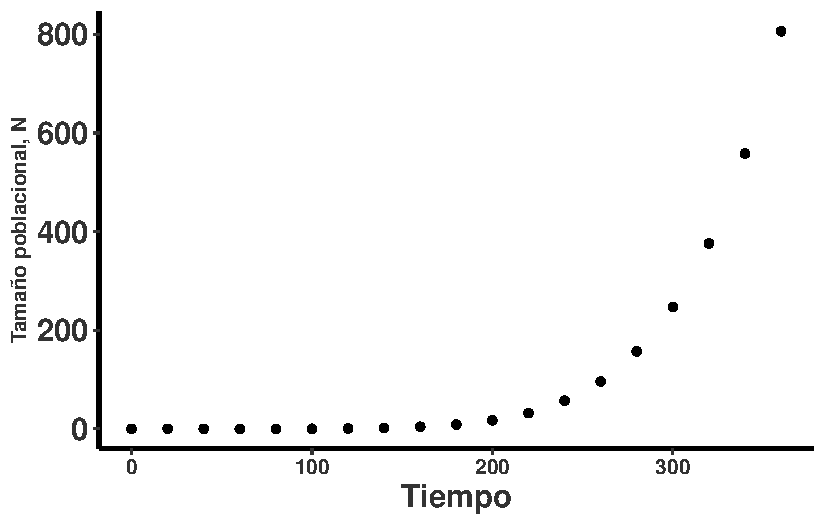
\includegraphics[keepaspectratio]{102-Intro_files/figure-pdf/Pop-fig_1-1.pdf}}

}

\caption{Cambio poblacional en tiempo}

\end{figure}%

\section{Un recuento histórico breve de la ecología de
poblaciones}\label{un-recuento-histuxf3rico-breve-de-la-ecologuxeda-de-poblaciones}

Los primeros estudios poblacionales se enfocaron en contar cuántos
individuos de varias especies había en un sitio y en evaluar el impacto
de diferentes tipos de efectos antropogénicos o de especies invasoras
(Crawley, 1990). Crawley (Crawley, 1990) indica que los primeros
estudios publicados sobre el conteo de individuos en plantas fueron
realizados por Carr (1848) y Burdon (1856), ambos presidentes de la
Tyneside Natural History Society en Inglaterra. En la publicación de
Burdon se menciona la presencia de individuos de \emph{Cypripedium
calceolus} en Castle Eden Dene, en el condado de Durham, hasta la
pérdida completa de todos los individuos en 1850 (extraído de la
revisión de Michael J. Crawley (Crawley, 1990)). Sin embargo, al evaluar
la publicación original, desafortunadamente no se menciona la cantidad
exacta de individuos en el sitio (Baker \& Tate, 1867).

Otro estudio pionero sobre dinámica poblacional fue establecido por V.
M. Spalding en 1906 en el Carnegie Institute Desert Laboratory, con el
objetivo de contabilizar la cantidad de individuos del cactus saguaro
(\emph{Carnegiea gigantea}) y evaluar la reducción de esta especie en
relación con el aumento de la especie invasora \emph{Prosopis
glandulosa} y su correlación con el incremento de la ganadería en el
área.

En su revisión sobre la dinámica de poblaciones de plantas, Crawley
(Crawley, 1990) identifica siete componentes consistentes en la biología
vegetal:

\begin{itemize}
\item
  Plasticidad del tamaño: El tamaño de las plantas es una característica
  plástica, por lo que no constituye un buen indicador de la edad. Las
  correlaciones entre tamaño y edad varían entre especies (Gatsuk
  et~al., 1980; Roux \& McGeoch, 2004; Vanderklein et~al., 2007; Baden
  et~al., 2021).
\item
  Interacciones con vecinos: Debido a que las plantas son organismos
  sedentarios, la interacción con sus vecinos inmediatos es crucial. La
  densidad de individuos circundantes afecta su crecimiento,
  reproducción y supervivencia (Mitchell-Olds, 1987; Pantone, Baker \&
  Jordan, 1992; Postma et~al., 2021). En la revisión de Postma (Postma
  et~al., 2021), basada en 334 experimentos, se observa que al aumentar
  la densidad, el tamaño de las plantas disminuye junto con el número de
  tallos y ramas, aunque la altura permanece estable.
\item
  Cambios sucesionales: Las variaciones en la estructura poblacional a
  lo largo del tiempo son la norma, no la excepción (Young, Ewel \&
  Brown, 1987; Peña-Domene, Martı́nez-Garza \& Howe, 2013). Por ello, el
  reclutamiento y la supervivencia en una parcela específica pueden
  variar significativamente en tiempo y espacio, influenciados por
  factores bióticos y abióticos (Acácio et~al., 2007; Luzuriaga \&
  Escudero, 2008).
\item
  Reclutamiento impredecible: El reclutamiento puede ser infrecuente,
  impredecible y variable en el tiempo. Muchas especies forman bancos de
  semillas, lo que permite que el reclutamiento provenga de semillas
  almacenadas durante años (Saatkamp, Poschlod \& Venable, 2014; Fenner,
  2017; Tomowski et~al., 2023), incluso de diferentes cohortes.
\item
  Competencia asimétrica: La competencia intraespecífica (Weiner \&
  Thomas, 1986; Connolly \& Wayne, 1996; Weiner et~al., 2001) e
  interespecífica (Freckleton \& Watkinson, 2001) es común y
  generalmente asimétrica: las plantas grandes afectan a las pequeñas,
  pero rara vez ocurre lo contrario.
\item
  Mortalidad relacionada al tamaño: La mortalidad está fuertemente
  asociada al tamaño, siendo más frecuente en etapas o tamaños pequeños,
  tanto entre especies (Moles \& Westoby, 2006) como a nivel
  intraespecífico (Fricke, Tewksbury \& Rogers, 2019).
\item
  Oportunidades tras la muerte de individuos grandes: La muerte de
  plantas grandes y viejas, ya sea por accidentes, herbivoría o
  enfermedades, puede generar espacios que faciliten el reclutamiento
  (Wright et~al., 2003).
\end{itemize}

\section{El análisis de dinámica poblacional y su
uso}\label{el-anuxe1lisis-de-dinuxe1mica-poblacional-y-su-uso}

Determinar el tamaño poblacional futuro tiene múltiples aplicaciones,
que pueden agruparse en tres grandes categorías: 1) comprender las
interacciones ecológicas, 2) manejo y conservación, y 3) procesos
evolutivos. Los estudios enfocados en conservación se enmarcan dentro
del enfoque de viabilidad poblacional.

En este libro presentaremos una introducción a cada una de estas
vertientes. Nuestros ejemplos son ilustrativos y no constituyen una
profundización exhaustiva de cada tema. En la siguiente tabla se
muestran algunos usos específicos de la metodología de matriz de
proyección poblacional (MPP). La lista de aplicaciones proviene en parte
de las ideas de Morris y Doak (Morris \& Doak, 2002), con ampliaciones
posteriores.

\subsection{Tabla: El uso potencial de los diferentes acercamientos de
MPP}\label{tabla-el-uso-potencial-de-los-diferentes-acercamientos-de-mpp}

{\def\LTcaptype{none} % do not increment counter
\begin{longtable}[]{@{}
  >{\raggedright\arraybackslash}p{(\linewidth - 6\tabcolsep) * \real{0.2500}}
  >{\raggedright\arraybackslash}p{(\linewidth - 6\tabcolsep) * \real{0.2500}}
  >{\raggedright\arraybackslash}p{(\linewidth - 6\tabcolsep) * \real{0.2500}}
  >{\raggedleft\arraybackslash}p{(\linewidth - 6\tabcolsep) * \real{0.2500}}@{}}
\toprule\noalign{}
\begin{minipage}[b]{\linewidth}\raggedright
Categoría de Uso
\end{minipage} & \begin{minipage}[b]{\linewidth}\raggedright
Uso específico
\end{minipage} & \begin{minipage}[b]{\linewidth}\raggedright
Referencias generales
\end{minipage} & \begin{minipage}[b]{\linewidth}\raggedleft
Referencias con Orquídeas
\end{minipage} \\
\midrule\noalign{}
\endhead
\bottomrule\noalign{}
\endlastfoot
Manejo & Identificar las etapas o procesos demográficos claves &
(Crouse, Crowder \& Caswell, 1987) & (Shefferson et~al., 2003; Kéry \&
Gregg, 2004; Zotz \& Schmidt, 2006; Zhongjian et~al., 2008; Tremblay
et~al., 2009a,b) \\
& Determinar cuántos individuos en una población son necesarios para
reducir el riesgo de extinción & (Shaffer, 1981; Armbruster \& Lande,
1993; Traill, Bradshaw \& Brook, 2007; Flather et~al., 2011) & \\
& Determinar cuántos individuos se necesitan introducir en un sitio para
establecer una población viable & (Bustamante, 1996; Bell, Bowles \&
McEachern, 2003) & \\
& Determinar cuántos individuos se pueden extraer sin afectar
negativamente la viabilidad de una población & (Nantel, Gagnon \& Nault,
1996; Ticktin et~al., 2002; Ghimire et~al., 2008; Jansen et~al., 2018) &
(Ticktin et~al., 2020; Emeterio-Lara et~al., 2021) \\
& En especies invasoras, determinar cuántos individuos y en qué etapas
se deben remover para controlar la población & (Caplat, Coutts \&
Buckley, 2012; Arroyo-Cosultchi et~al., 2022) & \\
& Determinar cuántas poblaciones se necesitan para lograr la viabilidad
de una especie a nivel local o global & (Lindenmayer \& Possingham,
1996) & (Tremblay, Meléndez-Ackerman \& Kapan, 2006; Lind et~al., 2007;
Winkler, Hülber \& Hietz, 2009; Garcı́a González, Goñi \& Guzmán, 2010;
Kindlmann, Meléndez-Ackerman \& Tremblay, 2014) \\
Evaluación de riesgos & Evaluar el riesgo de extinción de una población
& (Gotelli \& Ellison, 2006) & (Nicolè, Brzosko \& Till-Bottraud, 2005;
Iriondo Alegria et~al., 2009; Hutchings, 2010; Thorpe et~al., 2011;
Raventós et~al., 2015; Hens et~al., 2017; Ackerman et~al., 2020; Berry
\& Cleavitt, 2021; Timsina et~al., 2021) \\
& Comparar el riesgo relativo entre dos o más poblaciones o especies &
(Earl, 2019) & (Schödelbauerová, Tremblay \& Kindlmann, 2010; Raventós
et~al., 2018; Crain, Tremblay \& Ferguson, 2019) \\
Interacciones ecológicas & Evaluar interacciones ecológicas abióticas y
bióticas para entender las variables importantes para la supervivencia
de una población & (Halpern \& Underwood, 2006; Mandle, Ticktin \&
Zuidema, 2015; Ehrlen et~al., 2016; Souza, Schmidt \& Conceicao, 2018) &
(Coates, Lunt \& Tremblay, 2006; Sletvold, Øien \& Moen, 2010; Sletvold
et~al., 2013; Ospina-Calderón et~al., 2023) \\
Procesos y patrones evolutivos & Identificar procesos, interacciones y
patrones evolutivos del ciclo de vida que impactan el crecimiento
poblacional & (Coste \& Pavard, 2020) & (Calvo, 1993; Jäkäläniemi
et~al., 2011; Shefferson et~al., 2012; Falcón, Ackerman \& Tremblay,
2017) \\
Metodología & Identificar la metodología adecuada según el tipo de
muestreo o historia de vida & (Van Groenendael et~al., 1994; Gerlach Jr
\& Rice, 2003; Rademaker, Leeuwen \& Smallegange, 2024; Jops, Dalling \&
O'Dwyer, 2025) & (Kéry \& Gregg, 2004; Gregg \& Kéry, 2006; Tremblay
et~al., 2009b, 2021; Shefferson, Warren \& Pulliam, 2014; Tremblay \&
McCarthy, 2014) \\
\end{longtable}
}

\section{Preguntas que aborda el análisis de dinámica
poblacional}\label{preguntas-que-aborda-el-anuxe1lisis-de-dinuxe1mica-poblacional}

\subsection{Identificar las etapas o procesos demográficos
claves}\label{identificar-las-etapas-o-procesos-demogruxe1ficos-claves}

Es fundamental reconocer cuáles son las etapas de vida más susceptibles
a cambios bióticos y abióticos, así como su impacto sobre la
persistencia de una población. Un ejemplo clásico en la literatura,
utilizando modelos matriciales por etapas (MPP), son los estudios sobre
la dinámica poblacional de la tortuga boba o cabezona (\emph{Caretta
caretta}) (Crouse, Crowder \& Caswell, 1987; Crowder et~al., 1994).
Crouse y Crowder demostraron que, aun salvando todos los huevos de la
depredación, esta estrategia tendría un impacto mínimo en el crecimiento
poblacional. El mayor efecto sobre la tasa de crecimiento se lograría
protegiendo a los adultos, específicamente reduciendo su mortalidad en
redes de pesca mediante modificaciones que permitan su escape sin
ahogarse. Estos trabajos fueron pioneros en mostrar que es posible
simular diferentes escenarios basados en la historia de vida del
organismo y evaluar su impacto. Esto no implica que no se deba proteger
los huevos, sino que el beneficio es menor comparado con la protección
de los adultos.

En estudios realizados en Cuba hace casi 20 años sobre tres especies
epífitas (\emph{Cattleyopsis cubensis}, \emph{Dendrophylax lindenii} y
\emph{Encyclia bocourtii}), se demostró que la protección de individuos
adultos es esencial para mantener el equilibrio poblacional. Esto se
debe al alto valor reproductivo de los individuos más grandes, que
poseen mayor capacidad para reemplazar a los individuos jóvenes, los
cuales presentan mayor probabilidad de morir (Raventós et~al., 2021).
Entre los principales riesgos para estas especies se encuentran la
incidencia de huracanes, la mortalidad de las especies que actúan como
forófitos y, en menor medida, la depredación.

\subsection{Determinar cuántos individuos en una población son
necesarios para reducir el riesgo de
extinción}\label{determinar-cuuxe1ntos-individuos-en-una-poblaciuxf3n-son-necesarios-para-reducir-el-riesgo-de-extinciuxf3n}

El efecto del tamaño poblacional sobre la biología y la probabilidad de
extinción en poblaciones naturales está bien documentado (Shaffer \&
Samson, 1985; Nunney \& Campbell, 1993; Harris et~al., 2022). Surge
entonces la pregunta: ¿cuál es la probabilidad de extinción de una
población considerando la cantidad de individuos en cada etapa del ciclo
de vida?

En general, se observa que a menor tamaño poblacional (N), mayor es el
riesgo de extinción. Sin embargo, esta correlación puede variar si
algunas etapas del ciclo de vida presentan reducciones significativas o
si la probabilidad de sobrevivir o avanzar a la siguiente etapa es muy
baja.

En el caso de las orquídeas, se sabe que una de las etapas más
vulnerables es la de semilla, ya que en condiciones naturales depende
del establecimiento de una interacción micorrícica específica. Por
ejemplo, ¿cuál es la probabilidad de que las semillas se depositen en un
sitio adecuado, encuentren su hongo específico, germinen y cuenten con
las condiciones ambientales necesarias para crecer hasta convertirse en
juveniles? Estas transiciones son extremadamente raras.

Por consiguiente, al evaluar la viabilidad de una nueva población de
orquídeas, no basta con considerar la cantidad de individuos presentes;
también es necesario estimar la probabilidad de que las semillas lleguen
a convertirse en adultos reproductores. Darwin (Darwin, 1877) estimó que
un fruto de \emph{Orchis maculata} produce aproximadamente 6,200
semillas, y una planta puede generar hasta 30 cápsulas, lo que equivale
a 186,300 semillas. En un acre, la suma de todas las plantas podría
producir más de 32,400,000,000 semillas. Sin duda, la probabilidad de
que una semilla germine y llegue a ser una planta adulta es
extremadamente baja; de lo contrario, estaríamos cubiertos de orquídeas
en apenas dos generaciones.

\subsection{Determinar cuántos individuos se necesita introducir en un
sitio para establecer una población
viable}\label{determinar-cuuxe1ntos-individuos-se-necesita-introducir-en-un-sitio-para-establecer-una-poblaciuxf3n-viable}

Determinar cuántos individuos se necesitan introducir en un sitio para
establecer una población viable es una pregunta clave en conservación.
Naturalmente, a mayor cantidad de individuos reintroducidos, mayor será
la probabilidad de éxito, asumiendo que el área seleccionada permite la
supervivencia, crecimiento y reproducción en todas las etapas del ciclo
de vida. Sin embargo, los recursos son limitados, por lo que la pregunta
debería enfocarse en cuál es el número mínimo de individuos necesario
para garantizar un porcentaje determinado de éxito en el establecimiento
de una nueva población.

En los últimos años, diversas organizaciones y científicos han
implementado programas de reintroducción de especies en sus hábitats
nativos, e incluso en áreas urbanas ({Bellis et~al.}, 2024; {D'Agostino
et~al.}, 2024).

En Corea, dos estudios ilustran la complejidad del proceso. En la isla
de Jeju, se translocó la orquídea \emph{Thrixspermum japonicum}, cuya
población original era de aproximadamente 50 individuos, de los cuales
solo uno produjo frutos. A partir de este individuo se propagaron
plántulas que fueron reintroducidas en el sitio. De los 216 individuos
translocados, el 73\% sobrevivió el primer año y el 63\% el segundo año;
entre el 16\% y el 35\% produjo frutos en los dos años siguientes (Kim,
Kang \& Kim, 2016). En otro estudio, en la isla de Bogildo, se
reintrodujeron más de 13,000 individuos de \emph{Dendrobium moniliforme}
propagados artificialmente. Los autores demostraron que la ubicación y
las condiciones del microhábitat son variables críticas: las áreas
abiertas con luz solar directa favorecieron un crecimiento más rápido
que las zonas sombreadas, y la especie de árbol huésped también influyó
significativamente (Kim, Kang \& Kim, 2016).

Desafortunadamente, ninguno de estos estudios aplicó métodos de análisis
de viabilidad poblacional (PVA) para determinar el tamaño mínimo de
reintroducción necesario para establecer poblaciones viables. Además, no
se consideraron factores como la probabilidad de germinación y el éxito
en alcanzar la etapa adulta. Un ejemplo de esta complejidad es el
trabajo de Zoe Fae Smith (Smith, 2006), quien evaluó la germinación in
situ de \emph{Diuris fragrantissima} y \emph{D. punctata} en Australia
utilizando 640 mallas según el método de (Rasmussen \& Whigham, 1993).
Ninguna semilla germinó en campo, lo que evidencia la necesidad de
estudios más detallados sobre viabilidad y estrategias de
reintroducción.

En otro estudio, Zettler y colaboradores (Zettler \& McInnis, 1993)
evaluaron la germinación de semillas de \emph{Goodyera pubescens} en un
sitio de reintroducción en el estado de Illinois, EE.UU. Los autores
encontraron que la germinación de las semillas fue muy baja y que la
presencia de hongos micorrícicos específicos era esencial para este
proceso. En consecuencia, la reintroducción de orquídeas en un sitio
debe considerar la presencia de hongos micorrícicos adecuados, así como
la cantidad de individuos que se deberían reintroducir para garantizar
la viabilidad de la población.

\subsection{Determinar el número de individuos que pueden ser extraídos
sin comprometer la viabilidad
poblacional}\label{determinar-el-nuxfamero-de-individuos-que-pueden-ser-extrauxeddos-sin-comprometer-la-viabilidad-poblacional}

La extracción de individuos, seudobulbos o flores desde su ambiente
natural responde principalmente a tres propósitos:

\begin{itemize}
\tightlist
\item
  Obtención de individuos para programas de conservación ex situ.
\item
  Utilización de un grupo de individuos para su propagación.
\item
  Extracción con fines comerciales sin objetivos de conservación (por
  ejemplo, uso medicinal, cultivo ornamental u otros usos).
\end{itemize}

Se suele asumir que la colecta de individuos de especies de orquídeas
desde sus hábitats naturales, tanto para conservación ex situ como para
propagación comercial, tiene un impacto mínimo y no afecta la
supervivencia poblacional a largo plazo. Sin embargo, este supuesto
requiere una evaluación crítica. La historia del fanatismo por la
recolección de orquídeas con fines comerciales está bien documentada
(Subedi et~al., 2013). Aunque se podría pensar que estas prácticas son
cosa del pasado, persisten casos de extracción ilegal por personas
inescrupulosas que no consideran el impacto sobre la población o la
especie ({Hinsley et~al.}, 2018).

\begin{tcolorbox}[enhanced jigsaw, arc=.35mm, bottomrule=.15mm, bottomtitle=1mm, breakable, colback=white, colbacktitle=quarto-callout-warning-color!10!white, colframe=quarto-callout-warning-color-frame, coltitle=black, left=2mm, leftrule=.75mm, opacityback=0, opacitybacktitle=0.6, rightrule=.15mm, title=\textcolor{quarto-callout-warning-color}{\faExclamationTriangle}\hspace{0.5em}{Advertencia}, titlerule=0mm, toprule=.15mm, toptitle=1mm]

\textbf{Cuidado con la ``extracción de bajo impacto''.} Es común suponer
que la recolección de un número reducido de individuos ---para
conservación \emph{ex situ}, propagación o uso comercial--- tiene un
impacto demográfico despreciable. Este supuesto requiere evaluación
crítica: el impacto depende del estadio extraído, de la elasticidad de
ese estadio sobre \(\lambda\), y de la frecuencia con que se repite la
extracción. Sin un análisis demográfico explícito, no se puede afirmar
que la extracción es sostenible.

\end{tcolorbox}

Por lo tanto, la pregunta central es: ¿cuántos individuos, y en qué
etapas del ciclo de vida, pueden ser extraídos sin afectar negativamente
el crecimiento poblacional? (Ticktin et~al., 2020). Responder esta
cuestión implica comprender la dinámica poblacional y aplicar modelos
que permitan estimar umbrales de extracción sostenible.

\subsection{En especies invasoras, determinar cuántos individuos y en
qué etapas se necesitan remover para controlar la
población}\label{en-especies-invasoras-determinar-cuuxe1ntos-individuos-y-en-quuxe9-etapas-se-necesitan-remover-para-controlar-la-poblaciuxf3n}

Actualmente, se reconoce ampliamente el impacto negativo que los
organismos invasores pueden ejercer sobre la flora y fauna nativas. Esto
plantea interrogantes fundamentales: ¿cuáles son las características que
confieren a una especie su potencial invasivo? y ¿qué programas de
manejo pueden implementarse para mitigar su impacto?

En términos generales, las especies invasoras se caracterizan por
presentar altas tasas de crecimiento y reproducción, elevada
supervivencia, baja mortalidad y gran capacidad de dispersión. Por
consiguiente, cualquier estrategia de manejo debe identificar las etapas
del ciclo de vida más vulnerables a la intervención. En la mayoría de
los casos, la etapa de semillas constituye el punto más susceptible para
la manipulación y control.

Los impactos más notorios de especies invasoras han sido documentados en
Australia, incluyendo la introducción del conejo (\emph{Oryctolagus
cuniculus}) (Alves et~al., 2022) y del cactus \emph{Opuntia} (Novoa
et~al., 2015), entre otros ejemplos ampliamente discutidos en cursos de
ecología de comunidades. No obstante, la problemática de las especies
invasoras continúa siendo un tema que requiere investigaciones y
evaluaciones más profundas.

Diversos estudios han empleado modelos de proyección poblacional (MPP)
para analizar la demografía de especies invasoras (Buckley, Briese \&
Rees, 2003; Koop \& Horvitz, 2005; McMahon \& Metcalf, 2008; Ramula
et~al., 2008; Li \& Ramula, 2015). Un caso particular evaluó el efecto
de una hormiga invasora y un insecto nativo sobre la dinámica
poblacional de una orquídea invasora (Falcón, Ackerman \& Tremblay,
2017).

\subsection{Evaluar el riesgo de una
población}\label{evaluar-el-riesgo-de-una-poblaciuxf3n}

La mayoría de los estudios que emplean modelos de proyección poblacional
(MPP, por sus siglas en inglés) se centran en evaluar el riesgo de
reducción poblacional o de extinción. Un ejemplo clásico es el trabajo
de Forsman (Forsman et~al., 1996), quien analizó 11 poblaciones del búho
moteado (spotted owl) y demostró que 10 de ellas estaban en declive,
mientras que la población de California se encontraba en riesgo de
extinción.

Los análisis basados en MPP como herramienta para estimar el riesgo de
extinción incluyen diferentes métricas, tales como la probabilidad de
extinción, la cuasiextinción y la probabilidad de cuasiextinción. Estas
estimaciones son fundamentales para especies cuyo manejo demográfico
busca reducir el riesgo de desaparición ({Crone et~al.}, 2011; Semmens
et~al., 2016). Sin embargo, aunque este enfoque es común en la
literatura de conservación, puede resultar problemático si no se
considera la confiabilidad de los parámetros estimados y la
incertidumbre asociada a los datos (Ludwig, 1999).

Un ejemplo del uso de MPP en orquídeas amenazadas es el caso de
\emph{Crepidium acuminatum}, una especie en peligro de extinción del
sudeste asiático, afectada por la extracción para uso medicinal (Timsina
et~al., 2021). Un estudio demográfico de seis años reveló que la tasa de
crecimiento poblacional fluctuó entre 0.80 y 1.05, sin diferencias
significativas entre años ni entre poblaciones. Otros ejemplos incluyen
el trabajo de (Borrero et~al., 2023), quienes estudiaron
\emph{Trichocentrum undulatum} y evaluaron el riesgo asociado a su
ubicación en la periferia de la distribución. En ambos casos, el
objetivo fue estimar el riesgo de extinción de las poblaciones
analizadas.

\subsection{Determinación del número de poblaciones necesarias para la
viabilidad de una especie a nivel local o
global}\label{determinaciuxf3n-del-nuxfamero-de-poblaciones-necesarias-para-la-viabilidad-de-una-especie-a-nivel-local-o-global}

La mayoría de las especies están divididas en múltiples poblaciones,
aunque el concepto de ``población'' puede variar según el contexto. Con
frecuencia, los autores no explicitan la definición utilizada y emplean
el término para referirse simplemente a una agrupación de individuos. La
definición práctica más común considera una población como un conjunto
de individuos suficientemente cercanos entre sí, lo que facilita la
recolección de datos. Sin embargo, este enfoque puede carecer de validez
ecológica o evolutiva.

En ecología, una población debería definirse como un grupo de individuos
que interactúan entre sí, o que al menos tienen cierta probabilidad de
hacerlo. Por ejemplo, si hablamos de una población de \emph{Catasetum},
los individuos deberían estar lo suficientemente próximos para que las
abejas polinizadoras (i.e., \emph{Euglossa} spp.) puedan transportar el
polen entre ellos. La distancia y el potencial de movimiento de estas
abejas varían considerablemente según la especie y la estructura del
paisaje (Tonhasca, Albuquerque \& Blackmer, 2003; Pokorny et~al., 2015;
Opedal et~al., 2017).

Otra definición, de carácter evolutivo, considera una población como el
conjunto de individuos entre los cuales ocurre flujo génico a lo largo
de una generación. El tiempo generacional depende de la longevidad de la
especie, que puede variar ampliamente. Por ejemplo, en las orquídeas
epífitas de ramitas (twig epiphytes), el ciclo generacional puede ser de
3 a 4 años, mientras que en \emph{Cypripedium calceolus}, una especie
terrestre de zonas templadas, los individuos adultos pueden vivir más de
50 años. Cabe destacar que la ``longevidad'' se define como la mediana
de la edad de los individuos en una población, excluyendo casos
extremos. El único estudio que ha evaluado la longevidad en orquídeas es
(Tremblay, 2000), limitado a especies del género \emph{Lepanthes}.

\begin{tcolorbox}[enhanced jigsaw, arc=.35mm, bottomrule=.15mm, bottomtitle=1mm, breakable, colback=white, colbacktitle=quarto-callout-tip-color!10!white, colframe=quarto-callout-tip-color-frame, coltitle=black, left=2mm, leftrule=.75mm, opacityback=0, opacitybacktitle=0.6, rightrule=.15mm, title=\textcolor{quarto-callout-tip-color}{\faLightbulb}\hspace{0.5em}{Recomendación}, titlerule=0mm, toprule=.15mm, toptitle=1mm]

\textbf{¿Qué es una población? Tres maneras de pensarlo.}

\begin{itemize}
\tightlist
\item
  \textbf{Operativa:} un grupo de individuos suficientemente cercanos
  para muestrearlos juntos. Útil en campo, pero sin justificación
  ecológica explícita.
\item
  \textbf{Ecológica:} un grupo de individuos que interactúan entre sí (o
  que pueden hacerlo) --- la distancia operativa depende de la movilidad
  del polinizador, dispersor, herbívoro, etc.
\item
  \textbf{Evolutiva:} un grupo entre el cual ocurre flujo génico durante
  una generación. La escala depende del tiempo generacional de la
  especie.
\end{itemize}

Estas definiciones a menudo no coinciden, y la elección afecta
directamente la interpretación de los resultados de un análisis de
dinámica poblacional.

\end{tcolorbox}

\subsection{Procesos y patrones evolutivos del ciclo de vida que
impactan el crecimiento
poblacional}\label{procesos-y-patrones-evolutivos-del-ciclo-de-vida-que-impactan-el-crecimiento-poblacional}

Un trabajo que aprovecha la MPP para evaluar procesos evolutivos es el
de Ricardo Calvo (Calvo, 1993), quien analizó la dinámica poblacional de
\emph{Tolumnia variegata} para determinar si la limitación de
polinizadores afecta su viabilidad. El estudio combinó experimentos de
polinización manual con modelos matriciales para estimar la tasa de
crecimiento poblacional bajo distintos niveles de polinización. Los
resultados mostraron que la fructificación natural es extremadamente
baja (\textless1 \%), pero aumenta significativamente con polinización
artificial, aunque con costos reproductivos en crecimiento y floración
futura. Las simulaciones sugieren que incluso una baja producción de
plántulas por fruto podría compensar estos costos, favoreciendo la
selección hacia mayor polinización. Sin embargo, la persistencia de baja
fructificación en orquídeas engañosas indica que la estrategia puede ser
estable si el reclutamiento de plántulas es limitado, resaltando la
importancia de considerar interacciones ecológicas y datos de
establecimiento para evaluar la viabilidad poblacional. Este caso nos
recuerda que la conservación y la evolución no dependen solo de la
presencia de individuos, sino de la compleja red de procesos que
sostienen la vida a largo plazo.

\begin{figure}[H]

{\centering \pandocbounded{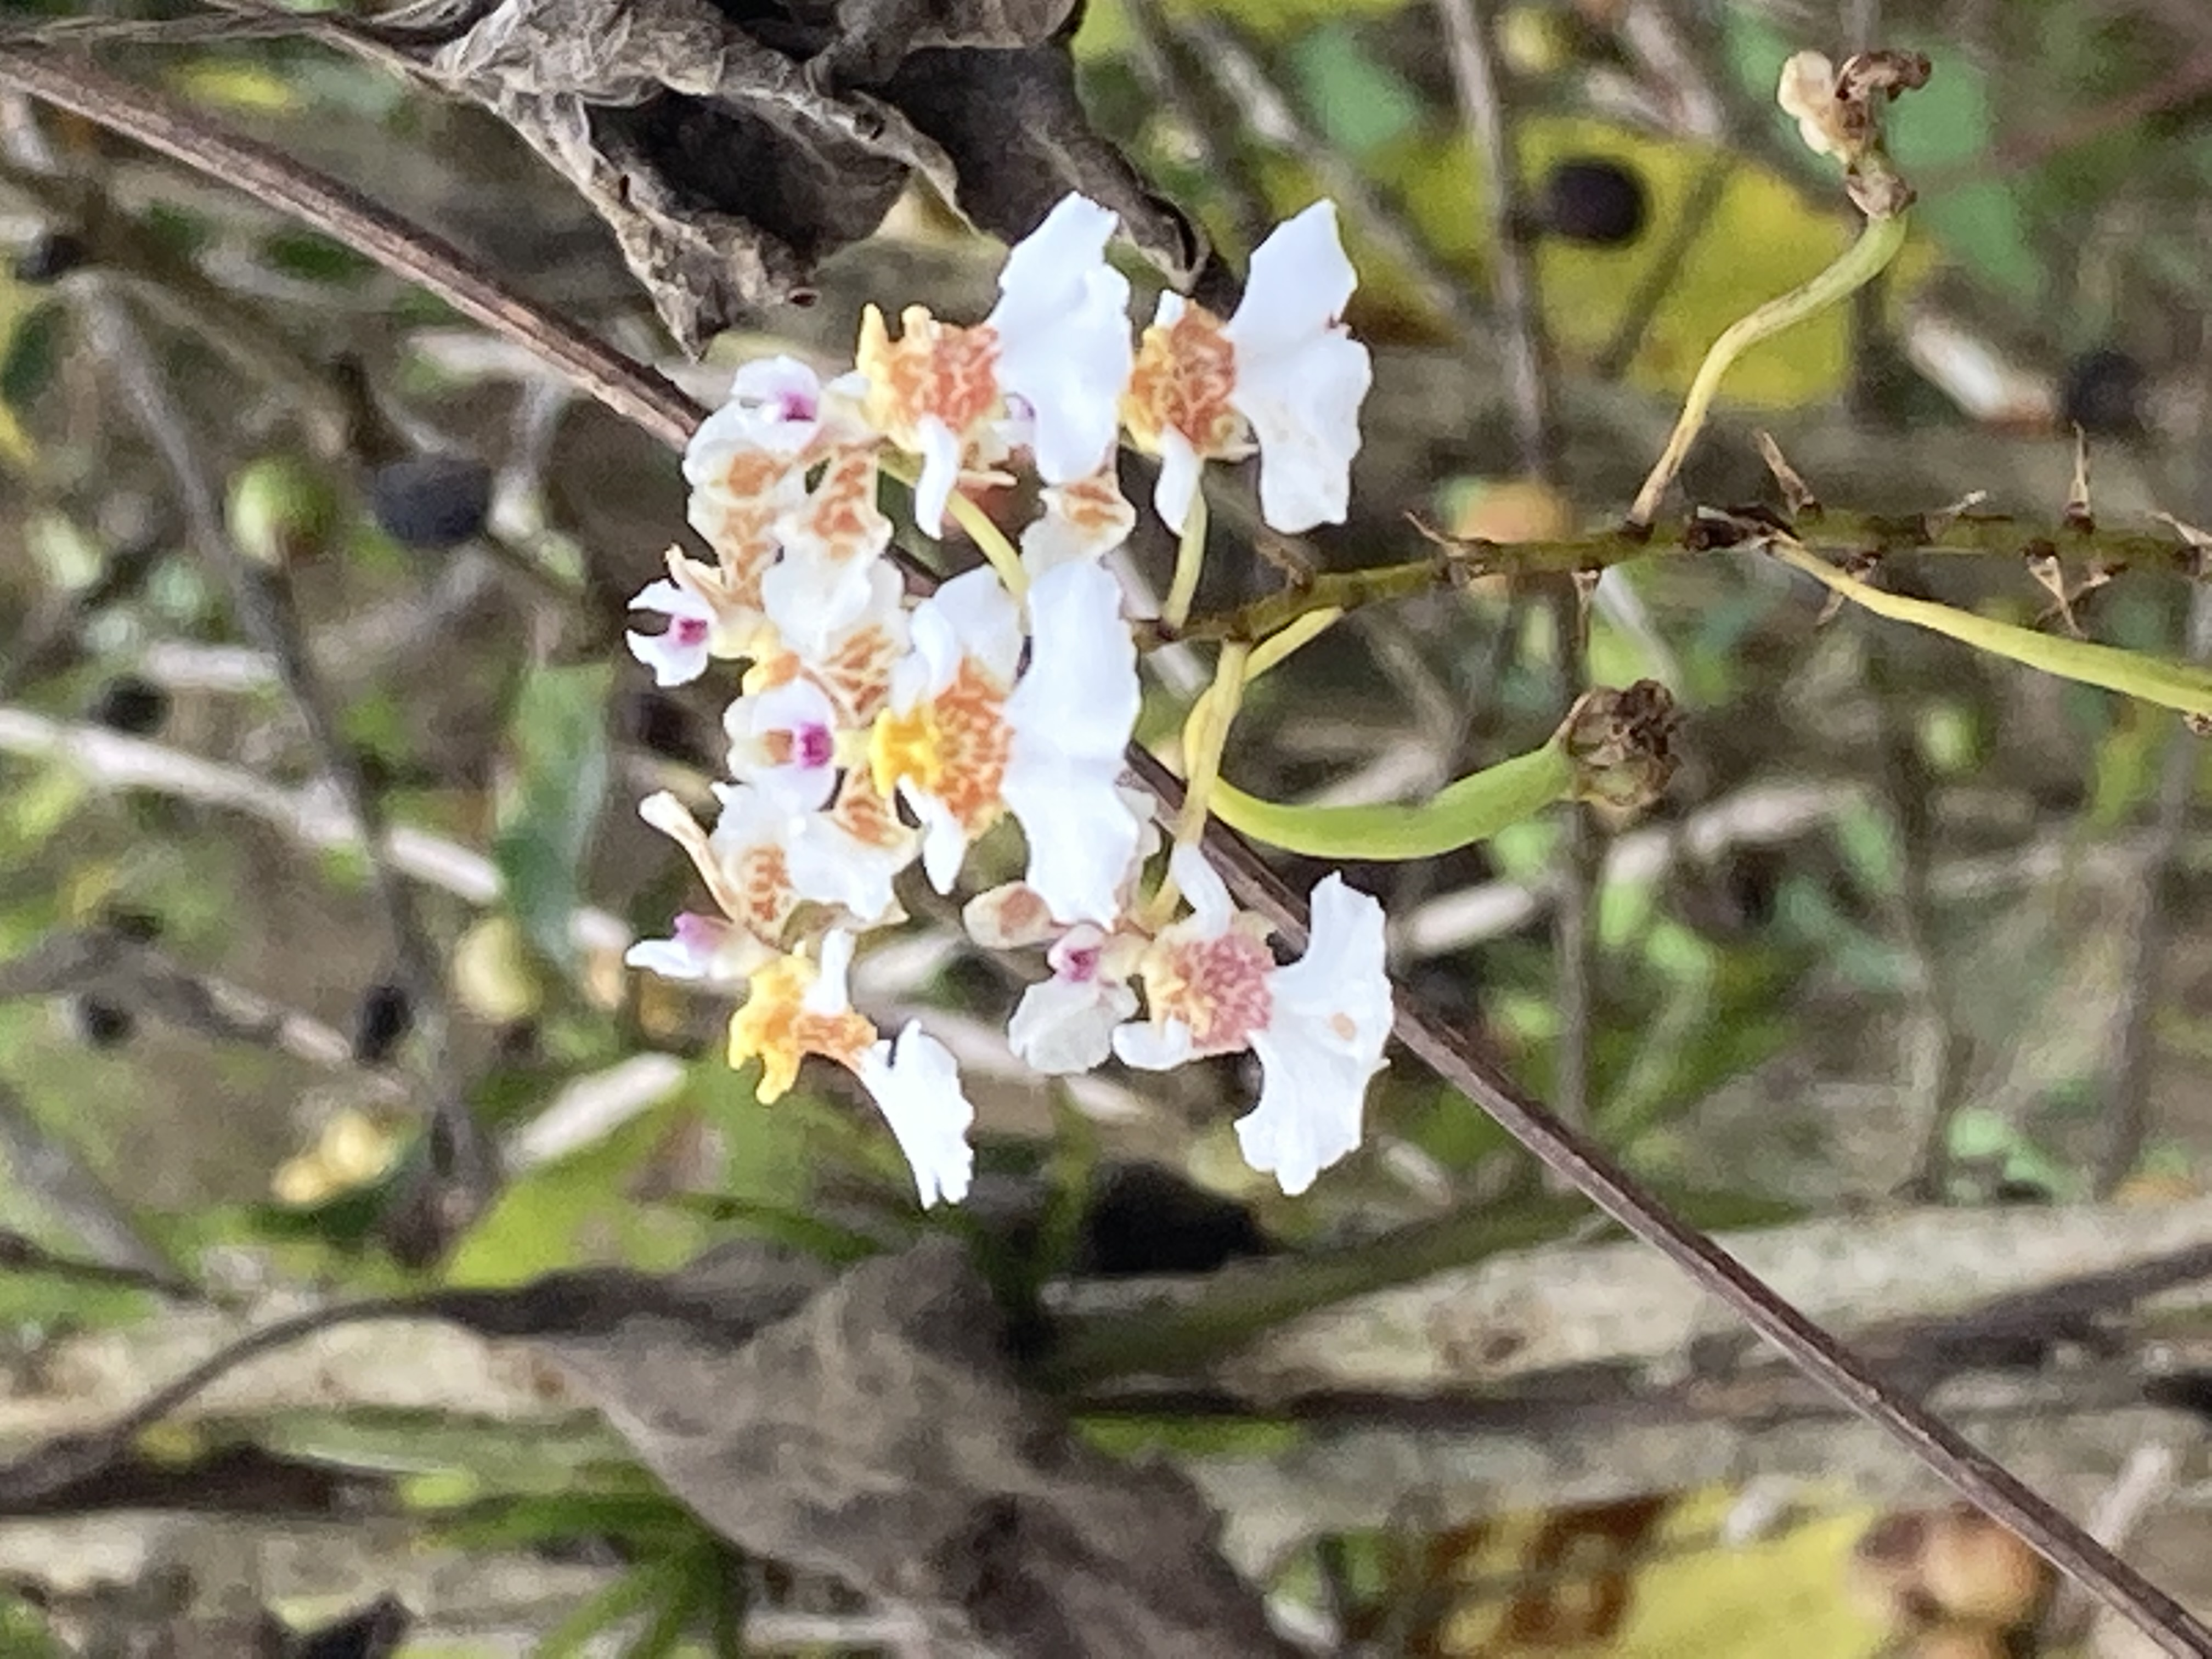
\includegraphics[keepaspectratio]{images/Tolumnia_variegata_Tremblay.jpeg}}

}

\caption{\emph{Tolumnia variegata}. Foto: Tremblay}

\end{figure}%

\begin{center}\rule{0.5\linewidth}{0.5pt}\end{center}

\section{Visualización de la dinámica
poblacional}\label{visualizaciuxf3n-de-la-dinuxe1mica-poblacional}

\begin{tcolorbox}[enhanced jigsaw, arc=.35mm, bottomrule=.15mm, bottomtitle=1mm, breakable, colback=white, colbacktitle=quarto-callout-important-color!10!white, colframe=quarto-callout-important-color-frame, coltitle=black, left=2mm, leftrule=.75mm, opacityback=0, opacitybacktitle=0.6, rightrule=.15mm, title=\textcolor{quarto-callout-important-color}{\faExclamation}\hspace{0.5em}{Importante}, titlerule=0mm, toprule=.15mm, toptitle=1mm]

\textbf{Un modelo es una caricatura útil, no una representación
completa.} Todo modelo demográfico es deliberadamente una
simplificación. Si se complica en exceso, los patrones no pueden
atribuirse a efectos identificables y el modelo pierde generalidad. El
criterio práctico es: un modelo debe ser \textbf{lo más simple posible,
pero no más simple} --- suficientemente parsimonioso para interpretarse,
pero suficientemente complejo para capturar los procesos esenciales.

\end{tcolorbox}

Representar el cambio poblacional mediante diagramas y sus posibles
causas permite integrar los diferentes componentes bióticos y abióticos
que influyen en la dinámica de una especie. Es importante aclarar que un
modelo es una simplificación ---una ``caricatura''--- y no incluye todos
los factores que afectan la población. El objetivo de un modelo es
reducir la complejidad biológica a los procesos más relevantes; si se
complica en exceso, los patrones y dinámicas no pueden atribuirse a
efectos proporcionalmente importantes. Además, un modelo demasiado
específico sería aplicable solo a una especie o población, limitando su
utilidad en otros sistemas.

En la figura se ilustran los factores principales que influyen en el
crecimiento poblacional y las variables más relevantes para evaluar el
riesgo de extinción. Todo análisis de dinámica poblacional parte del
tamaño de la población (N) o su densidad, ya que este parámetro impacta
directamente otros factores demográficos. En el diagrama, las líneas
entrecortadas con signos de interrogación indican relaciones con poca o
nula evidencia en orquídeas, mientras que las líneas continuas
representan factores respaldados por estudios.

Los efectos denso-dependientes pueden influir en el número de individuos
en el siguiente intervalo, así como las diferencias genéticas entre
ellos. Aunque esto se ha documentado en otros organismos, en orquídeas
los estudios son escasos y suelen asumir que las diferencias genéticas
tienen mayor impacto. Por el contrario, los efectos estocásticos
---tanto demográficos como ambientales--- son bien conocidos en
orquídeas y afectan los parámetros de crecimiento y su variación.
Finalmente, la variación temporal es el factor que más incide en el
riesgo de extinción: cuando esta variación es alta en poblaciones
pequeñas, la probabilidad de extinción aumenta significativamente. Por
ello, la variación en el tiempo debe considerarse en todos los estudios
de dinámica poblacional.

\begin{center}\rule{0.5\linewidth}{0.5pt}\end{center}

\begin{figure}[H]

{\centering 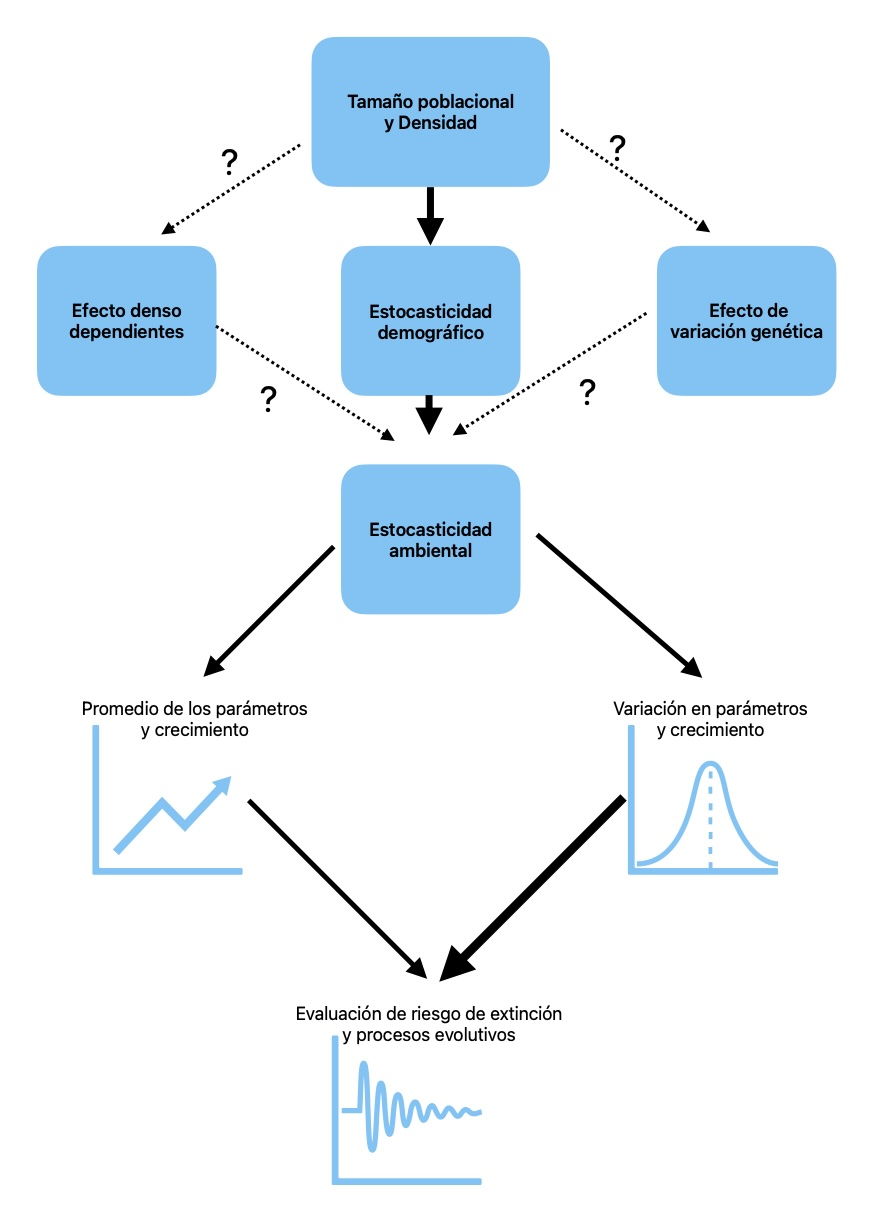
\includegraphics[width=0.5\linewidth,height=\textheight,keepaspectratio]{images/Demografia_de_una_poblacion.jpg}

}

\caption{Factores que influyen en la dinámica de una población}

\end{figure}%

\begin{center}\rule{0.5\linewidth}{0.5pt}\end{center}

\bookmarksetup{startatroot}

\chapter{El Ciclo de Vida}\label{Ciclo_Vida}

Raymond L. Tremblay

\subsubsection{Librerías de R requeridas para el siguiente
módulo}\label{libreruxedas-de-r-requeridas-para-el-siguiente-muxf3dulo-1}

\section{Introducción}\label{introducciuxf3n}

Todas las especies biológicas poseen una historia de vida que comienza
con el nacimiento y culmina con la muerte. En su hábitat natural, la
supervivencia de la mayoría de las plantas depende de la continuidad de
todas las etapas de desarrollo ---semilla, plántula, juvenil, adulto y
eventos reproductivos--- a lo largo del ciclo vital. Aunque estas etapas
suelen incluirse en los análisis, algunas pueden omitirse; por ejemplo,
la fase de semilla en especies que se reproducen vegetativamente
mediante clones (como plátanos, papas, piñas, vainillas y numerosas
plantas ornamentales y medicinales).

Desde la perspectiva de la conservación y la ecología, es fundamental
evaluar el ciclo de vida completo, identificar las características que
limitan la supervivencia y la reproducción en el hábitat natural, y
determinar cuáles etapas son más relevantes para el crecimiento
poblacional. La persistencia de una especie depende de procesos viables
que mantengan una población estable o en aumento. El método más adecuado
para evaluar esta persistencia consiste en analizar las etapas críticas
de la historia de vida y aplicar matrices de proyección poblacional para
estimar los cambios en el tiempo, identificando si la población crece,
disminuye o se mantiene estable.

Antes de iniciar cualquier estudio poblacional, se recomienda elaborar
un diagrama del ciclo de vida de la especie de interés. Este paso previo
a la recolección de datos permite visualizar el ciclo hipotético,
identificar etapas críticas, factores que influyen en el crecimiento y
supervivencia, y definir qué información debe obtenerse en campo. Los
diagramas son herramientas esenciales para comprender la biología del
organismo y anticipar los factores que afectan su desarrollo.

Un diagrama de ciclo de vida es una representación gráfica de los
estadios que atraviesa un organismo a lo largo de su existencia. En este
capítulo, se mostrará cómo crear diagramas de ciclo de vida en
\texttt{R} utilizando la librería \texttt{Rage}, enfatizando la
diferencia entre el modelo hipotético y los datos que pueden
recolectarse en campo.

\begin{tcolorbox}[enhanced jigsaw, arc=.35mm, bottomrule=.15mm, bottomtitle=1mm, breakable, colback=white, colbacktitle=quarto-callout-tip-color!10!white, colframe=quarto-callout-tip-color-frame, coltitle=black, left=2mm, leftrule=.75mm, opacityback=0, opacitybacktitle=0.6, rightrule=.15mm, title=\textcolor{quarto-callout-tip-color}{\faLightbulb}\hspace{0.5em}{Recomendación}, titlerule=0mm, toprule=.15mm, toptitle=1mm]

\textbf{Dibuja el ciclo de vida antes de salir al campo.} Elaborar un
diagrama hipotético del ciclo de vida ---con todas las etapas plausibles
y las transiciones entre ellas--- antes de iniciar el muestreo permite
identificar qué datos hacen falta, qué etapas son difíciles de observar
y qué transiciones son raras. Sin esa hoja de ruta, es fácil regresar
del campo con un conjunto de datos incompleto que no permite construir
una matriz biológicamente coherente.

\end{tcolorbox}

\begin{center}\rule{0.5\linewidth}{0.5pt}\end{center}

\section{Ejemplo de ciclos de vida
sencillo}\label{ejemplo-de-ciclos-de-vida-sencillo}

En este primer ejemplo se presenta un ciclo de vida simple con tres
estados: semillas, plántulas y adultos. Supongamos que se trata de una
planta que se reproduce sexualmente y cuyas semillas no forman un banco,
lo que implica que no hay latencia y germinan en el mismo año en que son
dispersadas. En este escenario, las semillas germinan y se convierten en
plántulas o mueren; las plántulas crecen y se transforman en adultos o
mueren; y los adultos se reproducen y finalmente mueren. Cada etapa dura
un año: el primero corresponde a la semilla, el segundo a la plántula y
el tercero al adulto, que contribuye con nuevas semillas. Por lo tanto,
el ciclo completo dura tres años. Este es un ejemplo hipotético, ya que
en la naturaleza los organismos rara vez presentan ciclos tan simples.

La matriz de transición para este ciclo es la siguiente: el 50 \% de las
semillas germinan y se convierten en plántulas, el 40 \% de las
plántulas alcanzan la etapa adulta y cada adulto produce en promedio 3.2
semillas. En el diagrama, las líneas verdes representan crecimiento y
las líneas amarillas representan reproducción.

\begin{Shaded}
\begin{Highlighting}[]
\CommentTok{\# 1) Build data/state as you already do}

\NormalTok{matA }\OtherTok{\textless{}{-}} \FunctionTok{rbind}\NormalTok{(}
  \FunctionTok{c}\NormalTok{(}\FloatTok{0.0}\NormalTok{, }\FloatTok{0.0}\NormalTok{, }\FloatTok{3.2}\NormalTok{),}
  \FunctionTok{c}\NormalTok{(}\FloatTok{0.5}\NormalTok{, }\FloatTok{0.0}\NormalTok{, }\FloatTok{0.0}\NormalTok{),}
  \FunctionTok{c}\NormalTok{(}\FloatTok{0.0}\NormalTok{, }\FloatTok{0.4}\NormalTok{, }\FloatTok{0.0}\NormalTok{)}
\NormalTok{)}
\NormalTok{etapas }\OtherTok{\textless{}{-}} \FunctionTok{c}\NormalTok{(}\StringTok{"semillas"}\NormalTok{, }\StringTok{"plantulas"}\NormalTok{, }\StringTok{"adultos"}\NormalTok{)}
\NormalTok{cols   }\OtherTok{\textless{}{-}} \FunctionTok{c}\NormalTok{(}\StringTok{"PaleGreen4"}\NormalTok{, }\StringTok{"PaleGreen4"}\NormalTok{, }\StringTok{"Goldenrod1"}\NormalTok{)}

\NormalTok{ne  }\OtherTok{\textless{}{-}} \FunctionTok{make\_nodes\_edges}\NormalTok{(etapas, matA, cols, }\AttributeTok{minlen\_scale =} \DecValTok{3}\NormalTok{, }\AttributeTok{digits =} \DecValTok{3}\NormalTok{, }\AttributeTok{fontsize =} \DecValTok{10}\NormalTok{)}
\NormalTok{dot }\OtherTok{\textless{}{-}} \FunctionTok{build\_dot}\NormalTok{(ne}\SpecialCharTok{$}\NormalTok{nodes, ne}\SpecialCharTok{$}\NormalTok{edges, }\AttributeTok{title =} \StringTok{"Especie hipotética"}\NormalTok{)}

\FunctionTok{render\_dual}\NormalTok{(dot, }\StringTok{"images/CV\_2.png"}\NormalTok{)}
\end{Highlighting}
\end{Shaded}

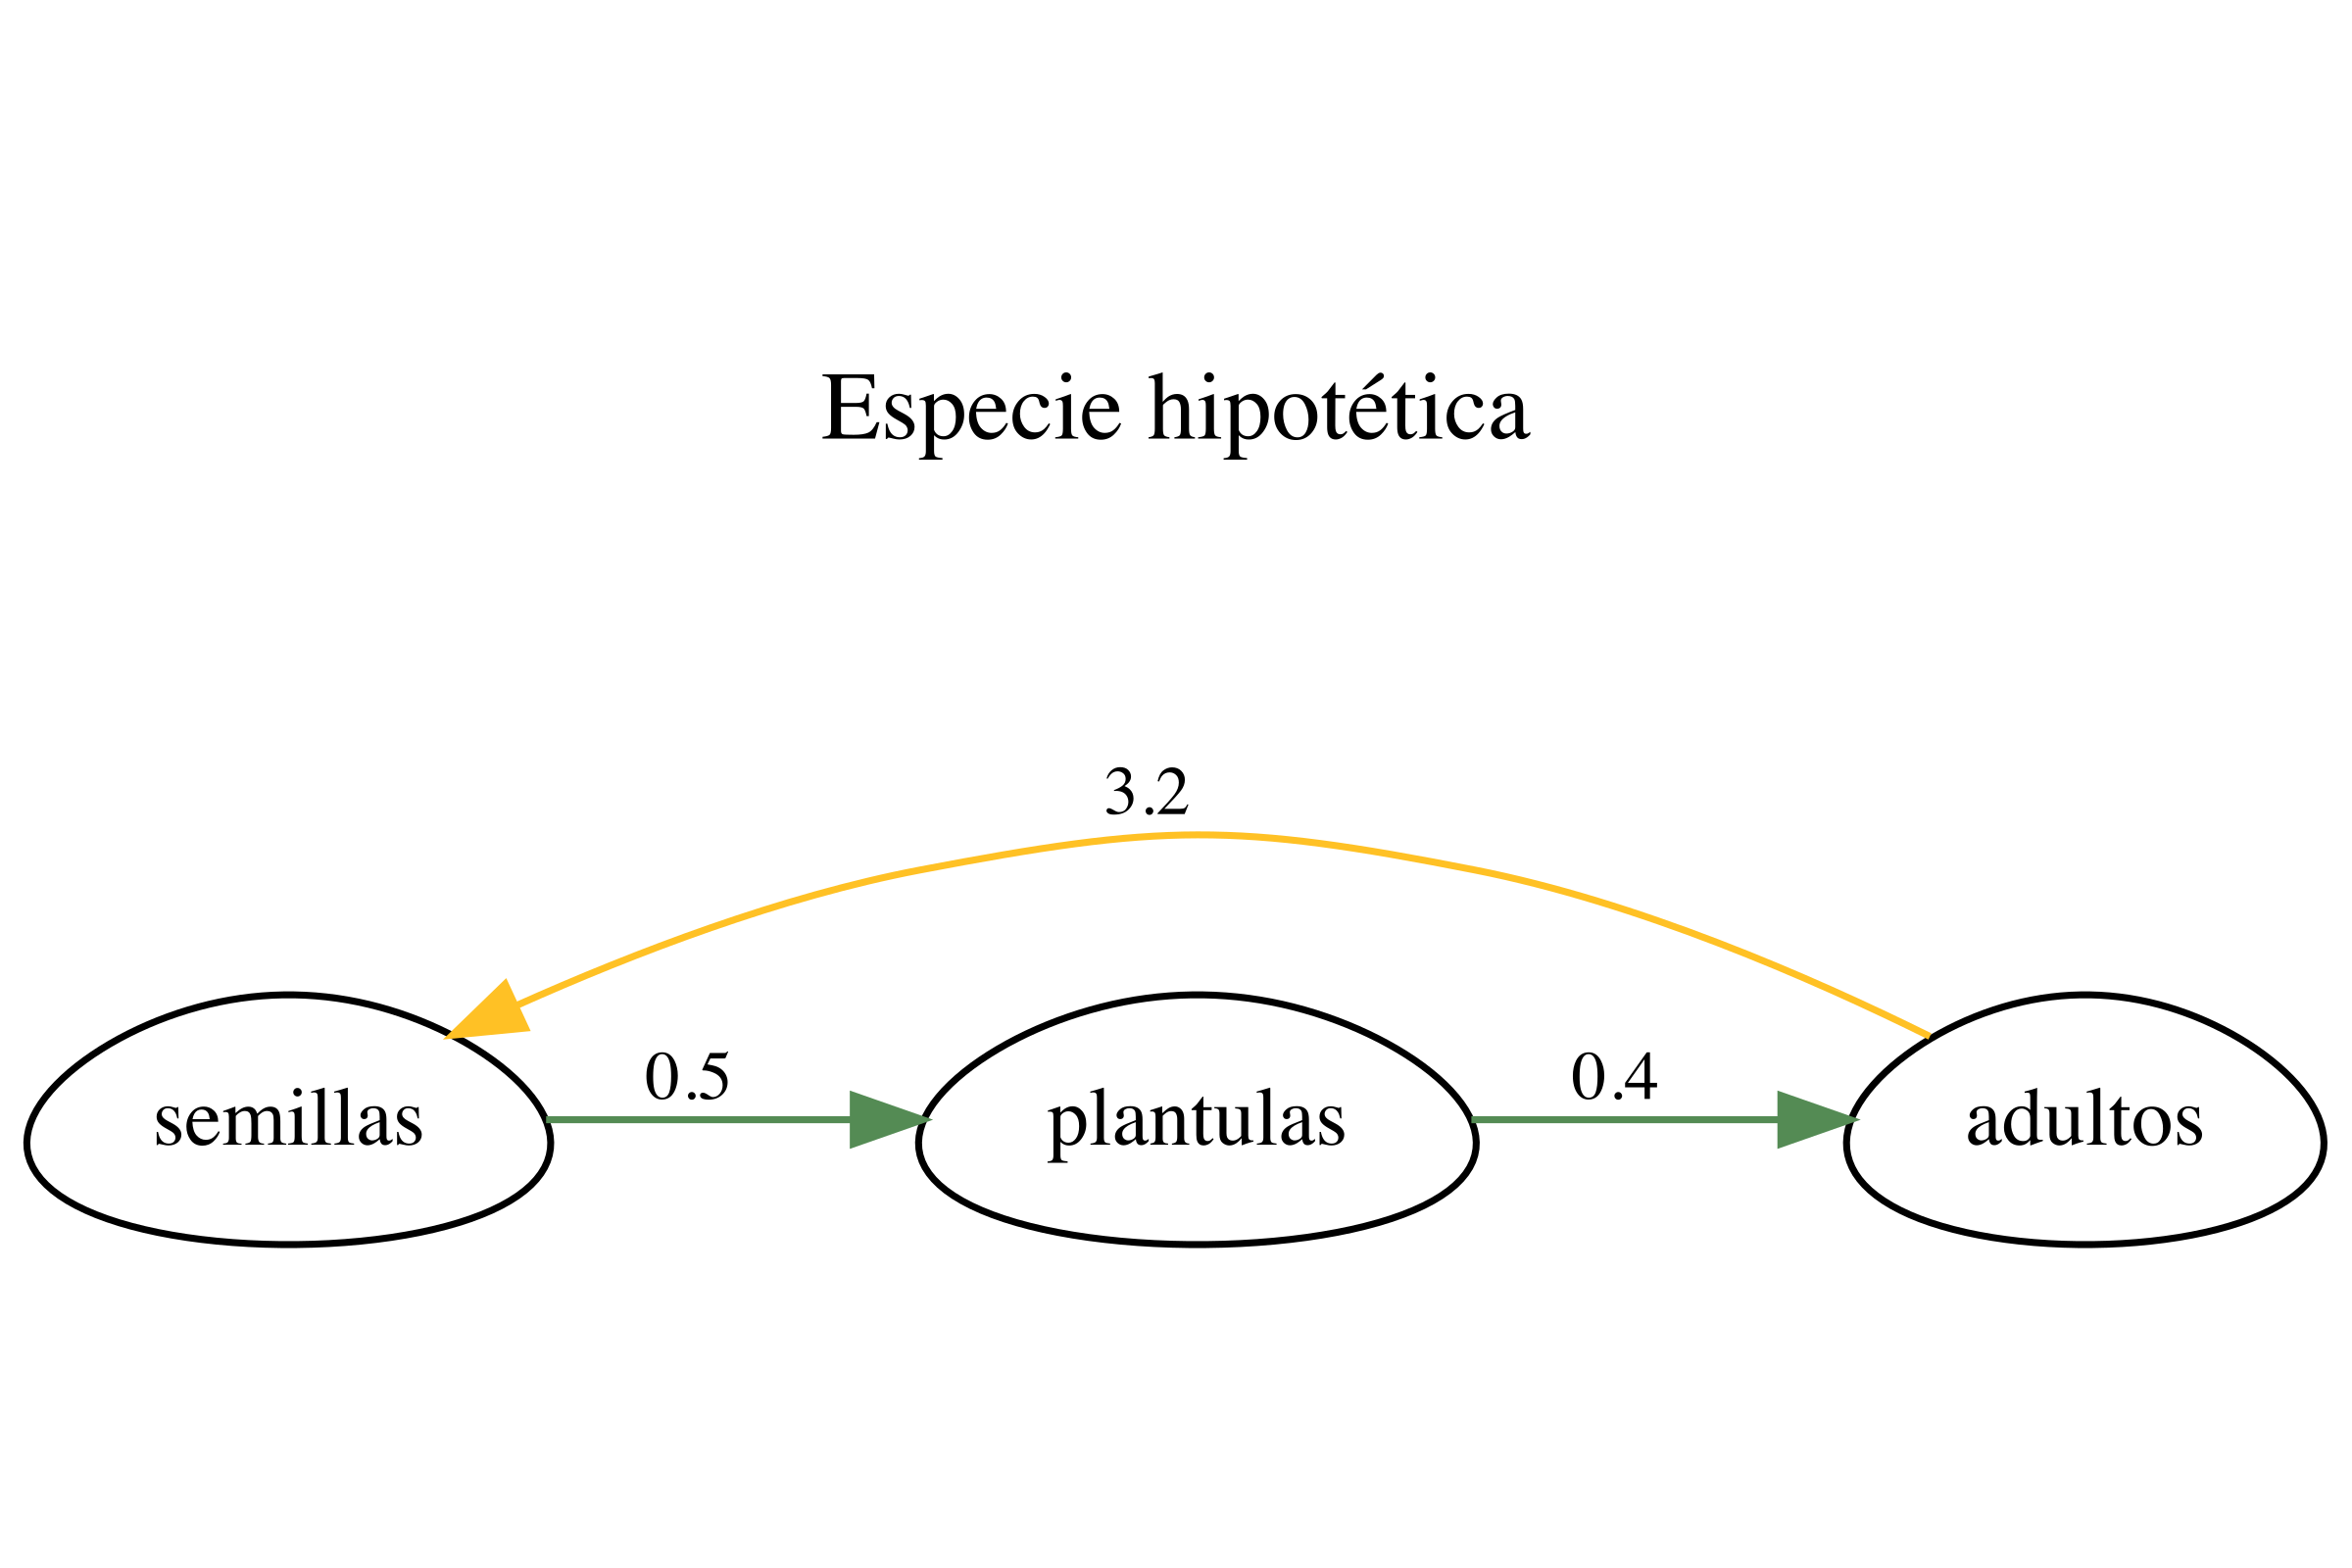
\includegraphics[width=8in,height=\textheight,keepaspectratio]{./images/CV_2.png}

\begin{center}\rule{0.5\linewidth}{0.5pt}\end{center}

\section{Ejemplo de una orquídea
hipotética}\label{ejemplo-de-una-orquuxeddea-hipotuxe9tica}

El ciclo de vida hipotético de una orquídea epífita se representa en el
gráfico mediante líneas verdes para indicar transición entre etapas,
líneas rojas para señalar permanencia y líneas amarillas para la
reproducción. El ciclo comienza con la germinación de la semilla sobre
la corteza de un árbol, seguida por las fases de plántula, juvenil y
adulto, etapa en la cual ocurre la floración y producción de semillas.
Exceptuando la fase de semilla, cada etapa puede prolongarse de un año a
otro, lo que evidencia un ciclo plurianual; esta característica se
refleja en la diagonal principal de la matriz de transición, cuyos
valores son mayores a cero cuando existe permanencia. Solo los
individuos adultos son capaces de reproducirse. Si el diagrama
correspondiera a datos empíricos, sería necesario contar con información
para todas las etapas (semilla, plántula, juvenil y adulto); sin
embargo, la revisión bibliográfica realizada no identificó estudios que
incluyan datos completos, debido principalmente a la dificultad de
localizar semillas y plántulas en condiciones naturales, dado su tamaño
extremadamente reducido (milimétrico) y la complejidad de seguir su
desarrollo a lo largo del tiempo.

\begin{Shaded}
\begin{Highlighting}[]
\NormalTok{matA\_ho }\OtherTok{\textless{}{-}} \FunctionTok{rbind}\NormalTok{(}
  \FunctionTok{c}\NormalTok{(}\FloatTok{0.0}\NormalTok{, }\FloatTok{0.0}\NormalTok{, }\FloatTok{0.0}\NormalTok{, }\FloatTok{3.2}\NormalTok{),}
  \FunctionTok{c}\NormalTok{(}\FloatTok{0.5}\NormalTok{, }\FloatTok{0.3}\NormalTok{, }\FloatTok{0.0}\NormalTok{, }\FloatTok{0.0}\NormalTok{),}
  \FunctionTok{c}\NormalTok{(}\FloatTok{0.0}\NormalTok{, }\FloatTok{0.4}\NormalTok{, }\FloatTok{0.20}\NormalTok{, }\FloatTok{0.0}\NormalTok{),}
  \FunctionTok{c}\NormalTok{(}\FloatTok{0.0}\NormalTok{, }\FloatTok{0.0}\NormalTok{, }\FloatTok{0.40}\NormalTok{, }\FloatTok{0.80}\NormalTok{)}
\NormalTok{)}
\NormalTok{etapas\_ho }\OtherTok{\textless{}{-}} \FunctionTok{c}\NormalTok{(}\StringTok{"semillas"}\NormalTok{, }\StringTok{"plantulas"}\NormalTok{, }\StringTok{"juvenil"}\NormalTok{, }\StringTok{"adultos"}\NormalTok{)}
\NormalTok{cols      }\OtherTok{\textless{}{-}} \FunctionTok{c}\NormalTok{(}\StringTok{"PaleGreen4"}\NormalTok{, }\StringTok{"red"}\NormalTok{, }\StringTok{"PaleGreen4"}\NormalTok{, }\StringTok{"red"}\NormalTok{, }\StringTok{"PaleGreen4"}\NormalTok{, }\StringTok{"Goldenrod1"}\NormalTok{, }\StringTok{"red"}\NormalTok{)}

\NormalTok{ne  }\OtherTok{\textless{}{-}} \FunctionTok{make\_nodes\_edges}\NormalTok{(etapas\_ho, matA\_ho, cols, }\AttributeTok{minlen\_scale =} \DecValTok{3}\NormalTok{, }\AttributeTok{digits =} \DecValTok{3}\NormalTok{, }\AttributeTok{fontsize =} \DecValTok{10}\NormalTok{)}
\NormalTok{dot }\OtherTok{\textless{}{-}} \FunctionTok{build\_dot}\NormalTok{(ne}\SpecialCharTok{$}\NormalTok{nodes, ne}\SpecialCharTok{$}\NormalTok{edges, }\AttributeTok{title =} \ConstantTok{NULL}\NormalTok{)}

\FunctionTok{render\_dual}\NormalTok{(dot, }\StringTok{"images/CV\_3.png"}\NormalTok{)}
\end{Highlighting}
\end{Shaded}

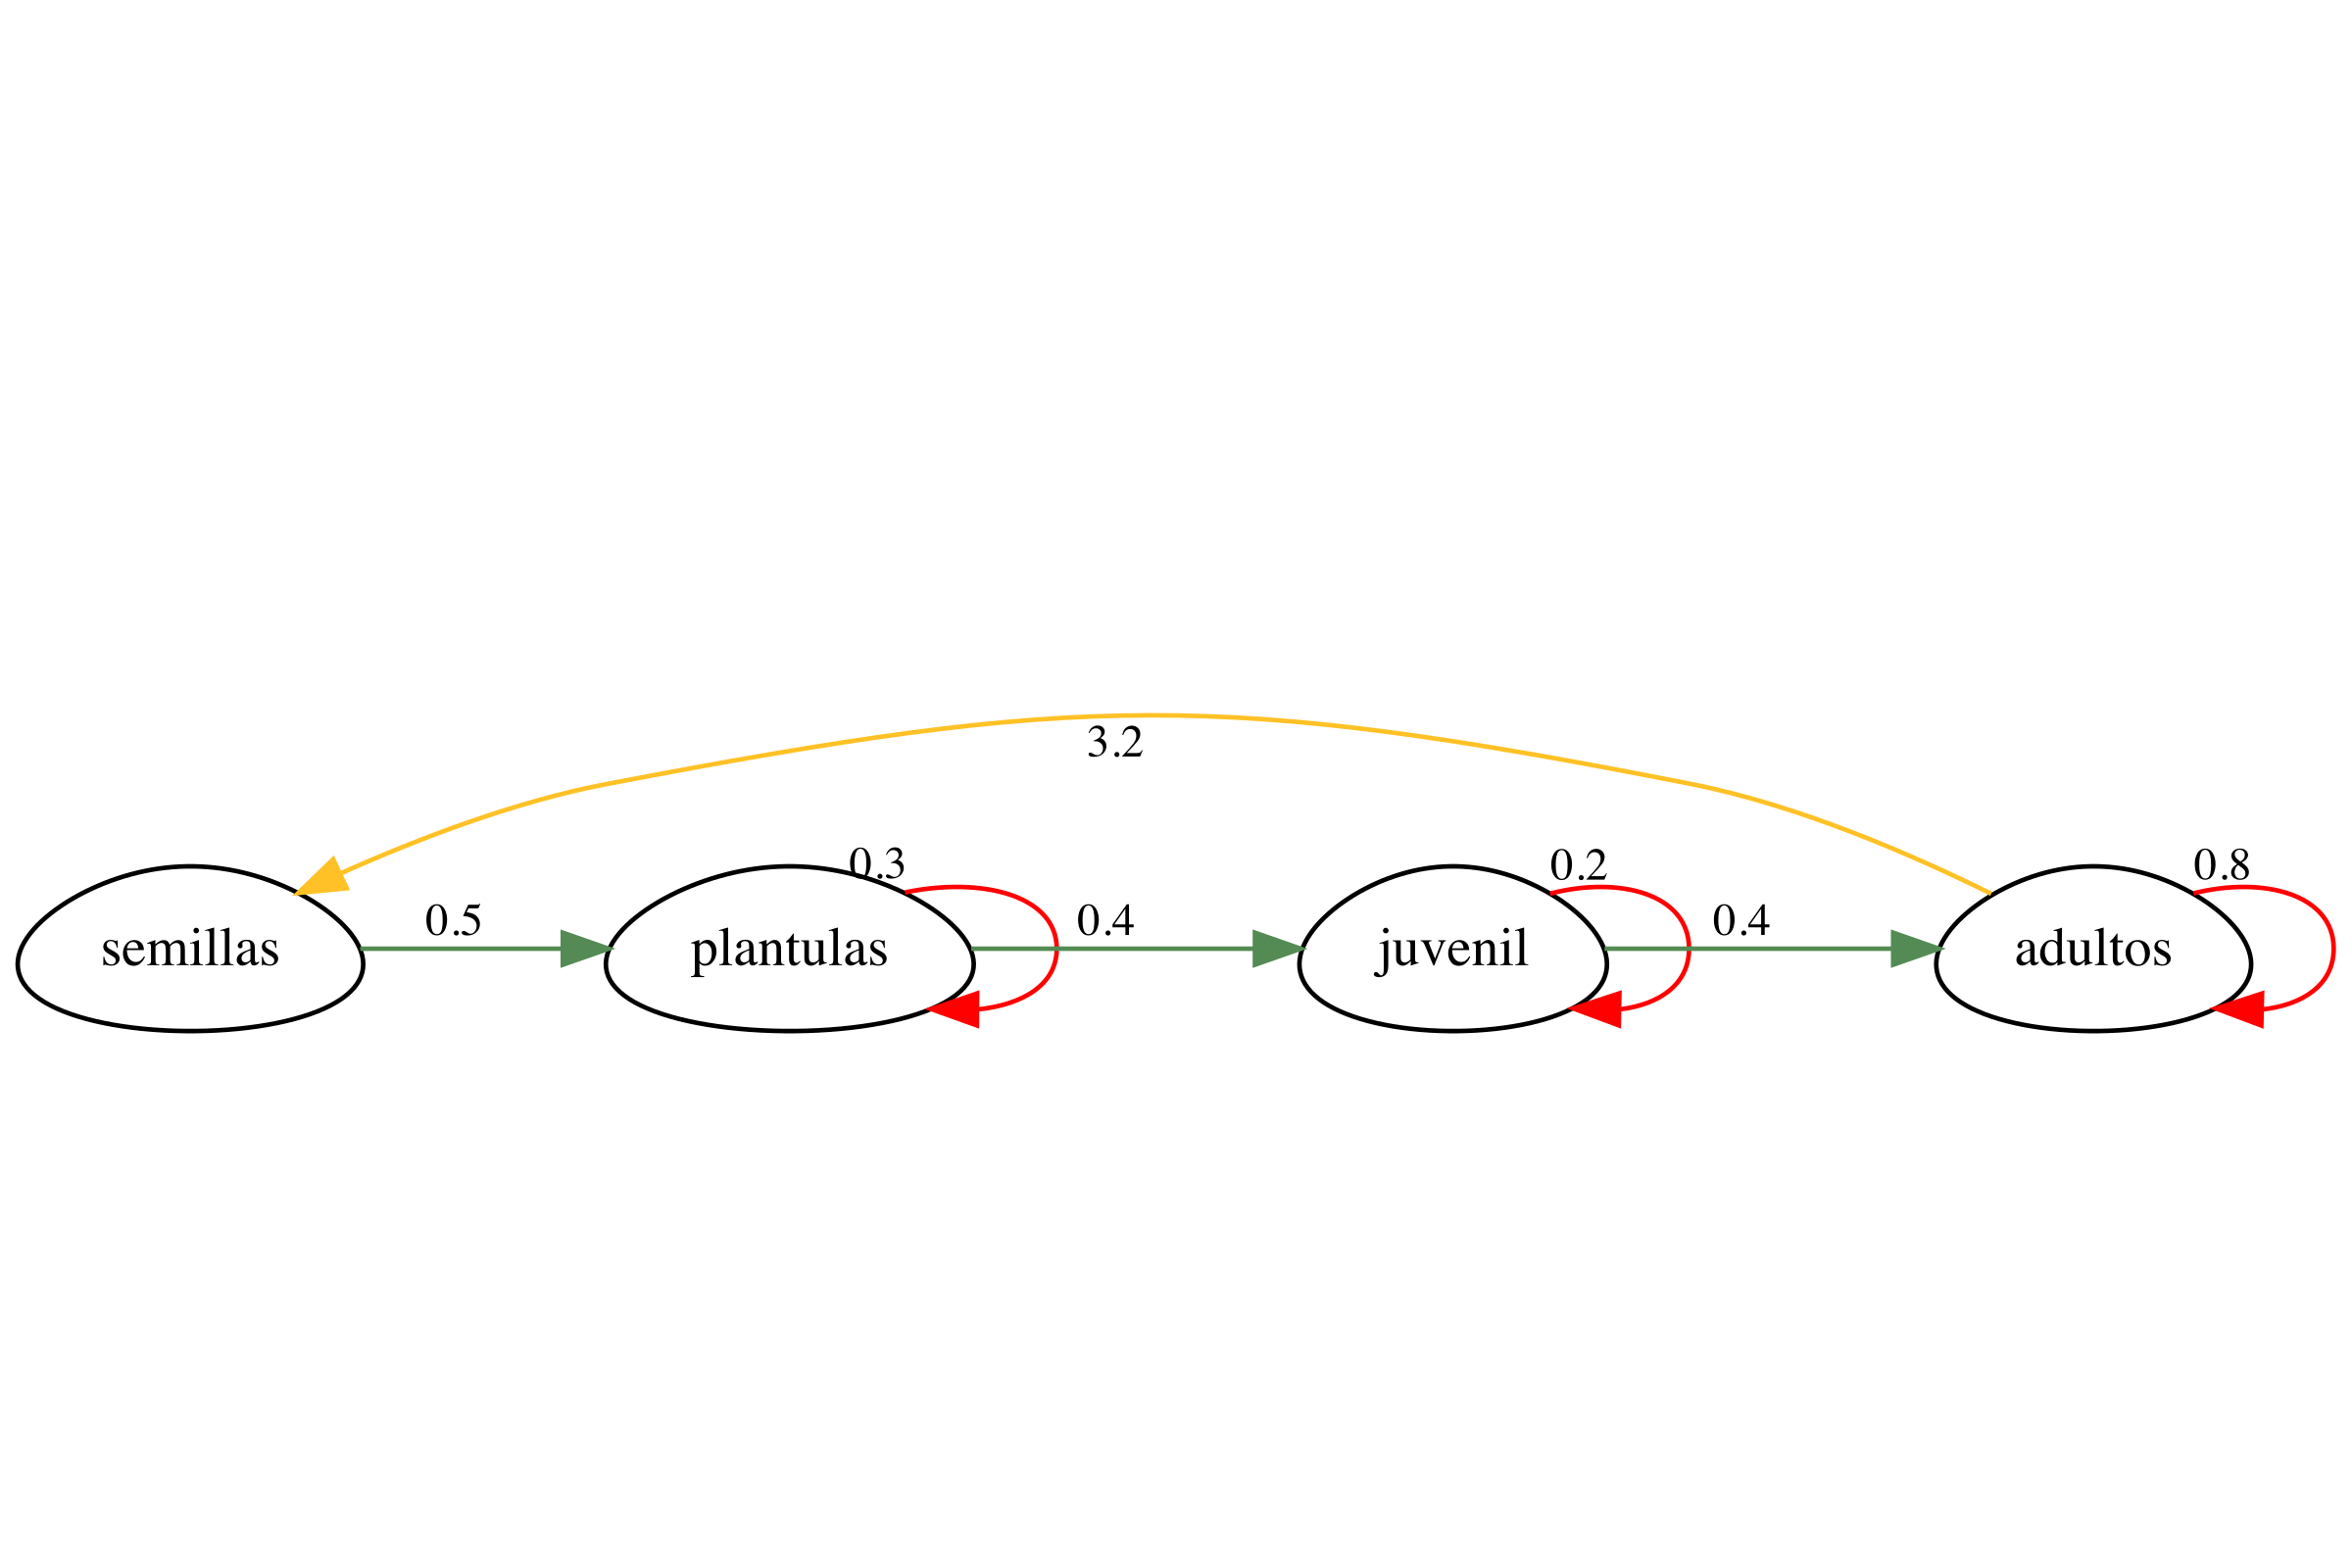
\includegraphics[width=8in,height=\textheight,keepaspectratio]{./images/CV_3.png}

\begin{center}\rule{0.5\linewidth}{0.5pt}\end{center}

\section{Ciclo de vida de orquídeas en la literatura
científica}\label{ciclo-de-vida-de-orquuxeddeas-en-la-literatura-cientuxedfica}

\begin{tcolorbox}[enhanced jigsaw, arc=.35mm, bottomrule=.15mm, bottomtitle=1mm, breakable, colback=white, colbacktitle=quarto-callout-note-color!10!white, colframe=quarto-callout-note-color-frame, coltitle=black, left=2mm, leftrule=.75mm, opacityback=0, opacitybacktitle=0.6, rightrule=.15mm, title=\textcolor{quarto-callout-note-color}{\faInfo}\hspace{0.5em}{Nota}, titlerule=0mm, toprule=.15mm, toptitle=1mm]

\textbf{Convención de colores en los diagramas de este capítulo.}

\begin{itemize}
\tightlist
\item
  \textbf{Verde:} crecimiento (transición a una etapa más avanzada)
\item
  \textbf{Rojo:} permanencia (mismo estadio en el siguiente intervalo)
\item
  \textbf{Amarillo:} reproducción (producción de semillas)
\item
  \textbf{Violeta:} regresión (transición a una etapa más temprana)
\item
  \textbf{Azul:} entrada o permanencia en latencia vegetativa
\end{itemize}

\end{tcolorbox}

A continuación se presentan diversos esquemas de ciclo de vida
utilizados en distintas publicaciones. Estos ejemplos evidencian la
ausencia de un modelo estandarizado, ya que cada investigador define un
ciclo particular en función de su comprensión del ciclo biológico de la
especie estudiada, la factibilidad de seguimiento de individuos a lo
largo del tiempo y los objetivos específicos de la investigación.

Los casos analizados incluyen tanto especies terrestres como epífitas, y
reflejan la diferencia entre los ciclos de vida hipotéticos y las
limitaciones impuestas por la recolección de datos en condiciones de
campo. Esta variabilidad pone de manifiesto la complejidad inherente al
estudio demográfico de orquídeas y la necesidad de adaptar los modelos a
las características ecológicas y metodológicas de cada estudio.

\subsection{Especies epífitas}\label{especies-epuxedfitas}

\subsubsection{\texorpdfstring{\emph{Laelia
speciosa}}{Laelia speciosa}}\label{laelia-speciosa}

La información presentada se basa en la tesina de Mariana
Hernández-Apolinar (Hernández-Apolinar, 1992), uno de los primeros
estudios sobre dinámica poblacional en orquídeas epífitas. El objetivo
principal de dicho trabajo fue evaluar el impacto de la recolección
sobre la dinámica poblacional de \emph{Laelia speciosa}.

El ciclo de vida propuesto se compone de cinco etapas, según lo
ilustrado en la figura 25a de la tesina:

\begin{itemize}
\tightlist
\item
  Semillas
\item
  Plántulas
\item
  3 etapas de tamaño de planta donde 2 de las etapas son adultos y
  pueden producir semillas
\end{itemize}

Es importante señalar que se realizó una estimación tanto de la cantidad
de semillas producidas como de la proporción que germina y se convierte
en plántula en el ciclo siguiente. Este enfoque permitió incorporar
procesos de transición y reproducción en el modelo, a pesar de las
limitaciones inherentes a la observación directa de semillas y plántulas
en condiciones naturales.

\begin{Shaded}
\begin{Highlighting}[]
\NormalTok{matA\_Ls }\OtherTok{\textless{}{-}} \FunctionTok{rbind}\NormalTok{(}
  \FunctionTok{c}\NormalTok{(}\FloatTok{0.0}\NormalTok{, }\FloatTok{0.0}\NormalTok{, }\FloatTok{0.00}\NormalTok{, }\DecValTok{52686}\NormalTok{, }\DecValTok{127324}\NormalTok{),}
  \FunctionTok{c}\NormalTok{(}\FloatTok{0.00022}\NormalTok{, }\FloatTok{0.0}\NormalTok{, }\FloatTok{0.00}\NormalTok{, }\FloatTok{0.0}\NormalTok{, }\FloatTok{0.0}\NormalTok{),}
  \FunctionTok{c}\NormalTok{(}\FloatTok{0.0}\NormalTok{, }\FloatTok{0.71}\NormalTok{, }\FloatTok{0.93}\NormalTok{, }\FloatTok{0.0}\NormalTok{, }\FloatTok{0.0}\NormalTok{),}
  \FunctionTok{c}\NormalTok{(}\FloatTok{0.0}\NormalTok{, }\FloatTok{0.0}\NormalTok{, }\FloatTok{0.07}\NormalTok{, }\FloatTok{0.76}\NormalTok{, }\FloatTok{0.0}\NormalTok{),}
  \FunctionTok{c}\NormalTok{(}\FloatTok{0.0}\NormalTok{, }\FloatTok{0.0}\NormalTok{, }\FloatTok{0.00}\NormalTok{, }\FloatTok{0.24}\NormalTok{, }\FloatTok{0.75}\NormalTok{)}
\NormalTok{)}
\NormalTok{etapas\_Ls }\OtherTok{\textless{}{-}} \FunctionTok{c}\NormalTok{(}\StringTok{"semillas"}\NormalTok{, }\StringTok{"plántulas"}\NormalTok{, }\StringTok{"adulto 1"}\NormalTok{, }\StringTok{"adulto 2"}\NormalTok{, }\StringTok{"adulto 3"}\NormalTok{)}
\NormalTok{cols      }\OtherTok{\textless{}{-}} \FunctionTok{c}\NormalTok{(}\StringTok{"PaleGreen4"}\NormalTok{,}\StringTok{"PaleGreen4"}\NormalTok{,}\StringTok{"red"}\NormalTok{,}\StringTok{"PaleGreen4"}\NormalTok{,}\StringTok{"Goldenrod1"}\NormalTok{,}\StringTok{"red"}\NormalTok{,}\StringTok{"PaleGreen4"}\NormalTok{,}
               \StringTok{"Goldenrod1"}\NormalTok{,}\StringTok{"red"}\NormalTok{)}

\NormalTok{ne  }\OtherTok{\textless{}{-}} \FunctionTok{make\_nodes\_edges}\NormalTok{(etapas\_Ls, matA\_Ls, cols, }\AttributeTok{minlen\_scale =} \DecValTok{3}\NormalTok{, }\AttributeTok{digits =} \DecValTok{5}\NormalTok{, }\AttributeTok{fontsize =} \DecValTok{10}\NormalTok{)}
\NormalTok{dot }\OtherTok{\textless{}{-}} \FunctionTok{build\_dot}\NormalTok{(ne}\SpecialCharTok{$}\NormalTok{nodes, ne}\SpecialCharTok{$}\NormalTok{edges, }\AttributeTok{title =} \ConstantTok{NULL}\NormalTok{)}

\FunctionTok{render\_dual}\NormalTok{(dot, }\StringTok{"images/CV\_5.png"}\NormalTok{)}
\end{Highlighting}
\end{Shaded}

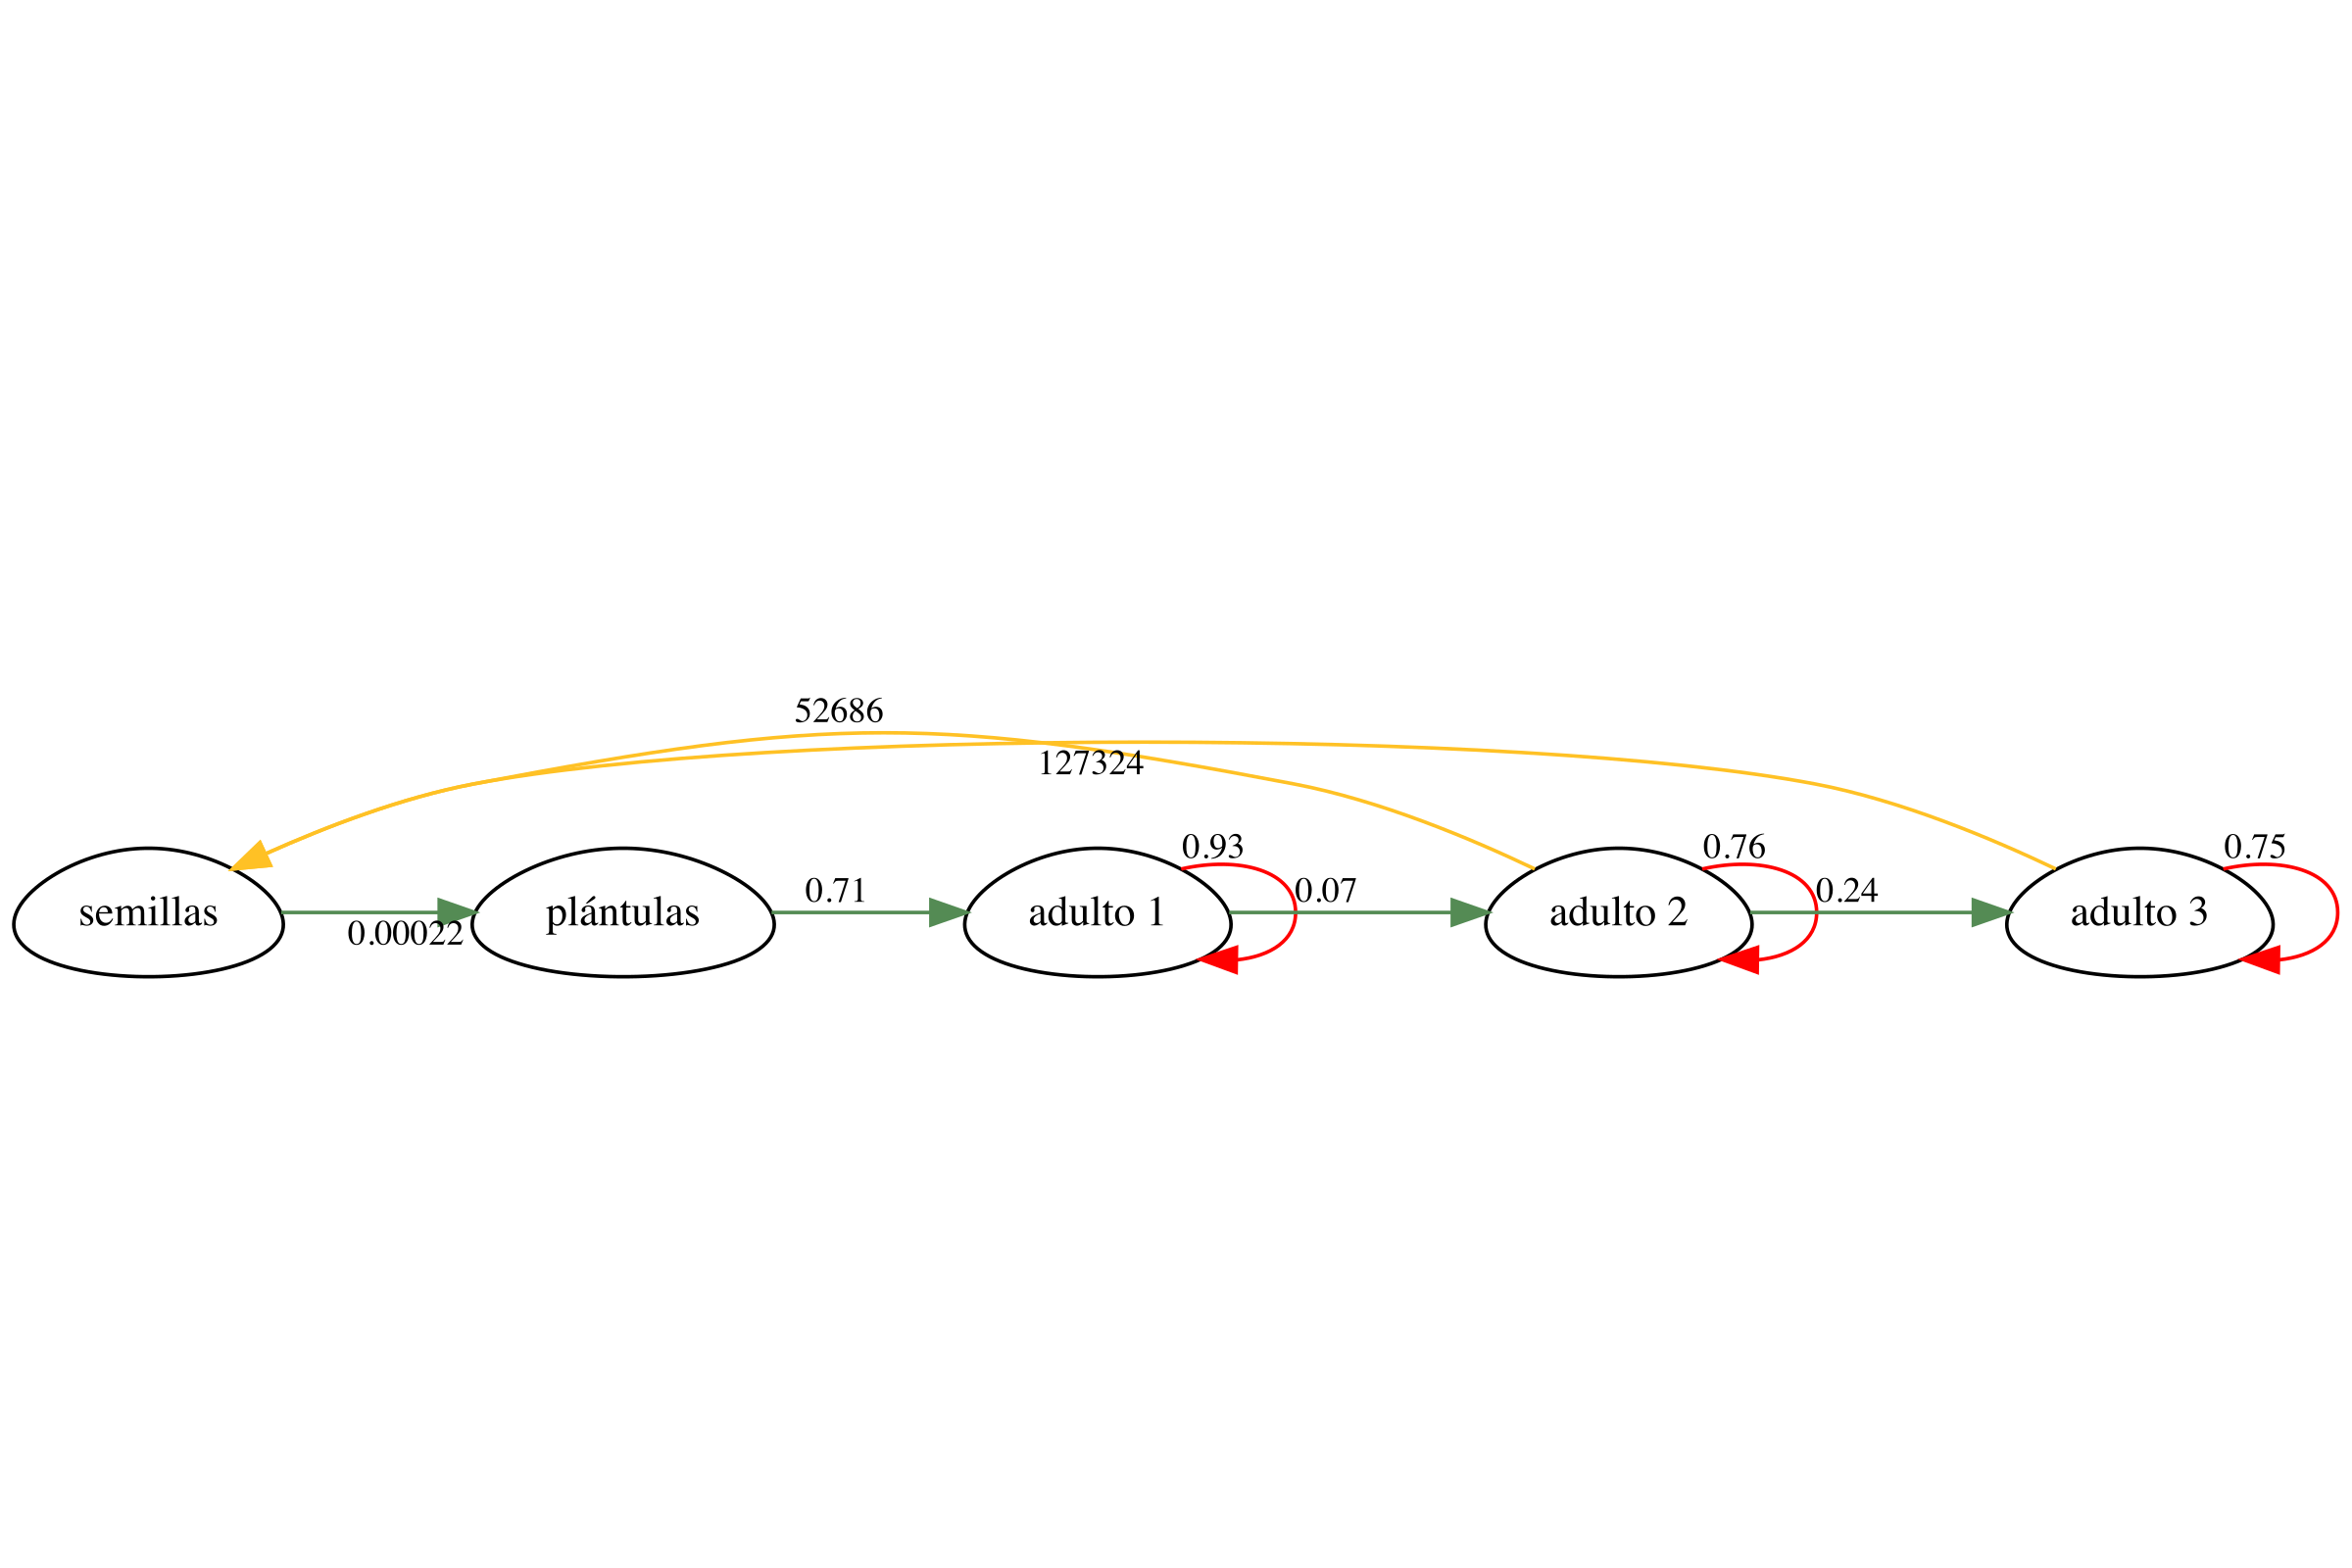
\includegraphics[width=8in,height=\textheight,keepaspectratio]{./images/CV_5.png}

\subsubsection{\texorpdfstring{\emph{Telipogon
helleri}}{Telipogon helleri}}\label{telipogon-helleri}

El estudio de (Raventós et~al., 2018) analizó la dinámica poblacional de
\emph{Telipogon helleri} considerando tres clases de tamaño: individuos
inmaduros, adultos reproductivos pequeños y adultos reproductivos
grandes. El ciclo de vida se representó mediante tres etapas, según lo
ilustrado en la figura 1 de la publicación. El objetivo principal fue
evaluar el efecto de las perturbaciones sobre el crecimiento
poblacional, utilizando un enfoque basado en análisis de dinámica
transitoria. Los autores identificaron tres tipos de transición en la
historia de vida de la especie:

\begin{itemize}
\tightlist
\item
  Transición a una etapa subsiguiente (indicada en verde)
\item
  Permanencia en la misma etapa (flechas rojas)
\item
  Regresión en tamaño (color violeta)
\item
  Reproducción (color amarillo)
\end{itemize}

Cabe destacar que los individuos adultos grandes presentan una mayor
contribución a la producción de semillas (0.5359) en comparación con los
adultos pequeños (0.1573), lo que subraya la importancia de la
estructura de tamaños en la dinámica poblacional.

\begin{Shaded}
\begin{Highlighting}[]
\NormalTok{matA\_Th }\OtherTok{\textless{}{-}} \FunctionTok{matrix}\NormalTok{(}\FunctionTok{c}\NormalTok{(}\FloatTok{0.1548}\NormalTok{, }\FloatTok{0.1573}\NormalTok{, }\FloatTok{0.5309}\NormalTok{,}
                    \FloatTok{0.2738}\NormalTok{, }\FloatTok{0.4425}\NormalTok{, }\FloatTok{0.1606}\NormalTok{,}
                    \FloatTok{0.0238}\NormalTok{, }\FloatTok{0.4060}\NormalTok{, }\FloatTok{0.7368}\NormalTok{),}
                  \AttributeTok{byrow =} \ConstantTok{TRUE}\NormalTok{, }\AttributeTok{ncol =} \DecValTok{3}\NormalTok{)}
\NormalTok{etapas\_Th }\OtherTok{\textless{}{-}} \FunctionTok{c}\NormalTok{(}\StringTok{"inmaduros"}\NormalTok{, }\StringTok{"reproductivo\_pequeños"}\NormalTok{, }\StringTok{"reproductivo\_grandes"}\NormalTok{)}
\NormalTok{cols      }\OtherTok{\textless{}{-}} \FunctionTok{c}\NormalTok{(}\StringTok{"red"}\NormalTok{,}\StringTok{"PaleGreen4"}\NormalTok{,}\StringTok{"PaleGreen4"}\NormalTok{,}\StringTok{"Goldenrod1"}\NormalTok{,}\StringTok{"red"}\NormalTok{,}\StringTok{"PaleGreen4"}\NormalTok{,}
               \StringTok{"Goldenrod1"}\NormalTok{,}\StringTok{"MediumOrchid4"}\NormalTok{,}\StringTok{"red"}\NormalTok{)}

\NormalTok{ne  }\OtherTok{\textless{}{-}} \FunctionTok{make\_nodes\_edges}\NormalTok{(etapas\_Th, matA\_Th, cols, }\AttributeTok{minlen\_scale =} \DecValTok{3}\NormalTok{, }\AttributeTok{digits =} \DecValTok{3}\NormalTok{, }\AttributeTok{fontsize =} \DecValTok{10}\NormalTok{)}
\NormalTok{dot }\OtherTok{\textless{}{-}} \FunctionTok{build\_dot}\NormalTok{(ne}\SpecialCharTok{$}\NormalTok{nodes, ne}\SpecialCharTok{$}\NormalTok{edges, }\AttributeTok{title =} \ConstantTok{NULL}\NormalTok{)}

\FunctionTok{render\_dual}\NormalTok{(dot, }\StringTok{"images/CV\_6Telipogon\_helleri.png"}\NormalTok{)}
\end{Highlighting}
\end{Shaded}

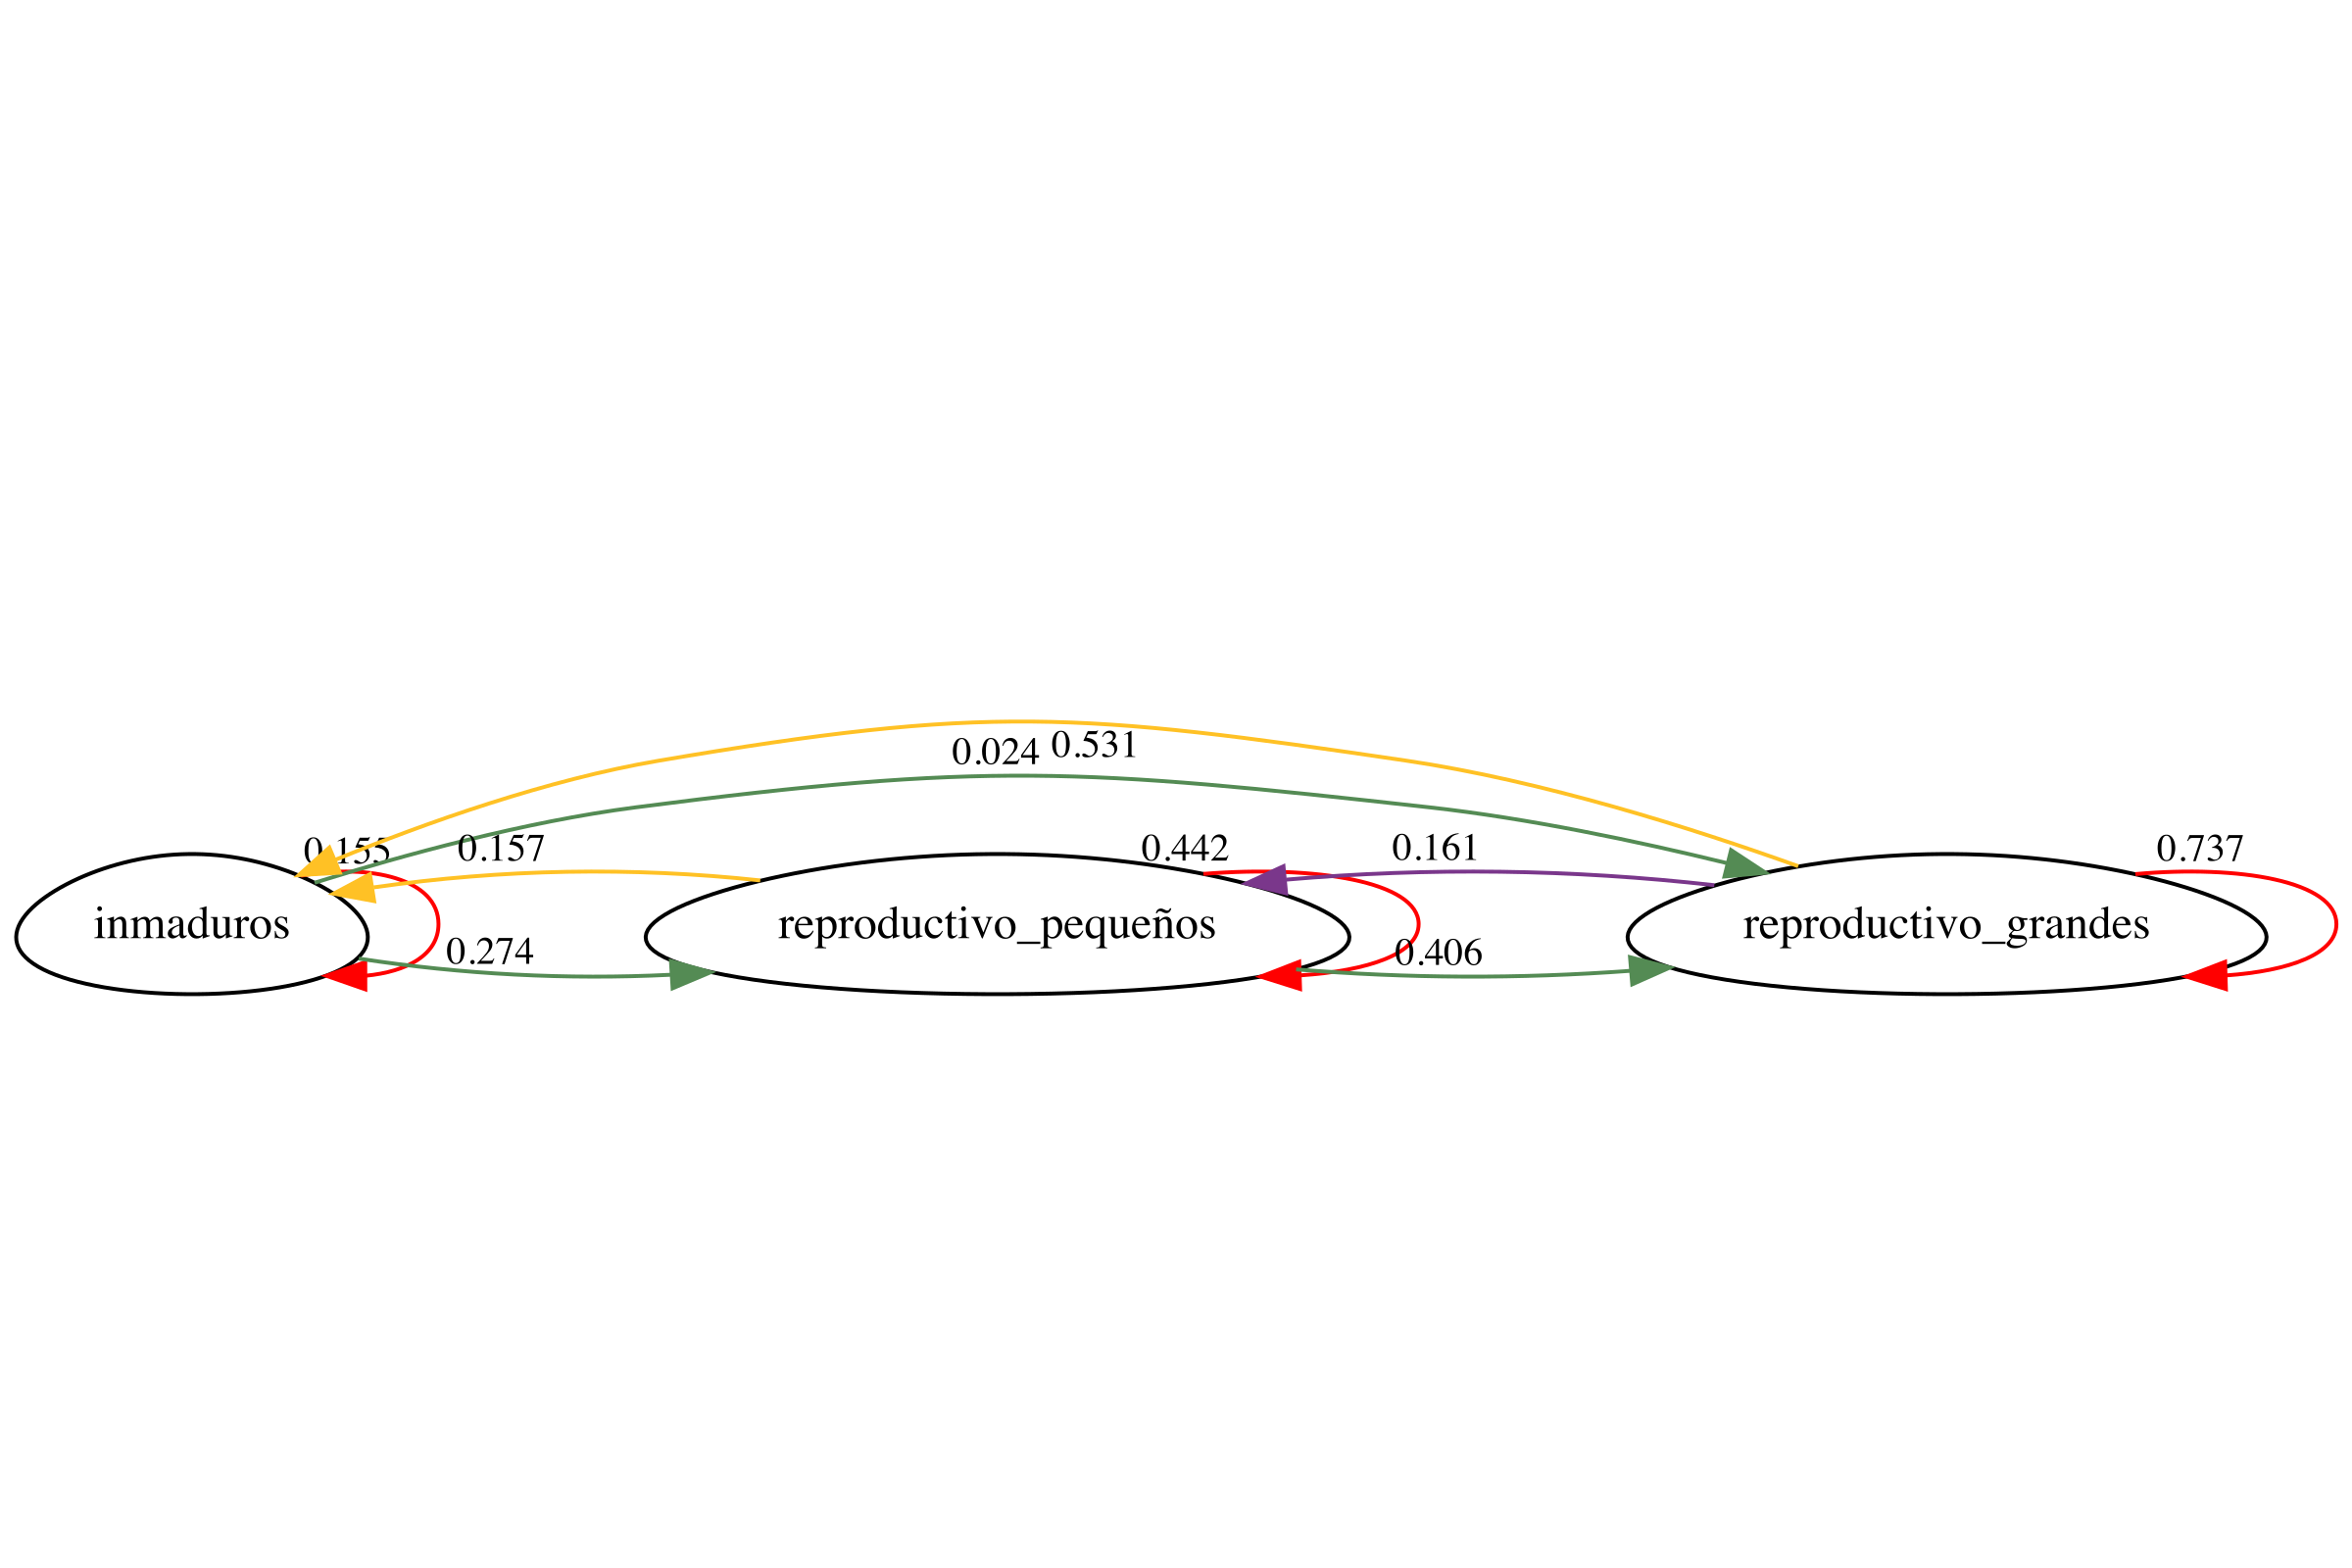
\includegraphics[width=8in,height=\textheight,keepaspectratio]{./images/CV_6Telipogon_helleri.png}

\subsection{Especies terrestres}\label{especies-terrestres}

\subsubsection{\texorpdfstring{\emph{Prasophyllum
correctum}}{Prasophyllum correctum}}\label{prasophyllum-correctum}

En el trabajo de Coates y colaboradores con \emph{Prasophyllum
correctum} se recolectaron datos de la etapa de plántula, juvenil,
adulto y latencia de los individuos (Coates, Lunt \& Tremblay, 2006). La
historia de vida de la especie está representada por 4 etapas. Los datos
provienen de la figura 4 de la publicación de (Coates, Lunt \& Tremblay,
2006), donde hay un periodo de 3 o más años entre los periodos de
régimen de fuegos. Una de la etapas distintivas de esta especie es la
latencia vegetativa, lo que significa que las plantas no emergen cada
año sus tubérculos (estructura de perennación) se mantienen vivos debajo
del suelo. Muchas especies de orquídeas terrestres tienen latencia en
las etapas de plántulas, juvenil y adultos.

En \emph{P. correctum}, al igual que en otras especies terrestres, es
difícil estimar su muerte debido a la presencia de latencia vegetativa.
Esto típicamente es un problema de muestreo y no de la biología de la
especie, ya que es muy difícil estimar la muerte de los individuos. La
ausencia de una planta marcada no significa que esté muerta, sino que
potencialmente está en su fase latente. Poder diferenciar un estado de
otro también es difícil, ya que no es ético modificar el hábitat para
determinar si la planta está viva o muerta, más aún si consideramos que
muchas de las especies terrestres están en peligro de extinción. Una
manera de dar solución a esta situación es hacer análisis para
determinar cuál es la probabilidad de que esté vivo un individuo con
latencia vegetativa de múltiples años. En este caso, se realizan
análisis usando un enfoque bayesiano (Tremblay et~al., 2009b) para
determinar cuál es la probabilidad de que un individuo con latencia de
múltiples años se encuentre vivo.

El tránsito a la fase de latencia vegetativa se indica en azul, en verde
el crecimiento, en amarillo la reproducción y en rojo la permanencia en
una misma etapa, incluyendo latente a latente.

\begin{tcolorbox}[enhanced jigsaw, arc=.35mm, bottomrule=.15mm, bottomtitle=1mm, breakable, colback=white, colbacktitle=quarto-callout-warning-color!10!white, colframe=quarto-callout-warning-color-frame, coltitle=black, left=2mm, leftrule=.75mm, opacityback=0, opacitybacktitle=0.6, rightrule=.15mm, title=\textcolor{quarto-callout-warning-color}{\faExclamationTriangle}\hspace{0.5em}{Advertencia}, titlerule=0mm, toprule=.15mm, toptitle=1mm]

\textbf{Ausencia no es muerte.} En orquídeas terrestres con latencia
vegetativa, la ausencia de una planta marcada en un censo \textbf{no}
implica que haya muerto: el tubérculo subterráneo puede estar vivo y
reaparecer años después. Asumir mortalidad cuando hay latencia subestima
la supervivencia y sesga las matrices de transición. Cuando se sospecha
latencia, conviene usar métodos bayesianos para estimar la probabilidad
de que un individuo ``ausente'' siga vivo (Tremblay et~al., 2009b).

\end{tcolorbox}

\begin{Shaded}
\begin{Highlighting}[]
\NormalTok{matA\_lat }\OtherTok{\textless{}{-}} \FunctionTok{rbind}\NormalTok{(}
  \FunctionTok{c}\NormalTok{(}\FloatTok{0.0}\NormalTok{, }\FloatTok{0.0}\NormalTok{, }\FloatTok{0.0125}\NormalTok{, }\FloatTok{0.0000}\NormalTok{),}
  \FunctionTok{c}\NormalTok{(}\FloatTok{0.0}\NormalTok{, }\FloatTok{0.2874}\NormalTok{, }\FloatTok{0.3750}\NormalTok{, }\FloatTok{0.1364}\NormalTok{),}
  \FunctionTok{c}\NormalTok{(}\FloatTok{0.0}\NormalTok{, }\FloatTok{0.0230}\NormalTok{, }\FloatTok{0.1500}\NormalTok{, }\FloatTok{0.0303}\NormalTok{),}
  \FunctionTok{c}\NormalTok{(}\FloatTok{1.0}\NormalTok{, }\FloatTok{0.6897}\NormalTok{, }\FloatTok{0.4750}\NormalTok{, }\FloatTok{0.7475}\NormalTok{)}
\NormalTok{)}
\NormalTok{etapas\_lat }\OtherTok{\textless{}{-}} \FunctionTok{c}\NormalTok{(}\StringTok{"plántulas"}\NormalTok{, }\StringTok{"adultos vegetativos"}\NormalTok{, }\StringTok{"adultos reproductivos"}\NormalTok{, }\StringTok{"latencia"}\NormalTok{)}
\NormalTok{cols       }\OtherTok{\textless{}{-}} \FunctionTok{c}\NormalTok{(}\StringTok{"black"}\NormalTok{,}\StringTok{"red"}\NormalTok{,}\StringTok{"palegreen4"}\NormalTok{,}\StringTok{"black"}\NormalTok{,}\StringTok{"goldenrod1"}\NormalTok{,}\StringTok{"blue"}\NormalTok{,}\StringTok{"red"}\NormalTok{,}\StringTok{"black"}\NormalTok{,}
                \StringTok{"blue"}\NormalTok{,}\StringTok{"blue"}\NormalTok{,}\StringTok{"red"}\NormalTok{)}

\NormalTok{ne  }\OtherTok{\textless{}{-}} \FunctionTok{make\_nodes\_edges}\NormalTok{(etapas\_lat, matA\_lat, cols, }\AttributeTok{minlen\_scale =} \DecValTok{2}\NormalTok{, }\AttributeTok{digits =} \DecValTok{4}\NormalTok{, }\AttributeTok{fontsize =} \DecValTok{10}\NormalTok{)}
\NormalTok{dot }\OtherTok{\textless{}{-}} \FunctionTok{build\_dot}\NormalTok{(ne}\SpecialCharTok{$}\NormalTok{nodes, ne}\SpecialCharTok{$}\NormalTok{edges, }\AttributeTok{title =} \ConstantTok{NULL}\NormalTok{)}

\FunctionTok{render\_dual}\NormalTok{(dot, }\StringTok{"images/CV7Prasophyllum\_correctum.png"}\NormalTok{)}
\end{Highlighting}
\end{Shaded}

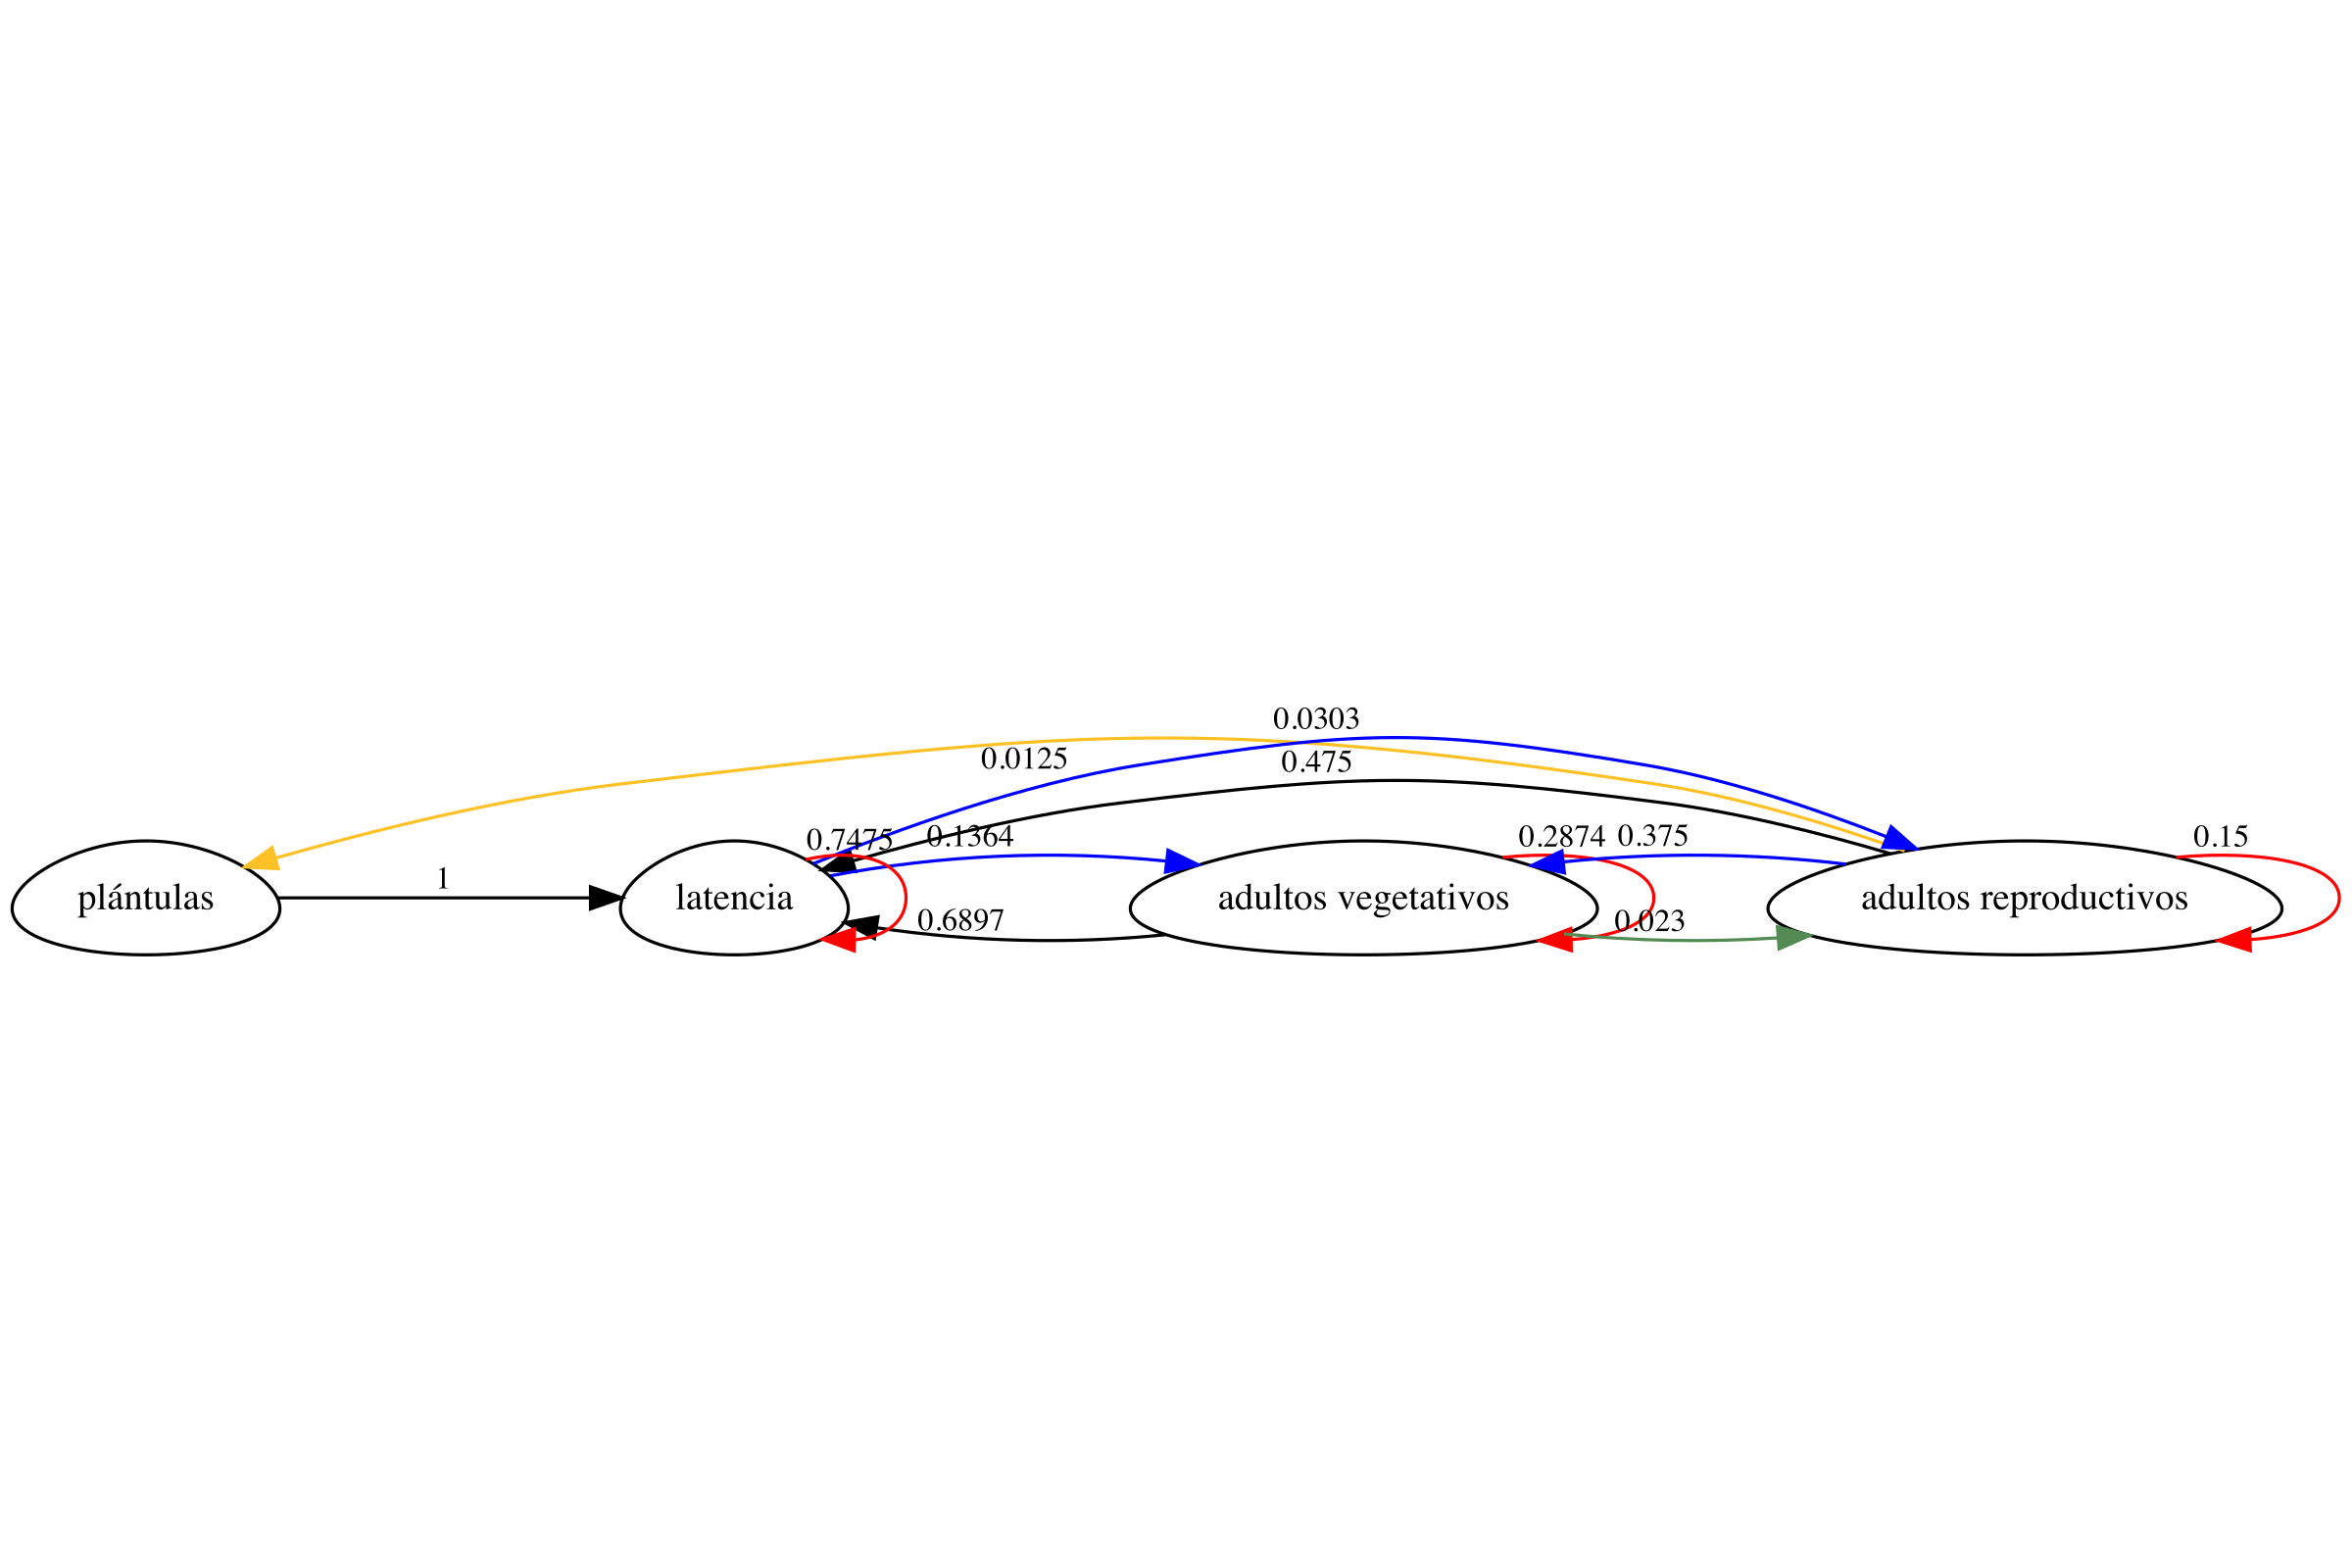
\includegraphics[width=8in,height=\textheight,keepaspectratio]{./images/CV7Prasophyllum_correctum.png}

\subsubsection{\texorpdfstring{\emph{Ophrys
sphegodes}}{Ophrys sphegodes}}\label{ophrys-sphegodes}

En el trabajo de Waite y Hutchings 1991 con \emph{Ophrys sphegodes} se
recolectaron datos de la etapa vegetativa, plantas en flor y latencia de
uno y dos años; por consecuencia, la historia de vida está representada
por 4 etapas. Los datos provienen de la figura 1 y la tabla 3b (periodo
de herbivoría por oveja) de la publicación de (Waite \& Hutchings,
1991). En este caso, se hacen análisis para determinar cuál es la
probabilidad de que un individuo con latencia vegetativa múltiple (uno o
dos años) esté vivo, al comparar poblaciones que están sujetas a la
herbivoría por ovejas o ganado.

Dado que el análisis se enfoca en la sobrevivencia, en el estudio no se
incluye la reproducción (no hay línea amarilla). Las etapas que pasen a
latente el siguiente año se señalan en azul, las que se quedan en la
misma etapa están en rojo, mientras que en verde el tránsito a una etapa
no latente.

\begin{Shaded}
\begin{Highlighting}[]
\NormalTok{G1 }\OtherTok{\textless{}{-}} \FunctionTok{matrix}\NormalTok{(}\FunctionTok{c}\NormalTok{(}\FloatTok{0.0080}\NormalTok{, }\FloatTok{0.0184}\NormalTok{, }\FloatTok{0.0149}\NormalTok{, }\FloatTok{0.0148}\NormalTok{,}
               \FloatTok{0.0180}\NormalTok{, }\FloatTok{0.4249}\NormalTok{, }\FloatTok{0.1214}\NormalTok{, }\FloatTok{0.1214}\NormalTok{,}
               \FloatTok{0.1853}\NormalTok{, }\FloatTok{0.2770}\NormalTok{, }\DecValTok{0}\NormalTok{,      }\DecValTok{0}\NormalTok{,}
               \DecValTok{0}\NormalTok{,      }\DecValTok{0}\NormalTok{,      }\FloatTok{0.3050}\NormalTok{, }\DecValTok{0}\NormalTok{),}
             \AttributeTok{byrow =} \ConstantTok{TRUE}\NormalTok{, }\AttributeTok{ncol =} \DecValTok{4}\NormalTok{)}
\NormalTok{etapas\_Op }\OtherTok{\textless{}{-}} \FunctionTok{c}\NormalTok{(}\StringTok{"Vegetativa"}\NormalTok{, }\StringTok{"Ind. con Flores"}\NormalTok{, }\StringTok{"Latencia año 1"}\NormalTok{, }\StringTok{"Latencia año 2"}\NormalTok{)}
\NormalTok{cols      }\OtherTok{\textless{}{-}} \FunctionTok{c}\NormalTok{(}\StringTok{"red"}\NormalTok{,}\StringTok{"PaleGreen4"}\NormalTok{,}\StringTok{"blue"}\NormalTok{,}\StringTok{"PaleGreen4"}\NormalTok{,}\StringTok{"red"}\NormalTok{,}\StringTok{"blue"}\NormalTok{,}
               \StringTok{"PaleGreen4"}\NormalTok{,}\StringTok{"PaleGreen4"}\NormalTok{,}\StringTok{"blue"}\NormalTok{,}\StringTok{"PaleGreen4"}\NormalTok{,}\StringTok{"PaleGreen4"}\NormalTok{)}

\NormalTok{ne  }\OtherTok{\textless{}{-}} \FunctionTok{make\_nodes\_edges}\NormalTok{(etapas\_Op, G1, cols, }\AttributeTok{minlen\_scale =} \DecValTok{2}\NormalTok{, }\AttributeTok{digits =} \DecValTok{4}\NormalTok{, }\AttributeTok{fontsize =} \DecValTok{10}\NormalTok{)}
\NormalTok{dot }\OtherTok{\textless{}{-}} \FunctionTok{build\_dot}\NormalTok{(ne}\SpecialCharTok{$}\NormalTok{nodes, ne}\SpecialCharTok{$}\NormalTok{edges, }\AttributeTok{title =} \ConstantTok{NULL}\NormalTok{)}

\FunctionTok{render\_dual}\NormalTok{(dot, }\StringTok{"images/CV8\_Ophrys.png"}\NormalTok{)}
\end{Highlighting}
\end{Shaded}

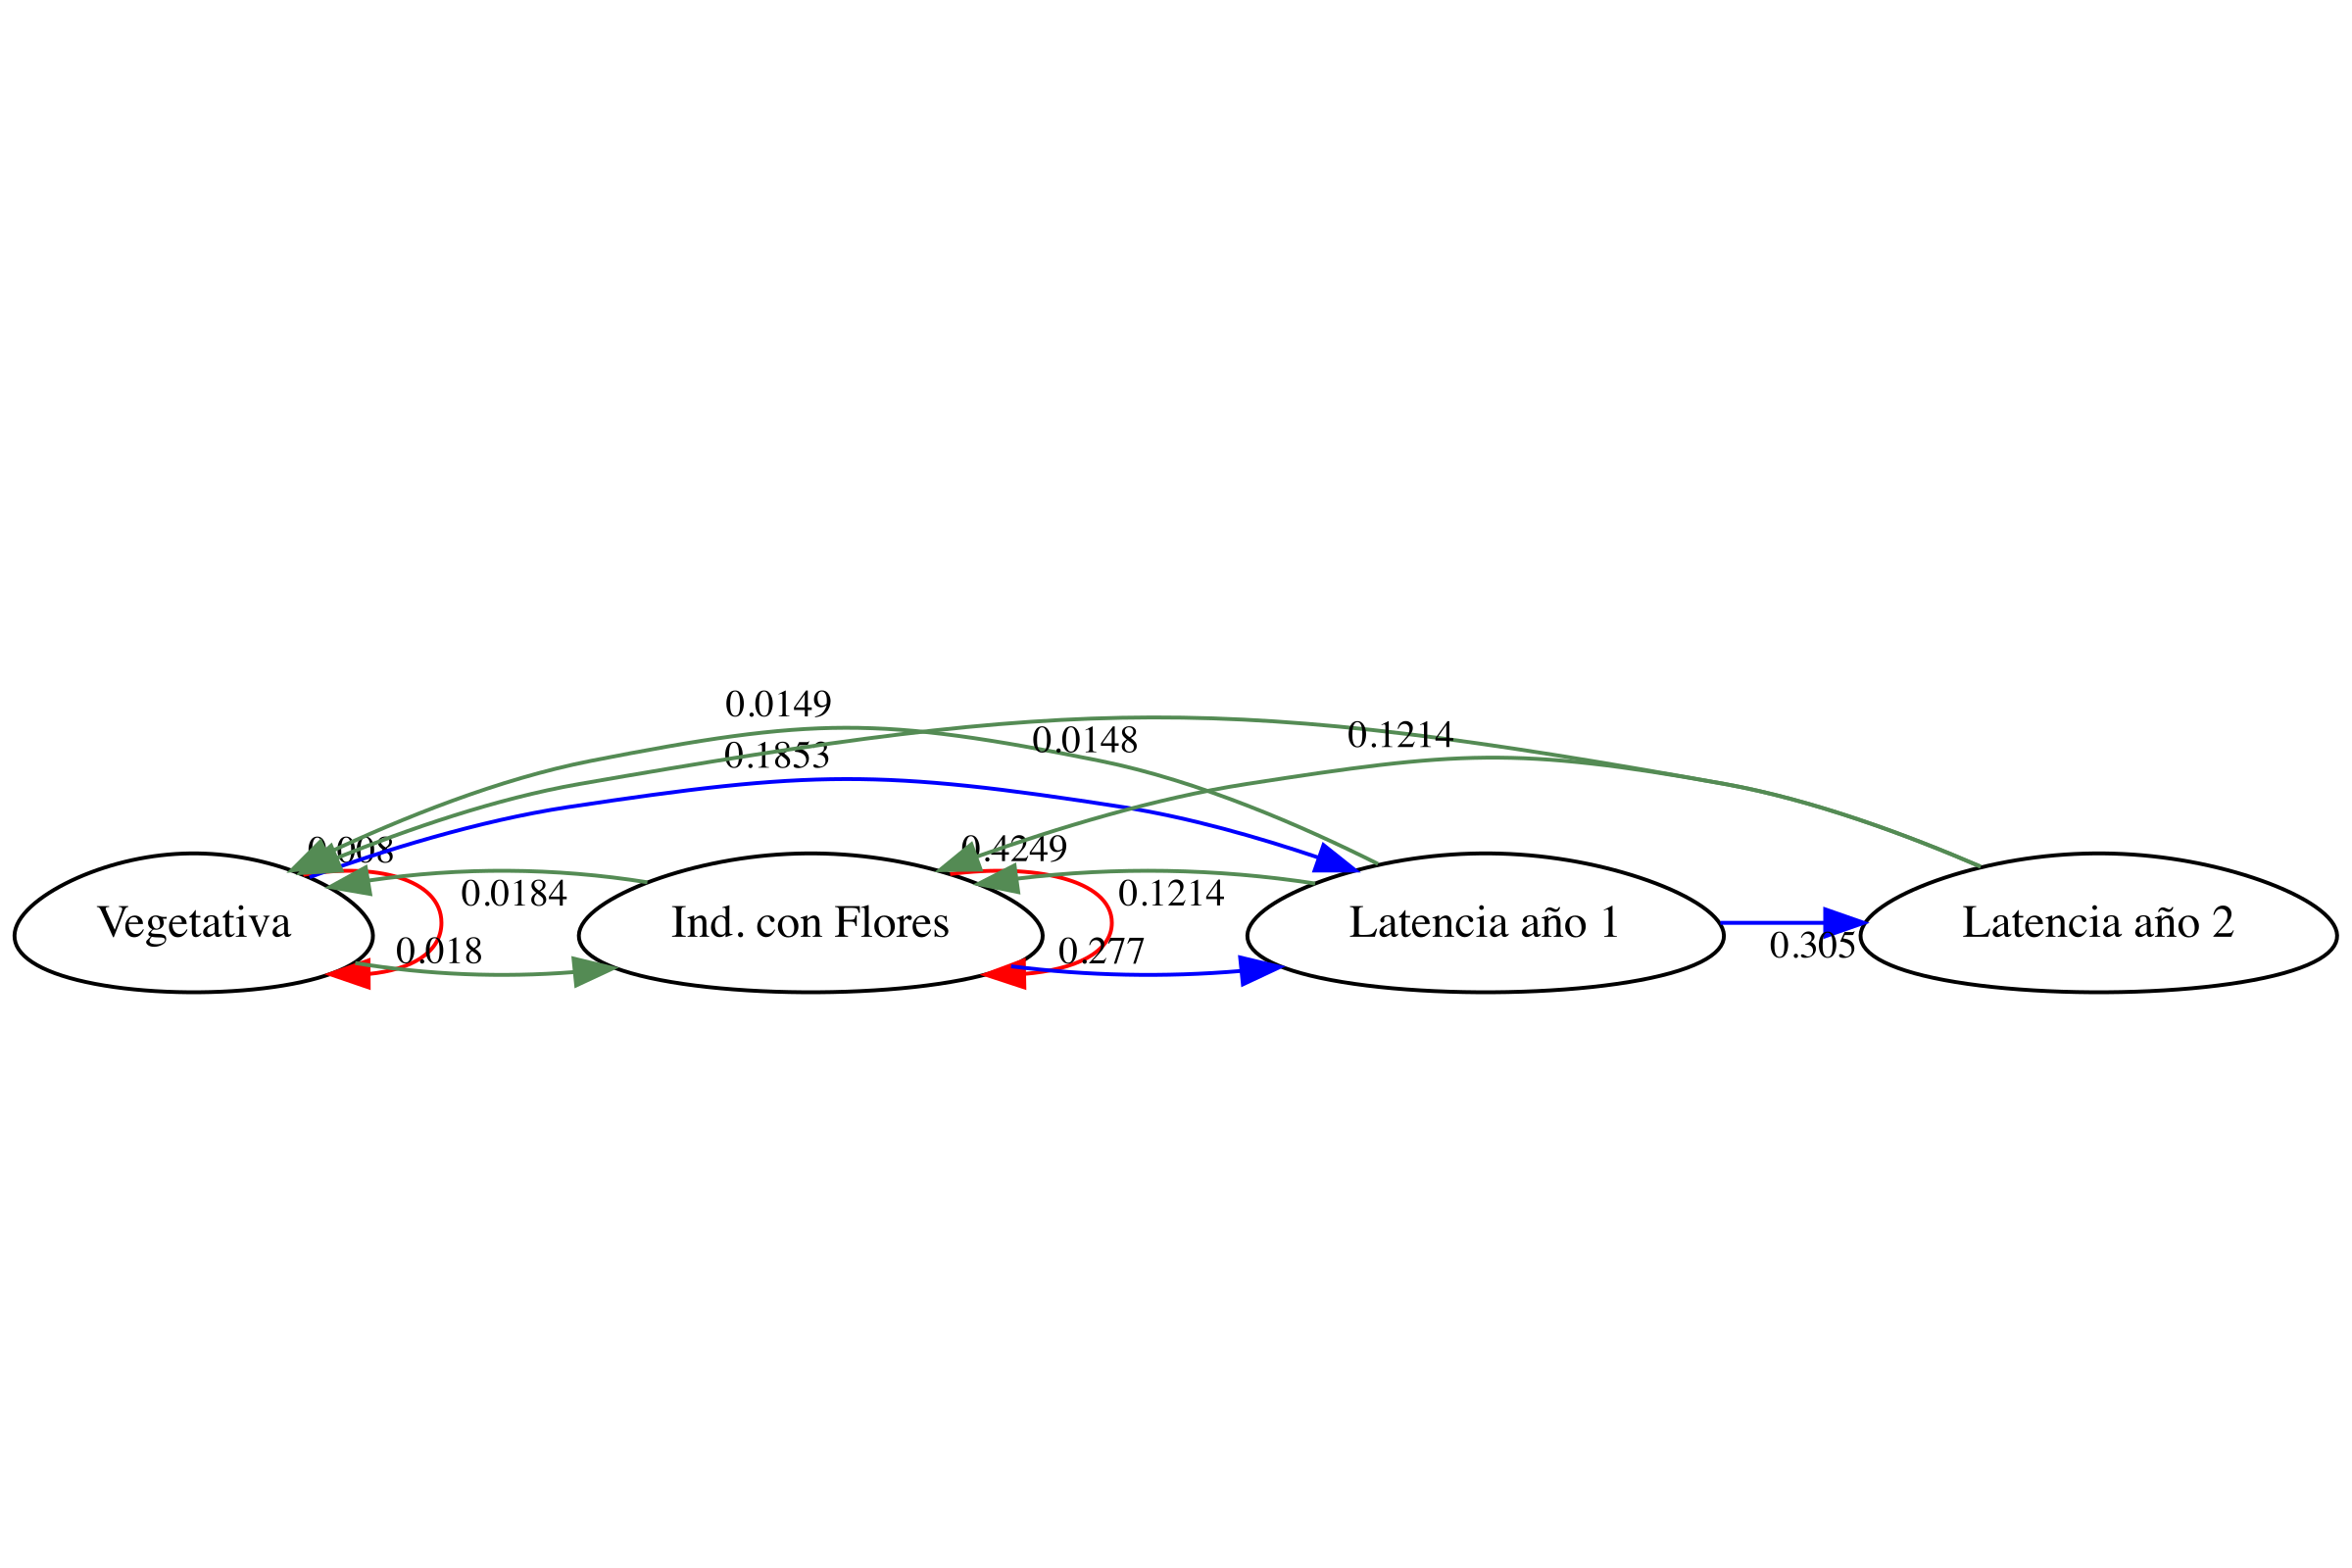
\includegraphics[width=8in,height=\textheight,keepaspectratio]{./images/CV8_Ophrys.png}

\subsubsection{\texorpdfstring{\emph{Cypripedium parviflorum},
\emph{Epipactis atrorubens} y \emph{Orchis
purpurea}}{Cypripedium parviflorum, Epipactis atrorubens y Orchis purpurea}}\label{cypripedium-parviflorum-epipactis-atrorubens-y-orchis-purpurea}

\begin{figure}[H]

{\centering \pandocbounded{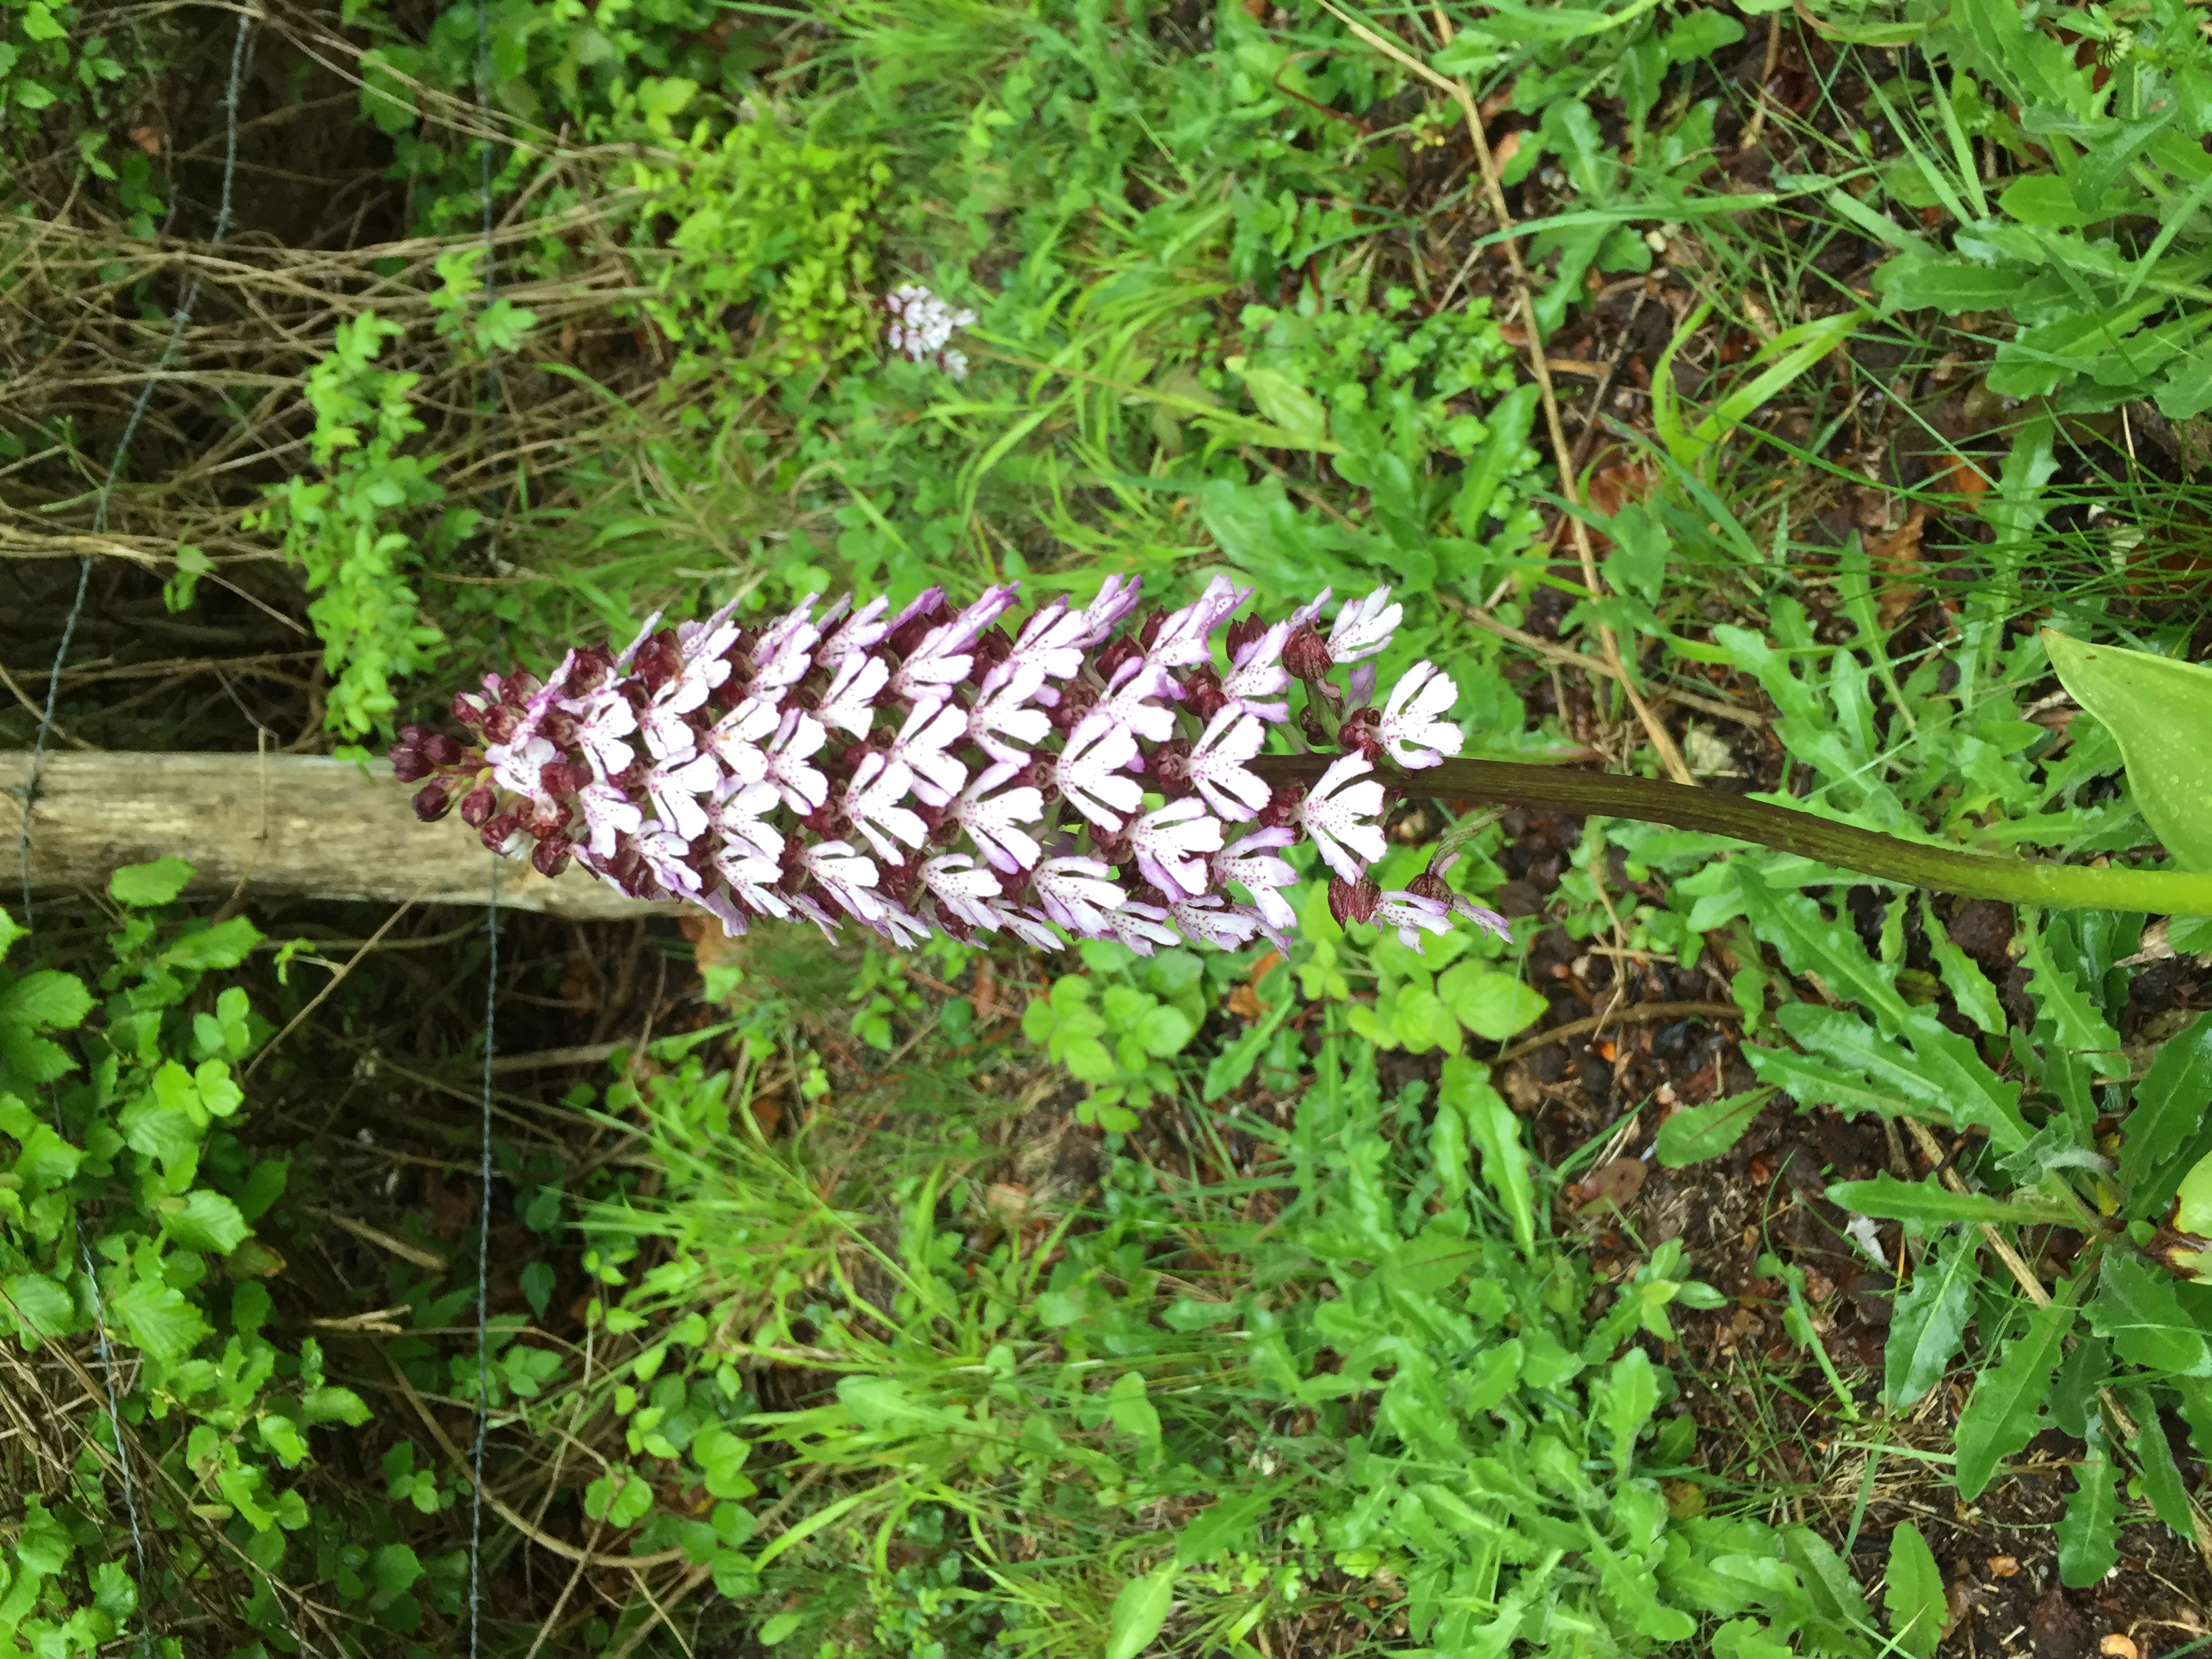
\includegraphics[keepaspectratio]{images/Orchis_purpurea_1_Hans_Jacquemyn.jpg}}

}

\caption{\emph{Orchis purpurea}. Foto: Hans Jacquemyn}

\end{figure}%

La dimensiones de la matriz y la cantidad de etapas o años incluidos en
un análisis depende de múltiples factores. Cuando se trabaja con datos
de campo, el acceso a individuos de cada etapa del ciclo de vida es, sin
duda, un factor determinante. En la revisión de la publicaciones sobre
orquídeas se encuentran análisis matriciales que varían entre 3 y 29
etapas de desarrollo, en promedio 5.6 etapas (desv. estándar de 3.2). El
trabajo con mayor número de etapas es el de (Shefferson, Warren \&
Pulliam, 2014), que utilizó 29 en \emph{Cypripedium parviflorum} var.
\emph{parviflorum}.

El costo de pasar a una fase latente después de diferentes etapas se
evaluó en \emph{Epipactis atrorubens}. En este análisis se definieron 11
estados, considerando la posibilidad de entrar en latencia vegetativa
desde todas estas fases emergentes (Jäkäläniemi et~al., 2011). En
\emph{Orchis purpurea}, los autores modelaron el diagrama del ciclo de
vida, definiendo 6 etapas de desarrollo: protocormos, tubérculos,
plántulas, juveniles (más de un año y menos de 3 hojas), plantas sin
flores (más de 3 hojas) y plantas con flores, a continuación se presenta
la matriz correspondiente tomada de (Jacquemyn, Brys \& Jongejans,
2010). La transiciones a una etapa subsiguiente se señalan en verde, en
violeta las transiciones a una etapa más pequeña y la reproducción en
amarillo. En este ciclo de vida las etapas de protocormos, tubérculos y
plántulas son de un año cada una. Si estos individuos no crecen a la
próxima etapa se supone que fallecieron.

\begin{center}\rule{0.5\linewidth}{0.5pt}\end{center}

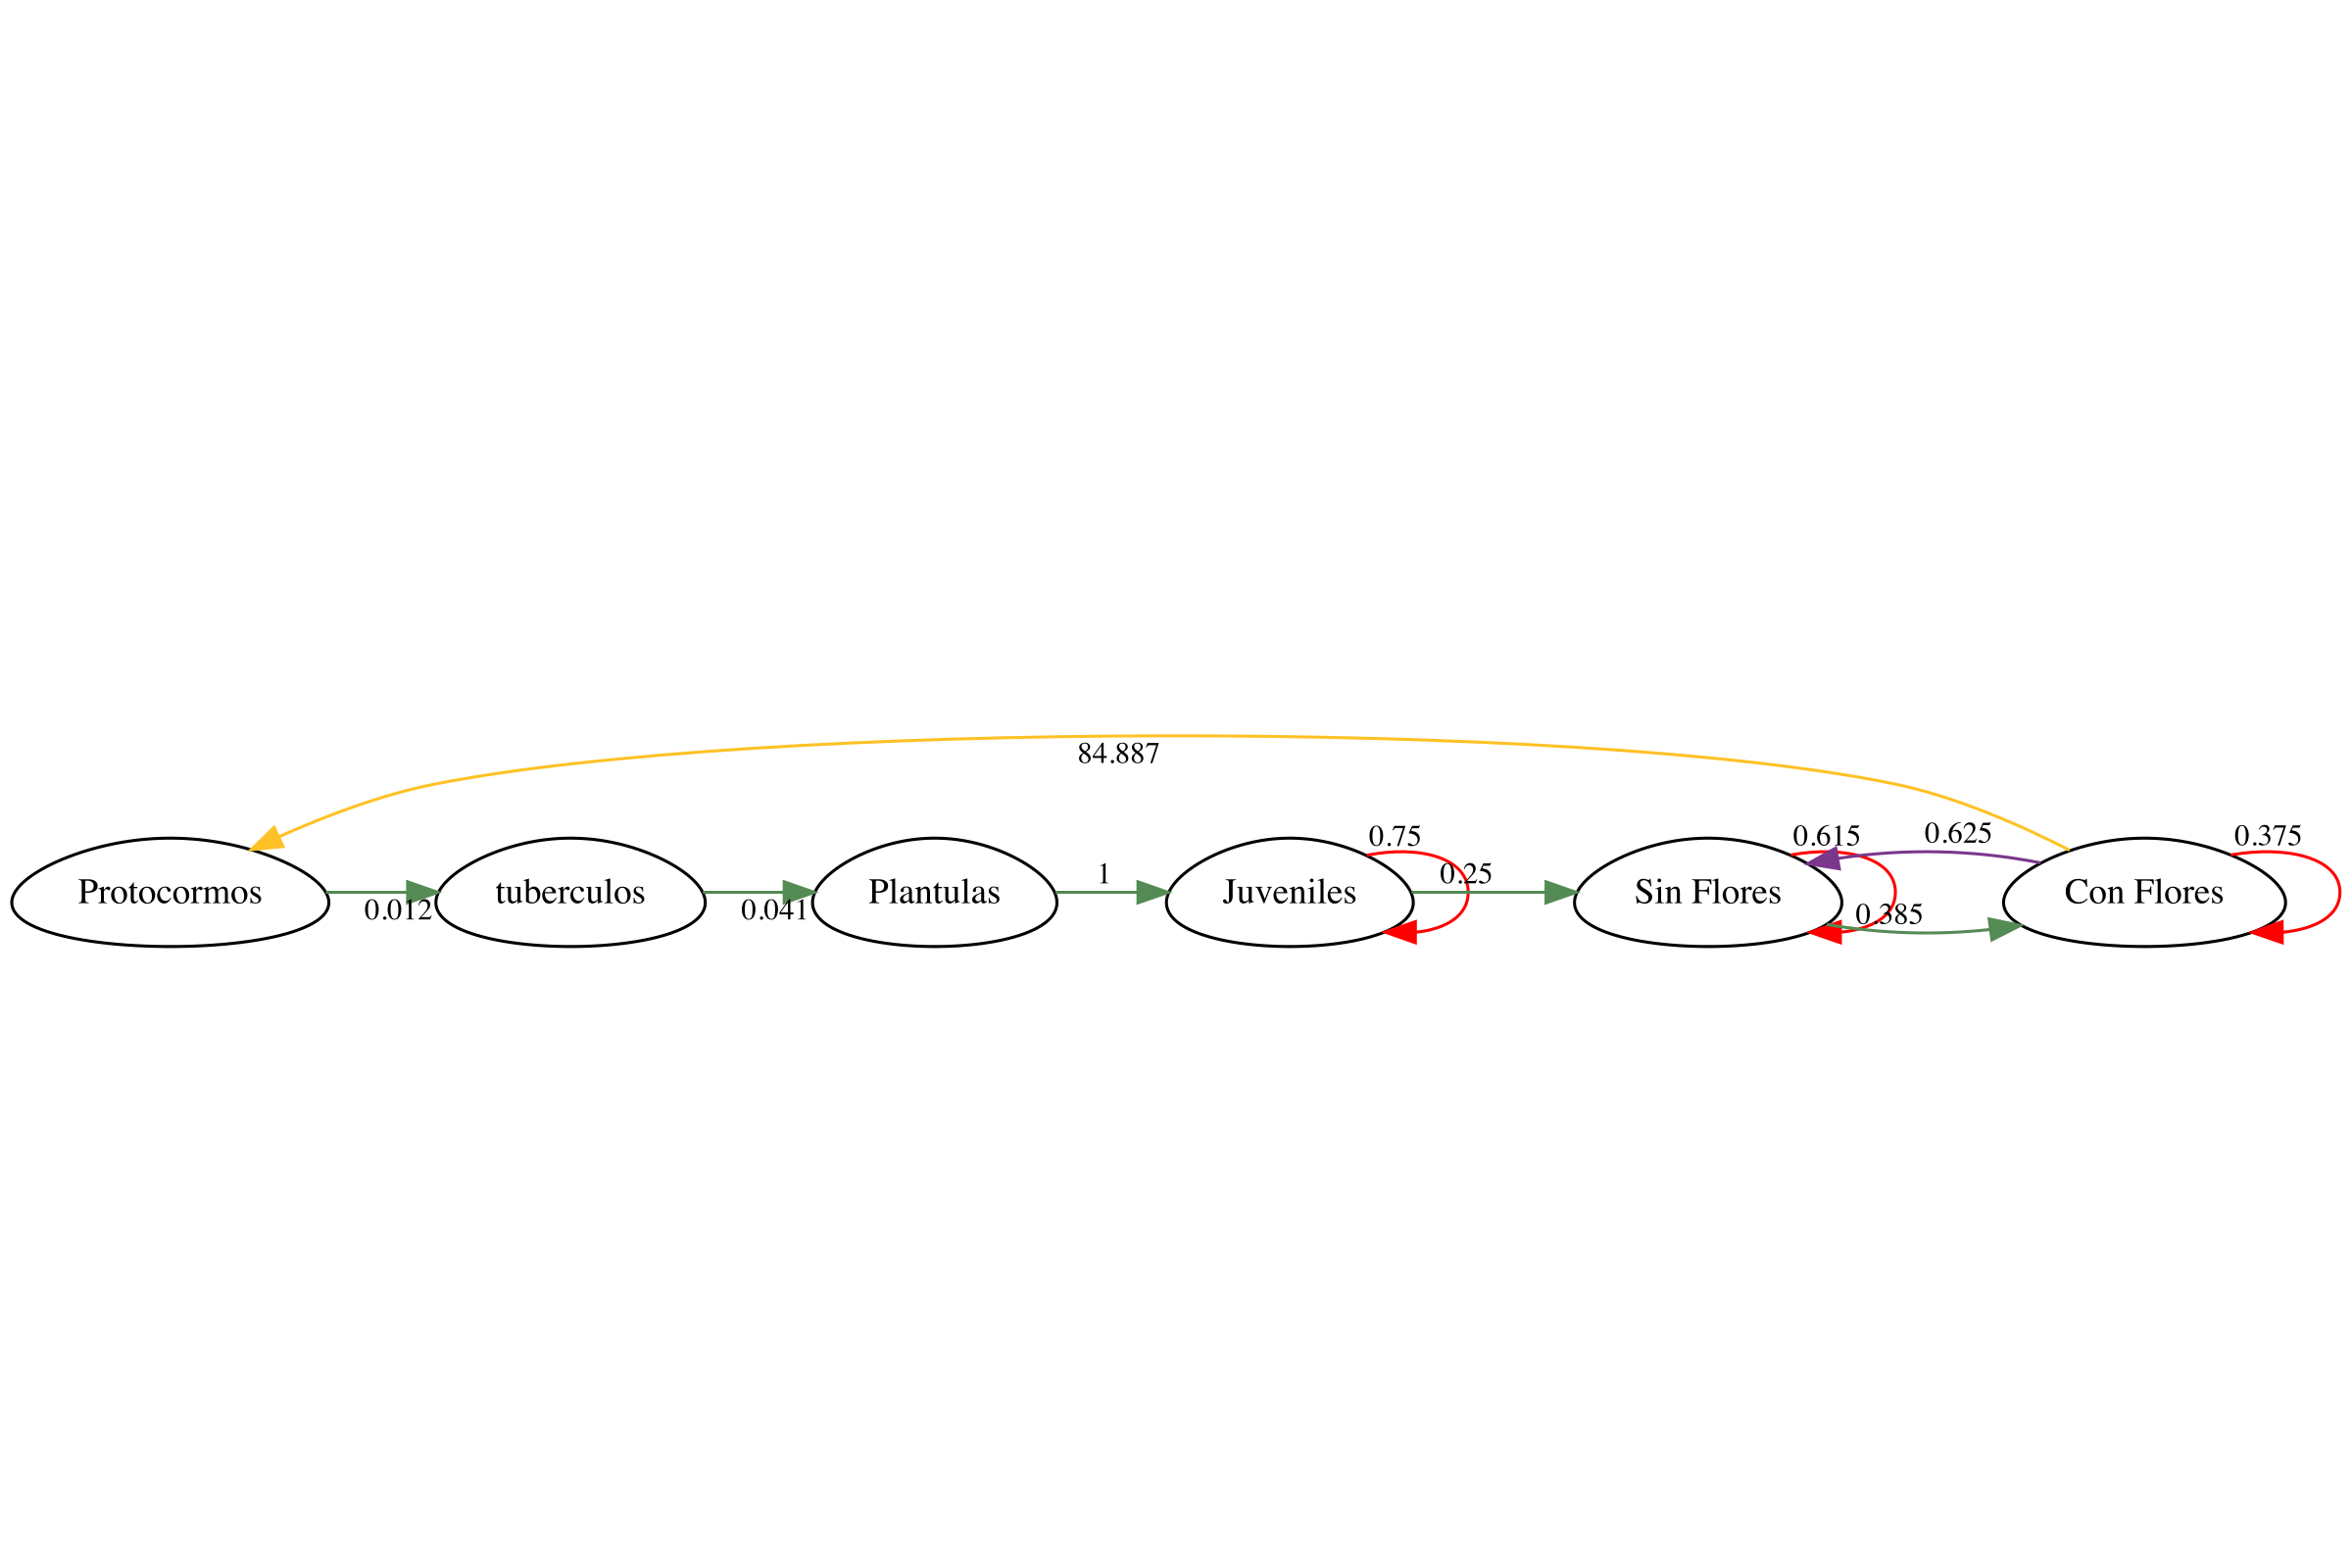
\includegraphics[width=8in,height=\textheight,keepaspectratio]{./images/CV9_Os.png}

\begin{figure}[H]

{\centering 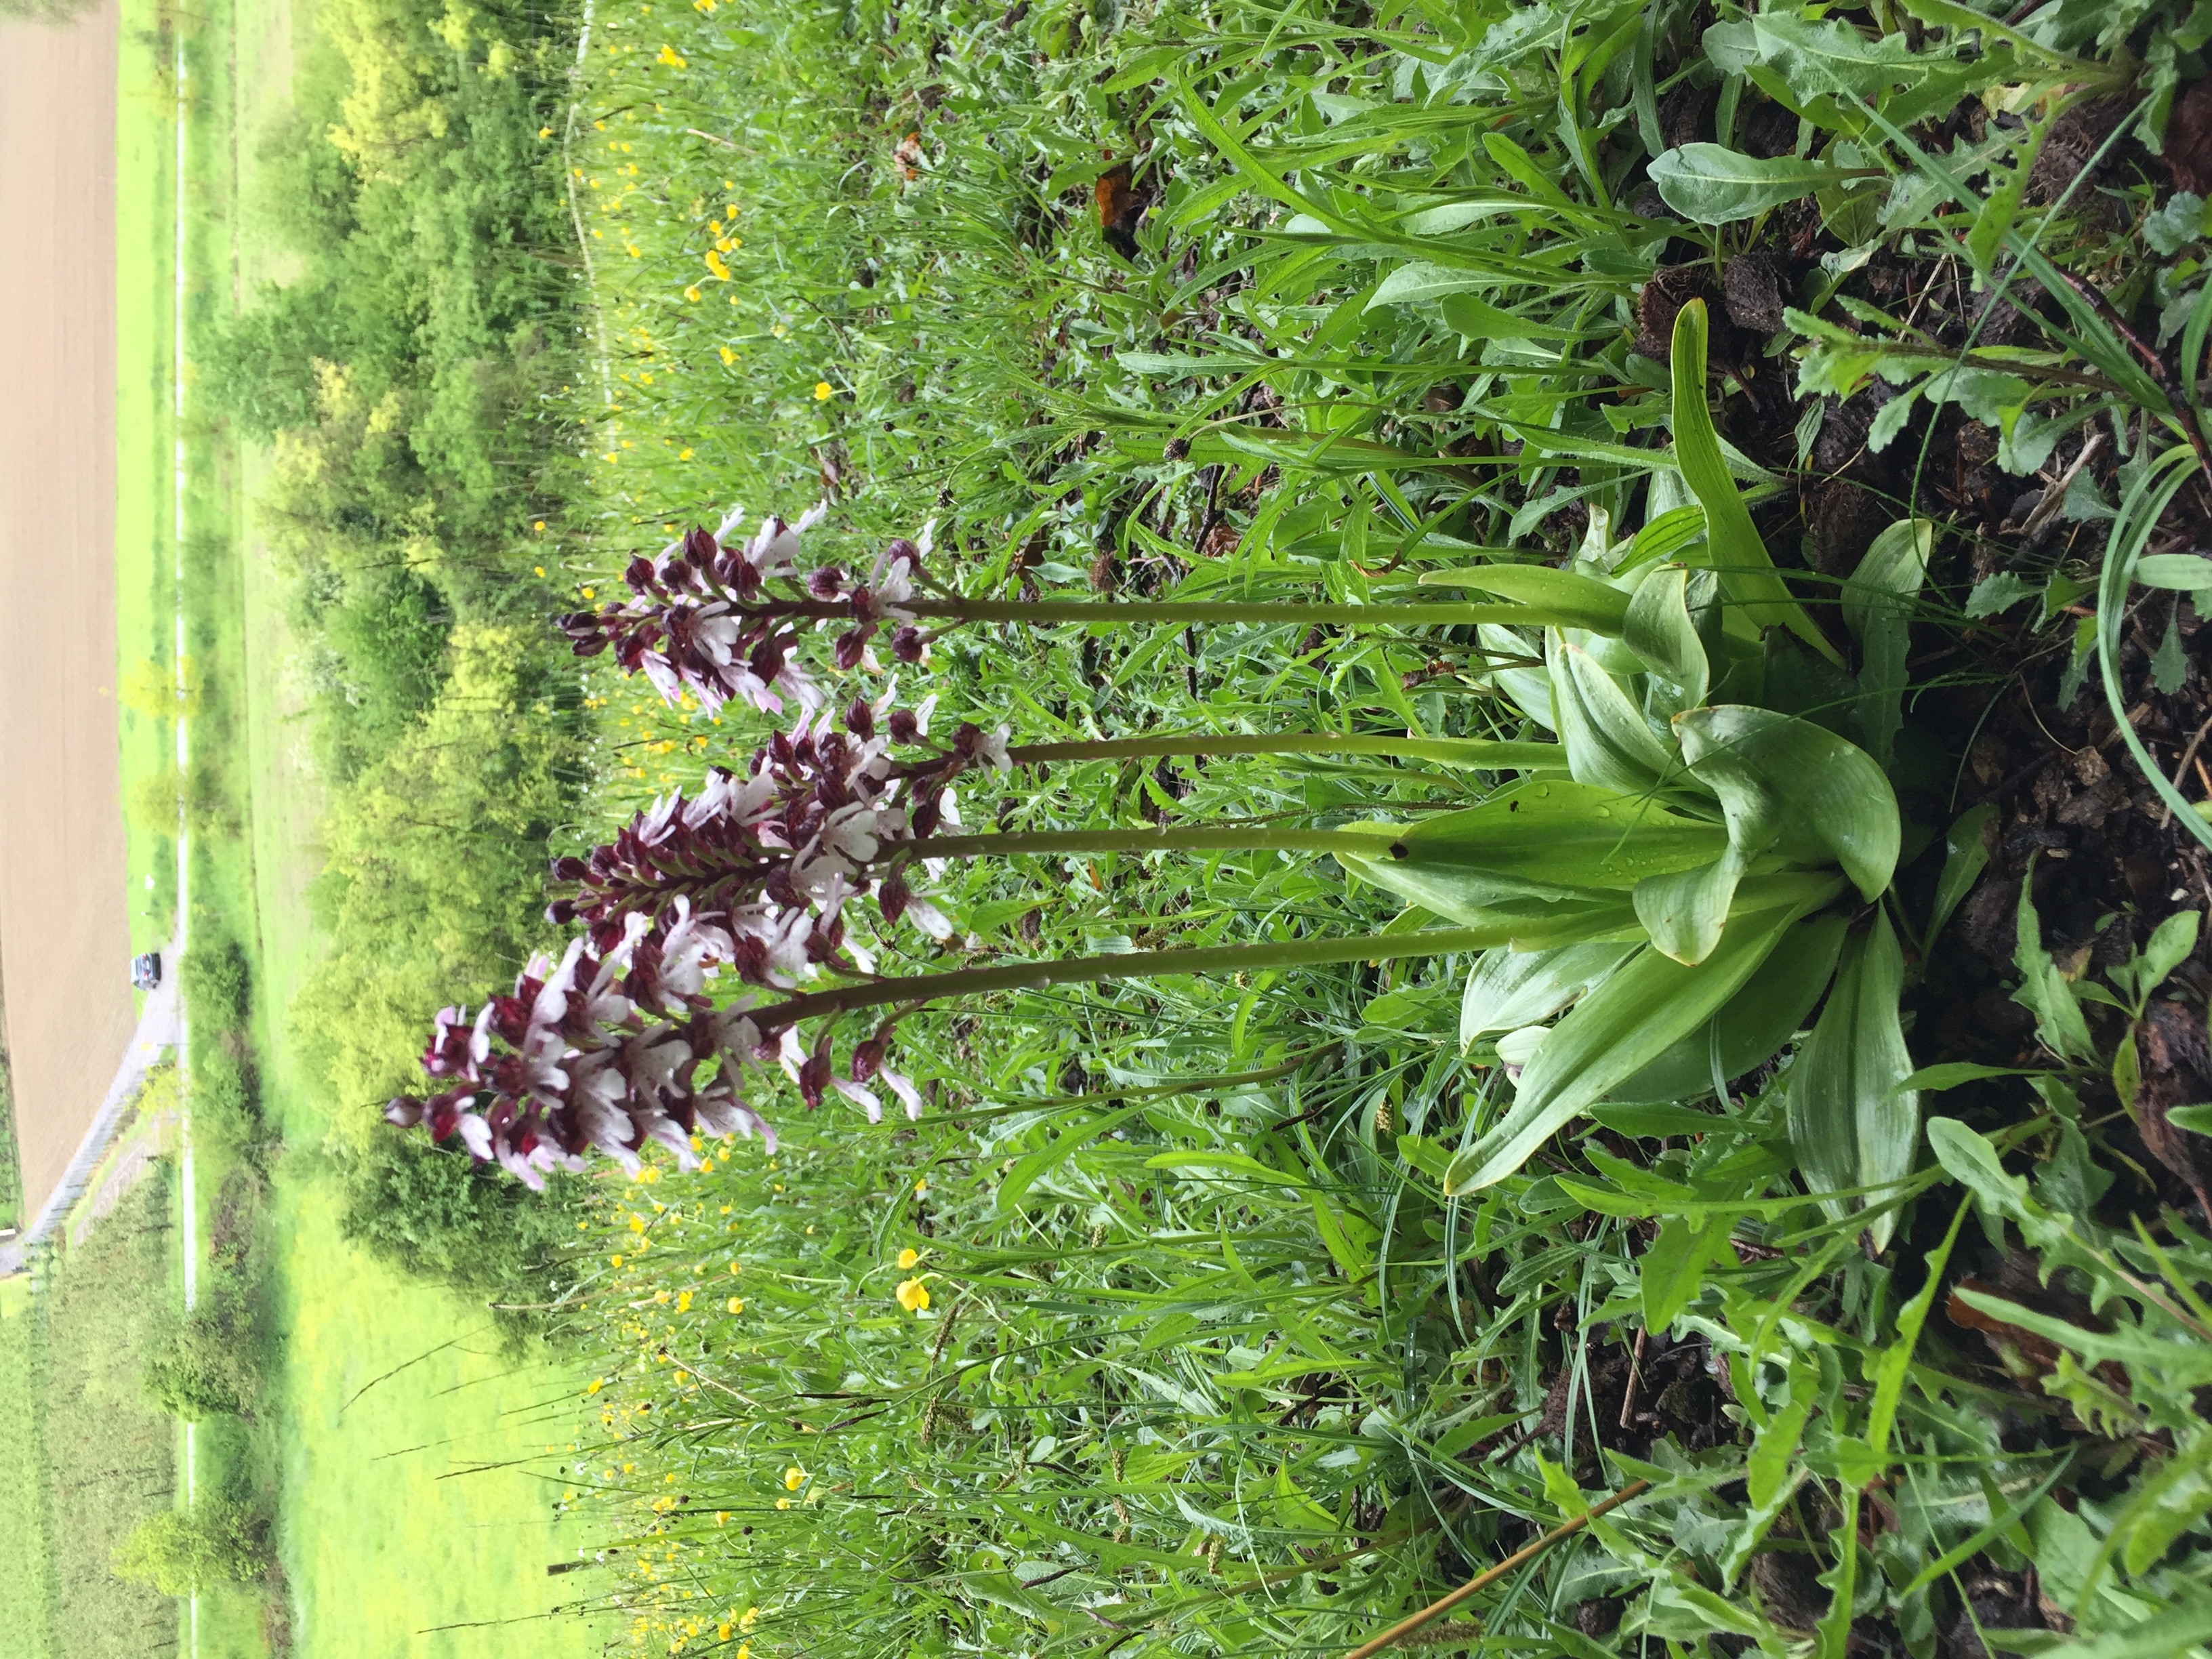
\includegraphics[width=0.6\linewidth,height=\textheight,keepaspectratio]{images/Orchis_purpurea_2_Hans_Jacquemyn.jpg}

}

\caption{\emph{Orchis purpurea}. Foto: Hans Jacquemyn}

\end{figure}%

\begin{center}\rule{0.5\linewidth}{0.5pt}\end{center}

\subsection{Ejemplo de un ciclo de vida incompleto (y biológicamente
erróneo)}\label{ejemplo-de-un-ciclo-de-vida-incompleto-y-bioluxf3gicamente-erruxf3neo}

\begin{tcolorbox}[enhanced jigsaw, arc=.35mm, bottomrule=.15mm, bottomtitle=1mm, breakable, colback=white, colbacktitle=quarto-callout-warning-color!10!white, colframe=quarto-callout-warning-color-frame, coltitle=black, left=2mm, leftrule=.75mm, opacityback=0, opacitybacktitle=0.6, rightrule=.15mm, title=\textcolor{quarto-callout-warning-color}{\faExclamationTriangle}\hspace{0.5em}{Advertencia}, titlerule=0mm, toprule=.15mm, toptitle=1mm]

\textbf{Tres errores típicos en datos de campo ---y por qué importan.}

\begin{itemize}
\tightlist
\item
  \textbf{Etapas sin mortalidad} (suma de columna = 1 sin pérdidas):
  biológicamente irreal salvo en casos de latencia perfecta.
\item
  \textbf{Etapas con mortalidad total} (todos los individuos mueren
  entre intervalos): rompe la cadena del ciclo y borra una transición
  real que probablemente sí ocurre con baja frecuencia.
\item
  \textbf{Permanencia perpetua} (un estadio nunca contribuye a otros ni
  muere): elimina toda dinámica del estadio.
\end{itemize}

Estos errores suelen aparecer cuando el tamaño de muestra es pequeño o
las transiciones son raras. Antes de aceptar la matriz, conviene revisar
el diagrama del ciclo de vida y preguntarse: ¿es biológicamente
plausible que esta entrada sea exactamente cero?

\end{tcolorbox}

La importancia de este capítulo radica en reconocer la diferencia entre
la historia de vida real de un organismo y la información que se puede
recolectar en el campo. En los estudios poblacionales de orquídeas, dos
desafíos en su investigación y muestreo son la dificultad, por un lado,
de rastrear y hacer una seguimiento de las semillas en el campo y, por
otro, el determinar los sitios adecuados para su germinación (sitios
seguros). Este segundo aspecto implica considerar la presencia de
micorrizas, cuya asociación con las semillas es determinante para su
germinación. Estas etapas tempranas del ciclo de vida de las orquídeas
suelen estar rodeadas de gran incertidumbre, lo que limita los análisis
e interpretaciones de su evolución y conservación.

Además de los anteriores, existen otros problemas. La recolección de
datos en campo puede ser irreal en el contexto de la historia de vida y
la base matemática del modelo representado. Para más detalles ver el
capítulo \href{122-Impacto_de_Datos_sin_Sentido.qmd}{Impacto de datos
sin sentido}. Por ejemplo, en la Figura~\ref{fig-cv10} aparecen tres
errores comunes durante la recolección de datos de la historia de vida
de una especie. El primero es que no hay mortalidad de los individuos en
una de las etapas (juveniles), el segundo es que todos los individuos se
mueren (plántulas) y el tercero es que los individuos se mantienen en la
misma etapa de desarrollo (adultos) y no hay muerte. Dada la muerte de
las plántulas, no hay flecha que una a este estado con otros estados. La
falta de continuidad o conexión entre las etapas del ciclo de vida son
errores que ocurren típicamente cuando el tamaño de muestra es pequeño o
la probabilidad de transición es rara o poco frecuente; por ejemplo, los
árboles grandes no fallecen. Estos son los tres errores típicos a los
que nos enfrentamos cuando se lleva a cabo un análisis de dinámica
poblacional en especies con transiciones poco comunes.

\begin{Shaded}
\begin{Highlighting}[]
\NormalTok{matA\_incom }\OtherTok{\textless{}{-}} \FunctionTok{rbind}\NormalTok{(}
  \FunctionTok{c}\NormalTok{(}\FloatTok{0.0}\NormalTok{, }\FloatTok{0.0}\NormalTok{, }\FloatTok{3.2}\NormalTok{),}
  \FunctionTok{c}\NormalTok{(}\FloatTok{0.0}\NormalTok{, }\FloatTok{1.0}\NormalTok{, }\FloatTok{0.1}\NormalTok{),}
  \FunctionTok{c}\NormalTok{(}\FloatTok{0.0}\NormalTok{, }\FloatTok{0.0}\NormalTok{, }\FloatTok{0.9}\NormalTok{)}
\NormalTok{)}
\NormalTok{etapas\_incom }\OtherTok{\textless{}{-}} \FunctionTok{c}\NormalTok{(}\StringTok{"plántula"}\NormalTok{, }\StringTok{"juvenil"}\NormalTok{, }\StringTok{"adulto"}\NormalTok{)}
\NormalTok{cols         }\OtherTok{\textless{}{-}} \FunctionTok{c}\NormalTok{(}\StringTok{"red"}\NormalTok{,}\StringTok{"Goldenrod1"}\NormalTok{,}\StringTok{"MediumOrchid4"}\NormalTok{,}\StringTok{"red"}\NormalTok{)}

\NormalTok{ne  }\OtherTok{\textless{}{-}} \FunctionTok{make\_nodes\_edges}\NormalTok{(etapas\_incom, matA\_incom, cols, }\AttributeTok{minlen\_scale =} \DecValTok{3}\NormalTok{, }\AttributeTok{digits =} \DecValTok{3}\NormalTok{, }\AttributeTok{fontsize =} \DecValTok{10}\NormalTok{)}
\NormalTok{dot }\OtherTok{\textless{}{-}} \FunctionTok{build\_dot}\NormalTok{(ne}\SpecialCharTok{$}\NormalTok{nodes, ne}\SpecialCharTok{$}\NormalTok{edges, }\AttributeTok{title =} \ConstantTok{NULL}\NormalTok{)}

\FunctionTok{render\_dual}\NormalTok{(dot, }\StringTok{"images/CV10.png"}\NormalTok{)}
\end{Highlighting}
\end{Shaded}

\begin{figure}[H]

\centering{

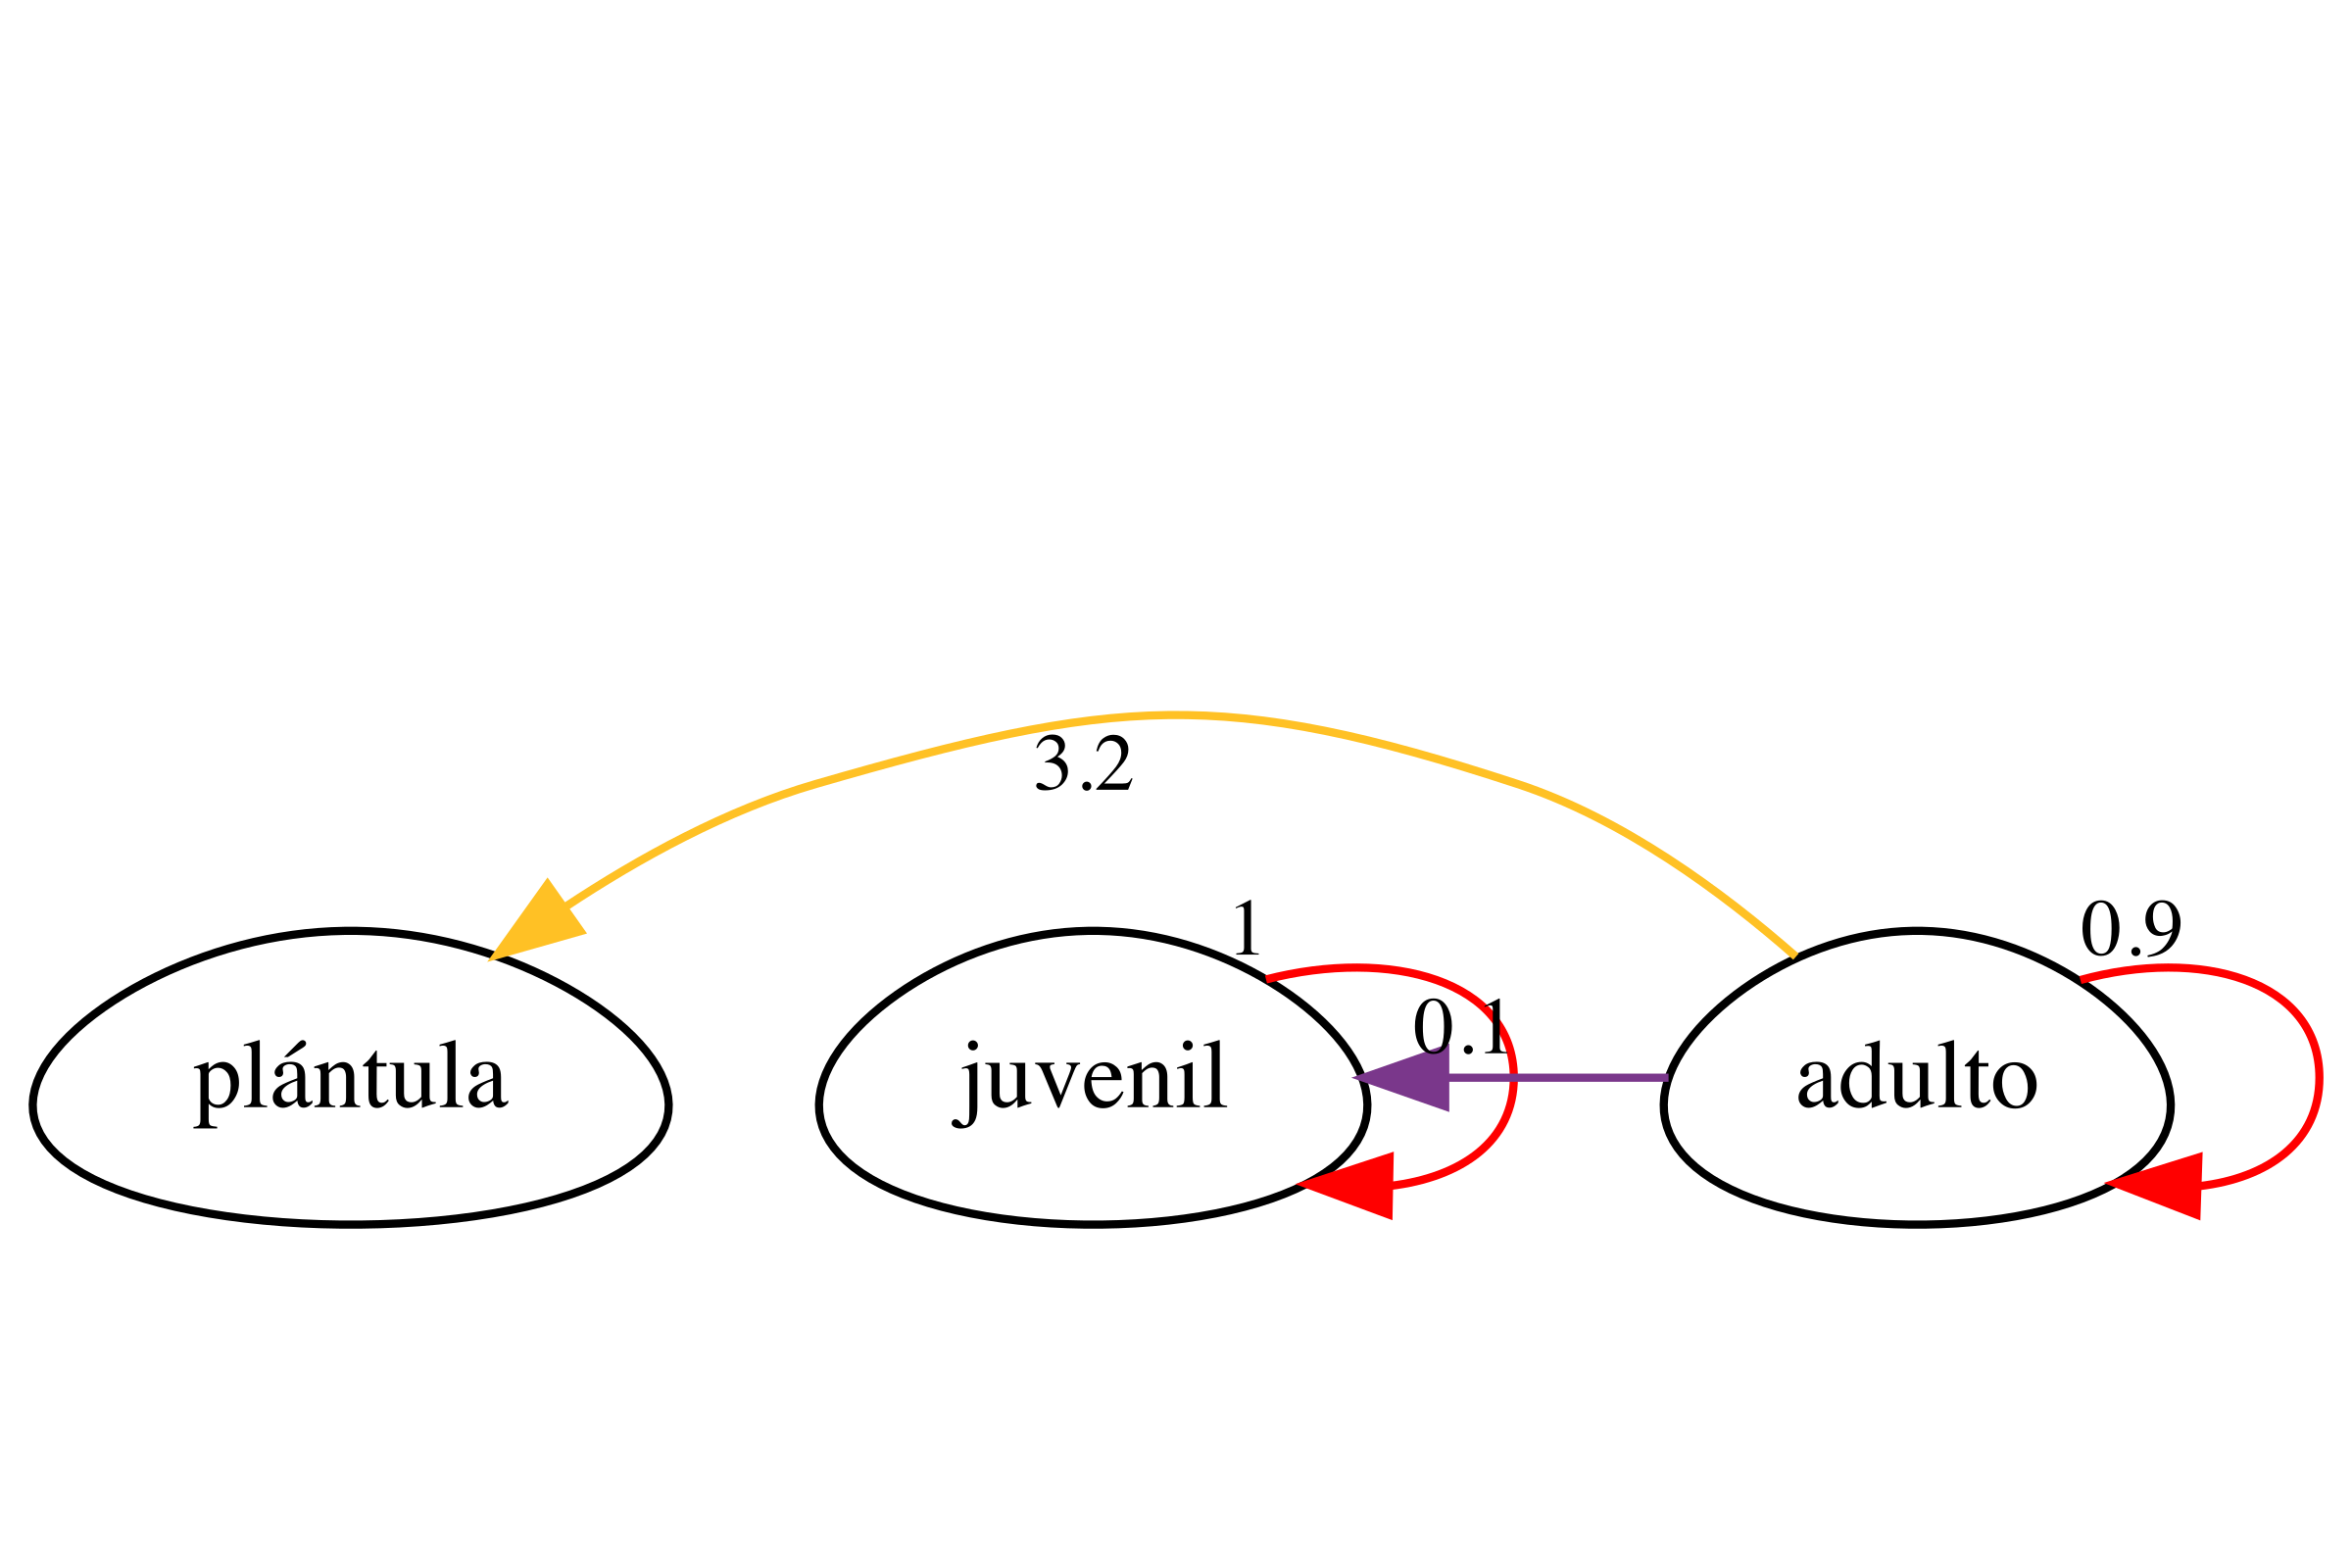
\includegraphics[width=8in,height=\textheight,keepaspectratio]{./images/CV10.png}

}

\caption{\label{fig-cv10}Ejemplo de un ciclo de vida incompleto con tres
errores típicos durante la recolección de datos: ausencia de mortalidad
en juveniles, mortalidad total de plántulas y permanencia perpetua en
adultos sin muerte.}

\end{figure}%

\begin{center}\rule{0.5\linewidth}{0.5pt}\end{center}

\section{Ejemplo de un diagrama de un ciclo de vida usando el paquete
ggplot}\label{ejemplo-de-un-diagrama-de-un-ciclo-de-vida-usando-el-paquete-ggplot}

En la graficación del ciclo de vida podemos usar otro paquete de R,
\texttt{Rage} (ver Figura~\ref{fig-cv11}). La diferencia es que no se
pueden cambiar los colores de las líneas y los nodos (círculos que
representan los estados de desarrollo). Esta es una opción más sencilla
para crear diagramas de ciclo de vida, además de ser práctica para
publicaciones donde no se necesita cambiar los colores de las líneas y
nodos.

\begin{figure}

\centering{

\pandocbounded{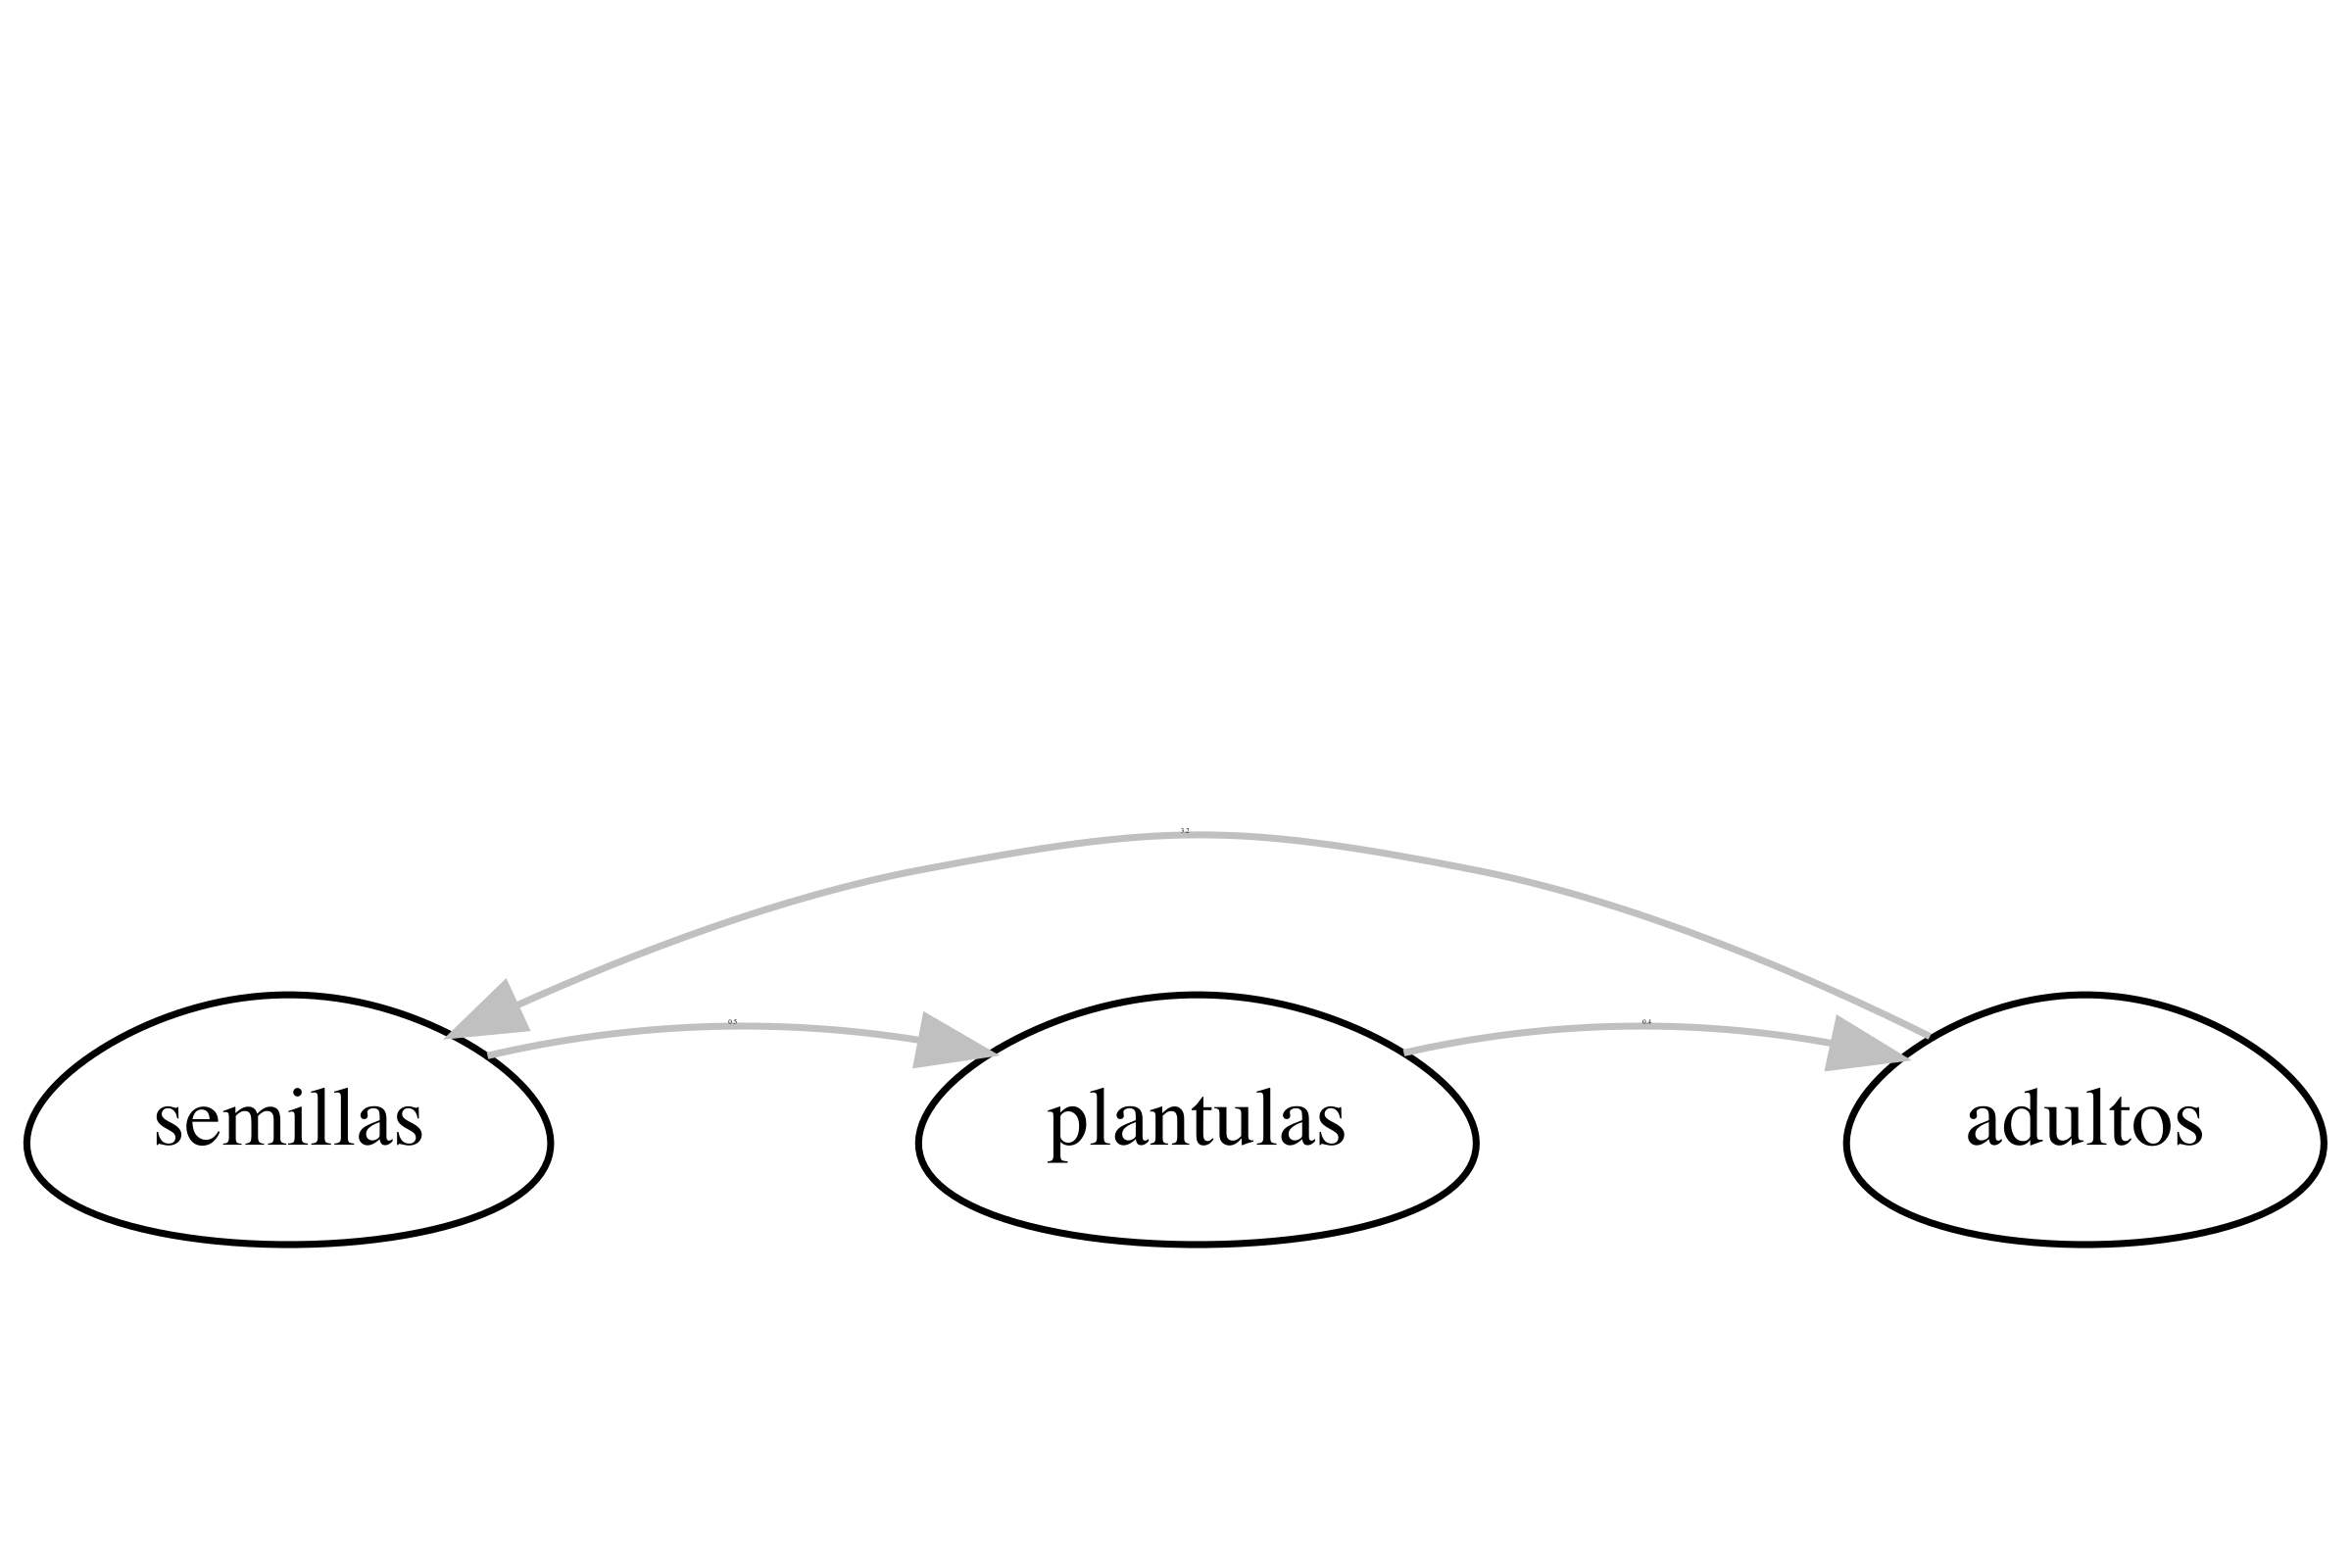
\includegraphics[keepaspectratio]{figs/CV11_Rage_plot.png}}

}

\caption{\label{fig-cv11}Diagrama de ciclo de vida construido con el
paquete \texttt{Rage}.}

\end{figure}%

\bookmarksetup{startatroot}

\chapter{Recopilar datos en el campo}\label{Recopilacion}

Por: Aucencia Emeterio-Lara, Mariana Hernández-Apolinar y Raymond L.
Tremblay

La recopilación de datos demográficos en el campo constituye la base
empírica de los modelos de dinámica poblacional. Este capítulo presenta
los principios conceptuales y prácticos para diseñar y ejecutar
muestreos de campo que permitan estimar de forma coherente las tasas
vitales utilizadas en modelos poblacionales estructurados.

\section{Datos de campo y su vínculo con la dinámica
poblacional}\label{datos-de-campo-y-su-vuxednculo-con-la-dinuxe1mica-poblacional}

Existe una relación crítica entre los modelos de dinámica poblacional y
la calidad y estructura de los datos recolectados en el campo. Las
decisiones tomadas durante el diseño del muestreo ---qué medir, cuándo
medir y a qué escala--- tienen implicaciones directas sobre la
estimación de supervivencia, crecimiento y fecundidad, y por lo tanto
sobre la interpretación de la dinámica poblacional.

En este capítulo se discuten los fundamentos conceptuales de la
recopilación de datos demográficos, destacando la importancia de alinear
los protocolos de campo con la estructura del ciclo de vida representado
en los modelos. Se analiza cómo distintas estrategias de muestreo
influyen en la definición de estadios, en la estimación de transiciones
demográficas y en la construcción posterior de matrices de proyección
poblacional.

Asimismo, se abordan consideraciones prácticas como la frecuencia de
muestreo, el seguimiento individual, la detección de eventos
reproductivos y el manejo de datos faltantes o censurados. Este capítulo
se diferencia de los posteriores porque se centra en el \textbf{origen
empírico} de los parámetros demográficos, estableciendo el puente entre
el trabajo de campo y las herramientas analíticas desarrolladas más
adelante. Una recopilación de datos adecuadamente diseñada es esencial
para garantizar inferencias robustas y proyecciones poblacionales
biológicamente interpretables.

\begin{tcolorbox}[enhanced jigsaw, arc=.35mm, bottomrule=.15mm, bottomtitle=1mm, breakable, colback=white, colbacktitle=quarto-callout-tip-color!10!white, colframe=quarto-callout-tip-color-frame, coltitle=black, left=2mm, leftrule=.75mm, opacityback=0, opacitybacktitle=0.6, rightrule=.15mm, title=\textcolor{quarto-callout-tip-color}{\faLightbulb}\hspace{0.5em}{Recomendación}, titlerule=0mm, toprule=.15mm, toptitle=1mm]

\textbf{Las decisiones de muestreo definen las inferencias posibles.} Lo
que no se mide en el campo no se puede recuperar después. La elección de
etapas, la frecuencia del censo, el tamaño de la muestra y el método de
marcaje determinan qué tasas vitales podrán estimarse y con qué
precisión. Antes de salir al campo, conviene preguntarse: dado el ciclo
de vida hipotético, ¿este protocolo me permitirá estimar todas las
transiciones que necesito para construir la matriz?

\end{tcolorbox}

\section{Diseño de muestreo y protocolos de
campo}\label{diseuxf1o-de-muestreo-y-protocolos-de-campo}

A continuación se describen los métodos y protocolos utilizados para la
recopilación de datos demográficos en el campo, incluyendo ejemplos de
seguimiento individual y medición de tasas vitales.

\subsubsection{Librerías de R requeridas para el siguiente
módulo}\label{libreruxedas-de-r-requeridas-para-el-siguiente-muxf3dulo-2}

\begin{Shaded}
\begin{Highlighting}[]
\FunctionTok{library}\NormalTok{(knitr)}
\FunctionTok{library}\NormalTok{(tidyverse)}
\FunctionTok{library}\NormalTok{(dplyr)}
\FunctionTok{library}\NormalTok{(flextable)}
\FunctionTok{library}\NormalTok{(Rcompadre)}
\end{Highlighting}
\end{Shaded}

\section{Consideraciones para la recolección de datos en
campo}\label{consideraciones-para-la-recolecciuxf3n-de-datos-en-campo}

Con el propósito de evaluar el estado de conservación, los estudios de
dinámica poblacional se enfocan en analizar los cambios en la abundancia
(i.e., número de individuos) y comprender los procesos biológicos y
abióticos que influyen en su variación temporal (Silvertown \&
Charlesworth, 2009). Este capítulo destaca aspectos clave a considerar
al planificar un estudio poblacional en orquídeas, y con el objetivo de
orientar la organización de actividades de campo, garantizar la
consistencia en la toma de datos y minimizar errores durante la
recolección. Los datos de campo constituyen la base para estimar las
transiciones demográficas utilizadas en los modelos poblacionales.

Las recomendaciones abarcan desde elementos biológicos hasta
procedimientos técnicos, incluyendo estrategias de muestreo, métodos de
marcaje (i.e., captura) y seguimiento (i.e., recaptura), todos
esenciales para la obtención de información confiable. Dada la amplia
diversidad morfológica presente en las orquídeas, se sugiere adquirir
experiencia previa tanto en gabinete como en campo mediante revisión
bibliográfica y consulta con expertos y cultivadores antes de iniciar el
trabajo de campo. La estimación de la fecundidad a partir de datos
reproductivos se desarrolla en el capítulo sobre
\hyperref[MatricesF]{Cálculo de fecundidad}. Las tasas estimadas en el
campo se integran posteriormente en las Matrices \textbf{U}, \textbf{F}
y \textbf{C}, descritas en el capítulo sobre
\hyperref[MatricesTFC]{Matrices U, F y C}.

\begin{center}\rule{0.5\linewidth}{0.5pt}\end{center}

\subsection{Tipo de crecimiento en las
orquídeas}\label{tipo-de-crecimiento-en-las-orquuxeddeas}

\begin{figure}

\centering{

\pandocbounded{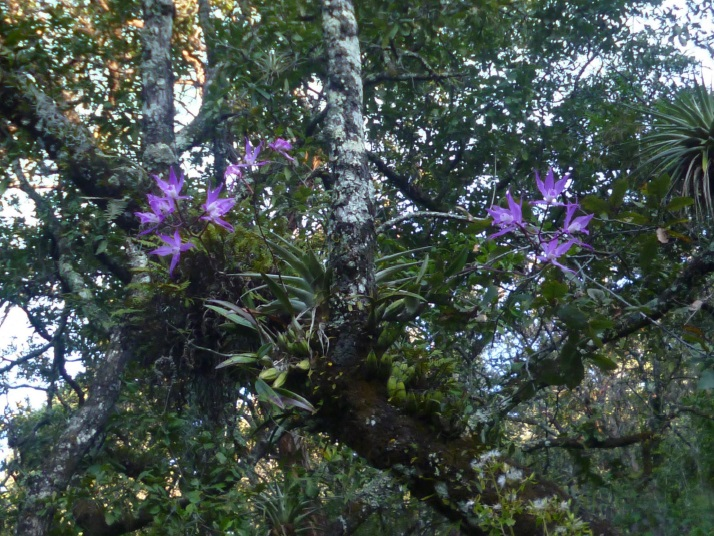
\includegraphics[keepaspectratio]{images/L_autum_epifita.jpg}}

}

\caption{\label{fig-laelia-epi}\emph{Laelia autumnalis} en hábitat
epífita, crédito: {[}autor{]}}

\end{figure}%

Al momento de localizar poblaciones en su hábitat natural, no basta con
conocer el tipo de vegetación donde se distribuye la especie de interés;
también es fundamental identificar su tipo de crecimiento. Este atributo
indica el sustrato o hábitat en el que las orquídeas se establecen y
desarrollan, pudiendo ser: terrestre, epífito o rupícola (también
denominado litófito) (Téllez \& Flores, 2007).

En términos generales:

\begin{itemize}
\tightlist
\item
  Las especies terrestres crecen directamente sobre el suelo.
\item
  Las epífitas se desarrollan sobre ramas y troncos de árboles.
\item
  Las rupícolas se establecen sobre rocas.
\end{itemize}

El tipo de crecimiento suele ser característico de ciertas subfamilias.
Por ejemplo, las especies de \emph{Cypripedioideae}, \emph{Orchidoideae}
y \emph{Spiranthoideae} son predominantemente terrestres, mientras que
las de \emph{Epidendroideae} se distinguen por su hábito mayormente
epífito (Cribb, 1999).

No obstante, como señala Rasmussen (Rasmussen, 1999), las especies no
están estrictamente limitadas a un único tipo de crecimiento. Existen
casos como \emph{Dipodium}, que puede ser tanto epífito como terrestre,
o géneros como \emph{Lepanthes} y \emph{Laelia}, que presentan hábitos
epífitos y rupícolas (ver Figura~\ref{fig-laelia-epi}).

\subsection{Identificación de las
orquídeas}\label{identificaciuxf3n-de-las-orquuxeddeas}

Durante la búsqueda de poblaciones en campo, resulta fundamental contar
con una capacitación adecuada que facilite la identificación precisa de
la especie de interés. Este proceso puede abordarse desde dos niveles:

\begin{itemize}
\tightlist
\item
  una aproximación inicial basada en la apariencia general, y
\item
  una determinación rigurosa mediante análisis botánico.
\end{itemize}

\subsubsection{Apariencia e identificación visual
preliminar}\label{apariencia-e-identificaciuxf3n-visual-preliminar}

La identificación visual, aunque menos precisa, permite reconocer de
manera general distintos géneros de orquídeas a partir de rasgos
morfológicos característicos. Estos atributos pueden incluir la forma y
disposición de las hojas, el tipo de pseudobulbo, la estructura floral y
el hábito de crecimiento. Con base en estas características, es posible
clasificar las orquídeas en grupos según su tipo de crecimiento:
terrestres, epífitas o rupícolas, lo que constituye un primer paso para
orientar la búsqueda y el muestreo en campo.

\begin{figure}

\centering{

\pandocbounded{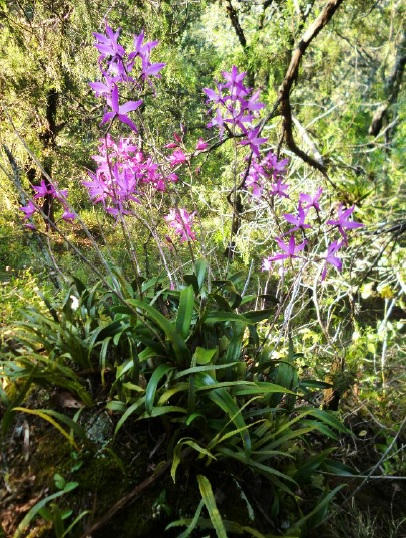
\includegraphics[keepaspectratio]{images/L_autum_rupicola.jpg}}

}

\caption{\label{fig-laelia-rupi}\emph{Laelia autumnalis} en su hábitat
rupícola, crédito: {[}autor{]}}

\end{figure}%

\begin{enumerate}
\def\labelenumi{\roman{enumi}.}
\tightlist
\item
  En las epífitas se reconocen al menos tres grupos de plantas:
\end{enumerate}

\begin{itemize}
\tightlist
\item
  con tallos engrosados y modificados (i.e.~pseudobulbos),
  e.g.~\emph{Laelia}, \emph{Oncidium}, \emph{Encyclia},
  \emph{Stanhopea}, \emph{Maxillaria} y \emph{Rhynchostele} (ver
  Figura~\ref{fig-laelia-rupi});
\item
  con tallos simples o delgados, e.g.~\emph{Epidendrum} y \emph{Dichea};
  y
\item
  con hojas engrosadas y tallos compactos o pseudobulbos poco visibles,
  e. g. \emph{Trichocentrum} (ver Figura~\ref{fig-trichocentrum-1} y
  Figura~\ref{fig-trichocentrum-2}).
\end{itemize}

\begin{enumerate}
\def\labelenumi{\roman{enumi}.}
\setcounter{enumi}{1}
\tightlist
\item
  En las terrestres se han identificado seis grupos:
\end{enumerate}

\begin{itemize}
\tightlist
\item
  con tallos y hojas alternas o en espiral, e. g. \emph{Cypripedium},
  \emph{Dichromanthus}, \emph{Habenaria} y \emph{Triphora};
\item
  con hojas solitarias o en pares, e.g.~\emph{Bletia},
  \emph{Schiedeella}, \emph{Malaxis} y \emph{Govenia};
\item
  con hojas en roseta, e.g.~\emph{Brachystele}, \emph{Deiregyne} y
  \emph{Sarcoglottis};
\item
  con hojas en abanico, e.g.~\emph{Paphiopedilum}, \emph{Phragmipedium};
\item
  sin hojas, e.g.~\emph{Rhizanthella}, \emph{Triphora}; y
\item
  con pseudobulbos, e.g.~\emph{Oeceoclades} y \emph{Cymbidium}.
\end{itemize}

\begin{enumerate}
\def\labelenumi{\roman{enumi}.}
\setcounter{enumi}{2}
\tightlist
\item
  En las rupícolas se han reconocido dos grupos:
\end{enumerate}

\begin{itemize}
\tightlist
\item
  con pseudobulbos e.g.~\emph{Cattleya}, \emph{Hoffmannseggella},
  \emph{Laelia} y \emph{Paphiopedilum}; y
\item
  sin pseudobulbo, e.g.~\emph{Lepanthes}.
\end{itemize}

\begin{figure}

\centering{

\pandocbounded{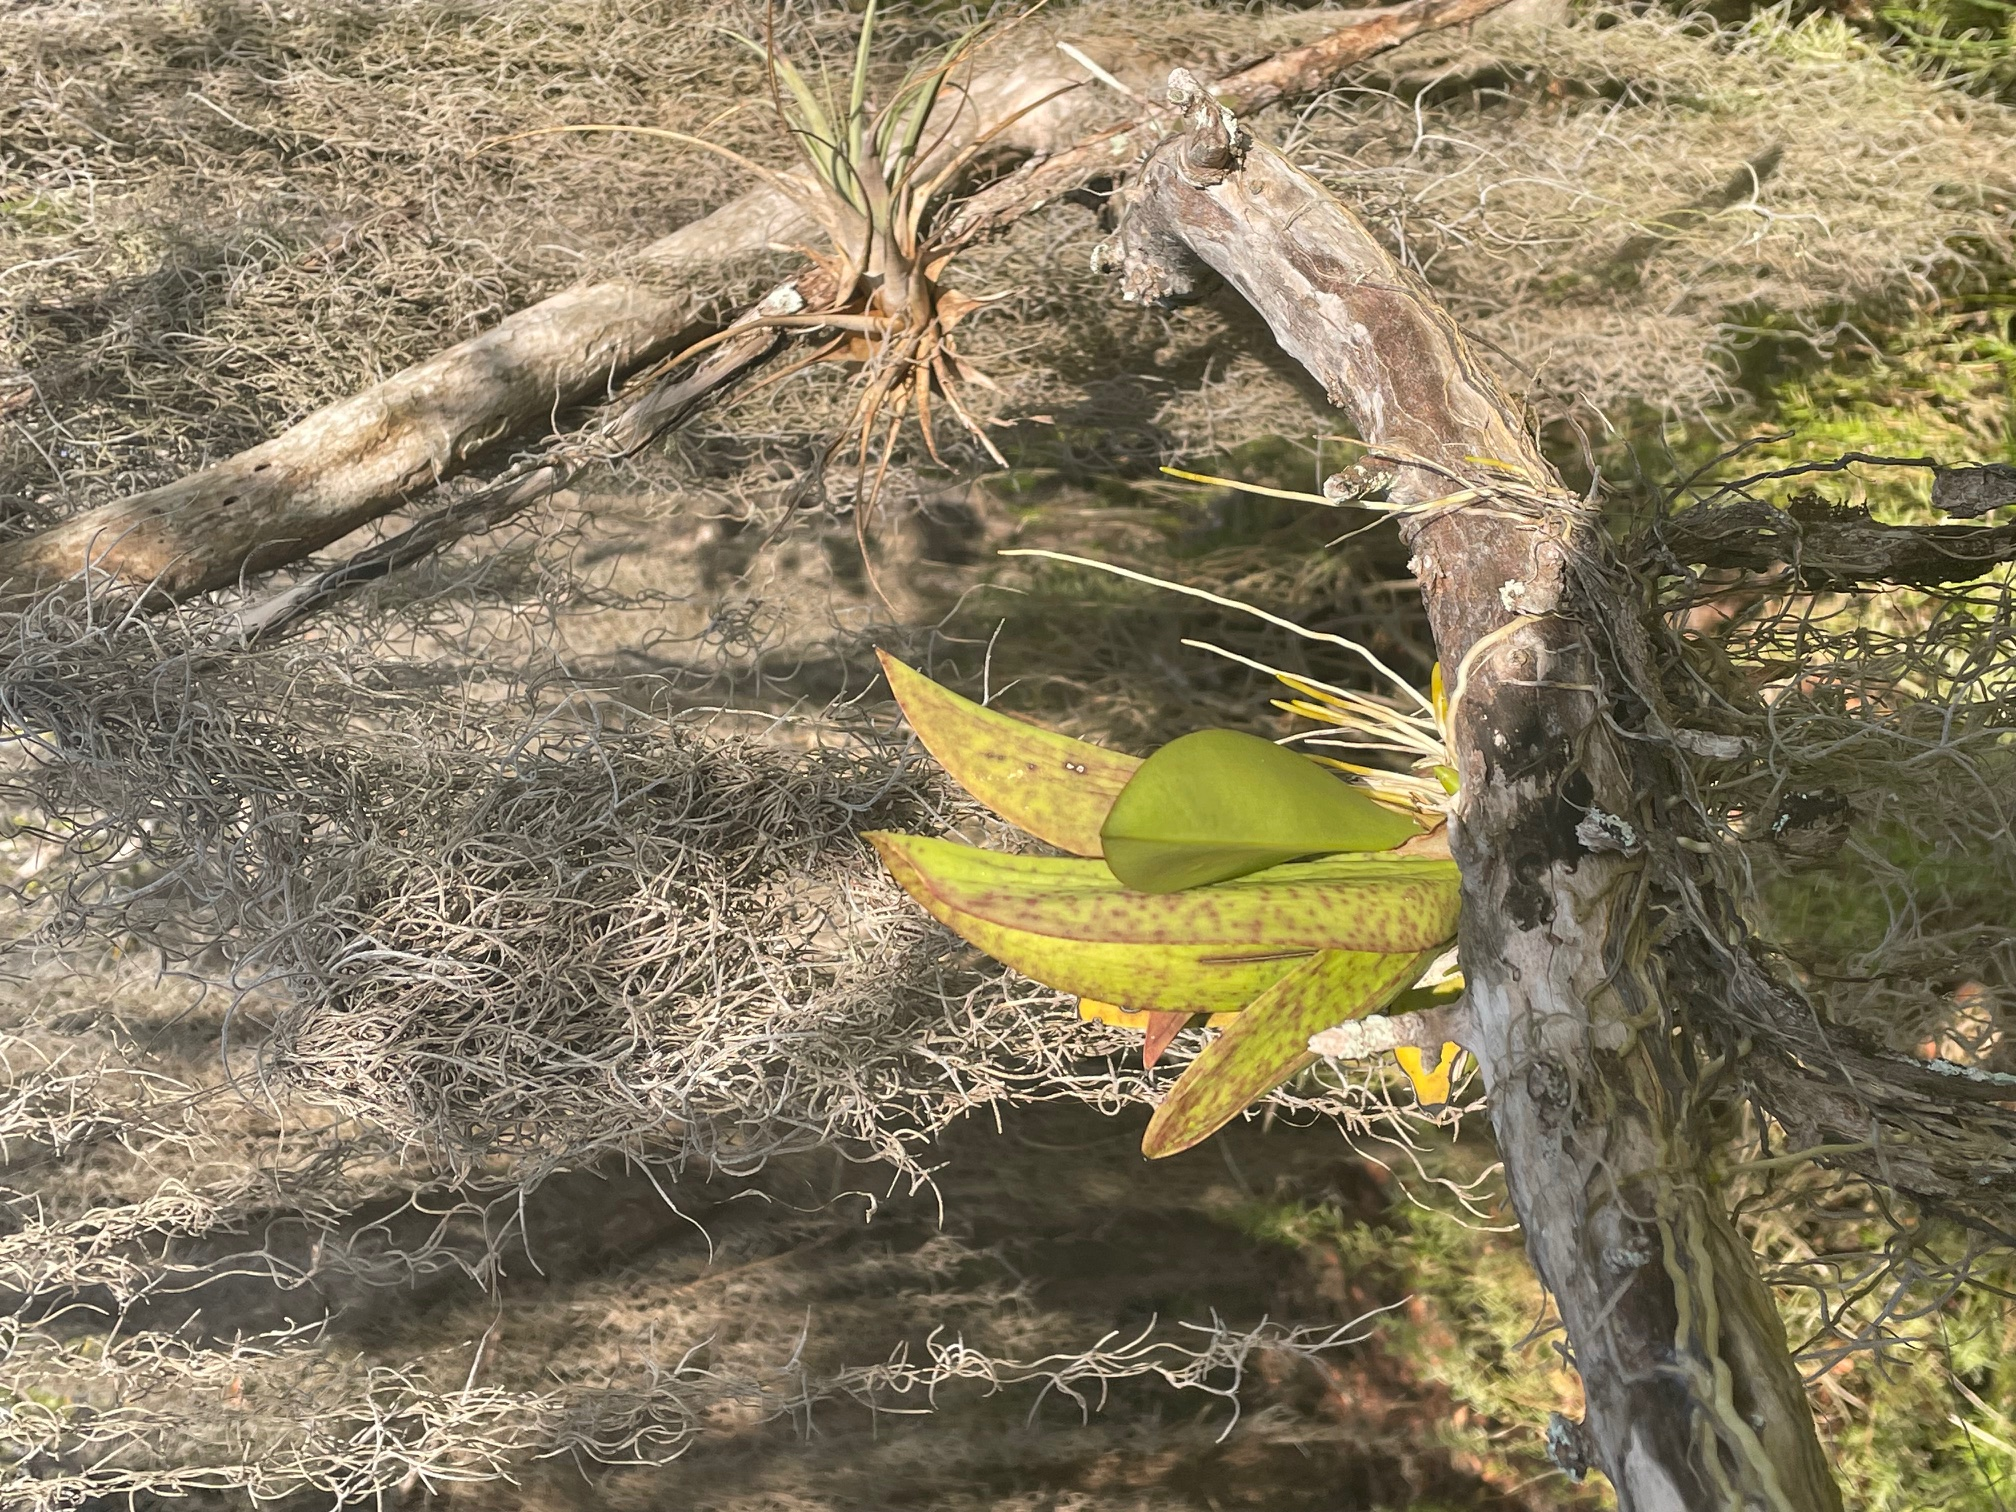
\includegraphics[keepaspectratio]{images/Trichocentrum_undulatum_9_Hong_Liu.jpeg}}

}

\caption{\label{fig-trichocentrum-1}\emph{Trichocentrum undulatum}.
Foto: Hong Liu}

\end{figure}%

\begin{figure}

\centering{

\pandocbounded{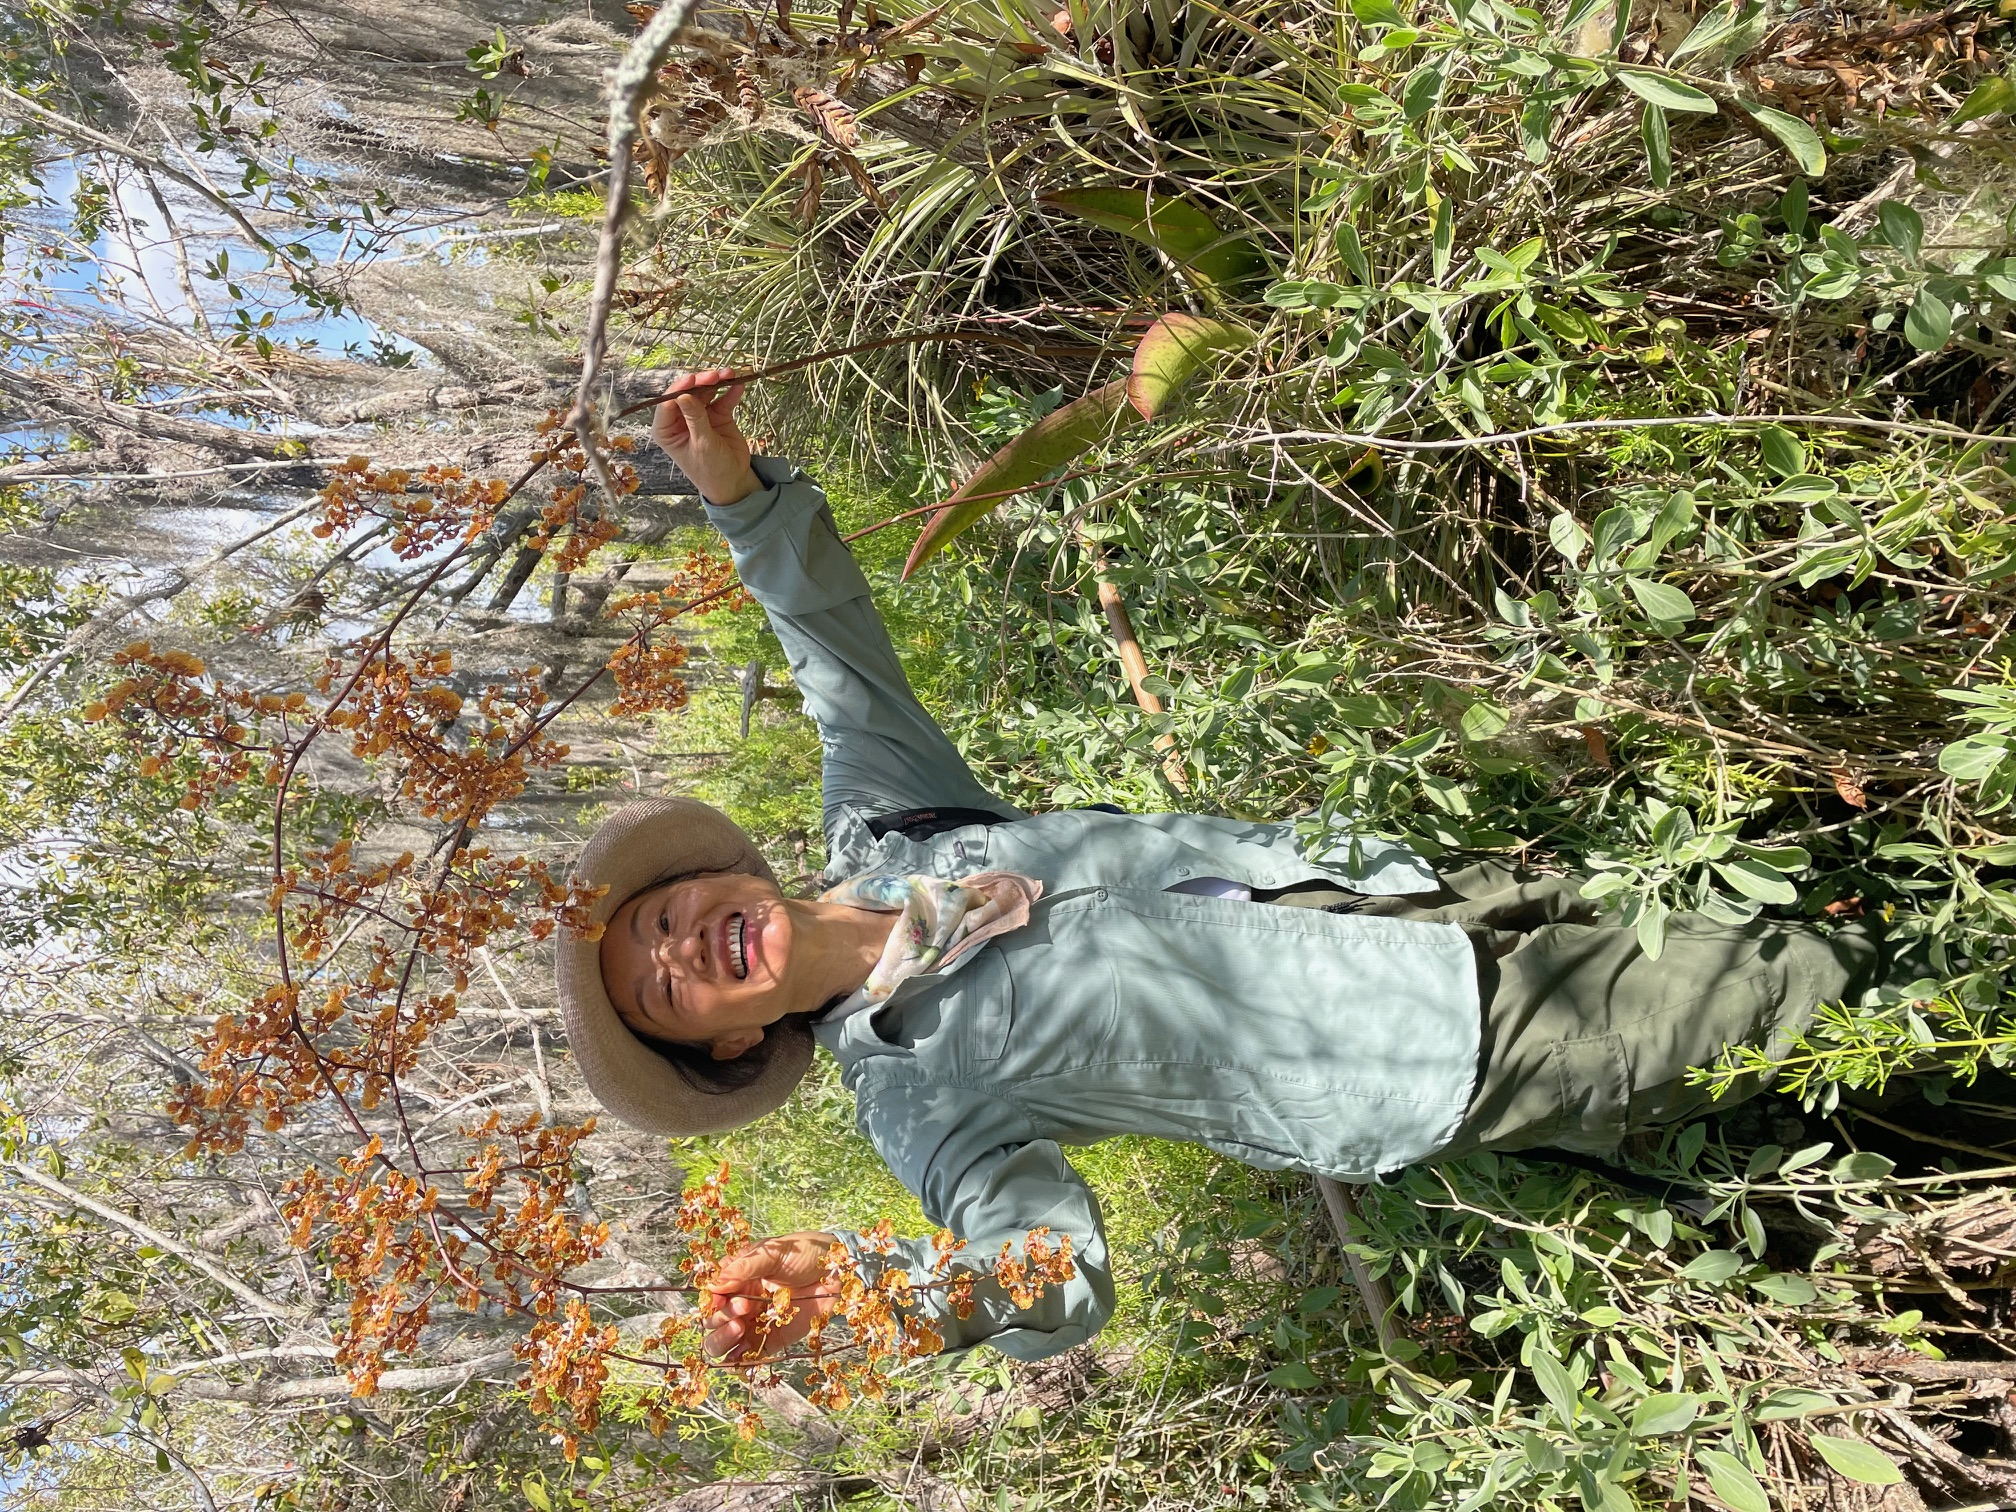
\includegraphics[keepaspectratio]{images/Trichocentrum_undulatum_1_Hong_Liu.jpg}}

}

\caption{\label{fig-trichocentrum-2}\emph{Trichocentrum undulatum}.
Foto: Hong Liu}

\end{figure}%

Cabe señalar que, si bien esta clasificación resulta útil para ofrecer
una visión general de la diversidad morfológica presente en las
orquídeas, su fundamento es principalmente descriptivo y visual, por lo
que carece de rigor desde una perspectiva botánica. Se trata de un
criterio cualitativo, basado en la apariencia externa de las plantas,
que facilita una identificación aproximada (\emph{grosso modo}), pero no
refleja necesariamente relaciones filogenéticas ni características
funcionales del grupo.

\subsubsection{Identificación botánica de la
especie}\label{identificaciuxf3n-botuxe1nica-de-la-especie}

Cuando no se dispone de estudios previos sobre la especie de interés, y
considerando la gran diversidad de la familia \emph{Orchidaceae}, es
fundamental garantizar la identificación taxonómica. Para ello, se
recomienda contar con el apoyo de un especialista en la familia. Este
proceso requiere disponer de una muestra fértil, ya sea fresca o
herborizada, que incluya estructuras diagnósticas como hojas, tallos o
pseudobulbos, flores y/o frutos, en estado fresco o seco.

El acompañamiento de un experto resulta aún más necesario cuando dos o
más especies del mismo género coexisten en el mismo hábitat, ya que
pueden presentar características morfológicas y florales muy similares,
lo que incrementa el riesgo de confusión. Por ejemplo, en el género
\emph{Lepanthes} es particularmente difícil diferenciar individuos
recién germinados (Tremblay, comunicación personal, fecha), debido a su
gran similitud morfológica. En estas primeras etapas, la semejanza puede
ser tan marcada que incluso especies de familias distintas, como
\emph{Bromeliaceae} y \emph{Orchidaceae}, podrían confundirse por
personas sin experiencia. En tales casos, la intervención de un botánico
especializado es esencial para evitar errores en la identificación y
garantizar la validez de los datos.

\begin{center}\rule{0.5\linewidth}{0.5pt}\end{center}

\subsection{Etapas o estados de desarrollo en
orquídeas}\label{sec-etapas-orquideas}

Aunque las poblaciones están conformadas por individuos de la misma
especie, en los estudios demográficos se reconoce que su contribución a
la abundancia poblacional varía según la etapa o estado de desarrollo en
que se encuentren (véase el \hyperref[Ciclo_Vida]{Capítulo de Ciclo de
Vida}). Al igual que en los seres humanos, donde se distinguen fases
como recién nacidos, infantes, adolescentes y adultos, las plantas
atraviesan diferentes etapas a lo largo de su vida, tales como semillas,
plántulas, juveniles, adultos de tamaño pequeño y adultos de gran
tamaño, entre otras.

Cada etapa debe asociarse a características biológicas y morfológicas
que permitan su identificación en campo. Por ejemplo, la presencia de
flores, frutos o varas florales (escapos) frescos o secos se vincula con
la fase adulta en las orquídeas, lo que facilita diferenciar a los
individuos reproductivos del resto de la población. Aunque la fase
adulta es la más familiar para los orquidófilos, las poblaciones también
incluyen individuos no reproductivos: juveniles (similares a los adultos
pero sin estructuras reproductivas), plántulas (individuos pequeños
recién establecidos) y semillas, responsables de la dispersión y
perpetuación de la especie. Esta clasificación constituye la estructura
poblacional (Silvertown \& Charlesworth, 2009).

La delimitación de estas etapas puede requerir criterios específicos. Un
ejemplo es el trabajo de Tremblay y colaboradores (Tremblay \&
Hutchings, 2003) con \emph{Lepanthes}, donde se diferenciaron plántulas
y juveniles mediante la presencia de una vaina lepanthiforme
(\emph{lepanthiform sheath}) en al menos uno de los pecíolos. Los
individuos no reproductivos sin esta estructura fueron considerados
plántulas. Para distinguir juveniles de adultos, además de las vainas en
pecíolos, se consideró la presencia de inflorescencias secas o activas,
estas últimas en floración, con escapos en desarrollo (indicando
floración potencial) o secos (evidencia de floración previa), tal como
se ilustra en la Figura~\ref{fig-lep-rupestris}.

\begin{figure}

\centering{

\pandocbounded{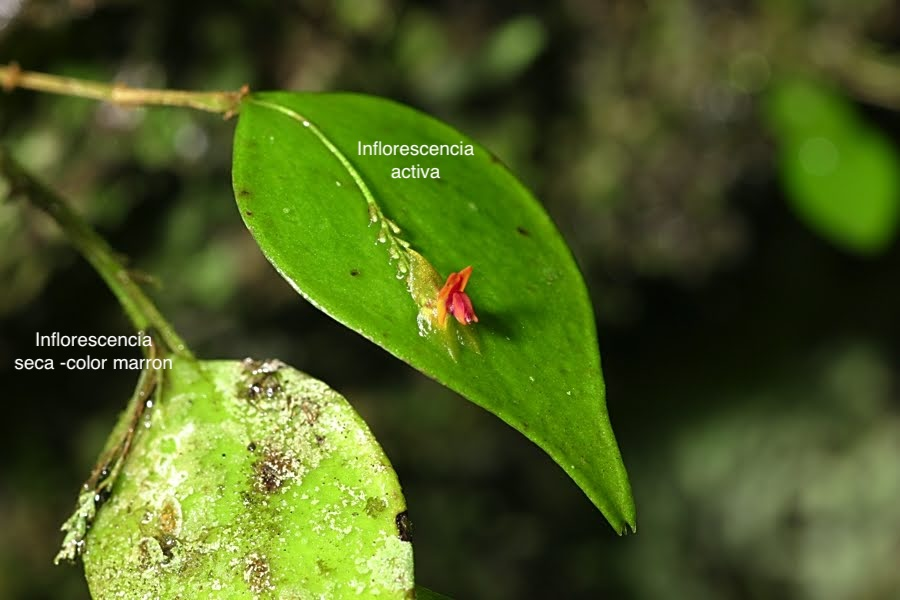
\includegraphics[keepaspectratio]{images/lepanthes_rupestris.jpeg}}

}

\caption{\label{fig-lep-rupestris}\emph{Lepanthes rupestris} con
inflorescencias seca y activa. Foto: Tremblay}

\end{figure}%

En las plantas, la definición de las etapas del ciclo de vida de una
población puede incluir un número mayor o menor que las cuatro
categorías comúnmente utilizadas (semillas, plántulas, juveniles y
adultos). Esta variación se debe a que las categorías pueden
subdividirse o agruparse, como se discutirá en la sección
\hyperref[sec-ejemplos-categorizacion]{Ejemplos de categorización en
especies de estudio}.

Independientemente del número de etapas o estados definidos para una
población, es fundamental contar con un sistema de clasificación claro y
sencillo, basado en características distintivas y únicas de cada etapa.
Este principio garantiza la coherencia en la recolección de datos y la
interpretación de los procesos demográficos, evitando ambigüedades que
puedan comprometer la validez del análisis.

\begin{center}\rule{0.5\linewidth}{0.5pt}\end{center}

\section{Ontogenia y estrategias de
crecimiento}\label{ontogenia-y-estrategias-de-crecimiento}

Para definir las etapas de desarrollo, es fundamental comprender cómo
ocurre el crecimiento a nivel individual en las orquídeas. Este proceso
permite inferir el incremento en volumen o tamaño de cada planta,
resultado tanto del crecimiento vegetativo como del crecimiento
reproductivo (Harper, 1977); es decir:

\begin{itemize}
\tightlist
\item
  El crecimiento vegetativo se refiere a la formación de nuevas
  estructuras no reproductivas que conforman el cuerpo de la planta,
  tales como hojas, tallos, raíces, pseudobulbos y ramas.
\item
  El crecimiento reproductivo, por su parte, implica la producción de
  flores, inflorescencias, frutos y semillas.
\end{itemize}

En las orquídeas, ambos tipos de crecimiento se originan a partir de la
activación de una yema de reiteración, mecanismo que permite la
generación de nuevas estructuras y la continuidad del ciclo vital
(Dressler, 1993).

\begin{figure}

\centering{

\pandocbounded{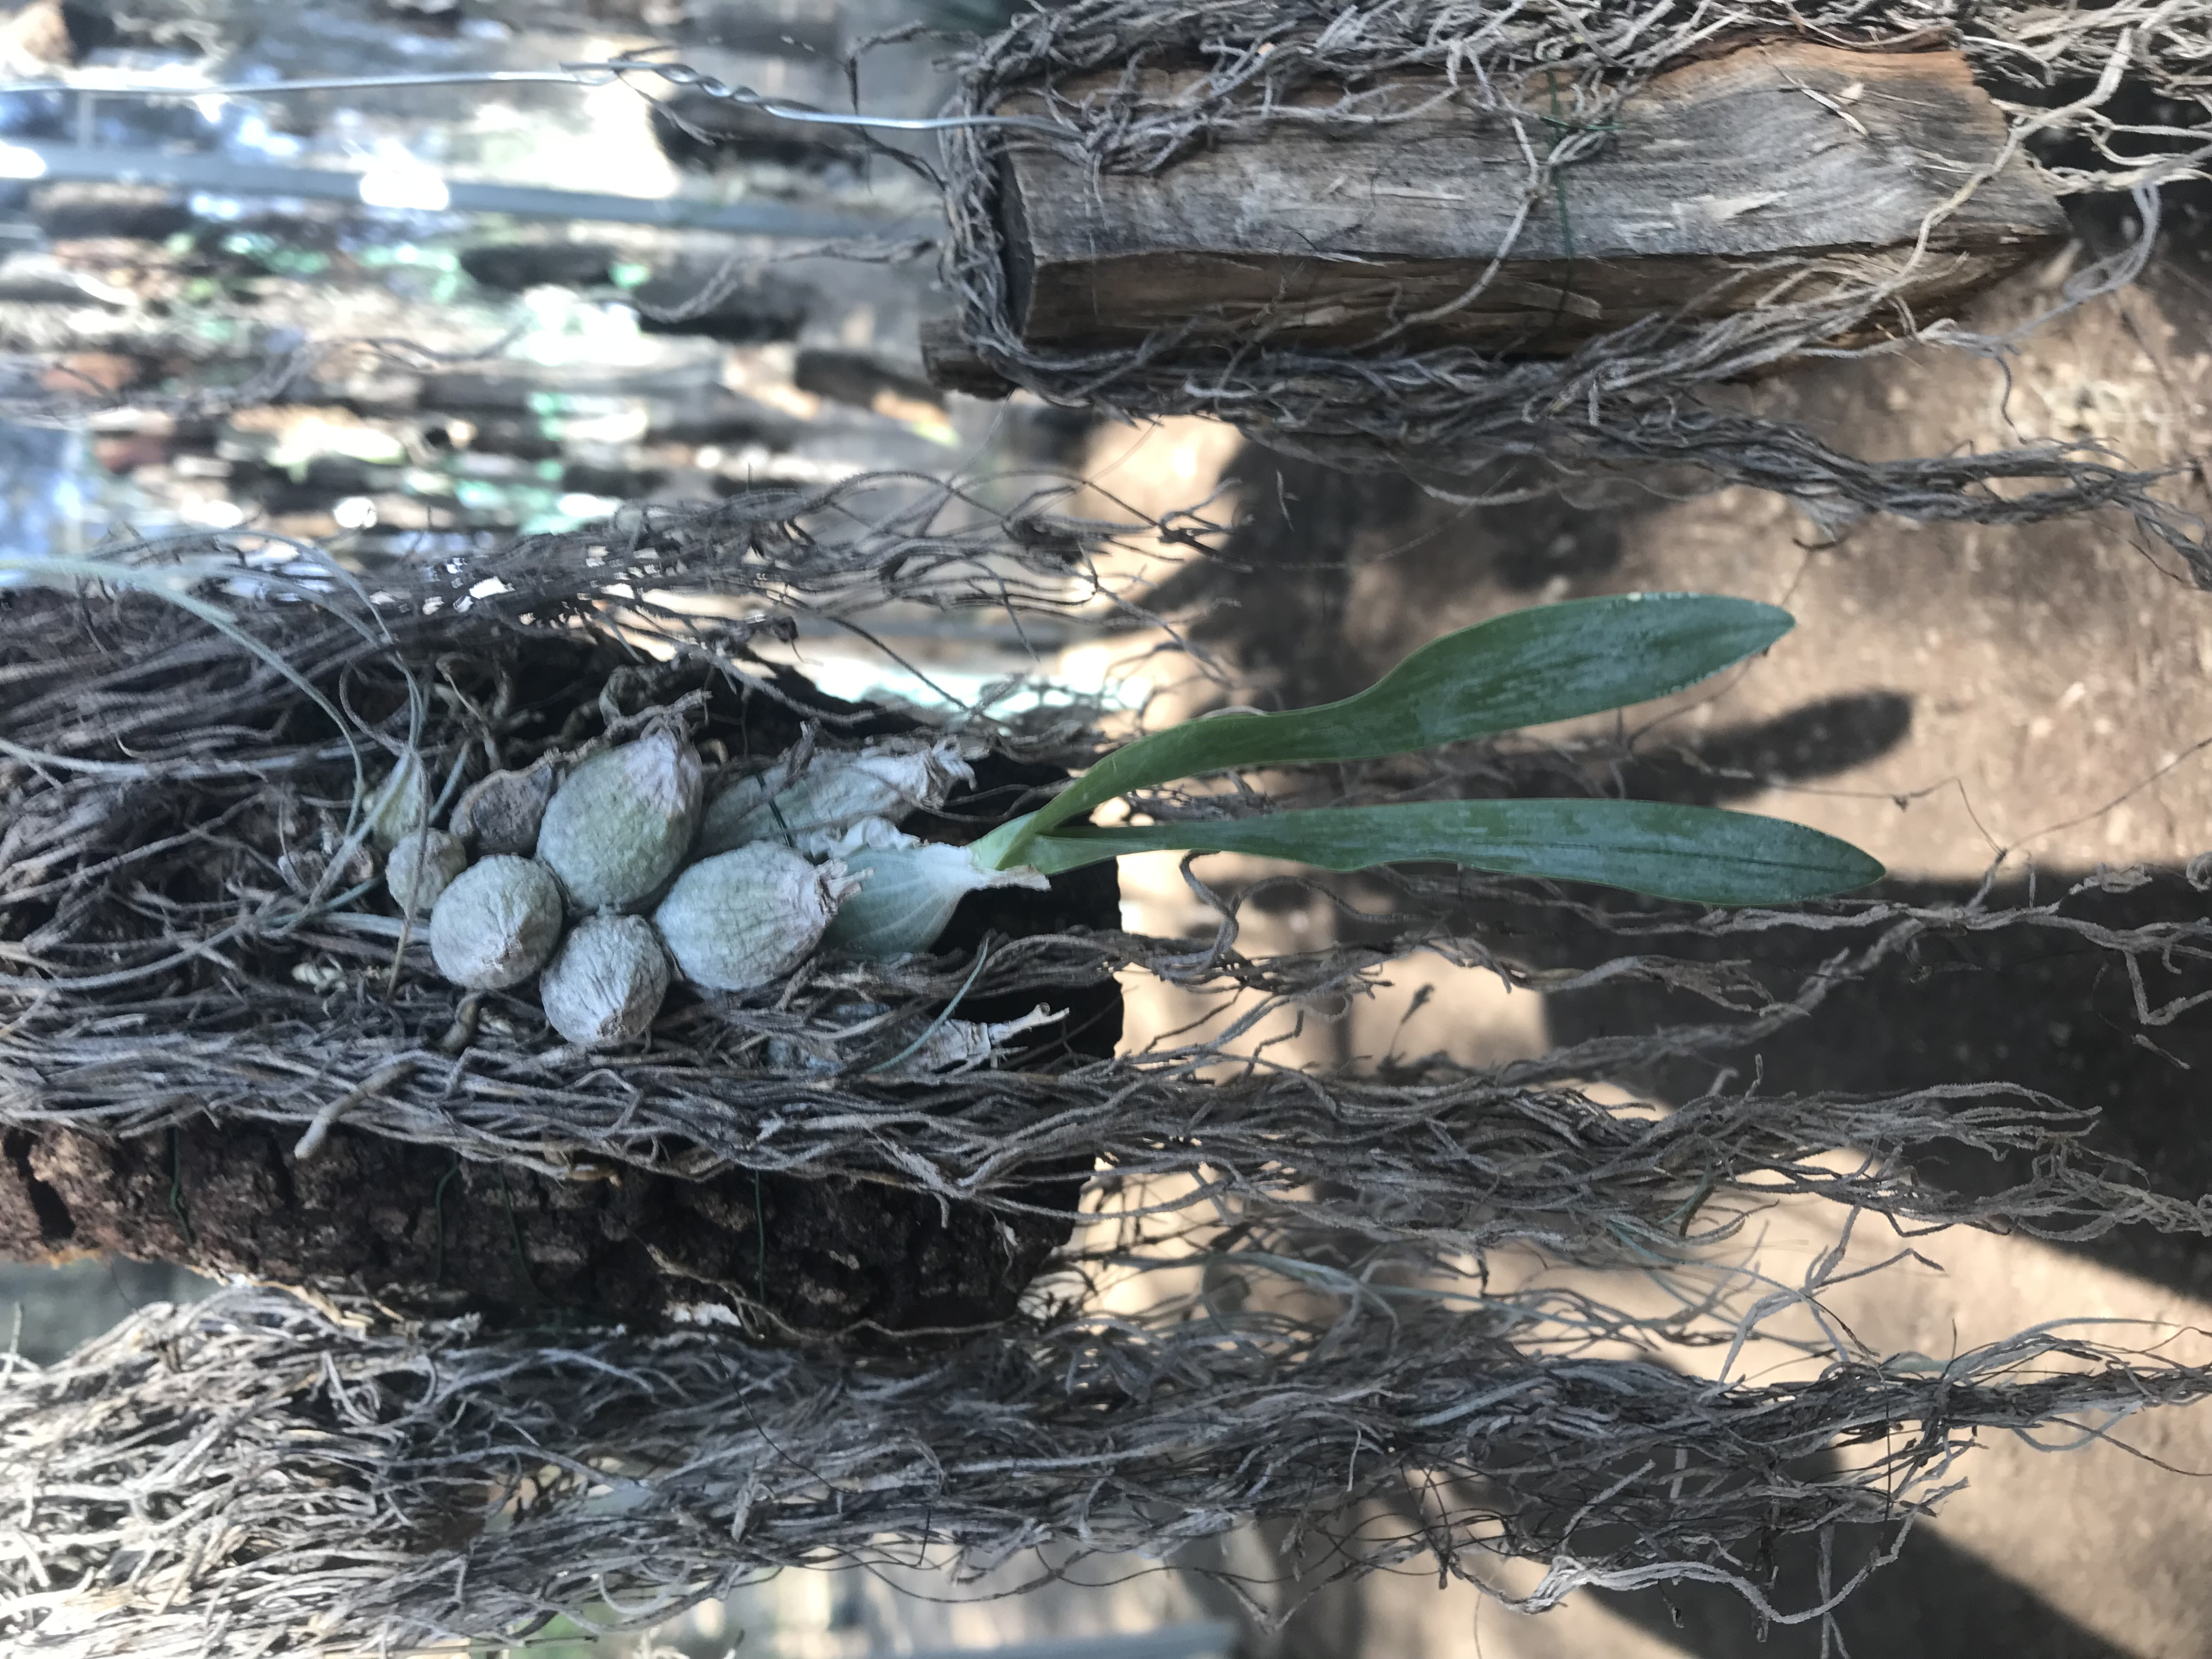
\includegraphics[keepaspectratio]{images/Pk_modulo.jpeg}}

}

\caption{\label{fig-pk-modulo}\emph{Prosthechea karwinskii}. Foto:
Mariana Hernández-Apolinar}

\end{figure}%

Como ocurre en todas las plantas (Harper, 1977), las estructuras
vegetativas y reproductivas generadas a partir de las yemas de
reiteración se organizan en unidades repetitivas denominadas módulos,
que en conjunto conforman el cuerpo de la orquídea. Este patrón define
un hábito de crecimiento modular (Holttum, 1995).

Por ejemplo:

\begin{itemize}
\tightlist
\item
  En \emph{Prosthechea karwinskii} (ver Figura~\ref{fig-pk-modulo}), el
  módulo incluye una yema de reiteración, pseudobulbo, hojas, rizoma,
  raíces, flores y frutos.
\item
  En \emph{Cypripedium irapeanum} (ver Figura~\ref{fig-ci-modulo}), el
  módulo comprende una yema de reiteración, rizoma, raíces, tallo,
  hojas, flores y frutos.
\end{itemize}

Para un análisis detallado de la morfología y del impacto del
crecimiento modular en los procesos evolutivos, véase el libro de Carlos
Herrera \emph{Multiplicity in Unity} (Herrera, 2009).

El hábito de crecimiento ---la forma o disposición final de la planta
(erecta, rastrera o colgante)--- también está determinado por la
posición de las yemas de reiteración. Se reconocen dos tipos
principales:

\begin{itemize}
\tightlist
\item
  Monopodial, donde la yema es apical; y
\item
  Simpodial, donde la yema es axilar (Dressler, 1993; Hágsater, 2005).
\end{itemize}

\begin{figure}

\centering{

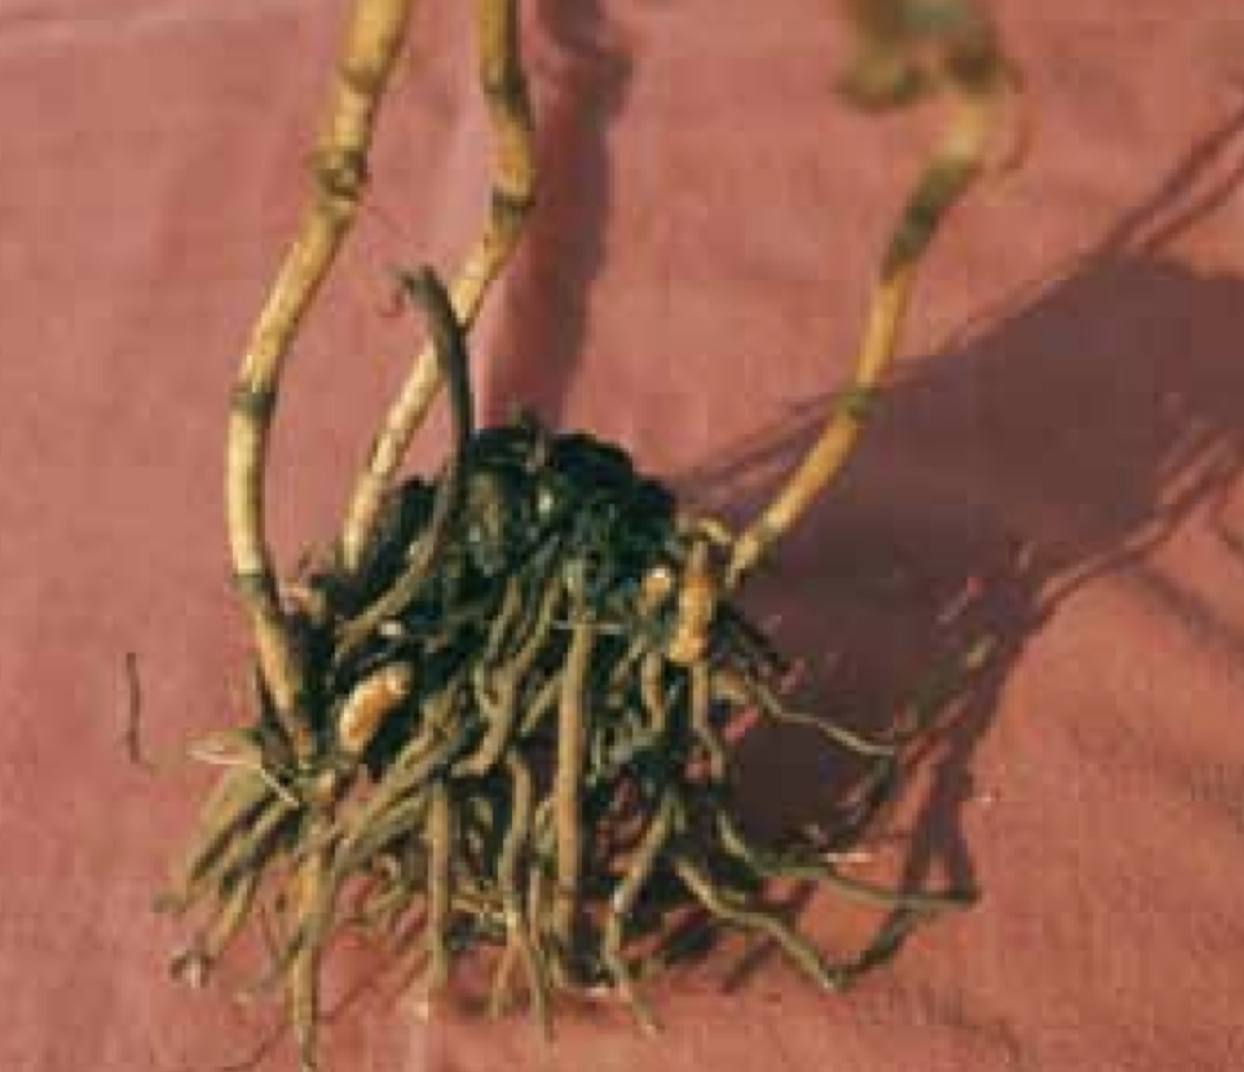
\includegraphics[width=0.5\linewidth,height=\textheight,keepaspectratio]{images/Ci_modulo.png}

}

\caption{\label{fig-ci-modulo}\emph{Cypripedium irapeanum}. Foto:
Claudia C. Gutiérrez-Paredes}

\end{figure}%

El hábito monopodial se caracteriza por la presencia de un eje
vegetativo principal o tallo único vertical (módulo), originado por la
reiteración consecutiva de la yema apical. En este patrón, las flores o
inflorescencias se desarrollan de manera lateral (Dressler, 1993). Este
tipo de crecimiento se observa en géneros como \emph{Campylocentrum},
\emph{Dendrophylax}, \emph{Dichea}, \emph{Renanthera}, \emph{Vanilla} y
\emph{Vanda} (ver Figura~\ref{fig-vanilla}).

Por otro lado, el hábito simpodial se define por el crecimiento mediante
brotes consecutivos (módulos), que pueden estar agrupados o separados y
conectados por un rizoma. Estos brotes se originan a partir de una yema
axilar, ubicada basal, lateral o apicalmente en el brote anterior. En
este patrón, las flores o inflorescencias en plantas adultas son
apicales o laterales, como ocurre en géneros tales como
\emph{Cypripedium}, \emph{Laelia} y \emph{Prosthechea} (ver
Figura~\ref{fig-laelia-speciosa}).

\begin{figure}

\centering{

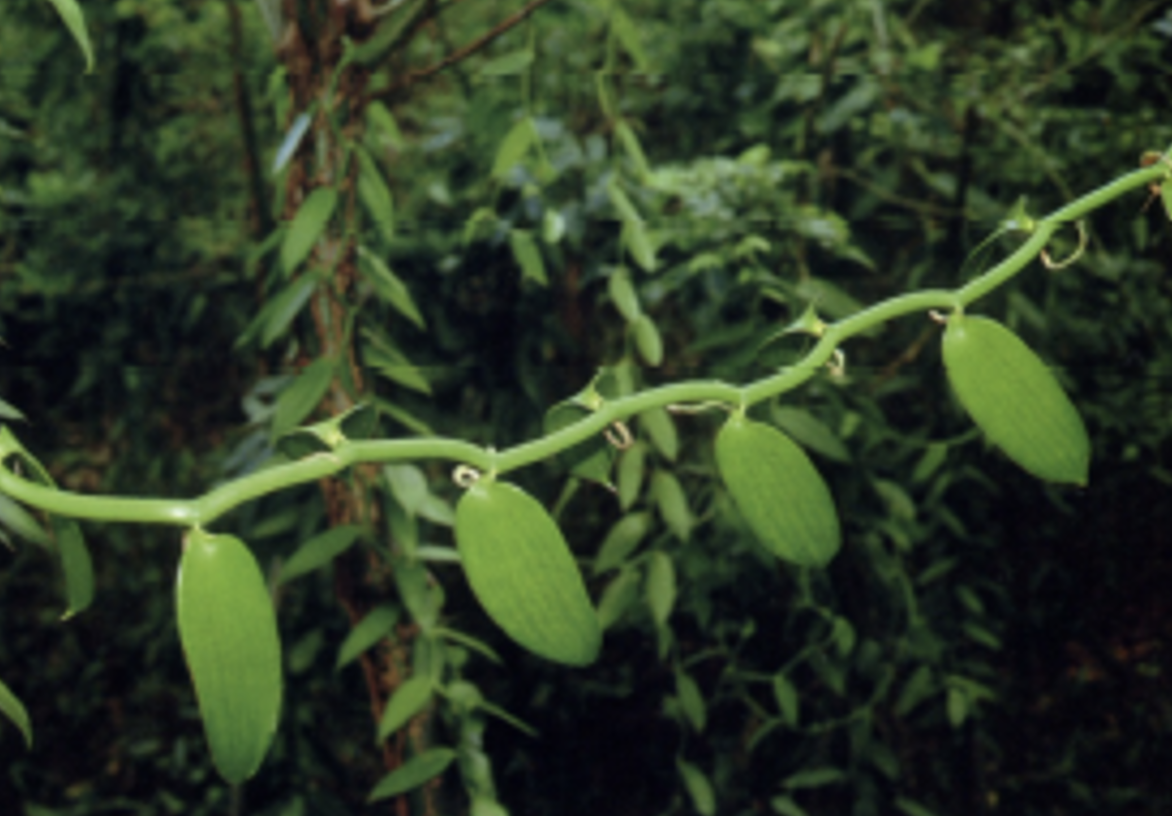
\includegraphics[width=0.5\linewidth,height=\textheight,keepaspectratio]{images/V_planifolia_monopo.png}

}

\caption{\label{fig-vanilla}\emph{Vanilla planifolia}. Foto: Mark
Blackman}

\end{figure}%

\begin{figure}

\centering{

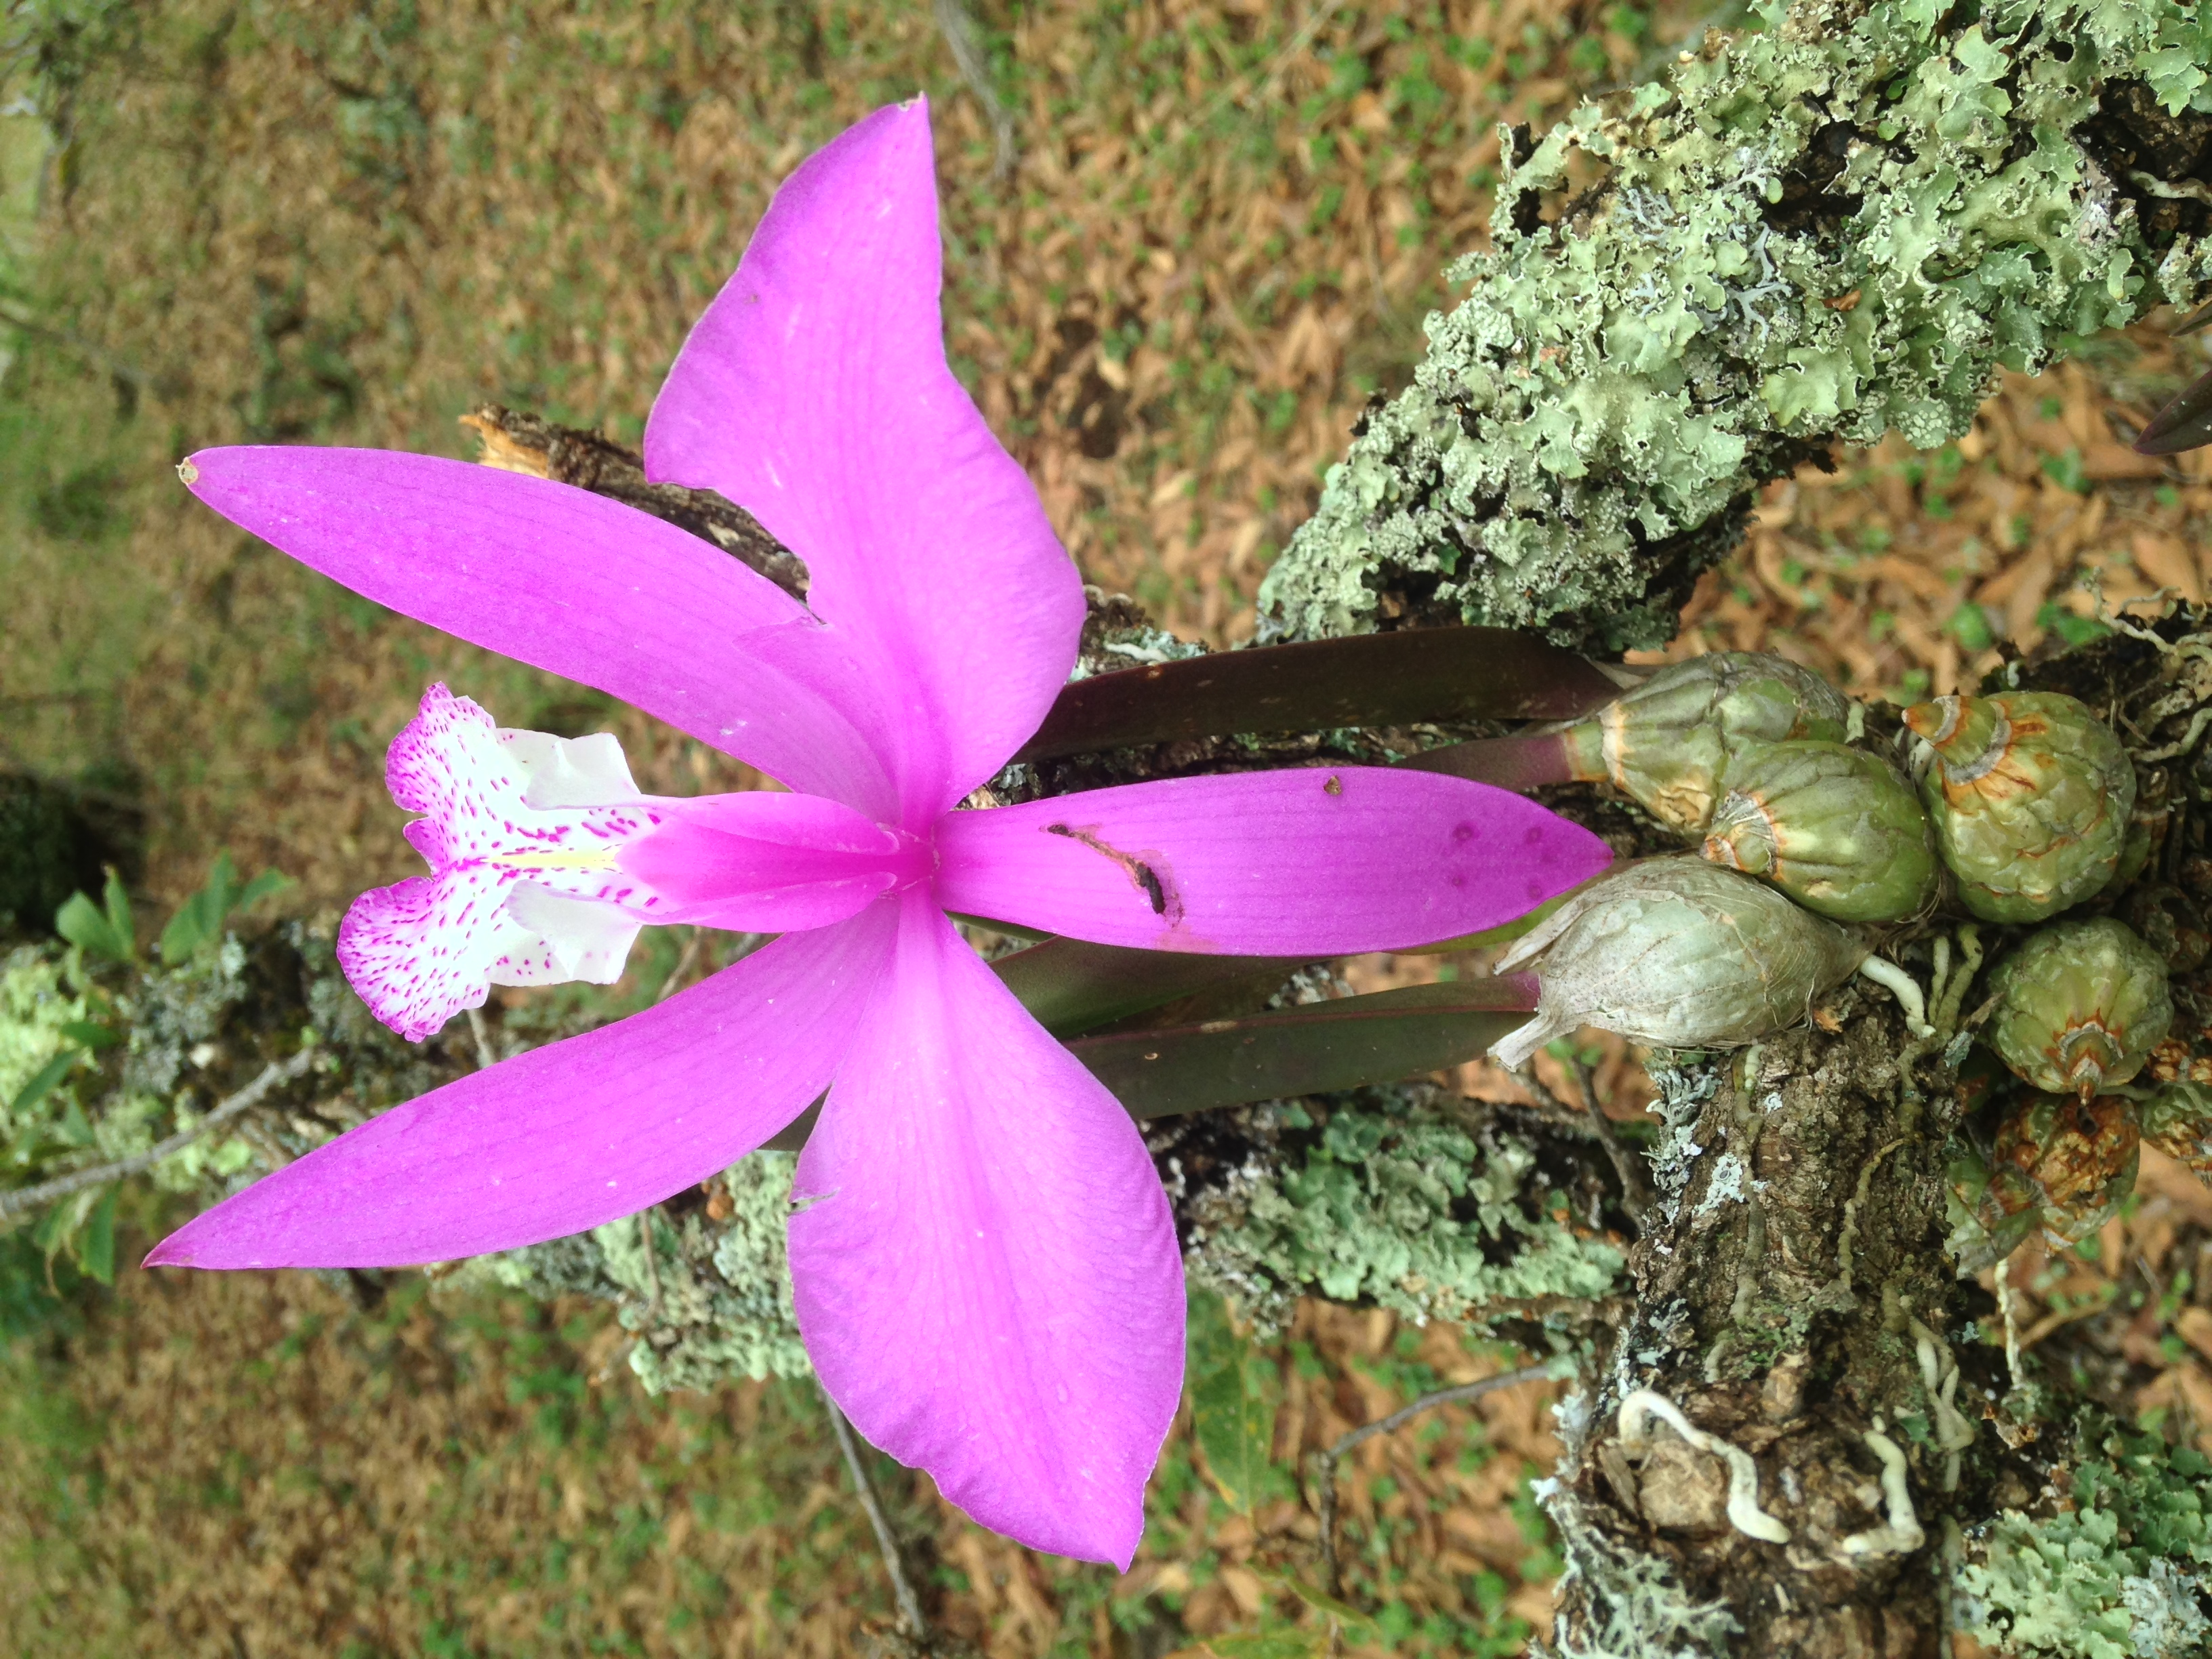
\includegraphics[width=0.5\linewidth,height=\textheight,keepaspectratio]{images/Ls_simpodio.jpg}

}

\caption{\label{fig-laelia-speciosa}\emph{Laelia speciosa}. Foto: Leonel
López-Toledo}

\end{figure}%

Según Rasmussen (Rasmussen, 1986), las orquídeas presentan más de una
yema de regeneración, clasificadas en dos tipos según su actividad:
yemas de renuevo y yemas de reserva; o sea:

\begin{itemize}
\tightlist
\item
  Las yemas de renuevo se activan regularmente y aseguran la continuidad
  del crecimiento de la planta en cada temporada.
\item
  Las yemas de reserva, en cambio, permanecen inactivas y se activan de
  manera eventual; por ejemplo, cuando la yema de renuevo es eliminada
  por ramoneo de herbívoros (Emeterio-Lara et~al., 2016), o cuando las
  condiciones ambientales son favorables para sostener el desarrollo de
  más de un módulo.
\end{itemize}

En este último caso, la activación de yemas de reserva genera nuevas
líneas o frentes de crecimiento, lo que incrementa el tamaño de la
planta. Este fenómeno ha sido documentado en especies como
\emph{Cypripedium irapeanum} y \emph{Govenia lagenophora}
(Hernández-Apolinar et~al., 2012; Martı́nez-Villegas et~al., 2024).

\begin{center}\rule{0.5\linewidth}{0.5pt}\end{center}

\section{Consideraciones durante la colecta de
datos}\label{consideraciones-durante-la-colecta-de-datos}

A continuación se describen los métodos y técnicas más comunes
utilizados para acceder a las poblaciones de orquídeas en el campo.

\subsection{Métodos y técnicas de
muestreo}\label{muxe9todos-y-tuxe9cnicas-de-muestreo}

Las orquídeas epífitas y rupícolas se distribuyen a diferentes alturas
en árboles y acantilados, lo que implica retos logísticos y de seguridad
en la colecta de información. Las técnicas empleadas pueden ser tan
rudimentarias como el uso de escaleras, hasta tan especializadas como
equipos de ascenso utilizados en alpinismo. Cabe señalar que estas
mismas técnicas han sido empleadas para la extracción ilegal de
orquídeas (Drugs \& Crime, 2024). A continuación se describen tres
técnicas:

\begin{enumerate}
\def\labelenumi{\arabic{enumi}.}
\item
  \textbf{Uso de escaleras.} Esta técnica es práctica cuando las
  orquídeas se encuentran en zonas bajas de acantilados o en forófitos
  como arbustos y árboles de porte bajo a medio (Hernández-Apolinar,
  1992). Su principal desventaja es la dificultad de transportar el
  equipo hasta el sitio de muestreo.
\item
  \textbf{Técnica de rapel.} Resulta útil y segura cuando las orquídeas
  se localizan a gran altura en acantilados. Consiste en descender
  mediante cuerdas hasta alcanzar los individuos a muestrear. Es
  fundamental contar con experiencia o apoyo de personal especializado
  (Larson \& Batson, 1978). Ver Figura~\ref{fig-ascenso-laelia}.
\item
  \textbf{Ascenso con cuerda única.} Esta técnica es considerada segura
  (Jepson, 2000) para acceder a orquídeas epífitas en árboles de porte
  medio y alto con troncos y ramas robustas. Sin embargo, presenta
  limitaciones para alcanzar ramas delgadas en estratos superiores. Al
  igual que en el rapel, se recomienda la asistencia de expertos para
  evitar riesgos. Ver Figura~\ref{fig-ascenso-pk}.
\end{enumerate}

\begin{figure}

\centering{

\pandocbounded{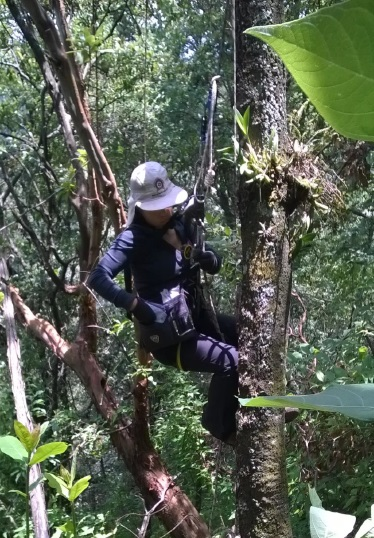
\includegraphics[keepaspectratio]{images/Aucencia_ascenso.jpg}}

}

\caption{\label{fig-ascenso-laelia}Muestreo de orquídeas epífitas con
ascenso de una sola cuerda: a) \emph{Laelia autumnalis}. Foto: Aucencia
Emeterio-Lara}

\end{figure}%

\begin{figure}

\centering{

\pandocbounded{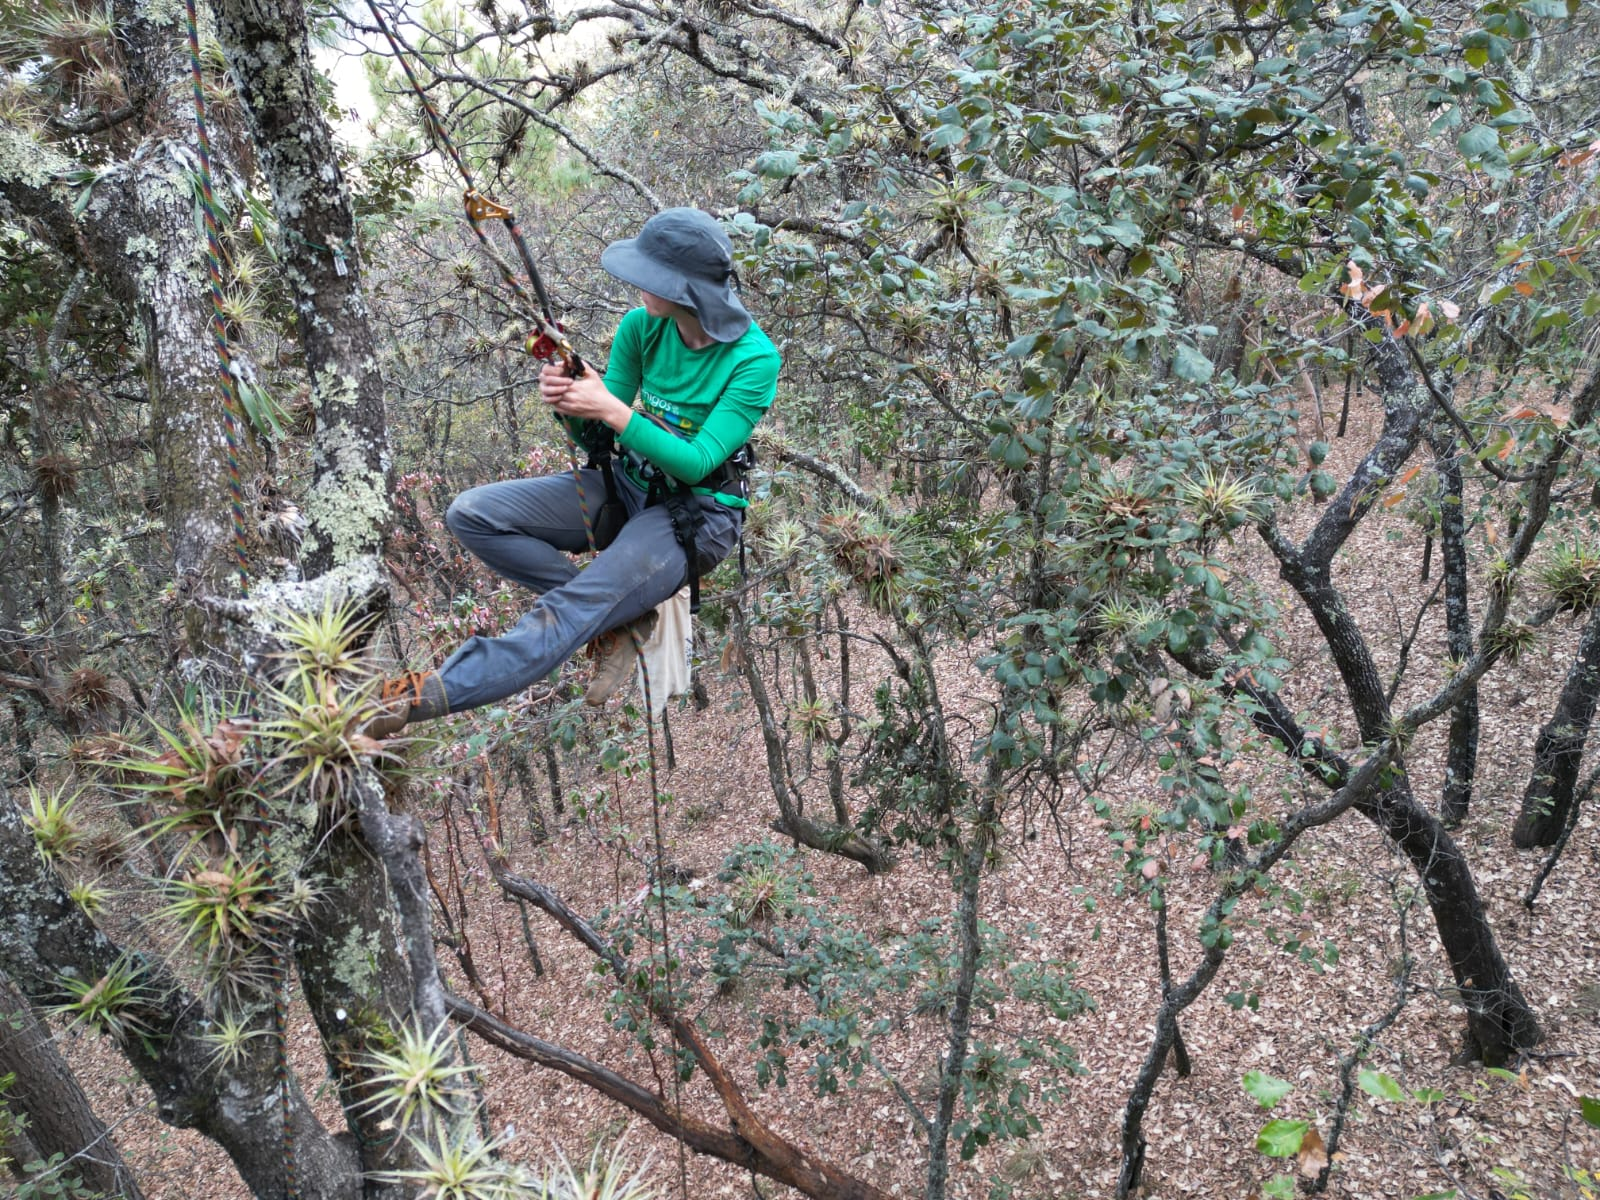
\includegraphics[keepaspectratio]{images/Ascenso_Pk.jpg}}

}

\caption{\label{fig-ascenso-pk}Muestreo de orquídeas epífitas con
ascenso de una sola cuerda: \emph{Prosthechea karwinskii}. Foto: Alonso
Argüero}

\end{figure}%

Debido a que la copa de los árboles no es un ambiente homogéneo
(Johansson, 1974; Catling, 1986), durante el ascenso se debe reportar la
zona en que se encuentran las plantas marcadas. Esta información permite
suponer las condiciones microclimáticas preferentes para la especie. De
acuerdo con Johansson (Johansson, 1974) y Catling (Catling, 1986), en un
árbol hospedero existen seis zonas o estratos, en las cuales es distinta
la predominancia de epífitas vasculares y no vasculares, tal como se
destaca en la Tabla~\ref{tbl-zonas-arbol}. Podemos apreciar
particularmente que en los estratos medios II, III, IV se registra la
mayor concentración de orquídeas (Mondragón, Maldonado \&
Aguilar-Santelises, 2007), mientras que la Zona VI está asociada a las
ramas más externas y delgadas del árbol, las cuales sobrepasan el límite
de la zona V, en donde raramente se encuentran algunas orquídeas.

\begin{center}\rule{0.5\linewidth}{0.5pt}\end{center}

\section{Zona de distribución de orquídeas en
árboles}\label{zona-de-distribuciuxf3n-de-orquuxeddeas-en-uxe1rboles}

La Figura~\ref{fig-zonificacion} muestra las zonas de vida de epífitas
basado en Johansson (1974) y Catling (1986) (ver también
Tabla~\ref{tbl-zonas-arbol}).

\begin{figure}

\centering{

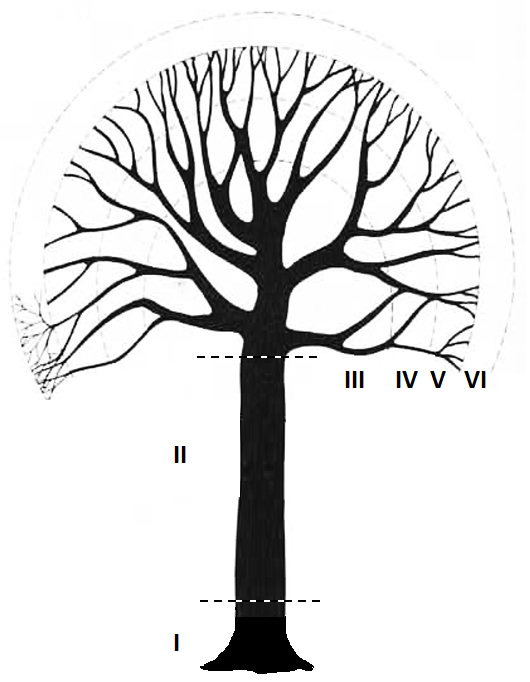
\includegraphics[width=0.4\linewidth,height=\textheight,keepaspectratio]{images/Cattling_y_Johannson.png}

}

\caption{\label{fig-zonificacion}Zonificación de árboles hospedero,
basada en los modelos Catling (1986) y Johansson (1974). Dibujo por A.
Emeterio Lara}

\end{figure}%

\begin{center}\rule{0.5\linewidth}{0.5pt}\end{center}

Las zonas se pueden describir de la siguiente manera:

\global\setlength{\Oldarrayrulewidth}{\arrayrulewidth}

\global\setlength{\Oldtabcolsep}{\tabcolsep}

\setlength{\tabcolsep}{2pt}

\renewcommand*{\arraystretch}{1.5}



\providecommand{\ascline}[3]{\noalign{\global\arrayrulewidth #1}\arrayrulecolor[HTML]{#2}\cline{#3}}

\begin{longtable}[c]{cc}

\caption{\label{tbl-zonas-arbol}Zonificación de árbol hospedero.}

\tabularnewline

\ascline{1.5pt}{666666}{1-2}

\multicolumn{1}{>{}l}{\textcolor[HTML]{000000}{\fontsize{11}{11}\selectfont{Zona}}} & \multicolumn{1}{>{}l}{\textcolor[HTML]{000000}{\fontsize{11}{11}\selectfont{Descripción}}} \\

\ascline{1.5pt}{666666}{1-2}\endfirsthead 

\ascline{1.5pt}{666666}{1-2}

\multicolumn{1}{>{}l}{\textcolor[HTML]{000000}{\fontsize{11}{11}\selectfont{Zona}}} & \multicolumn{1}{>{}l}{\textcolor[HTML]{000000}{\fontsize{11}{11}\selectfont{Descripción}}} \\

\ascline{1.5pt}{666666}{1-2}\endhead



\multicolumn{1}{>{}l}{\textcolor[HTML]{000000}{\fontsize{11}{11}\selectfont{I}}} & \multicolumn{1}{>{}l}{\textcolor[HTML]{000000}{\fontsize{11}{11}\selectfont{Parte\ basal\ del\ tronco,\ donde\ se\ encuentra\ musgo\ y\ líquenes}}} \\





\multicolumn{1}{>{}l}{\textcolor[HTML]{000000}{\fontsize{11}{11}\selectfont{II}}} & \multicolumn{1}{>{}l}{\textcolor[HTML]{000000}{\fontsize{11}{11}\selectfont{Tronco\ hasta\ el\ inicio\ de\ las\ primeras\ ramificaciones}}} \\





\multicolumn{1}{>{}l}{\textcolor[HTML]{000000}{\fontsize{11}{11}\selectfont{III}}} & \multicolumn{1}{>{}l}{\textcolor[HTML]{000000}{\fontsize{11}{11}\selectfont{Zona\ inicial\ de\ las\ ramas\ o\ copa\ interna\ del\ árbol}}} \\





\multicolumn{1}{>{}l}{\textcolor[HTML]{000000}{\fontsize{11}{11}\selectfont{IV}}} & \multicolumn{1}{>{}l}{\textcolor[HTML]{000000}{\fontsize{11}{11}\selectfont{Zona\ media\ de\ las\ ramas\ o\ copa\ media\ del\ árbol}}} \\





\multicolumn{1}{>{}l}{\textcolor[HTML]{000000}{\fontsize{11}{11}\selectfont{V}}} & \multicolumn{1}{>{}l}{\textcolor[HTML]{000000}{\fontsize{11}{11}\selectfont{Zona\ final\ de\ las\ ramas\ o\ copa\ externa\ del\ árbol,\ son\ ramas\ más\ pequeñas\ que\ la\ zona\ IV}}} \\





\multicolumn{1}{>{}l}{\textcolor[HTML]{000000}{\fontsize{11}{11}\selectfont{VI}}} & \multicolumn{1}{>{}l}{\textcolor[HTML]{000000}{\fontsize{11}{11}\selectfont{Ramitas\ delgadas\ de\ los\ árboles}}} \\

\ascline{1.5pt}{666666}{1-2}


\end{longtable}

\arrayrulecolor[HTML]{000000}

\global\setlength{\arrayrulewidth}{\Oldarrayrulewidth}

\global\setlength{\tabcolsep}{\Oldtabcolsep}

\renewcommand*{\arraystretch}{1}

En la Tabla~\ref{tbl-orquideas-zonas} se muestran algunos ejemplos de
orquídeas en cada una de las zonas. Nota que no es una lista exhaustiva,
ya que hay muchas más especies que pueden encontrarse en cada una de las
zonas. Además, la arquitectura de cada árbol va a influenciar la
presencia de cada zona, de manera tal que podrían encontrarse en más de
un lugar (Tremblay, 1997a).

\begin{Shaded}
\begin{Highlighting}[]
\NormalTok{Epifitas\_zonas}\OtherTok{=}\NormalTok{dplyr}\SpecialCharTok{::}\FunctionTok{tribble}\NormalTok{(}
  \SpecialCharTok{\textasciitilde{}}\NormalTok{Zona, }\SpecialCharTok{\textasciitilde{}}\StringTok{"Epífita dominante"}\NormalTok{, }\SpecialCharTok{\textasciitilde{}}\StringTok{"Orquídea predominante"}\NormalTok{, }\SpecialCharTok{\textasciitilde{}}\NormalTok{Especie, }\SpecialCharTok{\textasciitilde{}}\NormalTok{Referencia,}
  \StringTok{"I"}\NormalTok{, }\StringTok{"Capa de musgo"}\NormalTok{, }\StringTok{"raramente"}\NormalTok{, }\StringTok{"*Lepanthes caritensis*"}\NormalTok{, }\StringTok{"@tremblay1997lepanthes"}\NormalTok{,}
  \StringTok{"II"}\NormalTok{, }\StringTok{"Plantas trepadoras"}\NormalTok{, }\StringTok{"Orquídeas miniatura y grandes"}\NormalTok{, }\StringTok{"*Vanilla*"}\NormalTok{, }\StringTok{""}\NormalTok{,}
  \StringTok{"III"}\NormalTok{, }\StringTok{"Pteridophytas y otras epífitas vasculares"}\NormalTok{, }\StringTok{"Orquídeas miniatura y grandes"}\NormalTok{,}\StringTok{"*Campylocentrum faciola*"}\NormalTok{ ,}\StringTok{"Tremblay observación personal"}\NormalTok{ , }
  \StringTok{"IV"}\NormalTok{, }\StringTok{"Orquídeas"}\NormalTok{, }\StringTok{"Mayor concentración y diversidad de orquídeas grandes y miniatura"}\NormalTok{, }\StringTok{"*Laelia autumnalis*"}\NormalTok{, }\StringTok{"@emeterio2021does"}\NormalTok{,}
  
  \StringTok{"V"}\NormalTok{, }\StringTok{"Líquenes"}\NormalTok{, }\StringTok{"Mayor concentración y diversidad de orquídeas grandes y miniatura"}\NormalTok{, }\StringTok{"*Hintonella mexicana*"}\NormalTok{, }\StringTok{"Emeterio{-}Lara observación personal"}\NormalTok{,}
  \StringTok{"VI"}\NormalTok{, }\StringTok{"Líquenes"}\NormalTok{, }\StringTok{"Pocas orquídeas, miniatura"}\NormalTok{, }\StringTok{"*Tolumnia variegata*"}\NormalTok{, }\StringTok{"@ackerman1996seedling"}
  
\NormalTok{)}

\CommentTok{\# Epifitas\_zonas}
\end{Highlighting}
\end{Shaded}

\begin{Shaded}
\begin{Highlighting}[]
\NormalTok{list\_epi }\OtherTok{=}\NormalTok{ Epifitas\_zonas }\SpecialCharTok{\%\textgreater{}\%}
  \FunctionTok{flextable}\NormalTok{()}

\NormalTok{list\_epi}
\end{Highlighting}
\end{Shaded}

\global\setlength{\Oldarrayrulewidth}{\arrayrulewidth}

\global\setlength{\Oldtabcolsep}{\tabcolsep}

\setlength{\tabcolsep}{2pt}

\renewcommand*{\arraystretch}{1.5}



\providecommand{\ascline}[3]{\noalign{\global\arrayrulewidth #1}\arrayrulecolor[HTML]{#2}\cline{#3}}

\begin{longtable}[c]{ccccc}

\caption{\label{tbl-orquideas-zonas}Orquídea predominante por zona.}

\tabularnewline

\ascline{1.5pt}{666666}{1-5}

\multicolumn{1}{>{}l}{\textcolor[HTML]{000000}{\fontsize{11}{11}\selectfont{Zona}}} & \multicolumn{1}{>{}l}{\textcolor[HTML]{000000}{\fontsize{11}{11}\selectfont{Epífita\ dominante}}} & \multicolumn{1}{>{}l}{\textcolor[HTML]{000000}{\fontsize{11}{11}\selectfont{Orquídea\ predominante}}} & \multicolumn{1}{>{}l}{\textcolor[HTML]{000000}{\fontsize{11}{11}\selectfont{Especie}}} & \multicolumn{1}{>{}l}{\textcolor[HTML]{000000}{\fontsize{11}{11}\selectfont{Referencia}}} \\

\ascline{1.5pt}{666666}{1-5}\endfirsthead 

\ascline{1.5pt}{666666}{1-5}

\multicolumn{1}{>{}l}{\textcolor[HTML]{000000}{\fontsize{11}{11}\selectfont{Zona}}} & \multicolumn{1}{>{}l}{\textcolor[HTML]{000000}{\fontsize{11}{11}\selectfont{Epífita\ dominante}}} & \multicolumn{1}{>{}l}{\textcolor[HTML]{000000}{\fontsize{11}{11}\selectfont{Orquídea\ predominante}}} & \multicolumn{1}{>{}l}{\textcolor[HTML]{000000}{\fontsize{11}{11}\selectfont{Especie}}} & \multicolumn{1}{>{}l}{\textcolor[HTML]{000000}{\fontsize{11}{11}\selectfont{Referencia}}} \\

\ascline{1.5pt}{666666}{1-5}\endhead



\multicolumn{1}{>{}l}{\textcolor[HTML]{000000}{\fontsize{11}{11}\selectfont{I}}} & \multicolumn{1}{>{}l}{\textcolor[HTML]{000000}{\fontsize{11}{11}\selectfont{Capa\ de\ musgo}}} & \multicolumn{1}{>{}l}{\textcolor[HTML]{000000}{\fontsize{11}{11}\selectfont{raramente}}} & \multicolumn{1}{>{}l}{\textcolor[HTML]{000000}{\fontsize{11}{11}\selectfont{*Lepanthes\ caritensis*}}} & \multicolumn{1}{>{}l}{\textcolor[HTML]{000000}{\fontsize{11}{11}\selectfont{@tremblay1997lepanthes}}} \\





\multicolumn{1}{>{}l}{\textcolor[HTML]{000000}{\fontsize{11}{11}\selectfont{II}}} & \multicolumn{1}{>{}l}{\textcolor[HTML]{000000}{\fontsize{11}{11}\selectfont{Plantas\ trepadoras}}} & \multicolumn{1}{>{}l}{\textcolor[HTML]{000000}{\fontsize{11}{11}\selectfont{Orquídeas\ miniatura\ y\ grandes}}} & \multicolumn{1}{>{}l}{\textcolor[HTML]{000000}{\fontsize{11}{11}\selectfont{*Vanilla*}}} & \multicolumn{1}{>{}l}{\textcolor[HTML]{000000}{\fontsize{11}{11}\selectfont{}}} \\





\multicolumn{1}{>{}l}{\textcolor[HTML]{000000}{\fontsize{11}{11}\selectfont{III}}} & \multicolumn{1}{>{}l}{\textcolor[HTML]{000000}{\fontsize{11}{11}\selectfont{Pteridophytas\ y\ otras\ epífitas\ vasculares}}} & \multicolumn{1}{>{}l}{\textcolor[HTML]{000000}{\fontsize{11}{11}\selectfont{Orquídeas\ miniatura\ y\ grandes}}} & \multicolumn{1}{>{}l}{\textcolor[HTML]{000000}{\fontsize{11}{11}\selectfont{*Campylocentrum\ faciola*}}} & \multicolumn{1}{>{}l}{\textcolor[HTML]{000000}{\fontsize{11}{11}\selectfont{Tremblay\ observación\ personal}}} \\





\multicolumn{1}{>{}l}{\textcolor[HTML]{000000}{\fontsize{11}{11}\selectfont{IV}}} & \multicolumn{1}{>{}l}{\textcolor[HTML]{000000}{\fontsize{11}{11}\selectfont{Orquídeas}}} & \multicolumn{1}{>{}l}{\textcolor[HTML]{000000}{\fontsize{11}{11}\selectfont{Mayor\ concentración\ y\ diversidad\ de\ orquídeas\ grandes\ y\ miniatura}}} & \multicolumn{1}{>{}l}{\textcolor[HTML]{000000}{\fontsize{11}{11}\selectfont{*Laelia\ autumnalis*}}} & \multicolumn{1}{>{}l}{\textcolor[HTML]{000000}{\fontsize{11}{11}\selectfont{@emeterio2021does}}} \\





\multicolumn{1}{>{}l}{\textcolor[HTML]{000000}{\fontsize{11}{11}\selectfont{V}}} & \multicolumn{1}{>{}l}{\textcolor[HTML]{000000}{\fontsize{11}{11}\selectfont{Líquenes}}} & \multicolumn{1}{>{}l}{\textcolor[HTML]{000000}{\fontsize{11}{11}\selectfont{Mayor\ concentración\ y\ diversidad\ de\ orquídeas\ grandes\ y\ miniatura}}} & \multicolumn{1}{>{}l}{\textcolor[HTML]{000000}{\fontsize{11}{11}\selectfont{*Hintonella\ mexicana*}}} & \multicolumn{1}{>{}l}{\textcolor[HTML]{000000}{\fontsize{11}{11}\selectfont{Emeterio-Lara\ observación\ personal}}} \\





\multicolumn{1}{>{}l}{\textcolor[HTML]{000000}{\fontsize{11}{11}\selectfont{VI}}} & \multicolumn{1}{>{}l}{\textcolor[HTML]{000000}{\fontsize{11}{11}\selectfont{Líquenes}}} & \multicolumn{1}{>{}l}{\textcolor[HTML]{000000}{\fontsize{11}{11}\selectfont{Pocas\ orquídeas,\ miniatura}}} & \multicolumn{1}{>{}l}{\textcolor[HTML]{000000}{\fontsize{11}{11}\selectfont{*Tolumnia\ variegata*}}} & \multicolumn{1}{>{}l}{\textcolor[HTML]{000000}{\fontsize{11}{11}\selectfont{@ackerman1996seedling}}} \\

\ascline{1.5pt}{666666}{1-5}


\end{longtable}

\arrayrulecolor[HTML]{000000}

\global\setlength{\arrayrulewidth}{\Oldarrayrulewidth}

\global\setlength{\tabcolsep}{\Oldtabcolsep}

\renewcommand*{\arraystretch}{1}

\begin{figure}

\centering{

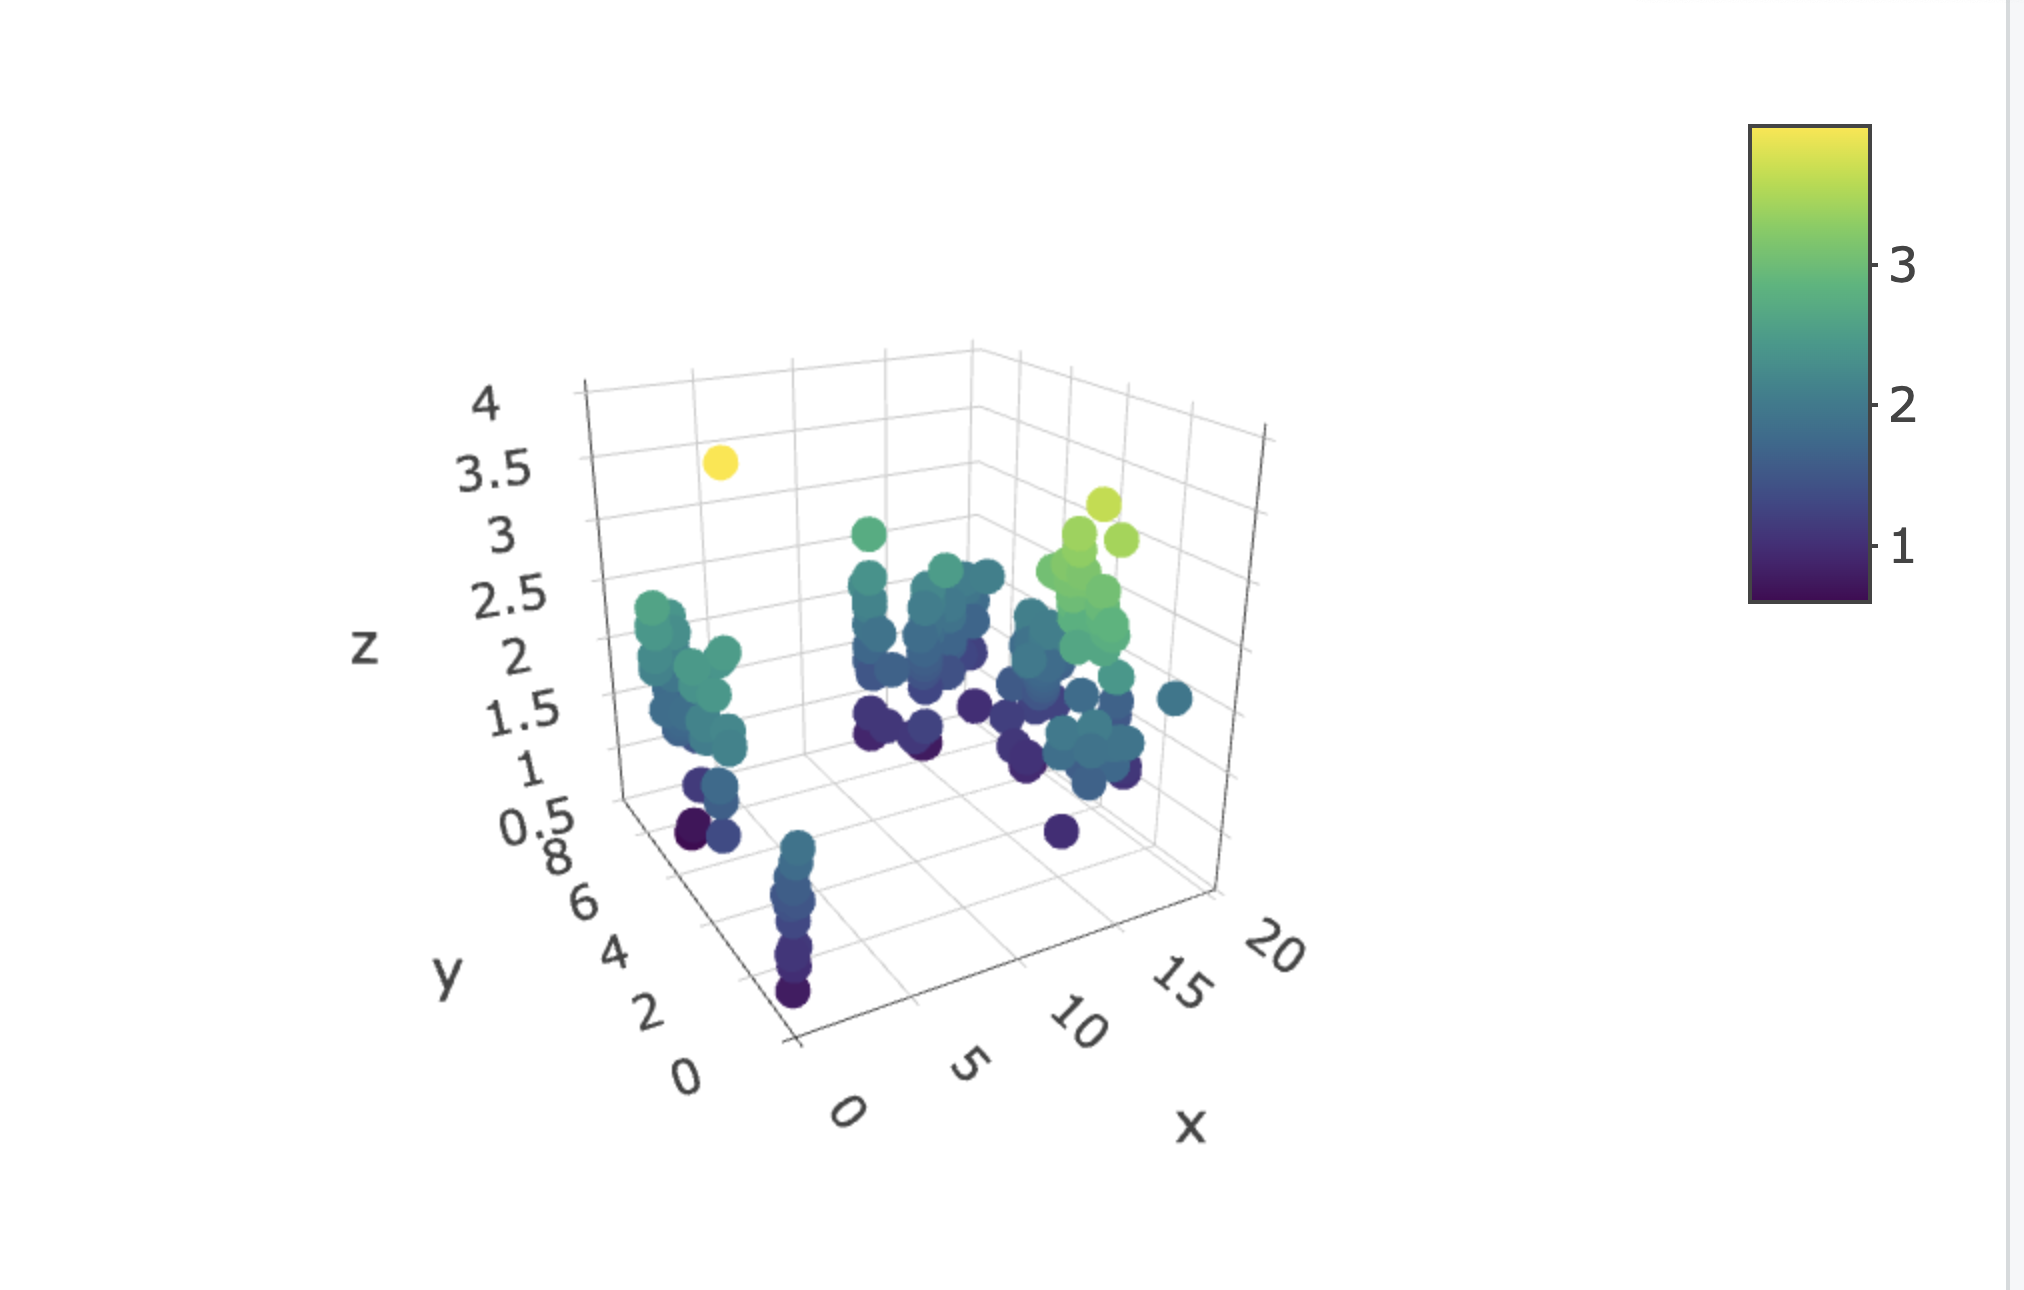
\includegraphics[width=0.85\linewidth,height=\textheight,keepaspectratio]{images/Ls_xyz.png}

}

\caption{\label{fig-tridim}Distribución tri-dimensional de las orquídeas
en los árboles}

\end{figure}%

\begin{enumerate}
\def\labelenumi{\arabic{enumi})}
\setcounter{enumi}{3}
\tightlist
\item
  \textbf{Método de triangulación.} Es un método con área que
  complementa el uso de las técnicas de escalera y de ascenso con una
  cuerda. Se trata de una técnica no invasiva que permite registrar la
  ubicación espacial de las orquídeas sobre los árboles
  (Hernández-Apolinar, 1992). El método consiste en definir el área de
  muestreo (e.g.~20 x 10 m), que corresponde a aquella en la que se
  ubican los árboles con mayor número de orquídeas. Las esquinas del
  cuadro o rectángulo definido se marcan con estacas permanentes y se
  colocan cintas métricas sobre los lados, las cuales se tomarán como
  referencia para ubicar espacialmente a las orquídeas en ejes de
  coordenadas \textbf{x}, \textbf{y}, \textbf{z}, siendo ésta última la
  altura del suelo a la orquídea sobre el tronco o alguna rama. Esta
  técnica tiene cierto grado de dificultad; sin embargo, es muy precisa,
  permite estimar la abundancia de la especie por superficie y se tiene
  la opción de evitar el etiquetado de plantas para su seguimiento.
  Además, en caso de robo de plantas y/o etiquetas es posible reconocer
  con facilidad a los individuos faltantes.
\end{enumerate}

Los árboles tienen una distribución espacial dentro de un área de
muestreo, pero la figura anterior muestra cómo los epífitas se
distribuyen y no es en dos dimensiones solamente. Ese componente
espacial en 3 dimensiones podría influenciar las características
demográficas de los individuos. Por ejemplo, en \emph{Tolumnia
variegata} la planta ubicada en las ramitas más externas (más sol)
versus las del interior del árbol (en la sombra) impacta su esfuerzo
reproductivo (Tremblay, Ackerman \& Pérez, 2010).

\begin{figure}[H]

{\centering 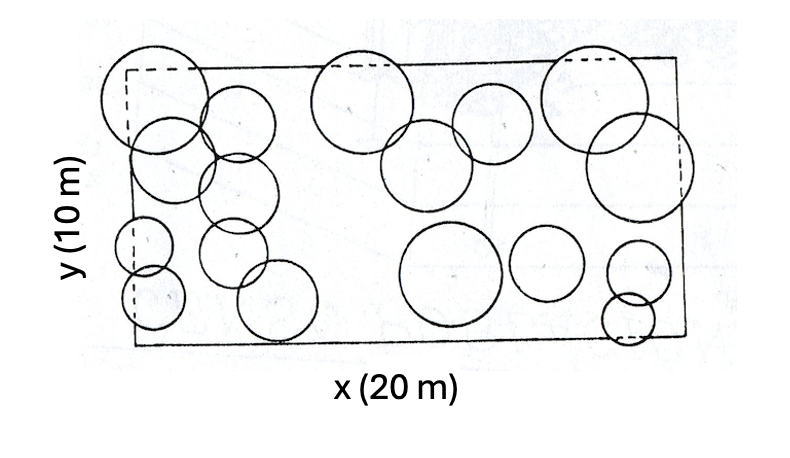
\includegraphics[width=0.85\linewidth,height=\textheight,keepaspectratio]{images/tree_dist.png}

}

\caption{Distribución espacial de los forófitos y el tamaño de cubierta
foliar en el área de muestreo}

\end{figure}%

\subsection{Orquídeas terrestres}\label{orquuxeddeas-terrestres}

En el muestreo de poblaciones de orquídeas terrestres se han
implementado varias técnicas de muestreo. En esta sección nos
referiremos a dos: el método de triangulación y el método sin área. El
primero permite estimar el área en que se establece la población,
mientras que el segundo no permite establecer el área, centrándose en el
marcaje de individuos como se explica a continuación.

\begin{enumerate}
\def\labelenumi{\alph{enumi})}
\tightlist
\item
  \emph{Método de triangulación.} El método de triangulación es una
  técnica no invasiva, comúnmente utilizada para monitorear las
  poblaciones terrestres en Australia (Tremblay et~al., 2009a). El
  método consiste en clavar dos estacas o clavijas permanentes en el
  suelo, formando un cuadro (ver Figura~\ref{fig-triangulation}). La
  distancia entre estaca y estaca generalmente es de un metro (adaptarla
  a su necesidad). Sobre las estacas se puede sobreponer un clavo donde
  se amarran las cintas métricas. Para la ubicación espacial de los
  individuos dentro del cuadro, se usa la distancia de cada planta a
  partir de dos de los lados, en un eje de coordenadas \textbf{x},
  \textbf{y}. Esta técnica es muy buena cuando los individuos están
  separados uno del otro, pero hay que tener cuidado cuando están muy
  cercanos (menos de 1 cm de distancia). Además, es muy precisa, fácil
  de implementar y deja muy poca evidencia en el campo.
\end{enumerate}

\begin{figure}

\centering{

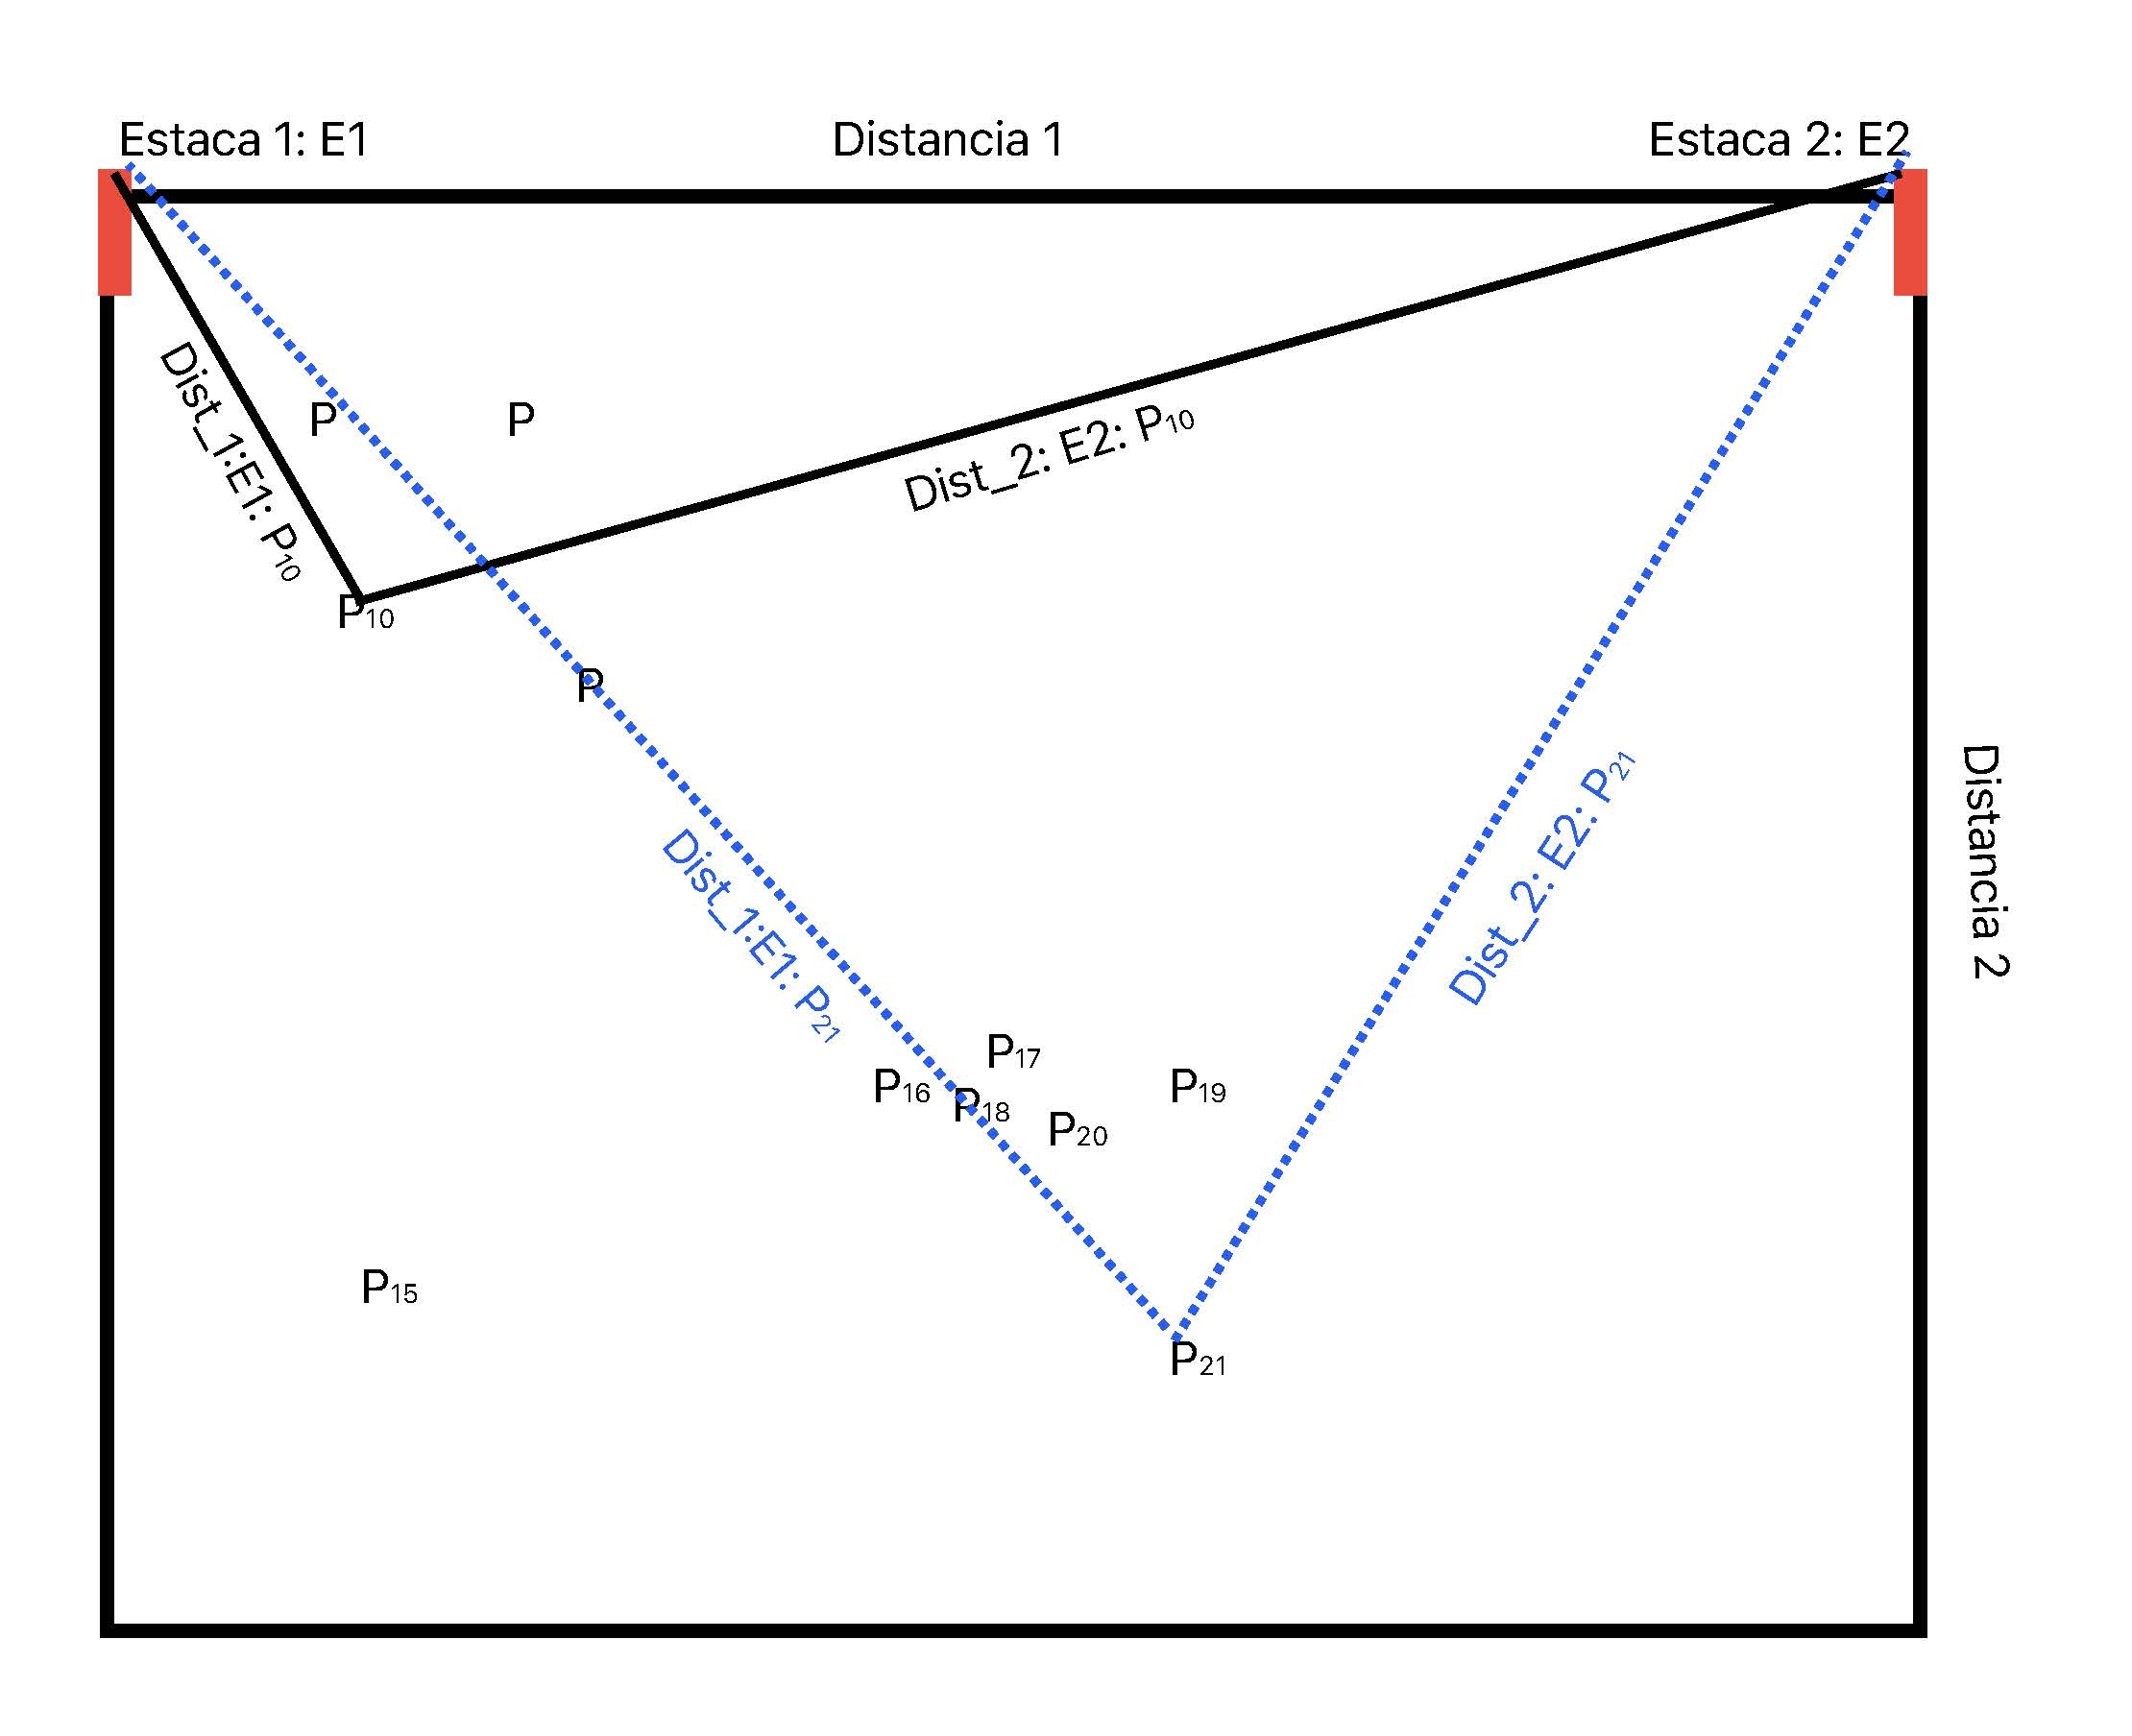
\includegraphics[width=0.7\linewidth,height=\textheight,keepaspectratio]{images/Triangulation_Method.jpg}

}

\caption{\label{fig-triangulation}Método de triangulación para muestreo
terrestre: los P\_x representan la posición de cada planta. Dos
distancias son medidas a partir de cada estaca. Note que este método no
añade un identificador individual a las plantas.}

\end{figure}%

\begin{enumerate}
\def\labelenumi{\alph{enumi})}
\setcounter{enumi}{1}
\tightlist
\item
  \emph{Método sin área.} En el campo, las orquídeas terrestres forman
  pequeñas colonias, e.g.~\emph{Bletia campanulata}, \emph{B.
  macristhmochila}, \emph{Govenia lagenophora}, \emph{Sarcoglottis
  schaffneri} y \emph{Schiedeella albovaginata} (Téllez \& Flores,
  2007); e incluso hay especies con individuos aislados,
  e.g.~\emph{Dichromanthus cinnabarinus}, \emph{D. aurantiacus} (Téllez
  \& Flores, 2007), \emph{Cypripedium irapeanum} (Hernández-Apolinar
  et~al., 2012) y \emph{Govenia lagenophora} (Hernández-Apolinar,
  Gutiérrez-Paredes \& Luis, 2012), por lo que su dinámica poblacional
  generalmente se describe a partir de la información obtenida en varias
  colonias o subpoblaciones. El método sin área ha sido ampliamente
  usado en este tipo de orquídeas, no es invasivo y consiste en la
  selección de una colonia o subpoblación en la que se marcan todas las
  plantas observadas en el lugar (Martı́nez-Villegas et~al., 2024).
  Asimismo, la ubicación de los sitios y los individuos puede
  georreferenciarse y/o hacer mapas de localización.
\end{enumerate}

\begin{center}\rule{0.5\linewidth}{0.5pt}\end{center}

\section{Marcaje y monitoreo de los individuos en el
tiempo}\label{marcaje-y-monitoreo-de-los-individuos-en-el-tiempo}

La dinámica o cambio en una población se evalúa marcando y siguiendo a
todos los individuos que se encuentran en un sitio (i.e.~censo) o de
solo una parte de éstos (i.e.~muestreo) entre periodos de tiempo
(típicamente anual) a lo largo de sus distintas etapas de desarrollo
(i.e.~semillas, plántulas, juveniles y adultos). Sin importar si
censamos o muestreamos, tenemos que asegurar tres aspectos durante el
marcaje o etiquetado de una población.

\begin{tcolorbox}[enhanced jigsaw, arc=.35mm, bottomrule=.15mm, bottomtitle=1mm, breakable, colback=white, colbacktitle=quarto-callout-important-color!10!white, colframe=quarto-callout-important-color-frame, coltitle=black, left=2mm, leftrule=.75mm, opacityback=0, opacitybacktitle=0.6, rightrule=.15mm, title=\textcolor{quarto-callout-important-color}{\faExclamation}\hspace{0.5em}{Importante}, titlerule=0mm, toprule=.15mm, toptitle=1mm]

\textbf{Tres condiciones que debe cumplir cualquier marcaje.}

\begin{enumerate}
\def\labelenumi{\arabic{enumi}.}
\tightlist
\item
  \textbf{Cobertura de etapas:} se incluyan individuos de todas las
  categorías que conforman la población.
\item
  \textbf{Tamaño de muestra suficiente:} suficientes individuos para que
  el análisis demográfico refleje la dinámica real de la población, y no
  ruido de muestreo.
\item
  \textbf{Registro libre de error:} sistema de codificación claro,
  consistente y trazable que minimice errores en campo y en el análisis
  posterior.
\end{enumerate}

\end{tcolorbox}

\begin{center}\rule{0.5\linewidth}{0.5pt}\end{center}

\subsection{Identificación y etiquetado de
individuos}\label{identificaciuxf3n-y-etiquetado-de-individuos}

Debido a la naturaleza sésil de las plantas, una vez delimitada la
población resulta relativamente sencillo contar e identificar a todos
los individuos en su estado juvenil y adulto, si se toma en cuenta su
aspecto morfológico similar y la presencia o ausencia de estructuras
reproductivas (i.e.~flores, inflorescencias y/o frutos; ver Sección
\hyperref[sec-etapas-orquideas]{Etapas o estados de desarrollo en
orquídeas}). Sin embargo, la identificación y monitoreo de semillas y
plántulas es muy difícil de lograr en campo, de ahí que señalemos las
dos siguientes consideraciones:

\begin{enumerate}
\def\labelenumi{\alph{enumi})}
\item
  \emph{Semillas.} La fase de semillas es uno de los mayores retos en el
  estudio de las orquídeas, ya que su tamaño tan pequeño (i.e.~son
  conocidas como semillas polvo o ``dust-seeds'') dificulta el
  seguimiento de su dispersión y germinación en el campo (Ackerman,
  Sabat \& Zimmerman, 1996; Ticktin et~al., 2020). La evaluación de
  ambos procesos es de gran utilidad en los estudios poblacionales al
  momento de estimar los valores de fecundidad o de transición al primer
  estadio del ciclo de vida. El método más usado para evaluar la
  germinación en el medio natural es la introducción de bolsas pequeñas
  de malla de plancton (Rasmussen \& Whigham, 1993; Rasmussen, 2011;
  Anghelescu et~al., 2023). Estas bolsas son selladas y contienen un
  número de semillas definido que posteriormente se colocan en el suelo
  o sobre los árboles (e.g.~ramas, tronco) y se recogen en uno o
  distintos periodos del año a fin de evaluar la germinación y el
  establecimiento de nuevos individuos (Emeterio-Lara et~al., 2016).
\item
  \emph{Plántulas.} El seguimiento e identificación de plántulas en
  campo ha sido poco abordado debido a la dificultad para encontrarlas
  (especialmente en especies terrestres) y por el desconocimiento de su
  morfología en la gran mayoría de las orquídeas. Estas condiciones han
  limitado la estimación de parámetros poblacionales como la
  supervivencia y la transición a la fase juvenil (Emeterio-Lara \&
  Damon, 2024). Durante el muestreo en el bosque XXXX en el año
  \#\#\#\#, de \emph{Cypripedium irapeanum}, una orquídea terrestre, se
  encontró un número muy limitado de plántulas en el campo (ver
  Figura~\ref{fig-cirap-plantula}). Estos individuos tuvieron una talla
  pequeña y además presentaron una morfología distinta a la de un
  adulto, al ser tallos muy delgados y de apariencia semejante al de un
  pasto. Durante su búsqueda se hurgó principalmente alrededor de las
  plantas juveniles y adultas de la misma especie, ya que varias se
  ubicaron en esta zona.
\end{enumerate}

\begin{figure}

\centering{

\pandocbounded{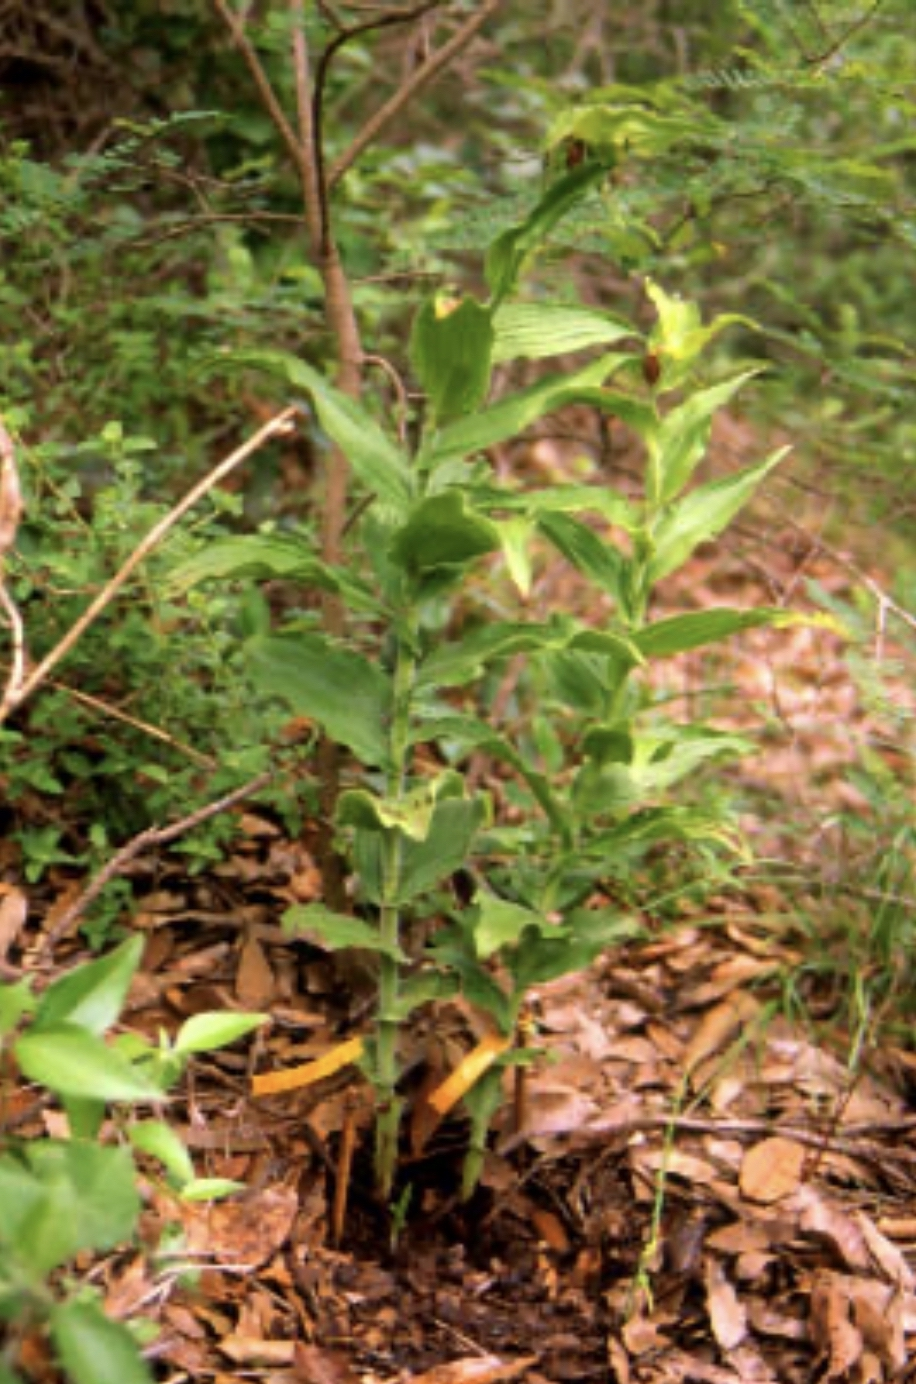
\includegraphics[keepaspectratio]{images/C_irap_plantula.jpeg}}

}

\caption{\label{fig-cirap-plantula}Plántula de \emph{Cypripedium
irapeanum}. Foto: Claudia Gutiérrez-Paredes}

\end{figure}%

Las plántulas son los individuos más pequeños en la población de
orquídeas epífitas, las cuales pueden no reconocerse con facilidad al
estar cubiertas de musgo y liquen. Tremblay (com. pers.) ha encontrado a
estas pequeñas plantas alrededor de las plantas adultas, por lo que
recomienda esta estrategia de búsqueda en esta fase de desarrollo.
Cuando más de una especie del mismo género comparte el mismo hospedero,
la identificación se complica; por ejemplo, en el caso de las plántulas
de \emph{Lepanthes} (ver Figura~\ref{fig-lep-woodburyana}) se establecen
entremezcladas en el mismo forófito y carecen de caracteres distintivos
en esta etapa, por lo que es imposible distinguirlas por especie
(Tremblay \& Hutchings, 2003); esto se logra únicamente cuando se marcan
y siguen cuidadosamente a etapas posteriores (juvenil o adulto).

\begin{figure}

\centering{

\pandocbounded{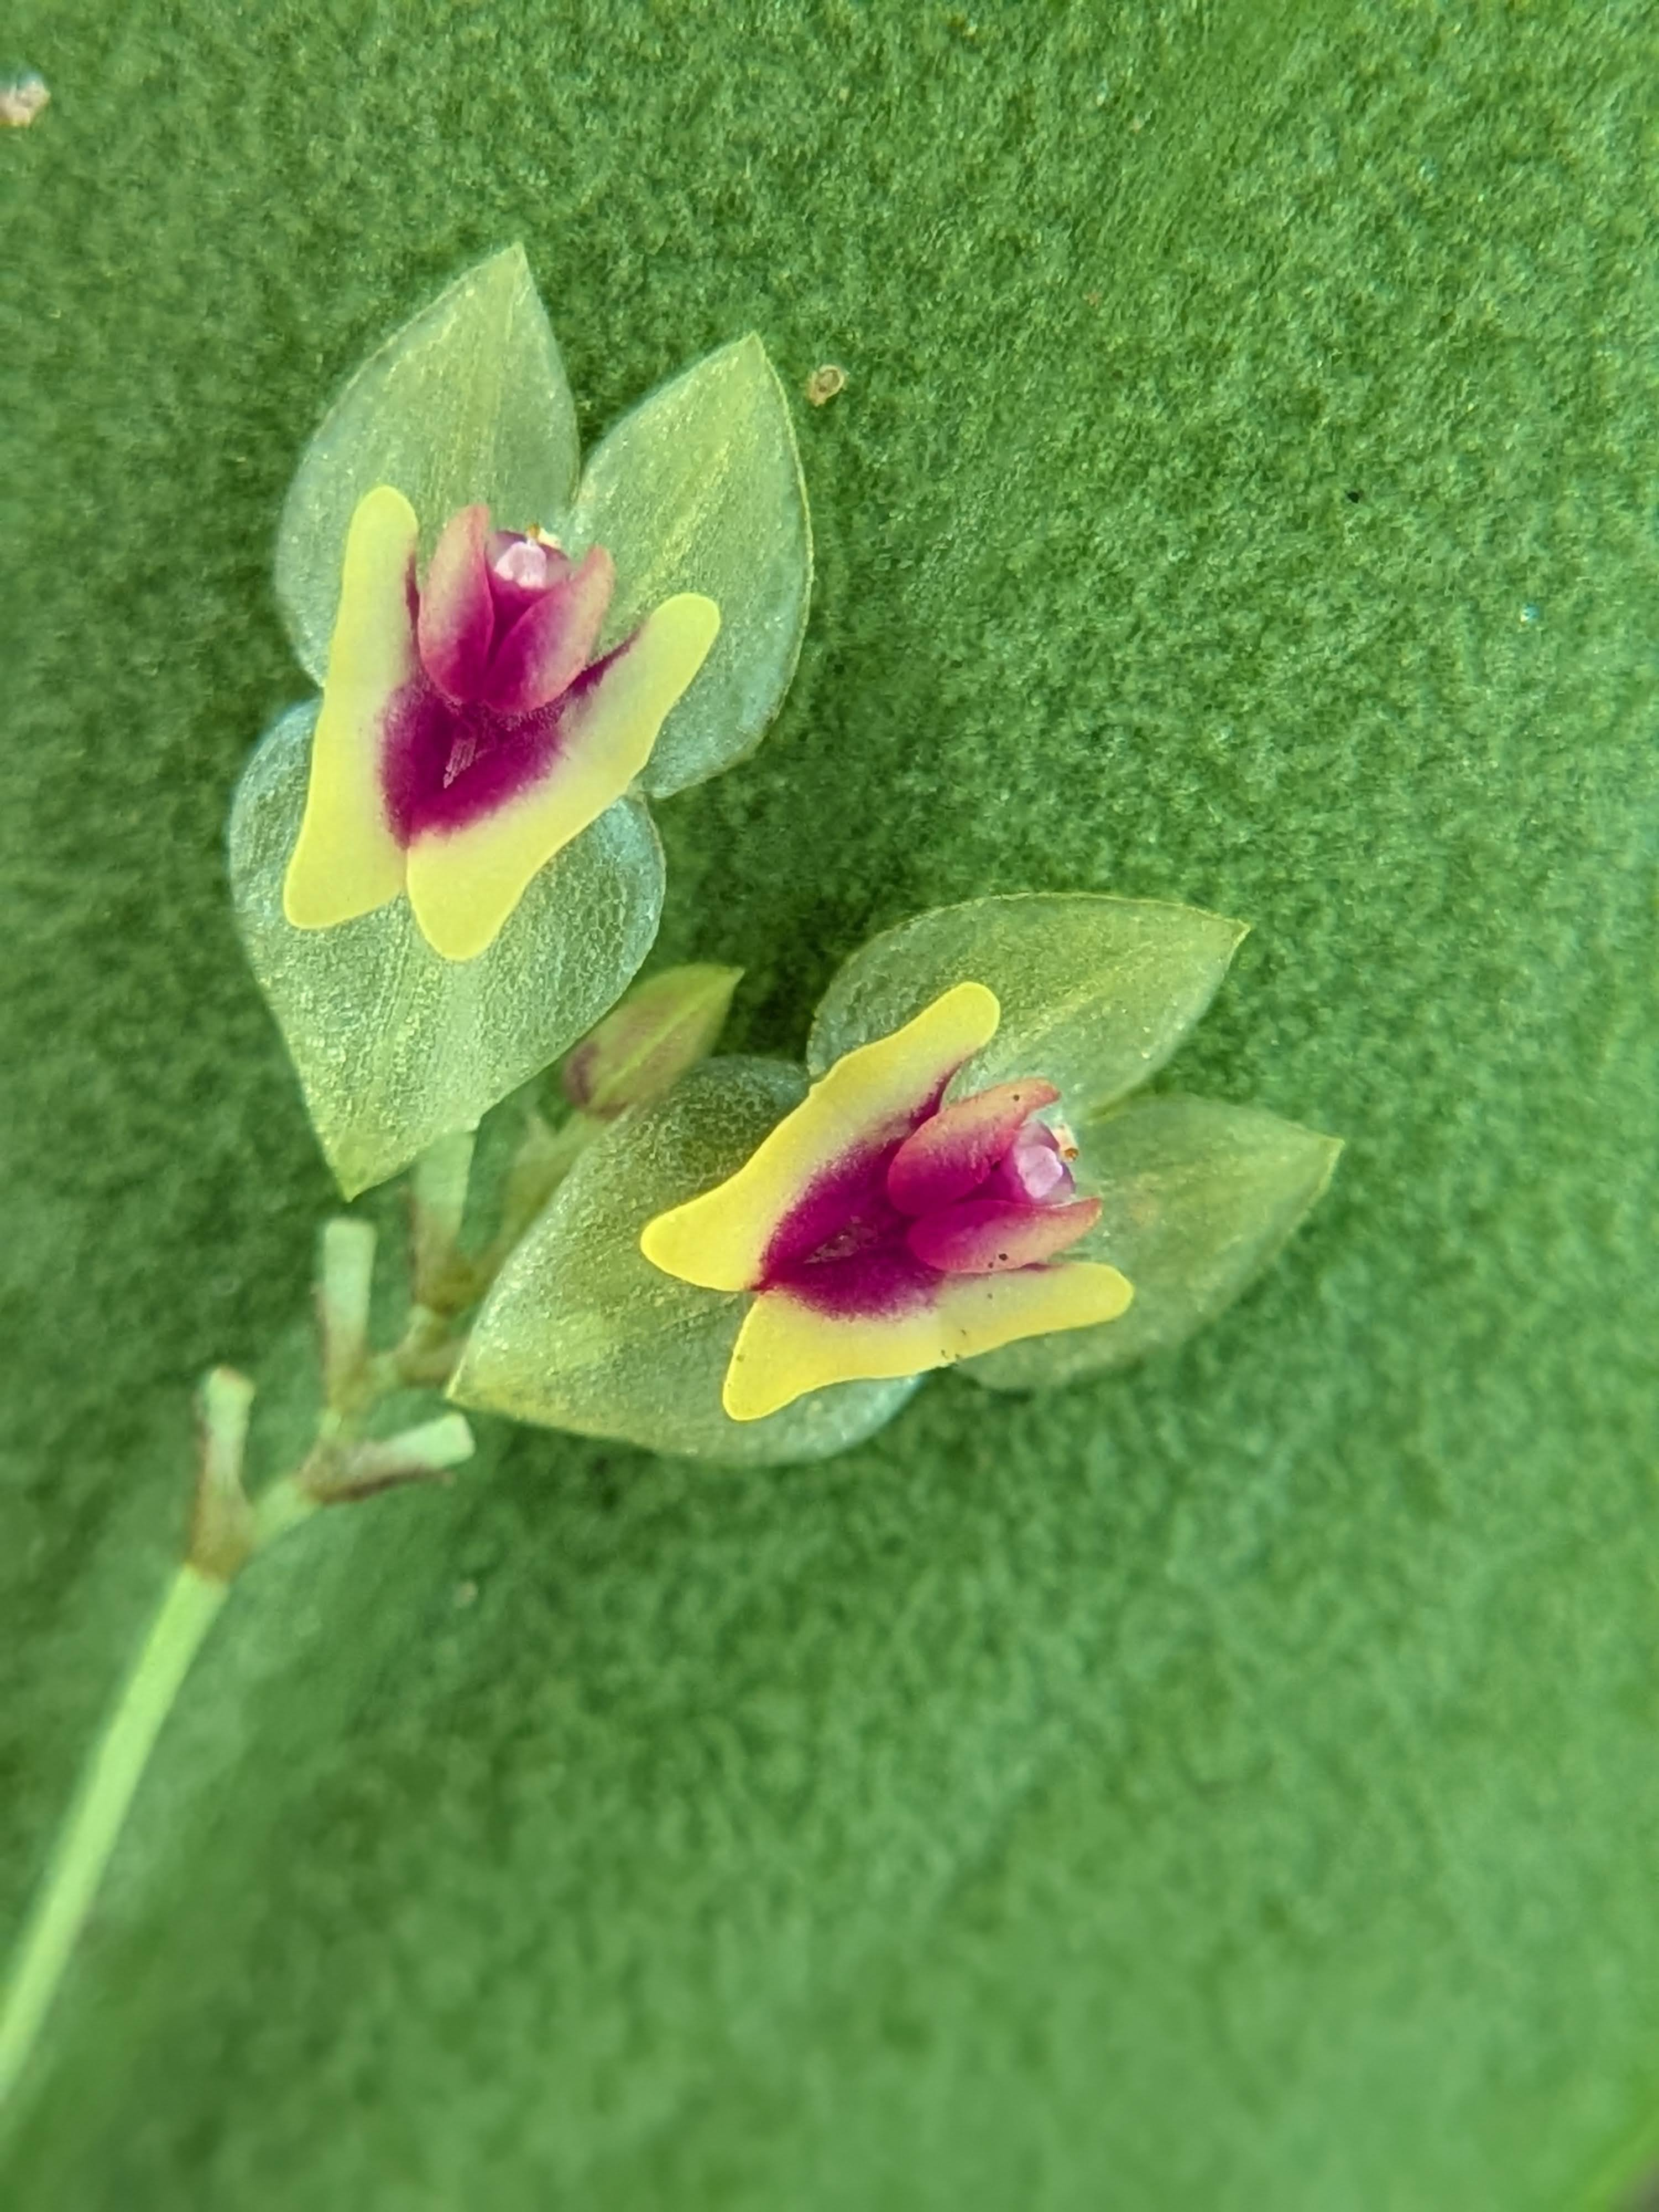
\includegraphics[keepaspectratio]{images/Lepanthes_woodburyana.jpg}}

}

\caption{\label{fig-lep-woodburyana}\emph{Lepanthes woodburyana}. Foto:
Edwin Guevara}

\end{figure}%

A través de esta estrategia (ver Figura~\ref{fig-lep-woodburyana}), el
autor ha logrado distinguir entre plántulas de \emph{Lepanthes
eltoroensis} y \emph{L. woodburyana}, las cuales se diferencian en la
forma de crecimiento del tallo. Al continuar el desarrollo,
\emph{Lepanthes eltoroensis} tendrá un crecimiento postrado, mientras
que será erecto en \emph{L. woodburyana}. Si bien este método es bueno,
es importante considerar que puede representar un periodo de tiempo
largo y que se corre el riesgo de no poder reconocer la especie cuando
las plántulas no sobreviven a la siguiente etapa o el estudio termina
antes que las plántulas crezcan a la próxima etapa.

\section{Identificación de las etapas de la especie con
facilidad}\label{identificaciuxf3n-de-las-etapas-de-la-especie-con-facilidad}

Para cualquier estudio usando el acercamiento de dinámica poblacional es
necesario conocer lo básico de la especie de interés y las etapas/edades
que correspondan al ciclo de vida de esa misma especie y que sean
representativas de su historia de vida. Poder reconocer las diferentes
etapas del ciclo de vida con exactitud es esencial; por ejemplo, separar
entre las semillas, plántulas, juveniles y adultos (diferentes tamaños
de adultos) y si hay etapas latentes. Cuando se define una etapa de vida
se deberían tener características morfológicas que se puedan identificar
en el campo con facilidad para reducir los errores de asignaciones a
otras etapas. Por ejemplo, en el caso de \emph{Lepanthes} (ver
Figura~\ref{fig-lep-rupestris}) (Tremblay \& Hutchings, 2003) se definió
un juvenil como individuo que tiene tallos con vaina lepanthiforme
(\emph{lepanthiform sheath}) en por lo menos uno de los pecíolos y que
no tiene evidencia presente o anteriormente de inflorescencias. Note que
aquí la diferencia entre una plántula y un juvenil es que tenga una
vaina lepanthiforme y se diferencia de los adultos por la ausencia de
evidencia de inflorescencias seca y activa.

Veamos algunos ejemplos a continuación. Por ejemplo, en la
Figura~\ref{fig-lep-rupestris} tenemos un individuo que tiene dos hojas,
una con inflorescencia activa y la otra hoja con inflorescencia seca;
por tal razón ese individuo es un adulto, ya que tiene por lo menos una
inflorescencia activa (produciendo flores o tiene el potencial de
producir flores). Note que no es que la inflorescencia tenga flores, es
que la inflorescencia es verde (el potencial de producir flores). Hay
que reconocer que la vida de una flor puede ser muy corta y que el
muestreo es puntual, y que no todas las flores se van a poder
contabilizar (por ejemplo, en algunas especies de \emph{Lepanthes} las
plantas florecen todo el año). Debido a que no todas las flores se
pueden evaluar cuando están abiertas para remoción del polinio (esfuerzo
reproductivo masculino) o deposición de polen sobre el estigma (esfuerzo
reproductivo femenino), se puede contabilizar la cantidad de flores
contando las cicatrices de la inflorescencia.

\begin{center}\rule{0.5\linewidth}{0.5pt}\end{center}

\section{Etiquetado de individuos}\label{etiquetado-de-individuos}

Los cambios en abundancia (i.e.~número de individuos) de las poblaciones
y los procesos biológicos que influyen sobre ésta se estiman a partir
del monitoreo y secuenciación de todos y cada uno de los procesos o
eventos por los que transitan los individuos en cada estado de un
periodo a otro (e.g.~un mes o un año). Esto es sólo posible cuando
contamos con material de marcaje de calidad y un sistema de
identificación sencillo y claro.

Estos dos sencillos pasos evitarán mezclar la información entre
individuos de una misma población o confundir la información con plantas
de otras poblaciones o periodos de tiempo. Es decir, la calidad de
nuestros datos dependerá, en parte, de cómo marquemos y de qué calidad
sea el material que usemos para el marcaje.

\begin{center}\rule{0.5\linewidth}{0.5pt}\end{center}

\subsection{Material recomendado para marcar o etiquetar un individuo o
sitio de
muestreo}\label{material-recomendado-para-marcar-o-etiquetar-un-individuo-o-sitio-de-muestreo}

La calidad y la durabilidad del material de marcaje es muy importante
cuando hacemos un estudio poblacional, más aún cuando se trata de uno de
largo plazo. Si las marcas se desintegran de un periodo a otro, se
perderá la identidad de cada planta y si no nos damos cuenta podríamos
suponer dos cosas en nuestro siguiente monitoreo: i) que el individuo
murió (al no aparecer la etiqueta), o ii) que hay un nuevo reclutamiento
en la población (aparece un nuevo individuo sin marca). Esto sesgaría
nuestros resultados al suponer un aumento en la mortalidad o, en su
defecto, un aumento en el reclutamiento. Naturalmente, ese sesgo
dependerá del número de individuos que marquemos (i.e.~tamaño de la
muestra). Por regla general se ha considerado que a menor tamaño de
muestra, mayor es el sesgo.

\begin{tcolorbox}[enhanced jigsaw, arc=.35mm, bottomrule=.15mm, bottomtitle=1mm, breakable, colback=white, colbacktitle=quarto-callout-warning-color!10!white, colframe=quarto-callout-warning-color-frame, coltitle=black, left=2mm, leftrule=.75mm, opacityback=0, opacitybacktitle=0.6, rightrule=.15mm, title=\textcolor{quarto-callout-warning-color}{\faExclamationTriangle}\hspace{0.5em}{Advertencia}, titlerule=0mm, toprule=.15mm, toptitle=1mm]

\textbf{Una etiqueta perdida sesga dos parámetros a la vez.} Si la marca
se desintegra entre censos, el individuo aparece como muerto
(sobreestima la mortalidad) y vuelve a aparecer como nuevo recluta en el
siguiente período (sobreestima el reclutamiento). El sesgo es
proporcionalmente mayor en muestras pequeñas. Por eso conviene invertir
desde el inicio en material durable (cinta de \emph{dymo}, aluminio
laminado) y un protocolo de re-etiquetado conservador.

\end{tcolorbox}

Las etiquetas de \emph{dymo} (ver Figura~\ref{fig-cypripedium-acaule})
resultan ser un buen material al marcar los individuos de las orquídeas
de cualquier tipo de crecimiento (i.e.~epífito, terrestre o rupícola).
Este material ha resultado ser muy duradero en sistemas tropicales; por
ejemplo, fueron legibles después de más de 15 años de haber marcado a
individuos de \emph{Lepanthes} (Tremblay com. pers.). Por otro lado, el
aluminio laminado es otro material barato y duradero sobre el cual se
puede escribir fácilmente, por lo que se garantiza la permanencia de la
marca o etiqueta y la de las inscripciones que hayamos hecho sobre ésta.
Además, este tipo de etiquetas, al igual que las de \emph{dymo}, pueden
sujetarse a la planta o colocarse cerca de ésta con diferentes
materiales; por ejemplo, hilo de pescador, cinchos de plástico, alambre
galvanizado o plastificado, clavos, chinchetas y grapas, entre los más
usados (ver Figura~\ref{fig-laelia-cincho}). Un aspecto que hay que
cuidar al marcar individuos es que las etiquetas se enmascaren con el
ambiente; es decir, que no sean muy grandes, que estén protegidas y que
no sean evidentes para todos, a fin de evitar su pérdida o, incluso, el
robo de plantas por gente ajena a la investigación.

\begin{figure}

\centering{

\pandocbounded{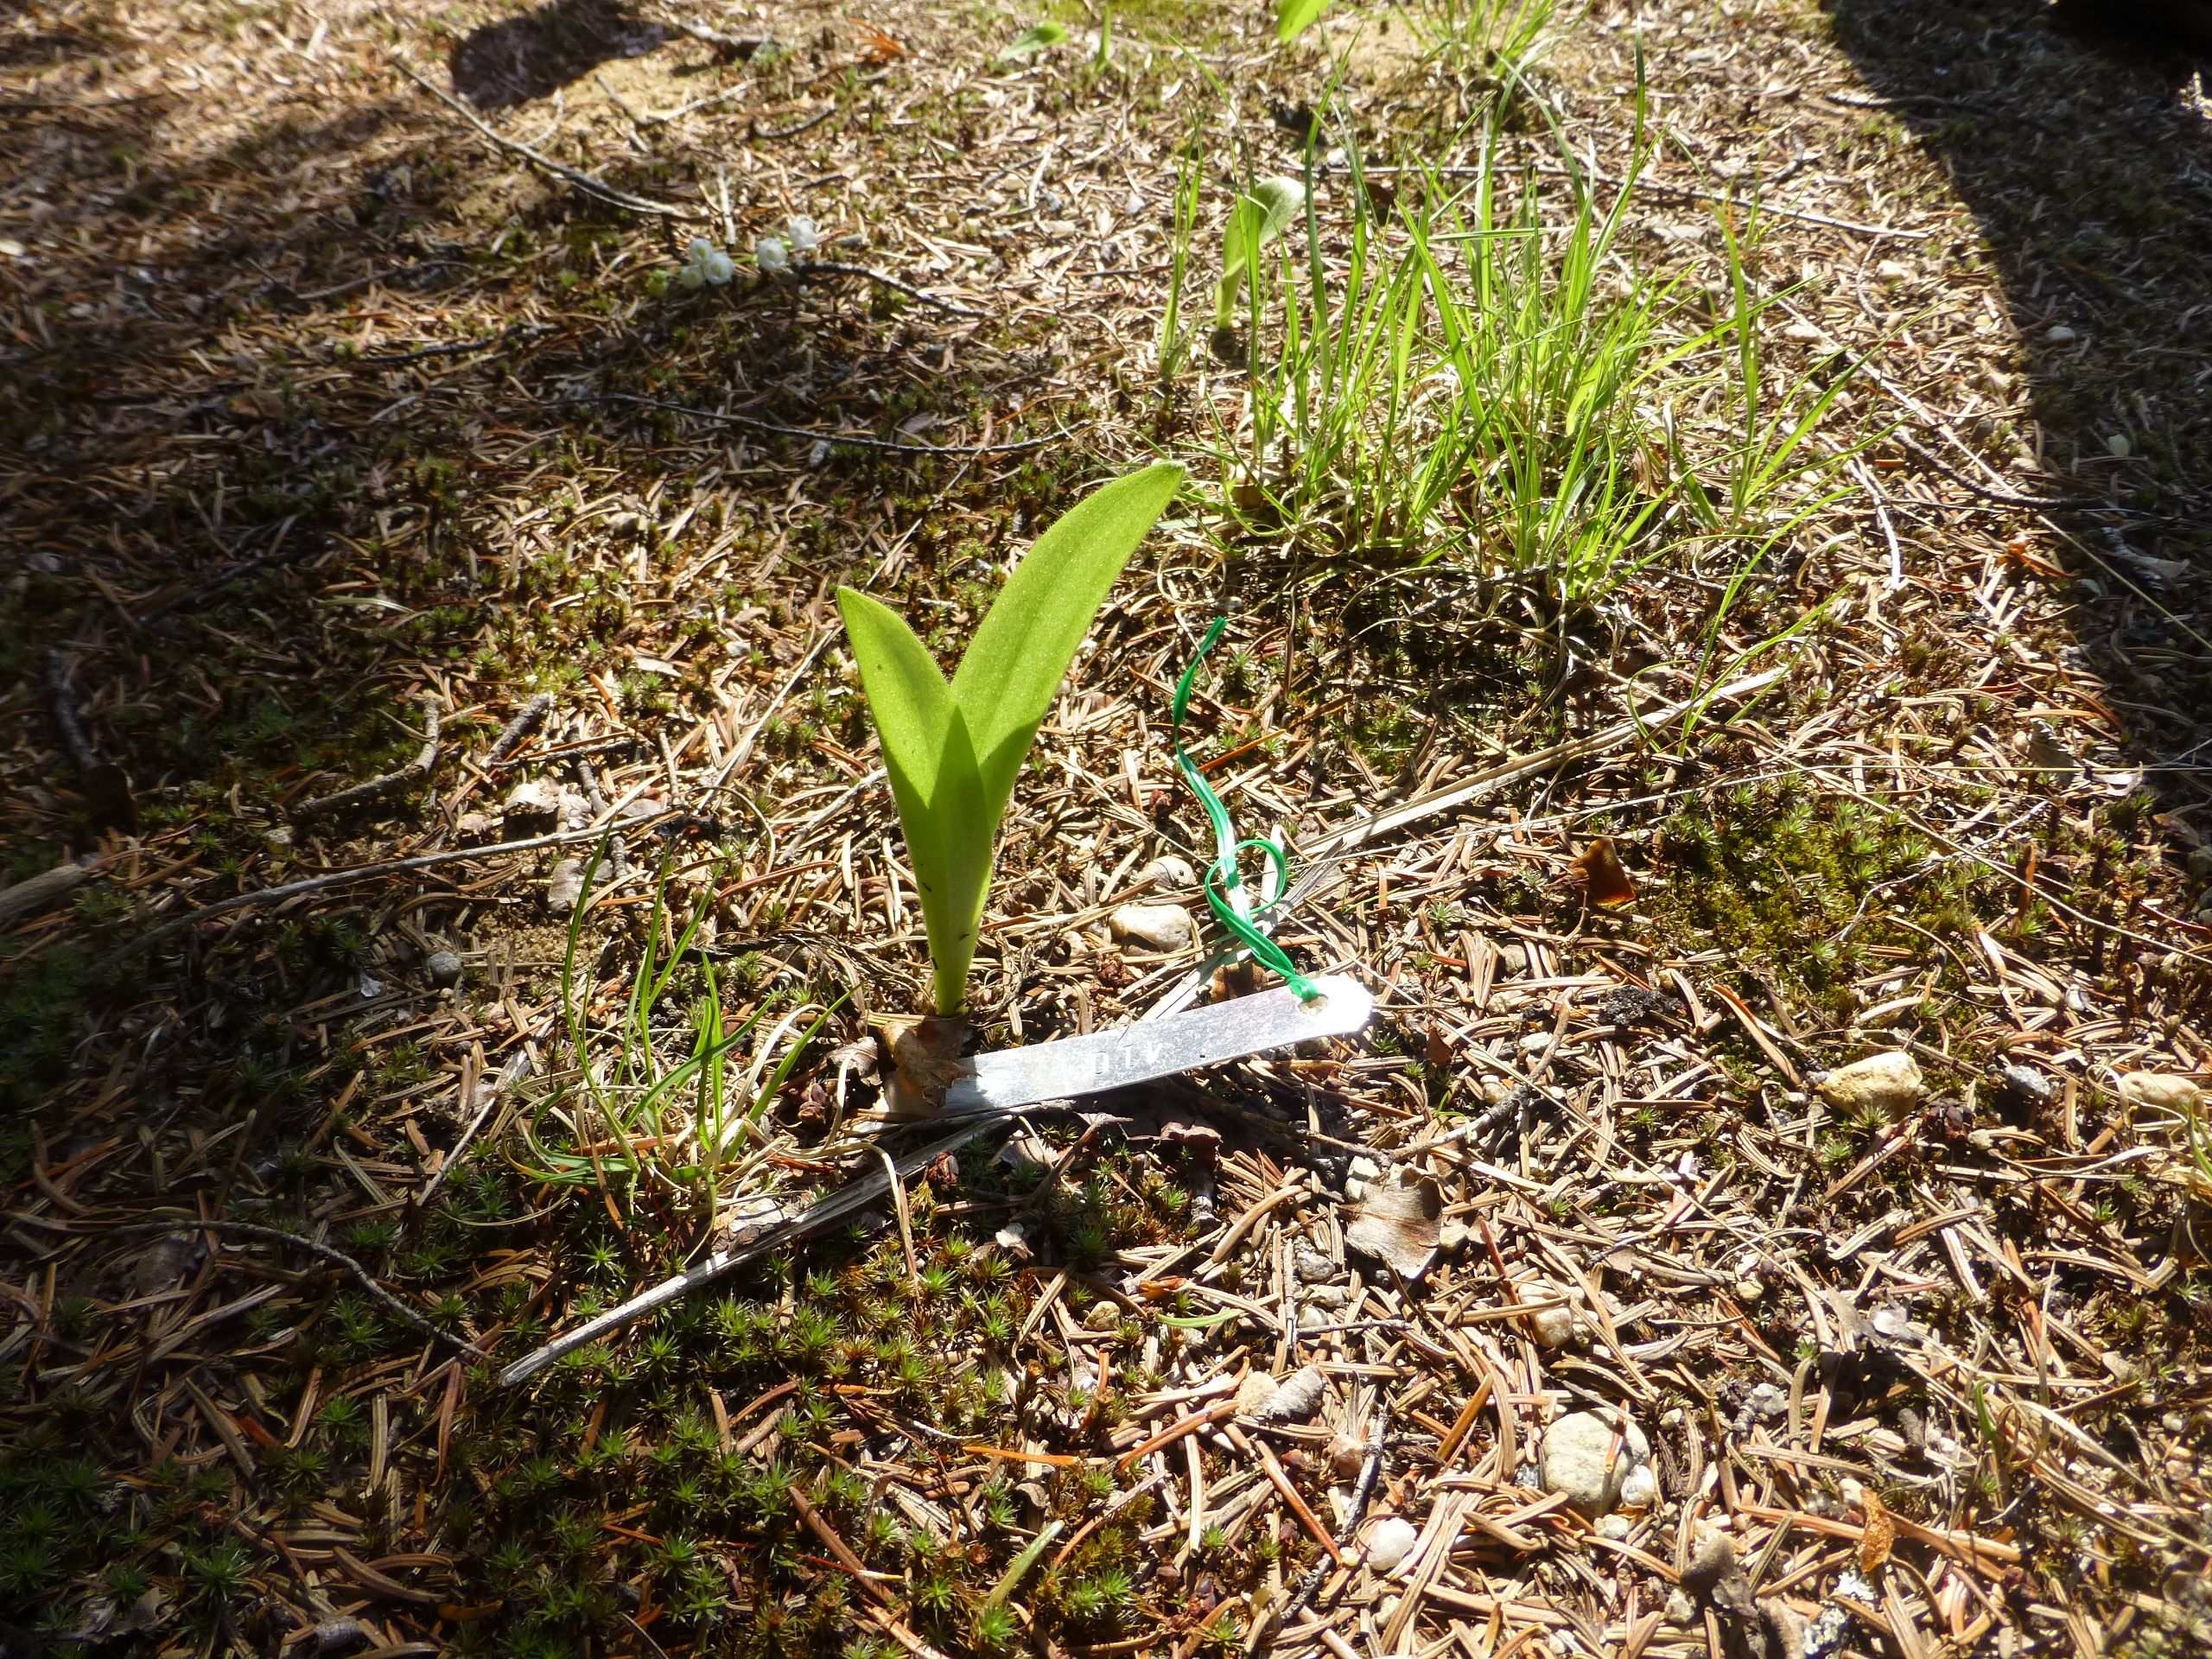
\includegraphics[keepaspectratio]{images/Cypripedium_acaule.jpg}}

}

\caption{\label{fig-cypripedium-acaule}Uso de etiquetas de aluminio en
marcaje de \emph{Cypripedium acaule}. Foto: Tremblay}

\end{figure}%

\begin{figure}

\centering{

\pandocbounded{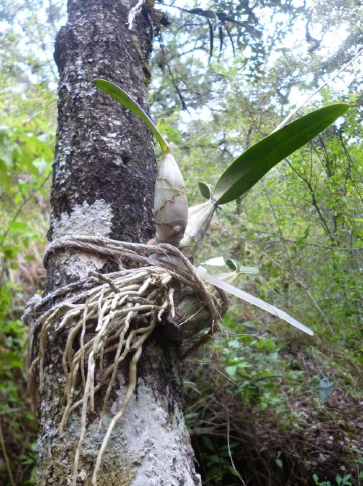
\includegraphics[keepaspectratio]{images/Laelia_cincho.png}}

}

\caption{\label{fig-laelia-cincho}Uso de etiquetas de aluminio en
marcaje con cinchos de plástico en \emph{Laelia autumnalis}. Foto por
Aucencia Emeterio-Lara}

\end{figure}%

La durabilidad del material usado es muy importante cuando existen
eventos en el ciclo de vida de una especie que pueden prolongarse por
varios años. Este es el caso de algunas orquídeas terrestres que pueden
no rebrotar y mantenerse en latencia vegetativa por más de un ciclo
anual de forma consecutiva. Por ejemplo, la latencia vegetativa puede
durar un periodo consecutivo de tres años en \emph{Liparis liliifolia}
(Hutchings, 1987; Wells, 1991), cinco a siete años en \emph{Epipactis
helleborine} (Coates, Lunt \& Tremblay, 2006; Light \& MacConaill,
2006), e incluso ser mayor en \emph{Prasophyllum correctum} (Coates,
Lunt \& Tremblay, 2006). Es así que una buena secuenciación de estos
eventos en un individuo en el mediano y largo plazo depende de la
calidad del material usado al marcar las plantas, lo cual a su vez
permitirá tener buenas estimaciones del tamaño poblacional y la
supervivencia y reproducción en la población.

Al igual que los individuos, los sitios de muestreo también se marcan a
fin de facilitar su ubicación en el medio natural. Estos pueden ser
marcados usando banderines, etiquetas grandes de aluminio o plástico,
cinta de señalización (\emph{flagging tape}) o pintura permanente;
asimismo, también se pueden georreferir y hacer mapas de localización.

Cuando se trata de marcas de colores, se deben preferir colores poco
llamativos camuflajeados con la vegetación circundante. Si el sitio está
bien protegido se puede optar por colores fuertes y llamativos; sin
embargo, hay que considerar que los animales (mamíferos, aves,
herbívoros) pueden ser atraídos por las marcas e ingerirlas o
destruirlas (a ciertas orugas les gusta la cinta de \textbf{dymo} y
dejan su evidencia), de ahí que se sugiera utilizar etiquetas discretas
que favorezcan su permanencia en el mediano y largo plazo. Es sumamente
importante poner el máximo esfuerzo en el muestreo consistente entre
periodos y tratar de encontrar todos los individuos previamente
marcados.

\begin{center}\rule{0.5\linewidth}{0.5pt}\end{center}

\subsection{Información básica en una
etiqueta}\label{informaciuxf3n-buxe1sica-en-una-etiqueta}

La marca o etiqueta de cada uno de los individuos de una población debe
compactar la mayor cantidad de información posible, no solo números
consecutivos. Es decir, generalmente escribimos números consecutivos (1,
2, 3, 4, etc.) en las etiquetas que colocamos a cada individuo en campo.
Sin embargo, si no hay notas guía, esta información es limitada cuando
se retoma la investigación en campo, ya que es difícil determinar cuándo
ingresaron los nuevos individuos a la población o cuándo se fragmentó
una planta para dar origen a un individuo de una categoría distinta al
de plántula. Asimismo, si se seleccionan distintas poblaciones o
colonias y los números consecutivos son los mismos, podemos confundir la
información y llegar a conclusiones erróneas.

Cuando se estudia una sola población, una forma sencilla de evitar
errores y anexar más información es escribir en la etiqueta el año de
estudio y el número consecutivo de la planta. Por ejemplo, si el estudio
comenzó en 2023 y la población está formada por 152 individuos
(i.e.~captura), éstos se podrían codificar así: 23001, 23002, 23003,
\ldots{} 23152. En el siguiente año (2024) se revisarán o censarán los
152 individuos originalmente marcados (i.e.~recaptura) y se etiquetarán
los nuevos individuos que ingresan a la población (e.g.~plántulas), cuya
marca iniciará con 24 y el número consecutivo (153 en adelante). De esta
forma se conocerá el año de ingreso, marcaje e inicio de la captura de
datos del individuo, lo cual evitará la redundancia en el código y
ayudará a reducir los errores de identificación.

Cuando la orquídea de interés no tiene una distribución regular y tiene
una distribución aparchonada (concentrada en un área) en distintas zonas
de un mismo lugar, para evitar errores de codificación se sugiere que en
cada parche se mantengan números consecutivos (23001, 23002, 23003,
etc.) y se evite mezclar los números asignados (23001, 23012, 23043,
etc.). Esta misma regla se mantiene cuando se trabaja con distintas
poblaciones de la misma especie.

Otra forma de codificar las múltiples poblaciones o subpoblaciones es a
través de una codificación alfanumérica, en la que la letra del alfabeto
representa a la población y el número a los individuos marcados para su
monitoreo. De esta manera, las marcas individuales se verían de la
siguiente forma: A23001, A23002, \ldots, A23xxx para la primera
población y B23001, B23002, \ldots, B23xxx para la segunda población y
así sucesivamente, en caso de estudiar más de dos poblaciones. Una
tercera opción es asignar un número a cada población y añadir el número
consecutivo correspondiente. En este caso las etiquetas de las plantas
número 10 en dos sitios se verían de la siguiente manera: 1.10 y 2.10.
Si queremos añadir el año del estudio, éste también puede ser al final y
sería de la siguiente forma: 1.10.23 y 2.10.23. Para los nuevos ingresos
se sigue la misma lógica del inciso anterior, por lo que a la nueva
planta 155 que ingresa en 2024 a la población 1 le corresponderá la
etiqueta 1.155.24.

\begin{tcolorbox}[enhanced jigsaw, arc=.35mm, bottomrule=.15mm, bottomtitle=1mm, breakable, colback=white, colbacktitle=quarto-callout-tip-color!10!white, colframe=quarto-callout-tip-color-frame, coltitle=black, left=2mm, leftrule=.75mm, opacityback=0, opacitybacktitle=0.6, rightrule=.15mm, title=\textcolor{quarto-callout-tip-color}{\faLightbulb}\hspace{0.5em}{Recomendación}, titlerule=0mm, toprule=.15mm, toptitle=1mm]

\textbf{Una buena etiqueta es un identificador estructurado, no un
número correlativo.} Conviene combinar tres componentes: año de marcaje
+ número consecutivo + identificador de población. Por ejemplo,
\texttt{A23001} (población A, año 2023, individuo 001) o
\texttt{1.10.23} (población 1, planta 10, año 2023). Esta convención
permite reconocer de inmediato cuándo entró el individuo al estudio, a
qué población pertenece y evita colisiones cuando hay múltiples sitios.

\end{tcolorbox}

\begin{center}\rule{0.5\linewidth}{0.5pt}\end{center}

\subsection{Colocación de la
etiqueta}\label{colocaciuxf3n-de-la-etiqueta}

Existen distintas formas de colocar las etiquetas o marcas en los
individuos seleccionados para el estudio y, por regla general, su
ubicación no debe afectar el desempeño de la planta marcada y se debe
asegurar su permanencia en el mediano y largo plazo. Por ejemplo, en las
orquídeas epífitas de tamaño grande, la etiqueta de identidad se puede
colocar abrazando a la planta, incluyendo la rama o tronco donde se
desarrolla, o bien, colocarse abrazando a uno solo de los módulos. En el
caso de \emph{Laelia autumnalis} (Emeterio-Lara et~al., 2021), además de
la etiqueta de identificación, se identificó con otra etiqueta el último
módulo (el más joven o reciente) de cada uno de los frentes de
crecimiento (ver Figura~\ref{fig-laelia-speciosa-marcaje}). Este tipo de
marcaje permitió determinar la biomasa nueva que se agrega cada año a
cada planta y, al mismo tiempo, permitió identificar la permanencia,
crecimiento o retrogresión entre fases de crecimiento.

\begin{figure}

\centering{

\pandocbounded{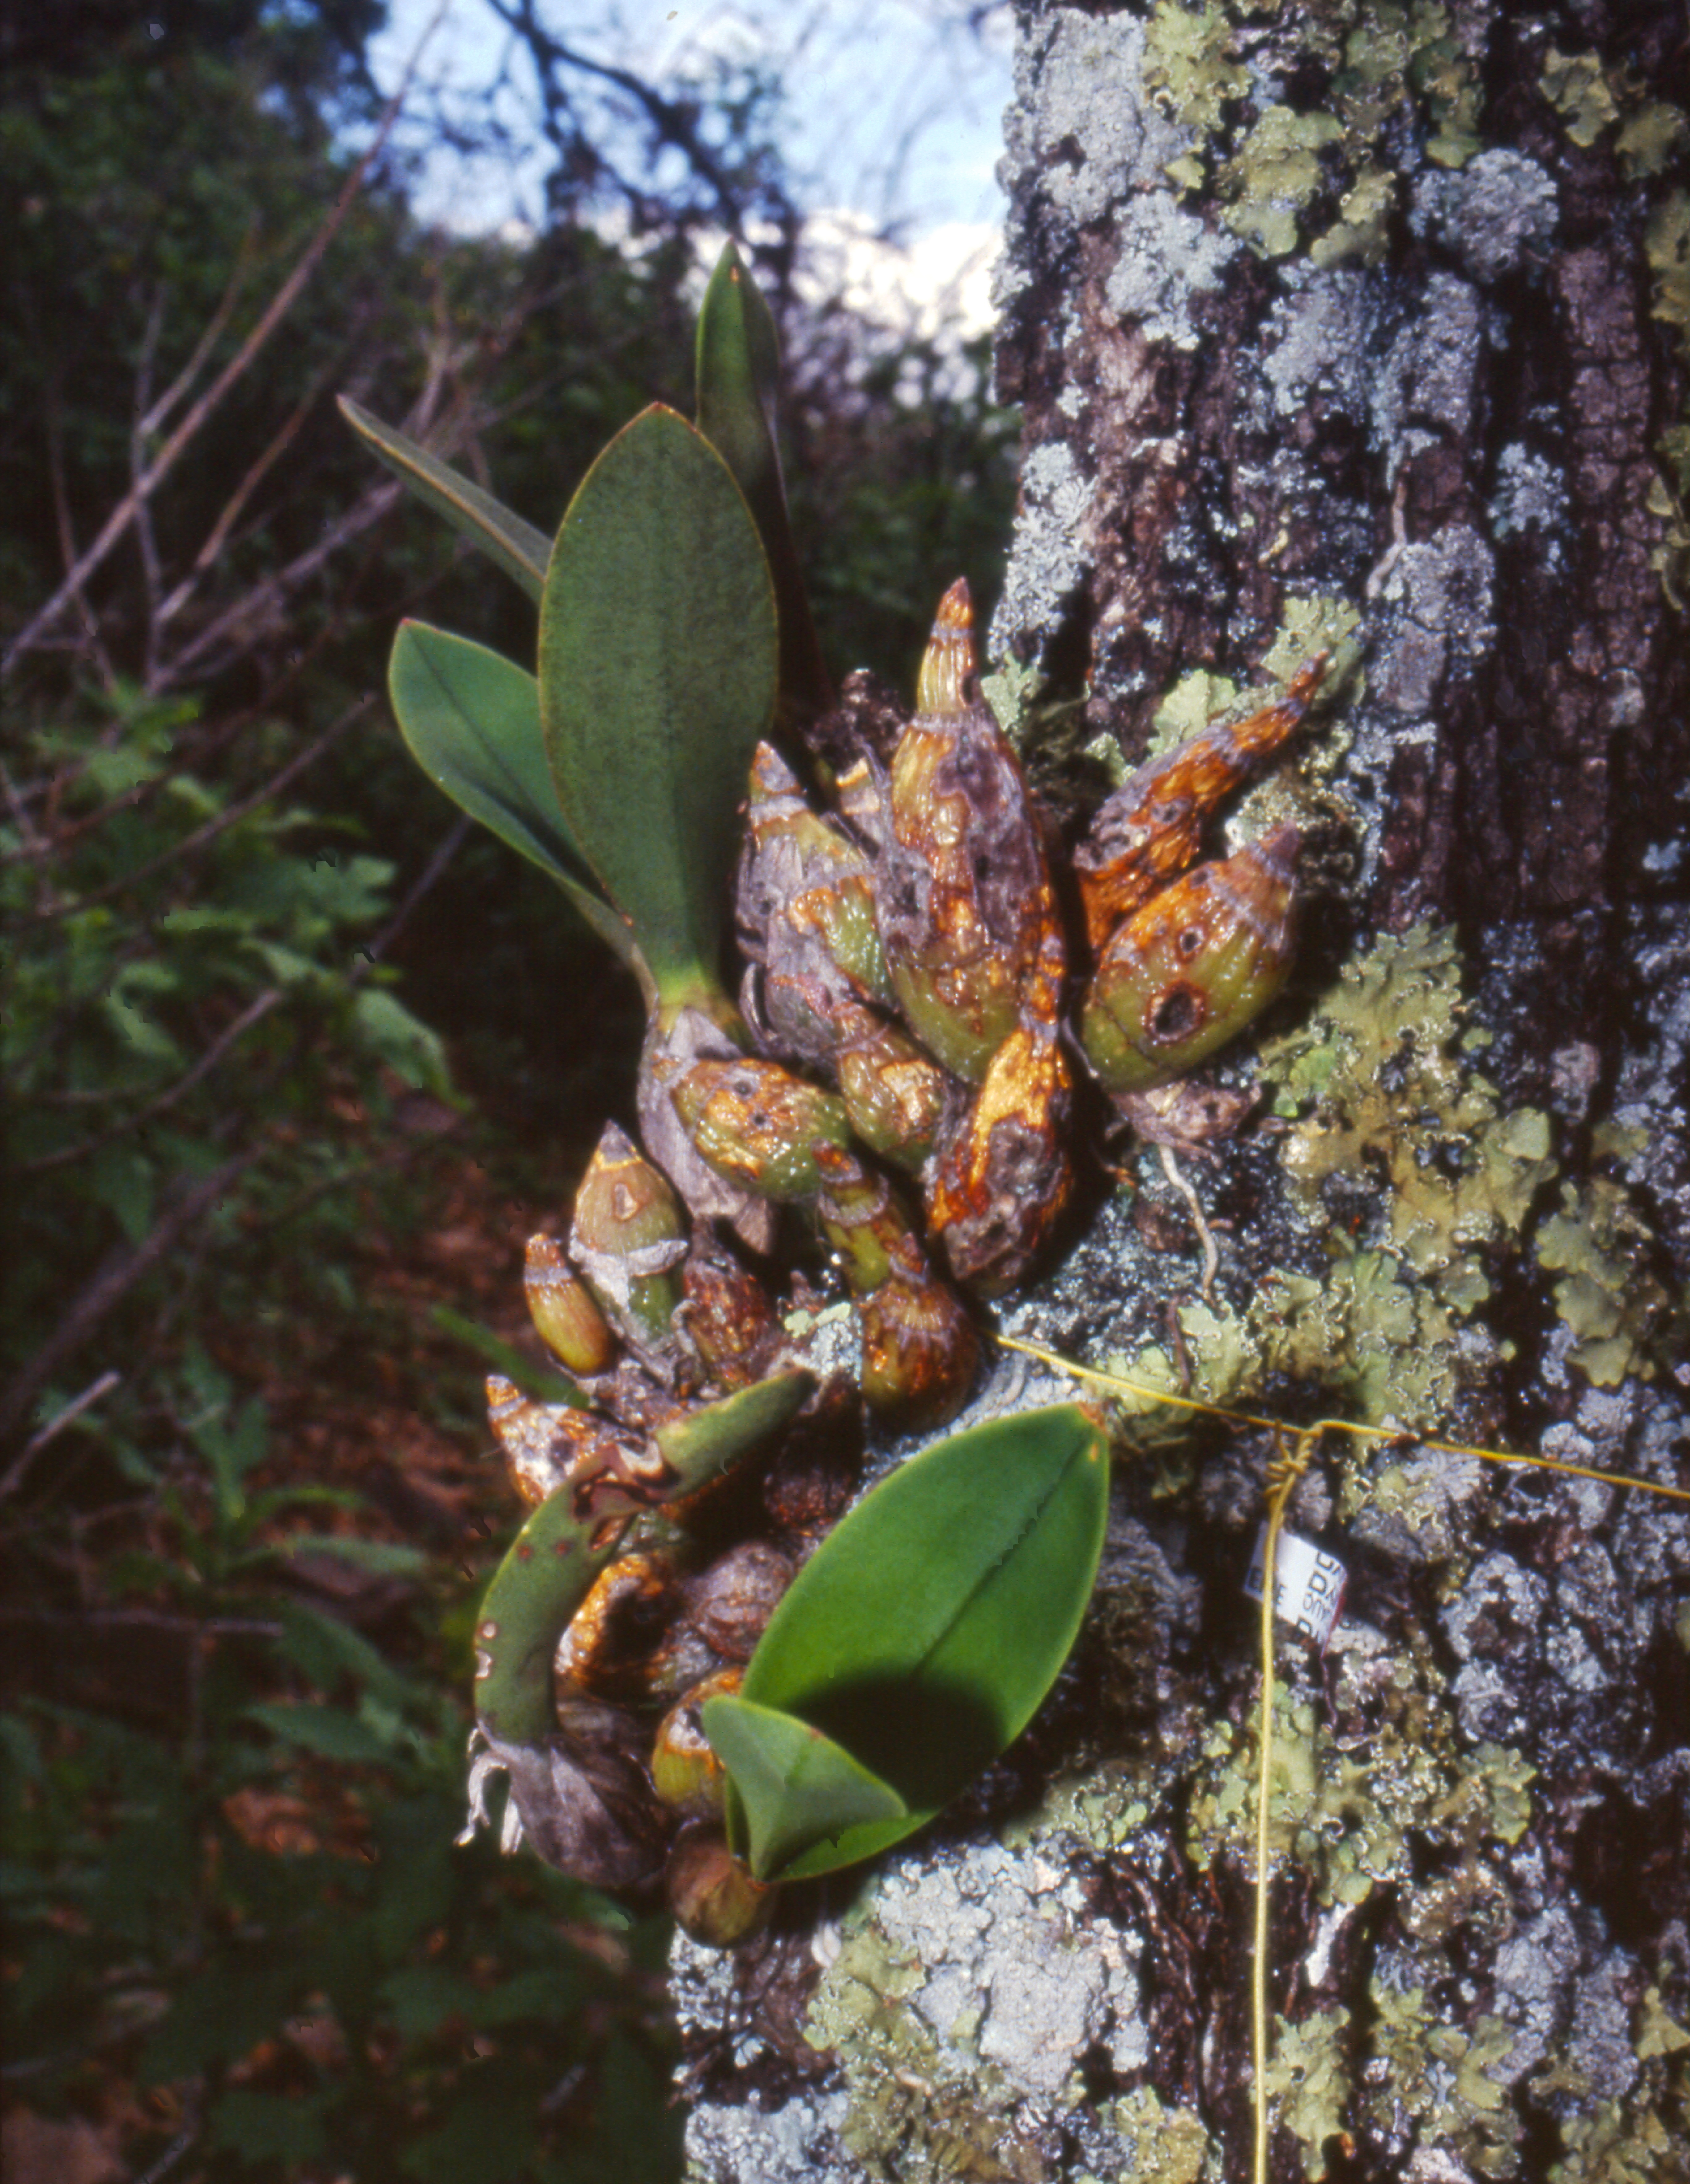
\includegraphics[keepaspectratio]{images/alambrelaelia.jpg}}

}

\caption{\label{fig-laelia-speciosa-marcaje}Marcaje de \emph{Laelia
speciosa} abrazando el tronco con alambre plastificado y etiquetas de
\emph{dymo}. Foto: Mariana Hernández-Apolinar}

\end{figure}%

Las plántulas son muy frágiles, por lo que para no dañar sus estructuras
se debe contar con material suave y, preferentemente, se debe evitar el
contacto con las plantas. En \emph{Lepanthes eltoroensis}, Tremblay fijó
las etiquetas a un lado de las plántulas con clavos pequeños y
posteriormente cambió a grapas, que causan menos daño al árbol hospedero
(ver Figura~\ref{fig-lep-eltoroensis}).

\begin{figure}

\centering{

\pandocbounded{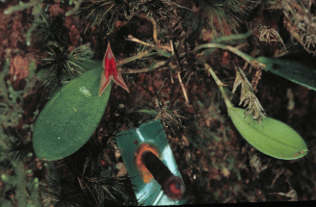
\includegraphics[keepaspectratio]{images/Lep_eltoroensis.png}}

}

\caption{\label{fig-lep-eltoroensis}Los individuos de \emph{Lepanthes
eltoroensis} fueron identificados con una etiqueta de plástico clavada
al tronco del árbol; posteriormente las nuevas etiquetas fueron
engrapadas a la corteza del árbol. Foto: Tremblay}

\end{figure}%

En las orquídeas terrestres \emph{Cypripedium irapeanum} y \emph{Govenia
lagenophora} las etiquetas de aluminio o cinta \textbf{dymo} fueron
amarradas con alambre plastificado a palos o clavos, semejando
banderitas, que luego fueron clavadas en el suelo cerca de los tallos o
pseudobulbos de las plantas (ver Figura~\ref{fig-cirap-marcaje} y
Figura~\ref{fig-cyp-acaule-flag}).

\begin{figure}

\centering{

\pandocbounded{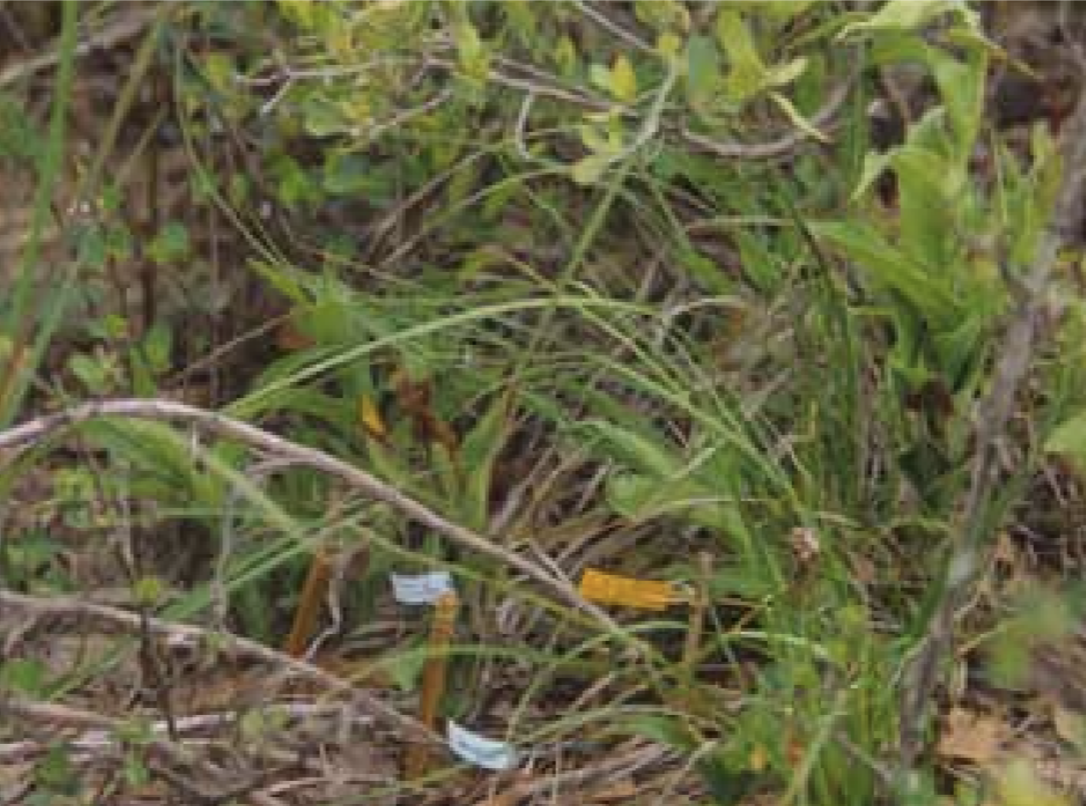
\includegraphics[keepaspectratio]{images/Cirap_marcaje.png}}

}

\caption{\label{fig-cirap-marcaje}Marcaje de \emph{Cypripedium
irapeanum} con cinta de \emph{dymo}. Foto: Hernández-Apolinar}

\end{figure}%

\begin{figure}

\centering{

\pandocbounded{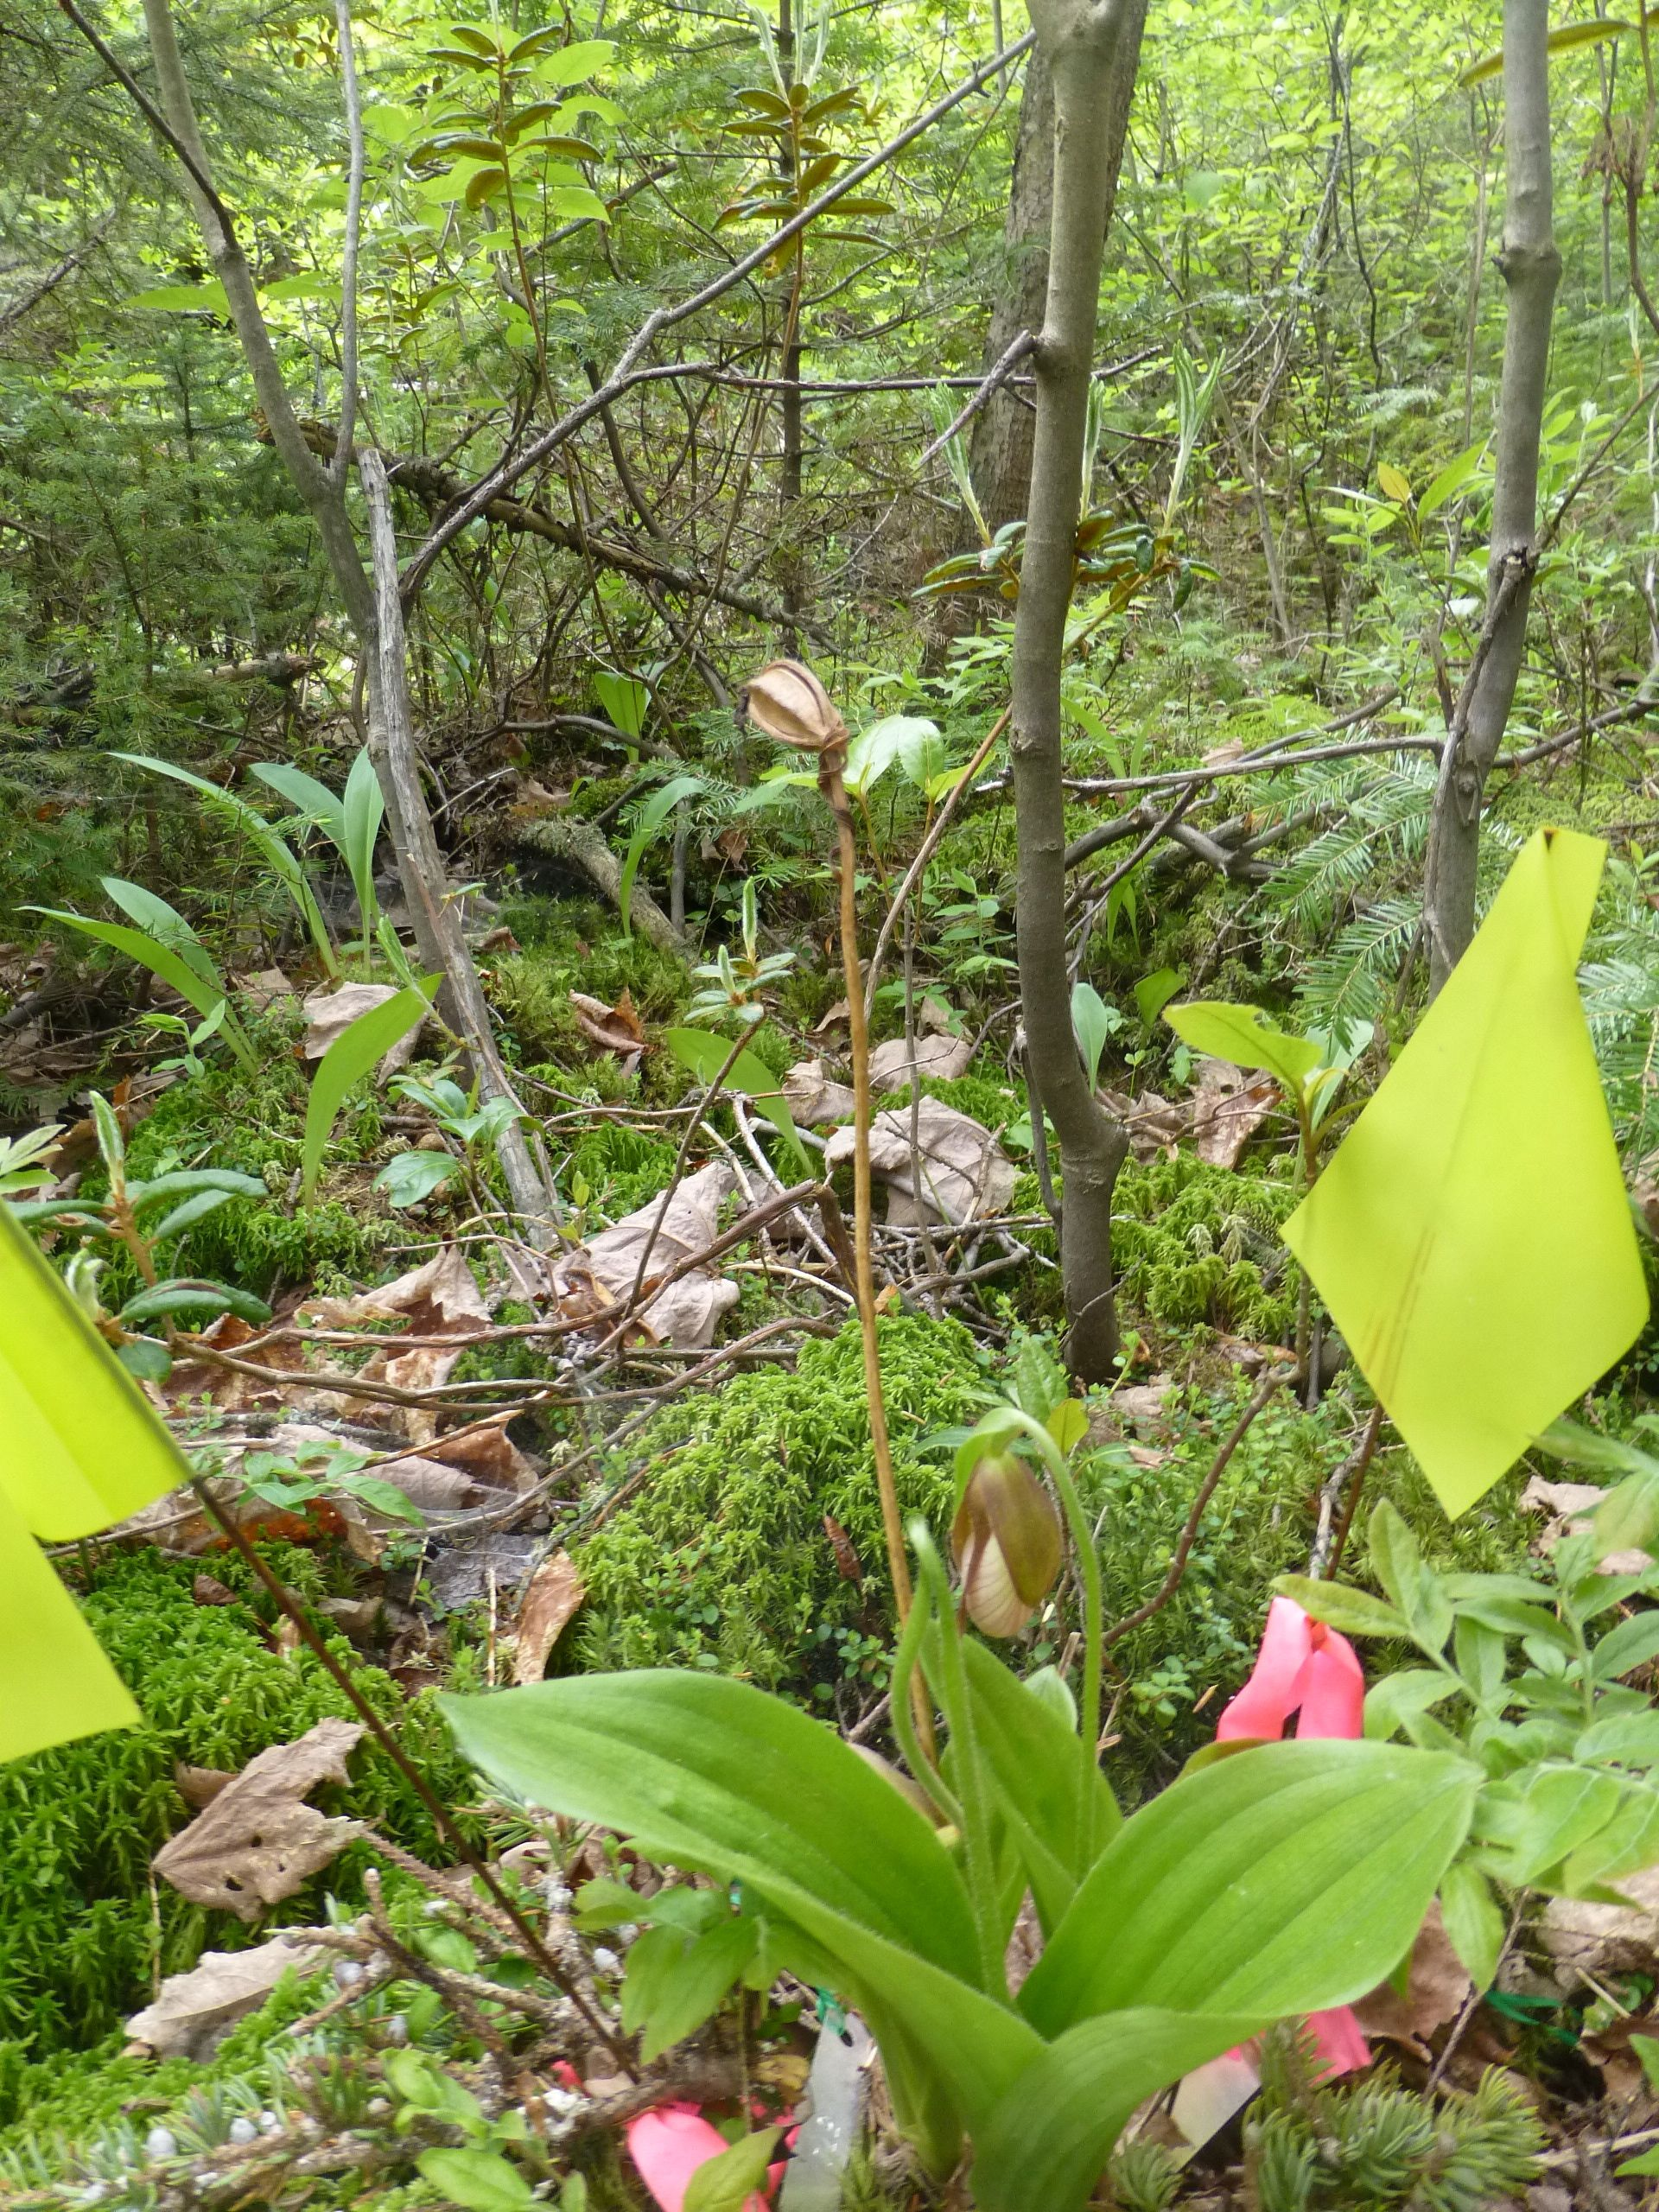
\includegraphics[keepaspectratio]{images/Cyp_acaule_flag.jpg}}

}

\caption{\label{fig-cyp-acaule-flag}Marcaje de \emph{Cypripedium acaule}
con banderitas. Foto: Tremblay}

\end{figure}%

\begin{center}\rule{0.5\linewidth}{0.5pt}\end{center}

\section{Variables a identificar en
campo}\label{variables-a-identificar-en-campo}

En esta sección se presentan algunos ejemplos de cómo se ha dividido la
estructura poblacional en orquídeas con distinto hábito de crecimiento.
A través de los ejemplos es evidente que las categorías de etapa/estado
no siempre son las mismas en las especies, ya que dependen de aspectos
biológicos de las plantas (e.g.~características morfológicas, de
crecimiento, de reproducción), de la información disponible, del número
de individuos marcados y de las preguntas de interés en la investigación
(Hernández-Apolinar, 1992; Mondragón \& Elliott, 2013).

No importa las variables que usemos en la clasificación de las plantas,
lo que se captura es información relevante en las especies, la cual es
común en todos los estudios poblacionales por estados
(Tabla~\ref{tbl-variables-censo}). La primera información se obtiene al
inicio del estudio, definido como el tiempo cero o inicial \(t_{0}\) y
se refiere a las características básicas más simples que permiten
diferenciar un estadio de otro, mientras que los siguientes periodos de
toma de datos, denominados como \(t_{+1}\) (i.e.~n = 2, 3, 4, \ldots{}
n), permiten entender los cambios que ocurren en los individuos de un
periodo a otro (i.e.~crecen, se reproducen, viven o mueren) y, además,
captar de dónde provienen los nuevos individuos que ingresan a la
población (i.e.~semilla, origen vegetativo o clonación) en el periodo
\(t_{+n}\).

Las variables esenciales (Tabla~\ref{tbl-variables-censo}), junto con
las características definidas en cada etapa de desarrollo (ver
\hyperref[sec-ejemplos-categorizacion]{Ejemplos de categorización}),
permiten conocer, por un lado, cuál o cuáles de las categorías son muy
dinámicas o, por el contrario, constantes en el ciclo de vida de la
especie de interés; y por otro, el estado de conservación de la
población en su conjunto. Esta última se define a partir de la tasa
finita de crecimiento poblacional como se establece en el Capítulo
\emph{XX}.

\global\setlength{\Oldarrayrulewidth}{\arrayrulewidth}

\global\setlength{\Oldtabcolsep}{\tabcolsep}

\setlength{\tabcolsep}{2pt}

\renewcommand*{\arraystretch}{1.5}



\providecommand{\ascline}[3]{\noalign{\global\arrayrulewidth #1}\arrayrulecolor[HTML]{#2}\cline{#3}}

\begin{longtable}[c]{cc}

\caption{\label{tbl-variables-censo}Variables esenciales en un censo
demográfico.}

\tabularnewline

\ascline{1.5pt}{666666}{1-2}

\multicolumn{1}{>{}l}{\textcolor[HTML]{000000}{\fontsize{11}{11}\selectfont{Tiempo\ inicial\ t\_0}}} & \multicolumn{1}{>{}l}{\textcolor[HTML]{000000}{\fontsize{11}{11}\selectfont{Muestreo\ posterior\ t+1}}} \\

\ascline{1.5pt}{666666}{1-2}\endfirsthead 

\ascline{1.5pt}{666666}{1-2}

\multicolumn{1}{>{}l}{\textcolor[HTML]{000000}{\fontsize{11}{11}\selectfont{Tiempo\ inicial\ t\_0}}} & \multicolumn{1}{>{}l}{\textcolor[HTML]{000000}{\fontsize{11}{11}\selectfont{Muestreo\ posterior\ t+1}}} \\

\ascline{1.5pt}{666666}{1-2}\endhead



\multicolumn{2}{>{}l}{\textcolor[HTML]{000000}{\fontsize{8}{8}\selectfont{\textit{Nota:\ Especificar\ si\ se\ trata\ de\ individuos\ procedentes\ de\ semilla\ o\ si\ su\ origen\ es\ por\ clonación\ (e.g.\ keikis,\ pseudobulbos\ separados,\ activación\ de\ yemas\ de\ reserva\ en\ pseudobulbos\ y\ rizomas,\ etc.).}}}} \\

\endlastfoot



\multicolumn{1}{>{}l}{\textcolor[HTML]{000000}{\fontsize{11}{11}\selectfont{Etapa\ del\ individuo}}} & \multicolumn{1}{>{}l}{\textcolor[HTML]{000000}{\fontsize{11}{11}\selectfont{Etapa\ del\ individuo}}} \\





\multicolumn{1}{>{}l}{\textcolor[HTML]{000000}{\fontsize{11}{11}\selectfont{}}} & \multicolumn{1}{>{}l}{\textcolor[HTML]{000000}{\fontsize{11}{11}\selectfont{Presencia/ausencia\ del\ individuo}}} \\





\multicolumn{1}{>{}l}{\textcolor[HTML]{000000}{\fontsize{11}{11}\selectfont{Presencia/ausencia\ de\ flores/inflorescencia\ y/o\ frutos}}} & \multicolumn{1}{>{}l}{\textcolor[HTML]{000000}{\fontsize{11}{11}\selectfont{Presencia/ausencia\ de\ flores/inflorescencia\ y/o\ frutos}}} \\





\multicolumn{1}{>{}l}{\textcolor[HTML]{000000}{\fontsize{11}{11}\selectfont{Cantidad\ de\ flores}}} & \multicolumn{1}{>{}l}{\textcolor[HTML]{000000}{\fontsize{11}{11}\selectfont{Cantidad\ de\ flores}}} \\





\multicolumn{1}{>{}l}{\textcolor[HTML]{000000}{\fontsize{11}{11}\selectfont{Cantidad\ de\ frutos}}} & \multicolumn{1}{>{}l}{\textcolor[HTML]{000000}{\fontsize{11}{11}\selectfont{Cantidad\ de\ frutos}}} \\





\multicolumn{1}{>{}l}{\textcolor[HTML]{000000}{\fontsize{11}{11}\selectfont{}}} & \multicolumn{1}{>{}l}{\textcolor[HTML]{000000}{\fontsize{11}{11}\selectfont{Cantidad\ de\ individuos\ en\ la\ población}}} \\

\ascline{1.5pt}{666666}{1-2}


\end{longtable}

\arrayrulecolor[HTML]{000000}

\global\setlength{\arrayrulewidth}{\Oldarrayrulewidth}

\global\setlength{\tabcolsep}{\Oldtabcolsep}

\renewcommand*{\arraystretch}{1}

\begin{center}\rule{0.5\linewidth}{0.5pt}\end{center}

\subsection{Crecimiento o reiteración
vegetativa}\label{crecimiento-o-reiteraciuxf3n-vegetativa}

El crecimiento en las orquídeas ocurre a partir de las yemas de
reiteración, las cuales se encuentran en la base de pseudobulbos de
plantas epífitas y justo por debajo del suelo en los cormos, rizomas,
tubérculos y pseudobulbos de plantas terrestres. Con la activación de
estas yemas, en cada temporada de crecimiento se desarrollan estructuras
que dan continuidad al crecimiento individual, las cuales en conjunto
son conocidas como módulo de iteración o unidad de crecimiento básico.
El módulo es característico de todas las plantas (Harper, 1977) y varía
en forma según la especie que se trate. En algunas orquídeas terrestres,
por ejemplo, este módulo está representado por un cormo, yemas de
regeneración, hojas, flores y frutos (estos dos últimos cuando se trata
de plantas adultas). Las mismas estructuras se desarrollan en otras
orquídeas, aunque en lugar del cormo se genera un pseudobulbo, un rizoma
o un tubérculo, según la orquídea en cuestión.

Las yemas de regeneración se pueden clasificar por su actividad en dos
tipos: renuevo y reserva (Rasmussen, 1995). Las primeras son aquellas
que se activan y dan continuidad al crecimiento de una planta en cada
temporada, mientras que las segundas se activan eventualmente. En
orquídeas epífitas como \emph{Laelia autumnalis} y \emph{L. speciosa}
(Hernández-Apolinar, 1992; Emeterio-Lara et~al., 2016), así como en las
orquídeas terrestres \emph{Cypripedium irapeanum} y \emph{Govenia
lagenophora} (Hernández-Apolinar et~al., 2012; Martı́nez-Villegas et~al.,
2024), se ha observado que las yemas de renuevo se activan
(i.e.~generalmente una) y dan origen al nuevo módulo al inicio de una
temporada de crecimiento, que se suma a la secuencia de módulos formados
en periodos previos. En el caso de \emph{Govenia lagenophora} el nuevo
cormo que se produce reemplaza al módulo del año previo al morir.
Asimismo, estos autores también han reconocido que las yemas de reserva
pueden activarse cuando las condiciones ambientales son favorables para
sostener el desarrollo de más de un módulo, dando origen a nuevas líneas
o frentes de crecimiento que amplían su tamaño.

Si bien las orquídeas epífitas y terrestres son perennes, lo que
significa que viven por más de dos años consecutivos, es importante
hacer notar que el crecimiento es estacional en un gran número de estas
plantas; es decir, que la gran mayoría de las especies solo producen
módulo de crecimiento en una época del año (e.g.~lluvias o primavera)
caracterizada por presentar las condiciones ambientales (i.e.~luz, agua,
etc.) adecuadas que permiten su reiteración. Después de este periodo,
las orquídeas no tienen actividad y, por lo tanto, no producen nuevas
estructuras, sino que solo captan y/o usan los recursos necesarios para
sobrevivir. Este comportamiento es muy evidente en las orquídeas
epífitas, pero lo es más aún en muchas de las orquídeas terrestres, ya
que éstas emergen del suelo sólo en un periodo del año específico
(generalmente lluvias o primavera/verano) para después marchitarse y
desaparecer en la época menos favorable (e.g.~época seca o fría, con
nieve). Sin embargo, el hecho de que no estén visibles no implica que
hayan muerto, como sería el caso de las plantas anuales (e.g.~cosmos).
Por el contrario, como parte de su ciclo de vida, las orquídeas
terrestres viven bajo el suelo una parte del año, fase conocida como
subterránea o latencia vegetativa (Shefferson et~al., 2020). Esta
condición es equivalente a la hibernación en los animales, ya que las
plantas sobreviven reduciendo sus actividades fisiológicas y consumiendo
los recursos que almacenaron en los cormos, pseudobulbos, tubérculos o
rizomas, los cuales son a su vez órganos de almacenamiento
(\textbf{referencia}). Aunque a diferencia de los animales, la latencia
vegetativa puede prolongarse por más de un año en forma consecutiva en
muchas especies, cuando la planta no almacenó suficientes recursos o no
existen las condiciones ambientales propicias para su desarrollo
(Shefferson et~al., 2020). Por ejemplo, los tubérculos de \emph{Liparis
liliifolia} (Hutchings, 1987; Wells, 1991) y \emph{Orchis simia}
(Willems \& Bik, 1991) pueden sobrevivir de forma subterránea por tres
años, mientras que \emph{Epipactis helleborine} por 5 a 7 años (Light \&
MacConaill, 2006). En los estudios poblacionales esta situación
dificulta la estimación de la mortalidad en las orquídeas terrestres y,
por ello, se desconoce la supervivencia real de las distintas fases de
desarrollo de la especie y el tamaño real de una población de interés.
Múltiples acercamientos han sido desarrollados para considerar el
periodo de no avistamiento en la dinámica de orquídeas (Shefferson
et~al., 2003; Kéry \& Gregg, 2004; Shefferson, Kull \& Tali, 2005).
Nuevos métodos bayesianos para estimar los parámetros de supervivencia
condicional, basados en si las plantas estaban vistas el año anterior o
no y la cantidad de años sin ser vistas, han ayudado a estimar
parámetros del ciclo de vida más acordes con los patrones naturales de
las especies (Tremblay et~al., 2009a,b).

\begin{tcolorbox}[enhanced jigsaw, arc=.35mm, bottomrule=.15mm, bottomtitle=1mm, breakable, colback=white, colbacktitle=quarto-callout-warning-color!10!white, colframe=quarto-callout-warning-color-frame, coltitle=black, left=2mm, leftrule=.75mm, opacityback=0, opacitybacktitle=0.6, rightrule=.15mm, title=\textcolor{quarto-callout-warning-color}{\faExclamationTriangle}\hspace{0.5em}{Advertencia}, titlerule=0mm, toprule=.15mm, toptitle=1mm]

\textbf{La latencia puede durar varios años, no uno.} En orquídeas
terrestres, la fase subterránea no se limita a un ciclo: \emph{Liparis
liliifolia} y \emph{Orchis simia} pueden permanecer latentes hasta tres
años, \emph{Epipactis helleborine} entre cinco y siete, y
\emph{Prasophyllum correctum} incluso más. Si el estudio dura menos que
la latencia máxima, individuos vivos se contabilizan como muertos.
Conviene diseñar series temporales suficientemente largas y/o aplicar
métodos bayesianos que estimen la probabilidad de seguir vivo dado el
número de años sin avistamiento (Tremblay et~al., 2009b).

\end{tcolorbox}

\begin{center}\rule{0.5\linewidth}{0.5pt}\end{center}

\subsection{Ejemplos de categorización en especies de
estudio}\label{sec-ejemplos-categorizacion}

En esta sección mencionamos algunas de las clasificaciones de las etapas
de desarrollo en orquídeas terrestres y epífitas, que han sido
utilizadas en distintos estudios poblacionales. En la mayoría de los
casos, las categorías se definen a partir de la morfología de los
individuos y su actividad reproductiva, aunque también se han
considerado otros aspectos como el número de módulos o pseudobulbos por
planta, el número de hojas y la presencia o ausencia de flores y frutos.
En algunos casos, se ha considerado la presencia o ausencia de
inflorescencias secas como un indicador del estado del individuo. En
algunas especies terrestres hay de vez en cuando una etapa no vista,
cuando no se sabe si el individuo está vivo o latente.

\subsection{\texorpdfstring{\emph{Govenia
lagenophora}}{Govenia lagenophora}}\label{govenia-lagenophora}

Martínez-Villegas y colaboradores (Martı́nez-Villegas et~al., 2024)
definieron cuatro categorías de estado (i.e.~Reproductivo, No
reproductivo, Cormo y Ausente) para la orquídea terrestre \emph{Govenia
lagenophora}, cuya dinámica poblacional fue analizada en la Reserva del
Pedregal de San Ángel, Ciudad de México, México. La estimación de las
variables poblacionales se realizó a partir de cuatro años de monitoreo;
o sea:

\begin{itemize}
\tightlist
\item
  \textbf{Reproductivo}: Individuos con hojas y con inflorescencia.
\item
  \textbf{No reproductivo}: Individuos con hojas y sin evidencia de ser
  reproductivos.
\item
  \textbf{Cormo}: Individuos latentes, sin producción de hojas o
  inflorescencias; y
\item
  \textbf{Ausente}: Individuos no detectados.
\end{itemize}

\subsection{\texorpdfstring{\emph{Caladenia}}{Caladenia}}\label{caladenia}

Tremblay y colaboradores (Tremblay et~al., 2009a,b) estudiaron nueve
especies del género \emph{Caladenia} en distintas localidades de
Australia, cuya demografía fue analizada a partir de tres categorías de
estado: individuos vegetativos, individuos en floración e individuos
latentes; o sea:

\begin{itemize}
\tightlist
\item
  \textbf{Vegetativos}: Individuos con hojas y sin evidencia de ser
  reproductivos.
\item
  \textbf{Reproductivos}: Individuos con hojas y en flor; y
\item
  \textbf{Latentes}: Individuos sin actividad aérea.
\end{itemize}

\subsection{\texorpdfstring{\emph{Laelia
speciosa}}{Laelia speciosa}}\label{laelia-speciosa-1}

Hernández-Apolinar (Hernández-Apolinar, 1992) por su parte trabajó con
la especie epífita \emph{Laelia speciosa}, en la cual se identificaron
cuatro fases: plántulas, juveniles y dos estadios de adultos. Las fases
de adultos y juveniles se determinaron a partir del conteo de módulos,
que en este caso se trató del número de pseudobulbos por planta; o sea:

\begin{itemize}
\tightlist
\item
  \textbf{Plántula}: Individuo con un pseudobulbo pequeño (3 mm de alto)
  o sin pseudobulbos y presentando 2 hojas pequeñas (hasta 5 mm de alto)
  y 1-2 raíces.
\item
  \textbf{Juvenil}: Individuo no reproductivo, con 2 a 10 pseudobulbos y
  que presenta las puntas de los pseudobulbos redondeadas sin evidencia
  del escapo floral, que es persistente.
\item
  \textbf{Adulto 1}: Individuo con o sin flores, con escapos florales
  previos y de 11 a 20 pseudobulbos; y
\item
  \textbf{Adulto 2}: Individuo con o sin flores, con escapos florales
  previos y con 21 o más pseudobulbos.
\end{itemize}

\subsection{\texorpdfstring{\emph{Laelia
autumnalis}}{Laelia autumnalis}}\label{laelia-autumnalis}

Emeterio-Lara y colaboradores (Emeterio-Lara et~al., 2021) estudiaron
poblaciones de la orquídea epífita \emph{Laelia autumnalis}. Las plantas
de \emph{Laelia autumnalis} fueron clasificadas en cinco categorías con
base en su biomasa; o sea:

\begin{itemize}
\tightlist
\item
  \textbf{Plántula}: Individuos con un pseudobulbo pequeño.
\item
  \textbf{Juveniles 1}: Individuos no reproductivos y peso \textless{}
  9.5 g.
\item
  \textbf{Juveniles 2}: Individuos con peso de 9.5-23.5 g,
  ocasionalmente reproductivos.
\item
  \textbf{Adulto 1}: Individuos reproductivos con peso de 23.5-49.5 g; y
\item
  \textbf{Adulto 2}: Individuos reproductivos con peso \textgreater{}
  49.5 g.
\end{itemize}

\subsection{\texorpdfstring{\emph{Ophrys
sphegodes}}{Ophrys sphegodes}}\label{ophrys-sphegodes-1}

Hutchings (Hutchings, 2010) analizó la dinámica poblacional de
\emph{Ophrys sphegodes} por 30 años. Esta orquídea terrestre se
monitoreó durante su fase aérea, considerando la presencia o ausencia de
plantas. A las plantas que emergieron del suelo se les trató como
\emph{ramets} (i.e.~plantas independientes con la misma información
genética), debido a que de los tubérculos (i.e.~órganos de perennación
subterráneos) de \emph{Ophrys sphegodes} se da origen a más de una
planta. Por convención los \emph{ramets} (i.e.~fragmentos de una planta
con vida independiente y con la misma información genética) se analizan
como si fueran genéticamente independientes. En el estudio utilizaron
tres categorías para su análisis; o sea:

\begin{itemize}
\tightlist
\item
  \textbf{Vegetativos}: Individuos no reproductivos caracterizados por
  la presencia de hojas en roseta.
\item
  \textbf{En floración}: Individuos con hojas en roseta que presentan
  inflorescencia; y
\item
  \textbf{Latentes}: Individuos que no emergen en la época de
  crecimiento.
\end{itemize}

\subsection{\texorpdfstring{\emph{Brassavola
cucullata}}{Brassavola cucullata}}\label{brassavola-cucullata}

Ackerman y colaboradores (Ackerman et~al., 2020) trabajaron con tres
poblaciones de \emph{Brassavola cucullata} en las Islas de San Eustaquio
y Saba, en las Antillas. En estas islas, la especie presenta un hábito
de crecimiento epífito o rupícola. Usando el número de hojas se
establecieron cuatro categorías de estado; o sea:

\begin{itemize}
\tightlist
\item
  \textbf{Juveniles 1}: Plantas con 1 o 2 hojas.
\item
  \textbf{Juveniles 2}: Plantas con 3 a 6 hojas.
\item
  \textbf{Adultos 1}: Plantas con 7 a 20 hojas; y
\item
  \textbf{Adultos 2}: Plantas con más de 20 hojas.
\end{itemize}

\subsection{\texorpdfstring{\emph{Aspasia
principissa}}{Aspasia principissa}}\label{aspasia-principissa}

Zotz y Schmidt (Zotz \& Schmidt, 2006) analizaron el comportamiento
poblacional de \emph{Aspasia principissa} en la Isla de Barro Colorado,
Panamá. A partir del tamaño del pseudobulbo más reciente, los
investigadores determinaron siete categorías de tamaño en la población,
desde menor de 1.5 cm y hasta mayor de 11.0 cm. Además, se evaluó la
presencia de flores y frutos en las plantas con un pseudobulbo reciente
mayor a 7 cm de altura; o sea:

\begin{itemize}
\tightlist
\item
  \textbf{a}: Individuos con tamaño del pseudobulbo reciente \textless{}
  1.5 cm.
\item
  \textbf{b}: Individuos con tamaño del pseudobulbo reciente de 1.6 a
  2.5 cm.
\item
  \textbf{c}: Individuos con tamaño del pseudobulbo reciente de 2.6 a
  4.0 cm.
\item
  \textbf{d}: Individuos con tamaño del pseudobulbo reciente de 4.1 a
  6.0 cm.
\item
  \textbf{e}: Individuos con tamaño del pseudobulbo reciente de 6.1 a
  8.0 cm.
\item
  \textbf{f}: Individuos con tamaño del pseudobulbo reciente de 8.1 a
  11.0 cm; y
\item
  \textbf{g}: Individuos con tamaño del pseudobulbo reciente
  \textgreater{} 11.0 cm.
\end{itemize}

\subsection{\texorpdfstring{\emph{Lepanthes}}{Lepanthes}}\label{lepanthes}

Tremblay y colaboradores (Tremblay \& Hutchings, 2003) en su estudio con
el género \emph{Lepanthes}, una orquídea miniatura epífita, definieron
cuatro categorías generales básicas que permiten establecer la
estructura de su ciclo de vida; o sea:

\begin{itemize}
\tightlist
\item
  \textbf{Plántula}: individuo sin hojas y con peciolo.
\item
  \textbf{Juvenil}: individuo con hojas y peciolo, pero sin evidencia de
  haber sido reproductivo en el pasado (la base de las inflorescencias
  es persistente).
\item
  \textbf{Adulto no-reproductivo}: individuos con inflorescencias secas
  (ninguna verde); y
\item
  \textbf{Adulto reproductivo}: individuo con inflorescencias verdes con
  o sin flores o frutos previos.
\end{itemize}

Estas categorías básicas fueron las usadas para el análisis poblacional
de \emph{L. caritensis} (Tremblay \& Hutchings, 2003). Sin embargo, el
autor destaca que estas categorías pueden subdividirse, siempre y cuando
se tenga un buen tamaño de muestra y se tengan claras las
características tomadas en cuenta. Por ejemplo, el número de categorías
aumentó a cinco al incluir una segunda etapa de adulto reproductivo en
\emph{L. rubripetala} y \emph{L. eltoroensis}, e incluso pasó a seis en
\emph{L. rupestris} al incluir además otro estado no reproductivo
(Tremblay \& Ackerman, 2001).

\bookmarksetup{startatroot}

\chapter{Transiciones}\label{MatricesT}

Por: Aucencia Emeterio-Lara, Ernesto Mujica, Elaine González y Raymond
L. Tremblay

Las transiciones describen los cambios individuales entre estados
demográficos ---como supervivencia, crecimiento y regresión--- que
conectan el ciclo de vida con la dinámica poblacional. Este capítulo
introduce el concepto de transiciones como los procesos fundamentales
que determinan la estructura y evolución de una población a lo largo del
tiempo.

\section{Transiciones demográficas y construcción del ciclo de vida
poblacional}\label{transiciones-demogruxe1ficas-y-construcciuxf3n-del-ciclo-de-vida-poblacional}

Las transiciones representan los procesos mediante los cuales los
individuos cambian de estado entre intervalos de tiempo, ya sea
permaneciendo en el mismo estadio, creciendo a uno nuevo, retrocediendo
o contribuyendo a la población a través de la reproducción. En los
modelos de proyección poblacional, estas transiciones constituyen los
elementos básicos de la matriz, conectando las tasas vitales
individuales con la dinámica poblacional a nivel agregado.

En este capítulo se analizan las transiciones como componentes
explícitos del ciclo de vida, mostrando cómo su definición y
parametrización influyen directamente en la estructura de la matriz de
proyección y en la dinámica resultante. Se discute cómo diferentes
formulaciones de las transiciones reflejan supuestos biológicos
distintos, tales como crecimiento continuo versus discreto, estasis, o
la incorporación de retrocesos ontogenéticos.

A diferencia de los capítulos sobre crecimiento poblacional o
propiedades matriciales, este capítulo se centra en el nivel
\textbf{causal} de la dinámica demográfica: los procesos que generan los
patrones observados de crecimiento, estabilidad o declive. Comprender
las transiciones es esencial para interpretar análisis posteriores de
sensibilidad, elasticidad, proyecciones poblacionales y modelos
bayesianos, ya que cualquier cambio en estas métricas surge directamente
de modificaciones en las transiciones subyacentes.

\subsubsection{Librerías de R requeridas para el siguiente
módulo}\label{libreruxedas-de-r-requeridas-para-el-siguiente-muxf3dulo-3}

\begin{Shaded}
\begin{Highlighting}[]
\FunctionTok{library}\NormalTok{(tidyverse)}
\FunctionTok{library}\NormalTok{(popbio)}
\FunctionTok{library}\NormalTok{(Rcompadre)}
\FunctionTok{library}\NormalTok{(DiagrammeR)}
\end{Highlighting}
\end{Shaded}

\section{Introducción}\label{introducciuxf3n-1}

En este capítulo se explica cómo calcular las transiciones para la
matriz de Lefkovitch (transiciones por etapas). La primera parte aborda
el cálculo tradicional a mano, mientras que la segunda muestra cómo
realizarlo de manera más eficiente utilizando funciones disponibles en
paquetes de R.

Los métodos presentados son una adaptación de los propuestos por Caswell
(Caswell, 2001) y se incluye una aplicación en orquídeas (Tremblay \&
Hutchings, 2003). Si ya has realizado análisis de matrices de
transición, probablemente conozcas el método tradicional y podrías
omitir esta sección. Este procedimiento consiste en calcular las
proporciones de individuos que transitan de una clase de edad o etapa a
otra, pero hacerlo manualmente puede ser tedioso y propenso a errores.
Aun así, es recomendable realizarlo al menos una vez para comprender la
mecánica del cálculo.

En la segunda parte del capítulo se muestra cómo calcular las
transiciones utilizando la función \texttt{projection.matrix} del
paquete \texttt{popbio}, una alternativa más eficiente y menos
susceptible a errores que el método manual.

\section{Definición y parametrización de
transiciones}\label{definiciuxf3n-y-parametrizaciuxf3n-de-transiciones}

A continuación se describen los distintos tipos de transiciones y su
implementación en modelos de proyección poblacional.

Las transiciones definen las propiedades estructurales de la matriz,
discutidas en el capítulo sobre propiedades poblacionales. La
importancia relativa de cada transición se evalúa más adelante mediante
el análisis de elasticidad poblacional.

\begin{center}\rule{0.5\linewidth}{0.5pt}\end{center}

\section{Métodos tradicionales de calcular las
transiciones}\label{muxe9todos-tradicionales-de-calcular-las-transiciones}

El primer paso consiste en construir una tabla de datos con los
individuos muestreados en dos periodos de tiempo (por ejemplo, con un
intervalo de un año). Supongamos que tenemos 19 individuos de una
orquídea con cuatro estados:

\begin{itemize}
\tightlist
\item
  Plantas pequeñas
\item
  Juveniles
\item
  Adultos
\item
  Muerto
\end{itemize}

En el primer periodo:

\begin{itemize}
\tightlist
\item
  7 individuos estaban en plantas pequeñas
\item
  6 en juveniles
\item
  6 en adultos
\end{itemize}

Para calcular las transiciones, debemos obtener la proporción de
individuos que pasan de un estado a otro. Por ejemplo, de los 7
individuos que eran plantas pequeñas en el primer periodo:

\begin{itemize}
\tightlist
\item
  1 permaneció como planta pequeña
\item
  2 pasaron a juveniles
\item
  3 pasaron a adultos
\item
  1 murió
\end{itemize}

Esto se traduce en las siguientes proporciones:

\begin{itemize}
\tightlist
\item
  Plantas pequeñas → Plantas pequeñas: \(\frac{1}{7}\) = 0.142857
\item
  Plantas pequeñas → Juveniles: \(\frac{2}{7}\) = 0.285714
\item
  Plantas pequeñas → Adultos: \(\frac{3}{7}\) = 0.428571
\item
  Plantas pequeñas → Muerto: \(\frac{1}{7}\) = 0.142857
\end{itemize}

La suma de estas proporciones debe ser igual a 1 (o muy cercana,
considerando redondeos).

\begin{tcolorbox}[enhanced jigsaw, arc=.35mm, bottomrule=.15mm, bottomtitle=1mm, breakable, colback=white, colbacktitle=quarto-callout-important-color!10!white, colframe=quarto-callout-important-color-frame, coltitle=black, left=2mm, leftrule=.75mm, opacityback=0, opacitybacktitle=0.6, rightrule=.15mm, title=\textcolor{quarto-callout-important-color}{\faExclamation}\hspace{0.5em}{Importante}, titlerule=0mm, toprule=.15mm, toptitle=1mm]

\textbf{La suma de cada columna debe ser 1 (incluyendo mortalidad).}
Cada individuo que estaba en el estado \(j\) en el periodo inicial tiene
que terminar en algún destino: otro estadio o ``muerto''. Por eso la
suma de los destinos vivos más la mortalidad debe ser 1. Si la suma de
una columna es distinta de 1 (más allá del redondeo), hay un error: o
bien faltan transiciones, o bien algún individuo se está contando dos
veces.

\end{tcolorbox}

\begin{Shaded}
\begin{Highlighting}[]
\NormalTok{a}\OtherTok{=}\DecValTok{1}\SpecialCharTok{/}\DecValTok{7}
\NormalTok{b}\OtherTok{=}\DecValTok{2}\SpecialCharTok{/}\DecValTok{7}
\NormalTok{c}\OtherTok{=}\DecValTok{3}\SpecialCharTok{/}\DecValTok{7}
\NormalTok{d}\OtherTok{=}\DecValTok{1}\SpecialCharTok{/}\DecValTok{7}

\NormalTok{sum}\OtherTok{=}\NormalTok{a}\SpecialCharTok{+}\NormalTok{b}\SpecialCharTok{+}\NormalTok{c}\SpecialCharTok{+}\NormalTok{d}
\NormalTok{sum}
\end{Highlighting}
\end{Shaded}

\begin{verbatim}
[1] 1
\end{verbatim}

La suma de las proporciones calculadas

\begin{Shaded}
\begin{Highlighting}[]
\NormalTok{sum2}\OtherTok{=}\FloatTok{0.1428+0.2857+0.4285+0.1428}
\NormalTok{sum2}
\end{Highlighting}
\end{Shaded}

\begin{verbatim}
[1] 0.9998
\end{verbatim}

\textbf{Nota}: La suma de todas las transiciones debe ser exactamente
1.000. No puede ser mayor ni menor que 1. Si la suma es distinta de 1,
significa que hay un error en el cálculo de las proporciones. Una causa
frecuente de este problema es el redondeo excesivo o incorrecto. En este
caso, la suma total es 0.9998, lo cual es suficientemente cercano a 1.0.

Ahora calculamos las otras transiciones de juveniles a otras clases

\begin{itemize}
\tightlist
\item
  0/6 = 0.0000, transitaron de ``juveniles'' a ``plantas pequeñas''
\item
  3/6 = 0.5000, transitaron de ``juveniles'' a ``juveniles''
\item
  2/6 = 0.3333, transitaron de ``juveniles'' a ``adultos''
\item
  1/6 = 0.1666, murieron entre el primer y segundo periodo
\end{itemize}

De adultos a otras clases

\begin{itemize}
\tightlist
\item
  0/6 = 0, transitaron de ``adulto'' a ``plantas pequeñas''
\item
  0/6 = 0, transitaron de ``adulto'' a ``juveniles''
\item
  4/6 = 0.6667, transitaron de ``adulto'' a ``adulto''
\item
  2/6 = 0.3333, murieron antes del segundo periodo
\end{itemize}

Aquí la lista completa de las transiciones a todas las etapas posibles.

\begin{verbatim}
Error in `flextable()`:
! could not find function "flextable"
\end{verbatim}

\begin{center}\rule{0.5\linewidth}{0.5pt}\end{center}

\subsection{Construcción de la matriz de
transiciones}\label{construcciuxf3n-de-la-matriz-de-transiciones}

Ahora utilizamos los valores calculados anteriormente para construir la
matriz de transiciones.

\textbf{Importante}:

\begin{itemize}
\tightlist
\item
  Las columnas representan el estado en el primer periodo.
\item
  Las filas representan el estado en el segundo periodo.
\end{itemize}

\begin{tcolorbox}[enhanced jigsaw, arc=.35mm, bottomrule=.15mm, bottomtitle=1mm, breakable, colback=white, colbacktitle=quarto-callout-important-color!10!white, colframe=quarto-callout-important-color-frame, coltitle=black, left=2mm, leftrule=.75mm, opacityback=0, opacitybacktitle=0.6, rightrule=.15mm, title=\textcolor{quarto-callout-important-color}{\faExclamation}\hspace{0.5em}{Importante}, titlerule=0mm, toprule=.15mm, toptitle=1mm]

\textbf{Convención: columnas = origen, filas = destino.} Cada
\textbf{columna} \(j\) corresponde al estado del individuo en el periodo
inicial; cada \textbf{fila} \(i\) al estado en el siguiente periodo. La
entrada \(a_{ij}\) es entonces ``la proporción de individuos que estaban
en \(j\) y terminaron en \(i\)''. Confundir filas con columnas invierte
el sentido biológico de cada transición y distorsiona todos los análisis
posteriores. Conviene siempre asignar \texttt{rownames()} y
\texttt{colnames()} para detectar el error visualmente.

\end{tcolorbox}

Las transiciones hacia el estado ``Muerto'' no se incluyen en la matriz,
ya que los análisis reconocen automáticamente que la proporción de
mortalidad se obtiene como:

\[P_{\text{mortalidad},\, j} = 1 - \sum_{i} a_{ij}\]

donde la suma corre sobre las entradas de la columna \(j\) (estado de
origen).

Para crear la matriz en \texttt{R}, se utiliza la función
\emph{{matrix()}}, que incluye los siguientes argumentos:

\begin{itemize}
\tightlist
\item
  nrow = número de filas (y columnas, porque la matriz siempre será
  cuadrada).
\item
  byrow = indica si los datos se llenan por filas (TRUE) o por columnas
  (FALSE).
\end{itemize}

\begin{Shaded}
\begin{Highlighting}[]
\NormalTok{ficticia\_matrix}\OtherTok{=}\FunctionTok{matrix}\NormalTok{(}\FunctionTok{c}\NormalTok{(}\FloatTok{0.1428}\NormalTok{, }\FloatTok{0.0000}\NormalTok{, }\FloatTok{0.0000}\NormalTok{,}
                         \FloatTok{0.2857}\NormalTok{, }\FloatTok{0.5000}\NormalTok{, }\FloatTok{0.0000}\NormalTok{,}
                         \FloatTok{0.4285}\NormalTok{, }\FloatTok{0.3333}\NormalTok{, }\FloatTok{0.6667}\NormalTok{), }\AttributeTok{nrow=}\DecValTok{3}\NormalTok{, }\AttributeTok{byrow=}\ConstantTok{TRUE}\NormalTok{)}

\NormalTok{ficticia\_matrix}
\end{Highlighting}
\end{Shaded}

\begin{verbatim}
       [,1]   [,2]   [,3]
[1,] 0.1428 0.0000 0.0000
[2,] 0.2857 0.5000 0.0000
[3,] 0.4285 0.3333 0.6667
\end{verbatim}

\begin{center}\rule{0.5\linewidth}{0.5pt}\end{center}

\subsection{Incorporación de los nombres de las
etapas}\label{incorporaciuxf3n-de-los-nombres-de-las-etapas}

Es una buena práctica asignar nombres a las filas y columnas de la
matriz, ya que esto facilita la interpretación y ayuda a detectar
inconsistencias o posibles errores.

Para ello, se utilizan dos funciones en R:

\begin{itemize}
\tightlist
\item
  rownames(): asigna nombres a las filas.
\item
  colnames(): asigna nombres a las columnas.
\end{itemize}

\begin{Shaded}
\begin{Highlighting}[]
\FunctionTok{rownames}\NormalTok{(ficticia\_matrix)}\OtherTok{\textless{}{-}}\FunctionTok{c}\NormalTok{(}\StringTok{"plantas\_pequeñas"}\NormalTok{, }\StringTok{"juvenil"}\NormalTok{, }\StringTok{"adulto"}\NormalTok{)}
\FunctionTok{colnames}\NormalTok{(ficticia\_matrix)}\OtherTok{\textless{}{-}}\FunctionTok{c}\NormalTok{(}\StringTok{"plantas\_pequeñas"}\NormalTok{, }\StringTok{"juvenil"}\NormalTok{, }\StringTok{"adulto"}\NormalTok{)}

\NormalTok{ficticia\_matrix}
\end{Highlighting}
\end{Shaded}

\begin{verbatim}
                 plantas_pequeñas juvenil adulto
plantas_pequeñas           0.1428  0.0000 0.0000
juvenil                    0.2857  0.5000 0.0000
adulto                     0.4285  0.3333 0.6667
\end{verbatim}

\begin{center}\rule{0.5\linewidth}{0.5pt}\end{center}

\subsection{Construcción de la matriz con funciones en
R}\label{construcciuxf3n-de-la-matriz-con-funciones-en-r}

En la siguiente sección aprenderemos a calcular las transiciones de
manera más eficiente utilizando funciones disponibles en un paquete de
R. La función principal que emplearemos es \texttt{projection.matrix}
del paquete \texttt{popbio}.

Esta función es mucho más rápida y menos propensa a errores que realizar
los cálculos manualmente. En investigaciones reales, la cantidad de
datos suele ser mucho mayor que en el ejemplo anterior, y a mayor
volumen de datos, mayor es la probabilidad de cometer errores si se
calculan las transiciones a mano.

La función \texttt{projection.matrix} permite calcular tanto las
transiciones como la fecundidad a partir de una tabla que contiene los
estados de los individuos en dos periodos de tiempo. Esto la convierte
en una herramienta muy útil para obtener resultados precisos y
eficientes.

Los principales argumentos de la función \texttt{projection.matrix} son
los siguientes:

\begin{verbatim}
projection.matrix(
  transitions, # el nombre de la tabla de datos con los estados de los individuos en dos periodos de tiempo
  stage = NULL, # el nombre de la columna con los estados en el primer tiempo
  fate = NULL, # el nombre de la column con los estados en el segundo tiempo
  fertility = NULL, # la información sobre la fecundidad
  sort = NULL, # si se quiere ordenar los estados de la historia de vida
  add = NULL,
  stages = NULL, # los nombres de las etapas del modelo en el primer y el segundo muestreo
  TF = FALSE # si quiere que la matriz de transiciones y de fecundidad sean separadas, usa TF = TRUE
   )
\end{verbatim}

\section{Salida de la función
projection.matrix}\label{salida-de-la-funciuxf3n-projection.matrix}

El output de la función \texttt{projection.matrix} es una lista que
contiene dos matrices:

\begin{itemize}
\tightlist
\item
  \textbf{T}: incluye únicamente los valores de transición entre etapas.
\item
  \textbf{F}: incluye únicamente los valores de fecundidad, es decir, la
  cantidad de individuos que se incorporan a cada clase de edad por
  reproducción no clonal.
\end{itemize}

\section{Preparación de los datos antes del
análisis}\label{preparaciuxf3n-de-los-datos-antes-del-anuxe1lisis}

Antes de comenzar con los análisis, es importante renombrar las columnas
para evitar problemas con la función projection.matrix. En este caso:

\begin{itemize}
\tightlist
\item
  Cambiamos anio\_1 a stage.
\item
  Cambiamos anio\_2 a fate.
\end{itemize}

Estos nombres corresponden a las etapas en el primer y segundo periodo
de tiempo. El término fate se traduce al español como ``destino''.

Los datos deben estar organizados en formato de tabla, donde:

\begin{itemize}
\tightlist
\item
  Cada fila representa un individuo.
\item
  Cada columna representa una variable.
\end{itemize}

En nuestro ejemplo, la tabla contiene 19 filas y 4 columnas. La columna
``transición'' no es necesaria para la función
\texttt{projection.matrix}.

\begin{Shaded}
\begin{Highlighting}[]
\NormalTok{Orchis\_ficticia\_por\_ind}\OtherTok{=}\FunctionTok{tribble}\NormalTok{(}\SpecialCharTok{\textasciitilde{}}\NormalTok{Num\_ind, }\SpecialCharTok{\textasciitilde{}}\NormalTok{anio\_1, }\SpecialCharTok{\textasciitilde{}}\NormalTok{anio\_2, }\SpecialCharTok{\textasciitilde{}}\NormalTok{fertilidad,}
                        \DecValTok{1}\NormalTok{,  }\StringTok{"plantas\_pequeñas"}\NormalTok{, }\StringTok{"Muerto"}\NormalTok{,  }\DecValTok{0}\NormalTok{,}
                        \DecValTok{2}\NormalTok{,  }\StringTok{"plantas\_pequeñas"}\NormalTok{, }\StringTok{"plantas\_pequeñas"}\NormalTok{,}\DecValTok{0}\NormalTok{,}
                        \DecValTok{3}\NormalTok{,  }\StringTok{"plantas\_pequeñas"}\NormalTok{, }\StringTok{"juvenil"}\NormalTok{,}\DecValTok{0}\NormalTok{,}
                        \DecValTok{4}\NormalTok{,  }\StringTok{"plantas\_pequeñas"}\NormalTok{, }\StringTok{"juvenil"}\NormalTok{,}\DecValTok{0}\NormalTok{,}
                        \DecValTok{5}\NormalTok{,  }\StringTok{"plantas\_pequeñas"}\NormalTok{, }\StringTok{"adulto"}\NormalTok{,}\DecValTok{0}\NormalTok{,}
                        \DecValTok{6}\NormalTok{,  }\StringTok{"plantas\_pequeñas"}\NormalTok{, }\StringTok{"adulto"}\NormalTok{,}\DecValTok{0}\NormalTok{,}
                        \DecValTok{7}\NormalTok{,  }\StringTok{"plantas\_pequeñas"}\NormalTok{, }\StringTok{"adulto"}\NormalTok{,}\DecValTok{0}\NormalTok{,}
                        \DecValTok{8}\NormalTok{,  }\StringTok{"juvenil"}\NormalTok{, }\StringTok{"Muerto"}\NormalTok{,}\DecValTok{0}\NormalTok{,}
                        \DecValTok{9}\NormalTok{,  }\StringTok{"juvenil"}\NormalTok{, }\StringTok{"juvenil"}\NormalTok{,}\DecValTok{0}\NormalTok{,}
                        \DecValTok{10}\NormalTok{, }\StringTok{"juvenil"}\NormalTok{, }\StringTok{"juvenil"}\NormalTok{,}\DecValTok{0}\NormalTok{,}
                        \DecValTok{11}\NormalTok{, }\StringTok{"juvenil"}\NormalTok{, }\StringTok{"juvenil"}\NormalTok{,}\DecValTok{0}\NormalTok{,}
                        \DecValTok{12}\NormalTok{, }\StringTok{"juvenil"}\NormalTok{, }\StringTok{"adulto"}\NormalTok{,}\DecValTok{0}\NormalTok{,}
                        \DecValTok{13}\NormalTok{, }\StringTok{"juvenil"}\NormalTok{, }\StringTok{"adulto"}\NormalTok{,}\DecValTok{0}\NormalTok{,}
                        \DecValTok{14}\NormalTok{, }\StringTok{"adulto"}\NormalTok{, }\StringTok{"Muerto"}\NormalTok{,}\DecValTok{0}\NormalTok{,}
                        \DecValTok{15}\NormalTok{, }\StringTok{"adulto"}\NormalTok{, }\StringTok{"Muerto"}\NormalTok{,}\DecValTok{0}\NormalTok{ ,}
                        \DecValTok{16}\NormalTok{, }\StringTok{"adulto"}\NormalTok{, }\StringTok{"adulto"}\NormalTok{,}\DecValTok{0}\NormalTok{,}
                        \DecValTok{17}\NormalTok{, }\StringTok{"adulto"}\NormalTok{, }\StringTok{"adulto"}\NormalTok{,}\DecValTok{1}\NormalTok{,}
                        \DecValTok{18}\NormalTok{, }\StringTok{"adulto"}\NormalTok{, }\StringTok{"adulto"}\NormalTok{,}\DecValTok{0}\NormalTok{,}
                        \DecValTok{19}\NormalTok{, }\StringTok{"adulto"}\NormalTok{, }\StringTok{"adulto"}\NormalTok{,}\DecValTok{0}
\NormalTok{                        )}
\FunctionTok{flextable}\NormalTok{(Orchis\_ficticia\_por\_ind)}
\end{Highlighting}
\end{Shaded}

\begin{verbatim}
Error in `flextable()`:
! could not find function "flextable"
\end{verbatim}

A continuación, mostramos cómo cambiar los nombres de las columnas a
\textbf{stage} y \textbf{fate}, y luego visualizar los primeros seis
individuos de la tabla de datos:

\begin{Shaded}
\begin{Highlighting}[]
\NormalTok{Orchis\_ficticia\_por\_ind}\OtherTok{=}\NormalTok{Orchis\_ficticia\_por\_ind }\SpecialCharTok{\%\textgreater{}\%} \FunctionTok{rename}\NormalTok{(}\AttributeTok{stage=}\NormalTok{anio\_1, }\AttributeTok{fate=}\NormalTok{anio\_2)}

\FunctionTok{head}\NormalTok{(Orchis\_ficticia\_por\_ind) }\SpecialCharTok{|\textgreater{}} \FunctionTok{flextable}\NormalTok{()}
\end{Highlighting}
\end{Shaded}

\begin{verbatim}
Error in `flextable()`:
! could not find function "flextable"
\end{verbatim}

Una vez que hemos asignado los nombres a las columnas, podemos utilizar
la función \texttt{projection.matrix} para calcular las transiciones y
la fecundidad.

En este contexto, la columna ``fertilidad'' representa la cantidad de
individuos que se incorporan a cada clase de edad en el siguiente
periodo.

En nuestro caso, solo los adultos pueden reproducirse, añadiendo nuevos
individuos a la clase ``plantas pequeñas''. La fecundidad se calcula
como:

\[\text{Fecundidad} = \frac{1}{6} = 0.1666\]

Esto significa que, en promedio, cada adulto añade un nuevo individuo a
la clase ``plantas pequeñas'' en el segundo periodo de tiempo.

Aquí un ejemplo de la función:

\texttt{projection.matrix(Orchis\_ficticia\_df,\ stage,\ fate,\ fertilidad,\ stages,\ TF=TRUE)}

\begin{Shaded}
\begin{Highlighting}[]
\NormalTok{Orchis\_ficticia\_df }\OtherTok{=} \FunctionTok{as.data.frame}\NormalTok{(Orchis\_ficticia\_por\_ind) }\CommentTok{\# Nota que es importante convertir la tabla de datos a un data frame si es en formato de tibble.}

\NormalTok{stages }\OtherTok{=} \FunctionTok{c}\NormalTok{(}\StringTok{"plantas\_pequeñas"}\NormalTok{, }\StringTok{"juvenil"}\NormalTok{, }\StringTok{"adulto"}\NormalTok{) }\CommentTok{\# Las etapas del modelo en el primer muestreo}

\NormalTok{fate }\OtherTok{=} \FunctionTok{c}\NormalTok{(}\StringTok{"plantas\_pequeñas"}\NormalTok{, }\StringTok{"juvenil"}\NormalTok{, }\StringTok{"adulto"}\NormalTok{, }\StringTok{"Muerto"}\NormalTok{) }\CommentTok{\# Las etapas del modelo en el segundo periodo de muestreo}

\FunctionTok{projection.matrix}\NormalTok{(Orchis\_ficticia\_df, stage, fate, fertilidad, stages, }\AttributeTok{TF=}\ConstantTok{TRUE}\NormalTok{)}
\end{Highlighting}
\end{Shaded}

\begin{verbatim}
$T
                  
                   plantas_pequeñas   juvenil    adulto
  plantas_pequeñas        0.1428571 0.0000000 0.0000000
  juvenil                 0.2857143 0.5000000 0.0000000
  adulto                  0.4285714 0.3333333 0.6666667

$F
                  
                   plantas_pequeñas   juvenil    adulto
  plantas_pequeñas        0.0000000 0.0000000 0.1666667
  juvenil                 0.0000000 0.0000000 0.0000000
  adulto                  0.0000000 0.0000000 0.0000000
\end{verbatim}

\section{Unión de matrices}\label{uniuxf3n-de-matrices}

Si deseas obtener una matriz que combine tanto las transiciones como la
fecundidad, puedes utilizar el argumento \textbf{TF} = FALSE en relación
con \textbf{matA}.

En este caso, la matriz resultante se define como:

\[matA = \text{matT} + \text{matF}\]

donde:

\begin{itemize}
\tightlist
\item
  \texttt{matT} es la matriz de transiciones.
\item
  \texttt{matF} es la matriz de fecundidad.
\end{itemize}

\begin{Shaded}
\begin{Highlighting}[]
\FunctionTok{projection.matrix}\NormalTok{(Orchis\_ficticia\_df, stage, fate, fertilidad, stages, }\AttributeTok{TF=}\ConstantTok{FALSE}\NormalTok{)}
\end{Highlighting}
\end{Shaded}

\begin{verbatim}
                  
                   plantas_pequeñas   juvenil    adulto
  plantas_pequeñas        0.1428571 0.0000000 0.1666667
  juvenil                 0.2857143 0.5000000 0.0000000
  adulto                  0.4285714 0.3333333 0.6666667
\end{verbatim}

\begin{tcolorbox}[enhanced jigsaw, arc=.35mm, bottomrule=.15mm, bottomtitle=1mm, breakable, colback=white, colbacktitle=quarto-callout-note-color!10!white, colframe=quarto-callout-note-color-frame, coltitle=black, left=2mm, leftrule=.75mm, opacityback=0, opacitybacktitle=0.6, rightrule=.15mm, title=\textcolor{quarto-callout-note-color}{\faInfo}\hspace{0.5em}{Nota}, titlerule=0mm, toprule=.15mm, toptitle=1mm]

\textbf{Descomposición estándar de la matriz de proyección.}

\[\mathbf{A} = \mathbf{U} + \mathbf{F} + \mathbf{C}\]

donde \(\mathbf{U}\) contiene las \textbf{transiciones} entre estadios
(supervivencia × cambio de estado), \(\mathbf{F}\) las
\textbf{fecundidades} (reproducción sexual: nuevos individuos
incorporados al primer estadio por cada adulto reproductor) y
\(\mathbf{C}\) el \textbf{clonaje} (reproducción asexual: nuevos
individuos genéticamente idénticos a la planta madre). Mantener las tres
matrices separadas permite analizarlas por separado y es la convención
usada en bases de datos como COMPADRE.

\end{tcolorbox}

\begin{center}\rule{0.5\linewidth}{0.5pt}\end{center}

\section{Matriz de Clonaje}\label{matriz-de-clonaje}

\begin{tcolorbox}[enhanced jigsaw, arc=.35mm, bottomrule=.15mm, bottomtitle=1mm, breakable, colback=white, colbacktitle=quarto-callout-warning-color!10!white, colframe=quarto-callout-warning-color-frame, coltitle=black, left=2mm, leftrule=.75mm, opacityback=0, opacitybacktitle=0.6, rightrule=.15mm, title=\textcolor{quarto-callout-warning-color}{\faExclamationTriangle}\hspace{0.5em}{Advertencia}, titlerule=0mm, toprule=.15mm, toptitle=1mm]

\textbf{El clonaje no es fecundidad.} Aunque ambos procesos generan
individuos nuevos, evolutivamente son distintos: la fecundidad sexual
produce descendencia genéticamente diferente, mientras que el clonaje
(keikis, división de rizomas) produce \emph{ramets} con el mismo genoma
que la planta madre. Sumarlos en una sola matriz \(\mathbf{F}\) confunde
dos procesos demográfica y evolutivamente diferentes; conviene separar
\(\mathbf{C}\) para análisis correctos de selección, deriva genética y
estructura poblacional.

\end{tcolorbox}

Muchas orquídeas se reproducen por clonación, lo que significa que los
individuos son genéticamente idénticos y se originan a partir de la
planta madre. En algunos casos, estos clones se separan mediante un
keiki o por división de los rizomas cuando estos se deterioran o mueren.
Este es un método de reproducción asexual.

En este contexto, la matriz de transiciones puede modificarse para
incluir el clonaje. Existen pocos ejemplos en orquídeas donde se
incorpora una submatriz de clonaje, denominada matC. Desde el punto de
vista evolutivo, este proceso representa el crecimiento de un individuo
y no debe considerarse como fecundidad, ya que es un mecanismo distinto.
Este concepto de crecimiento es relevante en los análisis de selección
natural y deriva genética, dos procesos evolutivos fundamentales.
Además, la reproducción asexual puede influir en el crecimiento
intrínseco y la dinámica poblacional.

Como ejemplo, revisamos el trabajo sobre \emph{Cypripedium calceolus} en
Europa (Garcı́a González, Goñi \& Guzmán, 2010). En este estudio, los
autores analizaron la dinámica de poblaciones situadas en la periferia
de su distribución geográfica, específicamente en los Pirineos y el
norte de Europa. Aprovecharemos este caso para mostrar cómo se
identifican especies que incluyen una matriz de clonaje (\textbf{matC}).

El primer paso consiste en descargar los datos desde la base de datos
COMPADRE utilizando la función \texttt{cdb\_fetch} del paquete
\textbf{Rcompadre}. Esta función obtiene la información y la almacena en
un objeto llamado compadre.

\begin{Shaded}
\begin{Highlighting}[]
\NormalTok{compadre }\OtherTok{\textless{}{-}} \FunctionTok{readRDS}\NormalTok{(}\StringTok{"data/COMPADRE\_2026.rds"}\NormalTok{) }\CommentTok{\# Usar este código para bajar los datos del repositorio de COMPADRE. Tiene que haber activado la librería de Rcompadre.}
\end{Highlighting}
\end{Shaded}

\begin{center}\rule{0.5\linewidth}{0.5pt}\end{center}

\subsection{\texorpdfstring{Extracción de las matrices de
\emph{Cypripedium calceolus} desde
COMPADRE}{Extracción de las matrices de Cypripedium calceolus desde COMPADRE}}\label{extracciuxf3n-de-las-matrices-de-cypripedium-calceolus-desde-compadre}

El segundo paso es extraer de la base de datos COMPADRE las matrices de
transiciones de \emph{Cypripedium calceolus} del artículo mencionado
arriba.

Los pasos son los siguientes:

\begin{itemize}
\tightlist
\item
  Filtrar la base de datos para \emph{Cypripedium calceolus}.
\item
  Filtrar la base de datos para el DOI del artículo.
\item
  Filtrar la base de datos para la dimensión de la matriz de
  transiciones (6x6).
\item
  Filtrar la base de datos para una matriz en particular (242623).
\end{itemize}

NOTA: se podría haber filtrado a partir del \textbf{MatrixID} solamente,
si uno conoce la identificación de esta matriz en la base de datos.

\begin{Shaded}
\begin{Highlighting}[]
\NormalTok{Cyp\_cal\_matC }\OtherTok{=}\NormalTok{ compadre }\SpecialCharTok{\%\textgreater{}\%}
  \FunctionTok{select}\NormalTok{(MatrixID, SpeciesAccepted, mat, Authors, DOI\_ISBN, MatrixDimension) }\SpecialCharTok{\%\textgreater{}\%}
  \FunctionTok{filter}\NormalTok{(}
\NormalTok{    SpeciesAccepted }\SpecialCharTok{\%in\%} \FunctionTok{c}\NormalTok{(}\StringTok{"Cypripedium calceolus"}\NormalTok{),}
\NormalTok{    DOI\_ISBN }\SpecialCharTok{\%in\%} \FunctionTok{c}\NormalTok{(}\StringTok{"10.1111/j.1523{-}1739.2010.01466.x"}\NormalTok{),}
\NormalTok{    MatrixDimension }\SpecialCharTok{\%in\%} \FunctionTok{c}\NormalTok{(}\DecValTok{6}\NormalTok{),}
\NormalTok{    MatrixID }\SpecialCharTok{\%in\%} \FunctionTok{c}\NormalTok{(}\DecValTok{242623}\NormalTok{)}
\NormalTok{  ) }\CommentTok{\# filtrar la base de datos para la matriz de interés}
  

\CommentTok{\#Cyp\_cal\_matC$mat \# para el año 2000 a 2001}
\end{Highlighting}
\end{Shaded}

\subsection{\texorpdfstring{matA de \emph{Cypripedium calceolus},
MatrixID =
242623}{matA de Cypripedium calceolus, MatrixID = 242623}}\label{mata-de-cypripedium-calceolus-matrixid-242623}

La matriz de transiciones de \emph{Cypripedium calceolus} tiene una
matriz de transiciones, una de fecundidad y una de clonaje: matA = matU
+ matF + matC.

\begin{Shaded}
\begin{Highlighting}[]
\NormalTok{matA }\OtherTok{\textless{}{-}} \FunctionTok{matA}\NormalTok{(Cyp\_cal\_matC) }\CommentTok{\# extraer la matriz a partir de la base de datos de COMPADRE}
\NormalTok{matcc}\OtherTok{=}\FunctionTok{as.matrix}\NormalTok{(}\FunctionTok{as.data.frame}\NormalTok{(matA)) }\CommentTok{\# convertir la matriz a un data frame y luego a un objeto en forma de matriz }
\NormalTok{matcc}
\end{Highlighting}
\end{Shaded}

\begin{verbatim}
     A1   A2   A3   A4   A5   A6
A1 0.11 0.10 0.22 0.14 0.22 0.17
A2 0.17 0.52 0.02 0.01 0.02 0.03
A3 0.31 0.19 0.47 0.20 0.05 0.07
A4 0.11 0.10 0.16 0.35 0.13 0.09
A5 0.31 0.00 0.04 0.22 0.57 0.41
A6 0.00 0.00 0.00 0.00 0.00 0.27
\end{verbatim}

\section{Extracción de la matriz de
Clonaje}\label{extracciuxf3n-de-la-matriz-de-clonaje}

NOTE que la matriz de clonaje es la siguiente.

Lo que se observa es que hay nuevos individuos en el tiempo
\(\text{t}_{i+1}\) que provienen de los individuos en el tiempo
\(\text{t}_i\). En este caso, son individuos que provienen de las etapas
4, 5 y 6 los que producen nuevos individuos (por clonaje) en las etapas
3 y 4.

\begin{Shaded}
\begin{Highlighting}[]
\NormalTok{matC }\OtherTok{\textless{}{-}} \FunctionTok{matC}\NormalTok{(Cyp\_cal\_matC) }\CommentTok{\# extraer la matriz de clonaje a partir de la base de datos de COMPADRE}
\NormalTok{matC}
\end{Highlighting}
\end{Shaded}

\begin{verbatim}
[[1]]
   C1 C2 C3  C4   C5   C6
C1  0  0  0 0.0 0.00 0.00
C2  0  0  0 0.0 0.00 0.00
C3  0  0  0 0.2 0.05 0.07
C4  0  0  0 0.0 0.00 0.09
C5  0  0  0 0.0 0.00 0.00
C6  0  0  0 0.0 0.00 0.00
\end{verbatim}

\subsection{\texorpdfstring{El ciclo de vida de \emph{Cypripedium
calceolus} con
clonaje}{El ciclo de vida de Cypripedium calceolus con clonaje}}\label{el-ciclo-de-vida-de-cypripedium-calceolus-con-clonaje}

Ahora vemos el ciclo de vida de \emph{Cypripedium calceolus} en este
estudio, donde las líneas azules son las transiciones de una etapa a
otra por clonaje.

\begin{Shaded}
\begin{Highlighting}[]
\CommentTok{\#etapas \textless{}{-} c("A1", "A2", "A3", "A4", "A5", "A6")}
\NormalTok{etapas }\OtherTok{\textless{}{-}} \FunctionTok{c}\NormalTok{(}\StringTok{"Dormant"}\NormalTok{, }\StringTok{"Smallest"}\NormalTok{, }\StringTok{"Small"}\NormalTok{, }\StringTok{"Intermediate"}\NormalTok{, }\StringTok{"Large"}\NormalTok{, }\StringTok{"Extra Large"}\NormalTok{) }\CommentTok{\# Etapas del artículo}

\NormalTok{etapas }\OtherTok{\textless{}{-}} \FunctionTok{factor}\NormalTok{(etapas, }\AttributeTok{levels =}  \FunctionTok{c}\NormalTok{(}\StringTok{"Dormant"}\NormalTok{, }\StringTok{"Smallest"}\NormalTok{, }\StringTok{"Small"}\NormalTok{, }\StringTok{"Intermediate"}\NormalTok{, }\StringTok{"Large"}\NormalTok{, }\StringTok{"Extra Large"}\NormalTok{))}
\NormalTok{title }\OtherTok{\textless{}{-}} \ConstantTok{NULL}
\NormalTok{graph }\OtherTok{\textless{}{-}} \FunctionTok{expand.grid}\NormalTok{(}\AttributeTok{to =}\NormalTok{ etapas, }\AttributeTok{from =}\NormalTok{ etapas)}
\NormalTok{graph}\SpecialCharTok{$}\NormalTok{trans }\OtherTok{\textless{}{-}} \FunctionTok{round}\NormalTok{(}\FunctionTok{c}\NormalTok{(matcc), }\DecValTok{2}\NormalTok{)}
\NormalTok{graph }\OtherTok{\textless{}{-}}\NormalTok{ graph[graph}\SpecialCharTok{$}\NormalTok{trans }\SpecialCharTok{\textgreater{}} \DecValTok{0}\NormalTok{, ]}
\NormalTok{nodes }\OtherTok{\textless{}{-}} \FunctionTok{paste}\NormalTok{(}\FunctionTok{paste0}\NormalTok{(}\StringTok{"\textquotesingle{}"}\NormalTok{, etapas, }\StringTok{"\textquotesingle{}"}\NormalTok{), }\AttributeTok{collapse =} \StringTok{"; "}\NormalTok{)}
\NormalTok{graph}\SpecialCharTok{$}\NormalTok{min\_len }\OtherTok{\textless{}{-}}\NormalTok{ (}\FunctionTok{as.numeric}\NormalTok{(graph}\SpecialCharTok{$}\NormalTok{to) }\SpecialCharTok{{-}} \FunctionTok{as.numeric}\NormalTok{(graph}\SpecialCharTok{$}\NormalTok{from)) }\SpecialCharTok{*} \DecValTok{3}
\NormalTok{graph}\SpecialCharTok{$}\NormalTok{col }\OtherTok{\textless{}{-}} \FunctionTok{c}\NormalTok{(}\StringTok{"red"}\NormalTok{,   }\StringTok{"black"}\NormalTok{, }\StringTok{"black"}\NormalTok{, }\StringTok{"black"}\NormalTok{,}\StringTok{"black"}\NormalTok{,}
               \StringTok{"black"}\NormalTok{, }\StringTok{"red"}\NormalTok{,   }\StringTok{"black"}\NormalTok{, }\StringTok{"black"}\NormalTok{,}
               \StringTok{"black"}\NormalTok{, }\StringTok{"black"}\NormalTok{, }\StringTok{"red"}\NormalTok{,   }\StringTok{"black"}\NormalTok{, }\StringTok{"black"}\NormalTok{,}
               \StringTok{"black"}\NormalTok{, }\StringTok{"black"}\NormalTok{, }\StringTok{"blue"}\NormalTok{,  }\StringTok{"black"}\NormalTok{, }\StringTok{"black"}\NormalTok{,}
               \StringTok{"black"}\NormalTok{, }\StringTok{"black"}\NormalTok{, }\StringTok{"blue"}\NormalTok{,  }\StringTok{"black"}\NormalTok{, }\StringTok{"black"}\NormalTok{, }
               \StringTok{"black"}\NormalTok{, }\StringTok{"black"}\NormalTok{, }\StringTok{"blue"}\NormalTok{,  }\StringTok{"blue"}\NormalTok{,  }\StringTok{"black"}\NormalTok{, }\StringTok{"black"}
\NormalTok{)}
\NormalTok{edges }\OtherTok{\textless{}{-}} \FunctionTok{paste0}\NormalTok{(}\StringTok{"\textquotesingle{}"}\NormalTok{, graph}\SpecialCharTok{$}\NormalTok{from, }\StringTok{"\textquotesingle{}"}\NormalTok{, }\StringTok{" {-}\textgreater{} "}\NormalTok{, }\StringTok{"\textquotesingle{}"}\NormalTok{, graph}\SpecialCharTok{$}\NormalTok{to, }\StringTok{"\textquotesingle{}"}\NormalTok{,}
  \StringTok{"[minlen="}\NormalTok{, graph}\SpecialCharTok{$}\NormalTok{min\_len,}
  \StringTok{",fontsize="}\NormalTok{, }\DecValTok{10}\NormalTok{,}
  \StringTok{",color="}\NormalTok{, graph}\SpecialCharTok{$}\NormalTok{col,}
  \StringTok{",xlabel="}\NormalTok{, }\FunctionTok{paste}\NormalTok{(}\StringTok{"}\SpecialCharTok{\textbackslash{}"}\StringTok{"}\NormalTok{, graph}\SpecialCharTok{$}\NormalTok{trans),}
  \StringTok{"}\SpecialCharTok{\textbackslash{}"}\StringTok{]}\SpecialCharTok{\textbackslash{}n}\StringTok{"}\NormalTok{,}
  \AttributeTok{collapse =} \StringTok{""}
\NormalTok{)}
\FunctionTok{grViz}\NormalTok{(}
  \FunctionTok{paste}\NormalTok{(}
    \StringTok{"}
\StringTok{digraph \{}
\StringTok{  \{}
\StringTok{    graph[overlap=false];}
\StringTok{    rank=etapas;}
\StringTok{    node [shape="}\NormalTok{, }\StringTok{"egg"}\NormalTok{, }\StringTok{", fontsize="}\NormalTok{, }\DecValTok{12}\NormalTok{, }\StringTok{"];"}\NormalTok{,}
\NormalTok{    nodes, }\StringTok{"}
\StringTok{  \}"}\NormalTok{,}
    \StringTok{"ordering=out}
\StringTok{  x [style=invis]}
\StringTok{  x {-}\textgreater{} \{"}\NormalTok{, nodes, }\StringTok{"\} [style=invis]"}\NormalTok{, edges,}
    \StringTok{"labelloc=}\SpecialCharTok{\textbackslash{}"}\StringTok{t}\SpecialCharTok{\textbackslash{}"}\StringTok{;}
\StringTok{  label=}\SpecialCharTok{\textbackslash{}"}\StringTok{"}\NormalTok{, title, }\StringTok{"}\SpecialCharTok{\textbackslash{}"}
\StringTok{\}"}
\NormalTok{  )}
\NormalTok{) }
\end{Highlighting}
\end{Shaded}

\pandocbounded{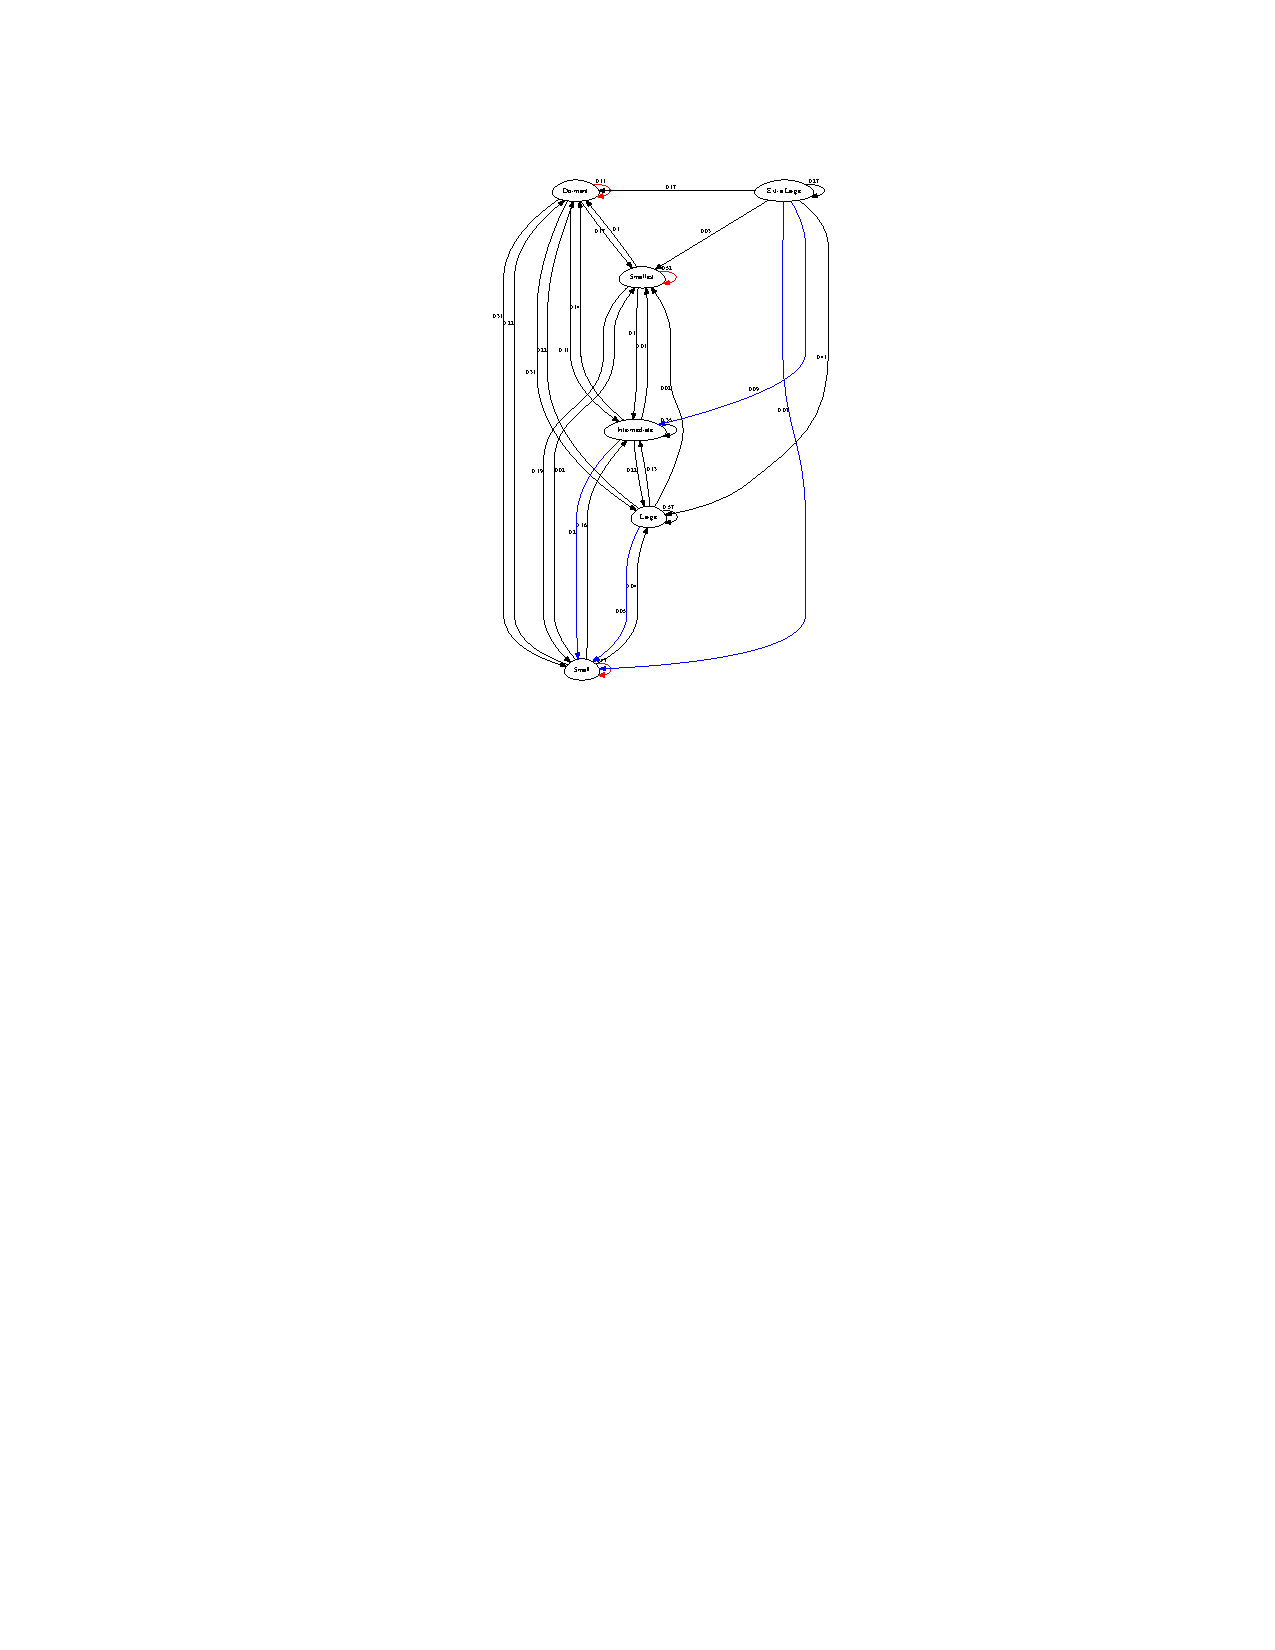
\includegraphics[keepaspectratio]{105-Transiciones_files/figure-pdf/Trans14-1.pdf}}

Los estudios sobre orquídeas que incorporan matrices de clonaje son poco
frecuentes, pero es fundamental considerar este proceso en los análisis
de dinámica poblacional. El clonaje puede tener un impacto significativo
tanto en la dinámica de las poblaciones como en la evolución de las
especies.

En este contexto, el clonaje se entiende como una forma de reproducción
asexual que puede modificar la estructura genética de la población y
afectar su capacidad de adaptación frente a cambios ambientales.

\begin{center}\rule{0.5\linewidth}{0.5pt}\end{center}

\subsection{Limitaciones de los métodos
tradicionales}\label{limitaciones-de-los-muxe9todos-tradicionales}

El uso de métodos tradicionales, ya sea mediante cálculos manuales o
utilizando la función \texttt{projection.matrix} del paquete popbio,
puede resultar problemático. Las dificultades surgen principalmente por
condiciones de muestreo, especialmente cuando el tamaño de muestra es
pequeño o cuando las transiciones son naturalmente raras (Tremblay
et~al., 2021; {Gascoigne et~al.}, 2023), situación común en especies
poco frecuentes.

En el capítulo \href{122-Impacto_de_Datos_sin_Sentido.qmd}{Impacto de
datos sin sentido biológico} se analizan los problemas que ocurren
cuando los datos carecen de coherencia biológica, cómo construir
matrices más confiables y cuándo es apropiado emplear el método
bayesiano en los análisis. Este enfoque permite resolver inconsistencias
y garantizar que las matrices sean más compatibles con la biología de la
especie estudiada, aumentando así la relevancia de los resultados.

Los autores recomiendan utilizar el \textbf{método bayesiano} para el
análisis de matrices de transición en la mayoría de los casos, excepto
cuando el tamaño de muestra es muy grande y ninguna transición es rara.
El método bayesiano es un enfoque estadístico que permite incorporar
información previa y ajustar los modelos a los datos observados. Este
enfoque es especialmente útil cuando se trabaja con datos escasos o
transiciones poco frecuentes. Aunque su implementación puede ser más
compleja, ofrece mayor flexibilidad y robustez, además de estimar la
confianza en los valores de transición y fecundidad.

\begin{tcolorbox}[enhanced jigsaw, arc=.35mm, bottomrule=.15mm, bottomtitle=1mm, breakable, colback=white, colbacktitle=quarto-callout-tip-color!10!white, colframe=quarto-callout-tip-color-frame, coltitle=black, left=2mm, leftrule=.75mm, opacityback=0, opacitybacktitle=0.6, rightrule=.15mm, title=\textcolor{quarto-callout-tip-color}{\faLightbulb}\hspace{0.5em}{Recomendación}, titlerule=0mm, toprule=.15mm, toptitle=1mm]

\textbf{Cambia al método bayesiano cuando los datos son escasos o las
transiciones son raras.} El método tradicional
(\texttt{projection.matrix()}) asume que las proporciones observadas
estiman bien las probabilidades de transición. Esta suposición se rompe
cuando el tamaño de muestra es pequeño o cuando alguna transición
ocurrió con frecuencia 0/n (común en transiciones raras). En esos casos,
el método bayesiano incorpora información a priori, evita probabilidades
exactamente 0 o 1, y produce intervalos de confianza explícitos. Ver el
capítulo \href{108-Bayesian_PPM.qmd}{Acercamiento bayesiano para
calcular transiciones y fecundidades}.

\end{tcolorbox}

\bookmarksetup{startatroot}

\chapter{Fecundidad}\label{MatricesF}

La fecundidad describe la contribución reproductiva de los individuos a
la población y constituye uno de los componentes clave de los modelos de
proyección poblacional. Este capítulo presenta los principios
conceptuales y prácticos necesarios para calcular la fecundidad y su
incorporación en matrices poblacionales estructuradas.

Por: Aucencia Emeterio-Lara y Raymond L. Tremblay

\section{Fecundidad y su representación en modelos matriciales de
población}\label{fecundidad-y-su-representaciuxf3n-en-modelos-matriciales-de-poblaciuxf3n}

La fecundidad representa el proceso mediante el cual los individuos
contribuyen nuevos reclutas a la población y es un componente esencial
de la dinámica poblacional. En los modelos matriciales, la fecundidad
suele integrarse como una combinación de producción reproductiva,
supervivencia temprana y transición hacia los estadios iniciales del
ciclo de vida.

En este capítulo se examinan los fundamentos para calcular la fecundidad
a partir de datos empíricos, destacando las decisiones conceptuales
necesarias para traducir observaciones biológicas, como floración,
producción de semillas o reclutamiento, en parámetros demográficos
coherentes. Se discuten las diferencias entre fecundidad potencial y
fecundidad realizada, así como las implicaciones de estas distinciones
para la interpretación de la dinámica poblacional.

\begin{tcolorbox}[enhanced jigsaw, arc=.35mm, bottomrule=.15mm, bottomtitle=1mm, breakable, colback=white, colbacktitle=quarto-callout-note-color!10!white, colframe=quarto-callout-note-color-frame, coltitle=black, left=2mm, leftrule=.75mm, opacityback=0, opacitybacktitle=0.6, rightrule=.15mm, title=\textcolor{quarto-callout-note-color}{\faInfo}\hspace{0.5em}{Nota}, titlerule=0mm, toprule=.15mm, toptitle=1mm]

\textbf{Fecundidad potencial vs realizada.}

\begin{itemize}
\tightlist
\item
  \textbf{Potencial:} lo que un individuo \emph{podría} producir en
  condiciones óptimas (p.~ej., número máximo de semillas si todas las
  flores son polinizadas).
\item
  \textbf{Realizada:} lo que un individuo efectivamente contribuye a la
  siguiente generación, descontando aborto, fallas en polinización,
  semillas inviables, fallas de germinación y mortalidad temprana.
\end{itemize}

Para modelos demográficos sólo es relevante la fecundidad
\textbf{realizada}, expresada en las mismas unidades que el primer
estadio del modelo.

\end{tcolorbox}

Asimismo, se analiza cómo la fecundidad se integra en la matriz de
proyección, generalmente a través de la submatriz \textbf{F}, y cómo su
parametrización influye en el crecimiento poblacional y en análisis
posteriores de sensibilidad y elasticidad. Este capítulo se diferencia
de los anteriores porque se centra en la cuantificación explícita de un
proceso demográfico específico, estableciendo el vínculo entre datos
reproductivos y modelos poblacionales utilizados para inferir patrones
de crecimiento y evaluar escenarios de manejo.

\subsubsection{Librerías de R requeridas para el siguiente
módulo}\label{libreruxedas-de-r-requeridas-para-el-siguiente-muxf3dulo-4}

\begin{Shaded}
\begin{Highlighting}[]
\FunctionTok{library}\NormalTok{(Rage)}
\FunctionTok{library}\NormalTok{(tidyverse)}
\end{Highlighting}
\end{Shaded}

\section{Introducción}\label{introducciuxf3n-2}

Toda población de organismos depende de la reproducción para su
crecimiento; sin ella, la población no puede aumentar. Por esta razón,
la reproducción es un proceso esencial para evaluar el crecimiento
poblacional y determinar si el reclutamiento es suficiente para sostener
dicho crecimiento. En el caso de las plantas, la reproducción puede ser
sexual o vegetativa. Cuando se considera el crecimiento vegetativo, es
necesario incorporar una matriz de clonación. Sin embargo, en este
capítulo nos enfocaremos únicamente en la reproducción sexual, que es la
más común en estudios de ecología de poblaciones.

La forma en que se obtiene e integra la reproducción en los modelos de
crecimiento poblacional es crucial, ya que su incorporación puede
influir en los resultados y en las conclusiones derivadas del modelo.
Por ello, comenzaremos describiendo errores frecuentes en el uso de
matrices de transición para calcular la fecundidad. La fecundidad
constituye una forma particular de transición demográfica, discutida en
el capítulo sobre transiciones poblacionales. La influencia de la
fecundidad sobre la dinámica poblacional se refleja directamente en la
tasa de crecimiento poblacional introducida en el capítulo sobre
crecimiento poblacional. La importancia relativa de la fecundidad frente
a otros procesos vitales se evalúa posteriormente mediante el análisis
de elasticidad poblacional.

El primer paso para calcular la fecundidad consiste en definir las
clases de edad o tamaño de los individuos. Estas clases agrupan
organismos con características similares en términos de edad o tamaño.
Por ejemplo, en una población de peces, las clases pueden ser:
juveniles, adultos jóvenes y adultos viejos; mientras que en plantas,
las clases suelen ser: plántulas, juveniles y adultos. Si la primera
etapa del modelo corresponde a ``plántula'', el reclutamiento debe
contabilizar las ``nuevas plántulas'' que ingresan a la población en
cada periodo. Es fundamental que la etapa reproductiva se mida en la
misma escala y periodo que las demás etapas.

Un error común es calcular la fecundidad usando el número de semillas
producidas cuando la primera etapa del modelo son plántulas. En este
caso, la fecundidad debe expresarse en términos de plántulas, no de
semillas. Para ello, es necesario convertir la cantidad de semillas en
plántulas mediante una tasa de germinación o de supervivencia.

\begin{tcolorbox}[enhanced jigsaw, arc=.35mm, bottomrule=.15mm, bottomtitle=1mm, breakable, colback=white, colbacktitle=quarto-callout-important-color!10!white, colframe=quarto-callout-important-color-frame, coltitle=black, left=2mm, leftrule=.75mm, opacityback=0, opacitybacktitle=0.6, rightrule=.15mm, title=\textcolor{quarto-callout-important-color}{\faExclamation}\hspace{0.5em}{Importante}, titlerule=0mm, toprule=.15mm, toptitle=1mm]

\textbf{La fecundidad debe expresarse en las mismas unidades que el
primer estadio del modelo.} Si la primera etapa es ``plántula'', la
entrada de fecundidad cuenta nuevas plántulas por individuo reproductor,
no semillas. Mezclar unidades (e.g., poner ``número de semillas'' en una
matriz cuya primera etapa son plántulas) introduce un error sistemático
que infla λ por órdenes de magnitud. Cuando sólo se conoce la producción
de semillas, hay que multiplicarla por las tasas de germinación y
supervivencia hasta plántula antes de incorporarla a la matriz.

\end{tcolorbox}

\section{Estimación de la fecundidad a partir de
datos}\label{estimaciuxf3n-de-la-fecundidad-a-partir-de-datos}

A continuación se presentan los métodos y cálculos utilizados para
estimar la fecundidad y su incorporación en matrices de proyección
poblacional.

\section{La fecundidad de las orquídeas en la demografía
poblacional}\label{la-fecundidad-de-las-orquuxeddeas-en-la-demografuxeda-poblacional}

La fecundidad en orquídeas se refiere a la capacidad reproductiva
efectiva de una población, evaluada a través de una serie de eventos:
producción de flores, éxito en la polinización, formación de frutos,
germinación de semillas y establecimiento de plántulas. En consecuencia,
la fecundidad constituye un conjunto de procesos que determinan la
viabilidad poblacional a largo plazo. Aunque puede parecer un mecanismo
sencillo, en realidad es complejo, ya que depende de múltiples factores
como la disponibilidad de recursos, competencia entre individuos,
depredación y enfermedades.

El proceso inicia con la producción de flores, lo que implica una
inversión significativa de nutrientes y agua acumulados por la planta.
Además, las flores desarrollan atributos específicos para maximizar la
probabilidad de polinización, tales como color, aroma, néctar y polen.
Estos rasgos, sin embargo, son costosos en términos energéticos, por lo
que su expresión debe ser cuidadosamente optimizada. En algunos casos,
los costos reproductivos son tan elevados que pueden comprometer la
supervivencia de la planta.

Diversos estudios ilustran este fenómeno. Por ejemplo, en la orquídea
\emph{Comparettia falcata} (Meléndez-Ackerman, Ackerman \&
Rodriguez-Robles, 2000), la polinización manual mostró una correlación
positiva entre el número de flores producidas y el porcentaje de frutos
abortados. En \emph{Spiranthes spiralis}, un año con alta producción
floral se tradujo en más del 80\% de individuos en estado vegetativo al
año siguiente (Willems \& Dorland, 2000). De manera similar, en la
orquídea perenne \emph{Cypripedium acaule} se observó una reducción en
la probabilidad de florecer y en el tamaño foliar en la temporada
posterior (Primack \& Stacy, 1998). Otro caso se reportó en
\emph{Encyclia krugii}, donde el incremento en la producción de frutos
se compensó en la siguiente temporada con menor crecimiento vegetativo
(reducción en tamaño de hojas, número de flores, inflorescencias y mayor
aborto de frutos) (Ackerman, 1989).

Estos hallazgos sugieren que cada ciclo reproductivo requiere un periodo
de recuperación para que la planta acumule los nutrientes necesarios
para la siguiente temporada. Por lo tanto, un alto índice reproductivo
---y el consecuente costo energético--- puede representar una desventaja
significativa, especialmente en especies con reservas limitadas.

\section{La polinización en las
orquídeas}\label{la-polinizaciuxf3n-en-las-orquuxeddeas}

La familia \emph{Orchidaceae} exhibe una notable diversidad en sus
sistemas reproductivos, incluyendo especies autógamas y alógamas
(Willmer, 2011; Bateman, 2020). Aunque muchas orquídeas presentan
barreras físicas o genéticas que limitan la autopolinización (por
ejemplo, el rostelo o la incompatibilidad genética), se ha documentado
que varias especies pueden utilizar su propio polen para producir frutos
y semillas viables (Ackerman et~al., 2023). De hecho, Catling reporta al
menos 350 especies en las que alguna población se autopoliniza (Catling,
1990). Se estima que aproximadamente el 31\% de las especies de
orquídeas producen frutos mediante autopolinización (Evans \& Jacquemyn,
2020), siendo esta estrategia más frecuente en especies con distribución
geográfica restringida o en ambientes con escasez de polinizadores
(Suetsugu, 2015).

Es importante destacar que la autopolinización no implica necesariamente
autogamia estricta; la mayoría de las orquídeas presentan grados
variables de autogamia facultativa. Este tipo de autopolinización se ha
observado bajo condiciones de estrés abiótico o disturbios
antropogénicos (Talalaj \& Skierczynski, 2015; Tałałaj et~al., 2017).
Por ejemplo, las flores del género \emph{Epipactis} muestran
adaptaciones morfológicas que facilitan la autopolinización para
asegurar la producción de semillas. Si bien la autogamia garantiza la
formación de frutos, estos suelen ser más pequeños y contener menos
semillas, con menor viabilidad (semillas sin embrión, embriones
inviables, protocormos albinos) (Tremblay et~al., 2005; Paiva Neto
et~al., 2022). Este fenómeno se asocia con la autocompatibilidad
genética, documentada en más de 750 especies de orquídeas, incluyendo
géneros como \emph{Chondrorhyncha}, \emph{Coelogyne}, \emph{Dendrobium},
\emph{Lycaste}, \emph{Notylia} y \emph{Oncidium} (Johnson \& Edwards,
2000; Tremblay et~al., 2005; Barreda-Castillo et~al., 2024).

Por otro lado, la polinización cruzada incrementa el éxito reproductivo
al introducir diversidad genética y superar mecanismos de
auto-incompatibilidad (Zhang et~al., 2021). Aunque las especies
autocompatibles suelen producir más frutos (Caballero-Villalobos et~al.,
2017), muchas orquídeas dependen exclusivamente de la polinización
cruzada (Zhang et~al., 2021). Por ejemplo, en la subfamilia
\emph{Epidendroideae} existe un alto número de especies autoestériles,
mientras que en \emph{Vanilloideae} y \emph{Cypripedioideae} se observa
producción de frutos por autopolinización, a pesar de que su morfología
floral sugiere polinización cruzada (Suetsugu \& Fukushima, 2014; {Lopes
et~al.}, 2022).

Algunas especies presentan autopolinización estricta mediante flores
cleistógamas, que nunca se abren pero producen frutos fértiles, como en
\emph{Lepanthes dodiana}. Esta estrategia es común en plantas
colonizadoras o adaptadas a ambientes extremos, donde la ausencia de
polinizadores o individuos cercanos limita la polinización cruzada
(Barreda-Castillo et~al., 2024). La autogamia, además, requiere menos
inversión energética al no producir recompensas florales (Eckert \&
Herlihy, 2004), similar a las especies que emplean polinización por
engaño, donde la ausencia de recompensas se traduce en menor éxito
reproductivo (Golubov \& Mandujano, 2009).

Se estima que aproximadamente el 65\% de las especies de
\emph{Orchidaceae} ofrecen algún tipo de recompensa floral (Llabrés
Fernández, 2015). El néctar constituye la recompensa más común para
atraer polinizadores (Neiland \& Wilcock, 1998); sin embargo, su
producción pudiese implicar un elevado costo energético para la planta,
lo que puede limitar el desarrollo de otras estructuras. Ante esta
restricción, muchas orquídeas han evolucionado mecanismos de
polinización por engaño, estrategia presente en cerca de un tercio de
las especies (entre 6,000 y 8,000) (Dafni, 1983; Ackerman, 1989;
Tremblay et~al., 2005; Case \& Bradford, 2009). Estas especies no
ofrecen recompensa alguna, lo que reduce el gasto energético. La
ausencia de recompensas permite a las orquídeas con polinización por
engaño invertir recursos en otras características, como mayor número de
flores, incremento en la altura de la planta y en el tamaño de la
inflorescencia (Henneresse, Wesselingh \& Tyteca, 2017; Scopece et~al.,
2017), rasgos que aumentan la atracción visual y la frecuencia de
visitas de polinizadores (Peakall, 1989; Burd, 1995; Aragón \& Ackerman,
2004; Grindeland, Sletvold \& Ims, 2005; Li et~al., 2011; Sletvold \&
Ågren, 2011). Tanto la autogamia como la polinización por engaño
requieren menor inversión energética al no producir recompensas (Eckert
\& Herlihy, 2004); sin embargo, esta estrategia suele traducirse en
menor éxito reproductivo. De hecho, se ha reportado que las orquídeas
que emplean polinización por engaño producen, en promedio, solo la mitad
de frutos en comparación con aquellas que ofrecen recompensas (Johnson
\& Bond, 1997; Neiland \& Wilcock, 1998; Tremblay et~al., 2005;
Jersáková, Johnson \& Kindlmann, 2006).

\section{Producción de frutos en
orquídeas}\label{producciuxf3n-de-frutos-en-orquuxeddeas}

En los análisis de demografía poblacional, la fecundidad se ha estimado
a distintos niveles: número de flores, frutos, semillas o plántulas.
Algunos estudios la calculan considerando la cantidad de flores
producidas por planta en relación con el número de individuos en la
población, mientras que otros proponen que la producción de frutos es el
indicador más preciso del éxito reproductivo (Proctor \& Harder, 1994).

Por ejemplo, en \emph{Dracula chimaera} la fecundidad se determinó
calculando la probabilidad de que una planta con flor desarrollara
fruto, es decir, el número de frutos presentes en cada etapa dividido
entre el total de plantas de esa misma etapa. Sin embargo, es importante
subrayar que la producción de frutos no garantiza la calidad de las
semillas o la presencia de semillas; por ejemplo, en la especie
\emph{Psychilis krugii} en Puerto Rico, la autopolinización resulta en
la producción de un fruto pero las semillas están sin embrión. Además,
hay muchos factores que influyen directamente en la germinación y, a
largo plazo, en el establecimiento efectivo de nuevas plántulas.

\section{Viabilidad de las semillas}\label{viabilidad-de-las-semillas}

El número de semillas por fruto en las orquídeas puede variar desde
miles hasta millones; sin embargo, no todas son viables. Es ampliamente
reconocido que una gran proporción corresponde a semillas vacías (sin
embrión), mientras que otras presentan embriones no funcionales. Esto
indica que no todas las semillas producidas tienen la capacidad de
originar un nuevo individuo. Por esta razón, algunos estudios han
incorporado la viabilidad de las semillas como un nivel adicional para
estimar la fecundidad, tal como se realizó en \emph{Laelia autumnalis}
(Emeterio-Lara; comunicación personal).

\section{Germinación}\label{germinaciuxf3n}

Aunque una planta puede producir una gran cantidad de semillas viables,
tras la dispersión estas enfrentan múltiples factores que limitan su
éxito. Las condiciones abióticas ---como temperatura, luz y humedad---,
junto con factores bióticos, como las características del forófito, la
disponibilidad de hongos endófitos y la presión de herbívoros o
depredadores de semillas y plántulas, influyen tanto en la micorrización
como en la germinación y el establecimiento de nuevas plántulas
(Dressler, 1993).

Estos elementos definen micrositios específicos para la germinación, que
pueden incluir fisuras en la corteza de un árbol, mechones de musgo,
superficies de raíces vivas o acumulaciones de humus (Rasmussen et~al.,
2015). A medida que las semillas atraviesan las distintas etapas de
germinación, desde la imbibición hasta el desarrollo de plántulas con
dos hojas (Arditti, 1967), la mortalidad se mantiene en niveles muy
altos. Por ejemplo, Batty et al. (Batty et~al., 2001) estimaron que, en
\emph{Caladenia arenicola}, de aproximadamente 34,500 semillas, menos
del 1\% alcanzó la etapa de plántula capaz de sobrevivir a la primera
sequía estival.

\section{Reclutamiento}\label{reclutamiento}

El reclutamiento se define como el número de plántulas que logran
establecerse en el forófito y poseen el potencial de sobrevivir para
avanzar a la siguiente etapa demográfica (juvenil). Las orquídeas
presentan tasas de reclutamiento particularmente bajas (Larson \&
Batson, 1978; Zotz, 1998; Winkler \& Hietz, 2001; Garcı́a-Soriano, 2003),
debido a factores como la susceptibilidad al estrés hídrico durante la
estación seca (Benzing, 1981; Hernández-Apolinar, 1992; Larson, 1992;
Hietz, 1997; Tremblay, 1997a; Zotz, 1998; Mondragón, 2000;
Garcı́a-Soriano, 2003), enfermedades y depredación. Por ejemplo, en
\emph{Erycina crista-galli} un individuo adulto produce en promedio
0.033 plántulas/año, mientras que en \emph{Guarianthe aurantiaca} un
individuo reproductivo genera menos de un nuevo individuo por año.

En los modelos demográficos, alcanzar esta fase es crucial, ya que
representa el valor neto de fecundidad: el número de nuevos individuos
que conformarán la siguiente generación en una población natural. Sin
embargo, estimar la fecundidad hasta la etapa de plántula es uno de los
mayores retos, principalmente por la dificultad de asegurar la identidad
de la especie. Un aspecto clave es la proximidad a la planta madre, dado
que, aunque el viento favorece la dispersión a larga distancia, la
mayoría de las semillas se depositan cerca de ella (Chung, Nason \&
Chung, 2004; Trapnell, Hamrick \& Nason, 2004; Jersáková \& Malinová,
2007).

A pesar de estas limitaciones, existen estudios que han registrado
plántulas sobrevivientes tras un periodo (generalmente un año). Ejemplos
incluyen \emph{Brassavola cucullata} (Ackerman et~al., 2020) y \emph{E.
crista-galli} ({Maldonado Flores et~al.}, 2006), donde la fecundidad se
estimó dividiendo el número de nuevos reclutas observados en campo entre
el número máximo de frutos reportados durante el periodo de estudio. En
otros casos, como \emph{Guarianthe aurantiaca}, se calculó comparando
los reclutamientos entre años consecutivos (Mondragón, 2009). Estos
datos proporcionan estimaciones más precisas para proyectar la dinámica
poblacional y diseñar estrategias de conservación.

\begin{tcolorbox}[enhanced jigsaw, arc=.35mm, bottomrule=.15mm, bottomtitle=1mm, breakable, colback=white, colbacktitle=quarto-callout-warning-color!10!white, colframe=quarto-callout-warning-color-frame, coltitle=black, left=2mm, leftrule=.75mm, opacityback=0, opacitybacktitle=0.6, rightrule=.15mm, title=\textcolor{quarto-callout-warning-color}{\faExclamationTriangle}\hspace{0.5em}{Advertencia}, titlerule=0mm, toprule=.15mm, toptitle=1mm]

\textbf{Una flor no es un fruto, un fruto no es una semilla viable, una
semilla no es una plántula.} La fecundidad efectiva en orquídeas resulta
de una cadena de filtros sucesivos: producción floral → polinización
exitosa → cuajado de fruto → producción de semillas con embrión →
germinación → establecimiento. En cada paso, la mortalidad puede ser muy
alta (p.~ej., en \emph{Caladenia arenicola} menos del 1\% de las
semillas llega a plántula). Asumir que un fruto observado equivale a una
plántula establecida sobreestima la fecundidad realizada en varios
órdenes de magnitud.

\end{tcolorbox}

\begin{figure}[H]

{\centering \pandocbounded{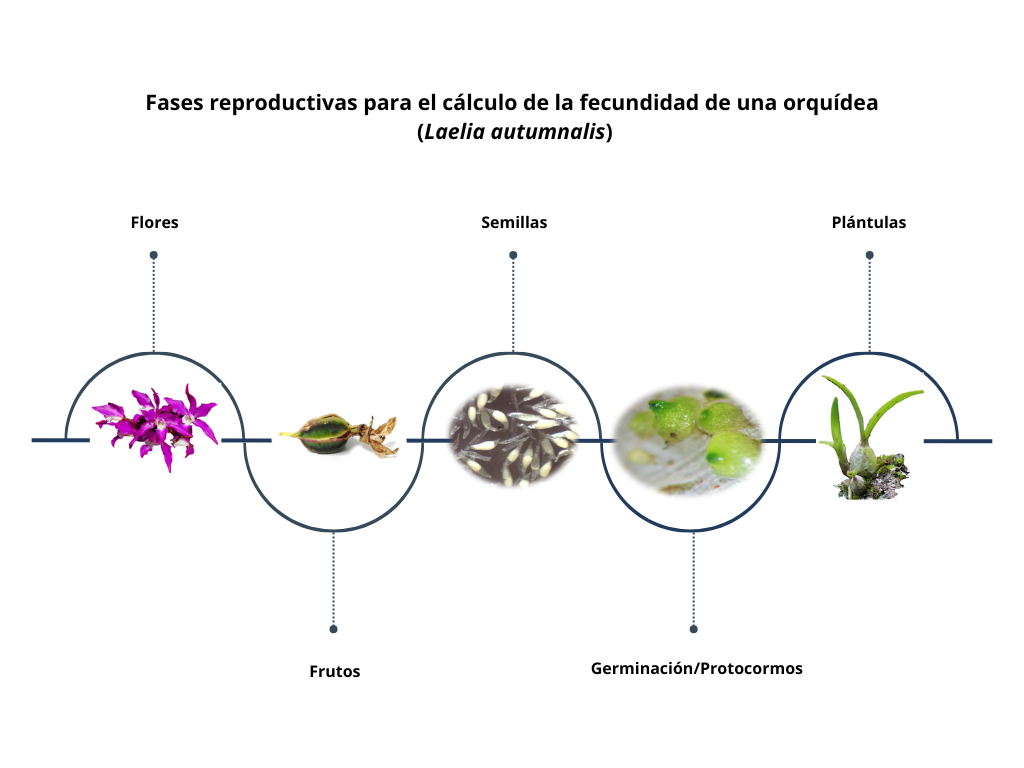
\includegraphics[keepaspectratio,alt={Diagrama esquemático del proceso de fecundidad en orquídeas, con la cadena de eventos desde la flor hasta el establecimiento de la plántula}]{images/Diagrama_fecundidad.png}}

}

\caption{Diagrama del proceso de fecundidad en orquídeas, mostrando la
cadena de filtros sucesivos: producción floral, polinización exitosa,
cuajado de fruto, producción de semillas con embrión, germinación y
establecimiento de plántulas}

\end{figure}%

\begin{center}\rule{0.5\linewidth}{0.5pt}\end{center}

Tabla de algunos ejemplos de fecundidad en orquídeas, donde se muestra
la especie, el índice de fecundidad y la referencia del estudio.

{\def\LTcaptype{none} % do not increment counter
\begin{longtable}[]{@{}
  >{\raggedright\arraybackslash}p{(\linewidth - 4\tabcolsep) * \real{0.3333}}
  >{\raggedright\arraybackslash}p{(\linewidth - 4\tabcolsep) * \real{0.3333}}
  >{\raggedright\arraybackslash}p{(\linewidth - 4\tabcolsep) * \real{0.3333}}@{}}
\toprule\noalign{}
\begin{minipage}[b]{\linewidth}\raggedright
Especie
\end{minipage} & \begin{minipage}[b]{\linewidth}\raggedright
Indice de Fecundidad
\end{minipage} & \begin{minipage}[b]{\linewidth}\raggedright
Referencia
\end{minipage} \\
\midrule\noalign{}
\endhead
\bottomrule\noalign{}
\endlastfoot
\emph{Lepanthes eltoroensis} & Cantidad de Plántulas / Adultos
reproductivos & Tremblay \& Hutchings (2003) \\
\emph{Erycina crista-galli} & 0.033 plántulas/año & Maldonado Flores
(2005) \\
\emph{Encyclia tampensis} & 0.1 plántulas/fruto & Larson (1992) \\
\emph{Guarianthe aurantiaca} & \textless1 plántula/año & Mondragón
(2009) \\
\end{longtable}
}

\section{Tiempo de inversión para alcanzar la fase
reproductiva}\label{tiempo-de-inversiuxf3n-para-alcanzar-la-fase-reproductiva}

Los estudios disponibles indican que las orquídeas presentan un
crecimiento lento, requiriendo entre 8 y 19 años para alcanzar la
madurez reproductiva (Hernández-Apolinar, 1992; Larson, 1992; Zotz,
1995, 1998). Sin embargo, existen excepciones, como las orquídeas
miniatura o de ramilla (principalmente \emph{Pleurothalliinae}), que
pueden madurar en uno o pocos años (1-3 años) (Chase, 1987), en
contraste con los 8-19 años requeridos por las especies de mayor tamaño.

Para estimar el crecimiento y la edad reproductiva en \emph{Lycaste
aromatica}, se ha utilizado la producción regular de pseudobulbos, los
cuales permanecen varios años en la planta. Con base en este patrón, se
predice que \emph{Encyclia tampensis} alcanza la floración
aproximadamente a los 15 años. No obstante, bajo condiciones controladas
de cultivo, la fase de pre-bulbo puede durar entre 0.5 y 2 años, y la
primera floración ocurrir en tan solo 5 a 6 años (H. Lutero,
comunicación personal).

\begin{figure}[H]

{\centering \pandocbounded{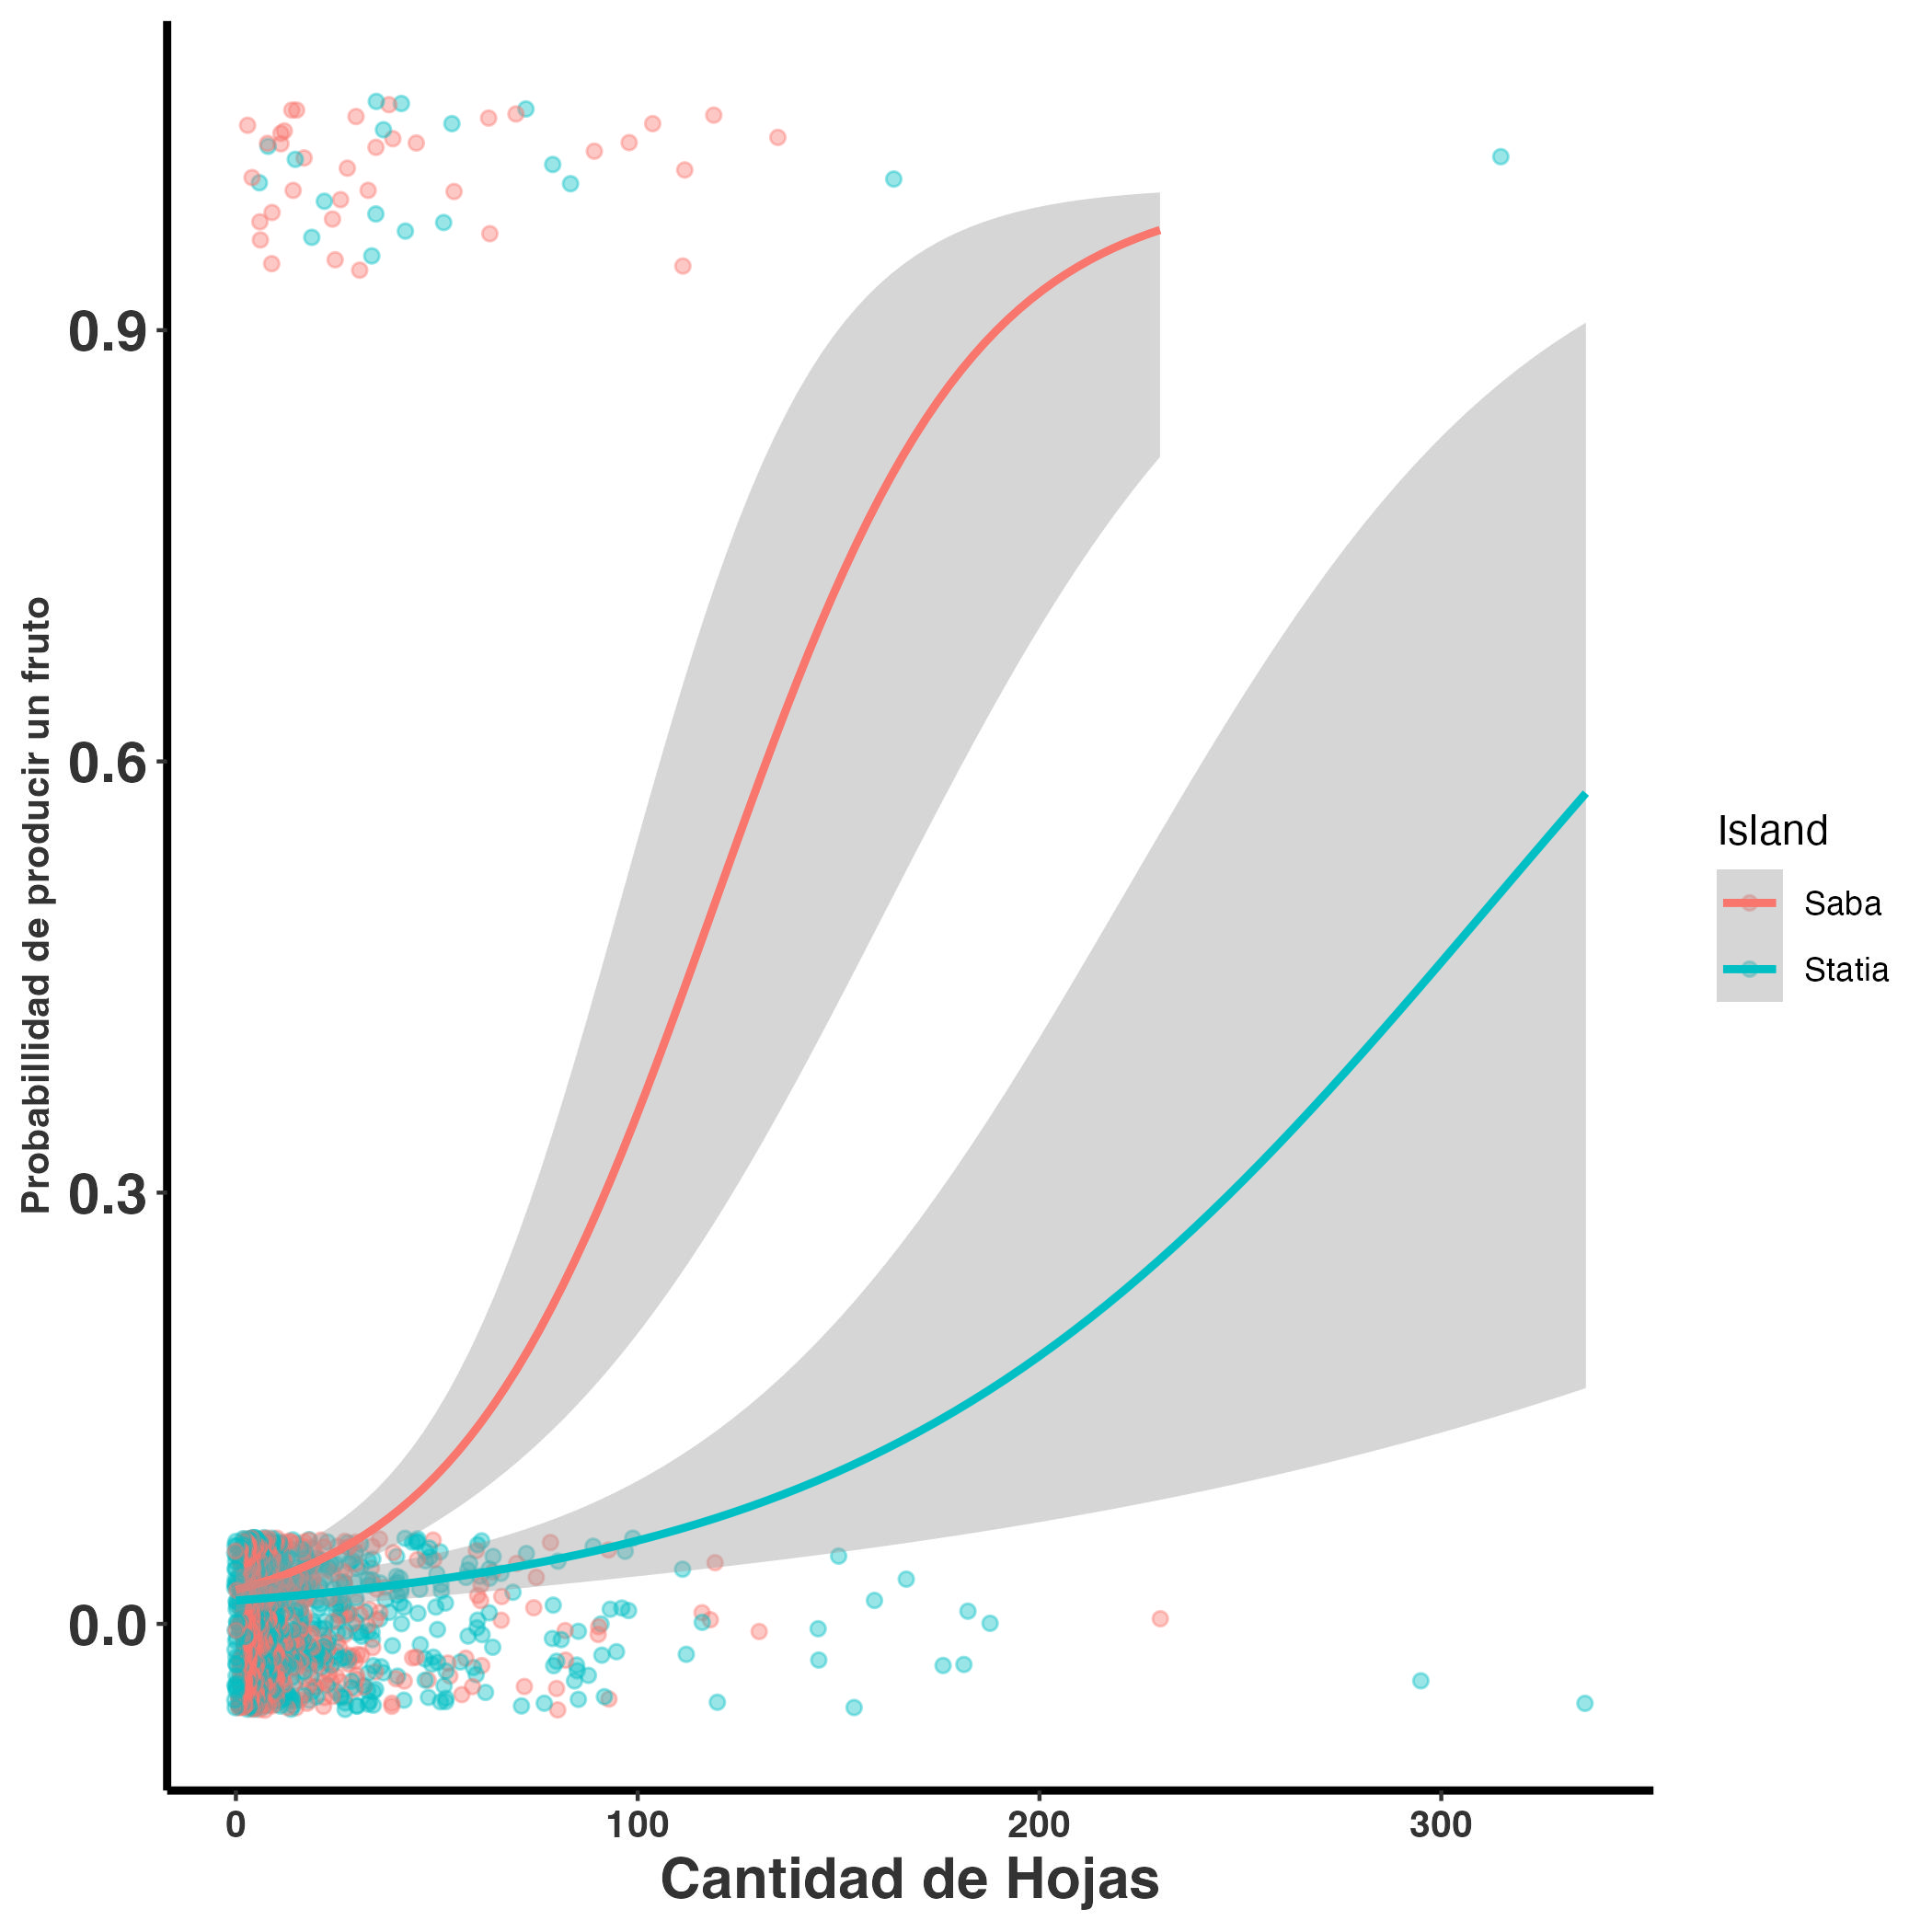
\includegraphics[keepaspectratio,alt={Gráfica de la probabilidad de floración como función del número de hojas en Brassavola cucullata, con curvas separadas para las poblaciones de Saba y San Eustaquio}]{images/Cant_Hojas_Prob_Fr_Brassavola.jpg}}

}

\caption{Relación entre la cantidad de hojas y la probabilidad de
floración en \emph{Brassavola cucullata} en las islas Saba y San
Eustaquio}

\end{figure}%

Un caso interesante se observa en \emph{Brassavola cucullata}, una
especie rupícola y epífita de las Antillas Menores. En esta orquídea,
los pseudobulbos presentan hojas lanceoladas, y la probabilidad de
floración no depende de la longitud de las hojas, sino de la cantidad de
hojas por individuo. De hecho, el número estimado de hojas constituye un
buen predictor de la capacidad de una planta para producir flores,
aunque se han registrado diferencias en esta relación entre las
poblaciones de las islas Saba y San Eustaquio.

\section{Ejemplo de cálculo de fecundidad basado en
semillas}\label{ejemplo-de-cuxe1lculo-de-fecundidad-basado-en-semillas}

En este ejemplo, la primera fila de la matriz representa la fecundidad
de la población en la posición (3,1) (columna, fila), correspondiente al
número promedio de semillas producidas por un individuo adulto. Sin
embargo, la fecundidad en modelos demográficos debe expresarse en
términos de plántulas, no de semillas. Por ello, es necesario convertir
la cantidad de semillas producidas en plántulas mediante una tasa de
germinación o una tasa de supervivencia hasta la etapa de plántula. De
lo contrario, el cálculo presentará un sesgo, ya que se estaría
estimando fecundidad con base en semillas, sin considerar su capacidad
real de generar nuevos individuos.

\begin{Shaded}
\begin{Highlighting}[]
\NormalTok{matA\_sem }\OtherTok{\textless{}{-}} \FunctionTok{rbind}\NormalTok{(}
  \FunctionTok{c}\NormalTok{(}\FloatTok{0.0}\NormalTok{, }\FloatTok{0.0}\NormalTok{, }\DecValTok{1000}\NormalTok{), }\CommentTok{\#  fecundidad 1000 semillas en promedio por adulto}
  \FunctionTok{c}\NormalTok{(}\FloatTok{0.5}\NormalTok{, }\FloatTok{0.0}\NormalTok{, }\FloatTok{0.0}\NormalTok{),}
  \FunctionTok{c}\NormalTok{(}\FloatTok{0.0}\NormalTok{, }\FloatTok{0.4}\NormalTok{, }\FloatTok{0.0}\NormalTok{)}
\NormalTok{)}
\end{Highlighting}
\end{Shaded}

Visualizamos el ciclo de vida de la población con la función
\texttt{plot\_life\_cycle()} de la librería \texttt{Rage}:

\begin{Shaded}
\begin{Highlighting}[]
\NormalTok{etapas }\OtherTok{\textless{}{-}} \FunctionTok{c}\NormalTok{(}\StringTok{"plántula"}\NormalTok{, }\StringTok{"juvenil"}\NormalTok{, }\StringTok{"adulto"}\NormalTok{)}
 
 \FunctionTok{plot\_life\_cycle}\NormalTok{(matA\_sem, }\AttributeTok{stages=}\NormalTok{etapas, }\AttributeTok{fontsize =} \DecValTok{5}\NormalTok{)}
\end{Highlighting}
\end{Shaded}

\pandocbounded{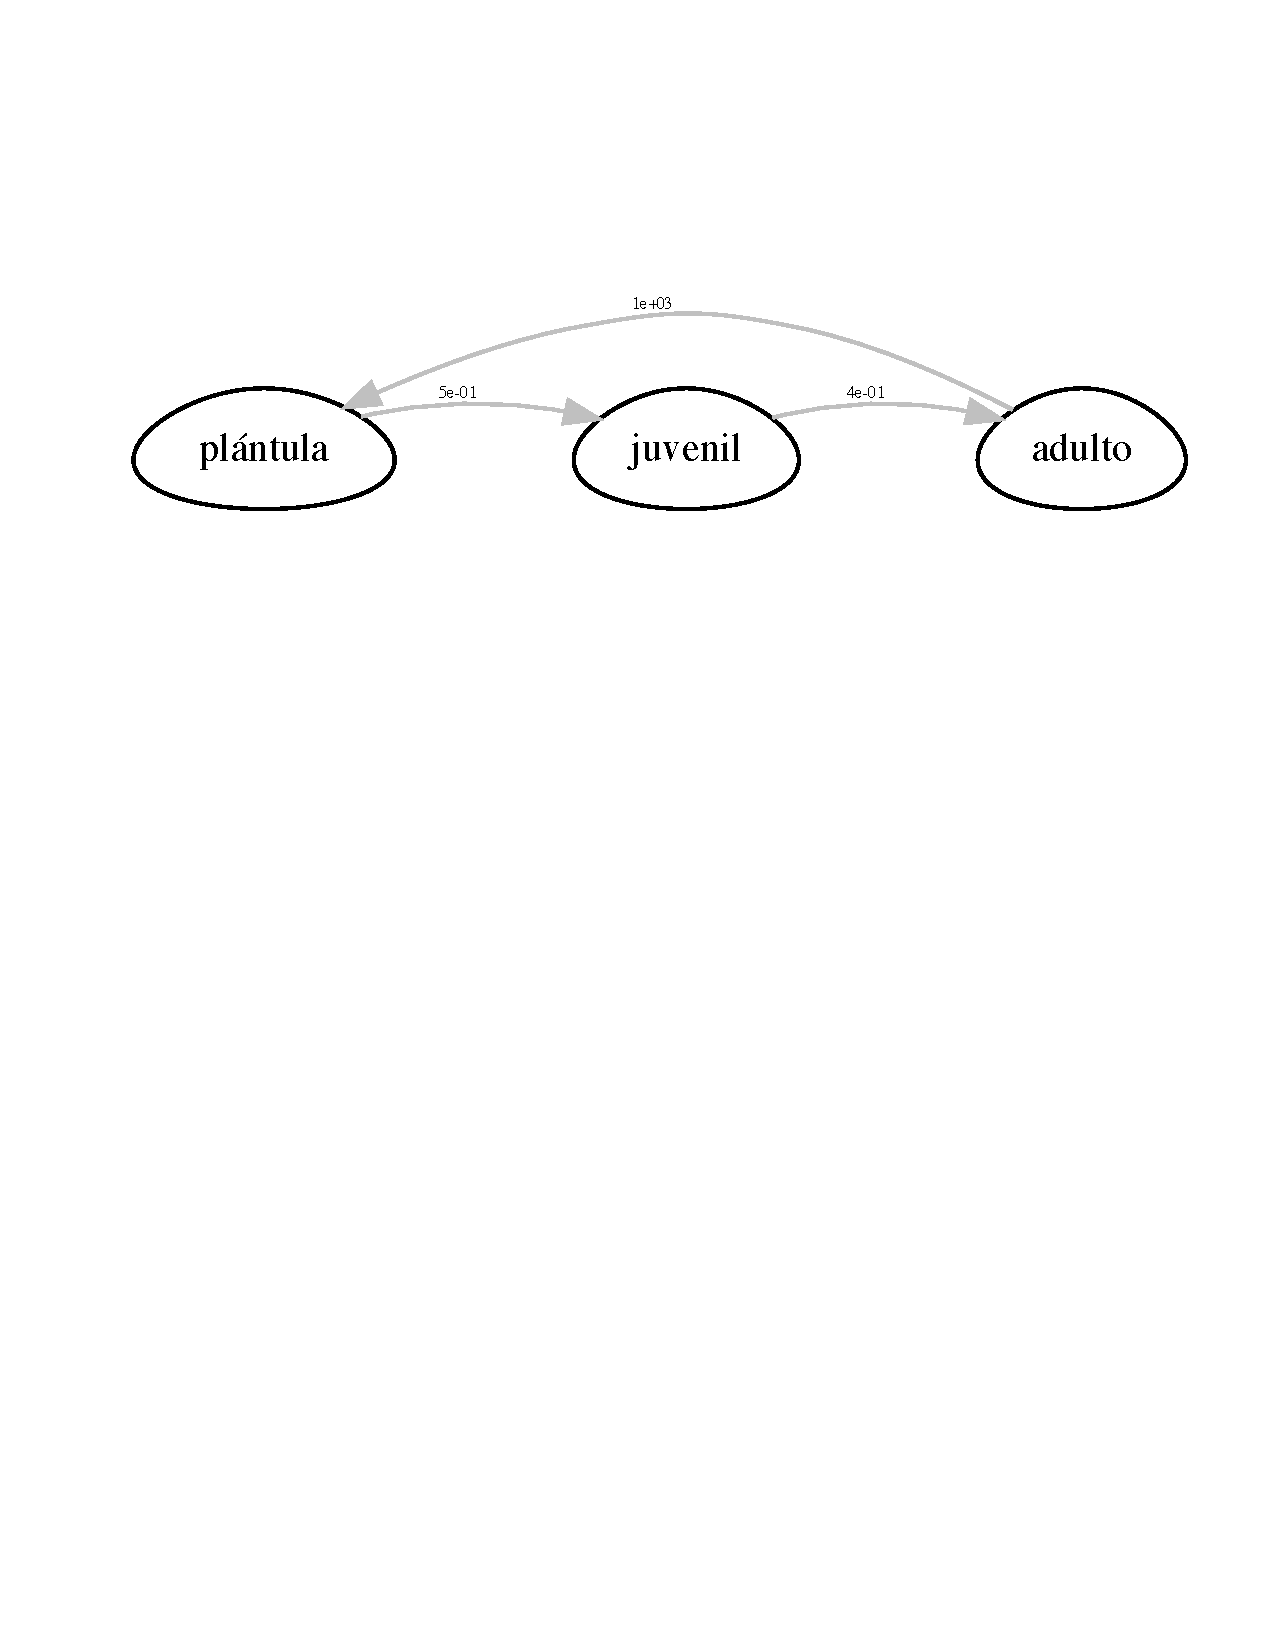
\includegraphics[keepaspectratio]{106-calcular_fecundidad_files/figure-pdf/unnamed-chunk-2-1.pdf}}

\begin{center}\rule{0.5\linewidth}{0.5pt}\end{center}

\section{Ejemplo de cálculo de fecundidad de semillas a
plántulas}\label{ejemplo-de-cuxe1lculo-de-fecundidad-de-semillas-a-pluxe1ntulas}

Una alternativa para estimar la fecundidad en términos demográficos
consiste en calcular el número de nuevas plántulas que se incorporarán
en el siguiente periodo, utilizando una tasa de germinación y una tasa
de supervivencia hasta la etapa de plántula.

Por ejemplo, si:

\begin{itemize}
\tightlist
\item
  la tasa de germinación es 50\%,
\item
  la tasa de supervivencia de plántulas es 20\%,
\item
  y existen 75 adultos reproductivos,
\end{itemize}

entonces la fecundidad en términos de plántulas se calcula como:

\[\text{Fecundidad} = \frac{(1000 \times 0.5 \times 0.2)}{75} = 1.33\]

Esto significa que, en promedio, cada adulto contribuiría con 1.33
plántulas al siguiente periodo.

Por consecuencia la matriz cambia a:

\begin{Shaded}
\begin{Highlighting}[]
\NormalTok{matA\_pl }\OtherTok{\textless{}{-}} \FunctionTok{rbind}\NormalTok{(}
  \FunctionTok{c}\NormalTok{(}\FloatTok{0.0}\NormalTok{, }\FloatTok{0.0}\NormalTok{, }\FloatTok{1.333}\NormalTok{), }
  \FunctionTok{c}\NormalTok{(}\FloatTok{0.5}\NormalTok{, }\FloatTok{0.0}\NormalTok{, }\FloatTok{0.0}\NormalTok{),}
  \FunctionTok{c}\NormalTok{(}\FloatTok{0.0}\NormalTok{, }\FloatTok{0.4}\NormalTok{, }\FloatTok{0.0}\NormalTok{)}
\NormalTok{)}

\NormalTok{etapas }\OtherTok{\textless{}{-}} \FunctionTok{c}\NormalTok{(}\StringTok{"plántula"}\NormalTok{, }\StringTok{"juvenil"}\NormalTok{, }\StringTok{"adulto"}\NormalTok{)}

\FunctionTok{plot\_life\_cycle}\NormalTok{(matA\_pl, }\AttributeTok{stages =}\NormalTok{ etapas, }\AttributeTok{fontsize =} \DecValTok{5}\NormalTok{)}
\end{Highlighting}
\end{Shaded}

\pandocbounded{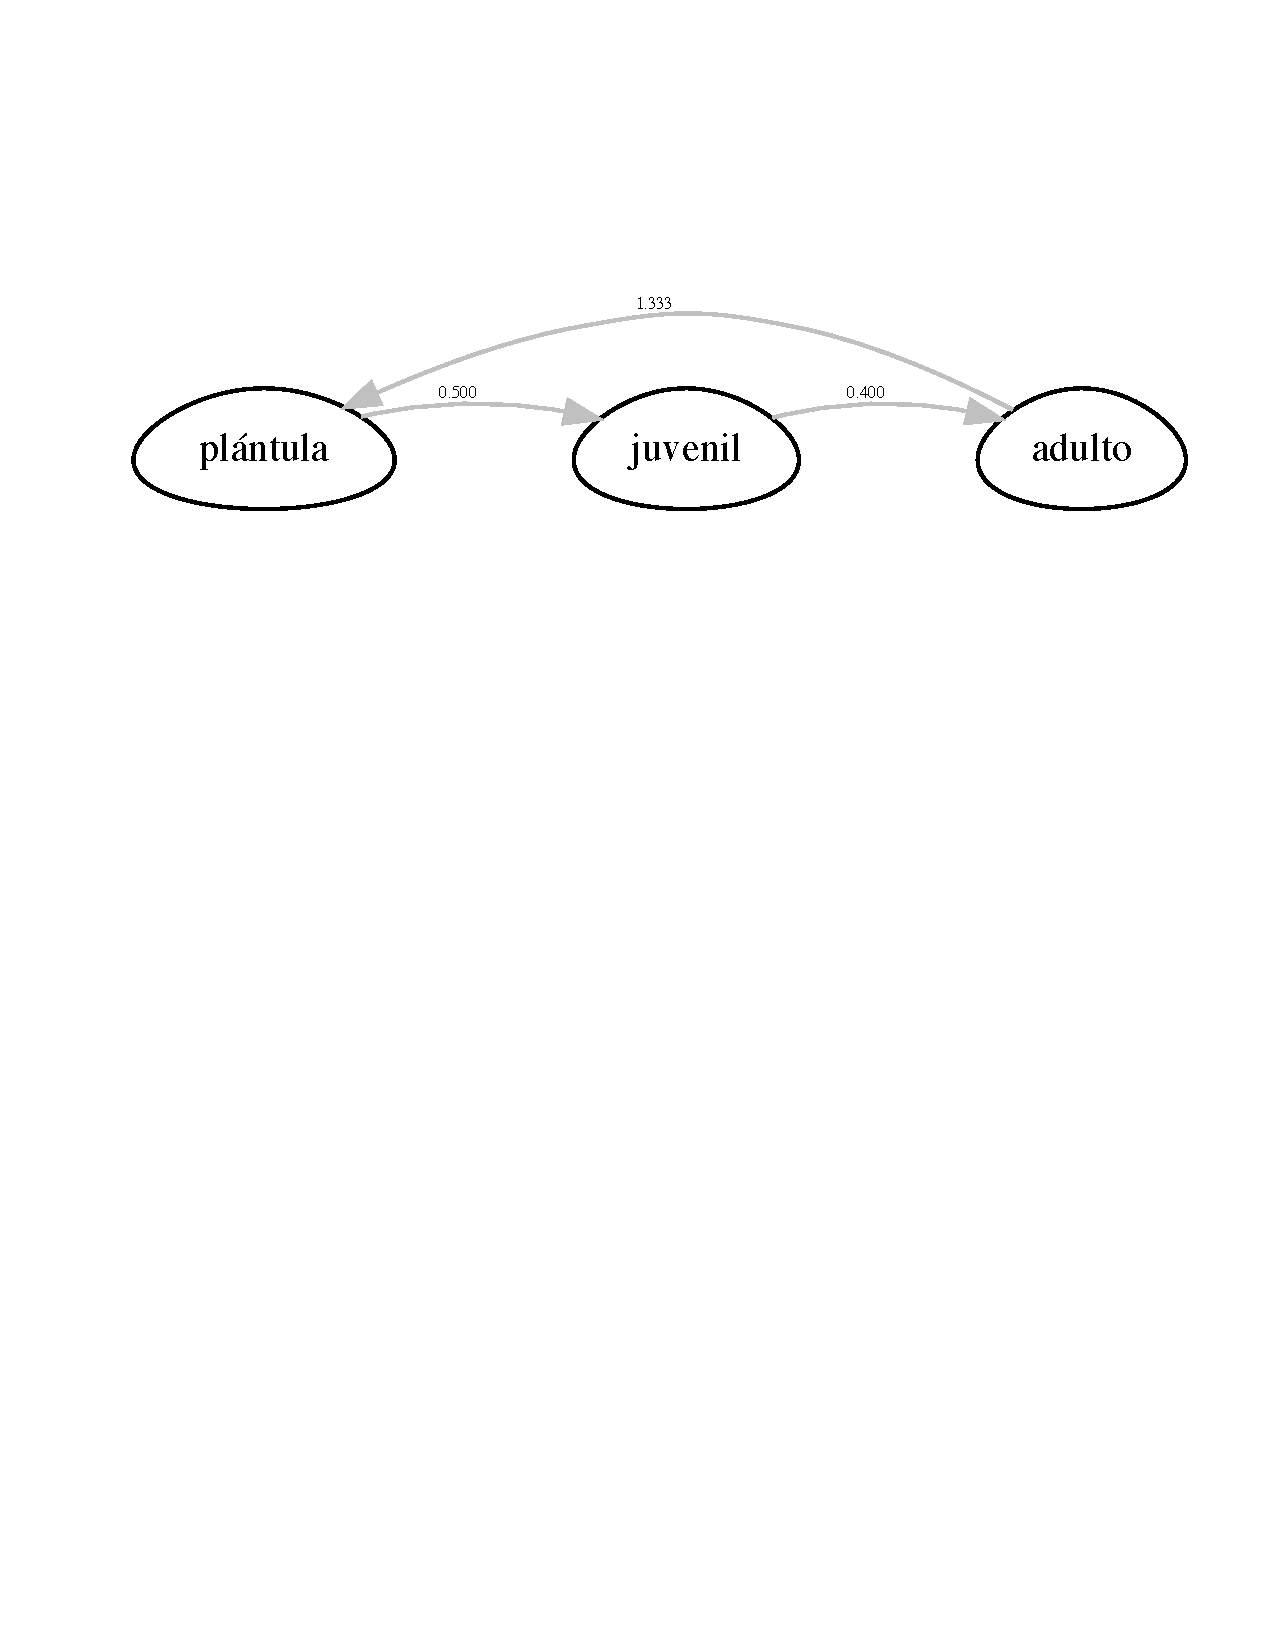
\includegraphics[keepaspectratio]{106-calcular_fecundidad_files/figure-pdf/unnamed-chunk-3-1.pdf}}

\begin{center}\rule{0.5\linewidth}{0.5pt}\end{center}

\section{Fecundidad en términos de
plántulas}\label{fecundidad-en-tuxe9rminos-de-pluxe1ntulas}

Otra alternativa consiste en calcular la fecundidad directamente en
función del reclutamiento observado, utilizando el número de plántulas
establecidas en el periodo siguiente. Este método es útil cuando no se
dispone de información sobre la producción de semillas ni sobre sus
tasas de germinación y supervivencia.

La estimación se obtiene dividiendo el número total de plántulas
registradas en el periodo \(t_2\) entre el número de adultos presentes
en el periodo anterior \(t_1\). Por ejemplo, si en \(t_2\) se
contabilizan 50 nuevas plántulas y en \(t_1\) había 100 adultos, la
fecundidad sería:

\[\text{Fecundidad} = \frac{50}{100} = 0.5\]

Esto indica que, en promedio, cada adulto contribuyó con 0.5 plántulas a
la siguiente generación.

\begin{Shaded}
\begin{Highlighting}[]
\NormalTok{matA\_pl2 }\OtherTok{\textless{}{-}} \FunctionTok{rbind}\NormalTok{(}
  \FunctionTok{c}\NormalTok{(}\FloatTok{0.0}\NormalTok{, }\FloatTok{0.0}\NormalTok{, }\FloatTok{0.5}\NormalTok{), }\CommentTok{\#  fecundidad 0.5 plántulas en promedio por adulto}
  \FunctionTok{c}\NormalTok{(}\FloatTok{0.5}\NormalTok{, }\FloatTok{0.0}\NormalTok{, }\FloatTok{0.0}\NormalTok{),}
  \FunctionTok{c}\NormalTok{(}\FloatTok{0.0}\NormalTok{, }\FloatTok{0.4}\NormalTok{, }\FloatTok{0.0}\NormalTok{)}
\NormalTok{)}

\NormalTok{etapas }\OtherTok{\textless{}{-}} \FunctionTok{c}\NormalTok{(}\StringTok{"plántula"}\NormalTok{, }\StringTok{"juvenil"}\NormalTok{, }\StringTok{"adulto"}\NormalTok{)}

\FunctionTok{plot\_life\_cycle}\NormalTok{(matA\_pl2, }\AttributeTok{stages =}\NormalTok{ etapas, }\AttributeTok{fontsize =} \DecValTok{5}\NormalTok{)}
\end{Highlighting}
\end{Shaded}

\pandocbounded{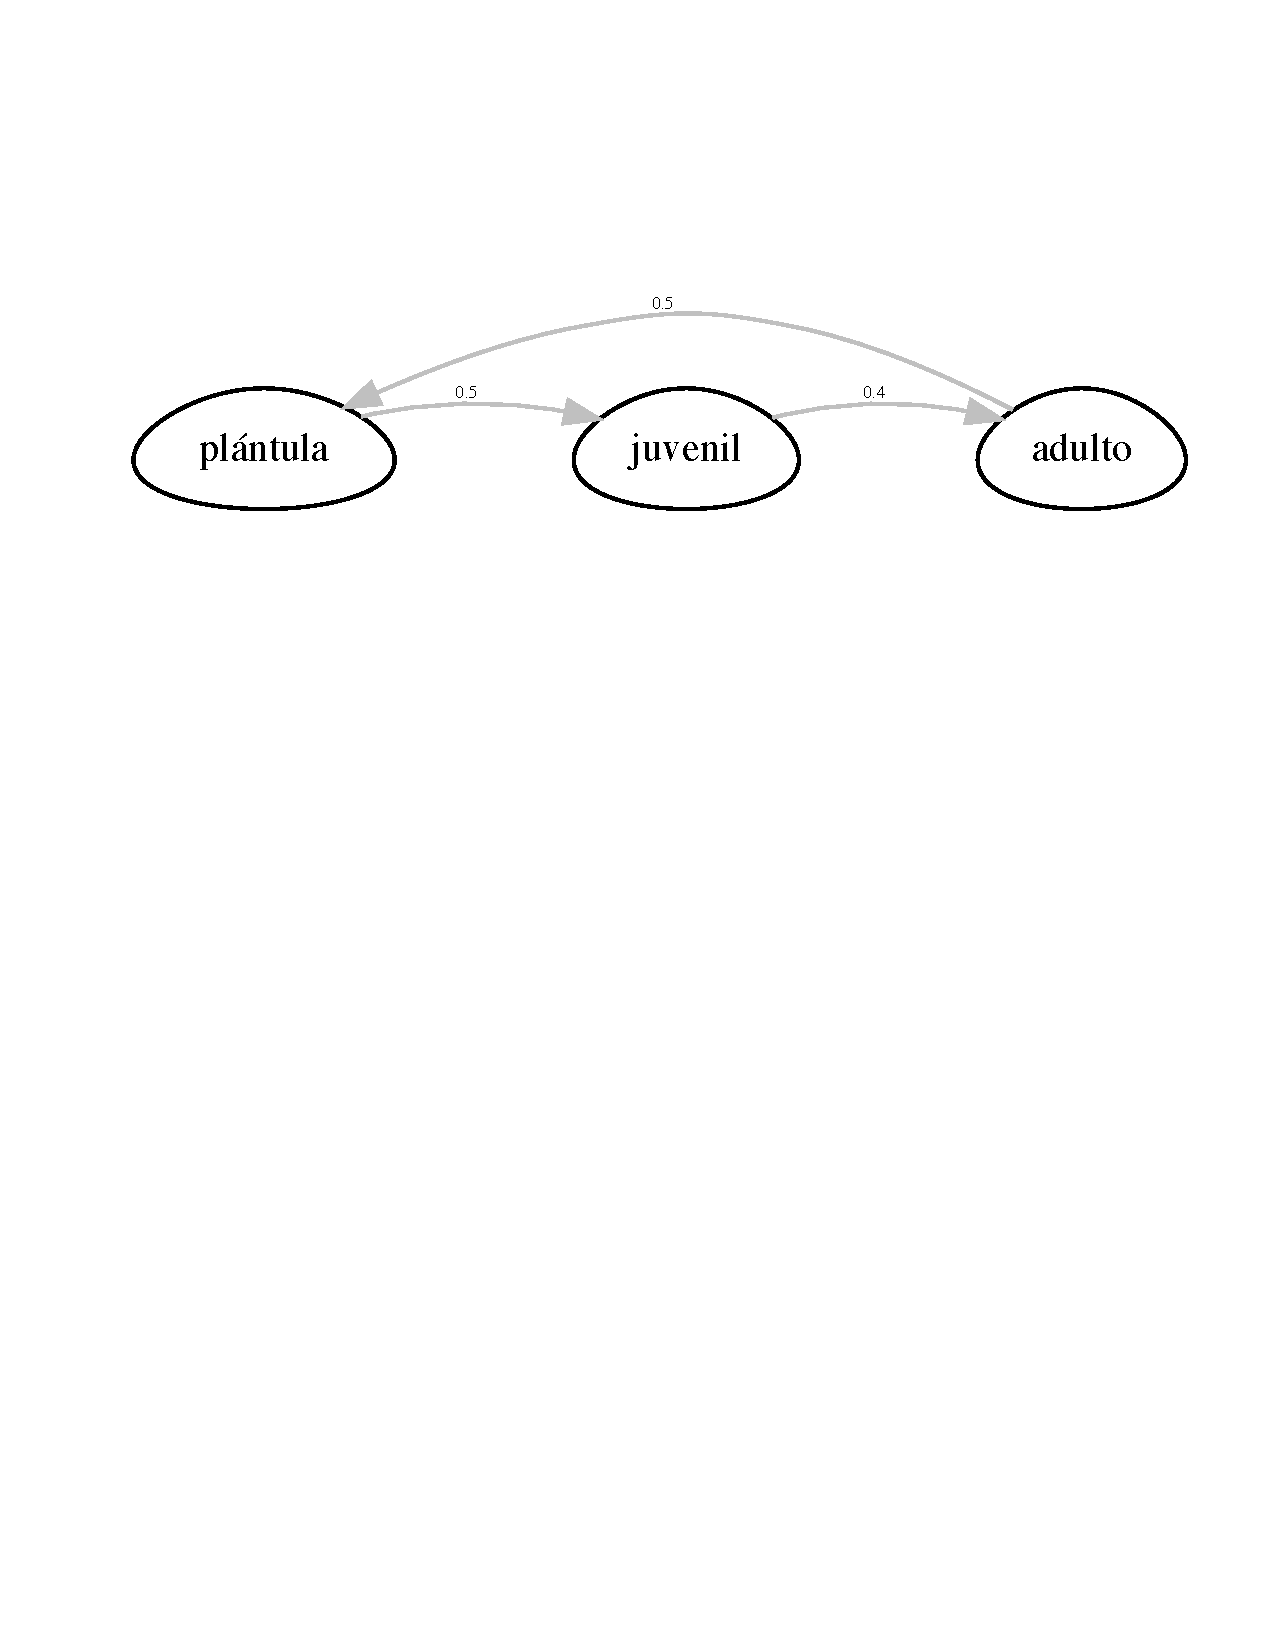
\includegraphics[keepaspectratio]{106-calcular_fecundidad_files/figure-pdf/unnamed-chunk-4-1.pdf}}

\begin{tcolorbox}[enhanced jigsaw, arc=.35mm, bottomrule=.15mm, bottomtitle=1mm, breakable, colback=white, colbacktitle=quarto-callout-tip-color!10!white, colframe=quarto-callout-tip-color-frame, coltitle=black, left=2mm, leftrule=.75mm, opacityback=0, opacitybacktitle=0.6, rightrule=.15mm, title=\textcolor{quarto-callout-tip-color}{\faLightbulb}\hspace{0.5em}{Recomendación}, titlerule=0mm, toprule=.15mm, toptitle=1mm]

\textbf{Tres maneras de estimar la fecundidad, ordenadas de la más
exigente a la más práctica.}

\begin{enumerate}
\def\labelenumi{\arabic{enumi}.}
\tightlist
\item
  \textbf{Vía completa:} semillas producidas × tasa de germinación ×
  tasa de supervivencia hasta plántula, dividido entre el número de
  adultos. Requiere mucha información empírica.
\item
  \textbf{Vía intermedia:} producción de frutos × estimación de la
  viabilidad y germinación de semillas. Útil cuando se dispone de datos
  parciales.
\item
  \textbf{Vía directa:} número de plántulas observadas en \(t_{+1}\)
  dividido entre número de adultos en \(t_0\). Es la más práctica cuando
  no hay datos de semillas/germinación, y la más usada en estudios de
  campo.
\end{enumerate}

La vía directa absorbe automáticamente las pérdidas a lo largo de la
cadena reproductiva, pero asume que las nuevas plántulas provienen de
los adultos del periodo anterior y no de inmigración o banco de
semillas.

\end{tcolorbox}

\begin{center}\rule{0.5\linewidth}{0.5pt}\end{center}

\section{Sesgos en las condiciones y cálculos de
fecundidad}\label{sesgos-en-las-condiciones-y-cuxe1lculos-de-fecundidad}

Para estimar la fecundidad en modelos poblacionales, es necesario asumir
ciertos supuestos fundamentales.

\begin{tcolorbox}[enhanced jigsaw, arc=.35mm, bottomrule=.15mm, bottomtitle=1mm, breakable, colback=white, colbacktitle=quarto-callout-warning-color!10!white, colframe=quarto-callout-warning-color-frame, coltitle=black, left=2mm, leftrule=.75mm, opacityback=0, opacitybacktitle=0.6, rightrule=.15mm, title=\textcolor{quarto-callout-warning-color}{\faExclamationTriangle}\hspace{0.5em}{Advertencia}, titlerule=0mm, toprule=.15mm, toptitle=1mm]

\textbf{Cuatro supuestos que se asumen al estimar fecundidad por
reclutamiento directo.}

\begin{itemize}
\tightlist
\item
  Las plántulas registradas en \(t_2\) provienen de los adultos en
  \(t_1\).
\item
  No hay inmigración desde otros sitios (o se modela explícitamente; ver
  (Pascarella \& Horvitz, 1998)).
\item
  No hay banco de semillas que aporte plántulas de cohortes anteriores.
\item
  El periodo de muestreo coincide con la ventana en que las plántulas
  son visibles.
\end{itemize}

Si alguno de estos supuestos se rompe, la fecundidad estimada será
sesgada. Conviene evaluar la plausibilidad de cada uno para la especie y
el sitio antes de aceptar el valor obtenido.

\end{tcolorbox}

Es importante reconocer que no existe un método perfecto para calcular
la fecundidad. El procedimiento descrito aquí es útil cuando no se
dispone de información sobre la cantidad de semillas producidas ni sobre
su supervivencia y germinación. Sin embargo, siempre existe la
posibilidad de que algunas semillas germinen en otros periodos o
provengan de sitios externos, lo que introduce sesgos. Mientras estos
sesgos sean mínimos, las estimaciones pueden considerarse aceptables
para expresar la fecundidad en términos de plántulas.

El escenario ideal sería seguir todo el proceso reproductivo:
cuantificar el esfuerzo reproductivo de cada individuo, registrar la
producción de semillas y monitorear su germinación en campo. No
obstante, este seguimiento completo es prácticamente imposible, por lo
que se deben asumir ciertos procesos biológicos, entre ellos:

\begin{itemize}
\tightlist
\item
  La cantidad de semillas por fruto es constante.
\item
  La calidad de las semillas (probabilidad de germinar) es homogénea
  entre frutos, aunque puede variar entre individuos debido a factores
  como autofecundación, exogamia o polinización múltiple. Las
  condiciones ecológicas necesarias para la germinación son similares.
\item
  El tiempo de germinación es comparable entre semillas (sin banco de
  semillas, salvo que esté implícitamente considerado en el modelo).
\item
  Diferentes tamaños o estadios de adultos pueden producir cantidades
  distintas de semillas o semillas de calidad variable.
\end{itemize}

\begin{center}\rule{0.5\linewidth}{0.5pt}\end{center}

\bookmarksetup{startatroot}

\chapter{Matrices de transición, fecundidad y reproducción
clonal}\label{MatricesTFC}

Las matrices U, F y C descomponen la dinámica poblacional en sus
componentes demográficos fundamentales: supervivencia y crecimiento,
fecundidad y transiciones complementarias. Este capítulo introduce estas
matrices como herramientas conceptuales y analíticas para representar
explícitamente los procesos que estructuran la dinámica poblacional.

Raymond L. Tremblay

\section{Descomposición matricial de la dinámica
poblacional}\label{descomposiciuxf3n-matricial-de-la-dinuxe1mica-poblacional}

En los modelos de proyección poblacional estructurados, la matriz de
proyección puede descomponerse en componentes que representan procesos
demográficos distintos. Las matrices \textbf{U}, \textbf{F} y \textbf{C}
permiten separar la dinámica poblacional en supervivencia y crecimiento
(U), fecundidad (F) y otras transiciones complementarias (C),
facilitando la interpretación biológica y analítica del modelo.

En este capítulo se presenta la lógica conceptual de esta
descomposición, mostrando cómo cada matriz captura un conjunto
específico de procesos del ciclo de vida. La matriz \textbf{U} describe
las transiciones no reproductivas entre estadios, incluyendo estasis y
crecimiento. La matriz \textbf{F} representa la contribución
reproductiva a los estadios iniciales, integrando producción
reproductiva y supervivencia temprana. En casos particulares, la matriz
\textbf{C} permite incorporar transiciones adicionales que no encajan
directamente en U o F, ampliando la flexibilidad del modelo.

La descomposición en U, F y C constituye un paso intermedio clave entre
la definición de transiciones individuales y el análisis de propiedades
poblacionales. Este enfoque permite evaluar separadamente el papel de
cada proceso demográfico en el crecimiento poblacional y sirve como base
para análisis posteriores de elasticidad, sensibilidad, LTRE y
simulaciones. A diferencia de capítulos previos, este capítulo se enfoca
en la representación estructural explícita de los procesos demográficos
dentro de la matriz, proporcionando un puente entre la biología del
ciclo de vida y las herramientas analíticas desarrolladas más adelante.

\subsubsection{Librerías de R requeridas para el siguiente
módulo}\label{libreruxedas-de-r-requeridas-para-el-siguiente-muxf3dulo-5}

\begin{Shaded}
\begin{Highlighting}[]
\FunctionTok{library}\NormalTok{(DiagrammeR)}
\FunctionTok{library}\NormalTok{(Rage)}
\FunctionTok{library}\NormalTok{(Rcompadre)}
\FunctionTok{library}\NormalTok{(dplyr)}
\FunctionTok{library}\NormalTok{(purrr)}
\end{Highlighting}
\end{Shaded}

\section{Construcción y cálculo de las matrices U, F y
C}\label{construcciuxf3n-y-cuxe1lculo-de-las-matrices-u-f-y-c}

A continuación se describe cómo definir y calcular las matrices U, F y C
a partir de transiciones demográficas y datos empíricos.

\section{Tres tipos de matrices}\label{tres-tipos-de-matrices}

Para facilitar los análisis e interpretaciones es necesario tener claro
el ciclo de vida de la especie y el origen de los parámetros de
transiciones, fecundidades y clonaje. Para lo cual, hay que recordar que
la matriz A (matA), para evaluar varios de los parámetros del
crecimiento poblacional, es el resultado de la suma de las submatrices
de transición, de fecundidad y de clonación. Un ejemplo de por qué es
necesario crear submatrices es que, para calcular la supervivencia
promedia y sus intervalos de confianza, se necesita la matriz de
transiciones \textbf{matU} separado de la matriz de fecundidad, mientras
que para calcular la tasa de crecimiento poblacional, se necesita
\textbf{matA}. En adición si uno quiere un estimado de la endogamia es
importante reconocer la importancia de la clonación en la dinámica
poblacional, se necesita incluir \textbf{matC}. Por consecuencia, es
importante tener claro el ciclo de vida y la forma de reproducción de la
especie que se está estudiando. La definición de las matrices U, F y C
se basa directamente en los procesos de transición descritos en el
capítulo sobre transiciones demográficas. La combinación de las matrices
U, F y C permite derivar la tasa de crecimiento poblacional discutida en
el capítulo sobre crecimiento poblacional.

Definiciones de las matrices

\begin{itemize}
\tightlist
\item
  MatU = Matriz de Transiciones
\item
  MatF = Matriz de Fecundidad
\item
  MatC = Matriz de Clonación
\item
  MatA = MatU + MatF + MatC
\end{itemize}

\begin{tcolorbox}[enhanced jigsaw, arc=.35mm, bottomrule=.15mm, bottomtitle=1mm, breakable, colback=white, colbacktitle=quarto-callout-note-color!10!white, colframe=quarto-callout-note-color-frame, coltitle=black, left=2mm, leftrule=.75mm, opacityback=0, opacitybacktitle=0.6, rightrule=.15mm, title=\textcolor{quarto-callout-note-color}{\faInfo}\hspace{0.5em}{Nota}, titlerule=0mm, toprule=.15mm, toptitle=1mm]

\textbf{Cada submatriz sirve análisis diferentes.}

\begin{itemize}
\tightlist
\item
  \texttt{matU} se usa para calcular \textbf{supervivencia, esperanza de
  vida y trayectorias por estadios} (no incluye la creación de nuevos
  individuos).
\item
  \texttt{matF} y \texttt{matC} se usan para evaluar
  \textbf{contribución reproductiva} (sexual o clonal) por separado.
\item
  \texttt{matA\ =\ matU\ +\ matF\ +\ matC} se usa para calcular
  \textbf{λ} y proyecciones poblacionales completas.
\end{itemize}

Mantenerlas separadas es la convención de bases de datos como COMPADRE y
permite recombinarlas según el análisis.

\end{tcolorbox}

\begin{figure}[H]

{\centering 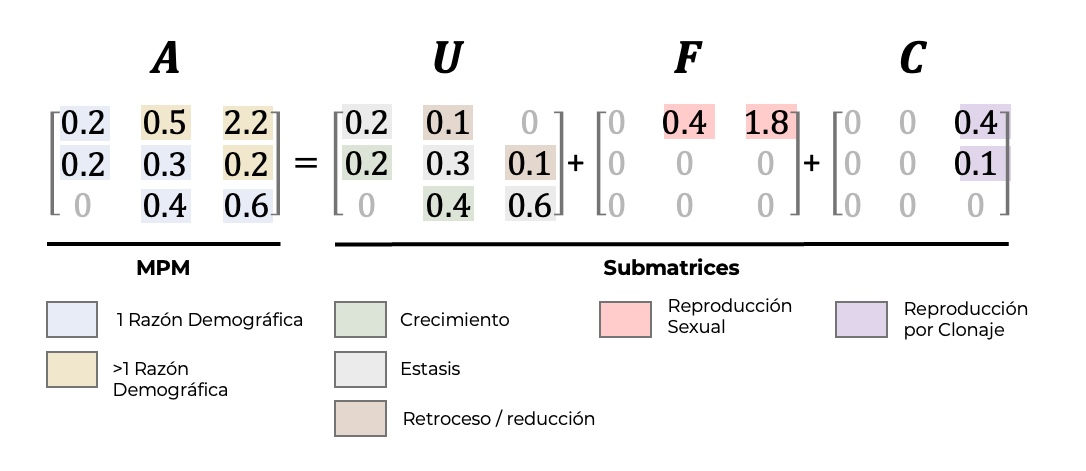
\includegraphics[width=0.9\linewidth,height=\textheight,keepaspectratio]{images/Matrices_A_U_F_C.jpg}

}

\caption{Relación entre matrices; Diseño: Samuel Gascoigne}

\end{figure}%

\begin{center}\rule{0.5\linewidth}{0.5pt}\end{center}

\section{MatU: Matriz de
transiciones}\label{matu-matriz-de-transiciones}

La matriz de transiciones \textbf{matU} contiene únicamente entradas que
representan cambios entre estados vitales: \textbf{crecimiento},
\textbf{permanencia (estasis)} y \textbf{retrogresión (decrecimiento)}.
Por lo tanto, toda la información relacionada con \textbf{reproducción}
y \textbf{clonación} está excluida de esta matriz.

Como ejemplo, consideremos un modelo con tres etapas de vida:
\textbf{plántulas}, \textbf{juveniles} y \textbf{adultos}, donde se
observan todas las transiciones posibles. En este modelo, los juveniles
\textbf{no pueden regresar a ser plántulas}, ya que fisiológicamente las
plántulas presentan características distintas a individuos que ya han
desarrollado raíces y hojas.\\

Recuerde que los individuos incluidos en un mismo estadio deben tener
\textbf{probabilidades similares de crecimiento, supervivencia y
fecundidad}.

En cambio, los adultos \textbf{sí pueden regresar a la etapa juvenil}
(al menos como individuos no reproductivos), posiblemente como
consecuencia de \textbf{daño por herbivoría}, que reduce su tamaño.

\begin{Shaded}
\begin{Highlighting}[]
\NormalTok{matU }\OtherTok{\textless{}{-}} \FunctionTok{rbind}\NormalTok{(}
  \FunctionTok{c}\NormalTok{(}\FloatTok{0.1}\NormalTok{, }\FloatTok{0.0}\NormalTok{, }\FloatTok{0.0}\NormalTok{),}
  \FunctionTok{c}\NormalTok{(}\FloatTok{0.5}\NormalTok{, }\FloatTok{0.3}\NormalTok{, }\FloatTok{0.05}\NormalTok{),}
  \FunctionTok{c}\NormalTok{(}\FloatTok{0.001}\NormalTok{, }\FloatTok{0.4}\NormalTok{, }\FloatTok{0.8}\NormalTok{)}
\NormalTok{)}
\NormalTok{stages }\OtherTok{\textless{}{-}} \FunctionTok{c}\NormalTok{(}\StringTok{"Plántulas"}\NormalTok{, }\StringTok{"Juvenil"}\NormalTok{, }\StringTok{"Adulto"}\NormalTok{)}
\FunctionTok{plot\_life\_cycle}\NormalTok{(matU, }\AttributeTok{stages =}\NormalTok{ stages)}
\end{Highlighting}
\end{Shaded}

\pandocbounded{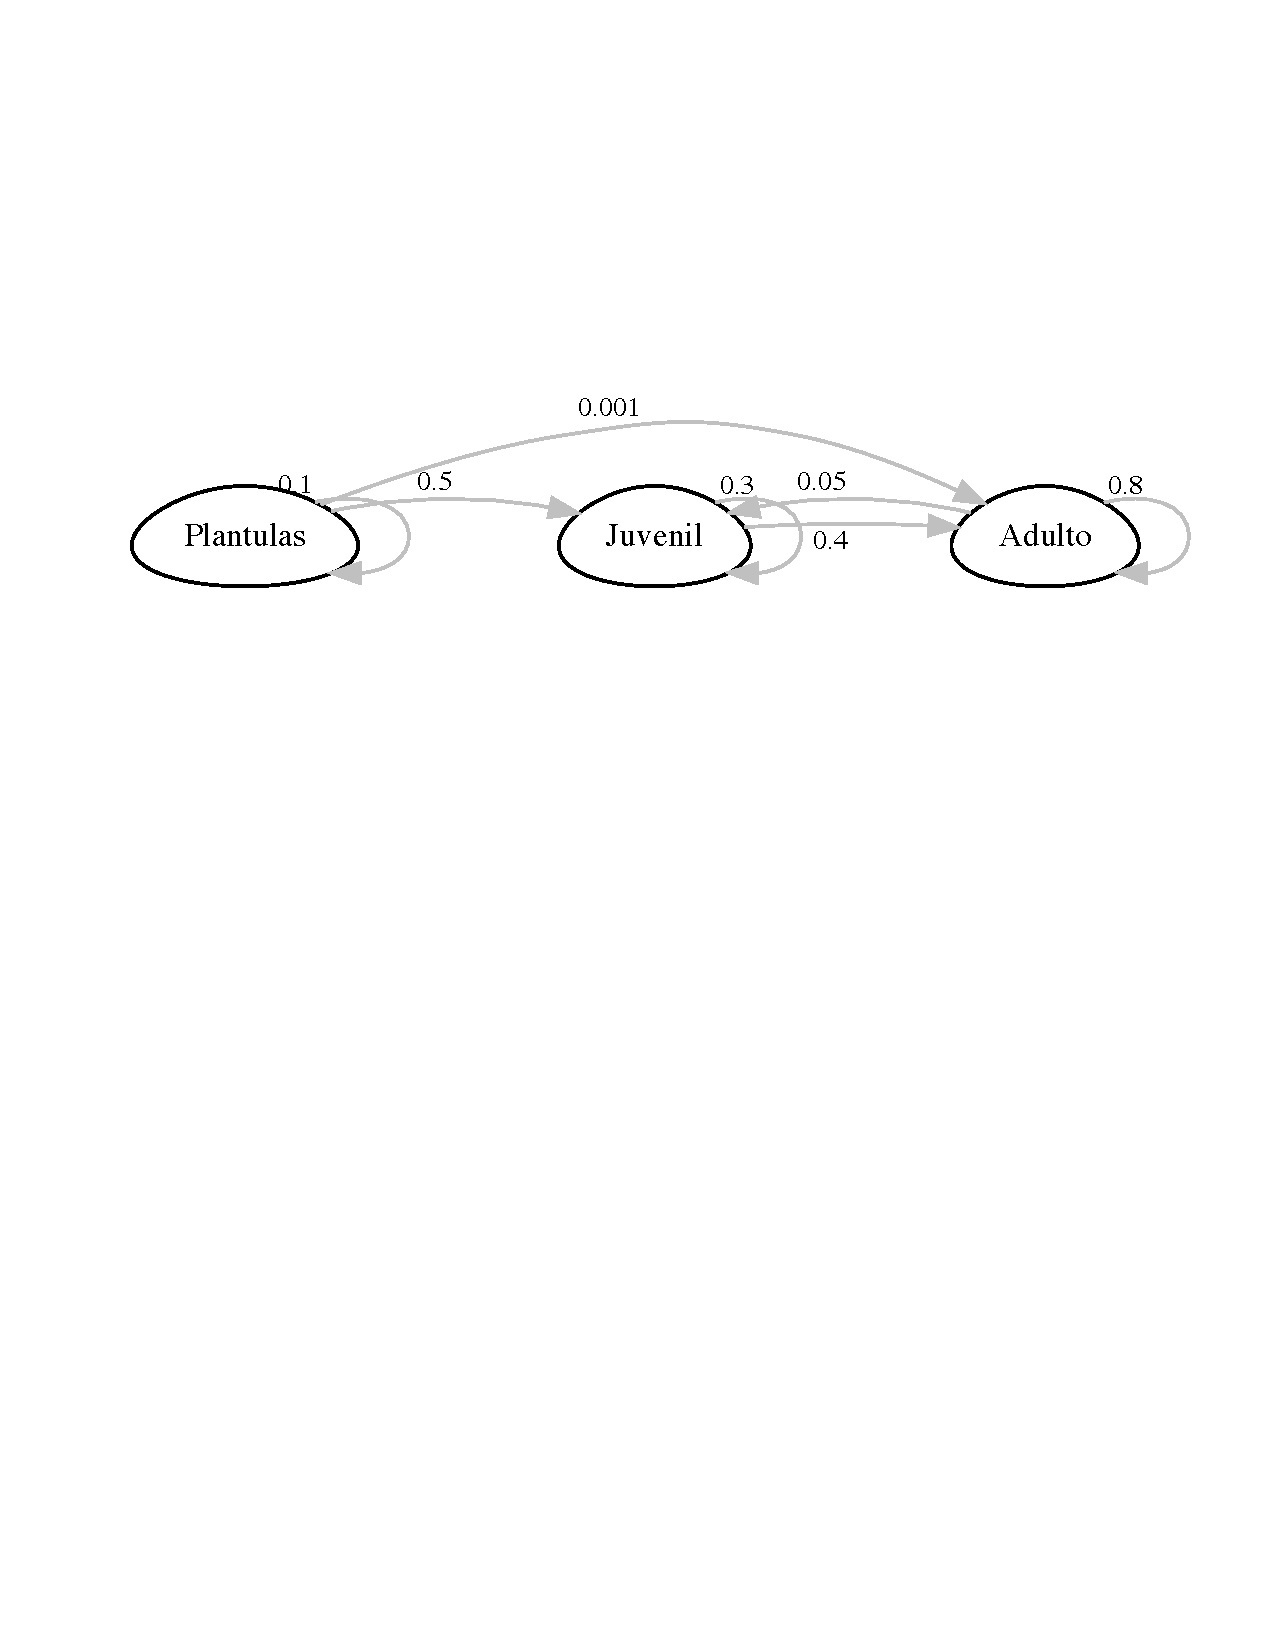
\includegraphics[keepaspectratio]{107-matU_matF_matC_files/figure-pdf/matA1-1.pdf}}

\begin{center}\rule{0.5\linewidth}{0.5pt}\end{center}

\section{MatF: Matriz de fecundidad}\label{matf-matriz-de-fecundidad}

La matriz F se construye a partir de los parámetros de fecundidad
calculados en el capítulo sobre cálculo de fecundidad. Al analizar la
figura siguiente, se observa que algunos individuos en la segunda etapa
pueden producir plántulas. Por ello, sería más apropiado cambiar el
nombre de esta etapa de ``juvenil'' a ``adultos pequeños'', ya que el
término juvenil podría interpretarse como individuos no reproductivos.

En el ciclo de vida se aprecia que las plántulas provienen tanto de
adultos pequeños como de adultos grandes. Esta separación en categorías
de adultos es recomendable cuando las probabilidades de fecundidad
difieren significativamente entre clases de tamaño.

Por ejemplo, en el estudio de la demografía de \emph{Guarianthe
aurantiaca} (Mondragón, 2009), se definieron dos categorías
reproductivas:

\begin{itemize}
\tightlist
\item
  adultos pequeños (r1): pseudobulbos entre 7 y 15 cm
\item
  adultos grandes (r2): pseudobulbos \textgreater{} 15 cm
\end{itemize}

Los resultados mostraron una gran diferencia en la producción de
plántulas:

\begin{itemize}
\tightlist
\item
  r1: 0.007
\item
  r2: 0.121.
\end{itemize}

\begin{Shaded}
\begin{Highlighting}[]
\NormalTok{matF }\OtherTok{\textless{}{-}} \FunctionTok{rbind}\NormalTok{(}
  \FunctionTok{c}\NormalTok{(}\FloatTok{0.0}\NormalTok{, }\FloatTok{0.007}\NormalTok{, }\FloatTok{0.121}\NormalTok{),}
  \FunctionTok{c}\NormalTok{(}\FloatTok{0.0}\NormalTok{, }\FloatTok{0.0}\NormalTok{, }\FloatTok{0.0}\NormalTok{),}
  \FunctionTok{c}\NormalTok{(}\FloatTok{0.0}\NormalTok{, }\FloatTok{0.0}\NormalTok{, }\FloatTok{0.0}\NormalTok{)}
\NormalTok{)}
\NormalTok{stages }\OtherTok{\textless{}{-}} \FunctionTok{c}\NormalTok{(}\StringTok{"Plántulas"}\NormalTok{, }\StringTok{"Adultos Pequeños"}\NormalTok{, }\StringTok{"Adultos Grandes"}\NormalTok{)}
\FunctionTok{plot\_life\_cycle}\NormalTok{(matF, }\AttributeTok{stages =}\NormalTok{ stages)}
\end{Highlighting}
\end{Shaded}

\pandocbounded{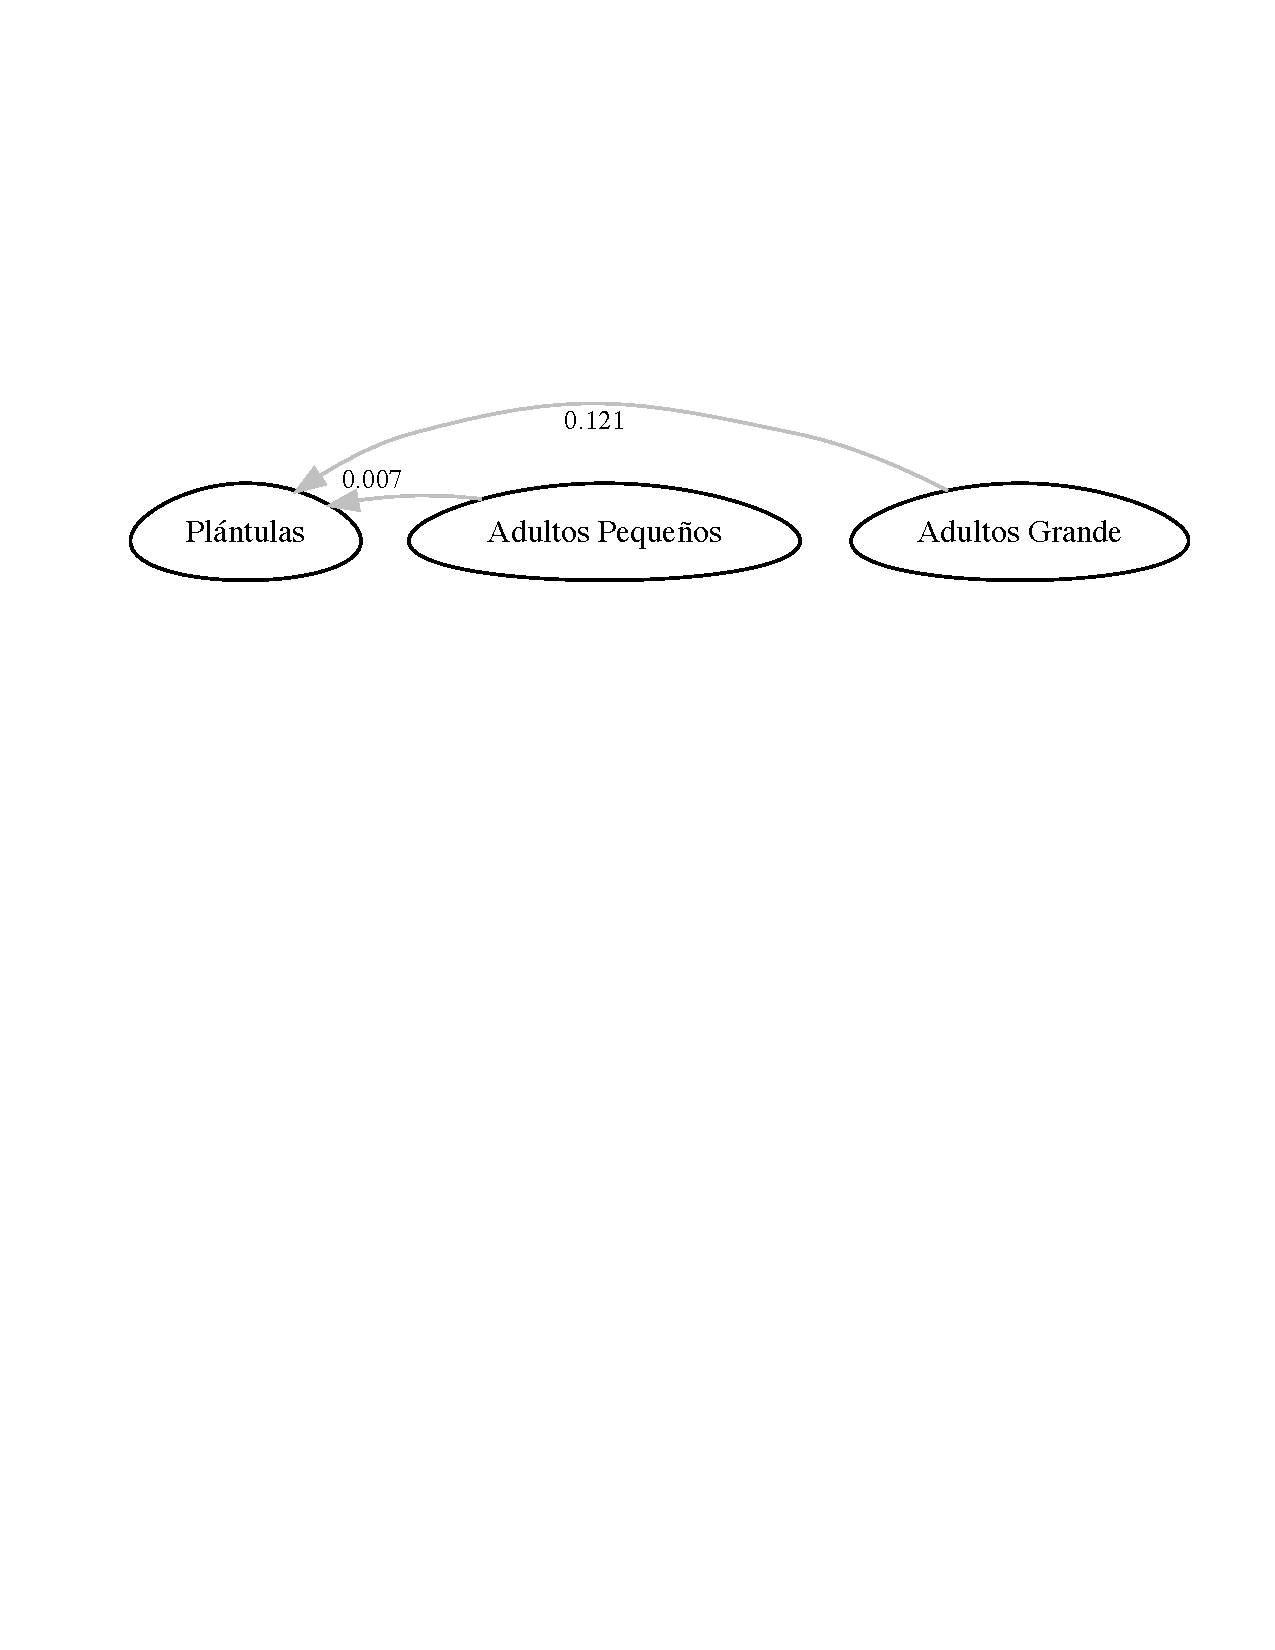
\includegraphics[keepaspectratio]{107-matU_matF_matC_files/figure-pdf/matA2-1.pdf}}

\begin{center}\rule{0.5\linewidth}{0.5pt}\end{center}

\section{MatC = Matriz de clonación}\label{matc-matriz-de-clonaciuxf3n}

Esta matriz representa la contribución de la reproducción asexual en la
dinámica poblacional. Es fundamental comprender que la propagación
vegetativa origina un ramet, un individuo ecológicamente independiente,
aunque genéticamente idéntico al progenitor (genet) (Cook, 1983).

Por ejemplo:

\begin{itemize}
\tightlist
\item
  En \emph{Epidendrum}, la producción de nuevos tallos no se considera
  reproducción, ya que permanecen unidos y conectados, funcionando más
  como crecimiento que como reproducción. El destino demográfico de cada
  tallo depende del resto, similar a las ramas de un árbol.
\item
  En \emph{Artorima erubescens}, las cadenas de pseudobulbos pueden
  fragmentarse, y cada sección tiene un destino demográfico
  independiente. En este caso, sí hablamos de reproducción vegetativa
  (García-Soriano, 2003).
\item
  En especies que producen keikis, cada keiki se convierte en un nuevo
  individuo ecológico al separarse de la planta madre, con crecimiento,
  supervivencia y fecundidad independientes.
\end{itemize}

\textbf{¿Por qué no incluir ramets en la matriz de fecundidad (matF)?}

Los individuos generados por propagación vegetativa difieren
radicalmente de las plántulas:

\begin{itemize}
\tightlist
\item
  Las plántulas provienen de semillas, mientras que los ramets surgen de
  meristemos.
\item
  Los ramets suelen tener tasas mucho mayores de crecimiento y
  supervivencia, ya que reciben recursos de la planta madre mientras
  permanecen conectados.
\end{itemize}

Por ello, su incorporación en la matriz ocurre generalmente en estadios
superiores. El aporte se hace a la categoría de juveniles. Esto puede
provocar que en la matriz \textbf{matA} las entradas superen el rango
típico (0--1), ya que se suman transiciones y fecundidad vía ramets.

\begin{tcolorbox}[enhanced jigsaw, arc=.35mm, bottomrule=.15mm, bottomtitle=1mm, breakable, colback=white, colbacktitle=quarto-callout-note-color!10!white, colframe=quarto-callout-note-color-frame, coltitle=black, left=2mm, leftrule=.75mm, opacityback=0, opacitybacktitle=0.6, rightrule=.15mm, title=\textcolor{quarto-callout-note-color}{\faInfo}\hspace{0.5em}{Nota}, titlerule=0mm, toprule=.15mm, toptitle=1mm]

\textbf{Las entradas de \texttt{matA} pueden superar 1 cuando hay
clonaje.} En matrices puramente de transiciones (\texttt{matU}), cada
columna suma a lo sumo 1 (incluyendo la mortalidad implícita). Pero al
sumar \texttt{matU\ +\ matF\ +\ matC}, las entradas individuales pueden
superar 1 porque un mismo individuo puede contribuir simultáneamente a
varios destinos: sobrevivir y crecer (\texttt{matU}), producir plántulas
sexuales (\texttt{matF}), y aportar \emph{ramets} (\texttt{matC}). Una
entrada \textgreater{} 1 en \texttt{matA} no es un error --- refleja que
la columna ya no es una distribución de probabilidades de destino, sino
una contabilidad de transiciones más reclutas.

\end{tcolorbox}

\begin{center}\rule{0.5\linewidth}{0.5pt}\end{center}

\subsection{Clonación: Diferencia entre ramet y
genet}\label{clonaciuxf3n-diferencia-entre-ramet-y-genet}

\begin{tcolorbox}[enhanced jigsaw, arc=.35mm, bottomrule=.15mm, bottomtitle=1mm, breakable, colback=white, colbacktitle=quarto-callout-important-color!10!white, colframe=quarto-callout-important-color-frame, coltitle=black, left=2mm, leftrule=.75mm, opacityback=0, opacitybacktitle=0.6, rightrule=.15mm, title=\textcolor{quarto-callout-important-color}{\faExclamation}\hspace{0.5em}{Importante}, titlerule=0mm, toprule=.15mm, toptitle=1mm]

\textbf{Genet versus \emph{ramet}.}

\begin{itemize}
\tightlist
\item
  \textbf{Genet:} la unidad genética --- todos los individuos que
  descienden de una misma semilla y comparten el genoma original.
\item
  \textbf{\emph{Ramet}:} la unidad ecológica --- cada módulo o tallo que
  puede sobrevivir, crecer y reproducirse de forma independiente.
\end{itemize}

Una orquídea con varios pseudobulbos puede ser un genet con muchos
\emph{ramets}. Los modelos demográficos típicamente cuentan
\emph{ramets} (porque cada uno es un individuo ecológicamente
independiente), no genets --- pero esta convención afecta directamente
cómo se interpretan tasas de ``supervivencia'' y ``fecundidad''.

\end{tcolorbox}

Al estudiar especies con reproducción clonal, es esencial diferenciar
entre ramet y genet:

\begin{itemize}
\tightlist
\item
  Genet: conjunto de todos los ramets que comparten la misma identidad
  genética.
\item
  Ramet: cada unidad individual dentro del genet, ecológicamente
  independiente pero genéticamente idéntica.
\end{itemize}

En orquídeas, cada seudobulbo puede considerarse un ramet, mientras que
la suma de todos los seudobulbos conforma el genet. Existen enfoques
para incorporar esta distinción en las matrices demográficas y, por
ende, integrar el concepto de clonación en los estimados de adecuación
(McGraw \& Caswell, 1996).

\subsection{Ejemplo de matriz de
clonación}\label{ejemplo-de-matriz-de-clonaciuxf3n}

A continuación, se muestra un ejemplo de matriz de clonación. En la base
de datos COMPADRE, el único caso registrado corresponde a
\emph{Cypripedium calceolus} (Garcı́a González, Goñi \& Guzmán, 2010).
Este ejemplo también permite ilustrar cómo extraer matrices con
características específicas desde la base de datos COMPADRE.

\begin{center}\rule{0.5\linewidth}{0.5pt}\end{center}

\subsection{Descargar la base de datos de
COMPADRE}\label{descargar-la-base-de-datos-de-compadre}

\begin{Shaded}
\begin{Highlighting}[]
\NormalTok{compadre }\OtherTok{\textless{}{-}} \FunctionTok{readRDS}\NormalTok{(}\StringTok{"data/COMPADRE\_2026.rds"}\NormalTok{)}
\end{Highlighting}
\end{Shaded}

\begin{center}\rule{0.5\linewidth}{0.5pt}\end{center}

\section{Extraer MPP con matriz de
clonaje}\label{extraer-mpp-con-matriz-de-clonaje}

En el siguiente script se calcula la suma de todos los valores de la
matriz de clonación (\textbf{matC}). Cualquier especie que presente un
valor mayor a 0 en esta matriz se considera que posee clonación en al
menos una etapa de su ciclo de vida.

Del análisis se observa que 8,304 especies no tienen información
registrada en \textbf{matC}. Por otro lado, una población cuya suma en
matC sea superior a cero (por ejemplo, ≥ 0.001) se clasifica como una
especie con clonación.

\begin{Shaded}
\begin{Highlighting}[]
\NormalTok{compadre }\OtherTok{\textless{}{-}} \FunctionTok{readRDS}\NormalTok{(}\StringTok{"data/COMPADRE\_2026.rds"}\NormalTok{)}

\CommentTok{\#Encontrar MPP con matC clonaje no cero}
\NormalTok{compadre}\SpecialCharTok{$}\NormalTok{clonality }\OtherTok{\textless{}{-}} \DecValTok{0}


\NormalTok{compadre}\SpecialCharTok{$}\NormalTok{clonality }\OtherTok{\textless{}{-}} \FunctionTok{sapply}\NormalTok{(compadre}\SpecialCharTok{$}\NormalTok{mat, }\ControlFlowTok{function}\NormalTok{(m) }\FunctionTok{sum}\NormalTok{(m}\SpecialCharTok{@}\NormalTok{matC))}

\CommentTok{\#table(compadre$clonality) \# Remover el "\#" para ver todos los resultados,}

\FunctionTok{as.data.frame}\NormalTok{(}\FunctionTok{head}\NormalTok{(}\FunctionTok{table}\NormalTok{(compadre}\SpecialCharTok{$}\NormalTok{clonality))) }\SpecialCharTok{|\textgreater{}} \FunctionTok{flextable}\NormalTok{() }\CommentTok{\#Se observa la suma de las matrices de clonaje, hay 8304 especies que no tiene información en matC, una población con un matC que su suma es 0.001, etc.}
\end{Highlighting}
\end{Shaded}

\begin{verbatim}
Error in `flextable()`:
! could not find function "flextable"
\end{verbatim}

\begin{Shaded}
\begin{Highlighting}[]
\FunctionTok{summary}\NormalTok{(compadre}\SpecialCharTok{$}\NormalTok{clonality[compadre}\SpecialCharTok{$}\NormalTok{clonality}\SpecialCharTok{\textgreater{}}\DecValTok{0}\NormalTok{],) }\CommentTok{\# Resumen estadístico de la clonación en la base de datos de las especies que tienen clonación}
\end{Highlighting}
\end{Shaded}

\begin{verbatim}
    Min.  1st Qu.   Median     Mean  3rd Qu.     Max.     NA's 
  0.0010   0.2625   0.8550   3.4643   2.2227 347.3600        7 
\end{verbatim}

\begin{Shaded}
\begin{Highlighting}[]
\CommentTok{\# crear un histograma de las especies que tienen clonación (excluir las especies que no tiene clonación)}

\CommentTok{\#hist(compadre$clonality[compadre$clonality \textgreater{} 0], breaks = 50, main = "Histogram of \#Clonality in COMPADRE", xlab = "Clonality (sum of matC)", ylab = "Frequency")}
\end{Highlighting}
\end{Shaded}

\begin{center}\rule{0.5\linewidth}{0.5pt}\end{center}

\subsection{Control de calidad de las
matrices}\label{control-de-calidad-de-las-matrices}

Es fundamental aplicar controles de calidad a la base de datos, por
ejemplo, para detectar entradas faltantes en la matriz principal
(\textbf{matA}).

En el capítulo COMPADRE y las orquídeas se utiliza esta base de datos y
se describen diversas estrategias para limpieza y selección de matrices
con características específicas, garantizando que los análisis se
realicen sobre datos completos y confiables.

\begin{Shaded}
\begin{Highlighting}[]
\NormalTok{compadre\_flagged }\OtherTok{\textless{}{-}} \FunctionTok{cdb\_flag}\NormalTok{(compadre, }\AttributeTok{checks =} \StringTok{"check\_NA\_A"}\NormalTok{) }\CommentTok{\# Evaluar que la matA no es nula (no suma a zero)}
\end{Highlighting}
\end{Shaded}

\begin{center}\rule{0.5\linewidth}{0.5pt}\end{center}

\section{Orquídeas con clonaje}\label{orquuxeddeas-con-clonaje}

Ahora filtrar para orquídeas solamente y para aquellos con \textbf{matC}
no nulo (clonality \textgreater0). Se observa que solamente dos
poblaciones tienen información de clonación.

\begin{Shaded}
\begin{Highlighting}[]
\NormalTok{orchid\_clonal }\OtherTok{\textless{}{-}}\NormalTok{ compadre\_flagged }\SpecialCharTok{\%\textgreater{}\%}
  \FunctionTok{filter}\NormalTok{(Family }\SpecialCharTok{==} \StringTok{"Orchidaceae"}\NormalTok{) }\SpecialCharTok{\%\textgreater{}\%} \CommentTok{\# filtrar para orquídeas}
  \FunctionTok{filter}\NormalTok{(clonality }\SpecialCharTok{\textgreater{}} \DecValTok{0}\NormalTok{) }\CommentTok{\# filtrar para aquellos con matC no nulo}

\CommentTok{\# Visualizar la base de datos de orquídea, se observa solamente dos matrices de clonaje}

\FunctionTok{unique}\NormalTok{(orchid\_clonal}\SpecialCharTok{$}\NormalTok{SpeciesAuthor) }\CommentTok{\# hay dos poblaciones solamente en toda la base de datos}
\end{Highlighting}
\end{Shaded}

\begin{verbatim}
[1] "Cypripedium_calceolus_2" "Cypripedium_calceolus_3"
\end{verbatim}

\begin{center}\rule{0.5\linewidth}{0.5pt}\end{center}

\subsection{\texorpdfstring{El estudio de \emph{Cypripedium
calceolus}}{El estudio de Cypripedium calceolus}}\label{el-estudio-de-cypripedium-calceolus}

Seleccionamos solamente un ejemplo, la Matriz de \emph{Cypripedium
calceolus} \#242624 (Garcı́a González, Goñi \& Guzmán, 2010), que es la
matriz promedio de la tercera población (SpeciesAuthor ==
Cypripedium\_calceolus\_3).

\begin{Shaded}
\begin{Highlighting}[]
\NormalTok{Cyp\_cal\_2 }\OtherTok{\textless{}{-}}\NormalTok{ orchid\_clonal }\SpecialCharTok{\%\textgreater{}\%}
  \FunctionTok{filter}\NormalTok{(MatrixID }\SpecialCharTok{==} \DecValTok{242624}\NormalTok{)}

\CommentTok{\#Cyp\_cal\_2}
\end{Highlighting}
\end{Shaded}

\begin{center}\rule{0.5\linewidth}{0.5pt}\end{center}

\subsubsection{\texorpdfstring{Buscar la población que tiene
\textbf{matC}
máxima.}{Buscar la población que tiene matC máxima.}}\label{buscar-la-poblaciuxf3n-que-tiene-matc-muxe1xima.}

En esta código, se evaluá todas las orquídeas donde tiene una matriz de
clonaje y se filtra para la que tiene la suma de matC máxima. En este
caso, es la misma población que se seleccionó en el script anterior.

\begin{Shaded}
\begin{Highlighting}[]
\CommentTok{\# Reemplace el bucle for de mat5 con esto:}
\NormalTok{compadre}\SpecialCharTok{$}\NormalTok{clonality }\OtherTok{\textless{}{-}} \FunctionTok{sapply}\NormalTok{(compadre}\SpecialCharTok{$}\NormalTok{mat, }\ControlFlowTok{function}\NormalTok{(m) }\FunctionTok{sum}\NormalTok{(m}\SpecialCharTok{@}\NormalTok{matC))}

\NormalTok{Orchid\_clonal\_max}\OtherTok{=}\NormalTok{orchid\_clonal }\SpecialCharTok{\%\textgreater{}\%}
  \FunctionTok{filter}\NormalTok{(clonality }\SpecialCharTok{==} \FunctionTok{max}\NormalTok{(clonality)) }\CommentTok{\# filtrar para la suma de matC máximo}

\NormalTok{Orchid\_clonal\_max}
\end{Highlighting}
\end{Shaded}

\begin{verbatim}
A COM(P)ADRE database ('CompadreDB') object with 1 SPECIES and 1 MATRICES.

# A tibble: 1 x 61
  mat        MatrixID SpeciesAuthor    SpeciesAccepted CommonName Kingdom Phylum
  <list>        <int> <chr>            <chr>           <chr>      <chr>   <chr> 
1 <CompdrMt>   242624 Cypripedium_cal~ Cypripedium ca~ Lady slip~ Plantae Magno~
# i 54 more variables: Class <chr>, Order <chr>, Family <chr>, Genus <chr>,
#   Species <chr>, Infraspecies <chr>, InfraspeciesType <chr>,
#   OrganismType <chr>, DicotMonoc <chr>, AngioGymno <chr>, Authors <chr>,
#   Journal <chr>, SourceType <chr>, OtherType <chr>, YearPublication <chr>,
#   DOI_ISBN <chr>, AdditionalSource <chr>, StudyDuration <chr>,
#   StudyStart <chr>, StudyEnd <chr>, ProjectionInterval <chr>,
#   MatrixCriteriaSize <chr>, MatrixCriteriaOntogeny <chr>, ...
\end{verbatim}

\begin{center}\rule{0.5\linewidth}{0.5pt}\end{center}

\subsubsection{\texorpdfstring{El estudio de \emph{Cypripedium
calceolus}}{El estudio de Cypripedium calceolus}}\label{el-estudio-de-cypripedium-calceolus-1}

Seleccionamos como ejemplo la matriz correspondiente a \emph{Cypripedium
calceolus} (ID \#242624) (Garcı́a González, Goñi \& Guzmán, 2010). Este
estudio tuvo como objetivo evaluar la hipótesis del modelo
central-marginal, que plantea que las poblaciones situadas en los
márgenes de su distribución son más susceptibles que aquellas ubicadas
en el centro. La especie fue modelada con base en 6 etapas, ``muy
pequeñas'', ``pequeñas'', ``intermedias'', ``grandes'', ``muy grandes''
y ``extra grandes'', más una etapa de ``latencia''. García et al.
(Garcı́a González, Goñi \& Guzmán, 2010) señalan que en \emph{Cypripedium
calceolus} es difícil diferenciar entre reclutamiento sexual y asexual,
y que la percepción de reclutamiento asexual probablemente sea mucho más
común que la sexual (Kull, 1995; Garcı́a González, Goñi \& Guzmán, 2010).

\begin{Shaded}
\begin{Highlighting}[]
\NormalTok{Cyp\_cal\_2 }\OtherTok{\textless{}{-}}\NormalTok{ orchid\_clonal }\SpecialCharTok{\%\textgreater{}\%}
  \FunctionTok{filter}\NormalTok{(MatrixID }\SpecialCharTok{==} \DecValTok{242624}\NormalTok{)}

\NormalTok{Cyp\_cal\_2}
\end{Highlighting}
\end{Shaded}

\begin{verbatim}
A COM(P)ADRE database ('CompadreDB') object with 1 SPECIES and 1 MATRICES.

# A tibble: 1 x 61
  mat        MatrixID SpeciesAuthor    SpeciesAccepted CommonName Kingdom Phylum
  <list>        <int> <chr>            <chr>           <chr>      <chr>   <chr> 
1 <CompdrMt>   242624 Cypripedium_cal~ Cypripedium ca~ Lady slip~ Plantae Magno~
# i 54 more variables: Class <chr>, Order <chr>, Family <chr>, Genus <chr>,
#   Species <chr>, Infraspecies <chr>, InfraspeciesType <chr>,
#   OrganismType <chr>, DicotMonoc <chr>, AngioGymno <chr>, Authors <chr>,
#   Journal <chr>, SourceType <chr>, OtherType <chr>, YearPublication <chr>,
#   DOI_ISBN <chr>, AdditionalSource <chr>, StudyDuration <chr>,
#   StudyStart <chr>, StudyEnd <chr>, ProjectionInterval <chr>,
#   MatrixCriteriaSize <chr>, MatrixCriteriaOntogeny <chr>, ...
\end{verbatim}

\begin{center}\rule{0.5\linewidth}{0.5pt}\end{center}

\subsubsection{\texorpdfstring{Las etapas del ciclo de vida de
\emph{Cypripedium calceolus}
son:}{Las etapas del ciclo de vida de Cypripedium calceolus son:}}\label{las-etapas-del-ciclo-de-vida-de-cypripedium-calceolus-son}

Aquí visualizamos las etapas del ciclo de vida de \emph{Cypripedium
calceolus} y la matriz de transición, fecundidad y clonación.

\begin{Shaded}
\begin{Highlighting}[]
\NormalTok{Cyp\_cal\_2}\SpecialCharTok{$}\NormalTok{mat[[}\DecValTok{1}\NormalTok{]] }\CommentTok{\#[[1]] ver las etapas del ciclo de vida de esta población con las tres matrices}
\end{Highlighting}
\end{Shaded}

\begin{verbatim}
  MatrixClassOrganized MatrixClassAuthor
1                 dorm           Dormant
2               active          Smallest
3               active             Small
4               active      Intermediate
5               active             Large
6               active       Extra large

matA:
     1    2    3    4    5    6
1 0.20 0.04 0.03 0.04 0.03 0.00
2 0.00 0.35 0.05 0.04 0.08 0.12
3 0.16 0.43 0.39 0.17 0.06 0.09
4 0.15 0.00 0.31 0.52 0.13 0.15
5 0.49 0.00 0.11 0.29 0.68 0.46
6 0.00 0.00 0.00 0.00 0.07 0.60

matU:
     1    2    3    4    5   6
1 0.20 0.04 0.03 0.04 0.03 0.0
2 0.00 0.35 0.00 0.00 0.00 0.0
3 0.16 0.43 0.39 0.00 0.00 0.0
4 0.15 0.00 0.31 0.52 0.13 0.0
5 0.49 0.00 0.11 0.29 0.68 0.4
6 0.00 0.00 0.00 0.00 0.07 0.6

matF:
  1 2    3    4    5    6
1 0 0 0.00 0.00 0.00 0.00
2 0 0 0.05 0.04 0.08 0.12
3 0 0 0.00 0.00 0.00 0.00
4 0 0 0.00 0.00 0.00 0.00
5 0 0 0.00 0.00 0.00 0.00
6 0 0 0.00 0.00 0.00 0.00

matC:
  1 2 3    4    5    6
1 0 0 0 0.00 0.00 0.00
2 0 0 0 0.00 0.00 0.00
3 0 0 0 0.17 0.06 0.09
4 0 0 0 0.00 0.00 0.15
5 0 0 0 0.00 0.00 0.06
6 0 0 0 0.00 0.00 0.00
\end{verbatim}

\begin{center}\rule{0.5\linewidth}{0.5pt}\end{center}

\subsubsection{Visualizar la transición de las diferentes etapas por
clonación
solamente}\label{visualizar-la-transiciuxf3n-de-las-diferentes-etapas-por-clonaciuxf3n-solamente}

Podemos visualizar las transiciones de las diferentes etapas por
clonación. Usa la función \texttt{plot\_life\_cycle} de la librería
\textbf{Rage} para visualizar el ciclo de vida. En este caso, las etapas
son ``Dormant'', ``Smallest'', ``Small'', ``Inter'', ``Large'',
``ExtraLarge'' y la matriz de clonación es la \textbf{matC}. Si se
reemplaza la matriz de clonación por la matriz \textbf{matA} se puede
ver el ciclo de vida con todas las transiciones, fecundidad y clonación.

\begin{Shaded}
\begin{Highlighting}[]
\CommentTok{\#remotes::install\_github("jonesor/Rage") \# Instalar de Github para la más reciente versión}
\FunctionTok{library}\NormalTok{(Rage)}

\NormalTok{matC }\OtherTok{=} \FunctionTok{matC}\NormalTok{(Cyp\_cal\_2) }\CommentTok{\# extraemos la matriz de clonación de este especie/población}

\FunctionTok{plot\_life\_cycle}\NormalTok{(}
\NormalTok{  matC[[}\DecValTok{1}\NormalTok{]], }\CommentTok{\# Note aqui se seleciona solamente la matriz de clonaje}
  \AttributeTok{stages =} \FunctionTok{c}\NormalTok{(}\StringTok{"Dormant"}\NormalTok{, }\StringTok{"Smallest"}\NormalTok{, }\StringTok{"Small"}\NormalTok{, }\StringTok{"Inter"}\NormalTok{, }\StringTok{"Large"}\NormalTok{, }\StringTok{"ExtraLarge"}\NormalTok{),}
  \AttributeTok{node\_order =} \FunctionTok{c}\NormalTok{(}\DecValTok{2}\NormalTok{, }\DecValTok{1}\NormalTok{, }\DecValTok{3}\NormalTok{, }\DecValTok{4}\NormalTok{, }\DecValTok{5}\NormalTok{, }\DecValTok{6}\NormalTok{)}
\NormalTok{)}
\end{Highlighting}
\end{Shaded}

\pandocbounded{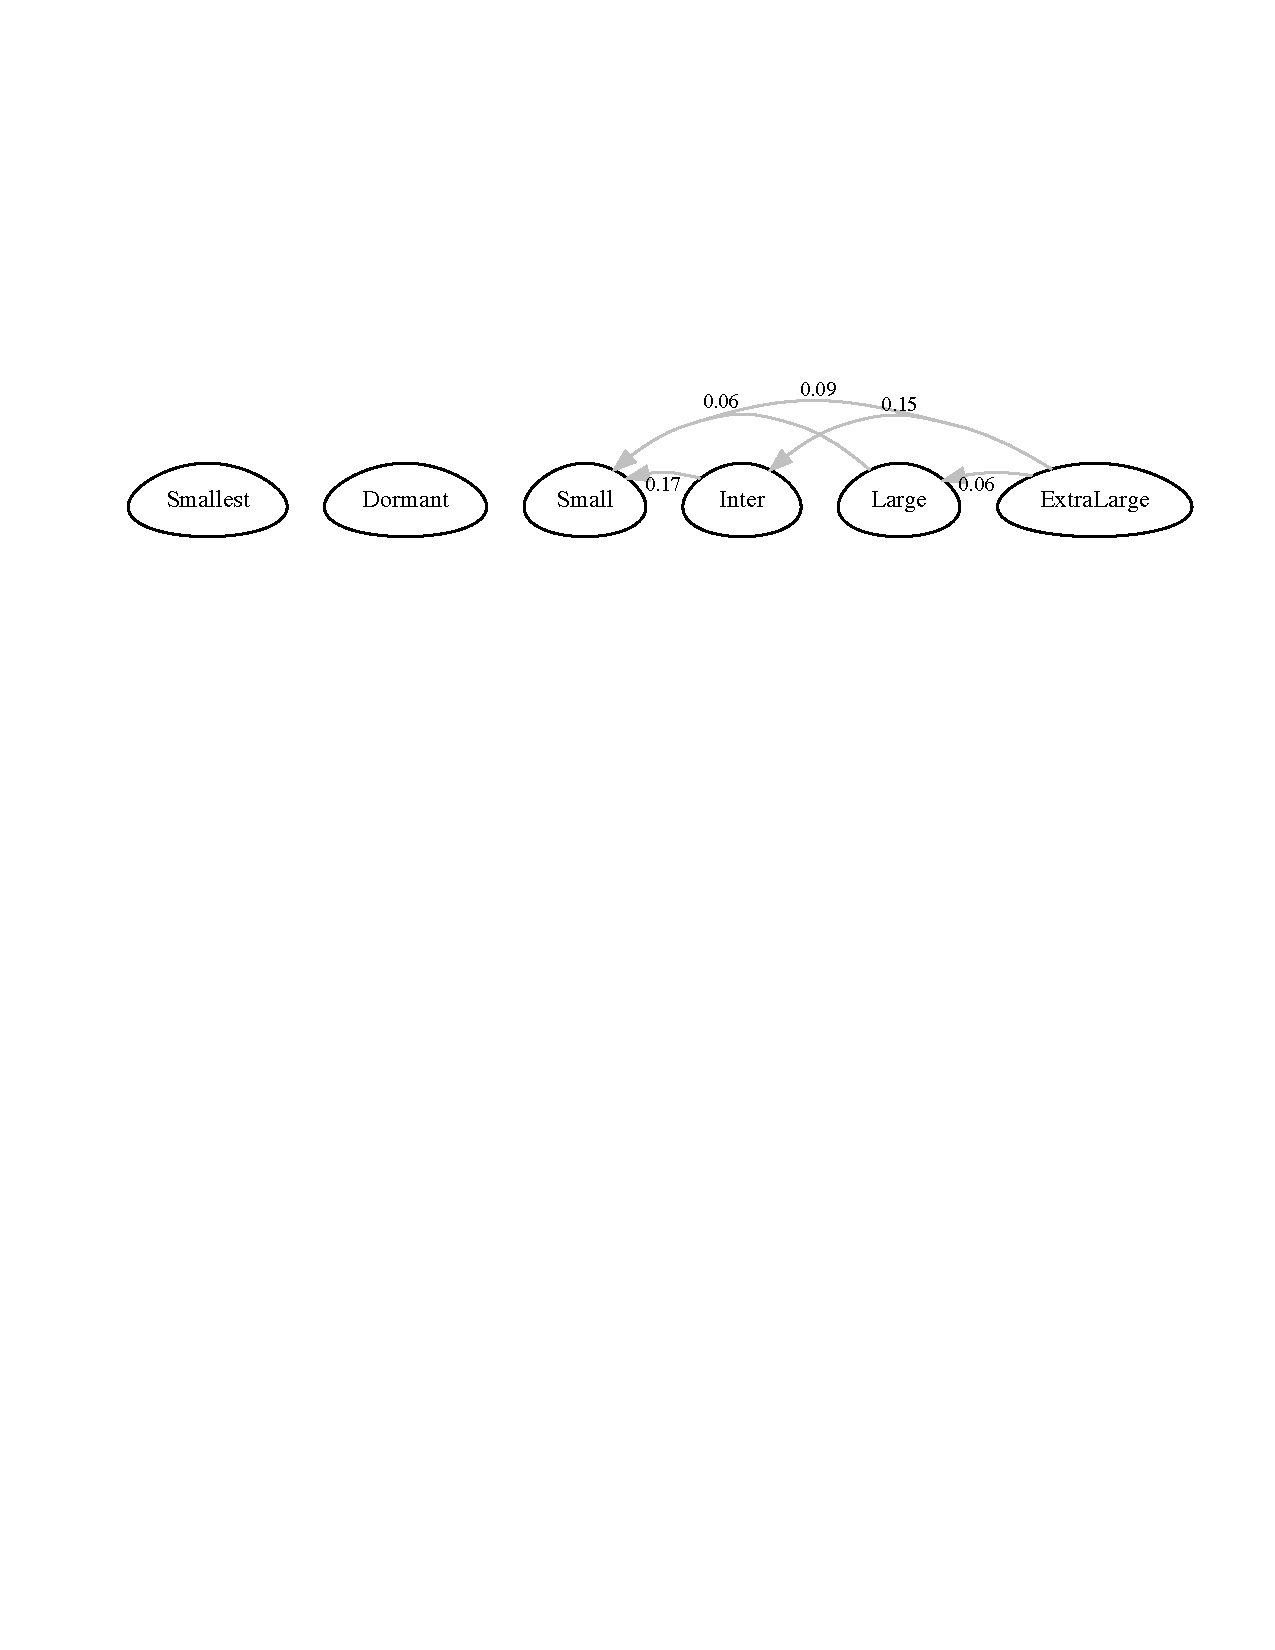
\includegraphics[keepaspectratio]{107-matU_matF_matC_files/figure-pdf/mat13-1.pdf}}

\begin{center}\rule{0.5\linewidth}{0.5pt}\end{center}

\subsection{Ejemplo de inclusión de matC en otras
familias}\label{ejemplo-de-inclusiuxf3n-de-matc-en-otras-familias}

\begin{center}\rule{0.5\linewidth}{0.5pt}\end{center}

\subsection{Clonación en otras
especies}\label{clonaciuxf3n-en-otras-especies}

Ver la lista de especies que incluyen la matriz de clonación,
\textbf{matC}. En esta lista vemos 825 filas, donde esto incluye las
poblaciones muestreadas donde matC \textgreater{} 0. Hay 108 especies
únicas donde la \textbf{matC} está incluida en la dinámica de la
población.

\begin{Shaded}
\begin{Highlighting}[]
\NormalTok{Clonal\_Species }\OtherTok{=}\NormalTok{ compadre }\SpecialCharTok{\%\textgreater{}\%}
  \FunctionTok{filter}\NormalTok{(clonality }\SpecialCharTok{\textgreater{}} \DecValTok{0}\NormalTok{) }\SpecialCharTok{\%\textgreater{}\%} \CommentTok{\# filtrar para aquellos con matC no nulo}
  \FunctionTok{select}\NormalTok{(mat, SpeciesAuthor, Family, clonality) }\SpecialCharTok{\%\textgreater{}\%} \CommentTok{\# seleccionar las columnas de interes}
  \FunctionTok{arrange}\NormalTok{(}\FunctionTok{desc}\NormalTok{(clonality)) }\CommentTok{\# ordenar por la columna de clonación}

\FunctionTok{head}\NormalTok{(Clonal\_Species) }\SpecialCharTok{|\textgreater{}} \FunctionTok{select}\NormalTok{(}\SpecialCharTok{{-}}\NormalTok{mat) }\SpecialCharTok{|\textgreater{}} \FunctionTok{flextable}\NormalTok{() }\CommentTok{\# ver las primeras 6 poblaciones}
\end{Highlighting}
\end{Shaded}

\begin{verbatim}
Error in `flextable()`:
! could not find function "flextable"
\end{verbatim}

\begin{center}\rule{0.5\linewidth}{0.5pt}\end{center}

\subsection{Cuantas familias de plantas incluyeron matriz de clonación
en sus
modelos}\label{cuantas-familias-de-plantas-incluyeron-matriz-de-clonaciuxf3n-en-sus-modelos}

Hay 44 familias de plantas donde la \textbf{matC} está incluida en la
dinámica.

\begin{Shaded}
\begin{Highlighting}[]
\CommentTok{\# Ver la lista de familias únicas con clonación}
\NormalTok{Families }\OtherTok{=}\NormalTok{ (}\FunctionTok{as.data.frame}\NormalTok{(}\FunctionTok{sort}\NormalTok{(}\FunctionTok{unique}\NormalTok{(Clonal\_Species}\SpecialCharTok{$}\NormalTok{Family))))}

\FunctionTok{head}\NormalTok{(Families) }\SpecialCharTok{|\textgreater{}} \FunctionTok{flextable}\NormalTok{() }\CommentTok{\# ver las primeras 6 familias}
\end{Highlighting}
\end{Shaded}

\begin{verbatim}
Error in `flextable()`:
! could not find function "flextable"
\end{verbatim}

\begin{center}\rule{0.5\linewidth}{0.5pt}\end{center}

\subsection{Clonación en las
Bromeliaceae}\label{clonaciuxf3n-en-las-bromeliaceae}

\begin{Shaded}
\begin{Highlighting}[]
\NormalTok{Bromeliaceae }\OtherTok{=}\NormalTok{ Clonal\_Species }\SpecialCharTok{\%\textgreater{}\%}
  \FunctionTok{filter}\NormalTok{(Family }\SpecialCharTok{==} \StringTok{"Bromeliaceae"}\NormalTok{) }\SpecialCharTok{\%\textgreater{}\%} \CommentTok{\# para la familia de bromelias}
  \FunctionTok{select}\NormalTok{(mat, SpeciesAuthor, Family, clonality) }\SpecialCharTok{\%\textgreater{}\%} \CommentTok{\# seleccionar las columnas de interés}
  \FunctionTok{arrange}\NormalTok{(}\FunctionTok{desc}\NormalTok{(clonality)) }\CommentTok{\# ordenar por la columna de clonación}

\NormalTok{Bromeliaceae}
\end{Highlighting}
\end{Shaded}

\begin{verbatim}
A COM(P)ADRE database ('CompadreDB') object with ?? SPECIES and 49 MATRICES.

# A tibble: 49 x 4
   mat        SpeciesAuthor           Family       clonality
   <list>     <chr>                   <chr>            <dbl>
 1 <CompdrMt> Tillandsia_brachycaulos Bromeliaceae      5.32
 2 <CompdrMt> Tillandsia_brachycaulos Bromeliaceae      5.04
 3 <CompdrMt> Tillandsia_brachycaulos Bromeliaceae      4.77
 4 <CompdrMt> Tillandsia_brachycaulos Bromeliaceae      3.94
 5 <CompdrMt> Aechmea_nudicaulis      Bromeliaceae      1.39
 6 <CompdrMt> Aechmea_nudicaulis      Bromeliaceae      1.26
 7 <CompdrMt> Aechmea_nudicaulis      Bromeliaceae      1.21
 8 <CompdrMt> Aechmea_nudicaulis      Bromeliaceae      1.20
 9 <CompdrMt> Aechmea_nudicaulis      Bromeliaceae      1.13
10 <CompdrMt> Aechmea_nudicaulis      Bromeliaceae      1.10
# i 39 more rows
\end{verbatim}

Seleccionamos una especie de bromelia, \emph{Aechmea nudicaulis}
(Sampaio, Picó \& Scarano, 2005), que tiene una matriz de clonación. En
este caso, la matriz de clonación es la \textbf{matC} y la matriz de
transición es la \textbf{matU}. La matriz de fecundidad no está incluida
en este modelo. Visualizamos la matriz de clonación y la matriz de
transición. En este caso, la matriz de clonación es la \textbf{matC} y
la matriz de transición es la \textbf{matU}. La matriz de fecundidad no
está incluida en este modelo.

\pandocbounded{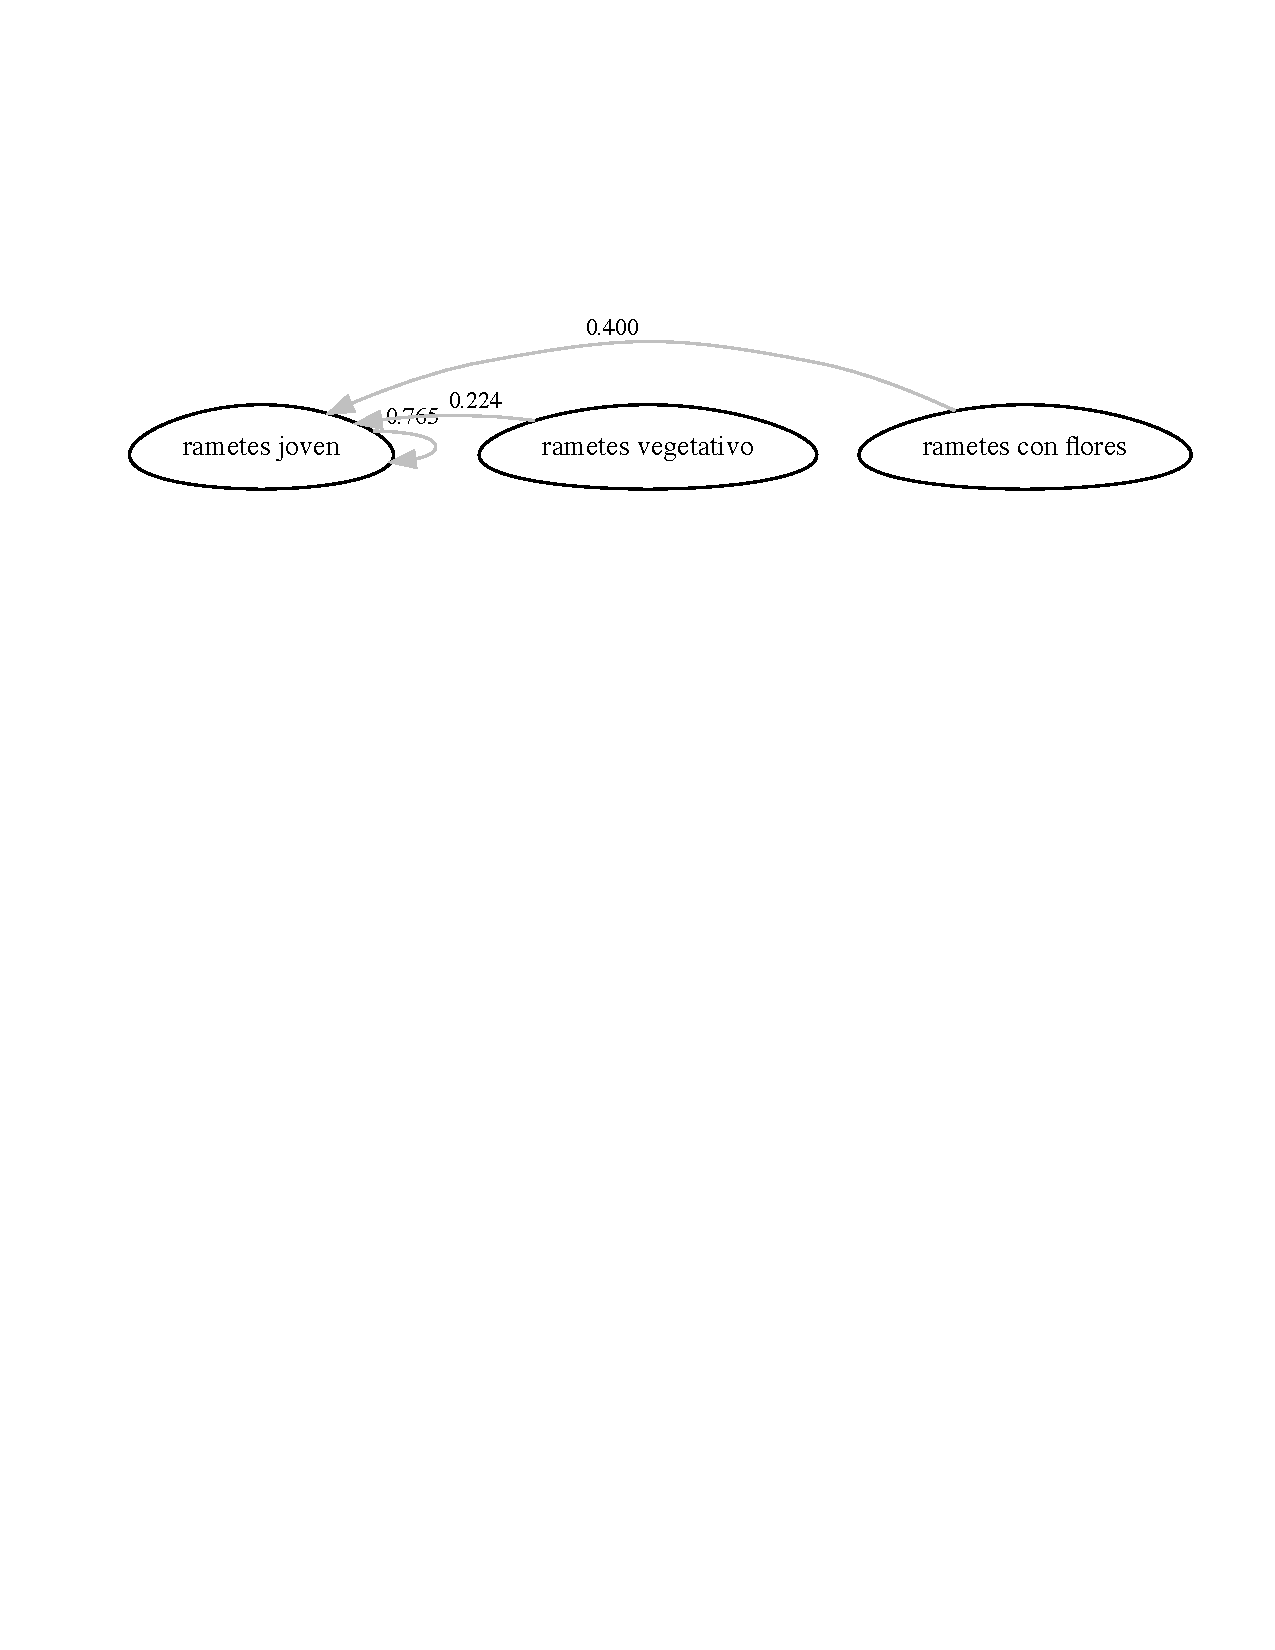
\includegraphics[keepaspectratio]{107-matU_matF_matC_files/figure-pdf/mat18-1.pdf}}

La dinámica de crecimiento clonal en la bromelia \emph{Aechmea
nudicaulis} (Sampaio, Picó \& Scarano, 2005) difiere de la observada en
\emph{Cypripedium calceolus}. En \emph{Aechmea nudicaulis}, la clonación
ocurre mediante la producción de hijuelos (offsets) que se separan de la
planta madre y se convierten en nuevos individuos. En cambio, en
\emph{Cypripedium calceolus}, la clonación se produce a través de
rizomas que permanecen conectados a la planta madre.

Sin embargo, en ambos casos surge la pregunta: \textbf{¿Cuándo hablamos
de crecimiento vegetativo y cuándo de clonación?}

En \emph{Cypripedium calceolus}, el aumento en tamaño y número de tallos
mediante rizomas no se considera clonación mientras permanezcan
conectados a la planta madre; solo se considera clonación cuando se
separan y se vuelven independientes. De manera similar, en \emph{Aechmea
nudicaulis}, la producción de hijuelos representa crecimiento vegetativo
hasta que estos se desprenden y se convierten en individuos autónomos.

Una revisión exhaustiva sobre este tema se encuentra en Cook (Cook,
1983) y Vallejo et al. (Vallejo-Marı́n, Dorken \& Barrett, 2010).

\begin{tcolorbox}[enhanced jigsaw, arc=.35mm, bottomrule=.15mm, bottomtitle=1mm, breakable, colback=white, colbacktitle=quarto-callout-tip-color!10!white, colframe=quarto-callout-tip-color-frame, coltitle=black, left=2mm, leftrule=.75mm, opacityback=0, opacitybacktitle=0.6, rightrule=.15mm, title=\textcolor{quarto-callout-tip-color}{\faLightbulb}\hspace{0.5em}{Recomendación}, titlerule=0mm, toprule=.15mm, toptitle=1mm]

\textbf{Regla práctica para distinguir crecimiento vegetativo de
clonaje.} Mientras los nuevos módulos (pseudobulbos, hijuelos, brotes de
rizoma) \textbf{permanezcan conectados} a la planta madre y compartan
recursos, se contabilizan como \textbf{crecimiento vegetativo} (van a
\texttt{matU} como permanencia o crecimiento entre estadios). Sólo
cuando se \textbf{separan físicamente} y se vuelven ecológicamente
independientes pasan a contabilizarse como \textbf{clonaje} (van a
\texttt{matC}). El criterio operativo es: ¿este módulo tiene un destino
demográfico independiente del resto?

\end{tcolorbox}

\subsection{Importancia de incluir clonación en modelos
poblacionales}\label{importancia-de-incluir-clonaciuxf3n-en-modelos-poblacionales}

\begin{tcolorbox}[enhanced jigsaw, arc=.35mm, bottomrule=.15mm, bottomtitle=1mm, breakable, colback=white, colbacktitle=quarto-callout-warning-color!10!white, colframe=quarto-callout-warning-color-frame, coltitle=black, left=2mm, leftrule=.75mm, opacityback=0, opacitybacktitle=0.6, rightrule=.15mm, title=\textcolor{quarto-callout-warning-color}{\faExclamationTriangle}\hspace{0.5em}{Advertencia}, titlerule=0mm, toprule=.15mm, toptitle=1mm]

\textbf{La mayoría de los modelos poblacionales de especies clonales
omiten \texttt{matC}.} Janovsky et al. (Janovskỳ, Herben \& Klimešová,
2017) muestran que en COMPADRE la mayoría de las especies con
reproducción clonal documentada \textbf{no} reportan una matriz
\texttt{matC}, y muchos artículos que reconocen el clonaje como un
proceso importante tampoco lo incorporan formalmente al modelo. Esta
omisión sesga las estimaciones de λ, oculta el efecto del clonaje sobre
la diversidad genética, y limita análisis posteriores de selección y
deriva.

\end{tcolorbox}

Janovsky et al. (Janovskỳ, Herben \& Klimešová, 2017) destacan la
relevancia de la clonación en el crecimiento y la dinámica poblacional.
Al analizar la base de datos COMPADRE, encontraron que la mayoría de las
especies con clonación no incluyen una matriz matC, y que muchos
estudios que reconocen la clonación como factor importante tampoco la
incorporan en sus modelos.

Esta omisión es preocupante, ya que la clonación puede:

\begin{itemize}
\tightlist
\item
  Alterar la estructura genética de las poblaciones.
\item
  Reducir la diversidad genética.
\item
  Influir en la adaptación a cambios ambientales.
\end{itemize}

Por lo tanto, es crucial integrar la clonación en los modelos de
dinámica poblacional y en estudios evolutivos cuando esté presente.

\bookmarksetup{startatroot}

\chapter{Acercamiento bayesiano para calcular transiciones y
fecundidades}\label{acercamiento-bayesiano-para-calcular-transiciones-y-fecundidades}

Por: Raymond L. Tremblay

Los modelos poblacionales bayesianos permiten integrar explícitamente la
incertidumbre demográfica, de muestreo y de proceso en el análisis de la
dinámica poblacional. Este capítulo introduce los modelos de proyección
poblacional bayesianos (Bayesian MPP) como una extensión coherente de
los modelos matriciales clásicos.

\section{Modelos de proyección poblacional bayesianos: integrar
incertidumbre y
proceso}\label{modelos-de-proyecciuxf3n-poblacional-bayesianos-integrar-incertidumbre-y-proceso}

Los modelos de proyección poblacional bayesianos (Bayesian Population
Projection Models, MPP) extienden los modelos matriciales tradicionales
al tratar los parámetros vitales (supervivencia, crecimiento y
fecundidad) como variables aleatorias en lugar de valores puntuales
fijos. Esta formulación permite propagar explícitamente la incertidumbre
desde los datos primarios hasta las proyecciones de abundancia y
crecimiento poblacional (λ), algo fundamental en poblaciones con tamaños
de muestra reducidos, series temporales cortas o alta variabilidad
ambiental.

En este capítulo se presenta el marco conceptual de los Bayesian MPP,
mostrando cómo se combinan modelos de observación y proceso dentro de
una jerarquía bayesiana para estimar matrices poblacionales con
distribuciones posteriores completas. Se discuten las ventajas clave de
este enfoque frente a métodos frecuentistas, incluyendo la incorporación
de información previa, el manejo coherente de datos faltantes y la
cuantificación directa de la incertidumbre en predicciones a corto y
largo plazo.

A través de ejemplos aplicados, se ilustra cómo los Bayesian MPP
facilitan la evaluación del riesgo poblacional, la comparación entre
escenarios de manejo y la integración posterior con análisis de
elasticidad, sensibilidad y LTRE. Este capítulo se diferencia de los
anteriores porque desplaza el énfasis desde la estimación puntual de
parámetros hacia la inferencia probabilística completa de la dinámica
poblacional, un enfoque especialmente relevante en biología de la
conservación y ecología aplicada.

\begin{Shaded}
\begin{Highlighting}[]
\ControlFlowTok{if}\NormalTok{ (}\SpecialCharTok{!}\FunctionTok{require}\NormalTok{(}\StringTok{"pacman"}\NormalTok{)) }\FunctionTok{install.packages}\NormalTok{(}\StringTok{"pacman"}\NormalTok{)}
\NormalTok{pacman}\SpecialCharTok{::}\FunctionTok{p\_load}\NormalTok{(janitor, tidyverse)}

\FunctionTok{library}\NormalTok{(tidyverse)}
\FunctionTok{library}\NormalTok{(janitor)}
\FunctionTok{library}\NormalTok{(popbio) }\CommentTok{\# para la función projection.matrix()}
\FunctionTok{library}\NormalTok{(raretrans) }\CommentTok{\# disponible en CRAN: install.packages("raretrans")}
\FunctionTok{library}\NormalTok{(DiagrammeR)}
\FunctionTok{library}\NormalTok{(Rage)}
\FunctionTok{library}\NormalTok{(flextable)}
\end{Highlighting}
\end{Shaded}

\begin{Shaded}
\begin{Highlighting}[]
\NormalTok{rlt\_theme }\OtherTok{\textless{}{-}} \FunctionTok{theme}\NormalTok{(}
  \AttributeTok{axis.title.y =} \FunctionTok{element\_text}\NormalTok{(}\AttributeTok{colour =} \StringTok{"grey20"}\NormalTok{, }\AttributeTok{size =} \DecValTok{10}\NormalTok{, }\AttributeTok{face =} \StringTok{"bold"}\NormalTok{),}
  \AttributeTok{axis.text.x =} \FunctionTok{element\_text}\NormalTok{(}\AttributeTok{colour =} \StringTok{"grey20"}\NormalTok{, }\AttributeTok{size =} \DecValTok{10}\NormalTok{, }\AttributeTok{face =} \StringTok{"bold"}\NormalTok{),}
  \AttributeTok{axis.text.y =} \FunctionTok{element\_text}\NormalTok{(}\AttributeTok{colour =} \StringTok{"grey20"}\NormalTok{, }\AttributeTok{size =} \DecValTok{15}\NormalTok{, }\AttributeTok{face =} \StringTok{"bold"}\NormalTok{),}
  \AttributeTok{axis.title.x =} \FunctionTok{element\_text}\NormalTok{(}\AttributeTok{colour =} \StringTok{"grey20"}\NormalTok{, }\AttributeTok{size =} \DecValTok{15}\NormalTok{, }\AttributeTok{face =} \StringTok{"bold"}\NormalTok{)}
\NormalTok{) }\SpecialCharTok{+}
  \FunctionTok{theme}\NormalTok{(}
    \CommentTok{\# Remover los bordes}
    \AttributeTok{panel.border =} \FunctionTok{element\_blank}\NormalTok{(),}
    \CommentTok{\# Remover las líneas}
    \AttributeTok{panel.grid.major =} \FunctionTok{element\_blank}\NormalTok{(),}
    \AttributeTok{panel.grid.minor =} \FunctionTok{element\_blank}\NormalTok{(),}
    \CommentTok{\# Remover el fondo del panel}
    \AttributeTok{panel.background =} \FunctionTok{element\_blank}\NormalTok{(),}
    \CommentTok{\# añadir lineas más gruesas}
    \AttributeTok{axis.line.x =} \FunctionTok{element\_line}\NormalTok{(}\AttributeTok{colour =} \StringTok{"black"}\NormalTok{, }\AttributeTok{linewidth =} \DecValTok{1}\NormalTok{),}
    \AttributeTok{axis.line.y =} \FunctionTok{element\_line}\NormalTok{(}\AttributeTok{colour =} \StringTok{"black"}\NormalTok{, }\AttributeTok{linewidth =} \DecValTok{1}\NormalTok{)}
\NormalTok{  )}

\NormalTok{diverging}\OtherTok{=} \FunctionTok{c}\NormalTok{(}\StringTok{"\#009392"}\NormalTok{,}\StringTok{"\#CF597E"}\NormalTok{,}\StringTok{"\#E9E29C"}\NormalTok{, }\StringTok{"\#39B185"}\NormalTok{,}\StringTok{"\#EEB479"}\NormalTok{ , }\StringTok{"\#9CCB86"}\NormalTok{ )}

\CommentTok{\# {-}{-}{-} 2. Combinarlos en un objeto de tipo lista {-}{-}{-}}
\CommentTok{\# Esta lista se puede añadir al gráfico con un solo \textquotesingle{}+\textquotesingle{}}
\NormalTok{rlt\_style\_fill }\OtherTok{\textless{}{-}} \ControlFlowTok{function}\NormalTok{() \{}
  \FunctionTok{list}\NormalTok{(}
\NormalTok{    rlt\_theme,}
    \FunctionTok{scale\_fill\_manual}\NormalTok{(}\AttributeTok{values =}\NormalTok{ diverging)}
\NormalTok{  )}
\NormalTok{\}}

\NormalTok{rlt\_style\_colour }\OtherTok{\textless{}{-}} \ControlFlowTok{function}\NormalTok{() \{}
  \FunctionTok{list}\NormalTok{(}
\NormalTok{    rlt\_theme,}
    \FunctionTok{scale\_colour\_manual}\NormalTok{(}\AttributeTok{values =}\NormalTok{ diverging)}
\NormalTok{  )}
\NormalTok{\}}
\end{Highlighting}
\end{Shaded}

\section{¿Qué es un análisis bayesiano? Una introducción
rápida}\label{quuxe9-es-un-anuxe1lisis-bayesiano-una-introducciuxf3n-ruxe1pida}

En estadística clásica (frecuentista), tratamos los parámetros (e.g., la
probabilidad de transición de plántula a juvenil) como \textbf{valores
fijos pero desconocidos}, y los datos como variables aleatorias. La
inferencia consiste en estimar el parámetro a partir de los datos: si
observamos 2 transiciones de 7 plántulas, el estimador puntual es 2/7 =
0.286, sin más información.

En el marco bayesiano, invertimos la perspectiva: los \textbf{datos son
lo que observamos}, y los \textbf{parámetros se tratan como variables
aleatorias} sobre las que tenemos creencias. Esas creencias se expresan
como una \textbf{distribución previa} (lo que sabíamos antes de mirar
los datos) y se actualizan a una \textbf{distribución posterior} (lo que
sabemos después). La regla de actualización es la fórmula de Bayes:

\[\underbrace{P(\theta \mid \text{datos})}_{\text{posterior}} \propto \underbrace{P(\text{datos} \mid \theta)}_{\text{verosimilitud}} \times \underbrace{P(\theta)}_{\text{previa}}\]

En español plano: la posterior es proporcional a la previa multiplicada
por la verosimilitud. La previa aporta información cuando los datos son
escasos; la verosimilitud (los datos) domina cuando hay muchas
observaciones. \textbf{Esta propiedad es exactamente lo que necesitamos
para especies raras}: si observamos 2 plántulas y 0 transiciones a
juvenil, el estimador frecuentista da \(\hat{p} = 0\) (lo cual implica
imposibilidad biológica), mientras que el estimador bayesiano combina
las 2 observaciones con la previa y da una probabilidad pequeña pero
positiva, con incertidumbre cuantificada.

\begin{tcolorbox}[enhanced jigsaw, arc=.35mm, bottomrule=.15mm, bottomtitle=1mm, breakable, colback=white, colbacktitle=quarto-callout-note-color!10!white, colframe=quarto-callout-note-color-frame, coltitle=black, left=2mm, leftrule=.75mm, opacityback=0, opacitybacktitle=0.6, rightrule=.15mm, title=\textcolor{quarto-callout-note-color}{\faInfo}\hspace{0.5em}{Nota}, titlerule=0mm, toprule=.15mm, toptitle=1mm]

\textbf{La regla de Bayes en lenguaje cotidiano.}

\[\text{Lo que crees ahora} \;\propto\; \text{Lo que creías antes} \;\times\; \text{Lo que dicen los datos}\]

Cuando los datos son muchos y consistentes, dominan: la posterior se
parece a la verosimilitud. Cuando los datos son escasos o ambiguos, la
previa importa: la posterior se parece a la previa. El método bayesiano
hace este equilibrio explícito y reproducible.

\end{tcolorbox}

\begin{tcolorbox}[enhanced jigsaw, arc=.35mm, bottomrule=.15mm, bottomtitle=1mm, breakable, colback=white, colbacktitle=quarto-callout-tip-color!10!white, colframe=quarto-callout-tip-color-frame, coltitle=black, left=2mm, leftrule=.75mm, opacityback=0, opacitybacktitle=0.6, rightrule=.15mm, title=\textcolor{quarto-callout-tip-color}{\faLightbulb}\hspace{0.5em}{Recomendación}, titlerule=0mm, toprule=.15mm, toptitle=1mm]

\textbf{Por qué leer este capítulo (incluso si nunca has hecho un
análisis bayesiano).} La estimación clásica de matrices de transición
---\texttt{projection.matrix()}--- es perfectamente adecuada cuando el
tamaño de muestra es grande y cada transición se observó muchas veces.
Pero en estudios reales de orquídeas, casi nunca es así: las muestras
son pequeñas, varias transiciones tienen 0 observaciones, y el resultado
es una matriz con ceros que la biología sabe que no son cero. El enfoque
bayesiano resuelve esto sin ``inventar'' datos: usa explícitamente lo
que ya sabes sobre el ciclo de vida (la previa) y produce estimaciones
realistas con intervalos de credibilidad. Aprender a usarlo es una de
las inversiones de mayor retorno en la dinámica poblacional aplicada.

\end{tcolorbox}

\section{Introducción al MPP
Bayesiano}\label{introducciuxf3n-al-mpp-bayesiano}

Este capítulo presenta una alternativa bayesiana para estimar los
parámetros de las matrices de transición y fecundidad en modelos
poblacionales, especialmente útil en el estudio de especies raras. Estas
especies suelen tener tamaños de muestra reducidos o transiciones
vitales poco frecuentes, lo que dificulta obtener estimaciones
confiables. El enfoque bayesiano propuesto permite incorporar
conocimiento previo sobre el ciclo de vida de la especie para generar
estimaciones más realistas.

\subsection{Ejemplo de especie con tres
etapas}\label{ejemplo-de-especie-con-tres-etapas}

Consideremos una especie hipotética con tres etapas en su ciclo de vida:
semillas, plántulas y adultos. En este caso, sólo los adultos producen
semillas. El primer paso del análisis consiste en identificar qué etapas
tienen mayor influencia en la dinámica poblacional y cómo optimizar la
recolección de datos en campo.

La primera figura muestra el ciclo de vida considerado. Tras definirlo,
se recolectaron datos de campo y se estimaron las tasas de transición y
fecundidad. Los resultados revelaron lo siguiente:

\begin{enumerate}
\def\labelenumi{\arabic{enumi}.}
\tightlist
\item
  \textbf{No se observaron semillas}. Esto podría indicar que todas
  germinaron y pasaron a la etapa de plántula.
\end{enumerate}

\begin{itemize}
\tightlist
\item
  ¿Es realista asumir que el 100\% de las semillas germinaron?
\item
  ¿Por qué no se encontraron semillas en el muestreo?
\end{itemize}

\begin{enumerate}
\def\labelenumi{\arabic{enumi}.}
\setcounter{enumi}{1}
\tightlist
\item
  \textbf{No se observaron plántulas}. Esto podría interpretarse como
  que todas murieron o que ninguna semilla germinó.
\end{enumerate}

\begin{itemize}
\tightlist
\item
  ¿Es realista asumir que todas las plántulas mueren durante el ciclo de
  vida de una especie?
\end{itemize}

Estas interpretaciones extremas ---que ningún individuo muere o que
todos mueren--- no son biológicamente realistas. Sin embargo, pueden
surgir como resultado de un tamaño de muestra reducido. Por ejemplo, si
sólo se observaron 4 plantas adultas (debido a que la especie es rara) y
todas sobrevivieron, se estimaría una tasa de supervivencia del 100\%,
lo que implicaría que los individuos son ``inmortales''. Este resultado
no refleja la realidad biológica, sino una limitación del muestreo: por
simple azar, no se observó ninguna muerte. Por lo tanto, es fundamental
reconocer cuándo los parámetros estimados no representan adecuadamente
la historia de vida típica de la especie.

\subsection{\texorpdfstring{El papel del paquete
\texttt{raretrans}}{El papel del paquete raretrans}}\label{el-papel-del-paquete-raretrans}

El paquete \texttt{raretrans} fue desarrollado para abordar este tipo de
situaciones. Utiliza un enfoque bayesiano que permite incorporar
conocimiento previo sobre el ciclo de vida de la especie, ayudando a
estimar parámetros más realistas incluso cuando los datos son escasos o
incompletos.

\subsection{Ejemplos de interpretaciones no
realistas}\label{ejemplos-de-interpretaciones-no-realistas}

Algunas interpretaciones biológicamente poco plausibles que pueden
surgir del análisis de datos limitados incluyen:

\begin{itemize}
\tightlist
\item
  Todas las semillas germinan y se convierten en plántulas.
\item
  Ninguna plántula sobrevive ni alcanza la etapa adulta.
\item
  Todos los adultos sobreviven sin mortalidad.
\item
  Ningún adulto produce semillas.
\end{itemize}

\textbf{Nota}: Aunque estos resultados pueden surgir directamente de los
datos recolectados, muchas veces son consecuencia de tamaños de muestra
pequeños o de eventos raros que no se observaron durante el periodo de
muestreo. Por ello, es esencial considerar tanto la biología de la
especie como las limitaciones del muestreo al interpretar los datos.

\begin{Shaded}
\begin{Highlighting}[]
\NormalTok{matA }\OtherTok{\textless{}{-}} \FunctionTok{rbind}\NormalTok{(}
  \FunctionTok{c}\NormalTok{(}\FloatTok{0.0}\NormalTok{, }\FloatTok{0.0}\NormalTok{, }\FloatTok{0.0}\NormalTok{),}
  \FunctionTok{c}\NormalTok{(}\FloatTok{1.0}\NormalTok{, }\FloatTok{0.0}\NormalTok{, }\FloatTok{0.0}\NormalTok{),}
  \FunctionTok{c}\NormalTok{(}\FloatTok{0.0}\NormalTok{, }\FloatTok{0.0}\NormalTok{, }\FloatTok{0.9}\NormalTok{)}
\NormalTok{)}
\NormalTok{stages }\OtherTok{\textless{}{-}} \FunctionTok{c}\NormalTok{(}\StringTok{"semillas"}\NormalTok{, }\StringTok{"plantulas"}\NormalTok{, }\StringTok{"adultos"}\NormalTok{)}
\NormalTok{title }\OtherTok{\textless{}{-}} \ConstantTok{NULL}
\end{Highlighting}
\end{Shaded}

\section{Evaluación crítica del ciclo de vida y la matriz
poblacional}\label{evaluaciuxf3n-cruxedtica-del-ciclo-de-vida-y-la-matriz-poblacional}

El ciclo de vida propuesto para esta especie hipotética presenta
limitaciones importantes que lo hacen poco realista. En particular:

\begin{itemize}
\tightlist
\item
  No se observaron semillas en el muestreo, lo que sugiere que todas
  germinaron y pasaron a la etapa de plántula. Sin embargo, asumir una
  germinación del 100\% es altamente improbable en condiciones
  naturales.
\item
  Ninguna plántula sobrevivió, lo que indica una falla completa en la
  transición hacia la etapa adulta.
\end{itemize}

Como resultado, la tasa de crecimiento poblacional asintótica observada
es \(\lambda = 0.9\) lo que implica una población en declive.

Además, la matriz poblacional estimada presenta dos propiedades
estructurales problemáticas:

\begin{enumerate}
\def\labelenumi{\arabic{enumi}.}
\item
  \textbf{No es ergódica}: No es posible transitar desde cualquier
  estado a cualquier otro estado dentro del ciclo de vida. Esto limita
  la conectividad entre etapas y reduce la capacidad de la matriz para
  representar adecuadamente la dinámica poblacional.
\item
  \textbf{Es reducible}: Una o más filas y columnas pueden eliminarse
  sin alterar las propiedades fundamentales de la matriz (como sus
  eigenvalores y eigenvectores). Esto indica que ciertas etapas del
  ciclo de vida no contribuyen significativamente a la dinámica
  poblacional, lo cual puede ser un artefacto del muestreo o de una
  estructura biológica mal representada.
\end{enumerate}

\begin{Shaded}
\begin{Highlighting}[]
\FunctionTok{plot\_life\_cycle}\NormalTok{(matA, }\AttributeTok{stages =}\NormalTok{ stages)}
\end{Highlighting}
\end{Shaded}

\pandocbounded{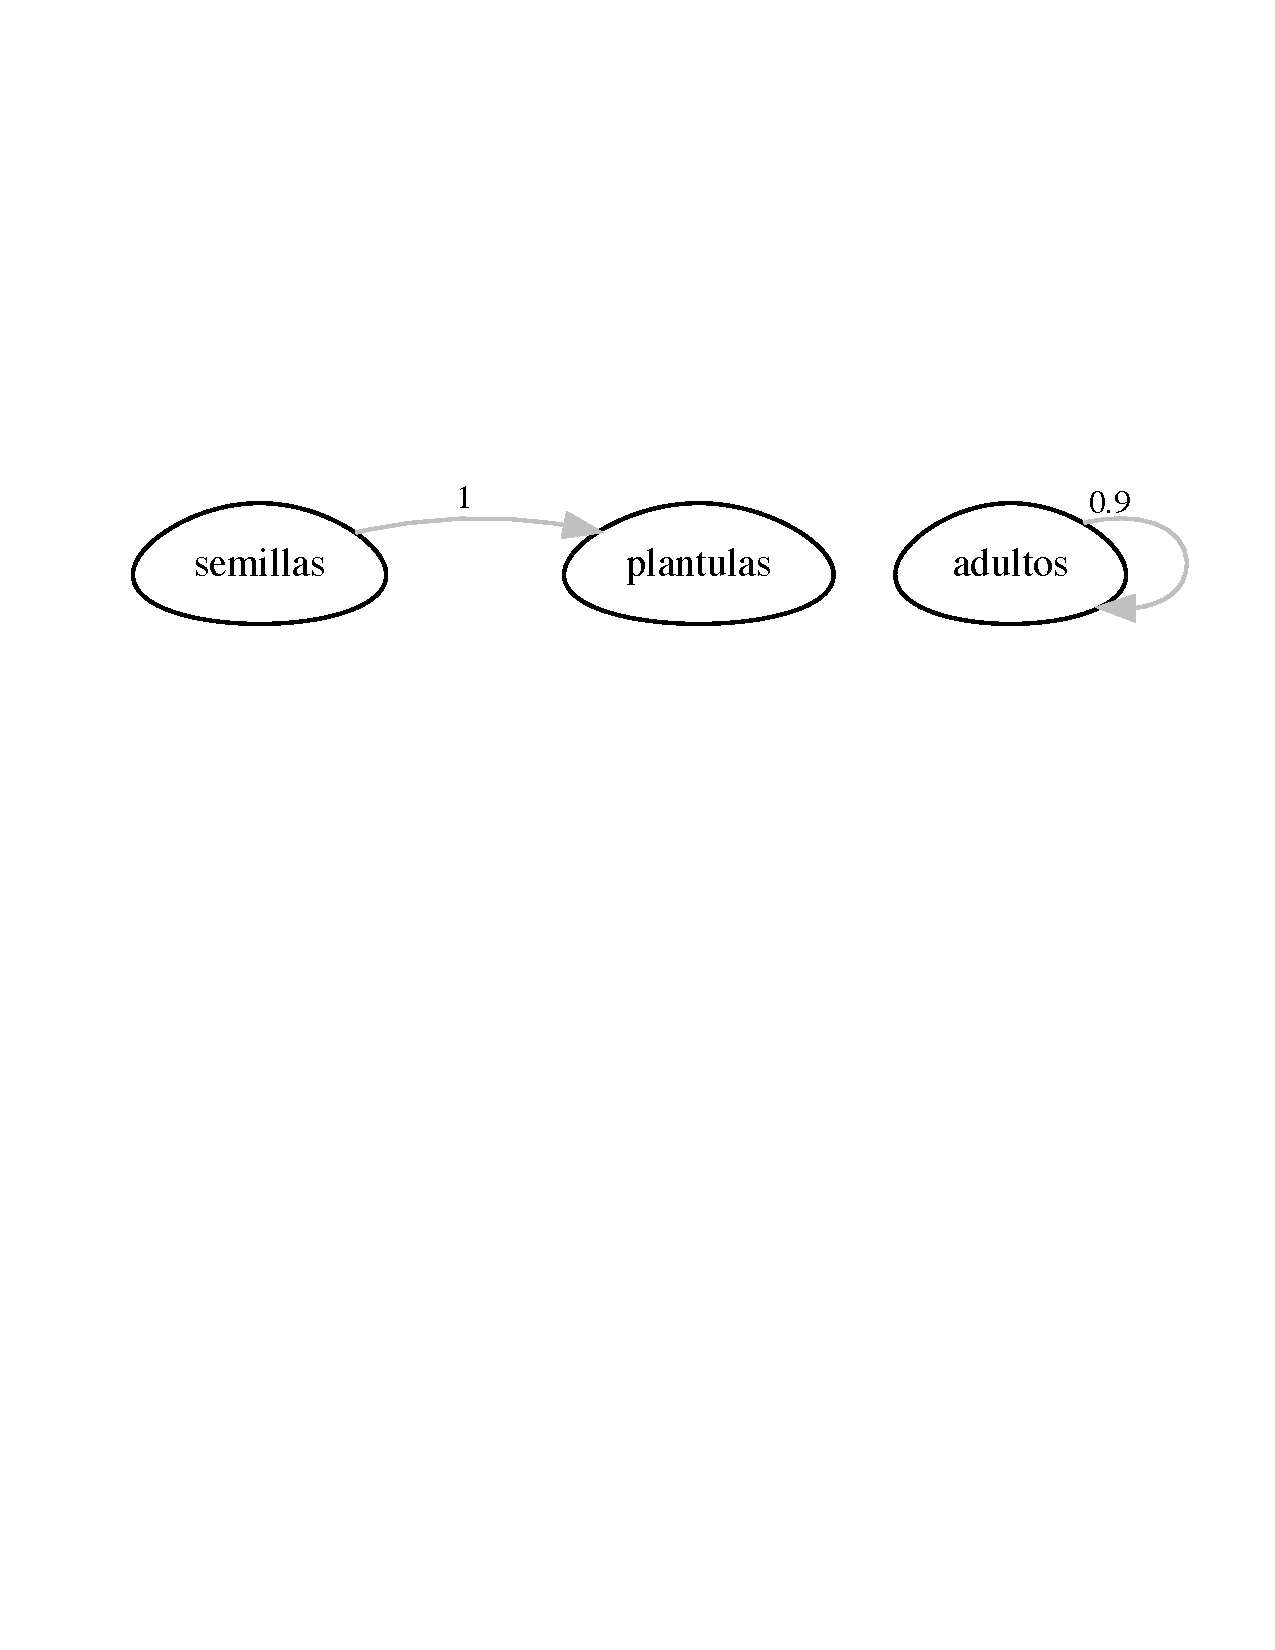
\includegraphics[keepaspectratio]{108-Bayesian_PPM_files/figure-pdf/bayes2-1.pdf}}

\subsection{Interpretaciones biológicamente irreales de los datos
existentes}\label{interpretaciones-bioluxf3gicamente-irreales-de-los-datos-existentes}

Al estudiar especies longevas como \emph{Sequoia sempervirens}, es común
enfrentar interpretaciones erróneas derivadas de datos limitados o mal
contextualizados. Esta especie puede alcanzar tamaños extraordinarios
(diámetros a la altura del pecho, \emph{dbh}, mayores a 3 metros) y
tener una longevidad estimada entre 1,200 y 2,200 años.

Supongamos que se realiza un muestreo de más de 1,000 individuos
grandes. Es posible que, en un intervalo de uno o incluso diez años, no
se observe la muerte de ningún individuo. A partir de estos datos, se
podría concluir erróneamente que la supervivencia anual es del 100\%.
Sin embargo, esta interpretación es biológicamente poco realista por
varias razones:

\begin{enumerate}
\def\labelenumi{\arabic{enumi}.}
\item
  \textbf{Tamaño de muestra insuficiente}: Si el muestreo se ampliara a
  10,000 o 100,000 individuos, probablemente se detectarían muertes,
  aunque fueran pocas. Esto sugiere que la mortalidad es baja, pero no
  nula.
\item
  \textbf{Relación entre tamaño y mortalidad}: En plantas, la
  probabilidad de morir suele disminuir con el tamaño del individuo. Los
  árboles más grandes tienen mayor resistencia a factores ambientales y
  biológicos, lo que reduce su tasa de mortalidad.
\item
  \textbf{Dependencia temporal de la mortalidad}: La muerte de
  individuos puede estar influenciada por eventos bióticos (plagas,
  enfermedades) o abióticos (sequías, incendios, tormentas) que varían
  entre años. En años extremos, la mortalidad puede aumentar
  significativamente.
\end{enumerate}

Por lo tanto, aunque los datos observados sugieren una supervivencia
perfecta, la probabilidad real de mortalidad es baja pero no cero. Este
tipo de sesgo en la interpretación puede ser corregido mediante enfoques
estadísticos más robustos, como el uso de modelos bayesianos que
incorporan incertidumbre y conocimiento previo sobre la biología de la
especie.

\begin{center}\rule{0.5\linewidth}{0.5pt}\end{center}

\section{\texorpdfstring{El paquete
\texttt{raretrans}}{El paquete raretrans}}\label{el-paquete-raretrans}

En la siguiente sección usaremos el paquete \texttt{raretrans}, que
facilita los estimados de las entradas en las matrices de transición y
fecundidades. El manuscrito (Tremblay et~al., 2021; Tyre, Tremblay \&
Perez, 2024) contiene los datos originales y el uso del paquete. Para
tener acceso a los documentos sigan el siguiente enlace:
\url{https://doi.org/10.1016/j.ecolmodel.2021.109526}.

\textbf{Population projections from holey matrices: Using prior
information to estimate rare transition events}

Resumen

Las matrices de proyección poblacional (MPP) son una herramienta común
para predecir el comportamiento de la población a corto y largo plazo.
Sin embargo, cuando se utilizan para especies raras, amenazadas y en
peligro de extinción los datos disponibles suelen tener tamaños de
muestra reducido. En consecuencia, algunos eventos demográficos podrían
perderse en la modelización dando como resultado matrices con eventos
faltantes que reflejen trayectorias de ciclo de vida incompletas o
biológicamente poco realistas. Estas matrices con eventos faltantes
(ceros; e.g., sin observación de semillas que se transforman en
plántulas) a menudo se sustituyen utilizando información de la
literatura aunque información referente a otras poblaciones, otros
períodos de tiempo, otras especies usualmente se omite.

Una forma de abordar este problema es a través de métodos bayesianos
para el ajuste de los parámetros matriciales. Este marco estadístico nos
permite usar información previa para completar los valores faltantes
usando, por ejemplo, una distribución de Dirichlet para incluir
información sobre las transiciones de estado y una distribución Gamma
como previa para la fecundidad. Este método permite integrar información
conocida (\emph{a priori}) e incluir explícitamente el peso de la
información previa en las distribuciones posteriores. Además, al
establecer explícitamente las distribuciones previas, los resultados son
reproducibles y se pueden volver a evaluar con diferentes distribuciones
\emph{a priori} en el futuro. A continuación mostramos cómo el uso de
estos métodos en datos reales influye en la dispersión de los resultados
posteriores y origina matrices irreducibles y ergódicas, permitiendo
hacer inferencias biológicamente más realistas sobre las probabilidades
de transición y fecundidad.

\section{Instalación del paquete
raretrans}\label{instalaciuxf3n-del-paquete-raretrans}

El paquete \texttt{raretrans} ya está disponible en CRAN, por lo que se
puede instalar de la manera habitual. Solo es necesario ejecutar la
instrucción una vez; en ejecuciones posteriores basta con cargar la
biblioteca con \texttt{library(raretrans)}.

\begin{Shaded}
\begin{Highlighting}[]
\CommentTok{\# Instalar desde CRAN (ejecutar solo una vez)}
\FunctionTok{install.packages}\NormalTok{(}\StringTok{"raretrans"}\NormalTok{)}
\end{Highlighting}
\end{Shaded}

\begin{Shaded}
\begin{Highlighting}[]
\FunctionTok{library}\NormalTok{(raretrans)}
\end{Highlighting}
\end{Shaded}

Ver el siguiente enlace para más información, la información que se
presenta a continuación es una traducción y ampliación de la información
del siguiente enlace. A continuación se muestra el uso del paquete
\texttt{raretrans} para estimar los parámetros en una población y en un
periodo de transición determinados.

\url{https://atyre2.github.io/raretrans/articles/onepopperiod.html}

A continuación se ejemplifica el uso del paquete \texttt{raretrans} para
estimar los parámetros en una población y en un periodo de transición
determinados.

\begin{Shaded}
\begin{Highlighting}[]
\CommentTok{\# Mi tema de formato de las gráficas de ggplot2 personal}
\NormalTok{rlt\_theme }\OtherTok{\textless{}{-}} \FunctionTok{theme}\NormalTok{(}\AttributeTok{axis.title.y =} \FunctionTok{element\_text}\NormalTok{(}\AttributeTok{colour=}\StringTok{"grey20"}\NormalTok{,}\AttributeTok{size=}\DecValTok{15}\NormalTok{,}\AttributeTok{face=}\StringTok{"bold"}\NormalTok{),}
        \AttributeTok{axis.text.x =} \FunctionTok{element\_text}\NormalTok{(}\AttributeTok{colour=}\StringTok{"grey20"}\NormalTok{,}\AttributeTok{size=}\DecValTok{15}\NormalTok{, }\AttributeTok{face=}\StringTok{"bold"}\NormalTok{),}
        \AttributeTok{axis.text.y =} \FunctionTok{element\_text}\NormalTok{(}\AttributeTok{colour=}\StringTok{"grey20"}\NormalTok{,}\AttributeTok{size=}\DecValTok{15}\NormalTok{,}\AttributeTok{face=}\StringTok{"bold"}\NormalTok{),  }
        \AttributeTok{axis.title.x =} \FunctionTok{element\_text}\NormalTok{(}\AttributeTok{colour=}\StringTok{"grey20"}\NormalTok{,}\AttributeTok{size=}\DecValTok{15}\NormalTok{,}\AttributeTok{face=}\StringTok{"bold"}\NormalTok{))}
\end{Highlighting}
\end{Shaded}

\section{Obtención de la matriz de
proyección}\label{obtenciuxf3n-de-la-matriz-de-proyecciuxf3n}

\texttt{raretrans} supone que la matriz de proyección es una lista con
dos componentes:

\begin{itemize}
\item
  \textbf{Matriz de transición}: Probabilidades de pasar de una etapa a
  otra (o permanecer en la misma).
\item
  \textbf{Matriz de fecundidad}: Número de nuevos individuos producidos
  por cada etapa reproductiva.
\end{itemize}

Este es el formato de salida de \texttt{popbio::projection.matrix}. Si
tenemos transiciones individuales en nuestra base de datos (con clase
\texttt{data.frame()}), podemos usar
\texttt{raretrans::get\_state\_vector} para obtener el número inicial de
individuos por etapa.

Podemos utilizar la función \texttt{popbio::projection.matrix} para
obtener los datos necesarios. Hacemos una demostración con los datos de
transición y fecundidad de \emph{Lepanthes eltoroensis} \textbf{POPNUM
250} en el \textbf{periodo 5}. \emph{Lepanthes eltoroensis} es una
orquídea epífita, endémica de Puerto Rico y con una distribución
limitada a una pequeña región de la isla.

\begin{figure}[H]

{\centering \pandocbounded{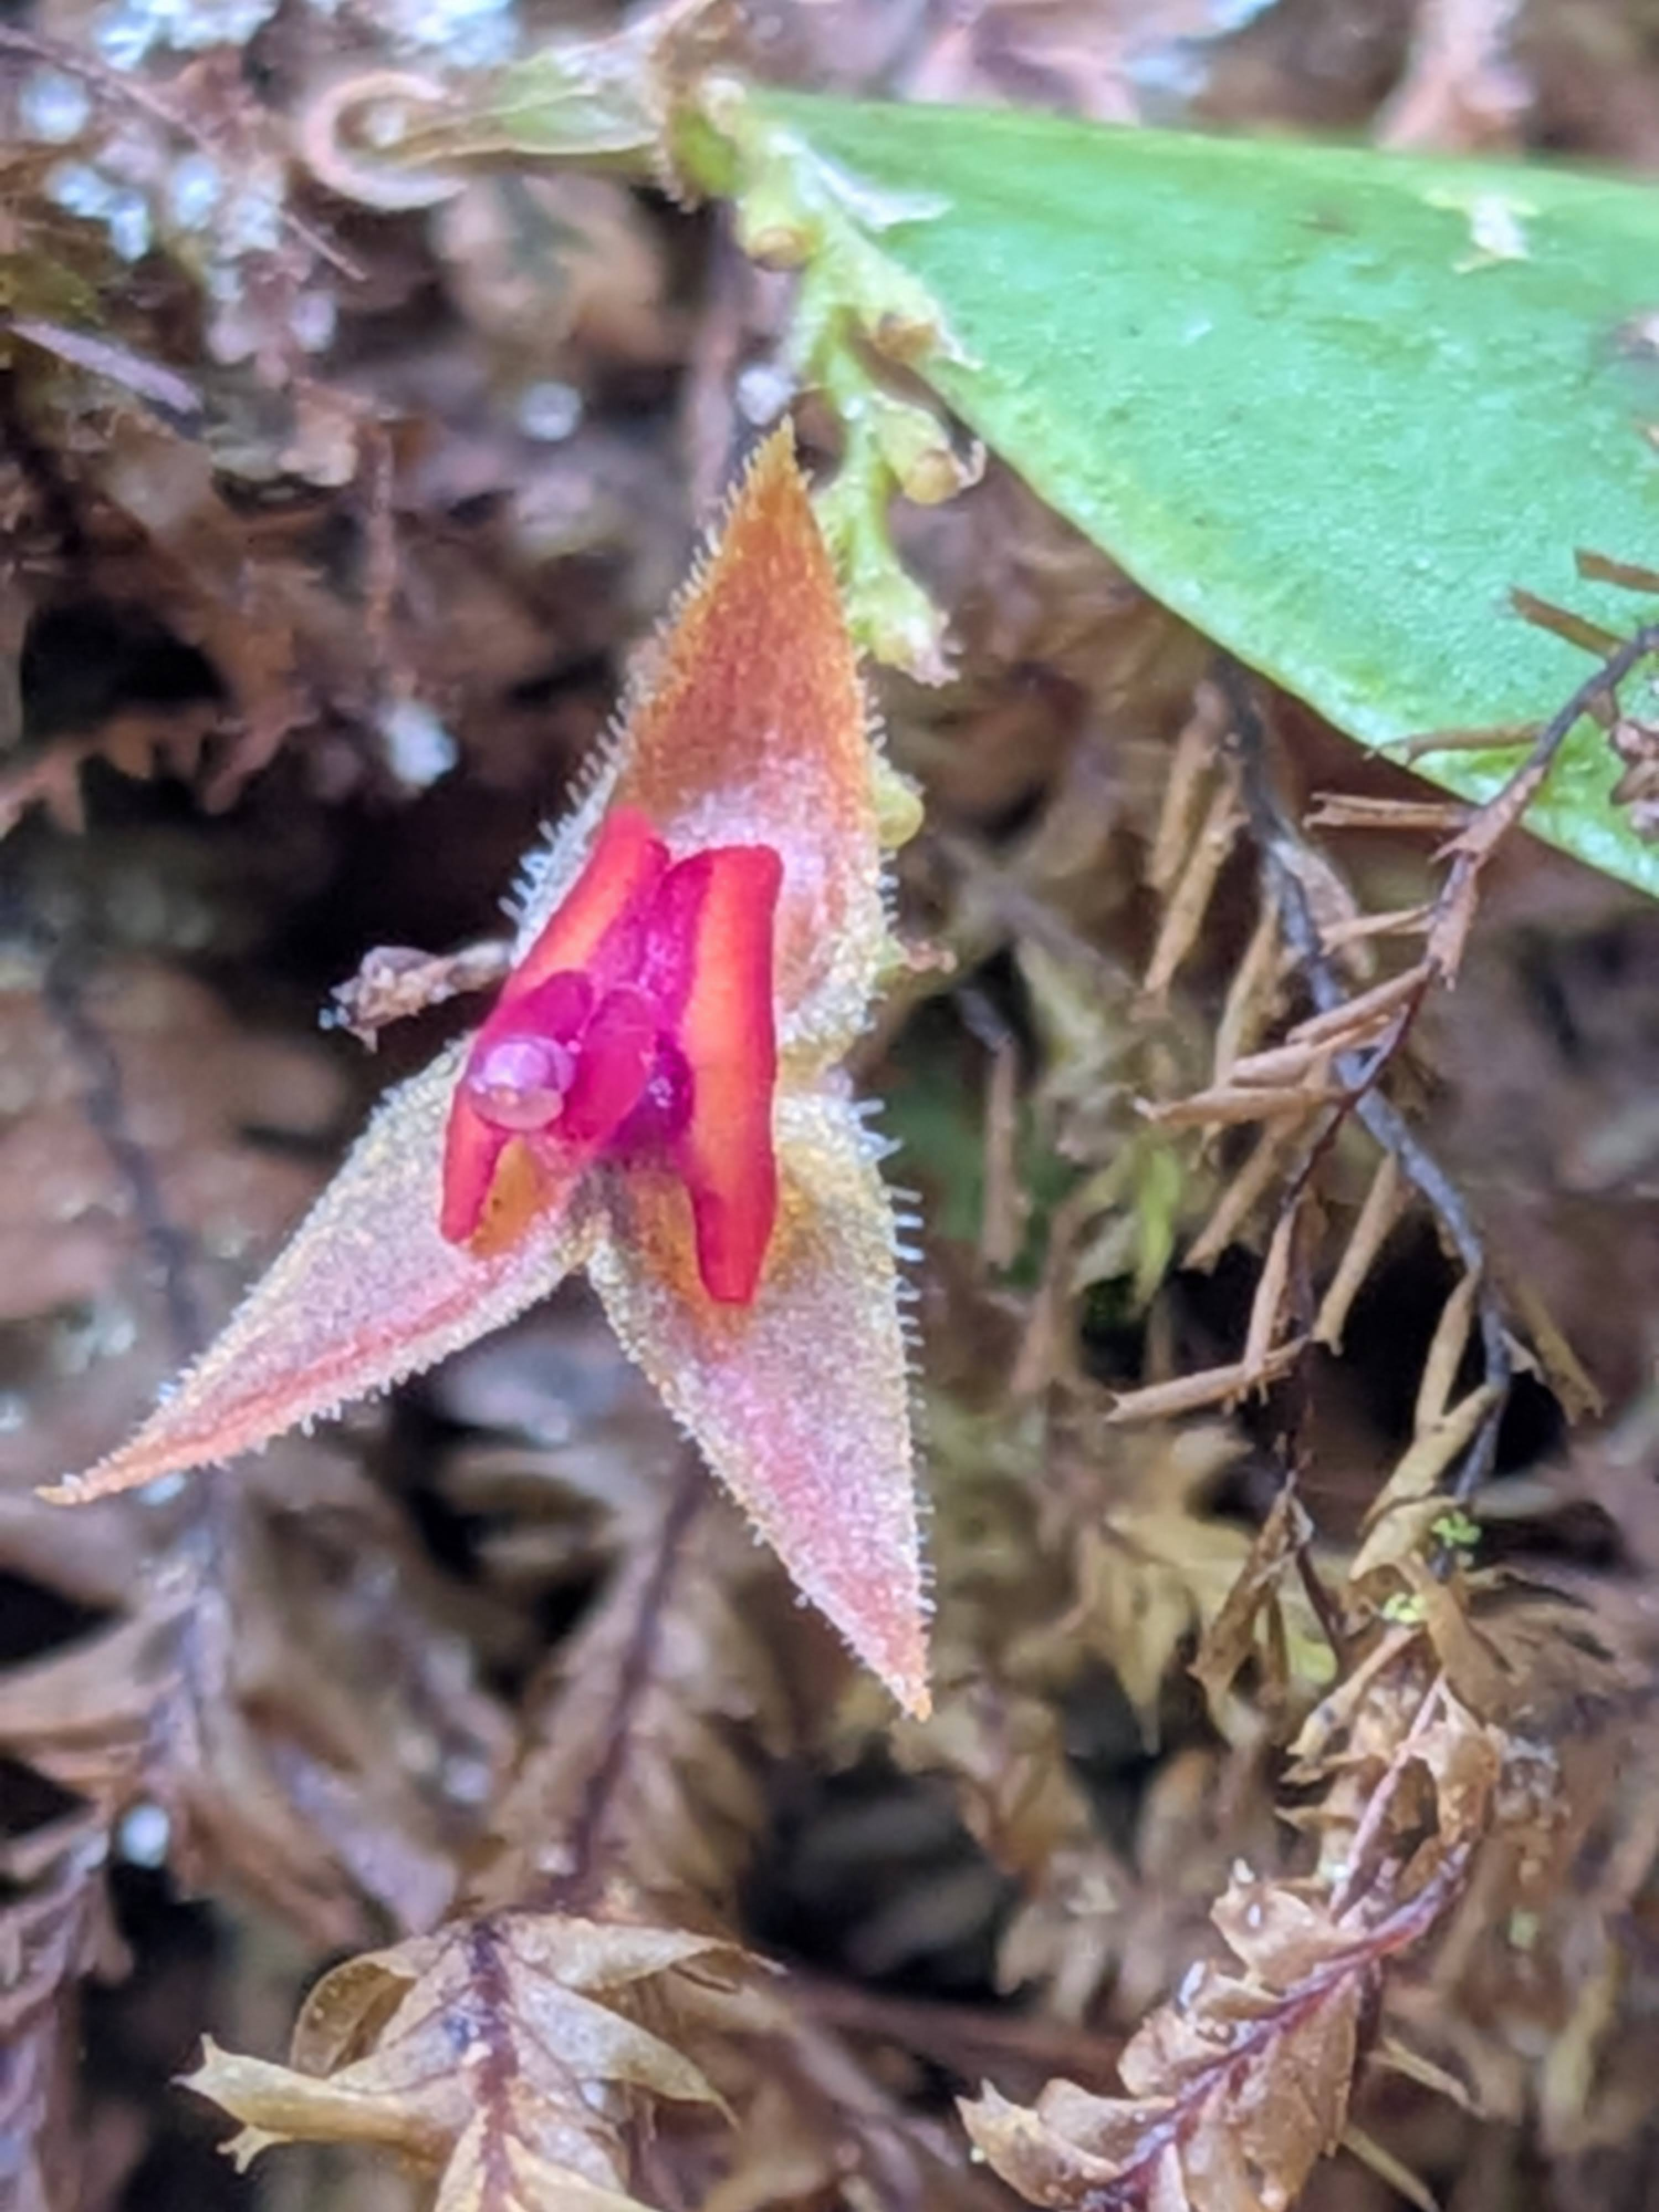
\includegraphics[keepaspectratio]{images/Lepanthes_eltoroensis_Edwin_Guevara.jpg}}

}

\caption{\emph{Lepanthes eltoroensis}. Foto: Edwin Guevara}

\end{figure}%

\begin{figure}[H]

{\centering \pandocbounded{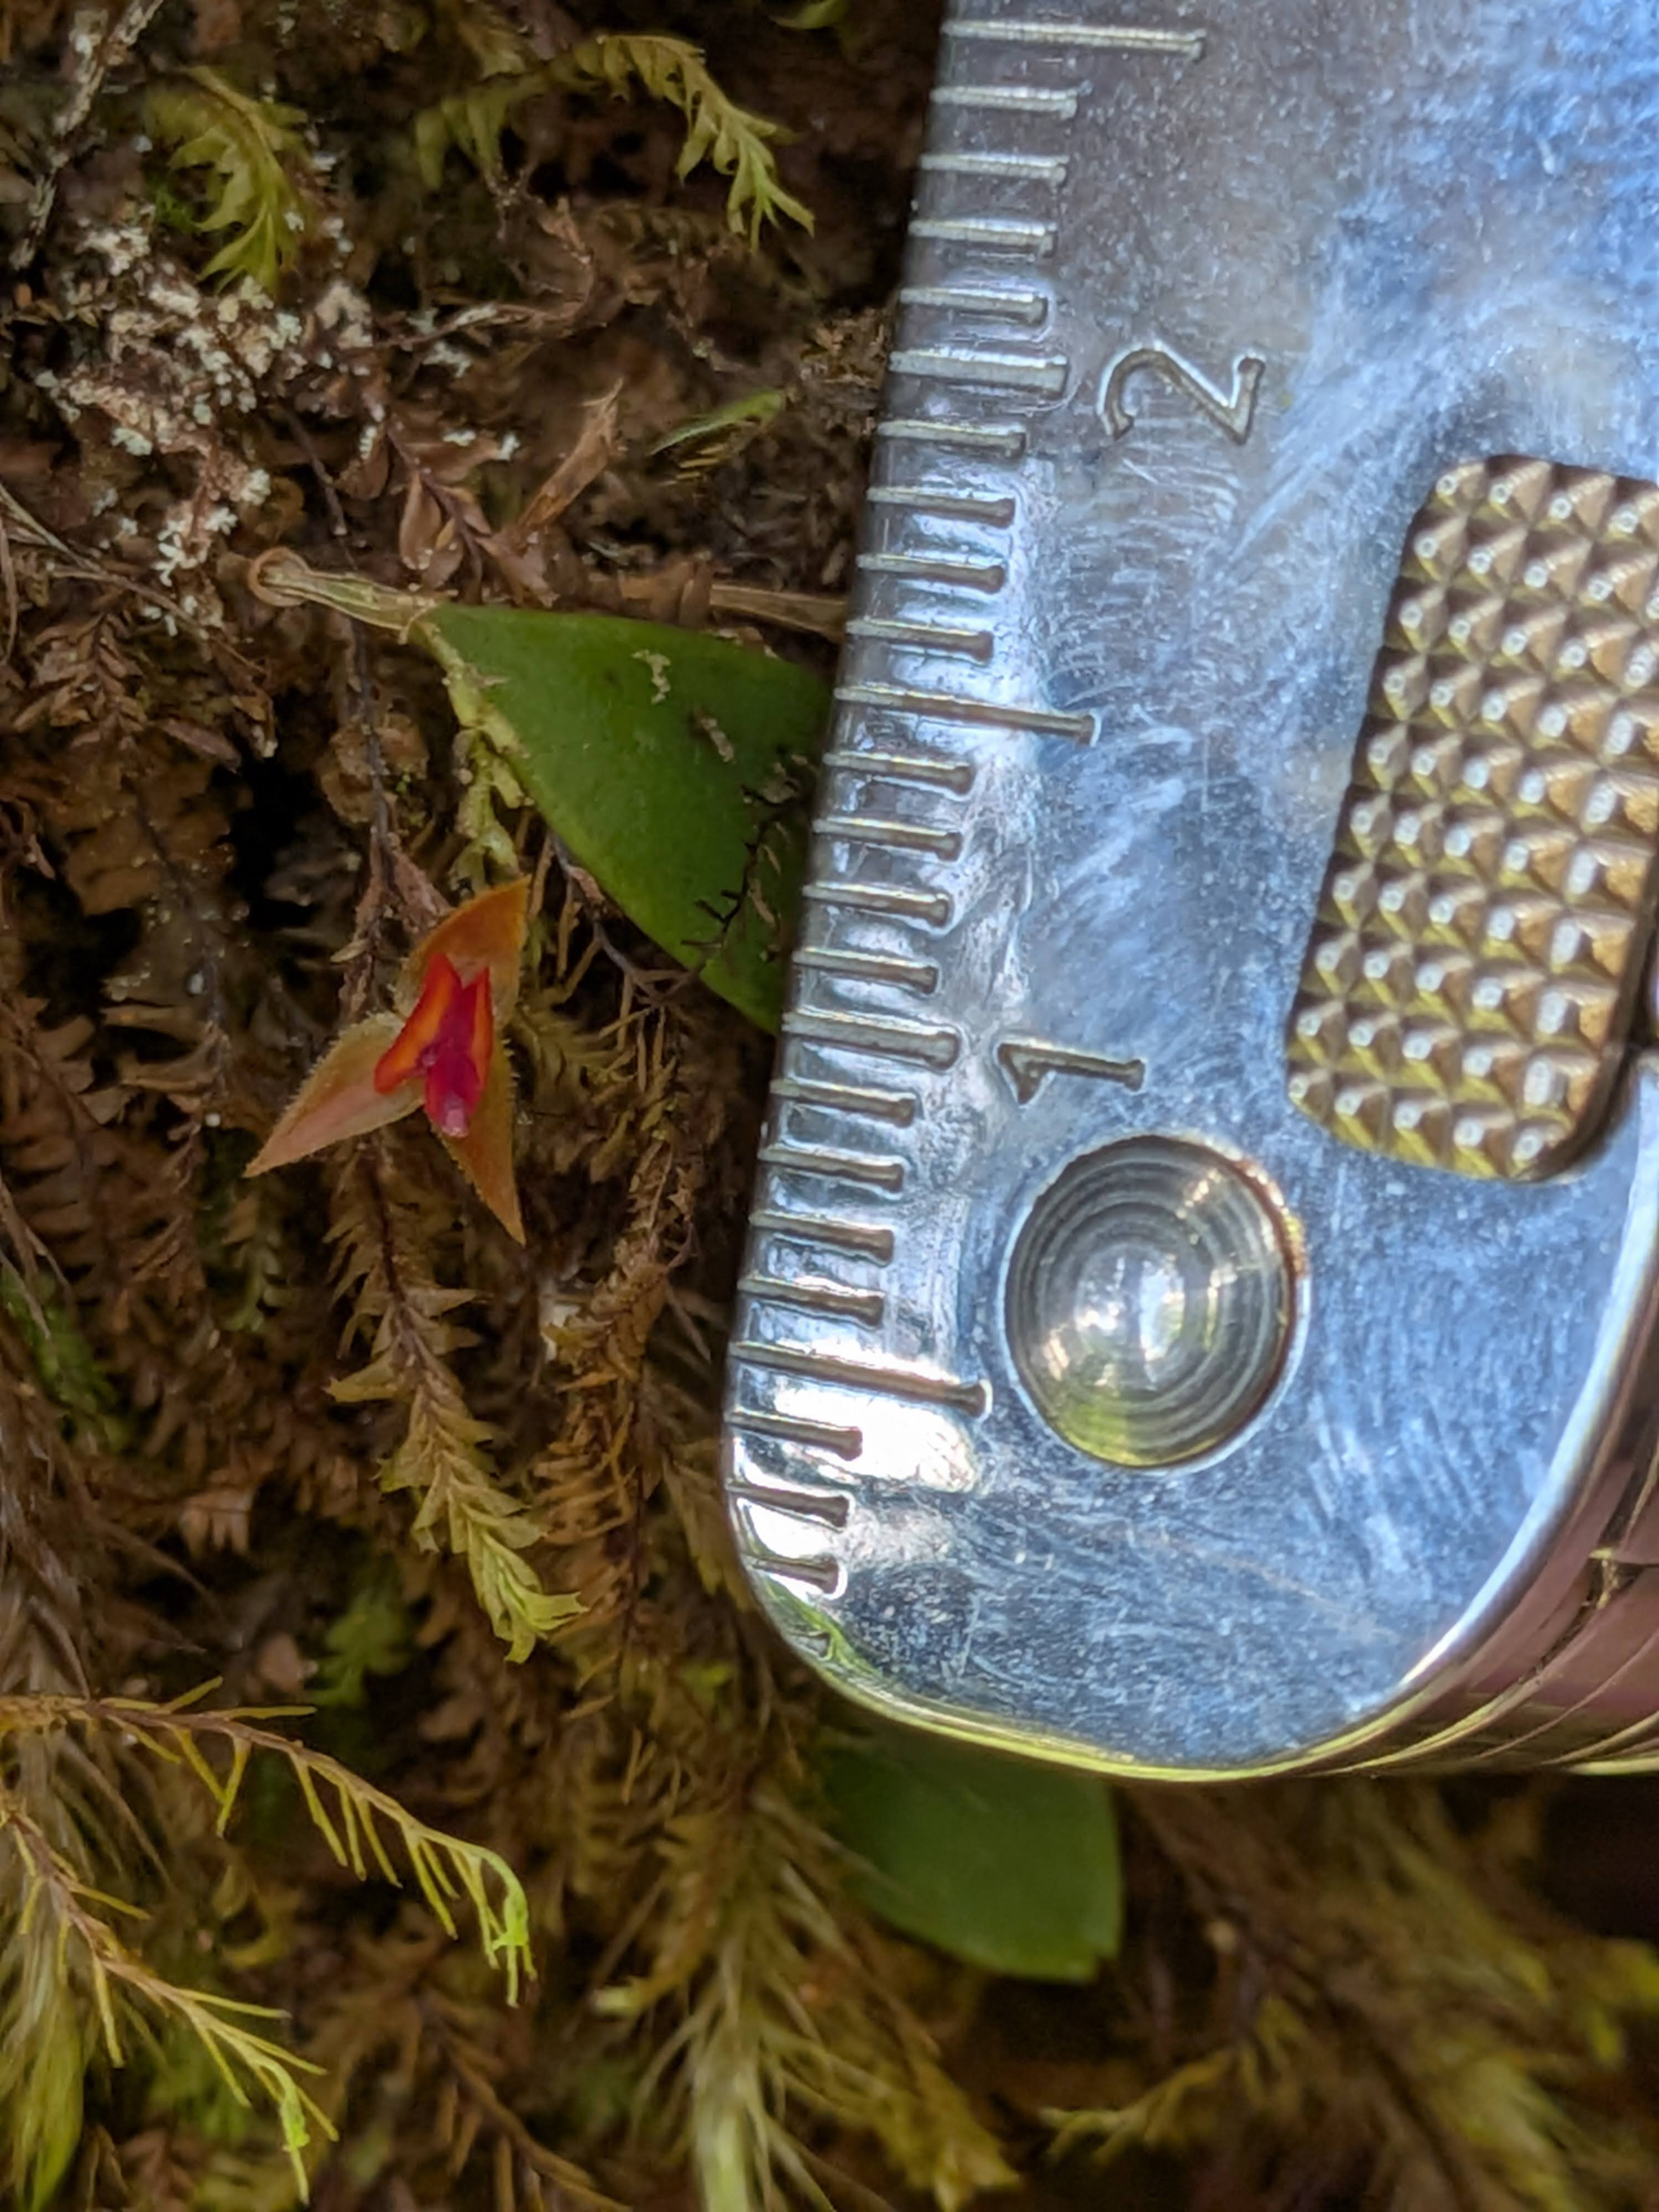
\includegraphics[keepaspectratio]{images/Lepanthes_eltoroensis_Phorophyte_Edwin_Guevara.jpg}}

}

\caption{\emph{Lepanthes eltoroensis}. Foto: Edwin Guevara}

\end{figure}%

\begin{center}\rule{0.5\linewidth}{0.5pt}\end{center}

\section{\texorpdfstring{Descargar los datos de una población de
\emph{L. eltoroensis} del paquete
\texttt{raretrans}}{Descargar los datos de una población de L. eltoroensis del paquete raretrans}}\label{descargar-los-datos-de-una-poblaciuxf3n-de-l.-eltoroensis-del-paquete-raretrans}

\begin{Shaded}
\begin{Highlighting}[]
\FunctionTok{data}\NormalTok{(}\StringTok{"L\_elto"}\NormalTok{) }\CommentTok{\# carga el conjunto de datos \textasciigrave{}L\_elto\textasciigrave{} en la memoria de la computadora (los datos están incluido en el paquete \textasciigrave{}raretrans\textasciigrave{})}
\FunctionTok{head}\NormalTok{(L\_elto) }\SpecialCharTok{|\textgreater{}} \FunctionTok{flextable}\NormalTok{()}
\end{Highlighting}
\end{Shaded}

\global\setlength{\Oldarrayrulewidth}{\arrayrulewidth}

\global\setlength{\Oldtabcolsep}{\tabcolsep}

\setlength{\tabcolsep}{2pt}

\renewcommand*{\arraystretch}{1.5}



\providecommand{\ascline}[3]{\noalign{\global\arrayrulewidth #1}\arrayrulecolor[HTML]{#2}\cline{#3}}

\begin{longtable*}[c]{ccccccccccccc}



\ascline{1.5pt}{666666}{1-13}

\multicolumn{1}{>{}r}{\textcolor[HTML]{000000}{\fontsize{11}{11}\selectfont{POPNUM}}} & \multicolumn{1}{>{}r}{\textcolor[HTML]{000000}{\fontsize{11}{11}\selectfont{year}}} & \multicolumn{1}{>{}r}{\textcolor[HTML]{000000}{\fontsize{11}{11}\selectfont{seedlings}}} & \multicolumn{1}{>{}r}{\textcolor[HTML]{000000}{\fontsize{11}{11}\selectfont{adults}}} & \multicolumn{1}{>{}r}{\textcolor[HTML]{000000}{\fontsize{11}{11}\selectfont{fertility}}} & \multicolumn{1}{>{}r}{\textcolor[HTML]{000000}{\fontsize{11}{11}\selectfont{IND\_NUM}}} & \multicolumn{1}{>{}l}{\textcolor[HTML]{000000}{\fontsize{11}{11}\selectfont{stage}}} & \multicolumn{1}{>{}l}{\textcolor[HTML]{000000}{\fontsize{11}{11}\selectfont{next\_stage}}} & \multicolumn{1}{>{}r}{\textcolor[HTML]{000000}{\fontsize{11}{11}\selectfont{first\_year}}} & \multicolumn{1}{>{}r}{\textcolor[HTML]{000000}{\fontsize{11}{11}\selectfont{last\_year}}} & \multicolumn{1}{>{}r}{\textcolor[HTML]{000000}{\fontsize{11}{11}\selectfont{recruited}}} & \multicolumn{1}{>{}r}{\textcolor[HTML]{000000}{\fontsize{11}{11}\selectfont{died}}} & \multicolumn{1}{>{}r}{\textcolor[HTML]{000000}{\fontsize{11}{11}\selectfont{lifespan}}} \\

\ascline{1.5pt}{666666}{1-13}\endfirsthead 

\ascline{1.5pt}{666666}{1-13}

\multicolumn{1}{>{}r}{\textcolor[HTML]{000000}{\fontsize{11}{11}\selectfont{POPNUM}}} & \multicolumn{1}{>{}r}{\textcolor[HTML]{000000}{\fontsize{11}{11}\selectfont{year}}} & \multicolumn{1}{>{}r}{\textcolor[HTML]{000000}{\fontsize{11}{11}\selectfont{seedlings}}} & \multicolumn{1}{>{}r}{\textcolor[HTML]{000000}{\fontsize{11}{11}\selectfont{adults}}} & \multicolumn{1}{>{}r}{\textcolor[HTML]{000000}{\fontsize{11}{11}\selectfont{fertility}}} & \multicolumn{1}{>{}r}{\textcolor[HTML]{000000}{\fontsize{11}{11}\selectfont{IND\_NUM}}} & \multicolumn{1}{>{}l}{\textcolor[HTML]{000000}{\fontsize{11}{11}\selectfont{stage}}} & \multicolumn{1}{>{}l}{\textcolor[HTML]{000000}{\fontsize{11}{11}\selectfont{next\_stage}}} & \multicolumn{1}{>{}r}{\textcolor[HTML]{000000}{\fontsize{11}{11}\selectfont{first\_year}}} & \multicolumn{1}{>{}r}{\textcolor[HTML]{000000}{\fontsize{11}{11}\selectfont{last\_year}}} & \multicolumn{1}{>{}r}{\textcolor[HTML]{000000}{\fontsize{11}{11}\selectfont{recruited}}} & \multicolumn{1}{>{}r}{\textcolor[HTML]{000000}{\fontsize{11}{11}\selectfont{died}}} & \multicolumn{1}{>{}r}{\textcolor[HTML]{000000}{\fontsize{11}{11}\selectfont{lifespan}}} \\

\ascline{1.5pt}{666666}{1-13}\endhead



\multicolumn{1}{>{}r}{\textcolor[HTML]{000000}{\fontsize{11}{11}\selectfont{209}}} & \multicolumn{1}{>{}r}{\textcolor[HTML]{000000}{\fontsize{11}{11}\selectfont{1}}} & \multicolumn{1}{>{}r}{\textcolor[HTML]{000000}{\fontsize{11}{11}\selectfont{1}}} & \multicolumn{1}{>{}r}{\textcolor[HTML]{000000}{\fontsize{11}{11}\selectfont{6}}} & \multicolumn{1}{>{}r}{\textcolor[HTML]{000000}{\fontsize{11}{11}\selectfont{0}}} & \multicolumn{1}{>{}r}{\textcolor[HTML]{000000}{\fontsize{11}{11}\selectfont{67}}} & \multicolumn{1}{>{}l}{\textcolor[HTML]{000000}{\fontsize{11}{11}\selectfont{j}}} & \multicolumn{1}{>{}l}{\textcolor[HTML]{000000}{\fontsize{11}{11}\selectfont{j}}} & \multicolumn{1}{>{}r}{\textcolor[HTML]{000000}{\fontsize{11}{11}\selectfont{1}}} & \multicolumn{1}{>{}r}{\textcolor[HTML]{000000}{\fontsize{11}{11}\selectfont{4}}} & \multicolumn{1}{>{}r}{\textcolor[HTML]{000000}{\fontsize{11}{11}\selectfont{true}}} & \multicolumn{1}{>{}r}{\textcolor[HTML]{000000}{\fontsize{11}{11}\selectfont{}}} & \multicolumn{1}{>{}r}{\textcolor[HTML]{000000}{\fontsize{11}{11}\selectfont{4}}} \\





\multicolumn{1}{>{}r}{\textcolor[HTML]{000000}{\fontsize{11}{11}\selectfont{209}}} & \multicolumn{1}{>{}r}{\textcolor[HTML]{000000}{\fontsize{11}{11}\selectfont{1}}} & \multicolumn{1}{>{}r}{\textcolor[HTML]{000000}{\fontsize{11}{11}\selectfont{1}}} & \multicolumn{1}{>{}r}{\textcolor[HTML]{000000}{\fontsize{11}{11}\selectfont{6}}} & \multicolumn{1}{>{}r}{\textcolor[HTML]{000000}{\fontsize{11}{11}\selectfont{0}}} & \multicolumn{1}{>{}r}{\textcolor[HTML]{000000}{\fontsize{11}{11}\selectfont{68}}} & \multicolumn{1}{>{}l}{\textcolor[HTML]{000000}{\fontsize{11}{11}\selectfont{a}}} & \multicolumn{1}{>{}l}{\textcolor[HTML]{000000}{\fontsize{11}{11}\selectfont{a}}} & \multicolumn{1}{>{}r}{\textcolor[HTML]{000000}{\fontsize{11}{11}\selectfont{1}}} & \multicolumn{1}{>{}r}{\textcolor[HTML]{000000}{\fontsize{11}{11}\selectfont{11}}} & \multicolumn{1}{>{}r}{\textcolor[HTML]{000000}{\fontsize{11}{11}\selectfont{true}}} & \multicolumn{1}{>{}r}{\textcolor[HTML]{000000}{\fontsize{11}{11}\selectfont{}}} & \multicolumn{1}{>{}r}{\textcolor[HTML]{000000}{\fontsize{11}{11}\selectfont{11}}} \\





\multicolumn{1}{>{}r}{\textcolor[HTML]{000000}{\fontsize{11}{11}\selectfont{209}}} & \multicolumn{1}{>{}r}{\textcolor[HTML]{000000}{\fontsize{11}{11}\selectfont{1}}} & \multicolumn{1}{>{}r}{\textcolor[HTML]{000000}{\fontsize{11}{11}\selectfont{1}}} & \multicolumn{1}{>{}r}{\textcolor[HTML]{000000}{\fontsize{11}{11}\selectfont{6}}} & \multicolumn{1}{>{}r}{\textcolor[HTML]{000000}{\fontsize{11}{11}\selectfont{0}}} & \multicolumn{1}{>{}r}{\textcolor[HTML]{000000}{\fontsize{11}{11}\selectfont{69}}} & \multicolumn{1}{>{}l}{\textcolor[HTML]{000000}{\fontsize{11}{11}\selectfont{a}}} & \multicolumn{1}{>{}l}{\textcolor[HTML]{000000}{\fontsize{11}{11}\selectfont{a}}} & \multicolumn{1}{>{}r}{\textcolor[HTML]{000000}{\fontsize{11}{11}\selectfont{1}}} & \multicolumn{1}{>{}r}{\textcolor[HTML]{000000}{\fontsize{11}{11}\selectfont{12}}} & \multicolumn{1}{>{}r}{\textcolor[HTML]{000000}{\fontsize{11}{11}\selectfont{true}}} & \multicolumn{1}{>{}r}{\textcolor[HTML]{000000}{\fontsize{11}{11}\selectfont{}}} & \multicolumn{1}{>{}r}{\textcolor[HTML]{000000}{\fontsize{11}{11}\selectfont{12}}} \\





\multicolumn{1}{>{}r}{\textcolor[HTML]{000000}{\fontsize{11}{11}\selectfont{209}}} & \multicolumn{1}{>{}r}{\textcolor[HTML]{000000}{\fontsize{11}{11}\selectfont{1}}} & \multicolumn{1}{>{}r}{\textcolor[HTML]{000000}{\fontsize{11}{11}\selectfont{1}}} & \multicolumn{1}{>{}r}{\textcolor[HTML]{000000}{\fontsize{11}{11}\selectfont{6}}} & \multicolumn{1}{>{}r}{\textcolor[HTML]{000000}{\fontsize{11}{11}\selectfont{0}}} & \multicolumn{1}{>{}r}{\textcolor[HTML]{000000}{\fontsize{11}{11}\selectfont{70}}} & \multicolumn{1}{>{}l}{\textcolor[HTML]{000000}{\fontsize{11}{11}\selectfont{a}}} & \multicolumn{1}{>{}l}{\textcolor[HTML]{000000}{\fontsize{11}{11}\selectfont{a}}} & \multicolumn{1}{>{}r}{\textcolor[HTML]{000000}{\fontsize{11}{11}\selectfont{1}}} & \multicolumn{1}{>{}r}{\textcolor[HTML]{000000}{\fontsize{11}{11}\selectfont{12}}} & \multicolumn{1}{>{}r}{\textcolor[HTML]{000000}{\fontsize{11}{11}\selectfont{true}}} & \multicolumn{1}{>{}r}{\textcolor[HTML]{000000}{\fontsize{11}{11}\selectfont{}}} & \multicolumn{1}{>{}r}{\textcolor[HTML]{000000}{\fontsize{11}{11}\selectfont{12}}} \\





\multicolumn{1}{>{}r}{\textcolor[HTML]{000000}{\fontsize{11}{11}\selectfont{209}}} & \multicolumn{1}{>{}r}{\textcolor[HTML]{000000}{\fontsize{11}{11}\selectfont{1}}} & \multicolumn{1}{>{}r}{\textcolor[HTML]{000000}{\fontsize{11}{11}\selectfont{1}}} & \multicolumn{1}{>{}r}{\textcolor[HTML]{000000}{\fontsize{11}{11}\selectfont{6}}} & \multicolumn{1}{>{}r}{\textcolor[HTML]{000000}{\fontsize{11}{11}\selectfont{0}}} & \multicolumn{1}{>{}r}{\textcolor[HTML]{000000}{\fontsize{11}{11}\selectfont{71}}} & \multicolumn{1}{>{}l}{\textcolor[HTML]{000000}{\fontsize{11}{11}\selectfont{j}}} & \multicolumn{1}{>{}l}{\textcolor[HTML]{000000}{\fontsize{11}{11}\selectfont{a}}} & \multicolumn{1}{>{}r}{\textcolor[HTML]{000000}{\fontsize{11}{11}\selectfont{1}}} & \multicolumn{1}{>{}r}{\textcolor[HTML]{000000}{\fontsize{11}{11}\selectfont{12}}} & \multicolumn{1}{>{}r}{\textcolor[HTML]{000000}{\fontsize{11}{11}\selectfont{true}}} & \multicolumn{1}{>{}r}{\textcolor[HTML]{000000}{\fontsize{11}{11}\selectfont{}}} & \multicolumn{1}{>{}r}{\textcolor[HTML]{000000}{\fontsize{11}{11}\selectfont{12}}} \\





\multicolumn{1}{>{}r}{\textcolor[HTML]{000000}{\fontsize{11}{11}\selectfont{209}}} & \multicolumn{1}{>{}r}{\textcolor[HTML]{000000}{\fontsize{11}{11}\selectfont{1}}} & \multicolumn{1}{>{}r}{\textcolor[HTML]{000000}{\fontsize{11}{11}\selectfont{1}}} & \multicolumn{1}{>{}r}{\textcolor[HTML]{000000}{\fontsize{11}{11}\selectfont{6}}} & \multicolumn{1}{>{}r}{\textcolor[HTML]{000000}{\fontsize{11}{11}\selectfont{0}}} & \multicolumn{1}{>{}r}{\textcolor[HTML]{000000}{\fontsize{11}{11}\selectfont{72}}} & \multicolumn{1}{>{}l}{\textcolor[HTML]{000000}{\fontsize{11}{11}\selectfont{a}}} & \multicolumn{1}{>{}l}{\textcolor[HTML]{000000}{\fontsize{11}{11}\selectfont{a}}} & \multicolumn{1}{>{}r}{\textcolor[HTML]{000000}{\fontsize{11}{11}\selectfont{1}}} & \multicolumn{1}{>{}r}{\textcolor[HTML]{000000}{\fontsize{11}{11}\selectfont{5}}} & \multicolumn{1}{>{}r}{\textcolor[HTML]{000000}{\fontsize{11}{11}\selectfont{true}}} & \multicolumn{1}{>{}r}{\textcolor[HTML]{000000}{\fontsize{11}{11}\selectfont{}}} & \multicolumn{1}{>{}r}{\textcolor[HTML]{000000}{\fontsize{11}{11}\selectfont{5}}} \\

\ascline{1.5pt}{666666}{1-13}



\end{longtable*}



\arrayrulecolor[HTML]{000000}

\global\setlength{\arrayrulewidth}{\Oldarrayrulewidth}

\global\setlength{\tabcolsep}{\Oldtabcolsep}

\renewcommand*{\arraystretch}{1}

\section{Organización de los datos en el
``data.frame''}\label{organizaciuxf3n-de-los-datos-en-el-data.frame}

Supongamos que tienes una base de datos llamada \texttt{L\_elto} con las
siguientes columnas:

\begin{itemize}
\tightlist
\item
  \texttt{pop}: identificador de la población
\item
  \texttt{period}: periodo de tiempo
\item
  \texttt{stage}: etapa actual del individuo
\item
  \texttt{next\_stage}: etapa siguiente
\item
  \texttt{fertility}: indicador de fecundidad
\end{itemize}

Seleccionamos la población POPNUM 250 y el periodo 5:

El primer paso es seleccionar los datos de la población y el periodo de
tiempo que queremos analizar. Posteriormente, cambiamos el nombre del
estado más pequeño a ``seedling''. Este paso no es estrictamente
necesario pero nos ayuda a entender más fácilmente la nomenclatura.

La base de datos \texttt{L\_elto} está compuesta por datos individuales
del estado actual (\texttt{stage}, periodo \textbf{t}), del estado
siguiente (\texttt{next\_stage}, periodo \textbf{t+1}) y de la
fertilidad. Tenga en cuenta que aquí ``p'' significa ``plántula'' por la
traducción al español. En la siguiente caja de código las primeras
líneas seleccionan la población de interés y el periodo de tiempo sobre
el que queremos trabajar y cambian el nombre de la etapa del ciclo vital
de ``p'' a ``s''.

\begin{Shaded}
\begin{Highlighting}[]
\NormalTok{onepop }\OtherTok{\textless{}{-}}\NormalTok{ L\_elto }\SpecialCharTok{\%\textgreater{}\%}

  \FunctionTok{filter}\NormalTok{(POPNUM }\SpecialCharTok{==} \DecValTok{250}\NormalTok{, year }\SpecialCharTok{==} \DecValTok{5}\NormalTok{) }\SpecialCharTok{\%\textgreater{}\%} \CommentTok{\# Filtrar la población \# 250, el periodo (año=year) 5}

  \FunctionTok{mutate}\NormalTok{(}
    \AttributeTok{stage =} \FunctionTok{case\_when}\NormalTok{(stage }\SpecialCharTok{==} \StringTok{"p"} \SpecialCharTok{\textasciitilde{}} \StringTok{"s"}\NormalTok{, }\ConstantTok{TRUE} \SpecialCharTok{\textasciitilde{}}\NormalTok{ stage),}
    \AttributeTok{next\_stage =} \FunctionTok{case\_when}\NormalTok{(next\_stage }\SpecialCharTok{==} \StringTok{"p"} \SpecialCharTok{\textasciitilde{}} \StringTok{"s"}\NormalTok{, }\ConstantTok{TRUE} \SpecialCharTok{\textasciitilde{}}\NormalTok{ next\_stage)}
\NormalTok{  ) }\CommentTok{\# redefine "p" por plantula a "s" para seedling}
\end{Highlighting}
\end{Shaded}

En el siguiente código usamos la función
\texttt{popbio::projection.matrix()} para crear la matriz de proyección
poblacional. Tenemos ahora nuestra matriz de transición y fecundidad
basadas en los datos de la población \#250 del periodo 5. La función
\texttt{projection.matrix()} requiere que se especifiquen los nombres de
las etapas y los estados siguientes, así como el nombre de la columna de
fecundidad. En este caso, las etapas son ``s'' (plántula), ``j''
(juvenil) y ``a'' (adulto), y el estado siguiente es
\texttt{next\_stage}. La columna de fecundidad se llama
\texttt{fertility}. El argumento \texttt{sort} especifica el orden en
que queremos que aparezcan las etapas en la matriz.

Solamente los adultos pueden producir plántulas, por lo que la matriz de
fecundidad tiene un valor solamente en la posición (1,3), (plántula,
adulto). La función \texttt{projection.matrix()} devuelve una lista con
dos matrices: una de transición y otra de fecundidad. La matriz de
transición es una matriz cuadrada que muestra las probabilidades de
transición entre las etapas, mientras que la matriz de fecundidad es una
matriz que muestra la fecundidad por etapa.

A partir de este punto los análisis se llevan a cabo considerando
\textbf{s} (plántula), \textbf{j} (juvenil) y \textbf{a} (adulto), y las
dos matrices: \textbf{T} (transición de estadios) y \textbf{F}
(fecundidad). La tasa de crecimiento asintótica de la población
observada es \(\lambda\). Las transiciones raras que faltan en nuestra
primera matriz de transición \texttt{TF\$T}, pero que sabemos que
ocurren, son la transición de plántula (\emph{s}) a adulto (\emph{a}) y
la transición de \emph{j} a \emph{s}.

\begin{Shaded}
\begin{Highlighting}[]
\CommentTok{\# popbio::projection.matrix no funciona con el formato *tibbles*, por consecuencia se convierte en data.frame}

\FunctionTok{head}\NormalTok{(onepop) }\SpecialCharTok{|\textgreater{}} \FunctionTok{flextable}\NormalTok{() }\CommentTok{\# Ahora tenemos solamente datos de la población \#250 del periodo 5}
\end{Highlighting}
\end{Shaded}

\global\setlength{\Oldarrayrulewidth}{\arrayrulewidth}

\global\setlength{\Oldtabcolsep}{\tabcolsep}

\setlength{\tabcolsep}{2pt}

\renewcommand*{\arraystretch}{1.5}



\providecommand{\ascline}[3]{\noalign{\global\arrayrulewidth #1}\arrayrulecolor[HTML]{#2}\cline{#3}}

\begin{longtable*}[c]{ccccccccccccc}



\ascline{1.5pt}{666666}{1-13}

\multicolumn{1}{>{}r}{\textcolor[HTML]{000000}{\fontsize{11}{11}\selectfont{POPNUM}}} & \multicolumn{1}{>{}r}{\textcolor[HTML]{000000}{\fontsize{11}{11}\selectfont{year}}} & \multicolumn{1}{>{}r}{\textcolor[HTML]{000000}{\fontsize{11}{11}\selectfont{seedlings}}} & \multicolumn{1}{>{}r}{\textcolor[HTML]{000000}{\fontsize{11}{11}\selectfont{adults}}} & \multicolumn{1}{>{}r}{\textcolor[HTML]{000000}{\fontsize{11}{11}\selectfont{fertility}}} & \multicolumn{1}{>{}r}{\textcolor[HTML]{000000}{\fontsize{11}{11}\selectfont{IND\_NUM}}} & \multicolumn{1}{>{}l}{\textcolor[HTML]{000000}{\fontsize{11}{11}\selectfont{stage}}} & \multicolumn{1}{>{}l}{\textcolor[HTML]{000000}{\fontsize{11}{11}\selectfont{next\_stage}}} & \multicolumn{1}{>{}r}{\textcolor[HTML]{000000}{\fontsize{11}{11}\selectfont{first\_year}}} & \multicolumn{1}{>{}r}{\textcolor[HTML]{000000}{\fontsize{11}{11}\selectfont{last\_year}}} & \multicolumn{1}{>{}r}{\textcolor[HTML]{000000}{\fontsize{11}{11}\selectfont{recruited}}} & \multicolumn{1}{>{}r}{\textcolor[HTML]{000000}{\fontsize{11}{11}\selectfont{died}}} & \multicolumn{1}{>{}r}{\textcolor[HTML]{000000}{\fontsize{11}{11}\selectfont{lifespan}}} \\

\ascline{1.5pt}{666666}{1-13}\endfirsthead 

\ascline{1.5pt}{666666}{1-13}

\multicolumn{1}{>{}r}{\textcolor[HTML]{000000}{\fontsize{11}{11}\selectfont{POPNUM}}} & \multicolumn{1}{>{}r}{\textcolor[HTML]{000000}{\fontsize{11}{11}\selectfont{year}}} & \multicolumn{1}{>{}r}{\textcolor[HTML]{000000}{\fontsize{11}{11}\selectfont{seedlings}}} & \multicolumn{1}{>{}r}{\textcolor[HTML]{000000}{\fontsize{11}{11}\selectfont{adults}}} & \multicolumn{1}{>{}r}{\textcolor[HTML]{000000}{\fontsize{11}{11}\selectfont{fertility}}} & \multicolumn{1}{>{}r}{\textcolor[HTML]{000000}{\fontsize{11}{11}\selectfont{IND\_NUM}}} & \multicolumn{1}{>{}l}{\textcolor[HTML]{000000}{\fontsize{11}{11}\selectfont{stage}}} & \multicolumn{1}{>{}l}{\textcolor[HTML]{000000}{\fontsize{11}{11}\selectfont{next\_stage}}} & \multicolumn{1}{>{}r}{\textcolor[HTML]{000000}{\fontsize{11}{11}\selectfont{first\_year}}} & \multicolumn{1}{>{}r}{\textcolor[HTML]{000000}{\fontsize{11}{11}\selectfont{last\_year}}} & \multicolumn{1}{>{}r}{\textcolor[HTML]{000000}{\fontsize{11}{11}\selectfont{recruited}}} & \multicolumn{1}{>{}r}{\textcolor[HTML]{000000}{\fontsize{11}{11}\selectfont{died}}} & \multicolumn{1}{>{}r}{\textcolor[HTML]{000000}{\fontsize{11}{11}\selectfont{lifespan}}} \\

\ascline{1.5pt}{666666}{1-13}\endhead



\multicolumn{1}{>{}r}{\textcolor[HTML]{000000}{\fontsize{11}{11}\selectfont{250}}} & \multicolumn{1}{>{}r}{\textcolor[HTML]{000000}{\fontsize{11}{11}\selectfont{5}}} & \multicolumn{1}{>{}r}{\textcolor[HTML]{000000}{\fontsize{11}{11}\selectfont{8}}} & \multicolumn{1}{>{}r}{\textcolor[HTML]{000000}{\fontsize{11}{11}\selectfont{34}}} & \multicolumn{1}{>{}r}{\textcolor[HTML]{000000}{\fontsize{11}{11}\selectfont{0.0000000}}} & \multicolumn{1}{>{}r}{\textcolor[HTML]{000000}{\fontsize{11}{11}\selectfont{167}}} & \multicolumn{1}{>{}l}{\textcolor[HTML]{000000}{\fontsize{11}{11}\selectfont{j}}} & \multicolumn{1}{>{}l}{\textcolor[HTML]{000000}{\fontsize{11}{11}\selectfont{a}}} & \multicolumn{1}{>{}r}{\textcolor[HTML]{000000}{\fontsize{11}{11}\selectfont{1}}} & \multicolumn{1}{>{}r}{\textcolor[HTML]{000000}{\fontsize{11}{11}\selectfont{9}}} & \multicolumn{1}{>{}r}{\textcolor[HTML]{000000}{\fontsize{11}{11}\selectfont{false}}} & \multicolumn{1}{>{}r}{\textcolor[HTML]{000000}{\fontsize{11}{11}\selectfont{}}} & \multicolumn{1}{>{}r}{\textcolor[HTML]{000000}{\fontsize{11}{11}\selectfont{9}}} \\





\multicolumn{1}{>{}r}{\textcolor[HTML]{000000}{\fontsize{11}{11}\selectfont{250}}} & \multicolumn{1}{>{}r}{\textcolor[HTML]{000000}{\fontsize{11}{11}\selectfont{5}}} & \multicolumn{1}{>{}r}{\textcolor[HTML]{000000}{\fontsize{11}{11}\selectfont{8}}} & \multicolumn{1}{>{}r}{\textcolor[HTML]{000000}{\fontsize{11}{11}\selectfont{34}}} & \multicolumn{1}{>{}r}{\textcolor[HTML]{000000}{\fontsize{11}{11}\selectfont{0.0000000}}} & \multicolumn{1}{>{}r}{\textcolor[HTML]{000000}{\fontsize{11}{11}\selectfont{168}}} & \multicolumn{1}{>{}l}{\textcolor[HTML]{000000}{\fontsize{11}{11}\selectfont{j}}} & \multicolumn{1}{>{}l}{\textcolor[HTML]{000000}{\fontsize{11}{11}\selectfont{a}}} & \multicolumn{1}{>{}r}{\textcolor[HTML]{000000}{\fontsize{11}{11}\selectfont{1}}} & \multicolumn{1}{>{}r}{\textcolor[HTML]{000000}{\fontsize{11}{11}\selectfont{12}}} & \multicolumn{1}{>{}r}{\textcolor[HTML]{000000}{\fontsize{11}{11}\selectfont{false}}} & \multicolumn{1}{>{}r}{\textcolor[HTML]{000000}{\fontsize{11}{11}\selectfont{}}} & \multicolumn{1}{>{}r}{\textcolor[HTML]{000000}{\fontsize{11}{11}\selectfont{12}}} \\





\multicolumn{1}{>{}r}{\textcolor[HTML]{000000}{\fontsize{11}{11}\selectfont{250}}} & \multicolumn{1}{>{}r}{\textcolor[HTML]{000000}{\fontsize{11}{11}\selectfont{5}}} & \multicolumn{1}{>{}r}{\textcolor[HTML]{000000}{\fontsize{11}{11}\selectfont{8}}} & \multicolumn{1}{>{}r}{\textcolor[HTML]{000000}{\fontsize{11}{11}\selectfont{34}}} & \multicolumn{1}{>{}r}{\textcolor[HTML]{000000}{\fontsize{11}{11}\selectfont{0.0000000}}} & \multicolumn{1}{>{}r}{\textcolor[HTML]{000000}{\fontsize{11}{11}\selectfont{169}}} & \multicolumn{1}{>{}l}{\textcolor[HTML]{000000}{\fontsize{11}{11}\selectfont{j}}} & \multicolumn{1}{>{}l}{\textcolor[HTML]{000000}{\fontsize{11}{11}\selectfont{a}}} & \multicolumn{1}{>{}r}{\textcolor[HTML]{000000}{\fontsize{11}{11}\selectfont{1}}} & \multicolumn{1}{>{}r}{\textcolor[HTML]{000000}{\fontsize{11}{11}\selectfont{12}}} & \multicolumn{1}{>{}r}{\textcolor[HTML]{000000}{\fontsize{11}{11}\selectfont{false}}} & \multicolumn{1}{>{}r}{\textcolor[HTML]{000000}{\fontsize{11}{11}\selectfont{}}} & \multicolumn{1}{>{}r}{\textcolor[HTML]{000000}{\fontsize{11}{11}\selectfont{12}}} \\





\multicolumn{1}{>{}r}{\textcolor[HTML]{000000}{\fontsize{11}{11}\selectfont{250}}} & \multicolumn{1}{>{}r}{\textcolor[HTML]{000000}{\fontsize{11}{11}\selectfont{5}}} & \multicolumn{1}{>{}r}{\textcolor[HTML]{000000}{\fontsize{11}{11}\selectfont{8}}} & \multicolumn{1}{>{}r}{\textcolor[HTML]{000000}{\fontsize{11}{11}\selectfont{34}}} & \multicolumn{1}{>{}r}{\textcolor[HTML]{000000}{\fontsize{11}{11}\selectfont{0.1176471}}} & \multicolumn{1}{>{}r}{\textcolor[HTML]{000000}{\fontsize{11}{11}\selectfont{170}}} & \multicolumn{1}{>{}l}{\textcolor[HTML]{000000}{\fontsize{11}{11}\selectfont{a}}} & \multicolumn{1}{>{}l}{\textcolor[HTML]{000000}{\fontsize{11}{11}\selectfont{a}}} & \multicolumn{1}{>{}r}{\textcolor[HTML]{000000}{\fontsize{11}{11}\selectfont{1}}} & \multicolumn{1}{>{}r}{\textcolor[HTML]{000000}{\fontsize{11}{11}\selectfont{12}}} & \multicolumn{1}{>{}r}{\textcolor[HTML]{000000}{\fontsize{11}{11}\selectfont{false}}} & \multicolumn{1}{>{}r}{\textcolor[HTML]{000000}{\fontsize{11}{11}\selectfont{}}} & \multicolumn{1}{>{}r}{\textcolor[HTML]{000000}{\fontsize{11}{11}\selectfont{12}}} \\





\multicolumn{1}{>{}r}{\textcolor[HTML]{000000}{\fontsize{11}{11}\selectfont{250}}} & \multicolumn{1}{>{}r}{\textcolor[HTML]{000000}{\fontsize{11}{11}\selectfont{5}}} & \multicolumn{1}{>{}r}{\textcolor[HTML]{000000}{\fontsize{11}{11}\selectfont{8}}} & \multicolumn{1}{>{}r}{\textcolor[HTML]{000000}{\fontsize{11}{11}\selectfont{34}}} & \multicolumn{1}{>{}r}{\textcolor[HTML]{000000}{\fontsize{11}{11}\selectfont{0.0000000}}} & \multicolumn{1}{>{}r}{\textcolor[HTML]{000000}{\fontsize{11}{11}\selectfont{172}}} & \multicolumn{1}{>{}l}{\textcolor[HTML]{000000}{\fontsize{11}{11}\selectfont{j}}} & \multicolumn{1}{>{}l}{\textcolor[HTML]{000000}{\fontsize{11}{11}\selectfont{j}}} & \multicolumn{1}{>{}r}{\textcolor[HTML]{000000}{\fontsize{11}{11}\selectfont{1}}} & \multicolumn{1}{>{}r}{\textcolor[HTML]{000000}{\fontsize{11}{11}\selectfont{11}}} & \multicolumn{1}{>{}r}{\textcolor[HTML]{000000}{\fontsize{11}{11}\selectfont{false}}} & \multicolumn{1}{>{}r}{\textcolor[HTML]{000000}{\fontsize{11}{11}\selectfont{}}} & \multicolumn{1}{>{}r}{\textcolor[HTML]{000000}{\fontsize{11}{11}\selectfont{11}}} \\





\multicolumn{1}{>{}r}{\textcolor[HTML]{000000}{\fontsize{11}{11}\selectfont{250}}} & \multicolumn{1}{>{}r}{\textcolor[HTML]{000000}{\fontsize{11}{11}\selectfont{5}}} & \multicolumn{1}{>{}r}{\textcolor[HTML]{000000}{\fontsize{11}{11}\selectfont{8}}} & \multicolumn{1}{>{}r}{\textcolor[HTML]{000000}{\fontsize{11}{11}\selectfont{34}}} & \multicolumn{1}{>{}r}{\textcolor[HTML]{000000}{\fontsize{11}{11}\selectfont{0.0000000}}} & \multicolumn{1}{>{}r}{\textcolor[HTML]{000000}{\fontsize{11}{11}\selectfont{173}}} & \multicolumn{1}{>{}l}{\textcolor[HTML]{000000}{\fontsize{11}{11}\selectfont{j}}} & \multicolumn{1}{>{}l}{\textcolor[HTML]{000000}{\fontsize{11}{11}\selectfont{a}}} & \multicolumn{1}{>{}r}{\textcolor[HTML]{000000}{\fontsize{11}{11}\selectfont{1}}} & \multicolumn{1}{>{}r}{\textcolor[HTML]{000000}{\fontsize{11}{11}\selectfont{12}}} & \multicolumn{1}{>{}r}{\textcolor[HTML]{000000}{\fontsize{11}{11}\selectfont{false}}} & \multicolumn{1}{>{}r}{\textcolor[HTML]{000000}{\fontsize{11}{11}\selectfont{}}} & \multicolumn{1}{>{}r}{\textcolor[HTML]{000000}{\fontsize{11}{11}\selectfont{12}}} \\

\ascline{1.5pt}{666666}{1-13}



\end{longtable*}



\arrayrulecolor[HTML]{000000}

\global\setlength{\arrayrulewidth}{\Oldarrayrulewidth}

\global\setlength{\tabcolsep}{\Oldtabcolsep}

\renewcommand*{\arraystretch}{1}

\begin{Shaded}
\begin{Highlighting}[]
\CommentTok{\# Crear TF = TRUE, añadir para formatear correctamente.}
\NormalTok{TF }\OtherTok{\textless{}{-}}\NormalTok{ popbio}\SpecialCharTok{::}\FunctionTok{projection.matrix}\NormalTok{(}
  \FunctionTok{as.data.frame}\NormalTok{(onepop),}
  \AttributeTok{stage =}\NormalTok{ stage,}
  \AttributeTok{fate =}\NormalTok{ next\_stage,}
  \AttributeTok{fertility =} \StringTok{"fertility"}\NormalTok{,}
  \AttributeTok{sort =} \FunctionTok{c}\NormalTok{(}\StringTok{"s"}\NormalTok{, }\StringTok{"j"}\NormalTok{, }\StringTok{"a"}\NormalTok{),}
  \AttributeTok{TF =} \ConstantTok{TRUE}
\NormalTok{)}
\NormalTok{TF }\CommentTok{\# Esta es la estructura de etapas de vida para esa población. Nota que tenemos dos matrices, una de transiciones **T** y otra de fecundidad **F**.}
\end{Highlighting}
\end{Shaded}

\begin{verbatim}
$T
   
             s          j          a
  s 0.09090909 0.00000000 0.00000000
  j 0.63636364 0.57446809 0.00000000
  a 0.00000000 0.29787234 0.85294118

$F
   
            s         j         a
  s 0.0000000 0.0000000 0.1176471
  j 0.0000000 0.0000000 0.0000000
  a 0.0000000 0.0000000 0.0000000
\end{verbatim}

\begin{center}\rule{0.5\linewidth}{0.5pt}\end{center}

\section{Obtener el número inicial de individuos por
etapa}\label{obtener-el-nuxfamero-inicial-de-individuos-por-etapa}

Dado que nuestros conteos (número de individuos), \(N\), y el tamaño de
\emph{muestra equivalente} \emph{a priori} se expresan como múltiplos
del número de individuos observados, necesitamos obtener el número de
individuos en cada etapa (\(N\)) en el primer periodo de tiempo. Para
esto utilizamos la función \texttt{raretrans::get\_state\_vector()}. Se
observa que la cantidad de individuos iniciales por etapa ---es decir,
el número de individuos en el primer muestreo--- es muy limitada: 11
plántulas, 47 juveniles y 34 adultos para esta población en este periodo
de muestreo.

\begin{Shaded}
\begin{Highlighting}[]
\NormalTok{N }\OtherTok{\textless{}{-}} \FunctionTok{get\_state\_vector}\NormalTok{(onepop, }\AttributeTok{stage =}\NormalTok{ stage, }\AttributeTok{sort =} \FunctionTok{c}\NormalTok{(}\StringTok{"s"}\NormalTok{, }\StringTok{"j"}\NormalTok{, }\StringTok{"a"}\NormalTok{))}
\NormalTok{N }\CommentTok{\# Un vector \# de individuos iniciales para cada etapa, nota que la cantidad por etapa, "stage", son los individuos en el primer muestreo}
\end{Highlighting}
\end{Shaded}

\begin{verbatim}
[1] 11 47 34
\end{verbatim}

\section{Método alterno para calcular transiciones, fecundidades y el
número de individuos por
etapas}\label{muxe9todo-alterno-para-calcular-transiciones-fecundidades-y-el-nuxfamero-de-individuos-por-etapas}

La lista de matrices y el vector de conteos de individuos no tienen por
qué proceder de un \emph{data frame} como hemos hecho anteriormente.
Mientras tengan el formato esperado, pueden crearse a mano. Usemos la
población 231 en el periodo 2 como ejemplo para dividir la matriz
poblacional en las submatrices de transición \textbf{T} y de fecundidad
\textbf{F}. En el siguiente código, \emph{m} denota mortalidad, es
decir, plantas que están muertas. Note que aquí las transiciones están
estimadas con un tamaño de muestra todavía más pequeño: solamente 2
plántulas, 6 juveniles y 16 adultos. Ninguna de las 2 plántulas pasó a
la etapa de juveniles; en consecuencia, esta transición es cero. Además,
una de estas plántulas murió, por lo que la supervivencia es del 50\%.
Sin embargo, si hubieran muerto las dos plántulas la mortalidad sería
del 100\%, y si hubieran sobrevivido las dos plántulas la supervivencia
sería del 100\%: ¡no hay valores intermedios!

La matriz de transición, la matriz de fecundidad y el vector de tamaño
poblacional para la población 231, periodo 2, son:

\begin{Shaded}
\begin{Highlighting}[]
\NormalTok{TF2}
\end{Highlighting}
\end{Shaded}

\begin{verbatim}
$Tmat
    stage
fate         p         j         a
   p 0.5000000 0.0000000 0.0000000
   j 0.0000000 0.8333333 0.0000000
   a 0.0000000 0.1666667 0.8750000

$Fmat
     [,1] [,2]  [,3]
[1,]    0    0 0.125
[2,]    0    0 0.000
[3,]    0    0 0.000
\end{verbatim}

\begin{Shaded}
\begin{Highlighting}[]
\NormalTok{N2}
\end{Highlighting}
\end{Shaded}

\begin{verbatim}
 p  j  a 
 2  6 16 
\end{verbatim}

\begin{center}\rule{0.5\linewidth}{0.5pt}\end{center}

\subsection{¿Cómo se ve el ciclo de vida de la población en ese
periodo?}\label{cuxf3mo-se-ve-el-ciclo-de-vida-de-la-poblaciuxf3n-en-ese-periodo}

A la matriz mostrada le falta la transición de plántula a juvenil.
Además, dado que ninguno de los 6 juveniles murió, hay una
sobreestimación de su supervivencia. La tasa de crecimiento asintótica
de la población observada es \(\lambda\). La matriz no es ergódica (no
se puede llegar a cualquier otro estado desde uno o más estados), y es
reducible, lo que significa que una o más columnas y filas se pueden
descartar y tienen las mismas propiedades en términos de sus
eigenvalores y eigenvectores.

Lo que vimos anteriormente fueron algunos de los problemas reales que
encontramos cuando usamos datos de campo y hay tamaños de muestra
pequeños o transiciones raras. A continuación veremos cómo resolverlos.

\begin{Shaded}
\begin{Highlighting}[]
\NormalTok{stages2 }\OtherTok{\textless{}{-}} \FunctionTok{c}\NormalTok{(}\StringTok{"plantulas"}\NormalTok{, }\StringTok{"juveniles"}\NormalTok{, }\StringTok{"adultos"}\NormalTok{)}
\NormalTok{title }\OtherTok{\textless{}{-}} \ConstantTok{NULL}
\FunctionTok{plot\_life\_cycle}\NormalTok{(Tmat, }\AttributeTok{stages =}\NormalTok{ stages2)}
\end{Highlighting}
\end{Shaded}

\pandocbounded{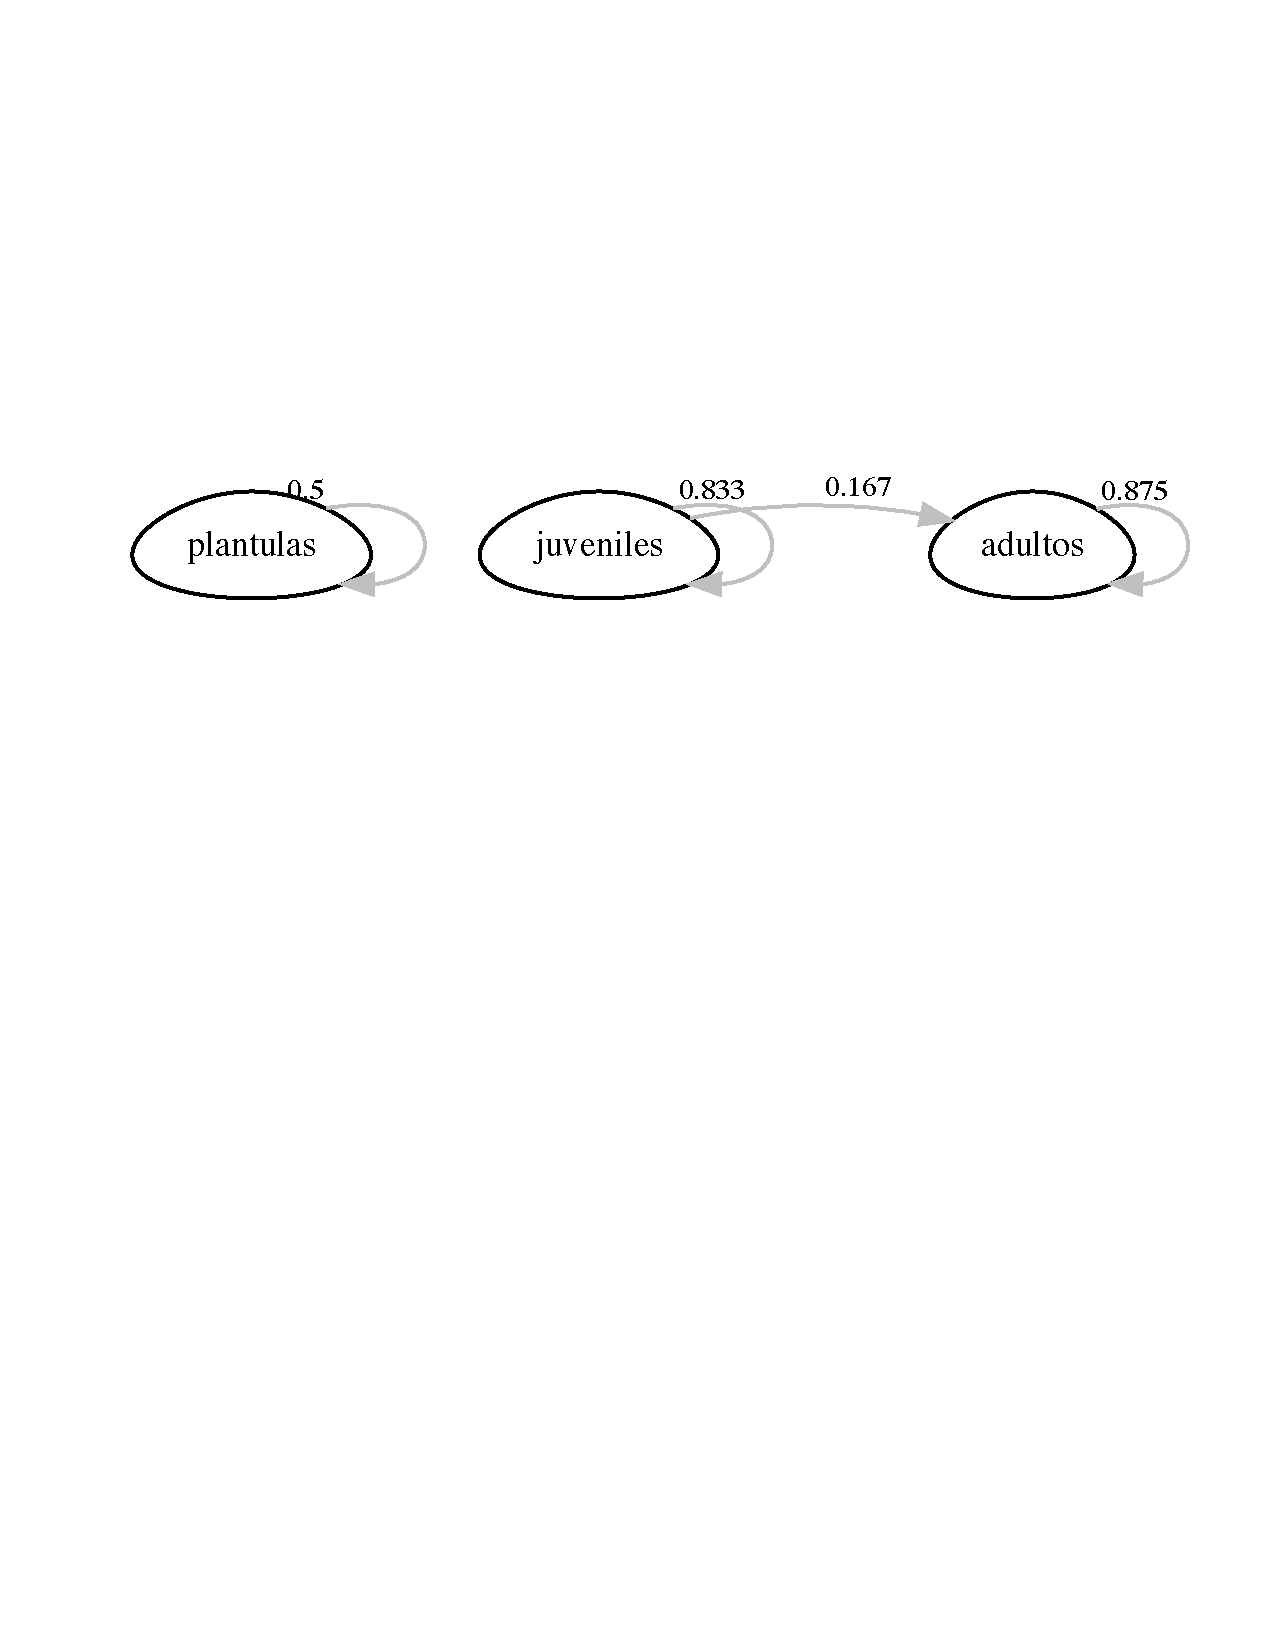
\includegraphics[keepaspectratio]{108-Bayesian_PPM_files/figure-pdf/bayes11-1.pdf}}

\begin{center}\rule{0.5\linewidth}{0.5pt}\end{center}

\subsection{Incorporar previas
informativas}\label{incorporar-previas-informativas}

Para evitar que el modelo genere transiciones imposibles entre etapas
del ciclo de vida, se pueden incorporar previas informativas. Estas
previas se basan en el conocimiento experto sobre la especie, en este
caso proporcionado por un especialista en orquídeas epífitas del género
\emph{Lepanthes} (RLT). La información debe tener el mismo formato que
la matriz de transición, es decir:

\begin{itemize}
\tightlist
\item
  Una matriz con una fila más que columnas.
\item
  La última fila representa los individuos que mueren en cada etapa.
\end{itemize}

Es importante que estos valores se definan antes de recolectar los datos
de campo, para evitar que el análisis se vea influenciado o sesgado por
los datos observados.

\begin{Shaded}
\begin{Highlighting}[]
\NormalTok{RLT\_Tprior }\OtherTok{\textless{}{-}} \FunctionTok{matrix}\NormalTok{(}\FunctionTok{c}\NormalTok{(}\FloatTok{0.25}\NormalTok{, }\FloatTok{0.025}\NormalTok{, }\FloatTok{0.0}\NormalTok{,}
                       \FloatTok{0.05}\NormalTok{, }\FloatTok{0.9}\NormalTok{,   }\FloatTok{0.025}\NormalTok{,}
                       \FloatTok{0.01}\NormalTok{, }\FloatTok{0.025}\NormalTok{, }\FloatTok{0.95}\NormalTok{,}
                       \FloatTok{0.69}\NormalTok{, }\FloatTok{0.05}\NormalTok{,  }\FloatTok{0.025}\NormalTok{), }
                       \AttributeTok{byrow =} \ConstantTok{TRUE}\NormalTok{, }\AttributeTok{nrow =} \DecValTok{4}\NormalTok{, }\AttributeTok{ncol =} \DecValTok{3}\NormalTok{)}
\end{Highlighting}
\end{Shaded}

Note que en la matriz, la 1ª fila, 3ª columna es 0.0, porque esta
transición es imposible. Las previas se construyen de manera que las
columnas sumen 1, lo que crea mayor flexibilidad para la ponderación de
los valores \emph{a priori}. Por defecto, la suma es 1, interpretado
como un \emph{tamaño de muestra a priori} de 1.

Ahora, usando la función \texttt{fill\_transitions} se agregan los
valores del campo \textbf{TF}, el tamaño de muestra en el tiempo inicial
\textbf{N}, la matriz de valores con \emph{priors} informativos, y se
calcula la matriz de transición \emph{a posteriori}. Compare \textbf{TF}
con esta matriz para ver los cambios.

\begin{Shaded}
\begin{Highlighting}[]
\FunctionTok{fill\_transitions}\NormalTok{(TF, N, }\AttributeTok{P =}\NormalTok{ RLT\_Tprior)}
\end{Highlighting}
\end{Shaded}

\begin{verbatim}
             [,1]         [,2]         [,3]
[1,] 0.1041666667 0.0005208333 0.0000000000
[2,] 0.5875000000 0.5812500000 0.0007142857
[3,] 0.0008333333 0.2921875000 0.8557142857
\end{verbatim}

\begin{center}\rule{0.5\linewidth}{0.5pt}\end{center}

\subsection{\texorpdfstring{Modificar el peso de los valores \emph{a
priori}}{Modificar el peso de los valores a priori}}\label{modificar-el-peso-de-los-valores-a-priori}

Cuando usamos previas informativas en el modelo, podemos ajustar su peso
para reflejar cuánto creemos en la previa frente a los datos. Esto se
hace con el argumento \texttt{priorweight} de
\texttt{fill\_transitions()}.

\textbf{¿Cómo funciona \texttt{priorweight} exactamente?} El argumento
es un \textbf{multiplicador sobre el tamaño de muestra observado} \(N\):

\begin{itemize}
\tightlist
\item
  La contribución efectiva de la previa = \texttt{priorweight} × \(N\)
  (en unidades de ``observaciones equivalentes'').
\item
  El tamaño de muestra efectivo total = \(N\) + \texttt{priorweight} ×
  \(N\) = \(N \times (1 + \text{priorweight})\).
\item
  Por defecto \texttt{priorweight\ =\ -1}, lo que hace que la previa
  contribuya solamente su suma original (típicamente 1, ya que cada
  columna de la matriz de previas se construye para sumar 1).
\end{itemize}

\begin{Shaded}
\begin{Highlighting}[]
\FunctionTok{fill\_transitions}\NormalTok{(TF, N, }\AttributeTok{P =}\NormalTok{ RLT\_Tprior, }\AttributeTok{priorweight =} \FloatTok{0.5}\NormalTok{)}
\end{Highlighting}
\end{Shaded}

\begin{verbatim}
            [,1]        [,2]        [,3]
[1,] 0.143939394 0.008333333 0.000000000
[2,] 0.440909091 0.682978723 0.008333333
[3,] 0.003333333 0.206914894 0.885294118
\end{verbatim}

\begin{tcolorbox}[enhanced jigsaw, arc=.35mm, bottomrule=.15mm, bottomtitle=1mm, breakable, colback=white, colbacktitle=quarto-callout-important-color!10!white, colframe=quarto-callout-important-color-frame, coltitle=black, left=2mm, leftrule=.75mm, opacityback=0, opacitybacktitle=0.6, rightrule=.15mm, title=\textcolor{quarto-callout-important-color}{\faExclamation}\hspace{0.5em}{Importante}, titlerule=0mm, toprule=.15mm, toptitle=1mm]

\textbf{El ``peso de la previa'' es un tamaño de muestra equivalente.}
Asignar \texttt{priorweight\ =\ 0.5} con \(N = 2\) observaciones es como
decir: ``antes de salir al campo, mi creencia tiene la misma fuerza que
\(0.5 \times 2 = 1\) observación adicional''. Si tu previa tiene peso
efectivo 5 y observas 50 transiciones, los datos pesarán 10 veces más
que la previa. La regla práctica es dejar que los datos dominen: el peso
de la previa debería ser \textbf{mucho menor} que el tamaño de muestra
observado, salvo que tengas razones biológicas muy fuertes para confiar
en la previa.

\end{tcolorbox}

Algunos valores típicos de \texttt{priorweight}:

\begin{itemize}
\tightlist
\item
  \texttt{priorweight\ =\ -1} (defecto): la previa contribuye su suma
  original, típicamente 1 observación equivalente. Útil como previa
  débil.
\item
  \texttt{priorweight\ =\ 0.1} a \texttt{0.5}: la previa pesa entre 10\%
  y 50\% del tamaño de muestra observado. Apropiado cuando hay
  conocimiento experto pero los datos deben dominar.
\item
  \texttt{priorweight\ =\ 1}: la previa pesa lo mismo que los datos.
  Sólo justificado si los datos son muy escasos y la previa es muy
  confiable.
\item
  \texttt{priorweight\ \textgreater{}\ 1}: la previa pesa más que los
  datos. Rara vez justificado en estudios poblacionales.
\end{itemize}

\begin{tcolorbox}[enhanced jigsaw, arc=.35mm, bottomrule=.15mm, bottomtitle=1mm, breakable, colback=white, colbacktitle=quarto-callout-warning-color!10!white, colframe=quarto-callout-warning-color-frame, coltitle=black, left=2mm, leftrule=.75mm, opacityback=0, opacitybacktitle=0.6, rightrule=.15mm, title=\textcolor{quarto-callout-warning-color}{\faExclamationTriangle}\hspace{0.5em}{Advertencia}, titlerule=0mm, toprule=.15mm, toptitle=1mm]

\textbf{Cuándo no usar una previa informativa fuerte.} Las previas
informativas son apropiadas cuando hay conocimiento biológico sólido que
no aparece en los datos (e.g., experiencia directa con la especie,
estudios en poblaciones cercanas). \textbf{No} son apropiadas cuando:

\begin{itemize}
\tightlist
\item
  El tamaño de muestra ya es grande y todas las transiciones se
  observaron varias veces --- la previa solo introduce sesgo.
\item
  No hay base experta para definir la previa --- usar valores
  ``razonables sin justificación'' es proyectar incertidumbre como si
  fuera conocimiento.
\item
  Se está comparando entre poblaciones --- usar la misma previa para
  todas puede borrar diferencias reales.
\end{itemize}

En estos casos, conviene usar previas débiles (poco peso) o reportar
resultados con y sin previa para mostrar la sensibilidad a la elección.

\end{tcolorbox}

\textbf{Recomendación general:} asigna a las previas un peso menor
(preferiblemente mucho menor) que el tamaño de muestra observado. Esto
garantiza que los datos reales tengan mayor peso en el análisis y evita
que el conocimiento previo domine injustamente los resultados.

\textbf{Resultado}

La nueva matriz de transición:

\begin{itemize}
\tightlist
\item
  Es ergódica (todas las etapas están conectadas directa o
  indirectamente).
\item
  Es reducible, lo que significa que algunas etapas pueden no ser
  alcanzables desde otras, dependiendo del ciclo de vida.
\item
  Presenta tasas de mortandad y transición más realistas, gracias a la
  incorporación del conocimiento experto.
\end{itemize}

\begin{center}\rule{0.5\linewidth}{0.5pt}\end{center}

\section{Intervalos de credibilidad para las
transiciones}\label{intervalos-de-credibilidad-para-las-transiciones}

Una vez ajustada la matriz de transición con los datos observados y las
previas informativas, podemos calcular los intervalos de credibilidad
(ICr) para cada entrada de la matriz.

\begin{tcolorbox}[enhanced jigsaw, arc=.35mm, bottomrule=.15mm, bottomtitle=1mm, breakable, colback=white, colbacktitle=quarto-callout-note-color!10!white, colframe=quarto-callout-note-color-frame, coltitle=black, left=2mm, leftrule=.75mm, opacityback=0, opacitybacktitle=0.6, rightrule=.15mm, title=\textcolor{quarto-callout-note-color}{\faInfo}\hspace{0.5em}{Nota}, titlerule=0mm, toprule=.15mm, toptitle=1mm]

\textbf{Por qué Dirichlet (transiciones) y Gamma (fecundidad).} Cada
columna de una matriz de transición es un vector de probabilidades que
suman 1. La distribución natural sobre tales vectores es la
\textbf{distribución Dirichlet}, generalización multidimensional de la
Beta. Al observar transiciones (datos multinomiales) y combinar con una
previa Dirichlet, la posterior \textbf{también es Dirichlet} (es una
previa conjugada) --- esto hace los cálculos exactos y rápidos. Para
cada entrada individual de la matriz, la distribución marginal es
\textbf{Beta}, lo cual permite calcular intervalos de credibilidad
directamente con \texttt{qbeta()}. La fecundidad, por ser un conteo
positivo no acotado, se modela con una previa \textbf{Gamma} sobre la
tasa de Poisson.

\end{tcolorbox}

\begin{tcolorbox}[enhanced jigsaw, arc=.35mm, bottomrule=.15mm, bottomtitle=1mm, breakable, colback=white, colbacktitle=quarto-callout-note-color!10!white, colframe=quarto-callout-note-color-frame, coltitle=black, left=2mm, leftrule=.75mm, opacityback=0, opacitybacktitle=0.6, rightrule=.15mm, title=\textcolor{quarto-callout-note-color}{\faInfo}\hspace{0.5em}{Nota}, titlerule=0mm, toprule=.15mm, toptitle=1mm]

\textbf{Intervalo de confianza (IC) versus intervalo de credibilidad
(ICr).} Aunque suenan parecidos, significan cosas distintas:

\begin{itemize}
\tightlist
\item
  \textbf{IC frecuentista al 95\%:} ``si repitiéramos este estudio
  infinitas veces, el 95\% de los intervalos calculados contendrían el
  valor verdadero''. No es una afirmación sobre el parámetro en este
  estudio.
\item
  \textbf{ICr bayesiano al 95\%:} ``dada la previa y los datos, hay un
  95\% de probabilidad de que el verdadero valor del parámetro esté en
  este intervalo''. Es una afirmación directa sobre el parámetro.
\end{itemize}

Lo que la mayoría de las personas \emph{intuitivamente quieren decir} al
leer un IC frecuentista es la interpretación bayesiana --- y los
intervalos de credibilidad son los que efectivamente se la dan.

\end{tcolorbox}

\textbf{¿Cómo se calculan?} Cada elemento de la matriz de transición
ajustada sigue una distribución beta, ya que proviene de una
distribución posterior marginal de una Dirichlet
(multinomial-Dirichlet). Esto permite calcular intervalos de
credibilidad para las tasas de transición.

Para obtener estos valores, se puede usar el tipo de retorno TN, que
proporciona:

\begin{itemize}
\tightlist
\item
  La estimación puntual.
\item
  El límite inferior del intervalo de credibilidad al 95\%.
\item
  El límite superior del intervalo de credibilidad al 95\%.
\end{itemize}

\subsection{Ejemplo: etapa de
plántula}\label{ejemplo-etapa-de-pluxe1ntula}

Supongamos que estamos analizando las transiciones desde la etapa de
plántula (s). Si el número de transiciones observadas es 2, y el peso de
las previas es 1, el tamaño de muestra efectivo es 3. Esto genera un
intervalo de credibilidad más amplio, reflejando la alta incertidumbre
en la estimación. Por ejemplo:

\begin{itemize}
\tightlist
\item
  La tasa de mortandad puntual es 0.31.
\item
  El intervalo de credibilidad al 95\% va de 0.096 a 0.585.
\end{itemize}

Este rango amplio indica que el mejor estimado es muy incierto, lo cual
es típico cuando se trabaja con tamaños de muestra pequeños.

\subsection{Interpretación}\label{interpretaciuxf3n}

Un intervalo de credibilidad amplio significa que hay mucha
incertidumbre en la estimación del parámetro. Esto resalta la
importancia de contar con:

\begin{itemize}
\tightlist
\item
  Más datos de campo.
\item
  Previas bien fundamentadas.
\item
  Un análisis cuidadoso del tamaño de muestra efectivo.
\end{itemize}

\begin{Shaded}
\begin{Highlighting}[]
\NormalTok{TN }\OtherTok{\textless{}{-}} \FunctionTok{fill\_transitions}\NormalTok{(}
\NormalTok{  TF,}
\NormalTok{  N,}
  \AttributeTok{P =}\NormalTok{ RLT\_Tprior,}
  \AttributeTok{priorweight =} \FloatTok{0.1}\NormalTok{,}
  \AttributeTok{returnType =} \StringTok{"TN"}
\NormalTok{)}
\NormalTok{a }\OtherTok{\textless{}{-}}\NormalTok{ TN[, }\DecValTok{1}\NormalTok{] }\CommentTok{\# cambie 1 a 2, 3 etc para obtener la distribución beta marginal de cada columna (etapa de vida).}
\NormalTok{b }\OtherTok{\textless{}{-}} \FunctionTok{sum}\NormalTok{(TN[, }\DecValTok{1}\NormalTok{]) }\SpecialCharTok{{-}}\NormalTok{ TN[, }\DecValTok{1}\NormalTok{] }\CommentTok{\# cambie 1 a 2, 3 etc para obtener la distribución beta marginal de cada columna.}
\NormalTok{p }\OtherTok{\textless{}{-}}\NormalTok{ a }\SpecialCharTok{/}\NormalTok{ (a }\SpecialCharTok{+}\NormalTok{ b)}
\NormalTok{lcl }\OtherTok{\textless{}{-}} \FunctionTok{qbeta}\NormalTok{(}\FloatTok{0.025}\NormalTok{, a, b) }\CommentTok{\# el valor 0.025 de la distribución beta}
\NormalTok{ucl }\OtherTok{\textless{}{-}} \FunctionTok{qbeta}\NormalTok{(}\FloatTok{0.975}\NormalTok{, a, b) }\CommentTok{\# el valor 0.975 de la distribución beta}
\NormalTok{knitr}\SpecialCharTok{::}\FunctionTok{kable}\NormalTok{(}\FunctionTok{sprintf}\NormalTok{(}\StringTok{"\%.4f (\%.4f, \%.4f)"}\NormalTok{, p, lcl, ucl)) }\CommentTok{\# Crear una tabla con los resultados con 4 cifras decimales (note la ultima fila son los fallecidos)}
\end{Highlighting}
\end{Shaded}

{\def\LTcaptype{none} % do not increment counter
\begin{longtable}[]{@{}l@{}}
\toprule\noalign{}
x \\
\midrule\noalign{}
\endhead
\bottomrule\noalign{}
\endlastfoot
0.1054 (0.0058, 0.3212) \\
0.5831 (0.3087, 0.8315) \\
0.0009 (0.0000, 0.0052) \\
0.3107 (0.0956, 0.5846) \\
\end{longtable}
}

Una de las grandes ventajas de usar el paquete \texttt{raretrans} es que
podemos calcular los intervalos de credibilidad de las tasas de
transición y fecundidad de manera rápida y sencilla. Además, los
intervalos de credibilidad están limitados a los valores entre 0 y 1, lo
que es importante para las tasas de transición y fecundidad. Esto es
especialmente útil cuando se trabaja con datos de campo donde el tamaño
de muestra es pequeño y las transiciones raras son comunes. Muchos
métodos estadísticos no pueden calcular intervalos de confianza para
tasas de transición y fecundidad, y cuando lo hacen tienen valores
ilógicos, como proporciones negativas o mayores a 1.

\begin{center}\rule{0.5\linewidth}{0.5pt}\end{center}

\subsection{El efecto del tamaño de muestra sobre los intervalos de
credibilidad}\label{el-efecto-del-tamauxf1o-de-muestra-sobre-los-intervalos-de-credibilidad}

Cuando se aumenta el \textbf{tamaño de muestra efectivo}, los
\textbf{intervalos de credibilidad} se vuelven más estrechos, lo que
indica mayor confianza en las estimaciones puntuales. Aumentar el tamaño
de muestra efectivo a \(20\) especificando:
\texttt{priorweight}\(= 9 (9*2 = 18 + 2 = 20)\) hace que los intervalos
de credibilidad se reduzcan bastante. Entonces, es importante enfatizar
en que el tamaño de muestra tiene gran impacto sobre la confianza que se
tiene sobre el estimador puntual (el promedio) de las transiciones,
permanencias y mortalidad. Note en la figura como el tamaño del
intervalo de credibilidad cambia drásticamente cuando se aumenta el
número de datos.

El intervalo de credibilidad se estrecha cuando el tamaño de muestra
efectivo aumenta, reflejando mayor confianza en el estimador puntual.

IMPORTANTE: Aunque este ejemplo muestra cómo el tamaño de muestra afecta
la credibilidad, en la práctica:

\begin{itemize}
\tightlist
\item
  El peso de las previas (priorweight) debe ser menor que el tamaño de
  muestra observado.
\item
  Esto asegura que los datos reales del campo tengan mayor influencia en
  el análisis.
\item
  Usar un tamaño de muestra a priori demasiado grande puede sesgar los
  resultados y reducir la validez del modelo.
\end{itemize}

\begin{Shaded}
\begin{Highlighting}[]
\NormalTok{TN }\OtherTok{\textless{}{-}} \FunctionTok{fill\_transitions}\NormalTok{(}
\NormalTok{  TF,}
\NormalTok{  N,}
  \AttributeTok{P =}\NormalTok{ RLT\_Tprior,}
  \AttributeTok{priorweight =} \DecValTok{9}\NormalTok{,}
  \AttributeTok{returnType =} \StringTok{"TN"}
\NormalTok{)}
\NormalTok{a }\OtherTok{\textless{}{-}}\NormalTok{ TN[, }\DecValTok{1}\NormalTok{]}
\NormalTok{b }\OtherTok{\textless{}{-}} \FunctionTok{sum}\NormalTok{(TN[, }\DecValTok{1}\NormalTok{]) }\SpecialCharTok{{-}}\NormalTok{ TN[, }\DecValTok{1}\NormalTok{] }\CommentTok{\# El parámetro beta es la suma de todos los demás parámetros de Dirichlet.}
\NormalTok{p2 }\OtherTok{\textless{}{-}}\NormalTok{ a }\SpecialCharTok{/}\NormalTok{ (a }\SpecialCharTok{+}\NormalTok{ b)}
\NormalTok{lcl2 }\OtherTok{\textless{}{-}} \FunctionTok{qbeta}\NormalTok{(}\FloatTok{0.025}\NormalTok{, a, b)}
\NormalTok{ucl2 }\OtherTok{\textless{}{-}} \FunctionTok{qbeta}\NormalTok{(}\FloatTok{0.975}\NormalTok{, a, b)}
\NormalTok{alltogethernow }\OtherTok{\textless{}{-}} \FunctionTok{tibble}\NormalTok{(}
  \AttributeTok{priorweight =} \FunctionTok{factor}\NormalTok{(}\FunctionTok{rep}\NormalTok{(}\FunctionTok{c}\NormalTok{(}\DecValTok{1}\NormalTok{, }\DecValTok{9}\NormalTok{), }\AttributeTok{each =} \DecValTok{4}\NormalTok{)),}
  \AttributeTok{fate =} \FunctionTok{factor}\NormalTok{(}
    \FunctionTok{rep}\NormalTok{(}\FunctionTok{c}\NormalTok{(}\StringTok{"s"}\NormalTok{, }\StringTok{"j"}\NormalTok{, }\StringTok{"a"}\NormalTok{, }\StringTok{"dead"}\NormalTok{), }\AttributeTok{times =} \DecValTok{2}\NormalTok{),}
    \AttributeTok{levels =} \FunctionTok{c}\NormalTok{(}\StringTok{"s"}\NormalTok{, }\StringTok{"j"}\NormalTok{, }\StringTok{"a"}\NormalTok{, }\StringTok{"dead"}\NormalTok{)}
\NormalTok{  ),}
  \AttributeTok{p =} \FunctionTok{c}\NormalTok{(p, p2),}
  \AttributeTok{lcl =} \FunctionTok{c}\NormalTok{(lcl, lcl2),}
  \AttributeTok{ucl =} \FunctionTok{c}\NormalTok{(ucl, ucl2)}
\NormalTok{)}
\FunctionTok{ggplot}\NormalTok{(}
  \AttributeTok{data =}\NormalTok{ alltogethernow,}
  \AttributeTok{mapping =} \FunctionTok{aes}\NormalTok{(}\AttributeTok{x =}\NormalTok{ fate, }\AttributeTok{y =}\NormalTok{ p, }\AttributeTok{group =}\NormalTok{ priorweight, }\AttributeTok{colour =}\NormalTok{ priorweight)}
\NormalTok{) }\SpecialCharTok{+}
  \FunctionTok{geom\_point}\NormalTok{(}
    \AttributeTok{mapping =} \FunctionTok{aes}\NormalTok{(}\AttributeTok{shape =}\NormalTok{ priorweight),}
    \AttributeTok{position =} \FunctionTok{position\_dodge}\NormalTok{(}\AttributeTok{width =} \FloatTok{0.5}\NormalTok{)}
\NormalTok{  ) }\SpecialCharTok{+}
  \FunctionTok{geom\_errorbar}\NormalTok{(}
    \AttributeTok{mapping =} \FunctionTok{aes}\NormalTok{(}\AttributeTok{ymin =}\NormalTok{ lcl, }\AttributeTok{ymax =}\NormalTok{ ucl),}
    \AttributeTok{position =} \FunctionTok{position\_dodge}\NormalTok{(}\AttributeTok{width =} \FloatTok{0.5}\NormalTok{)}
\NormalTok{  ) }\SpecialCharTok{+}
  \FunctionTok{theme\_bw}\NormalTok{() }\SpecialCharTok{+}
  \FunctionTok{rlt\_style\_colour}\NormalTok{()}
\end{Highlighting}
\end{Shaded}

\pandocbounded{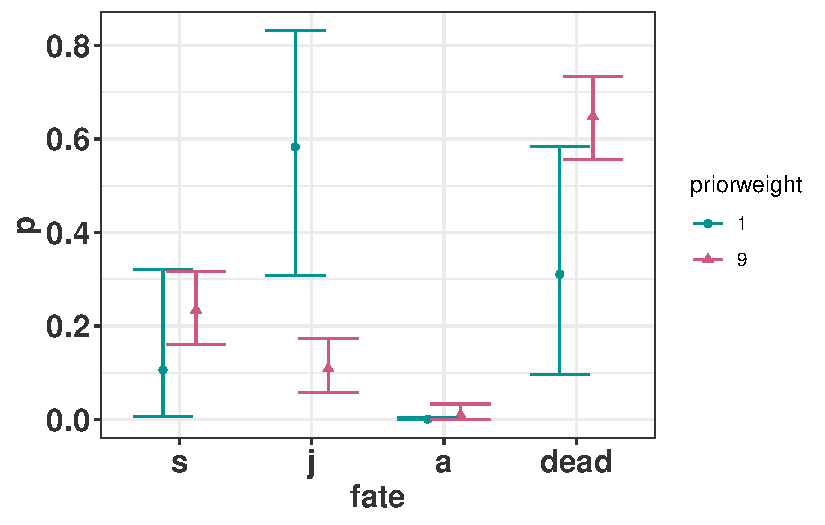
\includegraphics[keepaspectratio]{108-Bayesian_PPM_files/figure-pdf/bayes16-1.pdf}}

\begin{center}\rule{0.5\linewidth}{0.5pt}\end{center}

\section{\texorpdfstring{Intervalo de credibilidad para la tasa de
crecimiento asintótica
\(\lambda\)}{Intervalo de credibilidad para la tasa de crecimiento asintótica \textbackslash lambda}}\label{intervalo-de-credibilidad-para-la-tasa-de-crecimiento-asintuxf3tica-lambda}

Obtener intervalos de credibilidad para la tasa de crecimiento
asintótica, \(\lambda\), requiere simular matrices a partir de las
distribuciones posteriores. Estas simulaciones usualmente son
complicadas de hacer, por lo que hemos incorporado en el paquete la
función \texttt{raretrans::sim\_transitions()} para generar una lista de
matrices simuladas dada la matriz observada y las previas. En otras
palabras, esta función calcula múltiples veces las matrices de
transición y fecundidad basándose en los datos observados y en los
valores \emph{a priori} especificados, pero variando los valores de los
parámetros de las distribuciones beta y gamma.

\subsection{Simulación de una matriz de
transición}\label{simulaciuxf3n-de-una-matriz-de-transiciuxf3n}

Siguiendo el marco bayesiano que hemos venido trabajando en este
capítulo, es necesario especificar las previas de la fecundidad como una
matriz. Las celdas de la matriz de los estados en los que no hay
reproducción deben ser \texttt{NA}, usando \texttt{NA\_real\_}, el cual
es un valor que no está presente pero podría aceptar valores con puntos
decimales. Nota que el valor \emph{a priori} de la fecundidad es 0.0001.

\begin{Shaded}
\begin{Highlighting}[]
\NormalTok{alpha }\OtherTok{\textless{}{-}} \FunctionTok{matrix}\NormalTok{(}\FunctionTok{c}\NormalTok{(}\ConstantTok{NA\_real\_}\NormalTok{, }\ConstantTok{NA\_real\_}\NormalTok{, }\FloatTok{1e{-}5}\NormalTok{,}
                  \ConstantTok{NA\_real\_}\NormalTok{, }\ConstantTok{NA\_real\_}\NormalTok{, }\ConstantTok{NA\_real\_}\NormalTok{,}
                  \ConstantTok{NA\_real\_}\NormalTok{, }\ConstantTok{NA\_real\_}\NormalTok{, }\ConstantTok{NA\_real\_}\NormalTok{), }\AttributeTok{nrow=}\DecValTok{3}\NormalTok{, }\AttributeTok{ncol =} \DecValTok{3}\NormalTok{, }\AttributeTok{byrow =} \ConstantTok{TRUE}\NormalTok{)}

\NormalTok{beta }\OtherTok{\textless{}{-}} \FunctionTok{matrix}\NormalTok{(}\FunctionTok{c}\NormalTok{(}\ConstantTok{NA\_real\_}\NormalTok{, }\ConstantTok{NA\_real\_}\NormalTok{, }\FloatTok{1e{-}5}\NormalTok{,}
                 \ConstantTok{NA\_real\_}\NormalTok{, }\ConstantTok{NA\_real\_}\NormalTok{, }\ConstantTok{NA\_real\_}\NormalTok{,}
                 \ConstantTok{NA\_real\_}\NormalTok{, }\ConstantTok{NA\_real\_}\NormalTok{, }\ConstantTok{NA\_real\_}\NormalTok{), }\AttributeTok{nrow=}\DecValTok{3}\NormalTok{, }\AttributeTok{ncol =} \DecValTok{3}\NormalTok{, }\AttributeTok{byrow =} \ConstantTok{TRUE}\NormalTok{)}

\FunctionTok{fill\_fertility}\NormalTok{(TF, N, }\AttributeTok{alpha =}\NormalTok{ alpha, }\AttributeTok{beta =}\NormalTok{ beta)}
\end{Highlighting}
\end{Shaded}

\begin{verbatim}
   
            s         j         a
  s 0.0000000 0.0000000 0.1176473
  j 0.0000000 0.0000000 0.0000000
  a 0.0000000 0.0000000 0.0000000
\end{verbatim}

El cambio en la fecundidad es \textless{} 0.0001 en comparación con el
valor observado.

\subsection{Una simulación de la matriz de
transición}\label{una-simulaciuxf3n-de-la-matriz-de-transiciuxf3n}

Corra el script múltiples veces, y verá que los valores cambian en cada
simulación. En este script la simulación es solamente una vez
(\texttt{samples\ =\ 1}). Este script es para que visualicen lo que hace
la función \texttt{sim\_transitions()}.

\begin{Shaded}
\begin{Highlighting}[]
\FunctionTok{sim\_transitions}\NormalTok{(}
\NormalTok{  TF,}
\NormalTok{  N,}
  \AttributeTok{P =}\NormalTok{ RLT\_Tprior,}
  \AttributeTok{alpha =}\NormalTok{ alpha,}
  \AttributeTok{beta =}\NormalTok{ beta,}
  \AttributeTok{priorweight =} \FloatTok{0.5}\NormalTok{,}
  \AttributeTok{samples =} \DecValTok{1}
\NormalTok{)}
\end{Highlighting}
\end{Shaded}

\begin{verbatim}
[[1]]
             [,1]       [,2]       [,3]
[1,] 8.477944e-02 0.04726174 0.36643080
[2,] 6.356950e-01 0.68519207 0.02394929
[3,] 1.786360e-11 0.11711938 0.85899290
\end{verbatim}

\subsection{Simulación de 5000 matrices de
transición}\label{simulaciuxf3n-de-5000-matrices-de-transiciuxf3n}

Ahora simulamos 5000 veces, calculamos el valor \(\lambda\) de cada
matriz y creamos un histograma de su distribución. Se añaden los valores
de lambda en un objeto llamado \texttt{RLT\_0.5}. Se visualiza la
distribución de \(\lambda\) usando un histograma. Note que el valor de
\(\lambda = 1\) queda dentro de la distribución; en otras palabras, el
histograma muestra que la mayoría de los valores de \(\lambda\) están
cerca de 1.

\begin{Shaded}
\begin{Highlighting}[]
\CommentTok{\#set.seed(8390278) \# make this part reproducible}
\NormalTok{alpha2 }\OtherTok{\textless{}{-}} \FunctionTok{matrix}\NormalTok{(}\FunctionTok{c}\NormalTok{(}\ConstantTok{NA\_real\_}\NormalTok{, }\ConstantTok{NA\_real\_}\NormalTok{, }\FloatTok{0.025}\NormalTok{,}
                   \ConstantTok{NA\_real\_}\NormalTok{, }\ConstantTok{NA\_real\_}\NormalTok{, }\ConstantTok{NA\_real\_}\NormalTok{,}
                   \ConstantTok{NA\_real\_}\NormalTok{, }\ConstantTok{NA\_real\_}\NormalTok{, }\ConstantTok{NA\_real\_}\NormalTok{), }\AttributeTok{nrow=}\DecValTok{3}\NormalTok{, }\AttributeTok{ncol =} \DecValTok{3}\NormalTok{, }\AttributeTok{byrow =} \ConstantTok{TRUE}\NormalTok{)}

\NormalTok{beta2 }\OtherTok{\textless{}{-}} \FunctionTok{matrix}\NormalTok{(}\FunctionTok{c}\NormalTok{(}\ConstantTok{NA\_real\_}\NormalTok{, }\ConstantTok{NA\_real\_}\NormalTok{, }\DecValTok{1}\NormalTok{,}
                  \ConstantTok{NA\_real\_}\NormalTok{, }\ConstantTok{NA\_real\_}\NormalTok{, }\ConstantTok{NA\_real\_}\NormalTok{,}
                  \ConstantTok{NA\_real\_}\NormalTok{, }\ConstantTok{NA\_real\_}\NormalTok{, }\ConstantTok{NA\_real\_}\NormalTok{), }\AttributeTok{nrow=}\DecValTok{3}\NormalTok{, }\AttributeTok{ncol =} \DecValTok{3}\NormalTok{, }\AttributeTok{byrow =} \ConstantTok{TRUE}\NormalTok{)}

\CommentTok{\# generar 5000 matrices basadas en las previas de transiciones y de fecundidades, el tamaño de muestra, además de los datos}
\NormalTok{RLT\_0}\FloatTok{.5}\NormalTok{s }\OtherTok{\textless{}{-}} \FunctionTok{sim\_transitions}\NormalTok{(TF, N, }\AttributeTok{P =}\NormalTok{ RLT\_Tprior, }\AttributeTok{alpha =}\NormalTok{ alpha2, }\AttributeTok{beta =}\NormalTok{ beta2,}
                \AttributeTok{priorweight =} \FloatTok{0.5}\NormalTok{, }\AttributeTok{samples =} \DecValTok{5000}\NormalTok{)}

\CommentTok{\# extraer los valores de lambda de cada simulación en un histograma}

\NormalTok{RLT\_0}\FloatTok{.5} \OtherTok{\textless{}{-}} \FunctionTok{tibble}\NormalTok{(}\AttributeTok{lposterior =} \FunctionTok{map\_dbl}\NormalTok{(RLT\_0}\FloatTok{.5}\NormalTok{s, lambda)) }\CommentTok{\# convertir la lista en un tibble}
\FunctionTok{ggplot}\NormalTok{(}\AttributeTok{data =}\NormalTok{ RLT\_0}\FloatTok{.5}\NormalTok{,}
       \AttributeTok{mapping =} \FunctionTok{aes}\NormalTok{(}\AttributeTok{x =}\NormalTok{ lposterior)) }\SpecialCharTok{+} 
  \FunctionTok{geom\_histogram}\NormalTok{(}\AttributeTok{binwidth =} \FloatTok{0.01}\NormalTok{, }\AttributeTok{colour=}\StringTok{"white"}\NormalTok{) }\SpecialCharTok{+} 
  \FunctionTok{theme\_bw}\NormalTok{() }\SpecialCharTok{+}
  \FunctionTok{rlt\_style\_fill}\NormalTok{() }\SpecialCharTok{+}
  \FunctionTok{geom\_vline}\NormalTok{(}\AttributeTok{xintercept =} \DecValTok{1}\NormalTok{, }
                \AttributeTok{color =} \StringTok{"\#009392"}\NormalTok{, }\AttributeTok{linewidth=}\FloatTok{1.5}\NormalTok{)}
\end{Highlighting}
\end{Shaded}

\pandocbounded{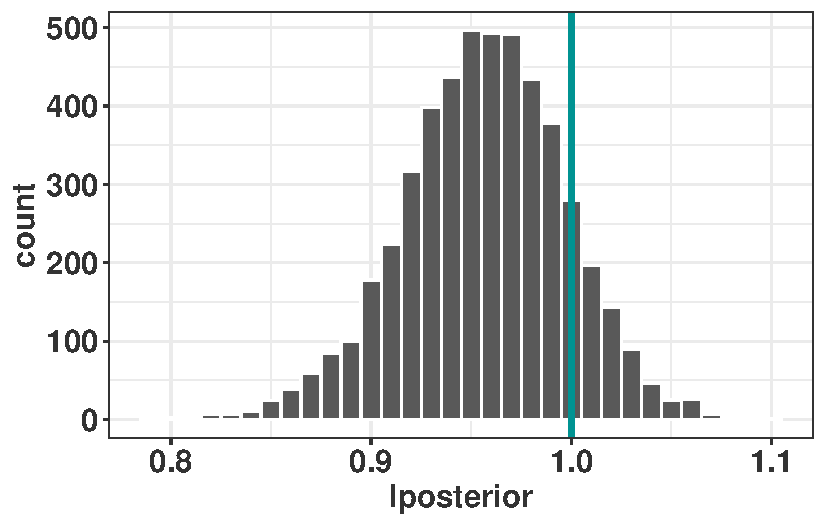
\includegraphics[keepaspectratio]{108-Bayesian_PPM_files/figure-pdf/bayes19-1.pdf}}

\begin{center}\rule{0.5\linewidth}{0.5pt}\end{center}

\section{Probabilidad posterior de que la población esté creciendo (λ
\textgreater{}
1)}\label{probabilidad-posterior-de-que-la-poblaciuxf3n-estuxe9-creciendo-ux3bb-1}

A diferencia de un contraste de hipótesis frecuentista (donde se obtiene
un valor-p), el marco bayesiano nos permite responder directamente la
pregunta de interés: \textbf{¿con qué probabilidad la población está
creciendo?} Lo hacemos contando qué proporción de las simulaciones de la
distribución posterior produjo \(\lambda > 1\). En este caso,
\(P(\lambda > 1 \mid \text{datos}, \text{previas}) = 0.14\), lo que
indica que sólo en el 14\% de los escenarios consistentes con los datos
y la previa la población crece. La evidencia para crecimiento
poblacional es débil; lo más probable es que la población esté en
declive. La estadística \texttt{p\_increase} reporta exactamente este
valor.

\begin{Shaded}
\begin{Highlighting}[]
\NormalTok{RLT\_0}\FloatTok{.5}\NormalTok{\_summary }\OtherTok{\textless{}{-}} \FunctionTok{summarize}\NormalTok{(}
\NormalTok{  RLT\_0}\FloatTok{.5}\NormalTok{,}
  \AttributeTok{medianaL =} \FunctionTok{median}\NormalTok{(lposterior),}
  \AttributeTok{promedioL =} \FunctionTok{mean}\NormalTok{(lposterior),}
  \AttributeTok{skewnessL=}\NormalTok{e1071}\SpecialCharTok{::}\FunctionTok{skewness}\NormalTok{(lposterior, }\AttributeTok{type=}\DecValTok{2}\NormalTok{),}
  \AttributeTok{ICrBajo =} \FunctionTok{quantile}\NormalTok{(lposterior, }\AttributeTok{probs =} \FloatTok{0.025}\NormalTok{),}
  \AttributeTok{ICrAlto =} \FunctionTok{quantile}\NormalTok{(lposterior, }\AttributeTok{probs =} \FloatTok{0.975}\NormalTok{),}
  \AttributeTok{p\_increase =} \FunctionTok{sum}\NormalTok{(lposterior }\SpecialCharTok{\textgreater{}} \FloatTok{1.}\NormalTok{) }\SpecialCharTok{/} \FunctionTok{n}\NormalTok{()}
\NormalTok{)}
\end{Highlighting}
\end{Shaded}

\subsection{Tabla de resultado de
lambda}\label{tabla-de-resultado-de-lambda}

\begin{Shaded}
\begin{Highlighting}[]
\FunctionTok{flextable}\NormalTok{(}\FunctionTok{signif}\NormalTok{(RLT\_0}\FloatTok{.5}\NormalTok{\_summary, }\AttributeTok{digits =} \DecValTok{2}\NormalTok{))}
\end{Highlighting}
\end{Shaded}

\global\setlength{\Oldarrayrulewidth}{\arrayrulewidth}

\global\setlength{\Oldtabcolsep}{\tabcolsep}

\setlength{\tabcolsep}{2pt}

\renewcommand*{\arraystretch}{1.5}



\providecommand{\ascline}[3]{\noalign{\global\arrayrulewidth #1}\arrayrulecolor[HTML]{#2}\cline{#3}}

\begin{longtable*}[c]{cccccc}



\ascline{1.5pt}{666666}{1-6}

\multicolumn{1}{>{}r}{\textcolor[HTML]{000000}{\fontsize{11}{11}\selectfont{medianaL}}} & \multicolumn{1}{>{}r}{\textcolor[HTML]{000000}{\fontsize{11}{11}\selectfont{promedioL}}} & \multicolumn{1}{>{}r}{\textcolor[HTML]{000000}{\fontsize{11}{11}\selectfont{skewnessL}}} & \multicolumn{1}{>{}r}{\textcolor[HTML]{000000}{\fontsize{11}{11}\selectfont{ICrBajo}}} & \multicolumn{1}{>{}r}{\textcolor[HTML]{000000}{\fontsize{11}{11}\selectfont{ICrAlto}}} & \multicolumn{1}{>{}r}{\textcolor[HTML]{000000}{\fontsize{11}{11}\selectfont{p\_increase}}} \\

\ascline{1.5pt}{666666}{1-6}\endfirsthead 

\ascline{1.5pt}{666666}{1-6}

\multicolumn{1}{>{}r}{\textcolor[HTML]{000000}{\fontsize{11}{11}\selectfont{medianaL}}} & \multicolumn{1}{>{}r}{\textcolor[HTML]{000000}{\fontsize{11}{11}\selectfont{promedioL}}} & \multicolumn{1}{>{}r}{\textcolor[HTML]{000000}{\fontsize{11}{11}\selectfont{skewnessL}}} & \multicolumn{1}{>{}r}{\textcolor[HTML]{000000}{\fontsize{11}{11}\selectfont{ICrBajo}}} & \multicolumn{1}{>{}r}{\textcolor[HTML]{000000}{\fontsize{11}{11}\selectfont{ICrAlto}}} & \multicolumn{1}{>{}r}{\textcolor[HTML]{000000}{\fontsize{11}{11}\selectfont{p\_increase}}} \\

\ascline{1.5pt}{666666}{1-6}\endhead



\multicolumn{1}{>{}r}{\textcolor[HTML]{000000}{\fontsize{11}{11}\selectfont{0.96}}} & \multicolumn{1}{>{}r}{\textcolor[HTML]{000000}{\fontsize{11}{11}\selectfont{0.96}}} & \multicolumn{1}{>{}r}{\textcolor[HTML]{000000}{\fontsize{11}{11}\selectfont{-0.26}}} & \multicolumn{1}{>{}r}{\textcolor[HTML]{000000}{\fontsize{11}{11}\selectfont{0.87}}} & \multicolumn{1}{>{}r}{\textcolor[HTML]{000000}{\fontsize{11}{11}\selectfont{1}}} & \multicolumn{1}{>{}r}{\textcolor[HTML]{000000}{\fontsize{11}{11}\selectfont{0.14}}} \\

\ascline{1.5pt}{666666}{1-6}



\end{longtable*}



\arrayrulecolor[HTML]{000000}

\global\setlength{\arrayrulewidth}{\Oldarrayrulewidth}

\global\setlength{\tabcolsep}{\Oldtabcolsep}

\renewcommand*{\arraystretch}{1}

\begin{center}\rule{0.5\linewidth}{0.5pt}\end{center}

\section{ADDENDUM}\label{addendum}

\begin{tcolorbox}[enhanced jigsaw, arc=.35mm, bottomrule=.15mm, bottomtitle=1mm, breakable, colback=white, colbacktitle=quarto-callout-important-color!10!white, colframe=quarto-callout-important-color-frame, coltitle=black, left=2mm, leftrule=.75mm, opacityback=0, opacitybacktitle=0.6, rightrule=.15mm, title=\textcolor{quarto-callout-important-color}{\faExclamation}\hspace{0.5em}{Importante}, titlerule=0mm, toprule=.15mm, toptitle=1mm]

\textbf{Nunca uses previas uniformes en análisis poblacionales reales.}
Una previa uniforme (e.g., Dirichlet con todos los parámetros iguales)
asigna la misma probabilidad a transiciones biológicamente plausibles y
a transiciones imposibles (un adulto reproductivo ``regresando'' a
plántula, una ballena bebé pasando directamente a madre, una semilla
transformándose en árbol adulto en un periodo). El resultado es una
matriz matemáticamente válida pero \textbf{biológicamente sin sentido},
que infla la incertidumbre con escenarios irreales y puede ocultar
señales legítimas en los datos.

\textbf{Siempre construye previas informadas} que reflejen el ciclo de
vida de la especie: marca con 0 las transiciones imposibles, asigna
probabilidades pequeñas a las raras pero posibles, y concentra masa en
las transiciones que la biología espera. La regla práctica es: si no
puedes defender la previa frente a un especialista de la especie, no la
uses.

La sección que sigue muestra qué pasa con una previa uniforme
\textbf{únicamente con fines didácticos} --- para que se vea de primera
mano por qué falla. No la copies en un análisis de tu propia especie.

\end{tcolorbox}

\subsection{Uso de previas uniformes}\label{uso-de-previas-uniformes}

Esta sección es para demostrar por qué no es recomendable el uso de
distribuciones previas uniformes. Si se entiende el concepto de valores
\emph{a priori} y \emph{a posteriori}, no es necesario leer esta
sección.

\subsection{Matriz de transición}\label{matriz-de-transiciuxf3n}

A continuación vamos a añadir una distribución Dirichlet uniforme como
previa con un peso = \(1\) a la matriz de transición, \(T\). En este
caso, tenemos 4 destinos (3 + muerte), por lo que cada destino añade
0.25 a la matriz de destinos \emph{observados} (¡no a la matriz de
transición!). Cuando especificamos una matriz con valores \emph{a
priori} para las transiciones, hay una fila más que columnas. Esta fila
extra representa la mortalidad por etapa.

Note que no se recomienda el uso de una previa uniforme; aquí se utiliza
sólo para mostrar el concepto. Una distribución previa uniforme no
refleja un ciclo de vida razonable para especies biológicas. Por
ejemplo, una previa uniforme podría hacer que las plántulas pasen a
adulto de un tiempo a otro o que los adultos regresen a ser plántulas,
lo cual no tiene mucho sentido biológico en muchas especies. Considera
lo siguiente: ¿es posible que una ballena bebé pueda pasar a ser madre
al año siguiente? Añadir una transición de 0.25 de ballena bebé a madre
no tiene sentido biológico.

Note que ahora la matriz de transición es ergódica pero no tiene sentido
biológico. Compare la matriz con las previas uniformes versus la matriz
original.

\begin{Shaded}
\begin{Highlighting}[]
\NormalTok{Tprior }\OtherTok{\textless{}{-}} \FunctionTok{matrix}\NormalTok{(}\FloatTok{0.25}\NormalTok{, }\AttributeTok{byrow =} \ConstantTok{TRUE}\NormalTok{, }\AttributeTok{ncol =} \DecValTok{3}\NormalTok{, }\AttributeTok{nrow =} \DecValTok{4}\NormalTok{) }\CommentTok{\# crear la matriz de previas uniformes}

\NormalTok{Tprior}
\end{Highlighting}
\end{Shaded}

\begin{verbatim}
     [,1] [,2] [,3]
[1,] 0.25 0.25 0.25
[2,] 0.25 0.25 0.25
[3,] 0.25 0.25 0.25
[4,] 0.25 0.25 0.25
\end{verbatim}

\begin{Shaded}
\begin{Highlighting}[]
\NormalTok{Posterior\_con\_Unif }\OtherTok{=} \FunctionTok{fill\_transitions}\NormalTok{(TF, N, }\AttributeTok{P =}\NormalTok{ Tprior) }\CommentTok{\# resultado de la matriz de transición básica con las previas}

\NormalTok{Posterior\_con\_Unif}
\end{Highlighting}
\end{Shaded}

\begin{verbatim}
           [,1]        [,2]        [,3]
[1,] 0.10416667 0.005208333 0.007142857
[2,] 0.60416667 0.567708333 0.007142857
[3,] 0.02083333 0.296875000 0.835714286
\end{verbatim}

\begin{Shaded}
\begin{Highlighting}[]
\CommentTok{\# Para entender las diferencias del impacto de las matriz compara los resultados con *$T* del objeto *TF*}
\NormalTok{TF}
\end{Highlighting}
\end{Shaded}

\begin{verbatim}
$T
   
             s          j          a
  s 0.09090909 0.00000000 0.00000000
  j 0.63636364 0.57446809 0.00000000
  a 0.00000000 0.29787234 0.85294118

$F
   
            s         j         a
  s 0.0000000 0.0000000 0.1176471
  j 0.0000000 0.0000000 0.0000000
  a 0.0000000 0.0000000 0.0000000
\end{verbatim}

\begin{center}\rule{0.5\linewidth}{0.5pt}\end{center}

\subsection{¿Cómo calcular en forma directa las transiciones de
estados?}\label{cuxf3mo-calcular-en-forma-directa-las-transiciones-de-estados}

Podemos obtener el resultado haciendo los cálculos directamente. Lo
primero que necesitamos es el vector de observaciones porque la
distribución posterior se calcula a partir de las observaciones de
transiciones, no de la matriz de transiciones. Si no tiene experiencia
con análisis Bayesiano es recomendable seguir los siguientes scripts

\begin{Shaded}
\begin{Highlighting}[]
\NormalTok{Tobs }\OtherTok{\textless{}{-}} \FunctionTok{sweep}\NormalTok{(TF}\SpecialCharTok{$}\NormalTok{T, }\DecValTok{2}\NormalTok{, N, }\StringTok{"*"}\NormalTok{) }\CommentTok{\# obtener las observaciones de transiciones}
\NormalTok{Tobs }\OtherTok{\textless{}{-}} \FunctionTok{rbind}\NormalTok{(Tobs, N }\SpecialCharTok{{-}} \FunctionTok{colSums}\NormalTok{(Tobs)) }\CommentTok{\# añadir la fila de muerte}
\NormalTok{Tobs }\OtherTok{\textless{}{-}}\NormalTok{ Tobs }\SpecialCharTok{+} \FloatTok{0.25} \CommentTok{\# añadir los valores de las previas}
\FunctionTok{sweep}\NormalTok{(Tobs, }\DecValTok{2}\NormalTok{, }\FunctionTok{colSums}\NormalTok{(Tobs), }\StringTok{"/"}\NormalTok{)[}\SpecialCharTok{{-}}\DecValTok{4}\NormalTok{, ] }\CommentTok{\# dividir por la suma de la columna y descarta la fila de muerte}
\end{Highlighting}
\end{Shaded}

\begin{verbatim}
           s           j           a
s 0.10416667 0.005208333 0.007142857
j 0.60416667 0.567708333 0.007142857
a 0.02083333 0.296875000 0.835714286
\end{verbatim}

La previa uniforme ``rellena'' las transiciones faltantes, pero también
crea problemas porque algunos de los valores de transición que se
asignan son biológicamente imposibles en muchas especies. Por ejemplo,
para la transición de adulto a plántula se asigna un valor; sin embargo,
este valor sólo es posible en la matriz de fecundidad \(F\) en las
especies de \emph{Lepanthes}. Debido a esto, no es recomendable el uso
de previas uniformes, ya que no toman en cuenta el ciclo de vida de
nuestra especie. Será necesario crear una matriz de \emph{priors} que
refleje el ciclo de vida de la especie de interés.

\begin{center}\rule{0.5\linewidth}{0.5pt}\end{center}

\bookmarksetup{startatroot}

\chapter{Crecimiento Poblacional}\label{Crecimiento_Poblacional}

Por: Tamara Ticktin, Mariana Hernández Apolinar y Raymond L. Tremblay

El crecimiento poblacional describe cómo cambia el tamaño de una
población a través del tiempo como resultado de la supervivencia, el
crecimiento y la reproducción de sus individuos. Este capítulo presenta
los fundamentos conceptuales y matemáticos del crecimiento poblacional
en el contexto de modelos matriciales estructurados.

\section{Crecimiento poblacional y la tasa de λ en modelos
estructurados}\label{crecimiento-poblacional-y-la-tasa-de-ux3bb-en-modelos-estructurados}

El crecimiento poblacional es una propiedad emergente de la estructura
del ciclo de vida y de las tasas vitales que gobiernan las transiciones
entre estadios. En los modelos matriciales de población, esta dinámica
se resume en la tasa de crecimiento poblacional (λ), que representa el
cambio asintótico en el tamaño de la población bajo condiciones
constantes.

En este capítulo se introduce el concepto de λ como el valor propio
dominante de la matriz de proyección poblacional, y se discute su
interpretación biológica en términos de poblaciones en crecimiento (λ
\textgreater{} 1), en equilibrio (λ = 1) o en declive (λ \textless{} 1).
Se muestra cómo λ integra información de supervivencia, crecimiento y
fecundidad, y por qué no puede interpretarse aisladamente sin considerar
la estructura demográfica subyacente.

A través de ejemplos prácticos, se explora cómo cambios en las tasas
vitales modifican λ y cómo esta métrica sirve como punto de partida para
análisis posteriores de sensibilidad, elasticidad y proyecciones
poblacionales. Este capítulo se diferencia de los anteriores porque
establece el vínculo formal entre la estructura del ciclo de vida y la
dinámica poblacional global, proporcionando la base teórica sobre la
cual se construyen los análisis de manejo, conservación y simulación
desarrollados más adelante.

\subsubsection{Librerías de R requeridas para el siguiente
módulo}\label{libreruxedas-de-r-requeridas-para-el-siguiente-muxf3dulo-6}

\begin{Shaded}
\begin{Highlighting}[]
\FunctionTok{library}\NormalTok{(popbio)}
\FunctionTok{library}\NormalTok{(readr)}
\FunctionTok{library}\NormalTok{(Rage)}
\FunctionTok{library}\NormalTok{(tidyverse)}
\FunctionTok{library}\NormalTok{(flextable)}
\end{Highlighting}
\end{Shaded}

En los modelos matriciales, uno de los parámetros más útiles es la tasa
de crecimiento poblacional proyectada, lambda \(λ\). Su importancia
radica en integrar las tasas de crecimiento, supervivencia y
reproducción en un sólo parámetro, el cual proyecta qué tan rápido crece
o decrece una población. A pesar de su relevancia, \(\lambda\) también
es uno de los parámetros que más ha sido malinterpretado. A continuación
describiremos qué implica la tasa de crecimiento poblacional, se muestra
cómo calcularla y analizamos cómo interpretarla. Para ello, usamos los
datos demográficos de \emph{Laelia speciosa}, una orquídea epífita,
cuyos datos poblacionales fueron recabados en dos sitios, por dos años.

\section{\texorpdfstring{Interpretación de la tasa de crecimiento
poblacional asintótica:
\(\lambda\)}{Interpretación de la tasa de crecimiento poblacional asintótica: \textbackslash lambda}}\label{interpretaciuxf3n-de-la-tasa-de-crecimiento-poblacional-asintuxf3tica-lambda}

La tasa finita o asintótica del crecimiento poblacional, \(\lambda\), es
el valor propio dominante de una matriz de transición y corresponde a la
solución de dicha matriz. Cuando \(\lambda > 1\) indica que se proyecta
que la población crecerá a largo plazo; si \(\lambda < 1\) indica que se
proyecta que disminuirá y \(\lambda = 1\) indica que se proyecta que
permanecerá estable. Este parámetro se calcula utilizando la función
\texttt{eigen.analysis()} en el paquete \texttt{popbio}.

\begin{tcolorbox}[enhanced jigsaw, arc=.35mm, bottomrule=.15mm, bottomtitle=1mm, breakable, colback=white, colbacktitle=quarto-callout-important-color!10!white, colframe=quarto-callout-important-color-frame, coltitle=black, left=2mm, leftrule=.75mm, opacityback=0, opacitybacktitle=0.6, rightrule=.15mm, title=\textcolor{quarto-callout-important-color}{\faExclamation}\hspace{0.5em}{Importante}, titlerule=0mm, toprule=.15mm, toptitle=1mm]

\textbf{Interpretación de λ.} El valor propio dominante λ resume la tasa
de crecimiento poblacional \textbf{asintótica} bajo la suposición de que
las tasas vitales no cambian:

\begin{itemize}
\tightlist
\item
  \(\lambda > 1\): la población \textbf{crecería} a largo plazo si las
  condiciones se mantuvieran.
\item
  \(\lambda = 1\): la población \textbf{se mantendría estable}.
\item
  \(\lambda < 1\): la población \textbf{declinaría}.
\end{itemize}

La palabra clave es \emph{si las condiciones se mantuvieran}: λ describe
la tendencia que tendría la población \textbf{bajo el ambiente actual},
no una predicción de su trayectoria futura, ni el crecimiento observado
en el corto plazo (ver el capítulo de
\href{112-Dinamica_de_Transiciones.qmd}{Dinámica de transiciones}).

\end{tcolorbox}

Comenzamos por ingresar dos matrices de transición, una para cada año de
monitoreo de una poblaciones de \emph{Laelia speciosa}. Los datos
provienen de Mariana Hernández-Apolinar y no han sido publicados.

\section{Primera matriz}\label{primera-matriz}

Ingresa la matriz de transición o genérala desde el archivo que
incorpora la transición de los individuos de un año (o un periodo de
tiempo) a otro (``stage-fate dataframe''; vea el capítulo ``Calcular
transiciones para la matriz de Lefkovitch'' y ``Método bayesiano de
calcular las transiciones y fecundidades''). En nuestras matrices de
transición, las clases de estado se basan en el peso total de los
pseudobulbos que conforman la planta. Los ``adultos'' corresponden a
individuos que pueden reproducirse sexualmente.

\begin{Shaded}
\begin{Highlighting}[]
\CommentTok{\#Ingresa la matriz de transición o generala desde el archivo que incorpora la transición de los individuos de un año (o un periodo de tiempo) a otro ("stage{-}fate dataframe"; ver el capítulo "Cálculo de transiciones de la matriz de Lefkovitch" y "Método bayesiano para el cálculo de transiciones y fecundidades"). En nuestras matrices de transición, las clases de estado se basan en el peso total de los pseudobulbos que conforman la planta. Los “adultos” corresponden a individuos que pueden reproducirse sexualmente.}

\CommentTok{\#Define los estadios }
\NormalTok{estadios }\OtherTok{\textless{}{-}} \FunctionTok{c}\NormalTok{ (}\StringTok{"plantula"}\NormalTok{, }\StringTok{"juvenil"}\NormalTok{, }\StringTok{"adulto1"}\NormalTok{, }\StringTok{"adulto2"}\NormalTok{)}

\CommentTok{\#Matriz de la poblacion 1, año 1}
\NormalTok{mat1}\FloatTok{.1} \OtherTok{\textless{}{-}} \FunctionTok{matrix}\NormalTok{ (}\FunctionTok{c}\NormalTok{(}\FloatTok{0.43}\NormalTok{, }\FloatTok{0.00}\NormalTok{, }\FloatTok{1.03}\NormalTok{,  }\FloatTok{0.96}\NormalTok{,}
                    \FloatTok{0.32}\NormalTok{, }\FloatTok{0.91}\NormalTok{, }\FloatTok{0.00}\NormalTok{,  }\FloatTok{0.00}\NormalTok{, }
                    \FloatTok{0.00}\NormalTok{, }\FloatTok{0.05}\NormalTok{, }\FloatTok{0.82}\NormalTok{, }\FloatTok{0.00}\NormalTok{,}
                    \FloatTok{0.00}\NormalTok{, }\FloatTok{0.00}\NormalTok{, }\FloatTok{0.17}\NormalTok{,  }\FloatTok{0.99}\NormalTok{), }
          \AttributeTok{nrow =} \DecValTok{4}\NormalTok{, }\AttributeTok{ncol=}\DecValTok{4}\NormalTok{, }\AttributeTok{byrow =} \ConstantTok{TRUE}\NormalTok{, }
          \AttributeTok{dimnames =} \FunctionTok{list}\NormalTok{(estadios, estadios))}

\FunctionTok{plot\_life\_cycle}\NormalTok{(mat1}\FloatTok{.1}\NormalTok{, }\AttributeTok{stages =}\NormalTok{ estadios, }\AttributeTok{fontsize =} \DecValTok{10}\NormalTok{)}
\end{Highlighting}
\end{Shaded}

\pandocbounded{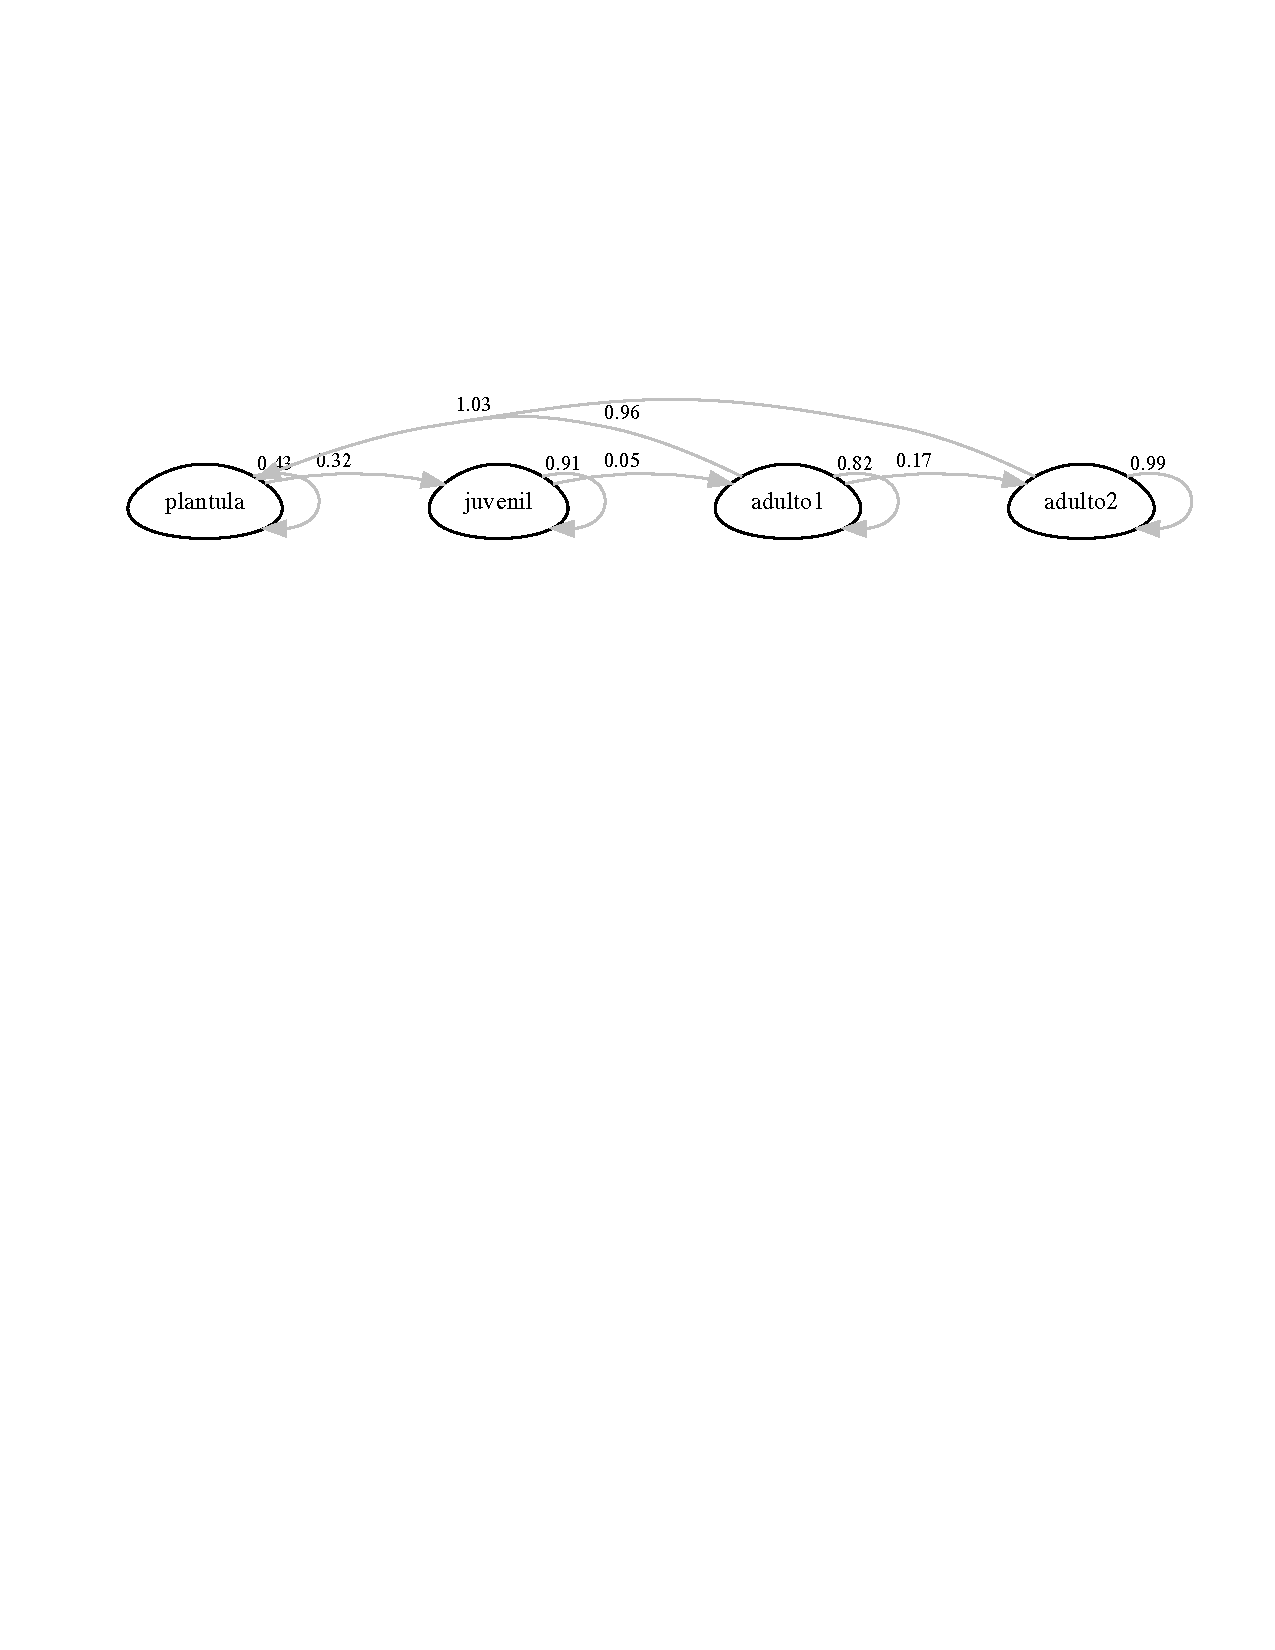
\includegraphics[keepaspectratio]{109-Crecimiento_poblacional_files/figure-pdf/cre_pop_1-1.pdf}}

Segunda matriz

\begin{Shaded}
\begin{Highlighting}[]
\CommentTok{\#Matriz de la poblacion 1, año 2}
\NormalTok{mat1}\FloatTok{.2} \OtherTok{\textless{}{-}} \FunctionTok{matrix}\NormalTok{ (}\FunctionTok{c}\NormalTok{(}\FloatTok{0.43}\NormalTok{, }\FloatTok{0.00}\NormalTok{,  }\FloatTok{0.85}\NormalTok{,  }\FloatTok{3.38}\NormalTok{,}
                    \FloatTok{0.32}\NormalTok{, }\FloatTok{0.90}\NormalTok{,  }\FloatTok{0.00}\NormalTok{,  }\FloatTok{0.00}\NormalTok{, }
                    \FloatTok{0.00}\NormalTok{, }\FloatTok{0.02}\NormalTok{,  }\FloatTok{0.77}\NormalTok{,  }\FloatTok{0.11}\NormalTok{,}
                    \FloatTok{0.00}\NormalTok{, }\FloatTok{0.00}\NormalTok{,  }\FloatTok{0.19}\NormalTok{,  }\FloatTok{0.88}\NormalTok{), }
          \AttributeTok{nrow =} \DecValTok{4}\NormalTok{, }\AttributeTok{ncol=}\DecValTok{4}\NormalTok{, }\AttributeTok{byrow =} \ConstantTok{TRUE}\NormalTok{, }
          \AttributeTok{dimnames =} \FunctionTok{list}\NormalTok{(estadios, estadios))}

\FunctionTok{plot\_life\_cycle}\NormalTok{(mat1}\FloatTok{.2}\NormalTok{, }\AttributeTok{stages =}\NormalTok{ estadios, }\AttributeTok{fontsize =} \DecValTok{10}\NormalTok{)}
\end{Highlighting}
\end{Shaded}

\pandocbounded{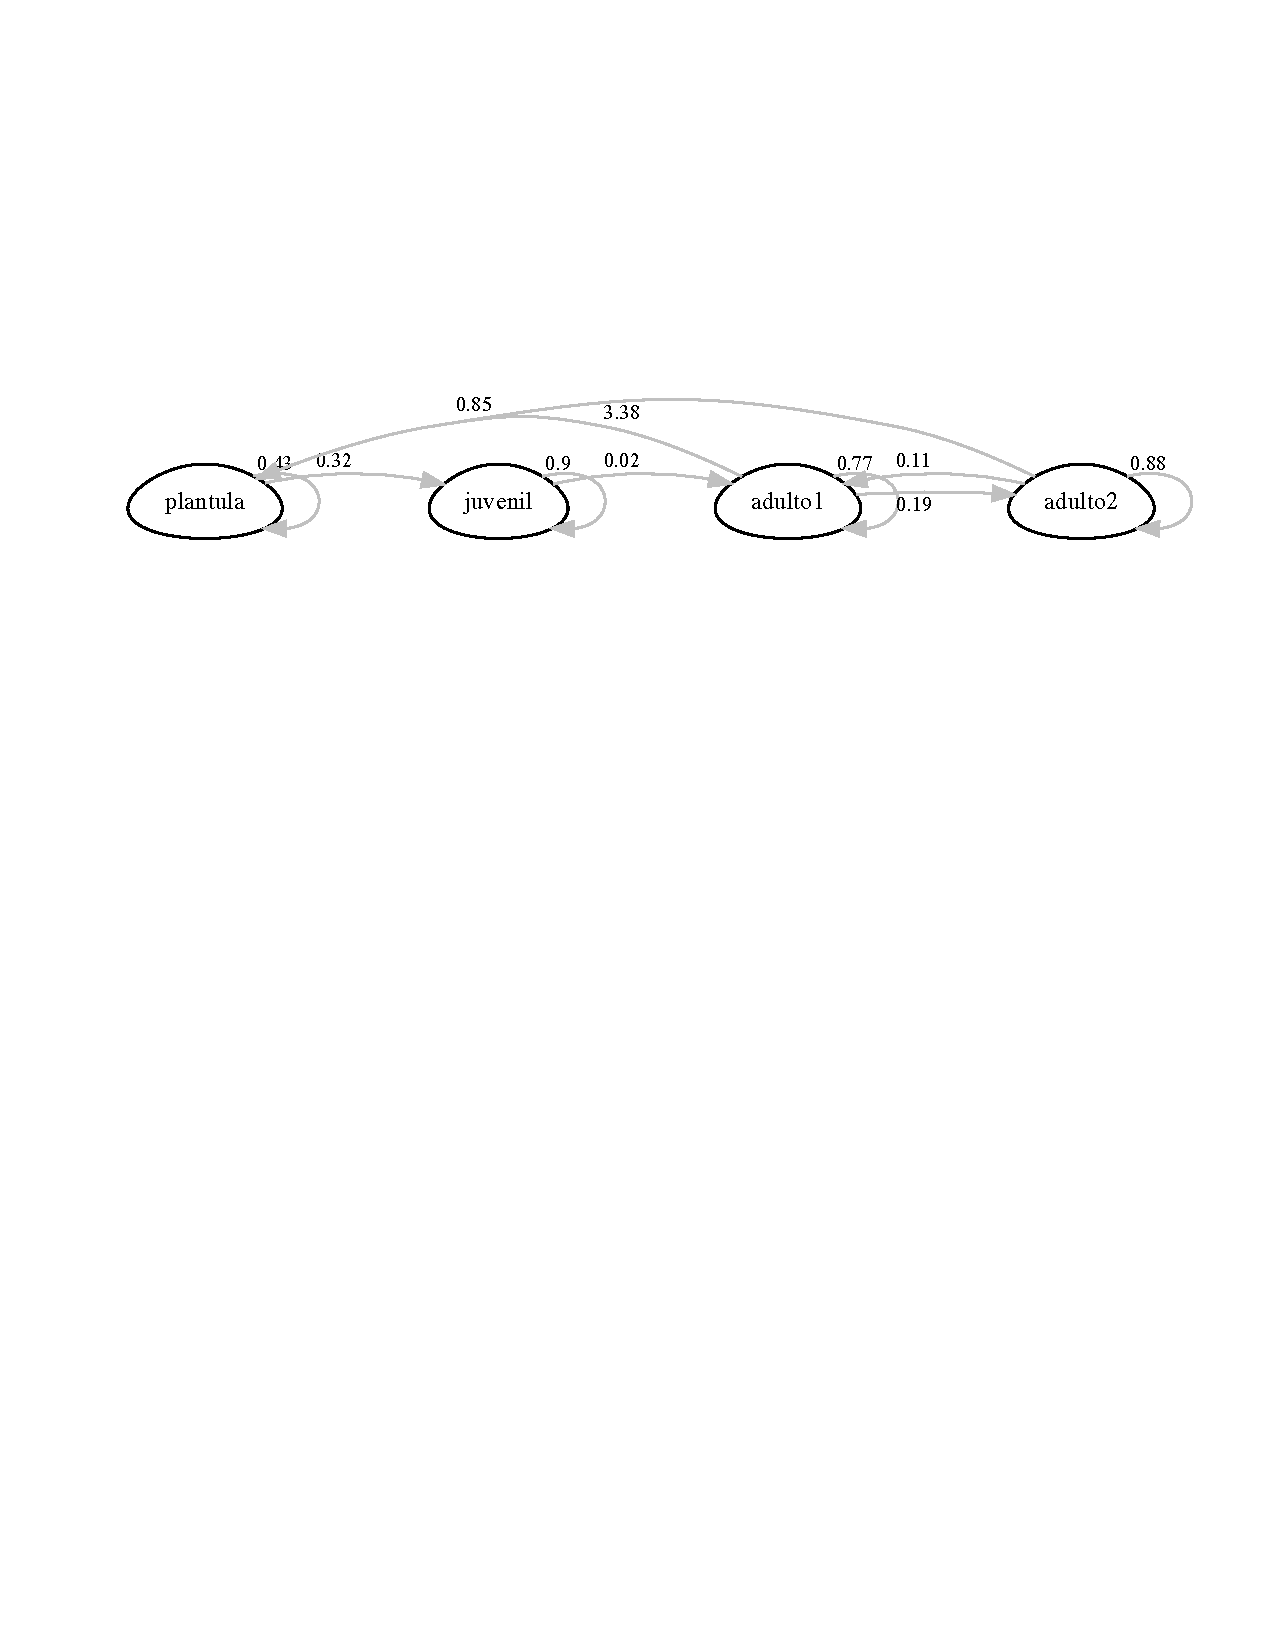
\includegraphics[keepaspectratio]{109-Crecimiento_poblacional_files/figure-pdf/cre_pop_1b-1.pdf}}

\begin{center}\rule{0.5\linewidth}{0.5pt}\end{center}

\section{\texorpdfstring{Calcular \(\lambda\) de la
población}{Calcular \textbackslash lambda de la población}}\label{calcular-lambda-de-la-poblaciuxf3n}

Calcular el \(\lambda\) de la población para los años 1 y 2,
respectivamente usando la función \texttt{eigen.analysis()} en
\texttt{popbio}.

En el primer año se observa que la población tiene un valor de
\(\lambda = 1.108\), lo que indica que la población crecería a largo
plazo aproximadamente un 11\%. En el segundo año, la población también
crece (8\%) al tener \(\lambda\) un valor de 1.084; aunque al ser menor
al del primer año, se indica que la tasa de crecimiento poblacional
disminuyó de un año a otro.

\begin{Shaded}
\begin{Highlighting}[]
\FunctionTok{options}\NormalTok{(}\AttributeTok{digits =} \DecValTok{5}\NormalTok{) }\CommentTok{\# Ajusta el número de decimales a mostrar}
\DocumentationTok{\#\#Calcula la lambda asintótica de cada población y año}
\NormalTok{eig1}\FloatTok{.1} \OtherTok{\textless{}{-}} \FunctionTok{eigen.analysis}\NormalTok{(mat1}\FloatTok{.1}\NormalTok{)}
\NormalTok{eig1}\FloatTok{.1}\SpecialCharTok{$}\NormalTok{lambda}
\end{Highlighting}
\end{Shaded}

\begin{verbatim}
[1] 1.1079
\end{verbatim}

\begin{Shaded}
\begin{Highlighting}[]
\NormalTok{eig1}\FloatTok{.2} \OtherTok{\textless{}{-}} \FunctionTok{eigen.analysis}\NormalTok{(mat1}\FloatTok{.2}\NormalTok{)}
\NormalTok{eig1}\FloatTok{.2}\SpecialCharTok{$}\NormalTok{lambda}
\end{Highlighting}
\end{Shaded}

\begin{verbatim}
[1] 1.0843
\end{verbatim}

\begin{Shaded}
\begin{Highlighting}[]
\NormalTok{t }\OtherTok{=} \FunctionTok{tribble}\NormalTok{(}\SpecialCharTok{\textasciitilde{}}\NormalTok{Año, }\SpecialCharTok{\textasciitilde{}}\NormalTok{lambda, }\StringTok{"Año 1"}\NormalTok{, eig1}\FloatTok{.1}\SpecialCharTok{$}\NormalTok{lambda, }\StringTok{"Año 2"}\NormalTok{, eig1}\FloatTok{.2}\SpecialCharTok{$}\NormalTok{lambda)}

\FunctionTok{flextable}\NormalTok{(t)}
\end{Highlighting}
\end{Shaded}

\global\setlength{\Oldarrayrulewidth}{\arrayrulewidth}

\global\setlength{\Oldtabcolsep}{\tabcolsep}

\setlength{\tabcolsep}{2pt}

\renewcommand*{\arraystretch}{1.5}



\providecommand{\ascline}[3]{\noalign{\global\arrayrulewidth #1}\arrayrulecolor[HTML]{#2}\cline{#3}}

\begin{longtable*}[c]{cc}



\ascline{1.5pt}{666666}{1-2}

\multicolumn{1}{>{}l}{\textcolor[HTML]{000000}{\fontsize{11}{11}\selectfont{Año}}} & \multicolumn{1}{>{}r}{\textcolor[HTML]{000000}{\fontsize{11}{11}\selectfont{lambda}}} \\

\ascline{1.5pt}{666666}{1-2}\endfirsthead 

\ascline{1.5pt}{666666}{1-2}

\multicolumn{1}{>{}l}{\textcolor[HTML]{000000}{\fontsize{11}{11}\selectfont{Año}}} & \multicolumn{1}{>{}r}{\textcolor[HTML]{000000}{\fontsize{11}{11}\selectfont{lambda}}} \\

\ascline{1.5pt}{666666}{1-2}\endhead



\multicolumn{1}{>{}l}{\textcolor[HTML]{000000}{\fontsize{11}{11}\selectfont{Año\ 1}}} & \multicolumn{1}{>{}r}{\textcolor[HTML]{000000}{\fontsize{11}{11}\selectfont{1.1079}}} \\





\multicolumn{1}{>{}l}{\textcolor[HTML]{000000}{\fontsize{11}{11}\selectfont{Año\ 2}}} & \multicolumn{1}{>{}r}{\textcolor[HTML]{000000}{\fontsize{11}{11}\selectfont{1.0843}}} \\

\ascline{1.5pt}{666666}{1-2}



\end{longtable*}



\arrayrulecolor[HTML]{000000}

\global\setlength{\arrayrulewidth}{\Oldarrayrulewidth}

\global\setlength{\tabcolsep}{\Oldtabcolsep}

\renewcommand*{\arraystretch}{1}

La tasa de crecimiento asintótica representa la tasa a la que crecería
una población a largo plazo, si no cambiaran las condiciones bajo las
cuales se construyó el modelo. Es decir, si no cambiaran en el tiempo
las condiciones bióticas, abióticas y de manejo que influyen en las
tasas vitales (i.e.~tasas de crecimiento, supervivencia y reproducción)
de dicha población. Por supuesto, nosotros sabemos que no es posible una
consistencia en todas las tasas vitales a largo plazo, siempre ocurren
cambios temporales determinístico o estocástico. Por ejemplo, la
ausencia de mortalidad de adultos durante los dos periodos de monitoreo
en nuestro caso. Es seguro que esta condición existe en campo, pero
nuestra muestra no lo captó, lo que llevó a reducir el valor de
supervivencia en una pequeña fracción -que supone una pérdida de
individuos y un valor de permanencia en la categoría menor de 1.0, cuyo
efecto es mínimo sobre el crecimiento poblacional. Este tipo de ajuste
en las entradas de la matriz lleva a remarcar que es importante que el
valor de \(\lambda\) nunca se use en sentido estricto.

También es fundamental tomar en cuenta que, \(\lambda\) no es la tasa a
la que se espera que la población creciera en el corto plazo. De hecho,
una población con \(\lambda\) \textless1 pudiera crecer en el corto
plazo, antes de declinar en el largo plazo y \(vice-versa\). Asimismo,
cabe señalar que la tasa de crecimiento poblacional de corto plazo es
calculada usando los índices de la dinámica transitoria (ver el capítulo
de \href{112-Dinamica_de_Transiciones.qmd}{Dinámica de transiciones}).

\begin{tcolorbox}[enhanced jigsaw, arc=.35mm, bottomrule=.15mm, bottomtitle=1mm, breakable, colback=white, colbacktitle=quarto-callout-warning-color!10!white, colframe=quarto-callout-warning-color-frame, coltitle=black, left=2mm, leftrule=.75mm, opacityback=0, opacitybacktitle=0.6, rightrule=.15mm, title=\textcolor{quarto-callout-warning-color}{\faExclamationTriangle}\hspace{0.5em}{Advertencia}, titlerule=0mm, toprule=.15mm, toptitle=1mm]

\textbf{λ describe el presente, no predice el futuro.} Aunque el
lenguaje natural sugiere que ``λ = 1.10 quiere decir que la población
crecerá un 10\% por año'', esto sólo se cumpliría si las tasas vitales
fueran exactamente las mismas todos los años --- algo prácticamente
nunca cierto. λ es una \textbf{descripción comparable} del estado
demográfico actual de la población (Crone et al.~2013), útil para
comparar entre sitios, periodos o tratamientos. Para predicciones a
corto plazo conviene usar análisis de dinámica transitoria; para
escenarios variables, la tasa estocástica \(\lambda_e\) (sección
siguiente).

\end{tcolorbox}

Los meta-análisis (Crone et al.~2013), en cambio, han demostrado que
\(\lambda\) es una medida robusta de las condiciones actuales, ya que
ésta explica la dinámica de las poblaciones durante el período de tiempo
en el que se parametrizaron los modelos. Asimismo, \(\lambda\) es una
buena medida del estado de la población, por lo que es una forma
apropiada de comparar el comportamiento de las poblaciones bajo
diferentes condiciones, incluyendo variación abiótica, biótica y de
manejo. Por ejemplo, los valores de \(\lambda\) permiten comparar el
comportamiento de una población en distintos periodos de tiempo y con
ello entender cómo la variación en las condiciones climáticas afecta su
dinámica. Las comparaciones también pueden ser entre poblaciones de la
misma especie distribuidas en distintos sitios, para entender los
efectos de la variación en el manejo, la vegetación u otras diferencias
entre sitios (vea el capítulo ``Variación temporal y espacial por
simulaciones'')

\begin{center}\rule{0.5\linewidth}{0.5pt}\end{center}

\section{Calcular el incremento de crecimiento poblacional por
año}\label{calcular-el-incremento-de-crecimiento-poblacional-por-auxf1o}

En esta sección demostramos el crecimiento esperado por año, usando la
función \texttt{pop.projection()} en el paquete \texttt{popbio}. Esta
función requiere que se especifique la matriz de transición, la cantidad
de individuos en cada estado al inicio del estudio y el número de años a
proyectar. En nuestro caso, proyectamos 7 años.

El resultado es una lista de los siguientes parámetros:

\begin{itemize}
\tightlist
\item
  El valor de \(\lambda\) para el periodo proyectado (7 años)
\item
  La distribución estable de la población
\item
  El número de individuos esperado en cada etapa y año proyectado
\item
  El tamaño poblacional esperado para cada año proyectado (suma de
  individuos en cada estadio)
\item
  El crecimiento intrínseco esperado para cada año proyectado, entendido
  como tasa de crecimiento potencial máxima de una población en
  condiciones ambientales ideales (Skalski, Ryding \& Millspaugh, 2010).
\end{itemize}

A partir de una población inicial de 10 individuos en cada estadio (25\%
del total de la población en cada uno) y después de proyectar la
población por siete iteraciones, podemos ver que el valor de \(\lambda\)
esperado es muy similar al calculado anteriormente, ±12\% de
crecimiento. Las diferencias radican en el vector de estadios, en el
cual se observan cambios importantes en la proporción de individuos por
estadio. La proporción de juveniles y plántulas, de ser un 25 \%
respectivamente, incrementa drásticamente y pasa a dominar la población
(90 \%, suma de ambas) en seis años. El crecimiento poblacional se mide
con la suma de los individuos en cada estadio por año proyectado
(\textbf{pop.sizes}) sobre la cantidad de individuos del año anterior.
Por ejemplo, en el primer año la población pasa de 40 individuos a 56.8
individuos, lo que evidencia un incremento en la abundancia de
individuos, correspondiente a un crecimiento de 42\% (56.8/40=1.42). En
el segundo año se espera que la población crezca de 56.8 a 70.2
individuos, lo que representa un crecimiento de 24\% (70.2/56.8=1.24).

\section{Proyección de la población 1, año
1}\label{proyecciuxf3n-de-la-poblaciuxf3n-1-auxf1o-1}

\begin{Shaded}
\begin{Highlighting}[]
\NormalTok{pop\_1 }\OtherTok{\textless{}{-}} \FunctionTok{pop.projection}\NormalTok{(mat1}\FloatTok{.1}\NormalTok{, }\AttributeTok{n =} \FunctionTok{c}\NormalTok{(}\DecValTok{10}\NormalTok{, }\DecValTok{10}\NormalTok{, }\DecValTok{10}\NormalTok{, }\DecValTok{10}\NormalTok{), }\AttributeTok{iterations =} \DecValTok{7}\NormalTok{)}
\NormalTok{pop\_1}
\end{Highlighting}
\end{Shaded}

\begin{verbatim}
$lambda
[1] 1.1176

$stable.stage
plantula  juvenil  adulto1  adulto2 
 0.33904  0.43907  0.07284  0.14904 

$stage.vectors
          0    1      2      3       4       5       6
plantula 10 24.2 30.503 33.542 35.5279 37.4740 39.8193
juvenil  10 12.3 18.937 26.994 35.2977 43.4899 51.5674
adulto1  10  8.7  7.749  7.301  7.3365  7.7808  8.5548
adulto2  10 11.6 12.963 14.151 15.2504 16.3451 17.5044

$pop.sizes
[1]  40.000  56.800  70.152  81.988  93.413 105.090 117.446

$pop.changes
[1] 1.4200 1.2351 1.1687 1.1393 1.1250 1.1176
\end{verbatim}

\subsubsection{Visualizar el crecimiento poblacional proyectado por
año}\label{visualizar-el-crecimiento-poblacional-proyectado-por-auxf1o}

El crecimiento poblacional proyectado por año se puede visualizar,
usando la función \textbf{plot} en el paquete \texttt{popbio}. En este
caso, se observa que la población crece de forma exponencial, lo que es
consistente con el valor de \(\lambda\) calculado anteriormente. Este
mismo código puede ser usado para responder las siguientes preguntas:
¿Qué pasa si cambian el número de individuos en cada estadio inicial?
¿Qué pasa si cambian la cantidad de iteraciones/time a un número grande?
Para esto, se tiene que modificar \textbf{n} y el número 7, que
representa las iteraciones.

\begin{Shaded}
\begin{Highlighting}[]
\NormalTok{n }\OtherTok{=} \FunctionTok{c}\NormalTok{(}\DecValTok{10}\NormalTok{, }\DecValTok{10}\NormalTok{, }\DecValTok{10}\NormalTok{, }\DecValTok{10}\NormalTok{) }\CommentTok{\# Definir el número de individuos en cada estadio inicial}
\NormalTok{cambio }\OtherTok{=} \FunctionTok{pop.projection}\NormalTok{(mat1}\FloatTok{.1}\NormalTok{, n, }\DecValTok{7}\NormalTok{)}

\FunctionTok{plot}\NormalTok{(}
\NormalTok{  cambio}\SpecialCharTok{$}\NormalTok{pop.size,}
  \AttributeTok{type =} \StringTok{"b"}\NormalTok{,}
  \AttributeTok{xlab =} \StringTok{"Año"}\NormalTok{,}
  \AttributeTok{ylab =} \StringTok{"Tamaño poblacional"}\NormalTok{,}
  \AttributeTok{main =} \StringTok{"Proyección de la población 1, año 1"}
\NormalTok{)}
\end{Highlighting}
\end{Shaded}

\pandocbounded{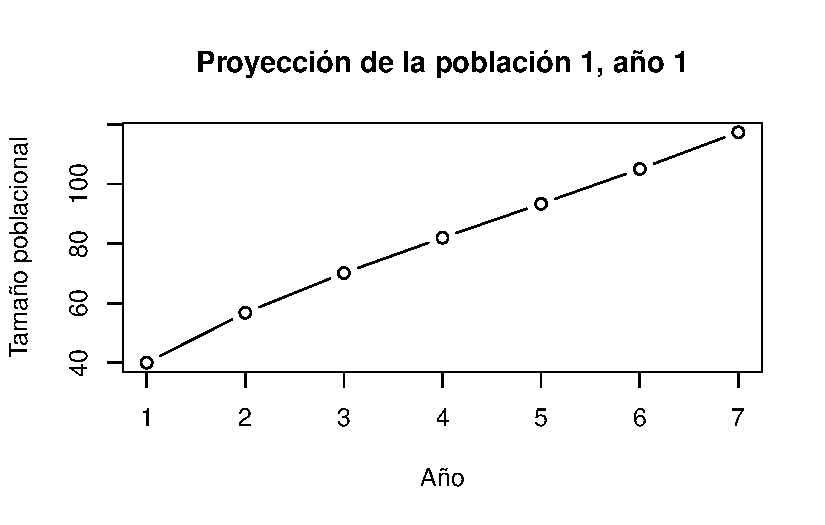
\includegraphics[keepaspectratio]{109-Crecimiento_poblacional_files/figure-pdf/unnamed-chunk-3-1.pdf}}

\subsection{Cambio porcentual de individuos por estadio en cada año
proyectado}\label{cambio-porcentual-de-individuos-por-estadio-en-cada-auxf1o-proyectado}

La proporción esperada de individuos en cada estadio por año proyectado
se puede gráficar usando la función \texttt{stage.vector.plot()} en el
paquete \texttt{popbio}. En este caso, se ve el cambio proporcional de
cada estadio a lo largo de 6 años que la población proyectada es
dominada por plántulas y juveniles, lo que es consistente con los
valores de \textbf{cambio\$pop.size} calculados anteriormente.

\begin{Shaded}
\begin{Highlighting}[]
\NormalTok{n }\OtherTok{=} \FunctionTok{c}\NormalTok{(}\DecValTok{10}\NormalTok{, }\DecValTok{10}\NormalTok{, }\DecValTok{10}\NormalTok{, }\DecValTok{10}\NormalTok{) }\CommentTok{\# Definir el número de individuos en cada estadio inicial}
\NormalTok{cambio }\OtherTok{=} \FunctionTok{pop.projection}\NormalTok{(mat1}\FloatTok{.1}\NormalTok{, n, }\DecValTok{7}\NormalTok{)}

\FunctionTok{stage.vector.plot}\NormalTok{(cambio}\SpecialCharTok{$}\NormalTok{stage.vectors, }\AttributeTok{col =} \DecValTok{2}\SpecialCharTok{:}\DecValTok{4}\NormalTok{, }\AttributeTok{ylim =} \FunctionTok{c}\NormalTok{(}\DecValTok{0}\NormalTok{, }\FloatTok{0.6}\NormalTok{))}
\end{Highlighting}
\end{Shaded}

\pandocbounded{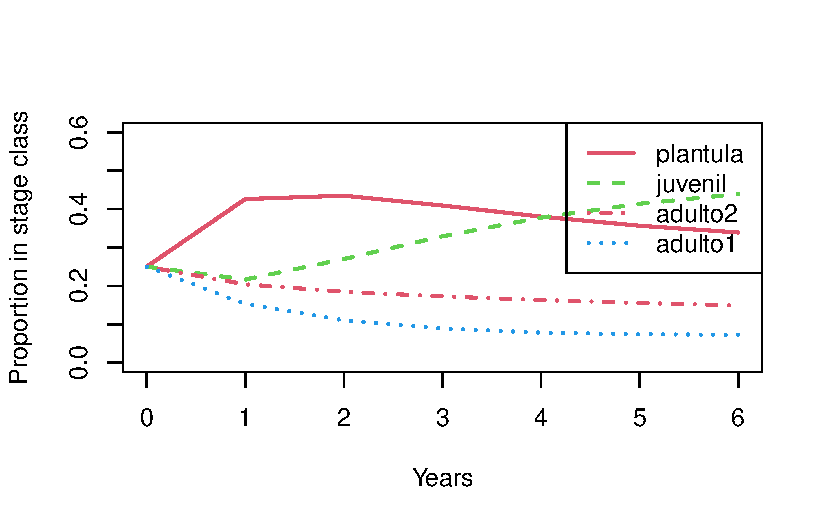
\includegraphics[keepaspectratio]{109-Crecimiento_poblacional_files/figure-pdf/unnamed-chunk-4-1.pdf}}

\section{\texorpdfstring{Comparación de valor de \(\lambda\) entre
poblaciones (1 y
2)}{Comparación de valor de \textbackslash lambda entre poblaciones (1 y 2)}}\label{comparaciuxf3n-de-valor-de-lambda-entre-poblaciones-1-y-2}

Nuestra segunda población de \emph{Laelia speciosa} se establece en un
hábitat similar a la población 1 y fue monitoreada durante al mismo
tiempo. Sin embargo, ésta fue sujeta a la extracción. Si comparamos los
valores de \(\lambda\) de nuestras dos poblaciones, podemos hacer
inferencias sobre los efectos de la extracción. La población 2 no
produjo frutos y tampoco se observaron plántulas. Debido a esto, fue
necesario incluir el valor de 0.001 para la transición de la matriz
adulta2-\textgreater{} plántula y con esto asegurar que nuestra matriz
de estudio sea irreducible y primitiva (ver el capítulo de
\href{110-Propriedades.qmd}{Propiedades poblacionales}).

\section{Proyección de la población 2, año
1}\label{proyecciuxf3n-de-la-poblaciuxf3n-2-auxf1o-1}

\begin{Shaded}
\begin{Highlighting}[]
\CommentTok{\#Matriz de la población 2, año 1}
\NormalTok{mat2}\FloatTok{.1} \OtherTok{\textless{}{-}} \FunctionTok{matrix}\NormalTok{ (}\FunctionTok{c}\NormalTok{(}\FloatTok{0.50}\NormalTok{, }\FloatTok{0.00}\NormalTok{, }\FloatTok{0.00}\NormalTok{, }\FloatTok{0.001}\NormalTok{,}
                    \FloatTok{0.16}\NormalTok{, }\FloatTok{0.79}\NormalTok{, }\FloatTok{0.00}\NormalTok{, }\FloatTok{0.00}\NormalTok{, }
                    \FloatTok{0.00}\NormalTok{, }\FloatTok{0.12}\NormalTok{, }\FloatTok{0.78}\NormalTok{, }\FloatTok{0.11}\NormalTok{,}
                    \FloatTok{0.00}\NormalTok{, }\FloatTok{0.00}\NormalTok{, }\FloatTok{0.21}\NormalTok{, }\FloatTok{0.88}\NormalTok{), }
          \AttributeTok{nrow =} \DecValTok{4}\NormalTok{, }\AttributeTok{ncol=}\DecValTok{4}\NormalTok{, }\AttributeTok{byrow =} \ConstantTok{TRUE}\NormalTok{,}
          \AttributeTok{dimnames =} \FunctionTok{list}\NormalTok{(estadios, estadios))}

\NormalTok{mat2}\FloatTok{.1}
\end{Highlighting}
\end{Shaded}

\begin{verbatim}
         plantula juvenil adulto1 adulto2
plantula     0.50    0.00    0.00   0.001
juvenil      0.16    0.79    0.00   0.000
adulto1      0.00    0.12    0.78   0.110
adulto2      0.00    0.00    0.21   0.880
\end{verbatim}

\begin{Shaded}
\begin{Highlighting}[]
\NormalTok{eig2}\FloatTok{.1} \OtherTok{\textless{}{-}} \FunctionTok{eigen.analysis}\NormalTok{(mat2}\FloatTok{.1}\NormalTok{)}
\NormalTok{eig2}\FloatTok{.1}\SpecialCharTok{$}\NormalTok{lambda}
\end{Highlighting}
\end{Shaded}

\begin{verbatim}
[1] 0.99013
\end{verbatim}

La población bajo extracción tiene un valor de \(\lambda\) menor (0.990)
a aquella en que no se observa esta actividad de manejo. Sin embargo,
debemos ser cautelosos con nuestra interpretación sobre los efectos de
la extracción, debido a que cualquier diferencia relacionada con la
extracción está mezclada o enmascarada con las diferencias entre los dos
sitios. Para lograr una comparación robusta, se debe llevar a cabo un
experimento de extracción en el mismo sitio o tener varios sitios de
extracción y también varios sitios sin extracción.

\begin{tcolorbox}[enhanced jigsaw, arc=.35mm, bottomrule=.15mm, bottomtitle=1mm, breakable, colback=white, colbacktitle=quarto-callout-warning-color!10!white, colframe=quarto-callout-warning-color-frame, coltitle=black, left=2mm, leftrule=.75mm, opacityback=0, opacitybacktitle=0.6, rightrule=.15mm, title=\textcolor{quarto-callout-warning-color}{\faExclamationTriangle}\hspace{0.5em}{Advertencia}, titlerule=0mm, toprule=.15mm, toptitle=1mm]

\textbf{Una diferencia entre dos poblaciones no atribuye causa.} En este
ejemplo, la población 2 (con extracción) tiene \(\lambda = 0.99\) y la
población 1 (sin extracción) \(\lambda = 1.11\). La diferencia es
consistente con un efecto de la extracción, \textbf{pero no lo
demuestra}: cualquier diferencia ambiental, microclimática o histórica
entre los dos sitios podría explicar parte o toda la diferencia. Para
inferir causa hace falta replicación: varios sitios con extracción y
varios sitios control en la misma región, idealmente con datos previos
al inicio del manejo.

\end{tcolorbox}

\begin{center}\rule{0.5\linewidth}{0.5pt}\end{center}

\section{\texorpdfstring{Intervalos de confianza de
\(\lambda\)}{Intervalos de confianza de \textbackslash lambda}}\label{intervalos-de-confianza-de-lambda}

\begin{tcolorbox}[enhanced jigsaw, arc=.35mm, bottomrule=.15mm, bottomtitle=1mm, breakable, colback=white, colbacktitle=quarto-callout-note-color!10!white, colframe=quarto-callout-note-color-frame, coltitle=black, left=2mm, leftrule=.75mm, opacityback=0, opacitybacktitle=0.6, rightrule=.15mm, title=\textcolor{quarto-callout-note-color}{\faInfo}\hspace{0.5em}{Nota}, titlerule=0mm, toprule=.15mm, toptitle=1mm]

\textbf{Dos enfoques para los intervalos de incertidumbre de λ.}

\begin{itemize}
\tightlist
\item
  \textbf{Bootstrap (\texttt{popbio::boot.transitions()}):} remuestrea
  con reemplazo los individuos observados y vuelve a calcular λ.
  Apropiado cuando el tamaño de muestra es razonable y todas las
  transiciones tienen al menos algunas observaciones.
\item
  \textbf{Dirichlet bayesiano (\texttt{raretrans}):} usa la distribución
  posterior de las transiciones, derivada de una previa Dirichlet.
  Apropiado cuando el tamaño de muestra es pequeño o cuando hay
  transiciones raras observadas con frecuencia 0/n.~Ver el capítulo de
  \hyperref[acercamiento-bayesiano-para-calcular-transiciones-y-fecundidades]{Acercamiento
  bayesiano}.
\end{itemize}

\end{tcolorbox}

Para interpretar \(\lambda\) apropiadamente necesitamos calcular los
intervalos de confianza (IC). Estos intervalos pueden ser calculados con
un método de remuestreo con reemplazo (i.e.~bootstrap), utilizando las
transiciones de estado de los individuos de un periodo a otro; es decir,
los datos (i.e.~\(stage-fate\)) usados para construir la matriz de
transiciones (ver el capítulo de \hyperref[MatricesT]{Transiciones}). En
el remuestreo se puede especificar el tamaño de la muestra remuestreada,
la cual fue de 1000 en nuestro caso. Cabe señalar que se tendrán
intervalos de confianza amplios cuando se tiene una muestra pequeña de
datos originales, o si se tienen pocas observaciones de aquellas
transiciones que contribuyen en mayor medida a \(\lambda\).
Adicionalmente, se puede usar el método del paquete \texttt{raretrans}
(ver el capítulo de
\hyperref[acercamiento-bayesiano-para-calcular-transiciones-y-fecundidades]{Acercamiento
bayesiano}), que es apropiado para tamaños de muestra pequeños. La
diferencia entre los dos métodos es que \texttt{popbio} selecciona
aleatoriamente la cantidad de individuos en cada estadio (bootstrap),
mientras que \texttt{raretrans} simula a partir de la distribución
posterior Dirichlet.

En el presente caso, calculamos los intervalos de confianza de
\(\lambda\) para la población 1, correspondientes al año 1 y 2. En ambos
años, los intervalos son amplios.

Usando la función \texttt{boot.transitions()} del paquete
\texttt{popbio}, se pueden calcular los intervalos de confianza de
\(\lambda\). Esta función requiere que se especifiquen los estadios de
la matriz y el número de remuestreos. En nuestro caso, usamos 1000
remuestreos y especificamos los estadios como ``pl'', ``j'', ``a1'' y
``a2''.

\begin{itemize}
\item
  \textbf{boot.transitions(transitions, iterations, sort = stages)}
\item
  transitions: un data frame con las transiciones de los individuos de
  un periodo a otro (i.e.~\(stage-fate\)).
\item
  iterations: el número de remuestreos a realizar.
\item
  sort: un vector con los nombres de los estadios en el orden en que se
  encuentran en la matriz de transición.
\end{itemize}

\begin{Shaded}
\begin{Highlighting}[]
\CommentTok{\#Intervalos de confianza (IC) de λ para la población 1, año 1}
\CommentTok{\#Indica el directorio de trabajo y definir los estadios}

\NormalTok{laelia1 }\OtherTok{\textless{}{-}} \FunctionTok{read.table}\NormalTok{(}\StringTok{"data/laelia1.txt"}\NormalTok{, }\AttributeTok{header =} \ConstantTok{TRUE}\NormalTok{) }\CommentTok{\# subir los datos de la población 1, año 1}

\NormalTok{pop1}\FloatTok{.1} \OtherTok{=}\NormalTok{ laelia1 }\CommentTok{\# renombrar el data frame para facilitar su uso}

\NormalTok{stages }\OtherTok{\textless{}{-}} \FunctionTok{c}\NormalTok{(}\StringTok{"pl"}\NormalTok{, }\StringTok{"j"}\NormalTok{, }\StringTok{"a1"}\NormalTok{, }\StringTok{"a2"}\NormalTok{) }\CommentTok{\# identificación de los estadios}

\NormalTok{n }\OtherTok{\textless{}{-}} \FunctionTok{nrow}\NormalTok{(pop1}\FloatTok{.1}\NormalTok{) }\CommentTok{\# Crear una variable n que contiene el número de filas del data.frame}

\NormalTok{x }\OtherTok{\textless{}{-}} \FunctionTok{boot.transitions}\NormalTok{(pop1}\FloatTok{.1}\NormalTok{, }\DecValTok{1000}\NormalTok{, }\AttributeTok{sort =}\NormalTok{ stages) }\CommentTok{\# la boot.transition selecciona al azar la cantidad de individuos en cada estadios: función esta en el paquete "popbio"}

\NormalTok{ic1 }\OtherTok{\textless{}{-}} \FunctionTok{quantile}\NormalTok{(x}\SpecialCharTok{$}\NormalTok{lambda, }\FunctionTok{c}\NormalTok{(}\FloatTok{0.025}\NormalTok{, }\FloatTok{0.975}\NormalTok{))}
\NormalTok{ic1}
\end{Highlighting}
\end{Shaded}

\begin{verbatim}
  2.5%  97.5% 
1.0000 1.2168 
\end{verbatim}

\begin{Shaded}
\begin{Highlighting}[]
\CommentTok{\#IC para la población 1, año 2}
\end{Highlighting}
\end{Shaded}

\subsection{Simulación de las transiciones de la población 1, año
2}\label{simulaciuxf3n-de-las-transiciones-de-la-poblaciuxf3n-1-auxf1o-2}

\begin{Shaded}
\begin{Highlighting}[]
\NormalTok{laelia2 }\OtherTok{\textless{}{-}} \FunctionTok{read.table}\NormalTok{(}\StringTok{"data/laelia2.txt"}\NormalTok{, }\AttributeTok{header =} \ConstantTok{TRUE}\NormalTok{)}

\NormalTok{pop1}\FloatTok{.2} \OtherTok{=}\NormalTok{ laelia2}

\NormalTok{stages }\OtherTok{\textless{}{-}} \FunctionTok{c}\NormalTok{(}\StringTok{"pl"}\NormalTok{, }\StringTok{"j"}\NormalTok{, }\StringTok{"a1"}\NormalTok{, }\StringTok{"a2"}\NormalTok{)}

\NormalTok{n }\OtherTok{\textless{}{-}} \FunctionTok{nrow}\NormalTok{(pop1}\FloatTok{.2}\NormalTok{)}
\NormalTok{x2 }\OtherTok{\textless{}{-}} \FunctionTok{boot.transitions}\NormalTok{(pop1}\FloatTok{.2}\NormalTok{, }\DecValTok{1000}\NormalTok{, }\AttributeTok{sort =}\NormalTok{ stages)}
\NormalTok{ic2 }\OtherTok{\textless{}{-}} \FunctionTok{quantile}\NormalTok{(x2}\SpecialCharTok{$}\NormalTok{lambda, }\FunctionTok{c}\NormalTok{(}\FloatTok{0.025}\NormalTok{, }\FloatTok{0.975}\NormalTok{))}
\NormalTok{ic2}
\end{Highlighting}
\end{Shaded}

\begin{verbatim}
   2.5%   97.5% 
0.96918 1.19530 
\end{verbatim}

\begin{Shaded}
\begin{Highlighting}[]
\CommentTok{\#Nota:  Los datos de algunas transiciones especificas no siempre se obtienen de los censos poblacionales, por lo que éstos pueden provenir de otros experimentos. Por ejemplo, si las observaciones de campo fueran nulas o escasas para la transición de semilla a plántula, éste dato se puede obtener de la literatura consultada o de experimentos previos o usar el método descrito en el capítulo de [Acercamiento bayesiano para calcular transiciones y fecundidades](108{-}Bayesian\_PPM.qmd). En estos casos se incorporaron las transiciones a la matriz de la siguiente forma al estimar el IC: }

\CommentTok{\# pl.pl\textless{}{-}0.7 \#a la permanencia en plantula se le asigno el valor 0.7 }
\CommentTok{\# pl.j\textless{}{-}0.1 \#a la transicion plantula{-}juvenil se le asignó el valor 0.1}
\CommentTok{\# x\textless{}{-}boot.transitions(pop1, 1000, add = c(1,1, pl.pl, 2,1, pl.j), sort=stages)}
\end{Highlighting}
\end{Shaded}

Note que para la población en el primer año el intervalo de confianza de
\(\lambda\) es de 1.00 a 1.21, lo que indica que el mejor estimado de la
tasa de crecimiento poblacional esperada está entre 0\% y 21\%. En el
segundo año, el intervalo de confianza es de 0.97 a 1.19, lo que indica
que la tasa de crecimiento poblacional pudiese ser entre una reducción
de ±3\% a aumento de 19\%.

\begin{Shaded}
\begin{Highlighting}[]
\FunctionTok{bind\_rows}\NormalTok{(ic1, ic2) }\SpecialCharTok{\%\textgreater{}\%}
  \FunctionTok{mutate}\NormalTok{(}\AttributeTok{year =} \FunctionTok{c}\NormalTok{(}\StringTok{"año 1"}\NormalTok{, }\StringTok{"año 2"}\NormalTok{)) }\SpecialCharTok{\%\textgreater{}\%}
  \FunctionTok{select}\NormalTok{(year, }\FunctionTok{everything}\NormalTok{()) }\SpecialCharTok{\%\textgreater{}\%}
  \FunctionTok{rename}\NormalTok{(}\StringTok{"IC 2.5\%"} \OtherTok{=} \StringTok{\textasciigrave{}}\AttributeTok{2.5\%}\StringTok{\textasciigrave{}}\NormalTok{, }\StringTok{"IC 97.5\%"} \OtherTok{=} \StringTok{\textasciigrave{}}\AttributeTok{97.5\%}\StringTok{\textasciigrave{}}\NormalTok{) }\SpecialCharTok{\%\textgreater{}\%}
\NormalTok{  knitr}\SpecialCharTok{::}\FunctionTok{kable}\NormalTok{(}\AttributeTok{digits =} \DecValTok{3}\NormalTok{, }\AttributeTok{caption =} \StringTok{"Intervalos de confianza de λ"}\NormalTok{)}
\end{Highlighting}
\end{Shaded}

\begin{longtable}[]{@{}lrr@{}}
\caption{Intervalos de confianza de λ}\tabularnewline
\toprule\noalign{}
year & IC 2.5\% & IC 97.5\% \\
\midrule\noalign{}
\endfirsthead
\toprule\noalign{}
year & IC 2.5\% & IC 97.5\% \\
\midrule\noalign{}
\endhead
\bottomrule\noalign{}
\endlastfoot
año 1 & 1.000 & 1.217 \\
año 2 & 0.969 & 1.195 \\
\end{longtable}

\begin{center}\rule{0.5\linewidth}{0.5pt}\end{center}

\section{Ambiente variable}\label{ambiente-variable}

En el ejemplo anterior, hemos asumido que las condiciones bajo las
cuales se construyeron las matrices de transición son constantes en el
tiempo. Sin embargo, sabemos que esto no es cierto, ya que las
condiciones bióticas y abióticas cambian con el tiempo y espacio. Por lo
tanto, \(\lambda\) no debe ser interpretado literalmente como un valor
específico, ni tampoco como una herramienta predictiva. En trabajos de
viabilidad de población uno de los objetivos es evaluar cómo la
variabilidad demográfica, biótica y abiótica impactan las tasas vitales
y por consecuencia el crecimiento afecta la dinámica poblacional. Para
ello, se puede calcular la tasa estocástica de crecimiento \(λ_e\) (ver
más adelante).

\section{\texorpdfstring{Tasa estocástica de crecimiento
\(λ_e\)}{Tasa estocástica de crecimiento λ\_e}}\label{tasa-estocuxe1stica-de-crecimiento-ux3bb_e}

La tasa estocástica de crecimiento o \(λ_e\) se puede estimar si se
cuenta con datos colectados por 2 o más periodos y, por lo tanto, se
tienen 2 o más matrices de transición. La tasa estocástica se puede
calcular a través del método de simulación de Cohen o por la
aproximación de Tuljapurkar (Caswell, 2001). En la simulación, las
matrices son seleccionadas aleatoriamente para un número específico de
intervalos de tiempo (50,000 por omisión en \texttt{popbio}). Se calcula
\(λ_e\) como la tasa media del crecimiento para un lapso de tiempo. En
la aproximación de Tuljapurkar, se calcula \(λ_e\) como el valor propio
dominante de la matriz de transición promedio. El método de Tuljapurkar
es más rápido, pero menos robusto que el método de simulación. Pero es
recomendable solamente cuando la variación entre las matrices de
diferentes periodos sean pequeñas (Caswell, 2001), aunque Morris y Doak
mencionan que el método funciona bastante bien aunque varían las
matrices (Morris \& Doak, 2002). En la próxima sección se muestra cómo
calcular \(λ_e\).

\begin{tcolorbox}[enhanced jigsaw, arc=.35mm, bottomrule=.15mm, bottomtitle=1mm, breakable, colback=white, colbacktitle=quarto-callout-note-color!10!white, colframe=quarto-callout-note-color-frame, coltitle=black, left=2mm, leftrule=.75mm, opacityback=0, opacitybacktitle=0.6, rightrule=.15mm, title=\textcolor{quarto-callout-note-color}{\faInfo}\hspace{0.5em}{Nota}, titlerule=0mm, toprule=.15mm, toptitle=1mm]

\textbf{¿Cuándo usar cada método para \(\lambda_e\)?}

\begin{itemize}
\tightlist
\item
  \textbf{Simulación de Cohen} (defecto en
  \texttt{popbio::stoch.growth.rate()}): selecciona aleatoriamente entre
  las matrices observadas durante miles de iteraciones y calcula la tasa
  media de crecimiento logarítmico. Más robusta, especialmente cuando
  las matrices difieren mucho entre sí.
\item
  \textbf{Aproximación de Tuljapurkar:} fórmula analítica basada en la
  matriz promedio y la covarianza entre entradas. Más rápida, pero
  precisa sólo cuando la variación entre matrices es modesta.
\end{itemize}

Cuando hay duda, reportar ambos: si difieren mucho, la variación entre
años es importante y la simulación es la métrica más confiable.

\end{tcolorbox}

Es apropiado tomar el tiempo de entender como se calcula \(λ_e\) y cómo
se interpreta. En primer lugar, la aproximación de Tuljapurkar se
calcula de la siguiente manera:

\[log(λ_e) = log(\bar\lambda_1)-\frac{1}{2}(\frac{\tau^2}{\bar\lambda_1^2})\],

donde \(\tau^2\) es igual a:

\[\tau^2=\sum_{i=1}^{S}\sum_{j=1}^{S}\sum_{k=1}^{S}\sum_{l=1}^{S}Cov(\alpha_{ij}, \alpha_{kl})\bar{S_{ij}}\bar{S_{kl}}\]

La variable de la ecuación incluye \(\bar\lambda_1\), que representa el
log del valor propio (\(λ\)) promedio de las matrices de transición
\(\bar{\text{A}}\), en el que cada entrada de la matriz es un valor
promedio de los elementos de las matrices analizadas. Si tenemos 4
matrices de transición, \(\bar{\text{A}}\) es la matriz de transición
promedio. Por ejemplo, si la transiciones de plántula a juvenil en la
matriz 1 es 0.1, en la matriz 2 es 0.2, en la matriz 3 es 0.15 y en la
matriz 4 es 0.05, entonces el valor promedio en la \(\bar{\text{A}}\) de
la transición de plántula a juvenil sería (0.1 + 0.2 + 0.15 + 0.05)/4 =
0.125. Por consecuencia el valor de \(\bar{\alpha}_{1,1}=0.125\) y así
sucesivamente para cada elemento de la matriz.

El componente \(\frac{\tau^2}{\bar\lambda_1^2}\) es un aproximado de la
variación temporal del crecimiento poblacional a causa de la
estocasticidad temporal. En este caso, \(\tau^2\) es el efecto de la
sensibilidad de \(\lambda\) causada por los cambios en los elementos
\(\bar{\alpha}_{i,j}\). La covarianza \(\text{Cov}\) mide las
correlaciones entre las transiciones de estado \(i\) a \(j\) y \(k\) a
\(l\), y se denota como \(Cov(\alpha_{ij}, \alpha_{kl})\). Recuerda que
no todos los valores en la matriz tienen el mismo impacto si fuesen a
cambiar (ver capítulo de elasticidad). Se espera que algunos de los
elementos tengan sobre \(\lambda\) un impacto relativo e influencia de
forma positiva o negativa, por lo que la covarianza puede ser positiva o
negativa. Por ejemplo, si la transición de plántula a juvenil aumenta,
es probable que la transición de juvenil a adulto aumente también en un
buen año, y viceversa; por lo tanto, la covarianza entre estas
transiciones es positiva. La covarianza tendrá un valor negativo, por
ejemplo, si aumenta la transición de plántulas a juvenil, lo cual
implicará una reducción en la cantidad de plántulas que siguen en este
estadio en el próximo año.

En lo anterior, una vez más, se asume que las condiciones bajo las
cuales se construyeron las matrices de transición son constantes en el
tiempo. Por lo tanto, \(λ_e\) no debe ser interpretado literalmente, ni
tampoco como una herramienta predictiva. En adición los valores de IC se
restan y se suma al valor de \(\lambda\) promedio obtenido para tener el
rango de 95\% de su valor.

\begin{Shaded}
\begin{Highlighting}[]
\NormalTok{matrices }\OtherTok{\textless{}{-}} \FunctionTok{list}\NormalTok{(mat1}\FloatTok{.1}\NormalTok{, mat1}\FloatTok{.2}\NormalTok{) }\CommentTok{\# Crear una lista de matrices de las poblaciones 1 de los 2 periodos de estudio}
\NormalTok{estocástico }\OtherTok{\textless{}{-}} \FunctionTok{stoch.growth.rate}\NormalTok{(matrices, }\AttributeTok{maxt =} \DecValTok{50000}\NormalTok{, }\AttributeTok{verbose =} \ConstantTok{FALSE}\NormalTok{) }\CommentTok{\# Selección aleatoria de matrices}
\CommentTok{\#estocástico}
\end{Highlighting}
\end{Shaded}

Se transforma tasa de base log y se obtiene \(λ_e\) por dos métodos
(Tuljapukar y simulación) y los IC por simulación

\begin{Shaded}
\begin{Highlighting}[]
\NormalTok{tuljapukar }\OtherTok{\textless{}{-}} \FunctionTok{exp}\NormalTok{(estocástico}\SpecialCharTok{$}\NormalTok{approx)}
\NormalTok{simulation }\OtherTok{\textless{}{-}} \FunctionTok{exp}\NormalTok{(estocástico}\SpecialCharTok{$}\NormalTok{sim)}

\CommentTok{\#tuljapukar \# λ  por Tuljapukar}
\CommentTok{\#simulation \# λ  por simulación}

\NormalTok{ic}\FloatTok{.1} \OtherTok{\textless{}{-}} \FunctionTok{exp}\NormalTok{(estocástico}\SpecialCharTok{$}\NormalTok{sim.CI[}\DecValTok{1}\NormalTok{])}
\NormalTok{ic}\FloatTok{.2} \OtherTok{\textless{}{-}} \FunctionTok{exp}\NormalTok{(estocástico}\SpecialCharTok{$}\NormalTok{sim.CI[}\DecValTok{2}\NormalTok{])}

\CommentTok{\#ic.1 \# El intervalo de confianza de λs por simulación inferior}
\CommentTok{\#ic.2 \# El intervalo de confianza de λs por simulación superior}
\end{Highlighting}
\end{Shaded}

\begin{Shaded}
\begin{Highlighting}[]
\NormalTok{Tul\_NA}\OtherTok{=}\ConstantTok{NA}

\FunctionTok{tribble}\NormalTok{(}\SpecialCharTok{\textasciitilde{}}\NormalTok{Método, }\SpecialCharTok{\textasciitilde{}}\NormalTok{λ, }\SpecialCharTok{\textasciitilde{}}\NormalTok{IC\_2}\FloatTok{.5}\NormalTok{, }\SpecialCharTok{\textasciitilde{}}\NormalTok{IC\_97}\FloatTok{.5}\NormalTok{,}
  \StringTok{"Tuljapukar"}\NormalTok{, tuljapukar, Tul\_NA, Tul\_NA,}
  \StringTok{"Simulación"}\NormalTok{, simulation, ic}\FloatTok{.1}\NormalTok{, ic}\FloatTok{.2}\NormalTok{) }\SpecialCharTok{\%\textgreater{}\%}
  \FunctionTok{flextable}\NormalTok{() }\SpecialCharTok{\%\textgreater{}\%}
  \FunctionTok{set\_header\_labels}\NormalTok{(Método }\OtherTok{=} \StringTok{"Método"}\NormalTok{, λ }\OtherTok{=} \StringTok{"λ\_e"}\NormalTok{, }\AttributeTok{IC\_2.5 =} \StringTok{"IC 2.5\%"}\NormalTok{, }\AttributeTok{IC\_97.5 =} \StringTok{"IC 97.5\%"}\NormalTok{) }\SpecialCharTok{\%\textgreater{}\%}
  \FunctionTok{set\_caption}\NormalTok{(}\AttributeTok{caption =} \StringTok{"Tasa estocástica de crecimiento λ\_e y IC"}\NormalTok{)}
\end{Highlighting}
\end{Shaded}

\global\setlength{\Oldarrayrulewidth}{\arrayrulewidth}

\global\setlength{\Oldtabcolsep}{\tabcolsep}

\setlength{\tabcolsep}{2pt}

\renewcommand*{\arraystretch}{1.5}



\providecommand{\ascline}[3]{\noalign{\global\arrayrulewidth #1}\arrayrulecolor[HTML]{#2}\cline{#3}}

\begin{longtable*}[c]{cccc}



\ascline{1.5pt}{666666}{1-4}

\multicolumn{1}{>{}l}{\textcolor[HTML]{000000}{\fontsize{11}{11}\selectfont{Método}}} & \multicolumn{1}{>{}r}{\textcolor[HTML]{000000}{\fontsize{11}{11}\selectfont{λ\_e}}} & \multicolumn{1}{>{}r}{\textcolor[HTML]{000000}{\fontsize{11}{11}\selectfont{IC\ 2.5\%}}} & \multicolumn{1}{>{}r}{\textcolor[HTML]{000000}{\fontsize{11}{11}\selectfont{IC\ 97.5\%}}} \\

\ascline{1.5pt}{666666}{1-4}\endfirsthead 

\ascline{1.5pt}{666666}{1-4}

\multicolumn{1}{>{}l}{\textcolor[HTML]{000000}{\fontsize{11}{11}\selectfont{Método}}} & \multicolumn{1}{>{}r}{\textcolor[HTML]{000000}{\fontsize{11}{11}\selectfont{λ\_e}}} & \multicolumn{1}{>{}r}{\textcolor[HTML]{000000}{\fontsize{11}{11}\selectfont{IC\ 2.5\%}}} & \multicolumn{1}{>{}r}{\textcolor[HTML]{000000}{\fontsize{11}{11}\selectfont{IC\ 97.5\%}}} \\

\ascline{1.5pt}{666666}{1-4}\endhead



\multicolumn{1}{>{}l}{\textcolor[HTML]{000000}{\fontsize{11}{11}\selectfont{Tuljapukar}}} & \multicolumn{1}{>{}r}{\textcolor[HTML]{000000}{\fontsize{11}{11}\selectfont{1.1089}}} & \multicolumn{1}{>{}r}{\textcolor[HTML]{000000}{\fontsize{11}{11}\selectfont{}}} & \multicolumn{1}{>{}r}{\textcolor[HTML]{000000}{\fontsize{11}{11}\selectfont{}}} \\





\multicolumn{1}{>{}l}{\textcolor[HTML]{000000}{\fontsize{11}{11}\selectfont{Simulación}}} & \multicolumn{1}{>{}r}{\textcolor[HTML]{000000}{\fontsize{11}{11}\selectfont{1.1090}}} & \multicolumn{1}{>{}r}{\textcolor[HTML]{000000}{\fontsize{11}{11}\selectfont{1.1083}}} & \multicolumn{1}{>{}r}{\textcolor[HTML]{000000}{\fontsize{11}{11}\selectfont{1.1098}}} \\

\ascline{1.5pt}{666666}{1-4}



\end{longtable*}



\arrayrulecolor[HTML]{000000}

\global\setlength{\arrayrulewidth}{\Oldarrayrulewidth}

\global\setlength{\tabcolsep}{\Oldtabcolsep}

\renewcommand*{\arraystretch}{1}

\begin{center}\rule{0.5\linewidth}{0.5pt}\end{center}

\section{\texorpdfstring{El impacto de la frecuencia de las matrices en
\(λ_e\) y los
IC}{El impacto de la frecuencia de las matrices en λ\_e y los IC}}\label{el-impacto-de-la-frecuencia-de-las-matrices-en-ux3bb_e-y-los-ic}

También se puede explorar el efecto de distintos factores que afectan la
dinámica poblacional a través de una simulación estocástica, en la que
se varia la probabilidad de seleccionar cada una de las matrices con que
se cuenta. Por ejemplo, si el año 1 tuvo precipitaciones típicas,
mientras que el año 2 fue un año inusualmente seco (uno en diez años),
no esperaríamos que la selección de matrices ocurriera con igual
probabilidad. En este escenario, podríamos establecer una probabilidad
de ocurrencia alta para el año típico (por ejemplo 0.9) y baja (por
ejemplo 0.1) para el año con sequía.

En nuestro caso, sabemos que es poco frecuente el reclutamiento
episódico observado en el segundo muestreo de la población 1, pero
también la mortalidad y regresión de adultos observado en ese muestreo
es poco frecuente. Por lo tanto, establecimos que la probabilidad de
ocurrencia de la matriz 1 (del año 1-año 2) fuera de 0.8, mientras que
la probabilidad de ocurrencia de la matriz 2 (del año 2 a año 3) fuera
0.2. De esta forma uno puede simular el efecto de buenos y malos años en
la dinámica poblacional, basado en el conocimiento de patrones de
variación ambiental que afecten la dinámica de poblaciones. Vemos que
\(λ_e\) no cambia mucho en el ejercicio anterior.

\begin{Shaded}
\begin{Highlighting}[]
\NormalTok{estocástico.desigual}\FloatTok{.9} \OtherTok{\textless{}{-}} \FunctionTok{stoch.growth.rate}\NormalTok{(}
\NormalTok{  matrices,}
  \AttributeTok{prob =} \FunctionTok{c}\NormalTok{(}\FloatTok{0.9}\NormalTok{, }\FloatTok{0.1}\NormalTok{),}
  \AttributeTok{verbose =} \ConstantTok{FALSE}
\NormalTok{) }\DocumentationTok{\#\# Selección de acuerdo con probabilidades definidas}
\CommentTok{\#estocástico.desigual.9}

\CommentTok{\#Se transforma tasa de base log y se obtiene $λ\_e$ por dos métodos}
\NormalTok{tuljapukar }\OtherTok{\textless{}{-}} \FunctionTok{exp}\NormalTok{(estocástico.desigual}\FloatTok{.9}\SpecialCharTok{$}\NormalTok{approx)}
\NormalTok{simulation }\OtherTok{\textless{}{-}} \FunctionTok{exp}\NormalTok{(estocástico.desigual}\FloatTok{.9}\SpecialCharTok{$}\NormalTok{sim)}
\NormalTok{ic}\FloatTok{.1} \OtherTok{\textless{}{-}} \FunctionTok{exp}\NormalTok{(estocástico.desigual}\FloatTok{.9}\SpecialCharTok{$}\NormalTok{sim.CI[}\DecValTok{1}\NormalTok{])}
\NormalTok{ic}\FloatTok{.2} \OtherTok{\textless{}{-}} \FunctionTok{exp}\NormalTok{(estocástico.desigual}\FloatTok{.9}\SpecialCharTok{$}\NormalTok{sim.CI[}\DecValTok{2}\NormalTok{])}

\CommentTok{\#tuljapukar}
\CommentTok{\#simulation}
\CommentTok{\#ic.1}
\CommentTok{\#ic.2}

\FunctionTok{tribble}\NormalTok{(}\SpecialCharTok{\textasciitilde{}}\NormalTok{Método, }\SpecialCharTok{\textasciitilde{}}\NormalTok{λ, }\SpecialCharTok{\textasciitilde{}}\NormalTok{IC\_2}\FloatTok{.5}\NormalTok{, }\SpecialCharTok{\textasciitilde{}}\NormalTok{IC\_97}\FloatTok{.5}\NormalTok{,}
  \StringTok{"Tuljapukar"}\NormalTok{, tuljapukar, Tul\_NA, Tul\_NA,}
  \StringTok{"Simulación"}\NormalTok{, simulation, ic}\FloatTok{.1}\NormalTok{, ic}\FloatTok{.2}\NormalTok{) }\SpecialCharTok{\%\textgreater{}\%}
  \FunctionTok{flextable}\NormalTok{() }\SpecialCharTok{\%\textgreater{}\%}
  \FunctionTok{set\_header\_labels}\NormalTok{(Método }\OtherTok{=} \StringTok{"Método"}\NormalTok{, λ }\OtherTok{=} \StringTok{"λ\_e"}\NormalTok{, }\AttributeTok{IC\_2.5 =} \StringTok{"IC 2.5\%"}\NormalTok{, }\AttributeTok{IC\_97.5 =} \StringTok{"IC 97.5\%"}\NormalTok{) }\SpecialCharTok{\%\textgreater{}\%}
  \FunctionTok{set\_caption}\NormalTok{(}\AttributeTok{caption =} \StringTok{"Tasa estocástica de crecimiento λ\_e y IC"}\NormalTok{)}
\end{Highlighting}
\end{Shaded}

\global\setlength{\Oldarrayrulewidth}{\arrayrulewidth}

\global\setlength{\Oldtabcolsep}{\tabcolsep}

\setlength{\tabcolsep}{2pt}

\renewcommand*{\arraystretch}{1.5}



\providecommand{\ascline}[3]{\noalign{\global\arrayrulewidth #1}\arrayrulecolor[HTML]{#2}\cline{#3}}

\begin{longtable*}[c]{cccc}



\ascline{1.5pt}{666666}{1-4}

\multicolumn{1}{>{}l}{\textcolor[HTML]{000000}{\fontsize{11}{11}\selectfont{Método}}} & \multicolumn{1}{>{}r}{\textcolor[HTML]{000000}{\fontsize{11}{11}\selectfont{λ\_e}}} & \multicolumn{1}{>{}r}{\textcolor[HTML]{000000}{\fontsize{11}{11}\selectfont{IC\ 2.5\%}}} & \multicolumn{1}{>{}r}{\textcolor[HTML]{000000}{\fontsize{11}{11}\selectfont{IC\ 97.5\%}}} \\

\ascline{1.5pt}{666666}{1-4}\endfirsthead 

\ascline{1.5pt}{666666}{1-4}

\multicolumn{1}{>{}l}{\textcolor[HTML]{000000}{\fontsize{11}{11}\selectfont{Método}}} & \multicolumn{1}{>{}r}{\textcolor[HTML]{000000}{\fontsize{11}{11}\selectfont{λ\_e}}} & \multicolumn{1}{>{}r}{\textcolor[HTML]{000000}{\fontsize{11}{11}\selectfont{IC\ 2.5\%}}} & \multicolumn{1}{>{}r}{\textcolor[HTML]{000000}{\fontsize{11}{11}\selectfont{IC\ 97.5\%}}} \\

\ascline{1.5pt}{666666}{1-4}\endhead



\multicolumn{1}{>{}l}{\textcolor[HTML]{000000}{\fontsize{11}{11}\selectfont{Tuljapukar}}} & \multicolumn{1}{>{}r}{\textcolor[HTML]{000000}{\fontsize{11}{11}\selectfont{1.111}}} & \multicolumn{1}{>{}r}{\textcolor[HTML]{000000}{\fontsize{11}{11}\selectfont{}}} & \multicolumn{1}{>{}r}{\textcolor[HTML]{000000}{\fontsize{11}{11}\selectfont{}}} \\





\multicolumn{1}{>{}l}{\textcolor[HTML]{000000}{\fontsize{11}{11}\selectfont{Simulación}}} & \multicolumn{1}{>{}r}{\textcolor[HTML]{000000}{\fontsize{11}{11}\selectfont{1.111}}} & \multicolumn{1}{>{}r}{\textcolor[HTML]{000000}{\fontsize{11}{11}\selectfont{1.1104}}} & \multicolumn{1}{>{}r}{\textcolor[HTML]{000000}{\fontsize{11}{11}\selectfont{1.1116}}} \\

\ascline{1.5pt}{666666}{1-4}



\end{longtable*}



\arrayrulecolor[HTML]{000000}

\global\setlength{\arrayrulewidth}{\Oldarrayrulewidth}

\global\setlength{\tabcolsep}{\Oldtabcolsep}

\renewcommand*{\arraystretch}{1}

\begin{center}\rule{0.5\linewidth}{0.5pt}\end{center}

\subsection{\texorpdfstring{El impacto de la probabilidad de ocurrencia
de las matrices en \(λ_e\) y los
IC}{El impacto de la probabilidad de ocurrencia de las matrices en λ\_e y los IC}}\label{el-impacto-de-la-probabilidad-de-ocurrencia-de-las-matrices-en-ux3bb_e-y-los-ic}

A continuación, evaluamos cómo se ve afectada \(λ_e\) al disminuir o
aumentar la probabilidad de que ocurran las diferentes matrices. En
nuestro ejemplo aumentamos a 0.8 la probabilidad de ocurrencia de la
matriz 2 (la que represente reclutamiento episódico y
mortalidad/regresión de adultos), y observamos que \(λ_e\) decrece. Este
método es útil porque permite explorar cómo la variabilidad en las
condiciones afecta la dinámica poblacional dentro de un escenario
representativo de la estructura de la diversidad de poblaciones. Por
ejemplo considera que originalmente la especie se encontraba en un
hábitat continuo, pero que debido a la deforestación, la población se ha
fragmentado y ahora se encuentra en hábitats con condiciones subóptimas,
y que dominan ahora estas poblaciones fragmentadas versus pocas
poblaciones en un hábitat de mejor calidad.

\begin{Shaded}
\begin{Highlighting}[]
\NormalTok{estocástico.desigual}\FloatTok{.2} \OtherTok{\textless{}{-}} \FunctionTok{stoch.growth.rate}\NormalTok{(}
\NormalTok{  matrices,}
  \AttributeTok{prob =} \FunctionTok{c}\NormalTok{(}\FloatTok{0.2}\NormalTok{, }\FloatTok{0.8}\NormalTok{),}
  \AttributeTok{verbose =} \ConstantTok{FALSE}
\NormalTok{)}
\CommentTok{\#estocástico.desigual.2}

\NormalTok{tuljapukar }\OtherTok{\textless{}{-}} \FunctionTok{exp}\NormalTok{(estocástico.desigual}\FloatTok{.2}\SpecialCharTok{$}\NormalTok{approx)}
\NormalTok{simulation }\OtherTok{\textless{}{-}} \FunctionTok{exp}\NormalTok{(estocástico.desigual}\FloatTok{.2}\SpecialCharTok{$}\NormalTok{sim)}
\NormalTok{ic}\FloatTok{.1} \OtherTok{\textless{}{-}} \FunctionTok{exp}\NormalTok{(estocástico.desigual}\FloatTok{.2}\SpecialCharTok{$}\NormalTok{sim.CI[}\DecValTok{1}\NormalTok{])}
\NormalTok{ic}\FloatTok{.2} \OtherTok{\textless{}{-}} \FunctionTok{exp}\NormalTok{(estocástico.desigual}\FloatTok{.2}\SpecialCharTok{$}\NormalTok{sim.CI[}\DecValTok{2}\NormalTok{])}

\CommentTok{\#tuljapukar}
\CommentTok{\#simulation}
\CommentTok{\#ic.1}
\CommentTok{\#ic.2}

\FunctionTok{tribble}\NormalTok{(}\SpecialCharTok{\textasciitilde{}}\NormalTok{Método, }\SpecialCharTok{\textasciitilde{}}\NormalTok{λ, }\SpecialCharTok{\textasciitilde{}}\NormalTok{IC\_2}\FloatTok{.5}\NormalTok{, }\SpecialCharTok{\textasciitilde{}}\NormalTok{IC\_97}\FloatTok{.5}\NormalTok{,}
  \StringTok{"Tuljapukar"}\NormalTok{, tuljapukar, Tul\_NA, Tul\_NA,}
  \StringTok{"Simulación"}\NormalTok{, simulation, ic}\FloatTok{.1}\NormalTok{, ic}\FloatTok{.2}\NormalTok{) }\SpecialCharTok{\%\textgreater{}\%}
  \FunctionTok{flextable}\NormalTok{() }\SpecialCharTok{\%\textgreater{}\%}
  \FunctionTok{set\_header\_labels}\NormalTok{(Método }\OtherTok{=} \StringTok{"Método"}\NormalTok{, λ }\OtherTok{=} \StringTok{"λ\_e"}\NormalTok{, }\AttributeTok{IC\_2.5 =} \StringTok{"IC 2.5\%"}\NormalTok{, }\AttributeTok{IC\_97.5 =} \StringTok{"IC 97.5\%"}\NormalTok{) }\SpecialCharTok{\%\textgreater{}\%}
  \FunctionTok{set\_caption}\NormalTok{(}\AttributeTok{caption =} \StringTok{"Tasa estocástica de crecimiento λ\_e y IC"}\NormalTok{)}
\end{Highlighting}
\end{Shaded}

\global\setlength{\Oldarrayrulewidth}{\arrayrulewidth}

\global\setlength{\Oldtabcolsep}{\tabcolsep}

\setlength{\tabcolsep}{2pt}

\renewcommand*{\arraystretch}{1.5}



\providecommand{\ascline}[3]{\noalign{\global\arrayrulewidth #1}\arrayrulecolor[HTML]{#2}\cline{#3}}

\begin{longtable*}[c]{cccc}



\ascline{1.5pt}{666666}{1-4}

\multicolumn{1}{>{}l}{\textcolor[HTML]{000000}{\fontsize{11}{11}\selectfont{Método}}} & \multicolumn{1}{>{}r}{\textcolor[HTML]{000000}{\fontsize{11}{11}\selectfont{λ\_e}}} & \multicolumn{1}{>{}r}{\textcolor[HTML]{000000}{\fontsize{11}{11}\selectfont{IC\ 2.5\%}}} & \multicolumn{1}{>{}r}{\textcolor[HTML]{000000}{\fontsize{11}{11}\selectfont{IC\ 97.5\%}}} \\

\ascline{1.5pt}{666666}{1-4}\endfirsthead 

\ascline{1.5pt}{666666}{1-4}

\multicolumn{1}{>{}l}{\textcolor[HTML]{000000}{\fontsize{11}{11}\selectfont{Método}}} & \multicolumn{1}{>{}r}{\textcolor[HTML]{000000}{\fontsize{11}{11}\selectfont{λ\_e}}} & \multicolumn{1}{>{}r}{\textcolor[HTML]{000000}{\fontsize{11}{11}\selectfont{IC\ 2.5\%}}} & \multicolumn{1}{>{}r}{\textcolor[HTML]{000000}{\fontsize{11}{11}\selectfont{IC\ 97.5\%}}} \\

\ascline{1.5pt}{666666}{1-4}\endhead



\multicolumn{1}{>{}l}{\textcolor[HTML]{000000}{\fontsize{11}{11}\selectfont{Tuljapukar}}} & \multicolumn{1}{>{}r}{\textcolor[HTML]{000000}{\fontsize{11}{11}\selectfont{1.0967}}} & \multicolumn{1}{>{}r}{\textcolor[HTML]{000000}{\fontsize{11}{11}\selectfont{}}} & \multicolumn{1}{>{}r}{\textcolor[HTML]{000000}{\fontsize{11}{11}\selectfont{}}} \\





\multicolumn{1}{>{}l}{\textcolor[HTML]{000000}{\fontsize{11}{11}\selectfont{Simulación}}} & \multicolumn{1}{>{}r}{\textcolor[HTML]{000000}{\fontsize{11}{11}\selectfont{1.0969}}} & \multicolumn{1}{>{}r}{\textcolor[HTML]{000000}{\fontsize{11}{11}\selectfont{1.0964}}} & \multicolumn{1}{>{}r}{\textcolor[HTML]{000000}{\fontsize{11}{11}\selectfont{1.0974}}} \\

\ascline{1.5pt}{666666}{1-4}



\end{longtable*}



\arrayrulecolor[HTML]{000000}

\global\setlength{\arrayrulewidth}{\Oldarrayrulewidth}

\global\setlength{\tabcolsep}{\Oldtabcolsep}

\renewcommand*{\arraystretch}{1}

En general, \(λ_e\), al igual que \(λ\), es útil cuando se caracterizan
las condiciones, ya sea actuales o pasadas del periodo de tiempo en que
se monitorea a las poblaciones. También es una herramienta poderosa para
explorar la fuerza relativa de diferentes factores en el crecimiento
poblacional. Sin embargo, al igual que \(λ\), \(λ_e\) no debe
interpretarse literalmente para predecir el futuro.

Es importante recalcar algunos puntos importante sobre el crecimiento
poblacional. Primero, la tasa de crecimiento poblacional es una medida
robusta de las condiciones actuales, ya que explica la dinámica de las
poblaciones durante el período de tiempo en que se parametrizaron los
modelos. Segundo, la tasa de crecimiento poblacional es una buena medida
del estado de la población, por lo que es una forma apropiada de
comparar el comportamiento de las poblaciones bajo diferentes
condiciones, incluyendo variación abiótica, biótica y de manejo. Por
último, la tasa de crecimiento poblacional es una medida útil para
comparar el comportamiento de las poblaciones en distintos periodos de
tiempo y con ello entender cómo la variación en las condiciones
climáticas afecta su dinámica. Las comparaciones también pueden ser
entre poblaciones de la misma especie distribuidas en distintos sitios,
para entender los efectos de la variación en el manejo, la vegetación u
otras diferencias entre sitios.

Reconocer que \(\lambda\), el crecimiento poblacional estimado de dos
periodos, no considera la variabilidad en las tasas vitales por causa de
procesos estocásticos, espacial ni temporal, por lo que es importante
que se realicen análisis de sensibilidad para evaluar el impacto de la
variabilidad en las tasas vitales en la estimación de \(\lambda\).

La interpretación de λ se complementa con el análisis de elasticidad
poblacional, que permite evaluar la importancia relativa de cada
transición del ciclo de vida.

\bookmarksetup{startatroot}

\chapter{Propiedades de las matrices y estimación de
parámetros}\label{propiedades-de-las-matrices-y-estimaciuxf3n-de-paruxe1metros}

Por: Mariana Hernández-Apolinar y Paola Portillo Tzompa

Las propiedades de una matriz de proyección poblacional determinan cómo
se comporta una población a largo plazo bajo condiciones constantes.
Este capítulo introduce las principales propiedades matemáticas y
biológicas de las matrices poblacionales y explica por qué son centrales
para interpretar la dinámica poblacional más allá del valor de λ.

\section{Propiedades fundamentales de las matrices de proyección
poblacional}\label{propiedades-fundamentales-de-las-matrices-de-proyecciuxf3n-poblacional}

Las matrices de proyección poblacional poseen un conjunto de propiedades
matemáticas que gobiernan la dinámica demográfica de las poblaciones a
largo plazo. Entre estas propiedades se encuentran la estructura estable
por estadios, el valor propio dominante (λ), el vector reproductivo y la
convergencia asintótica de la población hacia un patrón dinámico
estable.

En este capítulo se examinan estas propiedades desde una perspectiva
biológica, mostrando cómo emergen de la estructura del ciclo de vida y
de las tasas vitales que describen supervivencia, crecimiento y
fecundidad. Se explica cómo la estructura estable de la población
representa la distribución proporcional de individuos entre estadios
cuando la población ha alcanzado su dinámica asintótica, y por qué esta
estructura es clave para interpretar proyecciones poblacionales y
comparaciones entre escenarios.

Además, se introduce el concepto de valor reproductivo como una medida
de la contribución relativa de cada estadio al crecimiento futuro de la
población. Este capítulo se diferencia de los anteriores porque no se
centra en el cálculo de λ ni en su sensibilidad a cambios paramétricos,
sino en la comprensión de las propiedades estructurales que explican
\textbf{por qué} las poblaciones exhiben determinados patrones de
crecimiento, estabilidad o declive. Estas propiedades constituyen la
base conceptual para análisis posteriores de elasticidad, LTRE y
simulaciones poblacionales.

\section{Propiedades matemáticas y cálculo
computacional}\label{propiedades-matemuxe1ticas-y-cuxe1lculo-computacional}

A continuación se ilustran las propiedades matemáticas de las matrices
de proyección poblacional y su cálculo mediante herramientas
computacionales.

\subsubsection{Librerías de R requeridas para el siguiente
módulo}\label{libreruxedas-de-r-requeridas-para-el-siguiente-muxf3dulo-7}

\begin{Shaded}
\begin{Highlighting}[]
\FunctionTok{library}\NormalTok{(popdemo)}
\FunctionTok{library}\NormalTok{(popbio)}
\FunctionTok{library}\NormalTok{(ggplot2)}
\FunctionTok{library}\NormalTok{(dplyr)}
\FunctionTok{library}\NormalTok{(scales)}
\FunctionTok{library}\NormalTok{(Rage)}
\end{Highlighting}
\end{Shaded}

\section{Propiedades, supuestos e índices
matriciales}\label{propiedades-supuestos-e-uxedndices-matriciales}

En este capítulo aprenderemos sobre algunos índices que se usan con
frecuencia en el análisis matricial. Estos índices nos ayudan a saber si
una matriz es ``buena'' para trabajar y si los resultados que obtenemos
son confiables.

El capítulo está dividido en dos partes:

\begin{enumerate}
\def\labelenumi{\arabic{enumi}.}
\tightlist
\item
  \textbf{Índices sobre el estado de la matriz}
\end{enumerate}

Aquí veremos características básicas que debe cumplir una matriz para
que el análisis sea válido:

\begin{itemize}
\tightlist
\item
  \textbf{Dimensión cuadrada}: la matriz debe tener el mismo número de
  filas y columnas.
\item
  \textbf{Ergodicidad}: asegura que, con el tiempo, todas las partes del
  sistema se conecten.
\item
  \textbf{No negatividad}: los valores de la matriz no pueden ser
  negativos.
\item
  \textbf{Irreducibilidad}: indica que no se puede dividir la matriz en
  bloques independientes.
\item
  \textbf{Primitividad}: garantiza que, después de varias iteraciones,
  la matriz se estabiliza.
\end{itemize}

\begin{enumerate}
\def\labelenumi{\arabic{enumi}.}
\setcounter{enumi}{1}
\tightlist
\item
  \textbf{Índices sobre el comportamiento a largo plazo}
\end{enumerate}

Estos se basan en modelos de proyección poblacional (MPP) y nos permiten
entender cómo cambia la población antes y después de un disturbio:

\begin{itemize}
\tightlist
\item
  \textbf{Análisis de convergencia}: mide si la población tiende a una
  estructura estable.
\item
  \textbf{Análisis de amortiguamiento}: indica qué tan rápido se alcanza
  esa estabilidad.
\item
  \textbf{Valor reproductivo}: muestra la importancia de cada clase en
  la reproducción futura.
\item
  \textbf{Estructura estable}: describe la distribución de la población
  cuando todo se estabiliza.
\end{itemize}

Si quieres profundizar en estos índices, te recomiendo consultar
(Caswell, 2001) y (Stott, Townley \& Hodgson, 2011).

\section{Construcción de una matriz
poblacional}\label{construcciuxf3n-de-una-matriz-poblacional}

El primer paso en el análisis matricial es construir una matriz de
transición poblacional, la cual resume en una tabla la supervivencia, la
reproducción y las transiciones de los individuos en diferentes etapas o
categorías de edad. Cada fila y columna de la matriz representa un
estadio del ciclo de vida de la especie, y cada elemento dentro de la
matriz describe la transición de un estadio a otro en un intervalo de
tiempo determinado (por ejemplo, de un año a otro).

\section{Matriz de proyección poblacional
(MPP)}\label{matriz-de-proyecciuxf3n-poblacional-mpp}

Una matriz de proyección poblacional (MPP) es una matriz cuadrada que
permite describir y predecir la dinámica de una población a través del
tiempo. En esta se organizan las probabilidades de transición entre
categorías de tamaño o estado (plántulas, juveniles, adultos, etc.)
junto con la fecundidad o reproducción de los individuos.

La MPP se utiliza para proyectar la estructura de una población en el
futuro, a partir de su composición actual. Así, constituye la base para
calcular tasas de crecimiento poblacional, estructuras estables, valores
reproductivos y otros índices demográficos fundamentales.

A continuación se construye la matriz poblacional de \emph{Lepanthes
rubripetala}. Esta matriz se compone de cuatro estados: plántulas (PL),
juveniles (J), adultos no reproductivos (NR) y adultos reproductivos
(AR).

\begin{Shaded}
\begin{Highlighting}[]
\CommentTok{\# Capturar los datos de la matriz para L. rubripetala (Tremblay et al. 2015)}
\NormalTok{Lr1 }\OtherTok{\textless{}{-}} \FunctionTok{matrix}\NormalTok{(}\FunctionTok{c}\NormalTok{(}\FloatTok{0.4324}\NormalTok{, }\DecValTok{0}\NormalTok{,      }\DecValTok{0}\NormalTok{,     }\FloatTok{0.146}\NormalTok{,}
                \FloatTok{0.3784}\NormalTok{, }\FloatTok{0.8459}\NormalTok{, }\DecValTok{0}\NormalTok{,     }\DecValTok{0}\NormalTok{,}
                \DecValTok{0}\NormalTok{,      }\FloatTok{0.0034}\NormalTok{, }\FloatTok{0.7954}\NormalTok{,}\FloatTok{0.2300}\NormalTok{,}
                \DecValTok{0}\NormalTok{,      }\FloatTok{0.0890}\NormalTok{, }\FloatTok{0.1841}\NormalTok{,}\FloatTok{0.7510}\NormalTok{), }\AttributeTok{byrow=}\ConstantTok{TRUE}\NormalTok{,}\AttributeTok{ncol=}\DecValTok{4}\NormalTok{)}

\CommentTok{\# Capturar las categorías de estado}
\NormalTok{estadios }\OtherTok{\textless{}{-}} \FunctionTok{c}\NormalTok{(}\StringTok{"PL"}\NormalTok{, }\StringTok{"J"}\NormalTok{, }\StringTok{"NR"}\NormalTok{, }\StringTok{"AR"}\NormalTok{)}
\FunctionTok{colnames}\NormalTok{(Lr1) }\OtherTok{\textless{}{-}} \FunctionTok{rownames}\NormalTok{(Lr1) }\OtherTok{\textless{}{-}}\NormalTok{ estadios}

\CommentTok{\# Obtener la matriz L. rubripetala}
\NormalTok{Lr1 }\OtherTok{\textless{}{-}} \FunctionTok{matrix}\NormalTok{(Lr1[}\DecValTok{1}\SpecialCharTok{:}\DecValTok{4}\NormalTok{, ], }\AttributeTok{nrow =} \DecValTok{4}\NormalTok{, }\AttributeTok{dimnames =} \FunctionTok{list}\NormalTok{(estadios, estadios))}
\NormalTok{Lr1}
\end{Highlighting}
\end{Shaded}

\begin{verbatim}
       PL      J     NR    AR
PL 0.4324 0.0000 0.0000 0.146
J  0.3784 0.8459 0.0000 0.000
NR 0.0000 0.0034 0.7954 0.230
AR 0.0000 0.0890 0.1841 0.751
\end{verbatim}

\begin{center}\rule{0.5\linewidth}{0.5pt}\end{center}

\section{Supuestos de la matriz
poblacional}\label{supuestos-de-la-matriz-poblacional}

\subsection{Dimensión cuadrada}\label{dimensiuxf3n-cuadrada}

Las matrices poblacionales deben tener dimensiones cuadradas, es decir,
deben tener el mismo número de renglones que de columnas. Esta
característica es importante porque cada columna y renglón representa
una categoría de edad o un estado del ciclo de vida de la especie. Las
columnas representan la categoría de los individuos al inicio del
estudio, mientras que los renglones representan su tránsito a otra
categoría después de un periodo de tiempo. Si la matriz no es cuadrada,
no hay correspondencia que permita comparar el número de individuos por
categoría al inicio y al final de un periodo de estudio, por lo que será
imposible estimar la tasa de crecimiento poblacional. En el caso de
\emph{L. rubripetala}, la matriz poblacional tiene 4 renglones y 4
columnas, por lo que cumple con la propiedad de dimensión cuadrada. Esto
puede verificarse fácilmente en \textbf{R} usando la función
\texttt{dim}.

\begin{Shaded}
\begin{Highlighting}[]
\FunctionTok{dim}\NormalTok{(Lr1)}
\end{Highlighting}
\end{Shaded}

\begin{verbatim}
[1] 4 4
\end{verbatim}

\begin{center}\rule{0.5\linewidth}{0.5pt}\end{center}

\subsection{Ergodicidad}\label{ergodicidad}

Decimos que la propiedad de ergodicidad se cumple cuando el crecimiento
asintótico predicho por la matriz es independiente de la estructura
poblacional inicial considerada en el estudio. En otras palabras, sin
importar el estado inicial de la población, su comportamiento converge a
una estructura estable y a una tasa de crecimiento constante a largo
plazo. Si una matriz poblacional no es ergódica, el crecimiento
poblacional depende de la estructura poblacional inicial, lo que implica
que el promedio o la tasa de crecimiento poblacional no son buenos
predictores del comportamiento poblacional a largo plazo (Mangalam \&
Kelty-Stephen, 2022). Para comprobar si la matriz es ergódica puede
emplearse la función \texttt{isErgodic} del paquete \texttt{popbio} en
\textbf{R}. Esta función da como resultado el valor lógico \texttt{TRUE}
si la matriz es ergódica y \texttt{FALSE} en el caso contrario. En
\emph{L. rubripetala} se espera que la matriz sea ergódica, ya que los
autores reportaron que la población alcanza tanto una estructura estable
como una tasa de crecimiento constante en el tiempo (Tremblay, Raventos
\& Ackerman, 2015).

\begin{Shaded}
\begin{Highlighting}[]
\FunctionTok{isErgodic}\NormalTok{(Lr1, }\AttributeTok{digits=}\DecValTok{5}\NormalTok{, }\AttributeTok{return.eigvec=}\ConstantTok{FALSE}\NormalTok{)}
\end{Highlighting}
\end{Shaded}

\begin{verbatim}
[1] TRUE
\end{verbatim}

Una matriz no cumple la condición de ergodicidad cuando, por ejemplo,
ningún individuo logra pasar del estado de plántula al juvenil ni al
adulto. En este caso, la población queda ``atascada'' en las primeras
etapas y no puede alcanzar una estructura estable. Si evaluamos esta
matriz con la función \texttt{isErgodic} del paquete \texttt{popbio} en
\textbf{R}, el resultado será \texttt{FALSE}. Esto indica que:

\begin{itemize}
\tightlist
\item
  El crecimiento poblacional depende de la estructura inicial, y
\item
  No se puede esperar que la población alcance una estructura estable ni
  una tasa de crecimiento constante a largo plazo.
\end{itemize}

\begin{Shaded}
\begin{Highlighting}[]
\CommentTok{\#Capturar los datos de la matriz para L. rubripetala (Tremblay et al. 2015)}
\NormalTok{Lr1\_No\_erg }\OtherTok{\textless{}{-}} \FunctionTok{matrix}\NormalTok{(}\FunctionTok{c}\NormalTok{(}\FloatTok{0.4324}\NormalTok{, }\FloatTok{0.}\NormalTok{,      }\FloatTok{0.}\NormalTok{,     }\FloatTok{0.146}\NormalTok{,}
               \FloatTok{0.}\NormalTok{, }\FloatTok{0.8459}\NormalTok{, }\FloatTok{0.}\NormalTok{,     }\FloatTok{0.}\NormalTok{,}
               \FloatTok{0.}\NormalTok{,      }\FloatTok{0.0034}\NormalTok{, }\FloatTok{0.7954}\NormalTok{,}\FloatTok{0.2300}\NormalTok{,}
               \FloatTok{0.}\NormalTok{,      }\FloatTok{0.0890}\NormalTok{, }\FloatTok{0.1841}\NormalTok{,}\FloatTok{0.7510}\NormalTok{), }\AttributeTok{byrow=}\ConstantTok{TRUE}\NormalTok{,}\AttributeTok{ncol=}\DecValTok{4}\NormalTok{)}

\FunctionTok{plot\_life\_cycle}\NormalTok{(Lr1\_No\_erg, }\AttributeTok{stages =}\NormalTok{ estadios, }\AttributeTok{fontsize =} \DecValTok{8}\NormalTok{)}
\end{Highlighting}
\end{Shaded}

\pandocbounded{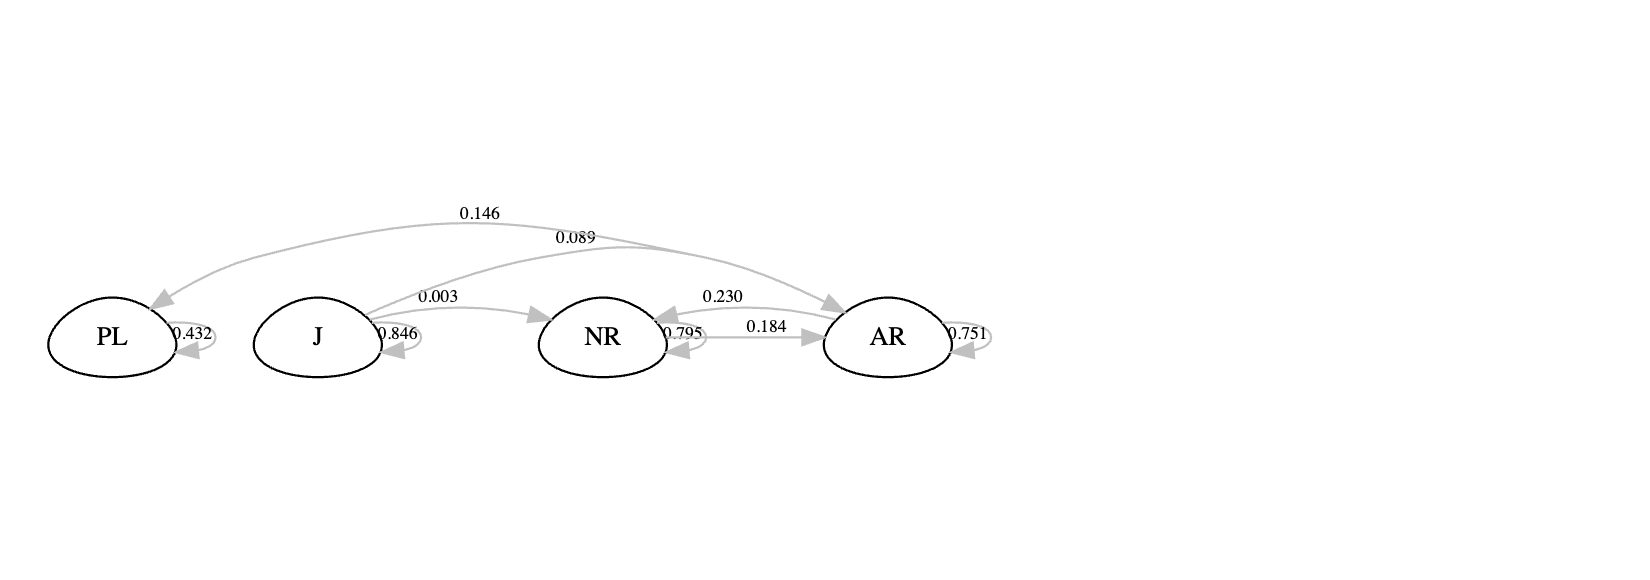
\includegraphics[keepaspectratio]{110-Propriedades_files/figure-pdf/Indice5-1.png}}

\begin{Shaded}
\begin{Highlighting}[]
\FunctionTok{isErgodic}\NormalTok{(Lr1\_No\_erg, }\AttributeTok{digits =} \DecValTok{4}\NormalTok{, }\AttributeTok{return.eigvec =} \ConstantTok{FALSE}\NormalTok{)}
\end{Highlighting}
\end{Shaded}

\begin{verbatim}
[1] FALSE
\end{verbatim}

\begin{center}\rule{0.5\linewidth}{0.5pt}\end{center}

\subsection{Elementos no negativos}\label{elementos-no-negativos}

Una matriz poblacional debe ser no negativa, lo que significa que todas
sus entradas son mayores o iguales a cero. ¿Por qué? Porque cada valor
representa el número o la proporción de individuos que pasan de una
etapa a otra. Tener valores negativos no tendría sentido biológico: no
puede haber ``menos'' individuos que los existentes.

Además, si la matriz tuviera elementos negativos:

\begin{itemize}
\tightlist
\item
  No podríamos comparar correctamente las categorías de edad o estado.
\item
  Sería imposible calcular la tasa de crecimiento poblacional.
\end{itemize}

En el caso de \emph{L. rubripetala}, la matriz cumple esta condición, ya
que todos sus valores son mayores o iguales a cero. En \textbf{R}, esto
se puede verificar con la función \texttt{IsPositive}, que devuelve:

\begin{itemize}
\tightlist
\item
  \texttt{TRUE} si la matriz es no negativa.
\item
  \texttt{FALSE} si contiene algún valor negativo.
\end{itemize}

\begin{Shaded}
\begin{Highlighting}[]
\CommentTok{\# No negativa }

\NormalTok{IsPositive }\OtherTok{\textless{}{-}} \ControlFlowTok{function}\NormalTok{(mat) \{}
  \ControlFlowTok{if}\NormalTok{ (}\FunctionTok{all}\NormalTok{(mat }\SpecialCharTok{\textgreater{}=} \DecValTok{0}\NormalTok{)) \{}
    \FunctionTok{return}\NormalTok{(}\ConstantTok{TRUE}\NormalTok{)}
\NormalTok{  \} }\ControlFlowTok{else}\NormalTok{ \{}
    \FunctionTok{return}\NormalTok{(}\ConstantTok{FALSE}\NormalTok{)}
\NormalTok{  \}}
\NormalTok{\}}

\FunctionTok{IsPositive}\NormalTok{(Lr1)}
\end{Highlighting}
\end{Shaded}

\begin{verbatim}
[1] TRUE
\end{verbatim}

A continuación se muestra un ejemplo de una matriz que no cumple la
propiedad de no negatividad. En este caso, el elemento ubicado en la
posición (4, 3) es negativo, lo que indica que la transición desde la
categoría adulto reproductivo hacia adulto no reproductivo tiene un
valor inválido.

Al evaluar esta matriz con la función \texttt{IsPositive} en \textbf{R},
el resultado es \texttt{FALSE}. Esto significa que:

\begin{itemize}
\tightlist
\item
  La matriz no es válida para el análisis de dinámica poblacional.
\item
  No se puede esperar que la población alcance una estructura estable ni
  una tasa de crecimiento constante a largo plazo.
\end{itemize}

\begin{Shaded}
\begin{Highlighting}[]
\CommentTok{\#Capturar los datos de la matriz para L. rubripetala (Tremblay et al. 2015)}
\NormalTok{Lr1\_No\_pos}\OtherTok{\textless{}{-}} \FunctionTok{matrix}\NormalTok{(}\FunctionTok{c}\NormalTok{(}\FloatTok{0.4324}\NormalTok{, }\DecValTok{0}\NormalTok{,      }\DecValTok{0}\NormalTok{,     }\FloatTok{0.146}\NormalTok{,}
               \FloatTok{0.3784}\NormalTok{, }\FloatTok{0.8459}\NormalTok{, }\DecValTok{0}\NormalTok{,     }\DecValTok{0}\NormalTok{,}
               \DecValTok{0}\NormalTok{,      }\FloatTok{0.0034}\NormalTok{, }\FloatTok{0.7954}\NormalTok{,}\SpecialCharTok{{-}}\FloatTok{0.2300}\NormalTok{,}
               \DecValTok{0}\NormalTok{,      }\FloatTok{0.0890}\NormalTok{, }\FloatTok{0.1841}\NormalTok{,}\FloatTok{0.7510}\NormalTok{), }\AttributeTok{byrow=}\ConstantTok{TRUE}\NormalTok{,}\AttributeTok{ncol=}\DecValTok{4}\NormalTok{)}

\FunctionTok{IsPositive}\NormalTok{(Lr1\_No\_pos)}
\end{Highlighting}
\end{Shaded}

\begin{verbatim}
[1] FALSE
\end{verbatim}

\begin{center}\rule{0.5\linewidth}{0.5pt}\end{center}

\subsection{Irreducibilidad}\label{irreducibilidad}

Una matriz de transición poblacional debe ser irreducible, lo que
significa que todas sus categorías están conectadas y existe al menos
una ruta que permite llegar desde cualquier estado a los demás. Esta
propiedad es esencial porque, si la matriz no es irreducible, la
población no podrá alcanzar una estructura estable ni una tasa de
crecimiento constante a largo plazo.

En el caso de \emph{L. rubripetala}, la matriz es irreducible: todas las
etapas del ciclo de vida están conectadas y existe una ruta entre ellas.
Para comprobar esta propiedad en \textbf{R}, se utiliza la función
\texttt{isIrreducible} del paquete \texttt{popdemo}, que devuelve:

\begin{itemize}
\tightlist
\item
  \texttt{TRUE} si la matriz es irreducible.
\item
  \texttt{FALSE} si no lo es.
\end{itemize}

Es importante destacar que no todas las matrices reducibles son
inválidas. En algunos casos, pueden aceptarse, por ejemplo, en especies
con etapas que no influyen en el crecimiento poblacional, como las fases
postreproductivas en mamíferos (humanos, ballenas, etc.).

En resumen, para \emph{L. rubripetala}, la función
\texttt{isIrreducible} devuelve \texttt{TRUE}, lo que confirma que todas
las categorías están conectadas y que la población puede alcanzar una
estructura estable y una tasa de crecimiento constante a largo plazo.

\begin{Shaded}
\begin{Highlighting}[]
\FunctionTok{isIrreducible}\NormalTok{(Lr1)}
\end{Highlighting}
\end{Shaded}

\begin{verbatim}
[1] TRUE
\end{verbatim}

A continuación se muestra un ejemplo de matriz en la que el cuarto
estadio no presenta valores de reproducción. Al evaluar esta matriz con
la función \texttt{isIrreducible} en \textbf{R}, el resultado es
\texttt{FALSE}.

¿Por qué ocurre esto? Porque no existe un vínculo entre la categoría
plántula y la categoría adulto reproductivo, lo que significa que la
presencia de plántulas en la población no contribuye a la reproducción.

Esta ausencia de conexión provoca dos problemas:

\begin{itemize}
\tightlist
\item
  Un ciclo de vida incompleto, como se observa en la imagen.
\item
  Una población que no podrá alcanzar una estructura estable ni una tasa
  de crecimiento constante a largo plazo.
\end{itemize}

\begin{Shaded}
\begin{Highlighting}[]
\NormalTok{Lr1\_Irr }\OtherTok{\textless{}{-}} \FunctionTok{matrix}\NormalTok{(}\FunctionTok{c}\NormalTok{(}\FloatTok{0.4324}\NormalTok{,  }\FloatTok{0.}\NormalTok{,       }\FloatTok{0.0}\NormalTok{,     }\DecValTok{0}\NormalTok{,}
                    \FloatTok{0.3784}\NormalTok{,  }\FloatTok{0.8459}\NormalTok{,   }\DecValTok{0}\NormalTok{,       }\DecValTok{0}\NormalTok{,}
                    \FloatTok{0.}\NormalTok{,      }\FloatTok{0.0034}\NormalTok{,   }\FloatTok{0.7954}\NormalTok{,  }\FloatTok{0.2300}\NormalTok{,}
                    \DecValTok{0}\NormalTok{,       }\FloatTok{0.0890}\NormalTok{,   }\FloatTok{0.1841}\NormalTok{,  }\FloatTok{0.7510}\NormalTok{), }\AttributeTok{byrow=}\ConstantTok{TRUE}\NormalTok{,}\AttributeTok{ncol=}\DecValTok{4}\NormalTok{)}

\FunctionTok{plot\_life\_cycle}\NormalTok{(Lr1\_Irr, }\AttributeTok{stages =}\NormalTok{ estadios, }\AttributeTok{fontsize =} \DecValTok{8}\NormalTok{)}
\end{Highlighting}
\end{Shaded}

\pandocbounded{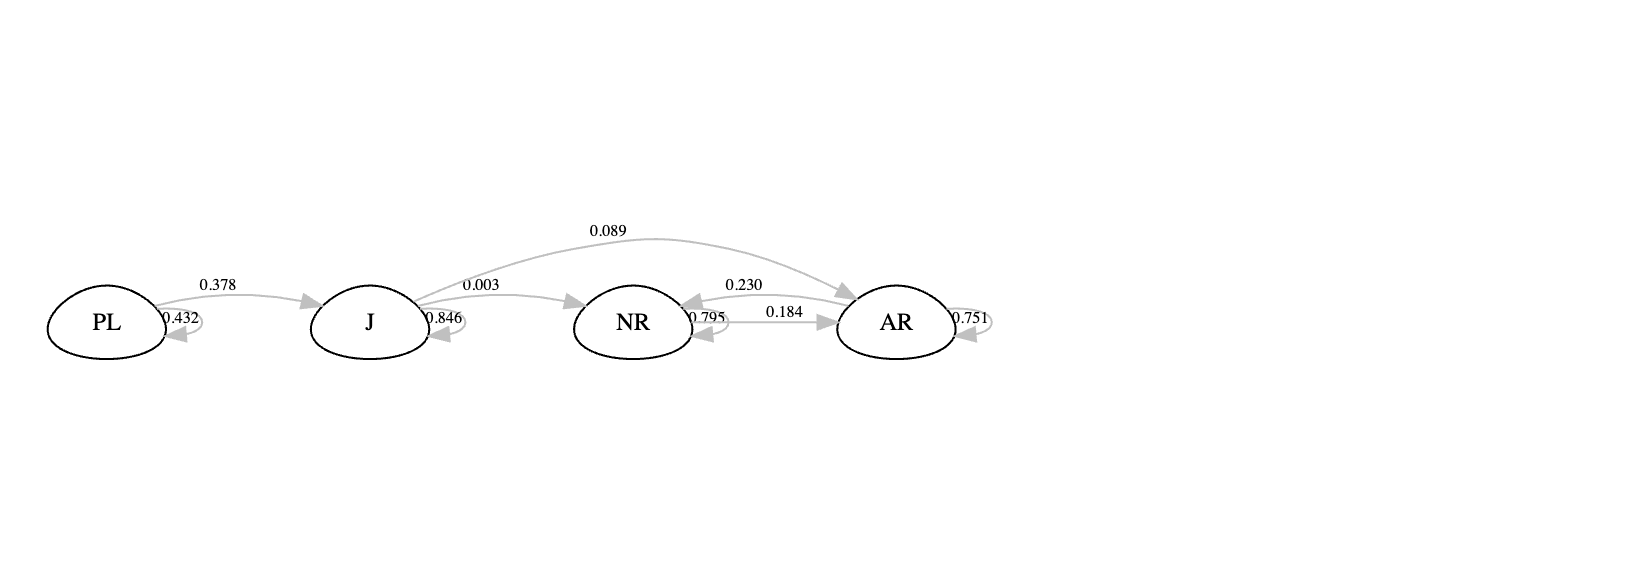
\includegraphics[keepaspectratio]{110-Propriedades_files/figure-pdf/unnamed-chunk-3-1.png}}

\begin{Shaded}
\begin{Highlighting}[]
\FunctionTok{isIrreducible}\NormalTok{(Lr1\_Irr)}
\end{Highlighting}
\end{Shaded}

\begin{verbatim}
[1] FALSE
\end{verbatim}

\begin{center}\rule{0.5\linewidth}{0.5pt}\end{center}

\subsection{Primitividad}\label{primitividad}

Una matriz de transición poblacional debe ser primitiva, lo que
significa que, al elevarla a potencias altas, se obtiene un único valor
positivo dominante (la tasa de crecimiento poblacional). Esta propiedad
es clave porque asegura que la población alcanzará una estructura
estable y una tasa de crecimiento constante a largo plazo.

En el caso de \emph{L. rubripetala}, la matriz es primitiva: al elevarla
a potencias altas, aparece un único valor positivo. En \textbf{R}, esto
se puede comprobar con la función \texttt{isPrimitive} del paquete
\texttt{popdemo}, que devuelve:

\begin{itemize}
\tightlist
\item
  \texttt{TRUE} si la matriz es primitiva.
\item
  \texttt{FALSE} si no lo es.
\end{itemize}

Una matriz no primitiva tendría una dinámica inestable a largo plazo,
como ocurre en poblaciones con comportamiento cíclico, donde las
proporciones entre categorías oscilan sin llegar a estabilizarse.

\begin{tcolorbox}[enhanced jigsaw, arc=.35mm, bottomrule=.15mm, bottomtitle=1mm, breakable, colback=white, colbacktitle=quarto-callout-note-color!10!white, colframe=quarto-callout-note-color-frame, coltitle=black, left=2mm, leftrule=.75mm, opacityback=0, opacitybacktitle=0.6, rightrule=.15mm, title=\textcolor{quarto-callout-note-color}{\faInfo}\hspace{0.5em}{Nota}, titlerule=0mm, toprule=.15mm, toptitle=1mm]

\textbf{Irreducible vs primitiva: la sutileza.}

\begin{itemize}
\tightlist
\item
  \textbf{Toda matriz primitiva es irreducible:} la primitividad
  requiere conectividad completa entre estadios \emph{más}
  aperiodicidad.
\item
  \textbf{No toda matriz irreducible es primitiva:} una matriz
  irreducible con estructura periódica (los individuos retornan al mismo
  estadio cada \(k\) pasos exactos) no converge a una estructura
  estable, sino que oscila. Su valor propio dominante no es único en
  módulo.
\end{itemize}

Por eso \texttt{popdemo} ofrece tanto \texttt{isIrreducible()} como
\texttt{isPrimitive()}: los modelos poblacionales bien comportados deben
pasar \textbf{ambos} chequeos.

\end{tcolorbox}

\begin{Shaded}
\begin{Highlighting}[]
\FunctionTok{isPrimitive}\NormalTok{(Lr1)}
\end{Highlighting}
\end{Shaded}

\begin{verbatim}
[1] TRUE
\end{verbatim}

\begin{tcolorbox}[enhanced jigsaw, arc=.35mm, bottomrule=.15mm, bottomtitle=1mm, breakable, colback=white, colbacktitle=quarto-callout-important-color!10!white, colframe=quarto-callout-important-color-frame, coltitle=black, left=2mm, leftrule=.75mm, opacityback=0, opacitybacktitle=0.6, rightrule=.15mm, title=\textcolor{quarto-callout-important-color}{\faExclamation}\hspace{0.5em}{Importante}, titlerule=0mm, toprule=.15mm, toptitle=1mm]

\textbf{Verifica estos cinco supuestos antes de calcular λ,
sensibilidades o elasticidades.} Si la matriz falla alguno, los análisis
posteriores pueden ser inválidos o difíciles de interpretar:

{\def\LTcaptype{none} % do not increment counter
\begin{longtable}[]{@{}
  >{\raggedright\arraybackslash}p{(\linewidth - 4\tabcolsep) * \real{0.3333}}
  >{\raggedright\arraybackslash}p{(\linewidth - 4\tabcolsep) * \real{0.3333}}
  >{\raggedright\arraybackslash}p{(\linewidth - 4\tabcolsep) * \real{0.3333}}@{}}
\toprule\noalign{}
\begin{minipage}[b]{\linewidth}\raggedright
Propiedad
\end{minipage} & \begin{minipage}[b]{\linewidth}\raggedright
Función en R
\end{minipage} & \begin{minipage}[b]{\linewidth}\raggedright
Por qué importa
\end{minipage} \\
\midrule\noalign{}
\endhead
\bottomrule\noalign{}
\endlastfoot
Cuadrada & \texttt{dim()} & Origen y destino deben ser comparables. \\
No negativa & \texttt{IsPositive()} & No tiene sentido biológico tener
entradas negativas. \\
Irreducible & \texttt{popdemo::isIrreducible()} & Asegura que todas las
etapas estén conectadas. \\
Primitiva & \texttt{popdemo::isPrimitive()} & Asegura una tasa de
crecimiento única (no oscilaciones). \\
Ergódica & \texttt{popbio::isErgodic()} & Asegura que la dinámica
asintótica no dependa del estado inicial. \\
\end{longtable}
}

Cuando alguna falla, conviene revisar el ciclo de vida y las matrices
originales (ver el capítulo de \hyperref[Ciclo_Vida]{Ciclos de Vida})
antes de pasar a análisis avanzados.

\end{tcolorbox}

\begin{center}\rule{0.5\linewidth}{0.5pt}\end{center}

\section{Índices de descripción de la matriz
poblacional}\label{uxedndices-de-descripciuxf3n-de-la-matriz-poblacional}

En esta sección se revisan los índices poblacionales obtenidos a partir
del análisis matricial, los cuales se estiman una vez que se ha
verificado que la matriz cumple con los supuestos. Estos índices
permiten comprender el comportamiento de la población a largo plazo y
anticipar cómo se espera que se comporte en el tiempo. Los índices que
se abordan a continuación son: \textbf{estructura estable},
\textbf{valor reproductivo}, \textbf{análisis de convergencia} y
\textbf{análisis de amortiguamiento}. Todos estos se calculan a partir
de la matriz de transición poblacional y del vector de la estructura
poblacional observada al inicio del estudio.

\begin{center}\rule{0.5\linewidth}{0.5pt}\end{center}

\subsection{Estructura estable}\label{estructura-estable}

La estructura poblacional estable (\(W\), también conocida como
eigenvector derecho) indica la proporción esperada de individuos en cada
categoría de edad o estado cuando la población ha alcanzado el
equilibrio a largo plazo. Por ejemplo, en \emph{L. rubripetala} se
espera que la estructura estable sea:

\begin{itemize}
\tightlist
\item
  Plántulas: 0.088
\item
  Juveniles: 0.206
\item
  Adultos no reproductivos: 0.369
\item
  Adultos reproductivos: 0.337
\end{itemize}

Este índice supone que la tasa de crecimiento poblacional (\(\lambda\))
se mantiene constante en el tiempo, lo cual solo ocurre bajo condiciones
ambientales estables. Sin embargo, en la naturaleza esto es poco común.
Además, la estructura estable asume que el periodo de muestreo y las
condiciones abióticas y bióticas son típicas y no cambian.

En la revisión de Williams y colaboradores (Williams et~al., 2011), se
reportó que más del 80\% de las poblaciones analizadas no cumplían con
la condición de estructura estable, especialmente en especies con
matrices grandes (n × n) y tiempos generacionales prolongados. De manera
similar, Tremblay (com. pers.) observó que la mayoría de las orquídeas
estudiadas no estaban en estructura estable al inicio del muestreo
poblacional.

\begin{tcolorbox}[enhanced jigsaw, arc=.35mm, bottomrule=.15mm, bottomtitle=1mm, breakable, colback=white, colbacktitle=quarto-callout-warning-color!10!white, colframe=quarto-callout-warning-color-frame, coltitle=black, left=2mm, leftrule=.75mm, opacityback=0, opacitybacktitle=0.6, rightrule=.15mm, title=\textcolor{quarto-callout-warning-color}{\faExclamationTriangle}\hspace{0.5em}{Advertencia}, titlerule=0mm, toprule=.15mm, toptitle=1mm]

\textbf{La estructura estable rara vez se observa en la naturaleza.}
Williams et al. (Williams et~al., 2011) reportan que más del 80\% de las
poblaciones analizadas no estaban en estructura estable, especialmente
en especies longevas con matrices grandes. Esto significa que las
proyecciones basadas en λ describen el comportamiento que
\textbf{tendría} la población si las condiciones se mantuvieran
constantes ---no necesariamente lo que observaremos en el corto plazo.
Para poblaciones lejos del equilibrio, conviene complementar λ con
análisis de dinámica transitoria (ver capítulo de
\href{112-Dinamica_de_Transiciones.qmd}{Dinámica de transiciones}).

\end{tcolorbox}

\begin{Shaded}
\begin{Highlighting}[]
\CommentTok{\#Estructura estable de estados}

\FunctionTok{stable.stage}\NormalTok{(Lr1)}
\end{Highlighting}
\end{Shaded}

\begin{verbatim}
        PL          J         NR         AR 
0.08614082 0.20286284 0.37222782 0.33876852 
\end{verbatim}

Uno puede visualizar la estructura poblacional usando el código
siguiente.

\begin{Shaded}
\begin{Highlighting}[]
\NormalTok{Wmax }\OtherTok{\textless{}{-}} \FunctionTok{stable.stage}\NormalTok{(Lr1)}
\NormalTok{Wdf }\OtherTok{=} \FunctionTok{data.frame}\NormalTok{(Wmax)}
\NormalTok{Wdf}\SpecialCharTok{$}\NormalTok{Categorias }\OtherTok{=} \FunctionTok{c}\NormalTok{(}
  \StringTok{"Plántulas"}\NormalTok{,}
  \StringTok{"Juveniles"}\NormalTok{,}
  \StringTok{"Adultos no reproductivos"}\NormalTok{,}
  \StringTok{"Adultos reproductivos"}
\NormalTok{)}
\NormalTok{Wdf}\SpecialCharTok{$}\NormalTok{Categorias }\OtherTok{=} \FunctionTok{factor}\NormalTok{(}
\NormalTok{  Wdf}\SpecialCharTok{$}\NormalTok{Categorias,}
  \AttributeTok{levels =} \FunctionTok{c}\NormalTok{(}
    \StringTok{"Plántulas"}\NormalTok{,}
    \StringTok{"Juveniles"}\NormalTok{,}
    \StringTok{"Adultos no reproductivos"}\NormalTok{,}
    \StringTok{"Adultos reproductivos"}
\NormalTok{  )}
\NormalTok{)}
\FunctionTok{library}\NormalTok{(ggplot2)}

\FunctionTok{ggplot}\NormalTok{(Wdf, }\FunctionTok{aes}\NormalTok{(}\AttributeTok{y =}\NormalTok{ Wmax, }\AttributeTok{x =}\NormalTok{ Categorias)) }\SpecialCharTok{+}
  \FunctionTok{geom\_bar}\NormalTok{(}\AttributeTok{stat =} \StringTok{"identity"}\NormalTok{, }\FunctionTok{aes}\NormalTok{(}\AttributeTok{fill =} \StringTok{"blue"}\NormalTok{)) }\SpecialCharTok{+}
  \FunctionTok{labs}\NormalTok{(}
    \AttributeTok{title =} \StringTok{"Estructura estable de estados esperada"}\NormalTok{,}
    \AttributeTok{x =} \StringTok{"Etapas"}\NormalTok{,}
    \AttributeTok{y =} \StringTok{"Proporción"}
\NormalTok{  ) }\SpecialCharTok{+}
  \FunctionTok{rlt\_style\_fill}\NormalTok{()}\SpecialCharTok{+}
  \FunctionTok{theme}\NormalTok{(}\AttributeTok{axis.text.x =} \FunctionTok{element\_text}\NormalTok{(}\AttributeTok{angle =} \DecValTok{45}\NormalTok{, }\AttributeTok{hjust =} \DecValTok{1}\NormalTok{))}\SpecialCharTok{+}
  \FunctionTok{theme}\NormalTok{(}\AttributeTok{legend.position=}\StringTok{"null"}\NormalTok{)}
\end{Highlighting}
\end{Shaded}

\pandocbounded{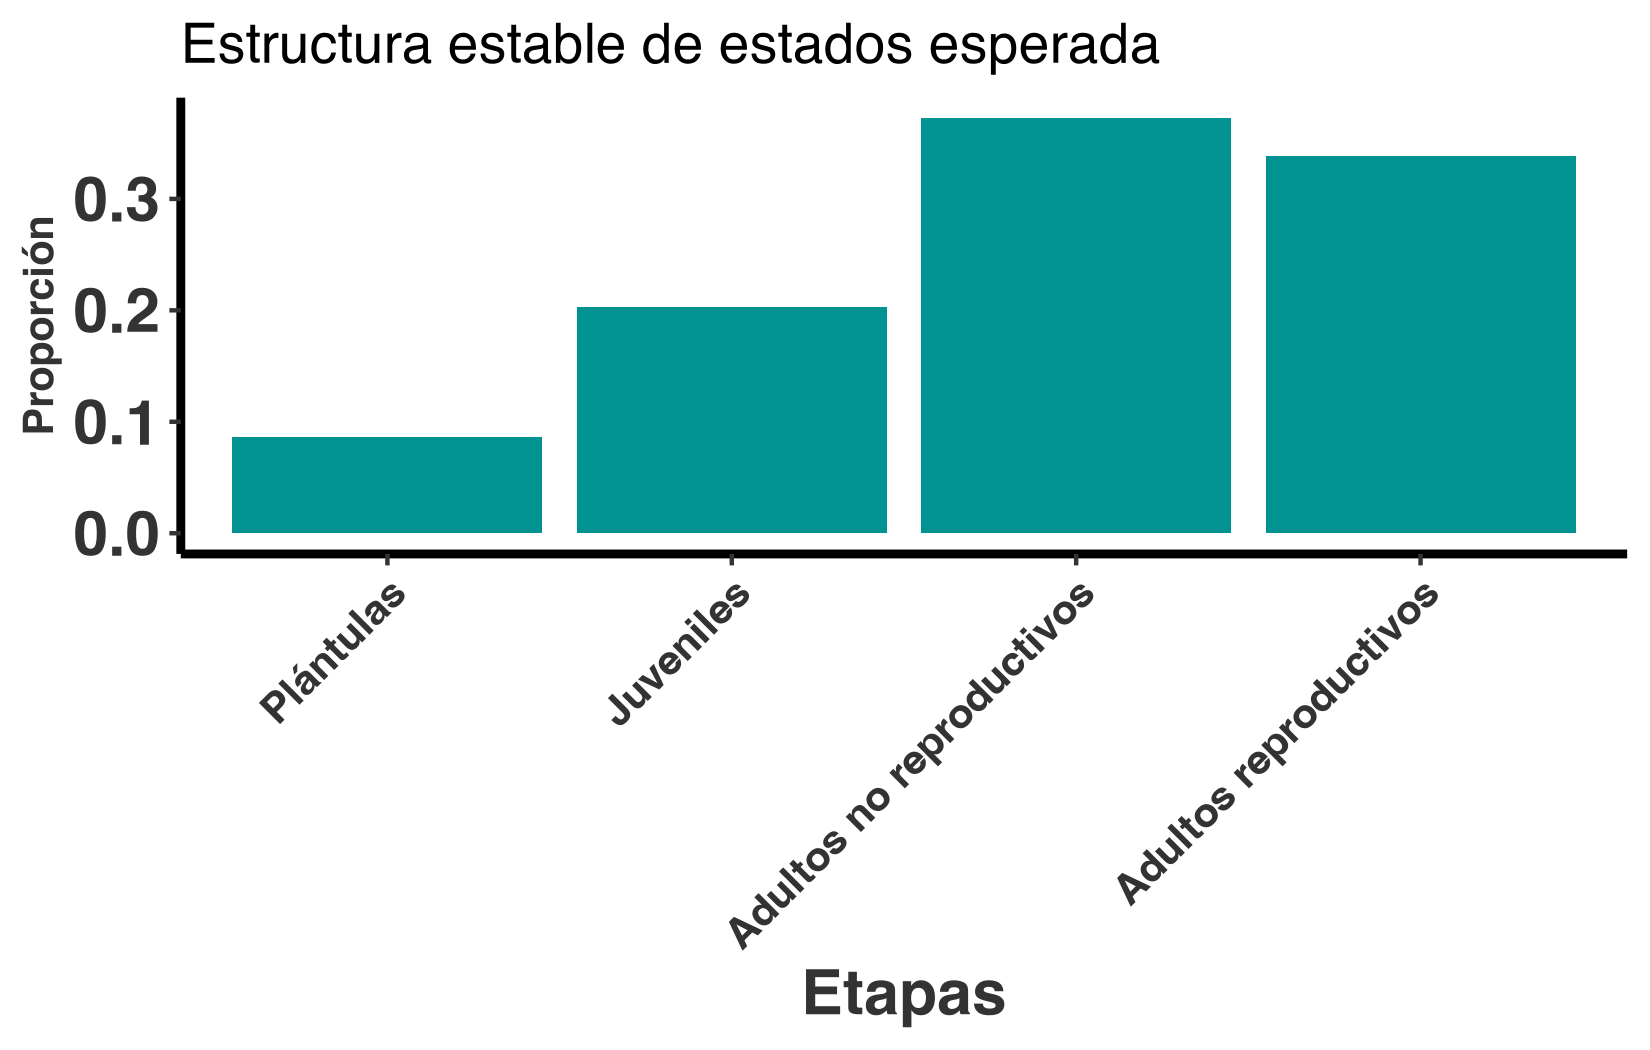
\includegraphics[keepaspectratio]{110-Propriedades_files/figure-pdf/Indice10-1.png}}

\begin{center}\rule{0.5\linewidth}{0.5pt}\end{center}

\subsection{Valor reproductivo}\label{valor-reproductivo}

\begin{figure}[H]

{\centering \pandocbounded{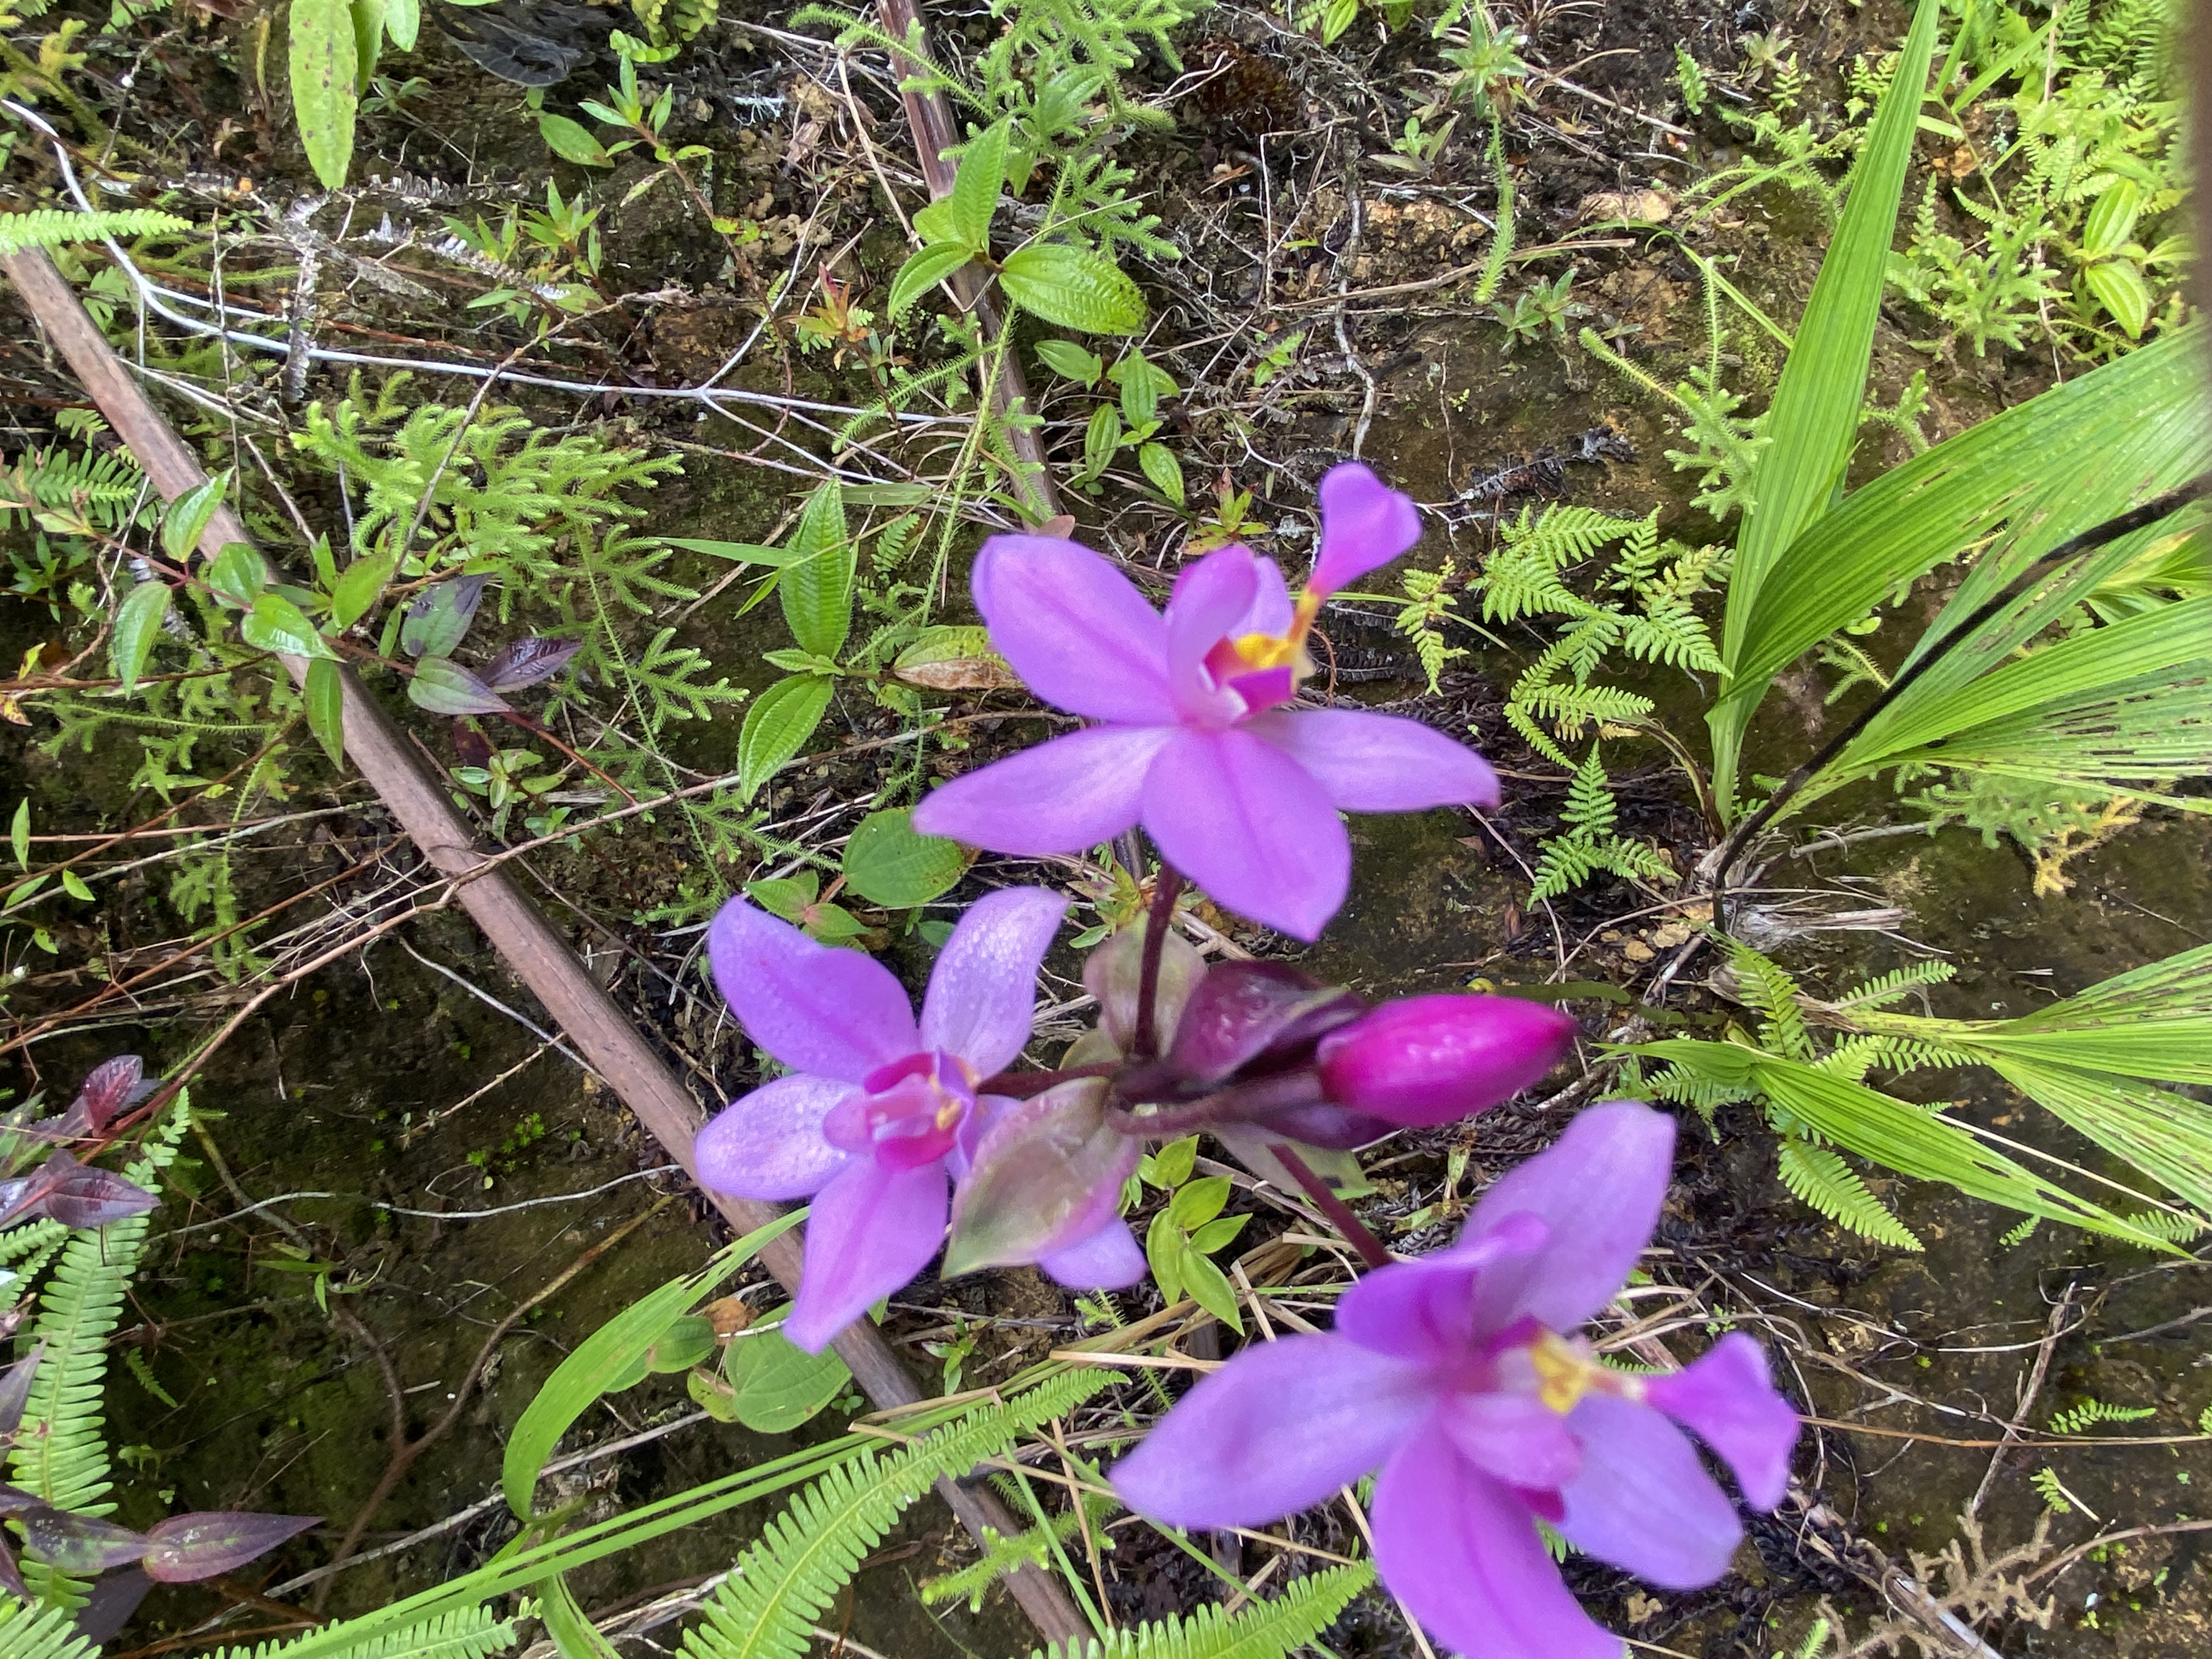
\includegraphics[keepaspectratio]{images/Spathoglottis_plicata_Tremblay.jpeg}}

}

\caption{\emph{Spathoglottis plicata}. Foto: Tremblay}

\end{figure}%

El valor reproductivo (\(v\), también llamado eigenvector izquierdo)
indica la contribución esperada de cada categoría de edad o estado a la
reproducción de la población.

En el caso de \emph{L. rubripetala}, los valores reproductivos esperados
son:

\begin{itemize}
\tightlist
\item
  Plántulas: 1.00
\item
  Juveniles: 1.52
\item
  Adultos no reproductivos: 2.32
\item
  Adultos reproductivos: 2.66
\end{itemize}

Este índice es muy útil porque muestra qué etapas son más importantes
para el crecimiento poblacional a largo plazo. La primera categoría
siempre tiene un valor de 1.00, ya que representa el inicio del ciclo de
vida y sirve como referencia para calcular los demás valores.

Además, el valor reproductivo ayuda a definir estrategias de manejo. Por
ejemplo:

\begin{itemize}
\item
  En \emph{Spathoglottis plicata}, una orquídea terrestre invasora, las
  acciones de control deberían enfocarse en las categorías con mayor
  valor reproductivo, porque son las que más contribuyen al crecimiento
  poblacional.
\item
  Por el contrario, si se busca remover individuos con el menor impacto
  posible, conviene actuar sobre las etapas con valores reproductivos
  bajos.
\end{itemize}

\begin{Shaded}
\begin{Highlighting}[]
\CommentTok{\# Valor reproductivo}

\FunctionTok{reproductive.value}\NormalTok{(Lr1)}
\end{Highlighting}
\end{Shaded}

\begin{verbatim}
      PL        J       NR       AR 
1.000000 1.517385 2.311211 2.651157 
\end{verbatim}

\begin{center}\rule{0.5\linewidth}{0.5pt}\end{center}

\subsection{\texorpdfstring{Análisis de convergencia y amortiguamiento
(\emph{damping
ratio})}{Análisis de convergencia y amortiguamiento (damping ratio)}}\label{anuxe1lisis-de-convergencia-y-amortiguamiento-damping-ratio}

El análisis de convergencia mide el tiempo esperado para que una
población alcance su estructura estable y un crecimiento asintótico
después de un disturbio. Es decir, indica qué tan rápido la población
regresa a su estructura estable tras una perturbación (Stott, Townley \&
Hodgson, 2011). Este comportamiento se cuantifica mediante el índice de
amortiguamiento (\emph{damping ratio}), que evalúa la influencia del
valor propio subdominante, \(\lambda_2\), durante el periodo de
convergencia.

El índice se expresa a través del cociente entre el valor propio
dominante, \(\lambda_1\), y el valor absoluto del subdominante:

\[\rho=\frac{\lambda_1}{\left|\lambda_2\right|}\]

donde \(\rho\) representa el índice de amortiguamiento, \(\lambda_1\)
corresponde al valor propio dominante de la matriz de transición
poblacional y \(\lambda_2\) al módulo del segundo valor propio más
grande. Este índice no tiene unidades y es independiente de la
estructura inicial de la población.

En el caso de \emph{L. rubripetala}, al calcular los valores propios de
la matriz con la función \texttt{eigen}, se obtiene un valor dominante
de \(\lambda_1 = 1.00658\) y un valor subdominante de
\(\lambda_2 = 0.8322\). De esta manera, el índice de amortiguamiento es:

\[
\rho = \frac{\lambda_1}{|\lambda_2|} = \frac{1.00658}{|0.83220|} \approx 1.21
\]

El valor obtenido indica que la población converge hacia su estructura
estable tras un disturbio; aunque, lentamente.

Es importante señalar que la interpretación de este índice depende de la
escala temporal con que se construyó la matriz. Si bien la mayoría de
los estudios poblacionales utilizan datos anuales ({Crone et~al.},
2011), también existen estudios con periodos de muestreo mensuales,
bimensuales, estacionales o bianuales, los cuales se establecen de
acuerdo con el ciclo de vida de la especie estudiada.

\begin{Shaded}
\begin{Highlighting}[]
\FunctionTok{eigen}\NormalTok{(Lr1)}\SpecialCharTok{$}\NormalTok{values }\CommentTok{\# la lista de valores propios de la matriz Lr1}
\end{Highlighting}
\end{Shaded}

\begin{verbatim}
[1] 1.0065785+0.00000000i 0.8322016+0.00000000i 0.4929600+0.06290472i
[4] 0.4929600-0.06290472i
\end{verbatim}

\begin{Shaded}
\begin{Highlighting}[]
\NormalTok{DR }\OtherTok{=} \FunctionTok{eigen}\NormalTok{(Lr1)}\SpecialCharTok{$}\NormalTok{values[}\DecValTok{1}\NormalTok{] }\SpecialCharTok{/} \FunctionTok{abs}\NormalTok{(}\FunctionTok{eigen}\NormalTok{(Lr1)}\SpecialCharTok{$}\NormalTok{values[}\DecValTok{2}\NormalTok{])}

\NormalTok{DR}
\end{Highlighting}
\end{Shaded}

\begin{verbatim}
[1] 1.209537+0i
\end{verbatim}

\begin{Shaded}
\begin{Highlighting}[]
\FunctionTok{dr}\NormalTok{(Lr1) }\CommentTok{\# usando la función "dr" para "damping ratio" en el paquete "popdemo"}
\end{Highlighting}
\end{Shaded}

\begin{verbatim}
[1] 1.209537
\end{verbatim}

\subsection{Graficación del índice de
amortiguamiento}\label{graficaciuxf3n-del-uxedndice-de-amortiguamiento}

El comportamiento del índice de amortiguamiento se puede visualizar
mediante una gráfica de líneas, que muestra cómo responde un sistema
ante un cambio súbito (un ``paso de entrada'') y cómo varía esa
respuesta en el tiempo según diferentes niveles de amortiguamiento.

Para facilitar la comprensión, en el siguiente bloque se incluye el
código que genera una gráfica ilustrando el comportamiento de una
población perturbada:

\begin{Shaded}
\begin{Highlighting}[]
\FunctionTok{library}\NormalTok{(ggplot2)}

\CommentTok{\# {-}{-}{-} Definir los parametros {-}{-}{-}}
\CommentTok{\# Población inicial en el tiempo t=0. Ese el punto de equilibrio inicial.}
\NormalTok{poblacion\_inicial }\OtherTok{\textless{}{-}} \DecValTok{1000}

\CommentTok{\# Factores de amortiguamiento para graficar.}
\CommentTok{\# 0,3 = Subamortiguado (oscila)}
\CommentTok{\# 1,0 = Críticamente amortiguado (retorno más rápido sin oscilación)}
\CommentTok{\# 2,0 = Sobreamortiguado (retorno lento sin oscilación)}
\NormalTok{amortiguamiento }\OtherTok{\textless{}{-}} \FunctionTok{c}\NormalTok{(}\FloatTok{0.3}\NormalTok{, }\FloatTok{1.0}\NormalTok{, }\FloatTok{2.0}\NormalTok{, }\FloatTok{3.0}\NormalTok{)}

\CommentTok{\# Frecuencia de la oscilación (omega\_n).}
\NormalTok{frecuencia }\OtherTok{\textless{}{-}} \FloatTok{0.5}

\CommentTok{\# Tiempo total para la simulación}
\NormalTok{tiempo\_total }\OtherTok{\textless{}{-}} \DecValTok{50}

\CommentTok{\# Paso de tiempo para la simulación (más pequeño para una curva más suave)}
\NormalTok{etapa\_tiempo }\OtherTok{\textless{}{-}} \FloatTok{0.1}

\CommentTok{\# {-}{-}{-} Generar los datos de oscilación amortiguada para múltiples coeficientes {-}{-}{-}}
\CommentTok{\# Crear un data frame vacío para almacenar todos los datos}
\NormalTok{todo\_data\_df }\OtherTok{\textless{}{-}} \FunctionTok{data.frame}\NormalTok{()}

\CommentTok{\# Recorra cada relación de amortiguamiento para generar los datos}
\ControlFlowTok{for}\NormalTok{ (zeta }\ControlFlowTok{in}\NormalTok{ amortiguamiento) \{}
 \CommentTok{\# Crear una secuencia de puntos de tiempo}
\NormalTok{  time\_points }\OtherTok{\textless{}{-}} \FunctionTok{seq}\NormalTok{(}\DecValTok{0}\NormalTok{, tiempo\_total, }\AttributeTok{by =}\NormalTok{ etapa\_tiempo)}

  \CommentTok{\# Calcular la población en cada punto de tiempo según el coeficiente de amortiguamiento.}
  \CommentTok{\# La forma matemática de la respuesta al escalón cambia según el coeficiente de amortiguamiento.}

  \ControlFlowTok{if}\NormalTok{ (zeta }\SpecialCharTok{\textless{}} \DecValTok{1}\NormalTok{) \{}
    \CommentTok{\# Underdamped case: damped sine wave}
\NormalTok{    omega\_d }\OtherTok{\textless{}{-}}\NormalTok{ frecuencia }\SpecialCharTok{*} \FunctionTok{sqrt}\NormalTok{(}\DecValTok{1} \SpecialCharTok{{-}}\NormalTok{ zeta}\SpecialCharTok{\^{}}\DecValTok{2}\NormalTok{)}
\NormalTok{    population\_data }\OtherTok{\textless{}{-}}\NormalTok{ poblacion\_inicial }\SpecialCharTok{*}
\NormalTok{      (}\DecValTok{1} \SpecialCharTok{{-}}
        \FunctionTok{exp}\NormalTok{(}\SpecialCharTok{{-}}\NormalTok{zeta }\SpecialCharTok{*}\NormalTok{ frecuencia }\SpecialCharTok{*}\NormalTok{ time\_points) }\SpecialCharTok{*}
\NormalTok{          (}\FunctionTok{cos}\NormalTok{(omega\_d }\SpecialCharTok{*}\NormalTok{ time\_points) }\SpecialCharTok{+}
\NormalTok{            (zeta }\SpecialCharTok{/} \FunctionTok{sqrt}\NormalTok{(}\DecValTok{1} \SpecialCharTok{{-}}\NormalTok{ zeta}\SpecialCharTok{\^{}}\DecValTok{2}\NormalTok{)) }\SpecialCharTok{*} \FunctionTok{sin}\NormalTok{(omega\_d }\SpecialCharTok{*}\NormalTok{ time\_points)))}
\NormalTok{  \} }\ControlFlowTok{else} \ControlFlowTok{if}\NormalTok{ (zeta }\SpecialCharTok{==} \DecValTok{1}\NormalTok{) \{}
    \CommentTok{\# Critically Damped case}
\NormalTok{    population\_data }\OtherTok{\textless{}{-}}\NormalTok{ poblacion\_inicial }\SpecialCharTok{*}
\NormalTok{      (}\DecValTok{1} \SpecialCharTok{{-}} \FunctionTok{exp}\NormalTok{(}\SpecialCharTok{{-}}\NormalTok{frecuencia }\SpecialCharTok{*}\NormalTok{ time\_points) }\SpecialCharTok{*}\NormalTok{ (}\DecValTok{1} \SpecialCharTok{+}\NormalTok{ frecuencia }\SpecialCharTok{*}\NormalTok{ time\_points))}
\NormalTok{  \} }\ControlFlowTok{else}\NormalTok{ \{}
    \CommentTok{\# Overdamped case}
\NormalTok{    s1 }\OtherTok{\textless{}{-}} \SpecialCharTok{{-}}\NormalTok{zeta }\SpecialCharTok{*}\NormalTok{ frecuencia }\SpecialCharTok{+}\NormalTok{ frecuencia }\SpecialCharTok{*} \FunctionTok{sqrt}\NormalTok{(zeta}\SpecialCharTok{\^{}}\DecValTok{2} \SpecialCharTok{{-}} \DecValTok{1}\NormalTok{)}
\NormalTok{    s2 }\OtherTok{\textless{}{-}} \SpecialCharTok{{-}}\NormalTok{zeta }\SpecialCharTok{*}\NormalTok{ frecuencia }\SpecialCharTok{{-}}\NormalTok{ frecuencia }\SpecialCharTok{*} \FunctionTok{sqrt}\NormalTok{(zeta}\SpecialCharTok{\^{}}\DecValTok{2} \SpecialCharTok{{-}} \DecValTok{1}\NormalTok{)}
\NormalTok{    population\_data }\OtherTok{\textless{}{-}}\NormalTok{ poblacion\_inicial }\SpecialCharTok{*}
\NormalTok{      (}\DecValTok{1} \SpecialCharTok{{-}}
\NormalTok{        (s2 }\SpecialCharTok{*} \FunctionTok{exp}\NormalTok{(s1 }\SpecialCharTok{*}\NormalTok{ time\_points) }\SpecialCharTok{{-}}\NormalTok{ s1 }\SpecialCharTok{*} \FunctionTok{exp}\NormalTok{(s2 }\SpecialCharTok{*}\NormalTok{ time\_points)) }\SpecialCharTok{/}\NormalTok{ (s2 }\SpecialCharTok{{-}}\NormalTok{ s1))}
\NormalTok{  \}}

  \CommentTok{\# Añadir los datos del coeficiente actual a un data frame temporal}
\NormalTok{  temp\_df }\OtherTok{\textless{}{-}} \FunctionTok{data.frame}\NormalTok{(}
    \AttributeTok{Time =}\NormalTok{ time\_points,}
    \AttributeTok{Population =}\NormalTok{ population\_data,}
    \AttributeTok{DampingRatio =} \FunctionTok{factor}\NormalTok{(zeta) }\CommentTok{\# Store damping ratio as a factor for coloring}
\NormalTok{  )}

  \CommentTok{\# Unir el data frame temporal al data frame principal}
\NormalTok{  todo\_data\_df }\OtherTok{\textless{}{-}} \FunctionTok{rbind}\NormalTok{(todo\_data\_df, temp\_df)}
\NormalTok{\}}

\CommentTok{\# {-}{-}{-} Crear el gráfico usando ggplot2 {-}{-}{-}}
\FunctionTok{ggplot}\NormalTok{(todo\_data\_df, }\FunctionTok{aes}\NormalTok{(}\AttributeTok{x =}\NormalTok{ Time, }\AttributeTok{y =}\NormalTok{ Population, }\AttributeTok{color =}\NormalTok{ DampingRatio)) }\SpecialCharTok{+}
  \CommentTok{\# Añadir las líneas para cada coeficiente de amortiguamiento}
  \FunctionTok{geom\_line}\NormalTok{(}\AttributeTok{linewidth =} \FloatTok{1.2}\NormalTok{) }\SpecialCharTok{+}
  \CommentTok{\# Establecer el título y las etiquetas}
\FunctionTok{labs}\NormalTok{(}
  \AttributeTok{title =} \StringTok{"El efecto de amortiguamiento }\SpecialCharTok{\textbackslash{}n}\StringTok{ sobre el tamaño de población"}\NormalTok{,}
  \AttributeTok{subtitle =} \StringTok{"La población se estabiliza a un equilibrio de 1000"}\NormalTok{,}
  \AttributeTok{x =} \StringTok{"Tiempo"}\NormalTok{,}
  \AttributeTok{y =} \StringTok{"Tamaño poblacional"}\NormalTok{,}
  \AttributeTok{color =} \FunctionTok{expression}\NormalTok{(}\StringTok{"Amortiguamiento ("} \SpecialCharTok{*}\NormalTok{ zeta }\SpecialCharTok{*} \StringTok{")"}\NormalTok{)}
\NormalTok{) }\SpecialCharTok{+}
  \CommentTok{\# Personalizar el tema del gráfico para mejor estética}
  \FunctionTok{rlt\_style\_colour}\NormalTok{() }\SpecialCharTok{+}
  \FunctionTok{theme\_minimal}\NormalTok{(}\AttributeTok{base\_size =} \DecValTok{14}\NormalTok{) }\SpecialCharTok{+}
  \FunctionTok{theme}\NormalTok{(}
    \AttributeTok{plot.title =} \FunctionTok{element\_text}\NormalTok{(}\AttributeTok{hjust =} \FloatTok{0.5}\NormalTok{, }\AttributeTok{face =} \StringTok{"bold"}\NormalTok{),}
    \AttributeTok{plot.subtitle =} \FunctionTok{element\_text}\NormalTok{(}\AttributeTok{hjust =} \FloatTok{0.5}\NormalTok{),}
    \AttributeTok{axis.title =} \FunctionTok{element\_text}\NormalTok{(}\AttributeTok{face =} \StringTok{"bold"}\NormalTok{)}
\NormalTok{  )}
\end{Highlighting}
\end{Shaded}

\pandocbounded{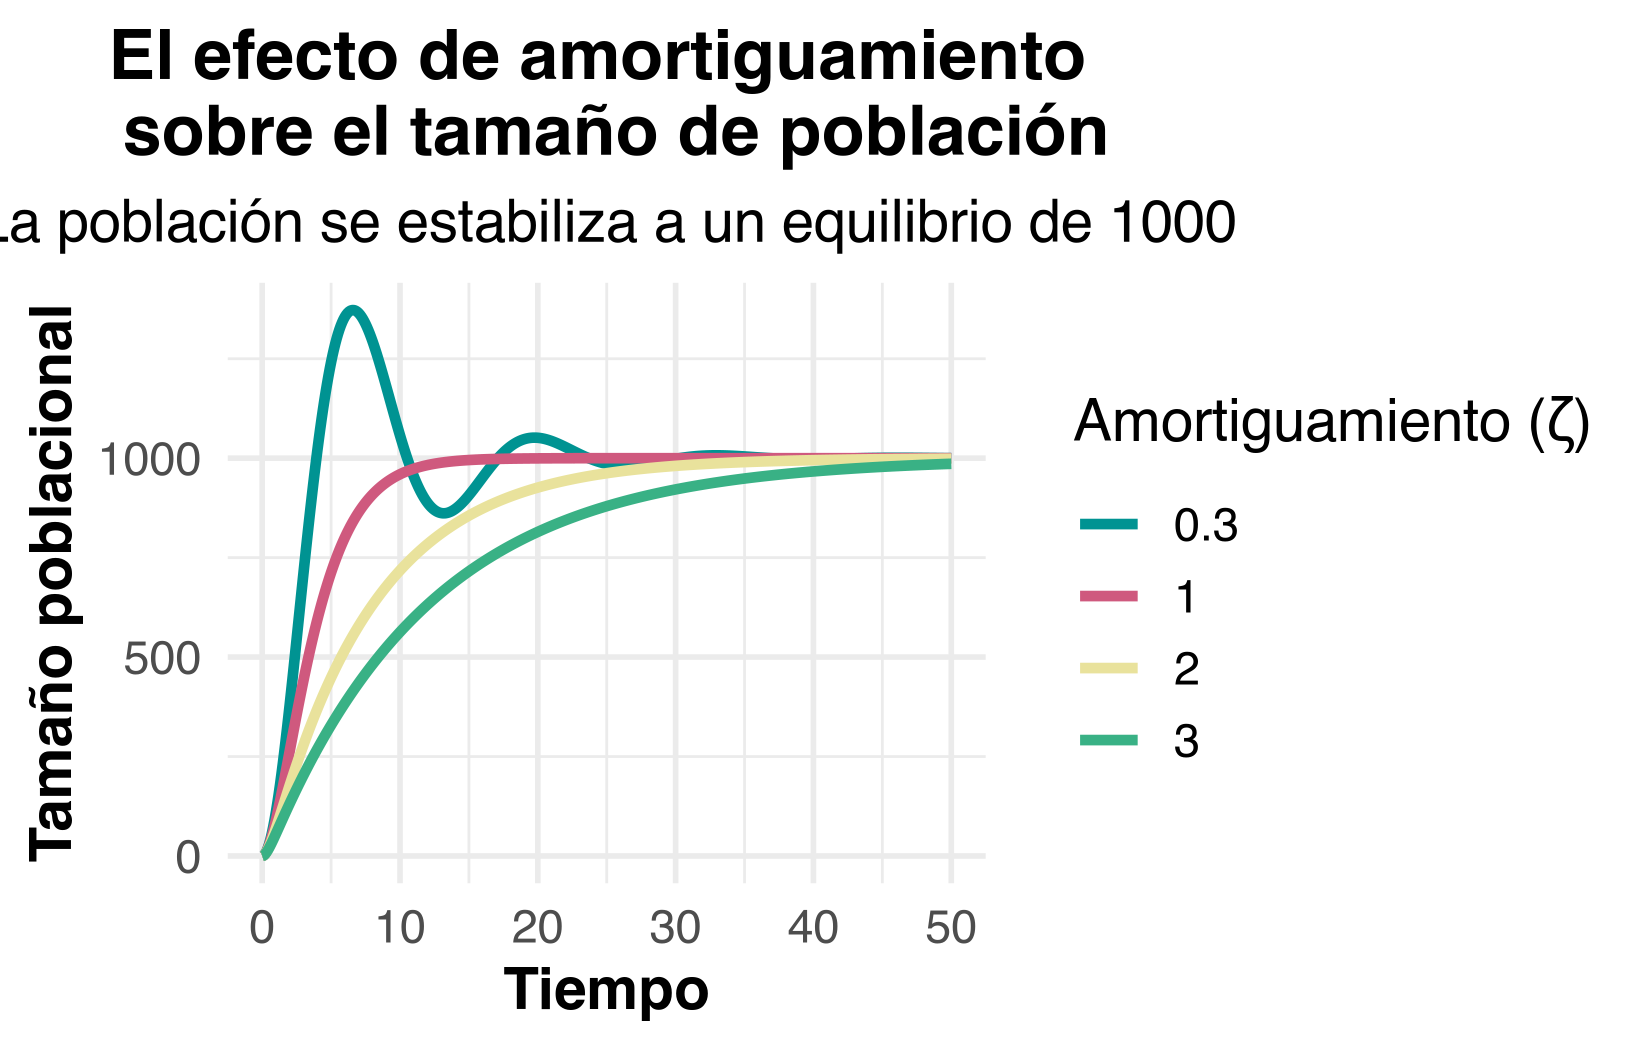
\includegraphics[keepaspectratio]{110-Propriedades_files/figure-pdf/Indice13-1.png}}

\subsection{Interpretación del gráfico de
amortiguamiento}\label{interpretaciuxf3n-del-gruxe1fico-de-amortiguamiento}

La figura resultante ilustra el efecto de diferentes coeficientes de
amortiguamiento en la respuesta de una población a un cambio súbito. El
gráfico muestra cuatro comportamientos distintos para la población
perturbada y su retorno a un estado de equilibrio, correspondiente a un
tamaño poblacional de 1000 individuos.

La respuesta de la población ante cuatro índices de amortiguamiento es
la siguiente:

\begin{itemize}
\tightlist
\item
  \textbf{Subamortiguado} (\(\zeta = 0.3\)): Esta es la respuesta
  oscilante. El sistema sobrepasa el punto de equilibrio y luego oscila;
  con el tiempo la amplitud de las oscilaciones disminuye gradualmente
  hasta estabilizarse en el equilibrio.
\item
  \textbf{Amortiguado críticamente} (\(\zeta = 1.0\)): Esta es la
  respuesta más rápida, la cual alcanza el equilibrio sin oscilaciones
  ni sobreamortiguaciones. Se considera la respuesta ideal para sistemas
  que requieren un retorno rápido y estable al valor objetivo.
\item
  \textbf{Sobreamortiguado} (\(\zeta = 2.0\)): Esta respuesta es lenta y
  se aproxima al punto de equilibrio sin oscilaciones. En comparación
  con el caso críticamente amortiguado, tarda mucho más en
  estabilizarse, ya que la fuerza de amortiguamiento es muy grande.
\item
  \textbf{Sobreamortiguado} (\(\zeta = 3.0\)): Similar al caso anterior,
  pero con un amortiguamiento aún mayor. La respuesta es muy lenta y se
  acerca al equilibrio de manera gradual sin oscilaciones.
\end{itemize}

\begin{tcolorbox}[enhanced jigsaw, arc=.35mm, bottomrule=.15mm, bottomtitle=1mm, breakable, colback=white, colbacktitle=quarto-callout-note-color!10!white, colframe=quarto-callout-note-color-frame, coltitle=black, left=2mm, leftrule=.75mm, opacityback=0, opacitybacktitle=0.6, rightrule=.15mm, title=\textcolor{quarto-callout-note-color}{\faInfo}\hspace{0.5em}{Nota}, titlerule=0mm, toprule=.15mm, toptitle=1mm]

\textbf{Cuatro regímenes de amortiguamiento.}

{\def\LTcaptype{none} % do not increment counter
\begin{longtable}[]{@{}
  >{\raggedright\arraybackslash}p{(\linewidth - 4\tabcolsep) * \real{0.3333}}
  >{\raggedright\arraybackslash}p{(\linewidth - 4\tabcolsep) * \real{0.3333}}
  >{\raggedright\arraybackslash}p{(\linewidth - 4\tabcolsep) * \real{0.3333}}@{}}
\toprule\noalign{}
\begin{minipage}[b]{\linewidth}\raggedright
ζ
\end{minipage} & \begin{minipage}[b]{\linewidth}\raggedright
Régimen
\end{minipage} & \begin{minipage}[b]{\linewidth}\raggedright
Comportamiento
\end{minipage} \\
\midrule\noalign{}
\endhead
\bottomrule\noalign{}
\endlastfoot
\textless{} 1 & \textbf{Subamortiguado} & Sobrepasa el equilibrio y
oscila; la amplitud decrece con el tiempo. \\
= 1 & \textbf{Críticamente amortiguado} & Retorno más rápido posible sin
oscilaciones. \\
\textgreater{} 1 (moderado) & \textbf{Sobreamortiguado} & Retorno lento
sin oscilaciones; la fuerza de amortiguamiento es alta. \\
≫ 1 & \textbf{Muy sobreamortiguado} & Retorno extremadamente lento; el
sistema apenas reacciona. \\
\end{longtable}
}

En poblaciones reales, la mayoría de las matrices de proyección se
encuentran en el régimen sobreamortiguado: regresan al equilibrio sin
oscilar, pero pueden tardar muchas generaciones.

\end{tcolorbox}

\subsection{Tiempo de convergencia}\label{tiempo-de-convergencia}

El tiempo de convergencia es el periodo estimado que tarda la población
en alcanzar su estructura estable. Este índice es relevante porque
facilita entender el comportamiento poblacional a largo plazo. En
\textbf{R} este cálculo puede realizarse con dos funciones del paquete
\texttt{popdemo}: \texttt{dr} y \texttt{convt}. La función \texttt{dr}
calcula el amortiguamiento, y a partir de éste puede estimarse el tiempo
de convergencia de la siguiente manera:

\[
t = \frac{\log(x)}{\log(\rho)}
\]

donde

\begin{itemize}
\tightlist
\item
  \(\rho\) es el índice de amortiguamiento (\emph{damping ratio},
  \(\rho = \lambda_1 / |\lambda_2|\))
\item
  \(x\) es el factor por el cual la influencia del valor propio
  dominante debe superar a la del subdominante (por ejemplo, \(x = 10\)
  significa ``tiempo hasta que el dominante pese 10 veces más que el
  subdominante'')
\item
  \(t\) representa el tiempo en la misma unidad en que se construyó la
  matriz (días, meses, años, etc.).
\end{itemize}

Mientras mayor sea \(\rho\), más rápida será la convergencia: una matriz
con \(\rho = 2\) converge mucho más rápido que una con \(\rho = 1.05\).
El análisis de amortiguamiento estima la rapidez con la que una
población converge a su estructura estable después de un disturbio
(Jiang et~al., 2020). Cabe señalar que se ha demostrado que existe una
relación entre el índice de amortiguamiento y el tiempo generacional de
una especie (Jiang et~al., 2020).

\begin{Shaded}
\begin{Highlighting}[]
\FunctionTok{dr}\NormalTok{(Lr1, }\AttributeTok{return.time =} \ConstantTok{TRUE}\NormalTok{, }\AttributeTok{x =} \DecValTok{10}\NormalTok{) }\CommentTok{\# cuanto tiempo toma aumentar la población de veces }
\end{Highlighting}
\end{Shaded}

\begin{verbatim}
$dr
[1] 1.209537

$t
[1] 12.10374
\end{verbatim}

A partir de la función \texttt{convt} del paquete \texttt{popdemo} se
puede estimar el tiempo esperado en que una población alcanza su
estructura estable, considerando la estructura poblacional observada al
inicio del estudio. Esta función simula el modelo y determina
manualmente cuándo la población converge, dado un nivel de exactitud
específico (\emph{accuracy}). Entre más estricta sea la exactitud, mayor
será el tiempo de convergencia. Para utilizar esta función es necesario
indicar la estructura inicial, es decir, el número de individuos en cada
estadio. En el caso de \emph{L. rubripetala} se espera que el tiempo de
convergencia sea de 18 ciclos (meses) para alcanzar su estructura
estable.

Por ejemplo, si se comienza con una población inicial de 8, 20, 27 y 34
individuos en las categorías de plántulas, juveniles, adultos no
reproductivos y adultos reproductivos, respectivamente, la población
alcanzaría en 6 meses, aproximadamente, la estructura estable. En
contraste, si la población inicial estuviera sesgada (compuesta
únicamente por plántulas, por ejemplo), el tiempo de convergencia sería
mucho mayor. Este enfoque resulta muy útil al definir estrategias de
conservación; por ejemplo, al establecer una nueva población con una
distribución inicial determinada.

\begin{tcolorbox}[enhanced jigsaw, arc=.35mm, bottomrule=.15mm, bottomtitle=1mm, breakable, colback=white, colbacktitle=quarto-callout-tip-color!10!white, colframe=quarto-callout-tip-color-frame, coltitle=black, left=2mm, leftrule=.75mm, opacityback=0, opacitybacktitle=0.6, rightrule=.15mm, title=\textcolor{quarto-callout-tip-color}{\faLightbulb}\hspace{0.5em}{Recomendación}, titlerule=0mm, toprule=.15mm, toptitle=1mm]

\textbf{La estructura inicial determina cuánto tarda la convergencia.}
Para la misma matriz de \emph{L. rubripetala}:

\begin{itemize}
\tightlist
\item
  Estructura inicial cercana a la estable (ej. 8, 20, 27, 34):
  convergencia en \textasciitilde6 meses.
\item
  Estructura inicial moderadamente sesgada: \textasciitilde18 meses.
\item
  Estructura completamente sesgada (sólo plántulas): \textasciitilde25
  meses.
\end{itemize}

Esto tiene implicaciones prácticas en conservación: si introduces una
nueva población o una población en restauración, la composición inicial
determina cuándo el modelo asintótico empieza a aplicar. Para acelerar
la convergencia, conviene introducir individuos en proporciones cercanas
a la estructura estable cuando sea factible.

\end{tcolorbox}

\begin{Shaded}
\begin{Highlighting}[]
\NormalTok{n0 }\OtherTok{\textless{}{-}} \FunctionTok{c}\NormalTok{(}\DecValTok{8}\NormalTok{, }\DecValTok{20}\NormalTok{, }\DecValTok{27}\NormalTok{, }\DecValTok{34}\NormalTok{) }\CommentTok{\# la estructura de la población inicial}

\FunctionTok{convt}\NormalTok{(Lr1, }\AttributeTok{accuracy =} \FloatTok{1e{-}4}\NormalTok{, }\AttributeTok{vector =}\NormalTok{ n0, }\AttributeTok{iterations =} \DecValTok{10000}\NormalTok{) }\CommentTok{\# la estructura poblacional inicial}
\end{Highlighting}
\end{Shaded}

\begin{verbatim}
[1] 19
\end{verbatim}

Dado que el tiempo de convergencia es un índice que representa el
periodo esperado para que una población alcance su estructura estable,
se puede calcular variando la cantidad de individuos en las diferentes
edades o estados al llevar a cabo una simulación.

Por ejemplo, se estima que \emph{L. rubripetala} alcanzaría la
estructura estable en 25 meses, si la población inicia con una población
sesgada a plántulas (n = 1000) y, por lo tanto, sin la presencia de
individuos de los estados posteriores.

\subsection{Graficación del tiempo de convergencia al estado estable de
cada etapa de
vida}\label{graficaciuxf3n-del-tiempo-de-convergencia-al-estado-estable-de-cada-etapa-de-vida}

La población comienza en cada etapa con 100 individuos y se simula
durante 22 pasos de tiempo. El gráfico resultante muestra cómo la
población converge a su estructura estable a lo largo del tiempo, con
cada etapa representada por una línea de color diferente. La línea
horizontal indica el valor de la proporción de la etapa estable y la
línea vertical representa el tiempo en que se espera que la etapa llegue
a su nivel de estructura estable.

Nota que si las condiciones se mantienen iguales en el tiempo, se espera
que la población converja a una estructura estable, es decir, que la
proporción de individuos en cada etapa se mantenga constante a lo largo
del tiempo. En este caso, la proporción de individuos en cada etapa
converge a 0.088, 0.206, 0.369 y 0.337 para las categorías de plántulas,
juveniles, adultos no reproductivos y adultos reproductivos,
respectivamente, en 3, 17, 15 y 9 periodos (el tiempo de re-muestreo
corresponde a la construcción de la matriz).

\begin{Shaded}
\begin{Highlighting}[]
\CommentTok{\# Este script utiliza un enfoque de matriz para modelar las dinámicas de una}
\CommentTok{\# población de 4 etapas (por ejemplo, clases de edad o estadios de vida).}
\CommentTok{\# Demuestra cómo una distribución de población converge a un estado estable.}

\CommentTok{\# Instalar y cargar el paquete ggplot2 para el trazado}
\CommentTok{\# install.packages("ggplot2")}
\FunctionTok{library}\NormalTok{(ggplot2)}

\CommentTok{\# {-}{-}{-} Definir Parámetros de Simulación {-}{-}{-}}
\CommentTok{\# Población inicial en el tiempo t=0 para cada etapa.}
\CommentTok{\# Una distribución inicial uniforme es un buen punto de partida para observar la convergencia.}
\NormalTok{initial\_population }\OtherTok{\textless{}{-}} \FunctionTok{c}\NormalTok{(}\DecValTok{100}\NormalTok{, }\DecValTok{100}\NormalTok{, }\DecValTok{100}\NormalTok{, }\DecValTok{100}\NormalTok{)}

\CommentTok{\# Número total de pasos de tiempo para la simulación}
\NormalTok{total\_time\_steps }\OtherTok{\textless{}{-}} \DecValTok{22}

\CommentTok{\# {-}{-}{-} Definir la Matriz de Transición de la Población (Leslie Matrix) {-}{-}{-}}
\CommentTok{\# Se utiliza la matriz proporcionada por el usuario.}
\NormalTok{transition\_matrix }\OtherTok{\textless{}{-}} \FunctionTok{matrix}\NormalTok{(}\FunctionTok{c}\NormalTok{(}\FloatTok{0.4324}\NormalTok{, }\DecValTok{0}\NormalTok{, }\DecValTok{0}\NormalTok{, }\FloatTok{0.146}\NormalTok{,}
                              \FloatTok{0.3784}\NormalTok{, }\FloatTok{0.8459}\NormalTok{, }\DecValTok{0}\NormalTok{, }\DecValTok{0}\NormalTok{,}
                              \DecValTok{0}\NormalTok{, }\FloatTok{0.0034}\NormalTok{, }\FloatTok{0.7954}\NormalTok{, }\FloatTok{0.2300}\NormalTok{,}
                              \DecValTok{0}\NormalTok{, }\FloatTok{0.0890}\NormalTok{, }\FloatTok{0.1841}\NormalTok{, }\FloatTok{0.7510}\NormalTok{),}
                    \AttributeTok{nrow =} \DecValTok{4}\NormalTok{,}
                    \AttributeTok{byrow =} \ConstantTok{TRUE}
\NormalTok{)}

\CommentTok{\# {-}{-}{-} Simular la Dinámica de la Población y Calcular Proporciones {-}{-}{-}}
\CommentTok{\# Nombres de las etapas en el orden de la matriz (PL, J, NR, AR)}
\NormalTok{stage\_names }\OtherTok{\textless{}{-}} \FunctionTok{c}\NormalTok{(}
  \StringTok{"plántula"}\NormalTok{,}
  \StringTok{"juvenil"}\NormalTok{,}
  \StringTok{"adulto no reproductivo"}\NormalTok{,}
  \StringTok{"adulto reproductivo"}
\NormalTok{)}

\CommentTok{\# Crear un data frame para almacenar los resultados de la simulación}
\NormalTok{all\_data\_df }\OtherTok{\textless{}{-}} \FunctionTok{data.frame}\NormalTok{(}
  \AttributeTok{Time =} \FunctionTok{integer}\NormalTok{(),}
  \AttributeTok{Proportion =} \FunctionTok{numeric}\NormalTok{(),}
  \AttributeTok{Stage =} \FunctionTok{character}\NormalTok{()}
\NormalTok{)}

\CommentTok{\# Vector de población actual (distribución inicial)}
\NormalTok{n\_current }\OtherTok{\textless{}{-}}\NormalTok{ initial\_population}

\CommentTok{\# Bucle para simular cada paso de tiempo}
\ControlFlowTok{for}\NormalTok{ (t }\ControlFlowTok{in} \DecValTok{0}\SpecialCharTok{:}\NormalTok{total\_time\_steps) \{}
  \CommentTok{\# Calcular la proporción de la población en cada etapa}
\NormalTok{  current\_proportions }\OtherTok{\textless{}{-}}\NormalTok{ n\_current }\SpecialCharTok{/} \FunctionTok{sum}\NormalTok{(n\_current)}

  \CommentTok{\# Crear un data frame temporal para este paso de tiempo}
\NormalTok{  temp\_df }\OtherTok{\textless{}{-}} \FunctionTok{data.frame}\NormalTok{(}
    \AttributeTok{Time =} \FunctionTok{rep}\NormalTok{(t, }\DecValTok{4}\NormalTok{),}
    \AttributeTok{Proportion =}\NormalTok{ current\_proportions,}
    \AttributeTok{Stage =} \FunctionTok{factor}\NormalTok{(stage\_names, }\AttributeTok{levels =}\NormalTok{ stage\_names) }\CommentTok{\# Se usa factor para ordenar las etapas}
\NormalTok{  )}

  \CommentTok{\# Añadir los datos al data frame principal}
\NormalTok{  all\_data\_df }\OtherTok{\textless{}{-}} \FunctionTok{rbind}\NormalTok{(all\_data\_df, temp\_df)}

  \CommentTok{\# Proyectar la población al siguiente paso de tiempo}
  \CommentTok{\# Multiplicación de la matriz de transición por el vector de población}
\NormalTok{  n\_next }\OtherTok{\textless{}{-}}\NormalTok{ transition\_matrix }\SpecialCharTok{\%*\%}\NormalTok{ n\_current}
\NormalTok{  n\_current }\OtherTok{\textless{}{-}}\NormalTok{ n\_next}
\NormalTok{\}}
\CommentTok{\# {-}{-}{-} Calcular la Distribución de Etapa Estable (SSD) {-}{-}{-}}
\CommentTok{\# Se calcula el vector propio derecho (eigenvector) del valor propio dominante.}
\CommentTok{\# Este vector representa la proporción de individuos en cada etapa en el estado estable.}
\NormalTok{eigen\_results }\OtherTok{\textless{}{-}} \FunctionTok{eigen}\NormalTok{(transition\_matrix)}

\CommentTok{\# Encontrar el valor propio dominante (más grande)}
\NormalTok{dominant\_eigenvalue }\OtherTok{\textless{}{-}} \FunctionTok{max}\NormalTok{(}\FunctionTok{Re}\NormalTok{(eigen\_results}\SpecialCharTok{$}\NormalTok{values))}

\CommentTok{\# Encontrar el vector propio derecho correspondiente (eigenvector)}
\NormalTok{stable\_stage\_distribution\_raw }\OtherTok{\textless{}{-}} \FunctionTok{Re}\NormalTok{(eigen\_results}\SpecialCharTok{$}\NormalTok{vectors[, }\FunctionTok{which.max}\NormalTok{(}\FunctionTok{Re}\NormalTok{(}
\NormalTok{  eigen\_results}\SpecialCharTok{$}\NormalTok{values}
\NormalTok{))])}

\CommentTok{\# Normalizar el vector propio para que sume 1}
\NormalTok{stable\_stage\_distribution }\OtherTok{\textless{}{-}}\NormalTok{ stable\_stage\_distribution\_raw }\SpecialCharTok{/}
  \FunctionTok{sum}\NormalTok{(stable\_stage\_distribution\_raw)}
\NormalTok{stable\_stage\_distribution\_df }\OtherTok{\textless{}{-}} \FunctionTok{data.frame}\NormalTok{(}
  \AttributeTok{Stage =} \FunctionTok{factor}\NormalTok{(stage\_names, }\AttributeTok{levels =}\NormalTok{ stage\_names),}
  \AttributeTok{Proportion =}\NormalTok{ stable\_stage\_distribution}
\NormalTok{)}

\CommentTok{\# {-}{-}{-} Calcular el Tiempo de Convergencia para cada Etapa {-}{-}{-}}
\CommentTok{\# Definir una tolerancia para la convergencia (por ejemplo, 1\% de la proporción de SSD)}
\NormalTok{tolerance }\OtherTok{\textless{}{-}} \FloatTok{0.01}

\CommentTok{\# Crear un data frame para almacenar los tiempos de convergencia}
\NormalTok{convergence\_times\_df }\OtherTok{\textless{}{-}} \FunctionTok{data.frame}\NormalTok{(}
  \AttributeTok{Stage =} \FunctionTok{character}\NormalTok{(),}
  \AttributeTok{Time =} \FunctionTok{numeric}\NormalTok{()}
\NormalTok{)}

\CommentTok{\# Bucle por cada etapa para encontrar el primer paso de tiempo donde}
\CommentTok{\# la proporción está dentro de la tolerancia de la DEE}
\ControlFlowTok{for}\NormalTok{ (i }\ControlFlowTok{in} \DecValTok{1}\SpecialCharTok{:}\FunctionTok{length}\NormalTok{(stage\_names)) \{}
\NormalTok{  stage\_name }\OtherTok{\textless{}{-}}\NormalTok{ stage\_names[i]}
\NormalTok{  ssd\_proportion }\OtherTok{\textless{}{-}}\NormalTok{ stable\_stage\_distribution\_df[}
\NormalTok{    stable\_stage\_distribution\_df}\SpecialCharTok{$}\NormalTok{Stage }\SpecialCharTok{==}\NormalTok{ stage\_name,}
    \StringTok{"Proportion"}
\NormalTok{  ]}

  \CommentTok{\# Filtrar los datos para la etapa actual}
\NormalTok{  stage\_data }\OtherTok{\textless{}{-}}\NormalTok{ all\_data\_df[all\_data\_df}\SpecialCharTok{$}\NormalTok{Stage }\SpecialCharTok{==}\NormalTok{ stage\_name, ]}

  \CommentTok{\# Encontrar la primera fila donde la proporción está dentro de la banda de tolerancia}
\NormalTok{  convergence\_time }\OtherTok{\textless{}{-}}\NormalTok{ stage\_data}\SpecialCharTok{$}\NormalTok{Time[}\FunctionTok{which}\NormalTok{(}
    \FunctionTok{abs}\NormalTok{(stage\_data}\SpecialCharTok{$}\NormalTok{Proportion }\SpecialCharTok{{-}}\NormalTok{ ssd\_proportion) }\SpecialCharTok{\textless{}=}\NormalTok{ tolerance}
\NormalTok{  )[}\DecValTok{1}\NormalTok{]]}

  \ControlFlowTok{if}\NormalTok{ (}\SpecialCharTok{!}\FunctionTok{is.na}\NormalTok{(convergence\_time)) \{}
\NormalTok{    convergence\_times\_df }\OtherTok{\textless{}{-}} \FunctionTok{rbind}\NormalTok{(}
\NormalTok{      convergence\_times\_df,}
      \FunctionTok{data.frame}\NormalTok{(}
        \AttributeTok{Stage =}\NormalTok{ stage\_name,}
        \AttributeTok{Time =}\NormalTok{ convergence\_time}
\NormalTok{      )}
\NormalTok{    )}
\NormalTok{  \}}
\NormalTok{\}}

\CommentTok{\# La función \textasciigrave{}factor\textasciigrave{} es necesaria para garantizar que los nombres de las etapas}
\CommentTok{\# en \textasciigrave{}convergence\_times\_df\textasciigrave{} se muestren en el orden correcto.}
\NormalTok{convergence\_times\_df}\SpecialCharTok{$}\NormalTok{Stage }\OtherTok{\textless{}{-}} \FunctionTok{factor}\NormalTok{(convergence\_times\_df}\SpecialCharTok{$}\NormalTok{Stage, }\AttributeTok{levels =}\NormalTok{ stage\_names)}

\NormalTok{subexpr }\OtherTok{\textless{}{-}} \FunctionTok{bquote}\NormalTok{(}\StringTok{"El crecimiento anual de la población es "} \SpecialCharTok{*}\NormalTok{ lambda }\SpecialCharTok{==}\NormalTok{ .(}\FunctionTok{round}\NormalTok{(dominant\_eigenvalue, }\DecValTok{4}\NormalTok{)))}

\CommentTok{\# {-}{-}{-} Crear el Trazado Usando ggplot2 {-}{-}{-}}
\NormalTok{population\_plot }\OtherTok{\textless{}{-}} \FunctionTok{ggplot}\NormalTok{(}
\NormalTok{  all\_data\_df,}
  \FunctionTok{aes}\NormalTok{(}\AttributeTok{x =}\NormalTok{ Time, }\AttributeTok{y =}\NormalTok{ Proportion, }\AttributeTok{color =}\NormalTok{ Stage)}
\NormalTok{) }\SpecialCharTok{+}
  \FunctionTok{geom\_line}\NormalTok{(}\AttributeTok{linewidth =} \FloatTok{1.2}\NormalTok{) }\SpecialCharTok{+}
  \CommentTok{\# Añadir líneas horizontales para la distribución de etapa estable}
  \FunctionTok{geom\_hline}\NormalTok{(}
    \AttributeTok{data =}\NormalTok{ stable\_stage\_distribution\_df,}
    \FunctionTok{aes}\NormalTok{(}\AttributeTok{yintercept =}\NormalTok{ Proportion, }\AttributeTok{color =}\NormalTok{ Stage),}
    \AttributeTok{linetype =} \StringTok{"dashed"}\NormalTok{,}
    \AttributeTok{linewidth =} \FloatTok{0.8}
\NormalTok{  ) }\SpecialCharTok{+}
  \CommentTok{\# Añadir líneas verticales para el tiempo de convergencia}
  \FunctionTok{geom\_vline}\NormalTok{(}
    \AttributeTok{data =}\NormalTok{ convergence\_times\_df,}
    \FunctionTok{aes}\NormalTok{(}\AttributeTok{xintercept =}\NormalTok{ Time, }\AttributeTok{color =}\NormalTok{ Stage),}
    \AttributeTok{linetype =} \StringTok{"dotted"}\NormalTok{,}
    \AttributeTok{linewidth =} \FloatTok{1.0}
\NormalTok{  ) }\SpecialCharTok{+}
\FunctionTok{labs}\NormalTok{(}
  \AttributeTok{title =} \StringTok{"Convergencia a la distribución estable "}\NormalTok{,}
  \AttributeTok{subtitle =}\NormalTok{ subexpr,}
  \AttributeTok{x =} \StringTok{"Paso de Tiempo"}\NormalTok{,}
  \AttributeTok{y =} \StringTok{"Proporción de la Población"}\NormalTok{,}
  \AttributeTok{color =} \StringTok{"Etapa de Vida"}
\NormalTok{) }\SpecialCharTok{+}
  \FunctionTok{rlt\_style\_colour}\NormalTok{() }\SpecialCharTok{+}
  \FunctionTok{theme\_minimal}\NormalTok{(}\AttributeTok{base\_size =} \DecValTok{12}\NormalTok{) }\SpecialCharTok{+}
  \FunctionTok{theme}\NormalTok{(}
    \AttributeTok{plot.title =} \FunctionTok{element\_text}\NormalTok{(}\AttributeTok{hjust =} \FloatTok{0.5}\NormalTok{, }\AttributeTok{face =} \StringTok{"bold"}\NormalTok{),}
    \AttributeTok{plot.subtitle =} \FunctionTok{element\_text}\NormalTok{(}\AttributeTok{hjust =} \FloatTok{0.5}\NormalTok{),}
    \AttributeTok{axis.title =} \FunctionTok{element\_text}\NormalTok{(}\AttributeTok{face =} \StringTok{"bold"}\NormalTok{)}
\NormalTok{  ) }\SpecialCharTok{+}
  \FunctionTok{xlim}\NormalTok{(}\DecValTok{0}\NormalTok{, }\FunctionTok{max}\NormalTok{(all\_data\_df}\SpecialCharTok{$}\NormalTok{Time))}

\CommentTok{\# Imprimir el gráfico final}
\FunctionTok{print}\NormalTok{(population\_plot)}
\end{Highlighting}
\end{Shaded}

\pandocbounded{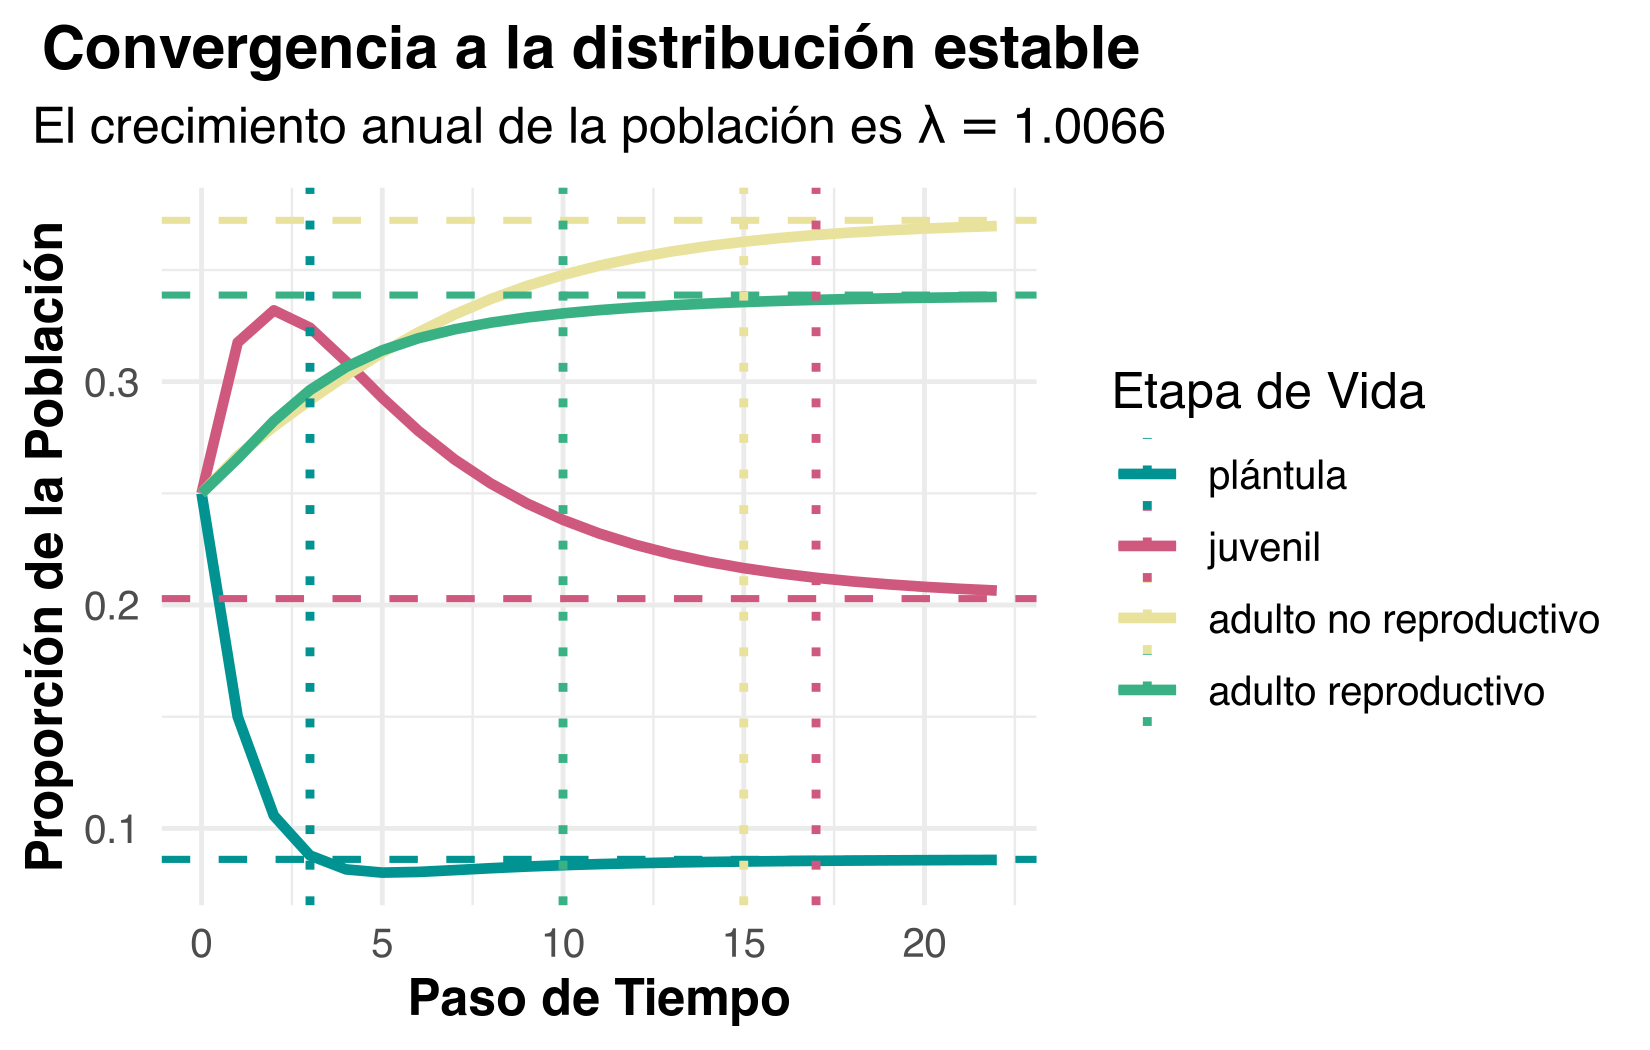
\includegraphics[keepaspectratio]{110-Propriedades_files/figure-pdf/indice16-1.png}}

Estas propiedades estructurales permiten comprender el significado
biológico de la tasa de crecimiento poblacional introducida en el
capítulo sobre crecimiento poblacional.

\bookmarksetup{startatroot}

\chapter{Elasticidad y Sensibilidad}\label{Elasticidad}

Autores: ``Demetria Mondragón, Ernesto Mujica y Elaine González''

La elasticidad poblacional permite identificar qué transiciones del
ciclo de vida tienen el mayor impacto proporcional sobre la tasa de
crecimiento poblacional (λ). Este capítulo introduce la lógica, el
cálculo y la interpretación aplicada de esta métrica.

\section{Elasticidad poblacional: porqué pequeñas variaciones
importan}\label{elasticidad-poblacional-porquuxe9-pequeuxf1as-variaciones-importan}

La elasticidad describe cuánto cambia la tasa de crecimiento poblacional
(λ) ante pequeñas variaciones proporcionales en los parámetros vitales
de la matriz (supervivencia, crecimiento, fecundidad). A diferencia de
la sensibilidad, que evalúa cambios absolutos, la elasticidad normaliza
por la magnitud del parámetro y permite comparar la influencia relativa
de transiciones con escalas distintas. En este módulo se muestra: (i)
cómo derivar elasticidades a partir del modelo matricial de
Leslie/Lefkovitch, (ii) por qué ciertas etapas (p.~ej., supervivencia en
adultos de larga vida) dominan λ, y (iii) cómo interpretar estos
resultados para priorizar acciones de manejo (protección de etapas
clave, reducción de variabilidad en tasas vitales críticas, etc.).
Incluimos ejemplos reproducibles con matrices reales y gráficos que
contrastan elasticidades vs.~sensibilidades, destacando cuándo la
decisión de manejo cambiaría si usamos una u otra métrica. Finalizamos
con recomendaciones prácticas: cómo reportar elasticidades con
intervalos de confianza, cómo evitar interpretaciones erróneas cuando
existen correlaciones entre transiciones, y cómo integrar elasticidades
en un análisis LTRE o en simulaciones de escenarios. Esta lección se
diferencia de las anteriores (fecundidad, crecimiento poblacional)
porque conecta directamente la teoría con decisiones de conservación,
mostrando el impacto marginal de cada transición sobre λ en términos
comparables y accionables.

\subsubsection{Librerías de R requeridas para el siguiente
módulo}\label{libreruxedas-de-r-requeridas-para-el-siguiente-muxf3dulo-8}

\begin{Shaded}
\begin{Highlighting}[]
\FunctionTok{library}\NormalTok{(popdemo)}
\FunctionTok{library}\NormalTok{(popbio)}
\FunctionTok{library}\NormalTok{(ggplot2)}
\FunctionTok{library}\NormalTok{(dplyr)}
\FunctionTok{library}\NormalTok{(scales)}
\FunctionTok{library}\NormalTok{(janitor)}
\FunctionTok{library}\NormalTok{(tidyr)}
\FunctionTok{library}\NormalTok{(flextable)}
\end{Highlighting}
\end{Shaded}

\begin{Shaded}
\begin{Highlighting}[]
\NormalTok{rlt\_theme }\OtherTok{\textless{}{-}} \FunctionTok{theme}\NormalTok{(}
  \AttributeTok{axis.title.y =} \FunctionTok{element\_text}\NormalTok{(}\AttributeTok{colour =} \StringTok{"grey20"}\NormalTok{, }\AttributeTok{size =} \DecValTok{10}\NormalTok{, }\AttributeTok{face =} \StringTok{"bold"}\NormalTok{),}
  \AttributeTok{axis.text.x =} \FunctionTok{element\_text}\NormalTok{(}\AttributeTok{colour =} \StringTok{"grey20"}\NormalTok{, }\AttributeTok{size =} \DecValTok{10}\NormalTok{, }\AttributeTok{face =} \StringTok{"bold"}\NormalTok{),}
  \AttributeTok{axis.text.y =} \FunctionTok{element\_text}\NormalTok{(}\AttributeTok{colour =} \StringTok{"grey20"}\NormalTok{, }\AttributeTok{size =} \DecValTok{15}\NormalTok{, }\AttributeTok{face =} \StringTok{"bold"}\NormalTok{),}
  \AttributeTok{axis.title.x =} \FunctionTok{element\_text}\NormalTok{(}\AttributeTok{colour =} \StringTok{"grey20"}\NormalTok{, }\AttributeTok{size =} \DecValTok{15}\NormalTok{, }\AttributeTok{face =} \StringTok{"bold"}\NormalTok{)}
\NormalTok{) }\SpecialCharTok{+}
  \FunctionTok{theme}\NormalTok{(}
    \CommentTok{\# Remover los bordes}
    \AttributeTok{panel.border =} \FunctionTok{element\_blank}\NormalTok{(),}
    \CommentTok{\# Remover las líneas}
    \AttributeTok{panel.grid.major =} \FunctionTok{element\_blank}\NormalTok{(),}
    \AttributeTok{panel.grid.minor =} \FunctionTok{element\_blank}\NormalTok{(),}
    \CommentTok{\# Remover el fondo del panel}
    \AttributeTok{panel.background =} \FunctionTok{element\_blank}\NormalTok{(),}
    \CommentTok{\# añadir lineas más gruesas}
    \AttributeTok{axis.line.x =} \FunctionTok{element\_line}\NormalTok{(}\AttributeTok{colour =} \StringTok{"black"}\NormalTok{, }\AttributeTok{linewidth =} \DecValTok{1}\NormalTok{),}
    \AttributeTok{axis.line.y =} \FunctionTok{element\_line}\NormalTok{(}\AttributeTok{colour =} \StringTok{"black"}\NormalTok{, }\AttributeTok{linewidth =} \DecValTok{1}\NormalTok{)}
\NormalTok{  )}

\NormalTok{diverging}\OtherTok{=} \FunctionTok{c}\NormalTok{(}\StringTok{"\#009392"}\NormalTok{,}\StringTok{"\#CF597E"}\NormalTok{,}\StringTok{"\#E9E29C"}\NormalTok{, }\StringTok{"\#39B185"}\NormalTok{,}\StringTok{"\#EEB479"}\NormalTok{ , }\StringTok{"\#9CCB86"}\NormalTok{ )}

\CommentTok{\# {-}{-}{-} 2. Combinarlos en un objeto de tipo lista {-}{-}{-}}
\CommentTok{\# Esta lista se puede añadir al gráfico con un solo \textquotesingle{}+\textquotesingle{}}
\NormalTok{rlt\_style\_fill }\OtherTok{\textless{}{-}} \ControlFlowTok{function}\NormalTok{() \{}
  \FunctionTok{list}\NormalTok{(}
\NormalTok{    rlt\_theme,}
    \FunctionTok{scale\_fill\_manual}\NormalTok{(}\AttributeTok{values =}\NormalTok{ diverging)}
\NormalTok{  )}
\NormalTok{\}}

\NormalTok{rlt\_style\_colour }\OtherTok{\textless{}{-}} \ControlFlowTok{function}\NormalTok{() \{ }\CommentTok{\#este es mi codigo personal de color}
  \FunctionTok{list}\NormalTok{(}
\NormalTok{    rlt\_theme,}
    \FunctionTok{scale\_colour\_manual}\NormalTok{(}\AttributeTok{values =}\NormalTok{ diverging)}
\NormalTok{  )}
\NormalTok{\}}
\end{Highlighting}
\end{Shaded}

\section{Qué es la elasticidad}\label{quuxe9-es-la-elasticidad}

Las matrices de elasticidad son un complemento de las matrices de
transición que nos permiten evaluar el efecto de pequeños cambios
proporcionales en los parámetros de la matriz sobre la tasa finita de
crecimiento poblacional (\(\lambda\)); las entradas de la matriz de
elasticidad con los valores más altos son las que más impacto tendrán
sobre el comportamiento de \(\lambda\) (Kroon et~al., 1986; Caswell,
2001). Para matrices no negativas, las elasticidades de las entradas
positivas son no negativas: aumentar \(a_{ij}\) incrementa (o no afecta)
a \(\lambda\), y disminuirla la reduce (o no la afecta) (Caswell, 2001).
El uso de las elasticidades en ecología de plantas se remonta a 1974,
cuando Sarukan y Gadgil intentaron evaluar la importancia relativa de la
reproducción sexual versus la reproducción vegetativa de tres especies
de \emph{Ranunculus} (Sarukhan \& Gadgil, 1974; Kroon et~al., 1986).

El concepto de elasticidad en biología es un método orientado a evaluar
el cambio proporcional en una variable en respuesta a un cambio
proporcional en otra variable. En términos de matrices de transición, la
elasticidad es una medida de la sensibilidad de la tasa de crecimiento
poblacional a los cambios en alguna de las entradas de la matriz. En
otras palabras, si uno cambia uno de los parámetros de la matriz de
transición, la elasticidad mide cuánto cambiaría la tasa de crecimiento
poblacional (Kroon et~al., 1986). En biología, la elasticidad es una
herramienta para entender la importancia \emph{del cambio} de cada etapa
de la historia de vida sobre la tasa de crecimiento poblacional, ya que
permite identificar las etapas que más contribuyen a la tasa de
crecimiento poblacional. Esta herramienta es muy útil para la
conservación de especies y para la gestión de recursos naturales, porque
en parte nos indica cuán sensible está el crecimiento poblacional cuando
se cambian los parámetros de la historia de vida (crecimiento,
supervivencia y fecundidad) de una especie. Un cambio proporcional se
refiere a que, por ejemplo, si se cambió el crecimiento en 1\%, qué
efecto tuvo sobre el crecimiento intrínseco de la población, versus si
se cambió el 1\% de la fertilidad. De esta forma uno tiene una
herramienta de comparación del impacto hipotético que tendrían los
cambios, en el caso de que se pudieran lograr.

Los valores de elasticidad en la Biología de la Conservación se pueden
interpretar como la vulnerabilidad de la población a perturbaciones en
cada transición. Formalmente, la elasticidad cuantifica el efecto
proporcional sobre \(\lambda\) de un cambio proporcional en una entrada
de la matriz, suponiendo equilibrio demográfico y perturbaciones
infinitesimales. Responde a la pregunta: ¿cuál de los cambios en las
tasas vitales, tomados de uno en uno y manteniendo los demás constantes,
produciría el mayor efecto sobre \(\lambda\)? En la práctica, las tasas
vitales con una baja elasticidad suelen tener una alta variabilidad
temporal, mientras que las de elevada elasticidad suelen variar poco ---
un patrón de canalización demográfica reportado tanto por Pfister como
por Ehrlén (Ehrlén \& Van Groenendael, 1998). Por ello no solo se debe
tener en cuenta cuán sensible es \(\lambda\) a una transición, sino
también cuánta variación en esa transición ocurre realmente y cómo
covaría con otras transiciones (Ehrlén \& Van Groenendael, 1998).

En términos matemáticos, la elasticidad es el cambio proporcional de
\(\lambda\) ante un cambio proporcional en una entrada de la matriz.
Concretamente, un cambio del 1\% en \(a_{ij}\) produce aproximadamente
\(e_{ij}\,\%\) de cambio en \(\lambda\) (válido para perturbaciones
infinitesimales) (Kroon et~al., 1986). La elasticidad \(e_{ij}\) de
\(\lambda\) con respecto a \(a_{ij}\) (la entrada \(i, j\) de la matriz)
se define como:

\[e_{ij}=\frac{a_{ij}}{\lambda}\,\frac{\partial \lambda}{\partial a_{ij}} = \frac{\partial \log \lambda}{\partial \log a_{ij}}\]

Es decir, \(e_{ij}\) es la pendiente de \(\log \lambda\) graficado
contra \(\log a_{ij}\). Como los incrementos en escala logarítmica
corresponden a cambios proporcionales en escala aritmética, la
elasticidad mide la sensibilidad \textbf{proporcional} (en contraste con
la sensibilidad absoluta \(\partial \lambda / \partial a_{ij}\)). Las
elasticidades pueden organizarse en una matriz de elasticidad
\(\mathbf{E}\) del mismo tamaño que la matriz de proyección:

\[\mathbf{E} = \frac{1}{\lambda}\,\mathbf{S} \circ \mathbf{A}\]

donde \(\mathbf{S}\) es la matriz de sensibilidad (con entradas
\(s_{ij} = \partial \lambda / \partial a_{ij}\)), \(\mathbf{A}\) es la
matriz de proyección y \(\circ\) es el producto de Hadamard
(multiplicación elemento por elemento) (Caswell, 2001). Aquí \(\lambda\)
es la \textbf{tasa finita de crecimiento} (per-unidad-de-tiempo); su
contraparte continua, la tasa intrínseca de incremento, es
\(r = \log \lambda\).

\begin{tcolorbox}[enhanced jigsaw, arc=.35mm, bottomrule=.15mm, bottomtitle=1mm, breakable, colback=white, colbacktitle=quarto-callout-note-color!10!white, colframe=quarto-callout-note-color-frame, coltitle=black, left=2mm, leftrule=.75mm, opacityback=0, opacitybacktitle=0.6, rightrule=.15mm, title=\textcolor{quarto-callout-note-color}{\faInfo}\hspace{0.5em}{Nota}, titlerule=0mm, toprule=.15mm, toptitle=1mm]

\textbf{Entradas de la matriz versus tasas vitales.} Las elasticidades
calculadas sobre \(a_{ij}\) son elasticidades de \textbf{entradas} de la
matriz, no de las tasas vitales subyacentes. Una entrada suele ser el
producto de varias tasas vitales: una transición \(a_{ij}\) típicamente
combina supervivencia × probabilidad de progreso de estadio, y una
entrada de fecundidad combina supervivencia × producción reproductiva
per cápita. Por tanto, la elasticidad de \(a_{ij}\) y la elasticidad de
cada tasa vital componente pueden diferir notablemente. Cuando una
decisión de manejo se basa en una sola tasa vital (p.~ej., supervivencia
adulta), conviene descomponer la entrada y calcular la elasticidad a
nivel de tasa vital (Franco \& Silvertown, 2004); ver también la sección
de \hyperref[limitaciones]{Limitaciones}.

\end{tcolorbox}

En contextos evolutivos, la elasticidad está estrechamente relacionada
con el \textbf{gradiente de selección} sobre los componentes de la
historia de vida: una entrada con alta elasticidad contribuye más a la
aptitud poblacional, y por tanto está sujeta a selección más fuerte
(Caswell, 1989a).

Las matrices de elasticidad tienen la ventaja de que la suma de las
entradas es igual a uno, por lo que permite sumar diferentes entradas de
la matriz, para evaluar la importancia de procesos (crecimiento,
decrecimiento, permanencia o reproducción) o de estadios (plántulas,
juveniles, adultos) sobre la \(\lambda\) (Silvertown, Franco \& Menges,
1996). Esta cualidad ha favorecido que matrices de elasticidad sean una
herramienta ampliamente utilizada para el desarrollo de planes de manejo
y conservación de especies, ya que permite identificar a que estadios
y/o procesos se deben enfocar los esfuerzos de conservación (Tremblay,
1997a; Mondragón, 2009; Berry \& Cleavitt, 2021; Timsina et~al., 2021) o
en caso opuesto para determinar que estadios pueden ser utilizados sin
impactar fuertemente a la población (Mondragón, 2009), es decir si
quisiéramos aprovechar una especie, de qué estadio tendríamos que
colectar, para impactar lo menos posible a la población.

\begin{center}\rule{0.5\linewidth}{0.5pt}\end{center}

\subsection{Sensibilidad y
elasticidad}\label{sensibilidad-y-elasticidad}

La diferencia entre sensibilidad y elasticidad es que la sensibilidad
mide el impacto en λ de cambiar la magnitud absoluta de una tasa vital
particular en relación con el cambio de otras tasas vitales (Caswell,
1989a), lo que implica que los cambios en las tasas de crecimiento y
permanencia tendrán un valor de uno (ya que se estas tasas son
proporciones), en tanto que los cambios en fecundidad podrán ser desde
uno hasta cientos o miles, ya que se la fecundidad se calcula con en
base a otra escala biológica (tal como número de semillas o plántulas).
La elasticidad por su parte calcula la sensibilidad proporcional de λ a
los cambios en una tasa vital (Kroon et~al., 1986) evitando de esta
forma el efecto de la magnitud del cambio. Cuanto mayor sea el valor de
la elasticidad de la tasa vital, mayor será la contribución relativa de
esa tasa vital al valor de lambda (\(\lambda\)).

\begin{center}\rule{0.5\linewidth}{0.5pt}\end{center}

\subsection{El impacto de cambio en las
etapas}\label{el-impacto-de-cambio-en-las-etapas}

Tomando como ejemplo la matriz de elasticidad de \emph{Erycina
crista-galli} una orquídea de ramilla (Mondragón, Maldonado \&
Aguilar-Santelises, 2007), podremos recapitular todo lo previamente
dicho (Tabla 1), así, lo \textbf{primero} que hay que recalcar es que el
valor más alto de elasticidad para esta orquídea corresponde a la
permanencia de los individuos adultos 2, es decir que cualquier pequeño
cambio en el valor de dicha entrada (en la matriz de transición), tendrá
el mayor impacto en el valor de lambda al comparar el valor de cambio en
dicho parámetro cuando se modifiquen otras entradas de la matriz;
\textbf{segundo}, es importante observar que al sumar todas las entradas
de la matriz se obtiene un valor de uno. Lo mismo se mantiene cuando se
suman todos los valores de elasticidad por estadio o por proceso. Es
decir, si sumamos todos los valores de cada columna, tendremos el valor
de elasticidad de cada estadio, para este caso el valor más alto lo
ostenta el de adultos 2 (0.818), lo que implica que el destino de la
población de \emph{E. crista-galli} depende mayormente de lo que les
pase a los individuos adultos.

\begin{Shaded}
\begin{Highlighting}[]
\NormalTok{etapas }\OtherTok{\textless{}{-}} \FunctionTok{c}\NormalTok{ (}\StringTok{"plántula"}\NormalTok{, }\StringTok{"juvenil"}\NormalTok{, }\StringTok{"adulto1"}\NormalTok{, }\StringTok{"adulto2"}\NormalTok{)}

\NormalTok{ec }\OtherTok{\textless{}{-}} \FunctionTok{matrix}\NormalTok{ (}\FunctionTok{c}\NormalTok{(}\DecValTok{0}\NormalTok{, }\DecValTok{0}\NormalTok{, }\FloatTok{0.004}\NormalTok{, }\FloatTok{0.062}\NormalTok{,}
                \FloatTok{0.195}\NormalTok{, }\DecValTok{0}\NormalTok{, }\DecValTok{0}\NormalTok{, }\DecValTok{0}\NormalTok{, }
                \FloatTok{0.171}\NormalTok{, }\FloatTok{0.120}\NormalTok{, }\FloatTok{0.053}\NormalTok{, }\FloatTok{0.04}\NormalTok{,}
                \FloatTok{0.073}\NormalTok{, }\FloatTok{0.10}\NormalTok{, }\FloatTok{0.435}\NormalTok{, }\FloatTok{0.447}\NormalTok{), }
      \AttributeTok{nrow =} \DecValTok{4}\NormalTok{, }\AttributeTok{ncol=}\DecValTok{4}\NormalTok{, }\AttributeTok{byrow =} \ConstantTok{TRUE}\NormalTok{, }
      \AttributeTok{dimnames =} \FunctionTok{list}\NormalTok{(etapas, etapas))}

\CommentTok{\# ec}
\end{Highlighting}
\end{Shaded}

\global\setlength{\Oldarrayrulewidth}{\arrayrulewidth}

\global\setlength{\Oldtabcolsep}{\tabcolsep}

\setlength{\tabcolsep}{2pt}

\renewcommand*{\arraystretch}{1.5}



\providecommand{\ascline}[3]{\noalign{\global\arrayrulewidth #1}\arrayrulecolor[HTML]{#2}\cline{#3}}

\begin{longtable*}[c]{ccccc}



\ascline{1.5pt}{666666}{1-5}

\multicolumn{1}{>{}l}{\textcolor[HTML]{000000}{\fontsize{11}{11}\selectfont{stages}}} & \multicolumn{1}{>{}r}{\textcolor[HTML]{000000}{\fontsize{11}{11}\selectfont{plántula}}} & \multicolumn{1}{>{}r}{\textcolor[HTML]{000000}{\fontsize{11}{11}\selectfont{juvenil}}} & \multicolumn{1}{>{}r}{\textcolor[HTML]{000000}{\fontsize{11}{11}\selectfont{adulto1}}} & \multicolumn{1}{>{}r}{\textcolor[HTML]{000000}{\fontsize{11}{11}\selectfont{adulto2}}} \\

\ascline{1.5pt}{666666}{1-5}\endfirsthead 

\ascline{1.5pt}{666666}{1-5}

\multicolumn{1}{>{}l}{\textcolor[HTML]{000000}{\fontsize{11}{11}\selectfont{stages}}} & \multicolumn{1}{>{}r}{\textcolor[HTML]{000000}{\fontsize{11}{11}\selectfont{plántula}}} & \multicolumn{1}{>{}r}{\textcolor[HTML]{000000}{\fontsize{11}{11}\selectfont{juvenil}}} & \multicolumn{1}{>{}r}{\textcolor[HTML]{000000}{\fontsize{11}{11}\selectfont{adulto1}}} & \multicolumn{1}{>{}r}{\textcolor[HTML]{000000}{\fontsize{11}{11}\selectfont{adulto2}}} \\

\ascline{1.5pt}{666666}{1-5}\endhead



\multicolumn{1}{>{}l}{\textcolor[HTML]{000000}{\fontsize{11}{11}\selectfont{plántula}}} & \multicolumn{1}{>{}r}{\textcolor[HTML]{000000}{\fontsize{11}{11}\selectfont{0.000}}} & \multicolumn{1}{>{}r}{\textcolor[HTML]{000000}{\fontsize{11}{11}\selectfont{0.000}}} & \multicolumn{1}{>{}r}{\textcolor[HTML]{000000}{\fontsize{11}{11}\selectfont{0.001}}} & \multicolumn{1}{>{}r}{\textcolor[HTML]{000000}{\fontsize{11}{11}\selectfont{0.058}}} \\





\multicolumn{1}{>{}l}{\textcolor[HTML]{000000}{\fontsize{11}{11}\selectfont{juvenil}}} & \multicolumn{1}{>{}r}{\textcolor[HTML]{000000}{\fontsize{11}{11}\selectfont{0.015}}} & \multicolumn{1}{>{}r}{\textcolor[HTML]{000000}{\fontsize{11}{11}\selectfont{0.000}}} & \multicolumn{1}{>{}r}{\textcolor[HTML]{000000}{\fontsize{11}{11}\selectfont{0.000}}} & \multicolumn{1}{>{}r}{\textcolor[HTML]{000000}{\fontsize{11}{11}\selectfont{0.000}}} \\





\multicolumn{1}{>{}l}{\textcolor[HTML]{000000}{\fontsize{11}{11}\selectfont{adulto1}}} & \multicolumn{1}{>{}r}{\textcolor[HTML]{000000}{\fontsize{11}{11}\selectfont{0.030}}} & \multicolumn{1}{>{}r}{\textcolor[HTML]{000000}{\fontsize{11}{11}\selectfont{0.008}}} & \multicolumn{1}{>{}r}{\textcolor[HTML]{000000}{\fontsize{11}{11}\selectfont{0.011}}} & \multicolumn{1}{>{}r}{\textcolor[HTML]{000000}{\fontsize{11}{11}\selectfont{0.059}}} \\





\multicolumn{1}{>{}l}{\textcolor[HTML]{000000}{\fontsize{11}{11}\selectfont{adulto2}}} & \multicolumn{1}{>{}r}{\textcolor[HTML]{000000}{\fontsize{11}{11}\selectfont{0.014}}} & \multicolumn{1}{>{}r}{\textcolor[HTML]{000000}{\fontsize{11}{11}\selectfont{0.007}}} & \multicolumn{1}{>{}r}{\textcolor[HTML]{000000}{\fontsize{11}{11}\selectfont{0.096}}} & \multicolumn{1}{>{}r}{\textcolor[HTML]{000000}{\fontsize{11}{11}\selectfont{0.702}}} \\





\multicolumn{1}{>{}l}{\textcolor[HTML]{000000}{\fontsize{11}{11}\selectfont{suma}}} & \multicolumn{1}{>{}r}{\textcolor[HTML]{000000}{\fontsize{11}{11}\selectfont{0.059}}} & \multicolumn{1}{>{}r}{\textcolor[HTML]{000000}{\fontsize{11}{11}\selectfont{0.015}}} & \multicolumn{1}{>{}r}{\textcolor[HTML]{000000}{\fontsize{11}{11}\selectfont{0.108}}} & \multicolumn{1}{>{}r}{\textcolor[HTML]{000000}{\fontsize{11}{11}\selectfont{0.819}}} \\

\ascline{1.5pt}{666666}{1-5}



\end{longtable*}



\arrayrulecolor[HTML]{000000}

\global\setlength{\arrayrulewidth}{\Oldarrayrulewidth}

\global\setlength{\tabcolsep}{\Oldtabcolsep}

\renewcommand*{\arraystretch}{1}

Tabla 1. Matriz de elasticidad de \emph{Erycina crista-galli}. En las
casillas del renglón ``suma'' se encuentra el resultado de la sumatoria
de los valores de elasticidad de cada entrada de la matriz por estadio
(es decir todos los valores de la columna).

\begin{center}\rule{0.5\linewidth}{0.5pt}\end{center}

\subsection{Cómo se calcula una elasticidad: mirar bajo el
capó}\label{cuxf3mo-se-calcula-una-elasticidad-mirar-bajo-el-capuxf3}

Los valores anteriores son producidos por \texttt{popbio::elas()}, que
internamente combina los autovectores derecho e izquierdo de la matriz
con el producto de Hadamard. Para ilustrar de dónde sale un valor de
elasticidad, podemos reconstruirlos paso a paso a partir de los
autovectores. La sensibilidad se obtiene de:

\[s_{ij} = \frac{v_i\, w_j}{\langle v, w \rangle}\]

donde \(w\) es el autovector derecho dominante (estructura estable de
estadios), \(v\) el autovector izquierdo dominante (valor reproductivo)
y \(\langle v, w \rangle = \sum_k v_k w_k\). La matriz de elasticidad se
obtiene como \(\mathbf{E} = (1/\lambda)\,\mathbf{S} \circ \mathbf{A}\)
(Caswell, 2001).

\begin{Shaded}
\begin{Highlighting}[]
\CommentTok{\# Paso 1: autovalor dominante y autovectores}
\NormalTok{ev }\OtherTok{\textless{}{-}} \FunctionTok{eigen}\NormalTok{(ec)}
\NormalTok{lambda }\OtherTok{\textless{}{-}} \FunctionTok{Re}\NormalTok{(ev}\SpecialCharTok{$}\NormalTok{values[}\DecValTok{1}\NormalTok{])              }\CommentTok{\# tasa finita de crecimiento (lambda)}
\NormalTok{w }\OtherTok{\textless{}{-}} \FunctionTok{Re}\NormalTok{(ev}\SpecialCharTok{$}\NormalTok{vectors[, }\DecValTok{1}\NormalTok{])                }\CommentTok{\# autovector derecho: estructura estable}

\NormalTok{ev\_t }\OtherTok{\textless{}{-}} \FunctionTok{eigen}\NormalTok{(}\FunctionTok{t}\NormalTok{(ec))}
\NormalTok{v }\OtherTok{\textless{}{-}} \FunctionTok{Re}\NormalTok{(ev\_t}\SpecialCharTok{$}\NormalTok{vectors[, }\DecValTok{1}\NormalTok{])              }\CommentTok{\# autovector izquierdo: valor reproductivo}

\CommentTok{\# Paso 2: matriz de sensibilidad S}
\NormalTok{S }\OtherTok{\textless{}{-}} \FunctionTok{outer}\NormalTok{(v, w) }\SpecialCharTok{/} \FunctionTok{sum}\NormalTok{(v }\SpecialCharTok{*}\NormalTok{ w)}

\CommentTok{\# Paso 3: matriz de elasticidad E = (1/lambda) * S o A}
\NormalTok{E\_manual }\OtherTok{\textless{}{-}}\NormalTok{ (S }\SpecialCharTok{*}\NormalTok{ ec) }\SpecialCharTok{/}\NormalTok{ lambda}
\FunctionTok{round}\NormalTok{(E\_manual, }\DecValTok{3}\NormalTok{)}
\end{Highlighting}
\end{Shaded}

\begin{verbatim}
         plántula juvenil adulto1 adulto2
plántula    0.000   0.000   0.001   0.058
juvenil     0.015   0.000   0.000   0.000
adulto1     0.030   0.008   0.011   0.059
adulto2     0.014   0.007   0.096   0.702
\end{verbatim}

\begin{Shaded}
\begin{Highlighting}[]
\CommentTok{\# Verificación: las entradas deben sumar a 1}
\FunctionTok{sum}\NormalTok{(E\_manual)}
\end{Highlighting}
\end{Shaded}

\begin{verbatim}
[1] 1
\end{verbatim}

El resultado coincide con la Tabla 1 (salvo redondeo) y la suma de todas
las entradas es 1, una propiedad fundamental de las matrices de
elasticidad para matrices no negativas y primitivas (Kroon et~al.,
1986).

\begin{center}\rule{0.5\linewidth}{0.5pt}\end{center}

\subsection{Efecto de cambio en las transiciones, crecimiento,
permanencia y de
fecundidad}\label{efecto-de-cambio-en-las-transiciones-crecimiento-permanencia-y-de-fecundidad}

En la tabla 2 se ven los diferentes valores de elasticidad por procesos
en \emph{Erycina crista-galli} (Mondragón, Maldonado \&
Aguilar-Santelises, 2007) y el impacto por diferentes procesos de la
historia de vida de la población. Ahora, si lo que quisiéramos saber es
que proceso o tasa vital es lo que rige el comportamiento de la
población, lo que se hace es sumar las entradas de la matriz que lo
representan, en este caso hemos puesto en diferentes colores las
entradas que manifiestan cada tasa, en rojo es la permanencia, en azul
el crecimiento, en amarillo el decrecimiento o retrogresión y en verde
la fecundidad. Eso nos permite determinar cuál es el impacto de
elasticidad por procesos y tasas vitales, sumando cada uno de los
valores en cada categoría. Es claro que el impacto principal para la
población de \emph{E. crista-galli} es la permanencia de los individuos,
seguido por el crecimiento, en tanto que la fecundidad y la retrogresión
tienen un impacto menor.

La suma de cada grupo:

\begin{itemize}
\tightlist
\item
  Permanencia: 0.713
\item
  Crecimiento: 0.170
\item
  Retrogresión: 0.060
\item
  Fecundidad: 0.058
\end{itemize}

\begin{Shaded}
\begin{Highlighting}[]
\CommentTok{\#elas(ec)}

\CommentTok{\# Convertir la matriz de elasticidad en un data frame}
\NormalTok{ec\_df }\OtherTok{=} \FunctionTok{as.data.frame}\NormalTok{(}\FunctionTok{elas}\NormalTok{(ec)) }\SpecialCharTok{|\textgreater{}} \FunctionTok{round}\NormalTok{(}\DecValTok{3}\NormalTok{)}

\CommentTok{\# Sumar las elasticidades por procesos (crecimiento, permanencia y fecundidad)}
\NormalTok{ec\_df}
\end{Highlighting}
\end{Shaded}

\begin{verbatim}
         plántula juvenil adulto1 adulto2
plántula    0.000   0.000   0.001   0.058
juvenil     0.015   0.000   0.000   0.000
adulto1     0.030   0.008   0.011   0.059
adulto2     0.014   0.007   0.096   0.702
\end{verbatim}

\begin{Shaded}
\begin{Highlighting}[]
\NormalTok{ec\_df }\SpecialCharTok{\%\textgreater{}\%}
  \FunctionTok{flextable}\NormalTok{()}
\end{Highlighting}
\end{Shaded}

\global\setlength{\Oldarrayrulewidth}{\arrayrulewidth}

\global\setlength{\Oldtabcolsep}{\tabcolsep}

\setlength{\tabcolsep}{2pt}

\renewcommand*{\arraystretch}{1.5}



\providecommand{\ascline}[3]{\noalign{\global\arrayrulewidth #1}\arrayrulecolor[HTML]{#2}\cline{#3}}

\begin{longtable*}[c]{cccc}



\ascline{1.5pt}{666666}{1-4}

\multicolumn{1}{>{}r}{\textcolor[HTML]{000000}{\fontsize{11}{11}\selectfont{plántula}}} & \multicolumn{1}{>{}r}{\textcolor[HTML]{000000}{\fontsize{11}{11}\selectfont{juvenil}}} & \multicolumn{1}{>{}r}{\textcolor[HTML]{000000}{\fontsize{11}{11}\selectfont{adulto1}}} & \multicolumn{1}{>{}r}{\textcolor[HTML]{000000}{\fontsize{11}{11}\selectfont{adulto2}}} \\

\ascline{1.5pt}{666666}{1-4}\endfirsthead 

\ascline{1.5pt}{666666}{1-4}

\multicolumn{1}{>{}r}{\textcolor[HTML]{000000}{\fontsize{11}{11}\selectfont{plántula}}} & \multicolumn{1}{>{}r}{\textcolor[HTML]{000000}{\fontsize{11}{11}\selectfont{juvenil}}} & \multicolumn{1}{>{}r}{\textcolor[HTML]{000000}{\fontsize{11}{11}\selectfont{adulto1}}} & \multicolumn{1}{>{}r}{\textcolor[HTML]{000000}{\fontsize{11}{11}\selectfont{adulto2}}} \\

\ascline{1.5pt}{666666}{1-4}\endhead



\multicolumn{1}{>{}r}{\textcolor[HTML]{000000}{\fontsize{11}{11}\selectfont{0.000}}} & \multicolumn{1}{>{}r}{\textcolor[HTML]{000000}{\fontsize{11}{11}\selectfont{0.000}}} & \multicolumn{1}{>{}r}{\textcolor[HTML]{000000}{\fontsize{11}{11}\selectfont{0.001}}} & \multicolumn{1}{>{}r}{\textcolor[HTML]{000000}{\fontsize{11}{11}\selectfont{0.058}}} \\





\multicolumn{1}{>{}r}{\textcolor[HTML]{000000}{\fontsize{11}{11}\selectfont{0.015}}} & \multicolumn{1}{>{}r}{\textcolor[HTML]{000000}{\fontsize{11}{11}\selectfont{0.000}}} & \multicolumn{1}{>{}r}{\textcolor[HTML]{000000}{\fontsize{11}{11}\selectfont{0.000}}} & \multicolumn{1}{>{}r}{\textcolor[HTML]{000000}{\fontsize{11}{11}\selectfont{0.000}}} \\





\multicolumn{1}{>{}r}{\textcolor[HTML]{000000}{\fontsize{11}{11}\selectfont{0.030}}} & \multicolumn{1}{>{}r}{\textcolor[HTML]{000000}{\fontsize{11}{11}\selectfont{0.008}}} & \multicolumn{1}{>{}r}{\textcolor[HTML]{000000}{\fontsize{11}{11}\selectfont{0.011}}} & \multicolumn{1}{>{}r}{\textcolor[HTML]{000000}{\fontsize{11}{11}\selectfont{0.059}}} \\





\multicolumn{1}{>{}r}{\textcolor[HTML]{000000}{\fontsize{11}{11}\selectfont{0.014}}} & \multicolumn{1}{>{}r}{\textcolor[HTML]{000000}{\fontsize{11}{11}\selectfont{0.007}}} & \multicolumn{1}{>{}r}{\textcolor[HTML]{000000}{\fontsize{11}{11}\selectfont{0.096}}} & \multicolumn{1}{>{}r}{\textcolor[HTML]{000000}{\fontsize{11}{11}\selectfont{0.702}}} \\

\ascline{1.5pt}{666666}{1-4}



\end{longtable*}



\arrayrulecolor[HTML]{000000}

\global\setlength{\arrayrulewidth}{\Oldarrayrulewidth}

\global\setlength{\tabcolsep}{\Oldtabcolsep}

\renewcommand*{\arraystretch}{1}

Tabla 2. Matriz de elasticidad de \emph{Erycina crista-galli}. Los
colores de las entradas de la matriz representan los procesos o tasas
vitales: rojo es la permanencia, azul el crecimiento, el amarillo el
decrecimiento o retrogresión y el verde la fecundidad. Así para obtener
el valor de elasticidad por proceso, se tendrían que sumar las entradas
de color que lo representen.

\begin{center}\rule{0.5\linewidth}{0.5pt}\end{center}

\subsection{¿Cómo se usan los análisis de elasticidad en un plan de
conservación?}\label{cuxf3mo-se-usan-los-anuxe1lisis-de-elasticidad-en-un-plan-de-conservaciuxf3n}

Por lo que, de manera simplista, pudiéramos decir que, si quisiéramos
desarrollar un plan de conservación para esta especie, nuestros
esfuerzos debieran enfocarse a asegurar la supervivencia de los
individuos adultos, ya la mortandad (por causas naturales o por cosecha)
de los individuos adultos tiene el mayor impacto sobre la persistencia
de la población. En tanto que si quisiéramos hacer un uso sustentable de
esta orquídea lo recomendable sería recolectar individuos juveniles,
cuyos valores de elasticidad son menores a la de los adultos. El impacto
de remover plántulas o juveniles de la población tendría menos impacto a
largo plazo sobre la supervivencia de la población.

\begin{tcolorbox}[enhanced jigsaw, arc=.35mm, bottomrule=.15mm, bottomtitle=1mm, breakable, colback=white, colbacktitle=quarto-callout-warning-color!10!white, colframe=quarto-callout-warning-color-frame, coltitle=black, left=2mm, leftrule=.75mm, opacityback=0, opacitybacktitle=0.6, rightrule=.15mm, title=\textcolor{quarto-callout-warning-color}{\faExclamationTriangle}\hspace{0.5em}{Advertencia}, titlerule=0mm, toprule=.15mm, toptitle=1mm]

\textbf{Importante:} estas conclusiones suponen perturbaciones pequeñas.
La elasticidad es una aproximación local que no captura efectos no
lineales, compensación demográfica ni dependencia de la densidad; por
ello no debe usarse para justificar cosechas sustanciales sin análisis
adicionales (ver §\hyperref[limitaciones]{Limitaciones} y el capítulo de
\href{113-Funciones_de_Transferencia.qmd}{funciones de transferencia}).

\end{tcolorbox}

\begin{center}\rule{0.5\linewidth}{0.5pt}\end{center}

\subsection{Comparación entre
especies}\label{comparaciuxf3n-entre-especies}

Las elasticidades también han sido utilizadas para establecer el
comportamiento demográfico de las especies, lo que ha permitido generar
patrones entre formas de vida, así como comparaciones tanto entre formas
de vida como entre especies (Silvertown, Franco \& Menges, 1996;
{Mondragón Chaparro et~al.}, 2015). Así, por ejemplo, si quisiéramos
comparar el comportamiento demográfico de las orquídeas de ramillas
versus las orquídeas epífitas convencionales (Tabla 3) (reconstruido de
(Mondragón, Maldonado \& Aguilar-Santelises, 2007)), veríamos que para
ambos tipos de orquídeas lo más importante es la permanencia
(supervivencia) de los individuos, en tanto que se puede observar una
diferencia entre la orquídea de ramilla y las otras, en la contribución
de los estadios al comportamiento de lambda, ya que para la primera, los
individuos reproductivos presentan mayores valores de elasticidad (al
igual que para \emph{Lepanthes eltoroensis}), en tanto que para las
otras orquídea los valores más altos de elasticidad los tienen los
individuos no reproductivos (Mondragón, Maldonado \& Aguilar-Santelises,
2007).

En la Figura 1 se observa los valores de elasticidad añadidos por
proceso de historia de vida para cinco especies de orquídeas epífitas:

\begin{figure}[H]

{\centering \pandocbounded{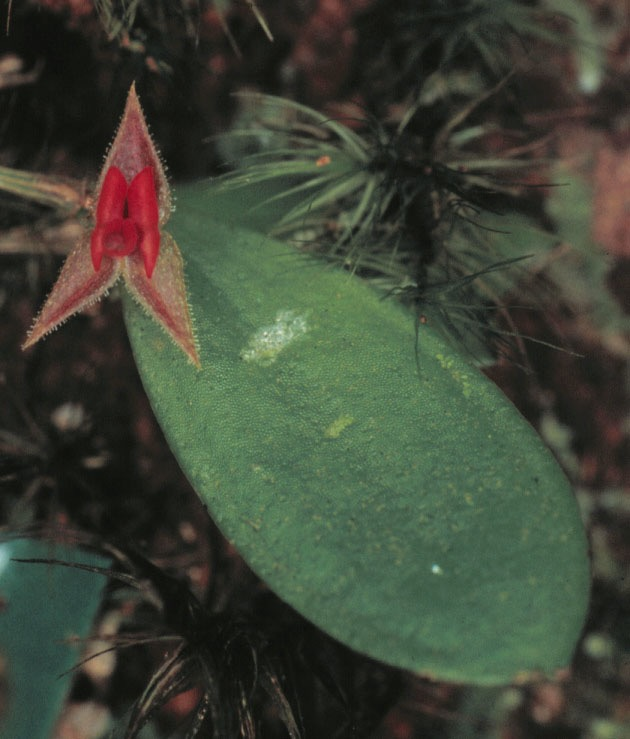
\includegraphics[keepaspectratio]{images/Lepanthes_eltoroensis_Tremblay.jpeg}}

}

\caption{\emph{Lepanthes eltoroensis}. Foto: Tremblay}

\end{figure}%

\begin{itemize}
\tightlist
\item
  \emph{Artorima erubescens} (Garcı́a-Soriano, 2003)
\item
  \emph{Erycina crista-galli} (Mondragón, Maldonado \&
  Aguilar-Santelises, 2007)
\item
  \emph{Laelia speciosa} (Hernández-Apolinar, 1992)
\item
  \emph{Lepanthes caritensis} (Tremblay, 1997a)
\item
  \emph{Lepanthes eltoroensis} (Tremblay \& Hutchings, 2003)
\end{itemize}

Se observa que los valores de elasticidad más altos corresponden a la
permanencia seguidos por el crecimiento.

Tabla 3. Valores elasticidad por proceso y por estadios no reproductivos
y reproductivos de cinco especies de orquídeas epífitas (\emph{Erycina
crista-galli}, considerada orquídea de ramilla).

\global\setlength{\Oldarrayrulewidth}{\arrayrulewidth}

\global\setlength{\Oldtabcolsep}{\tabcolsep}

\setlength{\tabcolsep}{2pt}

\renewcommand*{\arraystretch}{1.5}



\providecommand{\ascline}[3]{\noalign{\global\arrayrulewidth #1}\arrayrulecolor[HTML]{#2}\cline{#3}}

\begin{longtable*}[c]{ccccccc}



\ascline{1.5pt}{666666}{1-7}

\multicolumn{1}{>{}l}{\textcolor[HTML]{000000}{\fontsize{11}{11}\selectfont{Especie}}} & \multicolumn{1}{>{}r}{\textcolor[HTML]{000000}{\fontsize{11}{11}\selectfont{Fecundidad}}} & \multicolumn{1}{>{}r}{\textcolor[HTML]{000000}{\fontsize{11}{11}\selectfont{Estasis}}} & \multicolumn{1}{>{}r}{\textcolor[HTML]{000000}{\fontsize{11}{11}\selectfont{Crecimiento}}} & \multicolumn{1}{>{}r}{\textcolor[HTML]{000000}{\fontsize{11}{11}\selectfont{Plántulas}}} & \multicolumn{1}{>{}r}{\textcolor[HTML]{000000}{\fontsize{11}{11}\selectfont{No\_reproductivos}}} & \multicolumn{1}{>{}r}{\textcolor[HTML]{000000}{\fontsize{11}{11}\selectfont{Reproductivos}}} \\

\ascline{1.5pt}{666666}{1-7}\endfirsthead 

\ascline{1.5pt}{666666}{1-7}

\multicolumn{1}{>{}l}{\textcolor[HTML]{000000}{\fontsize{11}{11}\selectfont{Especie}}} & \multicolumn{1}{>{}r}{\textcolor[HTML]{000000}{\fontsize{11}{11}\selectfont{Fecundidad}}} & \multicolumn{1}{>{}r}{\textcolor[HTML]{000000}{\fontsize{11}{11}\selectfont{Estasis}}} & \multicolumn{1}{>{}r}{\textcolor[HTML]{000000}{\fontsize{11}{11}\selectfont{Crecimiento}}} & \multicolumn{1}{>{}r}{\textcolor[HTML]{000000}{\fontsize{11}{11}\selectfont{Plántulas}}} & \multicolumn{1}{>{}r}{\textcolor[HTML]{000000}{\fontsize{11}{11}\selectfont{No\_reproductivos}}} & \multicolumn{1}{>{}r}{\textcolor[HTML]{000000}{\fontsize{11}{11}\selectfont{Reproductivos}}} \\

\ascline{1.5pt}{666666}{1-7}\endhead



\multicolumn{1}{>{}l}{\textcolor[HTML]{000000}{\fontsize{11}{11}\selectfont{*Erycina\ crista-galli*}}} & \multicolumn{1}{>{}r}{\textcolor[HTML]{000000}{\fontsize{11}{11}\selectfont{0.035}}} & \multicolumn{1}{>{}r}{\textcolor[HTML]{000000}{\fontsize{11}{11}\selectfont{0.718}}} & \multicolumn{1}{>{}r}{\textcolor[HTML]{000000}{\fontsize{11}{11}\selectfont{0.247}}} & \multicolumn{1}{>{}r}{\textcolor[HTML]{000000}{\fontsize{11}{11}\selectfont{0.0345}}} & \multicolumn{1}{>{}r}{\textcolor[HTML]{000000}{\fontsize{11}{11}\selectfont{0.0456}}} & \multicolumn{1}{>{}r}{\textcolor[HTML]{000000}{\fontsize{11}{11}\selectfont{0.9197}}} \\





\multicolumn{1}{>{}l}{\textcolor[HTML]{000000}{\fontsize{11}{11}\selectfont{*Artorima\ erubescens*}}} & \multicolumn{1}{>{}r}{\textcolor[HTML]{000000}{\fontsize{11}{11}\selectfont{0.000}}} & \multicolumn{1}{>{}r}{\textcolor[HTML]{000000}{\fontsize{11}{11}\selectfont{0.646}}} & \multicolumn{1}{>{}r}{\textcolor[HTML]{000000}{\fontsize{11}{11}\selectfont{0.354}}} & \multicolumn{1}{>{}r}{\textcolor[HTML]{000000}{\fontsize{11}{11}\selectfont{0.0023}}} & \multicolumn{1}{>{}r}{\textcolor[HTML]{000000}{\fontsize{11}{11}\selectfont{0.7207}}} & \multicolumn{1}{>{}r}{\textcolor[HTML]{000000}{\fontsize{11}{11}\selectfont{0.2770}}} \\





\multicolumn{1}{>{}l}{\textcolor[HTML]{000000}{\fontsize{11}{11}\selectfont{*Laelia\ speciosa*}}} & \multicolumn{1}{>{}r}{\textcolor[HTML]{000000}{\fontsize{11}{11}\selectfont{0.116}}} & \multicolumn{1}{>{}r}{\textcolor[HTML]{000000}{\fontsize{11}{11}\selectfont{0.651}}} & \multicolumn{1}{>{}r}{\textcolor[HTML]{000000}{\fontsize{11}{11}\selectfont{0.328}}} & \multicolumn{1}{>{}r}{\textcolor[HTML]{000000}{\fontsize{11}{11}\selectfont{0.1200}}} & \multicolumn{1}{>{}r}{\textcolor[HTML]{000000}{\fontsize{11}{11}\selectfont{0.6690}}} & \multicolumn{1}{>{}r}{\textcolor[HTML]{000000}{\fontsize{11}{11}\selectfont{0.2160}}} \\





\multicolumn{1}{>{}l}{\textcolor[HTML]{000000}{\fontsize{11}{11}\selectfont{*Lepanthes\ eltoroensis*}}} & \multicolumn{1}{>{}r}{\textcolor[HTML]{000000}{\fontsize{11}{11}\selectfont{0.005}}} & \multicolumn{1}{>{}r}{\textcolor[HTML]{000000}{\fontsize{11}{11}\selectfont{0.880}}} & \multicolumn{1}{>{}r}{\textcolor[HTML]{000000}{\fontsize{11}{11}\selectfont{0.115}}} & \multicolumn{1}{>{}r}{\textcolor[HTML]{000000}{\fontsize{11}{11}\selectfont{0.1133}}} & \multicolumn{1}{>{}r}{\textcolor[HTML]{000000}{\fontsize{11}{11}\selectfont{0.0784}}} & \multicolumn{1}{>{}r}{\textcolor[HTML]{000000}{\fontsize{11}{11}\selectfont{0.8083}}} \\





\multicolumn{1}{>{}l}{\textcolor[HTML]{000000}{\fontsize{11}{11}\selectfont{*Lepanthes\ caritensis*}}} & \multicolumn{1}{>{}r}{\textcolor[HTML]{000000}{\fontsize{11}{11}\selectfont{0.002}}} & \multicolumn{1}{>{}r}{\textcolor[HTML]{000000}{\fontsize{11}{11}\selectfont{0.885}}} & \multicolumn{1}{>{}r}{\textcolor[HTML]{000000}{\fontsize{11}{11}\selectfont{0.114}}} & \multicolumn{1}{>{}r}{\textcolor[HTML]{000000}{\fontsize{11}{11}\selectfont{0.0180}}} & \multicolumn{1}{>{}r}{\textcolor[HTML]{000000}{\fontsize{11}{11}\selectfont{0.6480}}} & \multicolumn{1}{>{}r}{\textcolor[HTML]{000000}{\fontsize{11}{11}\selectfont{0.3350}}} \\

\ascline{1.5pt}{666666}{1-7}



\end{longtable*}



\arrayrulecolor[HTML]{000000}

\global\setlength{\arrayrulewidth}{\Oldarrayrulewidth}

\global\setlength{\tabcolsep}{\Oldtabcolsep}

\renewcommand*{\arraystretch}{1}

\begin{figure}[H]

{\centering \pandocbounded{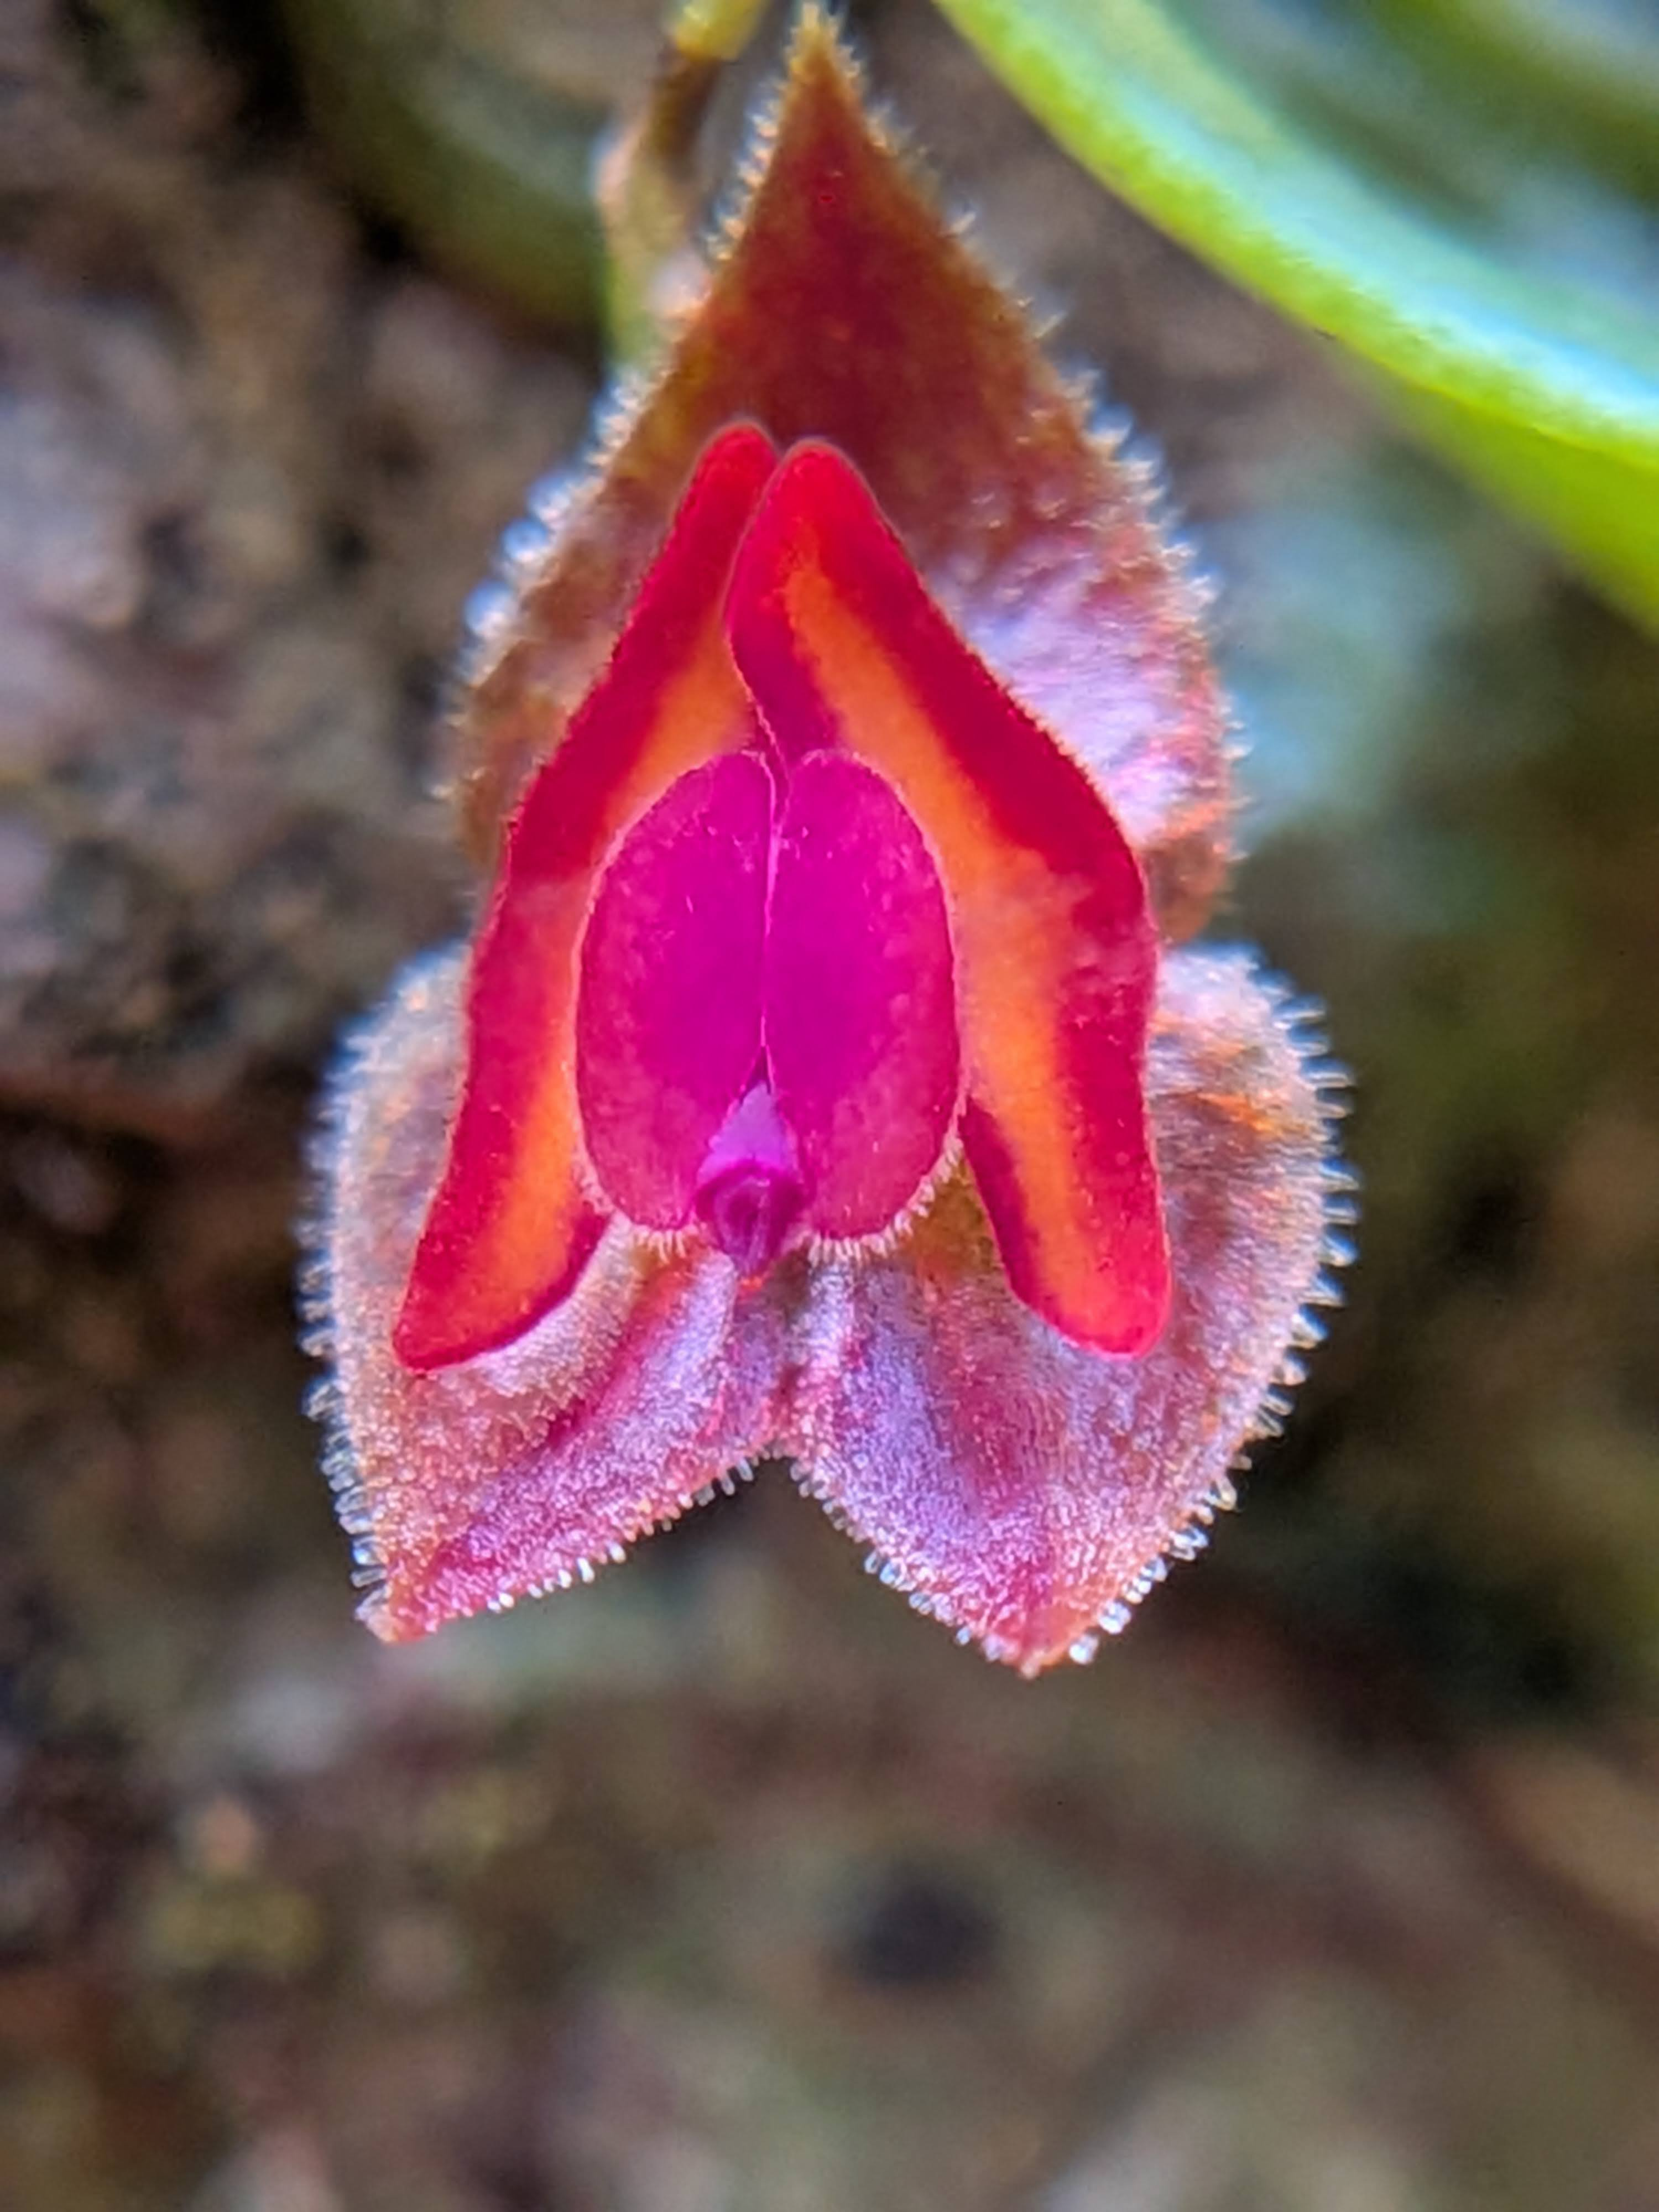
\includegraphics[keepaspectratio]{images/Lepanthes_caritensis_Edwin_Guevara.jpg}}

}

\caption{\emph{Lepanthes caritensis}. Foto: Edwin Guevara}

\end{figure}%

\begin{figure}[H]

{\centering \pandocbounded{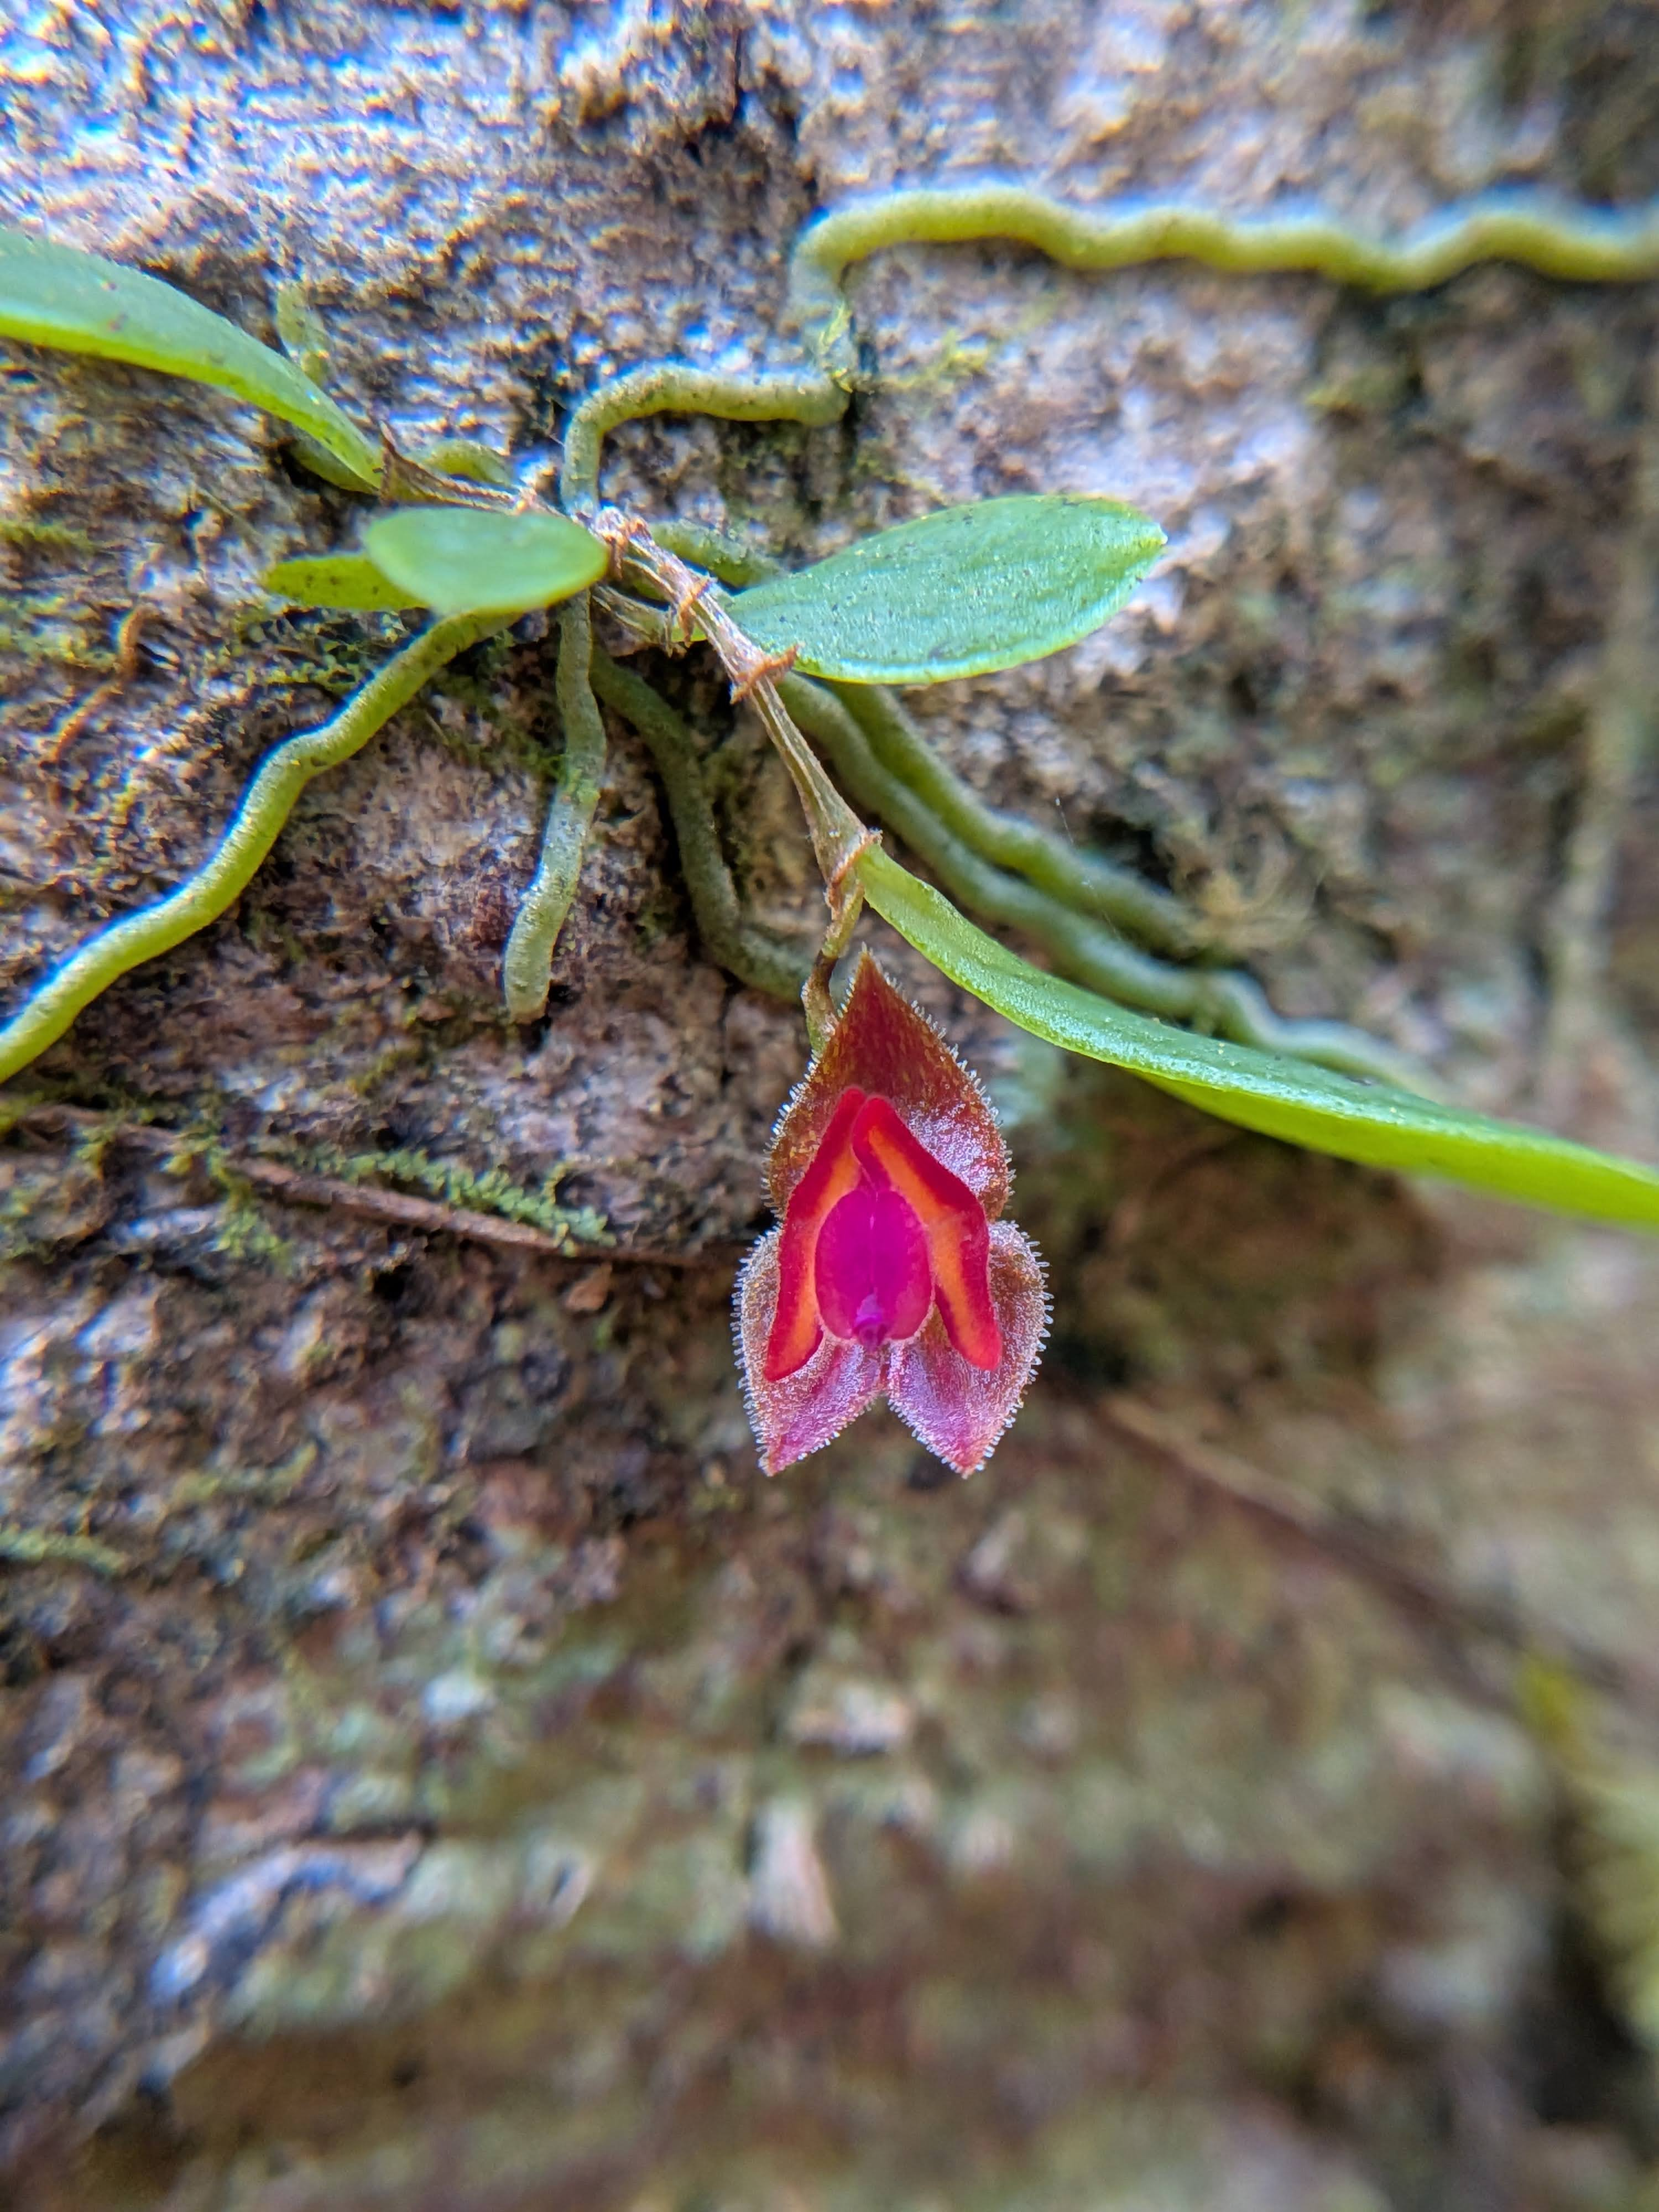
\includegraphics[keepaspectratio]{images/Lepanthes_caritensis_Phorophyte.jpg}}

}

\caption{\emph{Lepanthes caritensis}. Foto: Edwin Guevara}

\end{figure}%

\begin{Shaded}
\begin{Highlighting}[]
\NormalTok{EE }\OtherTok{=}\NormalTok{ Elasticidad\_s }\SpecialCharTok{\%\textgreater{}\%}
  \FunctionTok{select}\NormalTok{(Especie, Fecundidad, Estasis, Crecimiento) }\SpecialCharTok{\%\textgreater{}\%}
  \FunctionTok{pivot\_longer}\NormalTok{(}
    \AttributeTok{cols =} \SpecialCharTok{{-}}\NormalTok{Especie,}
    \AttributeTok{names\_to =} \StringTok{"s"}\NormalTok{,}
    \AttributeTok{values\_to =} \StringTok{"Elasticidad"}
\NormalTok{  )}

\NormalTok{EE}\SpecialCharTok{$}\NormalTok{s }\OtherTok{=} \FunctionTok{factor}\NormalTok{(}
\NormalTok{  EE}\SpecialCharTok{$}\NormalTok{s,}
  \AttributeTok{levels =} \FunctionTok{c}\NormalTok{(}\StringTok{"Fecundidad"}\NormalTok{, }\StringTok{"Estasis"}\NormalTok{, }\StringTok{"Crecimiento"}\NormalTok{)}
\NormalTok{)}

\FunctionTok{ggplot}\NormalTok{(EE, }\FunctionTok{aes}\NormalTok{(}\AttributeTok{x =}\NormalTok{ s, }\AttributeTok{y =}\NormalTok{ Elasticidad, }\AttributeTok{fill =}\NormalTok{ Especie)) }\SpecialCharTok{+}
  \FunctionTok{geom\_bar}\NormalTok{(}\AttributeTok{stat =} \StringTok{"identity"}\NormalTok{, }\AttributeTok{position =} \StringTok{"dodge"}\NormalTok{, }\AttributeTok{color =} \StringTok{"white"}\NormalTok{) }\SpecialCharTok{+}
  \FunctionTok{theme}\NormalTok{(}\AttributeTok{axis.text.x =} \FunctionTok{element\_text}\NormalTok{(}\AttributeTok{angle =} \DecValTok{45}\NormalTok{, }\AttributeTok{hjust =} \DecValTok{1}\NormalTok{)) }\SpecialCharTok{+}
  \FunctionTok{labs}\NormalTok{(}
    \AttributeTok{title =} \StringTok{"Elasticidad por proceso demográfico"}\NormalTok{,}
    \AttributeTok{x =} \StringTok{"s"}\NormalTok{,}
    \AttributeTok{y =} \StringTok{"Elasticidad"}
\NormalTok{  ) }\SpecialCharTok{+}
  \FunctionTok{scale\_fill\_discrete}\NormalTok{(}
    \AttributeTok{guide =} \FunctionTok{guide\_legend}\NormalTok{(}\AttributeTok{label.theme =} \FunctionTok{element\_text}\NormalTok{(}\AttributeTok{angle =} \DecValTok{0}\NormalTok{, }\AttributeTok{face =} \StringTok{"italic"}\NormalTok{))}
\NormalTok{  )}\SpecialCharTok{+}
  \FunctionTok{rlt\_style\_fill}\NormalTok{()}
\end{Highlighting}
\end{Shaded}

\pandocbounded{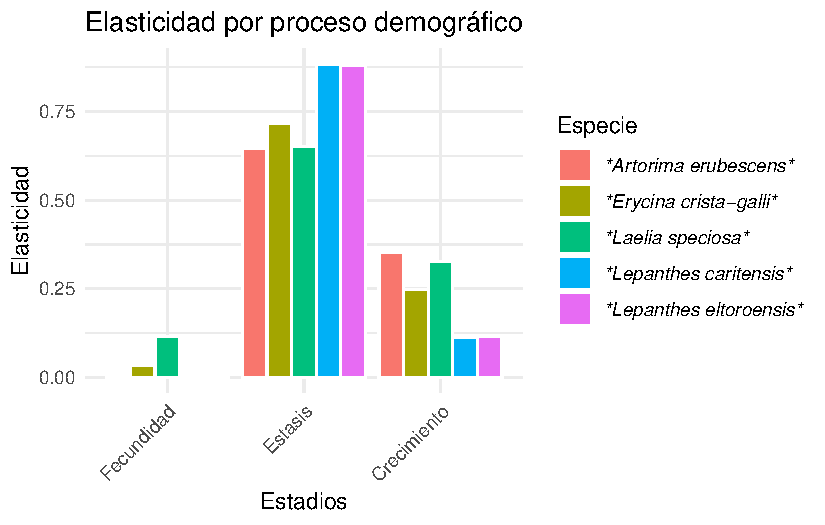
\includegraphics[keepaspectratio]{111-Elasticidad_files/figure-pdf/Elas7-1.pdf}}

Figura 1. Valores de elasticidad por proceso demográfico de cinco
especies de orquídeas epífitas.

En la figura 2 se observan los valores de elasticidad agrupados por
estadios (plántulas, individuos no reproductivos y reproductivos). Los
valores de elasticidad son más altos en los estadios no reproductivo en
tres especies y reproductivos (adultos activos) en dos especies. Las
plántulas tienen las elasticidad más pequeñas en todas las especies.

\begin{Shaded}
\begin{Highlighting}[]
\NormalTok{EE1 }\OtherTok{=}\NormalTok{ Elasticidad\_s }\SpecialCharTok{\%\textgreater{}\%}
  \FunctionTok{select}\NormalTok{(Especie, Plántulas, No\_reproductivos, Reproductivos) }\SpecialCharTok{\%\textgreater{}\%}
  \FunctionTok{pivot\_longer}\NormalTok{(}
    \AttributeTok{cols =} \SpecialCharTok{{-}}\NormalTok{Especie,}
    \AttributeTok{names\_to =} \StringTok{"s"}\NormalTok{,}
    \AttributeTok{values\_to =} \StringTok{"Elasticidad"}
\NormalTok{  )}

\NormalTok{EE1}\SpecialCharTok{$}\NormalTok{s2 }\OtherTok{=} \FunctionTok{factor}\NormalTok{(}
\NormalTok{  EE1}\SpecialCharTok{$}\NormalTok{s,}
  \AttributeTok{levels =} \FunctionTok{c}\NormalTok{(}\StringTok{"Plántulas"}\NormalTok{, }\StringTok{"No\_reproductivos"}\NormalTok{, }\StringTok{"Reproductivos"}\NormalTok{)}
\NormalTok{)}

\FunctionTok{ggplot}\NormalTok{(EE1, }\FunctionTok{aes}\NormalTok{(}\AttributeTok{x =}\NormalTok{ s2, }\AttributeTok{y =}\NormalTok{ Elasticidad, }\AttributeTok{fill =}\NormalTok{ Especie)) }\SpecialCharTok{+}
  \FunctionTok{geom\_bar}\NormalTok{(}\AttributeTok{stat =} \StringTok{"identity"}\NormalTok{, }\AttributeTok{position =} \StringTok{"dodge"}\NormalTok{, }\AttributeTok{color =} \StringTok{"white"}\NormalTok{) }\SpecialCharTok{+}
  \FunctionTok{theme}\NormalTok{(}\AttributeTok{axis.text.x =} \FunctionTok{element\_text}\NormalTok{(}\AttributeTok{angle =} \DecValTok{45}\NormalTok{, }\AttributeTok{hjust =} \DecValTok{1}\NormalTok{)) }\SpecialCharTok{+}
  \FunctionTok{labs}\NormalTok{(}
    \AttributeTok{title =} \StringTok{"Elasticidad por proceso demográfico"}\NormalTok{,}
    \AttributeTok{x =} \StringTok{"Etapas"}\NormalTok{,}
    \AttributeTok{y =} \StringTok{"Elasticidad"}
\NormalTok{  ) }\SpecialCharTok{+}
  \FunctionTok{scale\_fill\_discrete}\NormalTok{(}
    \AttributeTok{guide =} \FunctionTok{guide\_legend}\NormalTok{(}\AttributeTok{label.theme =} \FunctionTok{element\_text}\NormalTok{(}\AttributeTok{angle =} \DecValTok{0}\NormalTok{, }\AttributeTok{face =} \StringTok{"italic"}\NormalTok{))}
\NormalTok{  )}\SpecialCharTok{+}
  \FunctionTok{rlt\_style\_fill}\NormalTok{()}
\end{Highlighting}
\end{Shaded}

\pandocbounded{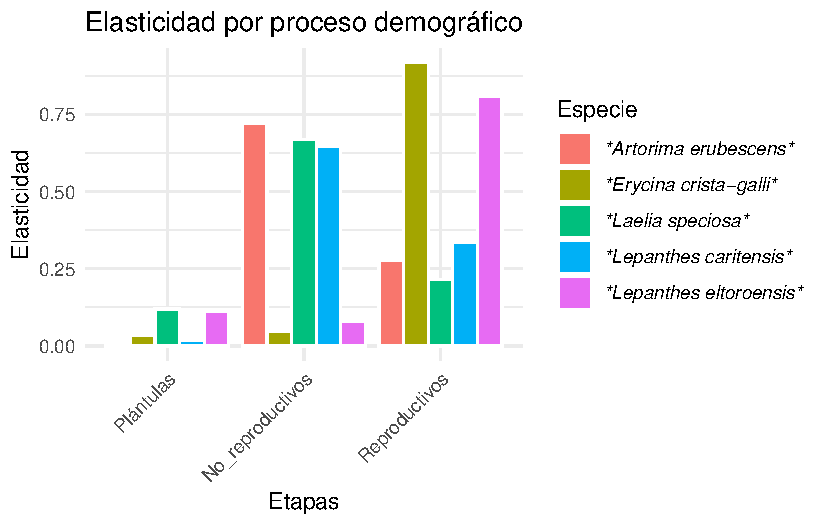
\includegraphics[keepaspectratio]{111-Elasticidad_files/figure-pdf/Elas8-1.pdf}}

Figura 2. Valores de elasticidad por estadio de cinco especies de
orquídeas epífitas.

\begin{center}\rule{0.5\linewidth}{0.5pt}\end{center}

\subsection{Elasticidad y LTRE: prospectivo versus
retrospectivo}\label{elasticidad-y-ltre-prospectivo-versus-retrospectivo}

La elasticidad es una herramienta \textbf{prospectiva}: pregunta qué
pasaría con \(\lambda\) si modificáramos hipotéticamente una entrada de
la matriz, manteniendo todo lo demás constante. Su contraparte natural
es el LTRE (\emph{Life Table Response Experiment}), una herramienta
\textbf{retrospectiva} que descompone diferencias \textbf{observadas} en
\(\lambda\) entre poblaciones, tratamientos o periodos en contribuciones
específicas de cada parámetro vital.

Las dos herramientas son complementarias: la elasticidad identifica las
transiciones donde un cambio tendría mayor impacto potencial, y el LTRE
cuantifica qué cambios efectivamente ocurrieron y cuánto contribuyeron
al cambio observado en \(\lambda\). Por ejemplo, una transición puede
tener alta elasticidad y, sin embargo, contribuir poco a una diferencia
observada entre años porque varía poco entre años; el LTRE permite
distinguir esto. Para la presentación formal del LTRE y un ejemplo
aplicado, ver el capítulo \hyperref[ERTV]{Experimento de Respuesta de
Tabla de Vida} (Caswell, 2001).

\begin{center}\rule{0.5\linewidth}{0.5pt}\end{center}

\begin{figure}[H]

{\centering \pandocbounded{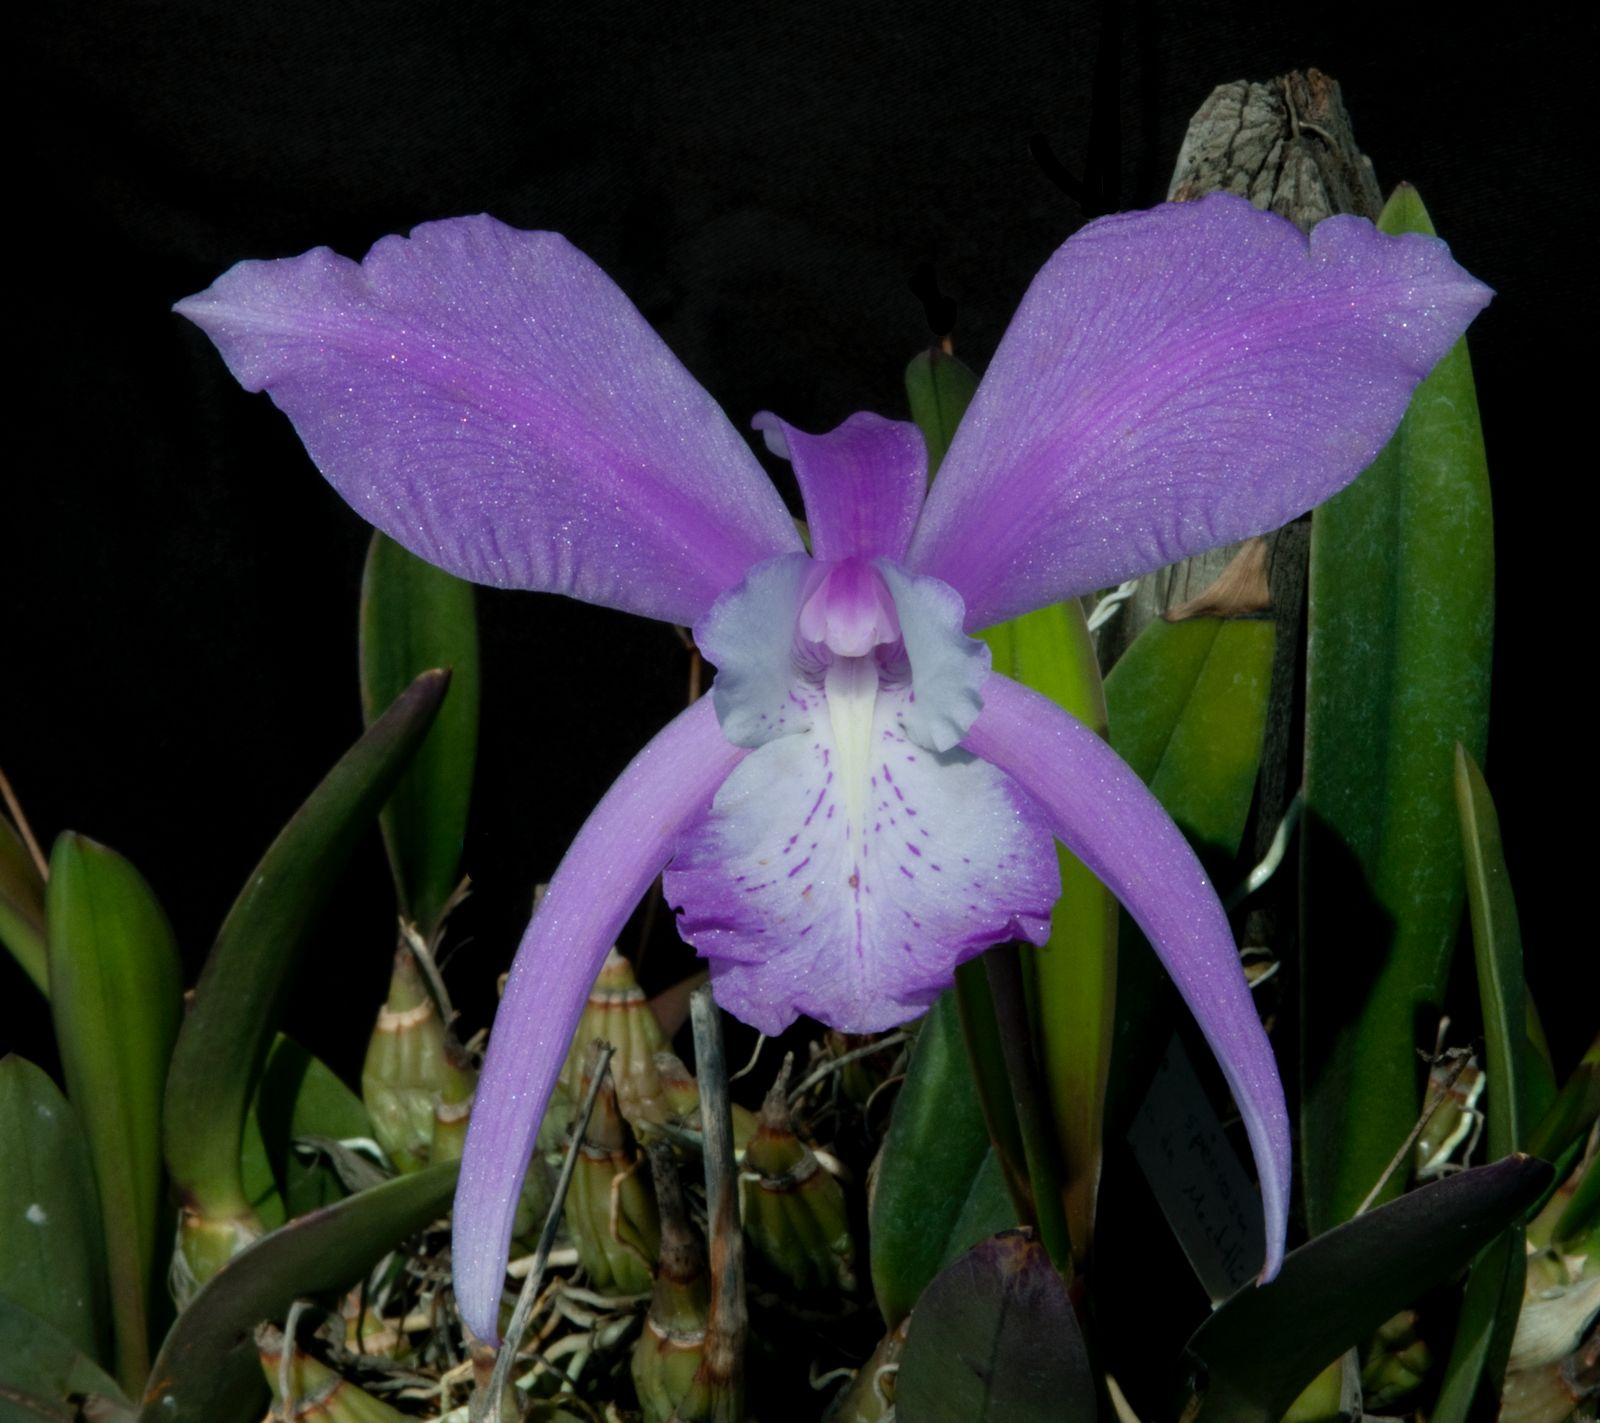
\includegraphics[keepaspectratio]{images/Laelia_speciosa_Eduardo_A._Perez_Garcia.jpeg}}

}

\caption{\emph{Laelia speciosa}. Foto: Eduardo A. Pérez García}

\end{figure}%

\section{Limitaciones}\label{limitaciones}

Aunque las matrices de elasticidad son una herramienta muy útil para
determinar el comportamiento demográfico de una especie o un conjunto de
estas, es necesario estar conscientes de que las diferentes entradas de
dichas matrices son el resultado, en la mayoría de los casos, de la
conjunción de varias tasas vitales a la vez (Franco \& Silvertown,
2004), además de que dependen fuertemente de la calidad de los datos.
Así mismo, es importante considerar que ciertas entradas son la
combinación de varios procesos demográficos. Por ejemplo, la entrada que
representa la transición de plántula a juvenil implica que el individuo
debe sobrevivir y además crecer lo suficiente para pasar al siguiente
estadio; o en el caso de la fecundidad, que el individuo debe sobrevivir
y además reproducirse. Por ello se recomienda separar los valores de
cada proceso de cada entrada y calcular las elasticidades de las tasas
vitales \emph{per se}. Por consecuencia, el acercamiento más reciente de
\emph{transient function} desarrollado por Stott et al. (Stott, Hodgson
\& Townley, 2012a) pudiese ser un acercamiento más adecuado si los
cambios son grandes, ya que muchos de los efectos no son lineales.
Adicionalmente, si la población está lejos de su estructura estable, la
elasticidad no es una buena aproximación de la respuesta de la población
a los cambios en las tasas vitales (Stott, Hodgson \& Townley, 2012a).
Por lo que es recomendable usar el análisis de elasticidad solamente
para poblaciones que están cerca de su equilibrio y cuando los cambios
en las tasas vitales son pequeños.

Una de las limitaciones principales del análisis de elasticidad
tradicional mencionado arriba es que el modelo de respuestas es lineal.
En otras palabras, se asume que los cambios en las tasas vitales son
proporcionales a los cambios en la tasa de crecimiento poblacional y
que, independientemente del tamaño del cambio, la respuesta seguirá un
patrón lineal. En la realidad, los cambios en las tasas vitales no son
proporcionales ni lineales a los cambios en la tasa de crecimiento
poblacional. Por ejemplo, si uno aumenta mucho la supervivencia de los
individuos de una etapa, la tasa de crecimiento poblacional no aumentará
de manera proporcional y lineal. Por consecuencia, la elasticidad es una
aproximación y no una descripción exacta de la relación entre los
cambios en las tasas vitales y la tasa de crecimiento poblacional, y es
aplicable solamente a análisis de perturbaciones pequeñas. Vea el
capítulo de funciones de transferencia para métodos más avanzados de
análisis de elasticidad.

Por último, las elasticidades calculadas mediante
\texttt{eigen.analysis()} o \texttt{popbio::elas()} son
\textbf{deterministas}: suponen un ambiente constante y una matriz fija.
Cuando las tasas vitales varían entre años por variabilidad ambiental,
conviene calcular \textbf{elasticidades estocásticas} sobre la tasa
estocástica de crecimiento \(\log \lambda_s\) (Caswell, 2001). Las
elasticidades estocásticas pueden diferir notablemente de las
deterministas, especialmente para tasas vitales con alta varianza
temporal, y son la métrica adecuada cuando el ambiente es marcadamente
variable. De forma análoga, dentro de un marco bayesiano la
incertidumbre en los parámetros vitales se propaga directamente a las
elasticidades, produciendo distribuciones posteriores en lugar de
valores puntuales (ver el capítulo
\hyperref[acercamiento-bayesiano-para-calcular-transiciones-y-fecundidades]{Acercamiento
bayesiano para calcular transiciones y fecundidades}).

\begin{center}\rule{0.5\linewidth}{0.5pt}\end{center}

\section{Resumen corto de los pasos}\label{resumen-corto-de-los-pasos}

\subsection{Introducir los nombres de los estadios o categorías de
tamaño según sea su
caso}\label{introducir-los-nombres-de-los-estadios-o-categoruxedas-de-tamauxf1o-seguxfan-sea-su-caso}

\begin{Shaded}
\begin{Highlighting}[]
\NormalTok{etapas }\OtherTok{\textless{}{-}} \FunctionTok{c}\NormalTok{ (}\StringTok{"plántula"}\NormalTok{, }\StringTok{"juvenil"}\NormalTok{, }\StringTok{"adulto1"}\NormalTok{, }\StringTok{"adulto2"}\NormalTok{)}
\end{Highlighting}
\end{Shaded}

\subsection{Capturar una matriz}\label{capturar-una-matriz}

Capturar los datos de la matriz para \emph{Erycina crita-galli}
(Mondragón, Maldonado \& Aguilar-Santelises, 2007) (tabla 4 dentro de
dicho artículo)

\begin{Shaded}
\begin{Highlighting}[]
\NormalTok{ec }\OtherTok{\textless{}{-}} \FunctionTok{matrix}\NormalTok{ (}\FunctionTok{c}\NormalTok{(}\DecValTok{0}\NormalTok{, }\DecValTok{0}\NormalTok{, }\FloatTok{0.004}\NormalTok{, }\FloatTok{0.062}\NormalTok{,}
                \FloatTok{0.195}\NormalTok{, }\DecValTok{0}\NormalTok{, }\DecValTok{0}\NormalTok{, }\DecValTok{0}\NormalTok{, }
                \FloatTok{0.171}\NormalTok{, }\FloatTok{0.120}\NormalTok{, }\FloatTok{0.053}\NormalTok{, }\FloatTok{0.04}\NormalTok{,}
                \FloatTok{0.073}\NormalTok{, }\FloatTok{0.10}\NormalTok{, }\FloatTok{0.435}\NormalTok{, }\FloatTok{0.447}\NormalTok{), }
      \AttributeTok{nrow =} \DecValTok{4}\NormalTok{, }\AttributeTok{ncol=}\DecValTok{4}\NormalTok{, }\AttributeTok{byrow =} \ConstantTok{TRUE}\NormalTok{, }
      \AttributeTok{dimnames =} \FunctionTok{list}\NormalTok{(etapas, etapas))}

\NormalTok{ec}
\end{Highlighting}
\end{Shaded}

\begin{verbatim}
         plántula juvenil adulto1 adulto2
plántula    0.000    0.00   0.004   0.062
juvenil     0.195    0.00   0.000   0.000
adulto1     0.171    0.12   0.053   0.040
adulto2     0.073    0.10   0.435   0.447
\end{verbatim}

\subsection{Valores iniciales de la
población}\label{valores-iniciales-de-la-poblaciuxf3n}

Introducir los valores iniciales por estadio (vector N): Cuantos
individuos hay en cada estadio al inicio del análisis.

\begin{Shaded}
\begin{Highlighting}[]
\NormalTok{N0\_ec }\OtherTok{\textless{}{-}} \FunctionTok{matrix}\NormalTok{(}\FunctionTok{c}\NormalTok{(}\DecValTok{41}\NormalTok{, }\DecValTok{50}\NormalTok{, }\DecValTok{246}\NormalTok{, }\DecValTok{226}\NormalTok{), }\AttributeTok{ncol =} \DecValTok{1}\NormalTok{)}

\NormalTok{N0\_ec}
\end{Highlighting}
\end{Shaded}

\begin{verbatim}
     [,1]
[1,]   41
[2,]   50
[3,]  246
[4,]  226
\end{verbatim}

\section{\texorpdfstring{La función
\texttt{eigen.analysis}}{La función eigen.analysis}}\label{la-funciuxf3n-eigen.analysis}

Para calcular los autovalores y autovectores de la matriz se usa la
función \texttt{eigen.analysis} del paquete \texttt{popbio}. Se obtiene
el crecimiento intrínseco \textbf{Lambda}, la sensibilidad, elasticidad,
valor reproductivo y \emph{damping ratio}. En el capítulo de propiedades
se presenta la interpretación de los valores reproductivos y el
\emph{damping ratio}.

\begin{Shaded}
\begin{Highlighting}[]
\FunctionTok{eigen.analysis}\NormalTok{(ec, }\AttributeTok{zero =} \ConstantTok{FALSE}\NormalTok{) }\CommentTok{\# la función es del paquete popbio}
\end{Highlighting}
\end{Shaded}

\begin{verbatim}
$lambda1
[1] 0.5214416

$stable.stage
  plántula    juvenil    adulto1    adulto2 
0.09190164 0.03436784 0.10775779 0.76597273 

$sensitivities
           plántula    juvenil   adulto1   adulto2
plántula 0.05877008 0.02197785 0.0689099 0.4898310
juvenil  0.03994690 0.01493867 0.0468391 0.3329455
adulto1  0.09172220 0.03430073 0.1075474 0.7644772
adulto2  0.09823314 0.03673558 0.1151817 0.8187439

$elasticities
           plántula     juvenil      adulto1    adulto2
plántula 0.00000000 0.000000000 0.0005286107 0.05824146
juvenil  0.01493867 0.000000000 0.0000000000 0.00000000
adulto1  0.03007910 0.007893670 0.0109312556 0.05864336
adulto2  0.01375230 0.007045004 0.0960875206 0.70185904

$repro.value
 plántula   juvenil   adulto1   adulto2 
1.0000000 0.6797151 1.5606957 1.6714823 

$damping.ratio
[1] 4.222528
\end{verbatim}

\section{Para seguir explorando}\label{para-seguir-explorando}

Tres direcciones complementarias profundizan los temas de este capítulo:

\begin{itemize}
\tightlist
\item
  \textbf{Análisis retrospectivo:} ver el capítulo
  \hyperref[ERTV]{Experimento de Respuesta de Tabla de Vida} para la
  descomposición de diferencias observadas en \(\lambda\) entre
  poblaciones, tratamientos o años.
\item
  \textbf{Perturbaciones grandes y dinámica transitoria:} ver el
  capítulo de \href{113-Funciones_de_Transferencia.qmd}{funciones de
  transferencia}, donde se relajan los supuestos de perturbaciones
  pequeñas y de equilibrio demográfico.
\item
  \textbf{Propagación explícita de la incertidumbre:} ver el capítulo de
  \hyperref[acercamiento-bayesiano-para-calcular-transiciones-y-fecundidades]{Acercamiento
  bayesiano para calcular transiciones y fecundidades}, donde las
  elasticidades se obtienen como distribuciones posteriores en lugar de
  valores puntuales.
\end{itemize}

\bookmarksetup{startatroot}

\chapter{Dinámica transitoria}\label{Dinamica_transitoria}

La dinámica de transiciones describe cómo los procesos demográficos
cambian a través del tiempo y del contexto ambiental. Este capítulo
introduce la variación temporal de las transiciones como un componente
clave para entender poblaciones que no se comportan de manera
estacionaria.

Por: Mariana Hernández-Apolinar, Tamara Ticktin y Paola Portillo Tzompa

\section{Variación temporal de las transiciones
demográficas}\label{variaciuxf3n-temporal-de-las-transiciones-demogruxe1ficas}

En los modelos básicos de dinámica poblacional, las transiciones entre
estadios suelen asumirse constantes en el tiempo. Sin embargo, en
sistemas reales, las tasas de supervivencia, crecimiento y fecundidad
pueden variar entre años, estaciones o en respuesta a condiciones
ambientales y perturbaciones externas. La dinámica de transiciones
aborda explícitamente esta variabilidad temporal como un proceso central
de la dinámica poblacional.

En este capítulo se exploran los fundamentos conceptuales para modelar
transiciones que cambian en el tiempo, mostrando cómo esta variación
influye en la trayectoria poblacional y en la interpretación de
parámetros como la tasa de crecimiento poblacional. Se discuten
distintas fuentes de variación temporal, incluyendo fluctuaciones
ambientales, densodependencia y respuestas a eventos extremos, así como
los supuestos asociados a su representación en modelos poblacionales.

A diferencia de los capítulos sobre transiciones demográficas estáticas
o descomposición matricial, este capítulo se centra en la
\textbf{dinámica temporal} de los procesos demográficos. Comprender cómo
y por qué cambian las transiciones en el tiempo resulta esencial para
interpretar resultados de simulaciones poblacionales, analizar
respuestas a escenarios de manejo y evaluar la estabilidad o
vulnerabilidad de las poblaciones frente a variabilidad ambiental. Este
enfoque proporciona el vínculo conceptual entre los modelos
estructurados clásicos y enfoques dinámicos más realistas.

\section{Modelación de transiciones variables en el
tiempo}\label{modelaciuxf3n-de-transiciones-variables-en-el-tiempo}

A continuación se presentan los enfoques utilizados para representar
transiciones demográficas que cambian en el tiempo, incluyendo
formulaciones determinísticas y dependientes de covariables. La
variación temporal de las transiciones puede representarse mediante
secuencias de matrices \textbf{U} y \textbf{F}, descritas en el capítulo
sobre matrices U, F y C.

\subsubsection{Librerías de R requeridas para el siguiente
módulo}\label{libreruxedas-de-r-requeridas-para-el-siguiente-muxf3dulo-9}

\begin{Shaded}
\begin{Highlighting}[]
\DocumentationTok{\#\# Librerías de R requeridas para el análisis}

\FunctionTok{library}\NormalTok{(popdemo)}
\FunctionTok{library}\NormalTok{(popbio)}
\FunctionTok{library}\NormalTok{(ggplot2)}
\FunctionTok{library}\NormalTok{(dplyr)}
\FunctionTok{library}\NormalTok{(scales)}
\FunctionTok{library}\NormalTok{(tidyverse)}
\FunctionTok{library}\NormalTok{(flextable)}
\end{Highlighting}
\end{Shaded}

\section{Dinámica poblacional a largo y corto
plazo}\label{dinuxe1mica-poblacional-a-largo-y-corto-plazo}

Los modelos de proyección poblacional (MPP), previamente abordados en el
capítulo de
\hyperref[propiedades-de-las-matrices-y-estimaciuxf3n-de-paruxe1metros]{Propiedades
poblacionales}, constituyen las herramientas más empleadas para estimar
el crecimiento futuro de una población (i.e., largo plazo). Estos
modelos suelen asumir la constancia en las tasas vitales ---proporciones
de mortalidad, reproducción y crecimiento de los individuos en las
distintas categorías poblacionales--- bajo condiciones ambientales
invariables (Caswell, 2001; {Crone et~al.}, 2011; Koons, Iles \& Stott,
2021). En ausencia de variación (i.e., modelos deterministas), se espera
que la población crezca o decrezca a una velocidad constante, denominada
tasa finita o asintótica de crecimiento poblacional (\(λ\))
(Bierzychudek, 1999; Caswell, 2001). Este patrón estable se alcanza
cuando la proporción de individuos por categoría de tamaño o estado
permanece constante, condición conocida como estructura estable (\(w\)).

Sin embargo, en sistemas naturales las condiciones poblacionales y
ambientales rara vez son constantes. Las poblaciones enfrentan recursos
limitados (e.g., alimento, refugio), ambientes heterogéneos y
perturbaciones (e.g., deforestación, sequías, huracanes, enfermedades),
que alteran su dinámica y evidencian que la tasa de crecimiento a largo
plazo (\(λ\)) no siempre predice adecuadamente los cambios poblacionales
(Bierzychudek, 1999). Por ello, se han desarrollado modelos que
incorporan variabilidad ambiental y permiten proyecciones más realistas,
como los modelos estocásticos (ver el capítulo de
\hyperref[Crecimiento_Poblacional]{Crecimiento poblacional}) y los
análisis de dinámica transitoria.

\section{Modelos de dinámica
transitoria}\label{modelos-de-dinuxe1mica-transitoria}

Los modelos de dinámica transitoria se proponen como alternativa para
evaluar la respuesta poblacional ante perturbaciones súbitas de origen
biótico (e.g., depredación), abiótico (e.g., huracán) o antropogénico
(e.g., extracción) (Ezard et~al., 2010). Una característica distintiva
es que el disturbio afecta únicamente la estructura poblacional, sin
modificar los valores de la matriz de transición, que permanecen
constantes en el tiempo (Stott, Townley \& Hodgson, 2011; {Vindenes
et~al.}, 2021). Este cambio abrupto genera una respuesta instantánea,
temporal y a corto plazo, generalmente distinta a la dinámica esperada a
largo plazo (Ezard et~al., 2010; Stott et~al., 2010a; Koons, Iles \&
Stott, 2021).

Para comprender cómo la estructura inicial influye en el crecimiento
poblacional, estos modelos asumen una estructura inestable, lo que
permite analizar la respuesta antes de alcanzar el crecimiento
asintótico (i.e., \(λ\) constante y estructura estable) (Bierzychudek,
1999; Stott, Townley \& Hodgson, 2011; Stott, Hodgson \& Townley, 2012a;
Koons, Iles \& Stott, 2021). La respuesta se evalúa mediante las
discrepancias entre el comportamiento poblacional bajo una o varias
estructuras iniciales (corto plazo) y la estructura estable (largo
plazo) (Raventós et~al., 2015). Dichas diferencias se reflejan en
incrementos (ampliación), decrementos (atenuación) o fluctuaciones en la
abundancia poblacional a corto plazo respecto al largo plazo (Stott,
Townley \& Hodgson, 2011), cuantificadas mediante los índices de
transferencia (Stott, Townley \& Hodgson, 2011).

Actualmente, los modelos de dinámica transitoria han demostrado ser
herramientas valiosas en estudios poblacionales de orquídeas, ya que
permiten evaluar estrategias de conservación y manejo (Raventós et~al.,
2015; Tremblay, Raventos \& Ackerman, 2015; Ospina-Calderón et~al.,
2023). Aunque estos análisis existen desde hace décadas ({Crone et~al.},
2011), su accesibilidad aumentó significativamente a partir de 2010
(Stott, Hodgson \& Townley, 2012b).

\begin{tcolorbox}[enhanced jigsaw, arc=.35mm, bottomrule=.15mm, bottomtitle=1mm, breakable, colback=white, colbacktitle=quarto-callout-important-color!10!white, colframe=quarto-callout-important-color-frame, coltitle=black, left=2mm, leftrule=.75mm, opacityback=0, opacitybacktitle=0.6, rightrule=.15mm, title=\textcolor{quarto-callout-important-color}{\faExclamation}\hspace{0.5em}{Importante}, titlerule=0mm, toprule=.15mm, toptitle=1mm]

\textbf{λ y la dinámica transitoria responden a preguntas distintas.}

\begin{itemize}
\tightlist
\item
  \textbf{Asintótica (λ):} ¿qué pasaría con la población \textbf{a largo
  plazo} si las tasas vitales y la estructura de estadios se mantuvieran
  constantes? Indiferente a la estructura inicial.
\item
  \textbf{Transitoria:} ¿qué pasa con la población
  \textbf{inmediatamente después} de una perturbación, antes de que
  alcance la estructura estable? \textbf{Depende fuertemente} de la
  estructura inicial.
\end{itemize}

Una población con \(\lambda = 1.10\) no necesariamente crecerá un 10\%
el primer año: si su estructura está sesgada (todos plántulas, todos
adultos), puede inicialmente decrecer, oscilar o crecer mucho más rápido
que λ --- y sólo después de varios pasos de tiempo el comportamiento
converge al asintótico.

\end{tcolorbox}

El marco metodológico propuesto por Stott y colaboradores (Stott,
Townley \& Hodgson, 2011; Stott, Hodgson \& Townley, 2012b; Stott,
Hodgson \& Townley, 2012a) incluye procedimientos matemáticos
implementados en el software estadístico R, que facilitan el cálculo y
análisis de la dinámica transitoria. Para desarrollar un proyecto de
este tipo, se recomienda seguir los pasos resumidos a continuación:

\subsection{Procedimiento básico}\label{procedimiento-buxe1sico}

\begin{enumerate}
\def\labelenumi{\arabic{enumi})}
\tightlist
\item
  \textbf{Análisis de la dinámica a largo plazo}
\end{enumerate}

\begin{itemize}
\tightlist
\item
  Construcción de la matriz de transición y definición de la estructura
  inicial.
\item
  Estimación del crecimiento asintótico (\(λ\)).
\end{itemize}

\begin{enumerate}
\def\labelenumi{\arabic{enumi})}
\setcounter{enumi}{1}
\tightlist
\item
  \textbf{Análisis de la dinámica a corto plazo}
\end{enumerate}

\begin{itemize}
\tightlist
\item
  Definición de la estructura poblacional inicial.
\item
  Evaluación de la dinámica absoluta.
\item
  Dinámica transitoria estandarizada.
\item
  Cálculo de límites transitorios.
\end{itemize}

Cabe destacar que los modelos de dinámica transitoria constituyen la
única herramienta para evaluar poblaciones que nunca convergen ---o cuya
convergencia es improbable--- hacia una estructura estable (Hinrichsen,
2025).

\begin{center}\rule{0.5\linewidth}{0.5pt}\end{center}

\section{Proyecto de dinámica transitoria o a corto
plazo}\label{proyecto-de-dinuxe1mica-transitoria-o-a-corto-plazo}

\subsection{Análisis de la dinámica a largo
plazo}\label{anuxe1lisis-de-la-dinuxe1mica-a-largo-plazo}

Como punto de partida y con la finalidad de contrastar su comportamiento
con la dinámica a corto plazo, se describe el crecimiento de la
población a largo plazo: tasas vitales constantes y en condiciones
ambientales sin variación. Con este objetivo, se requiere contar con la
matriz de transición y la estructura poblacional inicial para,
finalmente, estimar la tasa de crecimiento a largo plazo.

\begin{enumerate}
\def\labelenumi{\alph{enumi})}
\tightlist
\item
  \emph{Matriz de transición y estructura poblacional inicial}. Para
  estimar el crecimiento futuro de la población se debe de contar con la
  matriz de proyección poblacional y su correspondiente vector de la
  estructura poblacional observada al inicio del estudio de una o varias
  poblaciones. En el análisis se usarán los datos obtenidos para
  \emph{Lepanthes rubripetala}, una orquídea epífita miniatura, endémica
  de Puerto Rico. Tremblay y colaboradores (Tremblay, Raventos \&
  Ackerman, 2015) analizaron mensualmente seis poblaciones de la especie
  de junio de 1994 a enero de 1996. En específico en este capítulo
  usaremos la matriz promedio de la población 1 (Tremblay, Raventos \&
  Ackerman, 2015) y su correspondiente estructura poblacional
  (Schödelbauerová, Tremblay \& Kindlmann, 2010).
\end{enumerate}

\begin{figure}[H]

{\centering \pandocbounded{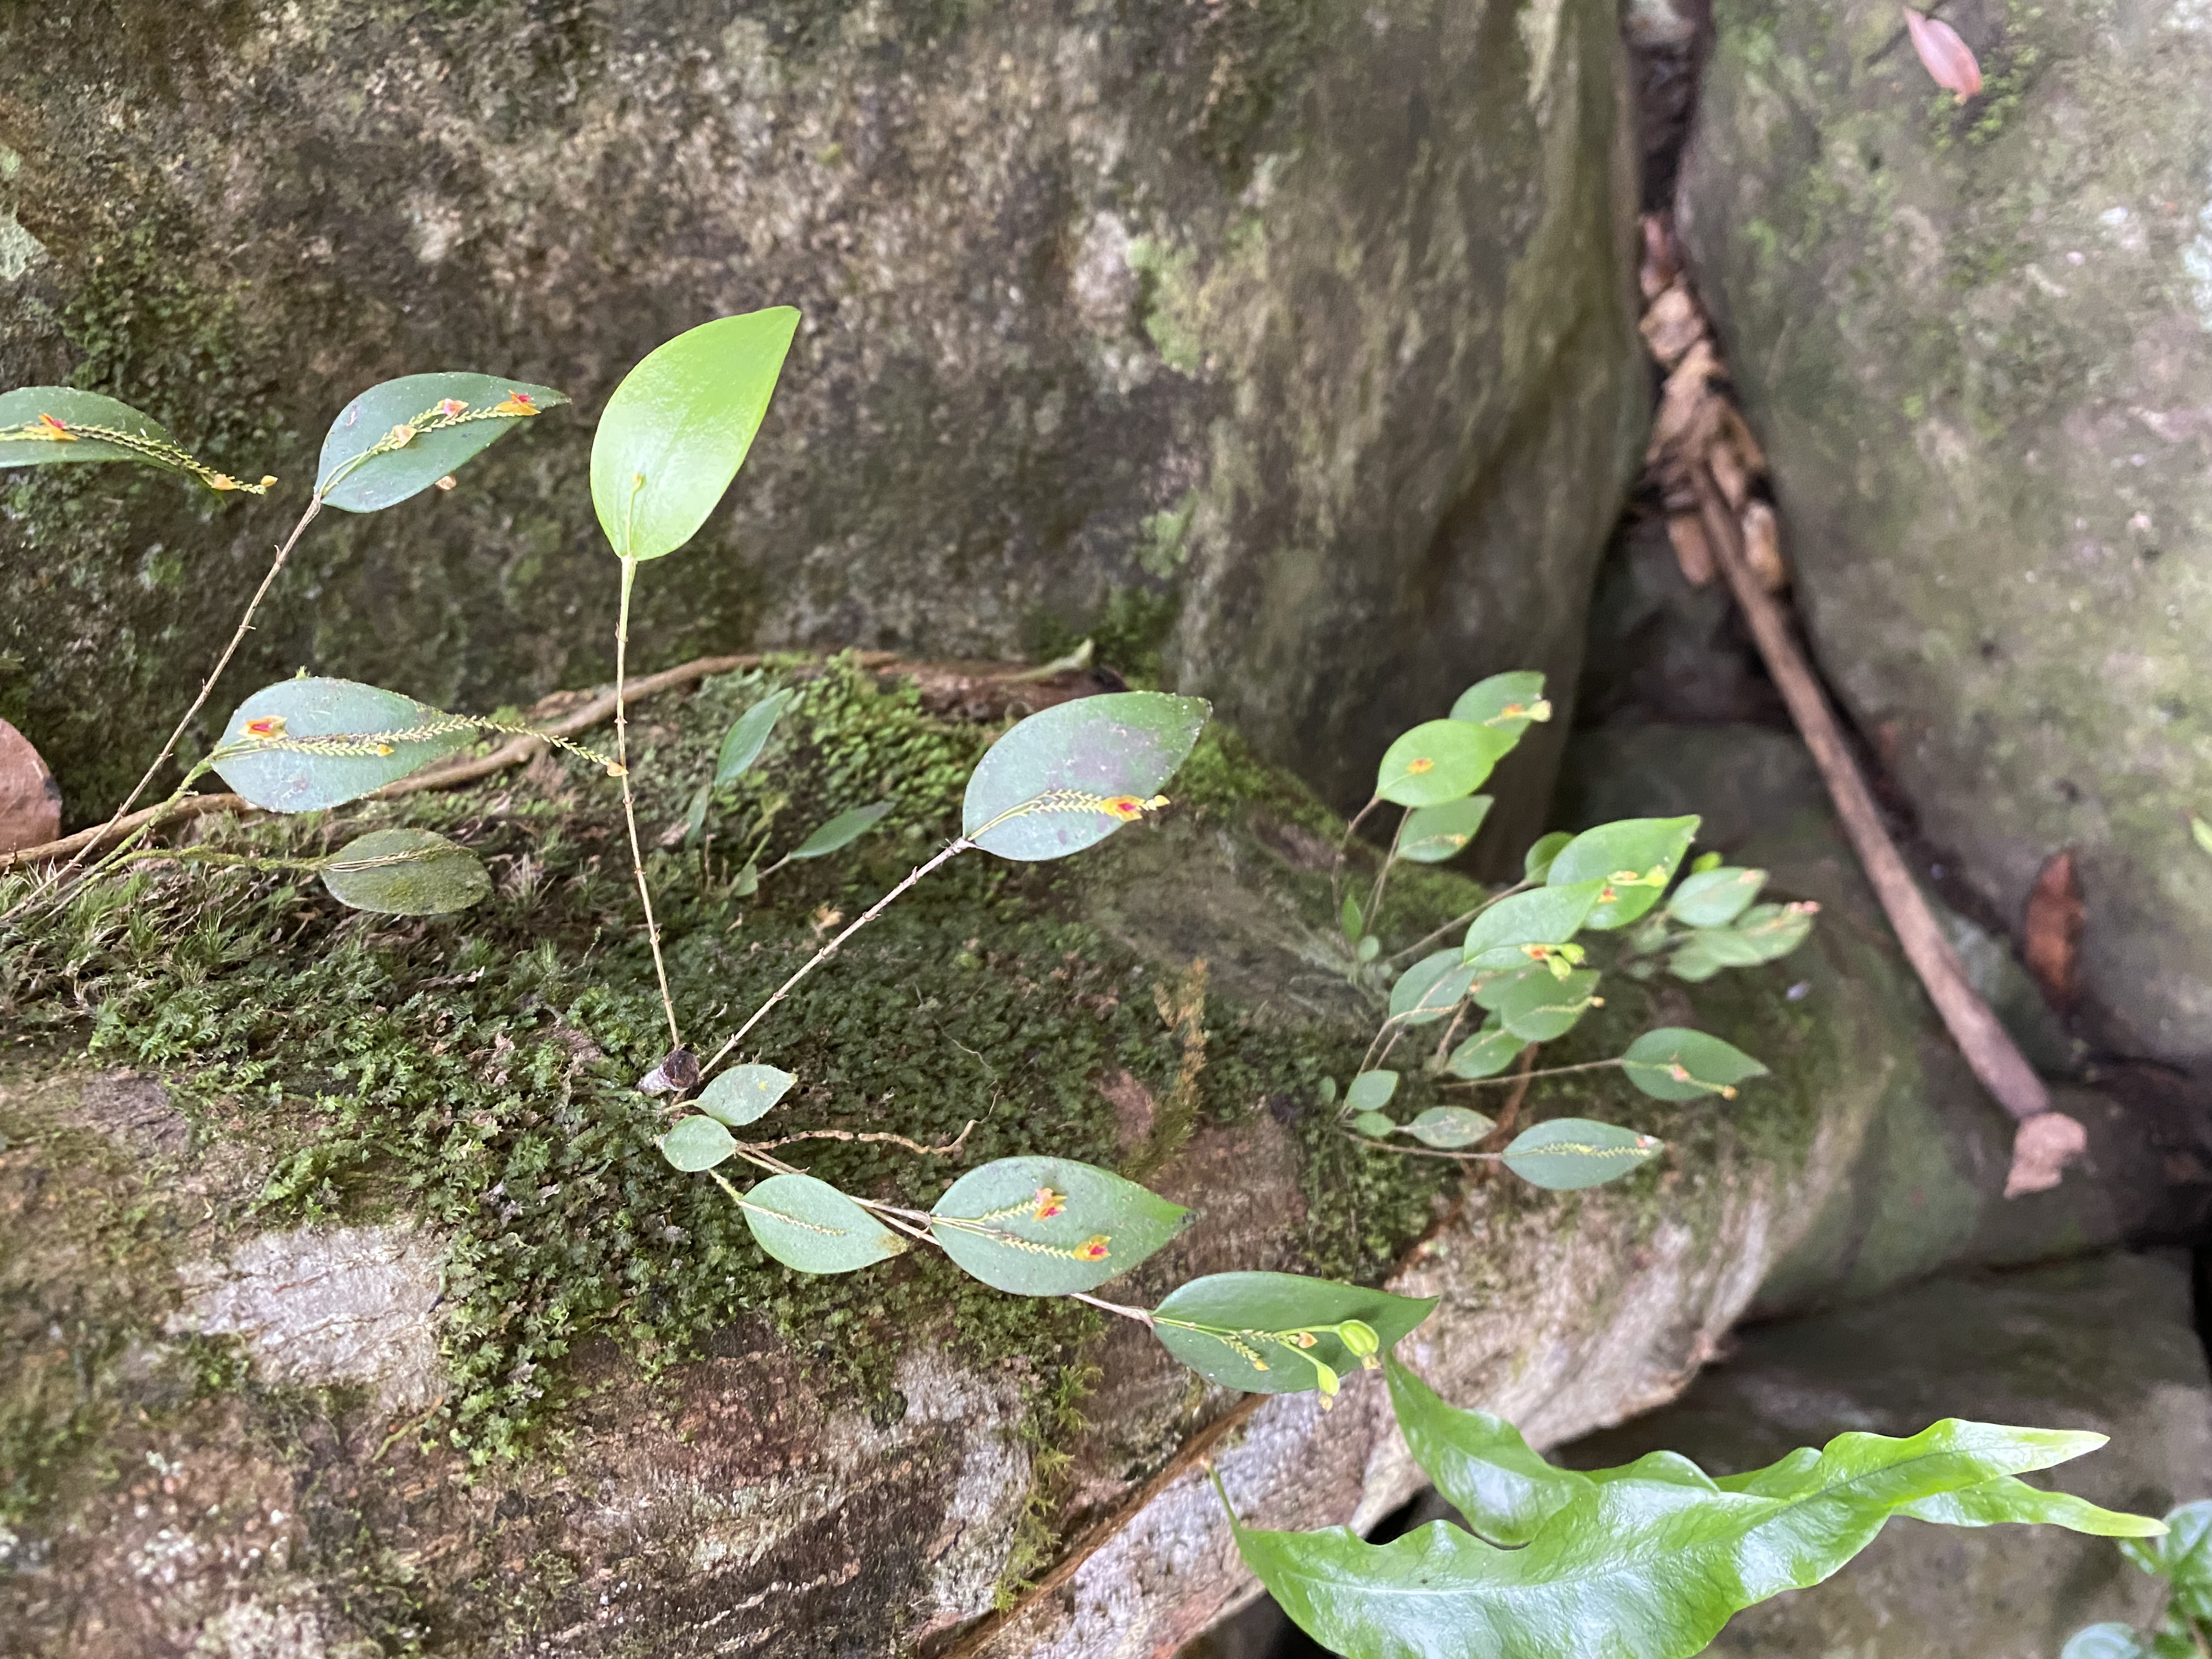
\includegraphics[keepaspectratio]{images/Lepanthes_rupestris_Tremblay.jpeg}}

}

\caption{\emph{Lepanthes rupestris}. Foto: Tremblay}

\end{figure}%

El ciclo de vida de \emph{L. rubripetala} fue dividido en cuatro
categorías de estado: plántula (PL), juvenil (J), adulto no reproductivo
(NR) y adulto reproductivo (AR). Esta última categoría florece y produce
frutos a largo de todo el año (Schödelbauerová, Tremblay \& Kindlmann,
2010; Tremblay, Raventos \& Ackerman, 2015). En consecuencia, la
estructura poblacional cuenta con una columna de 4 elementos, que
indican el número de individuos encontrado en el estado de plántula (0),
juvenil (46), adulto no reproductivo (38) y adulto reproductivo (82) al
inicio del estudio, indicado como \(t_{0}\) (Schödelbauerová, Tremblay
\& Kindlmann, 2010). Por su parte, la matriz de transición de \emph{L.
rubripetala} está formada por 4 renglones y 4 columnas (Tremblay,
Raventos \& Ackerman, 2015), que corresponden a los estados del ciclo de
vida de la especie y los 16 elementos de la probabilidad de permanencia,
transición a una categoría superior, retroceso a una categoría inferior
y fecundidad promedio por categoría (ver el capítulo de
\hyperref[MatricesT]{Transiciones}).

En el siguiente recuadro incorporamos la información de \emph{L.
rubripetala} en \emph{R}. La función \emph{matrix} fue usada para
construir la matriz de transición y \emph{n0} se usa para nombrar al
vector de la estructura inicial observada.

\begin{Shaded}
\begin{Highlighting}[]
\CommentTok{\#Capturar los datos de la matriz para L. rubripetala (Tremblay et al. 2015)}
\NormalTok{Lr1 }\OtherTok{\textless{}{-}} \FunctionTok{matrix}\NormalTok{(}\FunctionTok{c}\NormalTok{(}\FloatTok{0.4324}\NormalTok{, }\DecValTok{0}\NormalTok{,      }\DecValTok{0}\NormalTok{,     }\FloatTok{0.146}\NormalTok{,}
               \FloatTok{0.3784}\NormalTok{, }\FloatTok{0.8459}\NormalTok{, }\DecValTok{0}\NormalTok{,     }\DecValTok{0}\NormalTok{,}
               \DecValTok{0}\NormalTok{,      }\FloatTok{0.0034}\NormalTok{, }\FloatTok{0.7954}\NormalTok{,}\FloatTok{0.2300}\NormalTok{,}
               \DecValTok{0}\NormalTok{,      }\FloatTok{0.0890}\NormalTok{, }\FloatTok{0.1841}\NormalTok{,}\FloatTok{0.7510}\NormalTok{),}
      \AttributeTok{byrow=}\ConstantTok{TRUE}\NormalTok{,}\AttributeTok{ncol=}\DecValTok{4}\NormalTok{)}

\CommentTok{\#Capturar las categorías de estado}
\NormalTok{estadios }\OtherTok{\textless{}{-}} \FunctionTok{c}\NormalTok{(}\StringTok{"PL"}\NormalTok{, }\StringTok{"J"}\NormalTok{, }\StringTok{"NR"}\NormalTok{, }\StringTok{"AR"}\NormalTok{)}
\FunctionTok{colnames}\NormalTok{(Lr1) }\OtherTok{\textless{}{-}} \FunctionTok{rownames}\NormalTok{(Lr1) }\OtherTok{\textless{}{-}}\NormalTok{ estadios}

\CommentTok{\#Obtener la matriz L. rubripetala}
\NormalTok{Lr1 }\OtherTok{\textless{}{-}} \FunctionTok{matrix}\NormalTok{(Lr1[}\DecValTok{1}\SpecialCharTok{:}\DecValTok{4}\NormalTok{, ], }\AttributeTok{nrow =} \DecValTok{4}\NormalTok{, }\AttributeTok{dimnames =} \FunctionTok{list}\NormalTok{(estadios, estadios))}
\NormalTok{Lr1}
\end{Highlighting}
\end{Shaded}

\begin{verbatim}
       PL      J     NR    AR
PL 0.4324 0.0000 0.0000 0.146
J  0.3784 0.8459 0.0000 0.000
NR 0.0000 0.0034 0.7954 0.230
AR 0.0000 0.0890 0.1841 0.751
\end{verbatim}

Estructura de la población inicial

\begin{verbatim}
[1]  0 46 38 82
\end{verbatim}

\begin{center}\rule{0.5\linewidth}{0.5pt}\end{center}

\begin{enumerate}
\def\labelenumi{\alph{enumi})}
\setcounter{enumi}{1}
\tightlist
\item
  \emph{Crecimiento asintótico}. El crecimiento de la población de tipo
  asintótico, \(λ\) (de ahora en adelante \(λ_{max}\)), se estima en
  \emph{R} con la función \texttt{lambda}. Este crecimiento se alcanza a
  largo plazo si se mantienen las condiciones constantes de la
  población, y se evidencia cuando se mantiene constante o estable la
  proporción de individuos en la estructura poblacional.
\end{enumerate}

En el siguiente recuadro se calcula \(λ_{max}\) para la población 1 de
\emph{L. rubripetala}. El resultado indica que la tasa de crecimiento
poblacional es de 1.007. Esto implica que si existieran 1000 individuos
en la población, a esta tasa la población aumentaría en siete individuos
del primer mes (\(t_{0}\)) al siguiente (\(t_{1}\)). Este ejemplo sólo
permite ilustrar el concepto, ya que las poblaciones de \emph{Lepanthes}
nunca serán tan grandes en la naturaleza (Tremblay, 1997b).

\begin{Shaded}
\begin{Highlighting}[]
\CommentTok{\#Análisis asintótico (i.e. largo plazo) del crecimiento poblacional de L. rubripetala}
\CommentTok{\#La orquídea florece y produce frutos todo el año, por lo que el seguimiento de la población fue mensual.}

\CommentTok{\#PARÁMETROS POBLACIONALES}
\DocumentationTok{\#\#lambda: Tasa de crecimiento poblacional}

\NormalTok{lambda }\OtherTok{\textless{}{-}} \FunctionTok{lambda}\NormalTok{(Lr1)}
\NormalTok{lambda}
\end{Highlighting}
\end{Shaded}

\begin{verbatim}
[1] 1.006578
\end{verbatim}

\begin{center}\rule{0.5\linewidth}{0.5pt}\end{center}

\section{Análisis de la dinámica a corto
plazo}\label{anuxe1lisis-de-la-dinuxe1mica-a-corto-plazo}

El cálculo y análisis de la dinámica transitoria es menos directo en
comparación con la dinámica a largo plazo o asintótica (Stott, 2012).
Esto es, para distinguir los efectos transitorios de los asintóticos, en
la dinámica a corto plazo se plantean los siguientes análisis: la
dinámica poblacional absoluta, la dinámica transitoria estandarizada y
el cálculo de los límites transitorios. Debido a que la dinámica
transitoria depende de las condiciones iniciales de la estructura
(Raventós et~al., 2015), en la solución de estos tres análisis se
requiere definir el vector inicial para la población de estudio (Stott,
2012).

\subsection{Selección de la estructura poblacional
inicial}\label{selecciuxf3n-de-la-estructura-poblacional-inicial}

\emph{Modelo sesgado por categoría}. Stott y colaboradores (Stott
et~al., 2010a; Stott, Townley \& Hodgson, 2011) comentan que la
proyección de la dinámica transitoria o a corto plazo es muy sensible a
la estructura poblacional, así que lo mejor es hacer una selección
adecuada de este vector. Una opción es proyectar la dinámica transitoria
a partir de la abundancia de individuos observada al inicio del estudio,
denotada como \(n_{0}\), y otra es hacerlo a través de una selección de
cambios en la proporción de individuos por categoría (Stott, 2012). Con
la primera opción se describiría el caso específico de \emph{L.
rubripetala}, mientras que la segunda ofrece la opción de comparar los
resultados con otras especies al representar distintos escenarios que
ocurren o pueden ocurrir de forma aleatoria en la población de estudio
(Stott, 2012).

Las fluctuaciones aleatorias en la estructura debidas a una perturbación
de origen biótico, abiótico o antropogénico son incorporadas por Stott y
colaboradores como estocasticidad demográfica (Stott et~al., 2010a;
Stott, Townley \& Hodgson, 2011). Este tipo de estocasticidad se refiere
a la sobrevivencia y reproducción en número entero y finito; es decir,
un individuo sobrevive o no, lo cual se representa con 1 o 0, al igual
que puede reproducirse (1) o no (0). La incorporación de esta
característica en los individuos genera una variación no cíclica ni
predecible en la respuesta de los individuos de una población y pueden
tener un impacto considerable en el tamaño de la población (Stott,
2012).

Por ejemplo, la estructura inicial en la población 1 de \emph{L.
rubripetala} fue la siguiente: (0,46,38,82). En este caso, al modificar
la proporción de individuos presente en una, dos o en todas las
categorías de la población se simuló el cambio en la dinámica en el
corto plazo; es decir, en un momento previo a que se alcance el
crecimiento estable o a largo plazo. En \emph{L. rubripetala} se
hicieron cinco simulaciones o escenarios al suponer las siguientes
proporciones de individuos por categoría (Tremblay, Raventos \&
Ackerman, 2015):

\begin{tcolorbox}[enhanced jigsaw, arc=.35mm, bottomrule=.15mm, bottomtitle=1mm, breakable, colback=white, colbacktitle=quarto-callout-note-color!10!white, colframe=quarto-callout-note-color-frame, coltitle=black, left=2mm, leftrule=.75mm, opacityback=0, opacitybacktitle=0.6, rightrule=.15mm, title=\textcolor{quarto-callout-note-color}{\faInfo}\hspace{0.5em}{Nota}, titlerule=0mm, toprule=.15mm, toptitle=1mm]

\textbf{El análisis transitorio es sensible a la estructura inicial.} A
diferencia de λ, los índices transitorios (reactividad, amplificación,
atenuación, inercia) \textbf{cambian} según la composición inicial de la
población. Por eso la práctica recomendada es proyectar varios
escenarios:

\begin{itemize}
\tightlist
\item
  \textbf{Límites teóricos} (toda la población en una sola etapa) ---
  establecen el rango de comportamiento posible.
\item
  \textbf{Estructura observada} (\(n_0\)) --- muestra qué pasa con la
  población real al inicio del estudio.
\item
  \textbf{Estructura estable} (\(w\)) --- sirve como referencia de
  comparación.
\end{itemize}

Una población observada lejos de la estructura estable puede comportarse
de forma muy distinta a lo que predice λ.

\end{tcolorbox}

\subsubsection{Límite inferior}\label{luxedmite-inferior}

(1,0,0,0): todos los individuos de la población se encuentran en la
categoría de plántulas (\emph{lower bound}). Esto representa, por
ejemplo, una población que se está estableciendo, ya que todos los
individuos son plántulas y no hay individuos en las otras categorías.

\subsubsection{Inicio I}\label{inicio-i}

(0.15, 0.35, 0.30, 0.20): mayor proporción de individuos en las
categorías juvenil y adulto no reproductivo.

\subsubsection{Estructura estable de la
población}\label{estructura-estable-de-la-poblaciuxf3n}

Los individuos de la población tienen una abundancia de acuerdo con
\emph{w-max}.

\subsubsection{Inicio II}\label{inicio-ii}

(0.4, 0.2, 0.2, 0.2): mayor proporción de plántulas y una proporción
similar en las categorías juvenil, adulto no reproductivo y adulto
reproductivo.

\subsubsection{Límite superior}\label{luxedmite-superior}

(0,0,0,1): los individuos de la población se encuentran en la categoría
de adulto reproductivo. Esto representa, por ejemplo, una población que
se encuentra en su máximo potencial reproductivo, ya que todos los
individuos son adultos reproductivos. Esto pudiese representar una
población que tenga dificultad de producir nuevos individuos, es decir,
una población que se encuentra en un estado de declive.

\section{Dinámica poblacional
absoluta}\label{dinuxe1mica-poblacional-absoluta}

Como consecuencia de las perturbaciones o escenarios existen cambios en
el crecimiento poblacional, cuyas medidas absolutas de densidad
describen qué tan grande o pequeña puede llegar a ser una población en
el corto plazo (Stott, Townley \& Hodgson, 2011). Un aspecto importante
a considerar es que, estas medidas absolutas describen la influencia
combinada de las tasas de crecimiento transitorio y la dinámica
asintótica, cuyo comportamiento se conoce como dinámica poblacional
absoluta y se visualiza para \emph{L. rubripetala} a través de la figura
2A de Tremblay y colaboradores (Tremblay, Raventos \& Ackerman, 2015).

En los siguientes recuadros se proyecta la dinámica poblacional absoluta
de \emph{L. rubripetala} ante cambios en la estructura inicial
(\emph{i}-\emph{v}). Se estiman y grafican uno a uno los resultados de
los escenarios: 1, 3 y 5, por lo que se sugiere desarrollar los incisos
restantes, a fin de poner a prueba los conocimientos adquiridos.

\subsection{Proyección por
escenarios}\label{proyecciuxf3n-por-escenarios}

\subsubsection{Escenario 1 (límite
inferior):}\label{escenario-1-luxedmite-inferior}

Límite inferior (1,0,0,0): todos los individuos de la población se
encuentran en la categoría de plántulas (\emph{lower bound}). Esto
representa, por ejemplo, una población que se está estableciendo, ya que
todos los individuos son plántulas y no hay individuos en las otras
categorías.

En este caso, se observa que la población decrece rápidamente y se
estabiliza en un valor cercano a 0.6, lo que indica que el tamaño
relativo poblacional es menor que el tamaño poblacional del crecimiento
asintótico (1.007), aún después de proyectar su crecimiento a un
intervalo de 50 meses. A partir de lo anterior, se sugiere que la
población no se recupera y que la estructura de la población no es
favorable para el crecimiento poblacional de \emph{L. rubripetala}.

\begin{Shaded}
\begin{Highlighting}[]
\CommentTok{\# DINÁMICA POBLACIONAL ABSOLUTA.    }

\CommentTok{\#Definir los margenes}
\FunctionTok{par}\NormalTok{(}\AttributeTok{mfrow =} \FunctionTok{c}\NormalTok{(}\DecValTok{1}\NormalTok{, }\DecValTok{1}\NormalTok{))}
\FunctionTok{par}\NormalTok{(}\AttributeTok{mar =} \FunctionTok{c}\NormalTok{(}\DecValTok{3}\NormalTok{, }\DecValTok{3}\NormalTok{, }\DecValTok{3}\NormalTok{, }\DecValTok{3}\NormalTok{))}

\CommentTok{\#Vector original}
\NormalTok{nLr0 }\OtherTok{\textless{}{-}} \FunctionTok{c}\NormalTok{(}\DecValTok{0}\NormalTok{, }\DecValTok{46}\NormalTok{, }\DecValTok{38}\NormalTok{, }\DecValTok{82}\NormalTok{)}
\CommentTok{\#Escenario 1. Límite inferior \# Límite inferior (1,0,0,0)}
\NormalTok{nLr1 }\OtherTok{\textless{}{-}} \FunctionTok{c}\NormalTok{(}\DecValTok{166}\NormalTok{, }\DecValTok{0}\NormalTok{, }\DecValTok{0}\NormalTok{, }\DecValTok{0}\NormalTok{)}
\CommentTok{\#Proporción de individuos por categoría}
\NormalTok{nLr1 }\OtherTok{\textless{}{-}}\NormalTok{ nLr1 }\SpecialCharTok{/} \FunctionTok{sum}\NormalTok{(nLr1)}
\CommentTok{\# nLr1}
\CommentTok{\#Gráfica de barras del escenario 1}
\CommentTok{\#barplot(nLr1, names.arg = 1:4)}
\CommentTok{\#title(main = "Escenario 1", xlab = "Categoría", ylab = "Proporción")}
\CommentTok{\#Proyección de la dinámica escenario 1}
\NormalTok{pr1 }\OtherTok{\textless{}{-}} \FunctionTok{project}\NormalTok{(Lr1, }\AttributeTok{vector =}\NormalTok{ nLr1, }\AttributeTok{time =} \DecValTok{50}\NormalTok{)}

\NormalTok{pr1df }\OtherTok{\textless{}{-}} \FunctionTok{as.data.frame}\NormalTok{(pr1)}

\NormalTok{pr1df}\SpecialCharTok{$}\NormalTok{time }\OtherTok{\textless{}{-}} \FunctionTok{seq}\NormalTok{(}\DecValTok{1}\NormalTok{, }\FunctionTok{nrow}\NormalTok{(pr1df), }\DecValTok{1}\NormalTok{)}

\FunctionTok{ggplot}\NormalTok{(pr1df, }\FunctionTok{aes}\NormalTok{(time, pr1)) }\SpecialCharTok{+}
  \FunctionTok{geom\_line}\NormalTok{(}\FunctionTok{aes}\NormalTok{(}\AttributeTok{color =} \StringTok{"blue"}\NormalTok{), }\AttributeTok{size =} \DecValTok{2}\NormalTok{) }\SpecialCharTok{+}
  \FunctionTok{geom\_hline}\NormalTok{(}\AttributeTok{yintercept =} \DecValTok{1}\NormalTok{, }\AttributeTok{linetype =} \StringTok{"dashed"}\NormalTok{, }\AttributeTok{color =} \StringTok{"red"}\NormalTok{) }\SpecialCharTok{+}
  \FunctionTok{xlab}\NormalTok{(}\StringTok{"Time intervals"}\NormalTok{) }\SpecialCharTok{+}
  \FunctionTok{ylab}\NormalTok{(}\StringTok{"Relative population size/density"}\NormalTok{) }\SpecialCharTok{+}
  \FunctionTok{theme\_minimal}\NormalTok{() }\SpecialCharTok{+}
  \FunctionTok{rlt\_style\_colour}\NormalTok{()}\SpecialCharTok{+}
  \FunctionTok{theme}\NormalTok{(}\AttributeTok{legend.position =} \StringTok{"none"}\NormalTok{)}
\end{Highlighting}
\end{Shaded}

\pandocbounded{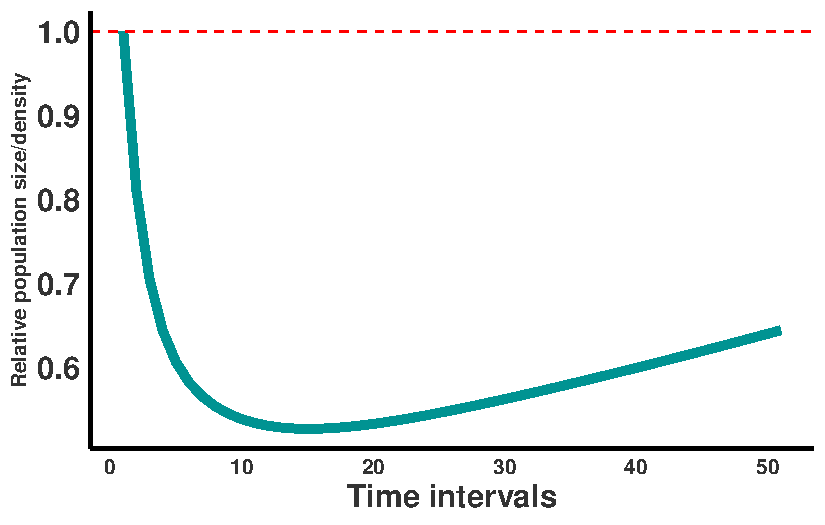
\includegraphics[keepaspectratio]{112-Dinamica_de_Transiciones_files/figure-pdf/trans4-1.pdf}}

\begin{Shaded}
\begin{Highlighting}[]
\CommentTok{\#plot(pr1, log = "y", ylim = c(0.1, 1.6), ann = FALSE)}
\CommentTok{\#title(main = "Proyección de la dinámica (Escenario 1)", xlab = "Time intervals", ylab = "Population size/density")}
\end{Highlighting}
\end{Shaded}

\begin{center}\rule{0.5\linewidth}{0.5pt}\end{center}

\subsubsection{Segundo escenario:}\label{segundo-escenario}

En este escenario, se supone que la población tiene una mayor proporción
de individuos en las categorías juvenil y adulto no reproductivo (0.15,
0.35, 0.30, 0.20). En este caso, la población decrece rápidamente en los
primeros periodos, pero después de unos 5 periodos de tiempo la
población comienza a crecer y alcanza un tamaño poblacional relativo
similar al comienzo después de ±16 periodos de tiempo. Esto indica que
la población se recupera rápidamente y alcanza un tamaño poblacional
estable en un periodo relativamente corto.

\begin{center}\rule{0.5\linewidth}{0.5pt}\end{center}

\subsubsection{Tercer escenario (estructura
estable):}\label{tercer-escenario-estructura-estable}

Como la población tiene una estructura estable, la población no tiene un
crecimiento diferente a 1, por lo que alcanza un tamaño poblacional
estable en un periodo relativamente corto o inmediato. Debido a que la
población tiene una estructura estable, el tamaño relativo de la
población es constante.

\begin{Shaded}
\begin{Highlighting}[]
\CommentTok{\#Escenario 3. Estructura estable}
\CommentTok{\# Estructura estable de estados}
\NormalTok{Wmax }\OtherTok{\textless{}{-}} \FunctionTok{stable.stage}\NormalTok{(Lr1)}
\NormalTok{nLr3 }\OtherTok{\textless{}{-}}\NormalTok{ Wmax}
\CommentTok{\#Gráfica de barras del escenario 3}
\CommentTok{\#barplot(nLr3, names.arg = 1:4)}
\CommentTok{\#title( main = "Escenario 3", xlab = "Categoría", ylab = "Proporción")}
\CommentTok{\#Proyección de la dinámica escenario 3}
\NormalTok{Lr1st }\OtherTok{\textless{}{-}}\NormalTok{ (Lr1 }\SpecialCharTok{/}\NormalTok{ lambda)}
\CommentTok{\#Lr1st}
\CommentTok{\#eigen(Lr1st)}
\NormalTok{pr3 }\OtherTok{\textless{}{-}} \FunctionTok{project}\NormalTok{(Lr1st, }\AttributeTok{vector =}\NormalTok{ Wmax, }\AttributeTok{time =} \DecValTok{50}\NormalTok{)}
\NormalTok{pr3df }\OtherTok{\textless{}{-}} \FunctionTok{as.data.frame}\NormalTok{(pr3)}
\NormalTok{pr3df}\SpecialCharTok{$}\NormalTok{time }\OtherTok{\textless{}{-}} \FunctionTok{seq}\NormalTok{(}\DecValTok{1}\NormalTok{, }\FunctionTok{nrow}\NormalTok{(pr3df), }\DecValTok{1}\NormalTok{)}
\FunctionTok{ggplot}\NormalTok{(pr3df, }\FunctionTok{aes}\NormalTok{(time, pr3)) }\SpecialCharTok{+}
  \FunctionTok{geom\_line}\NormalTok{(}\FunctionTok{aes}\NormalTok{(}\AttributeTok{color =} \StringTok{"blue"}\NormalTok{), }\AttributeTok{size =} \DecValTok{2}\NormalTok{) }\SpecialCharTok{+}
  \FunctionTok{geom\_hline}\NormalTok{(}\AttributeTok{yintercept =} \DecValTok{1}\NormalTok{, }\AttributeTok{linetype =} \StringTok{"dashed"}\NormalTok{, }\AttributeTok{color =} \StringTok{"red"}\NormalTok{) }\SpecialCharTok{+}
  \FunctionTok{xlab}\NormalTok{(}\StringTok{"Time intervals"}\NormalTok{) }\SpecialCharTok{+}
  \FunctionTok{ylab}\NormalTok{(}\StringTok{"Relative population size/density"}\NormalTok{) }\SpecialCharTok{+}
  \FunctionTok{theme\_minimal}\NormalTok{() }\SpecialCharTok{+}
  \FunctionTok{rlt\_style\_colour}\NormalTok{()}
\end{Highlighting}
\end{Shaded}

\pandocbounded{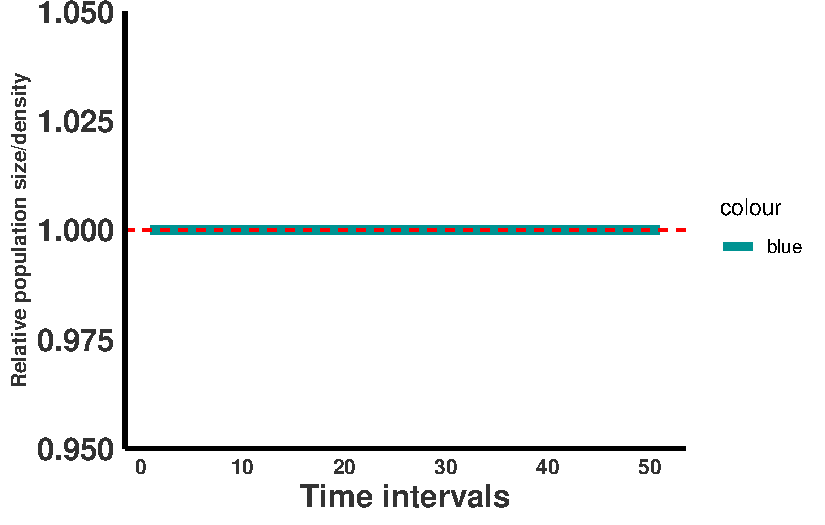
\includegraphics[keepaspectratio]{112-Dinamica_de_Transiciones_files/figure-pdf/trans6-1.pdf}}

\begin{Shaded}
\begin{Highlighting}[]
\DocumentationTok{\#\# Código para el plot usando el método tradicional}

\CommentTok{\#plot(pr3, log = "y", ylim = c(0.1, 1.6), ann = FALSE)}
\CommentTok{\#title(main = "Proyección de la dinámica (Escenario 3)", xlab = "Time intervals", ylab = "Population size/density")}
\end{Highlighting}
\end{Shaded}

\begin{center}\rule{0.5\linewidth}{0.5pt}\end{center}

\subsubsection{Cuarto escenario:}\label{cuarto-escenario}

En este escenario, se supone que la población tiene una mayor proporción
de plántulas y una proporción similar en las categorías juvenil, adulto
no reproductivo y adulto reproductivo (0.4, 0.2, 0.2, 0.2). En este
caso, la población decrece rápidamente en los primeros periodos, pero
después de unos ±7 periodos de tiempo la población comienza a crecer y
alcanza un tamaño poblacional relativo similar al comienzo después de
±36 periodos de tiempo. Esto indica que la población se recupera
rápidamente y alcanza un tamaño poblacional estable en un periodo
relativamente corto, si la población comienza con esta estructura
demográfica.

\begin{Shaded}
\begin{Highlighting}[]
\CommentTok{\# DINÁMICA POBLACIONAL ABSOLUTA.}

\NormalTok{nLr4 }\OtherTok{\textless{}{-}} \FunctionTok{c}\NormalTok{(}\DecValTok{66}\NormalTok{, }\DecValTok{33}\NormalTok{, }\DecValTok{33}\NormalTok{, }\DecValTok{33}\NormalTok{)}
\NormalTok{nLr4 }\OtherTok{\textless{}{-}}\NormalTok{ nLr4 }\SpecialCharTok{/} \FunctionTok{sum}\NormalTok{(nLr4)}

\NormalTok{pr4 }\OtherTok{\textless{}{-}} \FunctionTok{project}\NormalTok{(Lr1, }\AttributeTok{vector =}\NormalTok{ nLr4, }\AttributeTok{time =} \DecValTok{50}\NormalTok{)}
\NormalTok{pr4df }\OtherTok{\textless{}{-}} \FunctionTok{as.data.frame}\NormalTok{(pr4)}
\NormalTok{pr4df}\SpecialCharTok{$}\NormalTok{time }\OtherTok{\textless{}{-}} \FunctionTok{seq}\NormalTok{(}\DecValTok{1}\NormalTok{, }\FunctionTok{nrow}\NormalTok{(pr4df), }\DecValTok{1}\NormalTok{)}
\end{Highlighting}
\end{Shaded}

\begin{center}\rule{0.5\linewidth}{0.5pt}\end{center}

\subsubsection{Quinto escenario:}\label{quinto-escenario}

En este escenario, se supone que la población tiene una mayor proporción
de individuos en la categoría de adulto reproductivo (0,0,0,1). En el
escenario 5, la población crece rápidamente en los primeros periodos,
sufriendo una reducción después de ±5 meses; no obstante, se reconoce
que la población aumenta rápidamente.

\begin{Shaded}
\begin{Highlighting}[]
\CommentTok{\#Escenario 5. Límite superior}
\NormalTok{nLr5 }\OtherTok{\textless{}{-}} \FunctionTok{c}\NormalTok{(}\DecValTok{0}\NormalTok{, }\DecValTok{0}\NormalTok{, }\DecValTok{0}\NormalTok{, }\DecValTok{166}\NormalTok{)}
\CommentTok{\#Proporción de individuos por categoría}
\NormalTok{nLr5 }\OtherTok{\textless{}{-}}\NormalTok{ nLr5 }\SpecialCharTok{/} \FunctionTok{sum}\NormalTok{(nLr5)}
\CommentTok{\#nLr5}
\CommentTok{\#Gráfica de barras del escenario 5}
\CommentTok{\#barplot(nLr5, names.arg = 1:4)}
\CommentTok{\#title( main = "Escenario 5", xlab = "Categoría", ylab = "Proporción")}
\CommentTok{\#Proyección de la dinámica escenario 5}
\NormalTok{pr5 }\OtherTok{\textless{}{-}} \FunctionTok{project}\NormalTok{(Lr1, }\AttributeTok{vector =}\NormalTok{ nLr5, }\AttributeTok{time =} \DecValTok{50}\NormalTok{)}
\NormalTok{pr5df }\OtherTok{\textless{}{-}} \FunctionTok{as.data.frame}\NormalTok{(pr5)}
\NormalTok{pr5df}\SpecialCharTok{$}\NormalTok{time }\OtherTok{\textless{}{-}} \FunctionTok{seq}\NormalTok{(}\DecValTok{1}\NormalTok{, }\FunctionTok{nrow}\NormalTok{(pr5df), }\DecValTok{1}\NormalTok{)}
\FunctionTok{ggplot}\NormalTok{(pr5df, }\FunctionTok{aes}\NormalTok{(time, pr5)) }\SpecialCharTok{+}
  \FunctionTok{geom\_line}\NormalTok{(}\FunctionTok{aes}\NormalTok{(}\AttributeTok{color =} \StringTok{"blue"}\NormalTok{), }\AttributeTok{size =} \DecValTok{2}\NormalTok{) }\SpecialCharTok{+}
  \FunctionTok{geom\_hline}\NormalTok{(}\AttributeTok{yintercept =} \DecValTok{1}\NormalTok{, }\AttributeTok{linetype =} \StringTok{"dashed"}\NormalTok{, }\AttributeTok{color =} \StringTok{"red"}\NormalTok{) }\SpecialCharTok{+}
  \FunctionTok{xlab}\NormalTok{(}\StringTok{"Time intervals"}\NormalTok{) }\SpecialCharTok{+}
  \FunctionTok{ylab}\NormalTok{(}\StringTok{"Relative population size/density"}\NormalTok{) }\SpecialCharTok{+}
  \FunctionTok{theme\_minimal}\NormalTok{() }\SpecialCharTok{+}
  \FunctionTok{rlt\_style\_colour}\NormalTok{()}
\end{Highlighting}
\end{Shaded}

\pandocbounded{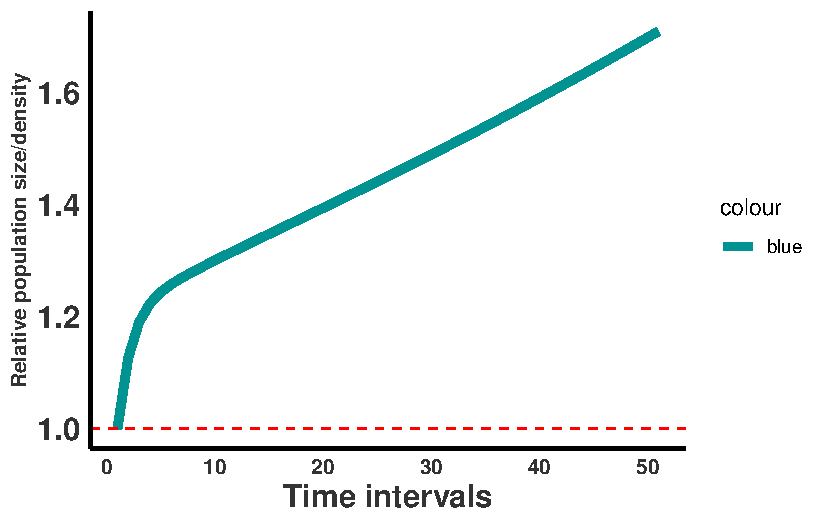
\includegraphics[keepaspectratio]{112-Dinamica_de_Transiciones_files/figure-pdf/trans8-1.pdf}}

\begin{Shaded}
\begin{Highlighting}[]
\CommentTok{\#plot(pr5, log = "y", ylim = c(0.1, 1.6), ann = FALSE)}
\CommentTok{\#title(main = "Proyección de la dinámica (Escenario 5)", xlab = "Time intervals", ylab = "Population size/density")}
\end{Highlighting}
\end{Shaded}

\begin{center}\rule{0.5\linewidth}{0.5pt}\end{center}

\subsection{Gráfica de la dinámica absoluta escenario 1, 3 y
5}\label{gruxe1fica-de-la-dinuxe1mica-absoluta-escenario-1-3-y-5}

En el siguiente recuadro se integran en una sola gráfica los resultados
de la dinámica absoluta de \emph{L. rubripetala} para los escenarios 1,
3 y 5.

\begin{Shaded}
\begin{Highlighting}[]
\FunctionTok{ggplot}\NormalTok{(Population\_density, }\FunctionTok{aes}\NormalTok{(time, Pop, }\AttributeTok{color =}\NormalTok{ Escenario)) }\SpecialCharTok{+}
  \FunctionTok{geom\_line}\NormalTok{(}\AttributeTok{size =} \DecValTok{1}\NormalTok{) }\SpecialCharTok{+}
  \FunctionTok{geom\_hline}\NormalTok{(}\AttributeTok{yintercept =} \DecValTok{1}\NormalTok{, }\AttributeTok{linetype =} \StringTok{"dashed"}\NormalTok{, }\AttributeTok{color =} \StringTok{"red"}\NormalTok{) }\SpecialCharTok{+}
  \FunctionTok{labs}\NormalTok{(}
    \AttributeTok{title =} \StringTok{"Population dynamics projections"}\NormalTok{,}
    \AttributeTok{x =} \StringTok{"Time intervals"}\NormalTok{,}
    \AttributeTok{y =} \StringTok{"Relative population size/density"}
\NormalTok{  ) }\SpecialCharTok{+}
  \FunctionTok{theme\_minimal}\NormalTok{() }\SpecialCharTok{+}
  \FunctionTok{rlt\_style\_colour}\NormalTok{()}
\end{Highlighting}
\end{Shaded}

\pandocbounded{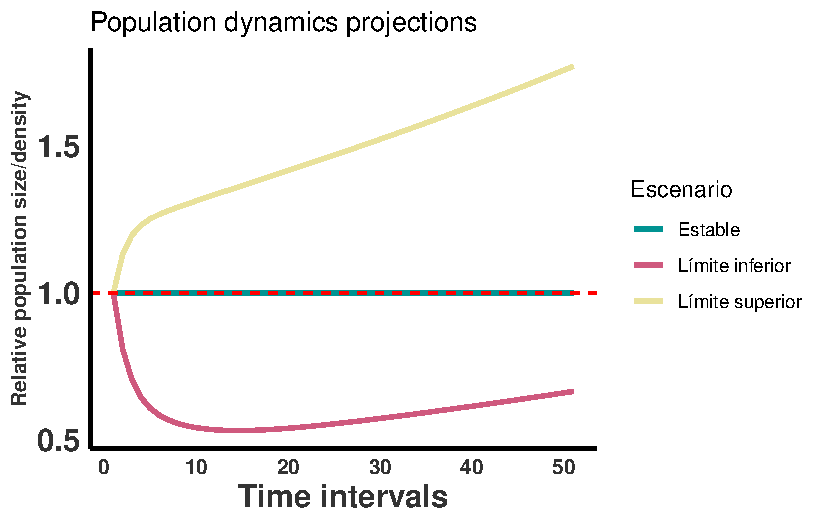
\includegraphics[keepaspectratio]{112-Dinamica_de_Transiciones_files/figure-pdf/trans10-1.pdf}}

\begin{center}\rule{0.5\linewidth}{0.5pt}\end{center}

\begin{center}\rule{0.5\linewidth}{0.5pt}\end{center}

\section{Dinámica poblacional transitoria
estandarizada}\label{dinuxe1mica-poblacional-transitoria-estandarizada}

\begin{tcolorbox}[enhanced jigsaw, arc=.35mm, bottomrule=.15mm, bottomtitle=1mm, breakable, colback=white, colbacktitle=quarto-callout-tip-color!10!white, colframe=quarto-callout-tip-color-frame, coltitle=black, left=2mm, leftrule=.75mm, opacityback=0, opacitybacktitle=0.6, rightrule=.15mm, title=\textcolor{quarto-callout-tip-color}{\faLightbulb}\hspace{0.5em}{Recomendación}, titlerule=0mm, toprule=.15mm, toptitle=1mm]

\textbf{Estandarizar permite comparar escenarios sin que λ los domine.}
Cuando se proyecta la dinámica absoluta de varios escenarios iniciales,
la trayectoria que más crece es siempre la que más se acerca a la
estructura estable --- porque después de unos pocos pasos todas crecen
al ritmo asintótico λ. Para aislar \textbf{el efecto de la estructura
inicial}, se divide la matriz por λ y se escala el vector inicial a
sumar 1. Las trayectorias resultantes muestran sólo la respuesta
transitoria, lo que las hace \textbf{directamente comparables} entre
escenarios y entre poblaciones de distintas especies.

\end{tcolorbox}

La dinámica poblacional transitoria estandarizada proyecta de forma
cuantitativa los cambios en la población a corto plazo para los
escenarios planteados. Con este fin, primero se elimina el efecto a
largo plazo de la tasa de crecimiento poblacional y de la estructura
inicial de la población, lo cual permite mantener otras propiedades
asintóticas, por ejemplo, la estructura estable de estados/edades y las
elasticidades (Koons, Iles \& Stott, 2021). En este proceso se dividen
todos los elementos de la matriz sobre el valor de la lambda asintótica
(\(λ_{max}\)) obtenida por la iteración de la matriz y se escala a 1 el
vector de la estructura poblacional (Koons, Iles \& Stott, 2021). Como
resultado de este proceso, y para cualquier matriz y vector
estandarizados, tendremos una \(λ_{max}\) igual a la unidad y la suma de
1 en el segundo caso, lo cual facilita y hace equitativa la comparación
entre los modelos de los distintos escenarios (Stott, Townley \&
Hodgson, 2011; Stott, Hodgson \& Townley, 2012b; Stott, Hodgson \&
Townley, 2012a; Koons, Iles \& Stott, 2021).

En el artículo de Tremblay y colaboradores (Tremblay, Raventos \&
Ackerman, 2015), la dinámica transitoria para \emph{L. rubripetala}
corresponde a la figura 2B. Esta figura se construye con base en la
matriz y vectores estandarizados de los cinco escenarios definidos y se
proyecta el crecimiento de la población a 50 meses (4.1 años). Las
gráficas de la dinámica transitoria para estos escenarios se generan
usando las siguientes funciones de \emph{R}:
\texttt{standard.A\ =\ TRUE} en la estandarización de la matriz y
\texttt{standard.vec\ =\ TRUE} para el vector, \texttt{project()} para
estimar la tendencia del crecimiento poblacional (Stott, Townley \&
Hodgson, 2011; Stott, Hodgson \& Townley, 2012b; Stott, Hodgson \&
Townley, 2012a) y \texttt{ggplot2} para agrupar en una sola gráfica la
tendencia del crecimiento poblacional de los escenarios.

En el siguiente recuadro se estima el crecimiento poblacional de
\emph{L. rubripetala} sin efecto de la dinámica asintótica para tres
escenarios: 1, 3 y 5. En el cálculo de la dinámica a corto plazo se
proyecta usando la matriz de transición de la población 1 de \emph{L.
rubripetala} y el correspondiente vector inicial de la población.

\begin{Shaded}
\begin{Highlighting}[]
\DocumentationTok{\#\# PROYECCIÓN DE LA DINÁMICA A CORTO PLAZO.}

\CommentTok{\#Vector de estructura inicial: abundancia por categoría de acuerdo con  el estado}
\NormalTok{n0 }\OtherTok{\textless{}{-}} \FunctionTok{c}\NormalTok{(}\DecValTok{166}\NormalTok{, }\DecValTok{0}\NormalTok{, }\DecValTok{0}\NormalTok{, }\DecValTok{0}\NormalTok{)}

\CommentTok{\#Escenario 1: Límite inferior}
\NormalTok{pr2}\FloatTok{.1} \OtherTok{\textless{}{-}} \FunctionTok{project}\NormalTok{(}
\NormalTok{  Lr1,}
  \AttributeTok{vector =}\NormalTok{ nLr1,}
  \AttributeTok{time =} \DecValTok{50}\NormalTok{,}
  \AttributeTok{standard.A =}\NormalTok{ T,}
  \AttributeTok{standard.vec =}\NormalTok{ T}
\NormalTok{)}

\CommentTok{\#Escenario 3. Estructura estable}
\NormalTok{pr2}\FloatTok{.3} \OtherTok{\textless{}{-}} \FunctionTok{project}\NormalTok{(}
\NormalTok{  Lr1,}
  \AttributeTok{vector =}\NormalTok{ nLr3,}
  \AttributeTok{time =} \DecValTok{50}\NormalTok{,}
  \AttributeTok{standard.A =}\NormalTok{ T,}
  \AttributeTok{standard.vec =}\NormalTok{ T}
\NormalTok{)}

\CommentTok{\#Escenario 5. Límite superior}
\NormalTok{pr2}\FloatTok{.5} \OtherTok{\textless{}{-}} \FunctionTok{project}\NormalTok{(}
\NormalTok{  Lr1,}
  \AttributeTok{vector =}\NormalTok{ nLr5,}
  \AttributeTok{time =} \DecValTok{50}\NormalTok{,}
  \AttributeTok{standard.A =}\NormalTok{ T,}
  \AttributeTok{standard.vec =}\NormalTok{ T}
\NormalTok{)}
\end{Highlighting}
\end{Shaded}

\begin{center}\rule{0.5\linewidth}{0.5pt}\end{center}

\section{Gráfica de la dinámica poblacional transitoria estandarizada
por
escenario}\label{gruxe1fica-de-la-dinuxe1mica-poblacional-transitoria-estandarizada-por-escenario}

La proyección de la dinámica transitoria para los tres escenarios
definidos (1, 3, y 5) tiene un comportamiento contrastante, lo cual es
evidente en la gráfica del siguiente recuadro. El crecimiento es
constante (i.e.~lambda =1) cuando se considera la estructura estable de
estados. Cuando la estructura poblacional corresponde al Inicio I se
determina un decremento en la población en los primeros 5 meses, el cual
se mantiene en el tiempo a lo largo de la proyección. Si la población
está representada por adultos reproductivos, ésta crece en los primeros
cinco meses y este crecimiento se mantiene a lo largo de los 50 meses.

\begin{Shaded}
\begin{Highlighting}[]
\CommentTok{\# DINÁMICA POBLACIONAL TRANSITORIA ESTANDARIZADA {-}{-}{-}{-}{-}{-}{-}{-}{-}{-} \#}
\CommentTok{\# Gráfica de la Dinámica transitoria específica de la población  }

\FunctionTok{layout}\NormalTok{(}\FunctionTok{matrix}\NormalTok{(}\FunctionTok{c}\NormalTok{(}\DecValTok{1}\NormalTok{, }\DecValTok{2}\NormalTok{, }\DecValTok{3}\NormalTok{), }\AttributeTok{ncol =} \DecValTok{3}\NormalTok{))}

\CommentTok{\# Escenario 2}
\NormalTok{yr }\OtherTok{\textless{}{-}} \FunctionTok{safe\_log\_ylim}\NormalTok{(}\FunctionTok{as.numeric}\NormalTok{(pr2}\FloatTok{.2}\NormalTok{))}
\FunctionTok{plot}\NormalTok{(pr2}\FloatTok{.2}\NormalTok{, }\AttributeTok{log =} \StringTok{"y"}\NormalTok{, }\AttributeTok{main =} \StringTok{"Escenario 2"}\NormalTok{, }\AttributeTok{xlab =} \StringTok{""}\NormalTok{, }\AttributeTok{ylab =} \StringTok{"Densidad poblacional"}\NormalTok{,}
     \AttributeTok{ylim =}\NormalTok{ yr, }\AttributeTok{yaxt =} \StringTok{"n"}\NormalTok{)}
\FunctionTok{axis}\NormalTok{(}\DecValTok{2}\NormalTok{, }\AttributeTok{at =} \FunctionTok{safe\_log\_ticks}\NormalTok{(yr), }\AttributeTok{labels =} \FunctionTok{signif}\NormalTok{(}\FunctionTok{safe\_log\_ticks}\NormalTok{(yr), }\DecValTok{3}\NormalTok{))}

\CommentTok{\# Escenario 3 (constante ≈ 1 → needs padding)}
\NormalTok{yr }\OtherTok{\textless{}{-}} \FunctionTok{safe\_log\_ylim}\NormalTok{(}\FunctionTok{as.numeric}\NormalTok{(pr2}\FloatTok{.3}\NormalTok{))}
\FunctionTok{plot}\NormalTok{(pr2}\FloatTok{.3}\NormalTok{, }\AttributeTok{log =} \StringTok{"y"}\NormalTok{, }\AttributeTok{main =} \StringTok{"Escenario 3"}\NormalTok{, }\AttributeTok{xlab =} \StringTok{""}\NormalTok{, }\AttributeTok{ylab =} \StringTok{""}\NormalTok{,}
     \AttributeTok{ylim =}\NormalTok{ yr, }\AttributeTok{yaxt =} \StringTok{"n"}\NormalTok{)}
\FunctionTok{axis}\NormalTok{(}\DecValTok{2}\NormalTok{, }\AttributeTok{at =} \FunctionTok{safe\_log\_ticks}\NormalTok{(yr), }\AttributeTok{labels =} \FunctionTok{signif}\NormalTok{(}\FunctionTok{safe\_log\_ticks}\NormalTok{(yr), }\DecValTok{3}\NormalTok{))}

\CommentTok{\# Escenario 5}
\NormalTok{yr }\OtherTok{\textless{}{-}} \FunctionTok{safe\_log\_ylim}\NormalTok{(}\FunctionTok{as.numeric}\NormalTok{(pr2}\FloatTok{.5}\NormalTok{))}
\FunctionTok{plot}\NormalTok{(pr2}\FloatTok{.5}\NormalTok{, }\AttributeTok{log =} \StringTok{"y"}\NormalTok{, }\AttributeTok{main =} \StringTok{"Escenario 5"}\NormalTok{, }\AttributeTok{xlab =} \StringTok{""}\NormalTok{, }\AttributeTok{ylab =} \StringTok{""}\NormalTok{,}
     \AttributeTok{ylim =}\NormalTok{ yr, }\AttributeTok{yaxt =} \StringTok{"n"}\NormalTok{)}
\FunctionTok{axis}\NormalTok{(}\DecValTok{2}\NormalTok{, }\AttributeTok{at =} \FunctionTok{safe\_log\_ticks}\NormalTok{(yr), }\AttributeTok{labels =} \FunctionTok{signif}\NormalTok{(}\FunctionTok{safe\_log\_ticks}\NormalTok{(yr), }\DecValTok{3}\NormalTok{))}
\end{Highlighting}
\end{Shaded}

\pandocbounded{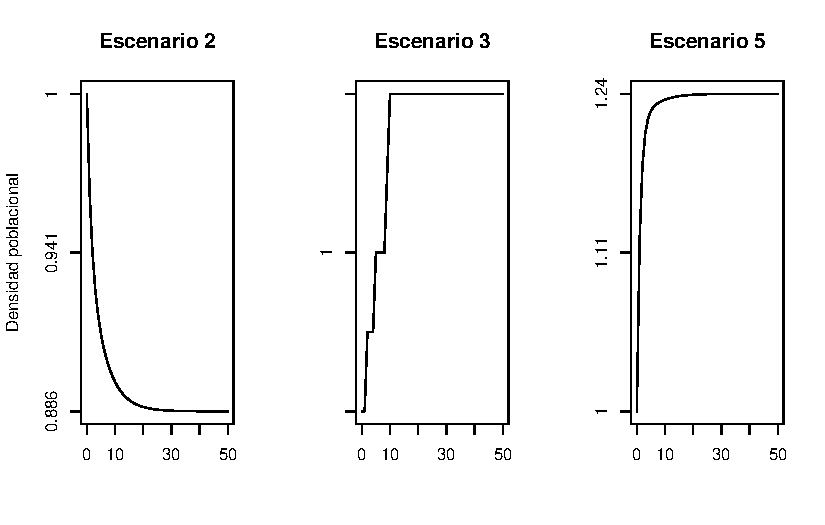
\includegraphics[keepaspectratio]{112-Dinamica_de_Transiciones_files/figure-pdf/trans14-1.pdf}}

\begin{center}\rule{0.5\linewidth}{0.5pt}\end{center}

\section{Gráfica de la dinámica poblacional transitoria
estandarizada}\label{gruxe1fica-de-la-dinuxe1mica-poblacional-transitoria-estandarizada}

En el siguiente recuadro se integran en una sola gráfica los resultados
de la dinámica poblacional transitoria estandarizada de \emph{L.
rubripetala} para los escenarios 1, 3 y 5.

\pandocbounded{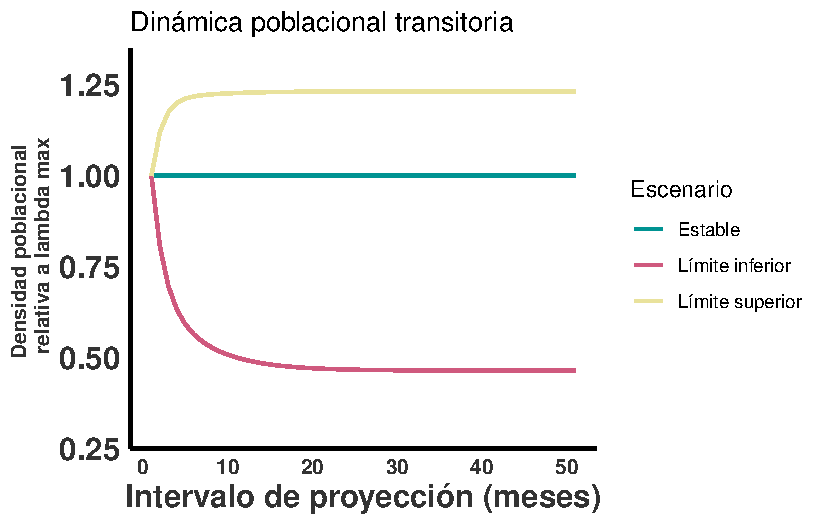
\includegraphics[keepaspectratio]{112-Dinamica_de_Transiciones_files/figure-pdf/trans15-1.pdf}}

La gráfica a continuación corresponde a los cinco escenarios planteados
para la población 1 de \emph{L. rubripetala}, semejante a la figura 2B
del artículo de Tremblay y colaboradores (Tremblay, Raventos \&
Ackerman, 2015); aunque cabe señalar que no se integran los índices
transitorios, los cuales abordamos a continuación.

\begin{center}\rule{0.5\linewidth}{0.5pt}\end{center}

\subsection{Índices transitorios}\label{uxedndices-transitorios}

Se determinan los \emph{límites de la dinámica transitoria} con el fin
de evaluar en el corto plazo los cambios cuantitativos en la población,
debido a perturbaciones repentinas en la estructura poblacional. Estos
se calculan en los modelos a corto plazo a través de los \emph{Índices
de transferencia} (Stott, Townley \& Hodgson, 2011), los cuales se
estiman previo a que se alcance la tasa constante de crecimiento
poblacional e incluyen los siguientes tres parámetros:

\emph{i}) \emph{Reactividad alta y Reactividad baja} (Upper reactivity y
Lower reactivity) que representan el crecimiento o el decremento
inmediato (i.e.~primer intervalo de tiempo).

\emph{ii}) \emph{Máxima amplificación y Máxima atenuación} (Maximum
amplification y Maximum attenuation) que indican, respectivamente, el
incremento o decremento máximo futuro del crecimiento poblacional.

\emph{iii}) \emph{Inercia alta e Inercia baja} (Upper inertia y Lower
inertia) que evalúan el límite más alto o el más bajo en el crecimiento
de la población.

\begin{tcolorbox}[enhanced jigsaw, arc=.35mm, bottomrule=.15mm, bottomtitle=1mm, breakable, colback=white, colbacktitle=quarto-callout-note-color!10!white, colframe=quarto-callout-note-color-frame, coltitle=black, left=2mm, leftrule=.75mm, opacityback=0, opacitybacktitle=0.6, rightrule=.15mm, title=\textcolor{quarto-callout-note-color}{\faInfo}\hspace{0.5em}{Nota}, titlerule=0mm, toprule=.15mm, toptitle=1mm]

\textbf{Tres índices que resumen la dinámica transitoria.}

{\def\LTcaptype{none} % do not increment counter
\begin{longtable}[]{@{}
  >{\raggedright\arraybackslash}p{(\linewidth - 4\tabcolsep) * \real{0.3333}}
  >{\raggedright\arraybackslash}p{(\linewidth - 4\tabcolsep) * \real{0.3333}}
  >{\raggedright\arraybackslash}p{(\linewidth - 4\tabcolsep) * \real{0.3333}}@{}}
\toprule\noalign{}
\begin{minipage}[b]{\linewidth}\raggedright
Índice
\end{minipage} & \begin{minipage}[b]{\linewidth}\raggedright
Qué mide
\end{minipage} & \begin{minipage}[b]{\linewidth}\raggedright
Cuándo es útil
\end{minipage} \\
\midrule\noalign{}
\endhead
\bottomrule\noalign{}
\endlastfoot
\textbf{Reactividad} (\texttt{reac}) & Cambio inmediato (primer paso) en
el tamaño relativo de la población. & Para evaluar la respuesta inicial
a una perturbación. \\
\textbf{Máxima amplificación / atenuación} (\texttt{maxamp},
\texttt{maxatt}) & El máximo crecimiento o decremento alcanzado durante
la transición. & Para identificar el escenario de ``auge'' o ``declive
temporal'' más extremo. \\
\textbf{Inercia} (\texttt{inertia}) & Diferencia a largo plazo entre el
escenario transitorio y la trayectoria asintótica. & Para cuantificar el
``legado'' permanente de la estructura inicial sobre el tamaño
futuro. \\
\end{longtable}
}

Cada uno tiene una variante ``alta'' (\emph{upper}) y ``baja''
(\emph{lower}), correspondiente a estructuras iniciales que producen el
máximo o mínimo del índice respectivamente.

\end{tcolorbox}

\subsubsection{Cálculo de los límites
transitorios}\label{cuxe1lculo-de-los-luxedmites-transitorios}

\begin{itemize}
\tightlist
\item
  Escenario 1 (límite inferior):
\end{itemize}

\begin{Shaded}
\begin{Highlighting}[]
\CommentTok{\#Escenario 1 (límite inferior):}
\NormalTok{lim.trans }\OtherTok{\textless{}{-}} \FunctionTok{as.data.frame}\NormalTok{(}\FunctionTok{matrix}\NormalTok{(}\ConstantTok{NA}\NormalTok{, }\DecValTok{5}\NormalTok{, }\DecValTok{3}\NormalTok{))}
\FunctionTok{names}\NormalTok{(lim.trans) }\OtherTok{\textless{}{-}} \FunctionTok{c}\NormalTok{(}\StringTok{"reac"}\NormalTok{, }\StringTok{"maxatt"}\NormalTok{, }\StringTok{"inertia"}\NormalTok{)}

\NormalTok{reac1 }\OtherTok{\textless{}{-}} \FunctionTok{reac}\NormalTok{(Lr1, }\AttributeTok{vector =}\NormalTok{ nLr1)}
\NormalTok{lim.trans[}\DecValTok{1}\NormalTok{, }\DecValTok{1}\NormalTok{] }\OtherTok{\textless{}{-}}\NormalTok{ reac1}
\NormalTok{reac1}
\end{Highlighting}
\end{Shaded}

\begin{verbatim}
[1] 0.8055011
\end{verbatim}

\begin{Shaded}
\begin{Highlighting}[]
\NormalTok{maxatt1 }\OtherTok{\textless{}{-}} \FunctionTok{maxatt}\NormalTok{(Lr1, }\AttributeTok{vector =}\NormalTok{ nLr1, }\AttributeTok{return.t =}\NormalTok{ T)}
\NormalTok{maxatt1}
\end{Highlighting}
\end{Shaded}

\begin{verbatim}
$maxatt
[1] 0.4646221

$t
[1] 49
\end{verbatim}

\begin{Shaded}
\begin{Highlighting}[]
\NormalTok{lim.trans[}\DecValTok{1}\NormalTok{, }\DecValTok{2}\NormalTok{] }\OtherTok{\textless{}{-}}\NormalTok{ maxatt1[}\DecValTok{1}\NormalTok{]}

\NormalTok{inertia1 }\OtherTok{\textless{}{-}} \FunctionTok{inertia}\NormalTok{(Lr1, }\AttributeTok{vector =}\NormalTok{ nLr1)}
\NormalTok{inertia1}
\end{Highlighting}
\end{Shaded}

\begin{verbatim}
[1] 0.4646004
\end{verbatim}

\begin{Shaded}
\begin{Highlighting}[]
\NormalTok{lim.trans[}\DecValTok{1}\NormalTok{, }\DecValTok{3}\NormalTok{] }\OtherTok{\textless{}{-}}\NormalTok{ inertia1}
\end{Highlighting}
\end{Shaded}

\begin{center}\rule{0.5\linewidth}{0.5pt}\end{center}

\begin{itemize}
\tightlist
\item
  Escenario 3 (estructura estable):
\end{itemize}

\begin{Shaded}
\begin{Highlighting}[]
\CommentTok{\#Escenario 3 (estructura estable):}
\NormalTok{reac3 }\OtherTok{\textless{}{-}} \FunctionTok{reac}\NormalTok{(Lr1, }\AttributeTok{vector =}\NormalTok{ nLr3)}
\NormalTok{lim.trans[}\DecValTok{3}\NormalTok{, }\DecValTok{1}\NormalTok{] }\OtherTok{\textless{}{-}}\NormalTok{ reac3}
\NormalTok{reac3}
\end{Highlighting}
\end{Shaded}

\begin{verbatim}
[1] 1
\end{verbatim}

\begin{Shaded}
\begin{Highlighting}[]
\NormalTok{inertia3 }\OtherTok{\textless{}{-}} \FunctionTok{inertia}\NormalTok{(Lr1, }\AttributeTok{vector =}\NormalTok{ nLr3)}
\NormalTok{inertia3}
\end{Highlighting}
\end{Shaded}

\begin{verbatim}
[1] 1
\end{verbatim}

\begin{Shaded}
\begin{Highlighting}[]
\NormalTok{lim.trans[}\DecValTok{3}\NormalTok{, }\DecValTok{3}\NormalTok{] }\OtherTok{\textless{}{-}}\NormalTok{ inertia3}
\end{Highlighting}
\end{Shaded}

\begin{center}\rule{0.5\linewidth}{0.5pt}\end{center}

\begin{itemize}
\tightlist
\item
  Escenario 5 (límite superior):
\end{itemize}

\begin{Shaded}
\begin{Highlighting}[]
\CommentTok{\#Escenario 5. Límite superior}
\NormalTok{reac5 }\OtherTok{\textless{}{-}} \FunctionTok{reac}\NormalTok{(Lr1, }\AttributeTok{vector =}\NormalTok{ nLr5)}
\NormalTok{lim.trans[}\DecValTok{5}\NormalTok{, }\DecValTok{1}\NormalTok{] }\OtherTok{\textless{}{-}}\NormalTok{ reac5}
\NormalTok{reac5}
\end{Highlighting}
\end{Shaded}

\begin{verbatim}
[1] 1.119635
\end{verbatim}

\begin{Shaded}
\begin{Highlighting}[]
\NormalTok{maxamp5 }\OtherTok{\textless{}{-}} \FunctionTok{maxamp}\NormalTok{(Lr1, }\AttributeTok{vector =}\NormalTok{ nLr5, }\AttributeTok{return.t =}\NormalTok{ T, }\AttributeTok{conv.accuracy =} \FloatTok{0.01}\NormalTok{)}
\NormalTok{maxamp5}
\end{Highlighting}
\end{Shaded}

\begin{verbatim}
$maxamp
[1] 1.211761

$t
[1] 4
\end{verbatim}

\begin{Shaded}
\begin{Highlighting}[]
\NormalTok{lim.trans[}\DecValTok{5}\NormalTok{, }\DecValTok{2}\NormalTok{] }\OtherTok{\textless{}{-}}\NormalTok{ maxamp5[}\DecValTok{1}\NormalTok{]}
\NormalTok{inertia5 }\OtherTok{\textless{}{-}} \FunctionTok{inertia}\NormalTok{(Lr1, }\AttributeTok{vector =}\NormalTok{ nLr5)}
\NormalTok{inertia5}
\end{Highlighting}
\end{Shaded}

\begin{verbatim}
[1] 1.231728
\end{verbatim}

\begin{Shaded}
\begin{Highlighting}[]
\NormalTok{lim.trans[}\DecValTok{5}\NormalTok{, }\DecValTok{3}\NormalTok{] }\OtherTok{\textless{}{-}}\NormalTok{ inertia5}
\end{Highlighting}
\end{Shaded}

\subsubsection{Crear una tabla de los índices
transitorios}\label{crear-una-tabla-de-los-uxedndices-transitorios}

\begin{Shaded}
\begin{Highlighting}[]
\CommentTok{\#Escenario 2 (inicio I):}
\NormalTok{reac2 }\OtherTok{\textless{}{-}} \FunctionTok{reac}\NormalTok{(Lr1, }\AttributeTok{vector =}\NormalTok{ nLr2)}
\NormalTok{reac2}
\NormalTok{lim.trans[}\DecValTok{2}\NormalTok{, }\DecValTok{1}\NormalTok{] }\OtherTok{\textless{}{-}}\NormalTok{ reac2}
\NormalTok{maxatt2 }\OtherTok{\textless{}{-}} \FunctionTok{maxatt}\NormalTok{(Lr1, }\AttributeTok{vector =}\NormalTok{ nLr2, }\AttributeTok{return.t =}\NormalTok{ T)}
\NormalTok{maxatt2}
\NormalTok{lim.trans[}\DecValTok{2}\NormalTok{, }\DecValTok{2}\NormalTok{] }\OtherTok{\textless{}{-}}\NormalTok{ maxatt2[}\DecValTok{1}\NormalTok{]}
\NormalTok{inertia2 }\OtherTok{\textless{}{-}} \FunctionTok{inertia}\NormalTok{(Lr1, }\AttributeTok{vector =}\NormalTok{ nLr2)}
\NormalTok{inertia2}
\NormalTok{lim.trans[}\DecValTok{2}\NormalTok{, }\DecValTok{3}\NormalTok{] }\OtherTok{\textless{}{-}}\NormalTok{ inertia2}

\CommentTok{\#Escenario 4. Inicio II}
\NormalTok{reac4 }\OtherTok{\textless{}{-}} \FunctionTok{reac}\NormalTok{(Lr1, }\AttributeTok{vector =}\NormalTok{ nLr4)}
\NormalTok{lim.trans[}\DecValTok{4}\NormalTok{, }\DecValTok{1}\NormalTok{] }\OtherTok{\textless{}{-}}\NormalTok{ reac4}
\NormalTok{reac4}
\NormalTok{maxatt4 }\OtherTok{\textless{}{-}} \FunctionTok{maxatt}\NormalTok{(Lr1, }\AttributeTok{vector =}\NormalTok{ nLr4, }\AttributeTok{return.t =}\NormalTok{ T)}
\NormalTok{maxatt4}
\NormalTok{lim.trans[}\DecValTok{4}\NormalTok{, }\DecValTok{2}\NormalTok{] }\OtherTok{\textless{}{-}}\NormalTok{ maxatt4[}\DecValTok{1}\NormalTok{]}
\NormalTok{inertia4 }\OtherTok{\textless{}{-}} \FunctionTok{inertia}\NormalTok{(Lr1, }\AttributeTok{vector =}\NormalTok{ nLr4)}
\NormalTok{inertia4}
\NormalTok{lim.trans[}\DecValTok{4}\NormalTok{, }\DecValTok{3}\NormalTok{] }\OtherTok{\textless{}{-}}\NormalTok{ inertia4}
\end{Highlighting}
\end{Shaded}

\begin{center}\rule{0.5\linewidth}{0.5pt}\end{center}

\subsection{Tabla de los índices
transitorios}\label{tabla-de-los-uxedndices-transitorios}

En la tabla del siguiente recuadro se resumen los valores estimados por
escenario.

\begin{Shaded}
\begin{Highlighting}[]
\FunctionTok{flextable}\NormalTok{(lim.trans)}
\end{Highlighting}
\end{Shaded}

\global\setlength{\Oldarrayrulewidth}{\arrayrulewidth}

\global\setlength{\Oldtabcolsep}{\tabcolsep}

\setlength{\tabcolsep}{2pt}

\renewcommand*{\arraystretch}{1.5}



\providecommand{\ascline}[3]{\noalign{\global\arrayrulewidth #1}\arrayrulecolor[HTML]{#2}\cline{#3}}

\begin{longtable*}[c]{ccc}



\ascline{1.5pt}{666666}{1-3}

\multicolumn{1}{>{}r}{\textcolor[HTML]{000000}{\fontsize{11}{11}\selectfont{reac}}} & \multicolumn{1}{>{}r}{\textcolor[HTML]{000000}{\fontsize{11}{11}\selectfont{maxatt}}} & \multicolumn{1}{>{}r}{\textcolor[HTML]{000000}{\fontsize{11}{11}\selectfont{inertia}}} \\

\ascline{1.5pt}{666666}{1-3}\endfirsthead 

\ascline{1.5pt}{666666}{1-3}

\multicolumn{1}{>{}r}{\textcolor[HTML]{000000}{\fontsize{11}{11}\selectfont{reac}}} & \multicolumn{1}{>{}r}{\textcolor[HTML]{000000}{\fontsize{11}{11}\selectfont{maxatt}}} & \multicolumn{1}{>{}r}{\textcolor[HTML]{000000}{\fontsize{11}{11}\selectfont{inertia}}} \\

\ascline{1.5pt}{666666}{1-3}\endhead



\multicolumn{1}{>{}r}{\textcolor[HTML]{000000}{\fontsize{11}{11}\selectfont{0.8055011}}} & \multicolumn{1}{>{}r}{\textcolor[HTML]{000000}{\fontsize{11}{11}\selectfont{0.4646221}}} & \multicolumn{1}{>{}r}{\textcolor[HTML]{000000}{\fontsize{11}{11}\selectfont{0.4646004}}} \\





\multicolumn{1}{>{}r}{\textcolor[HTML]{000000}{\fontsize{11}{11}\selectfont{0.9626875}}} & \multicolumn{1}{>{}r}{\textcolor[HTML]{000000}{\fontsize{11}{11}\selectfont{0.8846214}}} & \multicolumn{1}{>{}r}{\textcolor[HTML]{000000}{\fontsize{11}{11}\selectfont{0.8845797}}} \\





\multicolumn{1}{>{}r}{\textcolor[HTML]{000000}{\fontsize{11}{11}\selectfont{1.0000000}}} & \multicolumn{1}{>{}r}{\textcolor[HTML]{000000}{\fontsize{11}{11}\selectfont{}}} & \multicolumn{1}{>{}r}{\textcolor[HTML]{000000}{\fontsize{11}{11}\selectfont{1.0000000}}} \\





\multicolumn{1}{>{}r}{\textcolor[HTML]{000000}{\fontsize{11}{11}\selectfont{0.9271806}}} & \multicolumn{1}{>{}r}{\textcolor[HTML]{000000}{\fontsize{11}{11}\selectfont{0.7879760}}} & \multicolumn{1}{>{}r}{\textcolor[HTML]{000000}{\fontsize{11}{11}\selectfont{0.7879393}}} \\





\multicolumn{1}{>{}r}{\textcolor[HTML]{000000}{\fontsize{11}{11}\selectfont{1.1196345}}} & \multicolumn{1}{>{}r}{\textcolor[HTML]{000000}{\fontsize{11}{11}\selectfont{1.2117612}}} & \multicolumn{1}{>{}r}{\textcolor[HTML]{000000}{\fontsize{11}{11}\selectfont{1.2317285}}} \\

\ascline{1.5pt}{666666}{1-3}



\end{longtable*}



\arrayrulecolor[HTML]{000000}

\global\setlength{\arrayrulewidth}{\Oldarrayrulewidth}

\global\setlength{\tabcolsep}{\Oldtabcolsep}

\renewcommand*{\arraystretch}{1}

\begin{center}\rule{0.5\linewidth}{0.5pt}\end{center}

\section{Gráfica de dinámica poblacional transitoria integrando los
índices transitorios: escenarios 1, 3 y
5.}\label{gruxe1fica-de-dinuxe1mica-poblacional-transitoria-integrando-los-uxedndices-transitorios-escenarios-1-3-y-5.}

En el siguiente recuadro se integran en una sola gráfica los resultados
de la dinámica transitoria estandarizada de \emph{L. rubripetala} para
los escenarios 1, 3 y 5.

\begin{Shaded}
\begin{Highlighting}[]
\NormalTok{len }\OtherTok{\textless{}{-}} \FunctionTok{nrow}\NormalTok{(pr2}\FloatTok{.1}\NormalTok{)}
\NormalTok{Population\_density }\OtherTok{\textless{}{-}} \FunctionTok{rbind}\NormalTok{(}
  \FunctionTok{data.frame}\NormalTok{(}\AttributeTok{Projection =}\NormalTok{ pr2}\FloatTok{.1}\NormalTok{, }\AttributeTok{Escenario =} \StringTok{"Límite inferior"}\NormalTok{),}
  \FunctionTok{data.frame}\NormalTok{(}\AttributeTok{Projection =}\NormalTok{ pr2}\FloatTok{.3}\NormalTok{, }\AttributeTok{Escenario =} \StringTok{"Estable"}\NormalTok{),}
  \FunctionTok{data.frame}\NormalTok{(}\AttributeTok{Projection =}\NormalTok{ pr2}\FloatTok{.5}\NormalTok{, }\AttributeTok{Escenario =} \StringTok{"Límite superior"}\NormalTok{)}
\NormalTok{)}
\NormalTok{Population\_density}\SpecialCharTok{$}\NormalTok{Time }\OtherTok{\textless{}{-}} \FunctionTok{rep}\NormalTok{(}\FunctionTok{seq}\NormalTok{(}\DecValTok{1}\NormalTok{, len, }\DecValTok{1}\NormalTok{), }\DecValTok{3}\NormalTok{)}

\NormalTok{trans.plot }\OtherTok{\textless{}{-}} \FunctionTok{ggplot}\NormalTok{(}\AttributeTok{data =}\NormalTok{ Population\_density) }\SpecialCharTok{+}
  \FunctionTok{theme\_minimal}\NormalTok{() }\SpecialCharTok{+}
  \CommentTok{\# theme(panel.border = element\_blank()) +}
  \CommentTok{\#theme(legend.position = "none") +}
  \FunctionTok{geom\_line}\NormalTok{(}
    \FunctionTok{aes}\NormalTok{(}\AttributeTok{x =}\NormalTok{ Time, }\AttributeTok{y =}\NormalTok{ Projection, }\AttributeTok{group =}\NormalTok{ Escenario, }\AttributeTok{colour =}\NormalTok{ Escenario),}
    \AttributeTok{linewidth =} \FloatTok{0.8}
\NormalTok{  ) }\SpecialCharTok{+}
  \FunctionTok{scale\_colour\_manual}\NormalTok{(}\AttributeTok{values =} \FunctionTok{c}\NormalTok{(}\StringTok{"green4"}\NormalTok{, }\StringTok{"black"}\NormalTok{, }\StringTok{"orange2"}\NormalTok{)) }\SpecialCharTok{+}
  \FunctionTok{labs}\NormalTok{(}
    \AttributeTok{title =} \StringTok{"Dinámica poblacional transitoria"}\NormalTok{,}
    \AttributeTok{x =} \StringTok{"Intervalo de proyección (meses)"}\NormalTok{,}
    \AttributeTok{y =} \StringTok{"Densidad poblacional relativa }\SpecialCharTok{\textbackslash{}n}\StringTok{ a lambda max"}
\NormalTok{  ) }\SpecialCharTok{+}
  \FunctionTok{ylim}\NormalTok{(}\FloatTok{0.3}\NormalTok{, }\FloatTok{1.3}\NormalTok{) }\SpecialCharTok{+}
  \FunctionTok{rlt\_style\_colour}\NormalTok{()}

\NormalTok{trans.plot }\SpecialCharTok{+}
  \FunctionTok{annotate}\NormalTok{(}
    \StringTok{"text"}\NormalTok{,}
    \AttributeTok{x =} \DecValTok{49}\NormalTok{,}
    \AttributeTok{y =}\NormalTok{ maxatt1}\SpecialCharTok{$}\NormalTok{maxatt,}
    \CommentTok{\# 1. Change expression() to a string}
    \CommentTok{\# 2. Add parse = TRUE}
    \AttributeTok{label =} \StringTok{"underline(rho) == 0.46"}\NormalTok{,}
    \AttributeTok{parse =} \ConstantTok{TRUE}\NormalTok{,}
    \AttributeTok{hjust =} \FloatTok{1.0}\NormalTok{,}
    \AttributeTok{vjust =} \SpecialCharTok{{-}}\DecValTok{1}
\NormalTok{  ) }\SpecialCharTok{+}
  \FunctionTok{annotate}\NormalTok{(}
    \StringTok{"text"}\NormalTok{,}
    \AttributeTok{x =} \DecValTok{49}\NormalTok{,}
    \AttributeTok{y =}\NormalTok{ maxamp5}\SpecialCharTok{$}\NormalTok{maxamp,}
    \CommentTok{\# 1. Change expression() to a string}
    \CommentTok{\# 2. Add parse = TRUE}
    \AttributeTok{label =} \StringTok{"bar(rho) == 1"}\NormalTok{,}
    \AttributeTok{parse =} \ConstantTok{TRUE}\NormalTok{,}
    \AttributeTok{hjust =} \FloatTok{1.22}\NormalTok{,}
    \AttributeTok{vjust =} \SpecialCharTok{{-}}\DecValTok{1}
\NormalTok{  )}
\end{Highlighting}
\end{Shaded}

\pandocbounded{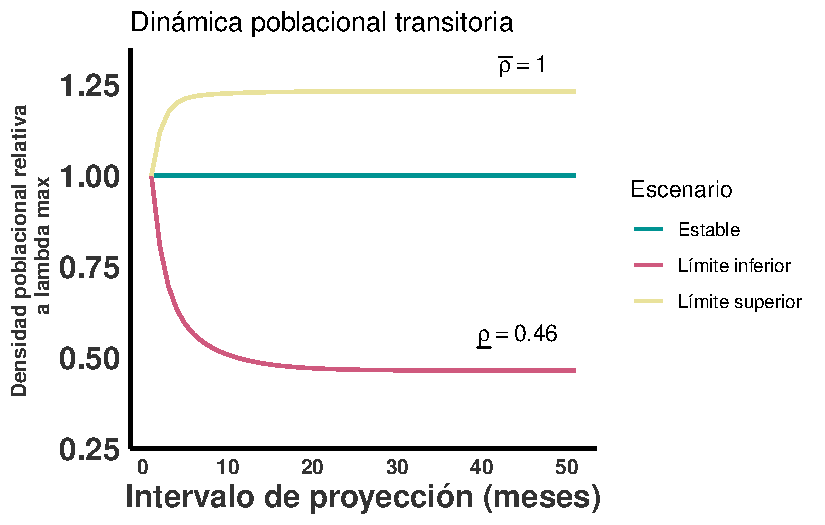
\includegraphics[keepaspectratio]{112-Dinamica_de_Transiciones_files/figure-pdf/trans22-1.pdf}}

\begin{center}\rule{0.5\linewidth}{0.5pt}\end{center}

La gráfica a continuación corresponde a los cinco escenarios planteados
para la población 1 de \emph{L. rubripetala}, equivalente a la figura 2B
del artículo de Tremblay y colaboradores ((Tremblay, Raventos \&
Ackerman, 2015)). Esta permitirá comparar tus resultados y verificar que
los escenarios que has desarrollado estén correctos.

\pandocbounded{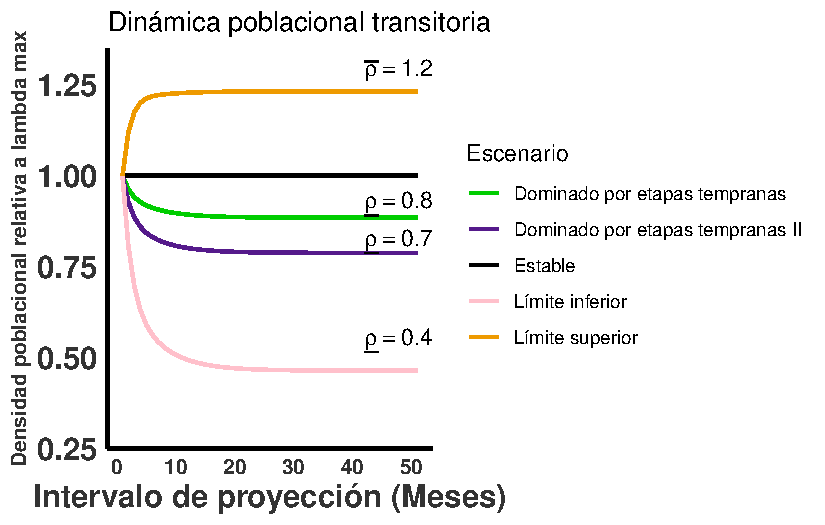
\includegraphics[keepaspectratio]{112-Dinamica_de_Transiciones_files/figure-pdf/trans23-1.pdf}}

\bookmarksetup{startatroot}

\chapter{Funciones de transferencia}\label{funciones-de-transferencia}

Por: Mariana Hernández-Apolinar, Tamara Ticktin, Edgar J. González y
Raymond L. Tremblay

Las funciones de transferencia describen cómo los cambios en una
variable o estado demográfico se traducen en respuestas a otra escala
del sistema. Este capítulo introduce las funciones de transferencia como
herramientas conceptuales que vinculan los procesos, los estados del
ciclo de vida y las respuestas poblacionales.

\section{Funciones de transferencia y relaciones entre procesos
demográficos}\label{funciones-de-transferencia-y-relaciones-entre-procesos-demogruxe1ficos}

En el contexto de la dinámica de poblaciones, las funciones de
transferencia son herramientas de análisis que permiten describir y
formalizar la relación entre los cambios en las variables demográficas y
sus efectos sobre otros componentes del sistema. Estas funciones
describen cómo variaciones en los procesos individuales, las condiciones
ambientales o los estados del ciclo de vida se traducen en cambios en la
estructura demográfica de la población.

En este capítulo se presenta el papel de las funciones de transferencia
como herramientas que permiten traducir información entre escalas y
procesos dentro de los modelos poblacionales. Se discute cómo estas
funciones pueden representar relaciones no lineales, umbrales o
dependencias funcionales entre variables, y cómo su elección influye en
la dinámica resultante del sistema.

A diferencia de los capítulos sobre simulaciones o análisis
retrospectivos, este capítulo no se centra en proyectar trayectorias
poblacionales completas, sino en comprender \textbf{cómo} las
modificaciones en un componente específico del sistema se transfieren a
otros componentes. Las funciones de transferencia son herramientas que
permiten integrar y traducir información entre distintas escalas y
procesos en los modelos poblacionales, y son especialmente útiles para
integrar los procesos biológicos, las covariables ambientales y los
supuestos de manejo en modelos dinámicos más realistas. Las funciones de
transferencia se construyen a partir de los procesos demográficos
descritos en el capítulo de \hyperref[MatricesT]{Transiciones}. Las
funciones de transferencia permiten incorporar mecanismos específicos en
las simulaciones poblacionales descritas en el capítulo de
\href{115-Metodos_de_simulaciones.qmd}{Métodos de simulaciones}.

\section{Definición e implementación de funciones de
transferencia}\label{definiciuxf3n-e-implementaciuxf3n-de-funciones-de-transferencia}

A continuación se describen distintos tipos de funciones de
transferencia y su implementación en modelos de dinámica poblacional.

\subsubsection{Librerías de R requeridas para el siguiente
módulo}\label{libreruxedas-de-r-requeridas-para-el-siguiente-muxf3dulo-10}

\begin{Shaded}
\begin{Highlighting}[]
\FunctionTok{library}\NormalTok{(popdemo)}
\FunctionTok{library}\NormalTok{(tidyverse)}
\FunctionTok{library}\NormalTok{(cowplot)}
\end{Highlighting}
\end{Shaded}

\section{Dinámica transitoria y funciones de
transferencia}\label{dinuxe1mica-transitoria-y-funciones-de-transferencia}

Los modelos de dinámica transitoria constituyen una alternativa para
analizar la evolución de una población ante eventos de perturbación
repentinos, ya sean de origen biótico (por ejemplo, depredación),
abiótico (por ejemplo, huracanes) o antropogénico (por ejemplo,
extracción) (Ezard et~al., 2010). En el capítulo dedicado a la
\hyperref[Dinamica_transitoria]{dinámica transitoria} aprendimos a
evaluar la respuesta inmediata o de corto plazo del crecimiento
poblacional (\(\lambda_{\max}\)) frente a la alteración de la estructura
poblacional. Asimismo, mediante los índices de transferencia comparamos
los cambios en la densidad poblacional cuando la estructura no se
encuentra en una distribución estable, variando la proporción de
individuos por categoría (por ejemplo, solo semillas o únicamente
individuos adultos).

Continuando con los análisis de la dinámica transitoria de \emph{L.
rubripetala} realizados por Tremblay y colaboradores (Tremblay, Raventos
\& Ackerman, 2015), en este capítulo abordaremos los análisis de
perturbación transitoria. Estos permiten proyectar cómo responde la
dinámica poblacional transitoria ante la manipulación de las tasas
vitales (supervivencia, reproducción y crecimiento) y de la estructura
poblacional (abundancia relativa de individuos de diferentes edades,
tamaños o estados) (Stott, 2016). Dichos análisis son herramientas clave
para identificar qué individuos o tasas vitales son más relevantes para
la dinámica a corto plazo. A partir de estos resultados, es posible
definir estrategias de conservación y manejo más eficientes, que
permitan alcanzar tasas de crecimiento planificadas para la especie de
interés (\(\lambda = 1\), \(\lambda < 1\) o \(\lambda > 1\)), con el
mínimo esfuerzo o costo (Stott, 2016).

En el modelo de crecimiento asintótico o de largo plazo, tratado en el
capítulo de \hyperref[Elasticidad]{Elasticidad}, se realizaron dos
análisis de perturbación: sensibilidad y elasticidad, que estiman los
efectos absolutos y relativos, respectivamente, de pequeñas
perturbaciones sobre la tasa de crecimiento poblacional (\(\lambda\))
(Caswell, 2001). Sin embargo, estos análisis no son adecuados para
evaluar la dinámica a corto plazo, ya que resultan poco eficientes para
describir la respuesta poblacional ante perturbaciones de gran magnitud
(Stott, Townley \& Hodgson, 2011; Stott, Hodgson \& Townley, 2012a).
Además, dichos análisis asumen una relación lineal entre la perturbación
y el crecimiento poblacional en modelos asintóticos, lo cual no refleja
la respuesta no lineal característica de los modelos de dinámica
transitoria (Stott, Townley \& Hodgson, 2011; Stott, Hodgson \& Townley,
2012a).

Dado que algunas poblaciones están sujetas a perturbaciones repentinas o
intensas en ciertos periodos, su comportamiento poblacional puede ser
altamente variable (Bierzychudek, 1999; Hastings, 2001). Por ello,
existe un interés creciente en evaluar cuantitativamente la sensibilidad
y la elasticidad no lineal (Stott, Hodgson \& Townley, 2012a; Stott,
2016). Entre los métodos desarrollados para este fin, en este capítulo
abordaremos el análisis de la función de transferencia aplicado a
matrices de proyección poblacional.

\subsection{Análisis de elasticidad: lineales y no
lineales}\label{anuxe1lisis-de-elasticidad-lineales-y-no-lineales}

Es importante destacar que los análisis de perturbación a largo plazo
(De Kroon, Van Groenendael \& Ehrlén, 2000; Caswell, 2001), explicados
en el capítulo de \hyperref[Elasticidad]{Elasticidad}, suponen que la
tasa de crecimiento poblacional (\(\lambda\)) varía de manera lineal
cuando se modifica algún elemento de la dinámica poblacional. Esto
implica que un cambio en un componente del sistema se traduce en un
cambio proporcional en la tasa de crecimiento. Esta suposición es válida
cuando las perturbaciones son pequeñas, ya que el efecto sobre
\(\lambda\) será igualmente reducido.

Sin embargo, cuando las perturbaciones son grandes, los efectos no
necesariamente siguen un patrón lineal (Bialic-Murphy, Gaoue \& Knight,
2018). En tales casos, los resultados derivados de los análisis
tradicionales pueden ser subóptimos, llegando a subestimar o
sobreestimar la importancia absoluta o relativa de las tasas vitales o
de las categorías de la variable de estado sobre la tasa de crecimiento
poblacional.

Por el contrario, los análisis de perturbación transitorios no
presuponen este comportamiento lineal, lo que los hace más adecuados
para evaluar la respuesta de una población ante eventos de perturbación
de gran magnitud (Hodgson \& Townley, 2004). Estos análisis permiten
capturar la complejidad y la naturaleza no lineal de la dinámica
transitoria, ofreciendo una visión más realista del comportamiento
poblacional en escenarios de cambio abrupto.

\begin{tcolorbox}[enhanced jigsaw, arc=.35mm, bottomrule=.15mm, bottomtitle=1mm, breakable, colback=white, colbacktitle=quarto-callout-important-color!10!white, colframe=quarto-callout-important-color-frame, coltitle=black, left=2mm, leftrule=.75mm, opacityback=0, opacitybacktitle=0.6, rightrule=.15mm, title=\textcolor{quarto-callout-important-color}{\faExclamation}\hspace{0.5em}{Importante}, titlerule=0mm, toprule=.15mm, toptitle=1mm]

\textbf{La elasticidad clásica supone linealidad --- y esa suposición se
rompe con perturbaciones grandes.} Sensibilidad y elasticidad asumen que
un cambio del 10\% en una entrada produce el doble del efecto que un
cambio del 5\%. Esta suposición se cumple bien para perturbaciones
pequeñas (≲ 1--2\%), pero para cambios grandes (e.g., reducir mortalidad
adulta a la mitad, eliminar reproducción de un estadio) la respuesta de
λ es típicamente \textbf{no lineal}. Las funciones de transferencia
calculan la respuesta exacta de λ para cualquier magnitud de
perturbación, sin asumir linealidad.

\end{tcolorbox}

\begin{center}\rule{0.5\linewidth}{0.5pt}\end{center}

\subsection{Análisis de perturbación: elasticidad en la dinámica
poblacional
transitoria}\label{anuxe1lisis-de-perturbaciuxf3n-elasticidad-en-la-dinuxe1mica-poblacional-transitoria}

Los análisis de perturbación aplicados a la dinámica poblacional
transitoria se han desarrollado desde tres enfoques principales:
diferenciación, perturbación directa y función de transferencia (Stott,
2016). En particular, Tremblay y colaboradores emplearon el enfoque
basado en la función de transferencia para calcular la elasticidad no
lineal (Tremblay, Raventos \& Ackerman, 2015).

Este método fue incorporado al análisis poblacional por Hodgson y
Townley en 2004 (Hodgson \& Townley, 2004), adaptándolo del campo del
control robusto de sistemas. Su aplicación en matrices de proyección
poblacional ha demostrado ser altamente útil, ya que proporciona un
marco sólido para determinar relaciones no lineales exactas entre
perturbaciones en las tasas vitales y los cambios resultantes en la
densidad y el crecimiento poblacional (Hodgson \& Townley, 2004; Stott,
2016).

Además, la función de transferencia permite estimar cuantitativamente
tanto la magnitud como el patrón temporal de la respuesta poblacional
frente a distintos tipos de perturbaciones. Esta relación suele ser
compleja y difícil de proyectar mediante otros métodos de análisis
transitorio (Stott, 2016).

\subsection{Marco de análisis de las funciones de
transferencia}\label{marco-de-anuxe1lisis-de-las-funciones-de-transferencia}

A continuación se presenta una descripción general de los componentes
que integran el marco de análisis para la elasticidad no lineal basada
en funciones de transferencia, junto con las ecuaciones más relevantes
utilizadas en el cálculo de estos parámetros. Para una explicación más
detallada, se recomienda consultar los trabajos de Hodgson y Townley,
así como los de Stott y colaboradores (Hodgson \& Townley, 2004; Stott,
Hodgson \& Townley, 2012a). El análisis de elasticidad no lineal
mediante la función de transferencia incorpora los siguientes elementos:

\begin{itemize}
\tightlist
\item
  La matriz de proyección poblacional (MPP), denotada como \(A\), que
  describe el ciclo de vida de la población en estudio.
\item
  Los elementos de la matriz, definidos como la estructura de
  perturbación,
\item
  La magnitud con la que se altera una estructura de perturbación,
  representada por \(\delta\).
\item
  La ubicación de dichos elementos, determinada por los vectores \(d\)
  (columna) y \(e\) (renglón).
\end{itemize}

Al combinar estos componentes mediante multiplicaciones y sumas según la
ecuación correspondiente, se obtiene una matriz que indica qué elementos
han sido perturbados. En esta ecuación, \(e^T\) representa la
transposición del vector \(e\), convirtiéndolo de columna a renglón.
Este procedimiento permite estimar el efecto de una perturbación sobre
la tasa de crecimiento poblacional a largo plazo (Stott, Hodgson \&
Townley, 2012a).

\[A_{\delta}= A + \delta de^T\]

En esta ecuación, la matriz \(A\) presenta propiedades emergentes, lo
que implica un crecimiento asintótico o de largo plazo definido por
\(\lambda_{max}\), acompañado de un eigenvector derecho (\(w\),
estructura estable) y un eigenvector izquierdo (\(v\), valor
reproductivo). Por su parte, la matriz perturbada \(A_{\delta}\) también
exhibe propiedades emergentes propias: una tasa de crecimiento
asintótico distinta, así como su propia estructura poblacional estable y
valor reproductivo, determinados por el elemento perturbado y la
magnitud de la perturbación (Stott, Hodgson \& Townley, 2012a). El
parámetro \(\delta\) representa los valores continuos de perturbación o
cambios en los elementos de la matriz, afectando la tasa de crecimiento
\(\lambda_{max}(A_\delta)\). La relación exacta entre \(\delta\) y
\(\lambda_{max}\) se expresa mediante la siguiente ecuación:

\[\delta^{-1}=e^T\left(\lambda I-A\right)^{-1}d\]

Esta ecuación corresponde a las elasticidades no lineales, donde \(I\)
es la matriz identidad que presenta la misma dimensión de \(A\).

\section{Elasticidad no lineal: métodos basados en funciones de
transferencia}\label{elasticidad-no-lineal-muxe9todos-basados-en-funciones-de-transferencia}

Los análisis de elasticidad no lineal realizados por Tremblay y
colaboradores (Tremblay, Raventos \& Ackerman, 2015) para \emph{L.
rubripetala} se desarrollaron mediante dos enfoques principales:

\begin{itemize}
\tightlist
\item
  Función de transferencia del efecto sobre \(\lambda\)
\item
  Función de transferencia del efecto sobre la inercia poblacional
\end{itemize}

El primer método permite estimar el impacto no lineal de una
perturbación específica sobre la tasa de crecimiento poblacional
(\(\lambda\)), mientras que el segundo evalúa dicho efecto sobre la
inercia poblacional, es decir, la capacidad de la población para
alcanzar su estructura estable tras una perturbación (Stott, Hodgson \&
Townley, 2012a).

Ambos análisis se implementaron utilizando el paquete \texttt{popdemo},
cuyo código fue desarrollado por Stott y colaboradores (Stott, Hodgson
\& Townley, 2012b; Stott, Hodgson \& Townley, 2012a).

\begin{tcolorbox}[enhanced jigsaw, arc=.35mm, bottomrule=.15mm, bottomtitle=1mm, breakable, colback=white, colbacktitle=quarto-callout-note-color!10!white, colframe=quarto-callout-note-color-frame, coltitle=black, left=2mm, leftrule=.75mm, opacityback=0, opacitybacktitle=0.6, rightrule=.15mm, title=\textcolor{quarto-callout-note-color}{\faInfo}\hspace{0.5em}{Nota}, titlerule=0mm, toprule=.15mm, toptitle=1mm]

\textbf{Dos funciones de transferencia, dos preguntas.}

\begin{itemize}
\tightlist
\item
  \textbf{\texttt{tfa\_lambda()} / \texttt{tfam\_lambda()}:} ¿cómo
  cambia la \textbf{tasa asintótica de crecimiento} (\(\lambda\)) ante
  una perturbación en una entrada de la matriz? Útil para evaluar manejo
  a largo plazo.
\item
  \textbf{\texttt{tfa\_inertia()} / \texttt{tfam\_inertia()}:} ¿cómo
  cambia la \textbf{inercia poblacional} ---el comportamiento
  transitorio--- ante la misma perturbación? Útil para evaluar respuesta
  inmediata a un disturbio.
\end{itemize}

La diferencia entre ambas refleja la diferencia entre ``¿hacia dónde irá
la población?'' y ``¿cómo le irá en el corto plazo?''. Las dos pueden
dar respuestas distintas.

\end{tcolorbox}

\begin{center}\rule{0.5\linewidth}{0.5pt}\end{center}

\section{Aplicación de los métodos de análisis de funciones de
transferencia}\label{aplicaciuxf3n-de-los-muxe9todos-de-anuxe1lisis-de-funciones-de-transferencia}

De acuerdo con Stott y colaboradores (Stott, Hodgson \& Townley, 2012b),
la implementación de los métodos de análisis mediante función de
transferencia requiere disponer de la siguiente información:

\begin{enumerate}
\def\labelenumi{\alph{enumi})}
\tightlist
\item
  Matriz de proyección poblacional (MPP) de la especie seleccionada
  (\(A\)).
\item
  Matriz de elasticidad lineal (\(E\)) derivada de la MPP.
\item
  Definir la estructura de perturbación, es decir, el elemento de la
  matriz que será modificado.
\item
  Magnitud de la perturbación (\(\delta\)).
\end{enumerate}

\subsection{\texorpdfstring{Matriz de proyección poblacional
(\(A\))}{Matriz de proyección poblacional (A)}}\label{matriz-de-proyecciuxf3n-poblacional-a}

Como se indicó previamente, se utilizarán los datos correspondientes a
la población 1 de \emph{L. rubripetala}, obtenidos del estudio de
Tremblay y colaboradores (Tremblay, Raventos \& Ackerman, 2015). La
matriz denominada \textbf{Lr1} describe las transiciones entre las
siguientes categorías: plántula (PL), juvenil (J), adulto no
reproductivo (NR) y adulto reproductivo (AR).

En el siguiente bloque se indica cómo se incorpora la información de la
población en un procedimiento de \textbf{R}, donde la función
\texttt{matrix()} se emplea para construir la matriz de transición, y el
objeto \texttt{n0} representa el vector con la estructura inicial
observada. La matriz resultante evidencia que las probabilidades más
altas corresponden a la permanencia en los estados juvenil, no
reproductivo y reproductivo, con valores de 0.84, 0.79 y 0.75,
respectivamente.

\begin{Shaded}
\begin{Highlighting}[]
\CommentTok{\# Vector original}
\NormalTok{n0 }\OtherTok{\textless{}{-}} \FunctionTok{c}\NormalTok{(}\DecValTok{0}\NormalTok{, }\DecValTok{46}\NormalTok{, }\DecValTok{38}\NormalTok{, }\DecValTok{82}\NormalTok{)}

\CommentTok{\#Capturar los datos de la matriz para L. rubripetala (Tremblay et al. 2015)}
\NormalTok{Lr1 }\OtherTok{\textless{}{-}} \FunctionTok{matrix}\NormalTok{(}\FunctionTok{c}\NormalTok{(}\FloatTok{0.4324}\NormalTok{, }\DecValTok{0}\NormalTok{,      }\DecValTok{0}\NormalTok{,     }\FloatTok{0.146}\NormalTok{,}
               \FloatTok{0.3784}\NormalTok{, }\FloatTok{0.8459}\NormalTok{, }\DecValTok{0}\NormalTok{,     }\DecValTok{0}\NormalTok{,}
               \DecValTok{0}\NormalTok{,      }\FloatTok{0.0034}\NormalTok{, }\FloatTok{0.7954}\NormalTok{,}\FloatTok{0.2300}\NormalTok{,}
               \DecValTok{0}\NormalTok{,      }\FloatTok{0.0890}\NormalTok{, }\FloatTok{0.1841}\NormalTok{,}\FloatTok{0.7510}\NormalTok{), }\AttributeTok{byrow=}\ConstantTok{TRUE}\NormalTok{,}\AttributeTok{ncol=}\DecValTok{4}\NormalTok{)}
\end{Highlighting}
\end{Shaded}

\subsection{Capturar las categorías de
estado}\label{capturar-las-categoruxedas-de-estado}

\begin{Shaded}
\begin{Highlighting}[]
\NormalTok{estadios }\OtherTok{\textless{}{-}} \FunctionTok{c}\NormalTok{(}\StringTok{"PL"}\NormalTok{, }\StringTok{"J"}\NormalTok{, }\StringTok{"NR"}\NormalTok{, }\StringTok{"AR"}\NormalTok{)}
\FunctionTok{colnames}\NormalTok{(Lr1) }\OtherTok{\textless{}{-}} \FunctionTok{rownames}\NormalTok{(Lr1) }\OtherTok{\textless{}{-}}\NormalTok{ estadios}

\NormalTok{Lr1 }\OtherTok{\textless{}{-}} \FunctionTok{matrix}\NormalTok{(Lr1[}\DecValTok{1}\SpecialCharTok{:}\DecValTok{4}\NormalTok{, ], }\AttributeTok{nrow =} \DecValTok{4}\NormalTok{, }\AttributeTok{dimnames =} \FunctionTok{list}\NormalTok{(estadios, estadios))}
\NormalTok{Lr1}
\end{Highlighting}
\end{Shaded}

\begin{verbatim}
       PL      J     NR    AR
PL 0.4324 0.0000 0.0000 0.146
J  0.3784 0.8459 0.0000 0.000
NR 0.0000 0.0034 0.7954 0.230
AR 0.0000 0.0890 0.1841 0.751
\end{verbatim}

\begin{center}\rule{0.5\linewidth}{0.5pt}\end{center}

\subsection{\texorpdfstring{Elasticidad lineal
(\(E\))}{Elasticidad lineal (E)}}\label{elasticidad-lineal-e}

La matriz de elasticidad lineal se obtiene mediante la función
\texttt{elas()} del paquete \texttt{popbio} en \textbf{R}. Como se
explicó en el capítulo de \hyperref[Elasticidad]{Elasticidad}, la suma
de todos los elementos de esta matriz es igual a uno, lo que facilita su
interpretación.

En el caso de \emph{L. rubripetala}, la permanencia en el estado adulto
no reproductivo (NR) presenta el mayor impacto proporcional sobre la
tasa de crecimiento poblacional, con un valor de 0.313. Esto significa
que una pequeña perturbación en este elemento de la matriz produciría un
cambio aproximado de 0.313 en \(\lambda\). Por el contrario, la
transición de adulto no reproductivo a reproductivo (AR) tiene un
impacto mucho menor, con un valor de 0.083.

Es importante destacar que los cambios reflejados en la matriz de
elasticidad son lineales y, por lo tanto, su validez se limita a
escenarios donde las perturbaciones son pequeñas.

\begin{Shaded}
\begin{Highlighting}[]
 \CommentTok{\# Matriz de elasticidad}
\NormalTok{elasticidad }\OtherTok{\textless{}{-}} \FunctionTok{round}\NormalTok{(}\FunctionTok{elas}\NormalTok{(Lr1), }\AttributeTok{digit =} \DecValTok{3}\NormalTok{)}
\NormalTok{elasticidad}
\end{Highlighting}
\end{Shaded}

\begin{verbatim}
      PL     J    NR    AR
PL 0.017 0.000 0.000 0.023
J  0.023 0.120 0.000 0.000
NR 0.000 0.001 0.316 0.083
AR 0.000 0.022 0.084 0.311
\end{verbatim}

\begin{center}\rule{0.5\linewidth}{0.5pt}\end{center}

\subsection{Definición de la estructura de
perturbación}\label{definiciuxf3n-de-la-estructura-de-perturbaciuxf3n}

En una matriz de transición, la selección de los elementos a perturbar
se realiza generalmente a partir de aquellos que presentan los valores
más altos en la matriz de elasticidad, ya que son los que influyen de
manera más determinante en \(\lambda_{\max}\). No obstante, es
importante señalar que la función de transferencia puede aplicarse a
cualquier elemento de la matriz, independientemente de su valor o
influencia sobre el crecimiento poblacional (Stott, Hodgson \& Townley,
2012b).

De acuerdo con los resultados del inciso anterior, la permanencia en los
estados adulto no reproductivo (NR) y adulto reproductivo (AR) mostró
las elasticidades más elevadas (0.313 y 0.311, respectivamente). Para
evaluar el efecto de perturbaciones en estas transiciones sobre la
dinámica poblacional transitoria, cada elemento se introduce de forma
individual en el modelo, considerando su ubicación en la matriz mediante
los vectores \(d\) (columna) y \(e\) (renglón) (Stott, Hodgson \&
Townley, 2012b). Estos vectores representan el tránsito de un individuo
promedio desde un estado inicial (\(d\)) hacia otro (\(e\)) durante el
periodo de estudio.

\subsubsection{Ejemplo de definición de perturbaciones en la
matriz}\label{ejemplo-de-definiciuxf3n-de-perturbaciones-en-la-matriz}

En la matriz de transición de \emph{L. rubripetala} (dimensión 4 × 4),
la permanencia (estasis) en el estado de adulto no reproductivo
corresponde al elemento \([3,3]\). Para evaluar el efecto de una
perturbación en este elemento sobre \(\lambda_{\max}\), se especifica en
el modelo mediante los vectores:

\[d = c(0, 0, 1, 0), \quad e = c(0, 0, 1, 0)\]

Siguiendo la misma lógica, si se desea conocer el efecto sobre
\(\lambda_{\max}\) de una perturbación en la transición de adulto no
reproductivo a adulto reproductivo (\([4,3]\)), se utiliza:

\[d = c(0, 0, 1, 0), \quad e = c(0, 0, 0, 1)\]

Es importante recordar que la ubicación de los elementos en la matriz se
interpreta como \(A[i, j]\), donde el primer índice corresponde al
renglón (destino, \(e\)) y el segundo a la columna (origen, \(d\)).

\subsection{Definición de la magnitud de la
perturbación}\label{definiciuxf3n-de-la-magnitud-de-la-perturbaciuxf3n}

La magnitud de la perturbación corresponde a un intervalo de valores que
determina cuánto se desea modificar las tasas vitales. En el paquete
\texttt{popdemo}, esta magnitud se define mediante la variable
\texttt{prange} (Stott, Hodgson \& Townley, 2012b).

Para el elemento \([3,3]\) de la matriz de \emph{L. rubripetala}, la
magnitud de la perturbación se establece considerando los valores de
probabilidad presentes en la matriz de proyección poblacional de la
especie:

\begin{enumerate}
\def\labelenumi{\roman{enumi})}
\tightlist
\item
  Perturbación máxima:
\end{enumerate}

Para calcular la perturbación máxima en la columna 3, se parte del
supuesto de que la probabilidad máxima de estasis o cambio de estado
(crecimiento o decrecimiento) desde la categoría 3 es igual a 1. Bajo
esta condición, no existiría mortalidad en las transiciones desde dicha
categoría. Por lo tanto, la máxima perturbación posible corresponde a la
supervivencia del 100\% de los individuos en la categoría 3. Así, si
restamos a 1 la suma de los valores de permanencia y transición de la
columna 3, obtenemos la magnitud máxima de perturbación.

\begin{Shaded}
\begin{Highlighting}[]
\DecValTok{1} \SpecialCharTok{{-}}\NormalTok{ (}\FloatTok{0.7954} \SpecialCharTok{+} \FloatTok{0.1841}\NormalTok{)}
\end{Highlighting}
\end{Shaded}

\begin{verbatim}
[1] 0.0205
\end{verbatim}

\begin{enumerate}
\def\labelenumi{\roman{enumi})}
\setcounter{enumi}{1}
\tightlist
\item
  Perturbación mínima:
\end{enumerate}

La perturbación mínima corresponde al valor negativo de la celda de
interés. Por ejemplo, para el elemento \([3,3]\), cuyo valor original es
0.7954, la perturbación mínima sería -0.7954. Esto se debe a que restar
0.7954 al valor original anularía completamente la permanencia en esa
categoría, representando la máxima mortalidad posible en dicha celda.
Por lo tanto, la magnitud de perturbación para el elemento \([3,3]\) de
\emph{L. rubripetala} se encuentra entre la perturbación mínima y la
máxima. Dentro de este intervalo, la respuesta poblacional se evalúa de
manera proporcional y creciente en pasos definidos. En nuestro ejemplo,
el incremento se establece en 0.01, valor que corresponde al cuarto
componente del argumento \texttt{prange}.

Posteriormente, en la gráfica que se genera para analizar la respuesta
transitoria de la población, el eje \emph{x} representa la magnitud de
la perturbación, variando desde la perturbación mínima hasta la máxima
en intervalos de 0.01.

\begin{Shaded}
\begin{Highlighting}[]
\CommentTok{\#Intervalo de la perturbación:}
\NormalTok{prange }\OtherTok{=} \FunctionTok{seq}\NormalTok{(}\SpecialCharTok{{-}}\FloatTok{0.7954}\NormalTok{, }\FloatTok{0.0205}\NormalTok{, }\FloatTok{0.01}\NormalTok{)}
\end{Highlighting}
\end{Shaded}

\begin{tcolorbox}[enhanced jigsaw, arc=.35mm, bottomrule=.15mm, bottomtitle=1mm, breakable, colback=white, colbacktitle=quarto-callout-tip-color!10!white, colframe=quarto-callout-tip-color-frame, coltitle=black, left=2mm, leftrule=.75mm, opacityback=0, opacitybacktitle=0.6, rightrule=.15mm, title=\textcolor{quarto-callout-tip-color}{\faLightbulb}\hspace{0.5em}{Recomendación}, titlerule=0mm, toprule=.15mm, toptitle=1mm]

\textbf{Define \texttt{prange} a partir de los límites biológicos del
elemento perturbado.} Para una transición \(a_{ij}\) con valor original
\(a\):

\begin{itemize}
\tightlist
\item
  \textbf{Mínimo} = \(-a\) (anula completamente la transición).
\item
  \textbf{Máximo} = \(1 - \sum_{k} a_{kj}\) (lleva la columna \(j\) a
  sumar 1, eliminando toda mortalidad --- el mejor escenario biológico
  posible).
\end{itemize}

Para fecundidad, el máximo no tiene un techo natural: conviene usar el
rango observado en otras poblaciones o entre años en la misma población.
El paso (cuarto argumento de \texttt{seq()}) controla la resolución del
análisis; 0.01 suele ser suficiente.

\end{tcolorbox}

Una vez definidos los cuatro elementos de nuestra lista, procederemos a
calcular la elasticidad no lineal para nuestra población a través de los
dos métodos de análisis de transferencia.

\begin{center}\rule{0.5\linewidth}{0.5pt}\end{center}

\section{\texorpdfstring{Método de función de transferencia del efecto
sobre
\(\lambda\)}{Método de función de transferencia del efecto sobre \textbackslash lambda}}\label{muxe9todo-de-funciuxf3n-de-transferencia-del-efecto-sobre-lambda}

El efecto de una perturbación sobre \(\lambda\) mediante el método de
función de transferencia se evalúa utilizando las funciones
\texttt{tfa\_lambda} o \texttt{tfam\_lambda} del paquete
\texttt{popdemo}. Ambas fueron empleadas por Tremblay y colaboradores
(Tremblay, Raventos \& Ackerman, 2015) para modelar la relación no
lineal exacta entre una perturbación ---o manipulación de una tasa
vital--- y el crecimiento poblacional (Stott, Hodgson \& Townley,
2012a). A continuación se describen las diferencias entre ambas
funciones:

\begin{enumerate}
\def\labelenumi{\alph{enumi})}
\tightlist
\item
  \texttt{tfa\_lambda}
\end{enumerate}

Esta función calcula la elasticidad no lineal para cada elemento
distinto de cero en la matriz \(A\) y genera una gráfica individual para
cada elemento perturbado.

Por ejemplo, en la población de \emph{L. rubripetala}, donde existen 10
celdas con valores distintos de cero, se pueden generar hasta 10
gráficas. La selección de las celdas a perturbar puede basarse en los
valores más altos de la matriz de elasticidad, dado que cualquier cambio
---grande o pequeño--- en estos elementos tendrá un impacto
significativo sobre \(\lambda\).

\begin{enumerate}
\def\labelenumi{\alph{enumi})}
\setcounter{enumi}{1}
\tightlist
\item
  \texttt{tfam\_lambda}
\end{enumerate}

Esta función permite estimar automáticamente la elasticidad no lineal
para todos los elementos distintos de cero en la matriz poblacional. La
representación gráfica del efecto sobre \(\lambda\) para todos los
elementos se obtiene mediante la función \texttt{tfmat}, que genera las
gráficas de forma automática.

\begin{center}\rule{0.5\linewidth}{0.5pt}\end{center}

\section{Cambios en la estructura de perturbación y su efecto en la tasa
de crecimiento
poblacional}\label{cambios-en-la-estructura-de-perturbaciuxf3n-y-su-efecto-en-la-tasa-de-crecimiento-poblacional}

Con base en las proyecciones realizadas por Tremblay y colaboradores
(Tremblay, Raventos \& Ackerman, 2015), se detalla a continuación la
aplicación de las funciones \texttt{tfa\_lambda} y
\texttt{tfam\_lambda}. Para este propósito, se presenta el código
correspondiente que estima la elasticidad no lineal en \emph{L.
rubripetala} mediante el análisis de función de transferencia.

\subsection{a) Elasticidad no lineal: perturbación por
elemento}\label{a-elasticidad-no-lineal-perturbaciuxf3n-por-elemento}

Utilizando la función \texttt{tfa\_lambda}, se perturbaron cuatro
elementos de la matriz de transición de manera individual para evaluar
su efecto sobre la tasa de crecimiento poblacional. La selección se
realizó considerando el valor más alto en la matriz de elasticidad y
otros aspectos relevantes del ciclo de vida de la especie: crecimiento,
retroceso y reproducción.

\textbf{Los elementos analizados fueron}:

\begin{enumerate}
\def\labelenumi{\alph{enumi})}
\tightlist
\item
  Estasis o permanencia en el estado no reproductivo {[}3,3{]}.
\item
  Crecimiento: transición de juvenil a adulto reproductivo {[}4,2{]}.
\item
  Retroceso: transición de adulto reproductivo a no reproductivo
  {[}3,4{]}.
\item
  Reproducción: contribución del adulto reproductivo al estado de
  plántula {[}1,4{]}.
\end{enumerate}

Se recomienda que los seis elementos restantes también sean evaluados
para comprender mejor el procedimiento y facilitar la interpretación. En
la sección Uso de ggplot2 se agrupan las 10 gráficas resultantes en una
matriz de figuras.

\textbf{Implementación del análisis}

Para calcular la elasticidad no lineal en \emph{L. rubripetala}, se
emplean los cuatro componentes explicados en la sección Aplicación de
los métodos de análisis de función de transferencia. Estos se integran
en el código mostrado en el siguiente recuadro. Como argumentos de la
función \texttt{tfa\_lambda}, se incluyen:

\begin{itemize}
\tightlist
\item
  La matriz de transición de la población (\texttt{Lr1}).
\item
  La estructura de perturbación correspondiente al elemento con mayor
  elasticidad (0.313; permanencia en el estado no reproductivo
  \([3,3]\)).
\item
  La magnitud de la perturbación definida como
  \texttt{prange\ =\ seq(-0.7954,\ 0.0205,\ 0.01)}.
\end{itemize}

\textbf{Interpretación gráfica}

Para comprender cómo la transición del ciclo de vida se ve afectada por
la perturbación, se grafica la respuesta sobre \(\lambda\). En la
gráfica:

\begin{itemize}
\item
  La línea negra continua representa el comportamiento de la elasticidad
  no lineal estimada mediante el análisis de función de transferencia.
\item
  Con la función \texttt{abline}, se añade la tendencia lineal de la
  perturbación sobre \(\lambda\), cuya pendiente indica la sensibilidad
  del cambio.
\end{itemize}

Los resultados muestran que la permanencia en el estado no reproductivo
ejerce un efecto no lineal sobre \(\lambda\), con una respuesta drástica
incluso ante perturbaciones pequeñas. La población responde en
incrementos proporcionales de 0.01, desde el nivel mínimo hasta el
máximo de perturbación. Según la gráfica, una perturbación menor provoca
un cambio radical en el crecimiento poblacional. Mientras la
sensibilidad lineal sugiere un descenso constante, la función de
transferencia indica que, tras un descenso inicial, la población alcanza
un punto de estabilización cercano a \(\lambda \approx 0.95\).

\begin{Shaded}
\begin{Highlighting}[]
\CommentTok{\# Vector original}
\NormalTok{nLr0 }\OtherTok{\textless{}{-}} \FunctionTok{c}\NormalTok{(}\DecValTok{0}\NormalTok{, }\DecValTok{46}\NormalTok{, }\DecValTok{38}\NormalTok{, }\DecValTok{82}\NormalTok{)}

\CommentTok{\# PERTURBACIÓN DEL VECTOR }

\CommentTok{\#Entrada de la matriz a(3,3): permanencia adultos no reproductivos a adultos no reproductivos}

\CommentTok{\#Se especifica qué elementos son fecundidades y cuáles transiciones en la MPP.}

\NormalTok{tf6 }\OtherTok{\textless{}{-}} \FunctionTok{tfa\_lambda}\NormalTok{(Lr1, }\AttributeTok{d =} \FunctionTok{c}\NormalTok{(}\DecValTok{0}\NormalTok{, }\DecValTok{0}\NormalTok{, }\DecValTok{1}\NormalTok{, }\DecValTok{0}\NormalTok{), }\AttributeTok{e =} \FunctionTok{c}\NormalTok{(}\DecValTok{0}\NormalTok{, }\DecValTok{0}\NormalTok{, }\DecValTok{1}\NormalTok{, }\DecValTok{0}\NormalTok{), }\AttributeTok{prange =} \FunctionTok{seq}\NormalTok{(}\SpecialCharTok{{-}}\FloatTok{0.8}\NormalTok{, }\FloatTok{0.2}\NormalTok{, }\FloatTok{0.01}\NormalTok{))}

\CommentTok{\#Gráfica de la dinámica poblacional}
\FunctionTok{plot}\NormalTok{(tf6, }\AttributeTok{ann =} \ConstantTok{FALSE}\NormalTok{)}
\FunctionTok{title}\NormalTok{(}\AttributeTok{main =} \StringTok{"Dinámica poblacional (Adultos No rep {-} Adultos No rep)"}\NormalTok{, }\AttributeTok{ylab =} \StringTok{"Lambda"}\NormalTok{, }\AttributeTok{xlab =} \StringTok{"p"}\NormalTok{)}

\CommentTok{\#Cálculo de lambda{-}max:}
\NormalTok{lambda6 }\OtherTok{\textless{}{-}} \FunctionTok{Re}\NormalTok{(}\FunctionTok{eigen}\NormalTok{(Lr1)}\SpecialCharTok{$}\NormalTok{values[}\DecValTok{1}\NormalTok{]) }

\CommentTok{\#Cálculo de la sensibilidad}
\NormalTok{sens6 }\OtherTok{\textless{}{-}} \FunctionTok{tfs\_lambda}\NormalTok{(Lr1, }\AttributeTok{d =} \FunctionTok{c}\NormalTok{(}\DecValTok{0}\NormalTok{,}\DecValTok{0}\NormalTok{,}\DecValTok{1}\NormalTok{,}\DecValTok{0}\NormalTok{), }
                         \AttributeTok{e =} \FunctionTok{c}\NormalTok{(}\DecValTok{0}\NormalTok{,}\DecValTok{0}\NormalTok{,}\DecValTok{1}\NormalTok{,}\DecValTok{0}\NormalTok{))}

\CommentTok{\#Agregar la línea, especificando el intercepto y la pendiente}
\FunctionTok{abline}\NormalTok{(lambda6, sens6, }\AttributeTok{lty =} \DecValTok{2}\NormalTok{, }\AttributeTok{col =} \StringTok{"red"}\NormalTok{)}
\end{Highlighting}
\end{Shaded}

\pandocbounded{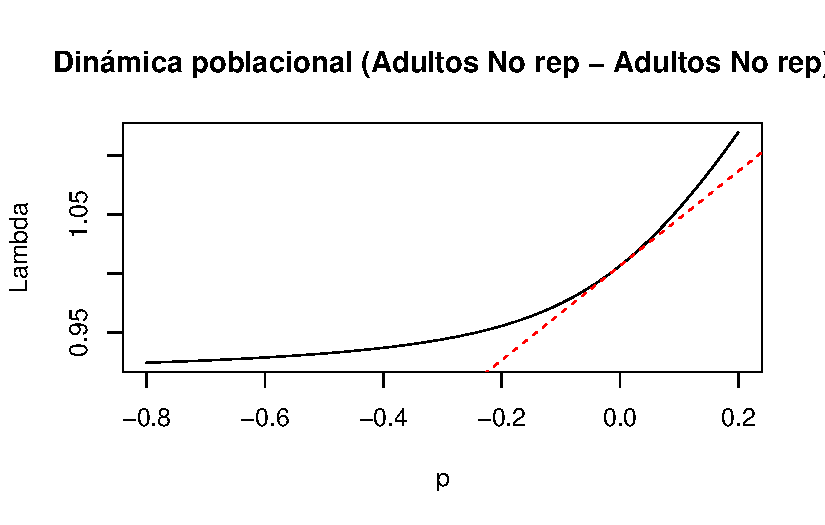
\includegraphics[keepaspectratio]{113-Funciones_de_Transferencia_files/figure-pdf/unnamed-chunk-5-1.pdf}}

\begin{center}\rule{0.5\linewidth}{0.5pt}\end{center}

\subsection{\texorpdfstring{b) Elasticidad no lineal: efecto del
crecimiento de la fase juvenil a reproductiva {[}4,2{]} sobre
\(\lambda\)}{b) Elasticidad no lineal: efecto del crecimiento de la fase juvenil a reproductiva {[}4,2{]} sobre \textbackslash lambda}}\label{b-elasticidad-no-lineal-efecto-del-crecimiento-de-la-fase-juvenil-a-reproductiva-42-sobre-lambda}

En este y los siguientes ejemplos, el análisis se centra en la
estructura de perturbación y la magnitud de la perturbación, ya que son
los componentes que varían. La perturbación correspondiente al
crecimiento o tránsito de la fase juvenil a adulto reproductivo
{[}4,2{]} se define mediante los siguientes vectores y rango:

\begin{itemize}
\tightlist
\item
  \texttt{d} = c(0, 1, 0, 0)
\item
  \texttt{e} = c(0, 0, 0, 1)
\item
  \texttt{prange} = seq(0, 0.89, 0.01)
\end{itemize}

Los resultados indican que la perturbación en esta transición ejerce un
efecto no lineal sobre λ. Este efecto es positivo para el crecimiento
poblacional, especialmente en niveles altos de perturbación.

Cuando la perturbación es menor a 0.2, el comportamiento no difiere
significativamente del esperado bajo elasticidad lineal, donde las
perturbaciones son pequeñas. Por lo tanto, en este rango, el impacto
sobre λ es prácticamente nulo.

En cambio, a medida que la magnitud de la perturbación aumenta, el
efecto sobre la tasa de crecimiento se intensifica, reflejando la
naturaleza no lineal del sistema.

\begin{Shaded}
\begin{Highlighting}[]
\CommentTok{\#Entrada de la matriz a(4,2): juveniles a adultos}
\NormalTok{tf5 }\OtherTok{\textless{}{-}} \FunctionTok{tfa\_lambda}\NormalTok{(Lr1,  }\AttributeTok{d =} \FunctionTok{c}\NormalTok{(}\DecValTok{0}\NormalTok{,}\DecValTok{1}\NormalTok{,}\DecValTok{0}\NormalTok{,}\DecValTok{0}\NormalTok{), }\AttributeTok{e =} \FunctionTok{c}\NormalTok{(}\DecValTok{0}\NormalTok{,}\DecValTok{0}\NormalTok{,}\DecValTok{0}\NormalTok{,}\DecValTok{1}\NormalTok{), }\AttributeTok{prange =} \FunctionTok{seq}\NormalTok{(}\DecValTok{0}\NormalTok{,}\FloatTok{0.89}\NormalTok{,}\FloatTok{0.01}\NormalTok{))}

\CommentTok{\#Gráfica de la dinámica poblacional}
\FunctionTok{plot}\NormalTok{(tf5, }\AttributeTok{ann =} \ConstantTok{FALSE}\NormalTok{)}
\FunctionTok{title}\NormalTok{(}\AttributeTok{main =} \StringTok{"Dinámica poblacional (Juveniles {-} Adultos)"}\NormalTok{, }\AttributeTok{ylab =} \StringTok{"Lambda"}\NormalTok{, }\AttributeTok{xlab =} \StringTok{"p"}\NormalTok{)}

\CommentTok{\#Cálculo de lambda{-}max:}
\NormalTok{lambda5 }\OtherTok{\textless{}{-}} \FunctionTok{Re}\NormalTok{(}\FunctionTok{eigen}\NormalTok{(Lr1)}\SpecialCharTok{$}\NormalTok{values[}\DecValTok{1}\NormalTok{]) }

\CommentTok{\#Cálculo de la sensibilidad}
\NormalTok{sens5 }\OtherTok{\textless{}{-}} \FunctionTok{tfs\_lambda}\NormalTok{(Lr1, }\AttributeTok{d =} \FunctionTok{c}\NormalTok{(}\DecValTok{0}\NormalTok{, }\DecValTok{1}\NormalTok{, }\DecValTok{0}\NormalTok{, }\DecValTok{0}\NormalTok{), }
                         \AttributeTok{e =} \FunctionTok{c}\NormalTok{(}\DecValTok{0}\NormalTok{, }\DecValTok{0}\NormalTok{, }\DecValTok{0}\NormalTok{, }\DecValTok{1}\NormalTok{))}

\CommentTok{\#Agregar la línea, especificando el intercepto y la pendiente}
\FunctionTok{abline}\NormalTok{(lambda5, sens5, }\AttributeTok{lty =} \DecValTok{2}\NormalTok{, }\AttributeTok{col =} \StringTok{"red"}\NormalTok{)}
\end{Highlighting}
\end{Shaded}

\pandocbounded{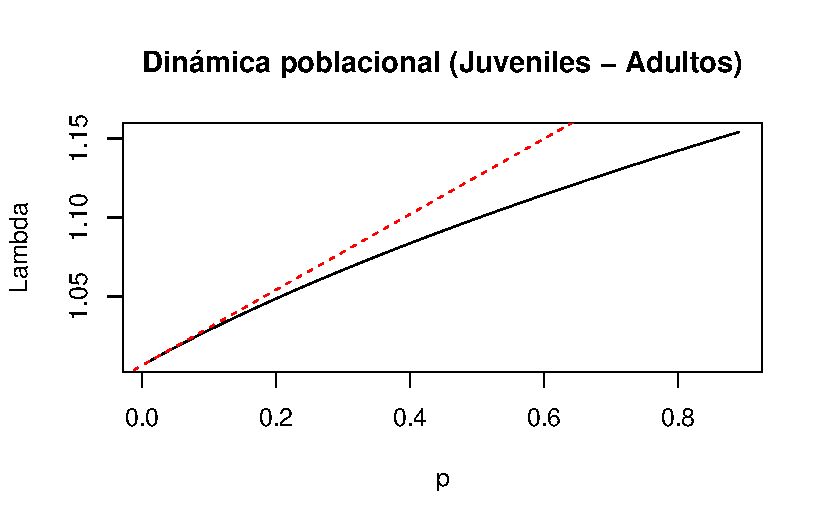
\includegraphics[keepaspectratio]{113-Funciones_de_Transferencia_files/figure-pdf/unnamed-chunk-6-1.pdf}}

\begin{center}\rule{0.5\linewidth}{0.5pt}\end{center}

\subsection{\texorpdfstring{c) Elasticidad no lineal: efecto del
retroceso del estado adulto reproductivo a no reproductivo {[}3,4{]}
sobre
\(\lambda\)}{c) Elasticidad no lineal: efecto del retroceso del estado adulto reproductivo a no reproductivo {[}3,4{]} sobre \textbackslash lambda}}\label{c-elasticidad-no-lineal-efecto-del-retroceso-del-estado-adulto-reproductivo-a-no-reproductivo-34-sobre-lambda}

En la perturbación correspondiente al retroceso o transición de la fase
adulta a adulto no reproductivo {[}3,4{]}, la ubicación vectorial se
define como:

\begin{itemize}
\tightlist
\item
  \texttt{d} = c(0, 0, 0, 1)
\item
  \texttt{e} = c(0, 0, 1, 0) y la magnitud de la perturbación se
  establece en:
\item
  \texttt{prange} = seq(0, 0.77, 0.01)
\end{itemize}

Los resultados indican que el efecto de esta perturbación sobre λ es no
lineal en niveles altos de perturbación, mientras que para
perturbaciones pequeñas (\textless{} 0.2) el comportamiento no difiere
significativamente del esperado bajo elasticidad lineal.

A medida que la magnitud de la perturbación aumenta, se observa un
efecto positivo sobre la tasa de crecimiento poblacional, lo que refleja
la importancia de esta transición en la dinámica transitoria.

\begin{Shaded}
\begin{Highlighting}[]
\CommentTok{\#Entrada de la matriz a(3,4): adultos reproductivos a NR}

\NormalTok{tf9 }\OtherTok{\textless{}{-}} \FunctionTok{tfa\_lambda}\NormalTok{(Lr1,  }\AttributeTok{d =} \FunctionTok{c}\NormalTok{(}\DecValTok{0}\NormalTok{, }\DecValTok{0}\NormalTok{, }\DecValTok{0}\NormalTok{, }\DecValTok{1}\NormalTok{),}
                       \AttributeTok{e =} \FunctionTok{c}\NormalTok{(}\DecValTok{0}\NormalTok{, }\DecValTok{0}\NormalTok{, }\DecValTok{1}\NormalTok{, }\DecValTok{0}\NormalTok{),}
                  \AttributeTok{prange =} \FunctionTok{seq}\NormalTok{(}\SpecialCharTok{{-}}\FloatTok{0.2}\NormalTok{, }\FloatTok{0.77}\NormalTok{, }\FloatTok{0.01}\NormalTok{))}

\CommentTok{\#Gráfica de la dinámica poblacional}
\FunctionTok{plot}\NormalTok{(tf9, }\AttributeTok{ann =} \ConstantTok{FALSE}\NormalTok{)}
\FunctionTok{title}\NormalTok{(}\AttributeTok{main =} \StringTok{"Dinámica poblacional (Adultos reproductivos {-} NR)"}\NormalTok{, }\AttributeTok{ylab =} \StringTok{"Lambda"}\NormalTok{, }\AttributeTok{xlab =} \StringTok{"p"}\NormalTok{)}

\CommentTok{\#Cálculo de lambda{-}max:}
\NormalTok{lambda9 }\OtherTok{\textless{}{-}} \FunctionTok{Re}\NormalTok{(}\FunctionTok{eigen}\NormalTok{(Lr1)}\SpecialCharTok{$}\NormalTok{values[}\DecValTok{1}\NormalTok{]) }

\CommentTok{\#Cálculo de la sensibilidad}
\NormalTok{sens9 }\OtherTok{\textless{}{-}} \FunctionTok{tfs\_lambda}\NormalTok{(Lr1, }\AttributeTok{d =} \FunctionTok{c}\NormalTok{(}\DecValTok{0}\NormalTok{, }\DecValTok{0}\NormalTok{, }\DecValTok{0}\NormalTok{, }\DecValTok{1}\NormalTok{), }
                        \AttributeTok{e =} \FunctionTok{c}\NormalTok{(}\DecValTok{0}\NormalTok{, }\DecValTok{0}\NormalTok{, }\DecValTok{1}\NormalTok{,  }\DecValTok{0}\NormalTok{))}

\CommentTok{\#Agregar la línea, especificando el intercepto y la pendiente}
\FunctionTok{abline}\NormalTok{(lambda9, sens9, }\AttributeTok{lty =} \DecValTok{2}\NormalTok{, }\AttributeTok{col =} \StringTok{"red"}\NormalTok{)}
\end{Highlighting}
\end{Shaded}

\pandocbounded{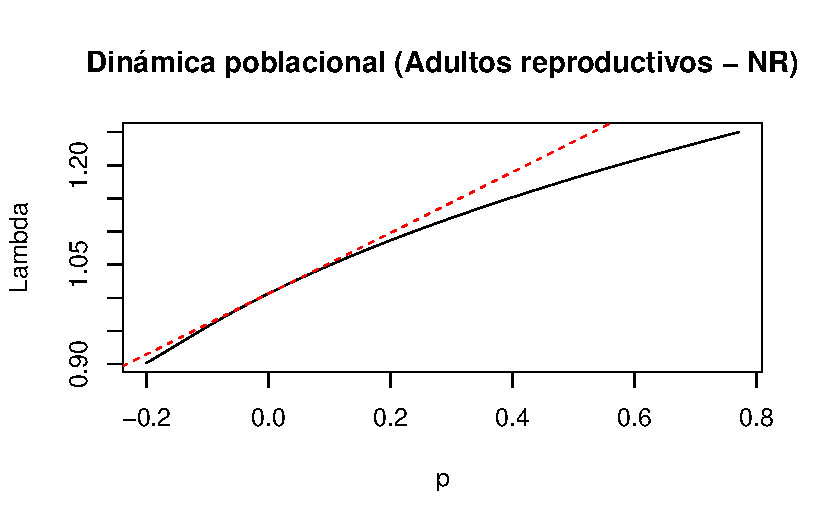
\includegraphics[keepaspectratio]{113-Funciones_de_Transferencia_files/figure-pdf/unnamed-chunk-7-1.pdf}}

\begin{center}\rule{0.5\linewidth}{0.5pt}\end{center}

\subsection{\texorpdfstring{d) Elasticidad no lineal: efecto de la
contribución reproductiva del estado adulto a plántula {[}1,4{]} sobre
\(\lambda\)}{d) Elasticidad no lineal: efecto de la contribución reproductiva del estado adulto a plántula {[}1,4{]} sobre \textbackslash lambda}}\label{d-elasticidad-no-lineal-efecto-de-la-contribuciuxf3n-reproductiva-del-estado-adulto-a-pluxe1ntula-14-sobre-lambda}

En la perturbación correspondiente a la contribución reproductiva de
adultos hacia plántulas ({[}1,4{]}), la ubicación vectorial se define
como:

\begin{itemize}
\tightlist
\item
  \texttt{d} = c(0, 0, 0, 1)
\item
  \texttt{e} = c(1, 0, 0, 0) y la magnitud de la perturbación se
  establece en:
\item
  \texttt{prange} = seq(-0.150, 0.85, 0.01)
\end{itemize}

Los resultados indican que la perturbación en esta transición produce un
efecto lineal sobre λ. Sin embargo, la pendiente asociada a la
elasticidad no lineal es menor en comparación con la sensibilidad
lineal, lo que sugiere que el impacto de esta transición sobre la tasa
de crecimiento poblacional es más limitado de lo que se esperaría bajo
un modelo estrictamente lineal.

\begin{Shaded}
\begin{Highlighting}[]
\CommentTok{\#Entrada de la matriz a(1,4): adultos reproductivos a plántulas}

\NormalTok{tf8 }\OtherTok{\textless{}{-}} \FunctionTok{tfa\_lambda}\NormalTok{(Lr1,  }\AttributeTok{d =} \FunctionTok{c}\NormalTok{(}\DecValTok{0}\NormalTok{,}\DecValTok{0}\NormalTok{,}\DecValTok{0}\NormalTok{,}\DecValTok{1}\NormalTok{),}
                       \AttributeTok{e =} \FunctionTok{c}\NormalTok{(}\DecValTok{1}\NormalTok{,}\DecValTok{0}\NormalTok{,}\DecValTok{0}\NormalTok{,}\DecValTok{0}\NormalTok{),}
                  \AttributeTok{prange =} \FunctionTok{seq}\NormalTok{(}\SpecialCharTok{{-}}\FloatTok{0.15}\NormalTok{,}\FloatTok{0.85}\NormalTok{,}\FloatTok{0.01}\NormalTok{))}

\CommentTok{\#Gráfica de la dinámica poblacional}
\FunctionTok{plot}\NormalTok{(tf8, }\AttributeTok{ann =} \ConstantTok{FALSE}\NormalTok{)}
\FunctionTok{title}\NormalTok{(}\AttributeTok{main =} \StringTok{"Dinámica poblacional (Adultos reproductivos {-} Plántulas)"}\NormalTok{, }\AttributeTok{ylab =} \StringTok{"Lambda"}\NormalTok{, }\AttributeTok{xlab =} \StringTok{"p"}\NormalTok{)}

\CommentTok{\#Cálculo de lambda{-}max:}
\NormalTok{lambda8 }\OtherTok{\textless{}{-}} \FunctionTok{Re}\NormalTok{(}\FunctionTok{eigen}\NormalTok{(Lr1)}\SpecialCharTok{$}\NormalTok{values[}\DecValTok{1}\NormalTok{]) }

\CommentTok{\#Cálculo de la sensibilidad}
\NormalTok{sens8 }\OtherTok{\textless{}{-}} \FunctionTok{tfs\_lambda}\NormalTok{(Lr1, }\AttributeTok{d =} \FunctionTok{c}\NormalTok{(}\DecValTok{1}\NormalTok{,}\DecValTok{0}\NormalTok{,}\DecValTok{0}\NormalTok{,}\DecValTok{0}\NormalTok{), }
                         \AttributeTok{e =} \FunctionTok{c}\NormalTok{(}\DecValTok{0}\NormalTok{,}\DecValTok{0}\NormalTok{,}\DecValTok{0}\NormalTok{,}\DecValTok{1}\NormalTok{))}

\CommentTok{\#Agregar la línea, especificando el intercepto y la pendiente}
\FunctionTok{abline}\NormalTok{(lambda8, sens8, }\AttributeTok{lty =} \DecValTok{2}\NormalTok{, }\AttributeTok{col =} \StringTok{"red"}\NormalTok{)}
\end{Highlighting}
\end{Shaded}

\pandocbounded{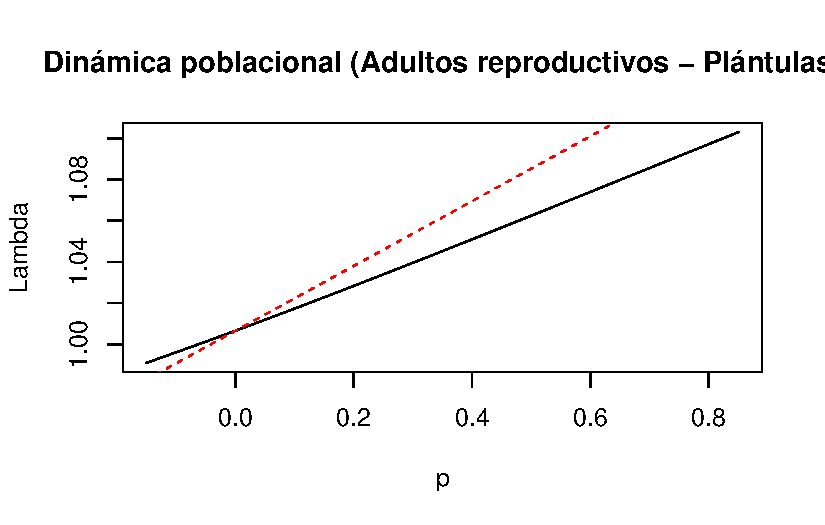
\includegraphics[keepaspectratio]{113-Funciones_de_Transferencia_files/figure-pdf/unnamed-chunk-8-1.pdf}}

\begin{center}\rule{0.5\linewidth}{0.5pt}\end{center}

\subsection{Elasticidad no lineal: uso de toda la matriz de proyección
poblacional}\label{elasticidad-no-lineal-uso-de-toda-la-matriz-de-proyecciuxf3n-poblacional}

La función \texttt{tfam\_lambda} permite estimar automáticamente la
elasticidad no lineal para todos los elementos distintos de cero en una
matriz poblacional, mientras que \texttt{tfmat\_lamb} genera las
gráficas correspondientes de manera automática. Stott y colaboradores
(Stott, Hodgson \& Townley, 2012b) recomiendan el uso de
\texttt{tfam\_lambda} debido a la dificultad que implica definir
manualmente la magnitud de la perturbación; por ello, este método
resulta más práctico. Sin embargo, es necesario considerar las
siguientes limitaciones:

\begin{itemize}
\tightlist
\item
  La asignación del tipo de elemento (por ejemplo, fecundidad o
  probabilidad de transición) en la matriz está predeterminada en el
  código de la función.
\item
  La magnitud de la perturbación también se calcula a partir de
  parámetros predefinidos en el código.
\end{itemize}

Estas condiciones pueden generar inconsistencias, ya que las
características de la especie analizada no siempre coinciden con los
criterios establecidos por el autor del código. Por ejemplo, en la
definición de elementos en la matriz \(A\), el código supone que todos
los valores del primer renglón corresponden a fecundidad (\(F\)). Sin
embargo, en el caso de \emph{L. rubripetala}, el elemento {[}1,1{]}
representa una probabilidad de transición (\(P\)), no una fecundidad.
Este problema se resuelve incorporando la función \texttt{elementtype},
que permite especificar el tipo de cada elemento.

Respecto a la magnitud de la perturbación, los valores predefinidos por
el autor (\texttt{Flim\ =\ (-1,\ 10)} y \texttt{Plim\ =\ (-1,\ 10)}) no
pueden modificarse. Esto implica que todos los elementos se perturban en
el mismo intervalo, lo cual es poco realista, ya que cada elemento
debería tener un rango específico según su naturaleza. En particular, el
límite superior de \texttt{Plim} puede generar valores mayores a 1, lo
que excede la probabilidad máxima permitida en una columna de la matriz
\(A\).

Por estas razones, para controlar mejor las variables del modelo y
adaptarlo a la especie de estudio, se recomienda utilizar la función
\texttt{tfa\_lambda} y agrupar las gráficas manualmente, de forma
similar a \texttt{tfmat\_lamb}. En la última sección del capítulo se
presenta el código correspondiente en \texttt{ggplot2}.

\begin{tcolorbox}[enhanced jigsaw, arc=.35mm, bottomrule=.15mm, bottomtitle=1mm, breakable, colback=white, colbacktitle=quarto-callout-warning-color!10!white, colframe=quarto-callout-warning-color-frame, coltitle=black, left=2mm, leftrule=.75mm, opacityback=0, opacitybacktitle=0.6, rightrule=.15mm, title=\textcolor{quarto-callout-warning-color}{\faExclamationTriangle}\hspace{0.5em}{Advertencia}, titlerule=0mm, toprule=.15mm, toptitle=1mm]

\textbf{Cuidado con los rangos \texttt{Plim} y \texttt{Flim}
predeterminados.} Las funciones \texttt{tfam\_lambda()} y
\texttt{tfam\_inertia()} usan rangos de perturbación fijos
(\texttt{Plim\ =\ c(-1,\ 10)} y \texttt{Flim\ =\ c(-1,\ 10)}) que
\textbf{no pueden modificarse}. Esto produce dos problemas:

\begin{itemize}
\tightlist
\item
  El límite superior (\texttt{+10}) puede generar valores de
  probabilidad mayores a 1, biológicamente imposibles.
\item
  El mismo rango se aplica a transiciones y a fecundidad, ignorando que
  cada elemento tiene un rango natural distinto.
\end{itemize}

Cuando los resultados parecen extremos o poco realistas, conviene usar
\texttt{tfa\_lambda()} por elemento con un \texttt{prange} específico
(basado en la biología de la especie) y agrupar las gráficas manualmente
con \texttt{cowplot::plot\_grid()}.

\end{tcolorbox}

\subsection{\texorpdfstring{Resultados del análisis con
\texttt{tfam\_lambda}}{Resultados del análisis con tfam\_lambda}}\label{resultados-del-anuxe1lisis-con-tfam_lambda}

En el ejemplo aplicado a \emph{L. rubripetala}, se obtuvieron los
siguientes resultados al ejecutar \texttt{tfam\_lambda} junto con la
función \texttt{elementtype}. Se generaron 10 gráficas, correspondientes
a los 10 elementos distintos de cero en la matriz \(A\). Cada gráfica se
ubica en la posición del elemento analizado. Los resultados muestran que
nueve de estas perturbaciones tienen un efecto no lineal sobre
\(\lambda\). En las gráficas, los valores del eje \emph{x} (intervalo de
perturbación, \(p\)) y del eje \emph{y} (\(\lambda\)) no comparten la
misma escala. Las gráficas incluyen únicamente la tendencia de la
elasticidad no lineal, aunque es posible añadir la línea de sensibilidad
asintótica mediante la función \texttt{abline}, como se hizo en los
ejemplos anteriores.

En cuanto a la interpretación, se observa que la permanencia en el mismo
estado de desarrollo no sigue un patrón lineal. Además, en cuatro
elementos, aumentar la perturbación por encima de ± 0.1 genera un efecto
positivo sobre \(\lambda\). El retroceso de juvenil a no reproductivo
muestra un efecto lineal y positivo sobre \(\lambda\). Aunque el efecto
no siempre es estrictamente lineal, el impacto positivo en el
crecimiento poblacional se mantiene en las transiciones: plántula a
juvenil, juvenil a adulto reproductivo, adulto no reproductivo a
reproductivo, y en la contribución reproductiva hacia plántulas.

\begin{Shaded}
\begin{Highlighting}[]
\NormalTok{n0 }\OtherTok{\textless{}{-}} \FunctionTok{c}\NormalTok{(}\DecValTok{0}\NormalTok{, }\DecValTok{46}\NormalTok{, }\DecValTok{38}\NormalTok{, }\DecValTok{82}\NormalTok{)}
\NormalTok{etype}\OtherTok{\textless{}{-}}\FunctionTok{matrix}\NormalTok{(}\FunctionTok{c}\NormalTok{(}\StringTok{"P"}\NormalTok{, }\StringTok{"F"}\NormalTok{, }\StringTok{"F"}\NormalTok{, }\StringTok{"F"}\NormalTok{, }
                \StringTok{"P"}\NormalTok{, }\StringTok{"P"}\NormalTok{, }\StringTok{"P"}\NormalTok{, }\StringTok{"P"}\NormalTok{, }
                \StringTok{"P"}\NormalTok{, }\StringTok{"P"}\NormalTok{, }\StringTok{"P"}\NormalTok{, }\StringTok{"P"}\NormalTok{, }
                \StringTok{"P"}\NormalTok{, }\StringTok{"P"}\NormalTok{, }\StringTok{"P"}\NormalTok{, }\StringTok{"P"}\NormalTok{), }\DecValTok{4}\NormalTok{,}\DecValTok{4}\NormalTok{)}

\NormalTok{tfmat\_lamb}\OtherTok{=}\FunctionTok{tfam\_lambda}\NormalTok{(Lr1, }\AttributeTok{elementtype =}\NormalTok{ etype)}

\FunctionTok{plot}\NormalTok{(tfmat\_lamb)}
\end{Highlighting}
\end{Shaded}

\pandocbounded{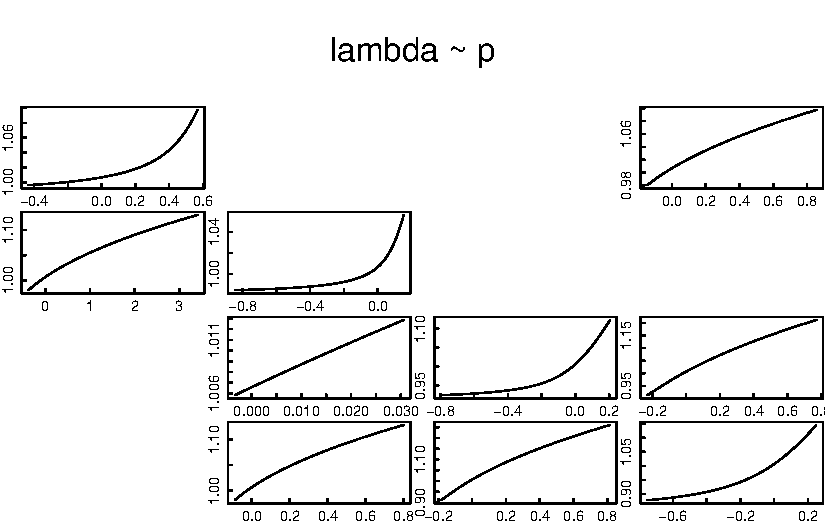
\includegraphics[keepaspectratio]{113-Funciones_de_Transferencia_files/figure-pdf/transF3-1.pdf}}

\begin{center}\rule{0.5\linewidth}{0.5pt}\end{center}

\section{Método de función de transferencia del efecto sobre la inercia
poblacional}\label{muxe9todo-de-funciuxf3n-de-transferencia-del-efecto-sobre-la-inercia-poblacional}

Tras una perturbación repentina en la estructura poblacional, pueden
producirse cambios en la densidad de individuos que modifican la forma
en que la población persiste a corto plazo, fenómeno conocido como
inercia poblacional. Esto ocurre porque, después de la perturbación, las
poblaciones presentan un comportamiento inestable que genera patrones de
crecimiento distintos a los esperados en una población equivalente con
distribución estable de estado o tamaño, en adelante denominada
población estable (Stott, Hodgson \& Townley, 2012a).

Como se explicó en el capítulo de \hyperref[Elasticidad]{Elasticidad},
una población estable crece de manera exponencial a una tasa constante
(\(\lambda\)) y mantiene una estructura proporcionalmente invariable.
Este patrón se altera cuando la población no está en equilibrio estable:
el crecimiento puede fluctuar y, a corto plazo, producir densidades
superiores o inferiores a las previstas bajo una distribución estable.
De igual forma, la estructura poblacional deja de mantenerse
proporcionalmente constante (Stott, Hodgson \& Townley, 2012a). La
función de transferencia permite calcular el efecto de la elasticidad no
lineal sobre la inercia poblacional a partir de la matriz de transición
de la especie y de los cambios en el vector de estructura poblacional.
Este cálculo se expresa como el cociente entre la densidad a corto plazo
de una población no estable y la densidad correspondiente a una
población estable. Su estimación se basa en una extensión de la segunda
ecuación del método de función de transferencia aplicado a \(\lambda\)
(Koons, Holmes \& Grand, 2007; Stott, Hodgson \& Townley, 2012a),
presentada previamente en este capítulo. La extensión se formula de la
siguiente manera:

\[
\mathbf{P}_\infty = \frac{\mathbf{v}^\top \hat{\mathbf{n}}_0 \, \|\mathbf{w}\|_1}{\mathbf{v}^\top \mathbf{w}}
\] Donde

\begin{itemize}
\item
  \(\mathbf{P}_\infty\)\\
  Representa la \textbf{población proyectada en el equilibrio
  asintótico} (cuando el sistema alcanza su estructura estable).
\item
  \(\mathbf{v}^\top\)\\
  Es el \textbf{vector propio izquierdo transpuesto} asociado al
  eigenvalor dominante de la matriz de proyección. Pondera los estados
  según su contribución al crecimiento.
\item
  \(\hat{\mathbf{n}}_0\)\\
  Es el \textbf{vector inicial de población normalizado}, que indica la
  distribución inicial entre clases o estados.
\item
  \(\mathbf{w}\)\\
  Es el \textbf{vector propio derecho}, que describe la
  \textbf{distribución estable por estados} cuando la población crece a
  la tasa asintótica.
\item
  \(\|\mathbf{w}\|_1\)\\
  Es la norma L₁ del vector (\(\mathbf{w}\)), equivalente a la suma de
  sus componentes. Se usa para escalar el vector estable.
\item
  \(\mathbf{v}^\top \mathbf{w}\)\\
  Es el \textbf{producto interno entre los eigenvectores izquierdo y
  derecho}, utilizado para normalizar la expresión.
\end{itemize}

Como resultado de la ecuación, se generan valores \textgreater1 y
\textless1 que corresponden al valor de la inercia poblacional a corto
plazo. La inercia \textgreater1 indica que la población crece y se
mantiene grande, mientras que los valores \textless1 indican que decrece
y se mantiene pequeña a corto plazo (Tremblay, Raventos \& Ackerman,
2015).

El efecto de una perturbación en la inercia poblacional a través del
método de función de transferencia se evalúa aplicando las funciones
\texttt{tfa\_inertia} o \texttt{tfam\_inertia} del paquete
\texttt{popdemo} de \textbf{R} (Stott, Hodgson \& Townley, 2012a). La
primera calcula la inercia poblacional al modificar un elemento de la
estructura poblacional, mientras que la segunda estima este parámetro al
modificar todos los elementos de la estructura poblacional de forma
automática.

\section{Cambios en la estructura poblacional y su efecto en la inercia
poblacional}\label{cambios-en-la-estructura-poblacional-y-su-efecto-en-la-inercia-poblacional}

Tremblay y colaboradores (Tremblay, Raventos \& Ackerman, 2015) usaron
las funciones \texttt{tfa\_inertia} y \texttt{tfam\_inertia} para
modelar la relación no lineal entre una perturbación ---o manipulación
en la estructura poblacional--- y la inercia del crecimiento poblacional
de \emph{L. rubripetala}. Dado que la persistencia de una población
puede evaluarse bajo distintos escenarios si se modifica un elemento de
la matriz de transición, estos autores evaluaron la inercia poblacional
considerando los siguientes supuestos:

\begin{enumerate}
\def\labelenumi{\alph{enumi})}
\tightlist
\item
  Un caso específico del ciclo de vida, por ejemplo el elemento con la
  elasticidad más alta.
\item
  Cambios en todos y cada uno de los elementos de la matriz \(A\).
\item
  Cambios en la última y la primera categoría de estado en la población.
\item
  Tomando en cuenta la estructura estable inicial, que evalúa la
  persistencia de la población si se encontrara en el equilibrio
  (Tremblay, Raventos \& Ackerman, 2015).
\end{enumerate}

Con base en estos escenarios, a continuación se describe cómo aplicar
\texttt{tfa\_inertia} y \texttt{tfam\_inertia}.

\subsection{\texorpdfstring{Elasticidad no lineal a través de
\texttt{tfa\_inertia}}{Elasticidad no lineal a través de tfa\_inertia}}\label{elasticidad-no-lineal-a-travuxe9s-de-tfa_inertia}

El primer escenario, un caso específico del ciclo de vida, permitirá
ejemplificar el uso de la función \texttt{tfa\_inertia}. En este se
evalúa el efecto de la estasis o permanencia en el estado no
reproductivo {[}3,3{]} sobre la inercia poblacional, y fue seleccionado
porque presenta el valor más alto de elasticidad. En el cálculo se usan
los siguientes argumentos para esta función: la matriz de transición de
la población \texttt{Lr1}, el vector de la estructura poblacional, la
estructura de perturbación (elemento de la matriz a perturbar) y la
magnitud de la perturbación
\texttt{prange\ =\ seq(-0.7954,\ 0.0205,\ 0.01)}. En el recuadro se
presenta el código correspondiente para su estimación.

Como resultado se genera una gráfica en la que se aprecia el
comportamiento de la inercia o persistencia poblacional a corto plazo
ante una perturbación. Esta respuesta se da de forma proporcional y
creciente, teniendo como puntos extremos en el eje \emph{x} la
perturbación mínima y la máxima. La línea roja representa la elasticidad
a perturbación cero, y la línea negra representa la función de
transferencia de la inercia poblacional ante cambios en la permanencia
en la fase de adulto no reproductivo.

La tendencia de la elasticidad no lineal sugiere que cualquier aumento
en la estasis en la categoría de adulto no reproductivo provocará una
disminución en el valor de la inercia poblacional a corto plazo.
Tremblay y colaboradores (Tremblay, Raventos \& Ackerman, 2015)
presentan en la figura 4 los resultados de los casos en que las
elasticidades fueron mayores.

\begin{Shaded}
\begin{Highlighting}[]
\NormalTok{n0 }\OtherTok{\textless{}{-}} \FunctionTok{c}\NormalTok{(}\DecValTok{0}\NormalTok{, }\DecValTok{46}\NormalTok{, }\DecValTok{38}\NormalTok{, }\DecValTok{82}\NormalTok{)}

\NormalTok{tf2}\OtherTok{\textless{}{-}}\FunctionTok{tfa\_inertia}\NormalTok{(Lr1, }\AttributeTok{vector=}\NormalTok{n0, }\AttributeTok{d=}\FunctionTok{c}\NormalTok{(}\DecValTok{0}\NormalTok{,}\DecValTok{0}\NormalTok{,}\DecValTok{1}\NormalTok{,}\DecValTok{0}\NormalTok{), }\AttributeTok{e=}\FunctionTok{c}\NormalTok{(}\DecValTok{0}\NormalTok{,}\DecValTok{0}\NormalTok{,}\DecValTok{1}\NormalTok{,}\DecValTok{0}\NormalTok{), }\AttributeTok{prange=}\FunctionTok{seq}\NormalTok{(}\SpecialCharTok{{-}}\FloatTok{0.8}\NormalTok{,}\FloatTok{0.2}\NormalTok{,}\FloatTok{0.01}\NormalTok{)) }\CommentTok{\# el efecto de perturbación de la transición de no reproductivo a adulto reproductivo}

\FunctionTok{plot}\NormalTok{(tf2, }\AttributeTok{main=}\StringTok{"Inercia poblacional"}\NormalTok{,}\AttributeTok{cex.axis=}\FloatTok{1.4}\NormalTok{,}\AttributeTok{cex.lab=}\FloatTok{1.5}\NormalTok{) }\CommentTok{\# gráfica de la inercia poblacional}

\NormalTok{inertia}\OtherTok{\textless{}{-}}\FunctionTok{inertia}\NormalTok{(Lr1, }\AttributeTok{vector=}\NormalTok{n0)}

\NormalTok{sens2}\OtherTok{\textless{}{-}}\FunctionTok{tfs\_inertia}\NormalTok{(Lr1, }\AttributeTok{vector=}\NormalTok{n0, }\AttributeTok{d=}\FunctionTok{c}\NormalTok{(}\DecValTok{0}\NormalTok{,}\DecValTok{0}\NormalTok{,}\DecValTok{1}\NormalTok{,}\DecValTok{0}\NormalTok{), }\AttributeTok{e=}\FunctionTok{c}\NormalTok{(}\DecValTok{0}\NormalTok{,}\DecValTok{0}\NormalTok{,}\DecValTok{1}\NormalTok{,}\DecValTok{0}\NormalTok{), }\AttributeTok{tolerance=}\FloatTok{1e{-}5}\NormalTok{) }\CommentTok{\# el efecto de sensibilidad de la inercia poblacional}
\FunctionTok{abline}\NormalTok{(inertia, sens2, }\AttributeTok{lty=}\DecValTok{2}\NormalTok{, }\AttributeTok{col=}\StringTok{"red"}\NormalTok{) }\CommentTok{\# Para añadir el efecto lineal }
\end{Highlighting}
\end{Shaded}

\pandocbounded{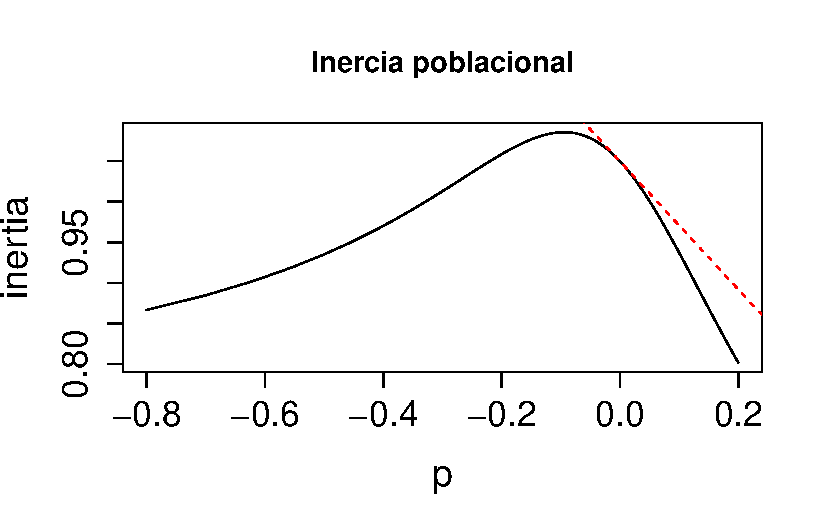
\includegraphics[keepaspectratio]{113-Funciones_de_Transferencia_files/figure-pdf/unnamed-chunk-9-1.pdf}}

\begin{center}\rule{0.5\linewidth}{0.5pt}\end{center}

\subsection{\texorpdfstring{Elasticidad no lineal a través de
\texttt{tfam\_inertia}}{Elasticidad no lineal a través de tfam\_inertia}}\label{elasticidad-no-lineal-a-travuxe9s-de-tfam_inertia}

En el cálculo de la inercia poblacional se puede optar por evaluar los
efectos de todas las entradas de la matriz con valor \textgreater0. La
función \texttt{tfam\_inertia} ofrece esta opción y su uso se
ejemplificará a través de los tres escenarios faltantes (b, c y d).

En este cálculo de la inercia poblacional se usan los siguientes
argumentos para esta función: la matriz de transición de la población
\texttt{Lr1}, el vector de la estructura poblacional, y, al igual que en
\texttt{tfam\_lambda}, se hacen los ajustes de los tipos de elementos en
la matriz con \texttt{elementtype}, y se mantienen los límites mínimo y
máximo de las funciones \texttt{Plim} y \texttt{Flim} definidos por el
autor del código.

A continuación se proyecta la persistencia de \emph{L. rubripetala} para
los tres escenarios faltantes: perturbación de todo el ciclo de vida,
concentración de individuos en la última y primera categoría, y la
estructura estable inicial.

\begin{itemize}
\tightlist
\item
  \emph{Perturbación de todo el ciclo de vida}. Los resultados de la
  simulación de perturbación de todos y cada uno de los elementos de la
  matriz (reproducción, crecimiento y supervivencia) sugieren que la
  permanencia en las cuatro fases del ciclo de vida de \emph{L.
  rubripetala} tiene un impacto negativo en la inercia poblacional.
  Cualquier aumento en la estasis o permanencia en alguno de los cuatro
  estados provocará una disminución en la densidad de la población a
  corto plazo.
\end{itemize}

A excepción del tránsito de adulto no reproductivo a reproductivo, el
tránsito a un estado superior tiene un efecto positivo en la inercia
poblacional. Lo mismo sucede con la retrogresión de adultos
reproductivos a no reproductivos y con la contribución reproductiva de
adultos a plántulas.

\begin{Shaded}
\begin{Highlighting}[]
\CommentTok{\#Definir márgenes}
\FunctionTok{par}\NormalTok{(}\AttributeTok{mfrow =} \FunctionTok{c}\NormalTok{(}\DecValTok{4}\NormalTok{,}\DecValTok{4}\NormalTok{))}
\FunctionTok{par}\NormalTok{(}\AttributeTok{mfg =} \FunctionTok{c}\NormalTok{(}\DecValTok{1}\NormalTok{,}\DecValTok{1}\NormalTok{))}

\CommentTok{\#Gráficas de la función de transferencia de la inercia en el ciclo de vida de L. rubripetala (población 1)}

\NormalTok{etype}\OtherTok{\textless{}{-}}\FunctionTok{matrix}\NormalTok{(}\FunctionTok{c}\NormalTok{(}\StringTok{"P"}\NormalTok{, }\StringTok{"F"}\NormalTok{, }\StringTok{"F"}\NormalTok{, }\StringTok{"F"}\NormalTok{, }
                \StringTok{"P"}\NormalTok{, }\StringTok{"P"}\NormalTok{, }\StringTok{"P"}\NormalTok{, }\StringTok{"P"}\NormalTok{, }
                \StringTok{"P"}\NormalTok{, }\StringTok{"P"}\NormalTok{, }\StringTok{"P"}\NormalTok{, }\StringTok{"P"}\NormalTok{, }
                \StringTok{"P"}\NormalTok{, }\StringTok{"P"}\NormalTok{, }\StringTok{"P"}\NormalTok{, }\StringTok{"P"}\NormalTok{), }\DecValTok{4}\NormalTok{,}\DecValTok{4}\NormalTok{)}

\NormalTok{tfmatriz }\OtherTok{\textless{}{-}} \FunctionTok{tfam\_inertia}\NormalTok{(Lr1, }\AttributeTok{elementtype =}\NormalTok{ etype, }\AttributeTok{vector =}\NormalTok{ nLr0)}

\FunctionTok{plot}\NormalTok{(tfmatriz,  }\AttributeTok{xlab=}\StringTok{"p"}\NormalTok{, }\AttributeTok{ylab=}\StringTok{"Inercia"}\NormalTok{, }\AttributeTok{cex.axis=}\FloatTok{1.4}\NormalTok{, }\AttributeTok{cex.lab=}\FloatTok{1.5}\NormalTok{)}
\end{Highlighting}
\end{Shaded}

\pandocbounded{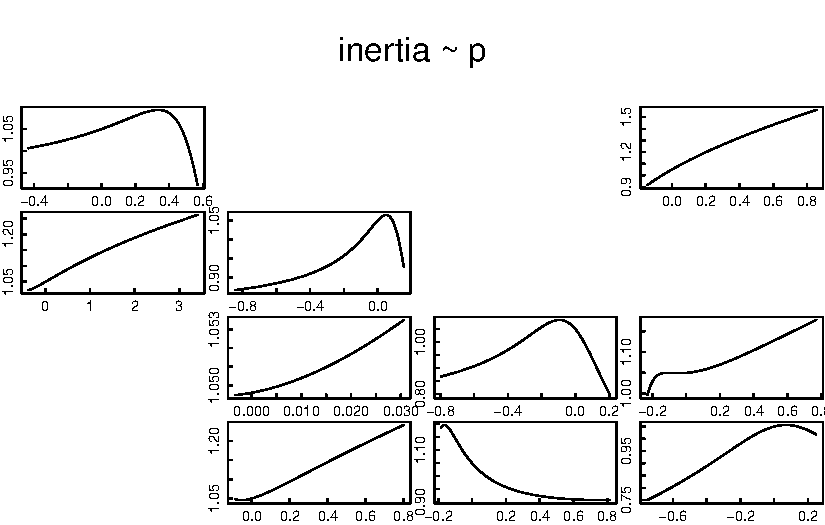
\includegraphics[keepaspectratio]{113-Funciones_de_Transferencia_files/figure-pdf/unnamed-chunk-10-1.pdf}}

\begin{center}\rule{0.5\linewidth}{0.5pt}\end{center}

\begin{itemize}
\item
  \emph{Última y primera categoría}. La función de transferencia de la
  inercia fue estimada al suponer que la población se encuentra
  concentrada en:

  \emph{i) la categoría de adulto reproductivo (Upper bound)}.
\end{itemize}

El código para el cálculo de la inercia poblacional se presenta en el
siguiente recuadro. En este se supone que la población está representada
por el último estado del ciclo de vida. Los resultados de la gráfica
(extremo inferior derecho) sugieren que cuando todos los individuos de
\emph{L. rubripetala} se encuentran en la fase de adulto reproductivo,
la inercia poblacional a corto plazo será mayor a 1.4, lo que indica que
la población puede crecer más del 40\% antes de alcanzar la tasa
constante de crecimiento poblacional. Asimismo, estos resultados indican
que los adultos reproductivos tienen un alto impacto positivo sobre la
tasa de crecimiento poblacional, a excepción de la transición de
juveniles a adultos no reproductivos.

\begin{Shaded}
\begin{Highlighting}[]
\NormalTok{etype}\OtherTok{\textless{}{-}}\FunctionTok{matrix}\NormalTok{(}\FunctionTok{c}\NormalTok{(}\StringTok{"P"}\NormalTok{, }\StringTok{"F"}\NormalTok{, }\StringTok{"F"}\NormalTok{, }\StringTok{"F"}\NormalTok{,}
                \StringTok{"P"}\NormalTok{, }\StringTok{"P"}\NormalTok{, }\StringTok{"P"}\NormalTok{, }\StringTok{"P"}\NormalTok{,}
                \StringTok{"P"}\NormalTok{, }\StringTok{"P"}\NormalTok{, }\StringTok{"P"}\NormalTok{, }\StringTok{"P"}\NormalTok{, }
                \StringTok{"P"}\NormalTok{, }\StringTok{"P"}\NormalTok{, }\StringTok{"P"}\NormalTok{, }\StringTok{"P"}\NormalTok{), }\DecValTok{4}\NormalTok{,}\DecValTok{4}\NormalTok{)}

\NormalTok{tfmatU}\OtherTok{=}\FunctionTok{tfam\_inertia}\NormalTok{(Lr1, }\AttributeTok{elementtype =}\NormalTok{ etype, }\AttributeTok{bound =} \StringTok{"upper"}\NormalTok{) }\CommentTok{\# donde todos los individuos están en el ultimo estadio}

\FunctionTok{plot}\NormalTok{(tfmatU, }\AttributeTok{cex.axis=}\FloatTok{1.4}\NormalTok{, }\AttributeTok{cex.lab=}\FloatTok{1.5}\NormalTok{) }\CommentTok{\# gráfica de la inercia poblacional}
\end{Highlighting}
\end{Shaded}

\pandocbounded{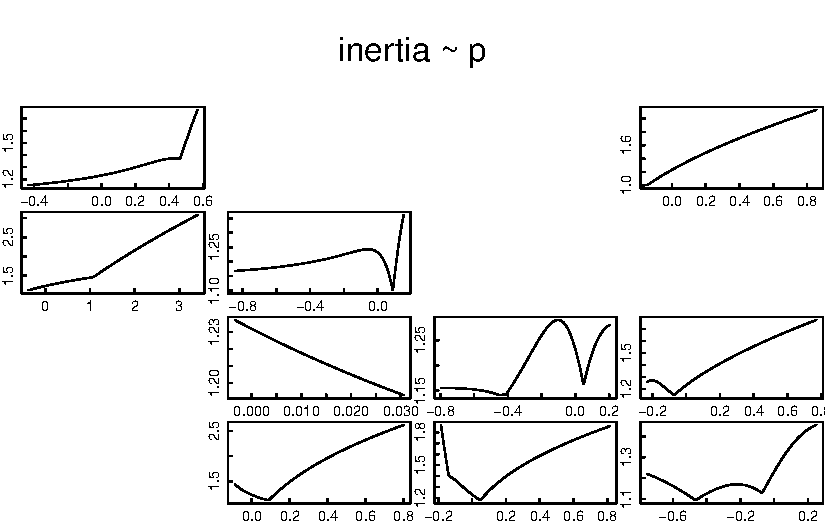
\includegraphics[keepaspectratio]{113-Funciones_de_Transferencia_files/figure-pdf/unnamed-chunk-11-1.pdf}}

\begin{center}\rule{0.5\linewidth}{0.5pt}\end{center}

\emph{ii) la categoría de plántulas (Lower bound)}.

El código del cálculo de la inercia poblacional al suponer que la
población está dominada por el primer estado del ciclo de vida se
presenta en el siguiente recuadro. Los resultados de la primera gráfica
(extremo superior derecho) sugieren que, al suponer que todos los
individuos de \emph{L. rubripetala} se concentran en el límite inferior,
la inercia poblacional a corto plazo es de 0.7, lo que indica que la
población puede reducirse hasta un 30\% antes de alcanzar la tasa
constante de crecimiento poblacional. En este escenario se reconoce que
la dominancia de las plántulas en la población tiene un impacto negativo
en el crecimiento de la población a corto plazo, ya que en todos los
casos la \(\lambda\) poblacional está por debajo de 1.

\begin{Shaded}
\begin{Highlighting}[]
\NormalTok{tfmatL}\OtherTok{=}\FunctionTok{tfam\_inertia}\NormalTok{(Lr1, }\AttributeTok{elementtype =}\NormalTok{ etype, }\AttributeTok{bound =} \StringTok{"lower"}\NormalTok{) }\CommentTok{\# donde todos los individuos están en el primer estadio}

\FunctionTok{plot}\NormalTok{(tfmatL)}
\end{Highlighting}
\end{Shaded}

\pandocbounded{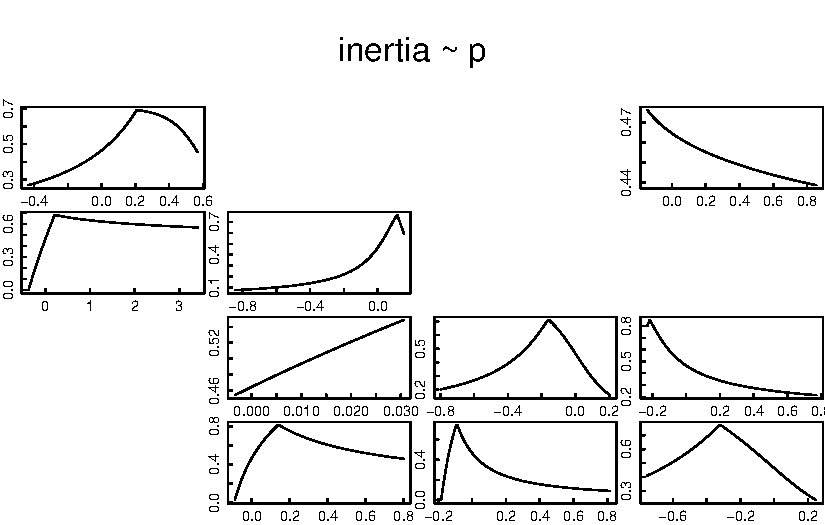
\includegraphics[keepaspectratio]{113-Funciones_de_Transferencia_files/figure-pdf/unnamed-chunk-12-1.pdf}}

\begin{center}\rule{0.5\linewidth}{0.5pt}\end{center}

\emph{iii) la estructura estable inicial}.

En el siguiente recuadro se presenta el código del cálculo de la inercia
poblacional para una población que se encuentra en su estructura estable
y, por tanto, en equilibrio. Los resultados de la primera gráfica
(extremo superior derecho) sugieren que la fecundidad tiene el mayor
impacto positivo en la dinámica transitoria si la población se encuentra
en equilibrio. En estas condiciones, duplicar la fecundidad aumenta
significativamente el tamaño de la población a corto plazo.

\begin{Shaded}
\begin{Highlighting}[]
\NormalTok{n0 }\OtherTok{\textless{}{-}} \FunctionTok{c}\NormalTok{(}\DecValTok{0}\NormalTok{, }\DecValTok{46}\NormalTok{, }\DecValTok{38}\NormalTok{, }\DecValTok{82}\NormalTok{)}

\NormalTok{stable }\OtherTok{\textless{}{-}}\NormalTok{ popbio}\SpecialCharTok{::}\FunctionTok{stable.stage}\NormalTok{(Lr1) }\CommentTok{\# calcular el estado estable de la matriz Lr1}

\NormalTok{tfmat\_I}\OtherTok{=}\FunctionTok{tfam\_inertia}\NormalTok{(Lr1, }\AttributeTok{elementtype =}\NormalTok{ etype, }\AttributeTok{vector =}\NormalTok{ stable) }\CommentTok{\# donde los individuos están en la estructura de población inicial}

\FunctionTok{plot}\NormalTok{(tfmat\_I)}
\end{Highlighting}
\end{Shaded}

\pandocbounded{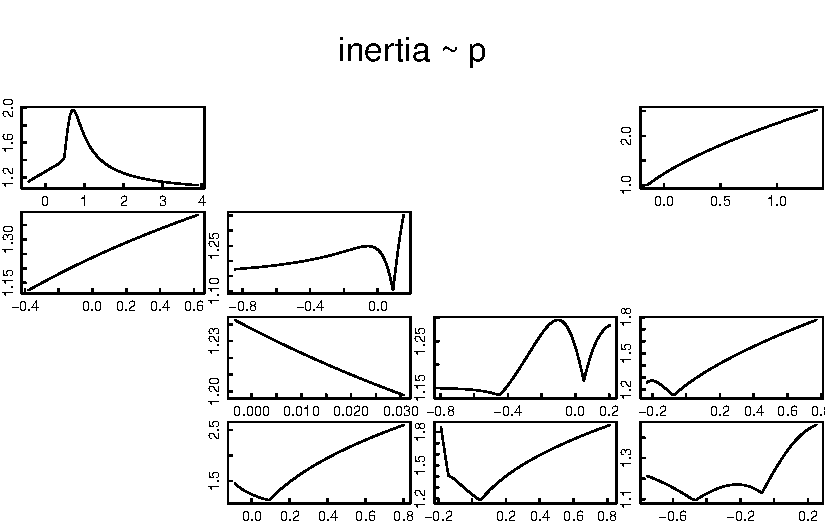
\includegraphics[keepaspectratio]{113-Funciones_de_Transferencia_files/figure-pdf/transF5-1.pdf}}

\begin{center}\rule{0.5\linewidth}{0.5pt}\end{center}

\section{Contenido extra}\label{contenido-extra}

\subsection{Uso de ggplot2 para la matriz de figuras generadas con la
función de
transferencia}\label{uso-de-ggplot2-para-la-matriz-de-figuras-generadas-con-la-funciuxf3n-de-transferencia}

En esta sección se presenta el código con \texttt{ggplot2} para agrupar
en una sola gráfica las 10 figuras generadas una por una para la matriz
\(A\) (ver §``Cambios en la estructura de perturbación y su efecto en la
tasa de crecimiento poblacional'') y las cuales ilustran el efecto de la
perturbación de cada elemento distinto de 0 sobre la inercia
poblacional. Esta sección resulta de gran utilidad y es una alternativa
muy buena al uso de \texttt{tfam\_lambda()} y \texttt{tfam\_inertia()},
ya que se evitarán los valores predeterminados en el código original
para \texttt{Flim} y \texttt{Plim}, permitiendo la descripción del
comportamiento de la especie con mayor certeza y basada en sus
parámetros poblacionales propios.

Finalmente, cabe señalar que con los ajustes necesarios, este código
puede ser aplicado a los resultados elemento por elemento de
\textbf{tfa\_inertia}.

\begin{Shaded}
\begin{Highlighting}[]
\NormalTok{tf1df}\OtherTok{=}\FunctionTok{as.data.frame}\NormalTok{(tf1)}
\NormalTok{tf1tf}\OtherTok{=}\NormalTok{ggplot2}\SpecialCharTok{::}\FunctionTok{ggplot}\NormalTok{() }\SpecialCharTok{+}
\NormalTok{  ggplot2}\SpecialCharTok{::}\FunctionTok{geom\_line}\NormalTok{(}\AttributeTok{data =}\NormalTok{ tf1df, }\FunctionTok{aes}\NormalTok{(}\AttributeTok{x =}\NormalTok{ p, }\AttributeTok{y =}\NormalTok{ lambda), }\AttributeTok{color =} \StringTok{"blue"}\NormalTok{) }\SpecialCharTok{+}
\NormalTok{  ggplot2}\SpecialCharTok{::}\FunctionTok{geom\_abline}\NormalTok{(}\AttributeTok{slope =}\NormalTok{ sens1, }\AttributeTok{intercept =}\NormalTok{ lambda1, }\AttributeTok{linetype =} \StringTok{"dashed"}\NormalTok{, }\AttributeTok{color =} \StringTok{"red"}\NormalTok{) }\SpecialCharTok{+}
  \CommentTok{\#ggplot2::labs(title = "P {-} P", x = "p", y = "Lambda") +}
\NormalTok{  ggplot2}\SpecialCharTok{::}\FunctionTok{theme\_minimal}\NormalTok{()}\SpecialCharTok{+}
  \FunctionTok{ylab}\NormalTok{(}\StringTok{""}\NormalTok{)}\SpecialCharTok{+}\FunctionTok{xlab}\NormalTok{(}\StringTok{""}\NormalTok{)}\SpecialCharTok{+}
  \FunctionTok{theme}\NormalTok{(}\AttributeTok{axis.text.x =} \FunctionTok{element\_text}\NormalTok{(}\AttributeTok{angle =} \DecValTok{45}\NormalTok{, }\AttributeTok{size=}\DecValTok{6}\NormalTok{),}
        \AttributeTok{axis.text.y =} \FunctionTok{element\_text}\NormalTok{(}\AttributeTok{size=}\DecValTok{6}\NormalTok{))}
  

\NormalTok{tf2df}\OtherTok{=}\FunctionTok{as.data.frame}\NormalTok{(tf2)}
\NormalTok{tf2tf}\OtherTok{=}\NormalTok{ggplot2}\SpecialCharTok{::}\FunctionTok{ggplot}\NormalTok{() }\SpecialCharTok{+}
\NormalTok{  ggplot2}\SpecialCharTok{::}\FunctionTok{geom\_line}\NormalTok{(}\AttributeTok{data =}\NormalTok{ tf2df, }\FunctionTok{aes}\NormalTok{(}\AttributeTok{x =}\NormalTok{ p, }\AttributeTok{y =}\NormalTok{ lambda), }\AttributeTok{color =} \StringTok{"blue"}\NormalTok{) }\SpecialCharTok{+}
\NormalTok{  ggplot2}\SpecialCharTok{::}\FunctionTok{geom\_abline}\NormalTok{(}\AttributeTok{slope =}\NormalTok{ sens2, }\AttributeTok{intercept =}\NormalTok{ lambda2, }\AttributeTok{linetype =} \StringTok{"dashed"}\NormalTok{, }\AttributeTok{color =} \StringTok{"red"}\NormalTok{) }\SpecialCharTok{+}
 \CommentTok{\# ggplot2::labs(title = "P {-} J", x = "p", y = "Lambda") +}
\NormalTok{  ggplot2}\SpecialCharTok{::}\FunctionTok{theme\_minimal}\NormalTok{()}\SpecialCharTok{+}
  \FunctionTok{ylab}\NormalTok{(}\StringTok{""}\NormalTok{)}\SpecialCharTok{+}\FunctionTok{xlab}\NormalTok{(}\StringTok{""}\NormalTok{)}\SpecialCharTok{+}
  \FunctionTok{theme}\NormalTok{(}\AttributeTok{axis.text.x =} \FunctionTok{element\_text}\NormalTok{(}\AttributeTok{angle =} \DecValTok{45}\NormalTok{, }\AttributeTok{size=}\DecValTok{6}\NormalTok{),}
        \AttributeTok{axis.text.y =} \FunctionTok{element\_text}\NormalTok{(}\AttributeTok{size=}\DecValTok{6}\NormalTok{))}

\NormalTok{tf3df}\OtherTok{=}\FunctionTok{as.data.frame}\NormalTok{(tf3)}
\NormalTok{tf3tf}\OtherTok{=}\NormalTok{ggplot2}\SpecialCharTok{::}\FunctionTok{ggplot}\NormalTok{() }\SpecialCharTok{+}
\NormalTok{  ggplot2}\SpecialCharTok{::}\FunctionTok{geom\_line}\NormalTok{(}\AttributeTok{data =}\NormalTok{ tf3df, }\FunctionTok{aes}\NormalTok{(}\AttributeTok{x =}\NormalTok{ p, }\AttributeTok{y =}\NormalTok{ lambda), }\AttributeTok{color =} \StringTok{"blue"}\NormalTok{) }\SpecialCharTok{+}
\NormalTok{  ggplot2}\SpecialCharTok{::}\FunctionTok{geom\_abline}\NormalTok{(}\AttributeTok{slope =}\NormalTok{ sens3, }\AttributeTok{intercept =}\NormalTok{ lambda3, }\AttributeTok{linetype =} \StringTok{"dashed"}\NormalTok{, }\AttributeTok{color =} \StringTok{"red"}\NormalTok{) }\SpecialCharTok{+}
  \CommentTok{\#ggplot2::labs(title = "J {-} J", x = "p", y = "Lambda") +}
\NormalTok{  ggplot2}\SpecialCharTok{::}\FunctionTok{theme\_minimal}\NormalTok{()}\SpecialCharTok{+}
  \FunctionTok{ylab}\NormalTok{(}\StringTok{""}\NormalTok{)}\SpecialCharTok{+}\FunctionTok{xlab}\NormalTok{(}\StringTok{""}\NormalTok{)}\SpecialCharTok{+}
  \FunctionTok{theme}\NormalTok{(}\AttributeTok{axis.text.x =} \FunctionTok{element\_text}\NormalTok{(}\AttributeTok{angle =} \DecValTok{45}\NormalTok{, }\AttributeTok{size=}\DecValTok{6}\NormalTok{),}
        \AttributeTok{axis.text.y =} \FunctionTok{element\_text}\NormalTok{(}\AttributeTok{size=}\DecValTok{6}\NormalTok{))}

\NormalTok{tf4df}\OtherTok{=}\FunctionTok{as.data.frame}\NormalTok{(tf4)}

\NormalTok{tf4tf}\OtherTok{=}\NormalTok{ggplot2}\SpecialCharTok{::}\FunctionTok{ggplot}\NormalTok{() }\SpecialCharTok{+}
\NormalTok{  ggplot2}\SpecialCharTok{::}\FunctionTok{geom\_line}\NormalTok{(}\AttributeTok{data =}\NormalTok{ tf4df, }\FunctionTok{aes}\NormalTok{(}\AttributeTok{x =}\NormalTok{ p, }\AttributeTok{y =}\NormalTok{ lambda), }\AttributeTok{color =} \StringTok{"blue"}\NormalTok{) }\SpecialCharTok{+}
\NormalTok{  ggplot2}\SpecialCharTok{::}\FunctionTok{geom\_abline}\NormalTok{(}\AttributeTok{slope =}\NormalTok{ sens4, }\AttributeTok{intercept =}\NormalTok{ lambda4, }\AttributeTok{linetype =} \StringTok{"dashed"}\NormalTok{, }\AttributeTok{color =} \StringTok{"red"}\NormalTok{) }\SpecialCharTok{+}
 \CommentTok{\# ggplot2::labs(title = "J {-} NR", x = "p", y = "Lambda") +}
\NormalTok{  ggplot2}\SpecialCharTok{::}\FunctionTok{theme\_minimal}\NormalTok{()}\SpecialCharTok{+}
  \FunctionTok{ylab}\NormalTok{(}\StringTok{""}\NormalTok{)}\SpecialCharTok{+}\FunctionTok{xlab}\NormalTok{(}\StringTok{""}\NormalTok{)}\SpecialCharTok{+}
  \FunctionTok{theme}\NormalTok{(}\AttributeTok{axis.text.x =} \FunctionTok{element\_text}\NormalTok{(}\AttributeTok{angle =} \DecValTok{45}\NormalTok{, }\AttributeTok{size=}\DecValTok{6}\NormalTok{),}
        \AttributeTok{axis.text.y =} \FunctionTok{element\_text}\NormalTok{(}\AttributeTok{size=}\DecValTok{6}\NormalTok{))}

\NormalTok{tf5df}\OtherTok{=}\FunctionTok{as.data.frame}\NormalTok{(tf5)}

\NormalTok{tf5tf}\OtherTok{=}\NormalTok{ggplot2}\SpecialCharTok{::}\FunctionTok{ggplot}\NormalTok{() }\SpecialCharTok{+}
\NormalTok{  ggplot2}\SpecialCharTok{::}\FunctionTok{geom\_line}\NormalTok{(}\AttributeTok{data =}\NormalTok{ tf5df, }\FunctionTok{aes}\NormalTok{(}\AttributeTok{x =}\NormalTok{ p, }\AttributeTok{y =}\NormalTok{ lambda), }\AttributeTok{color =} \StringTok{"blue"}\NormalTok{) }\SpecialCharTok{+}
\NormalTok{  ggplot2}\SpecialCharTok{::}\FunctionTok{geom\_abline}\NormalTok{(}\AttributeTok{slope =}\NormalTok{ sens5, }\AttributeTok{intercept =}\NormalTok{ lambda5, }\AttributeTok{linetype =} \StringTok{"dashed"}\NormalTok{, }\AttributeTok{color =} \StringTok{"red"}\NormalTok{) }\SpecialCharTok{+}
 \CommentTok{\# ggplot2::labs(title = "J {-} A", x = "p", y = "Lambda") +}
\NormalTok{  ggplot2}\SpecialCharTok{::}\FunctionTok{theme\_minimal}\NormalTok{()}\SpecialCharTok{+}
  \FunctionTok{ylab}\NormalTok{(}\StringTok{""}\NormalTok{)}\SpecialCharTok{+}\FunctionTok{xlab}\NormalTok{(}\StringTok{""}\NormalTok{)}\SpecialCharTok{+}
  \FunctionTok{theme}\NormalTok{(}\AttributeTok{axis.text.x =} \FunctionTok{element\_text}\NormalTok{(}\AttributeTok{angle =} \DecValTok{45}\NormalTok{, }\AttributeTok{size=}\DecValTok{6}\NormalTok{),}
        \AttributeTok{axis.text.y =} \FunctionTok{element\_text}\NormalTok{(}\AttributeTok{size=}\DecValTok{6}\NormalTok{))}

\NormalTok{tf6df}\OtherTok{=}\FunctionTok{as.data.frame}\NormalTok{(tf6)}

\NormalTok{tf6tf}\OtherTok{=}\NormalTok{ggplot2}\SpecialCharTok{::}\FunctionTok{ggplot}\NormalTok{() }\SpecialCharTok{+}
\NormalTok{  ggplot2}\SpecialCharTok{::}\FunctionTok{geom\_line}\NormalTok{(}\AttributeTok{data =}\NormalTok{ tf6df, }\FunctionTok{aes}\NormalTok{(}\AttributeTok{x =}\NormalTok{ p, }\AttributeTok{y =}\NormalTok{ lambda), }\AttributeTok{color =} \StringTok{"blue"}\NormalTok{) }\SpecialCharTok{+}
\NormalTok{  ggplot2}\SpecialCharTok{::}\FunctionTok{geom\_abline}\NormalTok{(}\AttributeTok{slope =}\NormalTok{ sens6, }\AttributeTok{intercept =}\NormalTok{ lambda6, }\AttributeTok{linetype =} \StringTok{"dashed"}\NormalTok{, }\AttributeTok{color =} \StringTok{"red"}\NormalTok{) }\SpecialCharTok{+}
  \CommentTok{\#ggplot2::labs(title = "NR {-} NR", x = "p", y = "Lambda") +}
\NormalTok{  ggplot2}\SpecialCharTok{::}\FunctionTok{theme\_minimal}\NormalTok{()}\SpecialCharTok{+}
  \FunctionTok{ylab}\NormalTok{(}\StringTok{""}\NormalTok{)}\SpecialCharTok{+}\FunctionTok{xlab}\NormalTok{(}\StringTok{""}\NormalTok{)}\SpecialCharTok{+}
  \FunctionTok{theme}\NormalTok{(}\AttributeTok{axis.text.x =} \FunctionTok{element\_text}\NormalTok{(}\AttributeTok{angle =} \DecValTok{45}\NormalTok{, }\AttributeTok{size=}\DecValTok{6}\NormalTok{),}
        \AttributeTok{axis.text.y =} \FunctionTok{element\_text}\NormalTok{(}\AttributeTok{size=}\DecValTok{6}\NormalTok{))}

\NormalTok{tf7df}\OtherTok{=}\FunctionTok{as.data.frame}\NormalTok{(tf7)}

\NormalTok{tf7tf}\OtherTok{=}\NormalTok{ggplot2}\SpecialCharTok{::}\FunctionTok{ggplot}\NormalTok{() }\SpecialCharTok{+}
\NormalTok{  ggplot2}\SpecialCharTok{::}\FunctionTok{geom\_line}\NormalTok{(}\AttributeTok{data =}\NormalTok{ tf7df, }\FunctionTok{aes}\NormalTok{(}\AttributeTok{x =}\NormalTok{ p, }\AttributeTok{y =}\NormalTok{ lambda), }\AttributeTok{color =} \StringTok{"blue"}\NormalTok{) }\SpecialCharTok{+}
\NormalTok{  ggplot2}\SpecialCharTok{::}\FunctionTok{geom\_abline}\NormalTok{(}\AttributeTok{slope =}\NormalTok{ sens7, }\AttributeTok{intercept =}\NormalTok{ lambda7, }\AttributeTok{linetype =} \StringTok{"dashed"}\NormalTok{, }\AttributeTok{color =} \StringTok{"red"}\NormalTok{) }\SpecialCharTok{+}
 \CommentTok{\# ggplot2::labs(title = "NR {-} A", x = "p", y = "Lambda") +}
\NormalTok{  ggplot2}\SpecialCharTok{::}\FunctionTok{theme\_minimal}\NormalTok{()}\SpecialCharTok{+}
  \FunctionTok{ylab}\NormalTok{(}\StringTok{""}\NormalTok{)}\SpecialCharTok{+}\FunctionTok{xlab}\NormalTok{(}\StringTok{""}\NormalTok{)}\SpecialCharTok{+}
  \FunctionTok{theme}\NormalTok{(}\AttributeTok{axis.text.x =} \FunctionTok{element\_text}\NormalTok{(}\AttributeTok{angle =} \DecValTok{45}\NormalTok{, }\AttributeTok{size=}\DecValTok{6}\NormalTok{),}
        \AttributeTok{axis.text.y =} \FunctionTok{element\_text}\NormalTok{(}\AttributeTok{size=}\DecValTok{6}\NormalTok{))}

\NormalTok{tf8df}\OtherTok{=}\FunctionTok{as.data.frame}\NormalTok{(tf8)}

\NormalTok{tf8tf}\OtherTok{=}\NormalTok{ggplot2}\SpecialCharTok{::}\FunctionTok{ggplot}\NormalTok{() }\SpecialCharTok{+}
\NormalTok{  ggplot2}\SpecialCharTok{::}\FunctionTok{geom\_line}\NormalTok{(}\AttributeTok{data =}\NormalTok{ tf8df, }\FunctionTok{aes}\NormalTok{(}\AttributeTok{x =}\NormalTok{ p, }\AttributeTok{y =}\NormalTok{ lambda), }\AttributeTok{color =} \StringTok{"blue"}\NormalTok{) }\SpecialCharTok{+}
\NormalTok{  ggplot2}\SpecialCharTok{::}\FunctionTok{geom\_abline}\NormalTok{(}\AttributeTok{slope =}\NormalTok{ sens8, }\AttributeTok{intercept =}\NormalTok{ lambda8, }\AttributeTok{linetype =} \StringTok{"dashed"}\NormalTok{, }\AttributeTok{color =} \StringTok{"red"}\NormalTok{) }\SpecialCharTok{+}
 \CommentTok{\# ggplot2::labs(title = "A {-} F", x = "p", y = "Lambda") +}
\NormalTok{  ggplot2}\SpecialCharTok{::}\FunctionTok{theme\_minimal}\NormalTok{()}\SpecialCharTok{+}
  \FunctionTok{ylab}\NormalTok{(}\StringTok{""}\NormalTok{)}\SpecialCharTok{+}\FunctionTok{xlab}\NormalTok{(}\StringTok{""}\NormalTok{)}\SpecialCharTok{+}
  \FunctionTok{theme}\NormalTok{(}\AttributeTok{axis.text.x =} \FunctionTok{element\_text}\NormalTok{(}\AttributeTok{angle =} \DecValTok{45}\NormalTok{, }\AttributeTok{size=}\DecValTok{6}\NormalTok{),}
        \AttributeTok{axis.text.y =} \FunctionTok{element\_text}\NormalTok{(}\AttributeTok{size=}\DecValTok{6}\NormalTok{))}

\NormalTok{tf9df}\OtherTok{=}\FunctionTok{as.data.frame}\NormalTok{(tf9)}

\NormalTok{tf9tf}\OtherTok{=}\NormalTok{ggplot2}\SpecialCharTok{::}\FunctionTok{ggplot}\NormalTok{() }\SpecialCharTok{+}
\NormalTok{  ggplot2}\SpecialCharTok{::}\FunctionTok{geom\_line}\NormalTok{(}\AttributeTok{data =}\NormalTok{ tf9df, }\FunctionTok{aes}\NormalTok{(}\AttributeTok{x =}\NormalTok{ p, }\AttributeTok{y =}\NormalTok{ lambda), }\AttributeTok{color =} \StringTok{"blue"}\NormalTok{) }\SpecialCharTok{+}
\NormalTok{  ggplot2}\SpecialCharTok{::}\FunctionTok{geom\_abline}\NormalTok{(}\AttributeTok{slope =}\NormalTok{ sens9, }\AttributeTok{intercept =}\NormalTok{ lambda9, }\AttributeTok{linetype =} \StringTok{"dashed"}\NormalTok{, }\AttributeTok{color =} \StringTok{"red"}\NormalTok{) }\SpecialCharTok{+}
 \CommentTok{\# ggplot2::labs(title = "A {-} NR", x = "p", y = "Lambda") +}
\NormalTok{  ggplot2}\SpecialCharTok{::}\FunctionTok{theme\_minimal}\NormalTok{()}\SpecialCharTok{+}
  \FunctionTok{ylab}\NormalTok{(}\StringTok{""}\NormalTok{)}\SpecialCharTok{+}\FunctionTok{xlab}\NormalTok{(}\StringTok{""}\NormalTok{)}\SpecialCharTok{+}
  \FunctionTok{theme}\NormalTok{(}\AttributeTok{axis.text.x =} \FunctionTok{element\_text}\NormalTok{(}\AttributeTok{angle =} \DecValTok{45}\NormalTok{, }\AttributeTok{size=}\DecValTok{6}\NormalTok{),}
        \AttributeTok{axis.text.y =} \FunctionTok{element\_text}\NormalTok{(}\AttributeTok{size=}\DecValTok{6}\NormalTok{))}

\NormalTok{tf10df}\OtherTok{=}\FunctionTok{as.data.frame}\NormalTok{(tf10)}
\NormalTok{tf10tf}\OtherTok{=}\NormalTok{ggplot2}\SpecialCharTok{::}\FunctionTok{ggplot}\NormalTok{() }\SpecialCharTok{+}
\NormalTok{  ggplot2}\SpecialCharTok{::}\FunctionTok{geom\_line}\NormalTok{(}\AttributeTok{data =}\NormalTok{ tf10df, }\FunctionTok{aes}\NormalTok{(}\AttributeTok{x =}\NormalTok{ p, }\AttributeTok{y =}\NormalTok{ lambda), }\AttributeTok{color =} \StringTok{"blue"}\NormalTok{) }\SpecialCharTok{+}
\NormalTok{  ggplot2}\SpecialCharTok{::}\FunctionTok{geom\_abline}\NormalTok{(}\AttributeTok{slope =}\NormalTok{ sens10, }\AttributeTok{intercept =}\NormalTok{ lambda10, }\AttributeTok{linetype =} \StringTok{"dashed"}\NormalTok{, }\AttributeTok{color =} \StringTok{"red"}\NormalTok{) }\SpecialCharTok{+}
  \CommentTok{\#ggplot2::labs(title = "A {-} A", x = "p", y = "Lambda") +}
\NormalTok{  ggplot2}\SpecialCharTok{::}\FunctionTok{theme\_minimal}\NormalTok{()}\SpecialCharTok{+}
  \FunctionTok{ylab}\NormalTok{(}\StringTok{""}\NormalTok{)}\SpecialCharTok{+}\FunctionTok{xlab}\NormalTok{(}\StringTok{""}\NormalTok{)}\SpecialCharTok{+}
  \FunctionTok{theme}\NormalTok{(}\AttributeTok{axis.text.x =} \FunctionTok{element\_text}\NormalTok{(}\AttributeTok{angle =} \DecValTok{45}\NormalTok{, }\AttributeTok{size=}\DecValTok{6}\NormalTok{),}
        \AttributeTok{axis.text.y =} \FunctionTok{element\_text}\NormalTok{(}\AttributeTok{size=}\DecValTok{6}\NormalTok{))}
\end{Highlighting}
\end{Shaded}

\begin{Shaded}
\begin{Highlighting}[]
\NormalTok{label }\OtherTok{\textless{}{-}} \FunctionTok{substitute}\NormalTok{(}
  \FunctionTok{paste}\NormalTok{(rho)}
\NormalTok{) }\CommentTok{\# este código es para poner el símbolo de "rho" en el eje "x" de la figura}

\NormalTok{cowplot}\SpecialCharTok{::}\FunctionTok{plot\_grid}\NormalTok{(tf1tf, }\ConstantTok{NULL}\NormalTok{, }\ConstantTok{NULL}\NormalTok{, tf8tf,   }\CommentTok{\# nota que los NULL son para dejar espacios vacíos}
\NormalTok{                   tf2tf, tf3tf, }\ConstantTok{NULL}\NormalTok{, }\ConstantTok{NULL}\NormalTok{,  }
                   \ConstantTok{NULL}\NormalTok{,  tf4tf, tf6tf, tf9tf,}
                   \ConstantTok{NULL}\NormalTok{,  tf5tf, tf7tf,  tf10tf, }
                   \AttributeTok{ncol =} \DecValTok{4}\NormalTok{, }\AttributeTok{nrow =} \DecValTok{4}\NormalTok{)}\SpecialCharTok{+}
\NormalTok{cowplot}\SpecialCharTok{::}\FunctionTok{draw\_label}\NormalTok{(}\StringTok{"Lambda"}\NormalTok{, }\AttributeTok{x =} \FloatTok{0.05}\NormalTok{, }\AttributeTok{y =} \FloatTok{0.5}\NormalTok{, }\AttributeTok{vjust =} \SpecialCharTok{{-}}\DecValTok{1}\NormalTok{, }\AttributeTok{size =} \DecValTok{14}\NormalTok{, }\AttributeTok{angle =} \DecValTok{90}\NormalTok{, }\AttributeTok{hjust =} \FloatTok{0.5}\NormalTok{)}\SpecialCharTok{+}
\NormalTok{cowplot}\SpecialCharTok{::}\FunctionTok{draw\_label}\NormalTok{(label, }\AttributeTok{x =} \FloatTok{0.5}\NormalTok{, }\AttributeTok{y =} \SpecialCharTok{{-}}\FloatTok{0.01}\NormalTok{, }\AttributeTok{vjust =} \SpecialCharTok{{-}}\DecValTok{1}\NormalTok{, }\AttributeTok{size =} \DecValTok{14}\NormalTok{, }\AttributeTok{hjust =} \FloatTok{0.5}\NormalTok{)}
\end{Highlighting}
\end{Shaded}

\pandocbounded{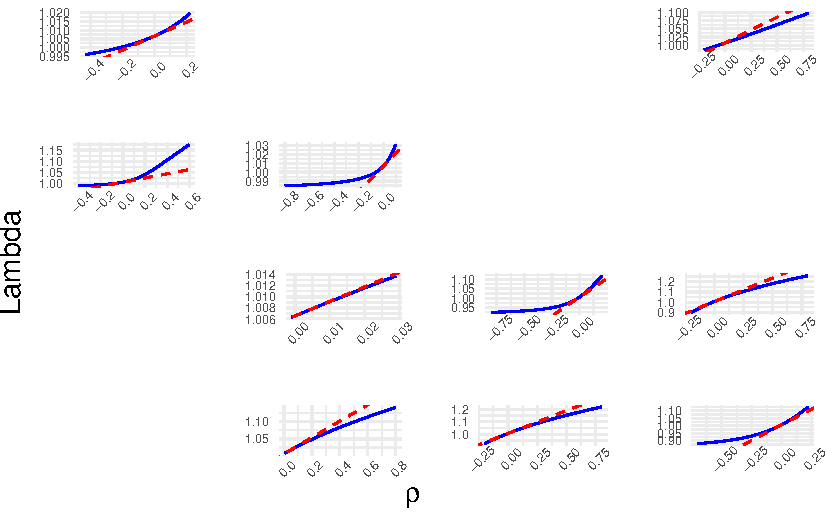
\includegraphics[keepaspectratio]{113-Funciones_de_Transferencia_files/figure-pdf/unnamed-chunk-24-1.pdf}}

\begin{center}\rule{0.5\linewidth}{0.5pt}\end{center}

\bookmarksetup{startatroot}

\chapter{Experimento de Respuesta de Tabla de Vida}\label{ERTV}

Los análisis LTRE (Life Table Response Experiments) permiten descomponer
las diferencias observadas en el crecimiento poblacional entre
poblaciones, tratamientos o periodos de tiempo en contribuciones
demográficas específicas. Este capítulo introduce el enfoque LTRE como
una herramienta retrospectiva para identificar los procesos vitales
responsables de cambios en la dinámica poblacional.

Por: Adriana Ramírez-Martínez y Demetria Mondragón

\section{Experimentos de respuesta de tablas de vida: un enfoque
retrospectivo}\label{experimentos-de-respuesta-de-tablas-de-vida-un-enfoque-retrospectivo}

Los Life Table Response Experiments (LTRE) constituyen un marco
analítico diseñado para explicar \textbf{por qué} dos o más poblaciones,
tratamientos o escenarios difieren en su tasa de crecimiento
poblacional. A diferencia de los análisis prospectivos de sensibilidad y
elasticidad, que evalúan la importancia potencial de cambios hipotéticos
en las tasas vitales, los LTRE son análisis retrospectivos que
cuantifican la contribución real de las diferencias observadas en los
parámetros demográficos.

En este capítulo se presenta el fundamento conceptual de los LTRE,
mostrando cómo las diferencias en matrices de proyección pueden
descomponerse en contribuciones asociadas a transiciones específicas del
ciclo de vida. Se discute la lógica de comparar matrices observadas con
una matriz de referencia y cómo esta elección influye en la
interpretación biológica de los resultados.

Asimismo, se analiza cómo los LTRE permiten identificar qué procesos
demográficos ---como supervivencia, crecimiento o fecundidad--- explican
cambios en el crecimiento poblacional entre condiciones contrastantes.
Este capítulo se diferencia de los anteriores porque desplaza el enfoque
desde la predicción de efectos potenciales hacia la explicación causal
de patrones observados, proporcionando una herramienta clave para
interpretar respuestas poblacionales a variación ambiental, manejo o
perturbaciones. Los LTRE constituyen un puente conceptual entre la
teoría de la dinámica poblacional y su aplicación empírica en estudios
comparativos.

\subsubsection{Librerías de R requeridas para el siguiente
módulo}\label{libreruxedas-de-r-requeridas-para-el-siguiente-muxf3dulo-11}

\begin{Shaded}
\begin{Highlighting}[]
\FunctionTok{library}\NormalTok{(tidyverse)}
\FunctionTok{library}\NormalTok{(Rage)}
\FunctionTok{library}\NormalTok{(DiagrammeR)}
\FunctionTok{library}\NormalTok{(popbio)}
\FunctionTok{library}\NormalTok{(popdemo)}
\FunctionTok{library}\NormalTok{(latex2exp)}
\end{Highlighting}
\end{Shaded}

\section{\texorpdfstring{Introducción a \textbf{Experimento de Respuesta
de Tabla de
Vida}}{Introducción a Experimento de Respuesta de Tabla de Vida}}\label{introducciuxf3n-a-experimento-de-respuesta-de-tabla-de-vida}

La variación en los valores estimados de los parámetros de la matriz son
inherentes a la biología. Esa variación puede ser consecuencia de
múltiples factores individuales y/o de combinaciones, incluyendo efectos
de tiempo, espaciales, genéticos, de tamaño de muestra y por supuesto,
suerte (Hernández et~al., 2024). La variación en los parámetros de la
historia de vida de una especie se pueden evaluar a diferentes niveles:
genético, demográfico, espacial o temporal. En ecología la variación es
la norma ¿Cuál es esta variación? ¿en otra palabras qué es lo que varía?
y ¿cómo los individuos responden a las variables bióticas y abióticas?
son aspectos importantes para determinar la ecología, evolución y
conservación de las especies. La causa de la variación en una población
se puede resumir en tres componentes principales: la genética, el efecto
del ambiente y la interacción entre ambiente y genética (plasticidad
fenotípica) (Sun et~al., 2019; Hastings et~al., 2021). En general se
asume que el tamaño de muestra es lo suficientemente grande para no ser
la causa de la variación, pero dentro de un contexto de dinámica
poblacional las condiciones en las que se encuentran los individuos en
las poblaciones varían, ya sea durante tratamientos manipulados, entre
localidades o periodos de tiempo, y por consecuencia los datos que
colectamos con diferencias en espacio/tiempo también varían y pudieran
tener efecto sobre la matriz de proyección poblacional \(matA\). Por
tanto, las entradas (los parámetros) de esa matriz \textbf{A} variarán
en tiempo/espacio o experimento y esto tendría un impacto sobre la tasa
de crecimiento poblacional \(\lambda\) y en los estimados de dispersión
(Intervalo de confianza o credibilidad); (Caswell, 1989b, 2010).

Tomando en cuenta lo anterior un Experimento de Respuesta de Tabla de
Vida (\textbf{ERTV}) conocido también como \emph{Life Table Response
Experiment} (LTRE, por sus siglas en inglés) descompone la diferencia o
varianza en \emph{λ} entre múltiples poblaciones o tiempo dentro de las
contribuciones de los elementos de la matriz y sus interacciones
(Caswell, 1989a). Entonces al realizar este análisis podemos tener una
apreciación de cómo los cambios en la matriz de datos recolectados en
diferentes tiempos y espacio impactan las tasas vitales y a su vez que
causan cambios en el crecimiento intrínseco \(\lambda\) y otros
parámetros poblacionales (Caswell, 1989a, 2010).

Desde la aplicación del primer ERTV por (Birch, 1953) en su estudio
sobre el efecto de la temperatura, humedad y el alimento sobre tres
especies de escarabajos de harina, las aplicaciones de estos análisis
han sido variadas con diversos fines en las últimas dos décadas
(Caswell, 1989a, 2010). Tanto en diseños fijos en los que se manipulan
uno o más factores, como en diseños aleatorios en los que se analizan
parámetros demográficos en condiciones naturales no manipuladas a lo
largo del tiempo o del espacio (Horvitz, Schemske \& Caswell, 1997;
Teitel, Klimowski \& Campbell, 2016). Los diseños fijos se han utilizado
en poblaciones de animales para investigar las consecuencias
demográficas de la exposición a contaminantes, la manipulación del
alimento o la manipulación de la densidad poblacional (Levin et~al.,
1996; Hansen, Stenseth \& Henttonen, 1999; Oli, Slade \& Dobson, 2001).
En plantas, los análisis ERTV se han utilizado para evaluar las
consecuencias demográficas de la disponibilidad de polinizadores o de la
herbívora, competencia, efectos en intensidades de cosecha y de
fenómenos naturales e inducidos por el humano (Miriti, Joseph Wright \&
Howe, 2001; Garcı́a \& Ehrlén, 2002; Nordbakken, Rydgren \& Økland, 2004;
Mondragón, 2009; Davison et~al., 2010; Gaoue \& Ticktin, 2010; Schmidt
et~al., 2011; Jacquemyn et~al., 2012; Hart-Fredeluces, Ticktin \& Lake,
2021).

Los métodos para calcular los ERTV están constantemente actualizándose y
de acuerdo con (Hernández et~al., 2023) existen 186 análisis de ERTV
para 75 especies de animales y 1487 para 200 especies de plantas. Aunque
en este trabajo no utilizamos la metodología expuesta por dichos autores
mostramos una forma práctica de la aplicación de este análisis.

\subsection{¿Cómo se diferencia la elasticidad de
ERTV?}\label{cuxf3mo-se-diferencia-la-elasticidad-de-ertv}

A diferencia de la elasticidad, la cual es un tipo de análisis de
perturbación que examina cuánto cambiaría el crecimiento de la población
si se cambiaran una de las entradas de la matriz comparando múltiples
matrices, el análisis ERTV examina cuánto cambio hay en \(\lambda\) en
función de la variación observada en las entradas de la matriz (Caswell,
1989b, 2010; Horvitz, Schemske \& Caswell, 1997); y por consecuencia es
un análisis que toma en cuenta el cambio de las variaciones
individualmente registradas en matrices en diferentes poblaciones/
tiempo / experimentos, etc. (Caswell, 2010). Nota que ERTV es una
herramienta suplementaria para evaluar el efecto de perturbaciones como
los de elasticidad (Caswell, 1989a), dinámica de transiciones (Stott,
Townley \& Hodgson, 2011) y funciones de transferencias (Stott, Hodgson
\& Townley, 2012a) y no un reemplazo. Cada una de estas herramientas
tiene un propósito y una interpretación diferente con sus supuestos.

\begin{tcolorbox}[enhanced jigsaw, arc=.35mm, bottomrule=.15mm, bottomtitle=1mm, breakable, colback=white, colbacktitle=quarto-callout-important-color!10!white, colframe=quarto-callout-important-color-frame, coltitle=black, left=2mm, leftrule=.75mm, opacityback=0, opacitybacktitle=0.6, rightrule=.15mm, title=\textcolor{quarto-callout-important-color}{\faExclamation}\hspace{0.5em}{Importante}, titlerule=0mm, toprule=.15mm, toptitle=1mm]

\textbf{Dos preguntas distintas, dos herramientas distintas.}

\begin{itemize}
\tightlist
\item
  \textbf{Elasticidad (prospectiva):} ¿Qué pasaría con λ si
  modificáramos hipotéticamente una entrada de la matriz?
\item
  \textbf{LTRE (retrospectivo):} Dadas las diferencias observadas entre
  dos matrices, ¿cuáles entradas explican la diferencia en λ?
\end{itemize}

LTRE es \textbf{complementario}, no sustituto, de elasticidad. Cuando la
elasticidad de un parámetro es alta pero la varianza observada es baja,
ese parámetro contribuye poco al LTRE. Cuando la elasticidad es modesta
pero la varianza es grande, ese parámetro puede dominar el LTRE. Las dos
métricas pueden señalar resultados distintos, y ambos son útiles.

\end{tcolorbox}

\section{Formulación y cálculo de los
LTRE}\label{formulaciuxf3n-y-cuxe1lculo-de-los-ltre}

A continuación se describe la formulación matemática de los LTRE y su
implementación computacional para descomponer diferencias en el
crecimiento poblacional. A diferencia del análisis de elasticidad
poblacional, los LTRE explican diferencias observadas en lugar de
evaluar cambios hipotéticos en los parámetros demográficos. Las
contribuciones LTRE pueden descomponerse en términos de matrices
\textbf{U} y \textbf{F}, introducidas en el capítulo de
\hyperref[MatricesTFC]{Matrices U, F y C}.

\begin{center}\rule{0.5\linewidth}{0.5pt}\end{center}

\section{Métodos}\label{muxe9todos}

\subsection{Ejemplo práctico de ERTV}\label{ejemplo-pruxe1ctico-de-ertv}

Para ejemplificar el cálculo de los ERTV utilizaremos los datos
recabados por Ramírez-Martínez colectados de 2017 a 2018 para la
orquídea epífita \emph{Oncidium brachyandrum} Lindl. en un bosque de
encino estacional en Oaxaca, México (Ramı́rez Martı́nez, 2021). La
pregunta principal del estudio era saber qué tasas vitales estaban
ligadas a las variaciones en los valores de λ de poblaciones de \emph{O.
brachyandrum} creciendo sobre dos hospederos \emph{Quercus martinezii}
C.H.Mull. y \emph{Q. rugosa} Née. Usando el método ERTV se pudo evaluar
el efecto que tiene la variación observada en los parámetros de las
matrices en función de las especies de hospedero en los que se
encontraban creciendo.

Como el ERTV es una forma de análisis retrospectivo y es análogo al
ANOVA (porque cuantifica los efectos observados de los elementos
individuales de matriz sobre la variación observada en \emph{λ}, en
contraposición a los efectos esperados) se requiere de un valor de
referencia para realizar las comparaciones, por lo que se toma la matriz
con el valor más alto de \emph{λ} como valor de referencia (Caswell,
2010; Timsina et~al., 2021).

\begin{tcolorbox}[enhanced jigsaw, arc=.35mm, bottomrule=.15mm, bottomtitle=1mm, breakable, colback=white, colbacktitle=quarto-callout-tip-color!10!white, colframe=quarto-callout-tip-color-frame, coltitle=black, left=2mm, leftrule=.75mm, opacityback=0, opacitybacktitle=0.6, rightrule=.15mm, title=\textcolor{quarto-callout-tip-color}{\faLightbulb}\hspace{0.5em}{Recomendación}, titlerule=0mm, toprule=.15mm, toptitle=1mm]

\textbf{Cómo elegir la matriz de referencia.}

El método de Caswell descompone la diferencia
\(\lambda^{(i)} - \lambda^{(\text{ref})}\) usando sensibilidades
evaluadas en la \textbf{matriz promedio} entre la condición \(i\) y la
condición de referencia. Hay tres opciones comunes para la matriz de
referencia:

\begin{itemize}
\tightlist
\item
  \textbf{Matriz con λ más alto:} útil cuando se quiere identificar qué
  procesos \emph{limitan} el crecimiento en las otras condiciones (esta
  es la opción usada en este ejemplo).
\item
  \textbf{Matriz control:} apropiado en diseños experimentales con
  tratamientos vs.~control.
\item
  \textbf{Matriz promedio:} útil cuando no hay un escenario ``mejor''
  obvio y se quiere descomponer la varianza simétricamente.
\end{itemize}

La elección de referencia afecta el signo de las contribuciones (no su
magnitud relativa), así que conviene declararla explícitamente al
reportar resultados.

\end{tcolorbox}

A continuación, se muestran dos matrices de tipo Lefkovitch (matrices
construidas con base en estadíos) para las poblaciones de \emph{O.
brachyandrum} y sus valores respectivos de λ en los dos hospederos, A)
\emph{Q. martinezii} (λ=1.3; IC: 1.11-1.45) y B) \emph{Q. rugosa}
(λ=0.98; IC: 0.87-0.99). El valor de λ fue mayor en \emph{Q. martinezii}
por lo que la matriz de esta especie fue la matriz de referencia para
calcular los ERTV.

\textbf{A)}

{\def\LTcaptype{none} % do not increment counter
\begin{longtable}[]{@{}lllll@{}}
\toprule\noalign{}
& Plántula & Infantil & Juvenil & Adulto \\
\midrule\noalign{}
\endhead
\bottomrule\noalign{}
\endlastfoot
Plántula & 0.68 & 0.02 & 3.88 & 16.53 \\
Infantil & 0.23 & 0.75 & 0.23 & 0 \\
Juvenil & 0 & 0.13 & 0.53 & 0.58 \\
Adulto & 0 & 0 & 0.17 & 0.38 \\
\end{longtable}
}

\textbf{B)}

{\def\LTcaptype{none} % do not increment counter
\begin{longtable}[]{@{}lllll@{}}
\toprule\noalign{}
& Plántula & Infantil & Juvenil & Adulto \\
\midrule\noalign{}
\endhead
\bottomrule\noalign{}
\endlastfoot
Plántula & 0.64 & 0.06 & 0 & 0.005 \\
Infantil & 0.23 & 0.75 & 0.27 & 0 \\
Juvenil & 0 & 0.08 & 0.47 & 0.27 \\
Adulto & 0 & 0 & 0.27 & 0.68 \\
\end{longtable}
}

\begin{center}\rule{0.5\linewidth}{0.5pt}\end{center}

\subsection{Matrices de proyecciones y ciclo de vida por especie de
hospedero}\label{matrices-de-proyecciones-y-ciclo-de-vida-por-especie-de-hospedero}

Cuadro 1. Matrices de proyección poblaciones de dos poblaciones de
\emph{Oncidiun brachyandrum} creciendo sobre \emph{Quercus martinezii} y
\emph{Q. rugosa}. Los valores de λ (intervalos de confianza ± 95\%) son
mostrados en la parte superior izquierda de cada matriz, \emph{qx},
mortalidad por estadío; \emph{w}, categorías estables de tamaño por
estadío; valor reproductivo por estadío, \emph{n} = el tamaño de muestra
en el tiempo cero (el primer muestreo). p: plántula, i: infantil, j:
juvenil, A; adulto (Ramı́rez Martı́nez, 2021). Los valores en negritas son
los valores que representan la proporción de individuos que se queda en
ese estadio.

\begin{figure}[H]

{\centering \pandocbounded{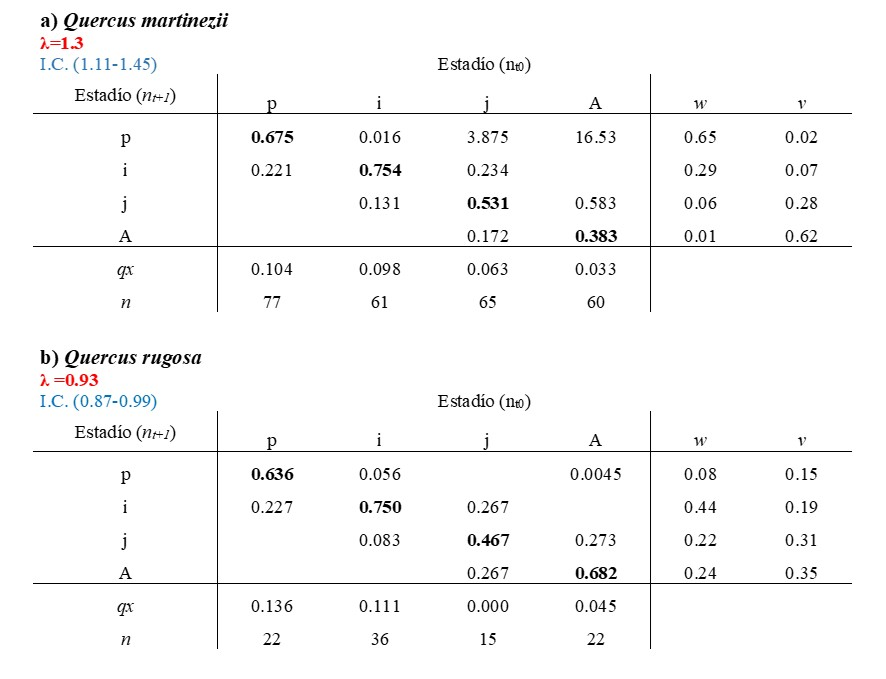
\includegraphics[keepaspectratio,alt={Tabla comparativa con dos matrices de transición poblacional de Oncidium brachyandrum sobre dos especies de roble; cada matriz muestra tasas de transición entre estadios plántula, infantil, juvenil y adulto, junto con sus parámetros derivados (lambda, mortalidad, estructura estable, valor reproductivo, tamaño de muestra)}]{images/Imagen1.jpg}}

}

\caption{Cuadro 1. Matrices de proyección poblacional de \emph{Oncidium
brachyandrum} en dos hospederos (\emph{Quercus martinezii} y \emph{Q.
rugosa}), con λ e intervalos de confianza, mortalidad q\_x, categorías
estables w, valor reproductivo y tamaño de muestra inicial}

\end{figure}%

\begin{center}\rule{0.5\linewidth}{0.5pt}\end{center}

\subsection{Diagrama del ciclo de
vida}\label{diagrama-del-ciclo-de-vida}

\subsection{\texorpdfstring{Diagrama para \emph{Quercus
martinezii}}{Diagrama para Quercus martinezii}}\label{diagrama-para-quercus-martinezii}

Primeramente se creó el ciclo de vida por especie de hospedero
utilizando el siguiente código:

\begin{Shaded}
\begin{Highlighting}[]
\NormalTok{matmart }\OtherTok{\textless{}{-}} \FunctionTok{rbind}\NormalTok{(}
  \FunctionTok{c}\NormalTok{(}\FloatTok{0.68}\NormalTok{, }\FloatTok{0.02}\NormalTok{, }\FloatTok{3.88}\NormalTok{, }\FloatTok{16.53}\NormalTok{),}
  \FunctionTok{c}\NormalTok{(}\FloatTok{0.22}\NormalTok{, }\FloatTok{0.76}\NormalTok{, }\FloatTok{0.23}\NormalTok{, }\FloatTok{0.0}\NormalTok{),}
  \FunctionTok{c}\NormalTok{(}\FloatTok{0.0}\NormalTok{, }\FloatTok{0.13}\NormalTok{, }\FloatTok{0.53}\NormalTok{, }\FloatTok{0.58}\NormalTok{),}
  \FunctionTok{c}\NormalTok{(}\FloatTok{0.0}\NormalTok{, }\FloatTok{0.0}\NormalTok{, }\FloatTok{0.17}\NormalTok{, }\FloatTok{0.38}\NormalTok{)}
\NormalTok{)}

\FunctionTok{colSums}\NormalTok{(matmart) }\CommentTok{\# sumar las filas de la matriz}
\end{Highlighting}
\end{Shaded}

\begin{verbatim}
[1]  0.90  0.91  4.81 17.49
\end{verbatim}

\begin{Shaded}
\begin{Highlighting}[]
\NormalTok{stages }\OtherTok{\textless{}{-}} \FunctionTok{c}\NormalTok{(}\StringTok{"plántula"}\NormalTok{, }\StringTok{"infantil"}\NormalTok{, }\StringTok{"juvenil"}\NormalTok{, }\StringTok{"adulto"}\NormalTok{) }\CommentTok{\# asignar los nombres de los estadíos}
\NormalTok{title }\OtherTok{\textless{}{-}} \ConstantTok{NULL} \CommentTok{\# título del diagrama ninguno}
\NormalTok{graph }\OtherTok{\textless{}{-}} \FunctionTok{expand.grid}\NormalTok{(}\AttributeTok{to =}\NormalTok{ stages, }\AttributeTok{from =}\NormalTok{ stages) }\CommentTok{\# crear un data frame con los estadíos}
\NormalTok{graph}\SpecialCharTok{$}\NormalTok{trans }\OtherTok{\textless{}{-}} \FunctionTok{round}\NormalTok{(}\FunctionTok{c}\NormalTok{(matmart), }\DecValTok{4}\NormalTok{) }\CommentTok{\# redondear los valores de la matriz a 4 decimales}
\NormalTok{graph }\OtherTok{\textless{}{-}}\NormalTok{ graph[graph}\SpecialCharTok{$}\NormalTok{trans }\SpecialCharTok{\textgreater{}} \DecValTok{0}\NormalTok{, ] }\CommentTok{\# seleccionar solo los valores mayores a 0}
\NormalTok{nodes }\OtherTok{\textless{}{-}} \FunctionTok{paste}\NormalTok{(}\FunctionTok{paste0}\NormalTok{(}\StringTok{"\textquotesingle{}"}\NormalTok{, stages, }\StringTok{"\textquotesingle{}"}\NormalTok{), }\AttributeTok{collapse =} \StringTok{"; "}\NormalTok{) }\CommentTok{\# crear los nodos}
\NormalTok{graph}\SpecialCharTok{$}\NormalTok{min\_len }\OtherTok{\textless{}{-}}\NormalTok{ (}\FunctionTok{as.numeric}\NormalTok{(graph}\SpecialCharTok{$}\NormalTok{to) }\SpecialCharTok{{-}} \FunctionTok{as.numeric}\NormalTok{(graph}\SpecialCharTok{$}\NormalTok{from)) }\SpecialCharTok{*} \DecValTok{4} \CommentTok{\# calcular la longitud de las flechas}
\end{Highlighting}
\end{Shaded}

\pandocbounded{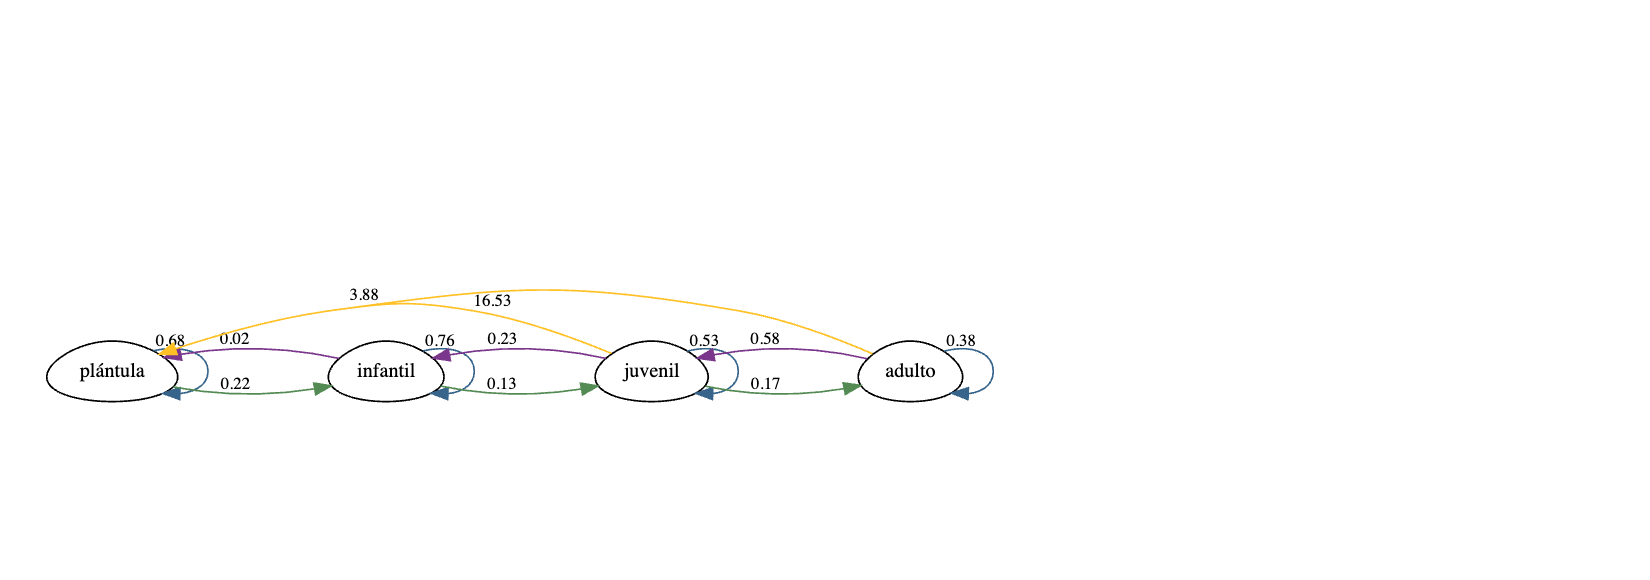
\includegraphics[keepaspectratio]{114-LTRE_files/figure-pdf/LTRE2-1.png}}

\vspace{-5truemm}

El ciclo de vida de \emph{Oncidium brachyandrum} creciendo sobre
\emph{Quercus martinezii}. Las flechas representan las transiciones
entre estadíos, estasis y fecundidades, y los números son las tasas
vitales de fecundidad, supervivencia y crecimiento. El color
\text{\textcolor[HTML]{FFC125}{amarillo}} para fecundidad,
\text{\textcolor[HTML]{36648B}{azul}} para supervivencia,
\text{\textcolor[HTML]{548B54}{verde}} para crecimiento,
\text{\textcolor[HTML]{7A378B}{violeta}} para retroceso y
\text{\textcolor[HTML]{36648B}{azul oscuro}} para permanencia.

\begin{center}\rule{0.5\linewidth}{0.5pt}\end{center}

\subsection{\texorpdfstring{Diagrama para \emph{Quercus
rugosa}}{Diagrama para Quercus rugosa}}\label{diagrama-para-quercus-rugosa}

\begin{Shaded}
\begin{Highlighting}[]
\NormalTok{matrug }\OtherTok{\textless{}{-}} \FunctionTok{rbind}\NormalTok{(}
  \FunctionTok{c}\NormalTok{(}\FloatTok{0.64}\NormalTok{, }\FloatTok{0.06}\NormalTok{, }\DecValTok{0}\NormalTok{, }\FloatTok{0.0045}\NormalTok{),}
  \FunctionTok{c}\NormalTok{(}\FloatTok{0.27}\NormalTok{, }\FloatTok{0.75}\NormalTok{, }\FloatTok{0.27}\NormalTok{, }\FloatTok{0.0}\NormalTok{),}
  \FunctionTok{c}\NormalTok{(}\FloatTok{0.0}\NormalTok{, }\FloatTok{0.08}\NormalTok{, }\FloatTok{0.47}\NormalTok{, }\FloatTok{0.28}\NormalTok{),}
  \FunctionTok{c}\NormalTok{(}\FloatTok{0.0}\NormalTok{, }\FloatTok{0.0}\NormalTok{, }\FloatTok{0.27}\NormalTok{, }\FloatTok{0.68}\NormalTok{))}

\NormalTok{stages }\OtherTok{\textless{}{-}} \FunctionTok{c}\NormalTok{(}\StringTok{"plántula"}\NormalTok{, }\StringTok{"infantil"}\NormalTok{, }\StringTok{"juvenil"}\NormalTok{, }\StringTok{"adulto"}\NormalTok{)}
\NormalTok{title }\OtherTok{\textless{}{-}} \ConstantTok{NULL}
\NormalTok{graph }\OtherTok{\textless{}{-}} \FunctionTok{expand.grid}\NormalTok{(}\AttributeTok{to =}\NormalTok{ stages, }\AttributeTok{from =}\NormalTok{ stages)}
\NormalTok{graph}\SpecialCharTok{$}\NormalTok{trans }\OtherTok{\textless{}{-}} \FunctionTok{round}\NormalTok{(}\FunctionTok{c}\NormalTok{(matrug), }\DecValTok{4}\NormalTok{)}
\NormalTok{graph }\OtherTok{\textless{}{-}}\NormalTok{ graph[graph}\SpecialCharTok{$}\NormalTok{trans }\SpecialCharTok{\textgreater{}} \DecValTok{0}\NormalTok{, ]}
\NormalTok{nodes }\OtherTok{\textless{}{-}} \FunctionTok{paste}\NormalTok{(}\FunctionTok{paste0}\NormalTok{(}\StringTok{"\textquotesingle{}"}\NormalTok{, stages, }\StringTok{"\textquotesingle{}"}\NormalTok{), }\AttributeTok{collapse =} \StringTok{"; "}\NormalTok{)}
\NormalTok{graph}\SpecialCharTok{$}\NormalTok{min\_len }\OtherTok{\textless{}{-}}\NormalTok{ (}\FunctionTok{as.numeric}\NormalTok{(graph}\SpecialCharTok{$}\NormalTok{to) }\SpecialCharTok{{-}} \FunctionTok{as.numeric}\NormalTok{(graph}\SpecialCharTok{$}\NormalTok{from)) }\SpecialCharTok{*} \DecValTok{4}
\NormalTok{graph}\SpecialCharTok{$}\NormalTok{col }\OtherTok{\textless{}{-}} \FunctionTok{c}\NormalTok{(}
\StringTok{"steelblue4"}\NormalTok{, }\StringTok{"PaleGreen4"}\NormalTok{, }\StringTok{"MediumOrchid4"}\NormalTok{, }\StringTok{"steelblue4"}\NormalTok{, }\StringTok{"PaleGreen4"}\NormalTok{, }\StringTok{"MediumOrchid4"}\NormalTok{,}\StringTok{"steelblue4"}\NormalTok{, }\StringTok{"PaleGreen4"}\NormalTok{,  }\StringTok{"Goldenrod1"}\NormalTok{, }\StringTok{"MediumOrchid4"}\NormalTok{, }\StringTok{"steelblue4"}
\NormalTok{)}
\NormalTok{edges }\OtherTok{\textless{}{-}} \FunctionTok{paste0}\NormalTok{(}\StringTok{"\textquotesingle{}"}\NormalTok{, graph}\SpecialCharTok{$}\NormalTok{from, }\StringTok{"\textquotesingle{}"}\NormalTok{, }\StringTok{" {-}\textgreater{} "}\NormalTok{, }\StringTok{"\textquotesingle{}"}\NormalTok{, graph}\SpecialCharTok{$}\NormalTok{to, }\StringTok{"\textquotesingle{}"}\NormalTok{,}
                \StringTok{"[minlen="}\NormalTok{, graph}\SpecialCharTok{$}\NormalTok{min\_len,}
                \StringTok{",fontsize="}\NormalTok{, }\DecValTok{10}\NormalTok{,}
                \StringTok{",color="}\NormalTok{, graph}\SpecialCharTok{$}\NormalTok{col,}
                \StringTok{",xlabel="}\NormalTok{, }\FunctionTok{paste}\NormalTok{(}\StringTok{"}\SpecialCharTok{\textbackslash{}"}\StringTok{"}\NormalTok{, graph}\SpecialCharTok{$}\NormalTok{trans),}
                \StringTok{"}\SpecialCharTok{\textbackslash{}"}\StringTok{]}\SpecialCharTok{\textbackslash{}n}\StringTok{"}\NormalTok{,}
                \AttributeTok{collapse =} \StringTok{""}
\NormalTok{)}
\FunctionTok{grViz}\NormalTok{(}
  \FunctionTok{paste}\NormalTok{(}
    \StringTok{"}
\StringTok{digraph \{}
\StringTok{  \{}
\StringTok{    graph[overlap=false];}
\StringTok{    rank=same;}
\StringTok{    node [shape="}\NormalTok{, }\StringTok{"egg"}\NormalTok{, }\StringTok{", fontsize="}\NormalTok{, }\DecValTok{12}\NormalTok{, }\StringTok{"];"}\NormalTok{,}
\NormalTok{    nodes, }\StringTok{"}
\StringTok{  \}"}\NormalTok{,}
    \StringTok{"ordering=out}
\StringTok{  x [style=invis]}
\StringTok{  x {-}\textgreater{} \{"}\NormalTok{, nodes, }\StringTok{"\} [style=invis]"}\NormalTok{, edges,}
    \StringTok{"labelloc=}\SpecialCharTok{\textbackslash{}"}\StringTok{t}\SpecialCharTok{\textbackslash{}"}\StringTok{;}
\StringTok{  label=}\SpecialCharTok{\textbackslash{}"}\StringTok{"}\NormalTok{, title, }\StringTok{"}\SpecialCharTok{\textbackslash{}"}
\StringTok{\}"}
\NormalTok{  )}
\NormalTok{)}
\end{Highlighting}
\end{Shaded}

\pandocbounded{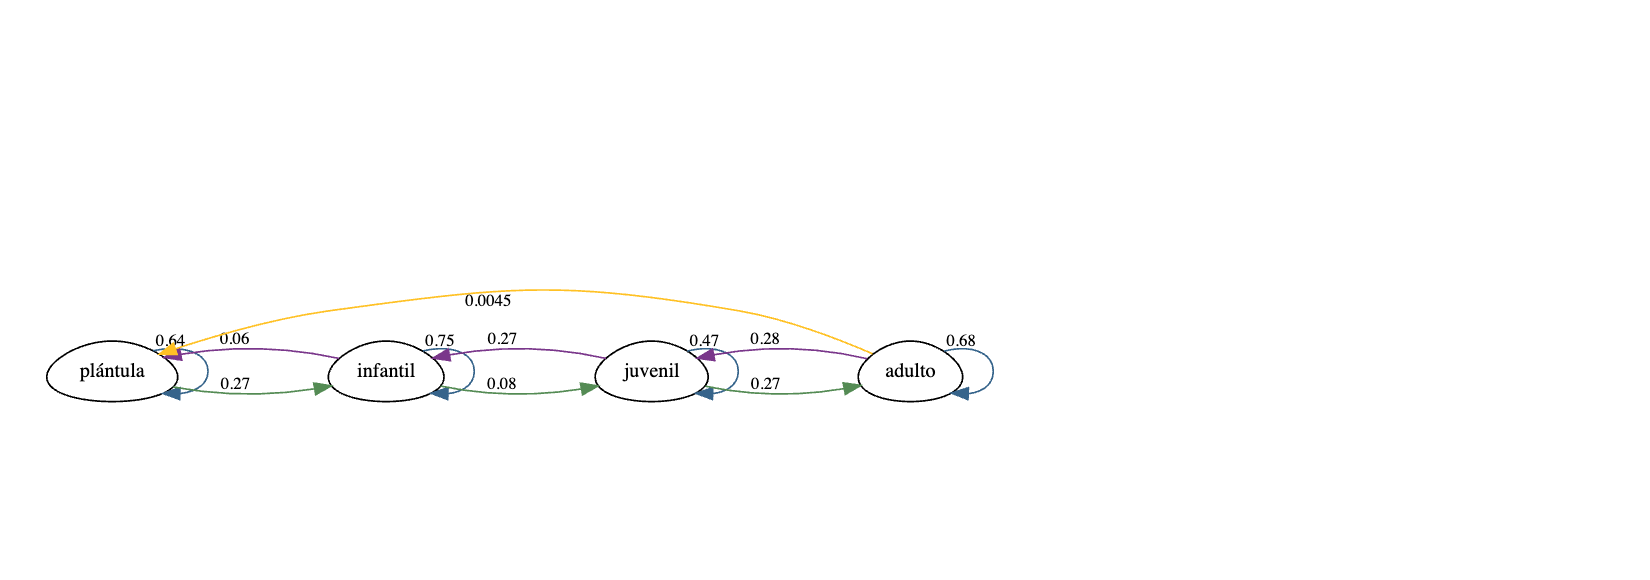
\includegraphics[keepaspectratio]{114-LTRE_files/figure-pdf/LTRE3_Quercus_rugosa-1.png}}

El ciclo de vida de \emph{Oncidium brachyandrum} creciendo sobre
\emph{Quercus rugosa}. Las flechas representan las transiciones entre
estadíos, estasis y fecundidades, y los números son las tasas vitales de
fecundidad, supervivencia y crecimiento. El color {amarillo} para
fecundidad, {azul} para supervivencia, {verde} para crecimiento,
{violeta} para retroceso y {azul oscuro} para permanencia.

\begin{center}\rule{0.5\linewidth}{0.5pt}\end{center}

\section{Procedimiento para ERTV en
Excel}\label{procedimiento-para-ertv-en-excel}

Para facilitar el entendimiento de cómo se calcula ERTV se creó la
matriz con los términos de referencia (Cuadro 1).

{\def\LTcaptype{none} % do not increment counter
\begin{longtable}[]{@{}
  >{\raggedright\arraybackslash}p{(\linewidth - 8\tabcolsep) * \real{0.2000}}
  >{\raggedright\arraybackslash}p{(\linewidth - 8\tabcolsep) * \real{0.2000}}
  >{\raggedright\arraybackslash}p{(\linewidth - 8\tabcolsep) * \real{0.2000}}
  >{\raggedright\arraybackslash}p{(\linewidth - 8\tabcolsep) * \real{0.2000}}
  >{\raggedright\arraybackslash}p{(\linewidth - 8\tabcolsep) * \real{0.2000}}@{}}
\toprule\noalign{}
\begin{minipage}[b]{\linewidth}\raggedright
Estadío
\end{minipage} & \begin{minipage}[b]{\linewidth}\raggedright
Plántulas (1)
\end{minipage} & \begin{minipage}[b]{\linewidth}\raggedright
Infantiles (2)
\end{minipage} & \begin{minipage}[b]{\linewidth}\raggedright
Juveniles (3)
\end{minipage} & \begin{minipage}[b]{\linewidth}\raggedright
Adultos (4)
\end{minipage} \\
\midrule\noalign{}
\endhead
\bottomrule\noalign{}
\endlastfoot
Plántulas (1) & p\textsubscript{11} (permanencia de plántulas) &
g\textsubscript{21} (retroceso de infantiles a plántulas) &
f\textsubscript{31} (plántulas generadas)g\textsubscript{31} (retroceso
de juveniles a plántulas) & f\textsubscript{41} (plántulas generadas) \\
Infantiles (2) & g\textsubscript{12} (crecimiento de plántulas a
infantiles) & p\textsubscript{22} (permanencia de infantiles) &
g\textsubscript{32} (retroceso de juveniles a infantiles) &
g\textsubscript{42} (retroceso de adultos a infantiles) \\
Juveniles (3) & g\textsubscript{13} (crecimiento de plántulas a
juveniles) & g\textsubscript{23} (crecimiento de infantiles a juveniles)
& p\textsubscript{33} (permanencia de juveniles) & g\textsubscript{43}
(retroceso de adultos a juveniles) \\
Adultos (4) & g\textsubscript{14} (crecimiento de plántulas a adultos) &
g\textsubscript{24} (crecimiento de infantiles a adultos) &
g\textsubscript{34} (crecimiento de juveniles a adultos) &
p\textsubscript{44} (permanencia de adultos) \\
Supervivencia & s\textsubscript{1} (de plántulas) & s\textsubscript{2}
(de infantiles) & s\textsubscript{3} (de juveniles) & s\textsubscript{4}
(de adultos) \\
\end{longtable}
}

\textbf{Cuadro 1.} Matriz de términos para el entendimiento de los ERTV.
Donde: f= fecundidad, g= crecimiento o retrogresión, p= permanencia y
s=supervivencia. Los subíndices se refieren a las transiciones entre
estadíos.Nota que los parámetros de juvenil que retrogresan a plántula y
esa etapa produciendo plántulas se suman.

En la sección \textbf{Apéndice C} se encuentra una hoja de Excel para
poder realizar los cálculos de ERTV. En esta sección se explica cómo se
construye la matriz de términos y cómo se calculan las tasas vitales
para cada una de las especies de hospedero.

Una vez colocadas las matrices en la hoja de trabajo el primer paso será
sumar las columnas para cada estadio, esto significará la supervivencia
(s) por estadío (s\textsubscript{1}, s\textsubscript{2},
s\textsubscript{3}, s\textsubscript{4}); para el caso de \emph{Q.
martinezii} en plántulas sería s\textsubscript{1}= 0.68+0.22= 0.90
(Figura 3). Después se tienen que calcular las transiciones con respecto
a la supervivencia; por lo que para el caso de la transición
g\textsubscript{12} para la matriz de \emph{Q. martinezii} tenemos
g\textsubscript{12}= 0.22/0.90=0.25; este cálculo se realiza para todas
las transiciones. Los valores de fecundidad (f) se tomarán tal cual de
la matriz de fecundidad \(matF\). Una vez obtenido esto se procederá a
realizar los cálculos con las ecuaciones que se muestran del lado
derecho para cada una de las celdas y, además, esto nos sirve para
verificar que hayamos calculado bien cada una de las tasas vitales. Por
ejemplo, observamos que una proporción de plántulas en \emph{Q.
martinezii} se mantuvo (0.67) este valor se obtiene de multiplicar la
supervivencia de plántulas (s\textsubscript{1}) por la sustracción de 1
menos el crecimiento de plántulas a infantiles 0.89 (1-0.25) = 0.68
(ecuación s\textsubscript{1}* (1-g\textsubscript{12})).

\begin{center}\rule{0.5\linewidth}{0.5pt}\end{center}

\subsection{Método usando Excel}\label{muxe9todo-usando-excel}

En un archivo nuevo de Excel se arma la base, con la columna de
vital\_rate al principio, seguido por las especies de hospederos
(tratamientos) poniendo primeramente el control y después la columna de
matrix. Esta base contendrá las ecuaciones de la matriz de referencia.
Como la matriz de \emph{Q. martinezii} tuvo los valores más altos de
lambda está se colocará primero en nuestra base que utilizaremos para
correr el análisis ERTV.

\begin{verbatim}
Error in `flextable()`:
! could not find function "flextable"
\end{verbatim}

\textbf{Cuadro 2.} Ejemplo de base para poder calcular los ERTV.

Es importante colocar en la segunda fila la palabra lambda en la primera
columna y después los valores según corresponda a cada tratamiento.
Debido a que en \emph{Q. rugosa} no hubo producción de plántulas
(f\textsubscript{31}) pero en \emph{Q. martinezii} si hubo se coloca una
cantidad muy pequeña pero mayor a cero (e.g.~0.00001) para que se pueda
correr el análisis, para las otras transiciones en valor puede ser 0.
Una vez culminada la base se guarda el archivo en formato de texto, para
continuar en R. Es importante comenzar a colocar las ecuaciones a partir
de la segunda fila en la columna matrix.

\begin{tcolorbox}[enhanced jigsaw, arc=.35mm, bottomrule=.15mm, bottomtitle=1mm, breakable, colback=white, colbacktitle=quarto-callout-warning-color!10!white, colframe=quarto-callout-warning-color-frame, coltitle=black, left=2mm, leftrule=.75mm, opacityback=0, opacitybacktitle=0.6, rightrule=.15mm, title=\textcolor{quarto-callout-warning-color}{\faExclamationTriangle}\hspace{0.5em}{Advertencia}, titlerule=0mm, toprule=.15mm, toptitle=1mm]

\textbf{Una tasa vital observada en cero requiere un manejo especial.}
El método LTRE asume que las tasas vitales están definidas y son
comparables entre matrices. Si una tasa es 0 en una condición pero
positiva en otra (e.g., en el ejemplo \emph{Q. rugosa} no produjo
plántulas), el cálculo numérico puede fallar o producir contribuciones
engañosas. Una solución práctica es reemplazar el 0 por un valor muy
pequeño (e.g., 0.00001), pero hay que reconocer que esto introduce
sesgo. Una alternativa más robusta es estimar la tasa vital con métodos
bayesianos (ver capítulo de
\hyperref[acercamiento-bayesiano-para-calcular-transiciones-y-fecundidades]{Acercamiento
bayesiano}), que evitan ceros exactos y producen distribuciones
posteriores apropiadas para LTRE.

\end{tcolorbox}

\begin{center}\rule{0.5\linewidth}{0.5pt}\end{center}

\section{Procedimiento en R}\label{procedimiento-en-r}

Subir la base de datos de la carpeta de trabajo y cargarla en R.

\begin{itemize}
\tightlist
\item
  Nota que debería observar la base de datos en la consola de R para
  verificar que se haya cargado correctamente con los mismos valores que
  en la hoja de Excel.
\end{itemize}

\begin{Shaded}
\begin{Highlighting}[]
\CommentTok{\# Asegurarse de tener instalado y cargado el paquete \textquotesingle{}popbio\textquotesingle{} package }

\CommentTok{\# oncidium\textless{}{-}read.table("data/vitalratesoncidium.txt", sep="\textbackslash{}t", header=TRUE, stringsAsFactors=FALSE, fill=TRUE) }
     \CommentTok{\# Aqui la alternativa si tiene los datos en una hoja de Excel}

\CommentTok{\#oncidium }

\NormalTok{Oncidium}
\end{Highlighting}
\end{Shaded}

\begin{verbatim}
# A tibble: 17 x 4
   names.vitalrate martinezzi  rugosa matrix          
   <chr>                <dbl>   <dbl> <chr>           
 1 lambda              1.3     0.93   ""              
 2 s1                  0.896   0.864  "s1*(1-g12)"    
 3 g12                 0.246   0.263  "s1*g12"        
 4 s2                  0.902   0.889  "0"             
 5 g21                 0.0182  0.0625 "0"             
 6 g23                 0.145   0.0937 "s2*g21"        
 7 s3                  0.938   1.000  "s2*(1-g23-g21)"
 8 g32                 0.25    0.267  "s2*g23"        
 9 g34                 0.183   0.267  "0"             
10 s4                  0.967   0.955  "f31"           
11 g43                 0.603   0.286  "s3*g32"        
12 f31                 3.88    0.0001 "s3*(1-g34-g32)"
13 f41                16.5     0.0045 "s3*g34"        
14 <NA>               NA      NA      "f41"           
15 <NA>               NA      NA      "0"             
16 <NA>               NA      NA      "s4*g43"        
17 <NA>               NA      NA      "s4*(1-g43)"    
\end{verbatim}

Debido a que la columna de matriz contiene más filas con datos nos
aparecerá la leyenda NA en las otras columnas esto se refiere a que no
hay valores disponibles para esas filas

Para extraer los nombres de las tasas vitales (de la fila 2 a la 13),
sin incluir el valor de \(\lambda\) el cual está en la primera

\begin{Shaded}
\begin{Highlighting}[]
\NormalTok{razonvital }\OtherTok{\textless{}{-}}\NormalTok{ Oncidium}\SpecialCharTok{$}\NormalTok{names.vitalrate[}\DecValTok{2}\SpecialCharTok{:}\DecValTok{13}\NormalTok{]}

\NormalTok{razonvital }\CommentTok{\# mostrar los nombres del objeto razón vital}
\end{Highlighting}
\end{Shaded}

\begin{verbatim}
 [1] "s1"  "g12" "s2"  "g21" "g23" "s3"  "g32" "g34" "s4"  "g43" "f31" "f41"
\end{verbatim}

\begin{center}\rule{0.5\linewidth}{0.5pt}\end{center}

\subsection{\texorpdfstring{Tasa vital sobre \emph{Q.
martinezii}}{Tasa vital sobre Q. martinezii}}\label{tasa-vital-sobre-q.-martinezii}

Extraer tasas vitales de la orquídea \emph{Oncidium brachyandrum} que
crecen sobre \emph{Q. martinezii} y dejar a lambda a un lado

\begin{Shaded}
\begin{Highlighting}[]
\NormalTok{Martinezzi }\OtherTok{\textless{}{-}}\NormalTok{ Oncidium}\SpecialCharTok{$}\NormalTok{martinezzi[}\DecValTok{2}\SpecialCharTok{:}\DecValTok{13}\NormalTok{] }\CommentTok{\# [2:13] se refiere a la fila 2 hasta la 13.}
\FunctionTok{names}\NormalTok{(Martinezzi) }\OtherTok{\textless{}{-}}\NormalTok{ razonvital }\CommentTok{\# asignar los nombres de las tasas vitales}
\NormalTok{Martinezzi}
\end{Highlighting}
\end{Shaded}

\begin{verbatim}
         s1         g12          s2         g21         g23          s3 
 0.89610000  0.24637681  0.90163934  0.01818182  0.14545450  0.93750000 
        g32         g34          s4         g43         f31         f41 
 0.25000000  0.18333300  0.96666700  0.60344800  3.87500000 16.53000000 
\end{verbatim}

\begin{center}\rule{0.5\linewidth}{0.5pt}\end{center}

\subsection{\texorpdfstring{Tasa vital sobre \emph{Q.
rugosa}}{Tasa vital sobre Q. rugosa}}\label{tasa-vital-sobre-q.-rugosa}

Extraer tasas vitales de la orquídea \emph{Oncidium brachyandrum} que
crecen sobre \emph{Q. rugosa} y dejar a lambda a un lado.

\begin{Shaded}
\begin{Highlighting}[]
\NormalTok{Rugosa }\OtherTok{\textless{}{-}}\NormalTok{ Oncidium}\SpecialCharTok{$}\NormalTok{rugosa[}\DecValTok{2}\SpecialCharTok{:}\DecValTok{13}\NormalTok{]}
\FunctionTok{names}\NormalTok{(Rugosa) }\OtherTok{\textless{}{-}}\NormalTok{ razonvital }\CommentTok{\# asignar los nombres de las tasas vitales}
\NormalTok{Rugosa}
\end{Highlighting}
\end{Shaded}

\begin{verbatim}
       s1       g12        s2       g21       g23        s3       g32       g34 
0.8636000 0.2631579 0.8888889 0.0625000 0.0937499 0.9999900 0.2666670 0.2666670 
       s4       g43       f31       f41 
0.9545455 0.2857140 0.0001000 0.0045000 
\end{verbatim}

\subsection{Extraer los elementos de matriz utilizando los nombres de
las tasas
vitales}\label{extraer-los-elementos-de-matriz-utilizando-los-nombres-de-las-tasas-vitales}

\begin{Shaded}
\begin{Highlighting}[]
\NormalTok{matrix.el}\OtherTok{\textless{}{-}}\FunctionTok{as.expression}\NormalTok{(}\FunctionTok{parse}\NormalTok{(}\AttributeTok{text=}\NormalTok{Oncidium}\SpecialCharTok{$}\NormalTok{matrix)) }
\NormalTok{matrix.el}
\end{Highlighting}
\end{Shaded}

\begin{verbatim}
expression(s1 * (1 - g12), s1 * g12, 0, 0, s2 * g21, s2 * (1 - 
    g23 - g21), s2 * g23, 0, f31, s3 * g32, s3 * (1 - g34 - g32), 
    s3 * g34, f41, 0, s4 * g43, s4 * (1 - g43))
\end{verbatim}

\begin{Shaded}
\begin{Highlighting}[]
\FunctionTok{expression}\NormalTok{(s1}\SpecialCharTok{*}\NormalTok{(}\DecValTok{1}\SpecialCharTok{{-}}\NormalTok{g12), s1}\SpecialCharTok{*}\NormalTok{g12, }\DecValTok{0}\NormalTok{, }\DecValTok{0}\NormalTok{, }
\NormalTok{           s2}\SpecialCharTok{*}\NormalTok{g21, s2}\SpecialCharTok{*}\NormalTok{(}\DecValTok{1}\SpecialCharTok{{-}}\NormalTok{g23}\SpecialCharTok{{-}}\NormalTok{g21), s2}\SpecialCharTok{*}\NormalTok{g23, }\DecValTok{0}\NormalTok{, }
\NormalTok{          f31, s3}\SpecialCharTok{*}\NormalTok{g32, s3}\SpecialCharTok{*}\NormalTok{(}\DecValTok{1}\SpecialCharTok{{-}}\NormalTok{g34}\SpecialCharTok{{-}}\NormalTok{g32), s3}\SpecialCharTok{*}\NormalTok{g34, }
\NormalTok{          f41, }\DecValTok{0}\NormalTok{, s4}\SpecialCharTok{*}\NormalTok{g43, s4}\SpecialCharTok{*}\NormalTok{(}\DecValTok{1}\SpecialCharTok{{-}}\NormalTok{g43))}
\end{Highlighting}
\end{Shaded}

\begin{verbatim}
expression(s1 * (1 - g12), s1 * g12, 0, 0, s2 * g21, s2 * (1 - 
    g23 - g21), s2 * g23, 0, f31, s3 * g32, s3 * (1 - g34 - g32), 
    s3 * g34, f41, 0, s4 * g43, s4 * (1 - g43))
\end{verbatim}

\subsection{\texorpdfstring{Calcular las sensibilidades y elasticidades
del ERTV para cada una de las matrices de \emph{Oncidium
brachyandrum}}{Calcular las sensibilidades y elasticidades del ERTV para cada una de las matrices de Oncidium brachyandrum}}\label{calcular-las-sensibilidades-y-elasticidades-del-ertv-para-cada-una-de-las-matrices-de-oncidium-brachyandrum}

Nota que usando la función vitalsens se pueden calcular las
sensibilidades y elasticidades de las tasas vitales de las matrices de
\emph{Oncidium brachyandrum} creciendo sobre \emph{Q. martinezii} y
\emph{Q. rugosa} en un mismo objeto.

\subsubsection{\texorpdfstring{\emph{Quercus
matinezzi}}{Quercus matinezzi}}\label{quercus-matinezzi}

\begin{Shaded}
\begin{Highlighting}[]
\NormalTok{Martinezzi.se }\OtherTok{\textless{}{-}} \FunctionTok{vitalsens}\NormalTok{(matrix.el, Martinezzi)}

\NormalTok{Martinezzi.se }\CommentTok{\# observar los resultados}
\end{Highlighting}
\end{Shaded}

\begin{verbatim}
       estimate  sensitivity   elasticity
s1   0.89610000  0.391848564  0.270331597
g12  0.24637681  0.441970792  0.083833089
s2   0.90163934  0.487546981  0.338431982
g21  0.01818182 -0.197108462 -0.002759082
g23  0.14545450  0.948968500  0.106267639
s3   0.93750000  0.285323303  0.205935203
g32  0.25000000 -0.196618688 -0.037843115
g34  0.18333300  0.309836570  0.043731603
s4   0.96666700  0.076632964  0.057031473
g43  0.60344800 -0.059973210 -0.027862445
f31  3.87500000  0.023876282  0.071229597
f41 16.53000000  0.004482143  0.057040147
\end{verbatim}

\subsubsection{\texorpdfstring{\emph{Quercus
rugosa}}{Quercus rugosa}}\label{quercus-rugosa}

\begin{Shaded}
\begin{Highlighting}[]
\FunctionTok{elas}\NormalTok{(matrug)}
\end{Highlighting}
\end{Shaded}

\begin{verbatim}
           [,1]       [,2]       [,3]         [,4]
[1,] 0.04605361 0.02046105 0.00000000 0.0007706189
[2,] 0.02123167 0.27949530 0.04773035 0.0000000000
[3,] 0.00000000 0.04850097 0.13516864 0.0852450199
[4,] 0.00000000 0.00000000 0.08601564 0.2293271456
\end{verbatim}

\begin{Shaded}
\begin{Highlighting}[]
\NormalTok{Rugosa.se}\OtherTok{\textless{}{-}}\FunctionTok{vitalsens}\NormalTok{(matrix.el, Rugosa)}
\NormalTok{Rugosa.se}
\end{Highlighting}
\end{Shaded}

\begin{verbatim}
     estimate sensitivity    elasticity
s1  0.8636000  0.05650198  5.255855e-02
g12 0.2631579  0.01294108  3.668208e-03
s2  0.8888889  0.35500473  3.398981e-01
g21 0.0625000 -0.06703010 -4.512498e-03
g23 0.0937499  0.18792055  1.897633e-02
s3  0.9999900  0.25571734  2.754374e-01
g32 0.2666670 -0.10562652 -3.033956e-02
g34 0.2666670  0.03162376  9.083430e-03
s4  0.9545455  0.32232024  3.313991e-01
g43 0.2857140 -0.03264579 -1.004675e-02
f31 0.0001000  0.13214735  1.423395e-05
f41 0.0045000  0.14291279  6.927088e-04
\end{verbatim}

\subsection{Calcular las diferencias en tasas vitales entre las especies
de
hospederos}\label{calcular-las-diferencias-en-tasas-vitales-entre-las-especies-de-hospederos}

En esta parte se calculará la diferencia entre las tasas vitales de
\emph{Oncidium brachyandrum} creciendo sobre \emph{Q. martinezii} y
\emph{Q. rugosa}. ¿Como se interpreta estos resultados?

\begin{Shaded}
\begin{Highlighting}[]
\NormalTok{vr.dif.Martinezzi.Rugosa }\OtherTok{\textless{}{-}}\NormalTok{ Rugosa }\SpecialCharTok{{-}}\NormalTok{ Martinezzi}
\NormalTok{vr.dif.Martinezzi.Rugosa}
\end{Highlighting}
\end{Shaded}

\begin{verbatim}
          s1          g12           s2          g21          g23           s3 
 -0.03250000   0.01678109  -0.01275045   0.04431819  -0.05170460   0.06249000 
         g32          g34           s4          g43          f31          f41 
  0.01666700   0.08333400  -0.01212155  -0.31773400  -3.87490000 -16.52550000 
\end{verbatim}

\subsection{Calcular las tasas vitales para la matriz
media}\label{calcular-las-tasas-vitales-para-la-matriz-media}

En este paso se calculará la tasa vital media para \emph{Oncidium
brachyandrum} creciendo sobre \emph{Q. martinezii} y \emph{Q. rugosa}.
La tasa vital media se calcula sumando las tasas vitales de las dos
matrices y dividiendo entre 2.

\begin{Shaded}
\begin{Highlighting}[]
\NormalTok{vr.promedia.Martinezzi.Rugosa }\OtherTok{\textless{}{-}}\NormalTok{ ((Rugosa }\SpecialCharTok{+}\NormalTok{ Martinezzi) }\SpecialCharTok{/} \DecValTok{2}\NormalTok{) }\CommentTok{\#calcular la tazas vitales parta la matrix promedia}

\CommentTok{\# Nota: si se tuvieran 3 matrices se sumarían las tasas vitales de las tres dividido por 3.}

\NormalTok{vr.promedia.Martinezzi.Rugosa}
\end{Highlighting}
\end{Shaded}

\begin{verbatim}
        s1        g12         s2        g21        g23         s3        g32 
0.87985000 0.25476735 0.89526412 0.04034091 0.11960220 0.96874500 0.25833350 
       g34         s4        g43        f31        f41 
0.22500000 0.96060623 0.44458100 1.93755000 8.26725000 
\end{verbatim}

\subsection{Calcular las tasas sensibilidades y elasticidades para la
matriz
media}\label{calcular-las-tasas-sensibilidades-y-elasticidades-para-la-matriz-media}

En este paso se calculará las sensibilidades y elasticidades para la
matriz promedia de \emph{Oncidium brachyandrum} creciendo sobre \emph{Q.
martinezii} y \emph{Q. rugosa}.

\begin{Shaded}
\begin{Highlighting}[]
\NormalTok{media.sens.Martinezzi.Rugosa }\OtherTok{\textless{}{-}} \FunctionTok{vitalsens}\NormalTok{(}
\NormalTok{  matrix.el,}
\NormalTok{  vr.promedia.Martinezzi.Rugosa}
\NormalTok{)}
\NormalTok{media.sens.Martinezzi.Rugosa}
\end{Highlighting}
\end{Shaded}

\begin{verbatim}
      estimate  sensitivity  elasticity
s1  0.87985000  0.329916405  0.24324014
g12 0.25476735  0.299340210  0.06390451
s2  0.89526412  0.443898046  0.33300987
g21 0.04034091 -0.173842318 -0.00587657
g23 0.11960220  0.888672313  0.08906427
s3  0.96874500  0.263014361  0.21350676
g32 0.25833350 -0.186604631 -0.04039483
g34 0.22500000  0.239081436  0.04507659
s4  0.96060623  0.130258448  0.10485134
g43 0.44458100 -0.078313577 -0.02917499
f31 1.93755000  0.026940498  0.04374025
f41 8.26725000  0.008899404  0.06165164
\end{verbatim}

\subsection{Calcular las contribuciones de ERTV y ver los
resultados}\label{calcular-las-contribuciones-de-ertv-y-ver-los-resultados}

\begin{Shaded}
\begin{Highlighting}[]
\NormalTok{LTRE.contrib.Martinezzi.Rugosa }\OtherTok{\textless{}{-}}\NormalTok{ vr.dif.Martinezzi.Rugosa }\SpecialCharTok{*}
\NormalTok{  media.sens.Martinezzi.Rugosa}\SpecialCharTok{$}\NormalTok{sensitivity}
\NormalTok{LTRE.contrib.Martinezzi.Rugosa}
\end{Highlighting}
\end{Shaded}

\begin{verbatim}
          s1          g12           s2          g21          g23           s3 
-0.010722283  0.005023254 -0.005659900 -0.007704377 -0.045948446  0.016435767 
         g32          g34           s4          g43          f31          f41 
-0.003110139  0.019923612 -0.001578934  0.024882886 -0.104391736 -0.147067093 
\end{verbatim}

\subsection{Resultados de ERTV}\label{resultados-de-ertv}

En esta sección se une todos los resultados en un solo objeto para poder
observarlos de manera conjunta.

\begin{Shaded}
\begin{Highlighting}[]
\NormalTok{LTRE.resultados.Martinezzi.Rugosa }\OtherTok{\textless{}{-}} \FunctionTok{data.frame}\NormalTok{(}
  \AttributeTok{razonvital =}\NormalTok{ razonvital,}
  \AttributeTok{rug.vr =}\NormalTok{ Rugosa,}
  \AttributeTok{mart.vr =}\NormalTok{ Martinezzi,}
  \AttributeTok{vr.differencia =}\NormalTok{ vr.dif.Martinezzi.Rugosa,}
  \AttributeTok{media.sens =}\NormalTok{ media.sens.Martinezzi.Rugosa}\SpecialCharTok{$}\NormalTok{sensitivity,}
  \AttributeTok{contribucion =}\NormalTok{ LTRE.contrib.Martinezzi.Rugosa}
\NormalTok{)}

\FunctionTok{flextable}\NormalTok{(LTRE.resultados.Martinezzi.Rugosa)}
\end{Highlighting}
\end{Shaded}

\begin{verbatim}
Error in `flextable()`:
! could not find function "flextable"
\end{verbatim}

\begin{center}\rule{0.5\linewidth}{0.5pt}\end{center}

\subsection{Graficar los resultados de
ERTV}\label{graficar-los-resultados-de-ertv}

Se puede crear un gráfico de la contribución de cada tasa vital sobre la
historia de vida de la especie, comparando las dos matrices.

\begin{Shaded}
\begin{Highlighting}[]
\FunctionTok{ggplot}\NormalTok{(}
\NormalTok{  LTRE.resultados.Martinezzi.Rugosa,}
  \FunctionTok{aes}\NormalTok{(}\AttributeTok{y =}\NormalTok{ contribucion, }\AttributeTok{x =}\NormalTok{ razonvital, }\AttributeTok{fill =}\NormalTok{ razonvital)}
\NormalTok{) }\SpecialCharTok{+}
  \FunctionTok{geom\_bar}\NormalTok{(}\AttributeTok{stat =} \StringTok{"identity"}\NormalTok{) }\SpecialCharTok{+}
  \FunctionTok{rlt\_style\_fill}\NormalTok{() }\SpecialCharTok{+}
  \FunctionTok{theme}\NormalTok{(}\AttributeTok{axis.text.x =} \FunctionTok{element\_text}\NormalTok{(}\AttributeTok{angle =} \DecValTok{90}\NormalTok{, }\AttributeTok{hjust =} \DecValTok{1}\NormalTok{)) }\SpecialCharTok{+}
  \FunctionTok{labs}\NormalTok{(}
    \AttributeTok{title =} \StringTok{"Oncidium vital rate contribución a la diferencia en lambda"}\NormalTok{,}
    \AttributeTok{x =} \StringTok{"razonvital"}\NormalTok{,}
    \AttributeTok{y =} \StringTok{"contribución"}
\NormalTok{  ) }\SpecialCharTok{+}
  \FunctionTok{geom\_hline}\NormalTok{(}\AttributeTok{yintercept =} \DecValTok{0}\NormalTok{, }\AttributeTok{linetype =} \StringTok{"dashed"}\NormalTok{, }\AttributeTok{color =} \StringTok{"red"}\NormalTok{) }\SpecialCharTok{+}
  \FunctionTok{xlab}\NormalTok{(}\StringTok{"Tasa vitales"}\NormalTok{)}
\end{Highlighting}
\end{Shaded}

\pandocbounded{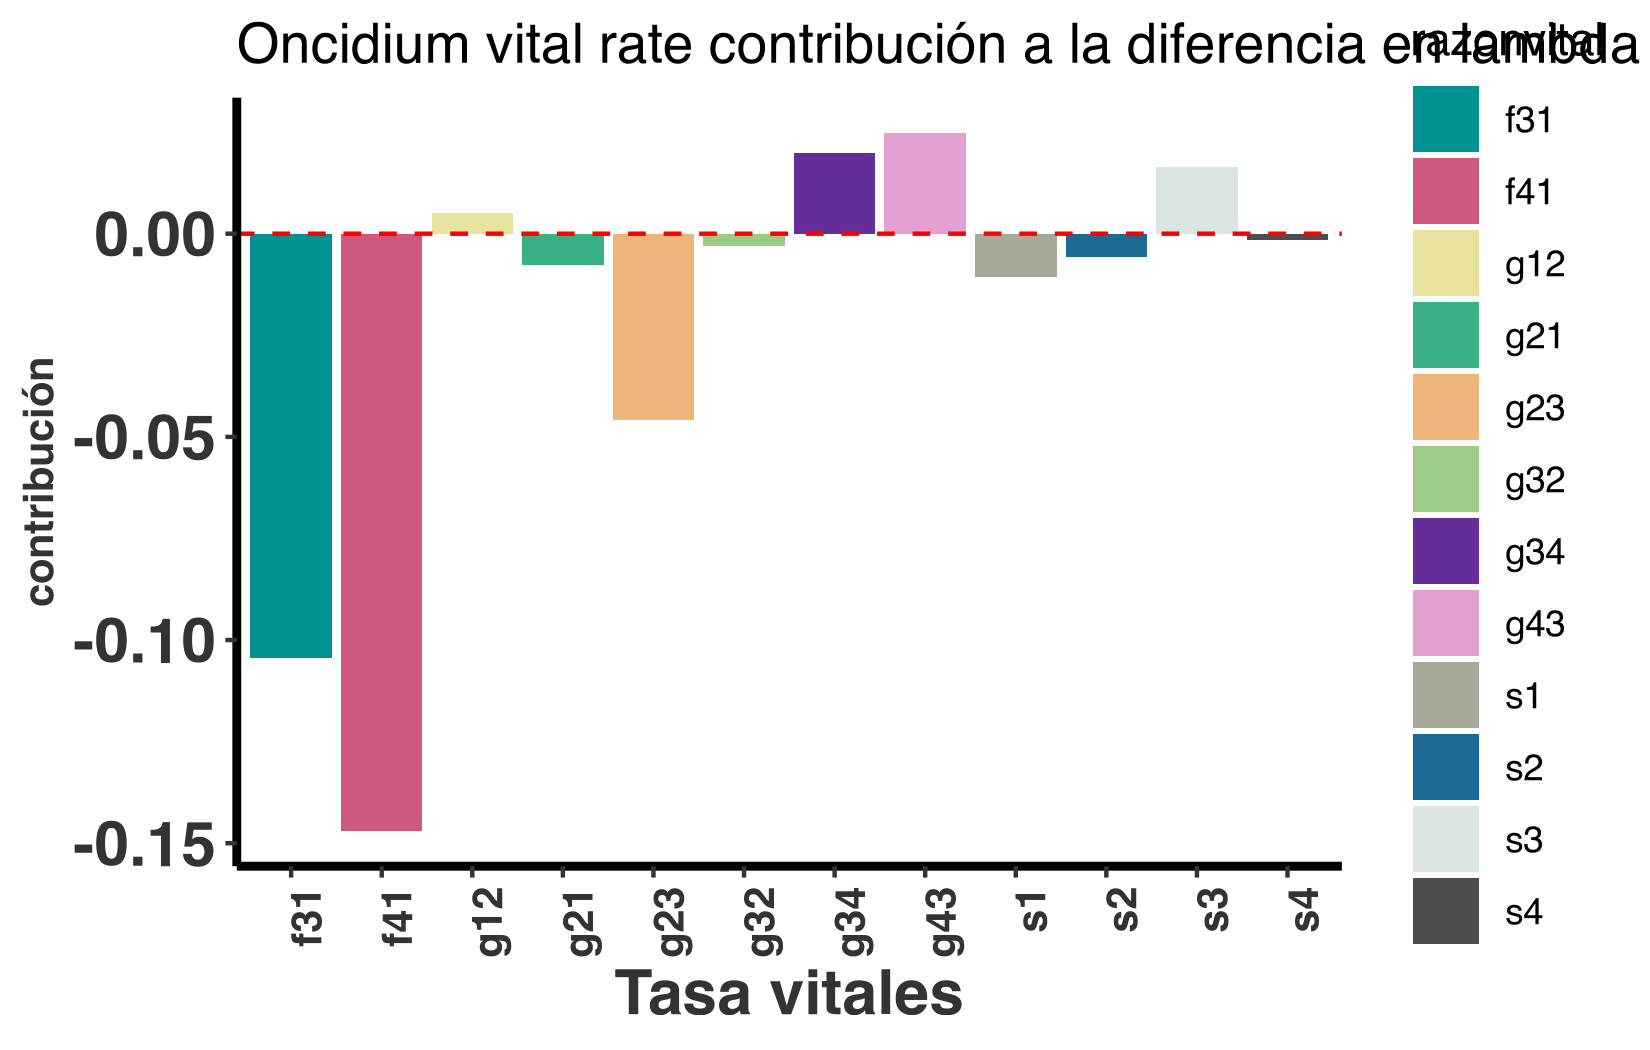
\includegraphics[keepaspectratio]{114-LTRE_files/figure-pdf/LTRE15-1.png}}

Figure 5. Resultados de un Experimento de Respuesta de la Tabla de Vida
(ERTV) llevado a cabo para evaluar las contribuciones de las entradas de
la matriz a la variación observada en \emph{λ}.

\begin{tcolorbox}[enhanced jigsaw, arc=.35mm, bottomrule=.15mm, bottomtitle=1mm, breakable, colback=white, colbacktitle=quarto-callout-tip-color!10!white, colframe=quarto-callout-tip-color-frame, coltitle=black, left=2mm, leftrule=.75mm, opacityback=0, opacitybacktitle=0.6, rightrule=.15mm, title=\textcolor{quarto-callout-tip-color}{\faLightbulb}\hspace{0.5em}{Recomendación}, titlerule=0mm, toprule=.15mm, toptitle=1mm]

\textbf{Lectura del gráfico de contribuciones.}

\begin{itemize}
\tightlist
\item
  \textbf{Barras positivas:} la diferencia observada en esa entrada
  \textbf{incrementa} \(\lambda\) en la condición \(i\) relativa a la
  referencia.
\item
  \textbf{Barras negativas:} la diferencia observada \textbf{reduce}
  \(\lambda\).
\item
  \textbf{Magnitud de la barra:} producto de (i) cuánto cambió la
  entrada y (ii) cuán sensible es \(\lambda\) a esa entrada en la matriz
  promedio.
\end{itemize}

Una contribución pequeña no significa ``esta tasa vital no importa
biológicamente'' --- sólo significa que su variación entre las
condiciones comparadas no movió mucho a \(\lambda\). Para evaluar
importancia biológica intrínseca, conviene complementar con elasticidad.

\end{tcolorbox}

De acuerdo con el análisis de elasticidad para cada una de las
poblaciones de \emph{O. brachyandrum}, tanto en \emph{Q. martinezii}
como en \emph{Q. rugosa} la permanencia de individuos infantiles es la
que tiene un mayor impacto sobre los valores de la tasa de crecimiento
poblacional (Figura 6). De acuerdo al ERTV, el cual toma en cuenta las
diferencias en las tasas vitales y la sensibilidad de lambda que es una
función no linear de esas tasas vitales, podemos observar que la
fecundidad (\(f_{sa}\)) y el crecimiento de plántulas a juveniles
(\(g_{sj}\)), de juveniles a adultos (\(g_{ja}\)) y el retroceso de
adultos a juveniles (\(g_{aj}\)) tiene las mayores contribuciones a las
diferencias en lambda entre \emph{Q. martinezii} y \emph{Q. rugosa} que
la permanencia de plántulas.

Figure 6. Resultados de los análisis de elasticidad, para dos
poblaciones de \emph{Oncidium brachyandrum} creciendo sobre
\emph{Quercus martinezii} y \emph{Q. rugosa}. Por proceso demográfico
(a) y por estadío (b).

\begin{Shaded}
\begin{Highlighting}[]
\FunctionTok{ggplot}\NormalTok{(}
\NormalTok{  LTRE.resultados.Martinezzi.Rugosa,}
  \FunctionTok{aes}\NormalTok{(}\AttributeTok{y =}\NormalTok{ media.sens, }\AttributeTok{x =}\NormalTok{ razonvital, }\AttributeTok{fill =}\NormalTok{ razonvital)}
\NormalTok{) }\SpecialCharTok{+}
  \FunctionTok{geom\_bar}\NormalTok{(}\AttributeTok{stat =} \StringTok{"identity"}\NormalTok{) }\SpecialCharTok{+}
  \FunctionTok{rlt\_style\_fill}\NormalTok{() }\SpecialCharTok{+}
  \FunctionTok{theme}\NormalTok{(}\AttributeTok{axis.text.x =} \FunctionTok{element\_text}\NormalTok{(}\AttributeTok{angle =} \DecValTok{90}\NormalTok{, }\AttributeTok{hjust =} \DecValTok{1}\NormalTok{)) }\SpecialCharTok{+}
  \FunctionTok{labs}\NormalTok{(}
    \AttributeTok{title =} \StringTok{"Promedio de la Sensitividad"}\NormalTok{,}
    \AttributeTok{x =} \StringTok{"razonvital"}\NormalTok{,}
    \AttributeTok{y =} \StringTok{"contribución"}
\NormalTok{  ) }\SpecialCharTok{+}
  \FunctionTok{geom\_hline}\NormalTok{(}\AttributeTok{yintercept =} \DecValTok{0}\NormalTok{, }\AttributeTok{linetype =} \StringTok{"dashed"}\NormalTok{, }\AttributeTok{color =} \StringTok{"red"}\NormalTok{) }\SpecialCharTok{+}
  \FunctionTok{xlab}\NormalTok{(}\StringTok{"Tasa vitales"}\NormalTok{)}
\end{Highlighting}
\end{Shaded}

\pandocbounded{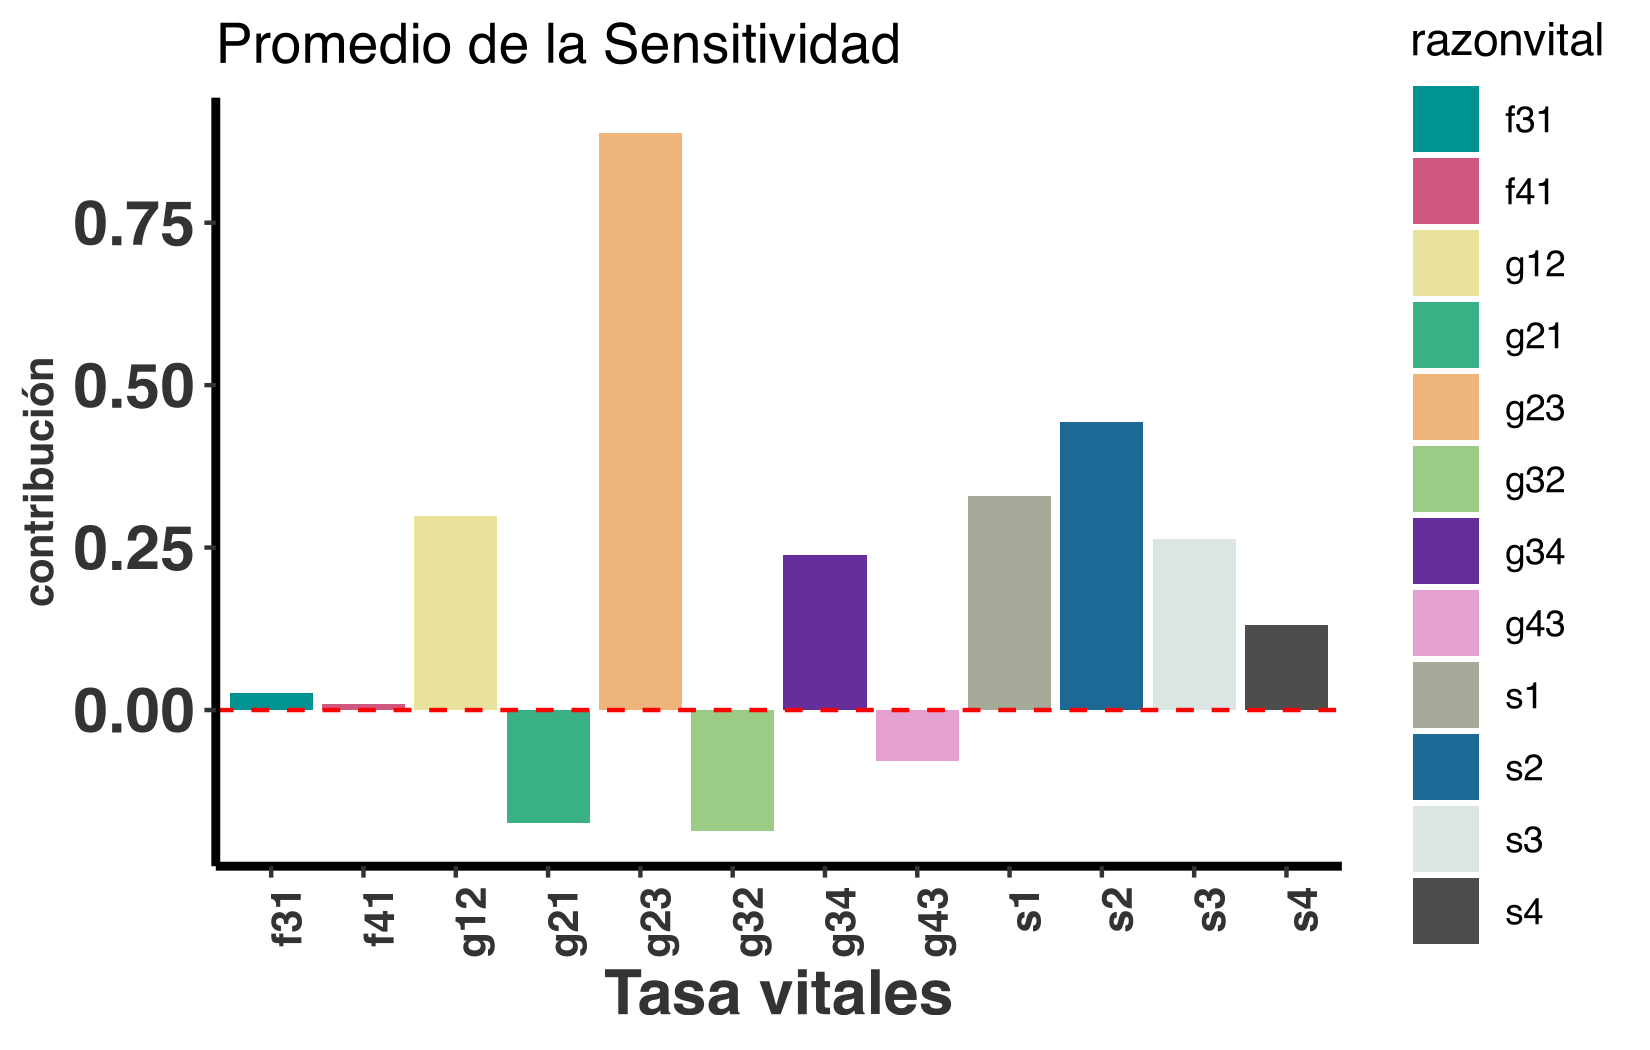
\includegraphics[keepaspectratio]{114-LTRE_files/figure-pdf/LTRE16-1.png}}

\begin{center}\rule{0.5\linewidth}{0.5pt}\end{center}

\section{Análisis con R}\label{anuxe1lisis-con-r}

Ahora enseñar como hacer estos análisis sin tener que usar Excel, aquí
un set de script para aplicar a \emph{Oncidium brachyandrum}.

\begin{center}\rule{0.5\linewidth}{0.5pt}\end{center}

En esta sección se muestra cómo hacer los análisis de ERTV sin tener que
usar Excel, utilizando directamente R. Esto es útil para evitar los
pasos intermedios y realizar el análisis de manera más eficiente.

Calcular la matriz promedio

\begin{Shaded}
\begin{Highlighting}[]
\NormalTok{mat.promedio }\OtherTok{\textless{}{-}}\NormalTok{ (matmart }\SpecialCharTok{+}\NormalTok{ matrug) }\SpecialCharTok{/} \DecValTok{2}

\NormalTok{mat.promedio}
\end{Highlighting}
\end{Shaded}

\begin{verbatim}
      [,1]  [,2] [,3]    [,4]
[1,] 0.660 0.040 1.94 8.26725
[2,] 0.245 0.755 0.25 0.00000
[3,] 0.000 0.105 0.50 0.43000
[4,] 0.000 0.000 0.22 0.53000
\end{verbatim}

\section{Convertir las matrices en un
vectores}\label{convertir-las-matrices-en-un-vectores}

\begin{Shaded}
\begin{Highlighting}[]
\NormalTok{mat.promedio.vector }\OtherTok{\textless{}{-}} \FunctionTok{as.vector}\NormalTok{(mat.promedio)}

\NormalTok{mat.promedio.vector}
\end{Highlighting}
\end{Shaded}

\begin{verbatim}
 [1] 0.66000 0.24500 0.00000 0.00000 0.04000 0.75500 0.10500 0.00000 1.94000
[10] 0.25000 0.50000 0.22000 8.26725 0.00000 0.43000 0.53000
\end{verbatim}

\begin{Shaded}
\begin{Highlighting}[]
\NormalTok{mat\_rug.vector }\OtherTok{\textless{}{-}} \FunctionTok{as.vector}\NormalTok{(matrug) }\CommentTok{\# vector para O. rugosa}
\NormalTok{mat\_mart.vector }\OtherTok{\textless{}{-}} \FunctionTok{as.vector}\NormalTok{(matmart) }\CommentTok{\# vector para O. martinezii}
\end{Highlighting}
\end{Shaded}

\begin{Shaded}
\begin{Highlighting}[]
\NormalTok{mat\_rug.vector}
\end{Highlighting}
\end{Shaded}

\begin{verbatim}
 [1] 0.6400 0.2700 0.0000 0.0000 0.0600 0.7500 0.0800 0.0000 0.0000 0.2700
[11] 0.4700 0.2700 0.0045 0.0000 0.2800 0.6800
\end{verbatim}

\begin{Shaded}
\begin{Highlighting}[]
\NormalTok{matrug}
\end{Highlighting}
\end{Shaded}

\begin{verbatim}
     [,1] [,2] [,3]   [,4]
[1,] 0.64 0.06 0.00 0.0045
[2,] 0.27 0.75 0.27 0.0000
[3,] 0.00 0.08 0.47 0.2800
[4,] 0.00 0.00 0.27 0.6800
\end{verbatim}

Unir los vectores de las matrices \emph{O. rugosa} y \emph{O.
martinezii}

\begin{Shaded}
\begin{Highlighting}[]
\NormalTok{Unido }\OtherTok{=} \FunctionTok{rbind}\NormalTok{(mat\_rug.vector, mat\_mart.vector)}

\NormalTok{Unido}
\end{Highlighting}
\end{Shaded}

\begin{verbatim}
                [,1] [,2] [,3] [,4] [,5] [,6] [,7] [,8] [,9] [,10] [,11] [,12]
mat_rug.vector  0.64 0.27    0    0 0.06 0.75 0.08    0 0.00  0.27  0.47  0.27
mat_mart.vector 0.68 0.22    0    0 0.02 0.76 0.13    0 3.88  0.23  0.53  0.17
                  [,13] [,14] [,15] [,16]
mat_rug.vector   0.0045     0  0.28  0.68
mat_mart.vector 16.5300     0  0.58  0.38
\end{verbatim}

Añadir los nombres a las columnas de la matriz promedio

\begin{Shaded}
\begin{Highlighting}[]
\FunctionTok{colnames}\NormalTok{(Unido)}\OtherTok{\textless{}{-}}\FunctionTok{expression}\NormalTok{(a11, a12, a13, a14, }\CommentTok{\# nota que el orden es por columnas no filas}
\NormalTok{                            a21, a22, a23, a24, }
\NormalTok{                            a31, a32, a33, a34,}
\NormalTok{                            a41, a42, a34, a44)}

\NormalTok{Unido }\OtherTok{=} \FunctionTok{as.data.frame}\NormalTok{(Unido)}
\NormalTok{Unido}\SpecialCharTok{$}\NormalTok{Site }\OtherTok{\textless{}{-}} \FunctionTok{c}\NormalTok{(}\StringTok{"Q. rugosa"}\NormalTok{, }\StringTok{"Q. martinezii"}\NormalTok{)}

\NormalTok{Unido}
\end{Highlighting}
\end{Shaded}

\begin{verbatim}
                 a11  a12 a13 a14  a21  a22  a23 a24  a31  a32  a33  a34
mat_rug.vector  0.64 0.27   0   0 0.06 0.75 0.08   0 0.00 0.27 0.47 0.27
mat_mart.vector 0.68 0.22   0   0 0.02 0.76 0.13   0 3.88 0.23 0.53 0.17
                    a41 a42  a34  a44          Site
mat_rug.vector   0.0045   0 0.28 0.68     Q. rugosa
mat_mart.vector 16.5300   0 0.58 0.38 Q. martinezii
\end{verbatim}

Extraer los elementos del data frame y convertirlos en una lista de
matrices

\begin{Shaded}
\begin{Highlighting}[]
\NormalTok{Ob\_Atrt }\OtherTok{\textless{}{-}} \FunctionTok{lapply}\NormalTok{(}
  \FunctionTok{split}\NormalTok{(}\FunctionTok{as.matrix}\NormalTok{(Unido[, }\DecValTok{1}\SpecialCharTok{:}\DecValTok{16}\NormalTok{]), }\DecValTok{1}\SpecialCharTok{:}\DecValTok{2}\NormalTok{),}
\NormalTok{  matrix,}
  \AttributeTok{ncol =} \DecValTok{4}\NormalTok{,}
  \AttributeTok{byrow =} \ConstantTok{FALSE}
\NormalTok{)}

\FunctionTok{names}\NormalTok{(Ob\_Atrt) }\OtherTok{\textless{}{-}}\NormalTok{ Unido}\SpecialCharTok{$}\NormalTok{Site}

\NormalTok{Ob\_Atrt}
\end{Highlighting}
\end{Shaded}

\begin{verbatim}
$`Q. rugosa`
     [,1] [,2] [,3]   [,4]
[1,] 0.64 0.06 0.00 0.0045
[2,] 0.27 0.75 0.27 0.0000
[3,] 0.00 0.08 0.47 0.2800
[4,] 0.00 0.00 0.27 0.6800

$`Q. martinezii`
     [,1] [,2] [,3]  [,4]
[1,] 0.68 0.02 3.88 16.53
[2,] 0.22 0.76 0.23  0.00
[3,] 0.00 0.13 0.53  0.58
[4,] 0.00 0.00 0.17  0.38
\end{verbatim}

\section{\texorpdfstring{Análisis de ERTV para \emph{Oncidium
brachyandrum}}{Análisis de ERTV para Oncidium brachyandrum}}\label{anuxe1lisis-de-ertv-para-oncidium-brachyandrum}

Gráfico de contribución de ERTV para la matriz promedio de
\emph{Oncidium brachyandrum} creciendo sobre \emph{Quercus martinezii} y
\emph{Q. rugosa}.

\begin{Shaded}
\begin{Highlighting}[]
\NormalTok{Ob }\OtherTok{\textless{}{-}} \FunctionTok{LTRE}\NormalTok{(Ob\_Atrt, mat.promedio)}
\NormalTok{Ob}
\end{Highlighting}
\end{Shaded}

\begin{verbatim}
$`Q. rugosa`
             [,1]         [,2]         [,3]        [,4]
[1,] -0.004507693  0.003547226 -0.066416155 -0.13203195
[2,]  0.010501362 -0.001652761  0.001276096  0.00000000
[3,]  0.000000000 -0.031320325 -0.007254719 -0.01693063
[4,]  0.000000000  0.000000000  0.021664700  0.03033586

$`Q. martinezii`
             [,1]         [,2]         [,3]         [,4]
[1,]  0.005224749 -0.002669011  0.049028094  0.050703995
[2,] -0.016519276  0.001687741 -0.001278465  0.000000000
[3,]  0.000000000  0.035099431  0.007976352  0.009683862
[4,]  0.000000000  0.000000000 -0.027868190 -0.020300386
\end{verbatim}

\section{\texorpdfstring{Analisis de ERTV para \emph{Oncidium
brachyandrum} por
hospedero}{Analisis de ERTV para Oncidium brachyandrum por hospedero}}\label{analisis-de-ertv-para-oncidium-brachyandrum-por-hospedero}

Convertir los resultados de ERTV en un data frame para facilitar la
visualización y manipulación de los datos para usar con ggplot2

\begin{Shaded}
\begin{Highlighting}[]
\NormalTok{Ob }\OtherTok{\textless{}{-}} \FunctionTok{LTRE}\NormalTok{(Ob\_Atrt, mat.promedio) }\CommentTok{\# Realizar el análisis de ERTV usando la matriz promedio}

\NormalTok{Ob\_df\_mart }\OtherTok{\textless{}{-}} \FunctionTok{as.data.frame}\NormalTok{(}\FunctionTok{t}\NormalTok{(Ob}\SpecialCharTok{$}\StringTok{\textasciigrave{}}\AttributeTok{Q. martinezii}\StringTok{\textasciigrave{}}\NormalTok{)) }\CommentTok{\# Convertir los resultados de *Q. martinezii* en un data frame}
\NormalTok{Ob\_df\_rug }\OtherTok{\textless{}{-}} \FunctionTok{as.data.frame}\NormalTok{(}\FunctionTok{t}\NormalTok{(Ob}\SpecialCharTok{$}\StringTok{\textasciigrave{}}\AttributeTok{Q. rugosa}\StringTok{\textasciigrave{}}\NormalTok{)) }\CommentTok{\# Convertir los resultados de *Q. rugosa* en un data frame}

\NormalTok{Ob\_df }\OtherTok{\textless{}{-}} \FunctionTok{rbind}\NormalTok{(Ob\_df\_mart, Ob\_df\_rug)}

\NormalTok{Ob\_df}\SpecialCharTok{$}\NormalTok{Species }\OtherTok{\textless{}{-}} \FunctionTok{c}\NormalTok{( }\CommentTok{\# Asignar nombres de especies, una asignación de nombre por cada fila}
  \StringTok{"Q. martinezii"}\NormalTok{,}
  \StringTok{"Q. martinezii"}\NormalTok{,}
  \StringTok{"Q. martinezii"}\NormalTok{,}
  \StringTok{"Q. martinezii"}\NormalTok{,}
  \StringTok{"Q. rugosa"}\NormalTok{,}
  \StringTok{"Q. rugosa"}\NormalTok{,}
  \StringTok{"Q. rugosa"}\NormalTok{,}
  \StringTok{"Q. rugosa"}
\NormalTok{)}

\FunctionTok{colnames}\NormalTok{(Ob\_df) }\OtherTok{\textless{}{-}} \FunctionTok{c}\NormalTok{(}\StringTok{"a1i"}\NormalTok{, }\StringTok{"a2i"}\NormalTok{, }\StringTok{"a3i"}\NormalTok{, }\StringTok{"a4i"}\NormalTok{, }\StringTok{"Species"}\NormalTok{) }\CommentTok{\# Asignar nombres a las columnas}
\NormalTok{Ob\_df}\SpecialCharTok{$}\NormalTok{t\_1 }\OtherTok{\textless{}{-}} \FunctionTok{c}\NormalTok{(}\StringTok{"ai1"}\NormalTok{, }\StringTok{"ai2"}\NormalTok{, }\StringTok{"ai3"}\NormalTok{, }\StringTok{"ai4"}\NormalTok{, }\StringTok{"ai1"}\NormalTok{, }\StringTok{"ai2"}\NormalTok{, }\StringTok{"ai3"}\NormalTok{, }\StringTok{"ai4"}\NormalTok{) }\CommentTok{\# Asignar nombres a las filas}

\NormalTok{pivot\_long }\OtherTok{\textless{}{-}}\NormalTok{ tidyr}\SpecialCharTok{::}\FunctionTok{pivot\_longer}\NormalTok{( }\CommentTok{\# Convertir a formato largo para ggplot2}
\NormalTok{  Ob\_df, }\CommentTok{\# datos de entrada}
  \AttributeTok{cols =} \FunctionTok{c}\NormalTok{(}\StringTok{"a1i"}\NormalTok{, }\StringTok{"a2i"}\NormalTok{, }\StringTok{"a3i"}\NormalTok{, }\StringTok{"a4i"}\NormalTok{), }\CommentTok{\# columnas a pivotar}
  \AttributeTok{names\_to =} \StringTok{"Transition"}\NormalTok{, }\CommentTok{\# nombre de la nueva columna para las variables}
  \AttributeTok{values\_to =} \StringTok{"Contribution"} \CommentTok{\# nombre de la nueva columna para los valores}
\NormalTok{)}
\NormalTok{pivot\_long}\SpecialCharTok{$}\NormalTok{Transitions2 }\OtherTok{\textless{}{-}} \FunctionTok{c}\NormalTok{(}\StringTok{"a11"}\NormalTok{, }\StringTok{"a12"}\NormalTok{, }\StringTok{"a13"}\NormalTok{, }\StringTok{"a14"}\NormalTok{,  }\CommentTok{\# Asignar nombres a las transiciones}
                             \StringTok{"a21"}\NormalTok{, }\StringTok{"a22"}\NormalTok{, }\StringTok{"a23"}\NormalTok{, }\StringTok{"a24"}\NormalTok{,}
                             \StringTok{"a31"}\NormalTok{, }\StringTok{"a32"}\NormalTok{, }\StringTok{"a33"}\NormalTok{, }\StringTok{"a34"}\NormalTok{, }
                             \StringTok{"a41"}\NormalTok{, }\StringTok{"a42"}\NormalTok{, }\StringTok{"a43"}\NormalTok{, }\StringTok{"a44"}\NormalTok{,}
                             \StringTok{"a11"}\NormalTok{, }\StringTok{"a12"}\NormalTok{, }\StringTok{"a13"}\NormalTok{, }\StringTok{"a14"}\NormalTok{, }
                             \StringTok{"a21"}\NormalTok{, }\StringTok{"a22"}\NormalTok{, }\StringTok{"a23"}\NormalTok{, }\StringTok{"a24"}\NormalTok{,}
                             \StringTok{"a31"}\NormalTok{, }\StringTok{"a32"}\NormalTok{, }\StringTok{"a33"}\NormalTok{, }\StringTok{"a34"}\NormalTok{, }
                             \StringTok{"a41"}\NormalTok{, }\StringTok{"a42"}\NormalTok{, }\StringTok{"a43"}\NormalTok{, }\StringTok{"a44"}\NormalTok{)}

\CommentTok{\# head(pivot\_long)}
\end{Highlighting}
\end{Shaded}

Creación de unos gráficos para ver la contribución de las tasas vitales
sobre la variación en \emph{λ} para cada una de las especies de
hospedero.

\begin{Shaded}
\begin{Highlighting}[]
\FunctionTok{library}\NormalTok{(ggplot2)}

\FunctionTok{ggplot}\NormalTok{(pivot\_long, }\FunctionTok{aes}\NormalTok{(}\AttributeTok{x =}\NormalTok{ Transitions2, }\AttributeTok{y =}\NormalTok{ Contribution, }\AttributeTok{fill =}\NormalTok{ Species)) }\SpecialCharTok{+}
  \FunctionTok{geom\_bar}\NormalTok{(}\AttributeTok{stat =} \StringTok{"identity"}\NormalTok{, }\AttributeTok{position =} \StringTok{"dodge"}\NormalTok{) }\SpecialCharTok{+}
  \FunctionTok{labs}\NormalTok{(}
    \AttributeTok{title =} \StringTok{"Contribución de la variación en las transiciones sobre lambda"}\NormalTok{,}
    \AttributeTok{x =} \StringTok{"Transiciones"}\NormalTok{,}
    \AttributeTok{y =} \StringTok{"Contribuciones a λ"}
\NormalTok{  ) }\SpecialCharTok{+}
 \FunctionTok{rlt\_style\_fill}\NormalTok{()}\SpecialCharTok{+}
 \CommentTok{\# facet\_wrap(\textasciitilde{}Species) +}
  \FunctionTok{theme}\NormalTok{(}\AttributeTok{axis.text.x =} \FunctionTok{element\_text}\NormalTok{(}\AttributeTok{angle =} \DecValTok{45}\NormalTok{, }\AttributeTok{hjust =} \DecValTok{1}\NormalTok{)) }\SpecialCharTok{+}
  \FunctionTok{geom\_hline}\NormalTok{(}\AttributeTok{yintercept =} \DecValTok{0}\NormalTok{, }\AttributeTok{linetype =} \StringTok{"dashed"}\NormalTok{, }\AttributeTok{color =} \StringTok{"red"}\NormalTok{) }\SpecialCharTok{+}
  \FunctionTok{theme}\NormalTok{(}\AttributeTok{legend.position =} \StringTok{"none"}\NormalTok{)}
\end{Highlighting}
\end{Shaded}

\pandocbounded{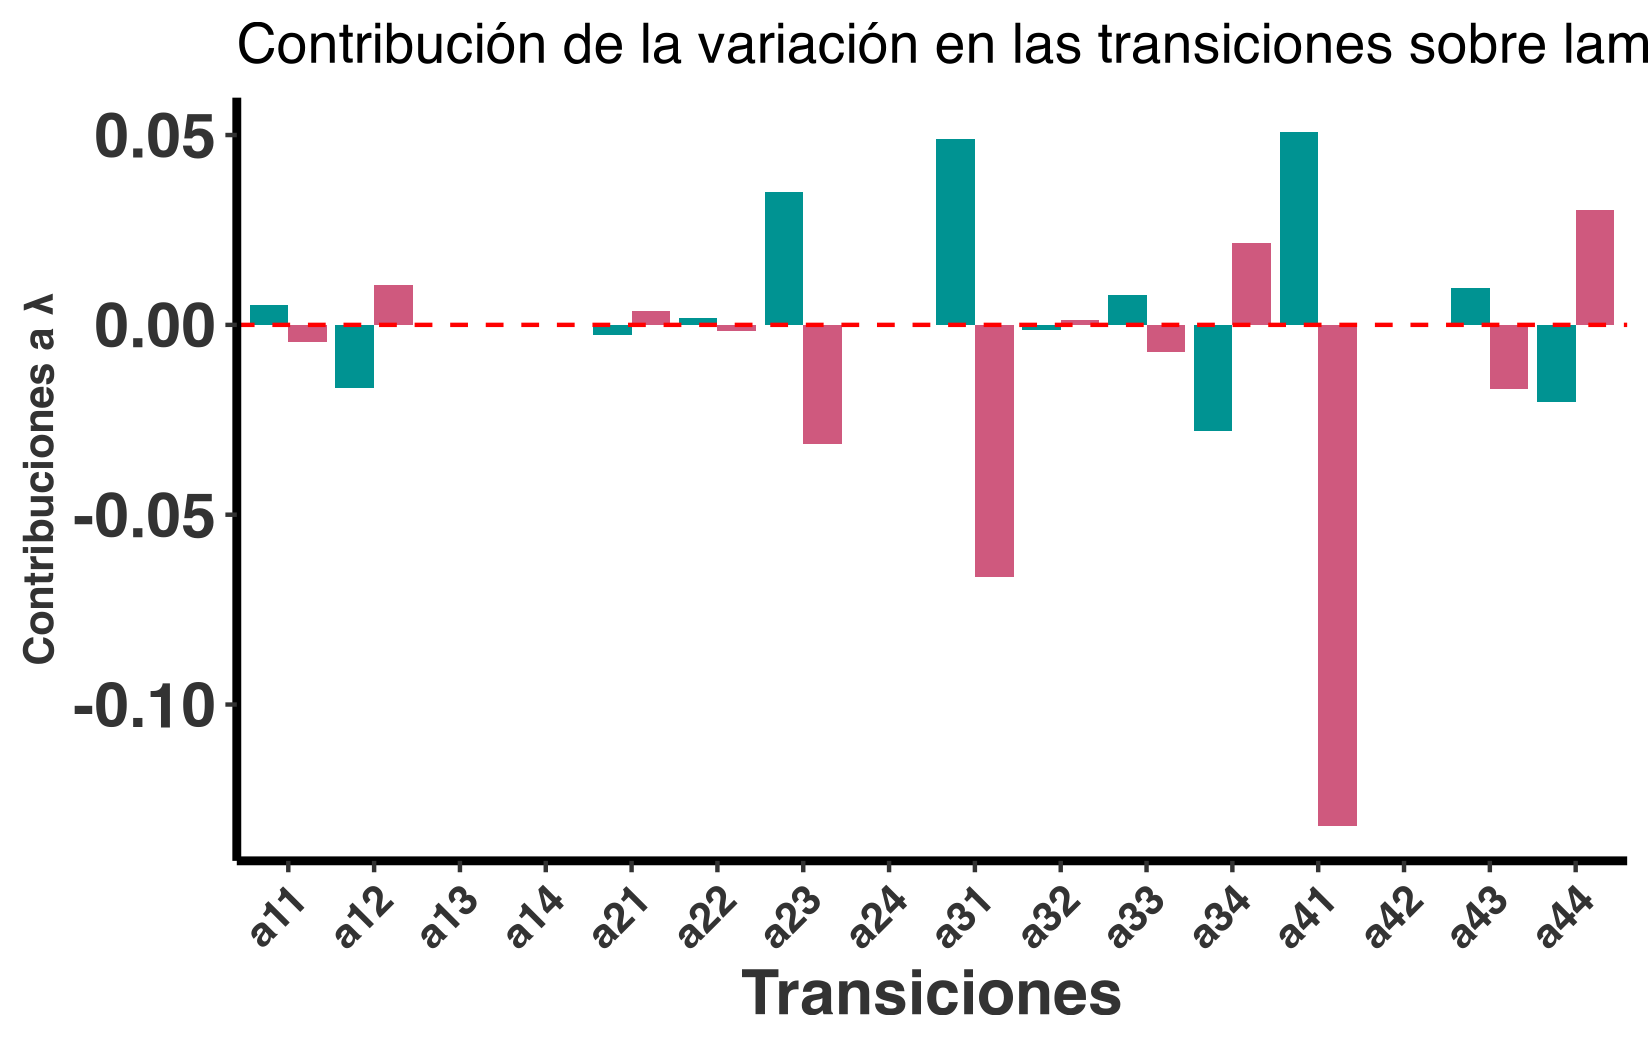
\includegraphics[keepaspectratio]{114-LTRE_files/figure-pdf/LRE25-1.png}}

\section{Alternativa de grafico}\label{alternativa-de-grafico}

\begin{Shaded}
\begin{Highlighting}[]
\FunctionTok{ggplot}\NormalTok{(pivot\_long, }\FunctionTok{aes}\NormalTok{(}\AttributeTok{x =}\NormalTok{ Transitions2, }\AttributeTok{y =}\NormalTok{ Contribution, }\AttributeTok{fill =}\NormalTok{ Species)) }\SpecialCharTok{+}
  \FunctionTok{geom\_bar}\NormalTok{(}\AttributeTok{stat =} \StringTok{"identity"}\NormalTok{, }\AttributeTok{position =} \StringTok{"dodge"}\NormalTok{) }\SpecialCharTok{+}
  \FunctionTok{labs}\NormalTok{(}
    \AttributeTok{title =} \StringTok{"Contribución de la variación en las transiciones sobre lambda"}\NormalTok{,}
    \AttributeTok{x =} \StringTok{"Transiciones"}\NormalTok{,}
    \AttributeTok{y =} \StringTok{"Contribuciones a λ"}
\NormalTok{  ) }\SpecialCharTok{+}
 \FunctionTok{rlt\_style\_fill}\NormalTok{()}\SpecialCharTok{+}
  \FunctionTok{facet\_wrap}\NormalTok{(}\SpecialCharTok{\textasciitilde{}}\NormalTok{Species) }\SpecialCharTok{+}
  \FunctionTok{theme}\NormalTok{(}\AttributeTok{axis.text.x =} \FunctionTok{element\_text}\NormalTok{(}\AttributeTok{angle =} \DecValTok{45}\NormalTok{, }\AttributeTok{hjust =} \DecValTok{1}\NormalTok{)) }\SpecialCharTok{+}
  \FunctionTok{geom\_hline}\NormalTok{(}\AttributeTok{yintercept =} \DecValTok{0}\NormalTok{, }\AttributeTok{linetype =} \StringTok{"dashed"}\NormalTok{, }\AttributeTok{color =} \StringTok{"red"}\NormalTok{) }\SpecialCharTok{+}
  \FunctionTok{theme}\NormalTok{(}\AttributeTok{legend.position =} \StringTok{"none"}\NormalTok{)}
\end{Highlighting}
\end{Shaded}

\pandocbounded{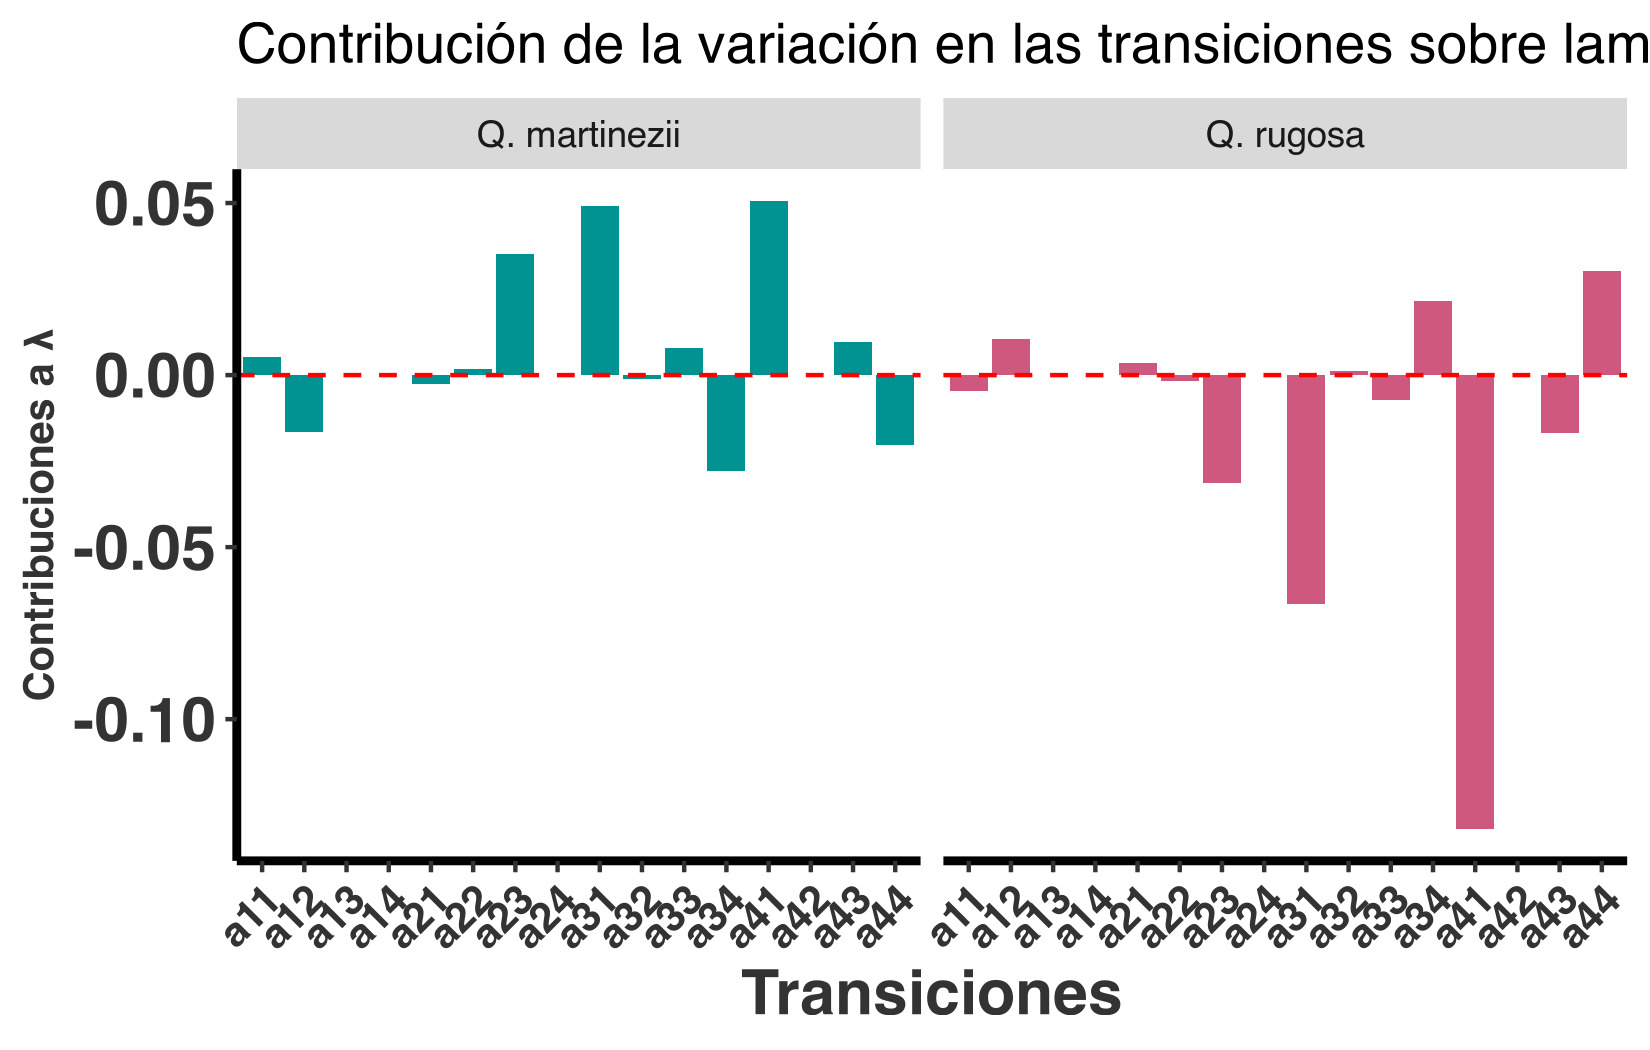
\includegraphics[keepaspectratio]{114-LTRE_files/figure-pdf/LRE26-1.png}}

Aquí se observa el efecto de las transiciones de las tasas vitales sobre
la variación en \emph{λ} para las dos especies de hospedero. Las barras
positivas indican contribuciones positivas a la variación en
\(\lambda\), mientras que las barras negativas indican contribuciones
negativas sobre \(\lambda\). El efecto de las transiciones de las tasas
vitales sobre la variación en \emph{λ} es diferente para cada especie de
hospedero, no solamente el efecto sobre las tasa vitales son diferentes
pero entre hospedero pero los cambios relativos. Lo que indica que las
dinámicas poblacionales de \emph{Oncidium brachyandrum} son
influenciadas por el hospedero en el que crece. Este patrón de cambios
de tasa vitales y su importancia relativa en la variación de \emph{λ}
necesita ser estudiado en más especies de orquídeas epífitas para
entender si es un patrón generalizado o no. Por consecuencia el proximo
paso es evaluar cual son la características de las especies de hospedero
que influyen en la dinámica poblacional de las orquídeas epífitas.

Enlace sobre ERTV https://bookdown.org/cdorm/lefko3gentle/ltre.html

\bookmarksetup{startatroot}

\chapter{Métodos de simulación poblacional}\label{VarTempEsp}

Los métodos de simulación permiten explorar la dinámica poblacional bajo
escenarios variables y condiciones no observadas directamente en los
datos. Este capítulo introduce las simulaciones poblacionales como
herramientas prospectivas para evaluar trayectorias futuras,
variabilidad demográfica y respuestas a cambios en los procesos vitales.

Por: Raymond L. Tremblay

\section{Simulaciones poblacionales y exploración de escenarios
dinámicos}\label{simulaciones-poblacionales-y-exploraciuxf3n-de-escenarios-dinuxe1micos}

Las simulaciones poblacionales constituyen una extensión natural de los
modelos matriciales al permitir proyectar poblaciones bajo condiciones
variables, estocásticas o dependientes del tiempo. A diferencia de los
análisis analíticos que se centran en el comportamiento asintótico, las
simulaciones permiten explorar trayectorias transitorias, evaluar la
variabilidad demográfica y analizar respuestas poblacionales ante
cambios explícitos en los procesos vitales.

En este capítulo se presentan los fundamentos conceptuales de las
simulaciones poblacionales, mostrando cómo pueden implementarse a partir
de matrices de proyección y transiciones demográficas previamente
definidas. Se discuten distintos tipos de simulaciones, incluyendo
simulaciones determinísticas, estocásticas y basadas en escenarios, así
como sus aplicaciones para evaluar extinción, recuperación y efectos de
manejo.

Asimismo, se analiza el papel de las simulaciones como herramientas
complementarias a enfoques analíticos como la elasticidad y los LTRE.
Mientras estos últimos permiten identificar la importancia relativa o
las causas de diferencias observadas, las simulaciones permiten evaluar
\textbf{qué podría ocurrir} bajo condiciones alternativas. Este capítulo
se diferencia de los anteriores porque se enfoca en la exploración
explícita del futuro poblacional, integrando estructura demográfica,
variabilidad y supuestos de manejo para generar predicciones y apoyar la
toma de decisiones en ecología y biología de la conservación.

Las simulaciones se construyen a partir de las transiciones demográficas
introducidas en el capítulo de \hyperref[MatricesT]{Transiciones}. Las
trayectorias simuladas se interpretan en relación con la tasa de
crecimiento poblacional discutida en el capítulo de
\hyperref[Crecimiento_Poblacional]{Crecimiento poblacional}. A
diferencia de los análisis \hyperref[ERTV]{LTRE}, que explican
diferencias observadas, las simulaciones permiten explorar escenarios
futuros no observados. Las simulaciones pueden extenderse naturalmente
dentro de un marco bayesiano, como se describe en el capítulo de
\hyperref[acercamiento-bayesiano-para-calcular-transiciones-y-fecundidades]{Acercamiento
bayesiano}.

\subsubsection{Librerías de R requeridas para el siguiente
módulo}\label{libreruxedas-de-r-requeridas-para-el-siguiente-muxf3dulo-12}

\begin{Shaded}
\begin{Highlighting}[]
\FunctionTok{library}\NormalTok{(tidyverse)}
\FunctionTok{library}\NormalTok{(ggtext)}
\FunctionTok{library}\NormalTok{(janitor)}
\FunctionTok{library}\NormalTok{(popbio)}
\FunctionTok{library}\NormalTok{(raretrans)}
\FunctionTok{library}\NormalTok{(ggpubr)}
\end{Highlighting}
\end{Shaded}

\begin{Shaded}
\begin{Highlighting}[]
\NormalTok{rlt\_theme }\OtherTok{\textless{}{-}} \FunctionTok{theme}\NormalTok{(}
  \AttributeTok{axis.title.y =} \FunctionTok{element\_text}\NormalTok{(}\AttributeTok{colour =} \StringTok{"grey20"}\NormalTok{, }\AttributeTok{size =} \DecValTok{10}\NormalTok{, }\AttributeTok{face =} \StringTok{"bold"}\NormalTok{),}
  \AttributeTok{axis.text.x =} \FunctionTok{element\_text}\NormalTok{(}\AttributeTok{colour =} \StringTok{"grey20"}\NormalTok{, }\AttributeTok{size =} \DecValTok{10}\NormalTok{, }\AttributeTok{face =} \StringTok{"bold"}\NormalTok{),}
  \AttributeTok{axis.text.y =} \FunctionTok{element\_text}\NormalTok{(}\AttributeTok{colour =} \StringTok{"grey20"}\NormalTok{, }\AttributeTok{size =} \DecValTok{15}\NormalTok{, }\AttributeTok{face =} \StringTok{"bold"}\NormalTok{),}
  \AttributeTok{axis.title.x =} \FunctionTok{element\_text}\NormalTok{(}\AttributeTok{colour =} \StringTok{"grey20"}\NormalTok{, }\AttributeTok{size =} \DecValTok{15}\NormalTok{, }\AttributeTok{face =} \StringTok{"bold"}\NormalTok{)}
\NormalTok{) }\SpecialCharTok{+}
  \FunctionTok{theme}\NormalTok{(}
    \CommentTok{\# Remover los bordes}
    \AttributeTok{panel.border =} \FunctionTok{element\_blank}\NormalTok{(),}
    \CommentTok{\# Remover las líneas}
    \AttributeTok{panel.grid.major =} \FunctionTok{element\_blank}\NormalTok{(),}
    \AttributeTok{panel.grid.minor =} \FunctionTok{element\_blank}\NormalTok{(),}
    \CommentTok{\# Remover el fondo del panel}
    \AttributeTok{panel.background =} \FunctionTok{element\_blank}\NormalTok{(),}
    \CommentTok{\# añadir lineas más gruesas}
    \AttributeTok{axis.line.x =} \FunctionTok{element\_line}\NormalTok{(}\AttributeTok{colour =} \StringTok{"black"}\NormalTok{, }\AttributeTok{linewidth =} \DecValTok{1}\NormalTok{),}
    \AttributeTok{axis.line.y =} \FunctionTok{element\_line}\NormalTok{(}\AttributeTok{colour =} \StringTok{"black"}\NormalTok{, }\AttributeTok{linewidth =} \DecValTok{1}\NormalTok{)}
\NormalTok{  )}

\NormalTok{diverging}\OtherTok{=} \FunctionTok{c}\NormalTok{(}\StringTok{"\#009392"}\NormalTok{,}\StringTok{"\#CF597E"}\NormalTok{,}\StringTok{"\#E9E29C"}\NormalTok{, }\StringTok{"\#39B185"}\NormalTok{,}\StringTok{"\#EEB479"}\NormalTok{ , }\StringTok{"\#9CCB86"}\NormalTok{ )}

\CommentTok{\# {-}{-}{-} 2. Combinarlos en un objeto de tipo lista {-}{-}{-}}
\CommentTok{\# Esta lista se puede añadir al gráfico con un solo \textquotesingle{}+\textquotesingle{}}
\NormalTok{rlt\_style\_fill }\OtherTok{\textless{}{-}} \ControlFlowTok{function}\NormalTok{() \{}
  \FunctionTok{list}\NormalTok{(}
\NormalTok{    rlt\_theme,}
    \FunctionTok{scale\_fill\_manual}\NormalTok{(}\AttributeTok{values =}\NormalTok{ diverging)}
\NormalTok{  )}
\NormalTok{\}}

\NormalTok{rlt\_style\_colour }\OtherTok{\textless{}{-}} \ControlFlowTok{function}\NormalTok{() \{}
  \FunctionTok{list}\NormalTok{(}
\NormalTok{    rlt\_theme,}
    \FunctionTok{scale\_colour\_manual}\NormalTok{(}\AttributeTok{values =}\NormalTok{ diverging)}
\NormalTok{  )}
\NormalTok{\}}
\end{Highlighting}
\end{Shaded}

\section{Implementación de simulaciones
poblacionales}\label{implementaciuxf3n-de-simulaciones-poblacionales}

A continuación se describen los procedimientos para implementar
simulaciones poblacionales a partir de matrices de proyección y
transiciones demográficas, incluyendo ejemplos determinísticos y
estocásticos.

El término \textbf{biología} pudiese ser un sinónimo de variación
biológica. No hay dos organismos iguales, ni siquiera gemelos/clones que
sean completamente idénticos. La variación biológica es una
característica fundamental de la vida y es la base de la evolución; no
puede haber evolución sin variación. Cuando consideramos los individuos,
por ejemplo humanos, fácilmente reconocemos variación ---en tamaño,
color de ojos, susceptibilidad a cáncer o infección, y efecto del
ambiente (por ejemplo la dieta o acceso a la educación)--- entre muchos
factores que impactan la supervivencia, crecimiento y reproducción. Pero
desafortunadamente cuando consideramos los animales y plantas de una
misma especie, frecuentemente se obvia la variación en los análisis.
Podemos observar variación a múltiples niveles en una misma especie:

\begin{itemize}
\tightlist
\item
  Variación sub-individual (dentro de un individuo), un concepto bien
  desarrollado por Carlos Herrera de la Universidad de Sevilla (Herrera,
  2009). Esta variación nunca ha sido incluida en modelos MPP.
\item
  Variación entre individuos (dentro de una población).
\item
  Variación entre poblaciones.
\item
  Variación temporal (entre periodos de tiempo).
\end{itemize}

Todos estos componentes de variación tendrán impacto en la dispersión de
los estimados de los parámetros de la matriz de transición y el
crecimiento poblacional, además del comportamiento de la población en el
tiempo. Hay un componente que frecuentemente se deja en el olvido: el
efecto de la variación por \textbf{tamaño de muestra pequeño} sobre los
estimados, que llamamos \textbf{estocasticidad demográfica}. En este
capítulo se discute el efecto de la variación en tiempo, espacio y
tamaño de muestra sobre los estimados de los parámetros de la matriz y
el crecimiento poblacional.

\subsection{Componentes de Variación}\label{componentes-de-variaciuxf3n}

\subsubsection{La variación
sub-individual}\label{la-variaciuxf3n-sub-individual}

La variación sub-individual es la variación que se observa en un
individuo. Por ejemplo, la variación en el \textbf{tamaño} de hojas,
flores, frutos, semillas dentro del mismo individuo o la
\textbf{cantidad} hojas, flores, frutos, semillas en tiempos distintos.
Este tipo de variación es común en plantas y es un componente importante
de la variación total pero raramente se considera en los análisis.
Carlos Herrera ha demostrado claramente que este componente no solamente
es parte de la variación total de las especies pero es importante para
entender los procesos ecológicos y evolutivos (Herrera, 2009). En
adición cuando uno compara la variación total por la variación
sub-individual, la variación sub-individual es mucho más grande que la
variación entre individuos y poblaciones. Esta variación al conocimiento
de los presentes autores nunca ha sido incluido en análisis de dinámica
poblacional y integrado dentro un MPP. En un estudio del tamaño de las
flores en \emph{Lepanthes rupestris} se observó que la variación en el
tamaño de flores disminuye a largo de la inflorescencia y que la
probabilidad de remoción de pollinia y de deposición de estas sobre el
estigma no siguen el mismo patrón, la probabilidades de remoción de
pollinia aumenta con flores más pequeñas pero la probabilidad de frutos
disminuye (Tremblay, 2006). Por consecuencia, cuando se recolecta la
información sobre el esfuerzo reproductivo de una especie, puede ser que
la variación sub-individual impacta los estimados de la matriz de
transiciones debido que las flores en este periodo eran de diferentes
tamaños. Las inflorescencias de \emph{Lepanthes} pueden ser activas
produciendo flores por meses y años (Tremblay, com. pers.).

\subsubsection{La variación entre
individuos}\label{la-variaciuxf3n-entre-individuos}

La variación entre individuos es la diferencias que se observa entre
individuos de una misma población. Por ejemplo, la variación en el
tamaño de los individuos, cantidad de hojas, cantidad de flores,
cantidad de frutos entre individuos de una misma población influye en la
probabilidad de sobrevivir, crecer y reproducirse. La variación entre
individuos de diferentes tamaños o etapas impacta grandemente la
supervivencia, crecimiento y reproducción de los individuos. Los
trabajos de Harper y otros han demostrado que esa variación es común en
las plantas (Harper, 1977) y típicamente es más importante que la edad
de los individuos en la mayoría de las plantas. En orquídea un ejemplo
de esa variación es que la mayoría de los individuos reproductivos en
una población no produce frutos (Ackerman et~al., 2020).

\subsubsection{La variación entre
poblaciones}\label{la-variaciuxf3n-entre-poblaciones}

La variación entre poblaciones es la variación que se observa entre
grupos de individuos de una misma especie en diferentes sitios.
Poblaciones distintas pudiesen ser influenciadas por las diferencias
abióticas e interacciones bióticas únicas a cada población. Esa
variación pudiese influenciar la dinámica de cada población y la
dinámica de la especie en general. Las diferencias entre poblaciones
pudiesen ser influenciadas por condiciones específicas como la variación
genética entre poblaciones, variación abiótica (recursos como el agua,
nitrógeno, luz), variación en la interacción biótica (e.g.~micorriza,
diversidad y cantidad de polinizadores, tipo de forófitos), variación en
la historia de la población (procesos de sucesión), entre otros
factores, además de la plasticidad fenotípica que se define como la
interacción del ambiente sobre la expresión genética ({Nicotra et~al.},
2010). Sin duda, las variables abióticas y bióticas pueden influenciar
las transiciones, estasis y reproducción de forma diferencial entre las
diferentes etapas del ciclo de vida de la especie.

\subsubsection{La variación entre
tiempo}\label{la-variaciuxf3n-entre-tiempo}

Este componente de variación incluye la variación típicamente
relacionada a la variación \emph{abiótica} que cambia de un periodo de
tiempo a otro; por ejemplo, el efecto de la cantidad de lluvia, número
de días sin lluvia, temperatura, entre muchas otras variables. Pero no
se debería limitar a considerar solamente la variación abiótica en el
tiempo, ya que la variación \emph{biótica} también puede cambiar de un
periodo de tiempo a otro. Por ejemplo, la densidad y/o composición de
especies en una comunidad cambia de un periodo de tiempo a otro, e
incluso la variación de patógenos y otras interacciones bióticas
alrededor de la especie de interés. Todo lo anterior pudiese influenciar
la dinámica y los estimados de los parámetros de la matriz. Por ejemplo,
considera la variación en la presencia de herbívoros o patógenos que
cambia de un periodo de tiempo a otro, resultando en variación en la
competencia interespecífica. Por consecuencia, la variación en el tiempo
es mucho más que la variación \emph{abiótica} en el tiempo. Allí, uno
también tiene que incluir el efecto de bonanzas (eventos raros
positivos, por ejemplo: reclutamiento excepcional en algunos años)
(Antonini, Dirzo \& Cassia Quitete-Portela, 2020) y catástrofes (eventos
raros negativos, por ejemplo: huracanes, mortandad de un hospedero)
(Hiernaux et~al., 2009), que pudiesen influenciar la dinámica de la
especie de interés. Un ejemplo drástico de su impacto es la mortandad
casi completa de epífitas al pasar huracanes fuertes (Goode \& Allen,
2008), o que el efecto sea diferencial entre especies o sustratos
(Rodrı́guez-Robles, Ackerman \& Meléndez, 1990).

\subsubsection{Variación en tamaño de muestra
pequeña}\label{variaciuxf3n-en-tamauxf1o-de-muestra-pequeuxf1a}

La gran mayoría de los estudios usando MPP son para evaluar la
probabilidad de supervivencia en una especie en peligro de extinción. La
razón principal de estos estudios es que quedan muy pocos individuos en
la población o pocas poblaciones, y esas poblaciones se consideran en
riesgo.

Por ejemplo si tuviésemos en una población solamente de un adulto y este
adulto sobrevive de un año a otro entonces la probabilidad de
supervivencia es 1.0. Pero si tuviésemos solamente un adulto y este
adulto muere entonces la probabilidad de supervivencia es 0.0. Las
probabilidad de supervivencia pueden ser solamente 1.0 o 0.0
respectivamente y otros valores no son posibles, pero la interpretación
biológica es sesgada, porque ya hay solamente dos alternativas. Pero si
tuviésemos 1,000 o 10,000 individuos es muy poco probable que todos se
mueren o todos sobreviven, y hay muchas alternativas posibles. Este es
un ejemplo extremo pero ilustra claramente el problema de estimar la
probabilidad de supervivencia y transiciones en una población con un
tamaño de muestra pequeña y puede resultar en estimados sesgados.

En las próximas secciones vemos métodos de simulaciones y estimaciones
de intervalos de confianza para abordar la variación biológica en tiempo
y espacio y la variación por el tamaño de muestra pequeña.

\begin{tcolorbox}[enhanced jigsaw, arc=.35mm, bottomrule=.15mm, bottomtitle=1mm, breakable, colback=white, colbacktitle=quarto-callout-important-color!10!white, colframe=quarto-callout-important-color-frame, coltitle=black, left=2mm, leftrule=.75mm, opacityback=0, opacitybacktitle=0.6, rightrule=.15mm, title=\textcolor{quarto-callout-important-color}{\faExclamation}\hspace{0.5em}{Importante}, titlerule=0mm, toprule=.15mm, toptitle=1mm]

\textbf{Tres fuentes de incertidumbre que las simulaciones pueden
capturar.}

\begin{itemize}
\tightlist
\item
  \textbf{Estocasticidad espacial:} variación entre poblaciones de la
  misma especie. Se modela seleccionando aleatoriamente entre matrices
  de distintos sitios.
\item
  \textbf{Estocasticidad temporal:} variación entre años o periodos. Se
  modela seleccionando aleatoriamente entre matrices de distintos
  tiempos.
\item
  \textbf{Estocasticidad demográfica:} variación intrínseca debida al
  tamaño de muestra pequeño. Se modela usando distribuciones
  beta/Dirichlet sobre los parámetros (enfoque bayesiano).
\end{itemize}

Las tres pueden combinarse en un solo modelo, pero conviene evaluarlas
por separado para entender cuál domina en una población dada.

\end{tcolorbox}

\begin{center}\rule{0.5\linewidth}{0.5pt}\end{center}

\section{Introducción a los métodos de
simulaciones}\label{introducciuxf3n-a-los-muxe9todos-de-simulaciones}

Los métodos de simulaciones para estimar la variación en los parámetros
tanto de la matriz como el crecimiento poblacional varía mucho. Lo que
es consistente es que se utilizan datos disponibles para hacer
simulaciones y estimar la variación en los parámetros. En otras palabras
se usa la variación entre los elementos de múltiples matrices de
transición en tiempo o espacio o el tamaño de muestra para hacer
simulaciones y estimar la dispersión en los parámetros. La manera de
observar la variación puede asumir diferentes formas, por ejemplo, la
variación en los parámetros de la matriz de transición puede ser
expresada como una distribución normal (distribución en forma de
campana), una distribución de Poisson (datos con valores discretos, 0,
1, 2\ldots{} etc.), una distribución binomial (distribución donde hay
solamente dos alternativas) o beta (distribución donde el rango es
limitado a los valores entre 0 y 1, inclusive), entre otras
distribuciones. Reconocer el tipo de variación en los parámetros de la
matriz de transición es importante para escoger el método de
simulaciones y estimaciones de intervalos de confianza y reconocer sus
limitaciones e interpretación.

\section{Estocasticidad espacial}\label{estocasticidad-espacial}

En este caso vemos el efecto de la variación espacial en la probabilidad
en los estimados. Aquí nos interesa descubrir y cuantificar cuan
variable son las poblaciones una del otro. El objetivo es determinar si
las poblaciones se comporta similar una del otro o varía mucho de un
sitio al otro.

\begin{center}\rule{0.5\linewidth}{0.5pt}\end{center}

\subsection{Entrada de datos}\label{entrada-de-datos}

El primer paso es definir la diferentes matriz, una por cada periodo de
tiempo. En el siguiente script se enseña como entrar los datos para
múltiples matrices en un solo objeto. Nota que es una lista de matriz.

\begin{figure}[H]

{\centering \pandocbounded{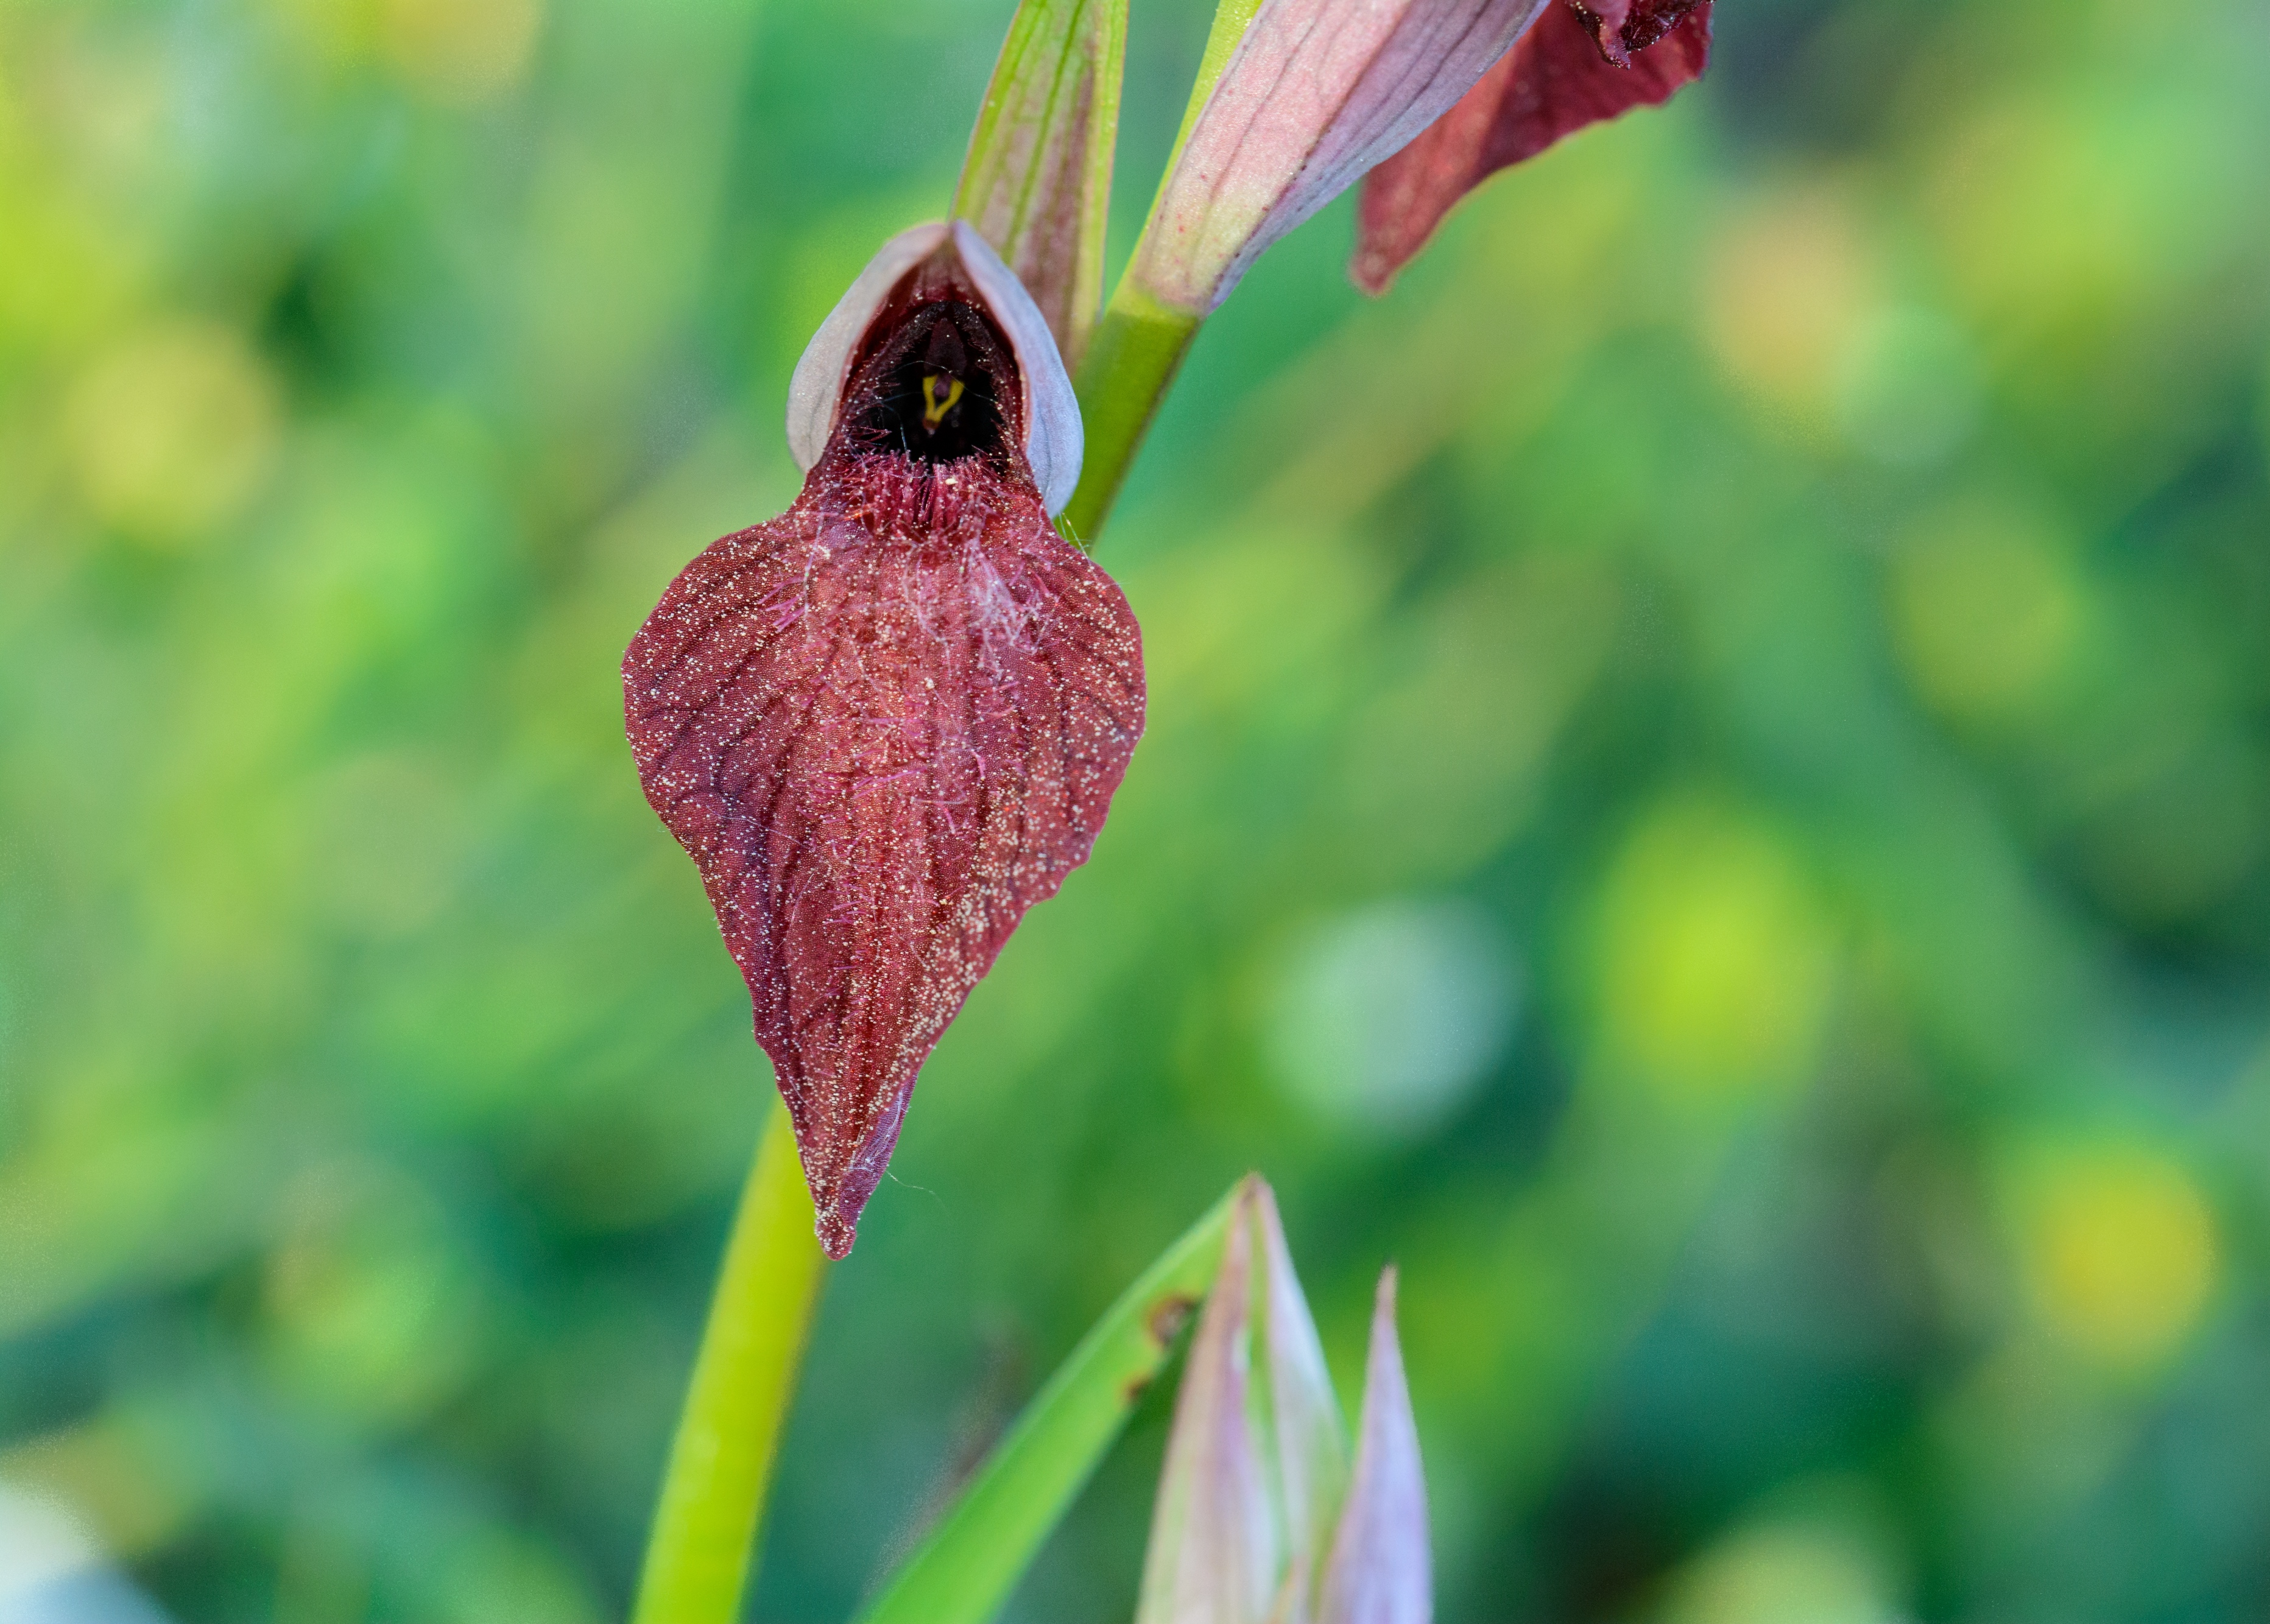
\includegraphics[keepaspectratio]{images/Serapias_cordigera_5_Giuseppe_Pellegrino.jpeg}}

}

\caption{\emph{Serapias cordigera}. Foto: Guiseppe Pelligrino}

\end{figure}%

Los datos provienen de un estudio de la dinámica de una población de
\emph{Serapias cordigera} de 1999 al 2012 evaluando el impacto
antropogénico sobre la dinámica de la población (Pellegrino \& Bellusci,
2014). En este caso se emplea solamente 6 matrices de transición de la
población de \emph{Serapias cordigera} en 1999, tres de estas son
poblaciones que tienen impacto antropogénico (A1, A2 y A3) y tres
poblaciones naturales, sin impacto antropogénico (N1, N2, N3). Nota que
se construye una lista (list()) de matriz de transición, una por cada
periodo de tiempo.

\begin{Shaded}
\begin{Highlighting}[]
\NormalTok{Serapia}\OtherTok{\textless{}{-}}\FunctionTok{list}\NormalTok{(}
  \AttributeTok{A1\_1999=}\FunctionTok{matrix}\NormalTok{(}\FunctionTok{c}\NormalTok{(}
\FloatTok{0.745}\NormalTok{,  }\FloatTok{0.152}\NormalTok{,  }\FloatTok{0.452}\NormalTok{,  }\FloatTok{0.564}\NormalTok{,}
\FloatTok{0.125}\NormalTok{,  }\FloatTok{0.000}\NormalTok{,  }\FloatTok{0.000}\NormalTok{,  }\FloatTok{0.000}\NormalTok{,}
\FloatTok{0.000}\NormalTok{,  }\FloatTok{0.321}\NormalTok{,  }\FloatTok{0.205}\NormalTok{,  }\FloatTok{0.342}\NormalTok{,}
\FloatTok{0.200}\NormalTok{,  }\FloatTok{0.365}\NormalTok{,  }\FloatTok{0.205}\NormalTok{,  }\FloatTok{0.185}
\NormalTok{  ),}
  \AttributeTok{nrow=}\DecValTok{4}\NormalTok{, }\AttributeTok{byrow=}\ConstantTok{TRUE}\NormalTok{,}
  \AttributeTok{dimnames=}\FunctionTok{list}\NormalTok{(}\FunctionTok{c}\NormalTok{(}\StringTok{"latente"}\NormalTok{, }\StringTok{"plantula"}\NormalTok{, }\StringTok{"rosetta"}\NormalTok{, }\StringTok{"con flor"}\NormalTok{),}
                \FunctionTok{c}\NormalTok{(}\StringTok{"latente"}\NormalTok{, }\StringTok{"plantula"}\NormalTok{, }\StringTok{"rosetta"}\NormalTok{, }\StringTok{"con flor"}\NormalTok{)}
\NormalTok{  )}
\NormalTok{  ),}
\AttributeTok{A2\_1999=}\FunctionTok{matrix}\NormalTok{(}\FunctionTok{c}\NormalTok{(}
\FloatTok{0.648}\NormalTok{,  }\FloatTok{0.203}\NormalTok{,  }\FloatTok{0.414}\NormalTok{,  }\FloatTok{0.604}\NormalTok{,}
\FloatTok{0.188}\NormalTok{,  }\FloatTok{0.000}\NormalTok{,  }\FloatTok{0.000}\NormalTok{,  }\FloatTok{0.000}\NormalTok{,}
\FloatTok{0.000}\NormalTok{,  }\FloatTok{0.342}\NormalTok{,  }\FloatTok{0.198}\NormalTok{,  }\FloatTok{0.377}\NormalTok{,}
\FloatTok{0.242}\NormalTok{,  }\FloatTok{0.264}\NormalTok{,  }\FloatTok{0.225}\NormalTok{,  }\FloatTok{0.191}
\NormalTok{),}
 \AttributeTok{nrow=}\DecValTok{4}\NormalTok{, }\AttributeTok{byrow=}\ConstantTok{TRUE}\NormalTok{,}
  \AttributeTok{dimnames=}\FunctionTok{list}\NormalTok{(}\FunctionTok{c}\NormalTok{(}\StringTok{"latente"}\NormalTok{, }\StringTok{"plantula"}\NormalTok{, }\StringTok{"rosetta"}\NormalTok{, }\StringTok{"con flor"}\NormalTok{),}
                \FunctionTok{c}\NormalTok{(}\StringTok{"latente"}\NormalTok{, }\StringTok{"plantula"}\NormalTok{, }\StringTok{"rosetta"}\NormalTok{, }\StringTok{"con flor"}\NormalTok{)}
\NormalTok{  )}
\NormalTok{  ),}
\AttributeTok{A3\_1999=}\FunctionTok{matrix}\NormalTok{(}\FunctionTok{c}\NormalTok{(}
\FloatTok{0.544}\NormalTok{,  }\FloatTok{0.223}\NormalTok{,  }\FloatTok{0.364}\NormalTok{,  }\FloatTok{0.498}\NormalTok{,}
\FloatTok{0.148}\NormalTok{,  }\FloatTok{0.000}\NormalTok{,  }\FloatTok{0.000}\NormalTok{,  }\FloatTok{0.000}\NormalTok{,}
\FloatTok{0.000}\NormalTok{,  }\FloatTok{0.249}\NormalTok{,  }\FloatTok{0.243}\NormalTok{,  }\FloatTok{0.287}\NormalTok{,}
\FloatTok{0.242}\NormalTok{,  }\FloatTok{0.303}\NormalTok{,  }\FloatTok{0.210}\NormalTok{,  }\FloatTok{0.101}
\NormalTok{),}
\AttributeTok{nrow=}\DecValTok{4}\NormalTok{, }\AttributeTok{byrow=}\ConstantTok{TRUE}\NormalTok{,}
  \AttributeTok{dimnames=}\FunctionTok{list}\NormalTok{(}\FunctionTok{c}\NormalTok{(}\StringTok{"latente"}\NormalTok{, }\StringTok{"plantula"}\NormalTok{, }\StringTok{"rosetta"}\NormalTok{, }\StringTok{"con flor"}\NormalTok{),}
                \FunctionTok{c}\NormalTok{(}\StringTok{"latente"}\NormalTok{, }\StringTok{"plantula"}\NormalTok{, }\StringTok{"rosetta"}\NormalTok{, }\StringTok{"con flor"}\NormalTok{)}
\NormalTok{  )}
\NormalTok{  ),}
\AttributeTok{N1\_1999=}\FunctionTok{matrix}\NormalTok{(}\FunctionTok{c}\NormalTok{(}
\FloatTok{0.287}\NormalTok{,  }\FloatTok{0.271}\NormalTok{,  }\FloatTok{0.054}\NormalTok{,  }\FloatTok{0.107}\NormalTok{,}
\FloatTok{0.318}\NormalTok{,  }\FloatTok{0.000}\NormalTok{,  }\FloatTok{0.000}\NormalTok{,  }\FloatTok{0.000}\NormalTok{,}
\FloatTok{0.000}\NormalTok{,  }\FloatTok{0.438}\NormalTok{,  }\FloatTok{0.228}\NormalTok{,  }\FloatTok{0.273}\NormalTok{,}
\FloatTok{0.111}\NormalTok{,  }\FloatTok{0.512}\NormalTok{,  }\FloatTok{0.585}\NormalTok{,  }\FloatTok{0.542}
\NormalTok{),}
\AttributeTok{nrow=}\DecValTok{4}\NormalTok{, }\AttributeTok{byrow=}\ConstantTok{TRUE}\NormalTok{,}
  \AttributeTok{dimnames=}\FunctionTok{list}\NormalTok{(}\FunctionTok{c}\NormalTok{(}\StringTok{"latente"}\NormalTok{, }\StringTok{"plantula"}\NormalTok{, }\StringTok{"rosetta"}\NormalTok{, }\StringTok{"con flor"}\NormalTok{),}
                \FunctionTok{c}\NormalTok{(}\StringTok{"latente"}\NormalTok{, }\StringTok{"plantula"}\NormalTok{, }\StringTok{"rosetta"}\NormalTok{, }\StringTok{"con flor"}\NormalTok{)}
\NormalTok{  )}
\NormalTok{  ),}
\AttributeTok{N2\_1999=}\FunctionTok{matrix}\NormalTok{(}\FunctionTok{c}\NormalTok{(}
\FloatTok{0.299}\NormalTok{,  }\FloatTok{0.253}\NormalTok{,  }\FloatTok{0.066}\NormalTok{,  }\FloatTok{0.182}\NormalTok{,}
\FloatTok{0.324}\NormalTok{,  }\FloatTok{0.000}\NormalTok{,  }\FloatTok{0.000}\NormalTok{,  }\FloatTok{0.000}\NormalTok{,}
\FloatTok{0.000}\NormalTok{,  }\FloatTok{0.461}\NormalTok{,  }\FloatTok{0.222}\NormalTok{,  }\FloatTok{0.264}\NormalTok{,}
\FloatTok{0.339}\NormalTok{,  }\FloatTok{0.568}\NormalTok{,  }\FloatTok{0.554}\NormalTok{,  }\FloatTok{0.547}
\NormalTok{),}
\AttributeTok{nrow=}\DecValTok{4}\NormalTok{, }\AttributeTok{byrow=}\ConstantTok{TRUE}\NormalTok{,}
  \AttributeTok{dimnames=}\FunctionTok{list}\NormalTok{(}\FunctionTok{c}\NormalTok{(}\StringTok{"latente"}\NormalTok{, }\StringTok{"plantula"}\NormalTok{, }\StringTok{"rosetta"}\NormalTok{, }\StringTok{"con flor"}\NormalTok{),}
                \FunctionTok{c}\NormalTok{(}\StringTok{"latente"}\NormalTok{, }\StringTok{"plantula"}\NormalTok{, }\StringTok{"rosetta"}\NormalTok{, }\StringTok{"con flor"}\NormalTok{)}
\NormalTok{  )}
\NormalTok{  ),}
\AttributeTok{N3\_1999=}\FunctionTok{matrix}\NormalTok{(}\FunctionTok{c}\NormalTok{(}
  \FloatTok{0.245}\NormalTok{,    }\FloatTok{0.156}\NormalTok{,  }\FloatTok{0.052}\NormalTok{,  }\FloatTok{0.147}\NormalTok{,}
\FloatTok{0.325}\NormalTok{,  }\FloatTok{0.000}\NormalTok{,  }\FloatTok{0.000}\NormalTok{,  }\FloatTok{0.000}\NormalTok{,}
\FloatTok{0.000}\NormalTok{,  }\FloatTok{0.422}\NormalTok{,  }\FloatTok{0.305}\NormalTok{,  }\FloatTok{0.252}\NormalTok{,}
\FloatTok{0.210}\NormalTok{,  }\FloatTok{0.465}\NormalTok{,  }\FloatTok{0.498}\NormalTok{,  }\FloatTok{0.485}
\NormalTok{),}
\AttributeTok{nrow=}\DecValTok{4}\NormalTok{, }\AttributeTok{byrow=}\ConstantTok{TRUE}\NormalTok{,}
  \AttributeTok{dimnames=}\FunctionTok{list}\NormalTok{(}\FunctionTok{c}\NormalTok{(}\StringTok{"latente"}\NormalTok{, }\StringTok{"plantula"}\NormalTok{, }\StringTok{"rosetta"}\NormalTok{, }\StringTok{"con flor"}\NormalTok{),}
                \FunctionTok{c}\NormalTok{(}\StringTok{"latente"}\NormalTok{, }\StringTok{"plantula"}\NormalTok{, }\StringTok{"rosetta"}\NormalTok{, }\StringTok{"con flor"}\NormalTok{)}
\NormalTok{  )}
\NormalTok{  )}
\NormalTok{)}

\NormalTok{Serapia}
\end{Highlighting}
\end{Shaded}

\begin{verbatim}
$A1_1999
         latente plantula rosetta con flor
latente    0.745    0.152   0.452    0.564
plantula   0.125    0.000   0.000    0.000
rosetta    0.000    0.321   0.205    0.342
con flor   0.200    0.365   0.205    0.185

$A2_1999
         latente plantula rosetta con flor
latente    0.648    0.203   0.414    0.604
plantula   0.188    0.000   0.000    0.000
rosetta    0.000    0.342   0.198    0.377
con flor   0.242    0.264   0.225    0.191

$A3_1999
         latente plantula rosetta con flor
latente    0.544    0.223   0.364    0.498
plantula   0.148    0.000   0.000    0.000
rosetta    0.000    0.249   0.243    0.287
con flor   0.242    0.303   0.210    0.101

$N1_1999
         latente plantula rosetta con flor
latente    0.287    0.271   0.054    0.107
plantula   0.318    0.000   0.000    0.000
rosetta    0.000    0.438   0.228    0.273
con flor   0.111    0.512   0.585    0.542

$N2_1999
         latente plantula rosetta con flor
latente    0.299    0.253   0.066    0.182
plantula   0.324    0.000   0.000    0.000
rosetta    0.000    0.461   0.222    0.264
con flor   0.339    0.568   0.554    0.547

$N3_1999
         latente plantula rosetta con flor
latente    0.245    0.156   0.052    0.147
plantula   0.325    0.000   0.000    0.000
rosetta    0.000    0.422   0.305    0.252
con flor   0.210    0.465   0.498    0.485
\end{verbatim}

\begin{center}\rule{0.5\linewidth}{0.5pt}\end{center}

\subsubsection{Simulaciones con igual probabilidad de
selección}\label{simulaciones-con-igual-probabilidad-de-selecciuxf3n}

Si uno asume que hay igual cantidad de poblaciones afectadas
antropogénicamente y naturales, entonces se puede hacer un análisis de
la variación espacial en la probabilidad de supervivencia. Se puede
simular el crecimiento con igual probabilidad de selección de las
matrices de transición. En otras palabras, cada matriz será seleccionada
al azar 1/6 de las veces. Este supuesto es razonable si uno asume que
hay igual cantidad de poblaciones afectadas antropogénicamente y
naturales. El objetivo es ver la variación en la probabilidad de
supervivencia en la población de \emph{Serapias cordigera} en 1999, o
más precisamente, cuál sería el tamaño poblacional típico de la especie
si esta se comporta como las siguientes matrices (Pellegrino \&
Bellusci, 2014).

La función \texttt{stoch.projection} del paquete \texttt{popbio} permite
hacer simulaciones de la dinámica de una población y da una lista de la
cantidad de individuos esperado por cada etapa de la vida. Comenzamos
por definir el tamaño de la población inicial por etapa de la vida,
\textbf{n}, el nombre de las etapas de la vida y luego usamos la función
\texttt{stoch.projection} para hacer las simulaciones.

La función necesita tres argumentos, la lista de matrices de transición,
el tamaño de la población inicial por etapa de la vida y el número de
repeticiones. En este caso se usa 1000 repeticiones para tener una buena
estimación de la variación en el tamaño de la población esperado por
etapa de la vida. La función devuelve una lista con las simulaciones del
tamaño de la población esperado por etapa de la vida.

\begin{Shaded}
\begin{Highlighting}[]
\NormalTok{n }\OtherTok{\textless{}{-}} \FunctionTok{c}\NormalTok{(}\DecValTok{2}\NormalTok{, }\DecValTok{0}\NormalTok{, }\DecValTok{4}\NormalTok{, }\DecValTok{99}\NormalTok{) }\CommentTok{\# corresponde a la cantidad de individuos por etapa en la publicación del año 2000 del artículo Pellegrino et al. 2014}
\FunctionTok{names}\NormalTok{(n) }\OtherTok{\textless{}{-}} \FunctionTok{c}\NormalTok{(}\StringTok{"latente"}\NormalTok{, }\StringTok{"plantula"}\NormalTok{, }\StringTok{"rosetta"}\NormalTok{, }\StringTok{"con flor"}\NormalTok{)}
\NormalTok{Serapia.eq   }\OtherTok{\textless{}{-}} \FunctionTok{stoch.projection}\NormalTok{(Serapia, n, }\AttributeTok{nreps=}\DecValTok{1000}\NormalTok{) }\CommentTok{\# simulación con igual probabilidad de selección}

\FunctionTok{as.data.frame}\NormalTok{(}\FunctionTok{head}\NormalTok{(Serapia.eq)) }\SpecialCharTok{|\textgreater{}} \FunctionTok{flextable}\NormalTok{() }\CommentTok{\# vemos las primeras 6 simulaciones de los tamaños de muestra esperada por etapa}
\end{Highlighting}
\end{Shaded}

\begin{verbatim}
Error in `flextable()`:
! could not find function "flextable"
\end{verbatim}

\begin{center}\rule{0.5\linewidth}{0.5pt}\end{center}

\subsection{Cual es la distribución de la cantidad de individuos
esperado.}\label{cual-es-la-distribuciuxf3n-de-la-cantidad-de-individuos-esperado.}

Para observar cuantos individuos hubiese en el futuro de la población de
\emph{Serapias cordigera} si la especie se comporta como las matrices de
transición. Se observa que en la poblaciones tendrían pocos individuos
típicamente menor de 2-3 individuo todas las etapas irrelevante si
fuesen latente, plántula, rosetta o con flores.

\begin{figure}[H]

{\centering \pandocbounded{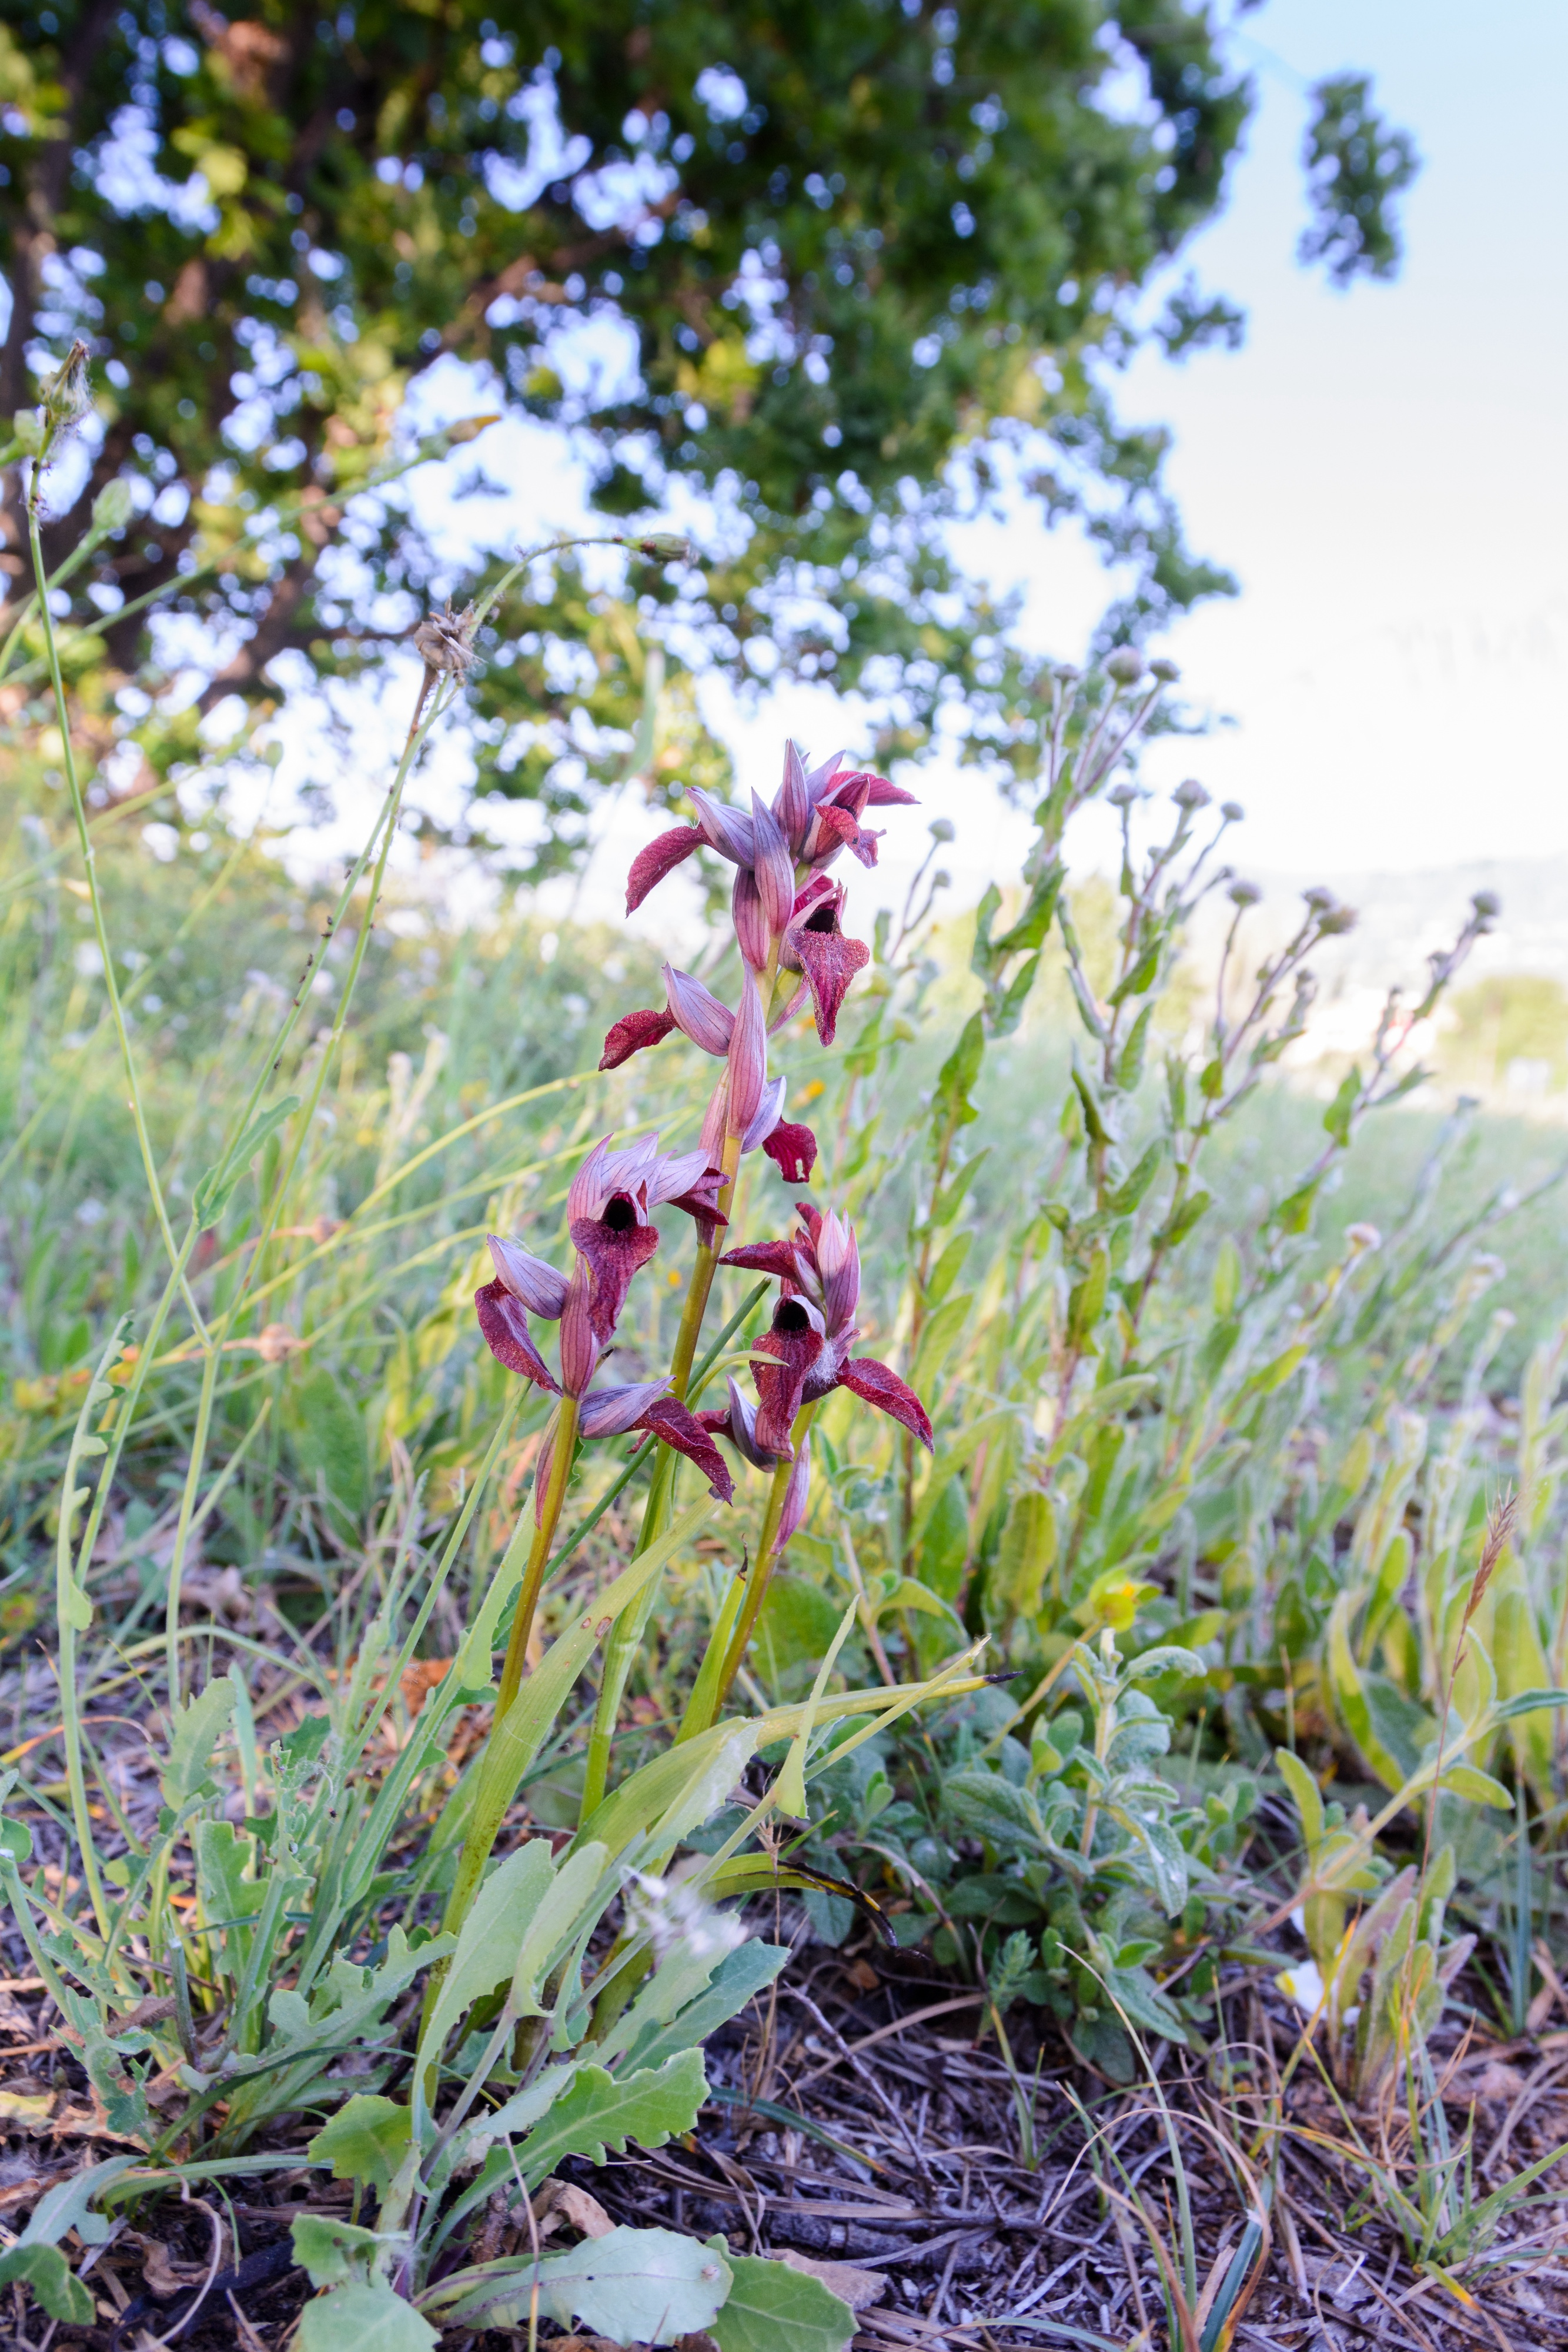
\includegraphics[keepaspectratio]{images/Serapias_cordigera_7_Giuseppe_Pellegrino.jpg}}

}

\caption{\emph{Serapias cordigera}. Foto: Guiseppe Pelligrino}

\end{figure}%

\begin{Shaded}
\begin{Highlighting}[]
\NormalTok{Serapia.eq}\OtherTok{=}\FunctionTok{clean\_names}\NormalTok{(}\FunctionTok{as.data.frame}\NormalTok{(Serapia.eq)) }\CommentTok{\# convertir la lista de matrices en un data frame y limpiar los nombres de las columnas}

\NormalTok{Serapia.eq }\SpecialCharTok{\%\textgreater{}\%} 
  \FunctionTok{gather}\NormalTok{(}\AttributeTok{key=}\StringTok{"etapa"}\NormalTok{, }\AttributeTok{value=}\StringTok{"individuos"}\NormalTok{) }\SpecialCharTok{\%\textgreater{}\%}  \CommentTok{\# convertir el data frame de formato ancho a largo}
  \FunctionTok{mutate}\NormalTok{(}\AttributeTok{etapa=}\FunctionTok{factor}\NormalTok{(etapa, }\AttributeTok{levels=}\FunctionTok{c}\NormalTok{(}\StringTok{"plantula"}\NormalTok{, }\StringTok{"latente"}\NormalTok{, }\StringTok{"rosetta"}\NormalTok{, }\StringTok{"con\_flor"}\NormalTok{))) }\SpecialCharTok{\%\textgreater{}\%} \CommentTok{\# ordenar las etapas de la vida}
  \FunctionTok{ggplot}\NormalTok{(}\FunctionTok{aes}\NormalTok{(}\AttributeTok{x=}\NormalTok{individuos))}\SpecialCharTok{+}
  \FunctionTok{geom\_histogram}\NormalTok{(}\AttributeTok{bins=}\DecValTok{30}\NormalTok{, }\FunctionTok{aes}\NormalTok{(}\AttributeTok{fill=}\StringTok{"blue"}\NormalTok{), }\AttributeTok{color=}\StringTok{"white"}\NormalTok{)}\SpecialCharTok{+}
  \FunctionTok{facet\_wrap}\NormalTok{(}\SpecialCharTok{\textasciitilde{}}\NormalTok{etapa, }\AttributeTok{scales=}\StringTok{"free"}\NormalTok{)}\SpecialCharTok{+}
  \FunctionTok{rlt\_style\_fill}\NormalTok{()}\SpecialCharTok{+}
  \FunctionTok{labs}\NormalTok{(}\AttributeTok{title=}\StringTok{"Distribución de número de individuos esperado de *Serapias cordigera*"}\NormalTok{,}
       \AttributeTok{x=}\StringTok{"Número de individuos"}\NormalTok{, }\AttributeTok{y=}\StringTok{"Frecuencia"}\NormalTok{)}\SpecialCharTok{+}
  \FunctionTok{theme}\NormalTok{(}\AttributeTok{title =} \FunctionTok{element\_markdown}\NormalTok{())}
\end{Highlighting}
\end{Shaded}

\pandocbounded{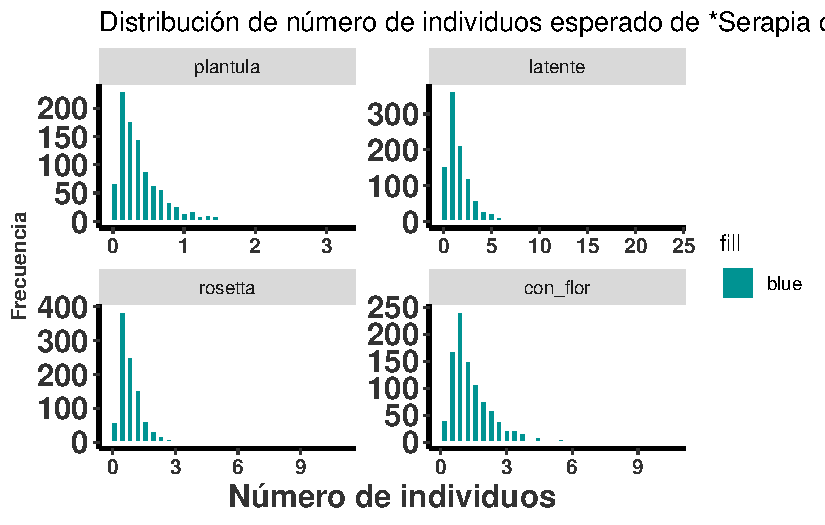
\includegraphics[keepaspectratio]{115-Metodos_de_simulaciones_files/figure-pdf/sim4-1.pdf}}

En la siguiente figura se suma el total de individuos por simulación es
una medida de la cantidad de individuos esperado en el futuro. En el
siguiente gráfico se muestra la distribución de la cantidad de
individuos esperado en el futuro de la población de \emph{Serapias
cordigera} si la especie se comporta como las matrices de transiciones
arriba y seleccionado al azar por la misma probabilidades. Se observa
que la mayoría de las simulaciones tienen menos de 10 individuos en el
futuro.

\begin{Shaded}
\begin{Highlighting}[]
\NormalTok{Serapia\_eq\_T}\OtherTok{=}\NormalTok{Serapia.eq }\SpecialCharTok{\%\textgreater{}\%} 
  \FunctionTok{mutate}\NormalTok{(}\AttributeTok{total=}\FunctionTok{rowSums}\NormalTok{(}\FunctionTok{across}\NormalTok{(}\FunctionTok{where}\NormalTok{(is.numeric)))) }\CommentTok{\# sumar la cantidad de individuos en una columna}

  
  \FunctionTok{ggplot}\NormalTok{(Serapia\_eq\_T,}\FunctionTok{aes}\NormalTok{(}\AttributeTok{x=}\NormalTok{total))}\SpecialCharTok{+}
  \FunctionTok{geom\_histogram}\NormalTok{(}\AttributeTok{bins=}\DecValTok{30}\NormalTok{, }\FunctionTok{aes}\NormalTok{(}\AttributeTok{fill=}\StringTok{"blue"}\NormalTok{), }\AttributeTok{color=}\StringTok{"white"}\NormalTok{)}\SpecialCharTok{+}
  \FunctionTok{rlt\_style\_fill}\NormalTok{()}\SpecialCharTok{+}
  \FunctionTok{labs}\NormalTok{(}\AttributeTok{title=}\StringTok{"Distribución de total de individuos esperado de *Serapias cordigera*"}\NormalTok{,}
       \AttributeTok{x=}\StringTok{"Número total de individuos por simulación"}\NormalTok{, }\AttributeTok{y=}\StringTok{"Frecuencia"}\NormalTok{)}\SpecialCharTok{+}
  \FunctionTok{theme}\NormalTok{(}\AttributeTok{title =} \FunctionTok{element\_markdown}\NormalTok{())}\SpecialCharTok{+}
    \FunctionTok{theme}\NormalTok{(}\AttributeTok{legend.position =} \StringTok{"none"}\NormalTok{)}
\end{Highlighting}
\end{Shaded}

\pandocbounded{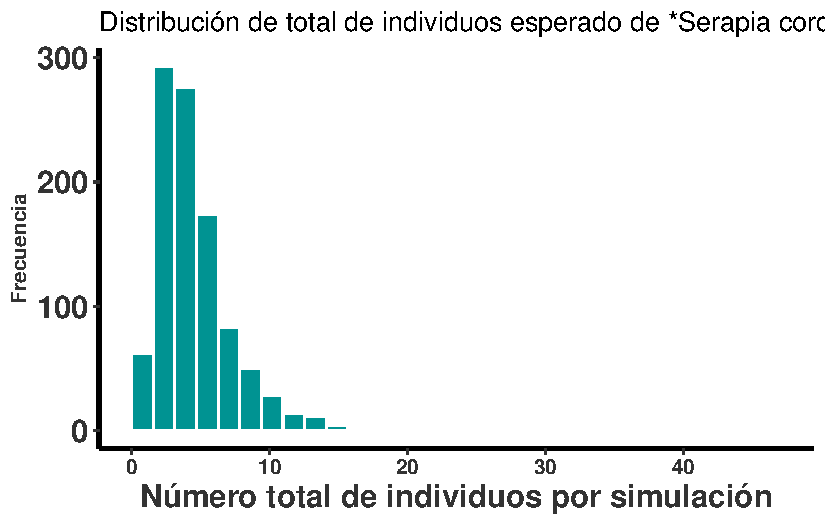
\includegraphics[keepaspectratio]{115-Metodos_de_simulaciones_files/figure-pdf/sim5-1.pdf}}

\begin{center}\rule{0.5\linewidth}{0.5pt}\end{center}

\section{Simulaciones con diferente probabilidad de
selección}\label{simulaciones-con-diferente-probabilidad-de-selecciuxf3n}

\begin{tcolorbox}[enhanced jigsaw, arc=.35mm, bottomrule=.15mm, bottomtitle=1mm, breakable, colback=white, colbacktitle=quarto-callout-tip-color!10!white, colframe=quarto-callout-tip-color-frame, coltitle=black, left=2mm, leftrule=.75mm, opacityback=0, opacitybacktitle=0.6, rightrule=.15mm, title=\textcolor{quarto-callout-tip-color}{\faLightbulb}\hspace{0.5em}{Recomendación}, titlerule=0mm, toprule=.15mm, toptitle=1mm]

\textbf{Las probabilidades de selección permiten modelar escenarios
climáticos.} Si entre las matrices disponibles algunas corresponden a
años secos y otras a años típicos, asignar mayor probabilidad de
selección a las matrices ``secas'' simula un escenario de mayor
frecuencia de sequías ---útil para evaluar respuestas poblacionales bajo
cambio climático. Lo mismo aplica para huracanes, periodos de manejo
intensivo, o cualquier evento esperado a frecuencia conocida.

\end{tcolorbox}

La probabilidad de selección de las matrices de transición no tiene que
ser igual. En el siguiente script se muestra cómo hacer simulaciones con
diferente probabilidad de selección de las matrices de transición. En
este caso se asume que las 3 poblaciones afectadas antropogénicamente
son más comunes que las poblaciones naturales. Las 3 poblaciones
naturales son raras y poco comunes. En el script vemos que ahora las
poblaciones afectadas antropogénicamente se seleccionan con una
probabilidad de 0.85 (0.30 + 0.30 + 0.25) y las poblaciones naturales
con una probabilidad de 0.15. En otras palabras, las poblaciones
naturales son muy raras y la especie está dominada por sitios donde se
ve afectada antropogénicamente. \textbf{Importante: este es una
simulación y no refleja la realidad de la especie ni de la publicación.}

\begin{Shaded}
\begin{Highlighting}[]
\NormalTok{n }\OtherTok{\textless{}{-}} \FunctionTok{c}\NormalTok{(}\DecValTok{2}\NormalTok{, }\DecValTok{0}\NormalTok{, }\DecValTok{4}\NormalTok{, }\DecValTok{99}\NormalTok{) }\CommentTok{\# población inicial por etapa}
\FunctionTok{names}\NormalTok{(n) }\OtherTok{\textless{}{-}} \FunctionTok{c}\NormalTok{(}\StringTok{"latente"}\NormalTok{, }\StringTok{"plantula"}\NormalTok{, }\StringTok{"rosetta"}\NormalTok{, }\StringTok{"con flor"}\NormalTok{)}
\NormalTok{Serapia.uneq   }\OtherTok{\textless{}{-}} \FunctionTok{stoch.projection}\NormalTok{(Serapia, n, }\AttributeTok{nreps=}\DecValTok{1000}\NormalTok{, }\AttributeTok{prob=}\FunctionTok{c}\NormalTok{(.}\DecValTok{3}\NormalTok{, .}\DecValTok{3}\NormalTok{, .}\DecValTok{25}\NormalTok{, .}\DecValTok{05}\NormalTok{, .}\DecValTok{05}\NormalTok{, .}\DecValTok{05}\NormalTok{)) }\CommentTok{\# simulación con igual probabilidad de selección}

\FunctionTok{as.data.frame}\NormalTok{(}\FunctionTok{head}\NormalTok{(Serapia.uneq)) }\SpecialCharTok{|\textgreater{}} \FunctionTok{flextable}\NormalTok{() }\CommentTok{\# vemos las primeras 6 simulaciones de tamaño de muestra}
\end{Highlighting}
\end{Shaded}

\begin{verbatim}
Error in `flextable()`:
! could not find function "flextable"
\end{verbatim}

\subsection{Comparar la distribución de cantidad de individuos esperado
por
simulaciones}\label{comparar-la-distribuciuxf3n-de-cantidad-de-individuos-esperado-por-simulaciones}

Ahora vamos a solapar las dos distribuciones (la de selección por igual
y por poblaciones mayormente impactado por humanos) para ver si hay una
diferencia en la distribución de tamaño de muestra entre las dos
simulaciones. Los resultados de la simulaciones sugieren que las
poblaciones dominadas por impacto antropogénico (rojo) tienen una mayor
cantidad de individuos en el futuro que las poblaciones bajo igualdad de
probabilidades (aquamarine).

\begin{Shaded}
\begin{Highlighting}[]
\NormalTok{Serapia.uneq}\OtherTok{=}\FunctionTok{clean\_names}\NormalTok{(}\FunctionTok{as.data.frame}\NormalTok{(Serapia.uneq))}

\NormalTok{Serapia.uneq\_T}\OtherTok{=}\NormalTok{Serapia.uneq }\SpecialCharTok{\%\textgreater{}\%} 
  \FunctionTok{mutate}\NormalTok{(}\AttributeTok{total=}\FunctionTok{rowSums}\NormalTok{(}\FunctionTok{across}\NormalTok{(}\FunctionTok{where}\NormalTok{(is.numeric)))) }

\FunctionTok{ggplot}\NormalTok{(Serapia.uneq\_T, }\FunctionTok{aes}\NormalTok{(total))}\SpecialCharTok{+}
  \FunctionTok{geom\_histogram}\NormalTok{(}\AttributeTok{bins=}\DecValTok{30}\NormalTok{, }\FunctionTok{aes}\NormalTok{(}\AttributeTok{fill=}\StringTok{"blue"}\NormalTok{), }\AttributeTok{color=}\StringTok{"white"}\NormalTok{)}\SpecialCharTok{+}
  \FunctionTok{geom\_histogram}\NormalTok{(}\AttributeTok{data=}\NormalTok{Serapia\_eq\_T, }\FunctionTok{aes}\NormalTok{(}\AttributeTok{x=}\NormalTok{total), }\AttributeTok{bins=}\DecValTok{30}\NormalTok{, }\AttributeTok{fill=}\StringTok{"aquamarine"}\NormalTok{, }\AttributeTok{color=}\StringTok{"black"}\NormalTok{, }\AttributeTok{alpha=}\NormalTok{.}\DecValTok{5}\NormalTok{)}\SpecialCharTok{+}
  \FunctionTok{rlt\_style\_fill}\NormalTok{()}\SpecialCharTok{+}
  \FunctionTok{labs}\NormalTok{(}\AttributeTok{title=}\StringTok{"Distribución del total de individuos esperado de *Serapias cordigera*"}\NormalTok{,}
       \AttributeTok{x=}\StringTok{"Número total de individuos por simulación"}\NormalTok{, }\AttributeTok{y=}\StringTok{"Frecuencia"}\NormalTok{)}\SpecialCharTok{+}
  \FunctionTok{theme}\NormalTok{(}\AttributeTok{title =} \FunctionTok{element\_markdown}\NormalTok{())}\SpecialCharTok{+}
  \FunctionTok{theme}\NormalTok{(}\AttributeTok{legend.position =} \StringTok{"none"}\NormalTok{)}
\end{Highlighting}
\end{Shaded}

\pandocbounded{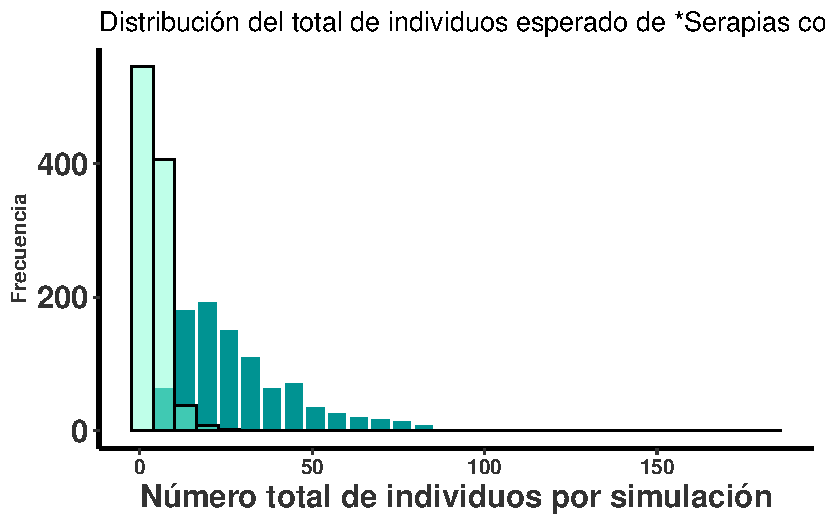
\includegraphics[keepaspectratio]{115-Metodos_de_simulaciones_files/figure-pdf/sim7-1.pdf}}

\begin{center}\rule{0.5\linewidth}{0.5pt}\end{center}

\subsubsection{\texorpdfstring{Simulación de crecimiento poblacional de
\emph{Serapias
cordigera}}{Simulación de crecimiento poblacional de Serapias cordigera}}\label{simulaciuxf3n-de-crecimiento-poblacional-de-serapias-cordigera}

En el siguiente script podemos evaluar el crecimiento poblacional y su
variación en el espacio.

Nota: aquí se calcula el log del crecimiento poblacional estocástico de
\emph{Serapias cordigera} por aproximación y simulaciones siguiendo la
fórmula de Tuljapurkar (Tuljapurkar, 2013). Se puede ver que la especie
tiene un crecimiento poblacional negativo en la mayoría de las
simulaciones. Esto sugiere que la especie está en declive. Pero también
se puede ver que hay variación en el crecimiento poblacional de la
especie. El script incluye un parámetro para indicar por cuánto tiempo
queremos que la simulación ocurra, \textbf{maxt=}; en este caso se
simula por 50 periodos de tiempo. Si no se añade nada, la simulación
dura por 50000 periodos de tiempo. Nota que \textbf{maxt} es en la
unidad de tiempo de la matriz de transición; si esta fue construida en
un periodo de meses, entonces la simulación opera en ese intervalo de
tiempo.

Cuando se usa el log de crecimiento poblacional estocástico se calcula
\(r\), donde \(r = \ln(\lambda)\). La interpretación de \(r\) es
distinta a la de \(\lambda\):

\begin{itemize}
\tightlist
\item
  \(r\) = log(crecimiento poblacional estocástico) \textgreater{} 0 la
  población crece
\item
  \(r\) = log(crecimiento poblacional estocástico) \textless{} 0 la
  población decrece
\item
  \(r\) = log(crecimiento poblacional estocástico) = 0 la población es
  estable
\end{itemize}

El crecimiento estocástico de las poblaciones de \emph{Serapias
cordigera} en 1999 es negativo, lo que sugiere que la especie está en
declive. Pero también se puede ver que hay variación en el crecimiento
poblacional de la especie. Se usa la función
\texttt{stoch.growth.rate()}.

Simulaciones por selección de matriz con igual probabilidad

\begin{itemize}
\tightlist
\item
  el crecimiento es negativo y los intervalos de confianza también,
  dando confianza de que la especie está en declive.
\end{itemize}

\begin{Shaded}
\begin{Highlighting}[]
\NormalTok{SGR\_eq}\OtherTok{=}\FunctionTok{stoch.growth.rate}\NormalTok{(Serapia, }\AttributeTok{maxt=}\DecValTok{50}\NormalTok{, }\AttributeTok{verbose=}\ConstantTok{TRUE}\NormalTok{) }\CommentTok{\# matrices seleccionado con igual probabilidad}
\NormalTok{SGR\_eq}
\end{Highlighting}
\end{Shaded}

\begin{verbatim}
$approx
[1] -0.06760619

$sim
[1] -0.04498096

$sim.CI
[1] -0.07640695 -0.01355498
\end{verbatim}

\begin{center}\rule{0.5\linewidth}{0.5pt}\end{center}

\subsection{Simulaciones por selección de matriz con diferente
probabilidad}\label{simulaciones-por-selecciuxf3n-de-matriz-con-diferente-probabilidad}

\begin{itemize}
\tightlist
\item
  el crecimiento es negativo y los intervalos de confianza solapan el
  cero, lo que sugiere que hay variación en el crecimiento poblacional
  de la especie y que no hay evidencia de que la especie esté en declive
  ni aumentando (es estable). La interpretación aquí es que, si la
  especie está dominada por poblaciones con impacto antropogénico, tiene
  un crecimiento poblacional no negativo.
\end{itemize}

\begin{Shaded}
\begin{Highlighting}[]
\NormalTok{SGR\_uneq}\OtherTok{=}\FunctionTok{stoch.growth.rate}\NormalTok{(Serapia, }\AttributeTok{maxt=}\DecValTok{50}\NormalTok{, }\AttributeTok{prob=}\FunctionTok{c}\NormalTok{(.}\DecValTok{3}\NormalTok{, .}\DecValTok{3}\NormalTok{, .}\DecValTok{25}\NormalTok{, .}\DecValTok{05}\NormalTok{, .}\DecValTok{05}\NormalTok{, .}\DecValTok{05}\NormalTok{), }\AttributeTok{verbose=}\ConstantTok{FALSE}\NormalTok{) }\CommentTok{\# matrices seleccionado con diferente probabilidades}

\NormalTok{SGR\_uneq}
\end{Highlighting}
\end{Shaded}

\begin{verbatim}
$approx
[1] -0.02988694

$sim
[1] -0.01902192

$sim.CI
[1] -0.05012701  0.01208317
\end{verbatim}

Para convertir el log(crecimiento poblacional estocástico) a lambda se
usa la siguiente formula \(e^r\) donde \(r\) es el log(crecimiento
poblacional estocástico). Como ejemplo se muestra la metodología con las
simulaciones con probabilidad desigual de selección de las matrices de
transición.

\begin{tcolorbox}[enhanced jigsaw, arc=.35mm, bottomrule=.15mm, bottomtitle=1mm, breakable, colback=white, colbacktitle=quarto-callout-note-color!10!white, colframe=quarto-callout-note-color-frame, coltitle=black, left=2mm, leftrule=.75mm, opacityback=0, opacitybacktitle=0.6, rightrule=.15mm, title=\textcolor{quarto-callout-note-color}{\faInfo}\hspace{0.5em}{Nota}, titlerule=0mm, toprule=.15mm, toptitle=1mm]

\textbf{Por qué \texttt{stoch.growth.rate()} reporta \(\log \lambda_s\)
y no \(\lambda_s\) directamente.} Cuando una población crece
estocásticamente, la \textbf{media geométrica} del crecimiento (no la
aritmética) es el predictor correcto del tamaño futuro. La media
geométrica de \(\lambda\) se calcula como
\(\exp(\overline{\log \lambda})\). Por eso conviene trabajar en escala
logarítmica internamente y convertir a λ con \texttt{exp()} solo al
reportar. Si los intervalos de confianza incluyen 0 en la escala log,
son equivalentes a incluir 1 en la escala λ --- es decir, no hay
evidencia de crecimiento ni declive.

\end{tcolorbox}

\subsubsection{\texorpdfstring{Conversión de \(r\) a
\(\lambda\)}{Conversión de r a \textbackslash lambda}}\label{conversiuxf3n-de-r-a-lambda}

Lambda Igual de probabilidades

\begin{Shaded}
\begin{Highlighting}[]
\FunctionTok{exp}\NormalTok{(SGR\_uneq}\SpecialCharTok{$}\NormalTok{sim) }\CommentTok{\# matrices seleccionado con igual probabilidad}
\end{Highlighting}
\end{Shaded}

\begin{verbatim}
[1] 0.9811579
\end{verbatim}

\begin{Shaded}
\begin{Highlighting}[]
\FunctionTok{exp}\NormalTok{(SGR\_uneq}\SpecialCharTok{$}\NormalTok{sim.CI[}\DecValTok{1}\NormalTok{]) }\CommentTok{\#El intervalo de confianza inferior}
\end{Highlighting}
\end{Shaded}

\begin{verbatim}
[1] 0.9511086
\end{verbatim}

\begin{Shaded}
\begin{Highlighting}[]
\FunctionTok{exp}\NormalTok{(SGR\_uneq}\SpecialCharTok{$}\NormalTok{sim.CI[}\DecValTok{2}\NormalTok{]) }\CommentTok{\#El intervalo de confianza superior}
\end{Highlighting}
\end{Shaded}

\begin{verbatim}
[1] 1.012156
\end{verbatim}

\begin{center}\rule{0.5\linewidth}{0.5pt}\end{center}

\subsection{Impacto antropogénico vs poblaciones
naturales}\label{impacto-antropoguxe9nico-vs-poblaciones-naturales}

Los análisis anteriores no separan las matrices de transición por el
impacto antropogénico versus las poblaciones naturales. En el siguiente
script se muestra como hacer simulaciones y estimar el crecimiento
poblacional de las poblaciones afectada de forma separada.

\begin{itemize}
\tightlist
\item
  Separamos las matrices de transición en dos grupos, uno para las
  poblaciones afectada de forma antropogénicas y otro para las
  poblaciones naturales.
\end{itemize}

\begin{Shaded}
\begin{Highlighting}[]
\NormalTok{Serapia\_A }\OtherTok{=}\NormalTok{ Serapia[}\DecValTok{1}\SpecialCharTok{:}\DecValTok{3}\NormalTok{] }\CommentTok{\# poblaciones afectada de forma antropogénicas}

\NormalTok{Serapia\_N}\OtherTok{=}\NormalTok{  Serapia[}\DecValTok{4}\SpecialCharTok{:}\DecValTok{6}\NormalTok{] }\CommentTok{\# poblaciones naturales}
\end{Highlighting}
\end{Shaded}

Asumimos una probabilidad igual de selección por cada simulaciones en
ambos escenarios

\begin{Shaded}
\begin{Highlighting}[]
\NormalTok{n }\OtherTok{\textless{}{-}} \FunctionTok{c}\NormalTok{(}\DecValTok{2}\NormalTok{, }\DecValTok{0}\NormalTok{, }\DecValTok{4}\NormalTok{, }\DecValTok{99}\NormalTok{) }\CommentTok{\# corresponde a los datos de la especie en la publicación del año 2000}
\FunctionTok{names}\NormalTok{(n) }\OtherTok{\textless{}{-}} \FunctionTok{c}\NormalTok{(}\StringTok{"latente"}\NormalTok{, }\StringTok{"plantula"}\NormalTok{, }\StringTok{"rosetta"}\NormalTok{, }\StringTok{"con flor"}\NormalTok{)}
\NormalTok{Serapia.eq\_A   }\OtherTok{\textless{}{-}} \FunctionTok{stoch.projection}\NormalTok{(Serapia\_A, n, }\AttributeTok{nreps=}\DecValTok{1000}\NormalTok{)}
\NormalTok{Serapia.eq\_N   }\OtherTok{\textless{}{-}} \FunctionTok{stoch.projection}\NormalTok{(Serapia\_N, n, }\AttributeTok{nreps=}\DecValTok{1000}\NormalTok{)}
\end{Highlighting}
\end{Shaded}

Convertir las simulaciones de las matrices de transición en un data
frame y limpiar los nombres de las columnas. Luego sumar el total de
individuos por simulación para cada etapa de la vida. Esto es necesario
para poder visualizar el tamaño poblacional esperado por etapa de la
vida. El resultado del análisis es que las poblaciones afectada de forma
antropogénicas tienen un estimado de tamaño de poblacional más grande
que las poblaciones naturales.

\begin{Shaded}
\begin{Highlighting}[]
\NormalTok{Serapia.eq\_A}\OtherTok{=}\FunctionTok{clean\_names}\NormalTok{(}\FunctionTok{as.data.frame}\NormalTok{(Serapia.eq\_A)) }\CommentTok{\# limpiar los nombres de las columnas y convertir en un data frame}
\NormalTok{Serapia.eq\_N}\OtherTok{=}\FunctionTok{clean\_names}\NormalTok{(}\FunctionTok{as.data.frame}\NormalTok{(Serapia.eq\_N)) }

\NormalTok{Serapia\_eq\_A}\OtherTok{=}\NormalTok{Serapia.eq\_A }\SpecialCharTok{\%\textgreater{}\%} 
  \FunctionTok{mutate}\NormalTok{(}\AttributeTok{total=}\FunctionTok{rowSums}\NormalTok{(}\FunctionTok{across}\NormalTok{(}\FunctionTok{where}\NormalTok{(is.numeric)))) }\CommentTok{\# sumar la cantidad de individuos en una columna}

\NormalTok{Serapia\_eq\_N}\OtherTok{=}\NormalTok{Serapia.eq\_N }\SpecialCharTok{\%\textgreater{}\%} 
  \FunctionTok{mutate}\NormalTok{(}\AttributeTok{total=}\FunctionTok{rowSums}\NormalTok{(}\FunctionTok{across}\NormalTok{(}\FunctionTok{where}\NormalTok{(is.numeric))))}
\end{Highlighting}
\end{Shaded}

Visualizar el tamaño de poblacional esperado por etapa de la vida para
las poblaciones afectada de forma antropogénicas y naturales. Se observa
que las poblaciones afectada de forma antropogénicas tienen un tamaño de
poblacional más grande que las poblaciones naturales. la poblaciones con
efecto antropogénico tienen a ser de mayor cantidad.

\begin{Shaded}
\begin{Highlighting}[]
\NormalTok{diverging}\OtherTok{=} \FunctionTok{c}\NormalTok{(}\StringTok{"\#009392"}\NormalTok{,}\StringTok{"\#CF597E"}\NormalTok{,}\StringTok{"\#E9E29C"}\NormalTok{, }\StringTok{"\#39B185"}\NormalTok{,}\StringTok{"\#EEB479"}\NormalTok{ , }\StringTok{"\#9CCB86"}\NormalTok{ )}
\FunctionTok{ggplot}\NormalTok{(Serapia\_eq\_N, }\FunctionTok{aes}\NormalTok{(total))}\SpecialCharTok{+}
  \FunctionTok{geom\_histogram}\NormalTok{(}\AttributeTok{fill=} \StringTok{"\#009392"}\NormalTok{, }\AttributeTok{color=}\StringTok{"white"}\NormalTok{,}\AttributeTok{bins=}\DecValTok{30}\NormalTok{,  }\AttributeTok{alpha=}\NormalTok{.}\DecValTok{5}\NormalTok{)}\SpecialCharTok{+}
  \FunctionTok{geom\_histogram}\NormalTok{(}\AttributeTok{data=}\NormalTok{Serapia\_eq\_A, }\FunctionTok{aes}\NormalTok{(}\AttributeTok{x=}\NormalTok{total), }
                \AttributeTok{fill=}\StringTok{"\#CF597E"}\NormalTok{, }\AttributeTok{color=}\StringTok{"white"}\NormalTok{, }\AttributeTok{bins=}\DecValTok{30}\NormalTok{,  }\AttributeTok{alpha=}\NormalTok{.}\DecValTok{5}\NormalTok{)}\SpecialCharTok{+}
  \FunctionTok{theme\_minimal}\NormalTok{()}\SpecialCharTok{+}
  \FunctionTok{labs}\NormalTok{(}\AttributeTok{title=}\StringTok{"Distribución de total de individuos esperado de *Serapias cordigera*"}\NormalTok{,}
       \AttributeTok{x=}\StringTok{"Número total de individuos por simulación"}\NormalTok{, }\AttributeTok{y=}\StringTok{"Frecuencia"}\NormalTok{)}\SpecialCharTok{+}
  \FunctionTok{theme}\NormalTok{(}\AttributeTok{title =} \FunctionTok{element\_markdown}\NormalTok{())}
\end{Highlighting}
\end{Shaded}

\pandocbounded{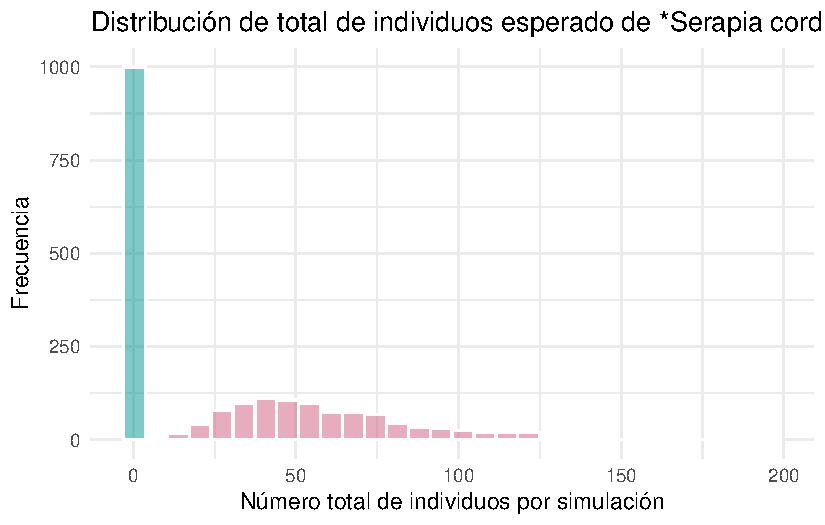
\includegraphics[keepaspectratio]{115-Metodos_de_simulaciones_files/figure-pdf/unnamed-chunk-2-1.pdf}}

\begin{center}\rule{0.5\linewidth}{0.5pt}\end{center}

\section{Estocasticidad temporal}\label{estocasticidad-temporal}

\begin{figure}[H]

{\centering \pandocbounded{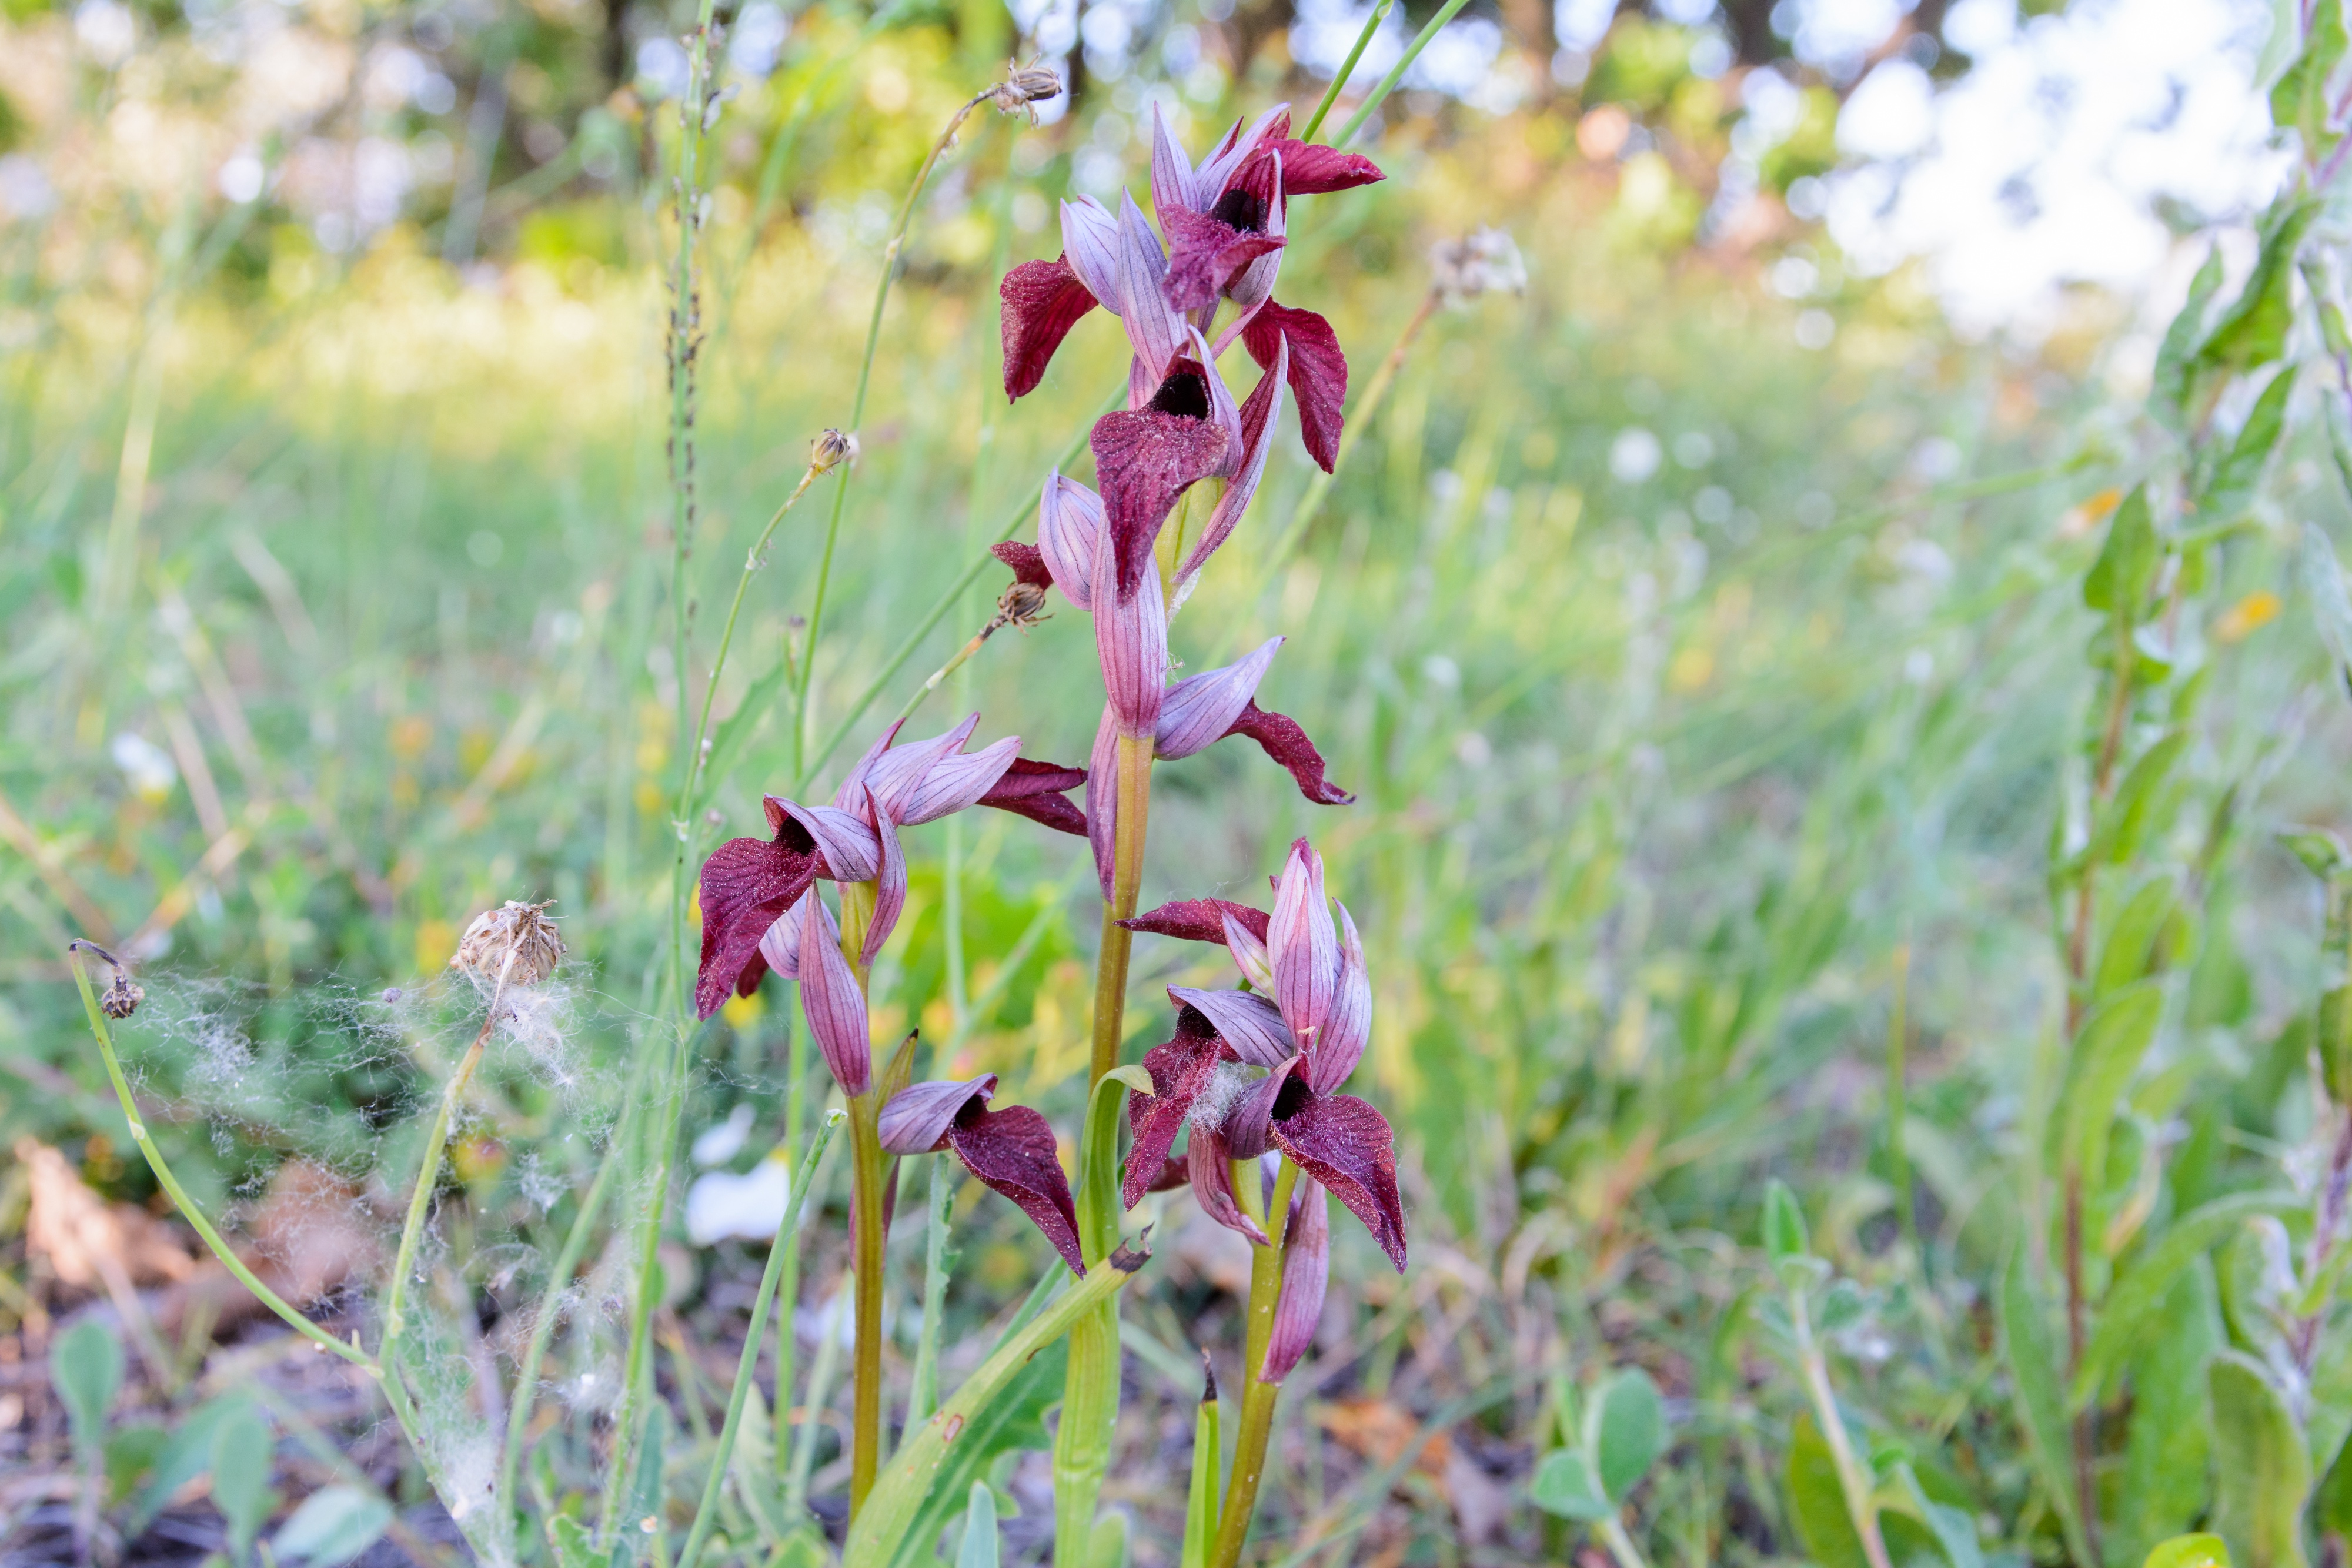
\includegraphics[keepaspectratio]{images/Serapias_cordigera_3_Giuseppe_Pellegrino.jpeg}}

}

\caption{\emph{Serapias cordigera}. Foto: Guiseppe Pelligrino}

\end{figure}%

El objetivo de evaluar la variación en tiempo es para determinar si los
efectos temporales son importante en predecir los cambios en el
crecimiento o estabilidad poblacional. Seguimos con los datos
\emph{Serapias cordigera}, pero ahora evaluamos cual es el efecto de la
variación en los parámetros de la matriz usando múltiple censos. Vemos
el efecto de una esas población, por impacto antropogénico solamente de
la población \textbf{A1} en los 13 años de muestreo comenzando en el
1999 al 2011, inclusivo.

El primer paso en entrar los datos en una lista de matrices de
transición.

\begin{Shaded}
\begin{Highlighting}[]
\NormalTok{Serapia\_tiempo}\OtherTok{\textless{}{-}}\FunctionTok{list}\NormalTok{(}
  \AttributeTok{A1\_1999=}\FunctionTok{matrix}\NormalTok{(}\FunctionTok{c}\NormalTok{(}
\FloatTok{0.745}\NormalTok{,  }\FloatTok{0.152}\NormalTok{,  }\FloatTok{0.452}\NormalTok{,  }\FloatTok{0.564}\NormalTok{,}
\FloatTok{0.125}\NormalTok{,  }\FloatTok{0.000}\NormalTok{,  }\FloatTok{0.000}\NormalTok{,  }\FloatTok{0.000}\NormalTok{,}
\FloatTok{0.000}\NormalTok{,  }\FloatTok{0.321}\NormalTok{,  }\FloatTok{0.205}\NormalTok{,  }\FloatTok{0.342}\NormalTok{,}
\FloatTok{0.200}\NormalTok{,  }\FloatTok{0.365}\NormalTok{,  }\FloatTok{0.205}\NormalTok{,  }\FloatTok{0.185}
\NormalTok{  ),}
  \AttributeTok{nrow=}\DecValTok{4}\NormalTok{, }\AttributeTok{byrow=}\ConstantTok{TRUE}\NormalTok{,}
  \AttributeTok{dimnames=}\FunctionTok{list}\NormalTok{(}\FunctionTok{c}\NormalTok{(}\StringTok{"latente"}\NormalTok{, }\StringTok{"plantula"}\NormalTok{, }\StringTok{"rosetta"}\NormalTok{, }\StringTok{"con flor"}\NormalTok{),}
                \FunctionTok{c}\NormalTok{(}\StringTok{"latente"}\NormalTok{, }\StringTok{"plantula"}\NormalTok{, }\StringTok{"rosetta"}\NormalTok{, }\StringTok{"con flor"}\NormalTok{)}
\NormalTok{  )}
\NormalTok{  ),}
\AttributeTok{A1\_2000=}\FunctionTok{matrix}\NormalTok{(}\FunctionTok{c}\NormalTok{(}
\FloatTok{0.578}\NormalTok{,  }\FloatTok{0.222}\NormalTok{,  }\FloatTok{0.394}\NormalTok{,  }\FloatTok{0.394}\NormalTok{,}
\FloatTok{0.188}\NormalTok{   ,}\FloatTok{0.000}\NormalTok{, }\FloatTok{0.000}\NormalTok{,  }\FloatTok{0.000}\NormalTok{,}
\FloatTok{0.000}\NormalTok{   ,}\FloatTok{0.322}\NormalTok{, }\FloatTok{0.254}\NormalTok{,  }\FloatTok{0.357}\NormalTok{,}
\FloatTok{0.244}\NormalTok{   ,}\FloatTok{0.314}\NormalTok{, }\FloatTok{0.125}\NormalTok{,  }\FloatTok{0.302}
\NormalTok{  ),}
  \AttributeTok{nrow=}\DecValTok{4}\NormalTok{, }\AttributeTok{byrow=}\ConstantTok{TRUE}\NormalTok{,}
  \AttributeTok{dimnames=}\FunctionTok{list}\NormalTok{(}\FunctionTok{c}\NormalTok{(}\StringTok{"latente"}\NormalTok{, }\StringTok{"plantula"}\NormalTok{, }\StringTok{"rosetta"}\NormalTok{, }\StringTok{"con flor"}\NormalTok{),}
                \FunctionTok{c}\NormalTok{(}\StringTok{"latente"}\NormalTok{, }\StringTok{"plantula"}\NormalTok{, }\StringTok{"rosetta"}\NormalTok{, }\StringTok{"con flor"}\NormalTok{)}
\NormalTok{  )}
\NormalTok{  ),}
\AttributeTok{A1\_2001=}\FunctionTok{matrix}\NormalTok{(}\FunctionTok{c}\NormalTok{(}
  \FloatTok{0.668}\NormalTok{,    }\FloatTok{0.122}\NormalTok{,  }\FloatTok{0.294}\NormalTok{,  }\FloatTok{0.401}\NormalTok{,}
\FloatTok{0.128}\NormalTok{,  }\FloatTok{0.000}\NormalTok{   ,}\FloatTok{0.000}\NormalTok{, }\FloatTok{0.000}\NormalTok{,}
\FloatTok{0.000}\NormalTok{,  }\FloatTok{0.302}\NormalTok{   ,}\FloatTok{0.453}\NormalTok{, }\FloatTok{0.366}\NormalTok{,}
\FloatTok{0.214}\NormalTok{,  }\FloatTok{0.364}\NormalTok{,  }\FloatTok{0.185}\NormalTok{,  }\FloatTok{0.207}
\NormalTok{  ),}
  \AttributeTok{nrow=}\DecValTok{4}\NormalTok{, }\AttributeTok{byrow=}\ConstantTok{TRUE}\NormalTok{,}
  \AttributeTok{dimnames=}\FunctionTok{list}\NormalTok{(}\FunctionTok{c}\NormalTok{(}\StringTok{"latente"}\NormalTok{, }\StringTok{"plantula"}\NormalTok{, }\StringTok{"rosetta"}\NormalTok{, }\StringTok{"con flor"}\NormalTok{),}
                \FunctionTok{c}\NormalTok{(}\StringTok{"latente"}\NormalTok{, }\StringTok{"plantula"}\NormalTok{, }\StringTok{"rosetta"}\NormalTok{, }\StringTok{"con flor"}\NormalTok{)}
\NormalTok{  )}
\NormalTok{  ),}
\AttributeTok{A1\_2002=}\FunctionTok{matrix}\NormalTok{(}\FunctionTok{c}\NormalTok{(}
\FloatTok{0.645}\NormalTok{,  }\FloatTok{0.222}\NormalTok{,  }\FloatTok{0.682}\NormalTok{,  }\FloatTok{0.504}\NormalTok{,}
\FloatTok{0.177}\NormalTok{,  }\FloatTok{0.000}\NormalTok{,  }\FloatTok{0.000}\NormalTok{,  }\FloatTok{0.000}\NormalTok{,}
\FloatTok{0.000}\NormalTok{,  }\FloatTok{0.421}\NormalTok{,  }\FloatTok{0.305}\NormalTok{,  }\FloatTok{0.382}\NormalTok{,}
\FloatTok{0.102}\NormalTok{,  }\FloatTok{0.355}\NormalTok{,  }\FloatTok{0.208}\NormalTok{,  }\FloatTok{0.208}
\NormalTok{  ),}
  \AttributeTok{nrow=}\DecValTok{4}\NormalTok{, }\AttributeTok{byrow=}\ConstantTok{TRUE}\NormalTok{,}
  \AttributeTok{dimnames=}\FunctionTok{list}\NormalTok{(}\FunctionTok{c}\NormalTok{(}\StringTok{"latente"}\NormalTok{, }\StringTok{"plantula"}\NormalTok{, }\StringTok{"rosetta"}\NormalTok{, }\StringTok{"con flor"}\NormalTok{),}
                \FunctionTok{c}\NormalTok{(}\StringTok{"latente"}\NormalTok{, }\StringTok{"plantula"}\NormalTok{, }\StringTok{"rosetta"}\NormalTok{, }\StringTok{"con flor"}\NormalTok{)}
\NormalTok{  )}
\NormalTok{  ),}
\AttributeTok{A1\_2003=}\FunctionTok{matrix}\NormalTok{(}\FunctionTok{c}\NormalTok{(}
  \FloatTok{0.545}\NormalTok{,    }\FloatTok{0.113}\NormalTok{,  }\FloatTok{0.424}\NormalTok{,  }\FloatTok{0.424}\NormalTok{,}
\FloatTok{0.247}\NormalTok{,  }\FloatTok{0.000}\NormalTok{,  }\FloatTok{0.000}\NormalTok{,  }\FloatTok{0.000}\NormalTok{,}
\FloatTok{0.000}\NormalTok{,  }\FloatTok{0.166}\NormalTok{,  }\FloatTok{0.233}\NormalTok{,  }\FloatTok{0.277}\NormalTok{,}
\FloatTok{0.192}\NormalTok{,  }\FloatTok{0.253}\NormalTok{,  }\FloatTok{0.209}\NormalTok{,  }\FloatTok{0.212}

\NormalTok{  ),}
  \AttributeTok{nrow=}\DecValTok{4}\NormalTok{, }\AttributeTok{byrow=}\ConstantTok{TRUE}\NormalTok{,}
  \AttributeTok{dimnames=}\FunctionTok{list}\NormalTok{(}\FunctionTok{c}\NormalTok{(}\StringTok{"latente"}\NormalTok{, }\StringTok{"plantula"}\NormalTok{, }\StringTok{"rosetta"}\NormalTok{, }\StringTok{"con flor"}\NormalTok{),}
                \FunctionTok{c}\NormalTok{(}\StringTok{"latente"}\NormalTok{, }\StringTok{"plantula"}\NormalTok{, }\StringTok{"rosetta"}\NormalTok{, }\StringTok{"con flor"}\NormalTok{)}
\NormalTok{  )}
\NormalTok{  ),}
\AttributeTok{A1\_2004=}\FunctionTok{matrix}\NormalTok{(}\FunctionTok{c}\NormalTok{(}
  \FloatTok{0.548}\NormalTok{,    }\FloatTok{0.191}\NormalTok{,  }\FloatTok{0.402}\NormalTok{,  }\FloatTok{0.527}\NormalTok{,}
\FloatTok{0.327}\NormalTok{,  }\FloatTok{0.000}\NormalTok{,  }\FloatTok{0.000}\NormalTok{,  }\FloatTok{0.000}\NormalTok{,}
\FloatTok{0.000}\NormalTok{,  }\FloatTok{0.338}\NormalTok{,  }\FloatTok{0.127}\NormalTok{,  }\FloatTok{0.394}\NormalTok{,}
\FloatTok{0.211}\NormalTok{,  }\FloatTok{0.262}\NormalTok{,  }\FloatTok{0.296}\NormalTok{,  }\FloatTok{0.142}
\NormalTok{  ),}
  \AttributeTok{nrow=}\DecValTok{4}\NormalTok{, }\AttributeTok{byrow=}\ConstantTok{TRUE}\NormalTok{,}
  \AttributeTok{dimnames=}\FunctionTok{list}\NormalTok{(}\FunctionTok{c}\NormalTok{(}\StringTok{"latente"}\NormalTok{, }\StringTok{"plantula"}\NormalTok{, }\StringTok{"rosetta"}\NormalTok{, }\StringTok{"con flor"}\NormalTok{),}
                \FunctionTok{c}\NormalTok{(}\StringTok{"latente"}\NormalTok{, }\StringTok{"plantula"}\NormalTok{, }\StringTok{"rosetta"}\NormalTok{, }\StringTok{"con flor"}\NormalTok{)}
\NormalTok{  )}
\NormalTok{  ),}
\AttributeTok{A1\_2005=}\FunctionTok{matrix}\NormalTok{(}\FunctionTok{c}\NormalTok{(}
  \FloatTok{0.602}\NormalTok{,    }\FloatTok{0.153}\NormalTok{,  }\FloatTok{0.486}\NormalTok{,  }\FloatTok{0.562}\NormalTok{,}
\FloatTok{0.224}\NormalTok{,  }\FloatTok{0.000}\NormalTok{,  }\FloatTok{0.000}\NormalTok{,  }\FloatTok{0.000}\NormalTok{,}
\FloatTok{0.000}\NormalTok{,  }\FloatTok{0.491}\NormalTok{,  }\FloatTok{0.324}\NormalTok{,  }\FloatTok{0.304}\NormalTok{,}
\FloatTok{0.139}\NormalTok{,  }\FloatTok{0.268}\NormalTok{,  }\FloatTok{0.294}\NormalTok{,  }\FloatTok{0.277}

\NormalTok{  ),}
  \AttributeTok{nrow=}\DecValTok{4}\NormalTok{, }\AttributeTok{byrow=}\ConstantTok{TRUE}\NormalTok{,}
  \AttributeTok{dimnames=}\FunctionTok{list}\NormalTok{(}\FunctionTok{c}\NormalTok{(}\StringTok{"latente"}\NormalTok{, }\StringTok{"plantula"}\NormalTok{, }\StringTok{"rosetta"}\NormalTok{, }\StringTok{"con flor"}\NormalTok{),}
                \FunctionTok{c}\NormalTok{(}\StringTok{"latente"}\NormalTok{, }\StringTok{"plantula"}\NormalTok{, }\StringTok{"rosetta"}\NormalTok{, }\StringTok{"con flor"}\NormalTok{)}
\NormalTok{  )}
\NormalTok{  ),}
\AttributeTok{A1\_2006=}\FunctionTok{matrix}\NormalTok{(}\FunctionTok{c}\NormalTok{(}
  \FloatTok{0.487}\NormalTok{,    }\FloatTok{0.471}\NormalTok{,  }\FloatTok{0.425}\NormalTok{,  }\FloatTok{0.607}\NormalTok{,}
\FloatTok{0.318}\NormalTok{,  }\FloatTok{0.000}\NormalTok{,  }\FloatTok{0.000}\NormalTok{,  }\FloatTok{0.000}\NormalTok{,}
\FloatTok{0.000}\NormalTok{,  }\FloatTok{0.438}\NormalTok{,  }\FloatTok{0.328}\NormalTok{,  }\FloatTok{0.373}\NormalTok{,}
\FloatTok{0.211}\NormalTok{,  }\FloatTok{0.212}\NormalTok{,  }\FloatTok{0.285}\NormalTok{,  }\FloatTok{0.142}
\NormalTok{  ),}
  \AttributeTok{nrow=}\DecValTok{4}\NormalTok{, }\AttributeTok{byrow=}\ConstantTok{TRUE}\NormalTok{,}
  \AttributeTok{dimnames=}\FunctionTok{list}\NormalTok{(}\FunctionTok{c}\NormalTok{(}\StringTok{"latente"}\NormalTok{, }\StringTok{"plantula"}\NormalTok{, }\StringTok{"rosetta"}\NormalTok{, }\StringTok{"con flor"}\NormalTok{),}
                \FunctionTok{c}\NormalTok{(}\StringTok{"latente"}\NormalTok{, }\StringTok{"plantula"}\NormalTok{, }\StringTok{"rosetta"}\NormalTok{, }\StringTok{"con flor"}\NormalTok{)}
\NormalTok{  )}
\NormalTok{  ),}
\AttributeTok{A1\_2007=}\FunctionTok{matrix}\NormalTok{(}\FunctionTok{c}\NormalTok{(}
  \FloatTok{0.544}\NormalTok{,    }\FloatTok{0.423}\NormalTok{,  }\FloatTok{0.374}\NormalTok{,  }\FloatTok{0.578}\NormalTok{,}
\FloatTok{0.348}\NormalTok{,  }\FloatTok{0.000}\NormalTok{,  }\FloatTok{0.000}\NormalTok{,  }\FloatTok{0.000}\NormalTok{,}
\FloatTok{0.000}\NormalTok{,  }\FloatTok{0.441}\NormalTok{,  }\FloatTok{0.248}\NormalTok{,  }\FloatTok{0.288}\NormalTok{,}
\FloatTok{0.145}\NormalTok{,  }\FloatTok{0.203}\NormalTok{,  }\FloatTok{0.311}\NormalTok{,  }\FloatTok{0.201}

\NormalTok{  ),}
  \AttributeTok{nrow=}\DecValTok{4}\NormalTok{, }\AttributeTok{byrow=}\ConstantTok{TRUE}\NormalTok{,}
  \AttributeTok{dimnames=}\FunctionTok{list}\NormalTok{(}\FunctionTok{c}\NormalTok{(}\StringTok{"latente"}\NormalTok{, }\StringTok{"plantula"}\NormalTok{, }\StringTok{"rosetta"}\NormalTok{, }\StringTok{"con flor"}\NormalTok{),}
                \FunctionTok{c}\NormalTok{(}\StringTok{"latente"}\NormalTok{, }\StringTok{"plantula"}\NormalTok{, }\StringTok{"rosetta"}\NormalTok{, }\StringTok{"con flor"}\NormalTok{)}
\NormalTok{  )}
\NormalTok{  ),}
\AttributeTok{A1\_2008=}\FunctionTok{matrix}\NormalTok{(}\FunctionTok{c}\NormalTok{(}
 \FloatTok{0.568}\NormalTok{, }\FloatTok{0.325}\NormalTok{,  }\FloatTok{0.294}\NormalTok{,  }\FloatTok{0.607}\NormalTok{,}
\FloatTok{0.227}\NormalTok{,  }\FloatTok{0.000}\NormalTok{,  }\FloatTok{0.000}\NormalTok{,  }\FloatTok{0.000}\NormalTok{,}
\FloatTok{0.000}\NormalTok{,  }\FloatTok{0.402}\NormalTok{,  }\FloatTok{0.553}\NormalTok{,  }\FloatTok{0.256}\NormalTok{,}
\FloatTok{0.194}\NormalTok{,  }\FloatTok{0.364}\NormalTok{,  }\FloatTok{0.275}\NormalTok{,  }\FloatTok{0.217}

\NormalTok{  ),}
  \AttributeTok{nrow=}\DecValTok{4}\NormalTok{, }\AttributeTok{byrow=}\ConstantTok{TRUE}\NormalTok{,}
  \AttributeTok{dimnames=}\FunctionTok{list}\NormalTok{(}\FunctionTok{c}\NormalTok{(}\StringTok{"latente"}\NormalTok{, }\StringTok{"plantula"}\NormalTok{, }\StringTok{"rosetta"}\NormalTok{, }\StringTok{"con flor"}\NormalTok{),}
                \FunctionTok{c}\NormalTok{(}\StringTok{"latente"}\NormalTok{, }\StringTok{"plantula"}\NormalTok{, }\StringTok{"rosetta"}\NormalTok{, }\StringTok{"con flor"}\NormalTok{)}
\NormalTok{  )}
\NormalTok{  ),}
\AttributeTok{A1\_2009=}\FunctionTok{matrix}\NormalTok{(}\FunctionTok{c}\NormalTok{(}
  \FloatTok{0.545}\NormalTok{,    }\FloatTok{0.356}\NormalTok{,  }\FloatTok{0.472}\NormalTok{,  }\FloatTok{0.398}\NormalTok{,}
\FloatTok{0.225}\NormalTok{,  }\FloatTok{0.000}\NormalTok{,  }\FloatTok{0.000}\NormalTok{,  }\FloatTok{0.000}\NormalTok{,}
\FloatTok{0.000}\NormalTok{,  }\FloatTok{0.322}\NormalTok{,  }\FloatTok{0.304}\NormalTok{,  }\FloatTok{0.452}\NormalTok{,}
\FloatTok{0.110}\NormalTok{,  }\FloatTok{0.225}\NormalTok{,  }\FloatTok{0.298}\NormalTok{,  }\FloatTok{0.185}

\NormalTok{  ),}
  \AttributeTok{nrow=}\DecValTok{4}\NormalTok{, }\AttributeTok{byrow=}\ConstantTok{TRUE}\NormalTok{,}
  \AttributeTok{dimnames=}\FunctionTok{list}\NormalTok{(}\FunctionTok{c}\NormalTok{(}\StringTok{"latente"}\NormalTok{, }\StringTok{"plantula"}\NormalTok{, }\StringTok{"rosetta"}\NormalTok{, }\StringTok{"con flor"}\NormalTok{),}
                \FunctionTok{c}\NormalTok{(}\StringTok{"latente"}\NormalTok{, }\StringTok{"plantula"}\NormalTok{, }\StringTok{"rosetta"}\NormalTok{, }\StringTok{"con flor"}\NormalTok{)}
\NormalTok{  )}
\NormalTok{  ),}
\AttributeTok{A1\_2010=}\FunctionTok{matrix}\NormalTok{(}\FunctionTok{c}\NormalTok{(}
  \FloatTok{0.399}\NormalTok{,    }\FloatTok{0.352}\NormalTok{,  }\FloatTok{0.486}\NormalTok{,  }\FloatTok{0.580}\NormalTok{,}
\FloatTok{0.424}\NormalTok{,  }\FloatTok{0.000}\NormalTok{,  }\FloatTok{0.000}\NormalTok{,  }\FloatTok{0.000}\NormalTok{,}
\FloatTok{0.000}\NormalTok{,  }\FloatTok{0.561}\NormalTok{,  }\FloatTok{0.312}\NormalTok{,  }\FloatTok{0.264}\NormalTok{,}
\FloatTok{0.239}\NormalTok{,  }\FloatTok{0.168}\NormalTok{,  }\FloatTok{0.354}\NormalTok{,  }\FloatTok{0.247}

\NormalTok{  ),}
  \AttributeTok{nrow=}\DecValTok{4}\NormalTok{, }\AttributeTok{byrow=}\ConstantTok{TRUE}\NormalTok{,}
  \AttributeTok{dimnames=}\FunctionTok{list}\NormalTok{(}\FunctionTok{c}\NormalTok{(}\StringTok{"latente"}\NormalTok{, }\StringTok{"plantula"}\NormalTok{, }\StringTok{"rosetta"}\NormalTok{, }\StringTok{"con flor"}\NormalTok{),}
                \FunctionTok{c}\NormalTok{(}\StringTok{"latente"}\NormalTok{, }\StringTok{"plantula"}\NormalTok{, }\StringTok{"rosetta"}\NormalTok{, }\StringTok{"con flor"}\NormalTok{)}
\NormalTok{  )}
\NormalTok{  ),}
\AttributeTok{A1\_2011=}\FunctionTok{matrix}\NormalTok{(}\FunctionTok{c}\NormalTok{(}
  \FloatTok{0.497}\NormalTok{,    }\FloatTok{0.352}\NormalTok{,  }\FloatTok{0.465}\NormalTok{,  }\FloatTok{0.622}\NormalTok{,}
\FloatTok{0.324}\NormalTok{,  }\FloatTok{0.000}\NormalTok{,  }\FloatTok{0.000}\NormalTok{,  }\FloatTok{0.000}\NormalTok{,}
\FloatTok{0.000}\NormalTok{,  }\FloatTok{0.361}\NormalTok{,  }\FloatTok{0.321}\NormalTok{,  }\FloatTok{0.264}\NormalTok{,}
\FloatTok{0.139}\NormalTok{,  }\FloatTok{0.368}\NormalTok{,  }\FloatTok{0.367}\NormalTok{,  }\FloatTok{0.177}

\NormalTok{  ),}
  \AttributeTok{nrow=}\DecValTok{4}\NormalTok{, }\AttributeTok{byrow=}\ConstantTok{TRUE}\NormalTok{,}
  \AttributeTok{dimnames=}\FunctionTok{list}\NormalTok{(}\FunctionTok{c}\NormalTok{(}\StringTok{"latente"}\NormalTok{, }\StringTok{"plantula"}\NormalTok{, }\StringTok{"rosetta"}\NormalTok{, }\StringTok{"con flor"}\NormalTok{),}
                \FunctionTok{c}\NormalTok{(}\StringTok{"latente"}\NormalTok{, }\StringTok{"plantula"}\NormalTok{, }\StringTok{"rosetta"}\NormalTok{, }\StringTok{"con flor"}\NormalTok{)}
\NormalTok{  )}
\NormalTok{  )}
\NormalTok{)}

 \CommentTok{\#Serapia\_tiempo}
\end{Highlighting}
\end{Shaded}

\begin{center}\rule{0.5\linewidth}{0.5pt}\end{center}

\subsubsection{Simulaciones con igual probabilidad de
selección.}\label{simulaciones-con-igual-probabilidad-de-selecciuxf3n.}

El análisis evalúa la variación temporal en el crecimiento poblacional
de la especie de \emph{Serapias cordigera} en 1999 a 2012. Usando la
función \texttt{stoch.projection()} se observa la variación en cantidad
de individuos por etapa.

\begin{Shaded}
\begin{Highlighting}[]
\NormalTok{n }\OtherTok{\textless{}{-}} \FunctionTok{c}\NormalTok{(}\DecValTok{2}\NormalTok{, }\DecValTok{0}\NormalTok{, }\DecValTok{4}\NormalTok{, }\DecValTok{99}\NormalTok{) }\CommentTok{\# población inicial por etapa}
\FunctionTok{names}\NormalTok{(n) }\OtherTok{\textless{}{-}} \FunctionTok{c}\NormalTok{(}\StringTok{"latente"}\NormalTok{, }\StringTok{"plantula"}\NormalTok{, }\StringTok{"rosetta"}\NormalTok{, }\StringTok{"con flor"}\NormalTok{)}
\NormalTok{Serapia\_tiempo\_eq   }\OtherTok{\textless{}{-}} \FunctionTok{stoch.projection}\NormalTok{(Serapia\_tiempo, n, }\AttributeTok{nreps=}\DecValTok{5000}\NormalTok{) }\CommentTok{\# simulación con igual probabilidad de selección}

\FunctionTok{as.data.frame}\NormalTok{(}\FunctionTok{head}\NormalTok{(Serapia\_tiempo\_eq)) }\SpecialCharTok{|\textgreater{}} \FunctionTok{flextable}\NormalTok{() }\CommentTok{\# vemos las primeras 6 simulaciones de tamaño de muestra}
\end{Highlighting}
\end{Shaded}

\begin{verbatim}
Error in `flextable()`:
! could not find function "flextable"
\end{verbatim}

Para evaluar el cambio de crecimiento poblacional en la especie de
\emph{Serapias cordigera} en 1999 a 2011 se usa la función
\texttt{stoch.growth.rate()}.

Se observa que el crecimiento poblacional es cerca de cero en la mayoría
de las simulaciones, lo que sugiere que la especie no está en declive ni
creciendo. Los intervalos de confianza solapan el cero, dando apoyo a
que el crecimiento temporal de la población no es diferente del de una
población estable durante este periodo de tiempo.

Nota que se puede cambiar la probabilidades de selección de las matrices
de transición, en este caso se asume que hay igual cantidad de
poblaciones afectada de forma antropogénicas y naturales. Pero considera
por ejemplo que hay eventos abióticos como temperatura o lluvia fuera de
lo común en un año, entonces se puede cambiar la probabilidad de
selección de las matrices de transición para evaluar el efecto de estos
eventos de cambio climatológico en el crecimiento poblacional de la
especie. Si por ejemplo en el área donde este estas especies hay
predicción que un factor abiótico, por ejemplo reducción en lluvia
(aumento en sequía) en las próximas décadas se pudiese cambiar la
probabilidad de selección para de las matrices que son en periodos de
sequía y que sean seleccionado más frecuentemente en la simulaciones. El
objetivo es de simular los efectos de cambio en tiempo sobre el
crecimiento poblacional de la especie basado en un patrón esperado de
factores abióticos o bióticos.

\begin{Shaded}
\begin{Highlighting}[]
\NormalTok{SGR\_Temp\_eq}\OtherTok{=}\FunctionTok{stoch.growth.rate}\NormalTok{(Serapia\_tiempo, }\AttributeTok{maxt=}\DecValTok{50}\NormalTok{) }\CommentTok{\# matrices seleccionado con igual probabilidad por 50 años}
\NormalTok{SGR\_Temp\_eq}
\end{Highlighting}
\end{Shaded}

\begin{verbatim}
$approx
[1] 0.002712947

$sim
[1] 0.01270046

$sim.CI
[1] -0.01484325  0.04024417
\end{verbatim}

\begin{Shaded}
\begin{Highlighting}[]
\CommentTok{\# Conversión a valores de Lambda}

\FunctionTok{exp}\NormalTok{(SGR\_Temp\_eq}\SpecialCharTok{$}\NormalTok{sim) }\CommentTok{\# Lambda de matrices seleccionado con igual probabilidad}
\end{Highlighting}
\end{Shaded}

\begin{verbatim}
[1] 1.012781
\end{verbatim}

\begin{Shaded}
\begin{Highlighting}[]
\FunctionTok{exp}\NormalTok{(SGR\_Temp\_eq}\SpecialCharTok{$}\NormalTok{sim.CI[}\DecValTok{1}\NormalTok{]) }\CommentTok{\#Lambda del intervalo de confianza inferior}
\end{Highlighting}
\end{Shaded}

\begin{verbatim}
[1] 0.9852664
\end{verbatim}

\begin{Shaded}
\begin{Highlighting}[]
\FunctionTok{exp}\NormalTok{(SGR\_Temp\_eq}\SpecialCharTok{$}\NormalTok{sim.CI[}\DecValTok{2}\NormalTok{]) }\CommentTok{\# Lambda del intervalo de confianza superior}
\end{Highlighting}
\end{Shaded}

\begin{verbatim}
[1] 1.041065
\end{verbatim}

\begin{center}\rule{0.5\linewidth}{0.5pt}\end{center}

\subsubsection{Comparación entre la variaciones espacial y
temporal}\label{comparaciuxf3n-entre-la-variaciones-espacial-y-temporal}

Comparar la variación temporal en el crecimiento poblacional de la
especie de \emph{Serapias cordigera} en 1999 a 2011 con la variación
espacial.

Lo que se observa es que la variación temporal y la variación espacial
es más o menos igual (el rango de variación, diff), pero que hay menos
variación temporal que espacial. Por lo menos para los datos
seleccionado de (Pellegrino \& Bellusci, 2014) la variación temporal no
es tan grande como la variación espacial y solapa el lambda de 1, al
contrario la variación espacial no solapa el lambda de 1 (ambos CI son
menores de 1, sugiriendo una reducción posible de las poblaciones). Note
que no usamos todos los datos de Pellegrino (Pellegrino \& Bellusci,
2014) pero un sub-grupo y por consecuencia el análisis es sesgado.

\begin{Shaded}
\begin{Highlighting}[]
\NormalTok{Tabla\_resultado}\OtherTok{=}\FunctionTok{tribble}\NormalTok{(}
  \SpecialCharTok{\textasciitilde{}}\NormalTok{tipo, }\SpecialCharTok{\textasciitilde{}}\NormalTok{lambda, }\SpecialCharTok{\textasciitilde{}}\NormalTok{CI\_inf, }\SpecialCharTok{\textasciitilde{}}\NormalTok{CI\_sup,}\SpecialCharTok{\textasciitilde{}}\NormalTok{diff\_ci,}
  \StringTok{"Espacial"}\NormalTok{, }\FunctionTok{exp}\NormalTok{(SGR\_eq}\SpecialCharTok{$}\NormalTok{sim), }\FunctionTok{exp}\NormalTok{(SGR\_eq}\SpecialCharTok{$}\NormalTok{sim.CI[}\DecValTok{1}\NormalTok{]), }\FunctionTok{exp}\NormalTok{(SGR\_eq}\SpecialCharTok{$}\NormalTok{sim.CI[}\DecValTok{2}\NormalTok{]), }\FunctionTok{exp}\NormalTok{(SGR\_eq}\SpecialCharTok{$}\NormalTok{sim.CI[}\DecValTok{2}\NormalTok{])}\SpecialCharTok{{-}}\FunctionTok{exp}\NormalTok{(SGR\_eq}\SpecialCharTok{$}\NormalTok{sim.CI[}\DecValTok{1}\NormalTok{]),}
  \StringTok{"Temporal"}\NormalTok{, }\FunctionTok{exp}\NormalTok{(SGR\_Temp\_eq}\SpecialCharTok{$}\NormalTok{sim), }\FunctionTok{exp}\NormalTok{(SGR\_Temp\_eq}\SpecialCharTok{$}\NormalTok{sim.CI[}\DecValTok{1}\NormalTok{]), }\FunctionTok{exp}\NormalTok{(SGR\_Temp\_eq}\SpecialCharTok{$}\NormalTok{sim.CI[}\DecValTok{2}\NormalTok{]), }\FunctionTok{exp}\NormalTok{(SGR\_Temp\_eq}\SpecialCharTok{$}\NormalTok{sim.CI[}\DecValTok{2}\NormalTok{])}\SpecialCharTok{{-}}\FunctionTok{exp}\NormalTok{(SGR\_Temp\_eq}\SpecialCharTok{$}\NormalTok{sim.CI[}\DecValTok{1}\NormalTok{])}
\NormalTok{) }
\FunctionTok{flextable}\NormalTok{(Tabla\_resultado)}
\end{Highlighting}
\end{Shaded}

\begin{verbatim}
Error in `flextable()`:
! could not find function "flextable"
\end{verbatim}

\begin{center}\rule{0.5\linewidth}{0.5pt}\end{center}

\subsection{Comparación visual de la variación temporal y espacial en un
gráfico}\label{comparaciuxf3n-visual-de-la-variaciuxf3n-temporal-y-espacial-en-un-gruxe1fico}

Observación de la variación temporal y espacial en el crecimiento
poblacional de la especie de \emph{Serapias cordigera} en un gráfico.

Se nota que el crecimiento poblacional intrínseco de \emph{Serapias
cordigera} es negativo en la mayoría de las simulaciones cuando se
evalúan múltiples poblaciones, pero la población \textbf{A1}, en
general, tiene un crecimiento positivo o es estable cuando se evalúa
tomando en cuenta la variación temporal. La línea horizontal representa
un crecimiento poblacional de 1; si el crecimiento poblacional es mayor
de 1, la población crece; si es menor de 1, la población decrece. En el
análisis temporal vemos que el intervalo de confianza solapa el 1, lo
que sugiere que no hay evidencia de que el crecimiento poblacional sea
diferente del de una población estable.

\begin{Shaded}
\begin{Highlighting}[]
  \FunctionTok{ggplot}\NormalTok{(Tabla\_resultado, }\FunctionTok{aes}\NormalTok{(}\AttributeTok{x=}\NormalTok{tipo, }\AttributeTok{y=}\NormalTok{lambda, }\AttributeTok{color=}\NormalTok{tipo))}\SpecialCharTok{+}
  \FunctionTok{geom\_point}\NormalTok{(}\AttributeTok{stat=}\StringTok{"identity"}\NormalTok{, }\AttributeTok{colour=}\StringTok{"black"}\NormalTok{)}\SpecialCharTok{+}
  \FunctionTok{geom\_errorbar}\NormalTok{(}\FunctionTok{aes}\NormalTok{(}\AttributeTok{ymin=}\NormalTok{CI\_inf, }\AttributeTok{ymax=}\NormalTok{CI\_sup), }\AttributeTok{width=}\NormalTok{.}\DecValTok{2}\NormalTok{)}\SpecialCharTok{+}
  \FunctionTok{rlt\_style\_colour}\NormalTok{()}\SpecialCharTok{+}
  \FunctionTok{geom\_hline}\NormalTok{(}\AttributeTok{yintercept=}\DecValTok{1}\NormalTok{, }\AttributeTok{linetype=}\StringTok{"dashed"}\NormalTok{, }\AttributeTok{color =} \StringTok{"red"}\NormalTok{)}\SpecialCharTok{+}
  \FunctionTok{labs}\NormalTok{(}\AttributeTok{title=}\StringTok{"Comparación de simulaciones de crecimiento poblacional de *Serapias cordigera*"}\NormalTok{)}\SpecialCharTok{+}
  \FunctionTok{labs}\NormalTok{(}\AttributeTok{x=}\StringTok{"Tipo de variación"}\NormalTok{, }\AttributeTok{y=}\StringTok{"Crecimiento poblacional"}\NormalTok{)}\SpecialCharTok{+}
  \FunctionTok{theme}\NormalTok{(}\AttributeTok{title =} \FunctionTok{element\_markdown}\NormalTok{())}\SpecialCharTok{+}
  \FunctionTok{scale\_y\_continuous}\NormalTok{(}\AttributeTok{limits =} \FunctionTok{c}\NormalTok{(}\FloatTok{0.90}\NormalTok{, }\FloatTok{1.1}\NormalTok{))}
\end{Highlighting}
\end{Shaded}

\pandocbounded{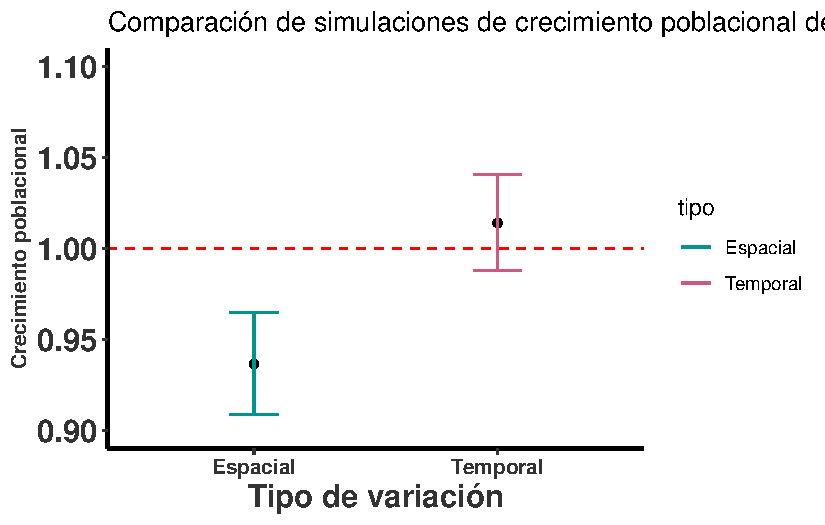
\includegraphics[keepaspectratio]{115-Metodos_de_simulaciones_files/figure-pdf/sim18-1.pdf}}

\begin{center}\rule{0.5\linewidth}{0.5pt}\end{center}

\section{Estocasticidad
demográfica}\label{estocasticidad-demogruxe1fica}

En esta sección vemos el efecto del tamaño de muestra sobre los
parámetros de la matriz de transición.

Este método usa un acercamiento Bayesiano y una distribución de
probabilidad beta para estimar los parámetros de la matriz de transición
conocida como la distribución Dirichlet múltiples para grupos discretos.
Primero vemos a que se refiere un análisis Bayesiano y la función
Dirichlet. A lo que corresponde al presenta análisis Bayesiano,
incluimos una previa al análisis, en otra palabra, se usa información
previa para incluirlos en los cálculos para estimar los parámetros, se
llaman los estimados posteriores. En nuestro caso haremos una previa con
poco peso, en otra palabra, no influirá mucho (o casi nada) en los
resultados. El concepto de previa es importante en el análisis
Bayesiano, es inherente a la filosofía de la estadística Bayesiana. Se
asume que información anterior al estudio ayuda a tomar decisión en los
cálculos los datos actuales. Como biólogos, siempre tenemos información
previa, por ejemplo, sabemos que la probabilidad de que un individuo
muera no es cero, aunque esto es evidente es una información adquirido
por nuestra experiencia previa. Ahora cual es la probabilidad exacta de
la muerte de un individuo, eso es lo que se estima en el análisis
Bayesiano tomando en cuanta tanto la información previa y la información
recolectado de un estudio.

La función Dirichlet es una expansión de una función bien básica de
probabilidad, usando una distribución beta. La función beta es una
distribución de probabilidad continua en el intervalo de {[}0,1{]} y se
usa para modelar la probabilidad de un evento binario. La función
Dirichlet es una generalización de la función beta y se usa para modelar
la probabilidad de un evento multinomial (múltiples grupos) donde la
suma de cada probabilidades es igual a 1 y las probabilidades tienen que
estar dentro del intervalo de {[}0,1{]}. En otra palabra no puede haber
valores menores de 0 o mayores de 1, incluyendo la suma de estos.

Comenzamos con lo más básico, probabilidades de dos grupos. Consideramos
un grupo de 10 individuos, si 6 de estos individuos sobreviven, cual es
la proporción que no sobreviven. La probabilidad de sobrevivir es
\(p=6/10\), entonces la probabilidad de no sobre vivir \(\hat{p}=1-p\),
porque siempre la suma de \(p + \hat{p}= 1\).

Si tenemos tres grupos, digamos, plántulas que se quedan como plántula,
que crecen a juveniles o que mueren. En este caso tenemos tres grupos
(multinomial) y la probabilidad de que un individuo de las proporciones
tiene que sumar a 1. En este caso la probabilidad de que un individuo se
queda como plántula es \(p_1=0.5\), la probabilidad de que un individuo
crece a juvenil es \(p_2=0.3\) y la probabilidad de que un individuo
muere es \(p_3=0.2\). La suma de estas probabilidades tiene que ser
igual a 1, en otra palabra \(p_1 + p_2 + p_3 = 1\).

La otra ventaja de usar la función Dirichlet es que se basa en la
distribución beta. Este es una distribución donde tanto los parámetros
como el promedio, y los intervalo de confianza son limitado a 0 y 1.
Otra manera de decir lo mismo es que no se puede tener intervalos de
confianza menos 0 o mayor de 1. Hagan el ejercicio mental de tratar de
entender un intervalo de confianza con una probabilidad de -0.10. Nota
que si uno usa una distribución normal, los intervalos de confianza
pueden ser negativos o mayores de 1, lo que no tiene sentido biológico
ni matemático en el contexto de probabilidad. De allí viene la ventaja
de usar la distribución beta para calcular los parámetros y tener claro
cual distribuciones se usa para estimar los parámetros.

\subsection{\texorpdfstring{Selecionar una población de \emph{Serapias
cordigera}}{Selecionar una población de Serapias cordigera}}\label{selecionar-una-poblaciuxf3n-de-serapias-cordigera}

Se seleciona la población A3 de \emph{Serapias cordigera} para hacer el
análisis. Esta población es una de las poblaciones afectada de forma
antropogénicas, y tiene un tamaño de muestra pequeño, lo que hace que
sea interesante para ver el efecto del tamaño de muestra en los
parámetros de la matriz de transición.

\begin{Shaded}
\begin{Highlighting}[]
\NormalTok{n }\OtherTok{\textless{}{-}} \FunctionTok{c}\NormalTok{(}\DecValTok{2}\NormalTok{, }\DecValTok{0}\NormalTok{, }\DecValTok{4}\NormalTok{, }\DecValTok{99}\NormalTok{) }\CommentTok{\# población inicial por etapa}
\FunctionTok{names}\NormalTok{(n) }\OtherTok{\textless{}{-}} \FunctionTok{c}\NormalTok{(}\StringTok{"latente"}\NormalTok{, }\StringTok{"plantula"}\NormalTok{, }\StringTok{"rosetta"}\NormalTok{, }\StringTok{"con flor"}\NormalTok{)}
\NormalTok{Serapia\_A3   }\OtherTok{\textless{}{-}} \FunctionTok{splitA}\NormalTok{(Serapia}\SpecialCharTok{$}\NormalTok{A3\_1999) }\CommentTok{\# separar la matriz A3 en sus componentes (transición y fecundidad)}
\end{Highlighting}
\end{Shaded}

\begin{center}\rule{0.5\linewidth}{0.5pt}\end{center}

\subsection{Asignar una previa a los
datos}\label{asignar-una-previa-a-los-datos}

En el siguiente paso vamos a asignar una previa a los datos. Estas
previas proviene de Tremblay, no representa la visión de los autores del
artículo. Se añade una previa también para la proporción de plantas que
fallece en cada etapa (la quita fila). Nota que es importante que la
suma de cada columna sea igual a 1. Típicamente uno debería obtener la
previa de la literatura o de un especialista en la biología de la
especie antes de la recoleccción de datos, pero en este caso no se tiene
información previa.

\begin{Shaded}
\begin{Highlighting}[]
\NormalTok{RLT\_Serapia\_previa }\OtherTok{\textless{}{-}} \FunctionTok{matrix}\NormalTok{(}\FunctionTok{c}\NormalTok{(}\FloatTok{0.5}\NormalTok{, }\FloatTok{0.1}\NormalTok{,   }\FloatTok{0.4}\NormalTok{,   }\FloatTok{0.4}\NormalTok{,}
                               \FloatTok{0.2}\NormalTok{,  }\FloatTok{0.}\NormalTok{,    }\FloatTok{0.0}\NormalTok{,   }\FloatTok{0.0}\NormalTok{,}
                               \FloatTok{0.0}\NormalTok{,  }\FloatTok{0.025}\NormalTok{, }\FloatTok{0.25}\NormalTok{,  }\FloatTok{0.3}\NormalTok{,}
                               \FloatTok{0.15}\NormalTok{,  }\FloatTok{0.05}\NormalTok{,  }\FloatTok{0.25}\NormalTok{,  }\FloatTok{0.2}\NormalTok{,}
                               \FloatTok{0.05}\NormalTok{,  }\FloatTok{0.025}\NormalTok{, }\FloatTok{0.1}\NormalTok{,   }\FloatTok{0.1}\NormalTok{), }
                       \AttributeTok{byrow =} \ConstantTok{TRUE}\NormalTok{, }\AttributeTok{nrow =} \DecValTok{5}\NormalTok{, }\AttributeTok{ncol =} \DecValTok{4}\NormalTok{)}
\end{Highlighting}
\end{Shaded}

\begin{center}\rule{0.5\linewidth}{0.5pt}\end{center}

\subsection{Obtener los intervalos de confianza (IC) para entradas de
matriz
individuales}\label{obtener-los-intervalos-de-confianza-ic-para-entradas-de-matriz-individuales}

La distribución posterior marginal de un elemento en un multinómio es
una distribución beta, y usamos esto para obtener intervalos creíbles en
nuestro tasas de transición. Podemos usar el tipo de retorno TN para
obtener los parámetros de el multinomio deseado.

Nota que:

\begin{itemize}
\tightlist
\item
  TF tiene que ser una matriz divido entre la transición y de fecundidad
  (matT + matF),
\item
  N es el tamaño de muestra de cada etapa de la vida,
\item
  P es la previa de la matriz de transición,
\item
  priorweight es el peso de la previo (en este caso estamos dando muy
  poca importancia a la previa, como si fuese una décima de un
  individuo), lo que resulta en que los datos del campo domina el
  análisis.
\item
  Regresa el posterior de la matriz de transición. Eso quiere decir que
  calcula los parámetros de la distribución beta para cada elemento de
  la matriz de transición tomando en cuenta tanto los valores de la
  matriz \textbf{TF} y la previa \textbf{P}.
\end{itemize}

En el script vemos los intervalos de confianza de la matriz de
transición de \emph{Serapias cordigera} en 1999 para la población A3.

Lo más dramático de ese primer análisis que que los intervalos de
credibilidad son bien grandes, casi todos los intervalos de credibilidad
\textbf{lcl} y \textbf{ucl} de muy cerca de cero a valores muy grande.
Esto sugiere que hay mucha incertidumbre en los datos. Este resultado es
esperado, porque la muestra es muy pequeña, solamente 2 individuos
fueron muestreado en el campo de esta etapa.

\begin{Shaded}
\begin{Highlighting}[]
\NormalTok{TN }\OtherTok{\textless{}{-}} \FunctionTok{fill\_transitions}\NormalTok{(Serapia\_A3, }\AttributeTok{N=}\NormalTok{n, }\AttributeTok{P =}\NormalTok{ RLT\_Serapia\_previa, }\AttributeTok{priorweight =}\NormalTok{ .}\DecValTok{01}\NormalTok{, }\AttributeTok{returnType =} \StringTok{"TN"}\NormalTok{)}
\NormalTok{a }\OtherTok{\textless{}{-}}\NormalTok{ TN[,}\DecValTok{1}\NormalTok{] }\CommentTok{\# cambie 1 a 2, 3 etc para obtener la distribución beta marginal de cada columna, el valor representa la columna. }
\NormalTok{b }\OtherTok{\textless{}{-}} \FunctionTok{sum}\NormalTok{(TN[,}\DecValTok{1}\NormalTok{]) }\SpecialCharTok{{-}}\NormalTok{ TN[,}\DecValTok{1}\NormalTok{]}\CommentTok{\# cambie 1 a 2, 3 etc para obtener la distribución beta marginal de cada columna. }
\NormalTok{p }\OtherTok{\textless{}{-}}\NormalTok{ a }\SpecialCharTok{/}\NormalTok{ (a }\SpecialCharTok{+}\NormalTok{ b)}
\NormalTok{lcl }\OtherTok{\textless{}{-}} \FunctionTok{qbeta}\NormalTok{(}\FloatTok{0.025}\NormalTok{, a, b)}
\NormalTok{ucl }\OtherTok{\textless{}{-}} \FunctionTok{qbeta}\NormalTok{(}\FloatTok{0.975}\NormalTok{, a, b)}
\NormalTok{A3}\OtherTok{=}\NormalTok{knitr}\SpecialCharTok{::}\FunctionTok{kable}\NormalTok{(}\FunctionTok{sprintf}\NormalTok{(}\StringTok{"\%.3f, \%.3f, \%.3f"}\NormalTok{, p, lcl, ucl))}

\NormalTok{A3df\_lat}\OtherTok{=}\FunctionTok{round}\NormalTok{(}\FunctionTok{data.frame}\NormalTok{(p, lcl, ucl), }\AttributeTok{digits=}\DecValTok{3}\NormalTok{)}
\NormalTok{A3df\_lat}\SpecialCharTok{$}\NormalTok{etapa\_futura }\OtherTok{\textless{}{-}} \FunctionTok{c}\NormalTok{(}\StringTok{"latente"}\NormalTok{, }\StringTok{"plantula"}\NormalTok{, }\StringTok{"rosetta"}\NormalTok{, }\StringTok{"con flor"}\NormalTok{, }\StringTok{"fallece"}\NormalTok{)}
\NormalTok{A3df\_lat}
\end{Highlighting}
\end{Shaded}

\begin{verbatim}
      p   lcl   ucl etapa_futura
1 0.544 0.038 0.984      latente
2 0.149 0.000 0.735     plantula
3 0.000 0.000 0.000      rosetta
4 0.241 0.000 0.844     con flor
5 0.066 0.000 0.544      fallece
\end{verbatim}

Ahora vemos que pasa con la etapa que tenemos más datos, los adultos con
flores. En este caso vemos que los intervalos de credibilidad son más
pequeños, pero todavía son grandes, ya que el tamaño de muestra es de 99
para esta etapa.

\begin{Shaded}
\begin{Highlighting}[]
\NormalTok{TN }\OtherTok{\textless{}{-}} \FunctionTok{fill\_transitions}\NormalTok{(Serapia\_A3, }\AttributeTok{N=}\NormalTok{n, }\AttributeTok{P =}\NormalTok{ RLT\_Serapia\_previa, }\AttributeTok{priorweight =} \FloatTok{0.01}\NormalTok{, }\AttributeTok{returnType =} \StringTok{"TN"}\NormalTok{)}
\NormalTok{a }\OtherTok{\textless{}{-}}\NormalTok{ TN[,}\DecValTok{4}\NormalTok{] }\CommentTok{\# cambie 1 a 2, 3 etc para obter la distribución beta marginal de cada columna. }
\NormalTok{b }\OtherTok{\textless{}{-}} \FunctionTok{sum}\NormalTok{(TN[,}\DecValTok{4}\NormalTok{]) }\SpecialCharTok{{-}}\NormalTok{ TN[,}\DecValTok{4}\NormalTok{]}\CommentTok{\# cambie 1 a 2, 3 etc para obter la distribución beta marginal de cada columna. }
\NormalTok{p }\OtherTok{\textless{}{-}}\NormalTok{ a }\SpecialCharTok{/}\NormalTok{ (a }\SpecialCharTok{+}\NormalTok{ b)}
\NormalTok{lcl }\OtherTok{\textless{}{-}} \FunctionTok{qbeta}\NormalTok{(}\FloatTok{0.025}\NormalTok{, a, b)}
\NormalTok{ucl }\OtherTok{\textless{}{-}} \FunctionTok{qbeta}\NormalTok{(}\FloatTok{0.975}\NormalTok{, a, b)}
\NormalTok{ A3}\OtherTok{=}\NormalTok{knitr}\SpecialCharTok{::}\FunctionTok{kable}\NormalTok{(}\FunctionTok{sprintf}\NormalTok{(}\StringTok{"\%.3f, \%.3f, \%.3f"}\NormalTok{, p, lcl, ucl))}

\NormalTok{A3df}\OtherTok{=}\FunctionTok{round}\NormalTok{(}\FunctionTok{data.frame}\NormalTok{(p, lcl, ucl), }\AttributeTok{digits=}\DecValTok{3}\NormalTok{)}
\NormalTok{A3df}\SpecialCharTok{$}\NormalTok{etapa\_futura }\OtherTok{\textless{}{-}} \FunctionTok{c}\NormalTok{(}\StringTok{"latente"}\NormalTok{, }\StringTok{"plantula"}\NormalTok{, }\StringTok{"rosetta"}\NormalTok{, }\StringTok{"con flor"}\NormalTok{, }\StringTok{"fallece"}\NormalTok{)}
\NormalTok{A3df}
\end{Highlighting}
\end{Shaded}

\begin{verbatim}
      p   lcl   ucl etapa_futura
1 0.004 0.000 0.022      latente
2 0.000 0.000 0.000     plantula
3 0.287 0.203 0.379      rosetta
4 0.102 0.051 0.168     con flor
5 0.607 0.510 0.700      fallece
\end{verbatim}

\subsection{Impacto de tamaño de muestra en los intervalos de
credibilidad}\label{impacto-de-tamauxf1o-de-muestra-en-los-intervalos-de-credibilidad}

\begin{tcolorbox}[enhanced jigsaw, arc=.35mm, bottomrule=.15mm, bottomtitle=1mm, breakable, colback=white, colbacktitle=quarto-callout-warning-color!10!white, colframe=quarto-callout-warning-color-frame, coltitle=black, left=2mm, leftrule=.75mm, opacityback=0, opacitybacktitle=0.6, rightrule=.15mm, title=\textcolor{quarto-callout-warning-color}{\faExclamationTriangle}\hspace{0.5em}{Advertencia}, titlerule=0mm, toprule=.15mm, toptitle=1mm]

\textbf{La simulación no inventa información que no está en los datos.}
Una población con sólo 2 plántulas observadas tendrá intervalos de
credibilidad muy amplios, y eso es lo correcto: refleja la verdadera
incertidumbre del muestreo. Aumentar el número de simulaciones
(\texttt{nreps}) no estrecha los intervalos --- sólo los estima con más
precisión. Para estrechar intervalos se necesitan \textbf{más datos de
campo} (más individuos marcados, más años de muestreo) o \textbf{previas
informativas más fuertes} (justificadas por conocimiento experto). El
enfoque bayesiano hace explícito este tradeoff entre datos y
conocimiento previo.

\end{tcolorbox}

Como ejercicio, vemos que tipo de intervalos si tuviésemos tamaño de
muestra de 500 individuos en la etapa de adulto. Nota que aun que los
intervalos de credibilidad son más pequeños, no se debería asumir que no
hay variación demográfica en la etapa de adulto, por procesos
estocásticos.

\begin{Shaded}
\begin{Highlighting}[]
\NormalTok{n500 }\OtherTok{\textless{}{-}} \FunctionTok{c}\NormalTok{(}\DecValTok{2}\NormalTok{, }\DecValTok{0}\NormalTok{, }\DecValTok{4}\NormalTok{, }\DecValTok{500}\NormalTok{) }\CommentTok{\# población inicial por etapa}
\NormalTok{TN }\OtherTok{\textless{}{-}} \FunctionTok{fill\_transitions}\NormalTok{(Serapia\_A3, }\AttributeTok{N=}\NormalTok{n500, }\AttributeTok{P =}\NormalTok{ RLT\_Serapia\_previa, }\AttributeTok{priorweight =} \FloatTok{0.01}\NormalTok{, }\AttributeTok{returnType =} \StringTok{"TN"}\NormalTok{)}
\NormalTok{a500 }\OtherTok{\textless{}{-}}\NormalTok{ TN[,}\DecValTok{4}\NormalTok{] }\CommentTok{\# cambie 1 a 2, 3 o 4 etc. para obtener la distribución beta marginal de cada columna (etapas).}
\NormalTok{b500 }\OtherTok{\textless{}{-}} \FunctionTok{sum}\NormalTok{(TN[,}\DecValTok{4}\NormalTok{]) }\SpecialCharTok{{-}}\NormalTok{ TN[,}\DecValTok{4}\NormalTok{]}\CommentTok{\# cambie 1 a 2, 3 etc. para obtener la distribución beta marginal de cada columna.}
\NormalTok{p500 }\OtherTok{\textless{}{-}}\NormalTok{ a500 }\SpecialCharTok{/}\NormalTok{ (a500 }\SpecialCharTok{+}\NormalTok{ b500)}
\NormalTok{lcl }\OtherTok{\textless{}{-}} \FunctionTok{qbeta}\NormalTok{(}\FloatTok{0.025}\NormalTok{, a500, b500)}
\NormalTok{ucl }\OtherTok{\textless{}{-}} \FunctionTok{qbeta}\NormalTok{(}\FloatTok{0.975}\NormalTok{, a500, b500)}
\NormalTok{ A3}\OtherTok{=}\NormalTok{knitr}\SpecialCharTok{::}\FunctionTok{kable}\NormalTok{(}\FunctionTok{sprintf}\NormalTok{(}\StringTok{"\%.3f, \%.3f, \%.3f"}\NormalTok{, p, lcl, ucl))}

\NormalTok{A3df}\OtherTok{=}\FunctionTok{round}\NormalTok{(}\FunctionTok{data.frame}\NormalTok{(p, lcl, ucl), }\AttributeTok{digits=}\DecValTok{3}\NormalTok{)}
\NormalTok{A3df}\SpecialCharTok{$}\NormalTok{etapa\_futura }\OtherTok{\textless{}{-}} \FunctionTok{c}\NormalTok{(}\StringTok{"latente"}\NormalTok{, }\StringTok{"plantula"}\NormalTok{, }\StringTok{"rosetta"}\NormalTok{, }\StringTok{"con flor"}\NormalTok{, }\StringTok{"fallece"}\NormalTok{)}
\NormalTok{A3df}
\end{Highlighting}
\end{Shaded}

\begin{verbatim}
      p   lcl   ucl etapa_futura
1 0.004 0.000 0.011      latente
2 0.000 0.000 0.000     plantula
3 0.287 0.249 0.327      rosetta
4 0.102 0.077 0.130     con flor
5 0.607 0.564 0.649      fallece
\end{verbatim}

\subsection{Visualización de la distribución
beta}\label{visualizaciuxf3n-de-la-distribuciuxf3n-beta}

Ahora vemos cómo se distribuye una distribución beta. Usamos los datos
de la etapa de adulto con flores con 99 individuos. Se observa que
ninguna de las transiciones o estasis tiene una distribución normal. La
distribución que demuestra bien este patrón es la de los adultos con
flores que pasan a latente. La línea roja vertical representa el
promedio, es decir, el valor en la matriz de transición.

\begin{Shaded}
\begin{Highlighting}[]
\NormalTok{a }\CommentTok{\# los valores del shape alpha }
\end{Highlighting}
\end{Shaded}

\begin{verbatim}
[1]  0.396  0.000 28.710 10.197 60.687
\end{verbatim}

\begin{Shaded}
\begin{Highlighting}[]
\NormalTok{b }\CommentTok{\# los valores del shape beta}
\end{Highlighting}
\end{Shaded}

\begin{verbatim}
[1] 99.594 99.990 71.280 89.793 39.303
\end{verbatim}

\begin{Shaded}
\begin{Highlighting}[]
\CommentTok{\# Función para visualizar la distribution beta}
\NormalTok{plot\_beta }\OtherTok{\textless{}{-}} \ControlFlowTok{function}\NormalTok{(alpha, beta) \{}
\NormalTok{  x }\OtherTok{\textless{}{-}} \FunctionTok{seq}\NormalTok{(}\DecValTok{0}\NormalTok{, }\DecValTok{1}\NormalTok{, }\AttributeTok{length.out =} \DecValTok{100}\NormalTok{)}
\NormalTok{  y }\OtherTok{\textless{}{-}} \FunctionTok{dbeta}\NormalTok{(x, alpha, beta)}
\NormalTok{  data }\OtherTok{\textless{}{-}} \FunctionTok{data.frame}\NormalTok{(}\AttributeTok{x =}\NormalTok{ x, }\AttributeTok{y =}\NormalTok{ y)}
  \FunctionTok{ggplot}\NormalTok{(data, }\FunctionTok{aes}\NormalTok{(x, y)) }\SpecialCharTok{+}
    \FunctionTok{geom\_line}\NormalTok{()}
\NormalTok{\}}

\CommentTok{\# Distirbuciones beta}
\NormalTok{Latentes}\OtherTok{=}\FunctionTok{plot\_beta}\NormalTok{(}\FloatTok{0.396}\NormalTok{, }\FloatTok{99.594}\NormalTok{)}\SpecialCharTok{+}
  \FunctionTok{xlim}\NormalTok{(}\DecValTok{0}\NormalTok{, .}\DecValTok{1}\NormalTok{)}\SpecialCharTok{+}
    \FunctionTok{labs}\NormalTok{(}\AttributeTok{title =} \FunctionTok{paste}\NormalTok{(}\StringTok{"Distribución de latentes }\SpecialCharTok{\textbackslash{}n}\StringTok{ (alpha ="}\NormalTok{, }\FloatTok{0.396}\NormalTok{, }\StringTok{", beta ="}\NormalTok{, }\FloatTok{99.594}\NormalTok{, }\StringTok{")"}\NormalTok{),}
         \AttributeTok{x =} \StringTok{"Probabilidad"}\NormalTok{, }\AttributeTok{y =} \StringTok{"Densidad"}\NormalTok{)}\SpecialCharTok{+}
    \FunctionTok{theme}\NormalTok{(}\AttributeTok{text =} \FunctionTok{element\_text}\NormalTok{(}\AttributeTok{size =} \DecValTok{6}\NormalTok{))}\SpecialCharTok{+}
  \FunctionTok{geom\_vline}\NormalTok{(}\AttributeTok{xintercept =} \FloatTok{0.004}\NormalTok{, }\AttributeTok{linetype =} \StringTok{"dashed"}\NormalTok{, }\AttributeTok{color =} \StringTok{"\#009392"}\NormalTok{)}

\NormalTok{Plantulas}\OtherTok{=}\FunctionTok{plot\_beta}\NormalTok{(}\FloatTok{0.000}\NormalTok{, }\FloatTok{99.990}\NormalTok{)}\SpecialCharTok{+}
  \FunctionTok{xlim}\NormalTok{(}\DecValTok{0}\NormalTok{, .}\DecValTok{025}\NormalTok{)}\SpecialCharTok{+}\FunctionTok{ylim}\NormalTok{(}\DecValTok{0}\NormalTok{, .}\DecValTok{05}\NormalTok{)}\SpecialCharTok{+}
    \FunctionTok{labs}\NormalTok{(}\AttributeTok{title =} \FunctionTok{paste}\NormalTok{(}\StringTok{"Distribución de plántulas }\SpecialCharTok{\textbackslash{}n}\StringTok{ (alpha ="}\NormalTok{, }\FloatTok{0.000}\NormalTok{, }\StringTok{", beta ="}\NormalTok{, }\FloatTok{99.90}\NormalTok{, }\StringTok{")"}\NormalTok{),}
         \AttributeTok{x =} \StringTok{"probabilidad"}\NormalTok{, }\AttributeTok{y =} \StringTok{"Densidad"}\NormalTok{)}\SpecialCharTok{+}
    \FunctionTok{theme}\NormalTok{(}\AttributeTok{text =} \FunctionTok{element\_text}\NormalTok{(}\AttributeTok{size =} \DecValTok{6}\NormalTok{))}\SpecialCharTok{+}
  \FunctionTok{geom\_vline}\NormalTok{(}\AttributeTok{xintercept =} \FloatTok{0.000}\NormalTok{, }\AttributeTok{linetype =} \StringTok{"dashed"}\NormalTok{, }\AttributeTok{color =} \StringTok{"\#009392"}\NormalTok{)}

\NormalTok{Rosetta}\OtherTok{=}\FunctionTok{plot\_beta}\NormalTok{(}\FloatTok{28.710}\NormalTok{, }\FloatTok{71.280}\NormalTok{)}\SpecialCharTok{+}
  \FunctionTok{xlim}\NormalTok{(}\DecValTok{0}\NormalTok{, .}\DecValTok{5}\NormalTok{)}\SpecialCharTok{+}
    \FunctionTok{labs}\NormalTok{(}\AttributeTok{title =} \FunctionTok{paste}\NormalTok{(}\StringTok{"Distribución de rosettas }\SpecialCharTok{\textbackslash{}n}\StringTok{ (alpha ="}\NormalTok{, }\FloatTok{28.710}\NormalTok{, }\StringTok{", beta ="}\NormalTok{, }\FloatTok{71.280}\NormalTok{, }\StringTok{")"}\NormalTok{),}
         \AttributeTok{x =} \StringTok{"probabilidad"}\NormalTok{, }\AttributeTok{y =} \StringTok{"Densidad"}\NormalTok{)}\SpecialCharTok{+}
    \FunctionTok{theme}\NormalTok{(}\AttributeTok{text =} \FunctionTok{element\_text}\NormalTok{(}\AttributeTok{size =} \DecValTok{6}\NormalTok{))}\SpecialCharTok{+}
  \FunctionTok{geom\_vline}\NormalTok{(}\AttributeTok{xintercept =} \FloatTok{0.287}\NormalTok{, }\AttributeTok{linetype =} \StringTok{"dashed"}\NormalTok{, }\AttributeTok{color =} \StringTok{"\#009392"}\NormalTok{)}

\NormalTok{Adultos}\OtherTok{=}\FunctionTok{plot\_beta}\NormalTok{(}\FloatTok{10.197}\NormalTok{, }\FloatTok{89.793}\NormalTok{)}\SpecialCharTok{+}
  \FunctionTok{xlim}\NormalTok{(}\DecValTok{0}\NormalTok{, .}\DecValTok{27}\NormalTok{)}\SpecialCharTok{+}
    \FunctionTok{labs}\NormalTok{(}\AttributeTok{title =} \FunctionTok{paste}\NormalTok{(}\StringTok{"Distribución de Ind. con flores }\SpecialCharTok{\textbackslash{}n}\StringTok{ (alpha ="}\NormalTok{, }\FloatTok{10.197}\NormalTok{, }\StringTok{", beta ="}\NormalTok{, }\FloatTok{89.793}\NormalTok{, }\StringTok{")"}\NormalTok{),}
         \AttributeTok{x =} \StringTok{"probabilidad"}\NormalTok{, }\AttributeTok{y =} \StringTok{"Densidad"}\NormalTok{)}\SpecialCharTok{+}
    \FunctionTok{theme}\NormalTok{(}\AttributeTok{text =} \FunctionTok{element\_text}\NormalTok{(}\AttributeTok{size =} \DecValTok{6}\NormalTok{))}\SpecialCharTok{+}
  \FunctionTok{geom\_vline}\NormalTok{(}\AttributeTok{xintercept =} \FloatTok{0.102}\NormalTok{, }\AttributeTok{linetype =} \StringTok{"dashed"}\NormalTok{, }\AttributeTok{color =} \StringTok{"\#009392"}\NormalTok{)}

\NormalTok{Fallecidos}\OtherTok{=}\FunctionTok{plot\_beta}\NormalTok{(}\FloatTok{60.687}\NormalTok{, }\FloatTok{39.303}\NormalTok{)}\SpecialCharTok{+}
  \FunctionTok{xlim}\NormalTok{(.}\DecValTok{40}\NormalTok{, .}\DecValTok{8}\NormalTok{)}\SpecialCharTok{+}
    \FunctionTok{labs}\NormalTok{(}\AttributeTok{title =} \FunctionTok{paste}\NormalTok{(}\StringTok{"Distribución de fallecidos }\SpecialCharTok{\textbackslash{}n}\StringTok{ (alpha ="}\NormalTok{, }\FloatTok{60.687}\NormalTok{, }\StringTok{", beta ="}\NormalTok{, }\FloatTok{39.303}\NormalTok{, }\StringTok{")"}\NormalTok{),}
         \AttributeTok{x =} \StringTok{"probabilidad"}\NormalTok{, }\AttributeTok{y =} \StringTok{"Densidad"}\NormalTok{)}\SpecialCharTok{+}
    \FunctionTok{theme}\NormalTok{(}\AttributeTok{text =} \FunctionTok{element\_text}\NormalTok{(}\AttributeTok{size =} \DecValTok{6}\NormalTok{))}\SpecialCharTok{+}
  \FunctionTok{geom\_vline}\NormalTok{(}\AttributeTok{xintercept =} \FloatTok{0.607}\NormalTok{, }\AttributeTok{linetype =} \StringTok{"dashed"}\NormalTok{, }\AttributeTok{color =} \StringTok{"\#009392"}\NormalTok{)}

\FunctionTok{ggarrange}\NormalTok{(Latentes, Plantulas, Rosetta, Adultos, Fallecidos, }\AttributeTok{ncol=}\DecValTok{3}\NormalTok{, }\AttributeTok{nrow=}\DecValTok{2}\NormalTok{)}
\end{Highlighting}
\end{Shaded}

\pandocbounded{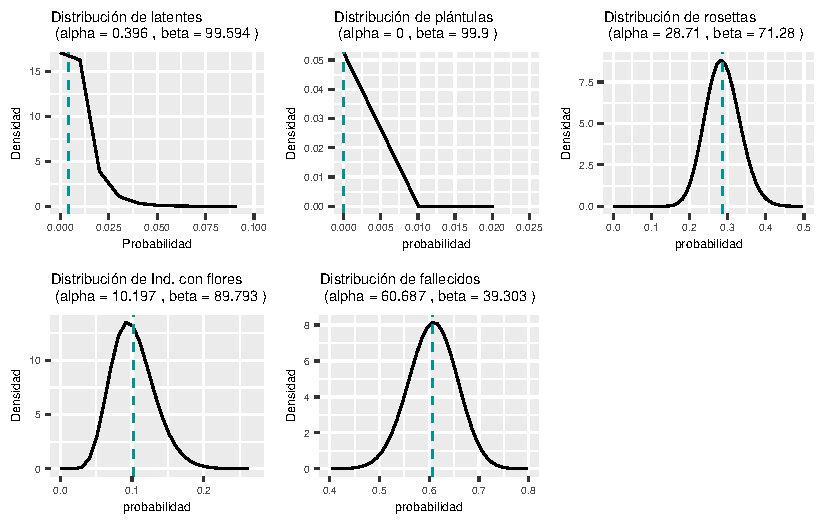
\includegraphics[keepaspectratio]{115-Metodos_de_simulaciones_files/figure-pdf/sim25-1.pdf}}

\begin{Shaded}
\begin{Highlighting}[]
\FunctionTok{ggsave}\NormalTok{(}\StringTok{"mi\_gragico.tiff"}\NormalTok{)}
\end{Highlighting}
\end{Shaded}

\begin{center}\rule{0.5\linewidth}{0.5pt}\end{center}

\section{Ventaja de usar
simulaciones}\label{ventaja-de-usar-simulaciones}

La primera ventaja de usar métodos de análisis por simulaciones es que
se puede calcula intervalos de confianza. Si los intervalos de confianza
de lambda solapa el uno (1) (o solapa el 0 para \(log\lambda\)) entonces
no hay evidencia de que el crecimiento poblacional es diferente de
estable.

La segunda ventaja de usar simulaciones es que hay que recordar que los
análisis están basado en datos limitados y que si hubiese más o menos
datos para estimar los elementos de la matriz la parámetros de la matriz
pudiese ser diferentes. Entonces hay un componente de incertidumbre en
los estimados de los parámetros de la matriz, los valores de promedio no
recolectan esa variación entre individuos, tiempo y espacio.

La incertidumbre por causas intrínsecas (los individuos, la genética, el
tamaño de muestra) y extrínsecas (hábitat, tiempo, variación en
polinizadores, herbívoros, etc.) se evalúa usando análisis de variación
espacial, temporal y demográfica. La incertidumbre en los parámetros de
la matriz de transición se puede cuantificar con intervalos de confianza
o con el intervalo de credibilidad (concepto bayesiano). Es de suma
importancia que se evalúe la incertidumbre en los parámetros de la
matriz de transición para tener un mejor entendimiento de dónde proviene
la variación y la incertidumbre en el crecimiento poblacional de una
especie, y saber si hay suficiente evidencia para tener confianza en si
la especie está en declive, crece o se mantiene estable.

\bookmarksetup{startatroot}

\chapter{COMPADRE y Orquídeas}\label{Compadre}

\emph{Por: Raymond L. Tremblay}

\begin{tcolorbox}[enhanced jigsaw, arc=.35mm, bottomrule=.15mm, bottomtitle=1mm, breakable, colback=white, colbacktitle=quarto-callout-note-color!10!white, colframe=quarto-callout-note-color-frame, coltitle=black, left=2mm, leftrule=.75mm, opacityback=0, opacitybacktitle=0.6, rightrule=.15mm, title=\textcolor{quarto-callout-note-color}{\faInfo}\hspace{0.5em}{Qué es este capítulo}, titlerule=0mm, toprule=.15mm, toptitle=1mm]

Este capítulo es una \textbf{guía práctica de uso del paquete
\texttt{Rcompadre}}. No introduce conceptos nuevos sobre dinámica
poblacional ---para eso están los capítulos del 4 al 16---, sino que
enseña a manejar la base COMPADRE con confianza: cómo descargarla,
filtrarla, validar las matrices, extraer las submatrices U/F/C, y
conectar los datos con los análisis del resto del libro. El paquete
\texttt{Rcompadre} no es trivial: tiene su propia clase de objetos
(\texttt{CompadreDB}), funciones con nombres similares pero
comportamientos distintos, y trampas que cuestan tiempo si uno las
descubre por prueba y error. Este capítulo busca acortar esa curva de
aprendizaje.

\end{tcolorbox}

Los datos demográficos comparables son la base para analizar la dinámica
de poblaciones de orquídeas a través de especies, regiones y contextos
ambientales. Este capítulo presenta el conjunto de datos de orquídeas
derivado de la base COMPADRE y describe su organización para usarlos en
los modelos y análisis del libro.

\section{Alcance y organización de los datos demográficos de
orquídeas}\label{alcance-y-organizaciuxf3n-de-los-datos-demogruxe1ficos-de-orquuxeddeas}

El conjunto de datos de orquídeas reúne matrices de proyección
poblacional y metadatos asociados (especie, ubicación, periodo de
muestreo, tipo de hábitat y notas metodológicas) que permiten comparar
la dinámica demográfica entre poblaciones y especies. La estructura de
los datos facilita la construcción de matrices \textbf{U}, \textbf{F} y
\textbf{C}, el cálculo de la tasa de crecimiento poblacional (λ) y la
implementación de análisis de sensibilidad, elasticidad y LTRE, así como
simulaciones bajo distintos escenarios.

En esta sección se describe cómo están organizadas las tablas
principales ---una tabla de \textbf{matrices} y una tabla de
\textbf{metadatos}---, las claves que las conectan
(especies/poblaciones/estudios) y las precauciones habituales al
trabajar con información heterogénea (año de referencia, definición de
estadios, unidades de medida y supuestos de reclutamiento). También se
presenta una vista general de la cobertura taxonómica y geográfica del
conjunto, con el fin de contextualizar cualquier patrón observado.

A diferencia de los capítulos analíticos, este capítulo no introduce
nuevos métodos; su objetivo es proporcionar un recurso de datos
\textbf{listo para analizar} que permita replicar ejemplos, comparar
patrones demográficos entre orquídeas y vincular resultados con
decisiones de manejo y conservación. La documentación clara de la
estructura y las variables garantiza que los análisis posteriores sean
reproducibles e interpretables en el marco del libro.

\section{Estructura del conjunto de datos y carga en el
entorno}\label{estructura-del-conjunto-de-datos-y-carga-en-el-entorno}

A continuación se describen las tablas principales y se muestra cómo
cargar y verificar el conjunto de datos en el entorno de trabajo.

Los datos aquí descritos se integran directamente en la descomposición
en matrices U, F y C y en el cálculo de crecimiento poblacional. La
comparación de la importancia relativa de transiciones puede realizarse
mediante elasticidad poblacional y la explicación de diferencias
observadas entre poblaciones mediante LTRE. Para explorar escenarios
alternativos, puede utilizarse el capítulo de métodos de simulaciones.

\subsection{Cobertura y limitaciones}\label{cobertura-y-limitaciones}

La cobertura taxonómica y espacial es heterogénea entre especies y
poblaciones. Algunas series temporales son cortas o presentan años sin
muestreo; en estos casos se debe documentar cualquier decisión de
imputación o agregación. Las definiciones de estadios y los supuestos de
reclutamiento pueden variar entre estudios; por ello, al comparar
poblaciones conviene revisar la documentación asociada y mantener
criterios consistentes de armonización.

\begin{tcolorbox}[enhanced jigsaw, arc=.35mm, bottomrule=.15mm, bottomtitle=1mm, breakable, colback=white, colbacktitle=quarto-callout-warning-color!10!white, colframe=quarto-callout-warning-color-frame, coltitle=black, left=2mm, leftrule=.75mm, opacityback=0, opacitybacktitle=0.6, rightrule=.15mm, title=\textcolor{quarto-callout-warning-color}{\faExclamationTriangle}\hspace{0.5em}{Advertencia}, titlerule=0mm, toprule=.15mm, toptitle=1mm]

\textbf{COMPADRE agrega estudios diversos --- la armonización es
responsabilidad del usuario.} Las matrices de la base provienen de
estudios con definiciones de estadios distintas, periodos de muestreo
variables (mensual a multianual) y supuestos de reclutamiento
diferentes. La columna \texttt{MatrixComposite} indica si una matriz es
individual, promedio o \emph{pooled}. Antes de comparar matrices entre
estudios, conviene revisar:

\begin{itemize}
\tightlist
\item
  \texttt{MatrixDimension}: ¿el número de estadios es comparable?
\item
  \texttt{StudyDuration} y \texttt{Periodicity}: ¿los pasos de tiempo
  son iguales?
\item
  \texttt{MatrixCriteriaSize} / \texttt{MatrixCriteriaAge} /
  \texttt{MatrixCriteriaOntogeny}: ¿los criterios de clasificación son
  compatibles?
\end{itemize}

Sin esta armonización, las ``comparaciones entre especies'' pueden ser
artefactos del diseño metodológico, no diferencias biológicas reales.

\end{tcolorbox}

\subsubsection{Librerías de R requeridas para el siguiente
módulo}\label{libreruxedas-de-r-requeridas-para-el-siguiente-muxf3dulo-13}

\begin{Shaded}
\begin{Highlighting}[]
\FunctionTok{library}\NormalTok{(Rcompadre) }\CommentTok{\# Paquete para trabajar con la base de datos de COMPADRE y COMADRE}
\FunctionTok{library}\NormalTok{(tidyverse) }\CommentTok{\# Paquete para activar múltiples paquetes}
\FunctionTok{library}\NormalTok{(flextable) }\CommentTok{\# Paquete para formatear tablas}

\FunctionTok{library}\NormalTok{(broom)}
\FunctionTok{library}\NormalTok{(ggdist)}
\FunctionTok{library}\NormalTok{(distributional)}
\FunctionTok{library}\NormalTok{(leaflet)}
\FunctionTok{library}\NormalTok{(Rage) }\CommentTok{\# función para calcular el largo de vida esperada entre otras}
\FunctionTok{library}\NormalTok{(car)}
\FunctionTok{library}\NormalTok{(popdemo)}
\end{Highlighting}
\end{Shaded}

Uno de los esfuerzos más grandes para compilar el conocimiento actual
sobre la ecología de poblaciones es la creación y mantenimiento de las
bases de datos de COMPADRE y COMADRE. COMPADRE es una base de datos de
matrices de proyección poblacional de \textbf{plantas}; COMADRE es la
base correspondiente para \textbf{animales}. En este capítulo se
presenta una introducción a COMPADRE y algunas de las funciones del
paquete \texttt{Rcompadre}. En el próximo capítulo se presentan
funciones del paquete \texttt{Rage}. La información aquí no sustituye la
documentación oficial en la \href{https://compadre-db.org/}{página web
de COMPADRE} ni los tutoriales en la
\href{https://compadre-db.org/Education}{sección Education}.

El valor de las bases de datos reside en tener en un mismo sitio una
gran cantidad de información ~organizada de manera uniforme y accesible,
además de que su formato permite utilizarla directamente en diferentes
análisis. En el caso de COMPADRE y COMADRE, la información está
organizada en matrices de transición de estados de poblaciones (MPP) que
se pueden usar para evaluar la dinámica de poblaciones de plantas y
animales y con múltiples variables, tal como sus coordenadas
geográficas, el tipo de hábitat, la temporalidad de los datos, la fuente
de la información, entre otros.

En este capítulo se aprenderá a utilizar COMPADRE para evaluar la
dinámica de poblaciones de orquídeas, extrayendo diferentes tipos de
datos para responder preguntas específicas.

\begin{tcolorbox}[enhanced jigsaw, arc=.35mm, bottomrule=.15mm, bottomtitle=1mm, breakable, colback=white, colbacktitle=quarto-callout-tip-color!10!white, colframe=quarto-callout-tip-color-frame, coltitle=black, left=2mm, leftrule=.75mm, opacityback=0, opacitybacktitle=0.6, rightrule=.15mm, title=\textcolor{quarto-callout-tip-color}{\faLightbulb}\hspace{0.5em}{Recomendación}, titlerule=0mm, toprule=.15mm, toptitle=1mm]

\textbf{Flujo de trabajo recomendado con COMPADRE.}

\begin{enumerate}
\def\labelenumi{\arabic{enumi}.}
\tightlist
\item
  \textbf{Cargar} la base completa una sola vez (\texttt{compadre}).
\item
  \textbf{Filtrar} a la familia, género o especie de interés
  (\texttt{filter()}).
\item
  \textbf{Validar} con \texttt{cdb\_flag()} para detectar problemas
  (NAs, no ergodicidad, etc.).
\item
  \textbf{Extraer} las matrices (\texttt{matU()}, \texttt{matF()},
  \texttt{matC()}, \texttt{matA()}).
\item
  \textbf{Analizar} con \texttt{popbio}/\texttt{popdemo}/\texttt{Rage}
  según la pregunta.
\end{enumerate}

Este capítulo cubre los pasos 1--4. El paso 5 se desarrolla en los
capítulos analíticos (elasticidad, LTRE, simulaciones, funciones de
transferencia).

\end{tcolorbox}

\begin{tcolorbox}[enhanced jigsaw, arc=.35mm, bottomrule=.15mm, bottomtitle=1mm, breakable, colback=white, colbacktitle=quarto-callout-tip-color!10!white, colframe=quarto-callout-tip-color-frame, coltitle=black, left=2mm, leftrule=.75mm, opacityback=0, opacitybacktitle=0.6, rightrule=.15mm, title=\textcolor{quarto-callout-tip-color}{\faLightbulb}\hspace{0.5em}{¿Qué función de \texttt{Rcompadre} necesito? --- Árbol de decisión}, titlerule=0mm, toprule=.15mm, toptitle=1mm]

{\def\LTcaptype{none} % do not increment counter
\begin{longtable}[]{@{}
  >{\raggedright\arraybackslash}p{(\linewidth - 2\tabcolsep) * \real{0.5000}}
  >{\raggedright\arraybackslash}p{(\linewidth - 2\tabcolsep) * \real{0.5000}}@{}}
\toprule\noalign{}
\begin{minipage}[b]{\linewidth}\raggedright
Si quiero\ldots{}
\end{minipage} & \begin{minipage}[b]{\linewidth}\raggedright
Use
\end{minipage} \\
\midrule\noalign{}
\endhead
\bottomrule\noalign{}
\endlastfoot
Bajar la base completa por primera vez &
\texttt{cdb\_fetch("compadre")} \\
Ver los metadatos (especie, año, ubicación, etc.) &
\texttt{cdb\_metadata(x)} \\
Filtrar a una familia & \texttt{subset(x,\ Family\ ==\ "Orchidaceae")}
\emph{o}
\texttt{x\ \%\textgreater{}\%\ filter(Family\ ==\ "Orchidaceae")} \\
Filtrar a una especie &
\texttt{subset(x,\ SpeciesAccepted\ ==\ "Lepanthes\ caritensis")} \\
Marcar matrices con problemas (NAs, no-ergódicas, no-irreducibles) &
\texttt{cdb\_flag(x)} --- añade columnas \texttt{check\_*}, no filtra \\
Quedarme sólo con matrices ``limpias'' &
\texttt{subset(cdb\_flag(x),\ check\_NA\_A\ ==\ FALSE\ \&\ check\_ergodic\ ==\ TRUE)} \\
Extraer la matriz de transición completa A & \texttt{matA(x)} → lista de
matrices \\
Extraer las submatrices & \texttt{matU(x)}, \texttt{matF(x)},
\texttt{matC(x)} \\
Una matriz individual & \texttt{matA(x){[}{[}i{]}{]}} (la i-ésima) \\
Aplicar una función a todas las matrices &
\texttt{purrr::map\_dbl(matA(x),\ \textasciitilde{}\ popbio::lambda(.x))} \\
\end{longtable}
}

\textbf{Regla práctica.} Si no está seguro de qué función usar, casi
siempre necesita: \texttt{cdb\_fetch()} → \texttt{subset()} o
\texttt{filter()} → \texttt{cdb\_flag()} → \texttt{subset(check\_*\ )} →
\texttt{matU()} / \texttt{matF()} / \texttt{matA()}.

\end{tcolorbox}

\begin{tcolorbox}[enhanced jigsaw, arc=.35mm, bottomrule=.15mm, bottomtitle=1mm, breakable, colback=white, colbacktitle=quarto-callout-warning-color!10!white, colframe=quarto-callout-warning-color-frame, coltitle=black, left=2mm, leftrule=.75mm, opacityback=0, opacitybacktitle=0.6, rightrule=.15mm, title=\textcolor{quarto-callout-warning-color}{\faExclamationTriangle}\hspace{0.5em}{Trampas comunes con \texttt{Rcompadre}}, titlerule=0mm, toprule=.15mm, toptitle=1mm]

\begin{itemize}
\tightlist
\item
  \textbf{\texttt{subset()} no es base-R.} \texttt{Rcompadre} exporta su
  propio método \texttt{subset()} para objetos \texttt{CompadreDB}; la
  sintaxis se parece a base-R pero respeta la estructura interna del
  objeto. \textbf{No} uses \texttt{{[}{]}} para subconjuntos directos.
\item
  \textbf{\texttt{mat} ≠ \texttt{matA()}}. \texttt{mat} es una columna
  del data-frame interno; \texttt{matA()} es la función que extrae la
  matriz A de cada fila. Use siempre la función.
\item
  \textbf{\texttt{cdb\_flag()} añade columnas, no filtra}. Después de
  \texttt{cdb\_flag()} hay que filtrar manualmente con las columnas
  \texttt{check\_*} (\texttt{check\_NA\_A}, \texttt{check\_ergodic},
  \texttt{check\_irreducible}).
\item
  \textbf{\texttt{Lat} y \texttt{Lon} a veces son \texttt{character}, no
  \texttt{numeric}}. Verifíquelo con \texttt{class()} antes de mapear o
  calcular distancias; convierta con \texttt{as.numeric()} si es
  necesario.
\item
  \textbf{\texttt{MatrixComposite}} indica si una matriz fue promediada
  o agrupada (\emph{pooled}). Para análisis comparativo conviene
  quedarse con \texttt{MatrixComposite\ ==\ "Individual"} para evitar
  pseudoreplicación.
\item
  \textbf{\texttt{MatrixCriteriaSize} / \texttt{MatrixCriteriaAge} /
  \texttt{MatrixCriteriaOntogeny}} describen cómo se definieron los
  estadios. Antes de comparar matrices entre estudios, conviene
  verificar que estos criterios sean compatibles.
\end{itemize}

\end{tcolorbox}

\begin{tcolorbox}[enhanced jigsaw, arc=.35mm, bottomrule=.15mm, bottomtitle=1mm, breakable, colback=white, colbacktitle=quarto-callout-note-color!10!white, colframe=quarto-callout-note-color-frame, coltitle=black, left=2mm, leftrule=.75mm, opacityback=0, opacitybacktitle=0.6, rightrule=.15mm, title=\textcolor{quarto-callout-note-color}{\faInfo}\hspace{0.5em}{Campos de metadatos esenciales}, titlerule=0mm, toprule=.15mm, toptitle=1mm]

De los más de 50 campos en COMPADRE, estos 9 son los que usará el 95\%
del tiempo:

{\def\LTcaptype{none} % do not increment counter
\begin{longtable}[]{@{}
  >{\raggedright\arraybackslash}p{(\linewidth - 2\tabcolsep) * \real{0.5000}}
  >{\raggedright\arraybackslash}p{(\linewidth - 2\tabcolsep) * \real{0.5000}}@{}}
\toprule\noalign{}
\begin{minipage}[b]{\linewidth}\raggedright
Campo
\end{minipage} & \begin{minipage}[b]{\linewidth}\raggedright
Qué contiene
\end{minipage} \\
\midrule\noalign{}
\endhead
\bottomrule\noalign{}
\endlastfoot
\texttt{Family} & Familia taxonómica (ej. \texttt{"Orchidaceae"}) \\
\texttt{SpeciesAccepted} & Nombre científico aceptado \\
\texttt{MatrixPopulation} & Identificador de la población (varias por
especie en muchos estudios) \\
\texttt{StudyStart}/\texttt{StudyEnd} & Años de inicio y fin del
muestreo \\
\texttt{MatrixDimension} & Número de estadios en la matriz \\
\texttt{OrganismType} & ``Epiphyte'', ``Herbaceous perennial'', etc. \\
\texttt{Lat}, \texttt{Lon} & Coordenadas de la población (a menudo como
texto, ver Trampas) \\
\texttt{MatrixComposite} & ``Individual'' / ``Mean'' / ``Pooled'' ---
clave para análisis comparativos \\
\texttt{DOI\_ISBN} & Identificador del estudio original \\
\end{longtable}
}

Para la lista completa: \texttt{?Rcompadre::CompadreDB} y la
documentación oficial.

\end{tcolorbox}

\begin{center}\rule{0.5\linewidth}{0.5pt}\end{center}

\section{Acceso a los datos de
COMPADRE}\label{acceso-a-los-datos-de-compadre}

Hay tres formas de obtener la base. Las tres dejan en el entorno un
objeto llamado \texttt{compadre} que contiene todas las matrices y
metadatos.

\subsection{Opción 1 --- Descarga manual desde la página
web}\label{opciuxf3n-1-descarga-manual-desde-la-puxe1gina-web}

La forma más sencilla es descargar el archivo \texttt{.RData} desde la
página oficial: \url{https://compadre-db.org/Data/Compadre}. Al momento
de la edición de este libro la versión más reciente es la 6.28.8.0
(agosto 2025). Una vez descargado, se carga con \texttt{load()}:

\begin{Shaded}
\begin{Highlighting}[]
\FunctionTok{load}\NormalTok{(}\StringTok{"ruta/a/COMPADRE\_v.6.28.8.0.RData"}\NormalTok{)}
\end{Highlighting}
\end{Shaded}

\subsection{Opción 2 --- Descarga directa desde
R}\label{opciuxf3n-2-descarga-directa-desde-r}

El paquete \texttt{Rcompadre} incluye la función \texttt{cdb\_fetch()}
que descarga la última versión directamente desde R, sin necesidad de
descargar el archivo manualmente:

\begin{Shaded}
\begin{Highlighting}[]
\NormalTok{compadre }\OtherTok{\textless{}{-}} \FunctionTok{cdb\_fetch}\NormalTok{(}\StringTok{"compadre"}\NormalTok{)}
\end{Highlighting}
\end{Shaded}

\subsection{Opción 3 --- Archivo precompilado de este
libro}\label{opciuxf3n-3-archivo-precompilado-de-este-libro}

Para garantizar reproducibilidad, este libro distribuye una copia local
del \emph{snapshot} de COMPADRE usado en los ejemplos. Esta es la opción
que se usa en el resto del capítulo:

\begin{Shaded}
\begin{Highlighting}[]
\NormalTok{compadre }\OtherTok{\textless{}{-}} \FunctionTok{readRDS}\NormalTok{(}\StringTok{"data/COMPADRE\_2026.rds"}\NormalTok{)}
\end{Highlighting}
\end{Shaded}

\begin{center}\rule{0.5\linewidth}{0.5pt}\end{center}

\subsection{Verificar la base cargada}\label{verificar-la-base-cargada}

Una vez cargada, conviene verificar el tamaño y la estructura. Al
momento de edición la base tiene 9149 filas (matrices) y 59 columnas
(variables/metadatos).

\begin{Shaded}
\begin{Highlighting}[]
\FunctionTok{dim}\NormalTok{(compadre)}
\end{Highlighting}
\end{Shaded}

\begin{verbatim}
[1] 9146   59
\end{verbatim}

\begin{center}\rule{0.5\linewidth}{0.5pt}\end{center}

\subsection{Explorando la base de datos de
COMPADRE}\label{explorando-la-base-de-datos-de-compadre}

Se estará evaluando múltiples funciones en Rcompadre para aprender a
usar la base de datos de COMPADRE.

Para evaluar si la base de datos contiene información sobre especies
particulares de orquídeas, ~se utilizará la función
`cdb\_check\_species'. Es relevante mencionar que se puede evaluar
múltiples especies de forma simultánea. Aquí se evaluó si la base
contiene información sobre las especies \emph{Epidendrum xanthinum},
\emph{Epipactis gigantea} y \emph{Caladenia latifolia}.

Como podrán notar, solamente existen datos para una de las tres que
probamos en la base de datos de COMPADRE.

\begin{landscape}

\begin{Shaded}
\begin{Highlighting}[]
\NormalTok{especies}\OtherTok{\textless{}{-}} \FunctionTok{c}\NormalTok{(}\StringTok{"Epidendrum xanthinum"}\NormalTok{, }\StringTok{"Epipactis gigantea"}\NormalTok{, }\StringTok{"Caladenia latifolia"}\NormalTok{)}
\FunctionTok{cdb\_check\_species}\NormalTok{(compadre, especies) }\SpecialCharTok{|\textgreater{}} \FunctionTok{flextable}\NormalTok{() }\SpecialCharTok{|\textgreater{}} \FunctionTok{ft\_wide}\NormalTok{()}
\end{Highlighting}
\end{Shaded}

\global\setlength{\Oldarrayrulewidth}{\arrayrulewidth}

\global\setlength{\Oldtabcolsep}{\tabcolsep}

\setlength{\tabcolsep}{2pt}

\renewcommand*{\arraystretch}{1.5}



\providecommand{\ascline}[3]{\noalign{\global\arrayrulewidth #1}\arrayrulecolor[HTML]{#2}\cline{#3}}

\begin{longtable*}[c]{cc}



\ascline{1.5pt}{666666}{1-2}

\multicolumn{1}{>{}l}{\textcolor[HTML]{000000}{\fontsize{6}{6}\selectfont{species}}} & \multicolumn{1}{>{}r}{\textcolor[HTML]{000000}{\fontsize{6}{6}\selectfont{in\_db}}} \\

\ascline{1.5pt}{666666}{1-2}\endfirsthead 

\ascline{1.5pt}{666666}{1-2}

\multicolumn{1}{>{}l}{\textcolor[HTML]{000000}{\fontsize{6}{6}\selectfont{species}}} & \multicolumn{1}{>{}r}{\textcolor[HTML]{000000}{\fontsize{6}{6}\selectfont{in\_db}}} \\

\ascline{1.5pt}{666666}{1-2}\endhead



\multicolumn{1}{>{}l}{\textcolor[HTML]{000000}{\fontsize{6}{6}\selectfont{Epidendrum\ xanthinum}}} & \multicolumn{1}{>{}r}{\textcolor[HTML]{000000}{\fontsize{6}{6}\selectfont{true}}} \\





\multicolumn{1}{>{}l}{\textcolor[HTML]{000000}{\fontsize{6}{6}\selectfont{Epipactis\ gigantea}}} & \multicolumn{1}{>{}r}{\textcolor[HTML]{000000}{\fontsize{6}{6}\selectfont{false}}} \\





\multicolumn{1}{>{}l}{\textcolor[HTML]{000000}{\fontsize{6}{6}\selectfont{Caladenia\ latifolia}}} & \multicolumn{1}{>{}r}{\textcolor[HTML]{000000}{\fontsize{6}{6}\selectfont{false}}} \\

\ascline{1.5pt}{666666}{1-2}



\end{longtable*}



\arrayrulecolor[HTML]{000000}

\global\setlength{\arrayrulewidth}{\Oldarrayrulewidth}

\global\setlength{\tabcolsep}{\Oldtabcolsep}

\renewcommand*{\arraystretch}{1}

\end{landscape}

\begin{center}\rule{0.5\linewidth}{0.5pt}\end{center}

\subsection{Crear un subconjunto de la base de datos de
COMPADRE}\label{crear-un-subconjunto-de-la-base-de-datos-de-compadre}

Antes de seguir vamos a extraer de la base de datos de COMPADRE las
especies de orquídeas y crear un nuevo objeto con todas las especies de
orquídeas. La ventaja de crear un conjunto de datos es reducir el tamaño
del archivo y facilitar los análisis posteriores.

Seleccionaremos todas las matrices que pertenecen a la familia
\emph{Orchidaceae}. Se observa que la base contiene 788 filas, es decir
788 matrices de transición de estados de poblaciones de orquídeas.

\begin{Shaded}
\begin{Highlighting}[]
\NormalTok{index\_O }\OtherTok{=}\NormalTok{ compadre }\SpecialCharTok{\%\textgreater{}\%}
  \FunctionTok{filter}\NormalTok{(Family }\SpecialCharTok{\%in\%} \FunctionTok{c}\NormalTok{(}\StringTok{"Orchidaceae"}\NormalTok{)) }\CommentTok{\# Extraer la orquídeas de la base de datos.}
\end{Highlighting}
\end{Shaded}

\begin{center}\rule{0.5\linewidth}{0.5pt}\end{center}

\subsection{La metadata de la base de datos de
COMPADRE}\label{la-metadata-de-la-base-de-datos-de-compadre}

Con la función \textbf{cdb\_metadata()} se puede evaluar la metadata de
la base de datos. La función muestra el número de filas y columnas, que
incluye múltiples variables, tal como el nombre de la especie usada en
la fuente de información `SpeciesAuthor', el nombre del taxón reconocido
``SpeciesAccepted'', la fuente de información como el DOI\_ISBN, los
años de estudio, sus coordenadas geográficas, el tipo de hábitat, la
fuente de la información, entre otros.

\begin{landscape}

\begin{Shaded}
\begin{Highlighting}[]
\FunctionTok{cdb\_metadata}\NormalTok{(index\_O) }\SpecialCharTok{\%\textgreater{}\%} \FunctionTok{head}\NormalTok{() }\SpecialCharTok{|\textgreater{}} \FunctionTok{flextable}\NormalTok{() }\SpecialCharTok{|\textgreater{}} \FunctionTok{ft\_wide}\NormalTok{() }\CommentTok{\# Evaluar la metadata de la base de datos de COMPADRE}
\end{Highlighting}
\end{Shaded}

\global\setlength{\Oldarrayrulewidth}{\arrayrulewidth}

\global\setlength{\Oldtabcolsep}{\tabcolsep}

\setlength{\tabcolsep}{2pt}

\renewcommand*{\arraystretch}{1.5}



\providecommand{\ascline}[3]{\noalign{\global\arrayrulewidth #1}\arrayrulecolor[HTML]{#2}\cline{#3}}

\begin{longtable*}[c]{cccccccccc}



\ascline{1.5pt}{666666}{1-10}

\multicolumn{1}{>{}r}{\textcolor[HTML]{000000}{\fontsize{6}{6}\selectfont{MatrixID}}} & \multicolumn{1}{>{}l}{\textcolor[HTML]{000000}{\fontsize{6}{6}\selectfont{SpeciesAuthor}}} & \multicolumn{1}{>{}l}{\textcolor[HTML]{000000}{\fontsize{6}{6}\selectfont{SpeciesAccepted}}} & \multicolumn{1}{>{}l}{\textcolor[HTML]{000000}{\fontsize{6}{6}\selectfont{CommonName}}} & \multicolumn{1}{>{}l}{\textcolor[HTML]{000000}{\fontsize{6}{6}\selectfont{Kingdom}}} & \multicolumn{1}{>{}l}{\textcolor[HTML]{000000}{\fontsize{6}{6}\selectfont{Phylum}}} & \multicolumn{1}{>{}l}{\textcolor[HTML]{000000}{\fontsize{6}{6}\selectfont{Class}}} & \multicolumn{1}{>{}l}{\textcolor[HTML]{000000}{\fontsize{6}{6}\selectfont{Order}}} & \multicolumn{1}{>{}l}{\textcolor[HTML]{000000}{\fontsize{6}{6}\selectfont{Family}}} & \multicolumn{1}{>{}l}{\textcolor[HTML]{000000}{\fontsize{6}{6}\selectfont{Genus}}} \\

\ascline{1.5pt}{666666}{1-10}\endfirsthead 

\ascline{1.5pt}{666666}{1-10}

\multicolumn{1}{>{}r}{\textcolor[HTML]{000000}{\fontsize{6}{6}\selectfont{MatrixID}}} & \multicolumn{1}{>{}l}{\textcolor[HTML]{000000}{\fontsize{6}{6}\selectfont{SpeciesAuthor}}} & \multicolumn{1}{>{}l}{\textcolor[HTML]{000000}{\fontsize{6}{6}\selectfont{SpeciesAccepted}}} & \multicolumn{1}{>{}l}{\textcolor[HTML]{000000}{\fontsize{6}{6}\selectfont{CommonName}}} & \multicolumn{1}{>{}l}{\textcolor[HTML]{000000}{\fontsize{6}{6}\selectfont{Kingdom}}} & \multicolumn{1}{>{}l}{\textcolor[HTML]{000000}{\fontsize{6}{6}\selectfont{Phylum}}} & \multicolumn{1}{>{}l}{\textcolor[HTML]{000000}{\fontsize{6}{6}\selectfont{Class}}} & \multicolumn{1}{>{}l}{\textcolor[HTML]{000000}{\fontsize{6}{6}\selectfont{Order}}} & \multicolumn{1}{>{}l}{\textcolor[HTML]{000000}{\fontsize{6}{6}\selectfont{Family}}} & \multicolumn{1}{>{}l}{\textcolor[HTML]{000000}{\fontsize{6}{6}\selectfont{Genus}}} \\

\ascline{1.5pt}{666666}{1-10}\endhead



\multicolumn{10}{>{}l}{\textcolor[HTML]{000000}{\fontsize{7}{7}\selectfont{\textit{Nota:\ se\ muestran\ 10\ de\ 58\ columnas\ disponibles.}}}} \\

\endlastfoot



\multicolumn{1}{>{}r}{\textcolor[HTML]{000000}{\fontsize{6}{6}\selectfont{238,285}}} & \multicolumn{1}{>{}l}{\textcolor[HTML]{000000}{\fontsize{6}{6}\selectfont{Caladenia\_amonea}}} & \multicolumn{1}{>{}l}{\textcolor[HTML]{000000}{\fontsize{6}{6}\selectfont{Caladenia\ amonea}}} & \multicolumn{1}{>{}l}{\textcolor[HTML]{000000}{\fontsize{6}{6}\selectfont{}}} & \multicolumn{1}{>{}l}{\textcolor[HTML]{000000}{\fontsize{6}{6}\selectfont{Plantae}}} & \multicolumn{1}{>{}l}{\textcolor[HTML]{000000}{\fontsize{6}{6}\selectfont{Tracheophyta}}} & \multicolumn{1}{>{}l}{\textcolor[HTML]{000000}{\fontsize{6}{6}\selectfont{Liliopsida}}} & \multicolumn{1}{>{}l}{\textcolor[HTML]{000000}{\fontsize{6}{6}\selectfont{Asparagales}}} & \multicolumn{1}{>{}l}{\textcolor[HTML]{000000}{\fontsize{6}{6}\selectfont{Orchidaceae}}} & \multicolumn{1}{>{}l}{\textcolor[HTML]{000000}{\fontsize{6}{6}\selectfont{Caladenia}}} \\





\multicolumn{1}{>{}r}{\textcolor[HTML]{000000}{\fontsize{6}{6}\selectfont{238,286}}} & \multicolumn{1}{>{}l}{\textcolor[HTML]{000000}{\fontsize{6}{6}\selectfont{Caladenia\_argocalla}}} & \multicolumn{1}{>{}l}{\textcolor[HTML]{000000}{\fontsize{6}{6}\selectfont{Caladenia\ argocalla}}} & \multicolumn{1}{>{}l}{\textcolor[HTML]{000000}{\fontsize{6}{6}\selectfont{}}} & \multicolumn{1}{>{}l}{\textcolor[HTML]{000000}{\fontsize{6}{6}\selectfont{Plantae}}} & \multicolumn{1}{>{}l}{\textcolor[HTML]{000000}{\fontsize{6}{6}\selectfont{Tracheophyta}}} & \multicolumn{1}{>{}l}{\textcolor[HTML]{000000}{\fontsize{6}{6}\selectfont{Liliopsida}}} & \multicolumn{1}{>{}l}{\textcolor[HTML]{000000}{\fontsize{6}{6}\selectfont{Asparagales}}} & \multicolumn{1}{>{}l}{\textcolor[HTML]{000000}{\fontsize{6}{6}\selectfont{Orchidaceae}}} & \multicolumn{1}{>{}l}{\textcolor[HTML]{000000}{\fontsize{6}{6}\selectfont{Caladenia}}} \\





\multicolumn{1}{>{}r}{\textcolor[HTML]{000000}{\fontsize{6}{6}\selectfont{238,287}}} & \multicolumn{1}{>{}l}{\textcolor[HTML]{000000}{\fontsize{6}{6}\selectfont{Caladenia\_clavigera}}} & \multicolumn{1}{>{}l}{\textcolor[HTML]{000000}{\fontsize{6}{6}\selectfont{Caladenia\ clavigera}}} & \multicolumn{1}{>{}l}{\textcolor[HTML]{000000}{\fontsize{6}{6}\selectfont{}}} & \multicolumn{1}{>{}l}{\textcolor[HTML]{000000}{\fontsize{6}{6}\selectfont{Plantae}}} & \multicolumn{1}{>{}l}{\textcolor[HTML]{000000}{\fontsize{6}{6}\selectfont{Tracheophyta}}} & \multicolumn{1}{>{}l}{\textcolor[HTML]{000000}{\fontsize{6}{6}\selectfont{Liliopsida}}} & \multicolumn{1}{>{}l}{\textcolor[HTML]{000000}{\fontsize{6}{6}\selectfont{Asparagales}}} & \multicolumn{1}{>{}l}{\textcolor[HTML]{000000}{\fontsize{6}{6}\selectfont{Orchidaceae}}} & \multicolumn{1}{>{}l}{\textcolor[HTML]{000000}{\fontsize{6}{6}\selectfont{Caladenia}}} \\





\multicolumn{1}{>{}r}{\textcolor[HTML]{000000}{\fontsize{6}{6}\selectfont{238,288}}} & \multicolumn{1}{>{}l}{\textcolor[HTML]{000000}{\fontsize{6}{6}\selectfont{Caladenia\_elegans}}} & \multicolumn{1}{>{}l}{\textcolor[HTML]{000000}{\fontsize{6}{6}\selectfont{Caladenia\ elegans}}} & \multicolumn{1}{>{}l}{\textcolor[HTML]{000000}{\fontsize{6}{6}\selectfont{}}} & \multicolumn{1}{>{}l}{\textcolor[HTML]{000000}{\fontsize{6}{6}\selectfont{Plantae}}} & \multicolumn{1}{>{}l}{\textcolor[HTML]{000000}{\fontsize{6}{6}\selectfont{Tracheophyta}}} & \multicolumn{1}{>{}l}{\textcolor[HTML]{000000}{\fontsize{6}{6}\selectfont{Liliopsida}}} & \multicolumn{1}{>{}l}{\textcolor[HTML]{000000}{\fontsize{6}{6}\selectfont{Asparagales}}} & \multicolumn{1}{>{}l}{\textcolor[HTML]{000000}{\fontsize{6}{6}\selectfont{Orchidaceae}}} & \multicolumn{1}{>{}l}{\textcolor[HTML]{000000}{\fontsize{6}{6}\selectfont{Caladenia}}} \\





\multicolumn{1}{>{}r}{\textcolor[HTML]{000000}{\fontsize{6}{6}\selectfont{238,289}}} & \multicolumn{1}{>{}l}{\textcolor[HTML]{000000}{\fontsize{6}{6}\selectfont{Caladenia\_graniticola}}} & \multicolumn{1}{>{}l}{\textcolor[HTML]{000000}{\fontsize{6}{6}\selectfont{Caladenia\ graniticola}}} & \multicolumn{1}{>{}l}{\textcolor[HTML]{000000}{\fontsize{6}{6}\selectfont{}}} & \multicolumn{1}{>{}l}{\textcolor[HTML]{000000}{\fontsize{6}{6}\selectfont{Plantae}}} & \multicolumn{1}{>{}l}{\textcolor[HTML]{000000}{\fontsize{6}{6}\selectfont{Tracheophyta}}} & \multicolumn{1}{>{}l}{\textcolor[HTML]{000000}{\fontsize{6}{6}\selectfont{Liliopsida}}} & \multicolumn{1}{>{}l}{\textcolor[HTML]{000000}{\fontsize{6}{6}\selectfont{Asparagales}}} & \multicolumn{1}{>{}l}{\textcolor[HTML]{000000}{\fontsize{6}{6}\selectfont{Orchidaceae}}} & \multicolumn{1}{>{}l}{\textcolor[HTML]{000000}{\fontsize{6}{6}\selectfont{Caladenia}}} \\





\multicolumn{1}{>{}r}{\textcolor[HTML]{000000}{\fontsize{6}{6}\selectfont{238,290}}} & \multicolumn{1}{>{}l}{\textcolor[HTML]{000000}{\fontsize{6}{6}\selectfont{Caladenia\_macroclavia}}} & \multicolumn{1}{>{}l}{\textcolor[HTML]{000000}{\fontsize{6}{6}\selectfont{Caladenia\ macroclavia}}} & \multicolumn{1}{>{}l}{\textcolor[HTML]{000000}{\fontsize{6}{6}\selectfont{}}} & \multicolumn{1}{>{}l}{\textcolor[HTML]{000000}{\fontsize{6}{6}\selectfont{Plantae}}} & \multicolumn{1}{>{}l}{\textcolor[HTML]{000000}{\fontsize{6}{6}\selectfont{Tracheophyta}}} & \multicolumn{1}{>{}l}{\textcolor[HTML]{000000}{\fontsize{6}{6}\selectfont{Liliopsida}}} & \multicolumn{1}{>{}l}{\textcolor[HTML]{000000}{\fontsize{6}{6}\selectfont{Asparagales}}} & \multicolumn{1}{>{}l}{\textcolor[HTML]{000000}{\fontsize{6}{6}\selectfont{Orchidaceae}}} & \multicolumn{1}{>{}l}{\textcolor[HTML]{000000}{\fontsize{6}{6}\selectfont{Caladenia}}} \\

\ascline{1.5pt}{666666}{1-10}



\end{longtable*}



\arrayrulecolor[HTML]{000000}

\global\setlength{\arrayrulewidth}{\Oldarrayrulewidth}

\global\setlength{\tabcolsep}{\Oldtabcolsep}

\renewcommand*{\arraystretch}{1}

\end{landscape}

\begin{center}\rule{0.5\linewidth}{0.5pt}\end{center}

\subsection{Extraer matrices}\label{extraer-matrices}

¿Cómo extraer matrices de transición de estados de las poblaciones de
orquídeas?

Vamos a seleccionar solamente unas matrices de transición de estados de
poblaciones de orquídeas. En este caso se selecciona la primera fila del
objeto \textbf{index\_O} que corresponde a la especie
\textbf{\emph{Laelia speciosa}}.

Observamos que hay 4 matriz en la lista. La matriz de transición de
estados de poblaciones (matU), la matriz de fecundidad (matF), la matriz
de clonación (matC) y la suma de las tres matrices
(matA=matU+MatF+matC).

\begin{landscape}

\begin{Shaded}
\begin{Highlighting}[]
\NormalTok{index\_O }\SpecialCharTok{\%\textgreater{}\%} \FunctionTok{filter}\NormalTok{(SpeciesAccepted }\SpecialCharTok{\%in\%} \FunctionTok{c}\NormalTok{(}\StringTok{"Laelia speciosa"}\NormalTok{)) }\OtherTok{{-}\textgreater{}}\NormalTok{ Laeliasp }\CommentTok{\# Extraer la información de la especie}

\FunctionTok{head}\NormalTok{(}\FunctionTok{cdb\_metadata}\NormalTok{(Laeliasp), }\AttributeTok{n =} \DecValTok{3}\NormalTok{) }\SpecialCharTok{|\textgreater{}}
  \FunctionTok{flextable}\NormalTok{() }\SpecialCharTok{|\textgreater{}} \FunctionTok{ft\_wide}\NormalTok{()  }\CommentTok{\# Visualizar la información de la especie Laelia speciosa}
\end{Highlighting}
\end{Shaded}

\global\setlength{\Oldarrayrulewidth}{\arrayrulewidth}

\global\setlength{\Oldtabcolsep}{\tabcolsep}

\setlength{\tabcolsep}{2pt}

\renewcommand*{\arraystretch}{1.5}



\providecommand{\ascline}[3]{\noalign{\global\arrayrulewidth #1}\arrayrulecolor[HTML]{#2}\cline{#3}}

\begin{longtable*}[c]{cccccccccc}



\ascline{1.5pt}{666666}{1-10}

\multicolumn{1}{>{}r}{\textcolor[HTML]{000000}{\fontsize{6}{6}\selectfont{MatrixID}}} & \multicolumn{1}{>{}l}{\textcolor[HTML]{000000}{\fontsize{6}{6}\selectfont{SpeciesAuthor}}} & \multicolumn{1}{>{}l}{\textcolor[HTML]{000000}{\fontsize{6}{6}\selectfont{SpeciesAccepted}}} & \multicolumn{1}{>{}l}{\textcolor[HTML]{000000}{\fontsize{6}{6}\selectfont{CommonName}}} & \multicolumn{1}{>{}l}{\textcolor[HTML]{000000}{\fontsize{6}{6}\selectfont{Kingdom}}} & \multicolumn{1}{>{}l}{\textcolor[HTML]{000000}{\fontsize{6}{6}\selectfont{Phylum}}} & \multicolumn{1}{>{}l}{\textcolor[HTML]{000000}{\fontsize{6}{6}\selectfont{Class}}} & \multicolumn{1}{>{}l}{\textcolor[HTML]{000000}{\fontsize{6}{6}\selectfont{Order}}} & \multicolumn{1}{>{}l}{\textcolor[HTML]{000000}{\fontsize{6}{6}\selectfont{Family}}} & \multicolumn{1}{>{}l}{\textcolor[HTML]{000000}{\fontsize{6}{6}\selectfont{Genus}}} \\

\ascline{1.5pt}{666666}{1-10}\endfirsthead 

\ascline{1.5pt}{666666}{1-10}

\multicolumn{1}{>{}r}{\textcolor[HTML]{000000}{\fontsize{6}{6}\selectfont{MatrixID}}} & \multicolumn{1}{>{}l}{\textcolor[HTML]{000000}{\fontsize{6}{6}\selectfont{SpeciesAuthor}}} & \multicolumn{1}{>{}l}{\textcolor[HTML]{000000}{\fontsize{6}{6}\selectfont{SpeciesAccepted}}} & \multicolumn{1}{>{}l}{\textcolor[HTML]{000000}{\fontsize{6}{6}\selectfont{CommonName}}} & \multicolumn{1}{>{}l}{\textcolor[HTML]{000000}{\fontsize{6}{6}\selectfont{Kingdom}}} & \multicolumn{1}{>{}l}{\textcolor[HTML]{000000}{\fontsize{6}{6}\selectfont{Phylum}}} & \multicolumn{1}{>{}l}{\textcolor[HTML]{000000}{\fontsize{6}{6}\selectfont{Class}}} & \multicolumn{1}{>{}l}{\textcolor[HTML]{000000}{\fontsize{6}{6}\selectfont{Order}}} & \multicolumn{1}{>{}l}{\textcolor[HTML]{000000}{\fontsize{6}{6}\selectfont{Family}}} & \multicolumn{1}{>{}l}{\textcolor[HTML]{000000}{\fontsize{6}{6}\selectfont{Genus}}} \\

\ascline{1.5pt}{666666}{1-10}\endhead



\multicolumn{10}{>{}l}{\textcolor[HTML]{000000}{\fontsize{7}{7}\selectfont{\textit{Nota:\ se\ muestran\ 10\ de\ 58\ columnas\ disponibles.}}}} \\

\endlastfoot



\multicolumn{1}{>{}r}{\textcolor[HTML]{000000}{\fontsize{6}{6}\selectfont{252,937}}} & \multicolumn{1}{>{}l}{\textcolor[HTML]{000000}{\fontsize{6}{6}\selectfont{Laelia\_speciosa\_}}} & \multicolumn{1}{>{}l}{\textcolor[HTML]{000000}{\fontsize{6}{6}\selectfont{Laelia\ speciosa}}} & \multicolumn{1}{>{}l}{\textcolor[HTML]{000000}{\fontsize{6}{6}\selectfont{Flor\ de\ Corpus,\ Flor\ de\ mayo}}} & \multicolumn{1}{>{}l}{\textcolor[HTML]{000000}{\fontsize{6}{6}\selectfont{Plantae}}} & \multicolumn{1}{>{}l}{\textcolor[HTML]{000000}{\fontsize{6}{6}\selectfont{Tracheophyta}}} & \multicolumn{1}{>{}l}{\textcolor[HTML]{000000}{\fontsize{6}{6}\selectfont{Liliopsida}}} & \multicolumn{1}{>{}l}{\textcolor[HTML]{000000}{\fontsize{6}{6}\selectfont{Asparagales}}} & \multicolumn{1}{>{}l}{\textcolor[HTML]{000000}{\fontsize{6}{6}\selectfont{Orchidaceae}}} & \multicolumn{1}{>{}l}{\textcolor[HTML]{000000}{\fontsize{6}{6}\selectfont{Laelia}}} \\





\multicolumn{1}{>{}r}{\textcolor[HTML]{000000}{\fontsize{6}{6}\selectfont{252,938}}} & \multicolumn{1}{>{}l}{\textcolor[HTML]{000000}{\fontsize{6}{6}\selectfont{Laelia\_speciosa\_}}} & \multicolumn{1}{>{}l}{\textcolor[HTML]{000000}{\fontsize{6}{6}\selectfont{Laelia\ speciosa}}} & \multicolumn{1}{>{}l}{\textcolor[HTML]{000000}{\fontsize{6}{6}\selectfont{Flor\ de\ Corpus,\ Flor\ de\ mayo}}} & \multicolumn{1}{>{}l}{\textcolor[HTML]{000000}{\fontsize{6}{6}\selectfont{Plantae}}} & \multicolumn{1}{>{}l}{\textcolor[HTML]{000000}{\fontsize{6}{6}\selectfont{Tracheophyta}}} & \multicolumn{1}{>{}l}{\textcolor[HTML]{000000}{\fontsize{6}{6}\selectfont{Liliopsida}}} & \multicolumn{1}{>{}l}{\textcolor[HTML]{000000}{\fontsize{6}{6}\selectfont{Asparagales}}} & \multicolumn{1}{>{}l}{\textcolor[HTML]{000000}{\fontsize{6}{6}\selectfont{Orchidaceae}}} & \multicolumn{1}{>{}l}{\textcolor[HTML]{000000}{\fontsize{6}{6}\selectfont{Laelia}}} \\





\multicolumn{1}{>{}r}{\textcolor[HTML]{000000}{\fontsize{6}{6}\selectfont{252,939}}} & \multicolumn{1}{>{}l}{\textcolor[HTML]{000000}{\fontsize{6}{6}\selectfont{Laelia\_speciosa\_}}} & \multicolumn{1}{>{}l}{\textcolor[HTML]{000000}{\fontsize{6}{6}\selectfont{Laelia\ speciosa}}} & \multicolumn{1}{>{}l}{\textcolor[HTML]{000000}{\fontsize{6}{6}\selectfont{Flor\ de\ Corpus,\ Flor\ de\ mayo}}} & \multicolumn{1}{>{}l}{\textcolor[HTML]{000000}{\fontsize{6}{6}\selectfont{Plantae}}} & \multicolumn{1}{>{}l}{\textcolor[HTML]{000000}{\fontsize{6}{6}\selectfont{Tracheophyta}}} & \multicolumn{1}{>{}l}{\textcolor[HTML]{000000}{\fontsize{6}{6}\selectfont{Liliopsida}}} & \multicolumn{1}{>{}l}{\textcolor[HTML]{000000}{\fontsize{6}{6}\selectfont{Asparagales}}} & \multicolumn{1}{>{}l}{\textcolor[HTML]{000000}{\fontsize{6}{6}\selectfont{Orchidaceae}}} & \multicolumn{1}{>{}l}{\textcolor[HTML]{000000}{\fontsize{6}{6}\selectfont{Laelia}}} \\

\ascline{1.5pt}{666666}{1-10}



\end{longtable*}



\arrayrulecolor[HTML]{000000}

\global\setlength{\arrayrulewidth}{\Oldarrayrulewidth}

\global\setlength{\tabcolsep}{\Oldtabcolsep}

\renewcommand*{\arraystretch}{1}

\end{landscape}

\begin{center}\rule{0.5\linewidth}{0.5pt}\end{center}

\subsection{Extraer la matriz de transición de estados de
poblaciones}\label{extraer-la-matriz-de-transiciuxf3n-de-estados-de-poblaciones}

En el siguiente script se muestra cómo extraer la matriz de transición
de estados de poblaciones (matA) de \emph{Laelia speciosa} y las etapas
de estas matrices. Nota que el objeto \textbf{mat} es una lista de
matrices que incluye la matriz de transición (matU) de estados de una
población, la matriz de fecundidad (matF), la matriz de clonaje (matC) y
la suma de las tres matrices (matA = matU + matF + matC); vea el
\hyperref[MatricesTFC]{capítulo de Matrices de transición, fecundidad y
clonaje}.

\begin{Shaded}
\begin{Highlighting}[]
\NormalTok{Laeliaspmat }\OtherTok{=} \FunctionTok{matA}\NormalTok{(Laeliasp) }\CommentTok{\# Extraer la matriz de transiciones de estados de la población (matA) de las cuatro filas}
\NormalTok{Laeliaspmat}
\end{Highlighting}
\end{Shaded}

\begin{verbatim}
[[1]]
        A1   A2   A3       A4        A5
A1 0.0e+00 0.00 0.00 52686.00 127342.00
A2 2.2e-05 0.00 0.00     0.00      0.00
A3 0.0e+00 0.71 0.93     0.00      0.00
A4 0.0e+00 0.00 0.07     0.76      0.00
A5 0.0e+00 0.00 0.00     0.24      0.75

[[2]]
        A1   A2   A3       A4        A5
A1 0.0e+00 0.00 0.00 52686.00 127324.00
A2 2.2e-05 0.00 0.00     0.00      0.00
A3 0.0e+00 0.71 0.64     0.00      0.00
A4 0.0e+00 0.00 0.05     0.61      0.00
A5 0.0e+00 0.00 0.00     0.19      0.33

[[3]]
     A1   A2   A3    A4
A1 0.00 0.00 1.64 11.25
A2 0.71 0.93 0.00  0.00
A3 0.00 0.07 0.76  0.00
A4 0.00 0.00 0.24  0.75

[[4]]
     A1   A2   A3    A4
A1 0.00 0.00 1.64 11.25
A2 0.71 0.64 0.00  0.00
A3 0.00 0.05 0.61  0.00
A4 0.00 0.00 0.19  0.33
\end{verbatim}

\begin{center}\rule{0.5\linewidth}{0.5pt}\end{center}

\section{Extraer matA, matU, matF y
matC}\label{extraer-mata-matu-matf-y-matc}

Note que esta función es muy práctica porque extrae la matriz de
transición de estados de poblaciones (matA), la matriz de supervivencia
(matU), la matriz de fecundidad (matF) y la matriz de clonaje (matC) sin
necesidad de usar el código largo en adición de los nombres de las
etapas.

Se selecciona la segunda fila del objeto \textbf{Laeliasp} que
corresponde a la especie \textbf{Laelia speciosa} y la segunda matriz en
la fila{[}{[}2{]}{]}.

\begin{Shaded}
\begin{Highlighting}[]
\NormalTok{Laeliasp}\SpecialCharTok{$}\NormalTok{mat[[}\DecValTok{2}\NormalTok{]]}
\end{Highlighting}
\end{Shaded}

\begin{verbatim}
  MatrixClassOrganized                                 MatrixClassAuthor
1               active                                          S(Seeds)
2               active Pl(Seedlings): one small pseudobulb of 3mm height
3               active                    I(Juveniles): 2-10 pseudobulbs
4               active                    II(Adult 1): 11-20 pseudobulbs
5               active                     III(Adult 2): >21 pseudobulbs

matA:
        1    2    3        4         5
1 0.0e+00 0.00 0.00 52686.00 127324.00
2 2.2e-05 0.00 0.00     0.00      0.00
3 0.0e+00 0.71 0.64     0.00      0.00
4 0.0e+00 0.00 0.05     0.61      0.00
5 0.0e+00 0.00 0.00     0.19      0.33

matU:
  1 2 3 4 5
1 0 0 0 0 0
2 0 0 0 0 0
3 0 0 0 0 0
4 0 0 0 0 0
5 0 0 0 0 0

matF:
  1 2 3 4 5
1 0 0 0 0 0
2 0 0 0 0 0
3 0 0 0 0 0
4 0 0 0 0 0
5 0 0 0 0 0

matC:
  1 2 3 4 5
1 0 0 0 0 0
2 0 0 0 0 0
3 0 0 0 0 0
4 0 0 0 0 0
5 0 0 0 0 0
\end{verbatim}

\begin{center}\rule{0.5\linewidth}{0.5pt}\end{center}

\subsubsection{Evaluar si un género o especie está en la base de datos
de
COMPADRE}\label{evaluar-si-un-guxe9nero-o-especie-estuxe1-en-la-base-de-datos-de-compadre}

\begin{itemize}
\tightlist
\item
  Para filtrar un género específico se puede usar el siguiente código.

  \begin{itemize}
  \tightlist
  \item
    Aquí seleccionamos todas las matrices del género \emph{Epipactis}.
  \item
    Nota que hay 59 filas, que corresponden típicamente a 59 matrices de
    diferentes poblaciones, tiempos o análisis teóricos.
  \end{itemize}
\end{itemize}

\begin{landscape}

\begin{Shaded}
\begin{Highlighting}[]
\NormalTok{Epipactis }\OtherTok{=}\NormalTok{ compadre }\SpecialCharTok{\%\textgreater{}\%}
  \FunctionTok{filter}\NormalTok{(Genus }\SpecialCharTok{\%in\%} \FunctionTok{c}\NormalTok{(}\StringTok{"Epipactis"}\NormalTok{)) }\CommentTok{\# Filtrar la información de *Epipactis* en la base de datos.}

\FunctionTok{head}\NormalTok{(}\FunctionTok{cdb\_metadata}\NormalTok{(Epipactis), }\AttributeTok{n =} \DecValTok{3}\NormalTok{) }\SpecialCharTok{|\textgreater{}}
  \FunctionTok{flextable}\NormalTok{() }\SpecialCharTok{|\textgreater{}} \FunctionTok{ft\_wide}\NormalTok{()}
\end{Highlighting}
\end{Shaded}

\global\setlength{\Oldarrayrulewidth}{\arrayrulewidth}

\global\setlength{\Oldtabcolsep}{\tabcolsep}

\setlength{\tabcolsep}{2pt}

\renewcommand*{\arraystretch}{1.5}



\providecommand{\ascline}[3]{\noalign{\global\arrayrulewidth #1}\arrayrulecolor[HTML]{#2}\cline{#3}}

\begin{longtable*}[c]{cccccccccc}



\ascline{1.5pt}{666666}{1-10}

\multicolumn{1}{>{}r}{\textcolor[HTML]{000000}{\fontsize{6}{6}\selectfont{MatrixID}}} & \multicolumn{1}{>{}l}{\textcolor[HTML]{000000}{\fontsize{6}{6}\selectfont{SpeciesAuthor}}} & \multicolumn{1}{>{}l}{\textcolor[HTML]{000000}{\fontsize{6}{6}\selectfont{SpeciesAccepted}}} & \multicolumn{1}{>{}l}{\textcolor[HTML]{000000}{\fontsize{6}{6}\selectfont{CommonName}}} & \multicolumn{1}{>{}l}{\textcolor[HTML]{000000}{\fontsize{6}{6}\selectfont{Kingdom}}} & \multicolumn{1}{>{}l}{\textcolor[HTML]{000000}{\fontsize{6}{6}\selectfont{Phylum}}} & \multicolumn{1}{>{}l}{\textcolor[HTML]{000000}{\fontsize{6}{6}\selectfont{Class}}} & \multicolumn{1}{>{}l}{\textcolor[HTML]{000000}{\fontsize{6}{6}\selectfont{Order}}} & \multicolumn{1}{>{}l}{\textcolor[HTML]{000000}{\fontsize{6}{6}\selectfont{Family}}} & \multicolumn{1}{>{}l}{\textcolor[HTML]{000000}{\fontsize{6}{6}\selectfont{Genus}}} \\

\ascline{1.5pt}{666666}{1-10}\endfirsthead 

\ascline{1.5pt}{666666}{1-10}

\multicolumn{1}{>{}r}{\textcolor[HTML]{000000}{\fontsize{6}{6}\selectfont{MatrixID}}} & \multicolumn{1}{>{}l}{\textcolor[HTML]{000000}{\fontsize{6}{6}\selectfont{SpeciesAuthor}}} & \multicolumn{1}{>{}l}{\textcolor[HTML]{000000}{\fontsize{6}{6}\selectfont{SpeciesAccepted}}} & \multicolumn{1}{>{}l}{\textcolor[HTML]{000000}{\fontsize{6}{6}\selectfont{CommonName}}} & \multicolumn{1}{>{}l}{\textcolor[HTML]{000000}{\fontsize{6}{6}\selectfont{Kingdom}}} & \multicolumn{1}{>{}l}{\textcolor[HTML]{000000}{\fontsize{6}{6}\selectfont{Phylum}}} & \multicolumn{1}{>{}l}{\textcolor[HTML]{000000}{\fontsize{6}{6}\selectfont{Class}}} & \multicolumn{1}{>{}l}{\textcolor[HTML]{000000}{\fontsize{6}{6}\selectfont{Order}}} & \multicolumn{1}{>{}l}{\textcolor[HTML]{000000}{\fontsize{6}{6}\selectfont{Family}}} & \multicolumn{1}{>{}l}{\textcolor[HTML]{000000}{\fontsize{6}{6}\selectfont{Genus}}} \\

\ascline{1.5pt}{666666}{1-10}\endhead



\multicolumn{10}{>{}l}{\textcolor[HTML]{000000}{\fontsize{7}{7}\selectfont{\textit{Nota:\ se\ muestran\ 10\ de\ 58\ columnas\ disponibles.}}}} \\

\endlastfoot



\multicolumn{1}{>{}r}{\textcolor[HTML]{000000}{\fontsize{6}{6}\selectfont{238,565}}} & \multicolumn{1}{>{}l}{\textcolor[HTML]{000000}{\fontsize{6}{6}\selectfont{Epipactis\_atrorubens\_3}}} & \multicolumn{1}{>{}l}{\textcolor[HTML]{000000}{\fontsize{6}{6}\selectfont{Epipactis\ atrorubens}}} & \multicolumn{1}{>{}l}{\textcolor[HTML]{000000}{\fontsize{6}{6}\selectfont{Darkred\ helleborine}}} & \multicolumn{1}{>{}l}{\textcolor[HTML]{000000}{\fontsize{6}{6}\selectfont{Plantae}}} & \multicolumn{1}{>{}l}{\textcolor[HTML]{000000}{\fontsize{6}{6}\selectfont{Tracheophyta}}} & \multicolumn{1}{>{}l}{\textcolor[HTML]{000000}{\fontsize{6}{6}\selectfont{Liliopsida}}} & \multicolumn{1}{>{}l}{\textcolor[HTML]{000000}{\fontsize{6}{6}\selectfont{Asparagales}}} & \multicolumn{1}{>{}l}{\textcolor[HTML]{000000}{\fontsize{6}{6}\selectfont{Orchidaceae}}} & \multicolumn{1}{>{}l}{\textcolor[HTML]{000000}{\fontsize{6}{6}\selectfont{Epipactis}}} \\





\multicolumn{1}{>{}r}{\textcolor[HTML]{000000}{\fontsize{6}{6}\selectfont{238,566}}} & \multicolumn{1}{>{}l}{\textcolor[HTML]{000000}{\fontsize{6}{6}\selectfont{Epipactis\_atrorubens\_3}}} & \multicolumn{1}{>{}l}{\textcolor[HTML]{000000}{\fontsize{6}{6}\selectfont{Epipactis\ atrorubens}}} & \multicolumn{1}{>{}l}{\textcolor[HTML]{000000}{\fontsize{6}{6}\selectfont{Darkred\ helleborine}}} & \multicolumn{1}{>{}l}{\textcolor[HTML]{000000}{\fontsize{6}{6}\selectfont{Plantae}}} & \multicolumn{1}{>{}l}{\textcolor[HTML]{000000}{\fontsize{6}{6}\selectfont{Tracheophyta}}} & \multicolumn{1}{>{}l}{\textcolor[HTML]{000000}{\fontsize{6}{6}\selectfont{Liliopsida}}} & \multicolumn{1}{>{}l}{\textcolor[HTML]{000000}{\fontsize{6}{6}\selectfont{Asparagales}}} & \multicolumn{1}{>{}l}{\textcolor[HTML]{000000}{\fontsize{6}{6}\selectfont{Orchidaceae}}} & \multicolumn{1}{>{}l}{\textcolor[HTML]{000000}{\fontsize{6}{6}\selectfont{Epipactis}}} \\





\multicolumn{1}{>{}r}{\textcolor[HTML]{000000}{\fontsize{6}{6}\selectfont{238,568}}} & \multicolumn{1}{>{}l}{\textcolor[HTML]{000000}{\fontsize{6}{6}\selectfont{Epipactis\_atrorubens\_3}}} & \multicolumn{1}{>{}l}{\textcolor[HTML]{000000}{\fontsize{6}{6}\selectfont{Epipactis\ atrorubens}}} & \multicolumn{1}{>{}l}{\textcolor[HTML]{000000}{\fontsize{6}{6}\selectfont{Darkred\ helleborine}}} & \multicolumn{1}{>{}l}{\textcolor[HTML]{000000}{\fontsize{6}{6}\selectfont{Plantae}}} & \multicolumn{1}{>{}l}{\textcolor[HTML]{000000}{\fontsize{6}{6}\selectfont{Tracheophyta}}} & \multicolumn{1}{>{}l}{\textcolor[HTML]{000000}{\fontsize{6}{6}\selectfont{Liliopsida}}} & \multicolumn{1}{>{}l}{\textcolor[HTML]{000000}{\fontsize{6}{6}\selectfont{Asparagales}}} & \multicolumn{1}{>{}l}{\textcolor[HTML]{000000}{\fontsize{6}{6}\selectfont{Orchidaceae}}} & \multicolumn{1}{>{}l}{\textcolor[HTML]{000000}{\fontsize{6}{6}\selectfont{Epipactis}}} \\

\ascline{1.5pt}{666666}{1-10}



\end{longtable*}



\arrayrulecolor[HTML]{000000}

\global\setlength{\arrayrulewidth}{\Oldarrayrulewidth}

\global\setlength{\tabcolsep}{\Oldtabcolsep}

\renewcommand*{\arraystretch}{1}

\begin{Shaded}
\begin{Highlighting}[]
\CommentTok{\# Nota que en el género *Epipactis* tenemos 51 filas, pero todas son de la misma especie de dos estudios distintos.}
\end{Highlighting}
\end{Shaded}

\end{landscape}

\begin{center}\rule{0.5\linewidth}{0.5pt}\end{center}

\section{Matrices promedio}\label{matrices-promedio}

\begin{tcolorbox}[enhanced jigsaw, arc=.35mm, bottomrule=.15mm, bottomtitle=1mm, breakable, colback=white, colbacktitle=quarto-callout-tip-color!10!white, colframe=quarto-callout-tip-color-frame, coltitle=black, left=2mm, leftrule=.75mm, opacityback=0, opacitybacktitle=0.6, rightrule=.15mm, title=\textcolor{quarto-callout-tip-color}{\faLightbulb}\hspace{0.5em}{Recomendación}, titlerule=0mm, toprule=.15mm, toptitle=1mm]

\textbf{Pseudorreplicación: cuándo colapsar matrices.} Cuando un estudio
reporta múltiples matrices para la misma población-año (e.g., diferentes
tratamientos o réplicas dentro de un sitio), incluirlas todas en un
análisis comparativo entre estudios infla artificialmente el tamaño de
muestra. La función \texttt{mpm\_mean()} reduce el conjunto a una sola
matriz promedio por grupo, eliminando la pseudorreplicación. Para ver la
dispersión interna del grupo, \texttt{mpm\_sd()} calcula la matriz de
desviaciones estándar elemento por elemento.

\end{tcolorbox}

Para un estudio y especie determinados, la base de datos COMPADRE puede
contener múltiples matrices que reflejan diferentes combinaciones de
población, año y/o tratamiento. Hay una función que permite obtener una
única matriz promedio para cada grupo de interés (p.~ej.,
\texttt{MatrixPopulation}) y, por lo tanto, limitar la
pseudorreplicación. El término usado es \emph{colapsar} las matrices,
con la función \texttt{mpm\_mean}.

Seleccionamos la búsqueda anterior y seleccionamos solamente el estudio
de Hens et al.~en 2017.

El primer paso es convertir cada una de las matrices de transición de
estados de poblaciones en una lista de matrices y luego usar la función
mpm\_mean para calcular la matriz promedio de todas las matrices de
transición de estados de poblaciones. De igual manera se puede calcular
la mediana de los elementos de la matriz con la función mpm\_median.

\begin{Shaded}
\begin{Highlighting}[]
\NormalTok{Epi\_Hens }\OtherTok{=}\NormalTok{ index\_O }\SpecialCharTok{\%\textgreater{}\%}
  \FunctionTok{filter}\NormalTok{(SpeciesAuthor }\SpecialCharTok{\%in\%} \FunctionTok{c}\NormalTok{(}\StringTok{"Epipactis\_atrorubens\_3"}\NormalTok{))   }\CommentTok{\# Filtrar la información de *Epipactis* en la base de datos.}

\NormalTok{mpms }\OtherTok{\textless{}{-}}\NormalTok{ Epi\_Hens}\SpecialCharTok{$}\NormalTok{mat[Epi\_Hens}\SpecialCharTok{$}\NormalTok{SpeciesAuthor }\SpecialCharTok{==} \StringTok{"Epipactis\_atrorubens\_3"}\NormalTok{] }\CommentTok{\# convertir en lista de matrices}

\FunctionTok{mpm\_mean}\NormalTok{(mpms) }\CommentTok{\# calcular la matriz promedio de todas las matrices de transición de estados de poblaciones. Se consigue una matriz para matA, matU, matF y matC.}
\end{Highlighting}
\end{Shaded}

\begin{verbatim}
  MatrixClassOrganized
1               active
2               active
3               active
4               active
5                 dorm
6                 dorm
7                 dorm
8                 dorm
                                                                                                                                MatrixClassAuthor
1                                                                                          S: seedling (smaller than 3 cm; maximum of two leaves)
2                                                                                                  V: vegetative (one vegetative shoot (>= 3 cm))
3 MV: mature vegetative (more than one vegetative shoot; no fertile shoots or a plant with no fertile shoots that flowered in the previous years)
4                                                                                                         F: fertile (at least one fertile shoot)
5                                                                                                                            DS: dormant seedling
6                                                                                                                          DV: dormant vegetative
7                                                                                                                  DMV: dormant mature vegetative
8                                                                                                                             DF: dormant fertile

matA:
          1          2            3          4         5          6          7
1 0.0000000 0.00000000 0.0000000000 0.02707658 0.0000000 0.00000000 0.00000000
2 0.2133690 0.64094625 0.0000000000 0.00000000 0.2121606 0.57071866 0.00000000
3 0.0000000 0.01668078 0.4676567012 0.16649091 0.0000000 0.01921026 0.36824727
4 0.0000000 0.11313765 0.3863594378 0.73172276 0.0000000 0.06576934 0.13218976
5 0.1416013 0.00000000 0.0000000000 0.00000000 0.0995277 0.00000000 0.00000000
6 0.0000000 0.16240300 0.0000000000 0.00000000 0.0000000 0.13653180 0.00000000
7 0.0000000 0.00000000 0.0970043717 0.00000000 0.0000000 0.00000000 0.09879857
8 0.0000000 0.00000000 0.0002894286 0.08886667 0.0000000 0.00000000 0.00000000
             8
1 0.000000e+00
2 0.000000e+00
3 2.671518e-01
4 3.401361e+06
5 0.000000e+00
6 0.000000e+00
7 0.000000e+00
8 1.963378e-01

matU:
          1          2            3          4         5          6           7
1 0.0000000 0.00000000 0.0000000000 0.00000000 0.0000000 0.00000000 0.000000000
2 0.2133690 0.64094625 0.0000000000 0.00000000 0.2121606 0.57071866 0.008163265
3 0.0000000 0.01668078 0.4676567012 0.16649091 0.0000000 0.01921026 0.364165641
4 0.0000000 0.11313765 0.3863594378 0.73172276 0.0000000 0.06576934 0.128108131
5 0.1416013 0.00000000 0.0000000000 0.00000000 0.0995277 0.00000000 0.000000000
6 0.0000000 0.16240300 0.0000000000 0.00000000 0.0000000 0.13653180 0.000000000
7 0.0000000 0.00000000 0.0970043717 0.00000000 0.0000000 0.00000000 0.098798574
8 0.0000000 0.00000000 0.0002894286 0.08886667 0.0000000 0.00000000 0.000000000
            8
1 0.000000000
2 0.005102041
3 0.264600740
4 0.326799803
5 0.000000000
6 0.000000000
7 0.000000000
8 0.196337845

matF:
  1 2 3          4 5 6 7 8
1 0 0 0 0.02707658 0 0 0 0
2 0 0 0 0.00000000 0 0 0 0
3 0 0 0 0.00000000 0 0 0 0
4 0 0 0 0.00000000 0 0 0 0
5 0 0 0 0.00000000 0 0 0 0
6 0 0 0 0.00000000 0 0 0 0
7 0 0 0 0.00000000 0 0 0 0
8 0 0 0 0.00000000 0 0 0 0

matC:
  1 2 3 4 5 6 7 8
1 0 0 0 0 0 0 0 0
2 0 0 0 0 0 0 0 0
3 0 0 0 0 0 0 0 0
4 0 0 0 0 0 0 0 0
5 0 0 0 0 0 0 0 0
6 0 0 0 0 0 0 0 0
7 0 0 0 0 0 0 0 0
8 0 0 0 0 0 0 0 0
\end{verbatim}

\begin{center}\rule{0.5\linewidth}{0.5pt}\end{center}

\section{Calcular la desviación de los elementos de la
matriz}\label{calcular-la-desviaciuxf3n-de-los-elementos-de-la-matriz}

De igual manera se puede calcular la desviación estándar de los
elementos de la matriz de transición de estados de poblaciones con la
función mpm\_sd.

\begin{Shaded}
\begin{Highlighting}[]
\FunctionTok{mpm\_sd}\NormalTok{(mpms) }\CommentTok{\# calcular la desviación estándar de los elementos de la matriz de transición de estados de poblaciones. Se consigue una matriz para matA, matU, matF y matC.}
\end{Highlighting}
\end{Shaded}

\begin{verbatim}
  MatrixClassOrganized
1               active
2               active
3               active
4               active
5                 dorm
6                 dorm
7                 dorm
8                 dorm
                                                                                                                                MatrixClassAuthor
1                                                                                          S: seedling (smaller than 3 cm; maximum of two leaves)
2                                                                                                  V: vegetative (one vegetative shoot (>= 3 cm))
3 MV: mature vegetative (more than one vegetative shoot; no fertile shoots or a plant with no fertile shoots that flowered in the previous years)
4                                                                                                         F: fertile (at least one fertile shoot)
5                                                                                                                            DS: dormant seedling
6                                                                                                                          DV: dormant vegetative
7                                                                                                                  DMV: dormant mature vegetative
8                                                                                                                             DF: dormant fertile

matA:
          1          2           3          4         5         6         7
1 0.0000000 0.00000000 0.000000000 0.04774682 0.0000000 0.0000000 0.0000000
2 0.3625333 0.22980249 0.000000000 0.00000000 0.3816246 0.3695790 0.0000000
3 0.0000000 0.02864846 0.302153080 0.14768233 0.0000000 0.0607252 0.4063030
4 0.0000000 0.12468319 0.301021644 0.19016152 0.0000000 0.1488403 0.2284169
5 0.2788961 0.00000000 0.000000000 0.00000000 0.2610421 0.0000000 0.0000000
6 0.0000000 0.16508248 0.000000000 0.00000000 0.0000000 0.2014153 0.0000000
7 0.0000000 0.00000000 0.121154533 0.00000000 0.0000000 0.0000000 0.2191404
8 0.0000000 0.00000000 0.001861297 0.11273170 0.0000000 0.0000000 0.0000000
             8
1 0.000000e+00
2 0.000000e+00
3 3.151303e-01
4 2.380952e+07
5 0.000000e+00
6 0.000000e+00
7 0.000000e+00
8 2.411732e-01

matU:
          1          2           3         4         5         6          7
1 0.0000000 0.00000000 0.000000000 0.0000000 0.0000000 0.0000000 0.00000000
2 0.3625333 0.22980249 0.000000000 0.0000000 0.3816246 0.3695790 0.05714286
3 0.0000000 0.02864846 0.302153080 0.1476823 0.0000000 0.0607252 0.40698137
4 0.0000000 0.12468319 0.301021644 0.1901615 0.0000000 0.1488403 0.22896623
5 0.2788961 0.00000000 0.000000000 0.0000000 0.2610421 0.0000000 0.00000000
6 0.0000000 0.16508248 0.000000000 0.0000000 0.0000000 0.2014153 0.00000000
7 0.0000000 0.00000000 0.121154533 0.0000000 0.0000000 0.0000000 0.21914041
8 0.0000000 0.00000000 0.001861297 0.1127317 0.0000000 0.0000000 0.00000000
           8
1 0.00000000
2 0.03571429
3 0.31577729
4 0.36251239
5 0.00000000
6 0.00000000
7 0.00000000
8 0.24117318

matF:
  1 2 3          4 5 6 7 8
1 0 0 0 0.04774682 0 0 0 0
2 0 0 0 0.00000000 0 0 0 0
3 0 0 0 0.00000000 0 0 0 0
4 0 0 0 0.00000000 0 0 0 0
5 0 0 0 0.00000000 0 0 0 0
6 0 0 0 0.00000000 0 0 0 0
7 0 0 0 0.00000000 0 0 0 0
8 0 0 0 0.00000000 0 0 0 0

matC:
  1 2 3 4 5 6 7 8
1 0 0 0 0 0 0 0 0
2 0 0 0 0 0 0 0 0
3 0 0 0 0 0 0 0 0
4 0 0 0 0 0 0 0 0
5 0 0 0 0 0 0 0 0
6 0 0 0 0 0 0 0 0
7 0 0 0 0 0 0 0 0
8 0 0 0 0 0 0 0 0
\end{verbatim}

Muchas veces es tedioso evaluar la base de datos completa de COMPADRE.
Una manera facilitar el acceso a los datos es extraer las matrices con
la función cdb\_flatten. Nota lo que hace esta función es extraer todas
las matrices de transición de estados de poblaciones (matA, matU, matF,
matC) y las etapas de cada matriz y crear una lista con esa información.

Aquí hay 49 filas que corresponden a las 49 matrices de transición de
estados de poblaciones de orquídeas del estudio de Hens et al.~2017.

\begin{Shaded}
\begin{Highlighting}[]
\NormalTok{Epi\_flat }\OtherTok{=} \FunctionTok{cdb\_flatten}\NormalTok{(Epi\_Hens) }\CommentTok{\# Extraer las matrices de transición de estados de la población}

\NormalTok{Epi\_flat}\SpecialCharTok{$}\NormalTok{matA[}\DecValTok{1}\NormalTok{] }\CommentTok{\# miramos solamente la primera matriz}
\end{Highlighting}
\end{Shaded}

\begin{verbatim}
[1] "[0 0 0 0.018636 0 0 0 0 0.314 0.723818 0 0 0.190727 0.639182 0 0 0 0.010818 0.448 0.145273 0 0.007636 0.255545 0.308818 0 0.115091 0.412 0.775727 0 0.098455 0.063727 0.433636 0.091182 0 0 0 0.082 0 0 0 0 0.137545 0 0 0 0.073 0 0 0 0 0.046364 0 0 0 0.044273 0 0 0 0.001182 0.068091 0 0 0 0.105727]"
\end{verbatim}

\begin{center}\rule{0.5\linewidth}{0.5pt}\end{center}

\subsection{Evaluación de cumplimiento de
condiciones}\label{evaluaciuxf3n-de-cumplimiento-de-condiciones}

\begin{tcolorbox}[enhanced jigsaw, arc=.35mm, bottomrule=.15mm, bottomtitle=1mm, breakable, colback=white, colbacktitle=quarto-callout-note-color!10!white, colframe=quarto-callout-note-color-frame, coltitle=black, left=2mm, leftrule=.75mm, opacityback=0, opacitybacktitle=0.6, rightrule=.15mm, title=\textcolor{quarto-callout-note-color}{\faInfo}\hspace{0.5em}{Nota}, titlerule=0mm, toprule=.15mm, toptitle=1mm]

\textbf{\texttt{cdb\_flag()} agrega una columna por cada chequeo.} Para
una base con muchas matrices, no se filtran las problemáticas: se les
agrega banderas (\texttt{check\_NA\_A}, \texttt{check\_ergodic},
\texttt{check\_irreducible}, etc.) y luego el usuario decide qué excluir
según la pregunta. Por ejemplo, para análisis de elasticidad se requiere
ergodicidad e irreducibilidad; para descripciones cualitativas del ciclo
de vida, una matriz reducible puede ser perfectamente válida. La
filosofía es \textbf{transparencia}: nunca se eliminan matrices
automáticamente, siempre se documenta por qué se excluyen.

\end{tcolorbox}

Es sumamente importante el cumplimiento de los supuestos de los
análisis. Si no evaluamos críticamente las condiciones de las matrices,
los resultados podrían no ser biológicamente relevantes. Para los
análisis de MPP es necesario que las matrices cumplan ciertas
condiciones, y dependiendo de la pregunta científica se evalúan las
condiciones específicas. La función \texttt{cdb\_flag()} corre todos los
chequeos de calidad disponibles y agrega una columna por cada uno; los
principales son:

\begin{itemize}
\item
  \textbf{check\_NA\_A}: Determinar si hay valores faltantes en `matA'
  Los valores faltantes (``NA'') en las matrices impiden que la mayoría
  de los cálculos utilicen esas matrices.
\item
  \textbf{check\_NA\_U}: Determinar si hay valores faltantes en `matU'
  Los valores faltantes (``NA'') en las matrices impiden que la mayoría
  de los cálculos utilicen esas matrices. La matriz de supervivencia es
  la matriz más importante para evaluar el cálculo del largo de vida de
  una especie.
\item
  \textbf{check\_NA\_F}: Determinar si hay valores faltantes en `matF'
  Los valores faltantes (``NA'') en las matrices impiden que la mayoría
  de los cálculos utilicen esas matrices. La matriz de fecundidad es la
  matriz más importante para evaluar el crecimiento de la población,
  cualquier especie sin fecundidad tenderá a disminuir a través del
  tiempo.
\item
  \textbf{check\_NA\_C}: Determinar si hay valores faltantes en `matC'.
  Los valores faltantes (``NA'') en las matrices impiden que la mayoría
  de los cálculos utilicen esas matrices.
\item
  \textbf{check\_zero\_U}: Determinar si la `matU' tiene todos ceros
  (incluido `NA'). Las submatrices compuestas enteramente de valores
  cero pueden resultar problemáticas. Puede haber buenas razones
  biológicas para este fenómeno. Por ejemplo, en la población focal
  particular en el año focal particular, realmente no se registró una
  supervivencia. Sin embargo, las submatrices de valor cero pueden
  provocar que algunos cálculos fallen y puede ser necesario excluirlas.
\item
  \textbf{check\_zero\_F}: Determinar si la `matF' tiene todos ceros
  (incluido `NA'). Las submatrices compuestas enteramente de valores
  cero pueden resultar problemáticas. Puede haber buenas razones
  biológicas para este fenómeno o que se asocien con preguntas
  científicas específicas. Por ejemplo, en la población particular en el
  año particular, realmente no se registró reproducción. Sin embargo,
  las submatrices con valores de cero pueden provocar que algunos
  cálculos fallen y puede ser necesario excluirlas. En otros estudios no
  se evaluó la fecundidad ya que estos parámetros no eran necesarios
  para contestar las preguntas científicas.
\item
  \textbf{check\_zero\_U\_colsum}: Determinar si las columnas de `matU'
  suman a cero, esto implica que no hay supervivencia de esa etapa en
  particular. Esta puede ser una parametrización perfectamente válida
  para un año/lugar en particular, pero es biológicamente irracional a
  largo plazo y los usuarios pueden desear excluir matrices
  problemáticas de su análisis.
\item
  \textbf{check\_singular\_U}: Determinar si `matU' es singular. Se dice
  que las matrices son singulares si no se pueden invertir. Se requiere
  inversión para muchos cálculos matriciales y, por lo tanto, la
  singularidad puede hacer que algunos cálculos fallen.
\item
  \textbf{check\_component\_sum}: Determinar si las submatrices
  `matU'/`matF'/`matC' suman a `matA'. Un MPP completo (``matA'') se
  puede dividir en las submatrices que lo componen (es decir, ``matU'',
  ``matF'' y ``matC''). La suma de estas submatrices debe ser igual al
  MPP completo (es decir, `matA' = `matU' + `matF' + `matC'). A veces,
  sin embargo, se producen errores de modo que las submatrices NO suman
  `matA'. Normalmente, esto se debe a errores de redondeo, pero es
  posible que se produzcan errores más importantes.
\item
  \textbf{check\_ergodic}: Determinar si `matA' es ergódico (ver
  isErgodic). Algunos cálculos matriciales requieren que el MPP
  (``matA'') sea ergódico. Los MPP ergódicos son aquellos en los que
  existe un único estado estable asintótico que no depende de la
  estructura de la etapa inicial. Por el contrario, los MPP no ergódicos
  son aquellos en los que existen múltiples estados estables
  asintóticos, que dependen de la estructura de la etapa inicial. Los
  MPP que no son ergódicos suelen ser biológicamente irracionales, tanto
  en términos de la descripción de su ciclo de vida como de su dinámica
  proyectada. Por tanto, hacen que algunos cálculos fallen.
\item
  \textbf{check\_irreducible}: Determinar si `matA' es irreducible (ver
  isIrreducible). Algunos cálculos matriciales requieren que el MPP
  (``matA'') sea irreducible. Los MPP irreductibles son aquellos en los
  que las tasas de transición parametrizadas facilitan el paso de todas
  las etapas a todas las demás etapas. Por el contrario, los MPP
  reducibles representan ciclos de vida incompletos donde no son
  posibles caminos desde todas las etapas a todas las demás etapas. Los
  MPP que son reducibles suelen ser biológicamente irracionales (pero no
  siempre), tanto en términos de la descripción de su ciclo de vida como
  de su dinámica proyectada. Por ello, hacen que algunos cálculos
  fallen. La irreductibilidad es necesaria pero no suficiente para la
  ergodicidad.
\item
  \textbf{check\_primitive}: Determinar si `matA' es primitivo (ver
  isPrimitive). Una matriz primitiva es una matriz no negativa que es
  irreducible y tiene un solo valor propio de módulo máximo. Por lo
  tanto, esta verificación es redundante debido a la superposición con
  `check\_irreducible' y `checkErdogic'.
\item
  \textbf{check\_surv\_gte\_1}: Determinar si `matU' contiene valores
  iguales o mayores que 1. La supervivencia está limitada entre 0 y 1.
  Los valores superiores a 1 no son biológicamente razonables (ver el
  capítulo de \href{122-Impacto_de_Datos_sin_Sentido.qmd}{Impacto de
  datos sin sentido}).
\end{itemize}

Usando la función cdb\_flag se puede evaluar todas las opciones en la
base de datos de COMPADRE.

Usando la función \textbf{cdb\_flag} se identifican problemas
potenciales en las matrices de transición de estados de las poblaciones.
Esa función añade una fila por opciones en la matriz. Nota que para cada
prueba anterior crea una columna con \textbf{TRUE} o \textbf{FALSE} para
cada matriz en la base de datos.

Para facilitar el análisis usamos solamente las especies de
\emph{Caladenia} y enseñamos solamente las tres primeras filas.

\begin{landscape}

\begin{Shaded}
\begin{Highlighting}[]
\NormalTok{Caladenia }\OtherTok{=}\NormalTok{ index\_O }\SpecialCharTok{\%\textgreater{}\%}
  \FunctionTok{filter}\NormalTok{(Genus }\SpecialCharTok{\%in\%} \FunctionTok{c}\NormalTok{(}\StringTok{"Caladenia"}\NormalTok{)) }\CommentTok{\# Filtrar la información de *Caladenia* en la base de datos.}

\NormalTok{Compadre\_flagged }\OtherTok{\textless{}{-}} \FunctionTok{cdb\_flag}\NormalTok{(Caladenia) }\CommentTok{\# Evaluación de todas las opciones en la base de datos de COMPADRE}

\NormalTok{flagged}\OtherTok{=}\NormalTok{Compadre\_flagged }\SpecialCharTok{\%\textgreater{}\%} \FunctionTok{select}\NormalTok{(mat, SpeciesAccepted, }\FunctionTok{starts\_with}\NormalTok{(}\StringTok{"check"}\NormalTok{))}

\FunctionTok{head}\NormalTok{(}\FunctionTok{cdb\_metadata}\NormalTok{(flagged), }\AttributeTok{n =} \DecValTok{3}\NormalTok{) }\SpecialCharTok{|\textgreater{}}
  \FunctionTok{flextable}\NormalTok{() }\SpecialCharTok{|\textgreater{}} \FunctionTok{ft\_wide}\NormalTok{()}
\end{Highlighting}
\end{Shaded}

\global\setlength{\Oldarrayrulewidth}{\arrayrulewidth}

\global\setlength{\Oldtabcolsep}{\tabcolsep}

\setlength{\tabcolsep}{2pt}

\renewcommand*{\arraystretch}{1.5}



\providecommand{\ascline}[3]{\noalign{\global\arrayrulewidth #1}\arrayrulecolor[HTML]{#2}\cline{#3}}

\begin{longtable*}[c]{cccccccccc}



\ascline{1.5pt}{666666}{1-10}

\multicolumn{1}{>{}l}{\textcolor[HTML]{000000}{\fontsize{6}{6}\selectfont{SpeciesAccepted}}} & \multicolumn{1}{>{}r}{\textcolor[HTML]{000000}{\fontsize{6}{6}\selectfont{check\_NA\_A}}} & \multicolumn{1}{>{}r}{\textcolor[HTML]{000000}{\fontsize{6}{6}\selectfont{check\_NA\_U}}} & \multicolumn{1}{>{}r}{\textcolor[HTML]{000000}{\fontsize{6}{6}\selectfont{check\_NA\_F}}} & \multicolumn{1}{>{}r}{\textcolor[HTML]{000000}{\fontsize{6}{6}\selectfont{check\_NA\_C}}} & \multicolumn{1}{>{}r}{\textcolor[HTML]{000000}{\fontsize{6}{6}\selectfont{check\_zero\_U}}} & \multicolumn{1}{>{}r}{\textcolor[HTML]{000000}{\fontsize{6}{6}\selectfont{check\_zero\_F}}} & \multicolumn{1}{>{}r}{\textcolor[HTML]{000000}{\fontsize{6}{6}\selectfont{check\_zero\_C}}} & \multicolumn{1}{>{}r}{\textcolor[HTML]{000000}{\fontsize{6}{6}\selectfont{check\_zero\_U\_colsum}}} & \multicolumn{1}{>{}r}{\textcolor[HTML]{000000}{\fontsize{6}{6}\selectfont{check\_singular\_U}}} \\

\ascline{1.5pt}{666666}{1-10}\endfirsthead 

\ascline{1.5pt}{666666}{1-10}

\multicolumn{1}{>{}l}{\textcolor[HTML]{000000}{\fontsize{6}{6}\selectfont{SpeciesAccepted}}} & \multicolumn{1}{>{}r}{\textcolor[HTML]{000000}{\fontsize{6}{6}\selectfont{check\_NA\_A}}} & \multicolumn{1}{>{}r}{\textcolor[HTML]{000000}{\fontsize{6}{6}\selectfont{check\_NA\_U}}} & \multicolumn{1}{>{}r}{\textcolor[HTML]{000000}{\fontsize{6}{6}\selectfont{check\_NA\_F}}} & \multicolumn{1}{>{}r}{\textcolor[HTML]{000000}{\fontsize{6}{6}\selectfont{check\_NA\_C}}} & \multicolumn{1}{>{}r}{\textcolor[HTML]{000000}{\fontsize{6}{6}\selectfont{check\_zero\_U}}} & \multicolumn{1}{>{}r}{\textcolor[HTML]{000000}{\fontsize{6}{6}\selectfont{check\_zero\_F}}} & \multicolumn{1}{>{}r}{\textcolor[HTML]{000000}{\fontsize{6}{6}\selectfont{check\_zero\_C}}} & \multicolumn{1}{>{}r}{\textcolor[HTML]{000000}{\fontsize{6}{6}\selectfont{check\_zero\_U\_colsum}}} & \multicolumn{1}{>{}r}{\textcolor[HTML]{000000}{\fontsize{6}{6}\selectfont{check\_singular\_U}}} \\

\ascline{1.5pt}{666666}{1-10}\endhead



\multicolumn{10}{>{}l}{\textcolor[HTML]{000000}{\fontsize{7}{7}\selectfont{\textit{Nota:\ se\ muestran\ 10\ de\ 15\ columnas\ disponibles.}}}} \\

\endlastfoot



\multicolumn{1}{>{}l}{\textcolor[HTML]{000000}{\fontsize{6}{6}\selectfont{Caladenia\ amonea}}} & \multicolumn{1}{>{}r}{\textcolor[HTML]{000000}{\fontsize{6}{6}\selectfont{false}}} & \multicolumn{1}{>{}r}{\textcolor[HTML]{000000}{\fontsize{6}{6}\selectfont{false}}} & \multicolumn{1}{>{}r}{\textcolor[HTML]{000000}{\fontsize{6}{6}\selectfont{false}}} & \multicolumn{1}{>{}r}{\textcolor[HTML]{000000}{\fontsize{6}{6}\selectfont{false}}} & \multicolumn{1}{>{}r}{\textcolor[HTML]{000000}{\fontsize{6}{6}\selectfont{false}}} & \multicolumn{1}{>{}r}{\textcolor[HTML]{000000}{\fontsize{6}{6}\selectfont{true}}} & \multicolumn{1}{>{}r}{\textcolor[HTML]{000000}{\fontsize{6}{6}\selectfont{true}}} & \multicolumn{1}{>{}r}{\textcolor[HTML]{000000}{\fontsize{6}{6}\selectfont{false}}} & \multicolumn{1}{>{}r}{\textcolor[HTML]{000000}{\fontsize{6}{6}\selectfont{false}}} \\





\multicolumn{1}{>{}l}{\textcolor[HTML]{000000}{\fontsize{6}{6}\selectfont{Caladenia\ argocalla}}} & \multicolumn{1}{>{}r}{\textcolor[HTML]{000000}{\fontsize{6}{6}\selectfont{false}}} & \multicolumn{1}{>{}r}{\textcolor[HTML]{000000}{\fontsize{6}{6}\selectfont{false}}} & \multicolumn{1}{>{}r}{\textcolor[HTML]{000000}{\fontsize{6}{6}\selectfont{false}}} & \multicolumn{1}{>{}r}{\textcolor[HTML]{000000}{\fontsize{6}{6}\selectfont{false}}} & \multicolumn{1}{>{}r}{\textcolor[HTML]{000000}{\fontsize{6}{6}\selectfont{false}}} & \multicolumn{1}{>{}r}{\textcolor[HTML]{000000}{\fontsize{6}{6}\selectfont{true}}} & \multicolumn{1}{>{}r}{\textcolor[HTML]{000000}{\fontsize{6}{6}\selectfont{true}}} & \multicolumn{1}{>{}r}{\textcolor[HTML]{000000}{\fontsize{6}{6}\selectfont{false}}} & \multicolumn{1}{>{}r}{\textcolor[HTML]{000000}{\fontsize{6}{6}\selectfont{false}}} \\





\multicolumn{1}{>{}l}{\textcolor[HTML]{000000}{\fontsize{6}{6}\selectfont{Caladenia\ clavigera}}} & \multicolumn{1}{>{}r}{\textcolor[HTML]{000000}{\fontsize{6}{6}\selectfont{false}}} & \multicolumn{1}{>{}r}{\textcolor[HTML]{000000}{\fontsize{6}{6}\selectfont{false}}} & \multicolumn{1}{>{}r}{\textcolor[HTML]{000000}{\fontsize{6}{6}\selectfont{false}}} & \multicolumn{1}{>{}r}{\textcolor[HTML]{000000}{\fontsize{6}{6}\selectfont{false}}} & \multicolumn{1}{>{}r}{\textcolor[HTML]{000000}{\fontsize{6}{6}\selectfont{false}}} & \multicolumn{1}{>{}r}{\textcolor[HTML]{000000}{\fontsize{6}{6}\selectfont{true}}} & \multicolumn{1}{>{}r}{\textcolor[HTML]{000000}{\fontsize{6}{6}\selectfont{true}}} & \multicolumn{1}{>{}r}{\textcolor[HTML]{000000}{\fontsize{6}{6}\selectfont{false}}} & \multicolumn{1}{>{}r}{\textcolor[HTML]{000000}{\fontsize{6}{6}\selectfont{false}}} \\

\ascline{1.5pt}{666666}{1-10}



\end{longtable*}



\arrayrulecolor[HTML]{000000}

\global\setlength{\arrayrulewidth}{\Oldarrayrulewidth}

\global\setlength{\tabcolsep}{\Oldtabcolsep}

\renewcommand*{\arraystretch}{1}

\end{landscape}

\begin{center}\rule{0.5\linewidth}{0.5pt}\end{center}

\subsection{Ergodicidad e
Irreductibilidad}\label{ergodicidad-e-irreductibilidad}

En los siguientes procedimientos se aplican filtros específicos a
matrices de transición poblacional con el objetivo de evaluar dos
propiedades fundamentales en el análisis demográfico: la ergodicidad y
la irreductibilidad. Se observa que toda matriz ergódica cumple con la
condición de ser irreducible; sin embargo, no todas las matrices
irreducibles son necesariamente ergódicas. Para ilustrar esta relación,
se cuantificó el número de matrices que cumplen con cada propiedad,
permitiendo así una comparación entre ambos conjuntos.

\subsubsection{Matrices ergódicas}\label{matrices-erguxf3dicas}

\begin{landscape}

\begin{Shaded}
\begin{Highlighting}[]
\NormalTok{Mat\_ergodic }\OtherTok{\textless{}{-}} \FunctionTok{subset}\NormalTok{(}
\NormalTok{  Compadre\_flagged,}
\NormalTok{  check\_NA\_A }\SpecialCharTok{==} \ConstantTok{FALSE} \SpecialCharTok{\&}\NormalTok{ check\_ergodic }\SpecialCharTok{==} \ConstantTok{TRUE}
\NormalTok{) }\CommentTok{\# para evaluar si las matrices son ergódicas solamente}
\FunctionTok{head}\NormalTok{(}\FunctionTok{cdb\_metadata}\NormalTok{(Mat\_ergodic), }\AttributeTok{n=}\DecValTok{2}\NormalTok{) }\SpecialCharTok{|\textgreater{}}
  \FunctionTok{flextable}\NormalTok{() }\SpecialCharTok{|\textgreater{}} \FunctionTok{ft\_wide}\NormalTok{()}
\end{Highlighting}
\end{Shaded}

\global\setlength{\Oldarrayrulewidth}{\arrayrulewidth}

\global\setlength{\Oldtabcolsep}{\tabcolsep}

\setlength{\tabcolsep}{2pt}

\renewcommand*{\arraystretch}{1.5}



\providecommand{\ascline}[3]{\noalign{\global\arrayrulewidth #1}\arrayrulecolor[HTML]{#2}\cline{#3}}

\begin{longtable*}[c]{cccccccccc}



\ascline{1.5pt}{666666}{1-10}

\multicolumn{1}{>{}r}{\textcolor[HTML]{000000}{\fontsize{6}{6}\selectfont{MatrixID}}} & \multicolumn{1}{>{}l}{\textcolor[HTML]{000000}{\fontsize{6}{6}\selectfont{SpeciesAuthor}}} & \multicolumn{1}{>{}l}{\textcolor[HTML]{000000}{\fontsize{6}{6}\selectfont{SpeciesAccepted}}} & \multicolumn{1}{>{}l}{\textcolor[HTML]{000000}{\fontsize{6}{6}\selectfont{CommonName}}} & \multicolumn{1}{>{}l}{\textcolor[HTML]{000000}{\fontsize{6}{6}\selectfont{Kingdom}}} & \multicolumn{1}{>{}l}{\textcolor[HTML]{000000}{\fontsize{6}{6}\selectfont{Phylum}}} & \multicolumn{1}{>{}l}{\textcolor[HTML]{000000}{\fontsize{6}{6}\selectfont{Class}}} & \multicolumn{1}{>{}l}{\textcolor[HTML]{000000}{\fontsize{6}{6}\selectfont{Order}}} & \multicolumn{1}{>{}l}{\textcolor[HTML]{000000}{\fontsize{6}{6}\selectfont{Family}}} & \multicolumn{1}{>{}l}{\textcolor[HTML]{000000}{\fontsize{6}{6}\selectfont{Genus}}} \\

\ascline{1.5pt}{666666}{1-10}\endfirsthead 

\ascline{1.5pt}{666666}{1-10}

\multicolumn{1}{>{}r}{\textcolor[HTML]{000000}{\fontsize{6}{6}\selectfont{MatrixID}}} & \multicolumn{1}{>{}l}{\textcolor[HTML]{000000}{\fontsize{6}{6}\selectfont{SpeciesAuthor}}} & \multicolumn{1}{>{}l}{\textcolor[HTML]{000000}{\fontsize{6}{6}\selectfont{SpeciesAccepted}}} & \multicolumn{1}{>{}l}{\textcolor[HTML]{000000}{\fontsize{6}{6}\selectfont{CommonName}}} & \multicolumn{1}{>{}l}{\textcolor[HTML]{000000}{\fontsize{6}{6}\selectfont{Kingdom}}} & \multicolumn{1}{>{}l}{\textcolor[HTML]{000000}{\fontsize{6}{6}\selectfont{Phylum}}} & \multicolumn{1}{>{}l}{\textcolor[HTML]{000000}{\fontsize{6}{6}\selectfont{Class}}} & \multicolumn{1}{>{}l}{\textcolor[HTML]{000000}{\fontsize{6}{6}\selectfont{Order}}} & \multicolumn{1}{>{}l}{\textcolor[HTML]{000000}{\fontsize{6}{6}\selectfont{Family}}} & \multicolumn{1}{>{}l}{\textcolor[HTML]{000000}{\fontsize{6}{6}\selectfont{Genus}}} \\

\ascline{1.5pt}{666666}{1-10}\endhead



\multicolumn{10}{>{}l}{\textcolor[HTML]{000000}{\fontsize{7}{7}\selectfont{\textit{Nota:\ se\ muestran\ 10\ de\ 72\ columnas\ disponibles.}}}} \\

\endlastfoot



\multicolumn{1}{>{}r}{\textcolor[HTML]{000000}{\fontsize{6}{6}\selectfont{238,285}}} & \multicolumn{1}{>{}l}{\textcolor[HTML]{000000}{\fontsize{6}{6}\selectfont{Caladenia\_amonea}}} & \multicolumn{1}{>{}l}{\textcolor[HTML]{000000}{\fontsize{6}{6}\selectfont{Caladenia\ amonea}}} & \multicolumn{1}{>{}l}{\textcolor[HTML]{000000}{\fontsize{6}{6}\selectfont{}}} & \multicolumn{1}{>{}l}{\textcolor[HTML]{000000}{\fontsize{6}{6}\selectfont{Plantae}}} & \multicolumn{1}{>{}l}{\textcolor[HTML]{000000}{\fontsize{6}{6}\selectfont{Tracheophyta}}} & \multicolumn{1}{>{}l}{\textcolor[HTML]{000000}{\fontsize{6}{6}\selectfont{Liliopsida}}} & \multicolumn{1}{>{}l}{\textcolor[HTML]{000000}{\fontsize{6}{6}\selectfont{Asparagales}}} & \multicolumn{1}{>{}l}{\textcolor[HTML]{000000}{\fontsize{6}{6}\selectfont{Orchidaceae}}} & \multicolumn{1}{>{}l}{\textcolor[HTML]{000000}{\fontsize{6}{6}\selectfont{Caladenia}}} \\





\multicolumn{1}{>{}r}{\textcolor[HTML]{000000}{\fontsize{6}{6}\selectfont{238,286}}} & \multicolumn{1}{>{}l}{\textcolor[HTML]{000000}{\fontsize{6}{6}\selectfont{Caladenia\_argocalla}}} & \multicolumn{1}{>{}l}{\textcolor[HTML]{000000}{\fontsize{6}{6}\selectfont{Caladenia\ argocalla}}} & \multicolumn{1}{>{}l}{\textcolor[HTML]{000000}{\fontsize{6}{6}\selectfont{}}} & \multicolumn{1}{>{}l}{\textcolor[HTML]{000000}{\fontsize{6}{6}\selectfont{Plantae}}} & \multicolumn{1}{>{}l}{\textcolor[HTML]{000000}{\fontsize{6}{6}\selectfont{Tracheophyta}}} & \multicolumn{1}{>{}l}{\textcolor[HTML]{000000}{\fontsize{6}{6}\selectfont{Liliopsida}}} & \multicolumn{1}{>{}l}{\textcolor[HTML]{000000}{\fontsize{6}{6}\selectfont{Asparagales}}} & \multicolumn{1}{>{}l}{\textcolor[HTML]{000000}{\fontsize{6}{6}\selectfont{Orchidaceae}}} & \multicolumn{1}{>{}l}{\textcolor[HTML]{000000}{\fontsize{6}{6}\selectfont{Caladenia}}} \\

\ascline{1.5pt}{666666}{1-10}



\end{longtable*}



\arrayrulecolor[HTML]{000000}

\global\setlength{\arrayrulewidth}{\Oldarrayrulewidth}

\global\setlength{\tabcolsep}{\Oldtabcolsep}

\renewcommand*{\arraystretch}{1}

\end{landscape}

\subsubsection{Matrices irreductibles}\label{matrices-irreductibles}

\begin{landscape}

\begin{Shaded}
\begin{Highlighting}[]
\NormalTok{Mat\_irred }\OtherTok{\textless{}{-}} \FunctionTok{subset}\NormalTok{(}
\NormalTok{  Compadre\_flagged,}
\NormalTok{  check\_NA\_A }\SpecialCharTok{==} \ConstantTok{FALSE} \SpecialCharTok{\&}\NormalTok{ check\_irreducible }\SpecialCharTok{==} \ConstantTok{TRUE}
\NormalTok{) }\CommentTok{\# para evaluar si las matrices son irreducibles solamente}

\FunctionTok{head}\NormalTok{(}\FunctionTok{cdb\_metadata}\NormalTok{(Mat\_irred), }\AttributeTok{n=}\DecValTok{2}\NormalTok{) }\SpecialCharTok{|\textgreater{}}
  \FunctionTok{flextable}\NormalTok{() }\SpecialCharTok{|\textgreater{}} \FunctionTok{ft\_wide}\NormalTok{()}
\end{Highlighting}
\end{Shaded}

\global\setlength{\Oldarrayrulewidth}{\arrayrulewidth}

\global\setlength{\Oldtabcolsep}{\tabcolsep}

\setlength{\tabcolsep}{2pt}

\renewcommand*{\arraystretch}{1.5}



\providecommand{\ascline}[3]{\noalign{\global\arrayrulewidth #1}\arrayrulecolor[HTML]{#2}\cline{#3}}

\begin{longtable*}[c]{cccccccccc}



\ascline{1.5pt}{666666}{1-10}

\multicolumn{1}{>{}r}{\textcolor[HTML]{000000}{\fontsize{6}{6}\selectfont{MatrixID}}} & \multicolumn{1}{>{}l}{\textcolor[HTML]{000000}{\fontsize{6}{6}\selectfont{SpeciesAuthor}}} & \multicolumn{1}{>{}l}{\textcolor[HTML]{000000}{\fontsize{6}{6}\selectfont{SpeciesAccepted}}} & \multicolumn{1}{>{}l}{\textcolor[HTML]{000000}{\fontsize{6}{6}\selectfont{CommonName}}} & \multicolumn{1}{>{}l}{\textcolor[HTML]{000000}{\fontsize{6}{6}\selectfont{Kingdom}}} & \multicolumn{1}{>{}l}{\textcolor[HTML]{000000}{\fontsize{6}{6}\selectfont{Phylum}}} & \multicolumn{1}{>{}l}{\textcolor[HTML]{000000}{\fontsize{6}{6}\selectfont{Class}}} & \multicolumn{1}{>{}l}{\textcolor[HTML]{000000}{\fontsize{6}{6}\selectfont{Order}}} & \multicolumn{1}{>{}l}{\textcolor[HTML]{000000}{\fontsize{6}{6}\selectfont{Family}}} & \multicolumn{1}{>{}l}{\textcolor[HTML]{000000}{\fontsize{6}{6}\selectfont{Genus}}} \\

\ascline{1.5pt}{666666}{1-10}\endfirsthead 

\ascline{1.5pt}{666666}{1-10}

\multicolumn{1}{>{}r}{\textcolor[HTML]{000000}{\fontsize{6}{6}\selectfont{MatrixID}}} & \multicolumn{1}{>{}l}{\textcolor[HTML]{000000}{\fontsize{6}{6}\selectfont{SpeciesAuthor}}} & \multicolumn{1}{>{}l}{\textcolor[HTML]{000000}{\fontsize{6}{6}\selectfont{SpeciesAccepted}}} & \multicolumn{1}{>{}l}{\textcolor[HTML]{000000}{\fontsize{6}{6}\selectfont{CommonName}}} & \multicolumn{1}{>{}l}{\textcolor[HTML]{000000}{\fontsize{6}{6}\selectfont{Kingdom}}} & \multicolumn{1}{>{}l}{\textcolor[HTML]{000000}{\fontsize{6}{6}\selectfont{Phylum}}} & \multicolumn{1}{>{}l}{\textcolor[HTML]{000000}{\fontsize{6}{6}\selectfont{Class}}} & \multicolumn{1}{>{}l}{\textcolor[HTML]{000000}{\fontsize{6}{6}\selectfont{Order}}} & \multicolumn{1}{>{}l}{\textcolor[HTML]{000000}{\fontsize{6}{6}\selectfont{Family}}} & \multicolumn{1}{>{}l}{\textcolor[HTML]{000000}{\fontsize{6}{6}\selectfont{Genus}}} \\

\ascline{1.5pt}{666666}{1-10}\endhead



\multicolumn{10}{>{}l}{\textcolor[HTML]{000000}{\fontsize{7}{7}\selectfont{\textit{Nota:\ se\ muestran\ 10\ de\ 72\ columnas\ disponibles.}}}} \\

\endlastfoot



\multicolumn{1}{>{}r}{\textcolor[HTML]{000000}{\fontsize{6}{6}\selectfont{238,285}}} & \multicolumn{1}{>{}l}{\textcolor[HTML]{000000}{\fontsize{6}{6}\selectfont{Caladenia\_amonea}}} & \multicolumn{1}{>{}l}{\textcolor[HTML]{000000}{\fontsize{6}{6}\selectfont{Caladenia\ amonea}}} & \multicolumn{1}{>{}l}{\textcolor[HTML]{000000}{\fontsize{6}{6}\selectfont{}}} & \multicolumn{1}{>{}l}{\textcolor[HTML]{000000}{\fontsize{6}{6}\selectfont{Plantae}}} & \multicolumn{1}{>{}l}{\textcolor[HTML]{000000}{\fontsize{6}{6}\selectfont{Tracheophyta}}} & \multicolumn{1}{>{}l}{\textcolor[HTML]{000000}{\fontsize{6}{6}\selectfont{Liliopsida}}} & \multicolumn{1}{>{}l}{\textcolor[HTML]{000000}{\fontsize{6}{6}\selectfont{Asparagales}}} & \multicolumn{1}{>{}l}{\textcolor[HTML]{000000}{\fontsize{6}{6}\selectfont{Orchidaceae}}} & \multicolumn{1}{>{}l}{\textcolor[HTML]{000000}{\fontsize{6}{6}\selectfont{Caladenia}}} \\





\multicolumn{1}{>{}r}{\textcolor[HTML]{000000}{\fontsize{6}{6}\selectfont{238,286}}} & \multicolumn{1}{>{}l}{\textcolor[HTML]{000000}{\fontsize{6}{6}\selectfont{Caladenia\_argocalla}}} & \multicolumn{1}{>{}l}{\textcolor[HTML]{000000}{\fontsize{6}{6}\selectfont{Caladenia\ argocalla}}} & \multicolumn{1}{>{}l}{\textcolor[HTML]{000000}{\fontsize{6}{6}\selectfont{}}} & \multicolumn{1}{>{}l}{\textcolor[HTML]{000000}{\fontsize{6}{6}\selectfont{Plantae}}} & \multicolumn{1}{>{}l}{\textcolor[HTML]{000000}{\fontsize{6}{6}\selectfont{Tracheophyta}}} & \multicolumn{1}{>{}l}{\textcolor[HTML]{000000}{\fontsize{6}{6}\selectfont{Liliopsida}}} & \multicolumn{1}{>{}l}{\textcolor[HTML]{000000}{\fontsize{6}{6}\selectfont{Asparagales}}} & \multicolumn{1}{>{}l}{\textcolor[HTML]{000000}{\fontsize{6}{6}\selectfont{Orchidaceae}}} & \multicolumn{1}{>{}l}{\textcolor[HTML]{000000}{\fontsize{6}{6}\selectfont{Caladenia}}} \\

\ascline{1.5pt}{666666}{1-10}



\end{longtable*}



\arrayrulecolor[HTML]{000000}

\global\setlength{\arrayrulewidth}{\Oldarrayrulewidth}

\global\setlength{\tabcolsep}{\Oldtabcolsep}

\renewcommand*{\arraystretch}{1}

\end{landscape}

\subsubsection{Matrices ergódicas e
irreductibles}\label{matrices-erguxf3dicas-e-irreductibles}

\begin{landscape}

\begin{Shaded}
\begin{Highlighting}[]
\NormalTok{Mat\_erg\_irred }\OtherTok{\textless{}{-}} \FunctionTok{subset}\NormalTok{(}
\NormalTok{  Compadre\_flagged,}
\NormalTok{  check\_NA\_A }\SpecialCharTok{==} \ConstantTok{FALSE} \SpecialCharTok{\&}\NormalTok{ check\_irreducible }\SpecialCharTok{==} \ConstantTok{TRUE} \SpecialCharTok{\&}\NormalTok{ check\_ergodic }\SpecialCharTok{==} \ConstantTok{TRUE}
\NormalTok{) }\CommentTok{\# para evaluar si las matrices son ergódicas e irreducibles al mismo tiempo}

\FunctionTok{head}\NormalTok{(}\FunctionTok{cdb\_metadata}\NormalTok{(Mat\_erg\_irred), }\AttributeTok{n=}\DecValTok{2}\NormalTok{) }\SpecialCharTok{|\textgreater{}}
  \FunctionTok{flextable}\NormalTok{() }\SpecialCharTok{|\textgreater{}} \FunctionTok{ft\_wide}\NormalTok{()}
\end{Highlighting}
\end{Shaded}

\global\setlength{\Oldarrayrulewidth}{\arrayrulewidth}

\global\setlength{\Oldtabcolsep}{\tabcolsep}

\setlength{\tabcolsep}{2pt}

\renewcommand*{\arraystretch}{1.5}



\providecommand{\ascline}[3]{\noalign{\global\arrayrulewidth #1}\arrayrulecolor[HTML]{#2}\cline{#3}}

\begin{longtable*}[c]{cccccccccc}



\ascline{1.5pt}{666666}{1-10}

\multicolumn{1}{>{}r}{\textcolor[HTML]{000000}{\fontsize{6}{6}\selectfont{MatrixID}}} & \multicolumn{1}{>{}l}{\textcolor[HTML]{000000}{\fontsize{6}{6}\selectfont{SpeciesAuthor}}} & \multicolumn{1}{>{}l}{\textcolor[HTML]{000000}{\fontsize{6}{6}\selectfont{SpeciesAccepted}}} & \multicolumn{1}{>{}l}{\textcolor[HTML]{000000}{\fontsize{6}{6}\selectfont{CommonName}}} & \multicolumn{1}{>{}l}{\textcolor[HTML]{000000}{\fontsize{6}{6}\selectfont{Kingdom}}} & \multicolumn{1}{>{}l}{\textcolor[HTML]{000000}{\fontsize{6}{6}\selectfont{Phylum}}} & \multicolumn{1}{>{}l}{\textcolor[HTML]{000000}{\fontsize{6}{6}\selectfont{Class}}} & \multicolumn{1}{>{}l}{\textcolor[HTML]{000000}{\fontsize{6}{6}\selectfont{Order}}} & \multicolumn{1}{>{}l}{\textcolor[HTML]{000000}{\fontsize{6}{6}\selectfont{Family}}} & \multicolumn{1}{>{}l}{\textcolor[HTML]{000000}{\fontsize{6}{6}\selectfont{Genus}}} \\

\ascline{1.5pt}{666666}{1-10}\endfirsthead 

\ascline{1.5pt}{666666}{1-10}

\multicolumn{1}{>{}r}{\textcolor[HTML]{000000}{\fontsize{6}{6}\selectfont{MatrixID}}} & \multicolumn{1}{>{}l}{\textcolor[HTML]{000000}{\fontsize{6}{6}\selectfont{SpeciesAuthor}}} & \multicolumn{1}{>{}l}{\textcolor[HTML]{000000}{\fontsize{6}{6}\selectfont{SpeciesAccepted}}} & \multicolumn{1}{>{}l}{\textcolor[HTML]{000000}{\fontsize{6}{6}\selectfont{CommonName}}} & \multicolumn{1}{>{}l}{\textcolor[HTML]{000000}{\fontsize{6}{6}\selectfont{Kingdom}}} & \multicolumn{1}{>{}l}{\textcolor[HTML]{000000}{\fontsize{6}{6}\selectfont{Phylum}}} & \multicolumn{1}{>{}l}{\textcolor[HTML]{000000}{\fontsize{6}{6}\selectfont{Class}}} & \multicolumn{1}{>{}l}{\textcolor[HTML]{000000}{\fontsize{6}{6}\selectfont{Order}}} & \multicolumn{1}{>{}l}{\textcolor[HTML]{000000}{\fontsize{6}{6}\selectfont{Family}}} & \multicolumn{1}{>{}l}{\textcolor[HTML]{000000}{\fontsize{6}{6}\selectfont{Genus}}} \\

\ascline{1.5pt}{666666}{1-10}\endhead



\multicolumn{10}{>{}l}{\textcolor[HTML]{000000}{\fontsize{7}{7}\selectfont{\textit{Nota:\ se\ muestran\ 10\ de\ 72\ columnas\ disponibles.}}}} \\

\endlastfoot



\multicolumn{1}{>{}r}{\textcolor[HTML]{000000}{\fontsize{6}{6}\selectfont{238,285}}} & \multicolumn{1}{>{}l}{\textcolor[HTML]{000000}{\fontsize{6}{6}\selectfont{Caladenia\_amonea}}} & \multicolumn{1}{>{}l}{\textcolor[HTML]{000000}{\fontsize{6}{6}\selectfont{Caladenia\ amonea}}} & \multicolumn{1}{>{}l}{\textcolor[HTML]{000000}{\fontsize{6}{6}\selectfont{}}} & \multicolumn{1}{>{}l}{\textcolor[HTML]{000000}{\fontsize{6}{6}\selectfont{Plantae}}} & \multicolumn{1}{>{}l}{\textcolor[HTML]{000000}{\fontsize{6}{6}\selectfont{Tracheophyta}}} & \multicolumn{1}{>{}l}{\textcolor[HTML]{000000}{\fontsize{6}{6}\selectfont{Liliopsida}}} & \multicolumn{1}{>{}l}{\textcolor[HTML]{000000}{\fontsize{6}{6}\selectfont{Asparagales}}} & \multicolumn{1}{>{}l}{\textcolor[HTML]{000000}{\fontsize{6}{6}\selectfont{Orchidaceae}}} & \multicolumn{1}{>{}l}{\textcolor[HTML]{000000}{\fontsize{6}{6}\selectfont{Caladenia}}} \\





\multicolumn{1}{>{}r}{\textcolor[HTML]{000000}{\fontsize{6}{6}\selectfont{238,286}}} & \multicolumn{1}{>{}l}{\textcolor[HTML]{000000}{\fontsize{6}{6}\selectfont{Caladenia\_argocalla}}} & \multicolumn{1}{>{}l}{\textcolor[HTML]{000000}{\fontsize{6}{6}\selectfont{Caladenia\ argocalla}}} & \multicolumn{1}{>{}l}{\textcolor[HTML]{000000}{\fontsize{6}{6}\selectfont{}}} & \multicolumn{1}{>{}l}{\textcolor[HTML]{000000}{\fontsize{6}{6}\selectfont{Plantae}}} & \multicolumn{1}{>{}l}{\textcolor[HTML]{000000}{\fontsize{6}{6}\selectfont{Tracheophyta}}} & \multicolumn{1}{>{}l}{\textcolor[HTML]{000000}{\fontsize{6}{6}\selectfont{Liliopsida}}} & \multicolumn{1}{>{}l}{\textcolor[HTML]{000000}{\fontsize{6}{6}\selectfont{Asparagales}}} & \multicolumn{1}{>{}l}{\textcolor[HTML]{000000}{\fontsize{6}{6}\selectfont{Orchidaceae}}} & \multicolumn{1}{>{}l}{\textcolor[HTML]{000000}{\fontsize{6}{6}\selectfont{Caladenia}}} \\

\ascline{1.5pt}{666666}{1-10}



\end{longtable*}



\arrayrulecolor[HTML]{000000}

\global\setlength{\arrayrulewidth}{\Oldarrayrulewidth}

\global\setlength{\tabcolsep}{\Oldtabcolsep}

\renewcommand*{\arraystretch}{1}

\end{landscape}

\begin{center}\rule{0.5\linewidth}{0.5pt}\end{center}

\section{¿Qué sigue?}\label{quuxe9-sigue}

Una vez identificadas las matrices que cumplen los chequeos relevantes
para tu pregunta, los siguientes pasos típicos son:

\begin{itemize}
\tightlist
\item
  \textbf{Calcular métricas demográficas} (esperanza de vida, edad de
  primera reproducción, generación) con el paquete \texttt{Rage} --- ver
  el capítulo siguiente.
\item
  \textbf{Comparar λ entre poblaciones, especies o tratamientos} --- ver
  los capítulos de \hyperref[Crecimiento_Poblacional]{Crecimiento
  poblacional} y \hyperref[ERTV]{LTRE}.
\item
  \textbf{Evaluar sensibilidad y elasticidad} --- ver el capítulo de
  \hyperref[Elasticidad]{Elasticidad}.
\item
  \textbf{Simular dinámicas bajo escenarios alternativos} --- ver el
  capítulo de \hyperref[VarTempEsp]{Métodos de simulación}.
\end{itemize}

El conjunto filtrado (\texttt{Mat\_erg\_irred} en el ejemplo) está listo
para alimentar cualquiera de estos análisis sin preocuparse por matrices
defectuosas.

\begin{center}\rule{0.5\linewidth}{0.5pt}\end{center}

\section{Ejercicios --- Pruebe usted
mismo}\label{ejercicios-pruebe-usted-mismo}

Aprender \texttt{Rcompadre} requiere ensuciarse las manos. Estos
ejercicios usan exclusivamente las funciones presentadas en este
capítulo. Las soluciones se construyen combinando \texttt{cdb\_fetch()},
\texttt{subset()}/\texttt{filter()}, \texttt{cdb\_flag()},
\texttt{matU()}/\texttt{matF()}/\texttt{matA()} y verbos de
\texttt{dplyr}.

\begin{tcolorbox}[enhanced jigsaw, arc=.35mm, bottomrule=.15mm, bottomtitle=1mm, breakable, colback=white, colbacktitle=quarto-callout-tip-color!10!white, colframe=quarto-callout-tip-color-frame, coltitle=black, left=2mm, leftrule=.75mm, opacityback=0, opacitybacktitle=0.6, rightrule=.15mm, title=\textcolor{quarto-callout-tip-color}{\faLightbulb}\hspace{0.5em}{Ejercicio 1 --- \emph{Lepanthes} en COMPADRE}, titlerule=0mm, toprule=.15mm, toptitle=1mm]

¿Cuántas matrices de proyección hay en COMPADRE para el género
\emph{Lepanthes}? ¿Cuántas son ergódicas e irreducibles al mismo tiempo?
¿De cuántas especies distintas son?

\textbf{Pista:} filtre por \texttt{Genus\ ==\ "Lepanthes"}, aplique
\texttt{cdb\_flag()}, y use \texttt{length(unique(SpeciesAccepted))}.

\end{tcolorbox}

\begin{tcolorbox}[enhanced jigsaw, arc=.35mm, bottomrule=.15mm, bottomtitle=1mm, breakable, colback=white, colbacktitle=quarto-callout-tip-color!10!white, colframe=quarto-callout-tip-color-frame, coltitle=black, left=2mm, leftrule=.75mm, opacityback=0, opacitybacktitle=0.6, rightrule=.15mm, title=\textcolor{quarto-callout-tip-color}{\faLightbulb}\hspace{0.5em}{Ejercicio 2 --- Cosecha sostenible}, titlerule=0mm, toprule=.15mm, toptitle=1mm]

Encuentre todas las matrices de orquídeas en COMPADRE asociadas a
estudios de cosecha (busque las palabras clave \texttt{harvest} o
\texttt{cosecha} en \texttt{Authors} o el DOI). ¿Qué especies aparecen?
¿Para cuáles existen matrices de la misma población con y sin cosecha?

\textbf{Pista:} la base no tiene un campo ``cosecha'' estructurado;
tendrá que filtrar el conjunto cargado por palabras en metadatos como
\texttt{MatrixPopulation} o usar \texttt{DOI\_ISBN} para identificar
pares de estudios.

\end{tcolorbox}

\begin{tcolorbox}[enhanced jigsaw, arc=.35mm, bottomrule=.15mm, bottomtitle=1mm, breakable, colback=white, colbacktitle=quarto-callout-tip-color!10!white, colframe=quarto-callout-tip-color-frame, coltitle=black, left=2mm, leftrule=.75mm, opacityback=0, opacitybacktitle=0.6, rightrule=.15mm, title=\textcolor{quarto-callout-tip-color}{\faLightbulb}\hspace{0.5em}{Ejercicio 3 --- Estudios largos}, titlerule=0mm, toprule=.15mm, toptitle=1mm]

Liste todas las orquídeas de COMPADRE cuyo estudio duró ≥ 5 años
(\texttt{StudyEnd\ -\ StudyStart\ \textgreater{}=\ 5}) y que tengan al
menos 4 estadios en la matriz
(\texttt{MatrixDimension\ \textgreater{}=\ 4}). ¿Qué tienen en común
estas especies en términos de hábitat (\texttt{OrganismType})?

\textbf{Pista:} este filtro le permite identificar el subconjunto de
estudios ``robustos'' para análisis comparativos ---tamaño de muestra
suficiente y resolución demográfica suficiente.

\end{tcolorbox}

\begin{tcolorbox}[enhanced jigsaw, arc=.35mm, bottomrule=.15mm, bottomtitle=1mm, breakable, colback=white, colbacktitle=quarto-callout-tip-color!10!white, colframe=quarto-callout-tip-color-frame, coltitle=black, left=2mm, leftrule=.75mm, opacityback=0, opacitybacktitle=0.6, rightrule=.15mm, title=\textcolor{quarto-callout-tip-color}{\faLightbulb}\hspace{0.5em}{Ejercicio 4 --- Calidad de los datos}, titlerule=0mm, toprule=.15mm, toptitle=1mm]

Para el conjunto del ejercicio 3, ¿qué proporción de matrices pasa los
tres chequeos (\texttt{check\_NA\_A\ ==\ FALSE},
\texttt{check\_ergodic\ ==\ TRUE},
\texttt{check\_irreducible\ ==\ TRUE})? ¿Las que fallan, fallan por NAs,
por reducibilidad, o por no-ergodicidad?

\textbf{Pista:} después de \texttt{cdb\_flag()}, use
\texttt{table(Mat\$check\_NA\_A,\ Mat\$check\_ergodic)} o
\texttt{summarise()} con \texttt{dplyr} para contar los modos de falla.

\end{tcolorbox}

Estos ejercicios son representativos del trabajo real con COMPADRE:
nunca se cargan todas las matrices, siempre se filtra primero, casi
siempre hay que combinar criterios biológicos (hábitat, género) con
criterios técnicos (\texttt{check\_*}), y a menudo el resultado es un
conjunto menor de matrices ``limpias'' sobre las que se hacen los
análisis del resto del libro.

\bookmarksetup{startatroot}

\chapter{Rage y Orquídeas}\label{Rage}

\emph{Por: Raymond L. Tremblay}

\begin{tcolorbox}[enhanced jigsaw, arc=.35mm, bottomrule=.15mm, bottomtitle=1mm, breakable, colback=white, colbacktitle=quarto-callout-note-color!10!white, colframe=quarto-callout-note-color-frame, coltitle=black, left=2mm, leftrule=.75mm, opacityback=0, opacitybacktitle=0.6, rightrule=.15mm, title=\textcolor{quarto-callout-note-color}{\faInfo}\hspace{0.5em}{Qué es este capítulo}, titlerule=0mm, toprule=.15mm, toptitle=1mm]

Este capítulo es una \textbf{guía práctica de uso del paquete
\texttt{Rage}}, organizada por la \textbf{pregunta de investigación que
cada métrica responde} ---no por el orden alfabético de las funciones.
Asume que ya tiene un objeto \texttt{CompadreDB} filtrado (capítulo
anterior) o una matriz construida a mano (capítulos 5--8). Para cada
función mostramos: la pregunta biológica, el código mínimo para
responderla, y una interpretación de los resultados que tenga sentido en
el contexto de orquídeas.

\end{tcolorbox}

\begin{tcolorbox}[enhanced jigsaw, arc=.35mm, bottomrule=.15mm, bottomtitle=1mm, breakable, colback=white, colbacktitle=quarto-callout-tip-color!10!white, colframe=quarto-callout-tip-color-frame, coltitle=black, left=2mm, leftrule=.75mm, opacityback=0, opacitybacktitle=0.6, rightrule=.15mm, title=\textcolor{quarto-callout-tip-color}{\faLightbulb}\hspace{0.5em}{¿Qué métrica para qué pregunta? --- Guía rápida}, titlerule=0mm, toprule=.15mm, toptitle=1mm]

{\def\LTcaptype{none} % do not increment counter
\begin{longtable}[]{@{}
  >{\raggedright\arraybackslash}p{(\linewidth - 4\tabcolsep) * \real{0.4964}}
  >{\raggedright\arraybackslash}p{(\linewidth - 4\tabcolsep) * \real{0.2734}}
  >{\raggedright\arraybackslash}p{(\linewidth - 4\tabcolsep) * \real{0.2302}}@{}}
\toprule\noalign{}
\begin{minipage}[b]{\linewidth}\raggedright
Si quiere responder\ldots{}
\end{minipage} & \begin{minipage}[b]{\linewidth}\raggedright
Use la métrica
\end{minipage} & \begin{minipage}[b]{\linewidth}\raggedright
Función de \texttt{Rage}
\end{minipage} \\
\midrule\noalign{}
\endhead
\bottomrule\noalign{}
\endlastfoot
¿Cuánto vive un individuo en promedio? & Esperanza de vida media &
\texttt{life\_expect\_mean()} \\
¿Hay individuos longevos? ¿Y la varianza de longevidad? & Esperanza de
vida + varianza & \texttt{life\_expect\_var()} \\
¿Cada cuánto se reemplaza la población? & Tiempo generacional &
\texttt{gen\_time()} \\
¿A qué edad los individuos llegan a reproducirse por primera vez? & Edad
a la primera reproducción & \texttt{mature\_age()} \\
¿Qué proporción de individuos llegan a reproducirse? & Probabilidad de
madurez & \texttt{mature\_prob()} \\
¿Cuántos descendientes deja un individuo a lo largo de su vida? & Tasa
neta de reproducción (\(R_0\)) & \texttt{net\_repro\_rate()} \\
¿La especie es iterópara o semélpara? & Entropía de Demetrius &
\texttt{entropy\_d()} \\
¿Qué tan dispersa es la mortalidad a lo largo de la vida? & Entropía de
Keyfitz & \texttt{entropy\_k()} \\
¿Qué tan rápido crece o decae la población? & Tasa asintótica
\(\lambda\) & \texttt{popbio::lambda()} (no \texttt{Rage}) \\
¿Cómo se distribuyen los individuos entre etapas en estado estable? &
Distribución estable de etapas & \texttt{popbio::stable.stage()} \\
¿Qué transición tiene el mayor efecto sobre \(\lambda\)? & Sensibilidad
/ elasticidad & \texttt{popbio::elasticity()} \\
\end{longtable}
}

\end{tcolorbox}

\begin{tcolorbox}[enhanced jigsaw, arc=.35mm, bottomrule=.15mm, bottomtitle=1mm, breakable, colback=white, colbacktitle=quarto-callout-warning-color!10!white, colframe=quarto-callout-warning-color-frame, coltitle=black, left=2mm, leftrule=.75mm, opacityback=0, opacitybacktitle=0.6, rightrule=.15mm, title=\textcolor{quarto-callout-warning-color}{\faExclamationTriangle}\hspace{0.5em}{Trampas comunes con \texttt{Rage}}, titlerule=0mm, toprule=.15mm, toptitle=1mm]

\begin{itemize}
\tightlist
\item
  \textbf{Las funciones de \texttt{Rage} requieren las submatrices}
  (\texttt{matU}, \texttt{matF}, \texttt{matC}), \textbf{no la matriz A
  completa}. Use siempre \texttt{matU(x)}, \texttt{matF(x)},
  \texttt{matC(x)} ---no \texttt{matA(x)}.
\item
  \textbf{Devuelven \texttt{NA} silenciosamente} sobre matrices
  degeneradas (filas vacías, columnas que suman cero, dimensiones
  incompatibles). Envuelva las llamadas en \texttt{tryCatch()} cuando
  aplique sobre listas grandes (ver ejemplos abajo).
\item
  \textbf{El argumento \texttt{start}} define la etapa inicial desde la
  que se calcula la métrica. Por defecto es \texttt{start\ =\ 1L} (la
  primera etapa, normalmente plántula). Para una métrica desde el
  adulto, use el índice o nombre de la etapa adulta.
\item
  \textbf{\texttt{life\_expect\_mean()} asume que el individuo ``entra''
  al modelo en la etapa \texttt{start}}. Si su MPP comienza con una
  etapa cripto (banco de semillas, latencia), la esperanza de vida puede
  estar inflada.
\item
  \textbf{\texttt{gen\_time()} y \texttt{net\_repro\_rate()} requieren}
  que \texttt{matF} no sea idénticamente cero. Si la fecundidad sólo
  aparece en \texttt{matC} (clonal), use \texttt{matC} en vez de
  \texttt{matF} o redefina su pregunta.
\end{itemize}

\end{tcolorbox}

\subsubsection{Librerías de R requeridas para el siguiente
módulo}\label{libreruxedas-de-r-requeridas-para-el-siguiente-muxf3dulo-14}

\begin{Shaded}
\begin{Highlighting}[]
\FunctionTok{library}\NormalTok{(Rcompadre) }\CommentTok{\# Paquete para trabajar con la base de datos de COMPADRE y COMADRE}
\FunctionTok{library}\NormalTok{(tidyverse) }\CommentTok{\# Paquete para activar múltiples paquetes}
\FunctionTok{library}\NormalTok{(readxl)}
\FunctionTok{library}\NormalTok{(broom)}
\FunctionTok{library}\NormalTok{(ggdist)}
\FunctionTok{library}\NormalTok{(distributional)}
\FunctionTok{library}\NormalTok{(leaflet)}
\FunctionTok{library}\NormalTok{(Rage) }\CommentTok{\# función para calcular el largo de vida esperada entre otras}
\FunctionTok{library}\NormalTok{(car)}
\FunctionTok{library}\NormalTok{(popdemo)}
\FunctionTok{library}\NormalTok{(skimr)}
\FunctionTok{library}\NormalTok{(flextable) }\CommentTok{\# Paquete para formatear tablas}
\end{Highlighting}
\end{Shaded}

El presente capítulo examina una selección de funciones contenidas en el
paquete \texttt{Rage}, diseñado para facilitar el análisis de datos
provenientes de las bases de datos \textbf{COMPADRE} y \textbf{COMADRE}.
Estos repositorios públicos reúnen información sobre la dinámica
poblacional de plantas (\textbf{COMPADRE}) y animales
(\textbf{COMADRE}), estructurada en matrices de transición por estados o
edades (MPP). La librería \texttt{Rage} ofrece herramientas analíticas
que permiten estimar parámetros demográficos clave, tales como la
esperanza de vida, la edad de inicio de la reproducción, la entropía
poblacional y la tasa de crecimiento, entre otros. A lo largo del
capítulo, se ilustran algunas de estas funciones y se demuestra su
aplicación en el estudio de la dinámica poblacional de especies de
orquídeas.

\begin{center}\rule{0.5\linewidth}{0.5pt}\end{center}

\section{Cargar la base de COMPADRE}\label{cargar-la-base-de-compadre}

Para los detalles de cómo obtener la base de datos, ver el
\hyperref[Compadre]{capítulo anterior}. Aquí simplemente cargamos el
\emph{snapshot} incluido con el libro:

\begin{Shaded}
\begin{Highlighting}[]
\NormalTok{compadre }\OtherTok{\textless{}{-}} \FunctionTok{readRDS}\NormalTok{(}\StringTok{"data/COMPADRE\_2026.rds"}\NormalTok{)}
\end{Highlighting}
\end{Shaded}

\begin{tcolorbox}[enhanced jigsaw, arc=.35mm, bottomrule=.15mm, bottomtitle=1mm, breakable, colback=white, colbacktitle=quarto-callout-tip-color!10!white, colframe=quarto-callout-tip-color-frame, coltitle=black, left=2mm, leftrule=.75mm, opacityback=0, opacitybacktitle=0.6, rightrule=.15mm, title=\textcolor{quarto-callout-tip-color}{\faLightbulb}\hspace{0.5em}{Recomendación}, titlerule=0mm, toprule=.15mm, toptitle=1mm]

\textbf{Rage versus Rcompadre.} El paquete \texttt{Rcompadre} (capítulo
anterior) se enfoca en \textbf{acceder y filtrar} la base; el paquete
\texttt{Rage} se enfoca en \textbf{calcular métricas demográficas} a
partir de las matrices ya filtradas. La división de tareas es
intencional: cargar y validar es un paso, calcular esperanza de vida o
entropía es otro. Ambos paquetes pertenecen a la misma familia y
comparten convenciones de nombres (e.g., \texttt{matU()},
\texttt{matF()}).

\end{tcolorbox}

\begin{center}\rule{0.5\linewidth}{0.5pt}\end{center}

\subsection{\texorpdfstring{Filtrar para la familia
\emph{Orchidaceae}}{Filtrar para la familia Orchidaceae}}\label{filtrar-para-la-familia-orchidaceae}

Para filtrar únicamente las especies pertenecientes a la familia
\emph{Orchidaceae} en la base de datos COMPADRE, usamos la función
\texttt{filter()} del paquete \texttt{dplyr}:

\begin{landscape}

\begin{Shaded}
\begin{Highlighting}[]
\NormalTok{Orquideas }\OtherTok{=}\NormalTok{ compadre }\SpecialCharTok{\%\textgreater{}\%}
  \FunctionTok{filter}\NormalTok{(Family }\SpecialCharTok{\%in\%} \FunctionTok{c}\NormalTok{(}\StringTok{"Orchidaceae"}\NormalTok{)) }\CommentTok{\# Extraer las orquídeas de la base de datos.}

\CommentTok{\# Orquideas es un objeto CompadreDB}
\FunctionTok{head}\NormalTok{(}\FunctionTok{cdb\_metadata}\NormalTok{(Orquideas), }\AttributeTok{n =} \DecValTok{3}\NormalTok{) }\SpecialCharTok{|\textgreater{}}
  \FunctionTok{flextable}\NormalTok{() }\SpecialCharTok{|\textgreater{}} \FunctionTok{ft\_wide}\NormalTok{()}
\end{Highlighting}
\end{Shaded}

\global\setlength{\Oldarrayrulewidth}{\arrayrulewidth}

\global\setlength{\Oldtabcolsep}{\tabcolsep}

\setlength{\tabcolsep}{2pt}

\renewcommand*{\arraystretch}{1.5}



\providecommand{\ascline}[3]{\noalign{\global\arrayrulewidth #1}\arrayrulecolor[HTML]{#2}\cline{#3}}

\begin{longtable*}[c]{cccccccccc}



\ascline{1.5pt}{666666}{1-10}

\multicolumn{1}{>{}r}{\textcolor[HTML]{000000}{\fontsize{6}{6}\selectfont{MatrixID}}} & \multicolumn{1}{>{}l}{\textcolor[HTML]{000000}{\fontsize{6}{6}\selectfont{SpeciesAuthor}}} & \multicolumn{1}{>{}l}{\textcolor[HTML]{000000}{\fontsize{6}{6}\selectfont{SpeciesAccepted}}} & \multicolumn{1}{>{}l}{\textcolor[HTML]{000000}{\fontsize{6}{6}\selectfont{CommonName}}} & \multicolumn{1}{>{}l}{\textcolor[HTML]{000000}{\fontsize{6}{6}\selectfont{Kingdom}}} & \multicolumn{1}{>{}l}{\textcolor[HTML]{000000}{\fontsize{6}{6}\selectfont{Phylum}}} & \multicolumn{1}{>{}l}{\textcolor[HTML]{000000}{\fontsize{6}{6}\selectfont{Class}}} & \multicolumn{1}{>{}l}{\textcolor[HTML]{000000}{\fontsize{6}{6}\selectfont{Order}}} & \multicolumn{1}{>{}l}{\textcolor[HTML]{000000}{\fontsize{6}{6}\selectfont{Family}}} & \multicolumn{1}{>{}l}{\textcolor[HTML]{000000}{\fontsize{6}{6}\selectfont{Genus}}} \\

\ascline{1.5pt}{666666}{1-10}\endfirsthead 

\ascline{1.5pt}{666666}{1-10}

\multicolumn{1}{>{}r}{\textcolor[HTML]{000000}{\fontsize{6}{6}\selectfont{MatrixID}}} & \multicolumn{1}{>{}l}{\textcolor[HTML]{000000}{\fontsize{6}{6}\selectfont{SpeciesAuthor}}} & \multicolumn{1}{>{}l}{\textcolor[HTML]{000000}{\fontsize{6}{6}\selectfont{SpeciesAccepted}}} & \multicolumn{1}{>{}l}{\textcolor[HTML]{000000}{\fontsize{6}{6}\selectfont{CommonName}}} & \multicolumn{1}{>{}l}{\textcolor[HTML]{000000}{\fontsize{6}{6}\selectfont{Kingdom}}} & \multicolumn{1}{>{}l}{\textcolor[HTML]{000000}{\fontsize{6}{6}\selectfont{Phylum}}} & \multicolumn{1}{>{}l}{\textcolor[HTML]{000000}{\fontsize{6}{6}\selectfont{Class}}} & \multicolumn{1}{>{}l}{\textcolor[HTML]{000000}{\fontsize{6}{6}\selectfont{Order}}} & \multicolumn{1}{>{}l}{\textcolor[HTML]{000000}{\fontsize{6}{6}\selectfont{Family}}} & \multicolumn{1}{>{}l}{\textcolor[HTML]{000000}{\fontsize{6}{6}\selectfont{Genus}}} \\

\ascline{1.5pt}{666666}{1-10}\endhead



\multicolumn{10}{>{}l}{\textcolor[HTML]{000000}{\fontsize{7}{7}\selectfont{\textit{Nota:\ se\ muestran\ 10\ de\ 58\ columnas\ disponibles.}}}} \\

\endlastfoot



\multicolumn{1}{>{}r}{\textcolor[HTML]{000000}{\fontsize{6}{6}\selectfont{238,285}}} & \multicolumn{1}{>{}l}{\textcolor[HTML]{000000}{\fontsize{6}{6}\selectfont{Caladenia\_amonea}}} & \multicolumn{1}{>{}l}{\textcolor[HTML]{000000}{\fontsize{6}{6}\selectfont{Caladenia\ amonea}}} & \multicolumn{1}{>{}l}{\textcolor[HTML]{000000}{\fontsize{6}{6}\selectfont{}}} & \multicolumn{1}{>{}l}{\textcolor[HTML]{000000}{\fontsize{6}{6}\selectfont{Plantae}}} & \multicolumn{1}{>{}l}{\textcolor[HTML]{000000}{\fontsize{6}{6}\selectfont{Tracheophyta}}} & \multicolumn{1}{>{}l}{\textcolor[HTML]{000000}{\fontsize{6}{6}\selectfont{Liliopsida}}} & \multicolumn{1}{>{}l}{\textcolor[HTML]{000000}{\fontsize{6}{6}\selectfont{Asparagales}}} & \multicolumn{1}{>{}l}{\textcolor[HTML]{000000}{\fontsize{6}{6}\selectfont{Orchidaceae}}} & \multicolumn{1}{>{}l}{\textcolor[HTML]{000000}{\fontsize{6}{6}\selectfont{Caladenia}}} \\





\multicolumn{1}{>{}r}{\textcolor[HTML]{000000}{\fontsize{6}{6}\selectfont{238,286}}} & \multicolumn{1}{>{}l}{\textcolor[HTML]{000000}{\fontsize{6}{6}\selectfont{Caladenia\_argocalla}}} & \multicolumn{1}{>{}l}{\textcolor[HTML]{000000}{\fontsize{6}{6}\selectfont{Caladenia\ argocalla}}} & \multicolumn{1}{>{}l}{\textcolor[HTML]{000000}{\fontsize{6}{6}\selectfont{}}} & \multicolumn{1}{>{}l}{\textcolor[HTML]{000000}{\fontsize{6}{6}\selectfont{Plantae}}} & \multicolumn{1}{>{}l}{\textcolor[HTML]{000000}{\fontsize{6}{6}\selectfont{Tracheophyta}}} & \multicolumn{1}{>{}l}{\textcolor[HTML]{000000}{\fontsize{6}{6}\selectfont{Liliopsida}}} & \multicolumn{1}{>{}l}{\textcolor[HTML]{000000}{\fontsize{6}{6}\selectfont{Asparagales}}} & \multicolumn{1}{>{}l}{\textcolor[HTML]{000000}{\fontsize{6}{6}\selectfont{Orchidaceae}}} & \multicolumn{1}{>{}l}{\textcolor[HTML]{000000}{\fontsize{6}{6}\selectfont{Caladenia}}} \\





\multicolumn{1}{>{}r}{\textcolor[HTML]{000000}{\fontsize{6}{6}\selectfont{238,287}}} & \multicolumn{1}{>{}l}{\textcolor[HTML]{000000}{\fontsize{6}{6}\selectfont{Caladenia\_clavigera}}} & \multicolumn{1}{>{}l}{\textcolor[HTML]{000000}{\fontsize{6}{6}\selectfont{Caladenia\ clavigera}}} & \multicolumn{1}{>{}l}{\textcolor[HTML]{000000}{\fontsize{6}{6}\selectfont{}}} & \multicolumn{1}{>{}l}{\textcolor[HTML]{000000}{\fontsize{6}{6}\selectfont{Plantae}}} & \multicolumn{1}{>{}l}{\textcolor[HTML]{000000}{\fontsize{6}{6}\selectfont{Tracheophyta}}} & \multicolumn{1}{>{}l}{\textcolor[HTML]{000000}{\fontsize{6}{6}\selectfont{Liliopsida}}} & \multicolumn{1}{>{}l}{\textcolor[HTML]{000000}{\fontsize{6}{6}\selectfont{Asparagales}}} & \multicolumn{1}{>{}l}{\textcolor[HTML]{000000}{\fontsize{6}{6}\selectfont{Orchidaceae}}} & \multicolumn{1}{>{}l}{\textcolor[HTML]{000000}{\fontsize{6}{6}\selectfont{Caladenia}}} \\

\ascline{1.5pt}{666666}{1-10}



\end{longtable*}



\arrayrulecolor[HTML]{000000}

\global\setlength{\arrayrulewidth}{\Oldarrayrulewidth}

\global\setlength{\tabcolsep}{\Oldtabcolsep}

\renewcommand*{\arraystretch}{1}

\end{landscape}

\begin{center}\rule{0.5\linewidth}{0.5pt}\end{center}

\section{¿Cuántos estudios únicos?}\label{cuuxe1ntos-estudios-uxfanicos}

En este bloque de código se construye un nuevo conjunto de datos,
SPECIES\_O, que resume información clave sobre los estudios incluidos en
la base de datos de orquídeas. Se seleccionan variables relevantes como
el año de inicio y finalización del estudio (\texttt{StudyStart},
\texttt{StudyEnd}), el nombre científico aceptado de la especie
(\texttt{SpeciesAccepted}), el año de publicación
(\texttt{YearPublication}), los autores (\texttt{Authors}), el
identificador del artículo (\texttt{DOI\_ISBN}), el tipo de organismo
(\texttt{OrganismType}), y el identificador de población
(\texttt{MatrixPopulation}), junto con la matriz de proyección
(\texttt{mat}).

Luego, se agrupan los datos por especie, año de publicación, tipo de
organismo y periodo del estudio, y se calcula el número de poblaciones
únicas muestreadas por especie mediante
length(unique(MatrixPopulation)). El resultado se ordena alfabéticamente
por especie y se normalizan los valores de los años como variables
numéricas. Finalmente, se recodifica la variable OrganismType para
traducir los términos originales del inglés al español: ``Epiphyte'' se
convierte en ``Epífita'' y ``Herbaceous perennial'' en ``Terrestre''. Se
eliminan los registros con valores faltantes en los años de inicio o
finalización del estudio.

Este resumen permite visualizar de forma clara cuántas poblaciones
fueron muestreadas por especie, en qué periodo se realizaron los
estudios, y qué tipo de orquídea fue analizada, lo que facilita
comparaciones entre especies y estudios.

\begin{Shaded}
\begin{Highlighting}[]
\CommentTok{\#names(Orquideas) Los nombres de las variables}
\NormalTok{SPECIES\_O }\OtherTok{=}\NormalTok{ Orquideas }\SpecialCharTok{\%\textgreater{}\%}
  \FunctionTok{select}\NormalTok{(}
\NormalTok{    StudyStart,}
\NormalTok{    StudyEnd,}
\NormalTok{    SpeciesAccepted,}
\NormalTok{    YearPublication,}
\NormalTok{    Authors,}
\NormalTok{    DOI\_ISBN,}
\NormalTok{    OrganismType,}
\NormalTok{    MatrixPopulation,}
\NormalTok{    mat}
\NormalTok{  ) }\SpecialCharTok{\%\textgreater{}\%}
  \FunctionTok{group\_by}\NormalTok{(}
\NormalTok{    SpeciesAccepted,}
\NormalTok{    YearPublication,}
\NormalTok{    OrganismType,}
\NormalTok{    StudyStart,}
\NormalTok{    StudyEnd}
\NormalTok{  ) }\SpecialCharTok{\%\textgreater{}\%}
  \FunctionTok{summarize}\NormalTok{(}\AttributeTok{n\_populations =} \FunctionTok{length}\NormalTok{(}\FunctionTok{unique}\NormalTok{(MatrixPopulation))) }\SpecialCharTok{\%\textgreater{}\%}
  \FunctionTok{arrange}\NormalTok{(SpeciesAccepted) }\SpecialCharTok{\%\textgreater{}\%}
  \FunctionTok{mutate}\NormalTok{(}\AttributeTok{StudyStart =} \FunctionTok{as.numeric}\NormalTok{(StudyStart)) }\SpecialCharTok{\%\textgreater{}\%}
  \FunctionTok{mutate}\NormalTok{(}\AttributeTok{StudyEnd =} \FunctionTok{as.numeric}\NormalTok{(StudyEnd)) }\SpecialCharTok{\%\textgreater{}\%}
  \FunctionTok{mutate}\NormalTok{(}\AttributeTok{OrganismType\_RC=}\FunctionTok{fct\_recode}\NormalTok{(OrganismType,}
                             \StringTok{"Epífita"}\OtherTok{=}\StringTok{"Epiphyte"}\NormalTok{,}
                             \StringTok{"Terrestre"}\OtherTok{=}\StringTok{"Herbaceous perennial"}\NormalTok{)) }\SpecialCharTok{|\textgreater{}} 
  \FunctionTok{drop\_na}\NormalTok{(StudyStart, StudyEnd) }\SpecialCharTok{|\textgreater{}} 
  \FunctionTok{ungroup}\NormalTok{()}
  

\FunctionTok{flextable}\NormalTok{(}\FunctionTok{head}\NormalTok{(SPECIES\_O))}
\end{Highlighting}
\end{Shaded}

\global\setlength{\Oldarrayrulewidth}{\arrayrulewidth}

\global\setlength{\Oldtabcolsep}{\tabcolsep}

\setlength{\tabcolsep}{2pt}

\renewcommand*{\arraystretch}{1.5}



\providecommand{\ascline}[3]{\noalign{\global\arrayrulewidth #1}\arrayrulecolor[HTML]{#2}\cline{#3}}

\begin{longtable*}[c]{ccccccc}



\ascline{1.5pt}{666666}{1-7}

\multicolumn{1}{>{}l}{\textcolor[HTML]{000000}{\fontsize{11}{11}\selectfont{SpeciesAccepted}}} & \multicolumn{1}{>{}l}{\textcolor[HTML]{000000}{\fontsize{11}{11}\selectfont{YearPublication}}} & \multicolumn{1}{>{}l}{\textcolor[HTML]{000000}{\fontsize{11}{11}\selectfont{OrganismType}}} & \multicolumn{1}{>{}r}{\textcolor[HTML]{000000}{\fontsize{11}{11}\selectfont{StudyStart}}} & \multicolumn{1}{>{}r}{\textcolor[HTML]{000000}{\fontsize{11}{11}\selectfont{StudyEnd}}} & \multicolumn{1}{>{}r}{\textcolor[HTML]{000000}{\fontsize{11}{11}\selectfont{n\_populations}}} & \multicolumn{1}{>{}l}{\textcolor[HTML]{000000}{\fontsize{11}{11}\selectfont{OrganismType\_RC}}} \\

\ascline{1.5pt}{666666}{1-7}\endfirsthead 

\ascline{1.5pt}{666666}{1-7}

\multicolumn{1}{>{}l}{\textcolor[HTML]{000000}{\fontsize{11}{11}\selectfont{SpeciesAccepted}}} & \multicolumn{1}{>{}l}{\textcolor[HTML]{000000}{\fontsize{11}{11}\selectfont{YearPublication}}} & \multicolumn{1}{>{}l}{\textcolor[HTML]{000000}{\fontsize{11}{11}\selectfont{OrganismType}}} & \multicolumn{1}{>{}r}{\textcolor[HTML]{000000}{\fontsize{11}{11}\selectfont{StudyStart}}} & \multicolumn{1}{>{}r}{\textcolor[HTML]{000000}{\fontsize{11}{11}\selectfont{StudyEnd}}} & \multicolumn{1}{>{}r}{\textcolor[HTML]{000000}{\fontsize{11}{11}\selectfont{n\_populations}}} & \multicolumn{1}{>{}l}{\textcolor[HTML]{000000}{\fontsize{11}{11}\selectfont{OrganismType\_RC}}} \\

\ascline{1.5pt}{666666}{1-7}\endhead



\multicolumn{1}{>{}l}{\textcolor[HTML]{000000}{\fontsize{11}{11}\selectfont{Aspasia\ principissa}}} & \multicolumn{1}{>{}l}{\textcolor[HTML]{000000}{\fontsize{11}{11}\selectfont{2006}}} & \multicolumn{1}{>{}l}{\textcolor[HTML]{000000}{\fontsize{11}{11}\selectfont{Epiphyte}}} & \multicolumn{1}{>{}r}{\textcolor[HTML]{000000}{\fontsize{11}{11}\selectfont{1,997}}} & \multicolumn{1}{>{}r}{\textcolor[HTML]{000000}{\fontsize{11}{11}\selectfont{2,004}}} & \multicolumn{1}{>{}r}{\textcolor[HTML]{000000}{\fontsize{11}{11}\selectfont{1}}} & \multicolumn{1}{>{}l}{\textcolor[HTML]{000000}{\fontsize{11}{11}\selectfont{Epífita}}} \\





\multicolumn{1}{>{}l}{\textcolor[HTML]{000000}{\fontsize{11}{11}\selectfont{Brassavola\ cucullata}}} & \multicolumn{1}{>{}l}{\textcolor[HTML]{000000}{\fontsize{11}{11}\selectfont{2020}}} & \multicolumn{1}{>{}l}{\textcolor[HTML]{000000}{\fontsize{11}{11}\selectfont{Epiphyte}}} & \multicolumn{1}{>{}r}{\textcolor[HTML]{000000}{\fontsize{11}{11}\selectfont{2,009}}} & \multicolumn{1}{>{}r}{\textcolor[HTML]{000000}{\fontsize{11}{11}\selectfont{2,014}}} & \multicolumn{1}{>{}r}{\textcolor[HTML]{000000}{\fontsize{11}{11}\selectfont{3}}} & \multicolumn{1}{>{}l}{\textcolor[HTML]{000000}{\fontsize{11}{11}\selectfont{Epífita}}} \\





\multicolumn{1}{>{}l}{\textcolor[HTML]{000000}{\fontsize{11}{11}\selectfont{Broughtonia\ cubensis}}} & \multicolumn{1}{>{}l}{\textcolor[HTML]{000000}{\fontsize{11}{11}\selectfont{2021}}} & \multicolumn{1}{>{}l}{\textcolor[HTML]{000000}{\fontsize{11}{11}\selectfont{Epiphyte}}} & \multicolumn{1}{>{}r}{\textcolor[HTML]{000000}{\fontsize{11}{11}\selectfont{2,006}}} & \multicolumn{1}{>{}r}{\textcolor[HTML]{000000}{\fontsize{11}{11}\selectfont{2,019}}} & \multicolumn{1}{>{}r}{\textcolor[HTML]{000000}{\fontsize{11}{11}\selectfont{3}}} & \multicolumn{1}{>{}l}{\textcolor[HTML]{000000}{\fontsize{11}{11}\selectfont{Epífita}}} \\





\multicolumn{1}{>{}l}{\textcolor[HTML]{000000}{\fontsize{11}{11}\selectfont{Caladenia\ amonea}}} & \multicolumn{1}{>{}l}{\textcolor[HTML]{000000}{\fontsize{11}{11}\selectfont{2009}}} & \multicolumn{1}{>{}l}{\textcolor[HTML]{000000}{\fontsize{11}{11}\selectfont{Herbaceous\ perennial}}} & \multicolumn{1}{>{}r}{\textcolor[HTML]{000000}{\fontsize{11}{11}\selectfont{1,996}}} & \multicolumn{1}{>{}r}{\textcolor[HTML]{000000}{\fontsize{11}{11}\selectfont{2,007}}} & \multicolumn{1}{>{}r}{\textcolor[HTML]{000000}{\fontsize{11}{11}\selectfont{1}}} & \multicolumn{1}{>{}l}{\textcolor[HTML]{000000}{\fontsize{11}{11}\selectfont{Terrestre}}} \\





\multicolumn{1}{>{}l}{\textcolor[HTML]{000000}{\fontsize{11}{11}\selectfont{Caladenia\ argocalla}}} & \multicolumn{1}{>{}l}{\textcolor[HTML]{000000}{\fontsize{11}{11}\selectfont{2009}}} & \multicolumn{1}{>{}l}{\textcolor[HTML]{000000}{\fontsize{11}{11}\selectfont{Herbaceous\ perennial}}} & \multicolumn{1}{>{}r}{\textcolor[HTML]{000000}{\fontsize{11}{11}\selectfont{1,996}}} & \multicolumn{1}{>{}r}{\textcolor[HTML]{000000}{\fontsize{11}{11}\selectfont{2,007}}} & \multicolumn{1}{>{}r}{\textcolor[HTML]{000000}{\fontsize{11}{11}\selectfont{1}}} & \multicolumn{1}{>{}l}{\textcolor[HTML]{000000}{\fontsize{11}{11}\selectfont{Terrestre}}} \\





\multicolumn{1}{>{}l}{\textcolor[HTML]{000000}{\fontsize{11}{11}\selectfont{Caladenia\ clavigera}}} & \multicolumn{1}{>{}l}{\textcolor[HTML]{000000}{\fontsize{11}{11}\selectfont{2009}}} & \multicolumn{1}{>{}l}{\textcolor[HTML]{000000}{\fontsize{11}{11}\selectfont{Herbaceous\ perennial}}} & \multicolumn{1}{>{}r}{\textcolor[HTML]{000000}{\fontsize{11}{11}\selectfont{1,996}}} & \multicolumn{1}{>{}r}{\textcolor[HTML]{000000}{\fontsize{11}{11}\selectfont{2,007}}} & \multicolumn{1}{>{}r}{\textcolor[HTML]{000000}{\fontsize{11}{11}\selectfont{1}}} & \multicolumn{1}{>{}l}{\textcolor[HTML]{000000}{\fontsize{11}{11}\selectfont{Terrestre}}} \\

\ascline{1.5pt}{666666}{1-7}



\end{longtable*}



\arrayrulecolor[HTML]{000000}

\global\setlength{\arrayrulewidth}{\Oldarrayrulewidth}

\global\setlength{\tabcolsep}{\Oldtabcolsep}

\renewcommand*{\arraystretch}{1}

\begin{Shaded}
\begin{Highlighting}[]
\CommentTok{\#write\_csv(SPECIES\_O, "DATA/Species\_O.csv")}
\end{Highlighting}
\end{Shaded}

\begin{center}\rule{0.5\linewidth}{0.5pt}\end{center}

\subsection{Determinar cuántas poblaciones fueron muestreadas por
especie}\label{determinar-cuuxe1ntas-poblaciones-fueron-muestreadas-por-especie}

¿Cuál es la frecuencia de poblaciones por especie en la base de datos?

\begin{itemize}
\item
  La mayoría de las especies fueron estudiadas en una sola población.
\item
  Sin embargo, hay casos en los que se muestrearon hasta 18 poblaciones
  distintas para una misma especie.
\end{itemize}

Este gráfico permite observar claramente la concentración de estudios en
pocas poblaciones, así como los casos excepcionales con mayor cobertura.
Esto puede reflejar diferencias en el diseño de los estudios,
disponibilidad de datos o interés ecológico particular en ciertas
especies.

\begin{Shaded}
\begin{Highlighting}[]
\FunctionTok{as.data.frame}\NormalTok{(}\FunctionTok{table}\NormalTok{(SPECIES\_O}\SpecialCharTok{$}\NormalTok{n\_populations)) }\SpecialCharTok{|\textgreater{}} 
  \FunctionTok{ggplot}\NormalTok{(}\FunctionTok{aes}\NormalTok{(Var1, Freq))}\SpecialCharTok{+}
  \FunctionTok{geom\_bar}\NormalTok{(}\AttributeTok{stat=}\StringTok{"identity"}\NormalTok{,}\FunctionTok{aes}\NormalTok{(}\AttributeTok{fill=}\StringTok{"lightblue"}\NormalTok{))}\SpecialCharTok{+}
  \FunctionTok{rlt\_style\_fill}\NormalTok{() }\SpecialCharTok{+}
  \FunctionTok{ylab}\NormalTok{(}\StringTok{"Frecuencia"}\NormalTok{)}\SpecialCharTok{+}
  \FunctionTok{xlab}\NormalTok{(}\StringTok{"Cantidad de Poblaciones }\SpecialCharTok{\textbackslash{}n}\StringTok{ en el estudio"}\NormalTok{)}\SpecialCharTok{+}
  \FunctionTok{theme}\NormalTok{(}\AttributeTok{legend.position =} \StringTok{"none"}\NormalTok{)}
\end{Highlighting}
\end{Shaded}

\pandocbounded{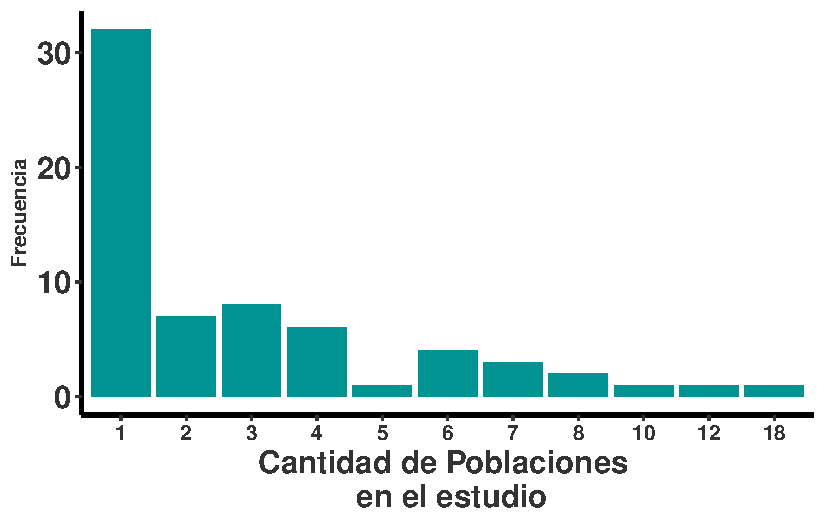
\includegraphics[keepaspectratio]{120-Rage_orquideas_files/figure-pdf/Rage8-1.pdf}}

\begin{center}\rule{0.5\linewidth}{0.5pt}\end{center}

\subsection{La cantidad de poblaciones por especies en la base de datos
de
COMPADRE.}\label{la-cantidad-de-poblaciones-por-especies-en-la-base-de-datos-de-compadre.}

La cantidad de poblaciones muestreadas por especie en la base de datos
de COMPADRE varía considerablemente. Aunque la mayoría de las especies
están representadas por una sola población, existen casos en los que se
han registrado hasta 20 poblaciones distintas para una misma especie.
Estas poblaciones pueden provenir de diferentes publicaciones
científicas o representar datos recolectados en distintos momentos o con
distintos objetivos dentro de una misma población. Por ejemplo, los
datos de \emph{Lepanthes rupestris} provienen de dos estudios
independientes (Tremblay \& Ackerman, 2001; Tremblay \& McCarthy, 2014).
En el primero, se utilizaron matrices poblacionales para estimar el
tamaño efectivo de las poblaciones (Ne), mientras que en el segundo se
emplearon los mismos datos para desarrollar un enfoque bayesiano que
permite estimar los elementos de las matrices de transición,
especialmente útil cuando se dispone de pocos datos por población o
periodo. Este enfoque aprovecha la información conjunta de todas las
poblaciones para generar estimaciones más robustas y biológicamente
realistas.

\begin{center}\rule{0.5\linewidth}{0.5pt}\end{center}

\subsection{¿Cuán largos fueron los
estudios?}\label{cuuxe1n-largos-fueron-los-estudios}

La duración de los estudios en la base de datos de orquídeas de COMPADRE
varía considerablemente. Aunque muchos estudios abarcan solo unos pocos
años ---el mínimo requerido para calcular una matriz de transición
poblacional es de dos periodos---, también existen investigaciones que
se extienden por lapsos más prolongados. Algunos estudios, como los
realizados por Tremblay con \emph{Lepanthes rupestris}, incluyen
muestreos mensuales, mientras que otros se basan en observaciones
anuales. Esta diversidad en la temporalidad refleja tanto los objetivos
específicos de cada investigación como las estrategias metodológicas
empleadas.

La siguiente visualización muestra cómo varía la duración de los
estudios según el tipo de orquídea, diferenciando entre especies
epífitas y terrestres:

\begin{Shaded}
\begin{Highlighting}[]
\NormalTok{SPECIES\_O}\SpecialCharTok{$}\NormalTok{SpeciesAccepted }\OtherTok{\textless{}{-}} \FunctionTok{fct\_reorder}\NormalTok{(}
\NormalTok{  SPECIES\_O}\SpecialCharTok{$}\NormalTok{SpeciesAccepted,}
\NormalTok{  SPECIES\_O}\SpecialCharTok{$}\NormalTok{StudyStart,}
  \AttributeTok{.desc =} \ConstantTok{FALSE}
\NormalTok{)}

\FunctionTok{ggplot}\NormalTok{(SPECIES\_O, }\FunctionTok{aes}\NormalTok{(SpeciesAccepted, }\AttributeTok{ymin =}\NormalTok{ StudyStart, }\AttributeTok{ymax =}\NormalTok{ StudyEnd, }\AttributeTok{color =}\NormalTok{ OrganismType\_RC)) }\SpecialCharTok{+}
  \FunctionTok{geom\_linerange}\NormalTok{() }\SpecialCharTok{+}
  \FunctionTok{coord\_flip}\NormalTok{() }\SpecialCharTok{+}
  \FunctionTok{theme}\NormalTok{(}\AttributeTok{legend.position.inside =} \FunctionTok{c}\NormalTok{(}\FloatTok{0.2}\NormalTok{, }\FloatTok{0.8}\NormalTok{)) }\SpecialCharTok{+}
  \FunctionTok{ylab}\NormalTok{(}\StringTok{""}\NormalTok{) }\SpecialCharTok{+}
  \FunctionTok{xlab}\NormalTok{(}\StringTok{""}\NormalTok{) }\SpecialCharTok{+}
  \FunctionTok{rlt\_style\_colour}\NormalTok{() }\SpecialCharTok{+}
  \FunctionTok{theme}\NormalTok{(}
    \AttributeTok{axis.text.x =} \FunctionTok{element\_text}\NormalTok{(}
      \AttributeTok{color =} \StringTok{"grey20"}\NormalTok{,}
      \AttributeTok{size =} \DecValTok{9}\NormalTok{,}
      \AttributeTok{angle =} \DecValTok{90}\NormalTok{,}
      \AttributeTok{hjust =}\NormalTok{ .}\DecValTok{5}\NormalTok{,}
      \AttributeTok{vjust =}\NormalTok{ .}\DecValTok{5}\NormalTok{,}
      \AttributeTok{face =} \StringTok{"plain"}
\NormalTok{    ),}
    \AttributeTok{axis.text.y =} \FunctionTok{element\_text}\NormalTok{(}
      \AttributeTok{color =} \StringTok{"grey20"}\NormalTok{,}
      \AttributeTok{size =} \DecValTok{7}\NormalTok{,}
      \AttributeTok{angle =} \DecValTok{0}\NormalTok{,}
      \AttributeTok{hjust =} \DecValTok{1}\NormalTok{,}
      \AttributeTok{vjust =} \DecValTok{0}\NormalTok{,}
      \AttributeTok{face =} \StringTok{"plain"}
\NormalTok{    ),}
    \AttributeTok{axis.title.x =} \FunctionTok{element\_text}\NormalTok{(}
      \AttributeTok{color =} \StringTok{"grey20"}\NormalTok{,}
      \AttributeTok{size =} \DecValTok{12}\NormalTok{,}
      \AttributeTok{angle =} \DecValTok{0}\NormalTok{,}
      \AttributeTok{hjust =}\NormalTok{ .}\DecValTok{5}\NormalTok{,}
      \AttributeTok{vjust =} \DecValTok{0}\NormalTok{,}
      \AttributeTok{face =} \StringTok{"plain"}
\NormalTok{    ),}
    \AttributeTok{axis.title.y =} \FunctionTok{element\_text}\NormalTok{(}
      \AttributeTok{color =} \StringTok{"grey20"}\NormalTok{,}
      \AttributeTok{size =} \DecValTok{12}\NormalTok{,}
      \AttributeTok{angle =} \DecValTok{90}\NormalTok{,}
      \AttributeTok{hjust =}\NormalTok{ .}\DecValTok{5}\NormalTok{,}
      \AttributeTok{vjust =}\NormalTok{ .}\DecValTok{5}\NormalTok{,}
      \AttributeTok{face =} \StringTok{"plain"}
\NormalTok{    )}
\NormalTok{  )}\SpecialCharTok{+}
  \FunctionTok{theme}\NormalTok{(}\AttributeTok{legend.position =} \FunctionTok{c}\NormalTok{(}\FloatTok{0.2}\NormalTok{,}\FloatTok{0.8}\NormalTok{),}
        \AttributeTok{legend.title =} \FunctionTok{element\_blank}\NormalTok{())}\SpecialCharTok{+}
  \FunctionTok{theme}\NormalTok{(}\AttributeTok{axis.text.y =} \FunctionTok{element\_text}\NormalTok{(}\AttributeTok{size =} \DecValTok{5}\NormalTok{))}\SpecialCharTok{+}
  \FunctionTok{scale\_y\_continuous}\NormalTok{(}\AttributeTok{n.breaks =} \DecValTok{12}\NormalTok{)}
\end{Highlighting}
\end{Shaded}

\pandocbounded{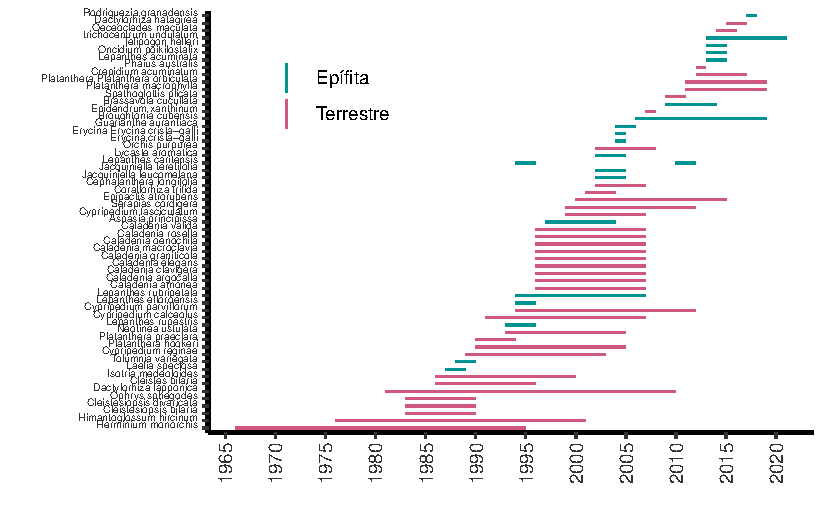
\includegraphics[keepaspectratio]{120-Rage_orquideas_files/figure-pdf/Rage9-1.pdf}}

\begin{Shaded}
\begin{Highlighting}[]
\CommentTok{\#ggsave("images/Lenght\_survey.png")}
\end{Highlighting}
\end{Shaded}

\begin{center}\rule{0.5\linewidth}{0.5pt}\end{center}

\subsection{Tiempo de duración de las
investigaciones.}\label{tiempo-de-duraciuxf3n-de-las-investigaciones.}

La siguiente figura muestra la duración de los estudios realizados sobre
orquídeas epífitas y terrestres. Según los datos extraídos de la base de
datos COMPADRE, la mayoría de las investigaciones tuvieron una duración
relativamente corta, especialmente en el caso de las especies epífitas.
Sin embargo, también se registran estudios que se extendieron por más de
20 años, lo que evidencia un compromiso a largo plazo en algunos casos
para entender mejor la dinámica poblacional de estas plantas.

\begin{Shaded}
\begin{Highlighting}[]
\NormalTok{Orquideas }\OtherTok{=}\NormalTok{ Orquideas }\SpecialCharTok{\%\textgreater{}\%}
  \FunctionTok{mutate}\NormalTok{(}\AttributeTok{StudyDuration =} \FunctionTok{as.numeric}\NormalTok{(StudyDuration),}
    \AttributeTok{OrganismType\_RC =} \FunctionTok{fct\_recode}\NormalTok{(}
\NormalTok{      OrganismType,}
      \StringTok{"Epífita"} \OtherTok{=} \StringTok{"Epiphyte"}\NormalTok{,}
      \StringTok{"Terrestre"} \OtherTok{=} \StringTok{"Herbaceous perennial"}
\NormalTok{    )}
\NormalTok{  )}

\CommentTok{\#table(Orquideas$StudyDuration)}
\CommentTok{\#table(Orquideas$OrganismType)}

\FunctionTok{ggplot}\NormalTok{(Orquideas, }\FunctionTok{aes}\NormalTok{(StudyDuration, }\AttributeTok{fill =}\NormalTok{ OrganismType\_RC)) }\SpecialCharTok{+}
  \FunctionTok{geom\_histogram}\NormalTok{(}\AttributeTok{colour =} \StringTok{"white"}\NormalTok{) }\SpecialCharTok{+}
  \FunctionTok{facet\_wrap}\NormalTok{(}\SpecialCharTok{\textasciitilde{}}\NormalTok{OrganismType\_RC) }\SpecialCharTok{+}
  \FunctionTok{theme}\NormalTok{(}\AttributeTok{legend.position =} \StringTok{"none"}\NormalTok{) }\SpecialCharTok{+}
  \FunctionTok{xlab}\NormalTok{(}\StringTok{"Duración de los estudios"}\NormalTok{) }\SpecialCharTok{+}
  \FunctionTok{ylab}\NormalTok{(}\StringTok{"Frecuencia"}\NormalTok{) }\SpecialCharTok{+}
  \FunctionTok{rlt\_style\_fill}\NormalTok{() }\SpecialCharTok{+}
  \FunctionTok{scale\_x\_continuous}\NormalTok{(}\AttributeTok{n.breaks =} \DecValTok{10}\NormalTok{)}
\end{Highlighting}
\end{Shaded}

\pandocbounded{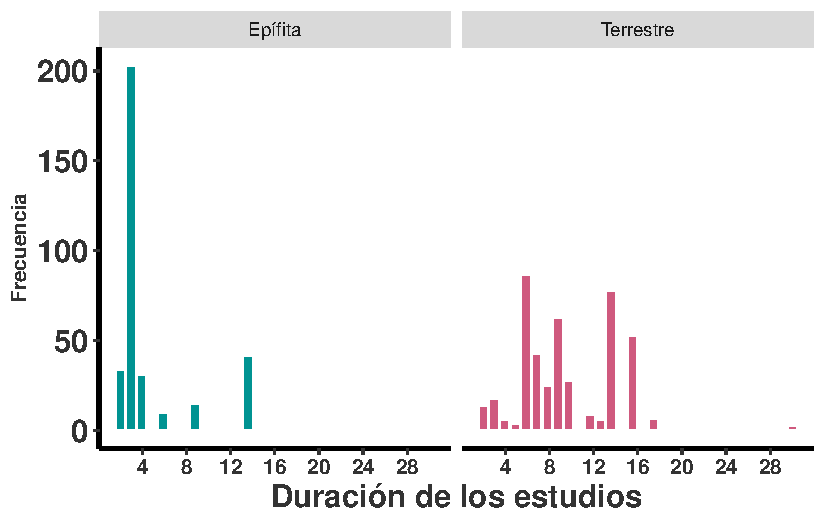
\includegraphics[keepaspectratio]{120-Rage_orquideas_files/figure-pdf/Rage10-1.pdf}}

\begin{Shaded}
\begin{Highlighting}[]
\CommentTok{\#ggsave("Duración\_Epi\_Ter.pdf")}

\FunctionTok{ggsave}\NormalTok{(}\StringTok{"images/Duración\_Epi\_Ter.png"}\NormalTok{)}
\end{Highlighting}
\end{Shaded}

\begin{center}\rule{0.5\linewidth}{0.5pt}\end{center}

\begin{center}\rule{0.5\linewidth}{0.5pt}\end{center}

\subsection{Cálculo del Valor Propio Dominante (λ) en Matrices Ergódicas
e
Irreducibles}\label{cuxe1lculo-del-valor-propio-dominante-ux3bb-en-matrices-erguxf3dicas-e-irreducibles}

A partir del conjunto de matrices previamente filtradas por cumplir con
las condiciones de ergodicidad e irreducibilidad, se procede al cálculo
del valor propio dominante (\(\lambda\)), el cual representa la tasa de
crecimiento poblacional asintótica en modelos matriciales.

Para ello, se emplea la función eigs del paquete popdemo, que permite
obtener los valores propios de una matriz. Esta función se aplica a cada
matriz seleccionada mediante sapply, generando una lista de valores de
(\(\lambda\)) almacenados en el objeto lambdaVals. Cada entrada en esta
lista corresponde al valor propio dominante de una matriz matA incluida
en el conjunto de datos.

Posteriormente, se utiliza la función summary para obtener una
descripción estadística de los valores de (\(\lambda\)), y la función
hist para visualizar su distribución, lo que permite evaluar la
variabilidad en las tasas de crecimiento poblacional entre las distintas
especies o poblaciones representadas.

\subsubsection{Matrices ergódicas e
irreductibles}\label{matrices-erguxf3dicas-e-irreductibles-1}

\begin{landscape}

\begin{Shaded}
\begin{Highlighting}[]
\NormalTok{Compadre\_flagged }\OtherTok{\textless{}{-}} \FunctionTok{cdb\_flag}\NormalTok{(Orquideas)}

\NormalTok{Mat\_erg\_irred }\OtherTok{\textless{}{-}} \FunctionTok{subset}\NormalTok{(}
\NormalTok{  Compadre\_flagged,}
\NormalTok{  check\_NA\_A }\SpecialCharTok{==} \ConstantTok{FALSE} \SpecialCharTok{\&}\NormalTok{ check\_irreducible }\SpecialCharTok{==} \ConstantTok{TRUE} \SpecialCharTok{\&}\NormalTok{ check\_ergodic }\SpecialCharTok{==} \ConstantTok{TRUE}
\NormalTok{) }\CommentTok{\# para evaluar si las matrices son ergódicas e irreducibles al mismo tiempo}

\FunctionTok{head}\NormalTok{(}\FunctionTok{cdb\_metadata}\NormalTok{(Mat\_erg\_irred), }\AttributeTok{n=}\DecValTok{2}\NormalTok{) }\SpecialCharTok{|\textgreater{}}
  \FunctionTok{flextable}\NormalTok{() }\SpecialCharTok{|\textgreater{}} \FunctionTok{ft\_wide}\NormalTok{()}
\end{Highlighting}
\end{Shaded}

\global\setlength{\Oldarrayrulewidth}{\arrayrulewidth}

\global\setlength{\Oldtabcolsep}{\tabcolsep}

\setlength{\tabcolsep}{2pt}

\renewcommand*{\arraystretch}{1.5}



\providecommand{\ascline}[3]{\noalign{\global\arrayrulewidth #1}\arrayrulecolor[HTML]{#2}\cline{#3}}

\begin{longtable*}[c]{cccccccccc}



\ascline{1.5pt}{666666}{1-10}

\multicolumn{1}{>{}r}{\textcolor[HTML]{000000}{\fontsize{6}{6}\selectfont{MatrixID}}} & \multicolumn{1}{>{}l}{\textcolor[HTML]{000000}{\fontsize{6}{6}\selectfont{SpeciesAuthor}}} & \multicolumn{1}{>{}l}{\textcolor[HTML]{000000}{\fontsize{6}{6}\selectfont{SpeciesAccepted}}} & \multicolumn{1}{>{}l}{\textcolor[HTML]{000000}{\fontsize{6}{6}\selectfont{CommonName}}} & \multicolumn{1}{>{}l}{\textcolor[HTML]{000000}{\fontsize{6}{6}\selectfont{Kingdom}}} & \multicolumn{1}{>{}l}{\textcolor[HTML]{000000}{\fontsize{6}{6}\selectfont{Phylum}}} & \multicolumn{1}{>{}l}{\textcolor[HTML]{000000}{\fontsize{6}{6}\selectfont{Class}}} & \multicolumn{1}{>{}l}{\textcolor[HTML]{000000}{\fontsize{6}{6}\selectfont{Order}}} & \multicolumn{1}{>{}l}{\textcolor[HTML]{000000}{\fontsize{6}{6}\selectfont{Family}}} & \multicolumn{1}{>{}l}{\textcolor[HTML]{000000}{\fontsize{6}{6}\selectfont{Genus}}} \\

\ascline{1.5pt}{666666}{1-10}\endfirsthead 

\ascline{1.5pt}{666666}{1-10}

\multicolumn{1}{>{}r}{\textcolor[HTML]{000000}{\fontsize{6}{6}\selectfont{MatrixID}}} & \multicolumn{1}{>{}l}{\textcolor[HTML]{000000}{\fontsize{6}{6}\selectfont{SpeciesAuthor}}} & \multicolumn{1}{>{}l}{\textcolor[HTML]{000000}{\fontsize{6}{6}\selectfont{SpeciesAccepted}}} & \multicolumn{1}{>{}l}{\textcolor[HTML]{000000}{\fontsize{6}{6}\selectfont{CommonName}}} & \multicolumn{1}{>{}l}{\textcolor[HTML]{000000}{\fontsize{6}{6}\selectfont{Kingdom}}} & \multicolumn{1}{>{}l}{\textcolor[HTML]{000000}{\fontsize{6}{6}\selectfont{Phylum}}} & \multicolumn{1}{>{}l}{\textcolor[HTML]{000000}{\fontsize{6}{6}\selectfont{Class}}} & \multicolumn{1}{>{}l}{\textcolor[HTML]{000000}{\fontsize{6}{6}\selectfont{Order}}} & \multicolumn{1}{>{}l}{\textcolor[HTML]{000000}{\fontsize{6}{6}\selectfont{Family}}} & \multicolumn{1}{>{}l}{\textcolor[HTML]{000000}{\fontsize{6}{6}\selectfont{Genus}}} \\

\ascline{1.5pt}{666666}{1-10}\endhead



\multicolumn{10}{>{}l}{\textcolor[HTML]{000000}{\fontsize{7}{7}\selectfont{\textit{Nota:\ se\ muestran\ 10\ de\ 73\ columnas\ disponibles.}}}} \\

\endlastfoot



\multicolumn{1}{>{}r}{\textcolor[HTML]{000000}{\fontsize{6}{6}\selectfont{238,285}}} & \multicolumn{1}{>{}l}{\textcolor[HTML]{000000}{\fontsize{6}{6}\selectfont{Caladenia\_amonea}}} & \multicolumn{1}{>{}l}{\textcolor[HTML]{000000}{\fontsize{6}{6}\selectfont{Caladenia\ amonea}}} & \multicolumn{1}{>{}l}{\textcolor[HTML]{000000}{\fontsize{6}{6}\selectfont{}}} & \multicolumn{1}{>{}l}{\textcolor[HTML]{000000}{\fontsize{6}{6}\selectfont{Plantae}}} & \multicolumn{1}{>{}l}{\textcolor[HTML]{000000}{\fontsize{6}{6}\selectfont{Tracheophyta}}} & \multicolumn{1}{>{}l}{\textcolor[HTML]{000000}{\fontsize{6}{6}\selectfont{Liliopsida}}} & \multicolumn{1}{>{}l}{\textcolor[HTML]{000000}{\fontsize{6}{6}\selectfont{Asparagales}}} & \multicolumn{1}{>{}l}{\textcolor[HTML]{000000}{\fontsize{6}{6}\selectfont{Orchidaceae}}} & \multicolumn{1}{>{}l}{\textcolor[HTML]{000000}{\fontsize{6}{6}\selectfont{Caladenia}}} \\





\multicolumn{1}{>{}r}{\textcolor[HTML]{000000}{\fontsize{6}{6}\selectfont{238,286}}} & \multicolumn{1}{>{}l}{\textcolor[HTML]{000000}{\fontsize{6}{6}\selectfont{Caladenia\_argocalla}}} & \multicolumn{1}{>{}l}{\textcolor[HTML]{000000}{\fontsize{6}{6}\selectfont{Caladenia\ argocalla}}} & \multicolumn{1}{>{}l}{\textcolor[HTML]{000000}{\fontsize{6}{6}\selectfont{}}} & \multicolumn{1}{>{}l}{\textcolor[HTML]{000000}{\fontsize{6}{6}\selectfont{Plantae}}} & \multicolumn{1}{>{}l}{\textcolor[HTML]{000000}{\fontsize{6}{6}\selectfont{Tracheophyta}}} & \multicolumn{1}{>{}l}{\textcolor[HTML]{000000}{\fontsize{6}{6}\selectfont{Liliopsida}}} & \multicolumn{1}{>{}l}{\textcolor[HTML]{000000}{\fontsize{6}{6}\selectfont{Asparagales}}} & \multicolumn{1}{>{}l}{\textcolor[HTML]{000000}{\fontsize{6}{6}\selectfont{Orchidaceae}}} & \multicolumn{1}{>{}l}{\textcolor[HTML]{000000}{\fontsize{6}{6}\selectfont{Caladenia}}} \\

\ascline{1.5pt}{666666}{1-10}



\end{longtable*}



\arrayrulecolor[HTML]{000000}

\global\setlength{\arrayrulewidth}{\Oldarrayrulewidth}

\global\setlength{\tabcolsep}{\Oldtabcolsep}

\renewcommand*{\arraystretch}{1}

\end{landscape}

\begin{Shaded}
\begin{Highlighting}[]
\NormalTok{lambdaVals\_list }\OtherTok{\textless{}{-}} \FunctionTok{sapply}\NormalTok{(}\FunctionTok{matA}\NormalTok{(Mat\_erg\_irred), popdemo}\SpecialCharTok{::}\NormalTok{eigs, }\AttributeTok{what =} \StringTok{"lambda"}\NormalTok{) }

\NormalTok{lambdaVals}\OtherTok{=}\FunctionTok{as\_tibble}\NormalTok{(lambdaVals\_list)}

\FunctionTok{tidy}\NormalTok{(lambdaVals) }\SpecialCharTok{|\textgreater{}} \FunctionTok{flextable}\NormalTok{()}
\end{Highlighting}
\end{Shaded}

\global\setlength{\Oldarrayrulewidth}{\arrayrulewidth}

\global\setlength{\Oldtabcolsep}{\tabcolsep}

\setlength{\tabcolsep}{2pt}

\renewcommand*{\arraystretch}{1.5}



\providecommand{\ascline}[3]{\noalign{\global\arrayrulewidth #1}\arrayrulecolor[HTML]{#2}\cline{#3}}

\begin{longtable*}[c]{ccccccccccccc}



\ascline{1.5pt}{666666}{1-13}

\multicolumn{1}{>{}l}{\textcolor[HTML]{000000}{\fontsize{11}{11}\selectfont{column}}} & \multicolumn{1}{>{}r}{\textcolor[HTML]{000000}{\fontsize{11}{11}\selectfont{n}}} & \multicolumn{1}{>{}r}{\textcolor[HTML]{000000}{\fontsize{11}{11}\selectfont{mean}}} & \multicolumn{1}{>{}r}{\textcolor[HTML]{000000}{\fontsize{11}{11}\selectfont{sd}}} & \multicolumn{1}{>{}r}{\textcolor[HTML]{000000}{\fontsize{11}{11}\selectfont{median}}} & \multicolumn{1}{>{}r}{\textcolor[HTML]{000000}{\fontsize{11}{11}\selectfont{trimmed}}} & \multicolumn{1}{>{}r}{\textcolor[HTML]{000000}{\fontsize{11}{11}\selectfont{mad}}} & \multicolumn{1}{>{}r}{\textcolor[HTML]{000000}{\fontsize{11}{11}\selectfont{min}}} & \multicolumn{1}{>{}r}{\textcolor[HTML]{000000}{\fontsize{11}{11}\selectfont{max}}} & \multicolumn{1}{>{}r}{\textcolor[HTML]{000000}{\fontsize{11}{11}\selectfont{range}}} & \multicolumn{1}{>{}r}{\textcolor[HTML]{000000}{\fontsize{11}{11}\selectfont{skew}}} & \multicolumn{1}{>{}r}{\textcolor[HTML]{000000}{\fontsize{11}{11}\selectfont{kurtosis}}} & \multicolumn{1}{>{}r}{\textcolor[HTML]{000000}{\fontsize{11}{11}\selectfont{se}}} \\

\ascline{1.5pt}{666666}{1-13}\endfirsthead 

\ascline{1.5pt}{666666}{1-13}

\multicolumn{1}{>{}l}{\textcolor[HTML]{000000}{\fontsize{11}{11}\selectfont{column}}} & \multicolumn{1}{>{}r}{\textcolor[HTML]{000000}{\fontsize{11}{11}\selectfont{n}}} & \multicolumn{1}{>{}r}{\textcolor[HTML]{000000}{\fontsize{11}{11}\selectfont{mean}}} & \multicolumn{1}{>{}r}{\textcolor[HTML]{000000}{\fontsize{11}{11}\selectfont{sd}}} & \multicolumn{1}{>{}r}{\textcolor[HTML]{000000}{\fontsize{11}{11}\selectfont{median}}} & \multicolumn{1}{>{}r}{\textcolor[HTML]{000000}{\fontsize{11}{11}\selectfont{trimmed}}} & \multicolumn{1}{>{}r}{\textcolor[HTML]{000000}{\fontsize{11}{11}\selectfont{mad}}} & \multicolumn{1}{>{}r}{\textcolor[HTML]{000000}{\fontsize{11}{11}\selectfont{min}}} & \multicolumn{1}{>{}r}{\textcolor[HTML]{000000}{\fontsize{11}{11}\selectfont{max}}} & \multicolumn{1}{>{}r}{\textcolor[HTML]{000000}{\fontsize{11}{11}\selectfont{range}}} & \multicolumn{1}{>{}r}{\textcolor[HTML]{000000}{\fontsize{11}{11}\selectfont{skew}}} & \multicolumn{1}{>{}r}{\textcolor[HTML]{000000}{\fontsize{11}{11}\selectfont{kurtosis}}} & \multicolumn{1}{>{}r}{\textcolor[HTML]{000000}{\fontsize{11}{11}\selectfont{se}}} \\

\ascline{1.5pt}{666666}{1-13}\endhead



\multicolumn{1}{>{}l}{\textcolor[HTML]{000000}{\fontsize{11}{11}\selectfont{value}}} & \multicolumn{1}{>{}r}{\textcolor[HTML]{000000}{\fontsize{11}{11}\selectfont{491}}} & \multicolumn{1}{>{}r}{\textcolor[HTML]{000000}{\fontsize{11}{11}\selectfont{0.9835195}}} & \multicolumn{1}{>{}r}{\textcolor[HTML]{000000}{\fontsize{11}{11}\selectfont{0.1378241}}} & \multicolumn{1}{>{}r}{\textcolor[HTML]{000000}{\fontsize{11}{11}\selectfont{0.9939963}}} & \multicolumn{1}{>{}r}{\textcolor[HTML]{000000}{\fontsize{11}{11}\selectfont{0.9862572}}} & \multicolumn{1}{>{}r}{\textcolor[HTML]{000000}{\fontsize{11}{11}\selectfont{0.04496007}}} & \multicolumn{1}{>{}r}{\textcolor[HTML]{000000}{\fontsize{11}{11}\selectfont{0.3887968}}} & \multicolumn{1}{>{}r}{\textcolor[HTML]{000000}{\fontsize{11}{11}\selectfont{1.776031}}} & \multicolumn{1}{>{}r}{\textcolor[HTML]{000000}{\fontsize{11}{11}\selectfont{1.387234}}} & \multicolumn{1}{>{}r}{\textcolor[HTML]{000000}{\fontsize{11}{11}\selectfont{-0.2986587}}} & \multicolumn{1}{>{}r}{\textcolor[HTML]{000000}{\fontsize{11}{11}\selectfont{9.917098}}} & \multicolumn{1}{>{}r}{\textcolor[HTML]{000000}{\fontsize{11}{11}\selectfont{0.006219916}}} \\

\ascline{1.5pt}{666666}{1-13}



\end{longtable*}



\arrayrulecolor[HTML]{000000}

\global\setlength{\arrayrulewidth}{\Oldarrayrulewidth}

\global\setlength{\tabcolsep}{\Oldtabcolsep}

\renewcommand*{\arraystretch}{1}

\begin{Shaded}
\begin{Highlighting}[]
\FunctionTok{ggplot}\NormalTok{(lambdaVals, }\FunctionTok{aes}\NormalTok{(value))}\SpecialCharTok{+}
  \FunctionTok{geom\_histogram}\NormalTok{(}\FunctionTok{aes}\NormalTok{(}\AttributeTok{fill=}\StringTok{"lightblue"}\NormalTok{), }\AttributeTok{colour=}\StringTok{"white"}\NormalTok{)}\SpecialCharTok{+}
  \FunctionTok{rlt\_style\_fill}\NormalTok{()}\SpecialCharTok{+}
  \FunctionTok{xlab}\NormalTok{(}\StringTok{"Lambda"}\NormalTok{)}\SpecialCharTok{+}
  \FunctionTok{ylab}\NormalTok{(}\StringTok{"Frecuencia"}\NormalTok{)}\SpecialCharTok{+}
  \FunctionTok{scale\_x\_continuous}\NormalTok{(}\AttributeTok{n.breaks =} \DecValTok{10}\NormalTok{)}\SpecialCharTok{+}
  \FunctionTok{theme}\NormalTok{(}\AttributeTok{legend.position =} \StringTok{"none"}\NormalTok{)}
\end{Highlighting}
\end{Shaded}

\pandocbounded{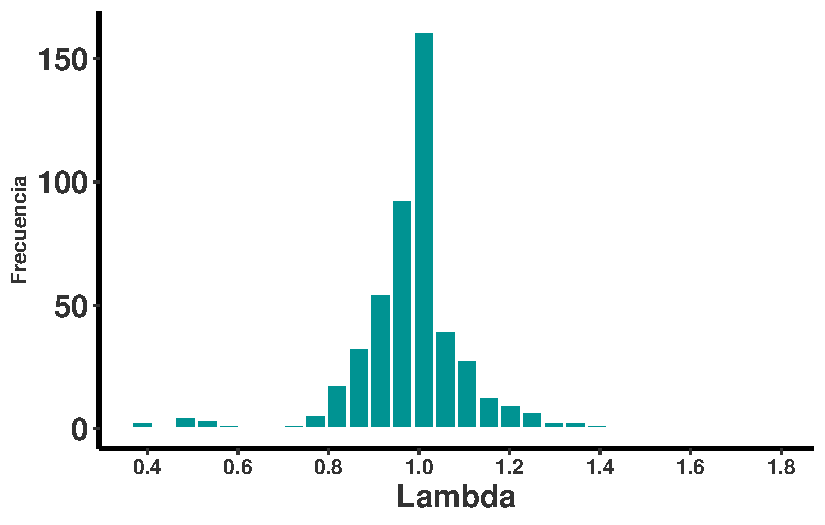
\includegraphics[keepaspectratio]{120-Rage_orquideas_files/figure-pdf/Rage13-1.pdf}}

Una metodología alternativa para calcular los valores propios dominantes
(\(\lambda\)) de las matrices de transición poblacional consiste en
utilizar la función \texttt{map\_dbl} de la librería purrr. Esta función
permite aplicar una operación a cada elemento de una lista, devolviendo
un vector numérico de igual longitud. En este contexto, se aplica una
función de cálculo de \(\lambda\) a cada matriz de transición (matA),
obteniendo así un valor de \(\lambda\) por matriz. Esta estrategia
resulta eficiente para el procesamiento simultáneo de múltiples matrices
dentro de un flujo de trabajo reproducible en R.

\begin{Shaded}
\begin{Highlighting}[]
\DocumentationTok{\#\# con el paquete popdemo}
\NormalTok{lambdaVals1 }\OtherTok{\textless{}{-}} \FunctionTok{map\_dbl}\NormalTok{(}
  \FunctionTok{matA}\NormalTok{(Mat\_erg\_irred),}
  \SpecialCharTok{\textasciitilde{}}\NormalTok{ popdemo}\SpecialCharTok{::}\FunctionTok{eigs}\NormalTok{(.x, }\AttributeTok{what =} \StringTok{"lambda"}\NormalTok{)}
\NormalTok{)}

\DocumentationTok{\#\# O puede calcular lambda con el paquete popbio, que evita algunos mensajes de advertencia}

\NormalTok{lambdaVals2 }\OtherTok{\textless{}{-}} \FunctionTok{map\_dbl}\NormalTok{(}\FunctionTok{matA}\NormalTok{(Mat\_erg\_irred), }\SpecialCharTok{\textasciitilde{}}\NormalTok{ popbio}\SpecialCharTok{::}\FunctionTok{lambda}\NormalTok{(.x))}
\end{Highlighting}
\end{Shaded}

\begin{center}\rule{0.5\linewidth}{0.5pt}\end{center}

\section{\texorpdfstring{Demografía con
\texttt{Rage}}{Demografía con Rage}}\label{demografuxeda-con-rage}

Hasta este punto hemos usado \texttt{Rcompadre} para acceder y filtrar
matrices, y \texttt{popbio}/\texttt{popdemo} para calcular \(\lambda\).
El paquete \texttt{Rage} complementa este flujo con funciones que
derivan estadísticos demográficos directamente de las matrices U, F y C.
A continuación mostramos tres ejemplos sobre el subconjunto filtrado en
\texttt{Mat\_erg\_irred}.

\begin{tcolorbox}[enhanced jigsaw, arc=.35mm, bottomrule=.15mm, bottomtitle=1mm, breakable, colback=white, colbacktitle=quarto-callout-tip-color!10!white, colframe=quarto-callout-tip-color-frame, coltitle=black, left=2mm, leftrule=.75mm, opacityback=0, opacitybacktitle=0.6, rightrule=.15mm, title=\textcolor{quarto-callout-tip-color}{\faLightbulb}\hspace{0.5em}{Recordatorio sobre las submatrices}, titlerule=0mm, toprule=.15mm, toptitle=1mm]

Las funciones de \texttt{Rage} requieren que las matrices estén
descompuestas en sus partes (U = supervivencia/crecimiento, F =
fecundidad sexual, C = crecimiento clonal). Por eso se extraen con
\texttt{matU()}, \texttt{matF()} y \texttt{matC()} en lugar de usar la
matriz completa A.

\end{tcolorbox}

\subsection{Esperanza de vida --- ¿cuánto vive un
individuo?}\label{esperanza-de-vida-cuuxe1nto-vive-un-individuo}

\textbf{Pregunta biológica.} Dado que un individuo sobrevive su etapa
inicial (plántula), ¿cuánto tiempo vive en promedio?
\texttt{life\_expect\_mean()} lo calcula a partir de la matriz U,
modelándola como una cadena de Markov absorbente donde ``muerte'' es el
estado absorbente.

\begin{Shaded}
\begin{Highlighting}[]
\NormalTok{esperanza\_vida }\OtherTok{\textless{}{-}} \FunctionTok{map\_dbl}\NormalTok{(}
  \FunctionTok{matU}\NormalTok{(Mat\_erg\_irred),}
  \SpecialCharTok{\textasciitilde{}} \FunctionTok{tryCatch}\NormalTok{(Rage}\SpecialCharTok{::}\FunctionTok{life\_expect\_mean}\NormalTok{(.x, }\AttributeTok{start =} \DecValTok{1}\NormalTok{L),}
             \AttributeTok{error =} \ControlFlowTok{function}\NormalTok{(e) }\ConstantTok{NA\_real\_}\NormalTok{)}
\NormalTok{)}

\FunctionTok{summary}\NormalTok{(esperanza\_vida)}
\end{Highlighting}
\end{Shaded}

\begin{verbatim}
      Min.    1st Qu.     Median       Mean    3rd Qu.       Max.       NA's 
-15787.092      1.841      6.714    -11.664     17.912    635.403         34 
\end{verbatim}

\begin{tcolorbox}[enhanced jigsaw, arc=.35mm, bottomrule=.15mm, bottomtitle=1mm, breakable, colback=white, colbacktitle=quarto-callout-tip-color!10!white, colframe=quarto-callout-tip-color-frame, coltitle=black, left=2mm, leftrule=.75mm, opacityback=0, opacitybacktitle=0.6, rightrule=.15mm, title=\textcolor{quarto-callout-tip-color}{\faLightbulb}\hspace{0.5em}{Interpretación}, titlerule=0mm, toprule=.15mm, toptitle=1mm]

Una esperanza de vida alta (\textgreater{} 30 pasos de tiempo) indica
una especie longeva con mortalidad adulta baja ---típico de orquídeas
epífitas adultas establecidas. Valores bajos (\textless{} 5 pasos de
tiempo) sugieren mortalidad juvenil dominante, lo que es esperable
cuando \texttt{start\ =\ 1L} corresponde a plántulas con supervivencia
baja. Si el valor parece irrealista, verifique: (1) que \texttt{start}
apunte a la etapa correcta, y (2) que la matriz U no contenga valores de
supervivencia perfecta (ver el capítulo sobre datos sin sentido
biológico).

\end{tcolorbox}

\subsection{Tiempo generacional --- ¿cada cuánto se reemplaza la
población?}\label{tiempo-generacional-cada-cuuxe1nto-se-reemplaza-la-poblaciuxf3n}

\textbf{Pregunta biológica.} ¿Cuántos años (o pasos de tiempo) pasan
entre que un individuo nace y produce su descendencia ``promedio''? Es
la unidad fundamental para comparar la velocidad evolutiva entre
especies. \texttt{gen\_time()} combina la matriz U
(supervivencia/crecimiento) con la matriz F (reproducción).

\begin{Shaded}
\begin{Highlighting}[]
\NormalTok{tiempo\_gen }\OtherTok{\textless{}{-}} \FunctionTok{map2\_dbl}\NormalTok{(}
  \FunctionTok{matU}\NormalTok{(Mat\_erg\_irred),}
  \FunctionTok{matF}\NormalTok{(Mat\_erg\_irred),}
  \SpecialCharTok{\textasciitilde{}} \FunctionTok{tryCatch}\NormalTok{(Rage}\SpecialCharTok{::}\FunctionTok{gen\_time}\NormalTok{(.x, .y),}
             \AttributeTok{error =} \ControlFlowTok{function}\NormalTok{(e) }\ConstantTok{NA\_real\_}\NormalTok{)}
\NormalTok{)}

\FunctionTok{summary}\NormalTok{(tiempo\_gen)}
\end{Highlighting}
\end{Shaded}

\begin{verbatim}
   Min. 1st Qu.  Median    Mean 3rd Qu.    Max.    NA's 
   -Inf   13.82   36.34     NaN  124.90     Inf      41 
\end{verbatim}

\begin{tcolorbox}[enhanced jigsaw, arc=.35mm, bottomrule=.15mm, bottomtitle=1mm, breakable, colback=white, colbacktitle=quarto-callout-tip-color!10!white, colframe=quarto-callout-tip-color-frame, coltitle=black, left=2mm, leftrule=.75mm, opacityback=0, opacitybacktitle=0.6, rightrule=.15mm, title=\textcolor{quarto-callout-tip-color}{\faLightbulb}\hspace{0.5em}{Interpretación}, titlerule=0mm, toprule=.15mm, toptitle=1mm]

Un tiempo generacional alto (\textgreater{} 10) indica especies
``lentas'', longevas, con generaciones traslapadas ---el patrón típico
de orquídeas epífitas perennes. Tiempos bajos (\textless{} 2) sugieren
especies ``rápidas'' con ciclos cortos ---raras en orquídeas, comunes en
hierbas anuales. Las orquídeas terrestres templadas y las epífitas
tropicales suelen ubicarse en el rango 5--25, dependiendo de la
longevidad observada. Comparar tiempos generacionales entre poblaciones
de la misma especie en hábitats distintos es una forma poderosa de
detectar diferenciación demográfica local.

\end{tcolorbox}

\subsection{Edad de primera reproducción --- ¿cuándo arranca la
reproducción?}\label{edad-de-primera-reproducciuxf3n-cuuxe1ndo-arranca-la-reproducciuxf3n}

\textbf{Pregunta biológica.} ¿A qué edad llega un individuo, en
promedio, a su primera etapa reproductiva? Es un componente clave de las
estrategias de historia de vida ---la diferencia entre ``rápido y
arriesgado'' y ``lento y seguro''. \texttt{mature\_age()} integra a
través de la matriz U partiendo de la etapa \texttt{start}.

\begin{Shaded}
\begin{Highlighting}[]
\NormalTok{edad\_madurez }\OtherTok{\textless{}{-}} \FunctionTok{map2\_dbl}\NormalTok{(}
  \FunctionTok{matU}\NormalTok{(Mat\_erg\_irred),}
  \FunctionTok{matF}\NormalTok{(Mat\_erg\_irred),}
  \SpecialCharTok{\textasciitilde{}} \FunctionTok{tryCatch}\NormalTok{(Rage}\SpecialCharTok{::}\FunctionTok{mature\_age}\NormalTok{(.x, .y, }\AttributeTok{start =} \DecValTok{1}\NormalTok{L),}
             \AttributeTok{error =} \ControlFlowTok{function}\NormalTok{(e) }\ConstantTok{NA\_real\_}\NormalTok{)}
\NormalTok{)}

\FunctionTok{summary}\NormalTok{(edad\_madurez)}
\end{Highlighting}
\end{Shaded}

\begin{verbatim}
   Min. 1st Qu.  Median    Mean 3rd Qu.    Max.    NA's 
  1.000   4.908   7.306  11.322  10.075 111.000      85 
\end{verbatim}

\begin{tcolorbox}[enhanced jigsaw, arc=.35mm, bottomrule=.15mm, bottomtitle=1mm, breakable, colback=white, colbacktitle=quarto-callout-tip-color!10!white, colframe=quarto-callout-tip-color-frame, coltitle=black, left=2mm, leftrule=.75mm, opacityback=0, opacitybacktitle=0.6, rightrule=.15mm, title=\textcolor{quarto-callout-tip-color}{\faLightbulb}\hspace{0.5em}{Interpretación}, titlerule=0mm, toprule=.15mm, toptitle=1mm]

En orquídeas terrestres templadas se han documentado edades de primera
reproducción de 5--15 años; en epífitas tropicales el rango puede ser
similar o mayor. Comparar \texttt{mature\_age} con
\texttt{life\_expect\_mean} da el ``esfuerzo prereproductivo'' relativo:
si un individuo gasta el 40\% de su vida esperada antes de reproducirse,
la mortalidad juvenil tiene un peso desproporcionado en la dinámica
poblacional ---y por tanto en cualquier estrategia de conservación.

\end{tcolorbox}

\begin{tcolorbox}[enhanced jigsaw, arc=.35mm, bottomrule=.15mm, bottomtitle=1mm, breakable, colback=white, colbacktitle=quarto-callout-warning-color!10!white, colframe=quarto-callout-warning-color-frame, coltitle=black, left=2mm, leftrule=.75mm, opacityback=0, opacitybacktitle=0.6, rightrule=.15mm, title=\textcolor{quarto-callout-warning-color}{\faExclamationTriangle}\hspace{0.5em}{Cómo defender estos números frente a una revisión crítica}, titlerule=0mm, toprule=.15mm, toptitle=1mm]

Las tres métricas anteriores son robustas matemáticamente pero
\textbf{sensibles} a tres decisiones del modelador: 1. \textbf{Etapa
inicial (\texttt{start}).} ¿Está reportando esperanza de vida desde la
semilla, la plántula, o el adulto recién reclutado? Especifique siempre.
2. \textbf{Calidad de la matriz U.} Si \texttt{colSums(matU)\ ==\ 1}
para alguna columna (supervivencia perfecta ---ver capítulo sobre datos
sin sentido biológico), las tres métricas se inflan artificialmente. La
esperanza de vida puede tender a infinito. 3. \textbf{Reproducción
clonal vs.~sexual.} Si la mayoría de la reproducción ocurre en
\texttt{matC} (clonal) y \texttt{matF} está casi vacía,
\texttt{gen\_time()} y \texttt{mature\_age()} no representan lo que el
lector espera. Reporte ambas matrices y, si la clonalidad domina,
considere usar \texttt{matU\ +\ matC} en lugar de
\texttt{matU\ +\ matF}.

\end{tcolorbox}

\begin{center}\rule{0.5\linewidth}{0.5pt}\end{center}

\section{Variación en el crecimiento poblacional entre especies epífitas
y
terrestres}\label{variaciuxf3n-en-el-crecimiento-poblacional-entre-especies-epuxedfitas-y-terrestres}

En esta sección se seleccionan las especies clasificadas como epífitas y
terrestres, agrupándolas en objetos distintos que contienen todas las
poblaciones muestreadas correspondientes. Esta separación permite
evaluar comparativamente la variación en las tasas de crecimiento
poblacional entre ambos grupos funcionales, facilitando el análisis de
patrones ecológicos y demográficos asociados a sus respectivos hábitos
de vida.

\begin{tcolorbox}[enhanced jigsaw, arc=.35mm, bottomrule=.15mm, bottomtitle=1mm, breakable, colback=white, colbacktitle=quarto-callout-warning-color!10!white, colframe=quarto-callout-warning-color-frame, coltitle=black, left=2mm, leftrule=.75mm, opacityback=0, opacitybacktitle=0.6, rightrule=.15mm, title=\textcolor{quarto-callout-warning-color}{\faExclamationTriangle}\hspace{0.5em}{Cuidado con la pseudoreplicación}, titlerule=0mm, toprule=.15mm, toptitle=1mm]

Cada matriz de COMPADRE corresponde a una combinación específica de
población, año y especie. Una sola especie puede aportar muchas
matrices, de modo que comparar directamente los \(\lambda\) entre grupos
(epífitas vs.~terrestres) sin tener en cuenta esta estructura jerárquica
subestima la varianza real y puede inflar las diferencias aparentes.
Para inferencias formales conviene usar modelos mixtos con la especie
(y, idealmente, la población) como efecto aleatorio.

\end{tcolorbox}

\begin{Shaded}
\begin{Highlighting}[]
\NormalTok{epifitas }\OtherTok{=}\NormalTok{ Orquideas }\SpecialCharTok{\%\textgreater{}\%}
  \FunctionTok{filter}\NormalTok{(OrganismType }\SpecialCharTok{==} \StringTok{"Epiphyte"}\NormalTok{)}

\NormalTok{terrestres }\OtherTok{=}\NormalTok{ Orquideas }\SpecialCharTok{\%\textgreater{}\%}
  \FunctionTok{filter}\NormalTok{(OrganismType }\SpecialCharTok{==} \StringTok{"Herbaceous perennial"}\NormalTok{)}
\end{Highlighting}
\end{Shaded}

\begin{Shaded}
\begin{Highlighting}[]
\NormalTok{Compadre\_flagged\_epif }\OtherTok{\textless{}{-}} \FunctionTok{cdb\_flag}\NormalTok{(epifitas)}

\NormalTok{x\_epif }\OtherTok{\textless{}{-}} \FunctionTok{subset}\NormalTok{(}
\NormalTok{  Compadre\_flagged\_epif,}
\NormalTok{  check\_NA\_A }\SpecialCharTok{==} \ConstantTok{FALSE} \SpecialCharTok{\&}\NormalTok{ check\_ergodic }\SpecialCharTok{==} \ConstantTok{TRUE}
\NormalTok{)}

\CommentTok{\#sapply(matA(x\_epi), popdemo::eigs, what="lambda")}

\NormalTok{lambda\_epif }\OtherTok{\textless{}{-}} \FunctionTok{map\_dbl}\NormalTok{(}\FunctionTok{matA}\NormalTok{(x\_epif), }\SpecialCharTok{\textasciitilde{}}\NormalTok{ popdemo}\SpecialCharTok{::}\FunctionTok{eigs}\NormalTok{(.x, }\AttributeTok{what =} \StringTok{"lambda"}\NormalTok{))}

\CommentTok{\#Or with popbio, which avoids some warning messages…}

\NormalTok{Compadre\_flagged\_terrestres }\OtherTok{\textless{}{-}} \FunctionTok{cdb\_flag}\NormalTok{(terrestres)}

\NormalTok{x\_terr }\OtherTok{\textless{}{-}} \FunctionTok{subset}\NormalTok{(}
\NormalTok{  Compadre\_flagged\_terrestres,}
\NormalTok{  check\_NA\_A }\SpecialCharTok{==} \ConstantTok{FALSE} \SpecialCharTok{\&}\NormalTok{ check\_ergodic }\SpecialCharTok{==} \ConstantTok{TRUE}
\NormalTok{)}

\NormalTok{lambda\_terr }\OtherTok{\textless{}{-}} \FunctionTok{map\_dbl}\NormalTok{(}\FunctionTok{matA}\NormalTok{(x\_terr), }\SpecialCharTok{\textasciitilde{}}\NormalTok{ popdemo}\SpecialCharTok{::}\FunctionTok{eigs}\NormalTok{(.x, }\AttributeTok{what =} \StringTok{"lambda"}\NormalTok{))}
\end{Highlighting}
\end{Shaded}

\begin{center}\rule{0.5\linewidth}{0.5pt}\end{center}

\subsection{Evaluación de Tendencias Centrales y Dispersión en Especies
Terrestres y
Epífitas}\label{evaluaciuxf3n-de-tendencias-centrales-y-dispersiuxf3n-en-especies-terrestres-y-epuxedfitas}

Mediante el uso de la función summary, se analizaron las medidas de
tendencia central y dispersión de los valores propios de lambda
correspondientes a especies terrestres y epífitas. Los resultados
indican que las especies terrestres presentan una mayor dispersión en
los valores de lambda en comparación con las especies epífitas. Aunque
los promedios difieren ligeramente entre ambos grupos, las medianas
resultaron ser similares, lo que sugiere patrones demográficos
comparables en términos de centralidad, pero con variabilidad distinta
en su comportamiento poblacional.

\begin{Shaded}
\begin{Highlighting}[]
\FunctionTok{library}\NormalTok{(flextable)}

\CommentTok{\# Calcular resúmenes}
\NormalTok{epif\_summary }\OtherTok{\textless{}{-}} \FunctionTok{summary}\NormalTok{(lambda\_epif)}
\NormalTok{terr\_summary }\OtherTok{\textless{}{-}} \FunctionTok{summary}\NormalTok{(lambda\_terr)}

\CommentTok{\# Unire los resúmenes en un solo data frame}
\NormalTok{combined\_df }\OtherTok{\textless{}{-}} \FunctionTok{rbind}\NormalTok{(}
\NormalTok{  Epífita }\OtherTok{=}\NormalTok{ epif\_summary,}
  \AttributeTok{Terrestre =}\NormalTok{ terr\_summary}
\NormalTok{)}

\CommentTok{\# Convertir a data frame y añadir columna de hábitat}
\NormalTok{combined\_df }\OtherTok{\textless{}{-}} \FunctionTok{as.data.frame}\NormalTok{(combined\_df)}
\NormalTok{combined\_df}\SpecialCharTok{$}\NormalTok{Habit }\OtherTok{\textless{}{-}} \FunctionTok{rownames}\NormalTok{(combined\_df)}

\CommentTok{\# Reordenar columnas}
\NormalTok{combined\_df }\OtherTok{\textless{}{-}}\NormalTok{ combined\_df[, }\FunctionTok{c}\NormalTok{(}\StringTok{"Habit"}\NormalTok{, }\FunctionTok{names}\NormalTok{(epif\_summary))]}

\CommentTok{\# Crear la tabla con flextable}
\FunctionTok{flextable}\NormalTok{(combined\_df)}
\end{Highlighting}
\end{Shaded}

\global\setlength{\Oldarrayrulewidth}{\arrayrulewidth}

\global\setlength{\Oldtabcolsep}{\tabcolsep}

\setlength{\tabcolsep}{2pt}

\renewcommand*{\arraystretch}{1.5}



\providecommand{\ascline}[3]{\noalign{\global\arrayrulewidth #1}\arrayrulecolor[HTML]{#2}\cline{#3}}

\begin{longtable*}[c]{ccccccc}



\ascline{1.5pt}{666666}{1-7}

\multicolumn{1}{>{}l}{\textcolor[HTML]{000000}{\fontsize{11}{11}\selectfont{Habit}}} & \multicolumn{1}{>{}r}{\textcolor[HTML]{000000}{\fontsize{11}{11}\selectfont{Min.}}} & \multicolumn{1}{>{}r}{\textcolor[HTML]{000000}{\fontsize{11}{11}\selectfont{1st\ Qu.}}} & \multicolumn{1}{>{}r}{\textcolor[HTML]{000000}{\fontsize{11}{11}\selectfont{Median}}} & \multicolumn{1}{>{}r}{\textcolor[HTML]{000000}{\fontsize{11}{11}\selectfont{Mean}}} & \multicolumn{1}{>{}r}{\textcolor[HTML]{000000}{\fontsize{11}{11}\selectfont{3rd\ Qu.}}} & \multicolumn{1}{>{}r}{\textcolor[HTML]{000000}{\fontsize{11}{11}\selectfont{Max.}}} \\

\ascline{1.5pt}{666666}{1-7}\endfirsthead 

\ascline{1.5pt}{666666}{1-7}

\multicolumn{1}{>{}l}{\textcolor[HTML]{000000}{\fontsize{11}{11}\selectfont{Habit}}} & \multicolumn{1}{>{}r}{\textcolor[HTML]{000000}{\fontsize{11}{11}\selectfont{Min.}}} & \multicolumn{1}{>{}r}{\textcolor[HTML]{000000}{\fontsize{11}{11}\selectfont{1st\ Qu.}}} & \multicolumn{1}{>{}r}{\textcolor[HTML]{000000}{\fontsize{11}{11}\selectfont{Median}}} & \multicolumn{1}{>{}r}{\textcolor[HTML]{000000}{\fontsize{11}{11}\selectfont{Mean}}} & \multicolumn{1}{>{}r}{\textcolor[HTML]{000000}{\fontsize{11}{11}\selectfont{3rd\ Qu.}}} & \multicolumn{1}{>{}r}{\textcolor[HTML]{000000}{\fontsize{11}{11}\selectfont{Max.}}} \\

\ascline{1.5pt}{666666}{1-7}\endhead



\multicolumn{1}{>{}l}{\textcolor[HTML]{000000}{\fontsize{11}{11}\selectfont{Epífita}}} & \multicolumn{1}{>{}r}{\textcolor[HTML]{000000}{\fontsize{11}{11}\selectfont{0.3887968}}} & \multicolumn{1}{>{}r}{\textcolor[HTML]{000000}{\fontsize{11}{11}\selectfont{0.9690608}}} & \multicolumn{1}{>{}r}{\textcolor[HTML]{000000}{\fontsize{11}{11}\selectfont{0.9950628}}} & \multicolumn{1}{>{}r}{\textcolor[HTML]{000000}{\fontsize{11}{11}\selectfont{0.9776130}}} & \multicolumn{1}{>{}r}{\textcolor[HTML]{000000}{\fontsize{11}{11}\selectfont{1.004671}}} & \multicolumn{1}{>{}r}{\textcolor[HTML]{000000}{\fontsize{11}{11}\selectfont{1.359231}}} \\





\multicolumn{1}{>{}l}{\textcolor[HTML]{000000}{\fontsize{11}{11}\selectfont{Terrestre}}} & \multicolumn{1}{>{}r}{\textcolor[HTML]{000000}{\fontsize{11}{11}\selectfont{0.4088863}}} & \multicolumn{1}{>{}r}{\textcolor[HTML]{000000}{\fontsize{11}{11}\selectfont{0.9295530}}} & \multicolumn{1}{>{}r}{\textcolor[HTML]{000000}{\fontsize{11}{11}\selectfont{0.9992454}}} & \multicolumn{1}{>{}r}{\textcolor[HTML]{000000}{\fontsize{11}{11}\selectfont{0.9988654}}} & \multicolumn{1}{>{}r}{\textcolor[HTML]{000000}{\fontsize{11}{11}\selectfont{1.043194}}} & \multicolumn{1}{>{}r}{\textcolor[HTML]{000000}{\fontsize{11}{11}\selectfont{1.776031}}} \\

\ascline{1.5pt}{666666}{1-7}



\end{longtable*}



\arrayrulecolor[HTML]{000000}

\global\setlength{\arrayrulewidth}{\Oldarrayrulewidth}

\global\setlength{\tabcolsep}{\Oldtabcolsep}

\renewcommand*{\arraystretch}{1}

Para visualizar los datos en una figura de \texttt{ggplot2}, hay que
convertir estas filas en un \emph{data frame} y añadir una columna con
el tipo de hábitat, renombrar la columna lambda y unir los dos
\emph{data frames} en uno solo.

\begin{Shaded}
\begin{Highlighting}[]
\NormalTok{df\_Lamb\_epif }\OtherTok{=} \FunctionTok{as.data.frame}\NormalTok{(lambda\_epif)}
\NormalTok{df\_Lamb\_terr }\OtherTok{=} \FunctionTok{as.data.frame}\NormalTok{(lambda\_terr)}
\end{Highlighting}
\end{Shaded}

Crear una columna con el tipo de hábitat y renombrar la columna lambda

\begin{Shaded}
\begin{Highlighting}[]
\NormalTok{df\_Lamb\_epi }\OtherTok{=}\NormalTok{ df\_Lamb\_epif }\SpecialCharTok{\%\textgreater{}\%}
  \FunctionTok{add\_column}\NormalTok{(}\AttributeTok{Habit\_Type =} \StringTok{"Epífitas"}\NormalTok{) }\SpecialCharTok{\%\textgreater{}\%}
  \FunctionTok{rename}\NormalTok{(}\AttributeTok{lambda =}\NormalTok{ lambda\_epif)}

\NormalTok{df\_Lamb\_terr }\OtherTok{=} \FunctionTok{as.data.frame}\NormalTok{(lambda\_terr)}
\NormalTok{df\_Lamb\_terr }\OtherTok{=}\NormalTok{ df\_Lamb\_terr }\SpecialCharTok{\%\textgreater{}\%}
  \FunctionTok{add\_column}\NormalTok{(}\AttributeTok{Habit\_Type =} \StringTok{"Terrestre"}\NormalTok{) }\SpecialCharTok{\%\textgreater{}\%}
  \FunctionTok{rename}\NormalTok{(}\AttributeTok{lambda =}\NormalTok{ lambda\_terr)}
\end{Highlighting}
\end{Shaded}

Unir los dos data.frame en uno solo

\begin{Shaded}
\begin{Highlighting}[]
\NormalTok{ALL\_Lambdas }\OtherTok{=} \FunctionTok{rbind}\NormalTok{(df\_Lamb\_epi, df\_Lamb\_terr) }\CommentTok{\# unir los dos data frame en uno}
\end{Highlighting}
\end{Shaded}

Visualizar el crecimiento poblacional por tipo de hábitat

\begin{Shaded}
\begin{Highlighting}[]
\FunctionTok{ggplot}\NormalTok{(ALL\_Lambdas, }\FunctionTok{aes}\NormalTok{(lambda, }\AttributeTok{fill =}\NormalTok{ Habit\_Type)) }\SpecialCharTok{+}
  \FunctionTok{geom\_histogram}\NormalTok{(}\AttributeTok{colour =} \StringTok{"white"}\NormalTok{) }\SpecialCharTok{+}
  \FunctionTok{facet\_wrap}\NormalTok{(}\SpecialCharTok{\textasciitilde{}}\NormalTok{Habit\_Type) }\SpecialCharTok{+}
  \FunctionTok{rlt\_style\_fill}\NormalTok{()}\SpecialCharTok{+}
  \FunctionTok{scale\_x\_continuous}\NormalTok{(}\AttributeTok{n.breaks =} \DecValTok{8}\NormalTok{)}\SpecialCharTok{+}
  \FunctionTok{theme}\NormalTok{(}\AttributeTok{axis.text.x =} \FunctionTok{element\_text}\NormalTok{(}\AttributeTok{angle =} \DecValTok{45}\NormalTok{, }\AttributeTok{hjust =} \DecValTok{1}\NormalTok{))}\SpecialCharTok{+}
  \FunctionTok{ylab}\NormalTok{(}\StringTok{"Frecuencia"}\NormalTok{)}
\end{Highlighting}
\end{Shaded}

\pandocbounded{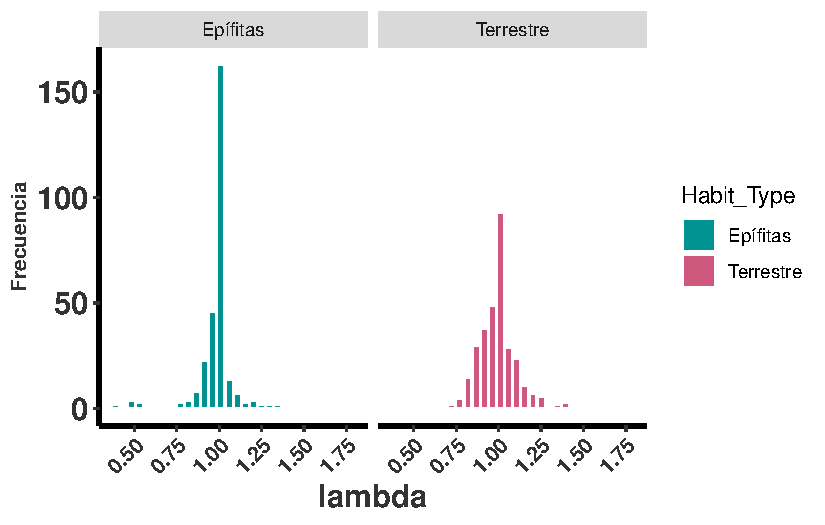
\includegraphics[keepaspectratio]{120-Rage_orquideas_files/figure-pdf/Rage29-1.pdf}}

\begin{Shaded}
\begin{Highlighting}[]
\CommentTok{\# ggsave("images/Terr\_Epi\_lambda.png")}
\end{Highlighting}
\end{Shaded}

\begin{center}\rule{0.5\linewidth}{0.5pt}\end{center}

\section{Estimación del crecimiento promedio y evaluación de diferencias
significativas}\label{estimaciuxf3n-del-crecimiento-promedio-y-evaluaciuxf3n-de-diferencias-significativas}

Para evaluar si existen diferencias significativas en los valores
propios de lambda entre especies epífitas y terrestres, se emplea un
modelo lineal utilizando la función \texttt{lm}. En este análisis, la
variable \textbf{Habit\_Type} se utiliza como predictor del valor propio
dominante (\(\lambda\)), lo que permite estimar el efecto del tipo de
hábitat sobre la tasa de crecimiento poblacional. Los resultados del
modelo indican que las especies epífitas tienden a presentar valores de
lambda más bajos en comparación con las especies terrestres. Para
obtener los coeficientes específicos de cada grupo, se ajusta un segundo
modelo excluyendo el intercepto mediante la inclusión de \texttt{-1} en
la fórmula. Esta parametrización permite calcular directamente el
promedio de lambda para cada grupo funcional, facilitando la comparación
entre ellos.

\begin{tcolorbox}[enhanced jigsaw, arc=.35mm, bottomrule=.15mm, bottomtitle=1mm, breakable, colback=white, colbacktitle=quarto-callout-note-color!10!white, colframe=quarto-callout-note-color-frame, coltitle=black, left=2mm, leftrule=.75mm, opacityback=0, opacitybacktitle=0.6, rightrule=.15mm, title=\textcolor{quarto-callout-note-color}{\faInfo}\hspace{0.5em}{¿Modelar \(\lambda\) o \(\log(\lambda)\)?}, titlerule=0mm, toprule=.15mm, toptitle=1mm]

Los valores de \(\lambda\) son estrictamente positivos y su escala es
multiplicativa: \(\lambda = 1\) separa crecimiento de declive y los
desvíos por arriba (1.2) y por abajo (0.8) no son simétricos. Por eso
muchos demógrafos prefieren modelar \(\log(\lambda)\) (o
\(r = \log(\lambda)\)), que sí es simétrico alrededor de cero, suele
cumplir mejor los supuestos de normalidad, y conecta directamente con la
teoría de crecimiento estocástico (ver el capítulo de simulaciones).
Para el ajuste mostrado aquí podrías usar
\texttt{lm(log(lambda)\ \textasciitilde{}\ Habit\_Type,\ data\ =\ ALL\_Lambdas)}.

\end{tcolorbox}

\begin{Shaded}
\begin{Highlighting}[]
\NormalTok{model\_lambda }\OtherTok{=} \FunctionTok{lm}\NormalTok{(lambda }\SpecialCharTok{\textasciitilde{}}\NormalTok{ Habit\_Type, }\AttributeTok{data =}\NormalTok{ ALL\_Lambdas)}
\CommentTok{\#summary(model\_lambda)}

\NormalTok{model\_lambda\_epi\_terr }\OtherTok{=} \FunctionTok{lm}\NormalTok{(lambda }\SpecialCharTok{\textasciitilde{}}\NormalTok{ Habit\_Type}\DecValTok{{-}1}\NormalTok{, }\AttributeTok{data =}\NormalTok{ ALL\_Lambdas)}
\CommentTok{\#summary(model\_lambda\_epi\_terr)}

\NormalTok{tidy\_results}\OtherTok{=} \FunctionTok{tidy}\NormalTok{(model\_lambda\_epi\_terr)}

\FunctionTok{flextable}\NormalTok{(tidy\_results)}
\end{Highlighting}
\end{Shaded}

\global\setlength{\Oldarrayrulewidth}{\arrayrulewidth}

\global\setlength{\Oldtabcolsep}{\tabcolsep}

\setlength{\tabcolsep}{2pt}

\renewcommand*{\arraystretch}{1.5}



\providecommand{\ascline}[3]{\noalign{\global\arrayrulewidth #1}\arrayrulecolor[HTML]{#2}\cline{#3}}

\begin{longtable*}[c]{ccccc}



\ascline{1.5pt}{666666}{1-5}

\multicolumn{1}{>{}l}{\textcolor[HTML]{000000}{\fontsize{11}{11}\selectfont{term}}} & \multicolumn{1}{>{}r}{\textcolor[HTML]{000000}{\fontsize{11}{11}\selectfont{estimate}}} & \multicolumn{1}{>{}r}{\textcolor[HTML]{000000}{\fontsize{11}{11}\selectfont{std.error}}} & \multicolumn{1}{>{}r}{\textcolor[HTML]{000000}{\fontsize{11}{11}\selectfont{statistic}}} & \multicolumn{1}{>{}r}{\textcolor[HTML]{000000}{\fontsize{11}{11}\selectfont{p.value}}} \\

\ascline{1.5pt}{666666}{1-5}\endfirsthead 

\ascline{1.5pt}{666666}{1-5}

\multicolumn{1}{>{}l}{\textcolor[HTML]{000000}{\fontsize{11}{11}\selectfont{term}}} & \multicolumn{1}{>{}r}{\textcolor[HTML]{000000}{\fontsize{11}{11}\selectfont{estimate}}} & \multicolumn{1}{>{}r}{\textcolor[HTML]{000000}{\fontsize{11}{11}\selectfont{std.error}}} & \multicolumn{1}{>{}r}{\textcolor[HTML]{000000}{\fontsize{11}{11}\selectfont{statistic}}} & \multicolumn{1}{>{}r}{\textcolor[HTML]{000000}{\fontsize{11}{11}\selectfont{p.value}}} \\

\ascline{1.5pt}{666666}{1-5}\endhead



\multicolumn{1}{>{}l}{\textcolor[HTML]{000000}{\fontsize{11}{11}\selectfont{Habit\_TypeEpífitas}}} & \multicolumn{1}{>{}r}{\textcolor[HTML]{000000}{\fontsize{11}{11}\selectfont{0.9776130}}} & \multicolumn{1}{>{}r}{\textcolor[HTML]{000000}{\fontsize{11}{11}\selectfont{0.007781499}}} & \multicolumn{1}{>{}r}{\textcolor[HTML]{000000}{\fontsize{11}{11}\selectfont{125.633}}} & \multicolumn{1}{>{}r}{\textcolor[HTML]{000000}{\fontsize{11}{11}\selectfont{0}}} \\





\multicolumn{1}{>{}l}{\textcolor[HTML]{000000}{\fontsize{11}{11}\selectfont{Habit\_TypeTerrestre}}} & \multicolumn{1}{>{}r}{\textcolor[HTML]{000000}{\fontsize{11}{11}\selectfont{0.9988654}}} & \multicolumn{1}{>{}r}{\textcolor[HTML]{000000}{\fontsize{11}{11}\selectfont{0.007387240}}} & \multicolumn{1}{>{}r}{\textcolor[HTML]{000000}{\fontsize{11}{11}\selectfont{135.215}}} & \multicolumn{1}{>{}r}{\textcolor[HTML]{000000}{\fontsize{11}{11}\selectfont{0}}} \\

\ascline{1.5pt}{666666}{1-5}



\end{longtable*}



\arrayrulecolor[HTML]{000000}

\global\setlength{\arrayrulewidth}{\Oldarrayrulewidth}

\global\setlength{\tabcolsep}{\Oldtabcolsep}

\renewcommand*{\arraystretch}{1}

\begin{center}\rule{0.5\linewidth}{0.5pt}\end{center}

\subsection{Visualización de las distribuciones de los
lambda's}\label{visualizaciuxf3n-de-las-distribuciones-de-los-lambdas}

Para representar gráficamente las distribuciones de los coeficientes
estimados en el modelo lineal, se emplean las librerías \texttt{ggdist}
y \texttt{distributional}, utilizando la función \textbf{stat\_halfeye}.
Esta función permite visualizar la forma y dispersión de las
distribuciones de los parámetros, proporcionando una representación
intuitiva de la incertidumbre asociada a cada estimación. Es importante
destacar que stat\_halfeye requiere especificar explícitamente la
distribución de los datos; en este análisis, se asume que los valores
propios de lambda (\(\lambda\)) siguen una distribución normal. La
información utilizada para esta visualización proviene del modelo
ajustado previamente (model\_lambda), lo que permite comparar
directamente los coeficientes entre grupos funcionales como epífitas y
terrestres.

\begin{Shaded}
\begin{Highlighting}[]
\NormalTok{model\_lambda\_epi\_terr }\SpecialCharTok{\%\textgreater{}\%}
  \FunctionTok{tidy}\NormalTok{() }\SpecialCharTok{\%\textgreater{}\%}
  \FunctionTok{ggplot}\NormalTok{(}\FunctionTok{aes}\NormalTok{(}\AttributeTok{y =}\NormalTok{ term)) }\SpecialCharTok{+}
  \FunctionTok{stat\_halfeye}\NormalTok{(}
    \FunctionTok{aes}\NormalTok{(}
      \AttributeTok{xdist =} \FunctionTok{dist\_student\_t}\NormalTok{(}
        \AttributeTok{df =} \FunctionTok{df.residual}\NormalTok{(model\_lambda\_epi\_terr),}
        \AttributeTok{mu =}\NormalTok{ estimate,}
        \AttributeTok{sigma =}\NormalTok{ std.error}
\NormalTok{      )}
\NormalTok{    )}
\NormalTok{  )}
\end{Highlighting}
\end{Shaded}

\pandocbounded{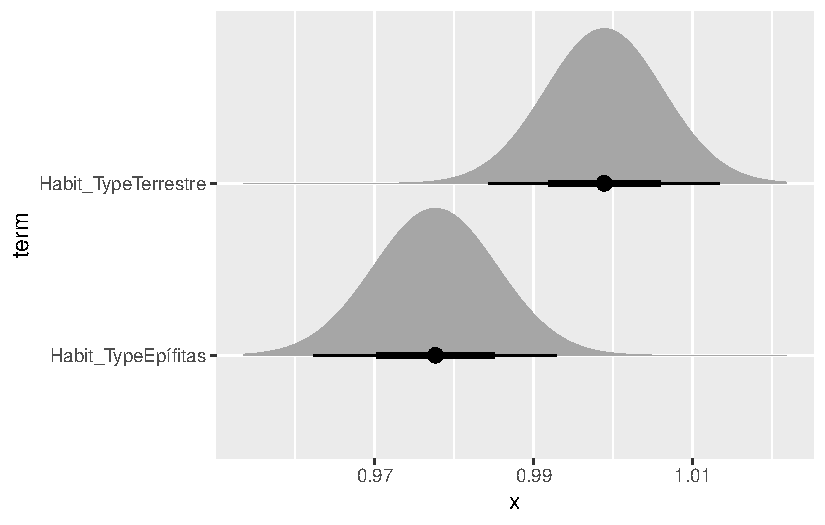
\includegraphics[keepaspectratio]{120-Rage_orquideas_files/figure-pdf/Rage31-1.pdf}}

La gráfica anterior puede ocultar la dispersión de los datos,
especialmente cuando hay sesgos. Para abordar esto, se pueden añadir los
datos originales a la figura. En este caso, se ha incorporado un símbolo
de barra \textbf{\textbar{}} por cada valor de lambda en la parte
inferior de la gráfica. Al observar esta nueva visualización, se nota
que la dispersión varía significativamente si se compara la
representación basada en el promedio y el error estándar con la
distribución real de los datos, representada por los
\textbf{\textbar{}}. Esta figura permite apreciar mejor tanto la
dispersión como la distribución de los datos. En comparación con la
gráfica anterior, esta ofrece una perspectiva más completa, destacando
los valores que se alejan del centro de la distribución.

\begin{Shaded}
\begin{Highlighting}[]
\NormalTok{ALL\_Lambdas }\SpecialCharTok{\%\textgreater{}\%}
  \FunctionTok{expand}\NormalTok{(Habit\_Type) }\SpecialCharTok{\%\textgreater{}\%}
  \FunctionTok{augment}\NormalTok{(model\_lambda, }\AttributeTok{newdata =}\NormalTok{ ., }\AttributeTok{se\_fit =} \ConstantTok{TRUE}\NormalTok{) }\SpecialCharTok{\%\textgreater{}\%}
  \FunctionTok{ggplot}\NormalTok{(}\FunctionTok{aes}\NormalTok{(}\AttributeTok{y =}\NormalTok{ Habit\_Type, }\AttributeTok{colour =}\NormalTok{ Habit\_Type)) }\SpecialCharTok{+}
  \FunctionTok{stat\_halfeye}\NormalTok{(}
    \FunctionTok{aes}\NormalTok{(}
      \AttributeTok{xdist =} \FunctionTok{dist\_student\_t}\NormalTok{(}
        \AttributeTok{df =} \FunctionTok{df.residual}\NormalTok{(model\_lambda),}
        \AttributeTok{mu =}\NormalTok{ .fitted,}
        \AttributeTok{sigma =}\NormalTok{ .se.fit}
\NormalTok{      )}
\NormalTok{    ),}
    \AttributeTok{scale =}\NormalTok{ .}\DecValTok{5}
\NormalTok{  ) }\SpecialCharTok{+}
  \FunctionTok{geom\_point}\NormalTok{(}
    \FunctionTok{aes}\NormalTok{(}\AttributeTok{x =}\NormalTok{ lambda),}
    \AttributeTok{data =}\NormalTok{ ALL\_Lambdas,}
    \AttributeTok{pch =} \StringTok{"|"}\NormalTok{,}
    \AttributeTok{size =} \DecValTok{2}\NormalTok{,}
    \AttributeTok{position =} \FunctionTok{position\_nudge}\NormalTok{(}\AttributeTok{y =} \SpecialCharTok{{-}}\NormalTok{.}\DecValTok{15}\NormalTok{)}
\NormalTok{  )}\SpecialCharTok{+}
  \FunctionTok{theme}\NormalTok{(}\AttributeTok{legend.position =} \FunctionTok{c}\NormalTok{(}\FloatTok{0.1}\NormalTok{, }\FloatTok{0.8}\NormalTok{)) }\SpecialCharTok{+}
  \FunctionTok{rlt\_style\_colour}\NormalTok{()}\SpecialCharTok{+}
  \FunctionTok{ylab}\NormalTok{(}\StringTok{""}\NormalTok{)}
\end{Highlighting}
\end{Shaded}

\pandocbounded{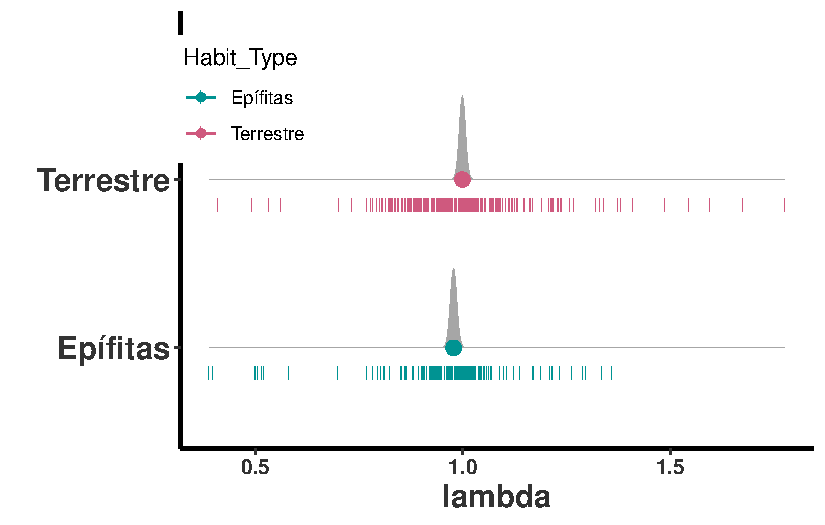
\includegraphics[keepaspectratio]{120-Rage_orquideas_files/figure-pdf/Rage32-1.pdf}}

\begin{center}\rule{0.5\linewidth}{0.5pt}\end{center}

\section{Mapa de distribución de los
estudios.}\label{mapa-de-distribuciuxf3n-de-los-estudios.}

La lista presentada corresponde a los datos extraídos de la base de
datos COMPADRE, complementados con información obtenida directamente de
los artículos científicos, con el objetivo de construir un mapa que
muestre dónde se han realizado estudios de dinámica poblacional.

Lamentablemente, COMPADRE aún carece de muchos datos y detalles
importantes que deberían incorporarse a su base. En esta sección, se
realizó una búsqueda específica de estudios sobre orquídeas dentro de
COMPADRE, extrayendo las coordenadas de latitud y longitud directamente
de los artículos originales.

En los casos en que no se encontraron coordenadas exactas, pero sí se
identificó el país o región del estudio, se utilizó Google Maps para
estimar las coordenadas aproximadas del sitio de muestreo. Cuando no fue
posible obtener ninguna información sobre la localización del estudio,
esos casos fueron excluidos del mapa.

Agradezco a Diana Molina Ozuma por su valiosa colaboración en la
búsqueda de las coordenadas de los sitios de estudio.

\begin{Shaded}
\begin{Highlighting}[]
\NormalTok{Orchid\_data\_DOI\_Diana\_3a }\OtherTok{\textless{}{-}} \FunctionTok{read\_excel}\NormalTok{(}\StringTok{"data/Orchid\_data\_DOI\_Diana\_3a.xlsx"}\NormalTok{)}
\end{Highlighting}
\end{Shaded}

\begin{Shaded}
\begin{Highlighting}[]
\NormalTok{Lat\_Long }\OtherTok{=}\NormalTok{ Orchid\_data\_DOI\_Diana\_3a }\SpecialCharTok{\%\textgreater{}\%}
  \FunctionTok{select}\NormalTok{(SpeciesAccepted, Lon, Lat, OrganismType) }\SpecialCharTok{|\textgreater{}}
  \FunctionTok{distinct}\NormalTok{(SpeciesAccepted, Lon, Lat, OrganismType)}

\CommentTok{\#write\_csv(Lat\_Long, "data/Orchid\_data\_DOI\_Diana\_3a.csv")}
\end{Highlighting}
\end{Shaded}

\begin{center}\rule{0.5\linewidth}{0.5pt}\end{center}

\subsection{Visualización de distribución
geoespacial}\label{visualizaciuxf3n-de-distribuciuxf3n-geoespacial}

Para representar la distribución geográfica de las orquídeas registradas
en la base de datos \texttt{COMPADRE}, se utilizó el paquete
\textbf{ggplot2}. En esta visualización, se emplea la función
\textbf{borders}, que incorpora los contornos de los países al mapa.
Esta función se basa en el paquete maps, el cual proporciona los datos
geográficos necesarios para delinear los límites nacionales, permitiendo
contextualizar espacialmente los puntos de muestreo.

\begin{Shaded}
\begin{Highlighting}[]
\NormalTok{ggplot2}\SpecialCharTok{::}\FunctionTok{ggplot}\NormalTok{(Lat\_Long, }\FunctionTok{aes}\NormalTok{(Lon, Lat, }\AttributeTok{colour =}\NormalTok{ OrganismType)) }\SpecialCharTok{+}
  \FunctionTok{borders}\NormalTok{(}\AttributeTok{database =} \StringTok{"world"}\NormalTok{, }\AttributeTok{fill =} \StringTok{"grey80"}\NormalTok{, }\AttributeTok{colour =} \ConstantTok{NA}\NormalTok{) }\SpecialCharTok{+}
  \FunctionTok{geom\_point}\NormalTok{(}\AttributeTok{size =} \FloatTok{1.0}\NormalTok{, }\AttributeTok{alpha =} \FloatTok{0.5}\NormalTok{)}\SpecialCharTok{+}
  \FunctionTok{theme}\NormalTok{(}\AttributeTok{legend.position =} \FunctionTok{c}\NormalTok{(}\FloatTok{0.15}\NormalTok{,}\FloatTok{0.2}\NormalTok{))}\SpecialCharTok{+}
  \FunctionTok{rlt\_style\_colour}\NormalTok{()}
\end{Highlighting}
\end{Shaded}

\pandocbounded{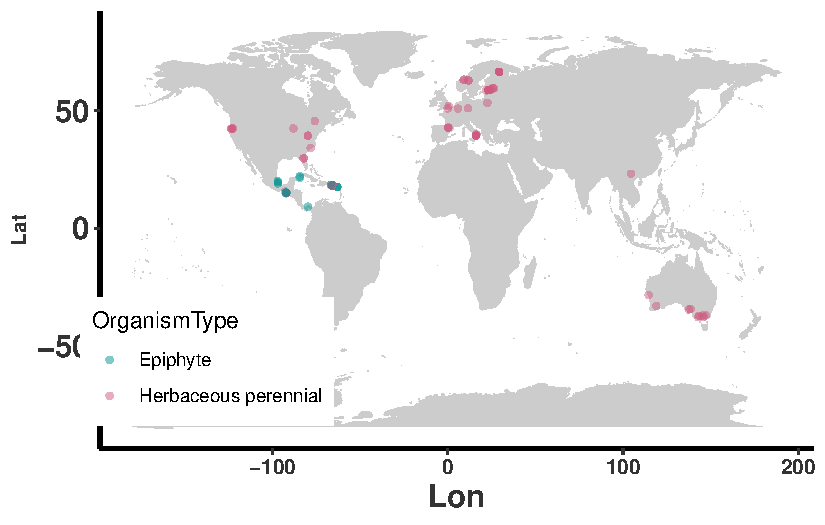
\includegraphics[keepaspectratio]{120-Rage_orquideas_files/figure-pdf/Rage35-1.pdf}}

\begin{Shaded}
\begin{Highlighting}[]
\CommentTok{\#ggsave("orchid\_map.jpg")}
\end{Highlighting}
\end{Shaded}

\begin{center}\rule{0.5\linewidth}{0.5pt}\end{center}

\section{Mapa de distribución interactivo con
Leaflet}\label{mapa-de-distribuciuxf3n-interactivo-con-leaflet}

Se utilizó el paquete Leaflet para crear un mapa interactivo que muestra
los sitios de muestreo de las especies de orquídeas estudiadas en campo.
Este enfoque permite explorar visualmente la distribución geográfica de
las poblaciones incluidas en los estudios.

El mapa revela una marcada disparidad en los sitios de muestreo entre
los dos tipos de orquídeas. Las poblaciones marcadas en rojo
corresponden a especies epífitas, mientras que las azules representan
especies terrestres. Se observa que las especies terrestres están
principalmente distribuidas en Europa y América del Norte, con escasa
representación en Asia y ninguna en África. Por otro lado, las especies
epífitas se concentran en el Caribe y América Central (especialmente
México), sin presencia en África, Asia ni Australia.

\begin{tcolorbox}[enhanced jigsaw, arc=.35mm, bottomrule=.15mm, bottomtitle=1mm, breakable, colback=white, colbacktitle=quarto-callout-important-color!10!white, colframe=quarto-callout-important-color-frame, coltitle=black, left=2mm, leftrule=.75mm, opacityback=0, opacitybacktitle=0.6, rightrule=.15mm, title=\textcolor{quarto-callout-important-color}{\faExclamation}\hspace{0.5em}{Sesgo geográfico de COMPADRE}, titlerule=0mm, toprule=.15mm, toptitle=1mm]

La distribución que se ve en el mapa \textbf{no refleja la diversidad
real de las orquídeas en el mundo}, sino la distribución geográfica del
esfuerzo de investigación demográfica. Regiones con altísima diversidad
de orquídeas (Borneo, Nueva Guinea, los Andes, el África tropical) están
casi ausentes de la base de datos. Cualquier conclusión global sobre
patrones demográficos debe interpretarse con esta limitación en mente:
estamos describiendo \emph{dónde se ha estudiado}, no \emph{dónde
habitan} las orquídeas.

\end{tcolorbox}

Además, el mapa es interactivo y permite hacer zoom para examinar áreas
específicas con mayor detalle. Presiona sobre los puntos para obtener
información adicional sobre el nombre científico de la especie
muestreada en este sitio.

\emph{El mapa interactivo de distribución de orquídeas está disponible
únicamente en la versión HTML del libro.}

\begin{center}\rule{0.5\linewidth}{0.5pt}\end{center}

\section{De la métrica al argumento
biológico}\label{de-la-muxe9trica-al-argumento-bioluxf3gico}

Calcular esperanzas de vida y tiempos generacionales es la mitad fácil.
La mitad difícil ---y la que separa un análisis presentable de uno que
sobrevive la revisión por pares--- es \textbf{construir un argumento
biológico} a partir de las métricas, no sólo reportarlas.

A continuación se ilustra el patrón en cuatro pasos, usando los objetos
calculados arriba (\texttt{esperanza\_vida}, \texttt{tiempo\_gen},
\texttt{edad\_madurez}) sobre el subconjunto filtrado
\texttt{Mat\_erg\_irred}.

\subsection{Paso 1 --- Tabla resumen por hábito de
vida}\label{paso-1-tabla-resumen-por-huxe1bito-de-vida}

Combinamos las tres métricas con el \texttt{OrganismType}
correspondiente para comparar epífitas vs.~terrestres:

\begin{Shaded}
\begin{Highlighting}[]
\CommentTok{\# Construir un data frame con las tres métricas + hábito de vida}
\NormalTok{metricas }\OtherTok{\textless{}{-}} \FunctionTok{tibble}\NormalTok{(}
  \AttributeTok{habito =} \FunctionTok{cdb\_metadata}\NormalTok{(Mat\_erg\_irred)}\SpecialCharTok{$}\NormalTok{OrganismType,}
  \AttributeTok{esperanza\_vida =}\NormalTok{ esperanza\_vida,}
  \AttributeTok{tiempo\_gen =}\NormalTok{ tiempo\_gen,}
  \AttributeTok{edad\_madurez =}\NormalTok{ edad\_madurez}
\NormalTok{) }\SpecialCharTok{\%\textgreater{}\%}
  \FunctionTok{drop\_na}\NormalTok{() }\SpecialCharTok{\%\textgreater{}\%}
  \FunctionTok{mutate}\NormalTok{(}
    \AttributeTok{habito =} \FunctionTok{case\_when}\NormalTok{(}
\NormalTok{      habito }\SpecialCharTok{==} \StringTok{"Epiphyte"} \SpecialCharTok{\textasciitilde{}} \StringTok{"Epífita"}\NormalTok{,}
\NormalTok{      habito }\SpecialCharTok{==} \StringTok{"Herbaceous perennial"} \SpecialCharTok{\textasciitilde{}} \StringTok{"Terrestre"}\NormalTok{,}
      \ConstantTok{TRUE} \SpecialCharTok{\textasciitilde{}}\NormalTok{ habito}
\NormalTok{    )}
\NormalTok{  )}

\CommentTok{\# Resumen por hábito}
\NormalTok{metricas }\SpecialCharTok{\%\textgreater{}\%}
  \FunctionTok{group\_by}\NormalTok{(habito) }\SpecialCharTok{\%\textgreater{}\%}
  \FunctionTok{summarise}\NormalTok{(}
    \AttributeTok{n               =} \FunctionTok{n}\NormalTok{(),}
    \AttributeTok{esperanza\_med   =} \FunctionTok{round}\NormalTok{(}\FunctionTok{median}\NormalTok{(esperanza\_vida, }\AttributeTok{na.rm =} \ConstantTok{TRUE}\NormalTok{), }\DecValTok{2}\NormalTok{),}
    \AttributeTok{tiempo\_gen\_med  =} \FunctionTok{round}\NormalTok{(}\FunctionTok{median}\NormalTok{(tiempo\_gen, }\AttributeTok{na.rm =} \ConstantTok{TRUE}\NormalTok{), }\DecValTok{2}\NormalTok{),}
    \AttributeTok{edad\_madurez\_med =} \FunctionTok{round}\NormalTok{(}\FunctionTok{median}\NormalTok{(edad\_madurez, }\AttributeTok{na.rm =} \ConstantTok{TRUE}\NormalTok{), }\DecValTok{2}\NormalTok{)}
\NormalTok{  ) }\SpecialCharTok{\%\textgreater{}\%}
  \FunctionTok{flextable}\NormalTok{()}
\end{Highlighting}
\end{Shaded}

\global\setlength{\Oldarrayrulewidth}{\arrayrulewidth}

\global\setlength{\Oldtabcolsep}{\tabcolsep}

\setlength{\tabcolsep}{2pt}

\renewcommand*{\arraystretch}{1.5}



\providecommand{\ascline}[3]{\noalign{\global\arrayrulewidth #1}\arrayrulecolor[HTML]{#2}\cline{#3}}

\begin{longtable*}[c]{ccccc}



\ascline{1.5pt}{666666}{1-5}

\multicolumn{1}{>{}l}{\textcolor[HTML]{000000}{\fontsize{11}{11}\selectfont{habito}}} & \multicolumn{1}{>{}r}{\textcolor[HTML]{000000}{\fontsize{11}{11}\selectfont{n}}} & \multicolumn{1}{>{}r}{\textcolor[HTML]{000000}{\fontsize{11}{11}\selectfont{esperanza\_med}}} & \multicolumn{1}{>{}r}{\textcolor[HTML]{000000}{\fontsize{11}{11}\selectfont{tiempo\_gen\_med}}} & \multicolumn{1}{>{}r}{\textcolor[HTML]{000000}{\fontsize{11}{11}\selectfont{edad\_madurez\_med}}} \\

\ascline{1.5pt}{666666}{1-5}\endfirsthead 

\ascline{1.5pt}{666666}{1-5}

\multicolumn{1}{>{}l}{\textcolor[HTML]{000000}{\fontsize{11}{11}\selectfont{habito}}} & \multicolumn{1}{>{}r}{\textcolor[HTML]{000000}{\fontsize{11}{11}\selectfont{n}}} & \multicolumn{1}{>{}r}{\textcolor[HTML]{000000}{\fontsize{11}{11}\selectfont{esperanza\_med}}} & \multicolumn{1}{>{}r}{\textcolor[HTML]{000000}{\fontsize{11}{11}\selectfont{tiempo\_gen\_med}}} & \multicolumn{1}{>{}r}{\textcolor[HTML]{000000}{\fontsize{11}{11}\selectfont{edad\_madurez\_med}}} \\

\ascline{1.5pt}{666666}{1-5}\endhead



\multicolumn{1}{>{}l}{\textcolor[HTML]{000000}{\fontsize{11}{11}\selectfont{Epífita}}} & \multicolumn{1}{>{}r}{\textcolor[HTML]{000000}{\fontsize{11}{11}\selectfont{195}}} & \multicolumn{1}{>{}r}{\textcolor[HTML]{000000}{\fontsize{11}{11}\selectfont{10.28}}} & \multicolumn{1}{>{}r}{\textcolor[HTML]{000000}{\fontsize{11}{11}\selectfont{38.55}}} & \multicolumn{1}{>{}r}{\textcolor[HTML]{000000}{\fontsize{11}{11}\selectfont{7.99}}} \\





\multicolumn{1}{>{}l}{\textcolor[HTML]{000000}{\fontsize{11}{11}\selectfont{Terrestre}}} & \multicolumn{1}{>{}r}{\textcolor[HTML]{000000}{\fontsize{11}{11}\selectfont{185}}} & \multicolumn{1}{>{}r}{\textcolor[HTML]{000000}{\fontsize{11}{11}\selectfont{3.83}}} & \multicolumn{1}{>{}r}{\textcolor[HTML]{000000}{\fontsize{11}{11}\selectfont{26.61}}} & \multicolumn{1}{>{}r}{\textcolor[HTML]{000000}{\fontsize{11}{11}\selectfont{6.84}}} \\

\ascline{1.5pt}{666666}{1-5}



\end{longtable*}



\arrayrulecolor[HTML]{000000}

\global\setlength{\arrayrulewidth}{\Oldarrayrulewidth}

\global\setlength{\tabcolsep}{\Oldtabcolsep}

\renewcommand*{\arraystretch}{1}

\subsection{Paso 2 --- Pregunta
concreta}\label{paso-2-pregunta-concreta}

¿Las epífitas tienen tiempos generacionales más largos que las
terrestres? Si así fuera, sería evidencia de que viven en un régimen
``lento'' (longevidad alta, reproducción tardía) coherente con su hábito
---un sustrato menos predecible favorece el riesgo distribuido a través
de muchos eventos reproductivos pequeños.

\subsection{Paso 3 --- Visualización antes que
estadística}\label{paso-3-visualizaciuxf3n-antes-que-estaduxedstica}

\begin{Shaded}
\begin{Highlighting}[]
\FunctionTok{ggplot}\NormalTok{(metricas, }\FunctionTok{aes}\NormalTok{(}\AttributeTok{x =}\NormalTok{ habito, }\AttributeTok{y =}\NormalTok{ tiempo\_gen, }\AttributeTok{fill =}\NormalTok{ habito)) }\SpecialCharTok{+}
  \FunctionTok{geom\_boxplot}\NormalTok{(}\AttributeTok{alpha =} \FloatTok{0.7}\NormalTok{) }\SpecialCharTok{+}
  \FunctionTok{geom\_jitter}\NormalTok{(}\AttributeTok{width =} \FloatTok{0.15}\NormalTok{, }\AttributeTok{alpha =} \FloatTok{0.5}\NormalTok{) }\SpecialCharTok{+}
  \FunctionTok{ylab}\NormalTok{(}\StringTok{"Tiempo generacional (años)"}\NormalTok{) }\SpecialCharTok{+}
  \FunctionTok{xlab}\NormalTok{(}\StringTok{"Hábito de vida"}\NormalTok{) }\SpecialCharTok{+}
  \FunctionTok{theme}\NormalTok{(}\AttributeTok{legend.position =} \StringTok{"none"}\NormalTok{) }\SpecialCharTok{+}
  \FunctionTok{rlt\_style\_fill}\NormalTok{()}
\end{Highlighting}
\end{Shaded}

\pandocbounded{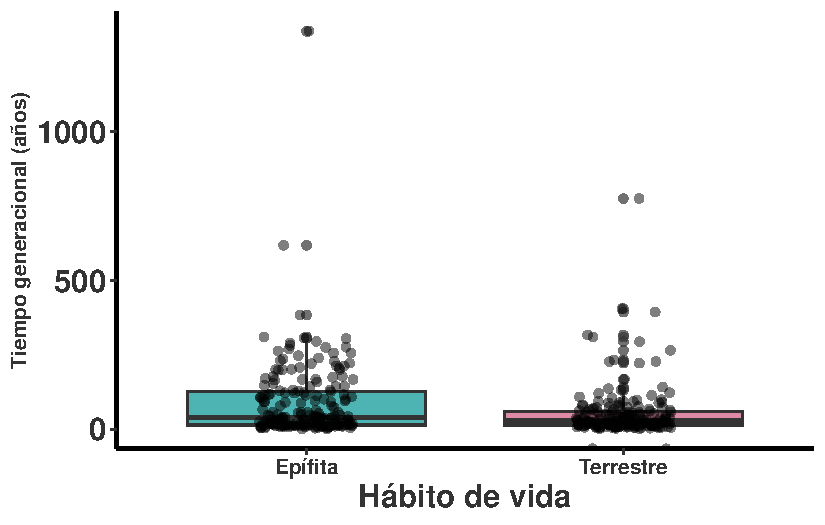
\includegraphics[keepaspectratio]{120-Rage_orquideas_files/figure-pdf/Rage_compare_plot-1.pdf}}

\subsection{Paso 4 --- La discusión que un revisor
pediría}\label{paso-4-la-discusiuxf3n-que-un-revisor-pediruxeda}

Suponga que el gráfico muestra una mediana mayor en epífitas. Antes de
afirmar que esto refleja una diferencia evolutiva real, un revisor
crítico preguntará:

\begin{tcolorbox}[enhanced jigsaw, arc=.35mm, bottomrule=.15mm, bottomtitle=1mm, breakable, colback=white, colbacktitle=quarto-callout-warning-color!10!white, colframe=quarto-callout-warning-color-frame, coltitle=black, left=2mm, leftrule=.75mm, opacityback=0, opacitybacktitle=0.6, rightrule=.15mm, title=\textcolor{quarto-callout-warning-color}{\faExclamationTriangle}\hspace{0.5em}{Las cuatro preguntas que un revisor hará}, titlerule=0mm, toprule=.15mm, toptitle=1mm]

\begin{enumerate}
\def\labelenumi{\arabic{enumi}.}
\tightlist
\item
  \textbf{¿Pseudoreplicación?} Una sola especie (p.~ej. \emph{Lepanthes
  caritensis}) puede contribuir varias matrices del mismo estudio. Si
  esa especie está en uno solo de los grupos, el resultado puede deberse
  a esa especie, no al hábito de vida. Verifíquelo con
  \texttt{count(metricas,\ SpeciesAccepted)} y use modelos mixtos con la
  especie como efecto aleatorio para inferencias formales.
\item
  \textbf{¿Sesgo geográfico?} ¿Las epífitas en su muestra son tropicales
  y las terrestres templadas? La diferencia que ve podría reflejar el
  clima, no el hábito. Mapéelas (sección anterior) y considere agregar
  latitud como covariable.
\item
  \textbf{¿Sesgo de detección?} Las orquídeas terrestres con latencia
  subterránea son menos detectables; sus tiempos generacionales pueden
  estar subestimados si la latencia no se modeló (ver capítulos sobre
  etapas crípticas y fecundidad). Reporte qué especies tienen
  \texttt{MatrixCriteriaOntogeny} con etapas latentes.
\item
  \textbf{¿Calidad de la matriz?} ¿Filtró por \texttt{check\_NA\_A},
  \texttt{check\_ergodic} y \texttt{check\_irreducible}? ¿Las matrices
  que pasaron tienen \texttt{colSums(matU)\ ≤\ 1}? Sin esas garantías,
  los números son numéricamente válidos pero biológicamente sospechosos
  (ver el capítulo sobre datos sin sentido biológico).
\end{enumerate}

\end{tcolorbox}

Un análisis comparativo que \textbf{anticipe} estas cuatro preguntas en
su discusión ---y muestre los gráficos / estadísticas
correspondientes--- es el que sobrevive la revisión por pares. Reportar
la métrica sin enfrentarlas es invitar al rechazo.

\begin{center}\rule{0.5\linewidth}{0.5pt}\end{center}

\section{Ejercicios --- Pruebe usted
mismo}\label{ejercicios-pruebe-usted-mismo-1}

\begin{tcolorbox}[enhanced jigsaw, arc=.35mm, bottomrule=.15mm, bottomtitle=1mm, breakable, colback=white, colbacktitle=quarto-callout-tip-color!10!white, colframe=quarto-callout-tip-color-frame, coltitle=black, left=2mm, leftrule=.75mm, opacityback=0, opacitybacktitle=0.6, rightrule=.15mm, title=\textcolor{quarto-callout-tip-color}{\faLightbulb}\hspace{0.5em}{Ejercicio 1 --- Esperanza de vida por especie}, titlerule=0mm, toprule=.15mm, toptitle=1mm]

Calcule la mediana de la esperanza de vida (\texttt{life\_expect\_mean})
para cada especie de orquídea en COMPADRE con al menos dos matrices.
¿Cuál es la especie con la esperanza de vida más alta? ¿Y la más baja?
¿Tiene sentido biológico?

\end{tcolorbox}

\begin{tcolorbox}[enhanced jigsaw, arc=.35mm, bottomrule=.15mm, bottomtitle=1mm, breakable, colback=white, colbacktitle=quarto-callout-tip-color!10!white, colframe=quarto-callout-tip-color-frame, coltitle=black, left=2mm, leftrule=.75mm, opacityback=0, opacitybacktitle=0.6, rightrule=.15mm, title=\textcolor{quarto-callout-tip-color}{\faLightbulb}\hspace{0.5em}{Ejercicio 2 --- Tiempo generacional \textasciitilde{} longevidad}, titlerule=0mm, toprule=.15mm, toptitle=1mm]

Cree un gráfico de dispersión de \texttt{gen\_time} contra
\texttt{life\_expect\_mean} para todas las matrices del subconjunto.
¿Hay correlación? ¿Qué especies se separan del patrón general?

\end{tcolorbox}

\begin{tcolorbox}[enhanced jigsaw, arc=.35mm, bottomrule=.15mm, bottomtitle=1mm, breakable, colback=white, colbacktitle=quarto-callout-tip-color!10!white, colframe=quarto-callout-tip-color-frame, coltitle=black, left=2mm, leftrule=.75mm, opacityback=0, opacitybacktitle=0.6, rightrule=.15mm, title=\textcolor{quarto-callout-tip-color}{\faLightbulb}\hspace{0.5em}{Ejercicio 3 --- Sensibilidad al \texttt{start}}, titlerule=0mm, toprule=.15mm, toptitle=1mm]

Recalcule \texttt{life\_expect\_mean} con \texttt{start\ =\ 2L}
(juvenil) y \texttt{start\ =\ N} (donde N es la última etapa). Compare
con los resultados originales (\texttt{start\ =\ 1L}). ¿Cuánto cambia?
¿Qué reportaría usted en un manuscrito ---y por qué?

\end{tcolorbox}

\begin{tcolorbox}[enhanced jigsaw, arc=.35mm, bottomrule=.15mm, bottomtitle=1mm, breakable, colback=white, colbacktitle=quarto-callout-tip-color!10!white, colframe=quarto-callout-tip-color-frame, coltitle=black, left=2mm, leftrule=.75mm, opacityback=0, opacitybacktitle=0.6, rightrule=.15mm, title=\textcolor{quarto-callout-tip-color}{\faLightbulb}\hspace{0.5em}{Ejercicio 4 --- Iteroparidad vs.~semelparidad}, titlerule=0mm, toprule=.15mm, toptitle=1mm]

Use \texttt{Rage::entropy\_d()} sobre el subconjunto. ¿Las orquídeas son
más iteróparas (entropía baja) o más semélparas (entropía alta)? Compare
con grupos no-orquídeas usando otro \texttt{Family} en COMPADRE.

\end{tcolorbox}

\bookmarksetup{startatroot}

\chapter{Un protocolo estándar para comunicar información demográfica
estructurada en fases discretas}\label{protocolo}

\subsubsection{Librerías de R requeridas para el siguiente
módulo}\label{libreruxedas-de-r-requeridas-para-el-siguiente-muxf3dulo-15}

\begin{Shaded}
\begin{Highlighting}[]
\FunctionTok{library}\NormalTok{(Rage)}
\FunctionTok{library}\NormalTok{(DiagrammeR)}
\FunctionTok{library}\NormalTok{(tibble)}
\end{Highlighting}
\end{Shaded}

\section{``A standard protocol to report discrete stage-structured
demographic
information''}\label{a-standard-protocol-to-report-discrete-stage-structured-demographic-information}

Samuel J. L. Gascoigne1 \textbar{} Simon Rolph2 \textbar{} Daisy Sankey1
\textbar{} Nagalakshmi Nidadavolu1 \textbar{} Adrian S. Stell Pičman1,3
\textbar{} Christina M. Hernández4 \textbar{} Matthew E. R. Philpott1
\textbar{} Aiyla Salam1 \textbar{} Connor Bernard1 \textbar{} Erola
Fenollosa1 \textbar{} Young Jun Lee1 \textbar{} Jessica McLean1
\textbar{} Shathuki Hetti Achchige Perera1 \textbar{} Oliver G. Spacey1
\textbar{} Maja Kajin1,3 \textbar{} Anna C. Vinton1 \textbar{} C. Ruth
Archer5 \textbar{} Jean H. Burns6 \textbar{} Danielle L. Buss7,8
\textbar{} Hal Caswell9 \textbar{} Judy P. Che-Castaldo10 \textbar{}
Dylan Z. Childs2 \textbar{} Pol Capdevila11 \textbar{} Aldo
Compagnoni1,12,13 \textbar{} Elizabeth Crone14 \textbar{} Thomas H. G.
Ezard15 \textbar{} Dave Hodgson8 \textbar{} Tiffany M. Knight12,13,16
\textbar{} Owen R. Jones17 \textbar{} Eelke Jongejans18,19 \textbar{}
Jenni McDonald20,21 \textbar{} Brigitte Tenhumberg22 \textbar{} Chelsea
C. Thomas23 \textbar{} Andrew J. Tyre2,4,25 \textbar{} Satu Ramula26
\textbar{} Iain Stott27 \textbar{} Raymond L. Tremblay28,29,30
\textbar{} Phil Wilson8 \textbar{} James W. Vaupel31,‡ \textbar{}
Roberto Salguero-Gómez1,32,33

1Department of Biology, University of Oxford, Oxford, UK; 2Department of
Animal \& Plant Sciences, University of Sheffield, Sheffield, UK;
3Department of Biology, University of Ljubljana, Ljubljana, Slovenia;
4Department of Ecology and Evolutionary Biology, Cornell University,
Ithaca, New York, USA; 5Institute of Evolutionary Ecology and
Conservation Genomics, University of Ulm, Ulm, Germany; 6Department of
Biology, Case Western Reserve University, Cleveland, Ohio, USA;
7Department of Archaeology, University of Cambridge, Cambridge, UK;
8College of Life and Environmental Sciences, University of Exeter,
Penryn, UK; 9Institute for Biodiversity and Ecosystem Dynamics,
University of Amsterdam, Amsterdam, The Netherlands; 10Branch of Species
Status Assessment Science Support, U.S. Fish and Wildlife Service,
Washington, DC, USA; 11School of Biological Sciences, University of
Bristol, Bristol, UK; 12Institute of Biology, Martin Luther University
Halle-Wittenburg, Halle (Saale), Germany; 13German Centre for
Integrative Biodiversity Research (iDiv) Halle-Jena-Leipzig, Leipzig,
Germany; 14Department of Biology, Tufts University, Medford,
Massachusetts, USA; 15School of Ocean and Earth Science, University of
Southampton, Southampton, UK; 16Department of Community Ecology,
Helmholtz Centre for Environmental Research-UFZ, Halle (Saale), Germany;
17Department of Biology, University of Southern Denmark, Odense,
Denmark; 18Animal Ecology and Physiology, Radboud University, Nijmegen,
The Netherlands; 19NIOO-KNAW, Animal Ecology, Wageningen, The
Netherlands; 20Veterinary Department, Cats Protection, National Cat
Centre, Haywards Heath, UK; 21Bristol Veterinary School, University of
Bristol, Bristol, UK; 22School of Biological Sciences and Department of
Mathematics, University of Nebraska, Lincoln, Nebraska, USA; 23Alexander
Center for Applied Population Biology, Conservation \& Science
Department, Chicago, Illinois, USA; 24School of Natural Resources,
University of Nebraska-Lincoln, Lincoln, Nebraska, USA; 25Global
Resistance Management Team, Bayer U.S. --Crop Science, Chesterfield,
Missouri, USA; 26Department of Biology, University of Turku, Turku,
Finland; 27School of Life Sciences, University of Lincoln, Lincoln, UK;
28Department of Biology, University of Puerto Rico, San Juan, Puerto
Rico, USA; 29Center for Applied Tropical Ecology and Conservation,
University of Puerto Rico, San Juan, Puerto Rico, USA; 30Department of
Biology, University of Puerto Rico-Humacao, Puerto Rico, USA;
31Interdisciplinary Centre on Population Dynamics, University of
Southern Denmark, Odense, Denmark; 32Centre for Biodiversity and
Conservation Science, University of Queensland, St Lucia, Queensland,
Australia y 33Evolutionary Demography Laboratory, Max Planck Institute
for Demographic Research, Rostock, Germany

Persona de contacto

Samuel J. L. Gascoigne Email: samuel.gascoigne@pmb.ox.ac.uk

Roberto Salguero-Gómez Email: rob.salguero@biology.ox.ac.uk

Traducido por \emph{Raymond L. Tremblay, Roberto Salguero-Gómez, Anne
Damon y Diana Molina Ozuna}

Nota: Cualquier conflicto entre el texto en inglés y español, siempre se
debería dar prioridad al texto en inglés.

Cuando cite el artículo use la siguiente información, ({Gascoigne
et~al.}, 2023)

Abstract

\begin{enumerate}
\def\labelenumi{\arabic{enumi}.}
\item
  Los métodos demográficos que se basan en estadios del ciclo de vida,
  como los Modelos Matriciales Poblacionales (MPP, por sus siglas en
  inglés), son herramientas poderosas que se utilizan para abordar una
  amplia gama de preguntas que son fundamentales en la ecología,
  biología evolutiva y ciencias de la conservación. Debido a su
  potencial, ahora existen MPP para más de 3,000 especies en todo el
  mundo. Estos datos se están digitalizando como un proceso continuo y
  se publican periódicamente en dos grandes repositorios online de forma
  totalmente abierta: la base de datos de matrices de plantas de
  COMPADRE y la base de datos de matrices de animales de COMADRE. Sin
  embargo, durante la última década, el análisis y la curación de los
  datos de COMPADRE y COMADRE, y la investigación comparativa posterior,
  han revelado una variación pronunciada en la forma en que se
  parametrizan y reportan los MPP.
\item
  Aquí resumimos los retos y aspectos de mejora actuales relacionados
  con la parametrización y difusión de los MPP, los que surgen con más
  frecuencia, y describimos cómo afectan la construcción, el análisis y
  la interpretación de los MPP. Para cuantificar la variación en cómo se
  difundan los MPP, presentamos los resultados de una encuesta que
  buscaba identificar aspectos clave de los MPP que con frecuencia no se
  presentan en los manuscritos. Luego evaluamos las bases de datos de
  COMPADRE y COMADRE para cuantificar con qué frecuencia se omiten
  piezas clave de información en los manuscritos donde manejan los MPP.
\item
  Más del 80 \% de los investigadores entrevistados (n = 60) comentaron
  positivamente sobre las ventajas de adoptar metodologías más
  estandarizadas para difundir y compartir los MPP. Además, más del 85\%
  de los 300 MPP evaluados por COMPADRE y COMADRE omitieron uno o más de
  los elementos clave para su correcta interpretación. Basado en estos
  resultados, identificamos los principales problemas que pueden surgir
  a partir de la construcción y difusión de los MPP y ofrecemos
  sugerencias para mejorar la claridad y la reproducibilidad y así
  contribuir a la investigación futura utilizando MPP y los metadatos
  requeridos. Para fortalecer la reproducibilidad y capacitar a los
  investigadores para aprovechar al máximo sus datos demográficos,
  presentamos un protocolo estandarizado para presentar los MPP en las
  publicaciones. Este estándar está vinculado con el contenido de
  www.compadre-db.org, para que los autores que deseen archivar sus MPP
  puedan hacerlo antes de someter sus publicaciones, siguiendo ejemplos
  de otros repositorios de acceso abierto como DRYAD, Figshare y Zenodo.
\item
  La combinación y estandarización de MPP parametrizados provenientes de
  poblaciones de todo el mundo, y de todo el árbol de la vida, abre
  poderosas oportunidades de investigación en la biología evolutiva,
  ecología y conservación. Sin embargo, enfatizamos que este potencial
  solo se logrará mediante la adopción de métodos estandarizados para
  garantizar la reproducibilidad.
\end{enumerate}

PALABRAS CLAVE

demografía comparativa, modelos matriciales de población, acceso
abierto, reproducibilidad.

1 \textbar{} INTRODUCCIÓN

La ecología de poblaciones ha llegado a la mayoría de edad. El
desarrollo de teorías, enfoques experimentales, y metodologías
estadísticas han dado como resultado la publicación de información
demográfica para una muestra cada vez más representativa de la
biodiversidad mundial (De Magalhaes \& Costa, 2009; {Salguero-Gómez
et~al.}, 2015, 2016; Levin et~al., 2022). Estos datos abarcan el árbol
taxonómico desde los microbios (Jouvet, Rodrı́guez-Rojas \& Steiner,
2018) hasta macrovertebrados (Fujiwara \& Caswell, 2001), y cubren
prácticamente todos los continentes y biomas, aunque con importantes
sesgos taxonómicos ({Conde et~al.}, 2019; Römer et~al., 2023). El
potencial de esta cantidad tan impresionante de información y en rápido
aumento está comenzando a realizarse. De hecho, mediante la combinación
de estos modelos demográficos, los investigadores han identificado
características funcionales que explican la variación en las estrategias
de la historia de vida de las plantas (Adler et~al., 2014; ver también
Bernard et~al., 2023), características a corto plazo (transitorias) que
impulsan la evolución demográfica, la dinámica de las poblaciones de
plantas en ambientes variables (McDonald et~al., 2016), y las formas en
que las estrategias de historia de vida permiten que las especies
persistan en un entorno de clima cambiante ({Jelbert et~al.}, 2019;
Paniw et~al., 2019).

Una de las herramientas más utilizadas para describir y analizar las
complejas historias de vida de las especies es la de los modelos de
población matricial (MPP). Brevemente, en un MPP, los individuos de una
población se clasifican por etapas discretas y/o edades (st/edad en
adelante) de acuerdo con algunos criterios biológicos (Caswell, 2001, p.
31) o estadísticos/de muestreo (Salguero-Gómez \& Plotkin, 2010). Estos
individuos son seguidos en pasos de tiempo discretos, típicamente
ajustados por el tiempo generacional de cada especie. De hecho, los
pasos de tiempo pueden variar de 12 a 24 h, como en los gusanos
nematodos \emph{Caenorhabditis elegans} y pulgones \emph{Myzus persicae}
(Li et~al., 2014; Bruijning, Jongejans \& Turcotte, 2019), a períodos
mensuales/anuales en mamíferos y plantas (Coulson et~al., 2001; Ferreira
et~al., 2016), y hasta los 50 años en los ``red woods'' de crecimiento
lento (Namkoong \& Roberds, 1974). A partir de estos datos, los
investigadores estiman probabilidades de supervivencia, probabilidades
de transición entre estadios/edades, y su contribuciones per cápita
a/sexuales a través de la reproducción (Nordstrom, Dykstra \& Wagenius,
2021; Omeyer et~al., 2021).

A partir de un solo MPP se puede calcular un amplio repertorio de
resultados biológicamente interesantes. Estos resultados incluyen
indicadores estimados del desempeño y la viabilidad de las poblaciones,
como tasas de crecimiento demográfico deterministas (γ) o estocásticas
(γs) (Doak et~al., 2005), riesgo de cuasi-extinción (Davis, 2022),
respuesta de la población a perturbaciones de las tasas vitales
subyacentes, como la supervivencia o la reproducción (Fujiwara \&
Caswell, 2001, p. 206), dinámica transitoria Ezard et~al. (2010) y
rasgos de historia de vida, como tasas de senescencia (Baudisch et~al.,
2013), grado de iteroparidad (Salguero-Gomez et~al., 2017) y edad a la
madurez (Fujiwara \& Caswell, 2001, p. 124). Esta gran cantidad de
inferencias demográficas destaca el por qué han sido tan importantes los
MPP para el desarrollo de la demografía y la teoría de la historia de
vida (Tuljapurkar, 1989; Franco \& Silvertown, 1996; Pfister, 1998;
{Sæther et~al.}, 2013).

Los MPP para plantas y animales han sido archivados, corregidos,
complementados con información adicional (p.~ej., coordenadas GPS,
estado de conservación de la UICN) y publicados en medios de acceso
abierto en la Base de Datos de Matrices Vegetales de COMPADRE
({Salguero-Gómez et~al.}, 2015) y la Base de Datos de Matrices Animales
COMADRE ({Salguero-Gómez et~al.}, 2016). En la publicación más reciente,
COMPADRE v. 6.22.5 {[}COMADRE v. 4.21.8{]} se presentan datos de 8851
{[}3317{]} MPP de 760 {[}415{]} especies distintas, trabajadas en 643
{[}395{]} estudios. Al momento de redactar este informe, otras 1307
especies están pendientes de digitalización en la red COMPADRE, con una
tasa aproximada de 4.5 nuevos trabajos que contienen MPP siendo
analizados, digitalizados y pasados por un proceso de control de calidad
cada semana (S. Gascoigne, obs. pers.). Sin embargo, uno de los desafíos
del proceso de digitalización es la enorme variación en la forma en que
se recopilan, presentan y utilizan los datos para parametrizar los MPP.
La estandarización de datos mejora la capacidad de replicación y
facilita el intercambio de datos entre disciplinas de investigación
(Powers \& Hampton, 2019). Por lo tanto, la estandarización de los
datos, y los metadatos detallados asociados, es clave para que la
investigación se replique, valide, y discuta abiertamente para que la
ciencia avance (Reichman, Jones \& Schildhauer, 2011; Powers \& Hampton,
2019; Salguero-Gómez, Jackson \& Gascoigne, 2021). Ejemplos de estos
estándares incluyen, informar del tamaño de la muestra y de la varianza
de las estimaciones, además de detallar la lista completa de fuentes
originales de datos (Gerstner et~al., 2017). En este contexto, los
estándares se pueden utilizar como elementos de una lista de requisitos
para mejorar la calidad y la reproducibilidad de las publicaciones y el
proceso de arbitraje por pares (Reichman, Jones \& Schildhauer, 2011).
Este proceso de estandarización hará posible ampliar el alcance del
análisis, mediante la inclusión de los meta-análisis (Gurevitch et~al.,
2018) y los análisis comparativos filogenéticos (Salguero-Gomez et~al.,
2017; Healy et~al., 2019), que ofrecen oportunidades valiosas para
examinar patrones generales e identificar lagunas en el conocimiento, y
en ambos casos también dependen de datos que conforman a determinadas
normas.

Los MPP se están adaptando, ampliando y aplicando más allá de su
contexto original especie-específica en la demografía comparativa. Sin
embargo, no todos los MPP se construyen y se reporten de la misma
manera. La presentación actual de las MPP en COMPADRE y COMADRE nos
podría dar la falsa impresión de que todos los MPP se conformen a un
formato homogéneo predeterminado, y esto a pesar de las diferencias en
cómo y por qué fueron concebidos los MPP (Caswell, 2001). Esta impresión
pudo haber surgido por el extenso proceso de verificación que realiza el
equipo de digitalización de COMADRE y COMPADRE atrás de las escenas
(p.~ej., validación de los resultados del modelo, correspondencia con el
autor para obtener información adicional). Si bien la verificación es un
aspecto inevitable de la curación de bases de datos, la mayor parte de
nuestros esfuerzos se dedica a comunicarnos con los autores en lugar de
la digitalización de datos. Nuestro objetivo aquí es (i) presentar el
estándar actual de comunicación de los MPP en la literatura, (ii)
identificar problemas comunes en la comunicación de los MPP y sus
impactos, (iii) sugerir formas de apoyar la comunicación clara de datos
y metadatos de los MPP, (iv) destacar las ventajas para los autores y la
comunidad científica en general y (v) introducir un método estándar para
compartir datos y metadatos de los MPP.

2 \textbar{} COMUNICACIÓN MPP: ESTADO DEL ARTE

Para presentar las prácticas actuales en la comunicación de datos y
metadatos de los MPP, con el objetivo final de evaluar la necesidad de
estandarizar informes de datos y metadatos, realizamos una encuesta de
investigadores y examinamos un subconjunto de publicaciones que se han
utilizado para generar MPMs y que han sido almacenados en COMPADRE y
COMADRE.

2.1 \textbar{} Una encuesta sobre comunicación matricial

Entrevistamos especialistas de ecología de poblaciones, a quienes
identificamos por haber publicado artículos revisados por pares que
incluyen MPP, con respecto a nuestra capacidad actual para comunicar
datos y metadatos de los MPP con fines de reproducibilidad.
Específicamente, preguntamos qué tan bien las publicaciones revisadas
por pares transmiten los atributos de los MPP necesarios para asegurar
la reproducibilidad. Además, preguntamos si los investigadores pensaban
que un método estandarizado de comunicación matricial es ``necesario
para la comunicación coherente de los MPP en la literatura'' (la lista
completa de 11 preguntas se puede encontrar en Información de apoyo). La
encuesta se distribuyó mediante Google Forms. Identificamos 1390
participantes potenciales bajo el criterio de ser el autor principal y/o
de correspondencia de una publicación que contiene al menos un MPP. Más
del 50\% de las direcciones de correo electrónico correspondientes
estaban desactualizadas y no hubo seguimiento. De los aproximadamente
650 investigadores restantes que fueron contactados, 60 participantes
completaron la encuesta. Como era de esperar, los investigadores
comentaron de una gran heterogeneidad en los componentes incluidos en la
comunicación de los MPP (Figura 1). Los atributos mejor comunicados
según estos participantes de la encuesta son los nombres de los rasgos
(es decir, el fenotipo mediante el cual se estructuró el MPP:
etapa/edad/tamaño clases), la duración del censo e intervalo de
proyección, mientras que los atributos peor comunicados son los gráficos
del ciclo de vida, fórmulas que definen las tasas vitales y los vectores
de población (es decir, número/frecuencia de individuos en cada
etapa/edad). Es importante destacar que el 83\% de los participantes de
la encuesta acordaron que la disciplina si necesita un método
estandarizado para la comunicación de los MPP.

\begin{figure}[H]

{\centering \pandocbounded{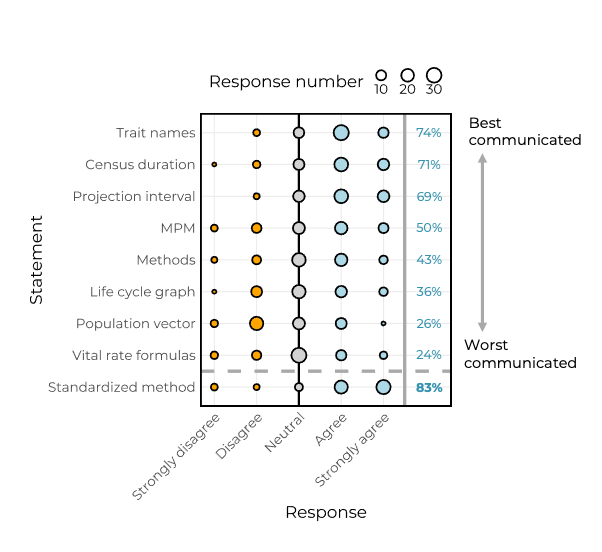
\includegraphics[keepaspectratio]{images/Survey_paper.png}}

}

\caption{FIGURA 1: Resultados de la encuesta a expertos en ecología de
poblaciones que participaron (n = 60). Los participantes calificaron su
confianza en la comunicación adecuada de los componentes de los modelos
matriciales de población (MPP) en sistemas revisados por pares. Cada
componente de MPP comunicación en el eje y representa una declaración
que se muestra en la encuesta (consulte SOM para ver la encuesta
completa). Para todas las declaraciones por encima del línea
discontinua, se preguntó a los participantes si ese atributo (por
ejemplo, intervalo de proyección) estaba suficientemente bien informado
en la publicación revisado por pares revisión. La afirmación ``método
estandarizado'' indica la respuesta de los participantes sobre si el
campo de la ecología de poblaciones se beneficiaría de un método
estandarizado de informes MPP. El tamaño de los puntos indica el número
de encuestados con esa respuesta y están coloreados (es decir, naranja =
desacuerdo; gris = neutro; azul = acuerdo). Para facilitar, el
porcentaje de acuerdo (es decir, el porcentaje de participantes que
estuvieron de acuerdo o muy de acuerdo con la afirmación) se muestra en
el lado derecho de la trama.}

\end{figure}%

2.2 \textbar{} Una muestra de publicaciones en COMPADRE y COMADRE

Para cuantificar qué tan bien se comunican los datos y metadatos de los
MPP en publicaciones revisadas por pares, seleccionamos al azar 300
artículos entre los que contenían MPP ya digitalizados en COMPADRE y
COMADRE, quedando con 150 artículos en cada caso. Entre los diferentes
atributos clave de los MPP que examinamos, hubo una variación
considerable en la confiabilidad con la que los autores proporcionaron
los datos y metadatos necesarios para digitalizar, archivar y realizar
análisis comparativos (Figura 2). Por ejemplo, la ubicación genérica de
la población examinada (i.e.~provincia/ciudad/monumento; COMPADRE:
95.1\%, COMADRE: 86.2\% de los trabajos lo reportaron), el MPP
totalmente parametrizado (93.3\%, 88.9\%) y la fecha del censo (89.6 \%,
77.7 \%) se indicaron explícitamente con frecuencia en los artículos,
mientras que la latitud y longitud de la población examinada (52.4 \%,
39.9 \%), su diagrama de ciclo de vida (44.5 \%, 40.1 \%) y el vector de
población (es decir, si la distribución por edades de los individuos en
el momento t) (33.2 \%, 32.6 \%) se indicaron con menor frecuencia.
Curiosamente, los estudios de plantas que utilizan MPP (COMPADRE)
contienen en general datos y metadatos más completos y claros que los
estudios de animales (COMADRE; Figura 2). Utilizamos esta información
para categorizar la calidad de cada uno de los 300 artículos examinados
en términos de su reproducibilidad, definida como la inclusión de los
componentes necesarios para la comunicación de los MPP (Figura 3). La
distribución de estos componentes de comunicación entre los reinos es
similar. Fundamentalmente, solo el 13.9 \% de los artículos en COMADRE y
el 15.8 \% de los artículos en COMPADRE contienen toda la información
necesaria para realizar análisis comparativos y proyecciones precisas
(Figura 3). Por lo tanto, en aproximadamente el 85 \% de los artículos
se requiere enviar un correo electrónico a los autores para solicitar la
información faltante.

\begin{figure}[H]

{\centering \pandocbounded{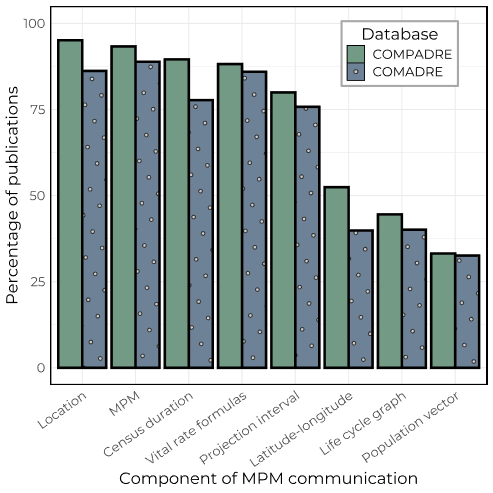
\includegraphics[keepaspectratio]{images/Database_paper.png}}

}

\caption{FIGURA2: Tanto los artículos sobre MPP de plantas como de
animales muestran patrones similares en cuanto a qué componentes
presentados de MPP se comunican. El eje y indica el porcentaje de
revisión por pares publicaciones en COMPADRE y COMADRE que contienen un
determinado atributo necesario para la comunicación clara de la
información de MPP y su reproducibilidad de un subconjunto aleatorio de
150 artículos del total de 643 artículos de COMPADRE y 150 de los 395
artículos totales de COMADRE (300 artículos en total). Los atributos
son: Ubicación: provincia/ciudad/punto de referencia; MPP: fue el MPP
incluido en el manuscrito; Duración del censo: fechas de inicio y
finalización de la recopilación de datos; Fórmulas de tasa vital:
descomposición de los elementos de la matriz en sus componentes
subyacentes (es decir, contribuciones de la supervivencia, el
crecimiento y la reproducción); Intervalo de proyección: el período de
tiempo entre observaciones; Latitud longitud: coordenadas espaciales;
Gráfico del ciclo de vida: la representación visual de la demografía.
transiciones y a/sexual per cápita contribuciones; Vector de población:
distribución st/edad de los individuos en el tiempo t asociada con la
información reportada MPP.}

\end{figure}%

\begin{figure}[H]

{\centering \pandocbounded{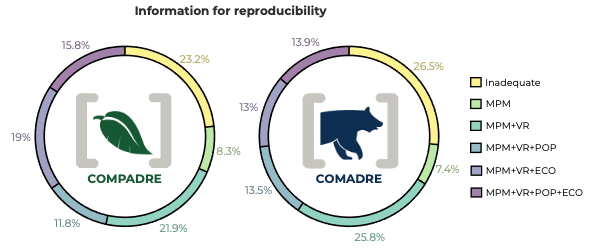
\includegraphics[keepaspectratio]{images/COMPADRE_MADRE.png}}

}

\caption{FIGURA 3: En los artículos sobre MPP de plantas y animales, la
mayoría de las publicaciones no contienen suficiente información para la
reproducibilidad. Proporción de artículos en COMPADRE y COMADRE
agrupados por su acceso abierto información en publicaciones revisado
por pares publicaciones sobre población matricial datos (MPP) y
metadatos del modelo. Siguiendo el mismo esquema que en la Figura 2, los
artículos se clasificaron en seis grupos, desde ``inadecuados'' hasta
`MPP + VR + POP+ECO' (es decir, totalmente reproducible). ``Inadecuado''
se refiere a artículos a los que les falta el MPP y/o el intervalo de
proyección (es decir, un MPP intervalo de tiempo específico necesario
para la proyección), sin el cual la mayoría de los resultados
demográficos no pueden calcularse. `MPP': el papel contiene el MPP e
intervalo de proyección, pero no hay fórmulas de tasa vital que
describan los elementos de la matriz. `MPP + VR': contiene toda la
información de `MPP' junto con fórmulas de tasa vital para los elementos
de la matriz. `MPP + VR + POP': contiene toda la información de `MPP +
VR' junto con el vector de población. `MPP + VR + ECO': contiene toda la
información para `MPP + VR' junto con la latitud y longitud coordenadas
y censo duración de la población examinada. `MPP + VR + POP + ECO':
contiene toda la información para `MPP + VR' junto con el vector de
población/ distribución, latitud-longitud coordenadas y duración del
censo.}

\end{figure}%

3 \textbar{} PROBLEMAS COMUNES CON LA CONSTRUCCIÓN DE MATRICES

Aquí, identificamos problemas clave en la parametrización de los MPP
para ilustrar el impacto de la metodología en el potencial de
extrapolación demográfica. Para hacerlo, nos basamos en los hallazgos de
la sección anterior y nuestra experiencia con la curación de COMPADRE y
COMADRE. Señalamos las siguientes cuestiones por dos razones: (i) para
guiar los demógrafos en cómo identificar estas cuestiones en la
literatura y (ii) para evitar que persistan estos problemas en futuras
publicaciones. Señalamos que una lista completa fue difundida
recientemente por {Che-Castaldo et~al.} (2020). Aquí, ampliamos estos
documentos anteriores indicando los pasos necesarios para que los
investigadores puedan evitar/mitigar estos problemas en su propia
investigación. Un resumen de estos problemas, desde la ocurrencia hasta
impacto, se detalla en la Figura S1.

3.1 \textbar{} Tipo de censo, temporalidad y frecuencia

Los MPP son modelos demográficos de tiempos medidos, parametrizados
mediante el seguimiento de individuos tras los muestreos o censos. Por
lo tanto, el tipo (p.~ej., longitudinal, transversal), el momento y la
frecuencia de los muestreos o censos deben planificarse cuidadosamente.
Estos criterios son particularmente importantes ya que el tipo de censo
afecta directamente a la construcción de la matriz, y el momento y la
frecuencia del censo pueden influir involuntariamente en los resultados
demográficos (Emery \& Gross, 2005).

Por lo general, los MPP se manejan de dos formas con respecto a la
medición de la reproducción entre censos: nacimiento-flujo o
nacimiento-pulso (ver (Caswell, 2001, p. 22)). La distinción se basa en
si la reproducción se produce de forma continua (es decir,
nacimiento-flujo) o en una estrecha ventana temporal (nacimiento-pulso).
Los MPP de nacimiento-pulso a su vez se subclasifican en censo previo
versus pos-reproductivo. Aunque tanto los censos pre-reproductivos como
los pos-reproductivos a menudo conducen a un escenario demográfico
similar (ver (Cooch, Gauthier \& Rockwell, 2003)), su diferencia radica
en la relación entre el tiempo del censo de la población y la posición
de la estrecha ventana reproductiva. En el primero, las poblaciones son
censadas inmediatamente antes de una ventana reproductiva, mientras que
los censos post-reproductivos continúan después de una ventana
reproductiva. Un censo pre-reproductivo requiere la inclusión de la
supervivencia de la descendencia en los elementos de la matriz
reproductiva, mientras que un censo post-reproductivo requiere la
inclusión de la supervivencia de los padres en los elementos de la
matriz reproductiva. A menudo encontramos errores en el acomodo de la
descendencia o la supervivencia de los padres en los elementos de la
matriz reproductiva (ver también (Kendall et~al., 2019)). Un paso clave
en la construcción de la matriz que puede evitar el acomodo incorrecto
de la supervivencia sería dibujar el gráfico del ciclo de vida (según
({Ebert}, 1999, p. 61)) con respecto al momento del censo (demostrado en
({Ellner et~al.}, 2016, p. 13)), así como también detallar
explícitamente el tipo de censo utilizado para parametrizar el MPP. Sin
embargo, a veces dibujar el gráfico del ciclo de vida puede que sea
inviable o poco informativo. Por ejemplo, el gráfico de un modelo
clasificado por edad si tuviera 100 clases de edad sería demasiado
grande para dibujarlo y no muy útil; sin embargo, se podría simplificar
con una línea discontinua si varias clases adyacentes tienen las mismas
tasas demográficas (por ejemplo, ({Ebert}, 1999, p. 2)). Los modelos con
muchas etapas y transiciones altamente conectadas no son viables para
dibujar el gráfico del ciclo de vida (por ejemplo, el gráfico de
\emph{Calathea ovandensis} en (Neubert \& Caswell, 2000)). Pero incluso
en situaciones complejas (por ejemplo, la serie de gráficos estacionales
para el pingüino emperador en (Jenouvrier et~al., 2010)), el gráfico
puede ser útil para organizar la estructura del modelo. El tiempo y la
frecuencia del censo afectan la construcción del modelo, lo que hace que
un MPP construido no sea práctico para la inferencia demográfica si no
se considera la historia de vida del organismo examinado. Considere a un
investigador que compara los procesos demográficos de las moscas de la
fruta y los árboles frutales. El investigador primero nota que hay
cuatro etapas discretas en la historia de vida de las moscas de la
fruta: tres etapas juveniles que abarcan el desarrollo desde el huevo
hasta el estadio y la pupa, y una etapa adulta donde los individuos se
dispersan y reproducen. Dado que el desarrollo de huevo a adulto tarda
\textasciitilde10 días en esta especie, el investigador decide realizar
el censo cada 10 días tanto para la mosca de la fruta como para los
árboles frutales durante un período de 3 meses. Sin embargo, debido a
que ni la mortalidad ni la reproducción ocurren en un censo tan corto en
la población de árboles frutales, el MPP de árboles frutales resultante,
cuando se proyecta hacia adelante, persistirá para siempre, sin aumentar
ni disminuir. Este mismo problema ocurriría al revés. Si los intervalos
de 5 años se consideraran suficientes para los árboles frutales, las
moscas de la fruta medidas individualmente nunca sobrevivirían a lo
largo de los períodos de tiempo. Existe una solución a este problema,
utilizando modelos de matrices periódicas para incluir períodos mucho
más cortos o más largo que otros períodos. Por ejemplo, (Hunter et~al.,
2010) analizaron la pardela negra \emph{Puffinus griseus} incluyendo dos
períodos de cosecha de varias semanas de duración y luego un intervalo
anual para la especie, con una vida útil de décadas. (Smith, Caswell \&
Mettler-Cherry, 2005) y (Shyu et~al., 2013) utilizaron modelos
estacionales periódicos para adaptarse a los ciclos de vida en los que
algunas etapas solo están presentes durante una parte del ciclo anual.
El enfoque (Caswell, 2001, sec. 13.1) es poderoso y general.

3.2 \textbar{} Supervivencia etapa-específica poco realista

Los problemas en la parametrización de la supervivencia
etapa-específica, si bien son fáciles de diagnosticar, son difíciles de
controlar y pueden dar lugar a una variedad de historias de vida no
naturales. Las probabilidades de transición y supervivencia están
limitadas entre 0 (el evento nunca sucede) y 1 (el evento siempre
ocurre). Es evidente que, considerando la etapa-específica supervivencia
de un MPP, los elementos no reproductivos sumados en una columna dada
del MPP A no deben exceder 1. Cuando lo hace, los individuos en esa
etapa tienen una probabilidad poco realista de sobrevivir
\textgreater100\%, lo que resulta en una representación incorrecta de la
historia de vida del organismo. Los valores de \textgreater1 de
supervivencia etapa-específica generalmente surgen debido a errores de
redondeo, errores tipográficos, e inclusión de eventos reproductivos
a/sexuales no declarados y generalmente se recomienda omitir estos MPP
en un análisis comparativo ({Jones et~al.}, 2014). Los eventos
reproductivos a/sexuales no declarados ocurren cuando un elemento
\(a_{i,j}\) en el MPP \(A\) combina procesos dependientes de la
supervivencia, como el crecimiento/encogimiento, pero también la
fertilidad, y que estos no se han informado por separado. De
preferencia, los autores identificarían cuidadosamente si varias tasas
vitales se confunden con procesos demográficos dependientes de la
supervivencia en cada elemento del MPP. Para el demógrafo comparativo
que utiliza COMPADRE y COMADRE, recomendamos evitar los modelos MPP
donde supervivencia etapa-específica llega a ser \textgreater1, y
también evitar alterar el modelo para hacer que la supervivencia
etapa-específica se fije a un máximo de 1 (p.~ej., (Buckley et~al.,
2010)). En muchos MPP publicados, algunas de las etapas de la vida
tienen un tiempo estimado probabilidad de supervivencia de 1 o un ciclo
de vida incompleto, probablemente el resultado de un tamaño de muestra
pequeño o algún evento raro a lo largo de la historia de vida del
especies. La supervivencia perfecta (es decir, mortalidad = 0) es poco
probable y es posible que el valor deba estimarse o imputarse ({Johnson
et~al.}, 2018). Un método para estimar valores realistas de
supervivencia y transición fue propuesto recientemente por (Tremblay
et~al., 2021), utilizando un enfoque bayesiano para estimar los valores
de los parámetros utilizando datos previos, además de los datos
observados, para obtener los MPP. Una ventaja de este enfoque es que los
intervalos de confianza de los parámetros que representan probabilidades
(estasis, transición, supervivencia) se obtienen a partir de una
distribución beta. La ventaja de usar una distribución de Dirichlet
multinomial bayesiana inferida para estimar los valores medios es que
los investigadores pueden inferir la varianza y el sesgo de las
distribuciones posteriores para informar mejor la construcción de MPP y
la interpretación demográfica (p.~ej., Tremblay et~al. (2009a). Por
último, dado que el tamaño de la muestra puede ser un factor causante de
la supervivencia etapa-específica poco realista, el tamaño de la muestra
y la incertidumbre (p.~ej., intervalo de confianza, desviación estándar)
deben informarse para (1) transmitir la precisión de los valores
estimados de supervivencia y (2) para la inclusión precisa de los
valores de supervivencia en metaanálisis y métodos comparativos.

3.3 \textbar{} Parametrización incorrecta de la fertilidad

La fertilidad a menudo presenta un desafío para la construcción de MPP
precisos. Este desafío se debe en parte a la ambigüedad del término
``fertilidad''. El problema surge cuando las contribuciones individuales
(per-cápita) de los adultos reproductivos a los nuevos reclutas (por
ejemplo, huevos, neonatos, semillas, etc.) no representan los enlaces
que contempla el intervalo de proyección completo del estudio. Recuerda
que la entrada \(a_{i,j}\) en un MPP es el número (esperado) de
individuos en etapa \(i\) en \(t + 1\) por estadio \(j\) individuo en el
tiempo \(t\). Si la etapa \(i\) es efectivamente un tipo de individuo
`recién nacido', entonces \(a_{i,j}\) debe incluir todos los procesos
entre tiempo \(t\) y tiempo \(t + 1\) (Caswell, 2001), p.~61).
Rendimiento reproductivo, a su vez, es un proceso demográfico compuesto
del número de descendientes producidos en un evento reproductivo y la
supervivencia pertinente que penalizará en cuanto al número de
descendientes nuevos que alcanzarán a la siguiente observación. El no
tener en cuenta esta descomposición de la tasa vital puede resultar en
la introducción de un retraso por una unidad de tiempo (en los términos
del caso particular) en el ciclo de vida del organismo, ya que la
descendencia recién creada pasaría un intervalo de proyección 'en limbo
'antes de su transiciones hacia delante. El ejemplo más conocido está en
el modelo clásico del cardo \emph{Dipsacus sylvestris}, de (Werner \&
Caswell, 1977), en el que las plantas con flores en el momento \(t\),
pasaron a tener semillas en el tiempo \(t + 1\), y que éstas solo
germinaron para formar plántulas en el tiempo \(t + 2\). Este tema fue
discutido y corregido en (Caswell, 2001). Además, este problema se ha
reportado, por ejemplo, en estructuras reproductivas, tales como
semillas, que no forman parte de un banco de semillas. Si se presenta
este tipo de problema en un MPP, generalmente {[}Kendall et~al. (2019),
pero no siempre (Nguyen et~al., 2019), se subestima la tasa de
crecimiento γ de la población asintótica, y de allí se enfrenta el
desafío de estimar la importancia relativa del banco de semillas y la
vida útil de estas semillas aun no germinadas. El efecto de parametrizar
incorrectamente la fertilidad dentro de la tasa de crecimiento γ es
mayor en casos de crecimiento extremo, por ejemplo, en especies
invasoras, o, al contrario, disminución extrema, como la que observamos
en especies en peligro de extinción crítico (Steiner, Tuljapurkar \&
Roach, 2021). Este fenómeno también puede causar una sobre-estimación de
la envoltura transitoria (ver Ezard et~al., 2010). Por ello,
recomendamos especificar las fórmulas de la tasa vital de fecundidad en
conjunto con los MPP asociados e identificar claramente los valores de
estas tasas vitales subyacentes (como en el Recuadro 1).

3.4 \textbar{} Cálculo indirecto de tasas vitales

La estimación de las tasas vitales a menudo implica una combinación de
medidas directas e indirectas. La medición directa deriva empíricamente
las tasas vitales a partir de datos basados en individuos, donde se
censan los mismos individuos etiquetados varias veces, como en los
estudios de tablas de vida de cohortes, métodos de
captura-marcado-recaptura y muchos estudios de cuadrantes de plantas
marcadas. Sin embargo, las tasas vitales pueden ser difíciles de
observar en especies con altas tasas de reproducción, fenología compleja
y/o poblaciones pequeñas (Beissinger \& Westphal, 1998). En
consecuencia, las estimaciones de reclutamiento a menudo se usan para
complementar los MPP desarrollados en condiciones controladas, por
ejemplo, en el laboratorio {[}Jouvet, Rodrı́guez-Rojas \& Steiner
(2018)), en un invernadero (Gontijo \& Carvalho, 2020), en un zoológico
(Clubb et~al., 2009) o en un jardín botánico (Jiménez-Valdés et~al.,
2010). Dado que algunos métodos para el desarrollo de los MPP requieren
de un ciclo de vida completo para obtener las métricas clave (por
ejemplo, métricas transitorias: Stott, Townley \& Hodgson, 2011), se
tiende a utilizar sitios de estudio externos o fuentes de la literatura
para parametrizar los componentes que hacen falta para `cerrar el ciclo'
(Omeyer et~al., 2021). Sin embargo, hay que tomar en cuenta que las
poblaciones cautivas o de alguna forma domesticadas pueden no presentar
la misma dinámica poblacional que la población natural (Clubb \& Mason,
2003), particularmente en relación a supervivencia (Che-Castaldo et~al.,
2021) o reproducción (Clubb et~al., 2009).

Otro método para estimar indirectamente las tasas vitales consiste en
utilizar métodos ex situ para obtener los límites superior e inferior
del reclutamiento (u otras tasas vitales) y explorar los espacios
ocupados por los parámetros dentro de esos límites. Este enfoque fue
introducido por (Caswell et~al., 1998) en un estudio sobre los efectos
de la mortalidad por captura incidental en la marsopa común. Los
cronogramas de supervivencia y fertilidad específicos por edad se
seleccionaron de otras especies con ciclos de vida similares, se
reajustaron para que coincidieran con la longevidad de la marsopa común
y se usaron para producir distribuciones de incertidumbre para el
crecimiento de la población y los efectos de la captura incidental
medida. La información así generada de la distribución y los parámetros
asociados proporciona una medida de incertidumbre a partir de la cual
informar la construcción de un MPP (Tenhumberg et~al., 2008). Además, el
uso de la jerarquía en los modelos para estimar los valores faltantes y
la fuerza de préstamo de otras poblaciones o especies pueden mejorar la
estimación de los parámetros (Tremblay \& McCarthy, 2014; James et~al.,
2021).

Por último, los modelos poblacionales integrados representan un marco
valioso para estimar indirectamente las tasas demográficas y la dinámica
de la población (tamaño y estructura) mediante la combinación de fuentes
de datos, en particular la combinación de datos individuales
longitudinales con datos de censos poblacionales (Plard et~al., 2019;
Schaub \& Kéry, 2021). Los modelos de población integrados permiten la
construcción de modelos de población (incluyendo los MPP) mediante, (1)
la combinación de diversas fuentes de datos, (2) la definición de una
historia de vida a priori (a menudo se trata de algún tipo de modelo de
población estructurado por etapas) y (3) la cuantificación de la máxima
probabilidad de las tasas demográficas codificadas en la historia de
vida, y citando las fuentes de los datos. Los modelos de población
integrados son particularmente útiles cuando se conoce la incertidumbre
en torno a la adquisición de datos (por ejemplo, en estudios de
captura-marcado-recaptura) (Riecke et~al., 2019).

3.5 \textbar{} Vector de población

Una estimación de la estructura de la población, clasificada por edad o
etapa, es una pieza útil de información cuando está disponible, pero no
siempre se cuenta con esta información. Tiene lógica utilizar la
estructura actual de la población como punto de partida para las
proyecciones de la viabilidad de la población a corto y largo plazo
(Werner \& Peacock, 2019). Además, el utilizar la población vector (es
decir, abundancia y distribución de etapas) para las proyecciones ayuda
para tener en cuenta los efectos de la dinámica transitoria, que mide el
efecto de la estructura de población no estacionaria en tasas de
crecimiento de ``near term'' de las poblaciones (Capdevila et~al.,
2020). Los vectores reportados de etapa o edad de la población reflejan
dos componentes clave: la estructura de población real en el censo en el
tiempo t y las opciones metodológicas. Este segundo componente es
fundamental para representar con precisión la población estudiada.

A través del desarrollo y curación de COMPADRE y COMADRE, hemos notado
dos fuentes de error que afectan la estimación de los vectores de
población. El primer error es un sesgo de detección, donde los
investigadores identifican ciertas etapas/edades con una mayor tasa de
detección que las etapas más crípticas (por ejemplo, plantas adultas
versus bancos de semillas). El segundo error es la apropiación indebida
de los métodos utilizados para cuantificar las tasas demográficas como
base para estimar la abundancia de etapa. Este segundo error proviene de
un malentendido de la diferencia entre estimar tasas y estimar números.
Para medir las tasas demográficas, durante un censo, los investigadores
a veces aumentan el esfuerzo de muestreo de ciertas clases de etapa/edad
en relación a otras. Este diferencia en el esfuerzo en relación a
etapa/edad es particularmente común cuando las clases de etapas/edades
tienen probabilidades de supervivencia cercanas a sus límites (es decir,
0 y 1). Por ejemplo, en la demografía de los árboles, normalmente solo
hay unos pocos individuos muy grandes por área examinada. Por lo tanto,
a menudo los investigadores complementan el tamaño de la muestra de esta
categoría al muestrear fuera del área predefinida (Jones \& Hubbell,
2006). Sin embargo, muchos métodos para la estimación de tasas
demográficas no proporcionan ninguna información sobre números y
estructura de la población. Las tablas de vida de cohortes, que siguen a
una cohorte de individuos a medida que envejecen, son ciegos a la
estructura de la población en la que se desarrolla la cohorte. De hecho,
puede que no haya tal población (por ejemplo, toda la historia de
demografía basado en el estudio de cohortes realizada en laboratorio,
que se remonta a Pearl en la década de 1920 (Pearl, Miner \& Parker,
1927). La estimación de tasas mediante la técnica de
captura-marcar-recaptura a partir de datos longitudinales extrae toda su
inferencia de los individuos marcados y en ningún momento hace
referencia al número y la estructura de los no marcados. La literatura
sobre métodos de captura-marcar-recaptura para la estimación de tasas
reconoce que estimar el tamaño de la población es mucho más difícil que
estimar las tasas (Lebreton et~al., 1992) y requiere diferentes modelos
de captura-marcar-recaptura (por ejemplo, la inclusión de la evaluación
de la respuesta hacía las trampas (dispuesto / renuente) en la
estimación de tasas vitales.

CAJA 1: Ejemplo de presentación de un hipotético sistema de tres etapas
de modelo de población de matriz de una planta (MPP) usando una
presentación explícita de datos aplicables a la mayoría de las técnicas
de construcción MPP.

\begin{enumerate}
\def\labelenumi{(\Alph{enumi})}
\tightlist
\item
  Tipo de matriz
\end{enumerate}

Una matriz simple determinista y independiente de la densidad.*

*Este campo de texto libre permite la breve descripción del tipo de
matriz. Si la matriz está estructurada por una variable, la matriz es
simple. Si en caso contrario, la matriz se considera general (por
ejemplo, edad x etapa). Determinista se refiere a si las tasas
demográficas que construyen el MPP se mantienen constantes
(determinista) o extraídas de una distribución (estocástica).
Independiente de la densidad versus dependiente de la densidad indica si
las tasas demográficas están o no influenciadas por la densidad de
población.

\begin{enumerate}
\def\labelenumi{(\Alph{enumi})}
\setcounter{enumi}{1}
\tightlist
\item
  Diagrama de ciclo de vida
\end{enumerate}

\pandocbounded{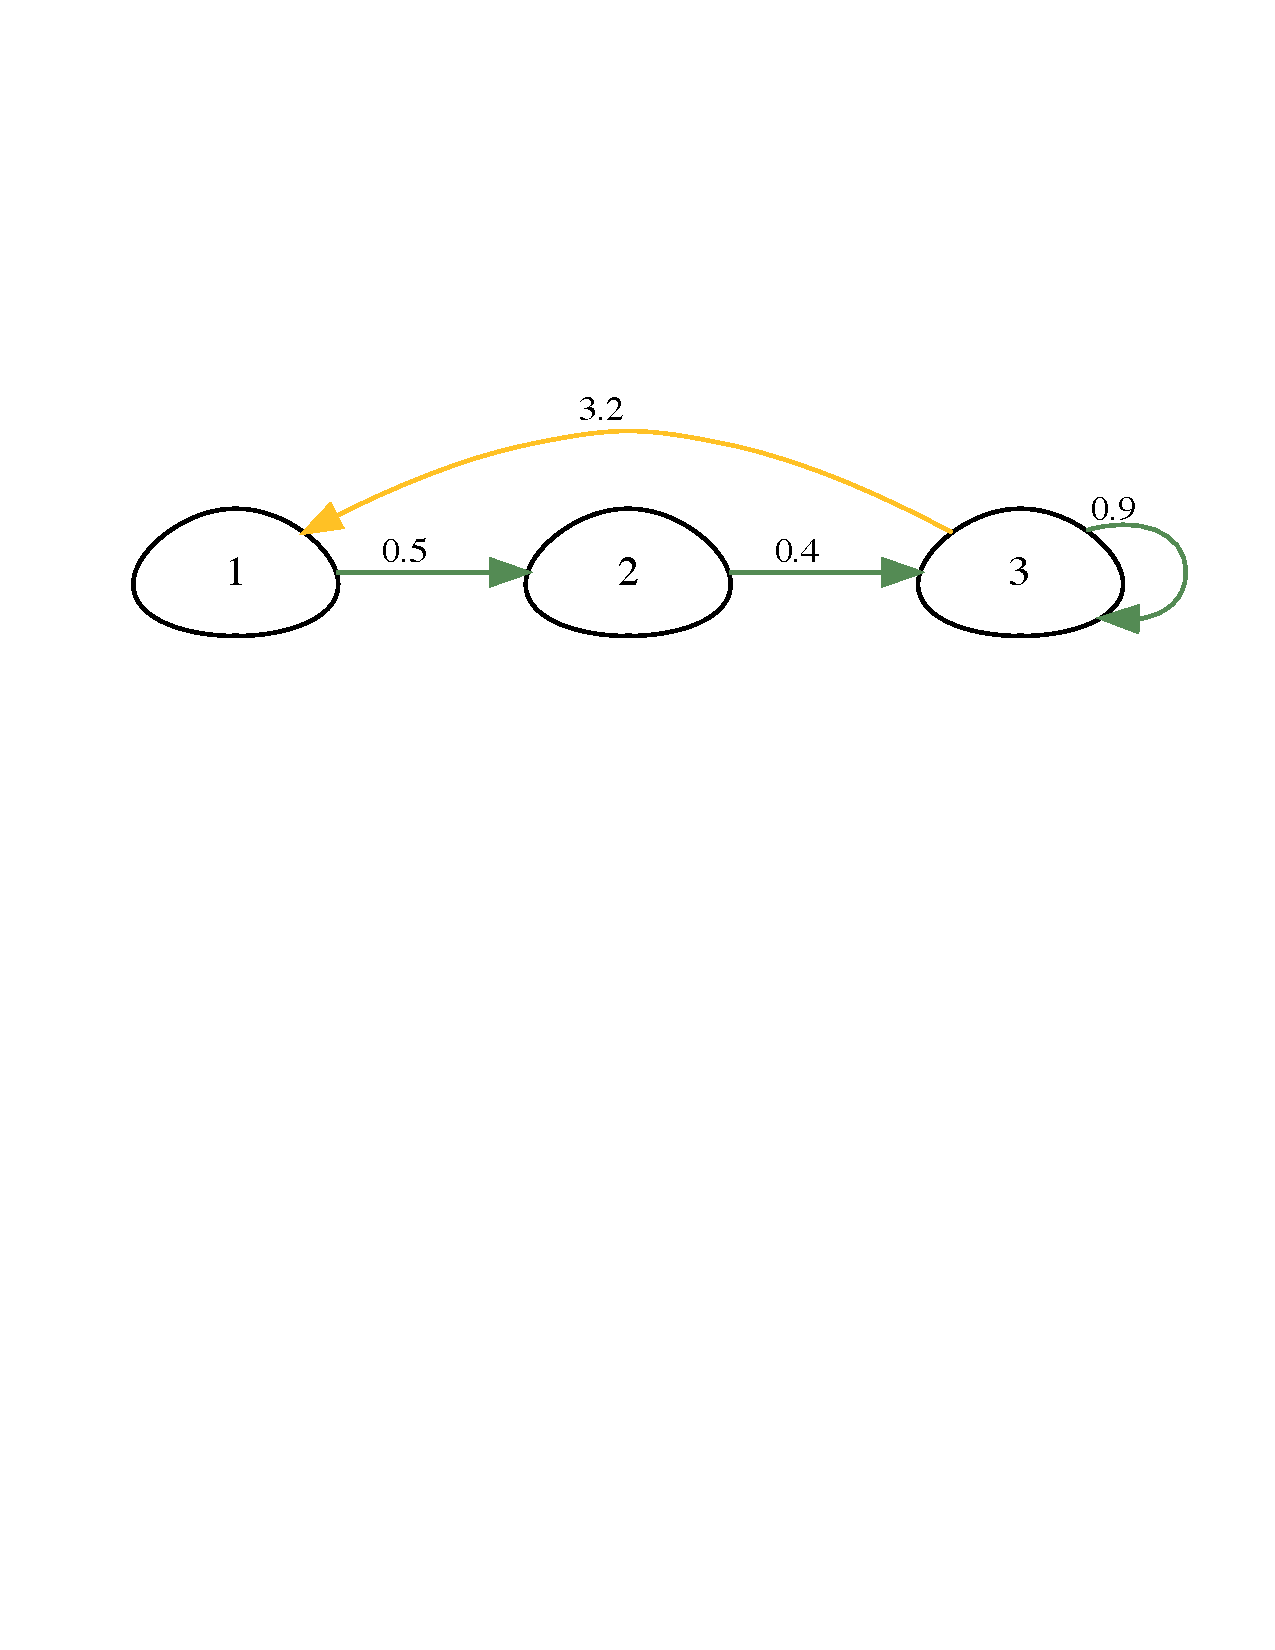
\includegraphics[keepaspectratio]{121-Traduccion_protocolo_informacion_files/figure-pdf/Proto1-1.pdf}}

\begin{center}\rule{0.5\linewidth}{0.5pt}\end{center}

\begin{enumerate}
\def\labelenumi{(\alph{enumi})}
\setcounter{enumi}{2}
\tightlist
\item
  Descripción del Censo
\end{enumerate}

\begin{verbatim}
Error in `italic()`:
! could not find function "italic"
\end{verbatim}

\begin{center}\rule{0.5\linewidth}{0.5pt}\end{center}

\begin{enumerate}
\def\labelenumi{(\Alph{enumi})}
\setcounter{enumi}{3}
\tightlist
\item
  Nombres de las etapas y clasificación
\end{enumerate}

\begin{verbatim}
Error in `align()`:
! could not find function "align"
\end{verbatim}

\begin{center}\rule{0.5\linewidth}{0.5pt}\end{center}

\begin{enumerate}
\def\labelenumi{(\Alph{enumi})}
\setcounter{enumi}{4}
\tightlist
\item
  Definiciones de las Tasas vitales
\end{enumerate}

{\def\LTcaptype{none} % do not increment counter
\begin{longtable}[]{@{}
  >{\raggedright\arraybackslash}p{(\linewidth - 4\tabcolsep) * \real{0.0803}}
  >{\raggedright\arraybackslash}p{(\linewidth - 4\tabcolsep) * \real{0.7226}}
  >{\raggedright\arraybackslash}p{(\linewidth - 4\tabcolsep) * \real{0.1971}}@{}}
\toprule\noalign{}
\begin{minipage}[b]{\linewidth}\raggedright
Tasa Vital
\end{minipage} & \begin{minipage}[b]{\linewidth}\raggedright
Definición
\end{minipage} & \begin{minipage}[b]{\linewidth}\raggedright
Procedencia de los valores
\end{minipage} \\
\midrule\noalign{}
\endhead
\bottomrule\noalign{}
\endlastfoot
\(S_{ij}\) & Supervivencia de la etapa \emph{j} a la etapa \emph{i} &
Datos de campo \\
\(N_{s}\) & Número de semillas por fruto & Datos de campo \\
\(N_{fx}\) & Número de frutos producido por un individuo en el tamaño de
categoría \emph{x} & Datos de campo \\
\(P_{rx}\) & La probabilidad de reproducción de un adulto en la
categoría \emph{x} & Datos de campo \\
\(P_{s}\) & Probabilidad de germinación de semillas y supervivencia de
plántulas en el intervalo de proyección & Datos de Invernadero \\
\end{longtable}
}

\begin{enumerate}
\def\labelenumi{(\Alph{enumi})}
\setcounter{enumi}{5}
\tightlist
\item
  Valores de las razones de transición vitales
\end{enumerate}

{\def\LTcaptype{none} % do not increment counter
\begin{longtable}[]{@{}
  >{\raggedright\arraybackslash}p{(\linewidth - 6\tabcolsep) * \real{0.2192}}
  >{\raggedleft\arraybackslash}p{(\linewidth - 6\tabcolsep) * \real{0.2192}}
  >{\raggedleft\arraybackslash}p{(\linewidth - 6\tabcolsep) * \real{0.2329}}
  >{\raggedleft\arraybackslash}p{(\linewidth - 6\tabcolsep) * \real{0.3288}}@{}}
\toprule\noalign{}
\begin{minipage}[b]{\linewidth}\raggedright
Etapas Vitales
\end{minipage} & \begin{minipage}[b]{\linewidth}\raggedleft
Estimados*
\end{minipage} & \begin{minipage}[b]{\linewidth}\raggedleft
Error Estándar**
\end{minipage} & \begin{minipage}[b]{\linewidth}\raggedleft
Tamaño de muestra (N)***
\end{minipage} \\
\midrule\noalign{}
\endhead
\bottomrule\noalign{}
\endlastfoot
\(S_{21}\) & 0.400 & 0.100 & 80 \\
\(S_{32}\) & 0.850 & 0.050 & 160 \\
\(S_{33}\) & 0.900 & 0.020 & 160 \\
\(N_{s}\) & 1000 & 150 & 80 \\
\(N_{f3}\) & 2.000 & 300 & 80 \\
\(P_{r3}\) & 0.300 & 0.040 & 200 \\
\(P_{s}\) & 0.005 & 0.001 & 500 \\
\end{longtable}
}

*Si estas estimaciones dependen del tamaño de la población (es decir,
dependencia de la densidad) o en respuesta a una variable ambiental (es
decir, ambiental, estocasticidad), la estimación debe comunicarse como
una función (por ejemplo,
\(S_{33}\sim\ 0,9\ +\ \beta_{precipitacion}\ \cdot\ 0,01\) donde la
precipitación ∼ N(5, 1)). Además, si se trata de una estimación puntual,
los investigadores deben indicar si los valores representan valores
medios o medianos.

**Esta medida de incertidumbre también puede ser la desviación estándar,
la varianza o un intervalo de confianza/creíble de la estimación, a
discreción. del investigador.

***Indique si la unidad de medida/replicación es a nivel de organismos
individuales o a nivel de grupos (por ejemplo, cohortes, colonias,
familias).

\begin{center}\rule{0.5\linewidth}{0.5pt}\end{center}

\begin{enumerate}
\def\labelenumi{(\Alph{enumi})}
\setcounter{enumi}{6}
\tightlist
\item
  Fórmula MPP (Mayo 2021 a Mayo 2022)
\end{enumerate}

{\def\LTcaptype{none} % do not increment counter
\begin{longtable}[]{@{}lll@{}}
\toprule\noalign{}
Plántulas & Rosetas & Adultos \\
\midrule\noalign{}
\endhead
\bottomrule\noalign{}
\endlastfoot
0 & 0 & \(N_{s}*N_{f3}*P_{r3}*P{s}\) \\
\(S_{21}\) & 0 & 0 \\
0 & \(S_{32}\) & \(S_{33}\) \\
\end{longtable}
}

\begin{enumerate}
\def\labelenumi{(\Alph{enumi})}
\setcounter{enumi}{7}
\tightlist
\item
  Vector de la población (Mayo 2021)
\end{enumerate}

\begin{verbatim}
Error in `flextable()`:
! could not find function "flextable"
\end{verbatim}

*Esta medida de incertidumbre también puede ser la desviación estándar
de la estimación, la varianza o un intervalo de confianza/creíble a
discreción. del investigador.

3.6 \textbar{} Omitir etapas de vida crípticas

La identificación y estimación de tasas vitales en etapas crípticas
representa un reto en ecología de poblaciones. Se determinan las etapas
crípticas como puntos a lo largo del ciclo de vida de un organismo que
están, de una forma u otra, ocultos o se pasan por alto por ecologistas
de poblaciones al construir modelos de población (Doak, Diane Thomson \&
Jules, 2002). Una etapa de la vida puede ser críptica porque es
logísticamente difícil de observar, o, aunque si es observable, a su vez
es indistinguible de otra etapa (Nguyen et~al., 2019). En las plantas,
etapas crípticas pueden surgir de los bancos de semillas, como en el
caso de las orquídeas, donde las semillas son demasiado pequeñas para
ser observadas e identificadas en el campo (Paniw et~al., 2017) o
algunas perennes herbáceas (por ejemplo, \emph{Astragalus scaphoides})
donde períodos de latencia vegetativa permiten que los individuos
permanezcan escondidos bajo tierra durante una o más temporadas de
crecimiento (Gremer \& Sala, 2013). Además, los animales pueden exhibir
etapas crípticas al pasar por diapausa o retrasos en el desarrollo
debido a condiciones ambientales adversas (p.~ej. \emph{Aedes
albopictus}: (Jia et~al., 2016)). Aves marinas pelágicas (albatros,
petreles, pingüinos) a menudo pasan etapas pre-reproductivas en el mar,
a veces de duraciones de muchos años, y al ser así, se mantienen
completamente crípticas hasta volver a la colonia reproductora como
adultos. Métodos sofisticados de marcado-recaptura multi-estado pueden
proporcionar estimaciones de parámetros para estas partes del ciclo de
vida Choquet, Rouan \& Pradel (2009). Omitir una etapa críptica de la
vida puede reducir el realismo biológico de un MPP y alterar el número
de etapas en el MPP, que, en su conjunto puede impactar aún más los
resultados demográficos (Tenhumberg, Tyre \& Rebarber, 2009;
Salguero-Gómez \& Plotkin, 2010). En algunos casos, las etapas de la
vida crípticas solo se identificarán a través de un enfoque
multidisciplinario. incluyendo métodos de campo y de laboratorio, junto
con marcos bayesianos para integrar datos y conocimientos previos (por
ejemplo, Paniw et~al., 2017).

3.7 \textbar{} Modelos de uno versus dos sexos

Gran parte de la demografía se centra en las hembras, bajo los supuestos
que la fertilidad está determinada por las hembras sin limitación por
los machos (ver Caswell, 2001, p. 568). Dichos modelos pueden incluir
machos (por ejemplo, Hunter et~al., 2010), pero si la reproducción está
determinada por las tasas femeninas (es decir, dominado por la etapa de
hembras). Los machos representan un conjunto de etapas que no
contribuyen al crecimiento de la población. La mayoría de los MPP de
animales existentes están a base de hembras y femenino dominante
({Salguero-Gómez et~al.}, 2016) dados sesgos de muestreo hacia mamíferos
y aves ({Conde et~al.}, 2019), a menudo no es factible, o necesario para
la pregunta de investigación, rastrear interacciones reproductivas
masculinas (Archer et~al., 2022). Estos estudios, por lo general, asumen
una proporción de sexos 1:1, y las tasas vitales son congruente por sexo
y la reproducción no es limitada por los machos de la especie
(Compagnoni, Steigman \& Miller, 2017; Miller \& Compagnoni, 2022).
Mientras que un sexo los modelos son comunes en animales MPP'S
(actualmente 77\% en Comadre v. 4.21.8), se debe tener cuidado no hacer
suposiciones sobre la relación sexual dinámica dependiente dentro estos
sistemas (Archer et~al., 2022). De hecho, estos supuestos no pueden ser
cumplido cuando cualquiera de los siguientes es cierto: que haya un
sesgo en la proporción de sexos (Archer et~al., 2022), hay reproducción
sesgadas (Sky et~al., 2022), o un alta sensibilidad de la dinámica de la
población en respuesta a la elección de apareamiento (Veran \&
Beissinger, 2009). Además, la detectabilidad de los diferentes sexos en
el muestreo dependiente del sexo puede confundir más las estimaciones de
la relación sexual y sus impactos asociados sobre las tasas vitales si
no se tiene en cuenta. Los modelos de dos sexos que no asumen la
dominancia por un sexo no son lineales y requiere especificaciones de
una función de apareamiento que describe la fertilidad en función del
macho y la abundancia hembras (Caswell, 2001). La definición de tales
funciones de apareamiento es generalmente difícil o imposible, excepto
en casos específicos como la estricta monogamia (Jenouvrier et~al.,
2010).

Informar sobre las proporciones de sexos puede expandir enormemente el
alcance de un estudio Shyu \& Caswell (2016b); Por ejemplo, evaluar el
impacto de la razón de sexo cuando hay efecto Allee (Boukal \& Berec,
2002). Desafortunadamente, este tipo de análisis es raro y pocos
ejemplos son notados en las bases de datos de COMPADRE y COMADRE.
Además, si hay diferencias en los valores de la tasa vital entre sexos,
como supervivencia, crecimiento y/o producción reproductiva en los
modelos basados en un sexo solamente los MPP pueden omitir procesos
importantes (Caswell, 2001, p. 568; Archer et~al., 2022). En plantas,
ejemplos de investigaciones que incluye la dinámica de dos sexos raro
(0.2\% en COMPADRE v. 6.22.5). Este bajo porcentaje probablemente
refleja en parte la rareza de las plantas dioicas u otros sistemas de
apareamiento con dos o más sexos ({Gabriel, John, et~al.}, 2017) y los
sistemas de apareamiento polígamos que hacen que la reproducción y la
dinámica poblacional limitada a los machos sea rara (ver Compagnoni,
Steigman \& Miller, 2017; Miller \& Compagnoni, 2022).

3.8 \textbar{} Irreductibilidad y ergodicidad

Las propiedades de la irreductibilidad tienen implicaciones sobre la
diversidad de eigenvalue de una matriz y, por lo tanto, interpretaciones
biológicamente relevantes (e.g.~tasas de crecimiento de la población,
estructuras de etapa estable). Estas implicaciones son bien conocidos en
la literatura sobre MPP (Caswell, 2001). Matrices que son irreducibles
son aquellas en las que el gráfico del ciclo de vida está completamente
conectado; es decir, existe una ruta directa o indirecta desde cualquier
etapa a cualquier otra etapa. A veces se afirma que los MPP reducibles
son de alguna manera inválido; ellos no son inválido. Hay (al menos)
cuatro situaciones en que matrices reducibles ocurren naturalmente.

Ciclos de vida con etapas post-reproductivas. Las etapas
post-reproductivas no pueden contribuir a las potencialmente
reproductivas (por ejemplo, MPP's para humanos, Orcas).

Modelos de dos sexos dominados por un sexo (generalmente mujeres, pero
podría ser hombre). En un modelo dominado por hembras, toda la
reproducción es acreditado a las mujeres. Los machos son producidos por
las hembras, pero los machos no hacen contribución a la parte femenina
del ciclo de vida por ejemplo, (Hunter et~al., 2010) para osos polares).

Modelos espaciales en los que la dispersión es unidireccional, como en
los sistemas fluviales (ríos) o corrientes oceánicas.

En los modelos de Edad × Etapas (Caswell, 2009; Caswell \&
Salguero-Gómez, 2013). En estos modelos, la reproducción produce (por
definición) individuos en la clase de edad 1, pero el modelo incluye
todas las combinaciones de edad y etapa, incluidas combinaciones
imposibles de edad de clase 1 y etapas que no existen a los 1 años.

La reductibilidad puede o no ser fácil de detectar desde el gráfico del
ciclo de vida, pero se puede evaluar numéricamente. La matriz A es
irreducible si y solo si la matriz \(\left(I+A\right)^{s-1}\) es
positiva (Caswell, 2001). La irreductibilidad, junto con la
primitividad, es una condición suficiente para Ergodicidad, garantizando
que la población convergerá a la misma estructura estable
independientemente de la condición inicial. Una matriz reducible puede
no tener esta propiedad; claramente, por ejemplo, si una población
comenzó con un solo individuo post-reproductivo no convergerá a la misma
estructura que una que comenzó con algunos individuos pre-reproductivos.
Con respecto a la ergodicidad, también se sabe que un MPP es ergódico si
y solo si todas las entradas de su vector propio dominante izquierdo (v)
son positivas (Stott et~al., 2010b). En resumen, a pesar del modelo
apropiado estructura y parametrización correcta, los datos demográficos
pueden conducir a matrices reducibles y/o no ergódico.

4 \textbar{} Representación completa de un MPP en publicaciones

En esta sección, justificamos la necesidad de una presentación clara de
MPP's en la literatura científica, sugerencias dónde archivar los MPP's
en base da datos de acceso abierto, y discutir cómo estas dos acciones
benefician a los autores, revistas editoriales, lectores, demógrafos
comparativos, meta-analistas y la disciplina en general. Una tabla que
contiene la lista de los datos a incluir al publicar MPP's junto con una
justificación para la inclusión. Se pueden encontrar ejemplos de buenas
prácticas en Tabla S1.

4.1 \textbar{} Partición de los procesos demográficos

Es importante definir a qué se refiere cada elemento de una matriz de un
MPP's. Varios procesos demográficos pueden superponerse al mismo
elemento matriz en un MPP, particularmente en especies con un rápido y/o
variable ciclo de vida relativo a los intervalos de proyección del MPP.
Por ejemplo, el parámetro en un MPP que representa el enlace entre
individuos grandes en el tiempo \(t\) y individuos más pequeños en el
tiempo \(t+1\) podría corresponder a la reproducción sexual,
reproducción clonal, fisión, retroceso o un conjunto de los procesos
anteriores. Las derivaciones matemáticas de parámetros clave de la
historia de vida (por ejemplo, generación el tiempo, la esperanza de
vida, la tasa de senescencia, el grado de iteroparidad) requieren que
estos procesos estén claramente separados ({Jones et~al.}, 2022). Esta
separación es crítica para la familia de análisis basados en las cadenas
de Markov; la matriz U define las transiciones de estado transitorio en
un análisis de cadena de Markov absorbente (Caswell, 2011; Caswell \&
Salguero-Gómez, 2013). Claramente describiendo la estructura subyacente
de las tasas demográficas en un diagrama del ciclo de vida y su
consecuente modelo de población de la matriz completa A, se pueden
separar las matrices en los procesos de supervivencia (por ejemplo,
progresión/crecimiento, retroceso/ contracción, fisión, fusión, estasis)
en la submatriz U, una matriz de reproducción sexual en el submatriz F y
la reproducción clonal en la submatriz C (Figura 4). Es importante
destacar que tanto las matrices F y C incluyen elementos que deben
incorporar la supervivencia de acuerdo con el tipo de censo (es decir,
pre-/post-reproductivo censo).

Informando claramente la matriz A y las submatrices U, F y C se lleva
dos beneficios clave: (1) indica explícitamente cómo se generan los
valores de la matriz A de tasas vitales subyacentes; y (2) las
submatrices pueden ser utilizadas para calcular una gran cantidad de
medidas demográficas que no pueden calcularse a partir de solamente la
matriz A, como la longevidad (promedio y varianza), tiempos de ocupación
(promedio y variaciones), la distribución de la reproductiva de por vida
de los individuos (promedio y variaciones), tasa de reproducción neta,
tiempo de generación y entropía (entropía de Keyfitz (Keyfitz, 1968) y
la entropía de Demetrius (Demetrius, 1992) entre otros.

4.2 \textbar{} Atribución de fuentes de datos secundarias

Las fuentes de datos secundarias son críticas para la reproducibilidad.
Las fuentes de datos proporcionan información y soporte para las
metodologías utilizadas en la construcción MPP. En algunos casos, los
MPP simplemente usan datos secundarios para estimar algunos parámetros
del ciclo de vida, mientras que otros se construyen puramente de fuentes
secundarias (ver Tabla S1). Las fuentes secundarias incluyen estudios
previos, datos de bases de datos, simulaciones, observaciones indirectas
y estimaciones teóricas. El uso de fuentes de datos secundarias puede
significar que el MPP final no representa con precisión las tasas de
razón vitales, y así debe reconocerse en la sección de métodos de la
publicación o su información de apoyo. La comunicación de fuentes
secundarias debería ser suficiente para determinar su proveniencia e
incluye la fuente de los datos, si se estimó un punto, el intervalo de
confianza o la distribución y como se integró con la fuente de datos
primaria, así como la justificación de su inclusión. Por ejemplo,
(Omeyer et~al., 2021) presenta una tabla de fuentes de datos utilizadas
en la construcción de MPP. Si estas fuentes secundarias no se reconocen
en conjunto con el MPP, los inferidos procesos demográficos, por
realistas que sean, pueden no pasar revisión por pares ni aceptada de la
comunidad científica. A su vez, la comunicación clara de estas fuentes
secundarias es muy recomendable.

\pandocbounded{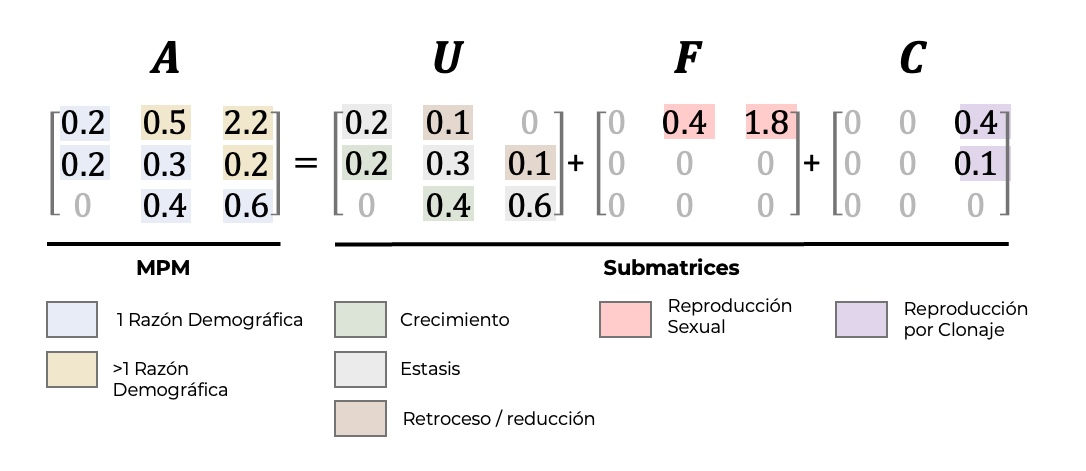
\includegraphics[keepaspectratio,alt={FIGURA 4: La descomposición de un MPP en sus submatrices permite aislar tasas vitales que de otro modo estarían enmascaradas. La matriz A representa la MPP. Dado que las transiciones individuales pueden representarse por múltiples tasas demográficas (por ejemplo, regresión, reproducción sexual y clonalidad), reproducción), descomponer A en sus submatrices U, F y C permite realizar inferencias demográficas específicas sobre qué transiciones demográficas están impulsando la dinámica de la población.}]{images/Matrices_A_U_F_C.jpg}}

4.3 \textbar{} Archivando los datos en COMPADRE y COMADRE

Proponemos que las bases de datos de la matriz de COMPADRE y COMADRE
proporcionen la forma más adecuada de archivar y acceder a MPP's.
Mientras reconocemos que hay otros repositorios de bases de datos
ecológicas (por ejemplo, Dryad: \url{https://datadryad.org/}; figshare:
\url{https://figshare.com}; Zenodo: \url{https://zenodo.org}), la base
de datos de COMPADRE COMADRE de acceso abierto
(\url{https://compadre-db.org/Contribute}) proporciona una plataforma de
archivo de datos dedicada, específicamente para MPP's, que permite
contribuciones directas de los investigadores y la digitalización de MPP
publicados por nuestros equipos de validación de datos. La integración
de un portal usando una pagina web para la entrada de datos proporciona
un proceso de curación de datos estructurado (es decir, desde la
detección, la estandarización, hasta la validación) que pueden acomodar
MPP de diferentes dimensiones y diversas historias de vida. Al ingresar,
los MPP se complementan con variables biogeográficas relevantes y
detalles sobre la metodología del censo en COMPADRE y COMADRE. Detalles
de la publicación original, incluyendo doi y citas funcionales (ver
\url{https://compadre-db.org/Education/article/obtaining-references}
donde se almacenan junto con cada MPP para garantizar que su
contribución a cualquier publicación futura es reconocida. Todos los
datos están archivados a largo plazo a través de Oxford Open Access y
con apoyo de la Biblioteca Bodleian.

Otras mejoras recientes integradas a COMPADRE y COMADRE ayudarán aún más
a la comunidad científica. Anteriormente, las bases de datos solo eran
accesibles a través de la descarga de un archivo R-Object que contenía
todas las matrices en esa versión de la base de datos. La base de datos
es ahora accesible a través de un sitio web
(\url{https://compadre-db.org/QueryDatabase}) que permite a los usuarios
encontrar y descargar matrices individuales. También nos esforzamos por
empoderar a los investigadores y educadores con materiales de enseñanza
(\url{https://compadre-db.org/Education}) y la producción de nuevos
paquetes R ({Jones et~al.}, 2022) para facilitar escalabilidad de MPP
investigación. Junto con estos materiales, todos los detalles de la
estructura de la base de datos y el flujo de trabajo son de acceso libre
(\url{https://jonesor.github.io/CompadreGuides/user-guide.html}). Estas
mejoras en las bases de datos y su estructura de interfaz han sido
directamente dirigidas a equipar a los demógrafos con más herramientas
para realizar investigaciones y capacitar a los estudiantes en MPP's
junto con las mejoras en transparencia de la base de datos para
garantizar buenas prácticas en la investigación.

5 \textbar{} Un protocolo estandarizado para reportar MPP's

Aquí presentamos una lista de verificación propuesta sobre cómo reportar
un MPP en publicaciones (Recuadro 1). Recomendamos utilizar la lista de
verificación cuando diseñar la recopilación de datos, así como al
redactar el MPP para publicación. Recomendamos utilizar esta plantilla
como apoyo de la información necesaria para los MPP ya que permite una
comunicación clara de la construcción de los modelos además de la
facilidad para integrar publicaciones MPP a las bases de datos COMPADRE
y COMADRE.

6 \textbar{} La teoría no es estática: la no linealidad, dependencia del
medio ambiente y los modelos de múltiple estados.

Los MPP se han convertido en un enfoque predominante en la lista de
herramientas en el estudio de ecología de población en parte debido a su
simplicidad de construcción y análisis. Pero la teoría subyacente basada
en matrices para estudiar demografía no se detiene y en los últimos 20
años ha aumentado espectacularmente. Estos nuevos métodos producen
modelos cuya estructura no se ajusta en los marcos para la presentación
de informes que parecían tan completos en el pasado. Estos avances
recientes en la teoría y los métodos de MPP permiten investigadores
vincular la dinámica demográfica y el efecto del medio ambiente sobre la
demografía y múltiples rasgos individuales (por ejemplo, sexo y edad)
(Childs, Sheldon \& Rees, 2016); edad y parentesco (Caswell, 2019a,
2020) en lugar de un solo rasgo de la especie. Estos avances también
ofrecen beneficios para el estudio de respuestas de la población al
clima extremo (Jenouvrier et~al., 2022), en adición de investigaciones
demográfica más matizadas de aspectos comparativos y evolutivos (Childs,
Sheldon \& Rees, 2016). En esta sección repasamos algunas áreas
interesantes de demografía estructurada que pueden abrir nuevas
preguntas de investigación para el demógrafo y enumerar algunos de los
desafíos que plantean para la comunicación y la presentación de
informes.

6.1 \textbar{} Modelos no lineales

Los MPP no lineales son aquellos en los que las entradas de la matriz de
proyección dependen del estado de la población (números y estructura) y
pueden ser influenciados por la frecuencia o la densidad
denso-dependiente. Los modelos que son influenciados por la densidad de
frecuencia no lineal dependen sólo de la relativa abundancia de etapas;
ellos ocurren en los modelos de dos sexos en los que el apareamiento
depende de la relación abundancia de machos y hembras, y en modelos
genéticos de poblaciones donde la dinámica depende de la abundancia
relativa de genotipos (Vries \& Caswell, 2019). Los modelos
denso-dependientes dependen de la abundancia y estructura de la
población; ejemplos recientes incluyen a (Pardini et~al., 2009) y (Shyu
et~al., 2013) para análisis de estrategias de control de la mostaza con
ajo \emph{Alliaria petiolata} y de (Vries \& Caswell, 2019) para
estudios de laboratorio de resistencia a pesticidas en \emph{Tribolium}.

Los análisis de MPP no lineales se centran en los resultados
demográficos diferentes a los de los modelos lineales; equilibrios,
atractores, bifurcaciones, oscilaciones y estabilidad Cushing (2003).
Sin embargo, ¿qué hace que estos modelos sean problemáticos para la
situación actual? El estatus de COMPADRE y COMADRE es que la unidad del
modelo no es una matriz, sino más bien una función matricial, en la que
las entradas de la matriz de proyección son funciones del estado de la
población. Los análisis de sensibilidad están disponibles para estudiar
prácticamente cualquier grupo demográfico resultado en respuesta a
cualquier parámetro (Caswell, 2019b), pero informar las funciones que
definen el MPP no lo es en absoluto estandarizado.

6.2 \textbar{} Dependencia del Ambiente

Un problema similar surge en entornos dependientes del medio ambiente.
En algunos modelos, algunas o todas las tasas demográficas son funciones
de algunos aspectos del medio ambiente; por ejemplo, los osos polares
como funciones de los parámetros estadísticos del hielo marino del
Ártico (Regehr et~al., 2010), los sifaka de Madagascar como funciones de
lluvia (Lawler et~al., 2009), el pingüino emperador en función de los
patrones estacionales del hielo marino en la Antártida (Jenouvrier
et~al., 2012) y la ballena franca del Atlántico norte en función del
tiempo y de las tendencias en el tiempo (Fujiwara \& Caswell, 2001). Al
igual que con los MPP no lineales, el modelo no es una matriz, sino una
función que se mapea desde las variable(s) ambientales a las entradas de
la matriz. Los protocolos para informar dichas funciones aún no están
disponibles pero es importante desarrollarlas.

6.3 \textbar{} Modelos de múltiples estados

Un área emergente en la investigación demográfica es la construcción y
análisis de MPP multiestatales, en los que se clasifican los individuos
por más de una variable de estado. Esto incluye edad y etapa. (Caswell
\& Salguero-Gómez, 2013), escenario y localización espacial (Hunter \&
Caswell, 2005), estadio y genotipo (Vries \& Caswell, 2019), estadio y
estado de infección (Klepac \& Caswell, 2011), edad y heterogeneidad no
medida (Hartemink, Missov \& Caswell, 2017) y etapas específicas de
incidencia de enfermedades (Caswell \& Daalen, 2021). Una presentación
detallada de los métodos se encuentra en (Caswell et~al., 2018) y la
extensión a más de dos ejes estatales (los llamados matrices de
hiperestado) se proporciona en (Roth \& Caswell, 2016). La incorporación
de estados adicionales permite a los investigadores separar varias
fuentes de información individual de heterogeneidad, la varianza en la
historia de vida de los individuos del mismo modelo poblacional y sus
resultados, en adición de plantear comparaciones más profundas y
preguntas evolutivas. Por ejemplo, la edad materna tiene un fuerte
impacto en las tasas vitales en rotíferos monogonones (Bock et~al.,
2019). Aplicando métodos de permutación-vec (Caswell, 2012) para
construir MPP multi-estatales han permitido a los investigadores
cuantificar el nivel de población impactos del efecto observado de la
edad materna e investigar los procesos evolutivos que pueden conducir a
este tipo de senescencia en rotíferos (Hernández et~al., 2020). MPP
multidimensionales y los métodos de la cadena de Markov han sido
particularmente importantes en el estudio de la ``suerte'' en las
historias de vida, que explora por qué algunos individuos viven mucho
tiempo y prosperan, mientras que otros no (Snyder \& Ellner, 2022). En
estudios de ``suerte'', la variación entre individuos en la historia de
vida se divide en contribuciones de la variación entre grupos y dentro
del grupo por ejemplo, (Daalen \& Caswell, 2017; Snyder \& Ellner,
2018). Ejemplos de fuentes de heterogeneidad individual incluyen edad
materna (Daalen et~al., 2022), año de nacimiento ambiente (Snyder \&
Ellner, 2022) y variación genética (Steiner, Tuljapurkar \& Roach,
2021). El efecto de la variación dentro se llama estocasticidad
individual o ``suerte'' y surge del hecho de que las tasas vitales son
procesos probabilísticos.

Estos modelos plantean un desafío para la presentación de informes
porque el MPP no consta de una única matriz, sino de cuatro conjuntos de
matrices. Considerar un modelo clasificado como edad × etapa. Esos
modelos están compuestos por un conjunto de matrices dando transiciones
entre etapas para cada clase de edad, un conjunto de matrices D
asignando transiciones de edad para cada etapa y un conjunto de matrices
F que asignan transiciones de edad específicas para cada etapa de
fecundidad, y un conjunto de matrices H que asignan crías recién nacidas
a las edades apropiadas. Estos están ensamblados en matrices de
transición y fertilidad estructuradas en bloques a partir de las cuales
todos los resultados demográficos habituales se pueden calcular y
relacionar con tanto la edad como la etapa (por ejemplo, ver Caswell \&
Salguero-Gómez, 2013 para un análisis de gradientes de selección tanto
para edad como para tamaño).

7 \textbar{} Discusión

La investigación demográfica ha avanzado mucho desde la introducción de
los estudios demográficos a base de edad (Leslie, 1945) y modelos
matriciales basado en etapas (Lefkovitch, 1965). Los avances en este
campo se han visto impulsados en parte mediante una comunicación clara
de los métodos y el código asociado. Deseamos continuar expandiendo el
uso de esas herramientas con la comunicación de MPP.

A medida que la profundidad y amplitud de la literatura continúa
expandiéndose, estamos empezando a construir una imagen integral de la
demografía y explorar el espectro de la vida biológica (Adler et~al.,
2014; Salguero-Gomez et~al., 2017; Healy et~al., 2019). A través de la
base de datos de COMPADRE y COMADRE, hemos llegado a apreciar la
utilidad y oportunidades de una forma estandarizada de compilar MPP. De
hecho, una parte importante del tiempo (\textgreater50\%) que dedicamos
a curar estas bases de datos en realidad no se trata de digitalización,
verificación de errores, y complementar datos, sino en contactar a los
autores para obtener aclaraciones y solicitud de datos y metadatos
faltantes. A través de este arduo proceso, hemos identificado valiosas
información en MPP que no estaba en las publicaciones originales. Si
bien los datos faltantes se destacan aquí como particularmente
importante y refleja principalmente los intereses y perspectivas de
demógrafos comparativos, incluidos los datos descritos en el métodos
estandarizado que beneficiaría a la demografía en su conjunto.

Este artículo pretende actuar como una referencia útil para autores,
editores, revisores, gestores/conservacionistas y demógrafos
comparativos. Además, esperamos que este manuscrito promueva una
discusión constructiva sobre el propósito, la construcción y la
presentación de información demográfica a base de etapas. El cuadro 1
contiene un ejemplo completo de la información clave que creemos que
debería incorporarse a la publicación de cualquier MPP. Al adoptarse los
métodos que se sugieren aquí, habrá claros beneficios para el
crecimiento de las bases de datos demográficas COMPADRE y COMADRE; sin
embargo, creemos que estos beneficios se extienden más allá de COMPADRE
y usuarios de COMADRE hacia todo el campo de la ecología de poblaciones
y campos que utilizan MPP para su propia beneficio (por ejemplo,
conservación biología y monitoreo de la biodiversidad). Un mayor nivel
de detalle y transparencia al describir cómo y por qué se produce un MPP
dará como resultado una mayor precisión, accesibilidad, reproducibilidad
y citabilidad; eso tiene claros beneficios para el campo en su conjunto
y para los investigadores. Además, una mayor coherencia y transparencia
facilita la revisión por pares y, de hecho, estas directrices pueden
ofrecer una herramienta que puede ser citada por editores asociados y
revisores por pares y puede ser recomendado como guía para los pasos
sugeridos aquí. Además, la adopción de los pasos sugeridos aquí puede
aumentar confianza en los resultados presentados y facilitar el
aprendizaje/adopción de MPP por investigadores que inician su carrera.

Finalmente, cerramos con una precaución. Hemos utilizado el término
``preciso'' en puntos a lo largo de este documento, aplicados a los MPP,
pero debemos reconocer que no existe un modelo exacto, ya sea un MPP o
cualquier otro tipo. Un modelo es una serie de selección de parámetros,
selección de aspectos o variables que se incluyen y otros que no se
incluye. La selección de modelos como técnicas de selección como AIC
(Akaike Information Criterion; (Anderson \& Burnham, 2002) hacen estas
opciones explícitas y miden su apoyo en términos de probabilidad. Pero
incluso sin utilizar el método estadístico explícito, el mensaje es
claro. Las opciones de ``i''-estado/variables, de intervalos de
proyección, de tipos de variación temporal, de dependencia funcional de
un conjunto elegido de factores ambientales, etc., todos ellos son
inexactos. La cuestión no es buscar la precisión: es ser claro al
comunicar las decisiones que tomó al construir el modelo, los análisis
que usted eligió aplicar y la interpretación de los resultados. Un
modelo `preciso' de un sistema ecológico, experimental u observacional
sería tan complicado como un sistema real. Eso no termina bien (Borges,
1999).

Supporting Information

Additional supporting information can be found online in the Supporting
Information section at the end of this article. Data S1: A survey on
matrix communication.

\bookmarksetup{startatroot}

\chapter{Impactos de datos sin sentido
biológico}\label{ImpactosSinSentido}

Por: Raymond L. Tremblay

\subsubsection{Librerías de R requeridas para el siguiente
módulo}\label{libreruxedas-de-r-requeridas-para-el-siguiente-muxf3dulo-16}

\begin{Shaded}
\begin{Highlighting}[]
\CommentTok{\#devtools::install\_github("rich{-}iannone/DiagrammeR") \# Instalar directamente de github para tener la versión más reciente}
\ControlFlowTok{if}\NormalTok{ (}\SpecialCharTok{!}\FunctionTok{require}\NormalTok{(}\StringTok{"pacman"}\NormalTok{)) \{}
  \FunctionTok{install.packages}\NormalTok{(}\StringTok{"pacman"}\NormalTok{)}
\NormalTok{\}}
\NormalTok{pacman}\SpecialCharTok{::}\FunctionTok{p\_load}\NormalTok{(}
  \StringTok{"DiagrammeR"}\NormalTok{,}
  \StringTok{"Rage"}\NormalTok{,}
  \StringTok{"popdemo"}\NormalTok{,}
  \StringTok{"popbio"}\NormalTok{,}
  \StringTok{"interpretCI"}\NormalTok{,}
  \StringTok{"MCMCpack"}\NormalTok{,}
  \StringTok{"ggplot2"}\NormalTok{,}
  \StringTok{"plyr"}\NormalTok{,}
  \StringTok{"reshape2"}
\NormalTok{)}

\FunctionTok{library}\NormalTok{(DiagrammeR)}
\FunctionTok{library}\NormalTok{(Rage)}
\FunctionTok{library}\NormalTok{(popdemo)}
\FunctionTok{library}\NormalTok{(popbio)}
\FunctionTok{library}\NormalTok{(tidyverse)}
\FunctionTok{library}\NormalTok{(flextable)}
\FunctionTok{library}\NormalTok{(interpretCI)}
\FunctionTok{library}\NormalTok{(MCMCpack)}
\FunctionTok{library}\NormalTok{(plyr)}
\FunctionTok{library}\NormalTok{(reshape2)}
\end{Highlighting}
\end{Shaded}

\begin{Shaded}
\begin{Highlighting}[]
\NormalTok{rlt\_theme }\OtherTok{\textless{}{-}} \FunctionTok{theme}\NormalTok{(}
  \AttributeTok{axis.title.y =} \FunctionTok{element\_text}\NormalTok{(}\AttributeTok{colour =} \StringTok{"grey20"}\NormalTok{, }\AttributeTok{size =} \DecValTok{10}\NormalTok{, }\AttributeTok{face =} \StringTok{"bold"}\NormalTok{),}
  \AttributeTok{axis.text.x =} \FunctionTok{element\_text}\NormalTok{(}\AttributeTok{colour =} \StringTok{"grey20"}\NormalTok{, }\AttributeTok{size =} \DecValTok{10}\NormalTok{, }\AttributeTok{face =} \StringTok{"bold"}\NormalTok{),}
  \AttributeTok{axis.text.y =} \FunctionTok{element\_text}\NormalTok{(}\AttributeTok{colour =} \StringTok{"grey20"}\NormalTok{, }\AttributeTok{size =} \DecValTok{15}\NormalTok{, }\AttributeTok{face =} \StringTok{"bold"}\NormalTok{),}
  \AttributeTok{axis.title.x =} \FunctionTok{element\_text}\NormalTok{(}\AttributeTok{colour =} \StringTok{"grey20"}\NormalTok{, }\AttributeTok{size =} \DecValTok{15}\NormalTok{, }\AttributeTok{face =} \StringTok{"bold"}\NormalTok{)}
\NormalTok{) }\SpecialCharTok{+}
  \FunctionTok{theme}\NormalTok{(}
    \CommentTok{\# Remover los bordes}
    \AttributeTok{panel.border =} \FunctionTok{element\_blank}\NormalTok{(),}
    \CommentTok{\# Remover las líneas}
    \AttributeTok{panel.grid.major =} \FunctionTok{element\_blank}\NormalTok{(),}
    \AttributeTok{panel.grid.minor =} \FunctionTok{element\_blank}\NormalTok{(),}
    \CommentTok{\# Remover el fondo del panel}
    \AttributeTok{panel.background =} \FunctionTok{element\_blank}\NormalTok{(),}
    \CommentTok{\# añadir lineas más gruesas}
    \AttributeTok{axis.line.x =} \FunctionTok{element\_line}\NormalTok{(}\AttributeTok{colour =} \StringTok{"black"}\NormalTok{, }\AttributeTok{linewidth =} \DecValTok{1}\NormalTok{),}
    \AttributeTok{axis.line.y =} \FunctionTok{element\_line}\NormalTok{(}\AttributeTok{colour =} \StringTok{"black"}\NormalTok{, }\AttributeTok{linewidth =} \DecValTok{1}\NormalTok{)}
\NormalTok{  )}

\NormalTok{diverging}\OtherTok{=} \FunctionTok{c}\NormalTok{(}\StringTok{"\#009392"}\NormalTok{,}\StringTok{"\#CF597E"}\NormalTok{,}\StringTok{"\#E9E29C"}\NormalTok{, }\StringTok{"\#39B185"}\NormalTok{,}\StringTok{"\#EEB479"}\NormalTok{ , }\StringTok{"\#9CCB86"}\NormalTok{ )}

\CommentTok{\# {-}{-}{-} 2. Combinarlos en un objeto de tipo lista {-}{-}{-}}
\CommentTok{\# Esta lista se puede añadir al gráfico con un solo \textquotesingle{}+\textquotesingle{}}
\NormalTok{rlt\_style\_fill }\OtherTok{\textless{}{-}} \ControlFlowTok{function}\NormalTok{() \{}
  \FunctionTok{list}\NormalTok{(}
\NormalTok{    rlt\_theme,}
    \FunctionTok{scale\_fill\_manual}\NormalTok{(}\AttributeTok{values =}\NormalTok{ diverging)}
\NormalTok{  )}
\NormalTok{\}}

\NormalTok{rlt\_style\_colour }\OtherTok{\textless{}{-}} \ControlFlowTok{function}\NormalTok{() \{}
  \FunctionTok{list}\NormalTok{(}
\NormalTok{    rlt\_theme,}
    \FunctionTok{scale\_colour\_manual}\NormalTok{(}\AttributeTok{values =}\NormalTok{ diverging)}
\NormalTok{  )}
\NormalTok{\}}
\end{Highlighting}
\end{Shaded}

El valor principal de los estudios científicos radica en el supuesto de
que los datos obtenidos representan una versión suficientemente cercana
de la realidad biológica de campo, de modo que puedan utilizarse para
inferir sobre la ecología y conservación de las especies de interés.
Este supuesto de que los datos representan realmente a la realidad es un
mito, ya que solamente son una muestra, que esperamos que se acerque lo
suficiente para tener confianza en los resultados. En ningún estudio
ecológico se podrán obtener \textbf{TODOS} los datos para evaluar todas
las relaciones bióticas y abióticas que mantiene un organismo y sus
interacciones. Dicho modelo sería demasiado complejo e irreal dentro del
concepto de lo que se puede lograr en un trabajo científico. Es por ello
que, el objetivo de estos trabajos es tener una apreciación de los
parámetros más importantes para definir patrones e interacciones
suficientemente cercanas a la realidad para ser útiles. Por
consiguiente, la base de estos estudios está sostenida en las unidades
de muestreo y en la recolección de datos. Si los datos no representan la
realidad, las interpretaciones de los análisis pueden ser erróneas. La
matemática, con sus ecuaciones y sus modelos, no hará que la biología se
aproxime más a la realidad, si desde el principio los datos y el método
de recolección de datos son erróneos.

Es por ello que en esta sección evaluaremos diferentes aspectos de los
análisis matriciales poblacionales de proyección (MPP) y diferentes
aspectos de la recolección de datos que pudiesen ser problemáticos
cuando uno considera la biología de una especie. La lista de
\emph{Impactos} no pretende incluir todos los posibles efectos de datos
sin sentido; sino más bien, brindar algunos ejemplos de lo que pasa
cuando uno no considera estos problemas y cómo pueden distorsionar las
interpretaciones. Por lo tanto, se les extiende una advertencia a todos
los biólogos de poblaciones, para que estén conscientes de estos temas y
siempre evalúen críticamente sus datos desde la forma de recolección, su
análisis e interpretaciones de sus resultados y aceptar que son
solamente un modelo (una caricatura) de muchos posibles modelos.

\begin{center}\rule{0.5\linewidth}{0.5pt}\end{center}

\section{Cuatro familias de errores}\label{cuatro-familias-de-errores}

Los problemas que pueden invalidar un análisis matricial poblacional
caen en cuatro grandes grupos. Conocerlos por separado ayuda a saber
\textbf{dónde mirar} cuando algo no cuadra:

\begin{enumerate}
\def\labelenumi{\arabic{enumi}.}
\item
  \textbf{Errores en la recolección de datos.} Tamaños de muestra
  pequeños, eventos raros que nunca se observaron en el periodo de
  estudio, etapas crípticas (semillas, latencia, juveniles ocultos) que
  no se detectan. Síntoma típico: probabilidades de transición
  exactamente iguales a 0 o a 1.
\item
  \textbf{Errores en la construcción de la matriz.} Supervivencia
  perfecta (columnas que suman 1 sin reproducción), columnas que suman
  \emph{más} de 1 por redondeo excesivo, transiciones biológicamente
  posibles que faltan en la matriz (matrices reducibles).
\item
  \textbf{Errores en la fecundidad.} Usar el número crudo de
  semillas/huevos en vez de los individuos que efectivamente reclutan al
  primer estadio del modelo, omitir el banco de semillas, no especificar
  si el censo es pre- o post-reproductivo (ver el
  \hyperref[protocolo]{protocolo estandarizado del capítulo 121}).
\item
  \textbf{Errores en la inferencia estadística.} Calcular intervalos de
  confianza con la distribución normal sobre proporciones acotadas en
  {[}0, 1{]} ---que produce límites negativos o mayores que 1---, no
  comunicar la incertidumbre de los parámetros.
\end{enumerate}

Para cada error mostraremos tres cosas: \textbf{cómo se ve} en el código
y la matriz, \textbf{cómo detectarlo en R}, y \textbf{cómo evitarlo o
corregirlo}. Así el capítulo sirve tanto como guía de lectura crítica de
la literatura como lista de verificación al construir su propio MPP.

\begin{tcolorbox}[enhanced jigsaw, arc=.35mm, bottomrule=.15mm, bottomtitle=1mm, breakable, colback=white, colbacktitle=quarto-callout-tip-color!10!white, colframe=quarto-callout-tip-color-frame, coltitle=black, left=2mm, leftrule=.75mm, opacityback=0, opacitybacktitle=0.6, rightrule=.15mm, title=\textcolor{quarto-callout-tip-color}{\faLightbulb}\hspace{0.5em}{¿Cuándo regresar a este capítulo?}, titlerule=0mm, toprule=.15mm, toptitle=1mm]

Este capítulo está diseñado para consultarse en dos momentos distintos:
\textbf{antes} de comenzar el muestreo, para anticipar qué decisiones de
diseño afectarán la matriz, y \textbf{después} de tener una matriz
preliminar, para diagnosticarla antes de pasar a inferencias o
publicación. Léalo con su matriz al lado.

\end{tcolorbox}

\begin{center}\rule{0.5\linewidth}{0.5pt}\end{center}

\section{Tamaños de muestra pequeños o eventos
raros}\label{tamauxf1os-de-muestra-pequeuxf1os-o-eventos-raros}

Sin duda, el tema principal para el uso de MPP ha sido evaluar la
proyección de población de especies raras o en peligro de extinción
(Caswell, 1989b; {Gascoigne et~al.}, 2023). En consecuencia, las
especies raras o en peligro de extinción son naturalmente pequeñas y el
tamaño de la muestra del estudio o de algunas de las etapas/edades del
ciclo de vida son frecuentemente pequeños. Estos tamaños de muestra
reducidos suelen provocar estimaciones sesgadas de los parámetros y, a
menudo, resultados sin sentido biológico. Algunos de los problemas
incluyen no haber observado eventos raros (transiciones poco comunes),
como la muerte de un adulto o la germinación de una semilla. En estos
casos, la probabilidad de supervivencia o transición pudiese ser de
cero, lo que pudiese resultar en una matriz reducible o no irreducible.

\begin{center}\rule{0.5\linewidth}{0.5pt}\end{center}

\subsection{Supervivencia perfecta}\label{supervivencia-perfecta}

Muestreos en donde no se observa mortalidad, que equivaldrían a una
supervivencia perfecta, son problemáticos. Esto se pudiese observar
generalmente en especies longevas, en donde la mortalidad de los
individuos, en especial de los individuos adultos es rara, pero la
probabilidad existe. Considere una especie donde se recopilan datos de
la especie \textbf{Sp1} y se crea una matriz de transición
\textbf{Sp1matU} y una matriz de fertilidad \textbf{Sp1matF}. Note que
ninguno de los individuos adultos muestreados murió, por lo que el valor
de la permanencia es de 1 (supervivencia perfecta). En consecuencia, el
tamaño de la población nunca disminuye. Sin embargo, esto es
completamente irreal. Así, bajo todos los modelos biológicamente
realistas, esperaríamos que el tamaño de la población comience a
disminuir si una población no tiene reproducción. Sin embargo, en
nuestro ejemplo, a pesar de que la fecundidad es cero, nuestra población
se mantiene ya que los individuos adultos presentan una supervivencia
perfecta, lo cual es biológicamente imposible.

\begin{Shaded}
\begin{Highlighting}[]
\NormalTok{Sp1matU }\OtherTok{\textless{}{-}} \FunctionTok{rbind}\NormalTok{(}
  \FunctionTok{c}\NormalTok{(}\FloatTok{0.0}\NormalTok{, }\FloatTok{0.0}\NormalTok{, }\FloatTok{0.0}\NormalTok{),}
  \FunctionTok{c}\NormalTok{(}\FloatTok{0.5}\NormalTok{, }\FloatTok{0.3}\NormalTok{, }\FloatTok{0.0}\NormalTok{),}
  \FunctionTok{c}\NormalTok{(}\FloatTok{0.0}\NormalTok{, }\FloatTok{0.4}\NormalTok{, }\FloatTok{1.0}\NormalTok{)}
\NormalTok{) }\CommentTok{\# transition matrix}

\NormalTok{Sp1matF }\OtherTok{\textless{}{-}} \FunctionTok{rbind}\NormalTok{(}
  \FunctionTok{c}\NormalTok{(}\FloatTok{0.0}\NormalTok{, }\FloatTok{0.0}\NormalTok{, }\FloatTok{0.0}\NormalTok{),}
  \FunctionTok{c}\NormalTok{(}\FloatTok{0.0}\NormalTok{, }\FloatTok{0.0}\NormalTok{, }\FloatTok{0.0}\NormalTok{),}
  \FunctionTok{c}\NormalTok{(}\FloatTok{0.0}\NormalTok{, }\FloatTok{0.0}\NormalTok{, }\FloatTok{0.0}\NormalTok{)}
\NormalTok{) }\CommentTok{\# fertility matrix}

\NormalTok{Sp1matA }\OtherTok{=}\NormalTok{ Sp1matU }\SpecialCharTok{+}\NormalTok{ Sp1matF }\CommentTok{\# TF matrix}

\FunctionTok{lambda}\NormalTok{(Sp1matA) }\CommentTok{\# lambda es 1, lo que indica que la población no cambia}
\end{Highlighting}
\end{Shaded}

\begin{verbatim}
[1] 1
\end{verbatim}

\begin{Shaded}
\begin{Highlighting}[]
\NormalTok{stages }\OtherTok{\textless{}{-}} \FunctionTok{c}\NormalTok{(}\StringTok{"plantula"}\NormalTok{, }\StringTok{"juvenil"}\NormalTok{, }\StringTok{"adulto"}\NormalTok{)}

\FunctionTok{plot\_life\_cycle}\NormalTok{(Sp1matA, }\AttributeTok{stages =}\NormalTok{ stages, }\AttributeTok{fontsize =} \DecValTok{0}\NormalTok{)}
\end{Highlighting}
\end{Shaded}

\pandocbounded{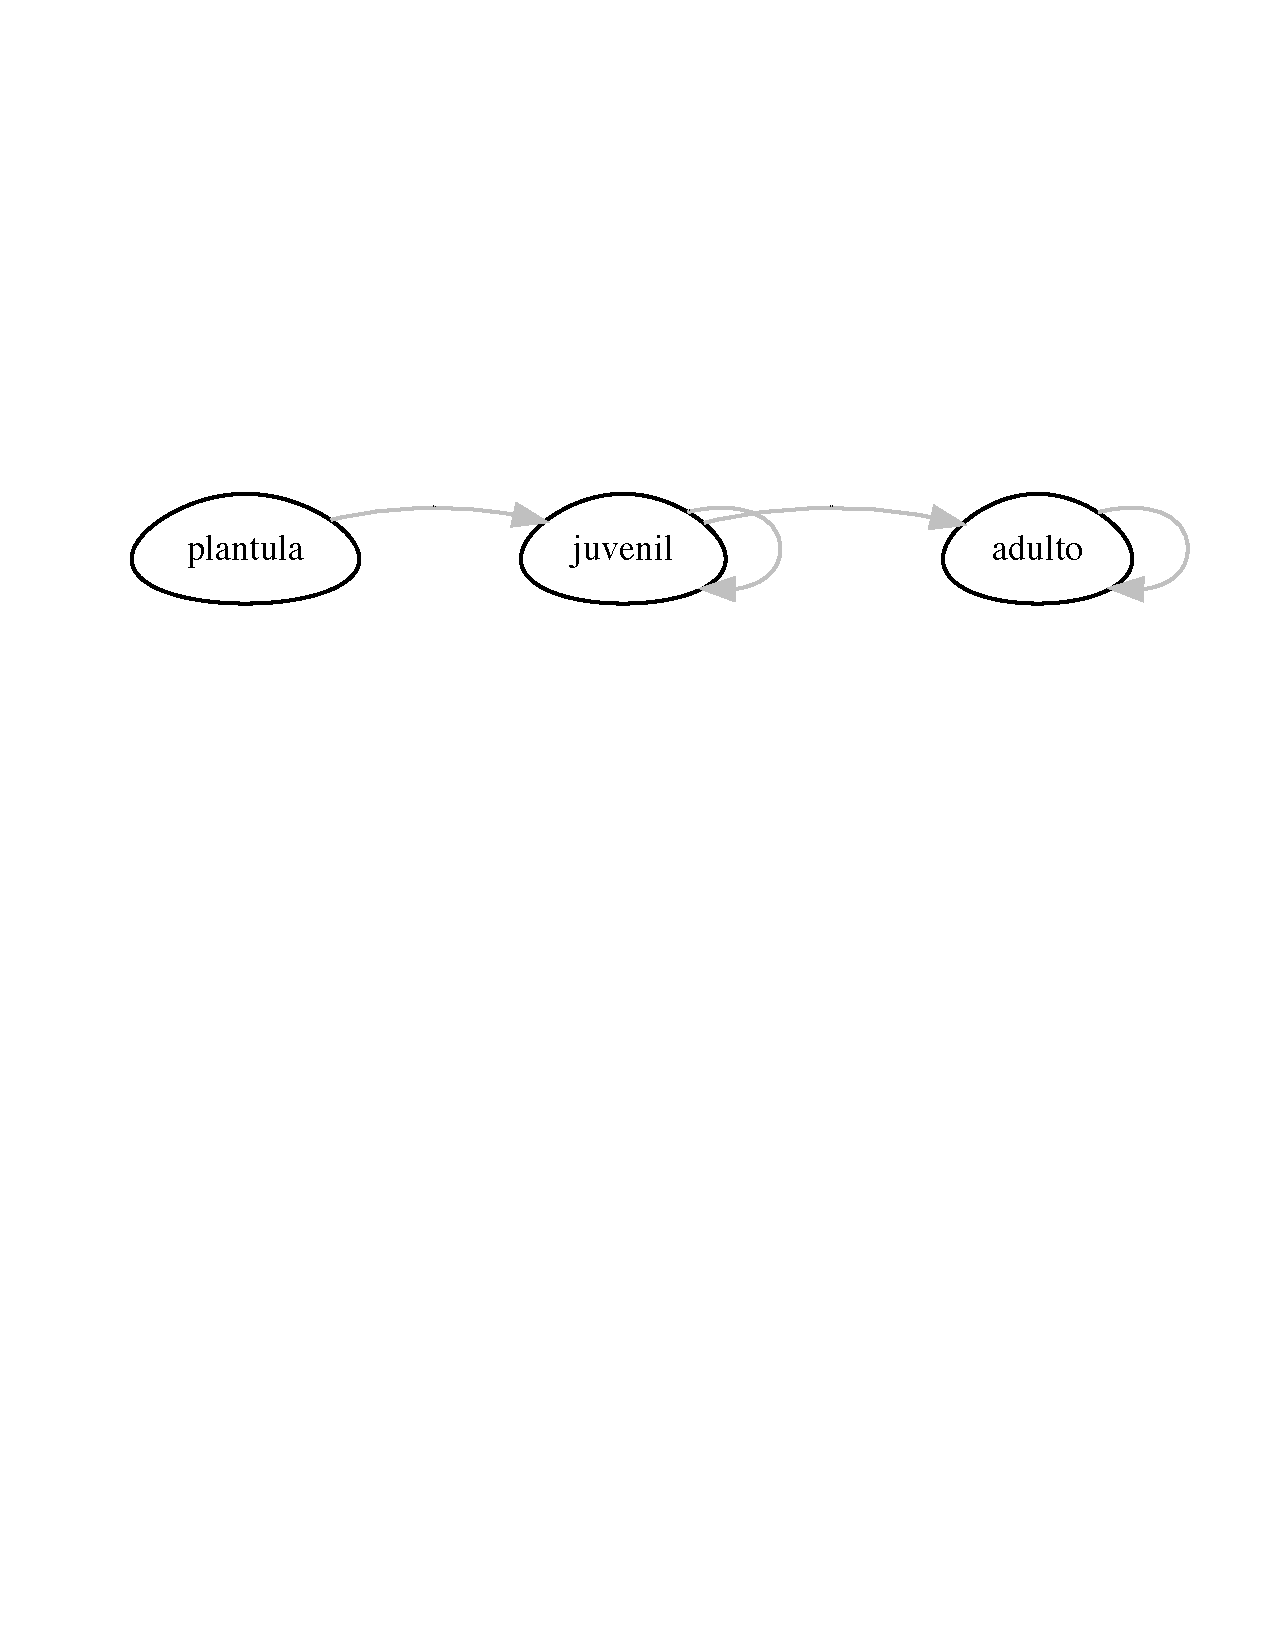
\includegraphics[keepaspectratio]{122-Impacto_de_Datos_sin_Sentido_files/figure-pdf/sin_sentido_2-1.pdf}}

Si analizamos \textbf{Sp1matU}, asumimos que ninguno de los individuos
muestreados en etapa adulta muere, en ningún momento!!! Claramente esto
no es realista. Para cualquier especie, la probabilidad de muerte en
cualquier etapa nunca es cero (aunque podría ser muy pequeña) y, por lo
tanto, nuestra matriz no tiene sentido biológico. Considere una especie
de árbol, como los árboles de \emph{Sequoia}, en donde es muy probable
que la supervivencia de los árboles grandes sea muy alta entre un año y
otro y por lo tanto la \textbf{supervivencia observada} sea del 100\%,
pero, este 100\% no es realista a largo plazo. Hay que diferenciar entre
lo que se observa en un periodo de muestreo y las probabilidades a largo
plazo. Es posible que en el sitio de estudio NO se observó mortalidad de
los árboles grandes entre los dos periodos de muestreo, lo que
resultaría en una mortalidad de cero, sin embargo, este valor no es real
a largo plazo. Ese estimado de campo puede ser un resultado de un tamaño
de muestra insuficiente o de eventos raros (aun con tamaños de muestra
grandes).

En el siguiente \emph{script} mostramos que la población no cambia
después de 7-8 periodos/años y se mantiene cercana a uno (usamos la
matriz de transición sin fecundidad). Si no hay reclutas (matriz de
fertilidad), el tamaño de la población debería reducirse con el tiempo.
Todos los modelos de transiciones que no incluyan a la matriz de
fertilidad (solamente la matU), deberían resultar en reducción de tamaño
poblacional en el tiempo, debido a la no incorporación de nuevos
individuos (fecundidad), de la pérdida de individuos muestreados
(mortalidad).

\begin{Shaded}
\begin{Highlighting}[]
\NormalTok{n }\OtherTok{=} \FunctionTok{c}\NormalTok{(}\DecValTok{50}\NormalTok{, }\DecValTok{50}\NormalTok{, }\DecValTok{50}\NormalTok{)}

\FunctionTok{truelambda}\NormalTok{(Sp1matU) }\CommentTok{\# despues de unos periodos de tiempo vemos que el crecimiento poblacional es 1}
\end{Highlighting}
\end{Shaded}

\begin{verbatim}
          [,1] [,2]
[1,] 0.9999999    1
[2,] 0.9999999    1
[3,] 0.9999999    1
\end{verbatim}

\begin{Shaded}
\begin{Highlighting}[]
\FunctionTok{pop.projection}\NormalTok{(Sp1matU, }\AttributeTok{n =}\NormalTok{ n)}\SpecialCharTok{$}\NormalTok{pop.changes }\CommentTok{\# lista del cambio poblacional en 19 años}
\end{Highlighting}
\end{Shaded}

\begin{verbatim}
 [1] 0.7333333 0.8909091 0.9632653 0.9885593 0.9965281 0.9989548 0.9996861
 [8] 0.9999058 0.9999717 0.9999915 0.9999975 0.9999992 0.9999998 0.9999999
[15] 1.0000000 1.0000000 1.0000000 1.0000000 1.0000000
\end{verbatim}

\begin{tcolorbox}[enhanced jigsaw, arc=.35mm, bottomrule=.15mm, bottomtitle=1mm, breakable, colback=white, colbacktitle=quarto-callout-warning-color!10!white, colframe=quarto-callout-warning-color-frame, coltitle=black, left=2mm, leftrule=.75mm, opacityback=0, opacitybacktitle=0.6, rightrule=.15mm, title=\textcolor{quarto-callout-warning-color}{\faExclamationTriangle}\hspace{0.5em}{Cómo detectar y resolver --- supervivencia perfecta}, titlerule=0mm, toprule=.15mm, toptitle=1mm]

\textbf{Detección en R:}

\begin{Shaded}
\begin{Highlighting}[]
\FunctionTok{any}\NormalTok{(}\FunctionTok{diag}\NormalTok{(matU) }\SpecialCharTok{\textgreater{}=} \DecValTok{1}\NormalTok{)              }\CommentTok{\# ¿hay estasis con probabilidad 1?}
\FunctionTok{any}\NormalTok{(}\FunctionTok{colSums}\NormalTok{(matU) }\SpecialCharTok{\textgreater{}=} \DecValTok{1} \SpecialCharTok{\&} \FunctionTok{colSums}\NormalTok{(matF) }\SpecialCharTok{==} \DecValTok{0}\NormalTok{)  }\CommentTok{\# ¿columna que suma 1 sin reproducción?}
\end{Highlighting}
\end{Shaded}

\textbf{Causa típica:} tamaño de muestra insuficiente para observar la
mortalidad rara de los adultos durante el periodo de estudio.

\textbf{Cómo evitarlo o corregirlo:}

\begin{enumerate}
\def\labelenumi{\arabic{enumi}.}
\tightlist
\item
  Reportar el tamaño de muestra de cada etapa y la incertidumbre
  asociada (ver capítulo bayesiano).
\item
  Usar un previo bayesiano informado vía \texttt{raretrans} o una
  distribución de Dirichlet para inferir una mortalidad pequeña pero
  \texttt{\textgreater{}\ 0}.
\item
  Si se decide mantener \texttt{0.995} o similar, justificar el valor
  con literatura sobre la longevidad de la especie y reconocer la
  limitación.
\end{enumerate}

\end{tcolorbox}

\begin{center}\rule{0.5\linewidth}{0.5pt}\end{center}

\subsubsection{Un cambio pequeño en la
mortalidad.}\label{un-cambio-pequeuxf1o-en-la-mortalidad.}

El efecto de aumentar el tamaño de muestra impacta directamente los
posibles valores en la matriz. Considere la siguiente situación. Si
tenemos solamente cinco individuos en la etapa uno, ¿cuáles son los
posibles valores de mortalidad? Esto dependería del número de individuos
que mueran, que pudiera ser ninguno,1, 2,\ldots o todos. Entonces las
probabilidades que pudieran entrar en la matriz dependiendo el número de
individuos muertos serían: 0, 0.2, 0.4, 0.6, 0.8, 1.0. Note que los
valores intermedios no pueden existir en la matriz. Por lo tanto, si uno
tiene un tamaño de muestra pequeño, es probable que los valores en la
matriz no representen la realidad biológica, pero si representan lo
observado en el muestreo de campo.

Si consideramos la matriz del script 3 y observamos el valor de la
permanencia (sobrevivencia) de los individuos adultos podemos deducir
que se muestrearon 1000 individuos y que 995 sobrevivieron. Así con
tamaños muestrales superiores, por ejemplo 1000, además de conferir una
mayor confianza en el parámetro, permite la existencia de valores
intermedios. Tenga en cuenta que en este nuevo modelo de la especie
\emph{SP1}, aunque la tasa de supervivencia es muy cercana a 100\%
(0.995), existe mortalidad y por tanto existiría una disminución de la
población en cada período de tiempo (aunque solo sea en una pequeña
fracción), si los valores de fecundidad fueran de cero. Siempre hay que
considerar si esta tasa de mortalidad es biológicamente real o es un
resultado del tamaño de la muestra.

\begin{Shaded}
\begin{Highlighting}[]
\NormalTok{Sp1matU\_2 }\OtherTok{\textless{}{-}} \FunctionTok{rbind}\NormalTok{(}
  \FunctionTok{c}\NormalTok{(}\FloatTok{0.0}\NormalTok{, }\FloatTok{0.0}\NormalTok{, }\FloatTok{0.0}\NormalTok{),}
  \FunctionTok{c}\NormalTok{(}\FloatTok{0.5}\NormalTok{, }\FloatTok{0.3}\NormalTok{, }\FloatTok{0.0}\NormalTok{),}
  \FunctionTok{c}\NormalTok{(}\FloatTok{0.0}\NormalTok{, }\FloatTok{0.4}\NormalTok{, }\FloatTok{0.995}\NormalTok{)}
\NormalTok{) }\CommentTok{\# transition matrix}

\NormalTok{Sp1matF }\OtherTok{\textless{}{-}} \FunctionTok{rbind}\NormalTok{(}
  \FunctionTok{c}\NormalTok{(}\FloatTok{0.0}\NormalTok{, }\FloatTok{0.0}\NormalTok{, }\FloatTok{1.0}\NormalTok{),}
  \FunctionTok{c}\NormalTok{(}\FloatTok{0.0}\NormalTok{, }\FloatTok{0.0}\NormalTok{, }\FloatTok{0.0}\NormalTok{),}
  \FunctionTok{c}\NormalTok{(}\FloatTok{0.0}\NormalTok{, }\FloatTok{0.0}\NormalTok{, }\FloatTok{0.0}\NormalTok{)}
\NormalTok{) }\CommentTok{\# fertility matrix}

\NormalTok{Sp1matA\_2 }\OtherTok{=}\NormalTok{ Sp1matU\_2 }\SpecialCharTok{+}\NormalTok{ Sp1matF}

\FunctionTok{lambda}\NormalTok{(Sp1matA\_2) }\CommentTok{\# lambda es 0.995, lo que indica que la población disminuye}
\end{Highlighting}
\end{Shaded}

\begin{verbatim}
[1] 1.185514
\end{verbatim}

\begin{Shaded}
\begin{Highlighting}[]
\FunctionTok{pop.projection}\NormalTok{(Sp1matU\_2, }\AttributeTok{n =}\NormalTok{ n)}\SpecialCharTok{$}\NormalTok{pop.changes }\CommentTok{\# lista del cambio poblacional en 19 años}
\end{Highlighting}
\end{Shaded}

\begin{verbatim}
 [1] 0.7316667 0.8874829 0.9586555 0.9836264 0.9915311 0.9939504 0.9946832
 [8] 0.9949045 0.9949712 0.9949913 0.9949974 0.9949992 0.9949998 0.9949999
[15] 0.9950000 0.9950000 0.9950000 0.9950000 0.9950000
\end{verbatim}

\begin{figure}[H]

{\centering \pandocbounded{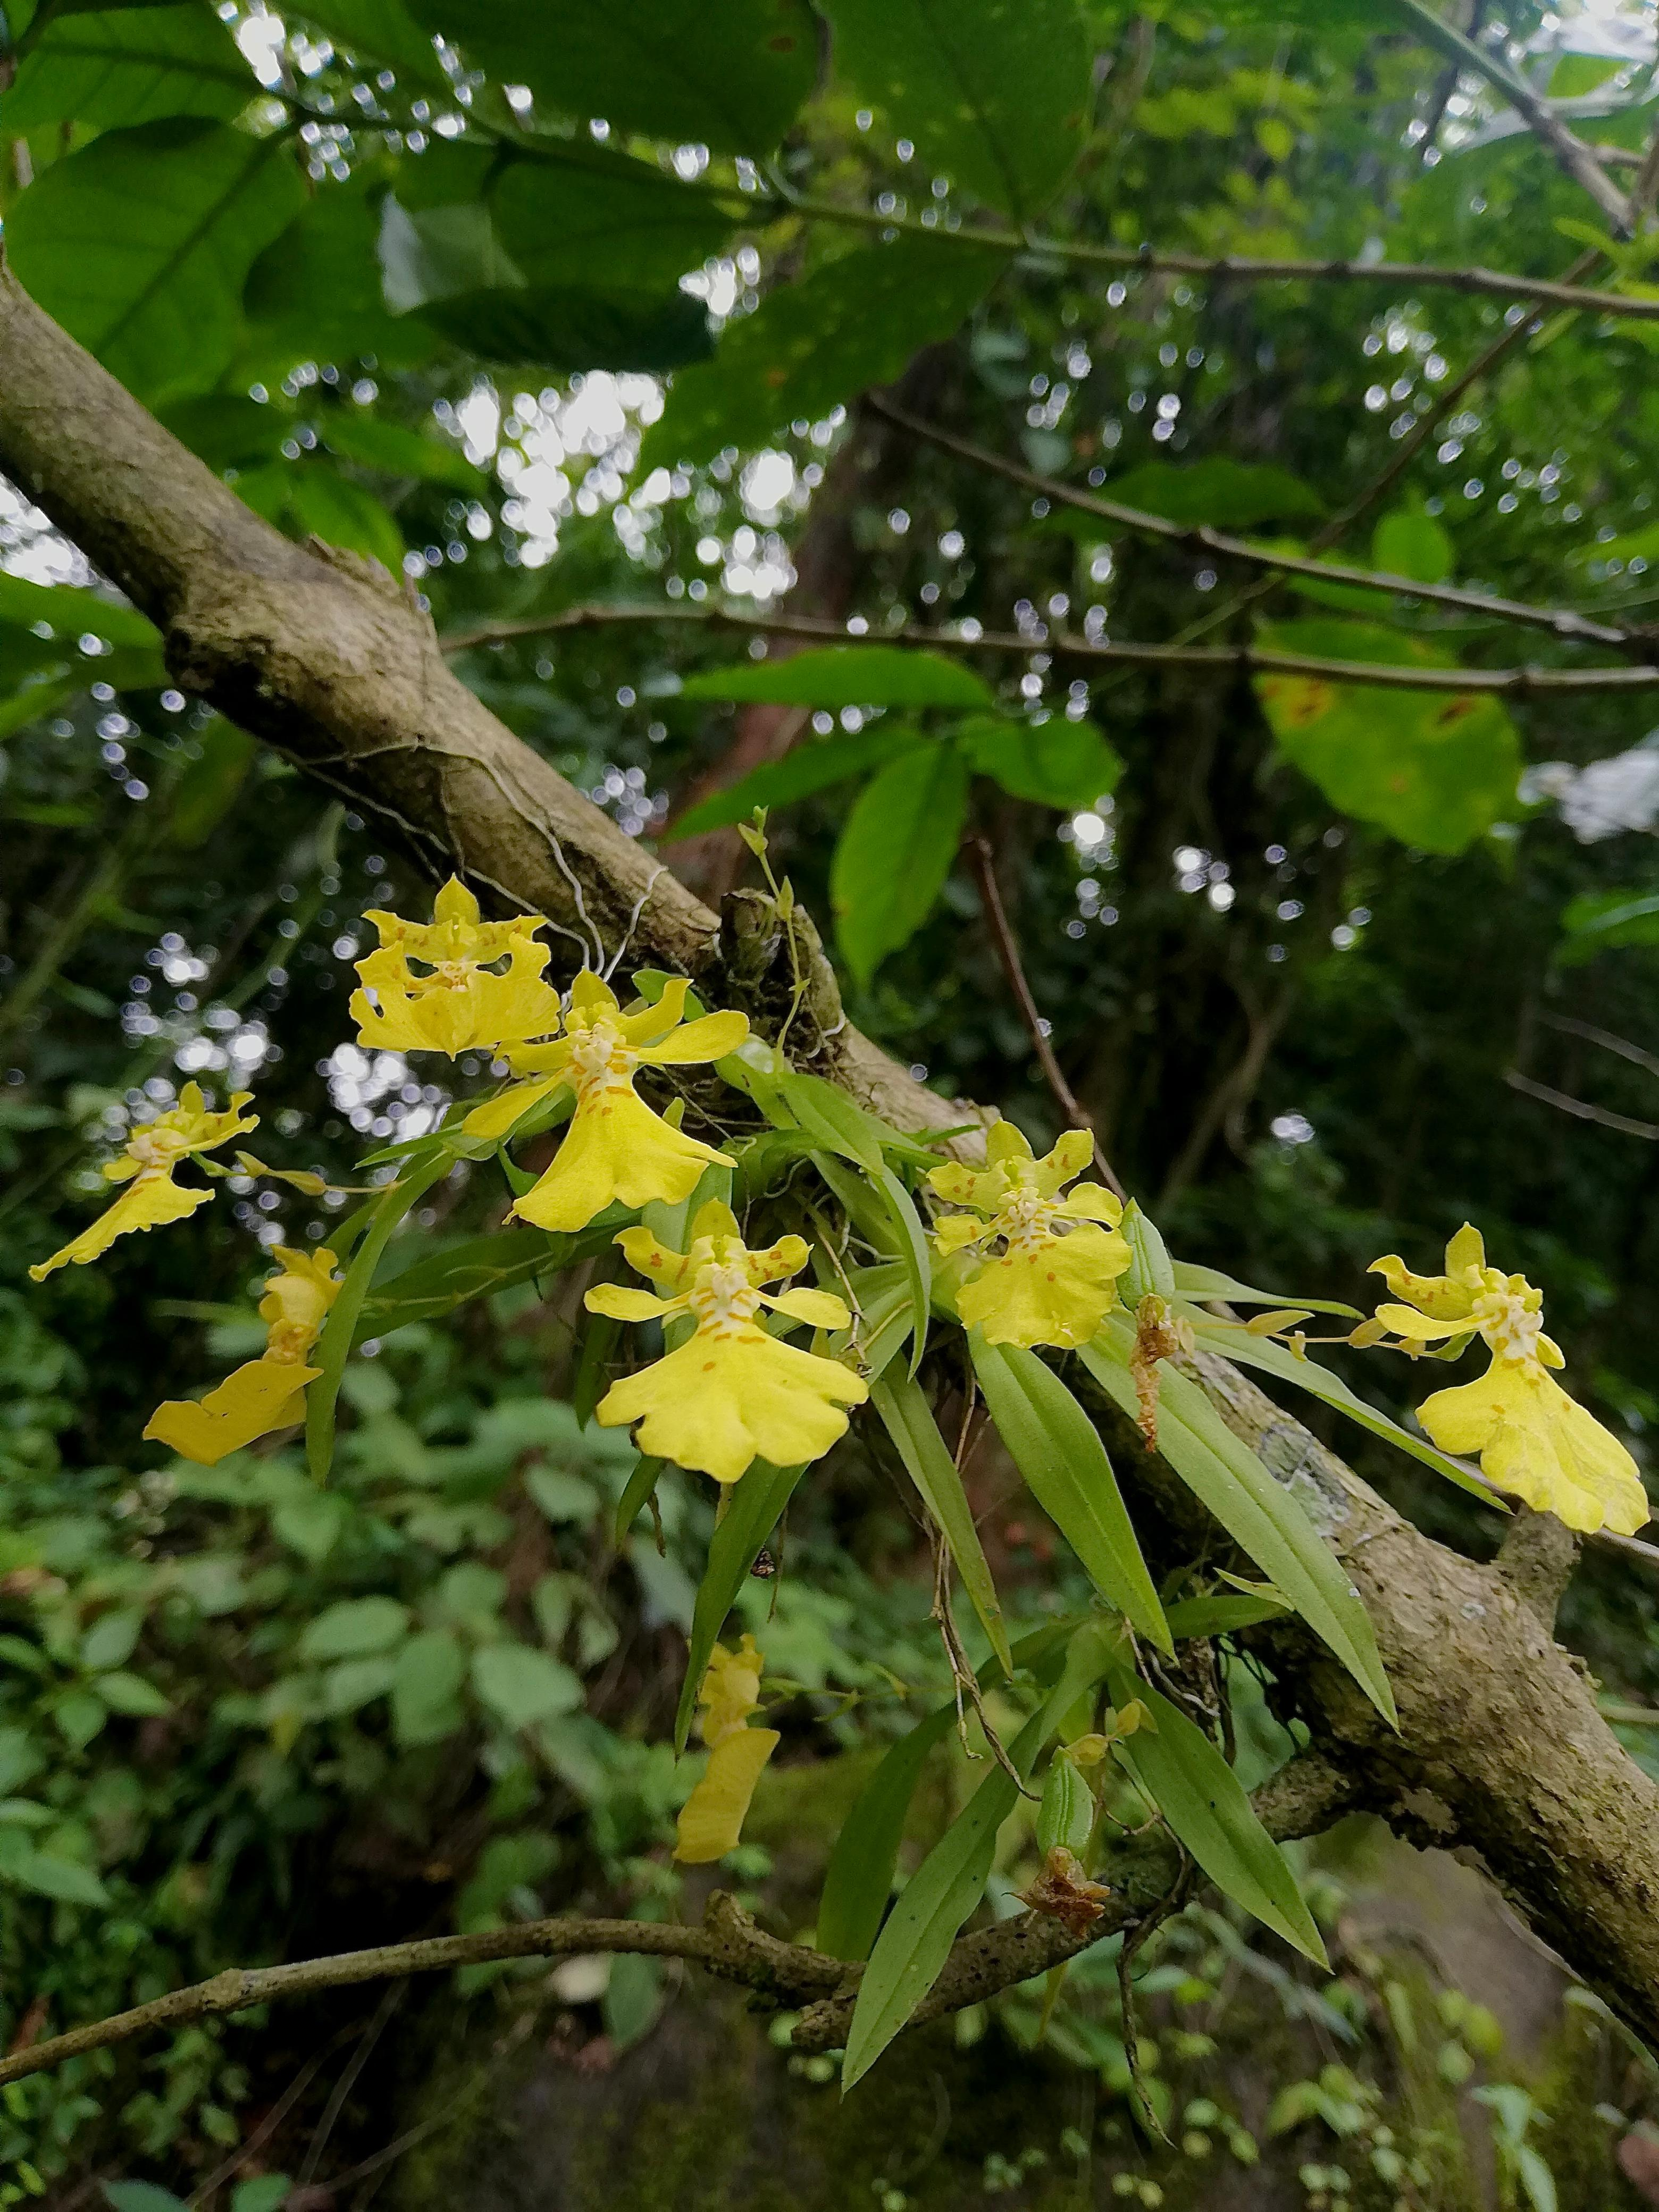
\includegraphics[keepaspectratio]{images/Erycina_crista-galli_Diana_Molina_Ozuma.jpg}}

}

\caption{\emph{Erycina crista-galli}. Foto: Diana Molina Ozuma}

\end{figure}%

En la mayoría de las investigaciones el tamaño de muestra es limitado.
Por lo tanto, es importante considerar si la tasa/transición de
mortalidad es realista y si el tamaño de la muestra es suficiente para
estimar la tasa/transición de mortalidad es de confianza. Si la tasa de
mortalidad es muy baja, cercana a cero o a 100\%, es probable que el
tamaño de la muestra sea demasiado pequeño para estimar la tasa de
mortalidad con precisión. En consecuencia, la tasa de mortalidad
estimada puede estar lejos de la realidad si hubiese tenido un estimado
basado en un \emph{N} más grande.

\begin{center}\rule{0.5\linewidth}{0.5pt}\end{center}

\section{¿Cuáles son los tamaños de muestra típicos en los estudios de
orquídeas?}\label{cuuxe1les-son-los-tamauxf1os-de-muestra-tuxedpicos-en-los-estudios-de-orquuxeddeas}

Usando el artículo de Ticktin y colaboradores (Ticktin et~al., 2020),
vemos algunos de los tamaños de muestra de los estudios de orquídeas
usando MPP. Esta tabla representa solamente parte de los datos en la
publicación. El objetivo es demostrar el tamaño de muestra en algunos de
los estudios de orquídeas. Note que en algunos estudios el tamaño por
etapa es muy pequeño, lo que puede resultar en estimaciones sesgadas de
los parámetros y, a menudo, resultados sin sentido biológico.

\global\setlength{\Oldarrayrulewidth}{\arrayrulewidth}

\global\setlength{\Oldtabcolsep}{\tabcolsep}

\setlength{\tabcolsep}{2pt}

\renewcommand*{\arraystretch}{1.5}



\providecommand{\ascline}[3]{\noalign{\global\arrayrulewidth #1}\arrayrulecolor[HTML]{#2}\cline{#3}}

\begin{longtable*}[c]{ccccc}



\ascline{1.5pt}{666666}{1-5}

\multicolumn{1}{>{}l}{\textcolor[HTML]{000000}{\fontsize{11}{11}\selectfont{Especie}}} & \multicolumn{1}{>{}l}{\textcolor[HTML]{000000}{\fontsize{11}{11}\selectfont{Población}}} & \multicolumn{1}{>{}l}{\textcolor[HTML]{000000}{\fontsize{11}{11}\selectfont{Etapas}}} & \multicolumn{1}{>{}r}{\textcolor[HTML]{000000}{\fontsize{11}{11}\selectfont{Tamaño\ de\ Muestra}}} & \multicolumn{1}{>{}l}{\textcolor[HTML]{000000}{\fontsize{11}{11}\selectfont{Referencia}}} \\

\ascline{1.5pt}{666666}{1-5}\endfirsthead 

\ascline{1.5pt}{666666}{1-5}

\multicolumn{1}{>{}l}{\textcolor[HTML]{000000}{\fontsize{11}{11}\selectfont{Especie}}} & \multicolumn{1}{>{}l}{\textcolor[HTML]{000000}{\fontsize{11}{11}\selectfont{Población}}} & \multicolumn{1}{>{}l}{\textcolor[HTML]{000000}{\fontsize{11}{11}\selectfont{Etapas}}} & \multicolumn{1}{>{}r}{\textcolor[HTML]{000000}{\fontsize{11}{11}\selectfont{Tamaño\ de\ Muestra}}} & \multicolumn{1}{>{}l}{\textcolor[HTML]{000000}{\fontsize{11}{11}\selectfont{Referencia}}} \\

\ascline{1.5pt}{666666}{1-5}\endhead



\multicolumn{1}{>{}l}{\textcolor[HTML]{000000}{\fontsize{11}{11}\selectfont{*Erycina\ crista-galli*}}} & \multicolumn{1}{>{}l}{\textcolor[HTML]{000000}{\fontsize{11}{11}\selectfont{Pop\_1}}} & \multicolumn{1}{>{}l}{\textcolor[HTML]{000000}{\fontsize{11}{11}\selectfont{Plántulas}}} & \multicolumn{1}{>{}r}{\textcolor[HTML]{000000}{\fontsize{11}{11}\selectfont{41}}} & \multicolumn{1}{>{}l}{\textcolor[HTML]{000000}{\fontsize{11}{11}\selectfont{@mondragon2007life}}} \\





\multicolumn{1}{>{}l}{\textcolor[HTML]{000000}{\fontsize{11}{11}\selectfont{}}} & \multicolumn{1}{>{}l}{\textcolor[HTML]{000000}{\fontsize{11}{11}\selectfont{}}} & \multicolumn{1}{>{}l}{\textcolor[HTML]{000000}{\fontsize{11}{11}\selectfont{Juveniles}}} & \multicolumn{1}{>{}r}{\textcolor[HTML]{000000}{\fontsize{11}{11}\selectfont{50}}} & \multicolumn{1}{>{}l}{\textcolor[HTML]{000000}{\fontsize{11}{11}\selectfont{}}} \\





\multicolumn{1}{>{}l}{\textcolor[HTML]{000000}{\fontsize{11}{11}\selectfont{}}} & \multicolumn{1}{>{}l}{\textcolor[HTML]{000000}{\fontsize{11}{11}\selectfont{}}} & \multicolumn{1}{>{}l}{\textcolor[HTML]{000000}{\fontsize{11}{11}\selectfont{Adultos\ 1}}} & \multicolumn{1}{>{}r}{\textcolor[HTML]{000000}{\fontsize{11}{11}\selectfont{221}}} & \multicolumn{1}{>{}l}{\textcolor[HTML]{000000}{\fontsize{11}{11}\selectfont{}}} \\





\multicolumn{1}{>{}l}{\textcolor[HTML]{000000}{\fontsize{11}{11}\selectfont{}}} & \multicolumn{1}{>{}l}{\textcolor[HTML]{000000}{\fontsize{11}{11}\selectfont{}}} & \multicolumn{1}{>{}l}{\textcolor[HTML]{000000}{\fontsize{11}{11}\selectfont{Adultos\ 2}}} & \multicolumn{1}{>{}r}{\textcolor[HTML]{000000}{\fontsize{11}{11}\selectfont{226}}} & \multicolumn{1}{>{}l}{\textcolor[HTML]{000000}{\fontsize{11}{11}\selectfont{}}} \\





\multicolumn{1}{>{}l}{\textcolor[HTML]{000000}{\fontsize{11}{11}\selectfont{*Erycina\ crista-galli*}}} & \multicolumn{1}{>{}l}{\textcolor[HTML]{000000}{\fontsize{11}{11}\selectfont{Pop\_2}}} & \multicolumn{1}{>{}l}{\textcolor[HTML]{000000}{\fontsize{11}{11}\selectfont{Plántulas}}} & \multicolumn{1}{>{}r}{\textcolor[HTML]{000000}{\fontsize{11}{11}\selectfont{4}}} & \multicolumn{1}{>{}l}{\textcolor[HTML]{000000}{\fontsize{11}{11}\selectfont{@mondragon2007life}}} \\





\multicolumn{1}{>{}l}{\textcolor[HTML]{000000}{\fontsize{11}{11}\selectfont{}}} & \multicolumn{1}{>{}l}{\textcolor[HTML]{000000}{\fontsize{11}{11}\selectfont{}}} & \multicolumn{1}{>{}l}{\textcolor[HTML]{000000}{\fontsize{11}{11}\selectfont{Juveniles}}} & \multicolumn{1}{>{}r}{\textcolor[HTML]{000000}{\fontsize{11}{11}\selectfont{32}}} & \multicolumn{1}{>{}l}{\textcolor[HTML]{000000}{\fontsize{11}{11}\selectfont{}}} \\





\multicolumn{1}{>{}l}{\textcolor[HTML]{000000}{\fontsize{11}{11}\selectfont{}}} & \multicolumn{1}{>{}l}{\textcolor[HTML]{000000}{\fontsize{11}{11}\selectfont{}}} & \multicolumn{1}{>{}l}{\textcolor[HTML]{000000}{\fontsize{11}{11}\selectfont{Adultos\ 1}}} & \multicolumn{1}{>{}r}{\textcolor[HTML]{000000}{\fontsize{11}{11}\selectfont{25}}} & \multicolumn{1}{>{}l}{\textcolor[HTML]{000000}{\fontsize{11}{11}\selectfont{}}} \\





\multicolumn{1}{>{}l}{\textcolor[HTML]{000000}{\fontsize{11}{11}\selectfont{}}} & \multicolumn{1}{>{}l}{\textcolor[HTML]{000000}{\fontsize{11}{11}\selectfont{}}} & \multicolumn{1}{>{}l}{\textcolor[HTML]{000000}{\fontsize{11}{11}\selectfont{Adultos\ 2}}} & \multicolumn{1}{>{}r}{\textcolor[HTML]{000000}{\fontsize{11}{11}\selectfont{531}}} & \multicolumn{1}{>{}l}{\textcolor[HTML]{000000}{\fontsize{11}{11}\selectfont{}}} \\





\multicolumn{1}{>{}l}{\textcolor[HTML]{000000}{\fontsize{11}{11}\selectfont{*Euchile\ karwinskii*}}} & \multicolumn{1}{>{}l}{\textcolor[HTML]{000000}{\fontsize{11}{11}\selectfont{Sin\ cosecha}}} & \multicolumn{1}{>{}l}{\textcolor[HTML]{000000}{\fontsize{11}{11}\selectfont{Plántulas}}} & \multicolumn{1}{>{}r}{\textcolor[HTML]{000000}{\fontsize{11}{11}\selectfont{20}}} & \multicolumn{1}{>{}l}{\textcolor[HTML]{000000}{\fontsize{11}{11}\selectfont{@elliott2014demography}}} \\





\multicolumn{1}{>{}l}{\textcolor[HTML]{000000}{\fontsize{11}{11}\selectfont{}}} & \multicolumn{1}{>{}l}{\textcolor[HTML]{000000}{\fontsize{11}{11}\selectfont{}}} & \multicolumn{1}{>{}l}{\textcolor[HTML]{000000}{\fontsize{11}{11}\selectfont{Juveniles\ 1}}} & \multicolumn{1}{>{}r}{\textcolor[HTML]{000000}{\fontsize{11}{11}\selectfont{74}}} & \multicolumn{1}{>{}l}{\textcolor[HTML]{000000}{\fontsize{11}{11}\selectfont{}}} \\





\multicolumn{1}{>{}l}{\textcolor[HTML]{000000}{\fontsize{11}{11}\selectfont{}}} & \multicolumn{1}{>{}l}{\textcolor[HTML]{000000}{\fontsize{11}{11}\selectfont{}}} & \multicolumn{1}{>{}l}{\textcolor[HTML]{000000}{\fontsize{11}{11}\selectfont{Juveniles\ 2}}} & \multicolumn{1}{>{}r}{\textcolor[HTML]{000000}{\fontsize{11}{11}\selectfont{91}}} & \multicolumn{1}{>{}l}{\textcolor[HTML]{000000}{\fontsize{11}{11}\selectfont{}}} \\





\multicolumn{1}{>{}l}{\textcolor[HTML]{000000}{\fontsize{11}{11}\selectfont{}}} & \multicolumn{1}{>{}l}{\textcolor[HTML]{000000}{\fontsize{11}{11}\selectfont{}}} & \multicolumn{1}{>{}l}{\textcolor[HTML]{000000}{\fontsize{11}{11}\selectfont{Adultos}}} & \multicolumn{1}{>{}r}{\textcolor[HTML]{000000}{\fontsize{11}{11}\selectfont{44}}} & \multicolumn{1}{>{}l}{\textcolor[HTML]{000000}{\fontsize{11}{11}\selectfont{}}} \\





\multicolumn{1}{>{}l}{\textcolor[HTML]{000000}{\fontsize{11}{11}\selectfont{*Euchile\ karwinskii*}}} & \multicolumn{1}{>{}l}{\textcolor[HTML]{000000}{\fontsize{11}{11}\selectfont{Con\ cosecha}}} & \multicolumn{1}{>{}l}{\textcolor[HTML]{000000}{\fontsize{11}{11}\selectfont{Plántulas}}} & \multicolumn{1}{>{}r}{\textcolor[HTML]{000000}{\fontsize{11}{11}\selectfont{3}}} & \multicolumn{1}{>{}l}{\textcolor[HTML]{000000}{\fontsize{11}{11}\selectfont{@elliott2014demography}}} \\





\multicolumn{1}{>{}l}{\textcolor[HTML]{000000}{\fontsize{11}{11}\selectfont{}}} & \multicolumn{1}{>{}l}{\textcolor[HTML]{000000}{\fontsize{11}{11}\selectfont{}}} & \multicolumn{1}{>{}l}{\textcolor[HTML]{000000}{\fontsize{11}{11}\selectfont{Juveniles\ 1}}} & \multicolumn{1}{>{}r}{\textcolor[HTML]{000000}{\fontsize{11}{11}\selectfont{26}}} & \multicolumn{1}{>{}l}{\textcolor[HTML]{000000}{\fontsize{11}{11}\selectfont{}}} \\





\multicolumn{1}{>{}l}{\textcolor[HTML]{000000}{\fontsize{11}{11}\selectfont{}}} & \multicolumn{1}{>{}l}{\textcolor[HTML]{000000}{\fontsize{11}{11}\selectfont{}}} & \multicolumn{1}{>{}l}{\textcolor[HTML]{000000}{\fontsize{11}{11}\selectfont{Juveniles\ 2}}} & \multicolumn{1}{>{}r}{\textcolor[HTML]{000000}{\fontsize{11}{11}\selectfont{47}}} & \multicolumn{1}{>{}l}{\textcolor[HTML]{000000}{\fontsize{11}{11}\selectfont{}}} \\





\multicolumn{1}{>{}l}{\textcolor[HTML]{000000}{\fontsize{11}{11}\selectfont{}}} & \multicolumn{1}{>{}l}{\textcolor[HTML]{000000}{\fontsize{11}{11}\selectfont{}}} & \multicolumn{1}{>{}l}{\textcolor[HTML]{000000}{\fontsize{11}{11}\selectfont{Adultos}}} & \multicolumn{1}{>{}r}{\textcolor[HTML]{000000}{\fontsize{11}{11}\selectfont{20}}} & \multicolumn{1}{>{}l}{\textcolor[HTML]{000000}{\fontsize{11}{11}\selectfont{}}} \\





\multicolumn{1}{>{}l}{\textcolor[HTML]{000000}{\fontsize{11}{11}\selectfont{*Lepanthes\ caritensis*}}} & \multicolumn{1}{>{}l}{\textcolor[HTML]{000000}{\fontsize{11}{11}\selectfont{Carite}}} & \multicolumn{1}{>{}l}{\textcolor[HTML]{000000}{\fontsize{11}{11}\selectfont{Plántulas}}} & \multicolumn{1}{>{}r}{\textcolor[HTML]{000000}{\fontsize{11}{11}\selectfont{4}}} & \multicolumn{1}{>{}l}{\textcolor[HTML]{000000}{\fontsize{11}{11}\selectfont{@tremblay1997lepanthes}}} \\





\multicolumn{1}{>{}l}{\textcolor[HTML]{000000}{\fontsize{11}{11}\selectfont{}}} & \multicolumn{1}{>{}l}{\textcolor[HTML]{000000}{\fontsize{11}{11}\selectfont{}}} & \multicolumn{1}{>{}l}{\textcolor[HTML]{000000}{\fontsize{11}{11}\selectfont{Juveniles}}} & \multicolumn{1}{>{}r}{\textcolor[HTML]{000000}{\fontsize{11}{11}\selectfont{54}}} & \multicolumn{1}{>{}l}{\textcolor[HTML]{000000}{\fontsize{11}{11}\selectfont{}}} \\





\multicolumn{1}{>{}l}{\textcolor[HTML]{000000}{\fontsize{11}{11}\selectfont{}}} & \multicolumn{1}{>{}l}{\textcolor[HTML]{000000}{\fontsize{11}{11}\selectfont{}}} & \multicolumn{1}{>{}l}{\textcolor[HTML]{000000}{\fontsize{11}{11}\selectfont{Adulto\ no\ reproductivo}}} & \multicolumn{1}{>{}r}{\textcolor[HTML]{000000}{\fontsize{11}{11}\selectfont{24}}} & \multicolumn{1}{>{}l}{\textcolor[HTML]{000000}{\fontsize{11}{11}\selectfont{}}} \\





\multicolumn{1}{>{}l}{\textcolor[HTML]{000000}{\fontsize{11}{11}\selectfont{}}} & \multicolumn{1}{>{}l}{\textcolor[HTML]{000000}{\fontsize{11}{11}\selectfont{}}} & \multicolumn{1}{>{}l}{\textcolor[HTML]{000000}{\fontsize{11}{11}\selectfont{Adultos}}} & \multicolumn{1}{>{}r}{\textcolor[HTML]{000000}{\fontsize{11}{11}\selectfont{12}}} & \multicolumn{1}{>{}l}{\textcolor[HTML]{000000}{\fontsize{11}{11}\selectfont{}}} \\





\multicolumn{1}{>{}l}{\textcolor[HTML]{000000}{\fontsize{11}{11}\selectfont{*Oncidium\ poikilostalix*}}} & \multicolumn{1}{>{}l}{\textcolor[HTML]{000000}{\fontsize{11}{11}\selectfont{Sin\ cosecha}}} & \multicolumn{1}{>{}l}{\textcolor[HTML]{000000}{\fontsize{11}{11}\selectfont{Etapa\ 1}}} & \multicolumn{1}{>{}r}{\textcolor[HTML]{000000}{\fontsize{11}{11}\selectfont{284}}} & \multicolumn{1}{>{}l}{\textcolor[HTML]{000000}{\fontsize{11}{11}\selectfont{@garcia2017impact}}} \\





\multicolumn{1}{>{}l}{\textcolor[HTML]{000000}{\fontsize{11}{11}\selectfont{}}} & \multicolumn{1}{>{}l}{\textcolor[HTML]{000000}{\fontsize{11}{11}\selectfont{}}} & \multicolumn{1}{>{}l}{\textcolor[HTML]{000000}{\fontsize{11}{11}\selectfont{Etapa\ 2}}} & \multicolumn{1}{>{}r}{\textcolor[HTML]{000000}{\fontsize{11}{11}\selectfont{194}}} & \multicolumn{1}{>{}l}{\textcolor[HTML]{000000}{\fontsize{11}{11}\selectfont{}}} \\





\multicolumn{1}{>{}l}{\textcolor[HTML]{000000}{\fontsize{11}{11}\selectfont{}}} & \multicolumn{1}{>{}l}{\textcolor[HTML]{000000}{\fontsize{11}{11}\selectfont{}}} & \multicolumn{1}{>{}l}{\textcolor[HTML]{000000}{\fontsize{11}{11}\selectfont{Etapa\ 3}}} & \multicolumn{1}{>{}r}{\textcolor[HTML]{000000}{\fontsize{11}{11}\selectfont{270}}} & \multicolumn{1}{>{}l}{\textcolor[HTML]{000000}{\fontsize{11}{11}\selectfont{}}} \\





\multicolumn{1}{>{}l}{\textcolor[HTML]{000000}{\fontsize{11}{11}\selectfont{}}} & \multicolumn{1}{>{}l}{\textcolor[HTML]{000000}{\fontsize{11}{11}\selectfont{}}} & \multicolumn{1}{>{}l}{\textcolor[HTML]{000000}{\fontsize{11}{11}\selectfont{Etapa\ 4}}} & \multicolumn{1}{>{}r}{\textcolor[HTML]{000000}{\fontsize{11}{11}\selectfont{338}}} & \multicolumn{1}{>{}l}{\textcolor[HTML]{000000}{\fontsize{11}{11}\selectfont{}}} \\

\ascline{1.5pt}{666666}{1-5}



\end{longtable*}



\arrayrulecolor[HTML]{000000}

\global\setlength{\arrayrulewidth}{\Oldarrayrulewidth}

\global\setlength{\tabcolsep}{\Oldtabcolsep}

\renewcommand*{\arraystretch}{1}

\begin{center}\rule{0.5\linewidth}{0.5pt}\end{center}

\subsection{Irreducibilidad: cuando faltan transiciones entre
etapas}\label{irreducibilidad-cuando-faltan-transiciones-entre-etapas}

La \emph{irreducibilidad} es un concepto importante en los análisis de
matrices poblacionales. Como lo muestra (Caswell, 1989b) y más
recientemente por (Stott et~al., 2010b), las matrices deben de ser
\emph{irreducibles}. El concepto de \emph{irreducibilidad} está asociado
con el ciclo de vida de la especie y la matriz debe incluir las
transiciones de todas las etapas a todas las demás etapas. En la figura
del ciclo de vida siguiente, faltan dos componentes importantes en la
historia de vida de la especie, ningún juvenil crece para convertirse en
adulto y ninguno de los adultos produce plántulas (semillas que crecen
hasta convertirse en plántulas).

Por tal motivo, la matriz sugiere que los juveniles no crecen para
convertirse en adultos, y todos los juveniles siguen siendo juveniles o
mueren, ya que no hay una flecha que conecte a los juveniles con los
adultos. En tanto que en el caso de los adultos no existe una flecha que
los conecte con las plántulas, lo que sugiere que no hay producción de
nuevas plántulas por parte de los adultos.

\begin{Shaded}
\begin{Highlighting}[]
\NormalTok{Sp1matU\_NT }\OtherTok{\textless{}{-}} \FunctionTok{rbind}\NormalTok{(}
  \FunctionTok{c}\NormalTok{(}\FloatTok{0.0}\NormalTok{, }\FloatTok{0.0}\NormalTok{, }\FloatTok{0.0}\NormalTok{),}
  \FunctionTok{c}\NormalTok{(}\FloatTok{0.5}\NormalTok{, }\FloatTok{0.7}\NormalTok{, }\FloatTok{0.0}\NormalTok{),}
  \FunctionTok{c}\NormalTok{(}\FloatTok{0.0}\NormalTok{, }\FloatTok{0.0}\NormalTok{, }\FloatTok{0.995}\NormalTok{)}
\NormalTok{) }\CommentTok{\# transition matrix}

\NormalTok{Sp1matF }\OtherTok{\textless{}{-}} \FunctionTok{rbind}\NormalTok{(}
  \FunctionTok{c}\NormalTok{(}\FloatTok{0.0}\NormalTok{, }\FloatTok{0.0}\NormalTok{, }\FloatTok{0.0}\NormalTok{),}
  \FunctionTok{c}\NormalTok{(}\FloatTok{0.0}\NormalTok{, }\FloatTok{0.0}\NormalTok{, }\FloatTok{0.0}\NormalTok{),}
  \FunctionTok{c}\NormalTok{(}\FloatTok{0.0}\NormalTok{, }\FloatTok{0.0}\NormalTok{, }\FloatTok{0.0}\NormalTok{)}
\NormalTok{) }\CommentTok{\# fertility matrix}

\NormalTok{Sp1matA\_NT }\OtherTok{=}\NormalTok{ Sp1matU\_NT }\SpecialCharTok{+}\NormalTok{ Sp1matF }\CommentTok{\# TF matrix}

\NormalTok{stages }\OtherTok{\textless{}{-}} \FunctionTok{c}\NormalTok{(}\StringTok{"plantula"}\NormalTok{, }\StringTok{"juvenil"}\NormalTok{, }\StringTok{"adulto"}\NormalTok{)}

\FunctionTok{plot\_life\_cycle}\NormalTok{(Sp1matA\_NT, }\AttributeTok{stages =}\NormalTok{ stages, }\AttributeTok{fontsize =} \DecValTok{0}\NormalTok{)}
\end{Highlighting}
\end{Shaded}

\pandocbounded{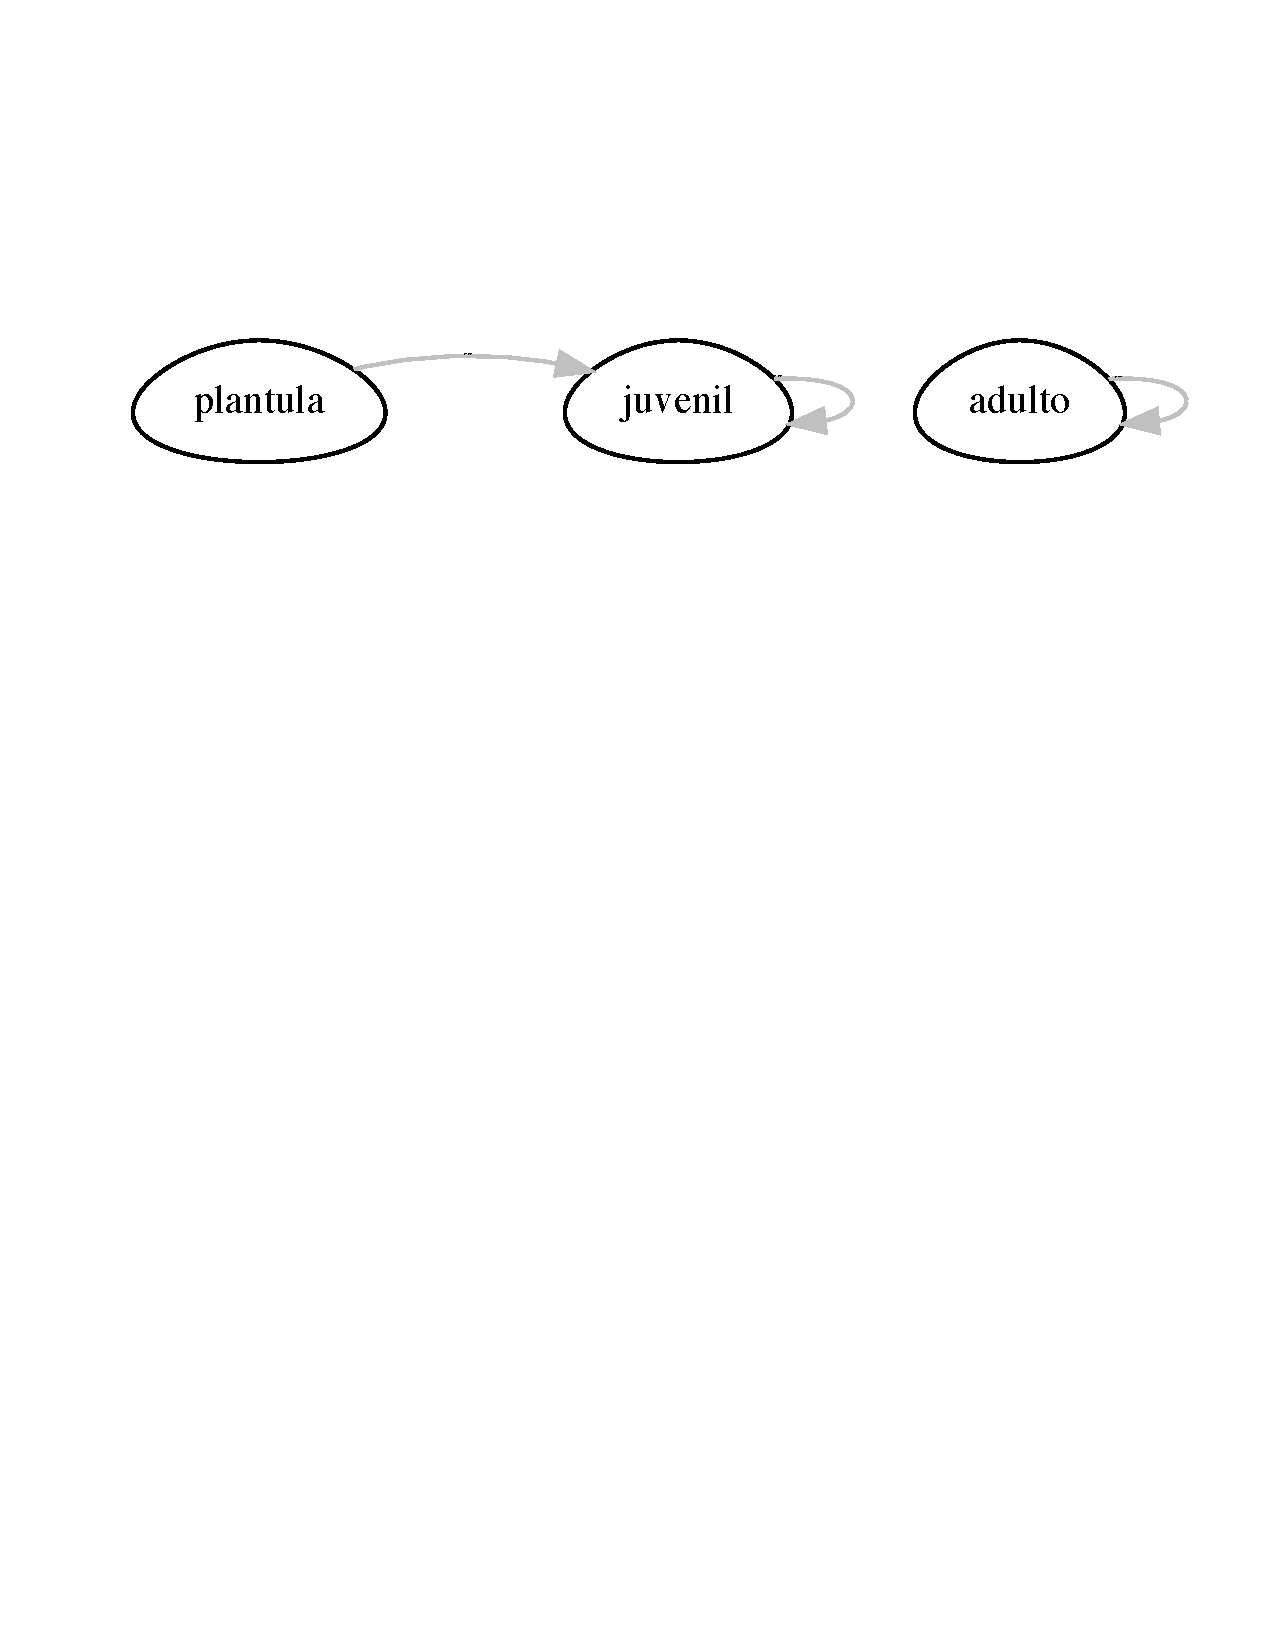
\includegraphics[keepaspectratio]{122-Impacto_de_Datos_sin_Sentido_files/figure-pdf/sin_sentido_6-1.pdf}}

\subsubsection{Función para evaluar si una matriz es
irreducible}\label{funciuxf3n-para-evaluar-si-una-matriz-es-irreducible}

Una manera fácil de determinar si la matriz es irreducible es correr el
siguiente \emph{script} \texttt{isIrreducible} del paquete
\textbf{popdemo}. Tenga en cuenta que, en este caso, el resultado es
\emph{FALSE} para la matriz anterior. Para comparar, si evaluamos la
matriz \textbf{Sp1matA\_2} el resultado es \textbf{TRUE} ya que todas
las etapas pueden llegar a todas las demás etapas. En este caso, la
matriz es irreducible y por tanto cumple con los requisitos necesarios
para muchos de los análisis de matrices poblacionales.

\begin{Shaded}
\begin{Highlighting}[]
\FunctionTok{isIrreducible}\NormalTok{(Sp1matU\_NT) }\CommentTok{\# para la matriz de transición, faltando una etapa de transición y fertilidad}
\end{Highlighting}
\end{Shaded}

\begin{verbatim}
[1] FALSE
\end{verbatim}

\begin{Shaded}
\begin{Highlighting}[]
\FunctionTok{isIrreducible}\NormalTok{(Sp1matA\_NT) }\CommentTok{\# para la matriz TF, falta una etapa de transición}
\end{Highlighting}
\end{Shaded}

\begin{verbatim}
[1] FALSE
\end{verbatim}

\begin{Shaded}
\begin{Highlighting}[]
\CommentTok{\# Ahora considerando Sp1matA\_2}
\CommentTok{\# En esta matriz que incluye todas las transiciones y la fertilidad el resultado es "TRUE"}
\NormalTok{Sp1matA\_2}
\end{Highlighting}
\end{Shaded}

\begin{verbatim}
     [,1] [,2]  [,3]
[1,]  0.0  0.0 1.000
[2,]  0.5  0.3 0.000
[3,]  0.0  0.4 0.995
\end{verbatim}

\begin{Shaded}
\begin{Highlighting}[]
\FunctionTok{isIrreducible}\NormalTok{(Sp1matA\_2)}
\end{Highlighting}
\end{Shaded}

\begin{verbatim}
[1] TRUE
\end{verbatim}

\begin{tcolorbox}[enhanced jigsaw, arc=.35mm, bottomrule=.15mm, bottomtitle=1mm, breakable, colback=white, colbacktitle=quarto-callout-warning-color!10!white, colframe=quarto-callout-warning-color-frame, coltitle=black, left=2mm, leftrule=.75mm, opacityback=0, opacitybacktitle=0.6, rightrule=.15mm, title=\textcolor{quarto-callout-warning-color}{\faExclamationTriangle}\hspace{0.5em}{Cómo detectar y resolver --- matriz reducible}, titlerule=0mm, toprule=.15mm, toptitle=1mm]

\textbf{Detección en R:}

\begin{Shaded}
\begin{Highlighting}[]
\NormalTok{popdemo}\SpecialCharTok{::}\FunctionTok{isIrreducible}\NormalTok{(matA)      }\CommentTok{\# FALSE indica el problema}
\NormalTok{popdemo}\SpecialCharTok{::}\FunctionTok{isErgodic}\NormalTok{(matA)          }\CommentTok{\# complementaria: ¿la población converge?}
\end{Highlighting}
\end{Shaded}

\textbf{Causa típica:} una transición biológicamente posible (juvenil →
adulto, adulto → plántula vía reproducción) tiene valor 0 en la matriz,
ya sea por no haberse observado en el muestreo o por no haber incluido
la fecundidad correctamente en la matriz F.

\textbf{Cómo evitarlo o corregirlo:}

\begin{enumerate}
\def\labelenumi{\arabic{enumi}.}
\tightlist
\item
  Dibujar el gráfico del ciclo de vida y verificar que cada etapa puede
  llegar a cualquier otra etapa por algún camino.
\item
  Si la transición existe biológicamente pero es rara, asignarle un
  valor pequeño positivo (p.~ej., \texttt{1/(N+1)}) en lugar de cero, o
  usar un previo bayesiano.
\item
  Si la transición no existe en la biología (etapas post-reproductivas,
  dispersión unidireccional), reportar la matriz como reducible
  \emph{justificadamente} y elegir métodos compatibles con esta
  estructura (ver capítulo de Propiedades de las matrices).
\end{enumerate}

\end{tcolorbox}

\begin{center}\rule{0.5\linewidth}{0.5pt}\end{center}

\subsection{Ninguna supervivencia}\label{ninguna-supervivencia}

La mortalidad es uno de los estadios del ciclo de vida de cada especie,
pero raramente se añade al diagrama del ciclo de vida, porque es
implícito en los cálculos ya que si restamos 1 a la suma de la columna
de transición de un estadio dado, el resultado será la mortalidad de
dicho estadio. A menudo se observa que la supervivencia de los
individuos más pequeños o la primera etapa del ciclo de vida de una
especie es muy reducida, por lo que la probabilidad de supervivencia es
muy baja. Por ejemplo, la mayoría de las semillas no sobreviven para
germinar. Esta es la norma en las orquídeas donde la producción de
semillas es muy alta, a veces millones de semillas en una cápsula
(Arditti \& Ghani, 2000), pero los porcentajes de germinación en el
campo suelen ser menores. Al momento no conocemos trabajos sistemáticos
evaluando la probabilidad de germinación en orquídeas. Sin embargo, esto
no se limita a las orquídeas, en los árboles se puede observar el mismo
patrón, por ejemplo, en \emph{Nothofagus pumilio} el reclutamiento de
plántulas fue inferior al 1.5 \% (Torres et~al., 2015). En general los
patrones de germinación \emph{in situ} varían por grupos taxonómicos,
distribución y condiciones ecológicas (Iralu, Barbhuyan \& Upadhaya,
2019).

Como es bien conocido en el campo, la germinación de semillas en las
orquídeas no es sencilla ya que depende de la disponibilidad de
micorrizas (Rasmussen, 1995). Si bien existe controversia, hay
especificidad de las orquídeas por ciertas especies de hongos
micorrízicos, ya que hay evidencias de que ciertas especies de orquídeas
presentan dicha especificidad (Balducci, Calevo \& Duffy, 2024), en
tanto que otras no la presentan (Petrolli et~al., 2022), es indiscutible
que para la germinación de las semillas de las orquídeas, las cuales
carecen de endospermo la asociación con un hongo micorrízico es
indispensable para su germinación (Rasmussen et~al., 2015). Pero la
germinación no sólo depende de esta asociación ya que muchas variables
pueden influir incluyendo las condiciones bióticas y abióticas (Callaway
et~al., 2002; Rasmussen et~al., 2015; González-Orellana et~al., 2024).

En el siguiente gráfico del ciclo de vida emergido, se puede observar
que ninguna de las plántulas sobrevive o crece a la siguiente etapa.
Tenga en cuenta que en la primera columna de la matriz de transición
todos los valores son cero. La población puede haber comenzado con
muchas (incluso miles o cientos de miles) de plántulas, pero ninguna
creció hasta convertirse en un juvenil o permaneció como plántula antes
del siguiente muestreo. Esto da como resultado una matriz que es
reducible \emph{isIrreducible} = \emph{FALSE} y por consecuencia no
cumple con los requisitos necesarios para muchos de los análisis de
matrices poblacionales.

\begin{Shaded}
\begin{Highlighting}[]
\NormalTok{Sp1matU\_NS }\OtherTok{\textless{}{-}} \FunctionTok{rbind}\NormalTok{(}
  \FunctionTok{c}\NormalTok{(}\FloatTok{0.0}\NormalTok{, }\FloatTok{0.0}\NormalTok{, }\FloatTok{0.0}\NormalTok{),}
  \FunctionTok{c}\NormalTok{(}\FloatTok{0.0}\NormalTok{, }\FloatTok{0.7}\NormalTok{, }\FloatTok{0.0}\NormalTok{),}
  \FunctionTok{c}\NormalTok{(}\FloatTok{0.0}\NormalTok{, }\FloatTok{0.25}\NormalTok{, }\FloatTok{0.995}\NormalTok{)}
\NormalTok{) }\CommentTok{\# transition matrix}

\NormalTok{Sp1matF }\OtherTok{\textless{}{-}} \FunctionTok{rbind}\NormalTok{(}
  \FunctionTok{c}\NormalTok{(}\FloatTok{0.0}\NormalTok{, }\FloatTok{0.0}\NormalTok{, }\FloatTok{1.0}\NormalTok{),}
  \FunctionTok{c}\NormalTok{(}\FloatTok{0.0}\NormalTok{, }\FloatTok{0.0}\NormalTok{, }\FloatTok{0.0}\NormalTok{),}
  \FunctionTok{c}\NormalTok{(}\FloatTok{0.0}\NormalTok{, }\FloatTok{0.0}\NormalTok{, }\FloatTok{0.0}\NormalTok{)}
\NormalTok{) }\CommentTok{\# fertility matrix}

\NormalTok{Sp1matA\_NS }\OtherTok{=}\NormalTok{ Sp1matU\_NS }\SpecialCharTok{+}\NormalTok{ Sp1matF }\CommentTok{\# TF matrix}

\NormalTok{stages }\OtherTok{\textless{}{-}} \FunctionTok{c}\NormalTok{(}\StringTok{"plantula"}\NormalTok{, }\StringTok{"juvenil"}\NormalTok{, }\StringTok{"adulto"}\NormalTok{)}

\FunctionTok{plot\_life\_cycle}\NormalTok{(Sp1matU\_NS, }\AttributeTok{stages =}\NormalTok{ stages, }\AttributeTok{fontsize =} \DecValTok{0}\NormalTok{)}
\end{Highlighting}
\end{Shaded}

\pandocbounded{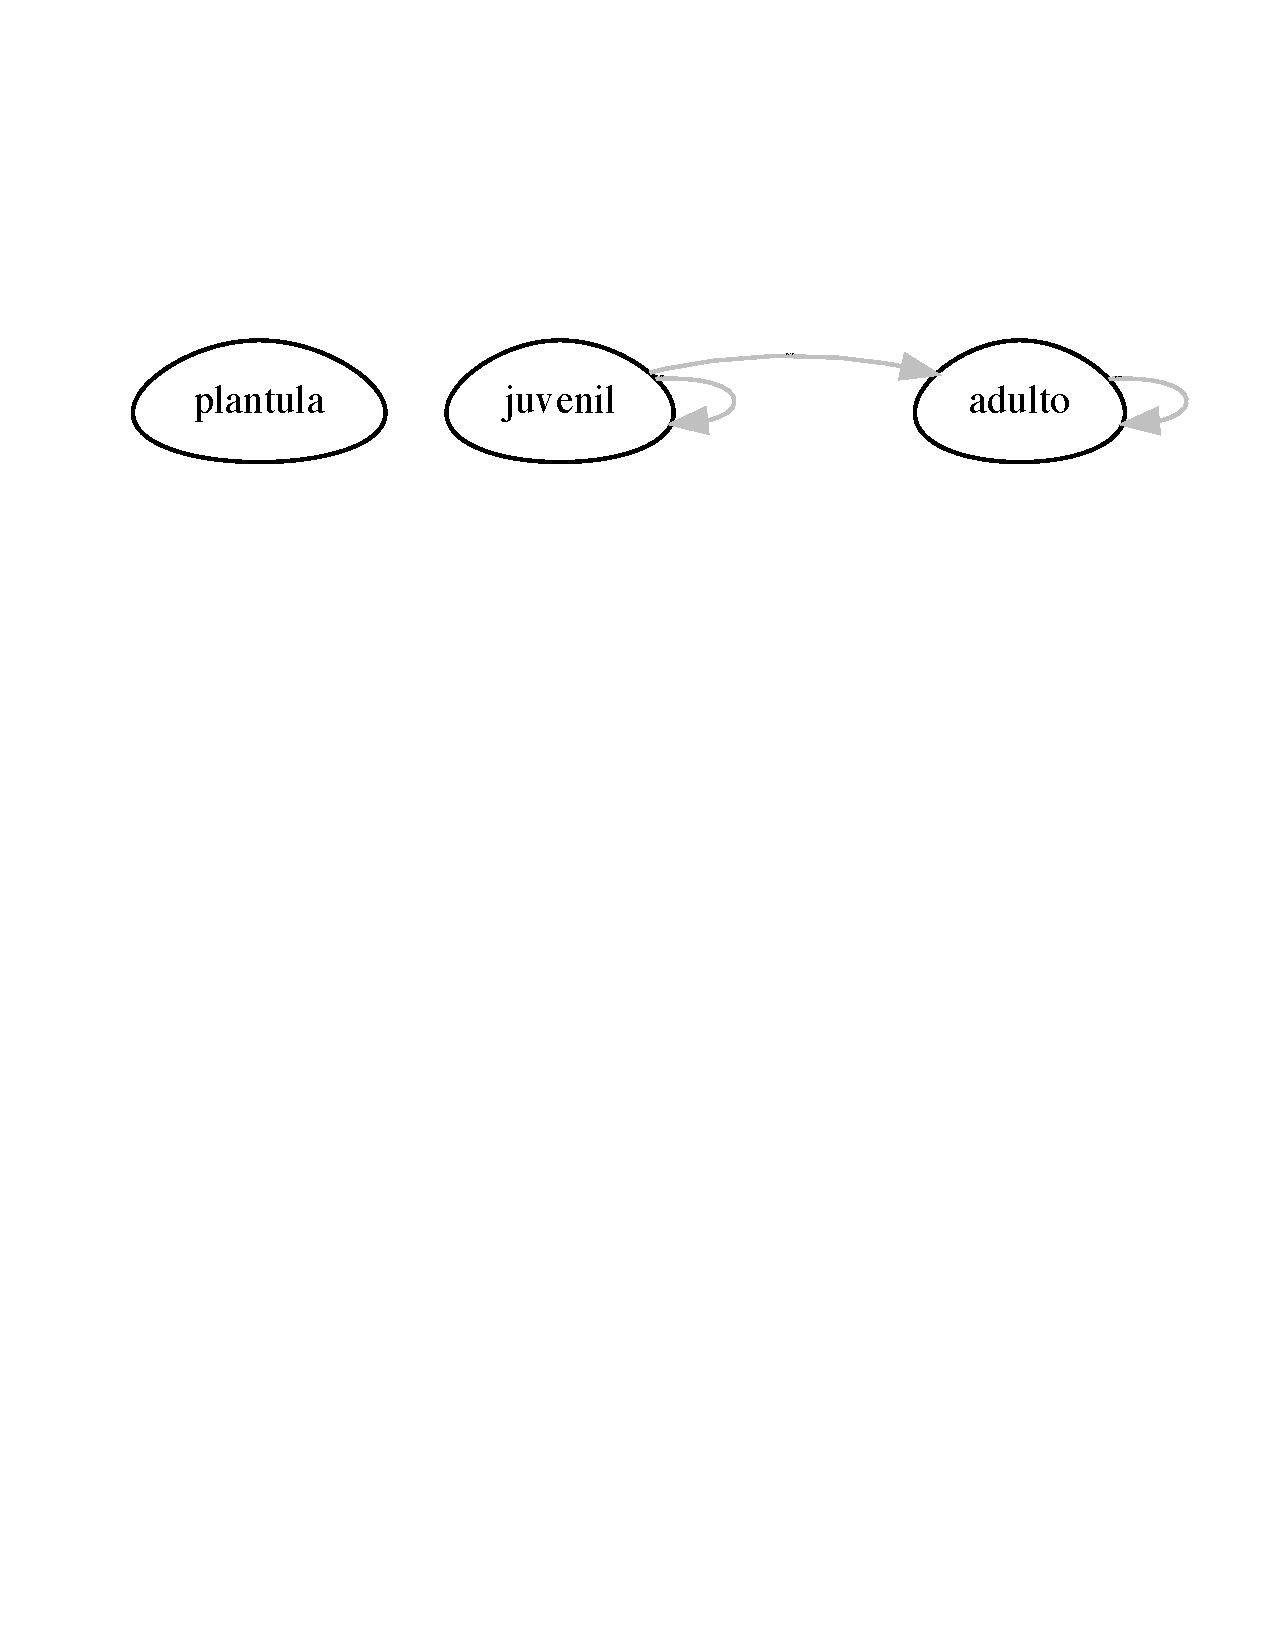
\includegraphics[keepaspectratio]{122-Impacto_de_Datos_sin_Sentido_files/figure-pdf/sin_sentido_8-1.pdf}}

\begin{Shaded}
\begin{Highlighting}[]
\FunctionTok{isIrreducible}\NormalTok{(Sp1matU\_NS)}
\end{Highlighting}
\end{Shaded}

\begin{verbatim}
[1] FALSE
\end{verbatim}

\begin{tcolorbox}[enhanced jigsaw, arc=.35mm, bottomrule=.15mm, bottomtitle=1mm, breakable, colback=white, colbacktitle=quarto-callout-warning-color!10!white, colframe=quarto-callout-warning-color-frame, coltitle=black, left=2mm, leftrule=.75mm, opacityback=0, opacitybacktitle=0.6, rightrule=.15mm, title=\textcolor{quarto-callout-warning-color}{\faExclamationTriangle}\hspace{0.5em}{Cómo detectar y resolver --- sobrevivencia cero en una etapa temprana}, titlerule=0mm, toprule=.15mm, toptitle=1mm]

\textbf{Detección en R:}

\begin{Shaded}
\begin{Highlighting}[]
\FunctionTok{which}\NormalTok{(}\FunctionTok{colSums}\NormalTok{(matU) }\SpecialCharTok{==} \DecValTok{0}\NormalTok{)          }\CommentTok{\# ¿columnas enteras de ceros?}
\end{Highlighting}
\end{Shaded}

\textbf{Causa típica:} la primera etapa (semillas, plántulas) tiene una
probabilidad de germinación o supervivencia genuinamente baja, y
\emph{ningún} individuo de los muestreados sobrevivió al siguiente
censo. El valor observado es 0, pero el valor real no lo es.

\textbf{Cómo evitarlo o corregirlo:}

\begin{enumerate}
\def\labelenumi{\arabic{enumi}.}
\tightlist
\item
  Aumentar el tamaño de muestra de la etapa crítica si es posible.
\item
  Acoplar muestreos \emph{ex situ} (cajas de germinación, paquetes de
  malla) para estimar el reclutamiento con precisión separada del tamaño
  poblacional.
\item
  Usar un previo bayesiano biológicamente informado por la literatura
  (ver capítulo bayesiano y \texttt{raretrans}).
\item
  Si se decide reportar 0, declararlo como un límite inferior y reportar
  el tamaño de muestra que produjo esa estimación.
\end{enumerate}

\end{tcolorbox}

\begin{center}\rule{0.5\linewidth}{0.5pt}\end{center}

\section{Redondeo excesivo de
valores}\label{redondeo-excesivo-de-valores}

Uno de los errores más comunes en la construcción de los elementos de la
matriz es el error de redondeo excesivo u otras estimaciones que dan
como resultado valores de supervivencia superiores a 100\%. Una
estimación de supervivencia mayor a 1.00, genera que de manera
artificial (por un milagro matemático) aumente la cantidad de
individuos, ya que su origen no es debido a la reproducción (sexual u
asexual), si no a un artificio matemático. El estimado de supervivencia
de una etapa siempre tiene que ser menor o igual a 1. Tomemos el ejemplo
del análisis de \emph{Serapias cordigera} (Pellegrino \& Bellusci, 2014)
en donde los autores evaluaron las transiciones entre latencia,
plántulas, roseta vegetativa y floración, en este ejemplo podemos
observar que al sumar los valores de transición de la columna de
plántulas de la matriz SerapiaU, obtenemos un valor de 1.01, lo que
significa que no solamente las plántulas presentan una sobrevivencia
perfecta, que ya vimos que es biológicamente imposible, si no que además
están apareciendo plántulas de la nada (ya que las plántulas son
incapaces de reproducirse sexual o asexualmente y por tanto su entrada
en la matriz de fecundidad-SerapiaF- es cero), que provocan que la
población de plántulas aumente en un 1\% en cada período. Estos valores
de sobrevivencia superiores a 1 son el resultado de errores en la
recolección de datos y/o en el cálculo de la supervivencia de la etapa,
pero más frecuentemente por el redondeo excesivo de los valores de
sobrevivencia calculada al momento de incorporarlos a la matriz, en
donde generalmente sólo se utilizan entre dos y tres decimales.

\begin{Shaded}
\begin{Highlighting}[]
\NormalTok{SerapiaU }\OtherTok{\textless{}{-}} \FunctionTok{rbind}\NormalTok{(}
  \FunctionTok{c}\NormalTok{(}\FloatTok{0.668}\NormalTok{, }\FloatTok{0.122}\NormalTok{, }\FloatTok{0.294}\NormalTok{, }\FloatTok{0.401}\NormalTok{),}
  \FunctionTok{c}\NormalTok{(}\FloatTok{0.128}\NormalTok{, }\FloatTok{0.000}\NormalTok{, }\FloatTok{0.000}\NormalTok{, }\FloatTok{0.000}\NormalTok{),}
  \FunctionTok{c}\NormalTok{(}\FloatTok{0.000}\NormalTok{, }\FloatTok{0.302}\NormalTok{, }\FloatTok{0.453}\NormalTok{, }\FloatTok{0.366}\NormalTok{),}
  \FunctionTok{c}\NormalTok{(}\FloatTok{0.214}\NormalTok{, }\FloatTok{0.364}\NormalTok{, }\FloatTok{0.185}\NormalTok{, }\FloatTok{0.207}\NormalTok{)}
\NormalTok{) }\CommentTok{\# transition matrix}

\FunctionTok{colSums}\NormalTok{(SerapiaU) }\CommentTok{\# la suma de las columnas, nota que la primera columna es mayor de 100\%. }
\end{Highlighting}
\end{Shaded}

\begin{verbatim}
[1] 1.010 0.788 0.932 0.974
\end{verbatim}

\begin{Shaded}
\begin{Highlighting}[]
\NormalTok{SerapiaF }\OtherTok{\textless{}{-}} \FunctionTok{rbind}\NormalTok{(}
  \FunctionTok{c}\NormalTok{(}\FloatTok{0.0}\NormalTok{, }\FloatTok{0.0}\NormalTok{, }\FloatTok{0.0}\NormalTok{, }\FloatTok{0.0}\NormalTok{),}
  \FunctionTok{c}\NormalTok{(}\FloatTok{0.0}\NormalTok{, }\FloatTok{0.0}\NormalTok{, }\FloatTok{0.0}\NormalTok{, }\FloatTok{0.0}\NormalTok{),}
  \FunctionTok{c}\NormalTok{(}\FloatTok{0.0}\NormalTok{, }\FloatTok{0.0}\NormalTok{, }\FloatTok{0.0}\NormalTok{, }\FloatTok{0.0}\NormalTok{),}
  \FunctionTok{c}\NormalTok{(}\FloatTok{0.0}\NormalTok{, }\FloatTok{0.0}\NormalTok{, }\FloatTok{0.0}\NormalTok{, }\FloatTok{0.0}\NormalTok{)}
\NormalTok{) }\CommentTok{\# fertility matrix}

\NormalTok{SerapiaA }\OtherTok{=}\NormalTok{ SerapiaU }\SpecialCharTok{+}\NormalTok{ SerapiaF }\CommentTok{\# TF matrix}

\NormalTok{stages }\OtherTok{\textless{}{-}} \FunctionTok{c}\NormalTok{(}\StringTok{"latente"}\NormalTok{, }\StringTok{"plantulas"}\NormalTok{, }\StringTok{"vegetativa"}\NormalTok{, }\StringTok{"adulto"}\NormalTok{)}

\FunctionTok{plot\_life\_cycle}\NormalTok{(SerapiaA, }\AttributeTok{stages =}\NormalTok{ stages)}
\end{Highlighting}
\end{Shaded}

\pandocbounded{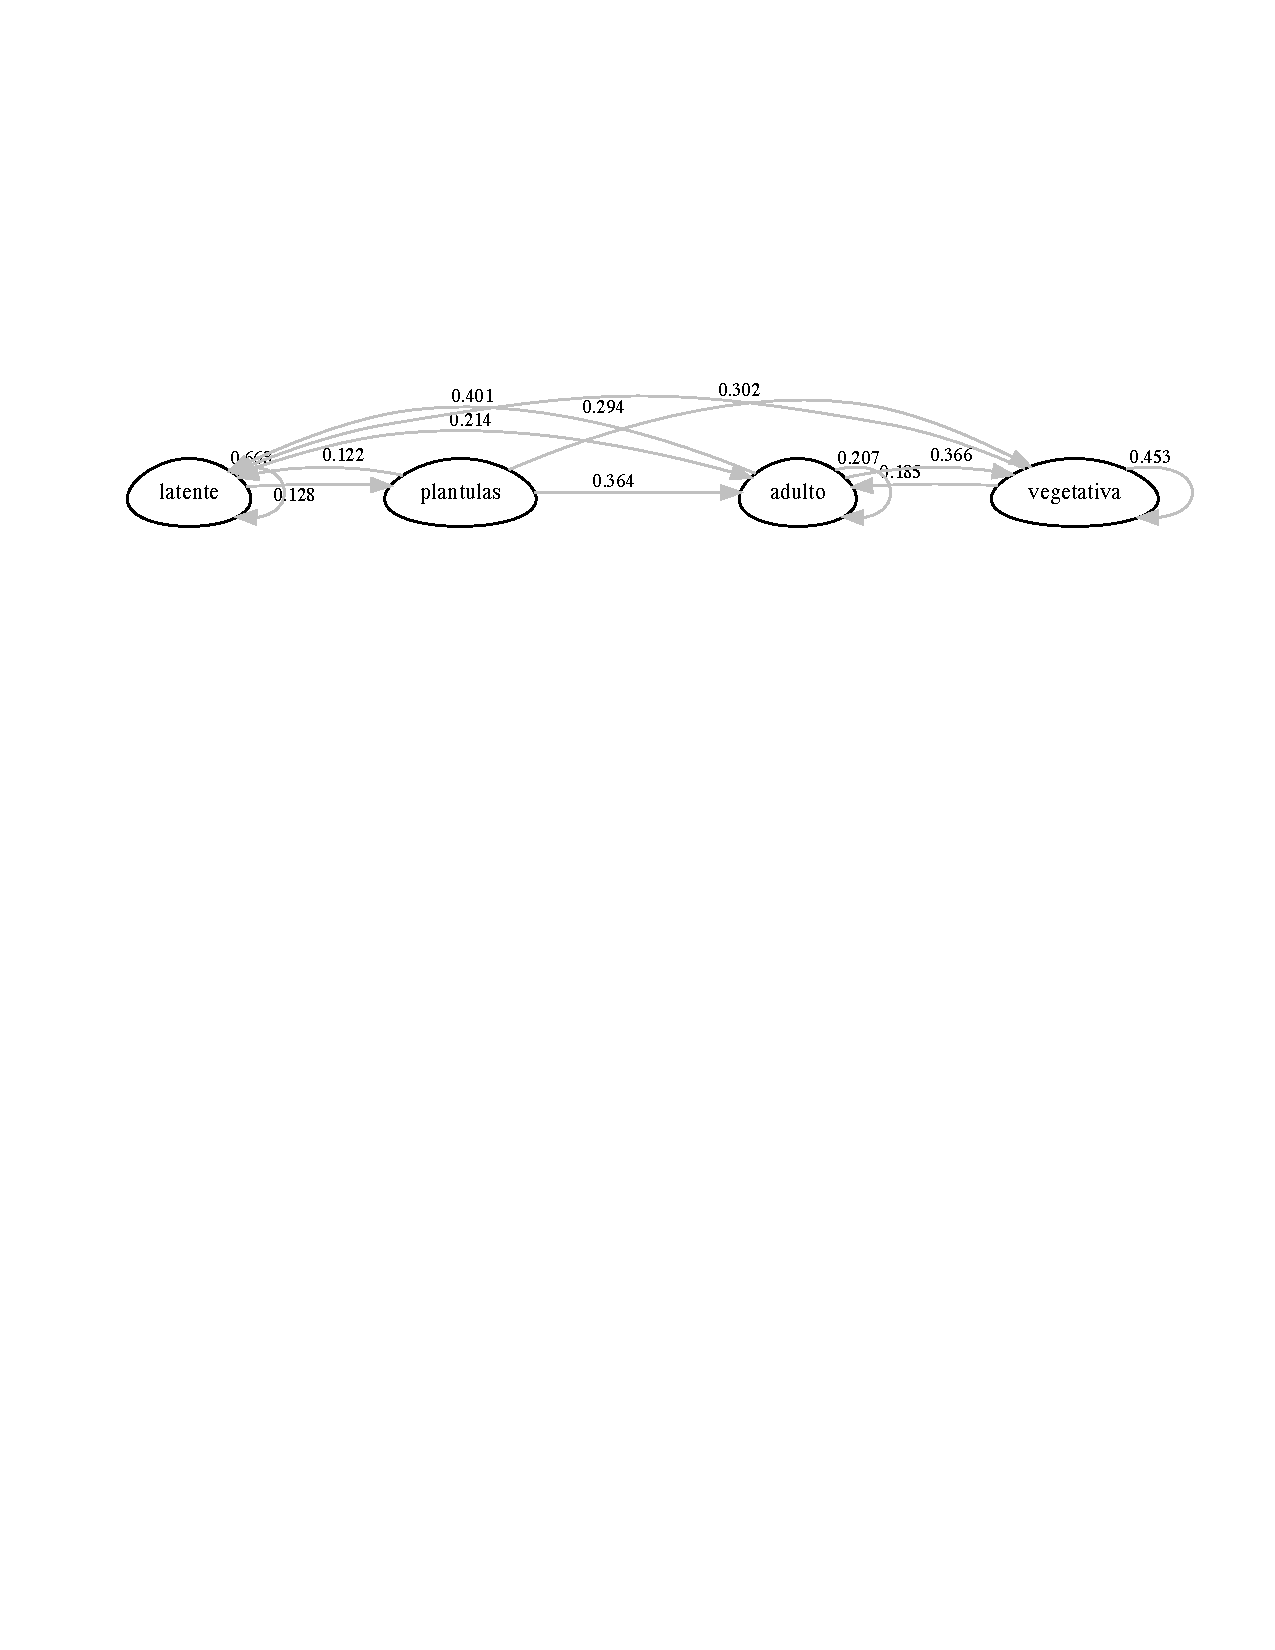
\includegraphics[keepaspectratio]{122-Impacto_de_Datos_sin_Sentido_files/figure-pdf/sin_sentido_9-1.pdf}}

\begin{Shaded}
\begin{Highlighting}[]
\CommentTok{\# Tenga en cuenta que la suma de supervivencia para la etapa inicial es mayor de 1, igual a 1.01}
\end{Highlighting}
\end{Shaded}

\begin{tcolorbox}[enhanced jigsaw, arc=.35mm, bottomrule=.15mm, bottomtitle=1mm, breakable, colback=white, colbacktitle=quarto-callout-warning-color!10!white, colframe=quarto-callout-warning-color-frame, coltitle=black, left=2mm, leftrule=.75mm, opacityback=0, opacitybacktitle=0.6, rightrule=.15mm, title=\textcolor{quarto-callout-warning-color}{\faExclamationTriangle}\hspace{0.5em}{Cómo detectar y resolver --- columna de U que suma más de 1}, titlerule=0mm, toprule=.15mm, toptitle=1mm]

\textbf{Detección en R:}

\begin{Shaded}
\begin{Highlighting}[]
\FunctionTok{which}\NormalTok{(}\FunctionTok{colSums}\NormalTok{(matU) }\SpecialCharTok{\textgreater{}} \DecValTok{1}\NormalTok{)           }\CommentTok{\# ¿qué etapas tienen sobrevivencia \textgreater{} 100\%?}
\FunctionTok{round}\NormalTok{(}\FunctionTok{colSums}\NormalTok{(matU), }\DecValTok{4}\NormalTok{)            }\CommentTok{\# imprime las sumas con 4 decimales}
\end{Highlighting}
\end{Shaded}

\textbf{Causa típica:} redondeo a 2 ó 3 decimales en cada componente de
la transición. Si las cuatro entradas que salen de una etapa se
redondean independientemente, los errores se acumulan en el último
decimal.

\textbf{¿Por qué importa?} Una columna que suma 1.01 en lugar de 1.00
implica un crecimiento artificial del 1 \% por periodo ---en 10
periodos, una sobreestimación de \$\approx\$10 \% de \(\lambda\) que no
proviene de ninguna tasa vital biológica.

\textbf{Cómo evitarlo o corregirlo:}

\begin{enumerate}
\def\labelenumi{\arabic{enumi}.}
\tightlist
\item
  Trabajar con al menos 4--5 decimales en los cálculos intermedios y
  reportar al menos 3 decimales en la matriz final.
\item
  Forzar la consistencia: calcular
  \texttt{mortalidad\ \textless{}-\ 1\ -\ colSums(matU)} y verificar que
  es no-negativa.
\item
  Si la suma sigue excediendo 1, regresar al paso de cálculo de las
  tasas vitales ---no es un problema de redondeo sino de doble conteo
  (un mismo evento entró en dos celdas).
\end{enumerate}

\end{tcolorbox}

\begin{center}\rule{0.5\linewidth}{0.5pt}\end{center}

\section{Estimaciones de fertilidad y ciclo de
vida}\label{estimaciones-de-fertilidad-y-ciclo-de-vida}

La fecundidad influye considerablemente sobre los resultados de los
modelos. Es por ello que cometer errores en la incorporación de valores,
tanto en el ciclo de vida como en las matrices, puede dar lugar a
interpretaciones sin sentido biológico. Por esa razón, en esta sección
mostramos algunos ejemplos de errores al incorporar la fecundidad en el
ciclo de vida y la matriz, y los problemas que generan. Vea el
\hyperref[MatricesF]{capítulo de Fecundidad} para más detalles.

\subsection{Ciclo de vida y etapa de fertilidad
incorrectos}\label{ciclo-de-vida-y-etapa-de-fertilidad-incorrectos}

Suponga que tiene una especie en la que modela el ciclo de vida con los
siguientes estadios: plántula, juvenil y adulto, en donde la fecundidad
se calcula con base en el número de semillas producidas por un adulto
(número medio de semillas por adulto). Después de analizar los datos y
calcular los valores de transición (Sp1matU), se determinó que el número
medio de semillas producido por adulto es 1100, a partir del cual se
construyó la matriz de fecundidad (Sp1matF). Si agregamos a la matriz de
transición la matriz de fertilidad, y a continuación evaluamos el valor
de lambda y graficamos el crecimiento de la población con la función
\emph{proyect}, tenemos un valor de lambda de 4.93 y después de tan solo
5 períodos de tiempo, el número de adultos supera los 250,000
individuos!!! Por consecuencia, la estimación de la tasa de crecimiento
de la población sería incorrecta y engañosa, donde 30\% de 11,000
semillas llegan a ser plántulas, un total de 3,300 plántulas!!!

Este error es el resultado del cálculo de la fecundidad, que debiera ser
estimada con base en la primera etapa de la matriz, en este caso la
etapa de plántula. Por lo tanto, la esquina superior derecha de la
matriz de fertilidad no debe ser la \textbf{cantidad media de semillas}
por planta, sino la \textbf{cantidad media de semillas que transitan a
plántulas} producidas por una planta adulta. Recuerde que el número de
semillas que llegan a plántula, son el resultado de múltiples factores;
por ejemplo el porcentaje de viabilidad de las semillas por adulto, el
porcentaje de semillas que arriban a un micro nicho propicio, el
porcentaje de semillas que germinan y el porcentaje de sobrevivencia de
las plántulas hasta el momento del muestreo, en donde se contabiliza el
número de nuevas plántulas reclutadas. Por consecuencia el valor de
esfuerzo reproductivo que entra en la matriz es condicional a todas
estas condiciones.

\begin{Shaded}
\begin{Highlighting}[]
\NormalTok{Sp1matU\_Fert }\OtherTok{\textless{}{-}} \FunctionTok{rbind}\NormalTok{(}
  \FunctionTok{c}\NormalTok{(}\FloatTok{0.0}\NormalTok{, }\FloatTok{0.0}\NormalTok{, }\FloatTok{0.0}\NormalTok{),}
  \FunctionTok{c}\NormalTok{(}\FloatTok{0.3}\NormalTok{, }\FloatTok{0.7}\NormalTok{, }\FloatTok{0.0}\NormalTok{),}
  \FunctionTok{c}\NormalTok{(}\FloatTok{0.0}\NormalTok{, }\FloatTok{0.25}\NormalTok{, }\FloatTok{0.995}\NormalTok{)}
\NormalTok{) }\CommentTok{\# matriz de transición}

\NormalTok{Sp1matF }\OtherTok{\textless{}{-}} \FunctionTok{rbind}\NormalTok{(}
  \FunctionTok{c}\NormalTok{(}\FloatTok{0.0}\NormalTok{, }\FloatTok{0.0}\NormalTok{, }\FloatTok{1100.0}\NormalTok{),}
  \FunctionTok{c}\NormalTok{(}\FloatTok{0.0}\NormalTok{, }\FloatTok{0.0}\NormalTok{, }\FloatTok{0.0}\NormalTok{),}
  \FunctionTok{c}\NormalTok{(}\FloatTok{0.0}\NormalTok{, }\FloatTok{0.0}\NormalTok{, }\FloatTok{0.0}\NormalTok{)}
\NormalTok{) }\CommentTok{\# matriz de fertilidad}

\NormalTok{Sp1matA\_Fert }\OtherTok{=}\NormalTok{ Sp1matU\_Fert }\SpecialCharTok{+}\NormalTok{ Sp1matF }\CommentTok{\# TF matriz combinada: matA = matU + matF}

\NormalTok{stages }\OtherTok{\textless{}{-}} \FunctionTok{c}\NormalTok{(}\StringTok{"plantula"}\NormalTok{, }\StringTok{"juvenil"}\NormalTok{, }\StringTok{"adulto"}\NormalTok{)}

\FunctionTok{lambda}\NormalTok{(Sp1matA\_Fert)}
\end{Highlighting}
\end{Shaded}

\begin{verbatim}
[1] 4.937718
\end{verbatim}

\begin{Shaded}
\begin{Highlighting}[]
\CommentTok{\# El cambio de tamaño de la población en 5 periodos de tiempo}
\NormalTok{n}
\end{Highlighting}
\end{Shaded}

\begin{verbatim}
[1] 50 50 50
\end{verbatim}

\begin{Shaded}
\begin{Highlighting}[]
\NormalTok{pr }\OtherTok{\textless{}{-}} \FunctionTok{project}\NormalTok{(Sp1matA\_Fert, }\AttributeTok{vector =} \StringTok{"n"}\NormalTok{, }\AttributeTok{time =} \DecValTok{5}\NormalTok{)}
\FunctionTok{plot}\NormalTok{(pr) }\CommentTok{\# Nota que después de solamente 5 años ya la población aumentó a 250,000 individuos}
\end{Highlighting}
\end{Shaded}

\pandocbounded{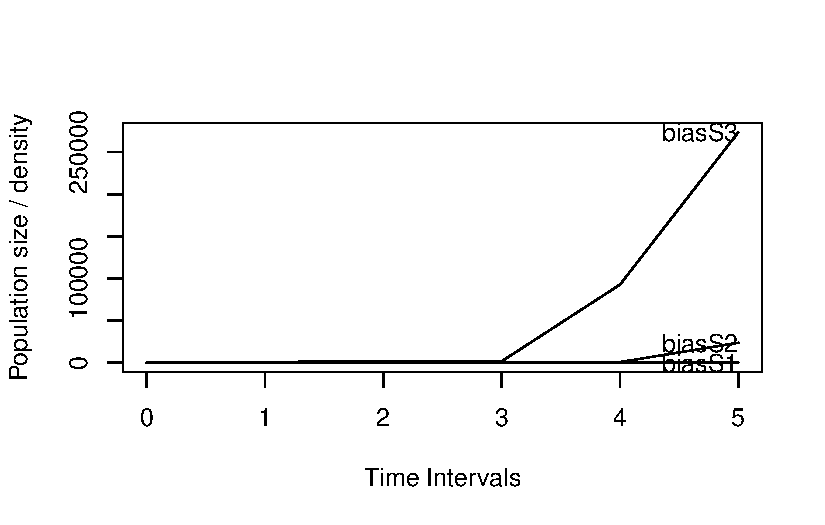
\includegraphics[keepaspectratio]{122-Impacto_de_Datos_sin_Sentido_files/figure-pdf/sin_sentido_10-1.pdf}}

\begin{tcolorbox}[enhanced jigsaw, arc=.35mm, bottomrule=.15mm, bottomtitle=1mm, breakable, colback=white, colbacktitle=quarto-callout-warning-color!10!white, colframe=quarto-callout-warning-color-frame, coltitle=black, left=2mm, leftrule=.75mm, opacityback=0, opacitybacktitle=0.6, rightrule=.15mm, title=\textcolor{quarto-callout-warning-color}{\faExclamationTriangle}\hspace{0.5em}{Cómo detectar y resolver --- fecundidad sobreestimada en la celda
equivocada}, titlerule=0mm, toprule=.15mm, toptitle=1mm]

\textbf{Detección:} en la matriz de fecundidad, la celda superior
derecha contiene un número muy grande (cientos o miles) y produce
\(\lambda\) irreal (p.~ej. \textgreater2 en una especie longeva).
Compare el reclutamiento real anual a la primera etapa con el valor en
la matriz.

\textbf{Causa típica:} se anotó el número medio de \textbf{semillas
producidas por adulto}, sin multiplicar por las probabilidades
concatenadas de viabilidad, dispersión a un micrositio favorable,
germinación y sobrevivencia hasta el primer censo.

\textbf{Cómo evitarlo o corregirlo:}

\begin{enumerate}
\def\labelenumi{\arabic{enumi}.}
\tightlist
\item
  La entrada \(f_{1,k}\) debe ser el número de \textbf{plántulas
  observadas reclutándose por adulto} (la primera etapa del modelo), no
  el número de semillas producidas.
\item
  Documente explícitamente cómo se calculó la fecundidad ---ya sea
  contando reclutas directamente o multiplicando
  \(\text{semillas} \times P_{\text{viabilidad}} \times P_{\text{germinación}} \times P_{\text{sobrevivencia plántula}}\)
  (ver el \hyperref[MatricesF]{capítulo de Fecundidad}).
\item
  Especifique el tipo de censo (pre- o post-reproductivo) y si el modelo
  es birth-flow o birth-pulse (ver el \hyperref[protocolo]{protocolo
  estandarizado del capítulo 121}).
\item
  Si quiere modelar la cadena completa, agregue una etapa de semillas
  explícita ---pero entonces debe reportar la transición semilla →
  plántula, lo que en orquídeas es un dato muy difícil de obtener.
\end{enumerate}

\end{tcolorbox}

\begin{center}\rule{0.5\linewidth}{0.5pt}\end{center}

\subsection{Añadir una etapa de
semillas}\label{auxf1adir-una-etapa-de-semillas}

Si deseamos agregar una etapa de semilla a nuestro modelo, debemos
incluir la etapa en nuestro modelo y crear una matriz con una nueva
etapa \emph{semilla}, para lo cual será necesario tener una estimación
del número de semillas que germinan y se convierten en plántulas para
poder calcular la transición de semillas a plántulas de nuestro modelo.
En el caso de las orquídeas, dicha estimación es bastante difícil de
lograr ya que las semillas de las orquídeas, debido a su tamaño
minúsculo, son difíciles de seguir en la naturaleza. Aunque existen
métodos para seguir las semillas como el de paquetes de malla de
fitoplancton donde uno añade las semillas para monitorear esa etapa
(Rasmussen \& Whigham, 1993; Batty et~al., 2006; Shao, Jacquemyn \&
Selosse, 2024) o algún método de huella genética para determinar la
procedencia de las plántulas, que nos pueden ayudar a tener una
estimación de esta transición, esta será incorrecta la mayoría de las
veces, ya que en el caso de los paquetes de semillas se estará
sobreestimando la transición ya que no se estaría considerando la
pérdida de semillas por dispersión, en tanto que en el método de huella
genética es muy probable que se subestime la transición ya que es muy
difícil encontrar las plántulas en campo, sobre todo en orquídea
epifitas. Por lo tanto, la estimación de la fertilidad en las orquídeas
es un desafío y requiere un muestreo y análisis cuidadoso.

\begin{Shaded}
\begin{Highlighting}[]
\NormalTok{Sp1matU\_Fert2 }\OtherTok{\textless{}{-}} \FunctionTok{rbind}\NormalTok{(}
  \FunctionTok{c}\NormalTok{(}\FloatTok{0.0}\NormalTok{, }\FloatTok{0.0}\NormalTok{, }\FloatTok{0.0}\NormalTok{, }\FloatTok{0.0}\NormalTok{),}
  \FunctionTok{c}\NormalTok{(}\FloatTok{0.0001}\NormalTok{, }\FloatTok{0.0}\NormalTok{, }\FloatTok{0.0}\NormalTok{, }\FloatTok{0.0}\NormalTok{),}
  \FunctionTok{c}\NormalTok{(}\FloatTok{0.0}\NormalTok{, }\FloatTok{0.3}\NormalTok{, }\FloatTok{0.7}\NormalTok{, }\FloatTok{0.0}\NormalTok{),}
  \FunctionTok{c}\NormalTok{(}\FloatTok{0.0}\NormalTok{, }\FloatTok{0.0}\NormalTok{, }\FloatTok{0.25}\NormalTok{, }\FloatTok{0.995}\NormalTok{)}
\NormalTok{) }\CommentTok{\# transition matrix}

\NormalTok{Sp1matF2 }\OtherTok{\textless{}{-}} \FunctionTok{rbind}\NormalTok{(}
  \FunctionTok{c}\NormalTok{(}\FloatTok{0.0}\NormalTok{, }\FloatTok{0.0}\NormalTok{, }\FloatTok{0.0}\NormalTok{, }\FloatTok{1100.0}\NormalTok{),}
  \FunctionTok{c}\NormalTok{(}\FloatTok{0.0}\NormalTok{, }\FloatTok{0.0}\NormalTok{, }\FloatTok{0.0}\NormalTok{, }\FloatTok{0.0}\NormalTok{),}
  \FunctionTok{c}\NormalTok{(}\FloatTok{0.0}\NormalTok{, }\FloatTok{0.0}\NormalTok{, }\FloatTok{0.0}\NormalTok{, }\FloatTok{0.0}\NormalTok{),}
  \FunctionTok{c}\NormalTok{(}\FloatTok{0.0}\NormalTok{, }\FloatTok{0.0}\NormalTok{, }\FloatTok{0.0}\NormalTok{, }\FloatTok{0.0}\NormalTok{)}
\NormalTok{) }\CommentTok{\# fertility matrix}

\NormalTok{Sp1matA\_Fert2 }\OtherTok{=}\NormalTok{ Sp1matU\_Fert2 }\SpecialCharTok{+}\NormalTok{ Sp1matF2 }\CommentTok{\# TF matrix}

\NormalTok{stages }\OtherTok{\textless{}{-}} \FunctionTok{c}\NormalTok{(}\StringTok{"semillas"}\NormalTok{, }\StringTok{"plantula"}\NormalTok{, }\StringTok{"juvenil"}\NormalTok{, }\StringTok{"adulto"}\NormalTok{)}

\FunctionTok{plot\_life\_cycle}\NormalTok{(Sp1matA\_Fert2, }\AttributeTok{stages =}\NormalTok{ stages)}
\end{Highlighting}
\end{Shaded}

\pandocbounded{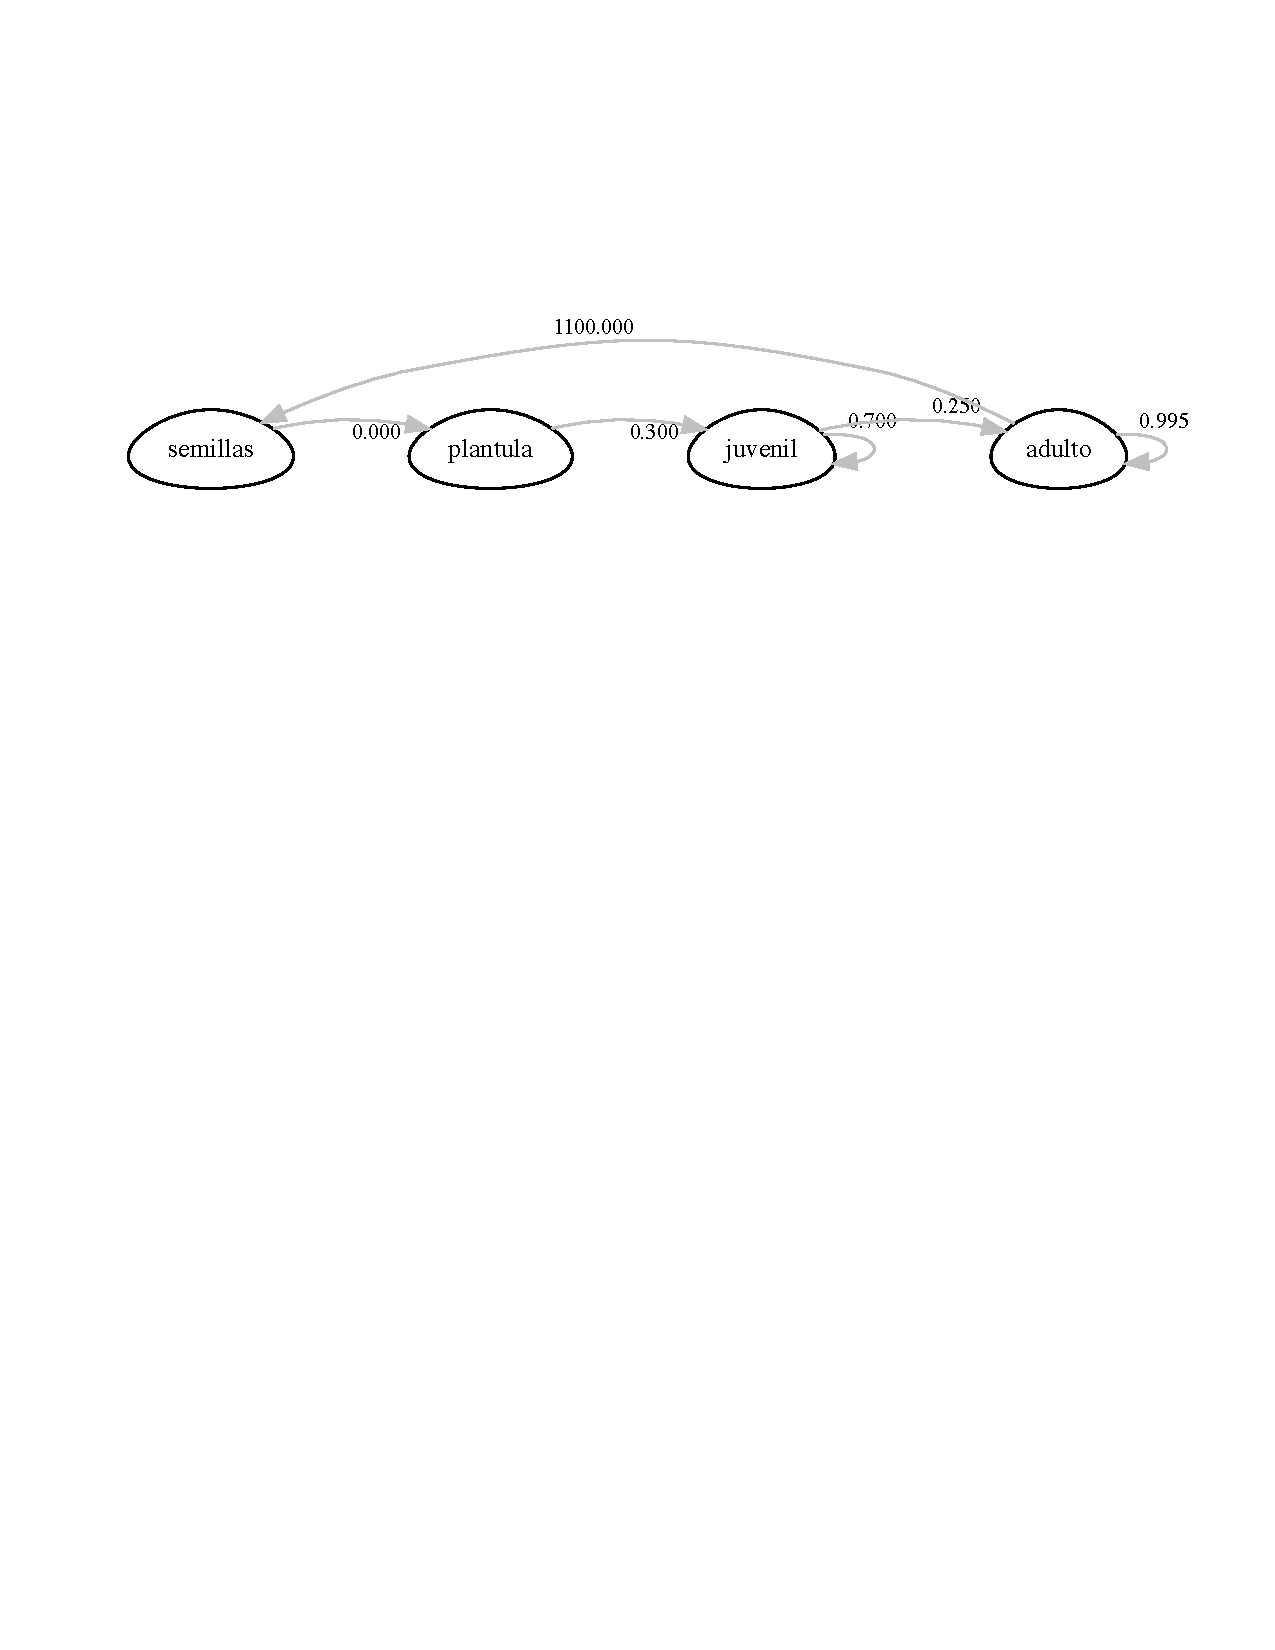
\includegraphics[keepaspectratio]{122-Impacto_de_Datos_sin_Sentido_files/figure-pdf/sin_sentido_11-1.pdf}}

\begin{Shaded}
\begin{Highlighting}[]
\FunctionTok{lambda}\NormalTok{(Sp1matA\_Fert2)}
\end{Highlighting}
\end{Shaded}

\begin{verbatim}
[1] 1.019805
\end{verbatim}

\begin{Shaded}
\begin{Highlighting}[]
\CommentTok{\# show change in population size}
\NormalTok{pr }\OtherTok{\textless{}{-}} \FunctionTok{project}\NormalTok{(Sp1matA\_Fert2, }\AttributeTok{vector =} \StringTok{"n"}\NormalTok{, }\AttributeTok{time =} \DecValTok{5}\NormalTok{)}
\FunctionTok{plot}\NormalTok{(pr) }\CommentTok{\# Note that now the number of adults did not increase to the level of the previous model}
\end{Highlighting}
\end{Shaded}

\pandocbounded{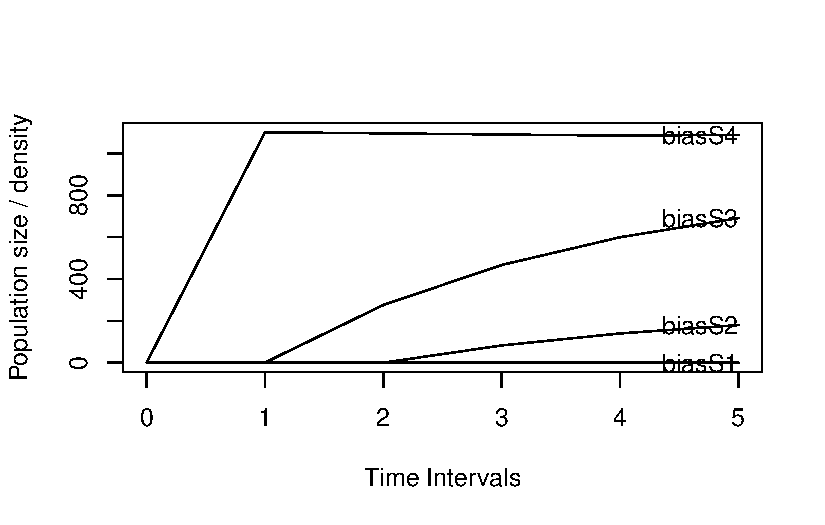
\includegraphics[keepaspectratio]{122-Impacto_de_Datos_sin_Sentido_files/figure-pdf/sin_sentido_11-2.pdf}}

\begin{center}\rule{0.5\linewidth}{0.5pt}\end{center}

\subsection{Semillas latentes}\label{semillas-latentes}

En el ejemplo anterior no hemos incluido una etapa de latencia de
semillas. En otras palabras: ¿las semillas de orquídeas pueden
sobrevivir por un periodo de tiempo largo? Esto sería tener un banco de
semillas. ¿O las semillas, si no germinan el primer año, mueren? En
muchas especies de plantas, las semillas pueden permanecer latentes
durante uno o más años. No se sabe si las semillas de las orquídeas
están inactivas durante mucho tiempo (Gale et~al., 2010), excepto para
algunas especies que han demostrado que las semillas aún están vivas
después de varios años en el suelo usando la prueba de tinción de
tetrazolio (Rasmussen \& Whigham, 1993; Whigham et~al., 2006). Es
posible que las orquídeas terrestres tengan un banco de semillas, pero
no se ha demostrado que las orquídeas epífitas tengan un banco de
semillas. Por lo tanto, si se desea incluir una etapa de latencia de
semillas en el modelo, es necesario tener una estimación del número de
semillas que permanecen latentes y que pueden germinar en el futuro.

\begin{center}\rule{0.5\linewidth}{0.5pt}\end{center}

\section{Problemas de análisis de
datos}\label{problemas-de-anuxe1lisis-de-datos}

\subsection{Estimaciones de intervalos de confianza
incorrectas}\label{estimaciones-de-intervalos-de-confianza-incorrectas}

Las estimaciones de dispersión en los parámetros de la matriz
(supervivencia, transición, muerte y fertilidad) son útiles por
múltiples razones tal como reconocer la confianza que se debería tener
sobre el estimado puntual (el promedio o mediana). Por ello los
parámetros con gran dispersión deben verse con precaución. El enfoque
más básico es comprender la dispersión en el valor del parámetro como
una función del tamaño de la muestra y el efecto espacial o temporal.
Los estimados de dispersión pueden ser útiles para simulaciones y para
comprender la incertidumbre en los estimados puntales y el
comportamiento de la población como son lambda y la probabilidad de
persistencia y extinción.

Los parámetros de supervivencia, muerte, permanencia y transición no se
distribuyen normalmente ya que sus valores van de cero a uno. Ningún
valor puede ser menor de cero o mayor de uno, incluidos los intervalos
de confianza (limitados por 0 y 1). Si se usa la distribución gaussiana
(distribución normal) es probable que el intervalo de confianza esté
fuera de los límites.

Supongamos que deseamos calcular la probabilidad de supervivencia de una
etapa y sus intervalos de confianza del 95\%. Primeramente se determinó
que de los 20 individuos muestreados uno falleció y 19 sobrevivieron
entre el primer muestreo y al segundo muestreo. Posteriormente, se
estimó un intervalo de confianza del 95\% de la proporción de individuos
que murieron basándose en una distribución gaussiana.

Donde la proporción que murió es \(\hat{p}\) y el número que murió es
\(n_d\) y \(n\) es el tamaño de la muestra. En nuestro caso \(n_d=1\) y
\(n=20\).

\begin{itemize}
\tightlist
\item
  Construya un intervalo de confianza del 95\% de la proporción de
  individuos que murieron basándose en una distribución gaussiana.
\end{itemize}

Donde la proporción que murió es \(\hat{p}\) y el número que murió es
\(n_d\) y \(n\) es el tamaño de la muestra

\[\hat{p}=\frac{n_d}{n}\] con una probabilidad de muerte del 5\%.

\begin{Shaded}
\begin{Highlighting}[]
\NormalTok{p}\OtherTok{=}\DecValTok{1}\SpecialCharTok{/}\DecValTok{20}
\NormalTok{p}
\end{Highlighting}
\end{Shaded}

\begin{verbatim}
[1] 0.05
\end{verbatim}

El IC del 95\% de una proporción se calcula usando la siguiente fórmula
si se asume una distribución normal

\[\hat{p} \pm Z_{0.05} \sqrt{\frac{\hat{p}(1-\hat{p})}{n}}\]

\begin{itemize}
\tightlist
\item
  Z\_\{0.05\} es el valor crítico de Z para un IC del 95\% = 1.96. Nota
  que, con ese cálculo, uno de los intervalos de confianza es negativo
  lo cual es ilógico, ya que es negativo.
\end{itemize}

\begin{Shaded}
\begin{Highlighting}[]
\NormalTok{n }\OtherTok{=} \DecValTok{20}
\NormalTok{HCI }\OtherTok{=}\NormalTok{ p }\SpecialCharTok{+}\NormalTok{ (}\FloatTok{1.96} \SpecialCharTok{*} \FunctionTok{sqrt}\NormalTok{((p }\SpecialCharTok{*}\NormalTok{ (}\DecValTok{1} \SpecialCharTok{{-}}\NormalTok{ p)) }\SpecialCharTok{/}\NormalTok{ n)) }\CommentTok{\# IC alto}
\NormalTok{HCI}
\end{Highlighting}
\end{Shaded}

\begin{verbatim}
[1] 0.1455186
\end{verbatim}

\begin{Shaded}
\begin{Highlighting}[]
\NormalTok{LCI }\OtherTok{=}\NormalTok{ p }\SpecialCharTok{{-}}\NormalTok{ (}\FloatTok{1.96} \SpecialCharTok{*} \FunctionTok{sqrt}\NormalTok{((p }\SpecialCharTok{*}\NormalTok{ (}\DecValTok{1} \SpecialCharTok{{-}}\NormalTok{ p)) }\SpecialCharTok{/}\NormalTok{ n)) }\CommentTok{\# IC bajo}
\NormalTok{LCI }\CommentTok{\# Nota que el valor es sin sentido, ya que es negativo (¿qué es una proporción negativa?)}
\end{Highlighting}
\end{Shaded}

\begin{verbatim}
[1] -0.04551858
\end{verbatim}

Un método más fácil es usar la función R \emph{propCI} de la
\textbf{library(interpretCI)} (Script 12). La función \emph{propCI}
calcula el intervalo de confianza del 95\% de una proporción binomial.
La función requiere el tamaño de la muestra, el número de eventos y el
nivel de significancia. En este caso, el tamaño de la muestra es 20, el
número de eventos es 1 (un individuo fallecido) y el nivel de
significancia es 0.05. Note que el intervalo de confianza incluye
valores negativos (\textbf{irreales}). Para resolver esto hay que usar
funciones estadísticas alternativas como la distribución de Dirichlet en
donde no se asume una distribución normal.

\begin{Shaded}
\begin{Highlighting}[]
\NormalTok{resultado }\OtherTok{=} \FunctionTok{propCI}\NormalTok{(}\AttributeTok{n =} \DecValTok{20}\NormalTok{, }\AttributeTok{p =} \FloatTok{0.05}\NormalTok{, }\AttributeTok{alpha =} \FloatTok{0.05}\NormalTok{)}

\NormalTok{resultado}
\end{Highlighting}
\end{Shaded}

\begin{verbatim}
$data
# A tibble: 1 x 1
  value
  <lgl>
1 NA   

$result
  alpha  n df    p P         se critical         ME       lower     upper
1  0.05 20 19 0.05 0 0.04873397 1.959964 0.09551683 -0.04551683 0.1455168
                       CI        z    pvalue alternative
1 0.05 [95CI -0.05; 0.15] 1.025978 0.3049018   two.sided

$call
propCI(n = 20, p = 0.05, alpha = 0.05)

attr(,"measure")
[1] "prop"
\end{verbatim}

\begin{tcolorbox}[enhanced jigsaw, arc=.35mm, bottomrule=.15mm, bottomtitle=1mm, breakable, colback=white, colbacktitle=quarto-callout-warning-color!10!white, colframe=quarto-callout-warning-color-frame, coltitle=black, left=2mm, leftrule=.75mm, opacityback=0, opacitybacktitle=0.6, rightrule=.15mm, title=\textcolor{quarto-callout-warning-color}{\faExclamationTriangle}\hspace{0.5em}{Cómo detectar y resolver --- IC fuera de {[}0, 1{]}}, titlerule=0mm, toprule=.15mm, toptitle=1mm]

\textbf{Detección en R:} los límites del IC reportan valores
\texttt{\textless{}\ 0} o \texttt{\textgreater{}\ 1}, o un error
estándar mayor que la propia probabilidad cuando \(\hat p\) está cerca
de 0 o de 1.

\textbf{Causa típica:} la fórmula gaussiana
\(\hat p \pm z \sqrt{\hat p (1-\hat p)/n}\) supone que la distribución
muestral de \(\hat p\) es simétrica, lo cual no es cierto cerca de las
fronteras. Con \(\hat p = 0.05\) y \(n = 20\), el error estándar
gaussiano es similar a \(\hat p\), y el límite inferior se vuelve
negativo.

\textbf{Cómo evitarlo o corregirlo:} usar métodos que respeten los
límites {[}0, 1{]}:

\begin{enumerate}
\def\labelenumi{\arabic{enumi}.}
\tightlist
\item
  \textbf{Wilson o Clopper--Pearson} (frecuentista):
  \texttt{binom::binom.confint(x\ =\ 1,\ n\ =\ 20,\ methods\ =\ c("wilson",\ "exact"))}.
\item
  \textbf{Beta--Binomial} para una sola probabilidad (bayesiano): la
  posterior conjugada con un previo Beta(1,1) es Beta(\(x+1\),
  \(n-x+1\)).
\item
  \textbf{Dirichlet--multinomial} cuando hay más de dos categorías ---es
  la opción correcta para una columna completa de la matriz U, donde
  estasis, transición y mortalidad deben sumar 1 simultáneamente. Esto
  es lo que se desarrolla en la siguiente sección.
\end{enumerate}

\end{tcolorbox}

\begin{center}\rule{0.5\linewidth}{0.5pt}\end{center}

\section{Distribución Dirichlet de intervalo de
confianza}\label{distribuciuxf3n-dirichlet-de-intervalo-de-confianza}

Sin embargo, ¿cómo se calcula el IC del 95\% cuando hay más de dos
proporciones? Debido a que la proporción de todas las etapas depende de
la proporción de las otras etapas, el análisis debe considerar la
proporción y el IC del 95\% debe incluir todas las etapas
simultáneamente. La función requerida para esto es la función de
Dirichlet multinomial (multigrupo).

La distribución de Dirichlet es una distribución de probabilidad
continua multivariada que se utiliza para modelar la distribución de
proporciones en un espacio de probabilidad. La distribución de Dirichlet
es una generalización de la distribución beta a más de dos categorías.
La distribución beta está limitada a valores de cero a uno inclusivo. La
distribución de Dirichlet se utiliza comúnmente en el análisis de datos
de proporciones, donde las proporciones de las categorías deben sumar
uno.

En el siguiente script estimamos los intervalos de credibilidad del 95\%
de la transición y estasis de plántulas a plántulas (0.5), juveniles
(0.2), adultos (0) y muerte (0.30). Tenga en cuenta que en el gráfico
del ciclo de vida, como de costumbre, se excluyen las probabilidades de
muerte. Esta función es un acercamiento bayesiano por consecuencia es un
intervalo de credibilidad (ICr) y no un intervalo de confianza (IC). La
diferencia entre ambos es que el intervalo de credibilidad es una
estimación bayesiana, mientras que el intervalo de confianza es una
estimación frecuentista.

\begin{Shaded}
\begin{Highlighting}[]
\NormalTok{Dirichlet }\OtherTok{\textless{}{-}} \FunctionTok{rbind}\NormalTok{(}
  \FunctionTok{c}\NormalTok{(}\FloatTok{0.5}\NormalTok{, }\FloatTok{0.0}\NormalTok{, }\FloatTok{0.0}\NormalTok{),}
  \FunctionTok{c}\NormalTok{(}\FloatTok{0.2}\NormalTok{, }\FloatTok{0.0}\NormalTok{, }\FloatTok{0.0}\NormalTok{),}
  \FunctionTok{c}\NormalTok{(}\FloatTok{0.0}\NormalTok{, }\FloatTok{0.3}\NormalTok{, }\FloatTok{0.7}\NormalTok{)}
\NormalTok{) }\CommentTok{\# transition matrix}

\NormalTok{stages }\OtherTok{\textless{}{-}} \FunctionTok{c}\NormalTok{(}\StringTok{"plantula"}\NormalTok{, }\StringTok{"juvenil"}\NormalTok{, }\StringTok{"adulto"}\NormalTok{)}

\FunctionTok{plot\_life\_cycle}\NormalTok{(Dirichlet, }\AttributeTok{stages =}\NormalTok{ stages)}
\end{Highlighting}
\end{Shaded}

\pandocbounded{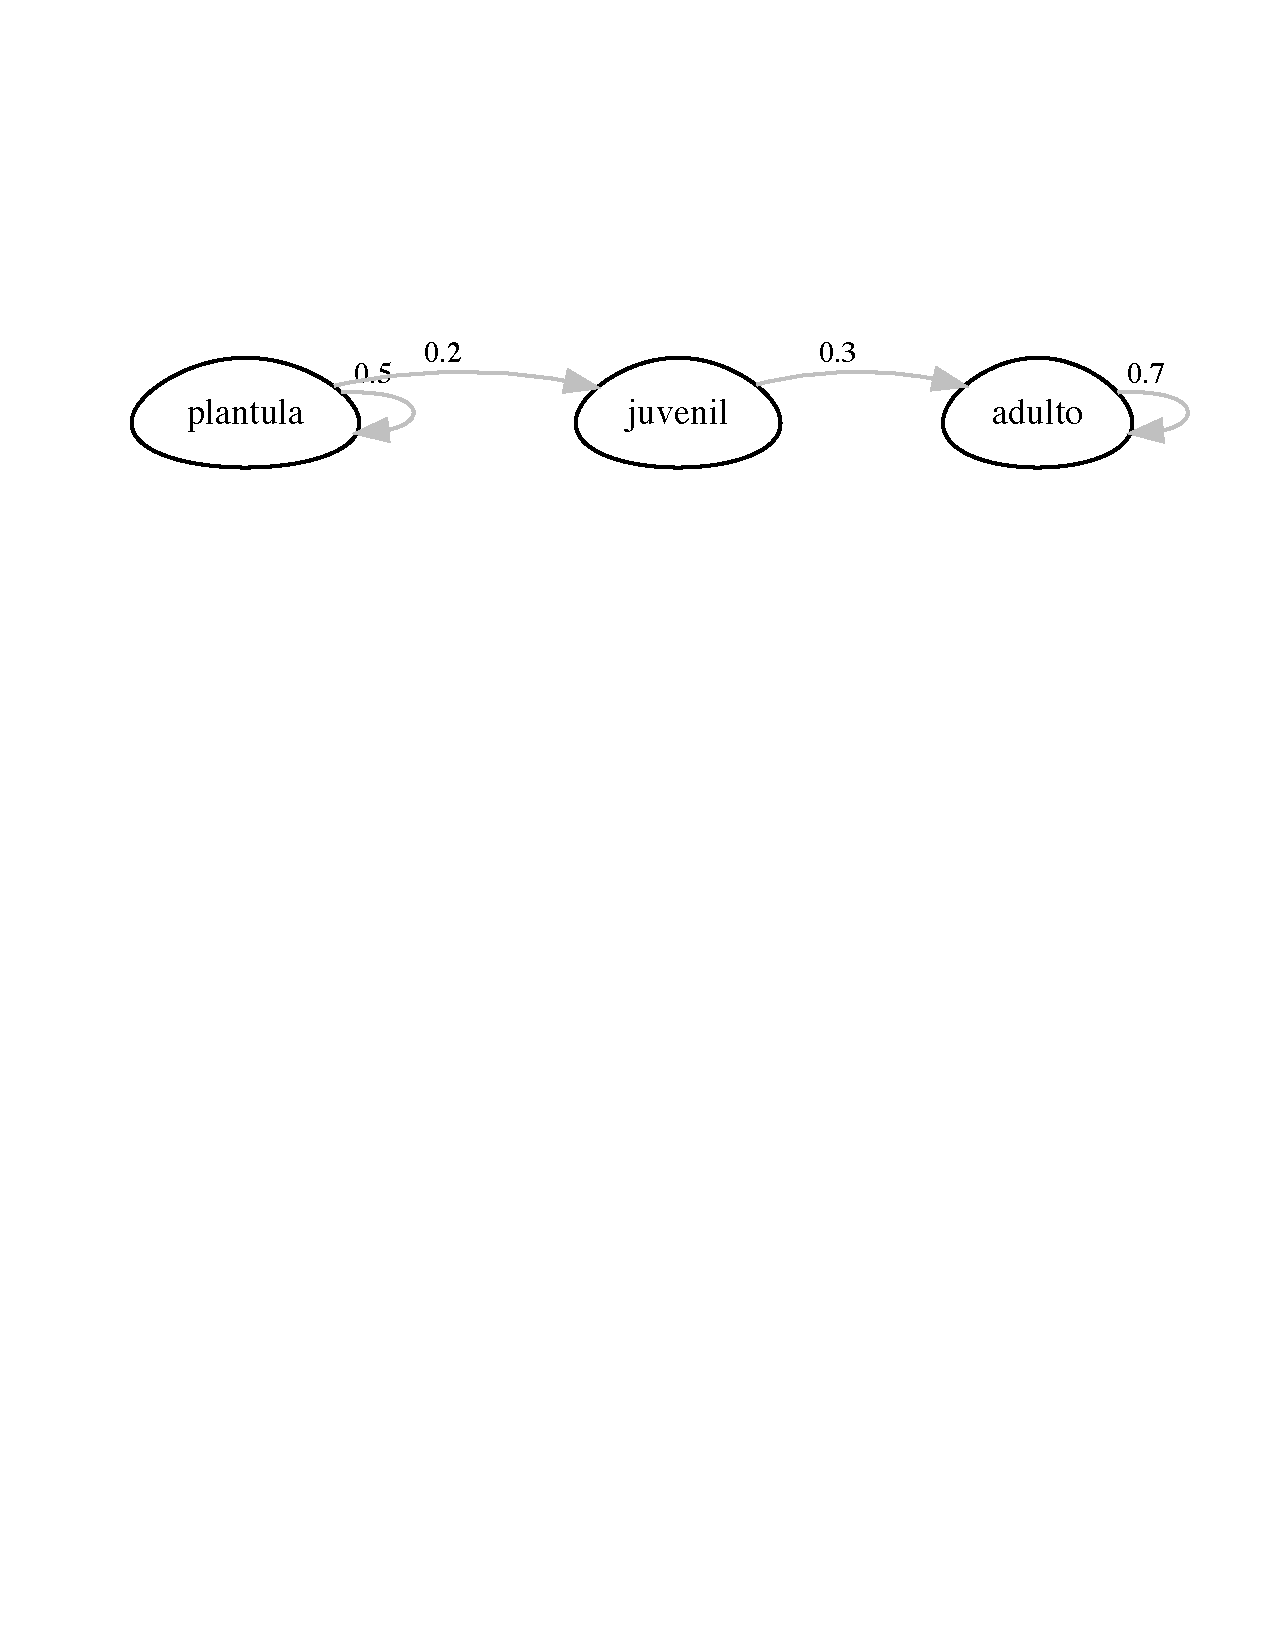
\includegraphics[keepaspectratio]{122-Impacto_de_Datos_sin_Sentido_files/figure-pdf/sin_sentido_15-1.pdf}}

Para evaluar el intervalo ICr del 95\% simultáneamente de las cuatro
transiciones (plántulas a plántulas, plántulas a juvenil, plántulas a
adultos y plántulas a muerte), usamos la \textbf{library(MCMCpack)}, que
es un paquete dedicado a realizar simulaciones de Monte Carlo de Cadenas
Markovianas (\emph{Markov Chain Monte Carlo}). Para lo cual usaremos la
función \texttt{MCmultinomdirichlet}. Tenga en cuenta que la primera
lista son las proporciones que se muestran en la matriz para la etapa de
plántula \texttt{c(.50*n,\ .2*n,\ .0*n,\ .3*n)} multiplicadas por el
tamaño de la muestra \texttt{n\ =\ 25}. La segunda lista son las previas
bayesianas \texttt{c(0.5,\ 0.2,\ 0.0001,\ 0.2999)}; en este caso
asumimos que la suma de las previas es igual a 1. Esto da como resultado
una confianza muy baja en la percepción previa de lo que son las
transiciones --- estamos dando muy poco peso a la percepción previa en
los análisis. Otra opción de previa para la transición es que sean
iguales; podríamos haber usado \texttt{c(1,\ 1,\ .0001,\ 1)}, donde esta
previa sugiere una transición igual para todos los estados menos para la
transición de plántula a adulto. IMPORTANTE: las previas deberían ser
\textbf{biológicamente realistas}, usando lo conocido de la biología de
los organismos que se estudian. Por experiencia y usando la literatura
se puede hacer un estimado de las transiciones y usarlo como previa. El
concepto de lo anterior no se puede explicar completamente aquí;
consulte las siguientes referencias ({Schoot et~al.}, 2021; Tremblay
et~al., 2021).

Los resultados en la figura muestran que hay mucha dispersión alrededor
de la proporción media de las estasis y las transiciones, como se
esperaba debido al pequeño tamaño de la muestra.

\begin{itemize}
\tightlist
\item
  Hacemos una simulación de 100,000.
\item
  Recolectamos los resultados en la variable \textbf{L}.
\item
  Convertimos esta lista en un data frame.
\item
  Reorganizamos el data frame para que sea más fácil de graficar con la
  función \emph{stack}.
\item
  Añadimos una columna con el tamaño de muestra, n=25.
\item
  Cambiamos los nombres de las etapas de la vida para que sean más
  fáciles de leer en la gráfica.
\item
  Graficamos los resultados
\end{itemize}

\begin{Shaded}
\begin{Highlighting}[]
\NormalTok{n }\OtherTok{=} \DecValTok{25}
\NormalTok{L }\OtherTok{=}\NormalTok{ posteriorPRIORL }\OtherTok{\textless{}{-}} \FunctionTok{MCmultinomdirichlet}\NormalTok{(}
  \FunctionTok{c}\NormalTok{(.}\DecValTok{50} \SpecialCharTok{*}\NormalTok{ n, .}\DecValTok{2} \SpecialCharTok{*}\NormalTok{ n, .}\DecValTok{0} \SpecialCharTok{*}\NormalTok{ n, .}\DecValTok{3} \SpecialCharTok{*}\NormalTok{ n),}
  \FunctionTok{c}\NormalTok{(.}\DecValTok{5}\NormalTok{, .}\DecValTok{2}\NormalTok{, }\FloatTok{0.0001}\NormalTok{, .}\DecValTok{3}\NormalTok{),}
  \AttributeTok{mc =} \DecValTok{100000}
\NormalTok{)}
\NormalTok{dfL }\OtherTok{=} \FunctionTok{as.data.frame}\NormalTok{(L)}
\FunctionTok{t}\NormalTok{(}\FunctionTok{summary}\NormalTok{(dfL))}
\end{Highlighting}
\end{Shaded}

\begin{verbatim}
                                                                     
     pi.1 Min.   :0.1274      1st Qu.:0.4330      Median :0.4995     
     pi.2 Min.   :0.01148     1st Qu.:0.14400     Median :0.19218    
     pi.3 Min.   :0.000e+00   1st Qu.:0.000e+00   Median :0.000e+00  
     pi.4 Min.   :0.04759     1st Qu.:0.23665     Median :0.29502    
                                                                     
     pi.1 Mean   :0.4996      3rd Qu.:0.5661      Max.   :0.8834     
     pi.2 Mean   :0.20011     3rd Qu.:0.24852     Max.   :0.66373    
     pi.3 Mean   :5.243e-06   3rd Qu.:0.000e+00   Max.   :9.728e-02  
     pi.4 Mean   :0.30030     3rd Qu.:0.35776     Max.   :0.70621    
\end{verbatim}

\begin{Shaded}
\begin{Highlighting}[]
\CommentTok{\#head(dfL)}
\NormalTok{stack\_dfL }\OtherTok{=} \FunctionTok{stack}\NormalTok{(dfL)}
\NormalTok{comb\_dfbL }\OtherTok{=} \FunctionTok{cbind}\NormalTok{(stack\_dfL, }\AttributeTok{T =} \StringTok{"25"}\NormalTok{)}

\NormalTok{All\_Data3 }\OtherTok{=}\NormalTok{ comb\_dfbL}
\FunctionTok{levels}\NormalTok{(All\_Data3}\SpecialCharTok{$}\NormalTok{ind)[}\FunctionTok{levels}\NormalTok{(All\_Data3}\SpecialCharTok{$}\NormalTok{ind) }\SpecialCharTok{==} \StringTok{"pi.1"}\NormalTok{] }\OtherTok{=} \StringTok{"Plántulas"}
\FunctionTok{levels}\NormalTok{(All\_Data3}\SpecialCharTok{$}\NormalTok{ind)[}\FunctionTok{levels}\NormalTok{(All\_Data3}\SpecialCharTok{$}\NormalTok{ind) }\SpecialCharTok{==} \StringTok{"pi.2"}\NormalTok{] }\OtherTok{=} \StringTok{"Juvenil"}
\FunctionTok{levels}\NormalTok{(All\_Data3}\SpecialCharTok{$}\NormalTok{ind)[}\FunctionTok{levels}\NormalTok{(All\_Data3}\SpecialCharTok{$}\NormalTok{ind) }\SpecialCharTok{==} \StringTok{"pi.3"}\NormalTok{] }\OtherTok{=} \StringTok{"Adulto"}
\FunctionTok{levels}\NormalTok{(All\_Data3}\SpecialCharTok{$}\NormalTok{ind)[}\FunctionTok{levels}\NormalTok{(All\_Data3}\SpecialCharTok{$}\NormalTok{ind) }\SpecialCharTok{==} \StringTok{"pi.4"}\NormalTok{] }\OtherTok{=} \StringTok{"Muerto"}
\end{Highlighting}
\end{Shaded}

\begin{itemize}
\tightlist
\item
  Graficamos los resultados
\end{itemize}

\begin{Shaded}
\begin{Highlighting}[]
\FunctionTok{ggplot}\NormalTok{(}\AttributeTok{data =}\NormalTok{ All\_Data3, }\FunctionTok{aes}\NormalTok{(}\AttributeTok{x =}\NormalTok{ values, }\AttributeTok{fill =}\NormalTok{ ind)) }\SpecialCharTok{+}
  \FunctionTok{geom\_density}\NormalTok{(}\AttributeTok{alpha =}\NormalTok{ .}\DecValTok{5}\NormalTok{) }\SpecialCharTok{+}
  \FunctionTok{scale\_y\_continuous}\NormalTok{(}\AttributeTok{limit =} \FunctionTok{c}\NormalTok{(}\DecValTok{0}\NormalTok{, }\FloatTok{5.5}\NormalTok{)) }\SpecialCharTok{+}
  \FunctionTok{scale\_colour\_hue}\NormalTok{(}\AttributeTok{l =} \DecValTok{60}\NormalTok{) }\SpecialCharTok{+}
  \FunctionTok{facet\_grid}\NormalTok{(}\SpecialCharTok{\textasciitilde{}}\NormalTok{ind) }\SpecialCharTok{+}
  \FunctionTok{ylab}\NormalTok{(}
    \StringTok{"La distribución de las proporciones }\SpecialCharTok{\textbackslash{}n}\StringTok{ de plántulas que crecen a la siguiente etapa"}
\NormalTok{  ) }\SpecialCharTok{+}
  \FunctionTok{xlab}\NormalTok{(}\StringTok{"Proporciones"}\NormalTok{) }\SpecialCharTok{+}
  \FunctionTok{labs}\NormalTok{(}\AttributeTok{fill =} \StringTok{"Etapa de vida"}\NormalTok{)}\SpecialCharTok{+}
  \FunctionTok{rlt\_style\_fill}\NormalTok{()}
\end{Highlighting}
\end{Shaded}

\pandocbounded{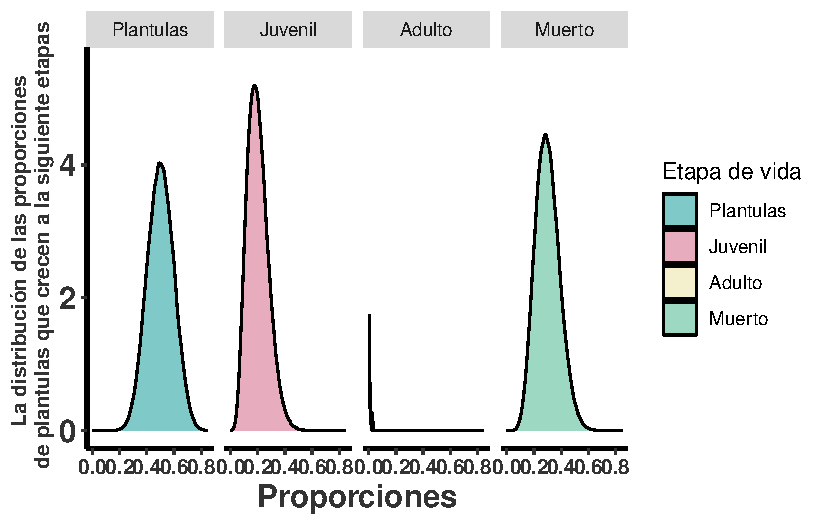
\includegraphics[keepaspectratio]{122-Impacto_de_Datos_sin_Sentido_files/figure-pdf/sin_sentido_17-1.pdf}}

Ahora calculemos el ICr del 95\% de las transiciones

Ahora que los datos están organizados en un \emph{data frame} es fácil
extraer los valores de las transiciones y calcular los intervalos de
credibilidad del 95\% de las transiciones, estasis y supervivencia. Para
ello usamos la función \texttt{ddply} del paquete \texttt{plyr} para
resumir los datos por la columna \texttt{ind} (etapa de vida) y calcular
el promedio, desviación estándar, mediana, cuantil 5\% y cuantil 95\% de
los valores de cada etapa.

\begin{itemize}
\tightlist
\item
  Intervalos de credibilidad de transiciones, estasis y supervivencia
  basados en simulación y distribución de Dirichlet.
\end{itemize}

Aspectos importantes a tener en cuenta.

\begin{itemize}
\tightlist
\item
  los ICr del 95\% están acotados entre 0 y 1. Los valores por debajo de
  cero o por encima de uno en los parámetros no tendrían sentido.
\item
  la suma de los promedios es igual a 1.
\item
  la forma de la distribución no se distribuye normalmente, ver figura
  anterior. La forma de la distribución se llama distribución beta.
\end{itemize}

\begin{Shaded}
\begin{Highlighting}[]
\NormalTok{Transiciones }\OtherTok{=} \FunctionTok{ddply}\NormalTok{(}
\NormalTok{  All\_Data3,}
  \FunctionTok{c}\NormalTok{(}\StringTok{"ind"}\NormalTok{),}
\NormalTok{  summarise,}
  \AttributeTok{mean =} \FunctionTok{round}\NormalTok{(}\FunctionTok{mean}\NormalTok{(values), }\DecValTok{4}\NormalTok{),}
  \AttributeTok{sd =} \FunctionTok{round}\NormalTok{(}\FunctionTok{sd}\NormalTok{(values), }\DecValTok{5}\NormalTok{),}
  \AttributeTok{median =} \FunctionTok{round}\NormalTok{(}\FunctionTok{median}\NormalTok{(values), }\DecValTok{4}\NormalTok{),}
  \CommentTok{\#sem = round(sd(values)/sqrt(length(values)),6), \# para calcular el error estándar de la media}
  \AttributeTok{ICr5 =} \FunctionTok{round}\NormalTok{(}\FunctionTok{quantile}\NormalTok{(values, }\AttributeTok{probs =} \FunctionTok{c}\NormalTok{(}\FloatTok{0.05}\NormalTok{)), }\DecValTok{4}\NormalTok{), }\CommentTok{\# el cuantil 5}
  \AttributeTok{ICr95 =} \FunctionTok{round}\NormalTok{(}\FunctionTok{quantile}\NormalTok{(values, }\AttributeTok{probs =} \FunctionTok{c}\NormalTok{(}\FloatTok{0.95}\NormalTok{)), }\DecValTok{4}\NormalTok{), }\CommentTok{\# el cuantil 95}
  \AttributeTok{min =} \FunctionTok{min}\NormalTok{(values),}
  \AttributeTok{max =} \FunctionTok{max}\NormalTok{(values)}
\NormalTok{)}

\NormalTok{Transiciones}
\end{Highlighting}
\end{Shaded}

\begin{verbatim}
        ind   mean      sd median   ICr5  ICr95        min        max
1 Plántulas 0.4996 0.09596 0.4995 0.3417 0.6574 0.12741535 0.88335868
2   Juvenil 0.2001 0.07683 0.1922 0.0875 0.3384 0.01148408 0.66373403
3    Adulto 0.0000 0.00045 0.0000 0.0000 0.0000 0.00000000 0.09727822
4    Muerto 0.3003 0.08831 0.2950 0.1645 0.4546 0.04758920 0.70620551
\end{verbatim}

Para visualizar los intervalos de credibilidad de las otras transiciones
basta con cambiar las variables de la función \texttt{L} y \texttt{n}.
En este caso, cambiamos el tamaño de la muestra correspondiente a esta
etapa.

\begin{center}\rule{0.5\linewidth}{0.5pt}\end{center}

\subsection{Tamaño de muestra y estimaciones de intervalos de confianza
con
n2=250}\label{tamauxf1o-de-muestra-y-estimaciones-de-intervalos-de-confianza-con-n2250}

Para comparar con el ejemplo anterior asumimos que en lugar de tener
solamente 25 plántulas teníamos 250 para las estimaciones.

Note que con los mismos estimados puntuales pero con un tamaño de
muestra mayor la mediana sigue en el mismo lugar (casi) pero los ICr
cambian mucho y son más reducidos los anchos de la dispersión, ya que
con más datos en el muestreo existe más confianza resultado de una
reducción en el ICr. Este análisis es primordial para entender la
confianza que uno debería tener sobre los estimados de los parámetros de
la matriz. Si se observa un ICr muy grande, se recomendaría modificar la
recolección de datos en el campo para aumentar el tamaño de muestra de
esa etapa específica.

\begin{Shaded}
\begin{Highlighting}[]
\NormalTok{n2 }\OtherTok{=} \DecValTok{250}
\NormalTok{L }\OtherTok{=}\NormalTok{ posteriorPRIORL }\OtherTok{\textless{}{-}} \FunctionTok{MCmultinomdirichlet}\NormalTok{(}
  \FunctionTok{c}\NormalTok{(.}\DecValTok{50} \SpecialCharTok{*}\NormalTok{ n2, .}\DecValTok{2} \SpecialCharTok{*}\NormalTok{ n2, .}\DecValTok{0} \SpecialCharTok{*}\NormalTok{ n2, .}\DecValTok{3} \SpecialCharTok{*}\NormalTok{ n2),}
  \FunctionTok{c}\NormalTok{(.}\DecValTok{5}\NormalTok{, .}\DecValTok{2}\NormalTok{, }\FloatTok{0.0001}\NormalTok{, .}\DecValTok{3}\NormalTok{),}
  \AttributeTok{mc =} \DecValTok{100000}
\NormalTok{)}
\NormalTok{dfL }\OtherTok{=} \FunctionTok{as.data.frame}\NormalTok{(L)}
\FunctionTok{t}\NormalTok{(}\FunctionTok{summary}\NormalTok{(dfL))}
\end{Highlighting}
\end{Shaded}

\begin{verbatim}
                                                                     
     pi.1 Min.   :0.3624      1st Qu.:0.4788      Median :0.5000     
     pi.2 Min.   :0.1024      1st Qu.:0.1824      Median :0.1992     
     pi.3 Min.   :0.000e+00   1st Qu.:0.000e+00   Median :0.000e+00  
     pi.4 Min.   :0.1873      1st Qu.:0.2802      Median :0.2993     
                                                                     
     pi.1 Mean   :0.5001      3rd Qu.:0.5215      Max.   :0.6234     
     pi.2 Mean   :0.1999      3rd Qu.:0.2164      Max.   :0.3309     
     pi.3 Mean   :2.211e-07   3rd Qu.:0.000e+00   Max.   :2.944e-03  
     pi.4 Mean   :0.3000      3rd Qu.:0.3191      Max.   :0.4341     
\end{verbatim}

\begin{Shaded}
\begin{Highlighting}[]
\CommentTok{\#head(dfL)}
\NormalTok{stack\_dfL }\OtherTok{=} \FunctionTok{stack}\NormalTok{(dfL)}
\NormalTok{comb\_dfbL }\OtherTok{=} \FunctionTok{cbind}\NormalTok{(stack\_dfL, }\AttributeTok{T =} \StringTok{"25"}\NormalTok{)}

\NormalTok{All\_Data4 }\OtherTok{=}\NormalTok{ comb\_dfbL}
\FunctionTok{levels}\NormalTok{(All\_Data4}\SpecialCharTok{$}\NormalTok{ind)[}\FunctionTok{levels}\NormalTok{(All\_Data4}\SpecialCharTok{$}\NormalTok{ind) }\SpecialCharTok{==} \StringTok{"pi.1"}\NormalTok{] }\OtherTok{=} \StringTok{"Plántulas"}
\FunctionTok{levels}\NormalTok{(All\_Data4}\SpecialCharTok{$}\NormalTok{ind)[}\FunctionTok{levels}\NormalTok{(All\_Data4}\SpecialCharTok{$}\NormalTok{ind) }\SpecialCharTok{==} \StringTok{"pi.2"}\NormalTok{] }\OtherTok{=} \StringTok{"Juvenil"}
\FunctionTok{levels}\NormalTok{(All\_Data4}\SpecialCharTok{$}\NormalTok{ind)[}\FunctionTok{levels}\NormalTok{(All\_Data4}\SpecialCharTok{$}\NormalTok{ind) }\SpecialCharTok{==} \StringTok{"pi.3"}\NormalTok{] }\OtherTok{=} \StringTok{"Adulto"}
\FunctionTok{levels}\NormalTok{(All\_Data4}\SpecialCharTok{$}\NormalTok{ind)[}\FunctionTok{levels}\NormalTok{(All\_Data4}\SpecialCharTok{$}\NormalTok{ind) }\SpecialCharTok{==} \StringTok{"pi.4"}\NormalTok{] }\OtherTok{=} \StringTok{"Muerto"}

\FunctionTok{ggplot}\NormalTok{(}\AttributeTok{data =}\NormalTok{ All\_Data4, }\FunctionTok{aes}\NormalTok{(}\AttributeTok{x =}\NormalTok{ values, }\AttributeTok{fill =}\NormalTok{ ind)) }\SpecialCharTok{+}
  \FunctionTok{geom\_density}\NormalTok{(}\FunctionTok{aes}\NormalTok{(}\AttributeTok{alpha =}\NormalTok{ .}\DecValTok{5}\NormalTok{)) }\SpecialCharTok{+}
  \FunctionTok{scale\_y\_continuous}\NormalTok{(}\AttributeTok{limit =} \FunctionTok{c}\NormalTok{(}\DecValTok{0}\NormalTok{, }\DecValTok{18}\NormalTok{)) }\SpecialCharTok{+}
  \FunctionTok{scale\_colour\_hue}\NormalTok{(}\AttributeTok{l =} \DecValTok{60}\NormalTok{) }\SpecialCharTok{+}
  \FunctionTok{facet\_grid}\NormalTok{(}\SpecialCharTok{\textasciitilde{}}\NormalTok{ind) }\SpecialCharTok{+}
  \FunctionTok{labs}\NormalTok{(}\AttributeTok{fill =} \StringTok{"Etapa de vida"}\NormalTok{)}\SpecialCharTok{+}
  \FunctionTok{rlt\_style\_fill}\NormalTok{()}
\end{Highlighting}
\end{Shaded}

\pandocbounded{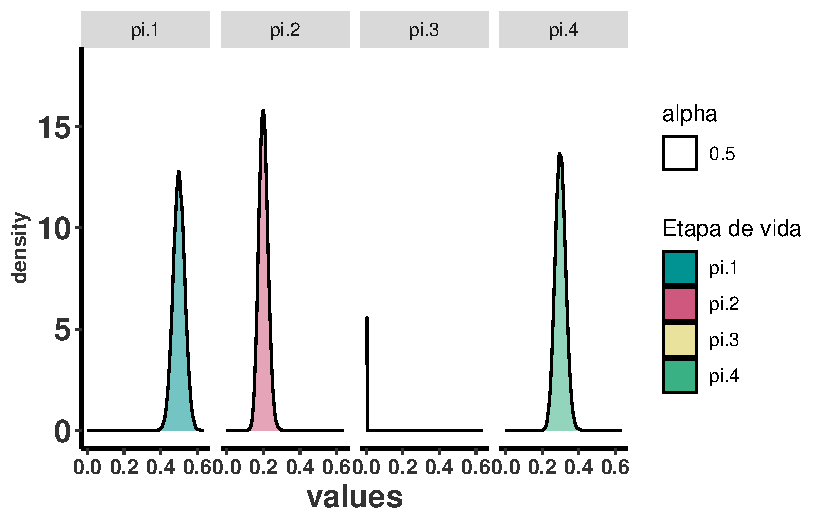
\includegraphics[keepaspectratio]{122-Impacto_de_Datos_sin_Sentido_files/figure-pdf/sin_sentido_19-1.pdf}}

\subsection{Los estimados de intervalo de credibilidad con un tamaño de
muestra de
n=250}\label{los-estimados-de-intervalo-de-credibilidad-con-un-tamauxf1o-de-muestra-de-n250}

Note que ahora los intervalos de credibilidad son más estrechos y no son
negativos ni mayores de uno.

\begin{Shaded}
\begin{Highlighting}[]
\NormalTok{Transiciones }\OtherTok{=} \FunctionTok{ddply}\NormalTok{(}
\NormalTok{  All\_Data4,}
  \FunctionTok{c}\NormalTok{(}\StringTok{"ind"}\NormalTok{),}
\NormalTok{  summarise,}
  \AttributeTok{mean =} \FunctionTok{round}\NormalTok{(}\FunctionTok{mean}\NormalTok{(values), }\DecValTok{3}\NormalTok{),}
  \AttributeTok{sd =} \FunctionTok{round}\NormalTok{(}\FunctionTok{sd}\NormalTok{(values), }\DecValTok{4}\NormalTok{),}
  \AttributeTok{median =} \FunctionTok{median}\NormalTok{(values),}
  \CommentTok{\#sem = round(sd(values)/sqrt(length(values)),6),}
  \AttributeTok{CI5 =} \FunctionTok{quantile}\NormalTok{(values, }\AttributeTok{probs =} \FunctionTok{c}\NormalTok{(}\FloatTok{0.05}\NormalTok{)),}
  \AttributeTok{CI95 =} \FunctionTok{round}\NormalTok{(}\FunctionTok{quantile}\NormalTok{(values, }\AttributeTok{probs =} \FunctionTok{c}\NormalTok{(}\FloatTok{0.95}\NormalTok{)), }\DecValTok{4}\NormalTok{),}
  \AttributeTok{min =} \FunctionTok{min}\NormalTok{(values),}
  \AttributeTok{max =} \FunctionTok{max}\NormalTok{(values)}
\NormalTok{)}

\NormalTok{Transiciones}
\end{Highlighting}
\end{Shaded}

\begin{verbatim}
        ind mean     sd    median       CI5   CI95       min         max
1 Plántulas  0.5 0.0315 0.5000285 0.4484404 0.5518 0.3624084 0.623441934
2   Juvenil  0.2 0.0253 0.1991515 0.1597542 0.2431 0.1024335 0.330899715
3    Adulto  0.0 0.0000 0.0000000 0.0000000 0.0000 0.0000000 0.002943776
4    Muerto  0.3 0.0287 0.2993493 0.2536744 0.3482 0.1873420 0.434077870
\end{verbatim}

\bookmarksetup{startatroot}

\chapter{Conclusión}\label{conclusiuxf3n}

\emph{Por: Raymond L. Tremblay, Demetria Mondragón y Aucencia
Emeterio-Lara}

La gama de acercamientos desarrollada en este libro permite ser
utilizado para evaluar una gran diversidad de hipótesis y temas. Pero,
sin duda lo más importante no son las técnicas matemáticas sino las
preguntas que se pueden responder con la información presentada. Las
hipótesis que se presentan desde el punto de vista de conservación,
ecología, historia de vida y evolución, son solo ejemplos de preguntas
que pueden ser respondidas con los modelos de dinámica poblacional. Gran
parte del libro está dedicado a resaltar los métodos cuantitativos y sus
limitaciones, reconociendo que para realizar análisis de dinámica
poblacional hay que entender todos los pasos y tener presente que, en
cualquiera de estos casos, existen errores cuantitativos y de
interpretación, que pueden invalidar el trabajo final. Los autores de
este libro reconocen que el estudio de la dinámica poblacional es
holístico y permite evaluar historias de vida complejas.

Más allá del catálogo de técnicas, este libro busca cumplir tres
funciones que rara vez aparecen reunidas en un mismo texto sobre
dinámica poblacional. Primero, \textbf{traducir al español} un conjunto
de métodos que, en su mayoría, sólo están documentados en inglés.
Segundo, \textbf{anclar cada método en un ejemplo de orquídeas} ---un
grupo cuya historia de vida (semillas microscópicas, dependencia de
micorrizas, longevidad alta, eventos reproductivos raros) pone a prueba
los supuestos clásicos del modelado matricial y obliga a tomar
decisiones explícitas. Tercero, \textbf{dar herramientas para
diagnosticar la calidad} de un análisis matricial poblacional, no sólo
para construirlo: los capítulos sobre métodos bayesianos, sobre el
protocolo de reporte estandarizado y sobre los impactos de datos sin
sentido biológico, en conjunto, ofrecen una vía para que el lector pueda
evaluar críticamente su propio trabajo y la literatura existente.

En esta sección presentamos primero los aportes metodológicos del libro
y, a continuación, algunas preguntas principales que pueden ser
abordadas en el futuro.

\section{Aportes metodológicos del
libro}\label{aportes-metodoluxf3gicos-del-libro}

Conviene resumir los componentes más singulares del libro y la pregunta
a la que cada uno responde:

\begin{itemize}
\item
  \textbf{Métodos bayesianos para transiciones raras.} Cuando una
  transición biológicamente posible nunca se observó en el muestreo
  ---por ejemplo, la mortalidad de un adulto longevo o la germinación de
  una semilla microscópica---, el estimador frecuentista es exactamente
  cero o uno, lo que produce matrices reducibles, supervivencias
  perfectas o intervalos de confianza fuera de {[}0, 1{]}. Las
  distribuciones Beta y Dirichlet, combinadas con un previo informado
  por la literatura, permiten estimar valores que respetan los límites
  biológicos y propagar la incertidumbre al cálculo de \(\lambda\). Es
  probablemente la herramienta más útil del libro para especies raras o
  en peligro (Tremblay et~al., 2021).
\item
  \textbf{Descomposición U / F / C.} Separar la matriz A en sus
  componentes de supervivencia/crecimiento (U), reproducción sexual (F)
  y reproducción clonal (C) no es sólo cosmético: muchas métricas
  demográficas derivadas ---esperanza de vida, tiempo generacional, edad
  a primera reproducción, varianza en la reproducción de por vida---
  sólo pueden calcularse desde las submatrices, no desde A. Es la
  descomposición que requieren los paquetes \texttt{Rage} y los análisis
  basados en cadenas de Markov absorbentes ({Jones et~al.}, 2022).
\item
  \textbf{Análisis LTRE entre grupos contrastantes.} La técnica de
  Caswell de descomponer una diferencia observada en \(\lambda\) en
  contribuciones de las distintas tasas vitales subyacentes es
  especialmente potente cuando se compara la misma especie en sustratos
  o ambientes diferentes ---como el ejemplo de \emph{Lepanthes} sobre
  distintas especies de \emph{Quercus} (Ramı́rez Martı́nez, 2021). La
  magnitud absoluta de \(\lambda\) esconde quién está pagando el costo
  demográfico; el LTRE lo revela.
\item
  \textbf{Funciones de transferencia para elasticidad no lineal.} Las
  elasticidades clásicas son válidas sólo para perturbaciones
  infinitesimales. Cuando la perturbación es grande ---una intervención
  de manejo, una caída drástica de la fecundidad por sequía, una cosecha
  intensa---, el comportamiento de \(\lambda\) se vuelve no lineal, y
  las funciones de transferencia (Stott, Hodgson \& Townley, 2012a)
  capturan esa no linealidad de manera explícita.
\item
  \textbf{Dinámica transitoria.} Buena parte de la teoría matricial se
  centra en el comportamiento asintótico (\(\lambda\), distribución
  estable, valor reproductivo), pero las poblaciones reales ---en
  especial las pequeñas, recientemente perturbadas, o restauradas---
  viven en el régimen transitorio durante décadas. Las métricas de
  (Stott, Townley \& Hodgson, 2011) (amplificación, atenuación,
  reactividad) cuantifican qué tan lejos puede alejarse la población del
  comportamiento asintótico antes de converger a él.
\item
  \textbf{Simulaciones estocásticas.} La aproximación de Tuljapurkar y
  la simulación de Cohen ofrecen dos rutas complementarias para
  incorporar la variabilidad ambiental al cálculo de la tasa de
  crecimiento. La simulación, aunque más costosa computacionalmente,
  admite distribuciones arbitrarias de matrices y es indispensable para
  evaluar el riesgo de cuasi-extinción.
\item
  \textbf{Acceso programático a COMPADRE y demografía con
  \texttt{Rage}.} El acceso a más de 8 000 matrices revisadas por pares
  cambia la escala de las preguntas posibles: en lugar de un solo
  estudio de caso, hoy son factibles comparaciones filogenéticas,
  geográficas o por hábitos de vida sobre cientos de especies.
\item
  \textbf{Protocolo estandarizado para reportar MPP.} La traducción al
  español del protocolo de Gascoigne et al. ({Gascoigne et~al.}, 2023)
  busca que los datos demográficos producidos en países de habla hispana
  puedan ser fácilmente integrados a las bases de datos globales y
  replicados por otros investigadores.
\item
  \textbf{Diagnóstico de datos sin sentido biológico.} Es uno de los
  componentes más originales del libro y, en cierto sentido, el más
  importante: incluso un análisis matemáticamente impecable produce
  resultados engañosos si los datos no respetan la biología del
  organismo. El capítulo correspondiente agrupa los errores más
  frecuentes y, para cada uno, ofrece código R para detectarlos y un
  camino para corregirlos.
\item
  \textbf{Historia y figuras fundadoras.} Documentar las raíces del
  estudio demográfico de orquídeas ---en particular el papel de Carl
  Olaf Tamm--- evita que las nuevas generaciones repitan errores ya
  identificados hace décadas y permite reconocer a quienes establecieron
  el campo.
\end{itemize}

\section{Preguntas ecológicas}\label{preguntas-ecoluxf3gicas}

\begin{itemize}
\item
  Aunque la mayoría de las especies de orquídeas tienen solamente un
  polinizador, para aquellas que tienen múltiples especies de
  polinizadores no está claro si esto afecta la dinámica de sus
  poblaciones (Tremblay, 1992; Ackerman et~al., 2025). En otras
  palabras: ¿las especies con múltiples polinizadores tienen una mayor
  consistencia poblacional al compararlas con las especies con un solo
  polinizador? Y de ser el caso, ¿cuáles son los factores que lo están
  promoviendo? Por ejemplo, cuando uno evalúa la diversidad de polinios
  sobre los polinizadores, esa diversidad pudiese tener repercusiones en
  la producción de frutos y la calidad de las semillas, y esto a su vez
  pudiera verse reflejado en las tasas de fecundidad y sobrevivencia de
  las plántulas, lo que sugiere un efecto sobre la dinámica de las
  poblaciones. Desafortunadamente, se conoce muy poco sobre el efecto de
  la diversidad de padres sobre la calidad de las semillas (Tremblay,
  1994; Light \& MacConaill, 1998).
\item
  Típicamente los modelos están basados en las cifras de reclutamiento
  que se observan en el laboratorio (\emph{in vitro}), lo cual es una
  subestimación de la mortandad en el campo y una sobreestimación del
  potencial de reclutamiento, ya que a dicho valor se le debieran
  incorporar eventos estocásticos como la proporción de semillas que
  llegan a un micronicho apropiado para la germinación, la proporción de
  semillas que germinan bajo las condiciones microambientales en las que
  se desarrollan, las pérdidas por herbivoría o por desecación, etc. No
  está claro si esta subestimación es relevante en la dinámica de las
  especies en ambientes naturales. La evaluación de la germinación de
  semillas en el campo, dado su pequeño tamaño y la dificultad de
  detectarlas, así como los protocolos asociados, es un reto que
  necesita ser explorado con profundidad. Habrá necesidad de evaluar
  técnicas de germinación \emph{in vivo} que permitan el monitoreo del
  reclutamiento a mediano plazo para tener cifras más exactas del número
  que integra la nueva generación de individuos (plántulas). En general,
  se conoce muy poco sobre la proporción de las semillas producidas y
  los valores de germinación en el campo (Ackerman, Sabat \& Zimmerman,
  1996; Ehrlén \& Eriksson, 2000; Batty et~al., 2001; Wilcock \&
  Neiland, 2002).
\item
  El efecto de las variables abióticas sobre la historia de vida de las
  plantas comienza a ser investigado (Morris et~al., 2020), y su efecto
  sobre orquídeas es un tema que merece atención. Por ejemplo, ¿cuál es
  el efecto de los patrones de variación abiótica sobre la persistencia
  de las poblaciones y su dinámica a largo plazo?
\item
  Los efectos bióticos tales como la herbivoría, las interacciones con
  polinizadores, la interacción con árboles forófitos (en el caso de
  orquídeas epífitas), la diversidad de micorrizas en la raíz de las
  orquídeas, etc., pudieran influir sobre los parámetros de las matrices
  de proyección poblacional (MPP), por lo que se necesita explorar a
  mayor profundidad dichos efectos.
\item
  Aunque los ecólogos que trabajan con orquídeas reconocen que muchas
  especies se multiplican clonalmente, aparte de los trabajos de
  \emph{Cypripedium} (Garcı́a González, Goñi \& Guzmán, 2010) no es
  evidente su impacto sobre la persistencia y dinámica de estas
  poblaciones. Muchas otras especies de orquídeas tienen una historia de
  vida que incluye clonaje, tales como \emph{Epidendrum} y
  \emph{Artorima}, pero no se ha evaluado su impacto sobre la dinámica
  poblacional.
\item
  Los trabajos de orquídeas epífitas han determinado la dinámica
  poblacional con información de la orquídea, desligada del forófito;
  sin embargo, considerando que no son plantas con crecimiento
  independiente del sustrato, ¿de qué manera se puede incluir el efecto
  o importancia del forófito en los modelos demográficos? El único
  trabajo que evaluó el efecto del forófito sobre la dinámica
  poblacional de una orquídea epífita fue el de \emph{Oncidium
  brachyandrum} (Ramı́rez Martı́nez, 2021), en su tesis doctoral. El
  efecto de los diferentes hospederos de \emph{Quercus} es dramático;
  vea el capítulo de LTRE/ERTV.
\item
  ¿Cuál es la relación de la diversidad micorrízica, el ciclo de vida y
  la adecuación evolutiva? En otras palabras, ¿individuos con mayor
  diversidad micorrízica tienen una mayor adecuación evolutiva que
  individuos con menos diversidad de hongos micorrízicos? O ¿los que
  tienen un simbionte específico tienen una mayor adecuación evolutiva,
  influenciando la edad a la primera reproducción o el esfuerzo
  reproductivo?
\item
  ¿Cómo afectan los eventos climáticos extremos ---huracanes, sequías
  prolongadas, heladas atípicas--- las tasas vitales de las orquídeas?
  El análisis LTRE permite atribuir el cambio observado en \(\lambda\)
  después de un evento a las tasas vitales específicas afectadas, y los
  métodos estocásticos permiten incorporar la frecuencia esperada de
  tales eventos al cálculo de la tasa de crecimiento promedio en
  escenarios climáticos futuros.
\item
  ¿Las poblaciones recién colonizadas o restauradas se comportan como
  predicen sus matrices asintóticas? Las métricas de dinámica
  transitoria están especialmente diseñadas para responder esta
  pregunta: una población lejos de su distribución estable de etapas
  puede crecer o decrecer durante décadas a tasas muy distintas de
  \(\lambda\), y la magnitud de ese desfase se cuantifica con la
  reactividad y la amplificación.
\item
  ¿Cómo cambia la dinámica poblacional a lo largo de un gradiente
  altitudinal o latitudinal? La combinación de COMPADRE con métricas
  demográficas derivadas de \texttt{Rage} permite hoy hacer este tipo de
  comparaciones a escala continental para los grupos taxonómicos
  suficientemente representados en la base.
\end{itemize}

\section{Preguntas de conservación}\label{preguntas-de-conservaciuxf3n}

Las técnicas presentadas en este libro son particularmente potentes para
responder preguntas de conservación, dado que la mayoría de las
orquídeas tropicales están listadas o son candidatas a estarlo en alguna
categoría de amenaza:

\begin{itemize}
\item
  La gran mayoría de las orquídeas evaluadas por la UICN están
  clasificadas como \emph{Datos Insuficientes}. Las matrices de tipo MPP
  combinadas con simulación estocástica permiten estimar la
  \textbf{probabilidad de cuasi-extinción} y los \textbf{tiempos
  esperados} para alcanzar tamaños críticos, complementando los
  criterios cualitativos de la UICN con indicadores cuantitativos
  defendibles.
\item
  ¿Cómo se debe priorizar la inversión limitada en conservación entre
  etapas del ciclo de vida? La elasticidad y, cuando las perturbaciones
  son grandes, las funciones de transferencia, identifican qué
  transición o tasa vital tendría el mayor efecto sobre \(\lambda\) si
  se interviniera ---por ejemplo, mediante reforzamiento de plántulas,
  protección de adultos reproductivos o introducción de polinizadores.
\item
  ¿Es viable la cosecha sostenible de una orquídea silvestre? El ejemplo
  de \emph{Euchile karwinskii} (Elliott, 2014) muestra cómo el LTRE
  puede separar el efecto directo de la cosecha sobre la supervivencia
  adulta del efecto indirecto sobre la fecundidad. La pregunta general
  ---¿cuántos individuos pueden extraerse antes de que \(\lambda\) caiga
  por debajo de 1?--- es directamente abordable con los métodos del
  capítulo de funciones de transferencia.
\item
  Las \textbf{translocaciones y reintroducciones} generan poblaciones
  con distribuciones de etapas muy alejadas de la estable. Las métricas
  transitorias permiten predecir si y cuándo la población recuperará un
  comportamiento asintótico, y por cuánto tiempo se mantendrá vulnerable
  después del evento de translocación.
\item
  ¿Cómo afectan los disturbios antropogénicos crónicos ---fragmentación
  de bosque, pérdida de polinizadores, calentamiento global--- la
  viabilidad de las poblaciones? La integración de modelos demográficos
  estructurados con escenarios climáticos (Jenouvrier et~al., 2022) es
  un terreno fértil aún poco explorado en orquídeas.
\item
  En especies con bancos de semillas potenciales o con etapas de
  latencia (como muchas orquídeas terrestres templadas), ¿cuál es la
  contribución del banco de semillas a la persistencia poblacional? Esta
  pregunta exige los métodos bayesianos del capítulo correspondiente,
  dado que la transición desde el banco de semillas rara vez se observa
  directamente y debe inferirse con un previo biológicamente informado.
\item
  ¿Las orquídeas mantenidas \emph{ex situ} (jardines botánicos,
  propagación \emph{in vitro}) presentan una dinámica poblacional
  comparable a la de las poblaciones silvestres? El protocolo del
  capítulo 121 advierte explícitamente que las poblaciones cautivas
  pueden no reflejar las condiciones naturales, y los MPP permiten
  cuantificar el sesgo cuando se cuenta con datos de ambos contextos.
\end{itemize}

\section{Preguntas de historia de
vida}\label{preguntas-de-historia-de-vida}

\begin{itemize}
\item
  ¿Cuáles son las diferencias y similitudes en la historia de vida de
  las orquídeas cuando se comparan epífitas, terrestres, litófitas,
  templadas y tropicales?
\item
  Aunque hay poca diversidad de epífitas en áreas templadas, no están
  ausentes; por ejemplo, \emph{Sarcochilus australis} es una epífita que
  se encuentra en Australia y Tasmania (Tremblay, 2006). En general, las
  orquídeas epífitas tienen una historia de vida diferente a las
  terrestres, pero no se ha evaluado si estas diferencias son relevantes
  para la dinámica poblacional cuando uno considera el ambiente templado
  versus tropical.
\item
  La historia de vida de las especies terrestres en áreas templadas ha
  sido bastante estudiada, pero en ambientes tropicales los estudios son
  escasos. Los que hemos encontrado son solamente los de
  \emph{Oeceoclades maculata} (Riverón-Giró et~al., 2019), \emph{Phaius
  australis} (Simmons, 2016) y \emph{Spathoglottis plicata} (Falcón,
  Ackerman \& Tremblay, 2017). Dado que el ambiente tropical es menos
  variable en temperatura, ¿qué efecto, si alguno, tiene sobre la
  historia de vida de las orquídeas terrestres tropicales comparadas con
  las especies templadas?
\item
  ¿Cómo se comparan los \textbf{tiempos generacionales} y la
  \textbf{edad a primera reproducción} de las orquídeas con los de otras
  familias de plantas? Las funciones \texttt{gen\_time()} y
  \texttt{mature\_age()} de \texttt{Rage} permiten calcularlos
  directamente desde las matrices U y F, abriendo análisis comparativos
  a gran escala con la información ya disponible en COMPADRE.
\item
  La \textbf{velocidad de senescencia} ---cambios en la mortalidad o la
  fertilidad con la edad o el tamaño--- es difícil de medir en
  organismos longevos como las orquídeas, pero los métodos basados en
  cadenas de Markov absorbentes a partir de la matriz U permiten
  estimarla cuando se cuenta con datos de seguimiento individual a largo
  plazo.
\item
  ¿La inversión reproductiva varía sistemáticamente con el tamaño del
  individuo, y cómo afecta esto la estructura por etapas? Esta pregunta
  puede abordarse con el formalismo de la entropía de Keyfitz y la
  entropía de Demetrius, ambas calculables desde la submatriz U y
  disponibles en \texttt{Rage}.
\end{itemize}

\section{Preguntas evolutivas}\label{preguntas-evolutivas}

\begin{itemize}
\item
  ¿La historia de vida de los diferentes grupos de orquídeas ha
  influenciado la diversidad taxonómica?
\item
  ¿Cuál es el impacto de la reproducción clonal sobre la dinámica
  poblacional y especialmente sobre los procesos evolutivos?
\item
  ¿La velocidad evolutiva es diferente entre una orquídea miniatura o de
  ramilla, dado que las miniaturas tienen ciclos de vida más cortos y
  por ende alcanzan una edad reproductiva en menor tiempo?
\item
  La \textbf{selección sobre las tasas vitales}, en el sentido de
  Hamilton (1966) y de Caswell (Caswell, 2001), se mide directamente por
  la sensibilidad de \(\lambda\) a cambios en cada elemento de la
  matriz. ¿Coinciden las tasas vitales con mayor sensibilidad con
  aquellas que muestran menor variación entre poblaciones? Sería
  evidencia de selección estabilizadora actuando sobre los rasgos
  demográficamente más importantes.
\item
  ¿Existe \textbf{diferenciación demográfica local} detectable entre
  poblaciones de la misma especie en hábitats contrastantes? El LTRE
  ofrece un marco directo para detectarla y cuantificar qué tasas
  vitales explican la diferenciación.
\item
  El gradiente entre estrategias \textbf{iteróparas} (reproducción
  repetida, longevidad alta) y \textbf{semélparas} (un solo evento
  reproductivo, ciclo corto) se cuantifica con la entropía de Demetrius.
  Las orquídeas, con su mezcla de longevidad alta y eventos
  reproductivos altamente variables, son un grupo poco explorado en este
  eje y podrían arrojar patrones distintos a los de las plantas mejor
  estudiadas.
\end{itemize}

\section{Preguntas metodológicas
pendientes}\label{preguntas-metodoluxf3gicas-pendientes}

Aun cuando los métodos presentados en este libro son robustos, varios
aspectos del estudio demográfico de orquídeas todavía requieren
desarrollo:

\begin{itemize}
\item
  \textbf{Inferencia conjunta de transiciones y fecundidad.} Los modelos
  jerárquicos bayesianos permiten estimar simultáneamente todos los
  parámetros de la matriz acoplados a las covariables ambientales que
  los explican. Su aplicación sistemática en orquídeas está apenas
  comenzando (James et~al., 2021).
\item
  \textbf{Modelos de proyección integral (IPM).} Cuando el tamaño es
  continuo en lugar de categorizado en etapas discretas, los Integral
  Projection Models pueden ser una alternativa más natural y eficiente.
  Hasta donde sabemos, sólo se han aplicado a unas pocas especies de
  orquídeas, y la transición desde MPP a IPM es un tema metodológico
  abierto.
\item
  \textbf{Modelos de dos sexos.} Como nota el protocolo del capítulo
  121, casi toda la demografía está basada en hembras. En orquídeas con
  polinización dependiente del transporte de polinios masculinos, esta
  simplificación puede no ser inocente, particularmente cuando la
  limitación reproductiva proviene de la disponibilidad de polinios y no
  del número de plantas hembra.
\item
  \textbf{Acoplamiento con modelos de hospedero.} Para orquídeas
  epífitas, ningún paquete demográfico actual integra explícitamente la
  dinámica del forófito. La extensión de los modelos multiestatales
  (Caswell et~al., 2018) ofrece un camino, pero aún sin implementación
  accesible para usuarios no especialistas.
\item
  \textbf{Métodos para etapas crípticas.} La latencia, el banco de
  semillas y los individuos no detectables en el campo siguen siendo
  difíciles de incorporar sin supuestos fuertes. Las combinaciones de
  métodos de captura-marca-recaptura multiestado con métodos bayesianos
  son una vía prometedora (Paniw et~al., 2017) pero técnicamente
  exigentes.
\item
  \textbf{Demografía comparada de orquídeas.} A pesar del crecimiento de
  COMPADRE, las orquídeas siguen subrepresentadas frente a su diversidad
  real. Aumentar el número de especies con MPP publicadas,
  particularmente del Neotrópico, Sudeste Asiático y África tropical,
  transformaría las preguntas comparativas y filogenéticas que se pueden
  plantear.
\end{itemize}

\section{Ejemplos de investigación reciente con MPP en
orquídeas}\label{ejemplos-de-investigaciuxf3n-reciente-con-mpp-en-orquuxeddeas}

Como ilustración de cómo las herramientas reunidas en este libro están
siendo aplicadas hoy por investigadores que inician su carrera en países
latinoamericanos, mencionamos dos estudios recientes liderados desde
Colombia, ambos sobre orquídeas endémicas amenazadas:

\begin{itemize}
\item
  \textbf{Ospina-Calderón, Tremblay, Torres y Flanagan} (Ospina-Calderón
  et~al., 2023) estudiaron el efecto de la transformación del hábitat
  sobre \emph{Rodriguezia granadensis}, una orquídea epífita de ramita
  endémica de Colombia. El trabajo combina \textbf{un acercamiento
  bayesiano} para estimar las probabilidades de transición,
  \textbf{modelos asintóticos con elasticidades}, y \textbf{dinámica
  transitoria} ---exactamente las tres herramientas tratadas en los
  capítulos 108, 111 y 112--- sobre 36 matrices construidas a partir de
  4 650 individuos seguidos durante dos años en paisajes contrastantes
  (cafetales de sombra vs.~pastizales). Una de las conclusiones es
  metodológicamente importante: la presencia aparente de individuos en
  pastizales puede esconder una dinámica transitoria insostenible, de
  modo que clasificar una población como saludable a partir de su sola
  abundancia es engañoso. El análisis transitorio lo revela.
\item
  \textbf{Torres Torres, Torres Gonzalez, Flanagan y Ospina-Calderón}
  (Torres Torres et~al., 2026) analizaron la dinámica poblacional de
  \emph{Cattleya quadricolor}, una orquídea endémica del bosque seco
  tropical del valle alto del río Cauca en Colombia, sobre ocho
  subpoblaciones fragmentadas. El estudio integra \textbf{análisis
  asintótico y transitorio} con un análisis estructural de los forófitos
  disponibles, y muestra que en todos los sitios \(\lambda < 1\), con
  una estructura demográfica fuertemente sesgada hacia adultos y un
  cuello de botella claro en el reclutamiento. Demuestra de manera
  explícita el enfoque de ``demografía guiando la conservación''
  descrito en la sección de preguntas de conservación: las prioridades
  de manejo ---protección de adultos, gestión de los forófitos, refuerzo
  del reclutamiento, programas \emph{ex situ}--- se identifican
  subpoblación a partir de los parámetros demográficos.
\end{itemize}

Ambos trabajos ejemplifican el tipo de investigación que esperamos que
este libro contribuya a multiplicar: estudios técnicamente rigurosos,
conceptualmente integrados y enraizados en una pregunta biológica
concreta.

\section{Cierre}\label{cierre}

Las preguntas que un investigador puede plantear sobre la dinámica
poblacional de las orquídeas exceden con mucho los ejemplos enumerados
aquí. Las técnicas de este libro no son fines en sí mismas: son
lenguajes para traducir observaciones de campo en inferencias sobre el
destino de las poblaciones, su capacidad de respuesta al cambio
ambiental, y las presiones selectivas que las moldearon. La validez de
cualquier inferencia depende, en última instancia, de la calidad de los
datos y de la honestidad con que se reporta su incertidumbre ---los
temas centrales de los capítulos sobre métodos bayesianos, sobre el
protocolo estandarizado de reporte y sobre los impactos de datos sin
sentido biológico.

Los autores esperamos que este libro sirva no sólo como una referencia
técnica, sino también como una invitación: el estudio demográfico
riguroso de las orquídeas, una de las familias más diversas y a la vez
más amenazadas del reino vegetal, está apenas comenzando, y las
herramientas para hacerlo ---documentadas aquí en español--- están al
alcance de cualquier investigador con un cuaderno de campo, una
población marcada, y una sesión de R abierta. La diversidad de preguntas
que pueden ser abordadas con los modelos de dinámica poblacional es
amplia y variada, y esperamos que este libro inspire a otros a explorar
y responder estas preguntas en el futuro.

\part{Historia}

\chapter{Historia breve de los MPP en orquídeas}\label{HistoriaBreve}

La historia de la dinámica poblacional proporciona el contexto
conceptual necesario para comprender el desarrollo de los modelos y
enfoques utilizados actualmente. Este capítulo presenta una síntesis
histórica de las ideas, métodos y figuras clave que han dado forma al
estudio moderno de la dinámica poblacional.

Por: Raymond L. Tremblay

\section{Orígenes y evolución del pensamiento en dinámica
poblacional}\label{oruxedgenes-y-evoluciuxf3n-del-pensamiento-en-dinuxe1mica-poblacional}

El estudio de la dinámica poblacional ha evolucionado a lo largo del
tiempo como respuesta a preguntas fundamentales sobre crecimiento,
regulación y persistencia de las poblaciones. Desde los primeros modelos
de crecimiento exponencial y logístico hasta el desarrollo de modelos
estructurados por estadios, la historia de esta disciplina refleja una
integración progresiva entre teoría matemática, observaciones empíricas
y necesidades aplicadas.

En este capítulo se revisan los principales hitos históricos que han
contribuido a la formulación de los modelos poblacionales
contemporáneos, destacando cómo avances conceptuales y metodológicos
permitieron pasar de descripciones simplificadas a representaciones
explícitas del ciclo de vida. Se analizan las contribuciones tempranas
al entendimiento del crecimiento poblacional, así como el surgimiento de
enfoques matriciales que incorporan estructura demográfica y procesos
vitales diferenciados.

A diferencia de los capítulos técnicos del libro, este capítulo se
centra en el \textbf{desarrollo histórico de las ideas} que sustentan la
dinámica poblacional moderna. Comprender este contexto histórico permite
interpretar mejor los supuestos, alcances y limitaciones de los modelos
actuales, y proporciona una perspectiva crítica sobre cómo y por qué se
han adoptado determinadas herramientas analíticas en ecología y biología
de la conservación.

\begin{tcolorbox}[enhanced jigsaw, arc=.35mm, bottomrule=.15mm, bottomtitle=1mm, breakable, colback=white, colbacktitle=quarto-callout-tip-color!10!white, colframe=quarto-callout-tip-color-frame, coltitle=black, left=2mm, leftrule=.75mm, opacityback=0, opacitybacktitle=0.6, rightrule=.15mm, title=\textcolor{quarto-callout-tip-color}{\faLightbulb}\hspace{0.5em}{Recomendación}, titlerule=0mm, toprule=.15mm, toptitle=1mm]

\textbf{Por qué importa la historia.} Los métodos analíticos que usamos
hoy ---matrices Lefkovitch, descomposición LTRE, métodos bayesianos---
no surgieron de la nada. Cada uno responde a una limitación práctica que
enfrentaron los demógrafos de orquídeas anteriores. Conocer esta
historia clarifica los \textbf{supuestos implícitos} de cada herramienta
y ayuda a reconocer cuándo una herramienta moderna está resolviendo un
problema viejo (y cuándo está creando uno nuevo).

\end{tcolorbox}

\section{Principales hitos históricos y
contribuciones}\label{principales-hitos-histuxf3ricos-y-contribuciones}

A continuación se presentan algunos de los eventos, autores y
desarrollos clave que marcaron la evolución de la dinámica poblacional.
El desarrollo de los modelos matriciales, discutidos en los capítulos
sobre transiciones demográficas y matrices U, F y C, representa un punto
de inflexión clave en esta historia.

\subsubsection{Librerías de R requeridas para el siguiente
módulo}\label{libreruxedas-de-r-requeridas-para-el-siguiente-muxf3dulo-17}

\begin{Shaded}
\begin{Highlighting}[]
\FunctionTok{library}\NormalTok{(Rcompadre) }\CommentTok{\# Paquete para trabajar con la base de datos de COMPADRE y COMADRE}
\FunctionTok{library}\NormalTok{(tidyverse) }\CommentTok{\# Paquete para activar múltiples paquetes}
\end{Highlighting}
\end{Shaded}

\subsection{Estudios realizados}\label{estudios-realizados}

La cantidad de estudios demográficos usando MPP es bastante
impresionante y, al momento de la publicación del libro, incluye 138
familias de plantas, 509 géneros y 792 especies en la base de datos de
COMPADRE (octubre 3, 2024). La familia \emph{Orchidaceae}
(\textgreater46 especies) se encuentra entre las familias con más
especies evaluadas, después de \emph{Asteraceae} (\textgreater65
especies) y \emph{Fabaceae} (\textgreater55 especies), pero la gran
mayoría de las familias tienen 3 (mediana) o menos especies evaluadas.
En la tabla del \href{Appendix_A_Species_List.html}{Apéndice A} se
presentan los estudios de dinámica poblacional en orquídeas que usaron
MPP y que están incluidos en la base de COMPADRE. Se incluyen en la
tabla algunas de las preguntas o conceptos principales que los autores
evaluaron. En la gran mayoría de los trabajos se consideran múltiples
hipótesis/ideas sobre la dinámica poblacional de las orquídeas. Para
información específica sobre la metodología usada en cada estudio se
recomienda revisar los trabajos originales.

\subsection{Los primeros estudios con
Orquídeas}\label{los-primeros-estudios-con-orquuxeddeas}

En esta sección se hará una revisión breve de los primeros estudios de
dinámica poblacional en orquídeas que usaron MPP. Se presentarán algunos
de estudios en orden cronológico y se resumirán las preguntas
principales que los autores intentaron responder. Antes de los estudios
mencionados abajo, Carl Olaf Tamm (Tamm, 1948) publicó en 1948 un
artículo sobre la dinámica poblacional de \emph{Orchis mascula} y
\emph{Orchis sambucina} en Suecia. Estos trabajos son anteriores al
desarrollo de las metodologías mencionadas en este libro. Vea el
\href{118-Carl_Olaf_Tamm.qmd}{capítulo sobre Tamm} para conocer un poco
sobre sus trabajos.

\begin{tcolorbox}[enhanced jigsaw, arc=.35mm, bottomrule=.15mm, bottomtitle=1mm, breakable, colback=white, colbacktitle=quarto-callout-note-color!10!white, colframe=quarto-callout-note-color-frame, coltitle=black, left=2mm, leftrule=.75mm, opacityback=0, opacitybacktitle=0.6, rightrule=.15mm, title=\textcolor{quarto-callout-note-color}{\faInfo}\hspace{0.5em}{Nota}, titlerule=0mm, toprule=.15mm, toptitle=1mm]

\textbf{Carl Olaf Tamm como punto de partida.} El estudio demográfico
moderno de orquídeas comienza con Tamm (1948), décadas antes del
desarrollo de las matrices de proyección. Tamm marcó individuos en el
campo y los siguió por décadas, generando las primeras series temporales
largas de orquídeas terrestres. Aunque sus análisis no usaron MPP, sus
datos hicieron posible ---y necesaria--- la maquinaria matricial
posterior. Para una semblanza completa de su trabajo, ver el
\href{118-Carl_Olaf_Tamm.qmd}{capítulo dedicado a Tamm}.

\end{tcolorbox}

Uno de los primeros esfuerzos de integrar y unir estudios de demografía
en orquídeas fue el libro \emph{Population Ecology of Terrestrial
Orchids} editado por Wells y Willems (Wells \& Willems, 1991). Ese libro
es el resultado de una reunión de especialistas en orquídeas en 1990 en
South Limburg, Holanda. En el libro se presentan estudios de demografía
de orquídeas de diferentes partes de Europa, Norte América y Australia y
se discuten los métodos y resultados de los estudios. Los temas
principales de los artículos incluye la dinámica de poblaciones y el
manejo, la dinámica de producción de flores y frutos, la fenología del
crecimiento y la partición de recursos a las diferentes partes de la
planta y la dinámica de población usando matrices. En esta ultima
sección Katherine Gregg presenta la variación en la dinámica de cuatro
poblaciones de \emph{Cleistes divaricata} (Gregg, 1991) distribuido
entre West Virginia, Florida y North Carolina, USA. En ese trabajo se
enseña claramente el problema de estimar latencia (dormancy) y la
variación entre población de los parámetros del ciclo de vida. La
latencia es un tema recurrente en los estudios de orquídeas y en general
en estudios de demografía de plantas perennes. En el trabajo de Waite y
Hutchings, los autores presentan sus estudios sobre \emph{Ophrys
sphegodes} y evalúan el impacto de la herbivoría por vacas y ovejas en
la dinámica de la población (Waite \& Hutchings, 1991). Los autores
señalan que es importante tomar en cuenta el momento en que ocurre la
herbivoría, ya que impacta el crecimiento de \emph{O. sphegodes} de
forma diferencial. Además demuestran que el consumo por vacas de las
plantas competidoras de la orquídea no es suficiente para reducir la
competencia entre especies, lo que reduce la viabilidad de la orquídea
en comparación con la herbivoría por ovejas. El libro es una buena
introducción a los estudios de demografía de orquídeas y a los problemas
que se enfrentan en esos estudios.

En una reunión posterior a la de Holanda, hubo otra en Ceske Budejovice,
República Checa, en 2001 que también resultó en un libro editado por
Kindlmann, Willems y Whigham (Kindlmann, 2002). El libro está dividido
en cuatro secciones: la demográfica y dinámica de poblaciones; la
biología de florecer y producción de frutos; micorriza y germinación de
semillas; y el manejo y conservación. Solamente un trabajo usa MPP para
los análisis, evaluando la dinámica de \emph{Orchis ustulata} en Estonia
por Kadri Tali (Tali, 2002). Los otros trabajos en este libro no usaron
MPP, pero se observan múltiples avances en conceptos y metodología para
ampliar el estudio de la dinámica poblacional de orquídeas,
específicamente la importancia de la micorriza en la germinación de
semillas.

Estos dos libros se enfocan en especies terrestres y ninguno tiene
ejemplos de especies tropicales y epífitas. El primer trabajo con
especies epífitas es de (Hernández-Apolinar, 1992) con \emph{Laelia
speciosa}, evaluando el impacto de la cosecha sobre el potencial de
supervivencia. En este trabajo de tesis de pregrado se evalúa el impacto
de la cosecha de flores en la dinámica de la población de \emph{L.
speciosa} en México. El interés de Mariana Hernández era evaluar el
impacto de la remoción de flores sobre la supervivencia de las
poblaciones. Hasta el momento no hay un libro o un conjunto de
publicaciones en el mismo volumen, similar a los dos libros mencionados
anteriormente, que se enfoque en orquídeas epífitas o tropicales.

\subsection{Latencia en Orquídeas}\label{latencia-en-orquuxeddeas}

\begin{tcolorbox}[enhanced jigsaw, arc=.35mm, bottomrule=.15mm, bottomtitle=1mm, breakable, colback=white, colbacktitle=quarto-callout-warning-color!10!white, colframe=quarto-callout-warning-color-frame, coltitle=black, left=2mm, leftrule=.75mm, opacityback=0, opacitybacktitle=0.6, rightrule=.15mm, title=\textcolor{quarto-callout-warning-color}{\faExclamationTriangle}\hspace{0.5em}{Advertencia}, titlerule=0mm, toprule=.15mm, toptitle=1mm]

\textbf{La latencia distorsiona dos parámetros simultáneamente.} Cuando
un individuo no emerge en un año, podría estar muerto \textbf{o} latente
---y los datos de campo no distinguen estos casos. Asumir que toda
no-emergencia es muerte:

\begin{itemize}
\tightlist
\item
  \textbf{Subestima la supervivencia} (la mortalidad parece más alta de
  lo que es).
\item
  \textbf{Sobreestima la fecundidad realizada} (cualquier individuo que
  reaparece se cuenta como recluta nuevo).
\end{itemize}

Estos dos sesgos se compensan parcialmente, pero no se cancelan: la
matriz resultante tiene una estructura cualitativamente distinta a la
realidad biológica. Por eso el problema de la latencia ha generado toda
una sub-literatura metodológica (Cormack-Jolly-Seber, métodos
bayesianos), tratada en este capítulo y en el
\hyperref[acercamiento-bayesiano-para-calcular-transiciones-y-fecundidades]{capítulo
de Acercamiento bayesiano}.

\end{tcolorbox}

El problema de latencia y de estimar los parámetros relevantes a esa
etapa del ciclo de vida en la matriz de transición es un tema recurrente
en los estudios de orquídeas terrestres. No es claro si la latencia es
algo común en la mayoría de las orquídeas terrestres o si es un
componente de la historia de vida que está mayormente limitado a cierta
área geográfica o a grupos taxonómicos. De los \emph{xx} estudios de
orquídeas terrestres que usaron MPP, \emph{xx} mencionan el problema de
latencia en la estimación de los parámetros y \emph{xx} son estudios
dedicados exclusivamente a estimar latencia o a considerar métodos
alternos para calcular los parámetros relevantes a esta etapa de vida.
¿Por qué es tan importante estimar la etapa de latencia? La dificultad
es realmente determinar la supervivencia de los individuos: si los
individuos pueden estar latentes por varios años, entonces la
supervivencia de los individuos no es observada y por lo tanto no se
puede estimar. Un individuo que no emerge en un año puede ser un
individuo que ha muerto o un individuo que está latente. Por
consecuencia, considerar un individuo muerto cuando está latente tiene
impacto sobre la estimación de la supervivencia de los individuos. En
los estudios evolutivos, la falta de considerar esa etapa correctamente
pudiese sesgar los estimados de esfuerzo reproductivo.

\subsection{Métodos alternos para estimar la
latencia}\label{muxe9todos-alternos-para-estimar-la-latencia}

Uno de los científicos que ha dedicado mucho de su carrera a considerar
la latencia es Richard P. Shefferson, quien ha desarrollado múltiples
métodos para incluir la latencia en la dinámica de las especies
(Shefferson et~al., 2001; Schefferson, 2002; Shefferson \& Tali, 2007;
Shefferson, Mizuta \& Hutchings, 2017). Shefferson ha demostrado que hay
un costo a la latencia (Shefferson et~al., 2012) y que individuos que
son latentes múltiples años tienen una probabilidad de sobrevivir menor
que individuos que no son latentes.

Marc Kéry y Katherine Gregg (Kéry \& Gregg, 2004) presentan un método
probabilístico para estimar la latencia y la supervivencia en orquídeas
terrestres dentro de un contexto de presencia y ausencia de los
individuos, aplicando el modelo de Cormack-Jolly-Seber (Lebreton et~al.,
1992). Detectaron episodios de latencia de 1 a 4 años en
\emph{Cypripedium reginae} y entre 2\% y 12\% de los \emph{ramets} eran
latentes en las poblaciones, y que la supervivencia, aunque era similar
entre años, variaba más en una de las poblaciones.

Tremblay et al. (Tremblay et~al., 2009b) evaluaron la latencia en nueve
especies de \emph{Caladenia} con diferentes cantidades de individuos
muestreados y años de datos usando un acercamiento bayesiano.
Encontraron que la latencia en el género \emph{Caladenia} se modela
mejor cuando se asume que cada especie tiene su propia supervivencia y
probabilidad de emerger entre años. Uno habría asumido que, como todas
las especies son del mismo género, la latencia sería más similar entre
especies, pero los autores encontraron que la latencia varía entre
especies. Claramente, si esto se confirma en otros géneros de orquídeas,
la latencia es un problema que se tiene que considerar individualmente
por cada especie, y que especies del mismo género no necesariamente se
comportan de forma igual. La ventaja de usar un acercamiento bayesiano
es que se puede estimar la latencia y la supervivencia de múltiples
especies simultáneamente, aprovechando la información de todas las
especies para estimar los parámetros y comparar varios modelos. En
muchas ocasiones los estudios de orquídeas se enfocan en una sola
especie y no se considera la variación entre especies; además, el tamaño
de muestra de una especie en particular puede ser limitado y no se puede
estimar la latencia de forma confiable con métodos tradicionales.

\subsection{Perspectiva Histórica de la Dinámica Poblacional en
Orquídeas}\label{perspectiva-histuxf3rica-de-la-dinuxe1mica-poblacional-en-orquuxeddeas}

Los primeros trabajos de dinámica poblacional usando MPP, publicados en
revistas revisadas por pares, libros o tesis enfocadas en orquídeas,
comienzan en los años 1990. La lista de trabajos de orquídeas que usaron
MPP incluye:

\begin{itemize}
\tightlist
\item
  \emph{Cleistes divaricata} (Gregg, 1991)
\item
  \emph{Cypripedium acaule} (Cochran \& Ellner, 1992)
\item
  \emph{Laelia speciosa} (Hernández-Apolinar, 1992) tesis de pregrado
\item
  \emph{Tolumnia variegata} (Calvo, 1993)
\item
  \emph{Platanthera praeclara} (Sieg \& King, 1995)
\item
  \emph{Lepanthes caritensis} (Tremblay, 1997a)
\item
  \emph{Herminium monorchis} (Wells et~al., 1998)
\item
  \emph{Himantoglossum hircinum} (Carey, 1998; Wells et~al., 1998)
\end{itemize}

Es interesante que en estos primeros años hay 3 trabajos con especies
tropicales de los 8 trabajos realizados. Curiosamente, hoy hay más
estudios de MPP en orquídeas tropicales (n = 35) que de especies
templadas (n = 31).

La cantidad de publicaciones por autor varía mucho, con la mayoría de
los autores con solamente un artículo (tesis o capítulo) usando MPP con
orquídeas. Los autores con más de un artículo incluyen a Tremblay,
Raventos, Shefferson, González-Hernández, Gregg y Hutchings, entre otros
(en orden de frecuencia). Es importante notar que muchos de los
siguientes autores pueden haber publicado más trabajos con orquídeas
pero no usaron MPP (estos no están contabilizados).

\section{Publicaciones sin MPP}\label{publicaciones-sin-mpp}

Las publicaciones de dinámica poblacional sin el uso de MPP son
múltiples y deberían ser consideradas en una revisión más amplia de la
literatura. Esos trabajos traen una perspectiva variada y muchas veces
innovadora para tratar de entender los cambios en la cantidad de
individuos en el tiempo. Aquí veremos algunos de estos estudios que no
usaron MPP. Una lista parcial se encuentra en el
\href{Appendix_A_Species_List.html}{Apéndice A}.

Leo E.M. Vanhecke (Vanhecke, 1991) demuestra el cambio de densidad en el
tiempo y el espacio en la especie \emph{Dactylorhiza praetermissa} entre
1974 y 1985. Aquí vemos dos de estos gráficos para visualizar el cambio
en la densidad de la población. En el primer gráfico se observa que la
densidad de la población es mayor en el año 1974 y en el segundo gráfico
se observa que la densidad de la población es mayor en el año 1978. Es
claro que en pocos años la densidad de plantas emergentes en una parcela
puede cambiar mucho. En el trabajo, el autor demuestra el cambio en
densidad en los siguientes años: 1974 y 1978-1985.

\begin{figure}[H]

{\centering \pandocbounded{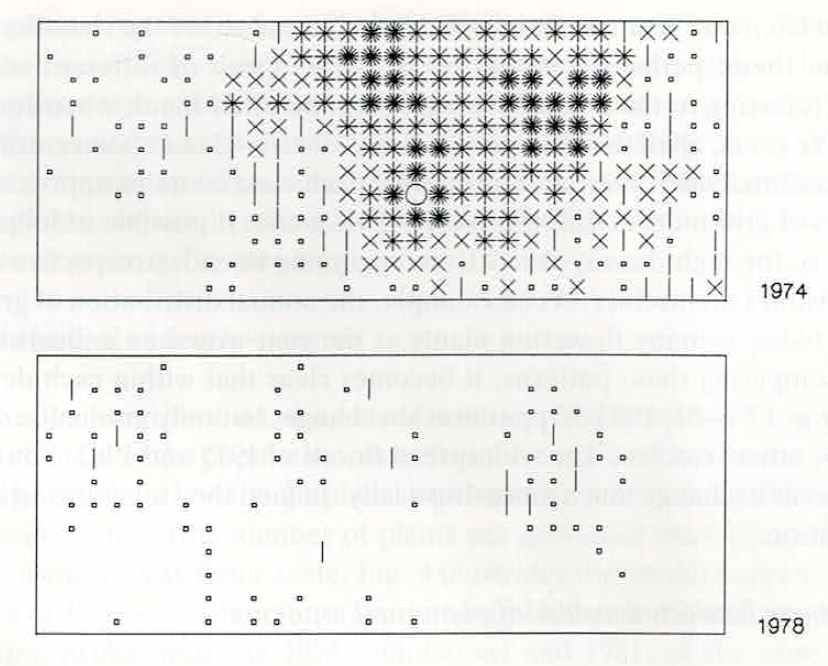
\includegraphics[keepaspectratio]{images/Vanhecke_figure.png}}

}

\caption{\emph{Dactylorhiza praetermissa}; de la publicación}

\end{figure}%

Willems y Bik (Willems \& Bik, 1991) siguieron una población de
\emph{Orchis simia} por 22 años, desde 1968 a 1990, y contabilizan la
cantidad de individuos en cada estado de desarrollo, categorizando estos
como nuevas plantas, plantas fallecidas, con flores, latentes y la
cantidad de plantas totales. Presentan una figura demostrando la
cantidad de individuos en cada estado de desarrollo en el tiempo y
estimando la cantidad de individuos faltantes y muertos.

\section{Evidencia de Google Scholar}\label{evidencia-de-google-scholar}

Haciendo una búsqueda en Google Scholar para
\texttt{"orchid"\ "population\ dynamics"}, se encontró un total de 3,510
artículos. La mayoría de los artículos son revisiones o estudios que no
usan MPP. Miramos los primeros artículos encontrados:

1940-1950

\begin{itemize}
\tightlist
\item
  Carl Olaf Tamm publica el primer artículo sobre dinámica de orquídeas
  en \emph{Botaniska Notiser} (Tamm, 1948). Esta publicación tiene datos
  de \emph{Orchis mascula} y \emph{Orchis sambucina}, entre otras
  especies de plantas en Suecia. Vea el capítulo de Tamm para más
  información.
\end{itemize}

1950-1960 - ninguno

1960-1970 - ninguno

1970-1980

\begin{itemize}
\item
  Margaret Bradshaw (Bradshaw \& Doody, 1978) hace un resumen de los
  valores de estudios de demografía incluyendo orquídeas y menciona los
  trabajos de Tamm (Tamm, 1948, 1972).
\item
  Carl Olaf Tamm (Tamm, 1972) revisó sus análisis de dinámica
  poblacional de \emph{Dactylorhiza sambucina}, \emph{D. incarnata},
  \emph{Orchis mascula} y \emph{Listera ovata}. Estos muestreos
  comenzaron en los años 1940 y se publicaron por primera vez en 1948
  (Tamm, 1948).
\end{itemize}

1980-1990

\begin{itemize}
\item
  Loyal A. Mehrhoff (Mehrhoff, 1989) evaluó la dinámica de \emph{Isotria
  medeoloides} en cinco poblaciones distribuidas entre Georgia (n=2),
  North Carolina (n=2) y South Carolina (n=1), siguiéndolas por seis
  años consecutivos. El autor encontró que la supervivencia de las
  plantas varía entre poblaciones y que las poblaciones tienden a no
  persistir: tres de las cinco habían desaparecido o se habían reducido
  dramáticamente en el periodo de seis años.
\item
  Clare Alexander (Alexander \& Alexander, 1984) comparó el patrón de
  fenología, número de rosetas y supervivencia en \emph{Goodyera repens}
  en tres poblaciones en Inglaterra durante dos años. La autora evaluó
  la longevidad de las rosetas de los individuos y estimó un promedio de
  4.3 ± 1.1 años. Además encontró que la supervivencia de las rosetas
  varía con la densidad: a mayor densidad, menor longevidad. Este
  trabajo pudiese ser el primero que apoya la idea de que la densidad
  influye sobre la supervivencia individual en orquídeas.
\item
  Michael J. Hutchings (Hutchings, 1987) evaluó el efecto del tiempo
  desde la primera vez que una planta emerge sobre su probabilidad de
  florecer en \emph{Ophrys sphegodes} en Inglaterra. Demostró que las
  plantas con mayor edad (tiempo desde el primer avistamiento) florecen
  más, acercándose al 100\% cuando no son latentes. Al contrario, las
  plantas de mayor edad (8 años o más) muestran una reducción en la
  altura de la inflorescencia, el número de hojas y la cantidad de
  flores, apoyando la idea de senescencia. Además, demostró que las
  plantas más robustas (con mayor promedio de flores por año) están
  correlacionadas con la longevidad (\emph{lifespan}).
\item
  Katherine Gregg (Gregg, 1989) estudió la dinámica poblacional de
  \emph{Cleistes divaricata} en tres poblaciones en el este de los
  Estados Unidos. En este trabajo se presenta una revisión de la
  literatura sobre la dinámica poblacional de orquídeas y se discuten
  los métodos usados para estimar la dinámica poblacional. Se presenta
  un análisis de la dinámica poblacional usando MPP y se discute el
  impacto de la latencia en la estimación de los parámetros
  demográficos.
\item
  Ricardo Calvo y Carol C. Horvitz (Calvo \& Horvitz, 1990) estudian la
  dinámica poblacional de \emph{Tolumnia variegata} en Puerto Rico. Se
  presenta un análisis usando MPP y se discute el impacto de la
  variación en transiciones sobre la adecuación demográfica,
  específicamente sobre el efecto de las limitaciones de polinizadores
  sobre la producción de frutos.
\end{itemize}

\begin{center}\rule{0.5\linewidth}{0.5pt}\end{center}

\section{COMPADRE, Orquídea y MPP}\label{compadre-orquuxeddea-y-mpp}

La base de datos de COMPADRE contiene múltiples estudios de dinámica
poblacional en orquídeas y es una buena fuente de información para
estudiar la dinámica poblacional de orquídeas.

\begin{Shaded}
\begin{Highlighting}[]
\NormalTok{compadre }\OtherTok{\textless{}{-}} \FunctionTok{readRDS}\NormalTok{(}\StringTok{"data/COMPADRE\_2026.rds"}\NormalTok{) }\CommentTok{\# Usar este código para bajar los datos del repositorio de COMPADRE. Tiene que haber activado la librería de Rcompadre.}
\end{Highlighting}
\end{Shaded}

\begin{center}\rule{0.5\linewidth}{0.5pt}\end{center}

Cantidad de Familias de plantas en la base de datos de COMPADRE

\begin{Shaded}
\begin{Highlighting}[]
\NormalTok{Familia}\OtherTok{=}\NormalTok{(}\FunctionTok{as.data.frame}\NormalTok{(}\FunctionTok{sort}\NormalTok{(}\FunctionTok{unique}\NormalTok{(compadre}\SpecialCharTok{$}\NormalTok{Family))))}
\FunctionTok{count}\NormalTok{(Familia)}
\end{Highlighting}
\end{Shaded}

\begin{center}\rule{0.5\linewidth}{0.5pt}\end{center}

La cantidad de géneros en la base de datos de COMPADRE

\begin{Shaded}
\begin{Highlighting}[]
\NormalTok{Genera}\OtherTok{=}\NormalTok{(}\FunctionTok{as.data.frame}\NormalTok{(}\FunctionTok{sort}\NormalTok{(}\FunctionTok{unique}\NormalTok{(compadre}\SpecialCharTok{$}\NormalTok{Genus))))}

\FunctionTok{count}\NormalTok{(Genera)}
\end{Highlighting}
\end{Shaded}

\begin{center}\rule{0.5\linewidth}{0.5pt}\end{center}

La cantidad de especies en la base de datos de COMPADRE

\begin{Shaded}
\begin{Highlighting}[]
\NormalTok{Especies}\OtherTok{=}\FunctionTok{as.data.frame}\NormalTok{(}\FunctionTok{sort}\NormalTok{(}\FunctionTok{unique}\NormalTok{(compadre}\SpecialCharTok{$}\NormalTok{SpeciesAccepted)))}

\FunctionTok{count}\NormalTok{(Especies)}
\end{Highlighting}
\end{Shaded}

\begin{center}\rule{0.5\linewidth}{0.5pt}\end{center}

\subsection{\texorpdfstring{Filtrar para la familia
\emph{Orchidaceae}}{Filtrar para la familia Orchidaceae}}\label{filtrar-para-la-familia-orchidaceae-1}

Aquí enseñamos cómo filtrar la base de datos de COMPADRE para obtener
solamente las especies de la familia \emph{Orchidaceae}. En este caso se
usa el paquete \texttt{dplyr} para filtrar y contar las especies únicas
de orquídeas.

\begin{Shaded}
\begin{Highlighting}[]
\NormalTok{Lista\_Orquidea}\OtherTok{=}\NormalTok{compadre }\SpecialCharTok{\%\textgreater{}\%} \FunctionTok{filter}\NormalTok{(Family }\SpecialCharTok{\%in\%} \FunctionTok{c}\NormalTok{(}\StringTok{"Orchidaceae"}\NormalTok{)) }

\NormalTok{Lista\_O}\OtherTok{=}\FunctionTok{as.data.frame}\NormalTok{(}\FunctionTok{sort}\NormalTok{(}\FunctionTok{unique}\NormalTok{(Lista\_Orquidea}\SpecialCharTok{$}\NormalTok{SpeciesAccepted))) }

\FunctionTok{count}\NormalTok{(Lista\_O)}
\end{Highlighting}
\end{Shaded}

\begin{center}\rule{0.5\linewidth}{0.5pt}\end{center}

\begin{Shaded}
\begin{Highlighting}[]
\NormalTok{SPECIES\_Number}\OtherTok{=}\NormalTok{Lista\_Orquidea}\SpecialCharTok{\%\textgreater{}\%} \FunctionTok{select}\NormalTok{(Family, StudyStart, StudyEnd, SpeciesAccepted, YearPublication, Authors, DOI\_ISBN, OrganismType, MatrixPopulation, mat) }\SpecialCharTok{\%\textgreater{}\%} 
  \FunctionTok{group\_by}\NormalTok{(Family) }\SpecialCharTok{\%\textgreater{}\%} 
  \FunctionTok{summarize}\NormalTok{(}\AttributeTok{n\_species =} \FunctionTok{length}\NormalTok{(}\FunctionTok{unique}\NormalTok{(SpeciesAccepted))) }\SpecialCharTok{\%\textgreater{}\%} 
  \FunctionTok{arrange}\NormalTok{(}\FunctionTok{desc}\NormalTok{(n\_species))}

\FunctionTok{summary}\NormalTok{(SPECIES\_Number)}
\end{Highlighting}
\end{Shaded}

\chapter{Carl Olaf Tamm}\label{OTamm}

Carl\,Olaf\,Tamm fue una figura clave en el desarrollo temprano de la
ecología poblacional y del estudio demográfico de plantas. Este capítulo
presenta su contribución científica en el contexto del surgimiento de
enfoques modernos para comprender la dinámica poblacional en sistemas
naturales.

Por: Raymond L. Tremblay

\section{Carl Olaf Tamm y el estudio demográfico de poblaciones
naturales}\label{carl-olaf-tamm-y-el-estudio-demogruxe1fico-de-poblaciones-naturales}

Carl Olaf Tamm desempeñó un papel fundamental en la consolidación de
enfoques demográficos aplicados al estudio de poblaciones vegetales,
particularmente en sistemas naturales de larga duración. Su trabajo se
distinguió por la integración rigurosa de observaciones de campo a largo
plazo con preguntas conceptuales sobre crecimiento, persistencia y
estructura poblacional.

En este capítulo se examinan las principales contribuciones de Tamm al
desarrollo de la ecología poblacional, destacando cómo sus estudios
empíricos proporcionaron una base sólida para enfoques cuantitativos
posteriores. Su énfasis en el seguimiento individual, la variabilidad
interanual y la interpretación biológica de los patrones poblacionales
influyó profundamente en la manera en que se conceptualizan hoy los
procesos demográficos.

A diferencia de los capítulos analíticos del libro, este capítulo se
centra en un \textbf{caso histórico concreto} que ilustra cómo las ideas
y métodos de la dinámica poblacional emergieron a partir de datos reales
y observaciones prolongadas en el tiempo. El trabajo de Tamm sirve como
puente entre la historia del pensamiento ecológico y las herramientas
modernas de análisis matricial, elasticidad y simulación desarrolladas
en capítulos anteriores, mostrando el valor perdurable de los estudios
de campo de largo plazo en la ecología poblacional. El énfasis de Tamm
en el seguimiento empírico prolongado se relaciona directamente con los
principios de recopilación de datos en el campo. Las observaciones de
Tamm anticipan conceptos centrales desarrollados en los capítulos sobre
transiciones demográficas y dinámica de transiciones.

\section{Contexto histórico y principales aportes
científicos}\label{contexto-histuxf3rico-y-principales-aportes-cientuxedficos}

A continuación se presentan los principales aspectos de la trayectoria
científica de Carl Olaf Tamm y su impacto en el desarrollo de la
ecología poblacional.

\subsubsection{Librerías de R requeridas para el siguiente
módulo}\label{libreruxedas-de-r-requeridas-para-el-siguiente-muxf3dulo-18}

\begin{Shaded}
\begin{Highlighting}[]
\ControlFlowTok{if}\NormalTok{ (}\SpecialCharTok{!}\FunctionTok{require}\NormalTok{(}\StringTok{"pacman"}\NormalTok{)) }\FunctionTok{install.packages}\NormalTok{(}\StringTok{"pacman"}\NormalTok{)}
\NormalTok{pacman}\SpecialCharTok{::}\FunctionTok{p\_load}\NormalTok{(janitor, tidyverse, popbio, knitr, flextable)}

\FunctionTok{library}\NormalTok{(tidyverse)}
\FunctionTok{library}\NormalTok{(janitor)}
\FunctionTok{library}\NormalTok{(popbio)}
\FunctionTok{library}\NormalTok{(knitr)}
\FunctionTok{library}\NormalTok{(tidyverse)}
\FunctionTok{library}\NormalTok{(readxl)}
\FunctionTok{library}\NormalTok{(Rage)}
\FunctionTok{library}\NormalTok{(DiagrammeR)}
\FunctionTok{library}\NormalTok{(raretrans) }\CommentTok{\# disponible en CRAN: install.packages("raretrans")}

\CommentTok{\# Mi tema de formato de las gráficas de ggplot2 personal}

\NormalTok{rlt\_theme }\OtherTok{\textless{}{-}} \FunctionTok{theme}\NormalTok{(}
  \AttributeTok{axis.title.y =} \FunctionTok{element\_text}\NormalTok{(}\AttributeTok{colour =} \StringTok{"grey20"}\NormalTok{, }\AttributeTok{size =} \DecValTok{10}\NormalTok{, }\AttributeTok{face =} \StringTok{"bold"}\NormalTok{),}
  \AttributeTok{axis.text.x =} \FunctionTok{element\_text}\NormalTok{(}\AttributeTok{colour =} \StringTok{"grey20"}\NormalTok{, }\AttributeTok{size =} \DecValTok{10}\NormalTok{, }\AttributeTok{face =} \StringTok{"bold"}\NormalTok{),}
  \AttributeTok{axis.text.y =} \FunctionTok{element\_text}\NormalTok{(}\AttributeTok{colour =} \StringTok{"grey20"}\NormalTok{, }\AttributeTok{size =} \DecValTok{15}\NormalTok{, }\AttributeTok{face =} \StringTok{"bold"}\NormalTok{),}
  \AttributeTok{axis.title.x =} \FunctionTok{element\_text}\NormalTok{(}\AttributeTok{colour =} \StringTok{"grey20"}\NormalTok{, }\AttributeTok{size =} \DecValTok{15}\NormalTok{, }\AttributeTok{face =} \StringTok{"bold"}\NormalTok{)}
\NormalTok{) }\SpecialCharTok{+}
  \FunctionTok{theme}\NormalTok{(}
    \CommentTok{\# Remover los bordes}
    \AttributeTok{panel.border =} \FunctionTok{element\_blank}\NormalTok{(),}
    \CommentTok{\# Remover las líneas}
    \AttributeTok{panel.grid.major =} \FunctionTok{element\_blank}\NormalTok{(),}
    \AttributeTok{panel.grid.minor =} \FunctionTok{element\_blank}\NormalTok{(),}
    \CommentTok{\# Remover el fondo del panel}
    \AttributeTok{panel.background =} \FunctionTok{element\_blank}\NormalTok{(),}
    \CommentTok{\# añadir lineas más gruesas}
    \AttributeTok{axis.line.x =} \FunctionTok{element\_line}\NormalTok{(}\AttributeTok{colour =} \StringTok{"black"}\NormalTok{, }\AttributeTok{linewidth =} \DecValTok{1}\NormalTok{),}
    \AttributeTok{axis.line.y =} \FunctionTok{element\_line}\NormalTok{(}\AttributeTok{colour =} \StringTok{"black"}\NormalTok{, }\AttributeTok{linewidth =} \DecValTok{1}\NormalTok{)}
\NormalTok{  )}

\NormalTok{diverging}\OtherTok{=} \FunctionTok{c}\NormalTok{(}\StringTok{"\#009392"}\NormalTok{,}\StringTok{"\#CF597E"}\NormalTok{,}\StringTok{"\#E9E29C"}\NormalTok{, }\StringTok{"\#39B185"}\NormalTok{,}\StringTok{"\#EEB479"}\NormalTok{ , }\StringTok{"\#9CCB86"}\NormalTok{ )}

\CommentTok{\# {-}{-}{-} 2. Combinarlos en un objeto de tipo lista {-}{-}{-}}
\CommentTok{\# Esta lista se puede añadir al gráfico con un solo \textquotesingle{}+\textquotesingle{}}
\NormalTok{rlt\_style\_fill }\OtherTok{\textless{}{-}} \ControlFlowTok{function}\NormalTok{() \{}
  \FunctionTok{list}\NormalTok{(}
\NormalTok{    rlt\_theme,}
    \FunctionTok{scale\_fill\_manual}\NormalTok{(}\AttributeTok{values =}\NormalTok{ diverging)}
\NormalTok{  )}
\NormalTok{\}}

\NormalTok{rlt\_style\_colour }\OtherTok{\textless{}{-}} \ControlFlowTok{function}\NormalTok{() \{}
  \FunctionTok{list}\NormalTok{(}
\NormalTok{    rlt\_theme,}
    \FunctionTok{scale\_colour\_manual}\NormalTok{(}\AttributeTok{values =}\NormalTok{ diverging)}
\NormalTok{  )}
\NormalTok{\}}
\end{Highlighting}
\end{Shaded}

\section{El padre de la ecología de poblaciones en
orquídeas}\label{el-padre-de-la-ecologuxeda-de-poblaciones-en-orquuxeddeas}

Carl Olaf Tamm (1919--2007) fue un biólogo sueco que enseñó en la Royal
College of Forestry de Estocolmo, donde ocupó la cátedra de Soil Science
(Ciencia del Suelo) entre 1957 y 1962, y posteriormente fue el primer
profesor de \textbf{Ecología de Bosques} de dicha institución, cargo que
mantuvo hasta 1985. Los trabajos de Tamm son reconocidos por proyectos a
largo plazo, de múltiples años y décadas, donde él enfatizó la
importancia de la variabilidad temporal y espacial en los ecosistemas,
así como los eventos raros en la dinámica de especies. Tamm desarrolló
protocolos de muestreo de plantas y suelos en bosques, con recolección
de datos anual y continua. Algunos de estos trabajos hoy en día son
conocidos como clásicos en ecología de poblaciones y comunidades. Tres
de estos trabajos relevantes a la dinámica poblacional son los
siguientes:

\begin{itemize}
\item
  Observation on reproduction and survival of some perennial herbs
  (Tamm, 1948).
\item
  Further observations on the survival and flowering of some perennial
  herbs, I (Tamm, 1956).
\item
  Survival and flowering of some perennial herbs. II. The behaviour of
  some orchids on permanent plots (Tamm, 1972).
\end{itemize}

En la descripción de la dinámica de los individuos muestreados a través
del tiempo, Tamm pudo observar la variabilidad temporal en la
reproducción y supervivencia de las plantas, basándose en su presencia o
ausencia, su estado reproductivo, el reclutamiento, la existencia de
individuos clonales y si las plantas eran latentes. Él utilizó un
sistema de presentación de la dinámica de los individuos usando una
línea por individuo e identificando en qué etapa estaba en cada año.

\begin{center}\rule{0.5\linewidth}{0.5pt}\end{center}

Representación visual de los datos de Tamm

Los datos de Tamm fueron compartidos de forma visual usando gráficos. En
la figura cada línea vertical representa un individuo

\begin{itemize}
\tightlist
\item
  línea gruesa, individuo reproductivo
\item
  línea fina, individuo vegetativo
\item
  línea entrecortada: individuo no muestreado
\item
  línea bifurcada: individuos que se clonan
\end{itemize}

\begin{tcolorbox}[enhanced jigsaw, arc=.35mm, bottomrule=.15mm, bottomtitle=1mm, breakable, colback=white, colbacktitle=quarto-callout-tip-color!10!white, colframe=quarto-callout-tip-color-frame, coltitle=black, left=2mm, leftrule=.75mm, opacityback=0, opacitybacktitle=0.6, rightrule=.15mm, title=\textcolor{quarto-callout-tip-color}{\faLightbulb}\hspace{0.5em}{Recomendación}, titlerule=0mm, toprule=.15mm, toptitle=1mm]

\textbf{El método visual de Tamm sigue vigente.} El diagrama de líneas
verticales ---una por individuo, con grosor codificando estado
reproductivo y discontinuidades indicando años no muestreados--- es
esencialmente una representación cruda de un \emph{capture-recapture
history}. Mucho antes de que existieran los modelos formales de
Cormack-Jolly-Seber, Tamm intuyó que la unidad básica del análisis
demográfico es la \textbf{historia de cada individuo}, no el conteo
agregado. Los métodos bayesianos modernos para estimar latencia
(capítulo de
\hyperref[acercamiento-bayesiano-para-calcular-transiciones-y-fecundidades]{Acercamiento
bayesiano}) son la formalización estadística de lo que Tamm ya hacía
visualmente.

\end{tcolorbox}

\begin{figure}[H]

{\centering 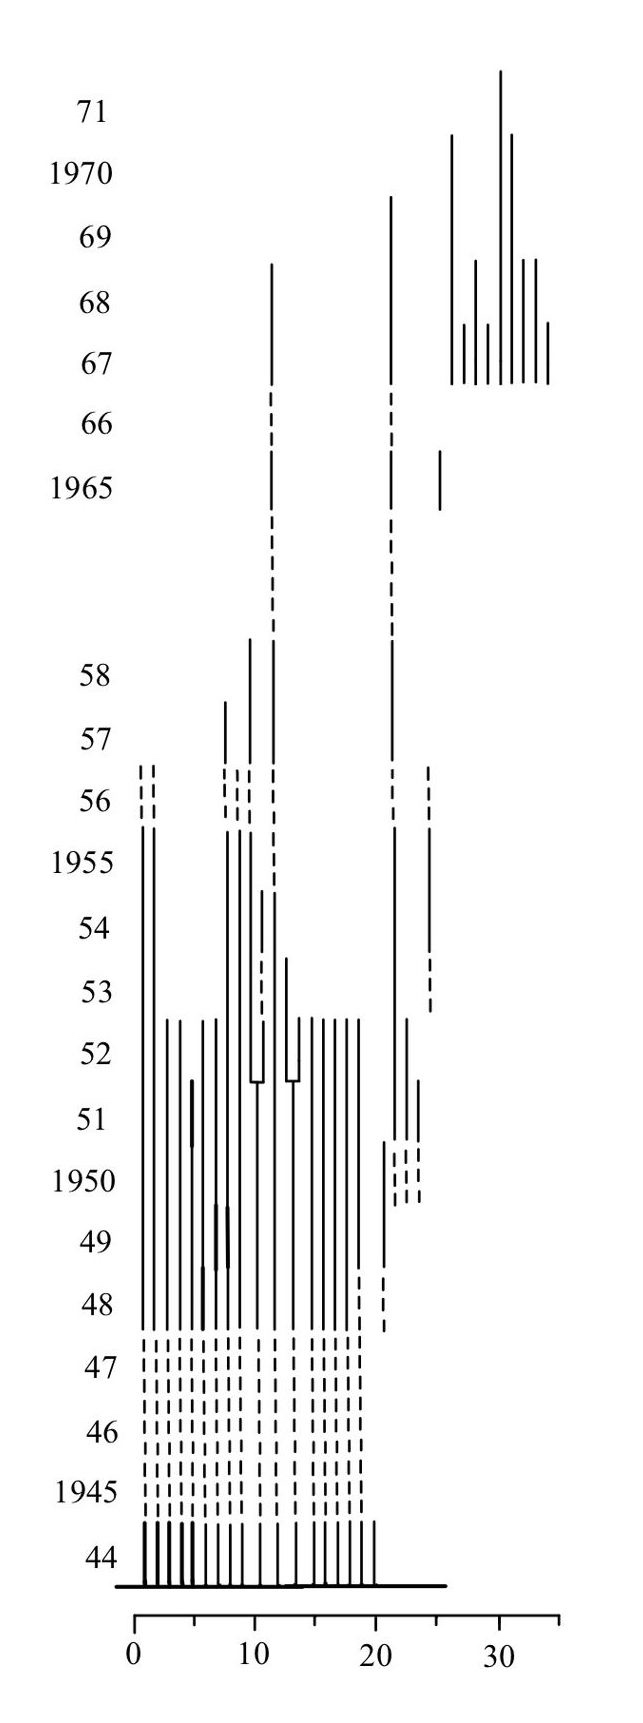
\includegraphics[width=0.5\linewidth,height=\textheight,keepaspectratio]{images/Tamm_1972_Dactylorhiza_incarnata_2.jpeg}

}

\caption{Reproducción de Tamm: 1972, Dactylorhiza incarnata, dibujo por
Alondra Martinez Martinez}

\end{figure}%

Tamm estableció en el campo parcelas de 0.5 m × 0.5 m o de 1.0 m × 1.0 m
y muestreó todos los individuos en cada parcela en años consecutivos
(las líneas entrecortadas son años no muestreados). Por ejemplo, entre
1945 y 1947 no se muestreó esta parcela a causa de la Segunda Guerra
Mundial. Tamm estaba interesado en la dinámica de las orquídeas porque
había notado que los individuos no florecen todos los años, y que la
floración era un evento relativamente raro. En \emph{Orchis sambucina}
(ahora \emph{Dactylorhiza sambucina}) notó que en 1942 solamente 7
plantas florecieron, mientras que en 1945 había 40 con flores (Tamm,
1948). Tamm sugirió que la poca cantidad de nuevos individuos podría
estar correlacionada con la competencia por recursos (nutrientes, luz y
agua), y que la capacidad de las plantas de sobrevivir eventos difíciles
está parcialmente correlacionada con su edad: las plantas de mayor edad
podrían tener una menor probabilidad de supervivencia (Tamm, 1948). Tamm
sugirió, además, que las plantas tienen un límite de años que pueden
sobrevivir, es decir que existe senescencia en plantas perennes. Aunque
ese concepto estaba bien establecido en animales, no se había
considerado seriamente en plantas perennes hasta entonces.

\begin{tcolorbox}[enhanced jigsaw, arc=.35mm, bottomrule=.15mm, bottomtitle=1mm, breakable, colback=white, colbacktitle=quarto-callout-note-color!10!white, colframe=quarto-callout-note-color-frame, coltitle=black, left=2mm, leftrule=.75mm, opacityback=0, opacitybacktitle=0.6, rightrule=.15mm, title=\textcolor{quarto-callout-note-color}{\faInfo}\hspace{0.5em}{Nota}, titlerule=0mm, toprule=.15mm, toptitle=1mm]

\textbf{Senescencia en plantas perennes: una idea que tardó en
aceptarse.} Tamm propuso que las orquídeas terrestres muestran
senescencia ---la probabilidad de morir aumenta con la edad--- una idea
que en la década de 1940 era controvertida. Muchos botánicos asumían que
las plantas perennes podían vivir indefinidamente bajo condiciones
favorables. Estudios posteriores con orquídeas y otras plantas perennes
han confirmado el patrón en algunas especies, pero también han mostrado
que la longevidad puede variar enormemente entre especies, lo cual hace
difícil generalizar (ver (Tremblay, 2000) para \emph{Lepanthes}).

\end{tcolorbox}

\begin{figure}[H]

{\centering \pandocbounded{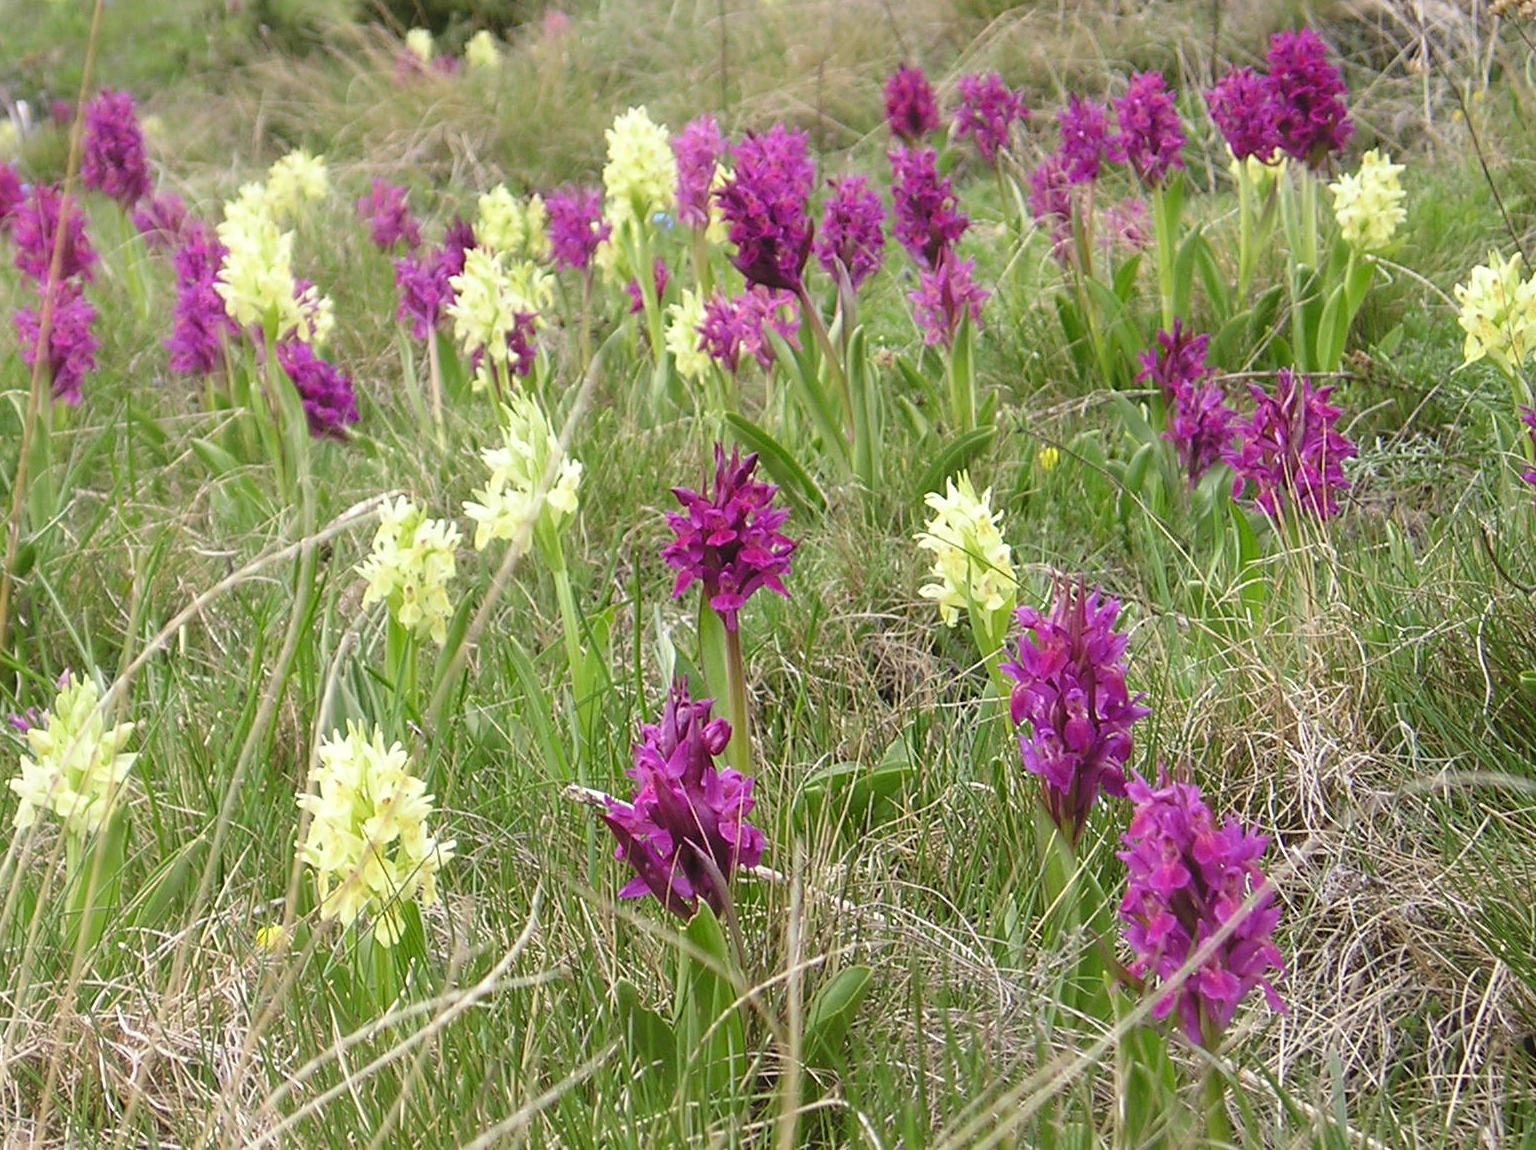
\includegraphics[keepaspectratio]{images/Dactylorhiza_sambucina_James_D._Ackerman.jpg}}

}

\caption{\emph{Dactylorhiza sambucina}. Foto: James D. Ackerman}

\end{figure}%

\begin{center}\rule{0.5\linewidth}{0.5pt}\end{center}

En la siguiente figura se muestra la dinámica de los individuos de
\emph{Listera ovata} muestreados por Tamm desde 1944 a 1971 (Tamm,
1972). En esta figura se puede ver la variabilidad temporal en la
reproducción y supervivencia de las plantas, según su presencia o
ausencia, si eran reproductivas o no, el reclutamiento, los individuos
que se clonan y si las plantas estaban latentes. Él utilizó un sistema
de presentación de la dinámica de los individuos usando una línea por
individuo e identificando en qué etapa estaba en cada año. El sitio
(plot 48) es bosque mésico con un dosel casi cerrado.

\begin{figure}[H]

{\centering 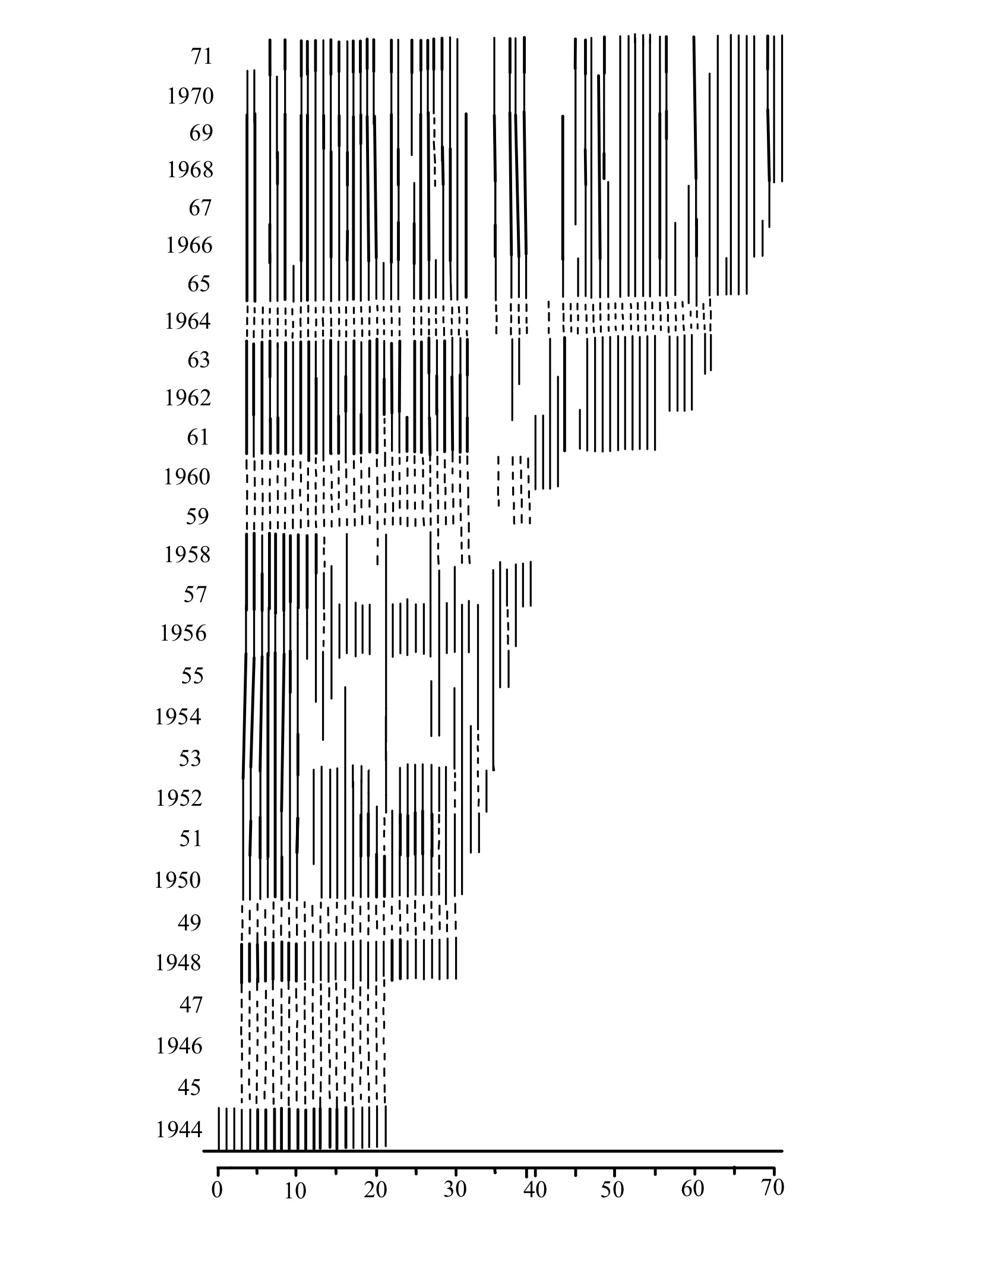
\includegraphics[width=0.5\linewidth,height=\textheight,keepaspectratio]{images/Tamm_1972_plot_48.jpeg}

}

\caption{Dinámica del plot 48: Listera ovata, dibujo por Alondra
Martínez Martínez}

\end{figure}%

\begin{center}\rule{0.5\linewidth}{0.5pt}\end{center}

En la publicación de 1972 (Tamm, 1972), Tamm describe la dinámica de
múltiples especies de orquídeas, y algunas especies en múltiples sitios.

\global\setlength{\Oldarrayrulewidth}{\arrayrulewidth}

\global\setlength{\Oldtabcolsep}{\tabcolsep}

\setlength{\tabcolsep}{2pt}

\renewcommand*{\arraystretch}{1.5}



\providecommand{\ascline}[3]{\noalign{\global\arrayrulewidth #1}\arrayrulecolor[HTML]{#2}\cline{#3}}

\begin{longtable*}[c]{cccc}



\ascline{1.5pt}{666666}{1-4}

\multicolumn{1}{>{}l}{\textcolor[HTML]{000000}{\fontsize{11}{11}\selectfont{Especies}}} & \multicolumn{1}{>{}r}{\textcolor[HTML]{000000}{\fontsize{11}{11}\selectfont{Núm\ de\ la\ Población}}} & \multicolumn{1}{>{}r}{\textcolor[HTML]{000000}{\fontsize{11}{11}\selectfont{Año\ del\ primer\ muestreo}}} & \multicolumn{1}{>{}r}{\textcolor[HTML]{000000}{\fontsize{11}{11}\selectfont{Año\ del\ último\ muestreo}}} \\

\ascline{1.5pt}{666666}{1-4}\endfirsthead 

\ascline{1.5pt}{666666}{1-4}

\multicolumn{1}{>{}l}{\textcolor[HTML]{000000}{\fontsize{11}{11}\selectfont{Especies}}} & \multicolumn{1}{>{}r}{\textcolor[HTML]{000000}{\fontsize{11}{11}\selectfont{Núm\ de\ la\ Población}}} & \multicolumn{1}{>{}r}{\textcolor[HTML]{000000}{\fontsize{11}{11}\selectfont{Año\ del\ primer\ muestreo}}} & \multicolumn{1}{>{}r}{\textcolor[HTML]{000000}{\fontsize{11}{11}\selectfont{Año\ del\ último\ muestreo}}} \\

\ascline{1.5pt}{666666}{1-4}\endhead



\multicolumn{1}{>{}l}{\textcolor[HTML]{000000}{\fontsize{11}{11}\selectfont{Dactylorhiza\ incarnata}}} & \multicolumn{1}{>{}r}{\textcolor[HTML]{000000}{\fontsize{11}{11}\selectfont{46}}} & \multicolumn{1}{>{}r}{\textcolor[HTML]{000000}{\fontsize{11}{11}\selectfont{1,944}}} & \multicolumn{1}{>{}r}{\textcolor[HTML]{000000}{\fontsize{11}{11}\selectfont{1,971}}} \\





\multicolumn{1}{>{}l}{\textcolor[HTML]{000000}{\fontsize{11}{11}\selectfont{Dactylorhiza\ sambucina}}} & \multicolumn{1}{>{}r}{\textcolor[HTML]{000000}{\fontsize{11}{11}\selectfont{17}}} & \multicolumn{1}{>{}r}{\textcolor[HTML]{000000}{\fontsize{11}{11}\selectfont{1,942}}} & \multicolumn{1}{>{}r}{\textcolor[HTML]{000000}{\fontsize{11}{11}\selectfont{1,971}}} \\





\multicolumn{1}{>{}l}{\textcolor[HTML]{000000}{\fontsize{11}{11}\selectfont{Dactylorhiza\ sambucina}}} & \multicolumn{1}{>{}r}{\textcolor[HTML]{000000}{\fontsize{11}{11}\selectfont{18}}} & \multicolumn{1}{>{}r}{\textcolor[HTML]{000000}{\fontsize{11}{11}\selectfont{1,943}}} & \multicolumn{1}{>{}r}{\textcolor[HTML]{000000}{\fontsize{11}{11}\selectfont{1,964}}} \\





\multicolumn{1}{>{}l}{\textcolor[HTML]{000000}{\fontsize{11}{11}\selectfont{Dactylorhiza\ sambucina}}} & \multicolumn{1}{>{}r}{\textcolor[HTML]{000000}{\fontsize{11}{11}\selectfont{19}}} & \multicolumn{1}{>{}r}{\textcolor[HTML]{000000}{\fontsize{11}{11}\selectfont{1,943}}} & \multicolumn{1}{>{}r}{\textcolor[HTML]{000000}{\fontsize{11}{11}\selectfont{1,957}}} \\





\multicolumn{1}{>{}l}{\textcolor[HTML]{000000}{\fontsize{11}{11}\selectfont{Dactylorhiza\ sambucina}}} & \multicolumn{1}{>{}r}{\textcolor[HTML]{000000}{\fontsize{11}{11}\selectfont{20}}} & \multicolumn{1}{>{}r}{\textcolor[HTML]{000000}{\fontsize{11}{11}\selectfont{1,943}}} & \multicolumn{1}{>{}r}{\textcolor[HTML]{000000}{\fontsize{11}{11}\selectfont{1,957}}} \\





\multicolumn{1}{>{}l}{\textcolor[HTML]{000000}{\fontsize{11}{11}\selectfont{Dactylorhiza\ sambucina}}} & \multicolumn{1}{>{}r}{\textcolor[HTML]{000000}{\fontsize{11}{11}\selectfont{21}}} & \multicolumn{1}{>{}r}{\textcolor[HTML]{000000}{\fontsize{11}{11}\selectfont{1,943}}} & \multicolumn{1}{>{}r}{\textcolor[HTML]{000000}{\fontsize{11}{11}\selectfont{1,957}}} \\





\multicolumn{1}{>{}l}{\textcolor[HTML]{000000}{\fontsize{11}{11}\selectfont{Dactylorhiza\ sambucina}}} & \multicolumn{1}{>{}r}{\textcolor[HTML]{000000}{\fontsize{11}{11}\selectfont{22}}} & \multicolumn{1}{>{}r}{\textcolor[HTML]{000000}{\fontsize{11}{11}\selectfont{1,943}}} & \multicolumn{1}{>{}r}{\textcolor[HTML]{000000}{\fontsize{11}{11}\selectfont{1,957}}} \\





\multicolumn{1}{>{}l}{\textcolor[HTML]{000000}{\fontsize{11}{11}\selectfont{Orchis\ mascula}}} & \multicolumn{1}{>{}r}{\textcolor[HTML]{000000}{\fontsize{11}{11}\selectfont{24}}} & \multicolumn{1}{>{}r}{\textcolor[HTML]{000000}{\fontsize{11}{11}\selectfont{1,943}}} & \multicolumn{1}{>{}r}{\textcolor[HTML]{000000}{\fontsize{11}{11}\selectfont{1,956}}} \\





\multicolumn{1}{>{}l}{\textcolor[HTML]{000000}{\fontsize{11}{11}\selectfont{Listera\ ovata}}} & \multicolumn{1}{>{}r}{\textcolor[HTML]{000000}{\fontsize{11}{11}\selectfont{48}}} & \multicolumn{1}{>{}r}{\textcolor[HTML]{000000}{\fontsize{11}{11}\selectfont{1,944}}} & \multicolumn{1}{>{}r}{\textcolor[HTML]{000000}{\fontsize{11}{11}\selectfont{1,971}}} \\

\ascline{1.5pt}{666666}{1-4}



\end{longtable*}



\arrayrulecolor[HTML]{000000}

\global\setlength{\arrayrulewidth}{\Oldarrayrulewidth}

\global\setlength{\tabcolsep}{\Oldtabcolsep}

\renewcommand*{\arraystretch}{1}

En la publicación de 1972, Tamm describió la dinámica de cuatro especies
de orquídeas. Esta información no está disponible en COMPADRE al
momento. En \emph{Dactylorhiza incarnata} se observa que múltiples
individuos desaparecen de un año a otro, y que después de 1951 la
población es mayormente vegetativa (sin flores). Usando las figuras,
Tamm trató de ver si había un patrón en la dinámica basado en el cambio
de las comunidades, por ejemplo la presencia de un árbol de pino que se
estableció cerca de la población de \emph{D. sambucina}. La población de
\emph{D. sambucina} disminuyó un poco entre 1942 y 1963, pero fue
balanceada por el reclutamiento de una cantidad similar de individuos en
el mismo periodo. Después de revisar sus datos, Tamm sugirió que lo que
parecen ser nuevos individuos por clonaje pudieran ser en realidad
individuos independientes, simplemente establecidos muy cerca de un
individuo previo. La dificultad de muestrear con confianza los
individuos en su ambiente es un reto persistente en la interpretación de
los datos de plantas perennes.

\begin{figure}[H]

{\centering \pandocbounded{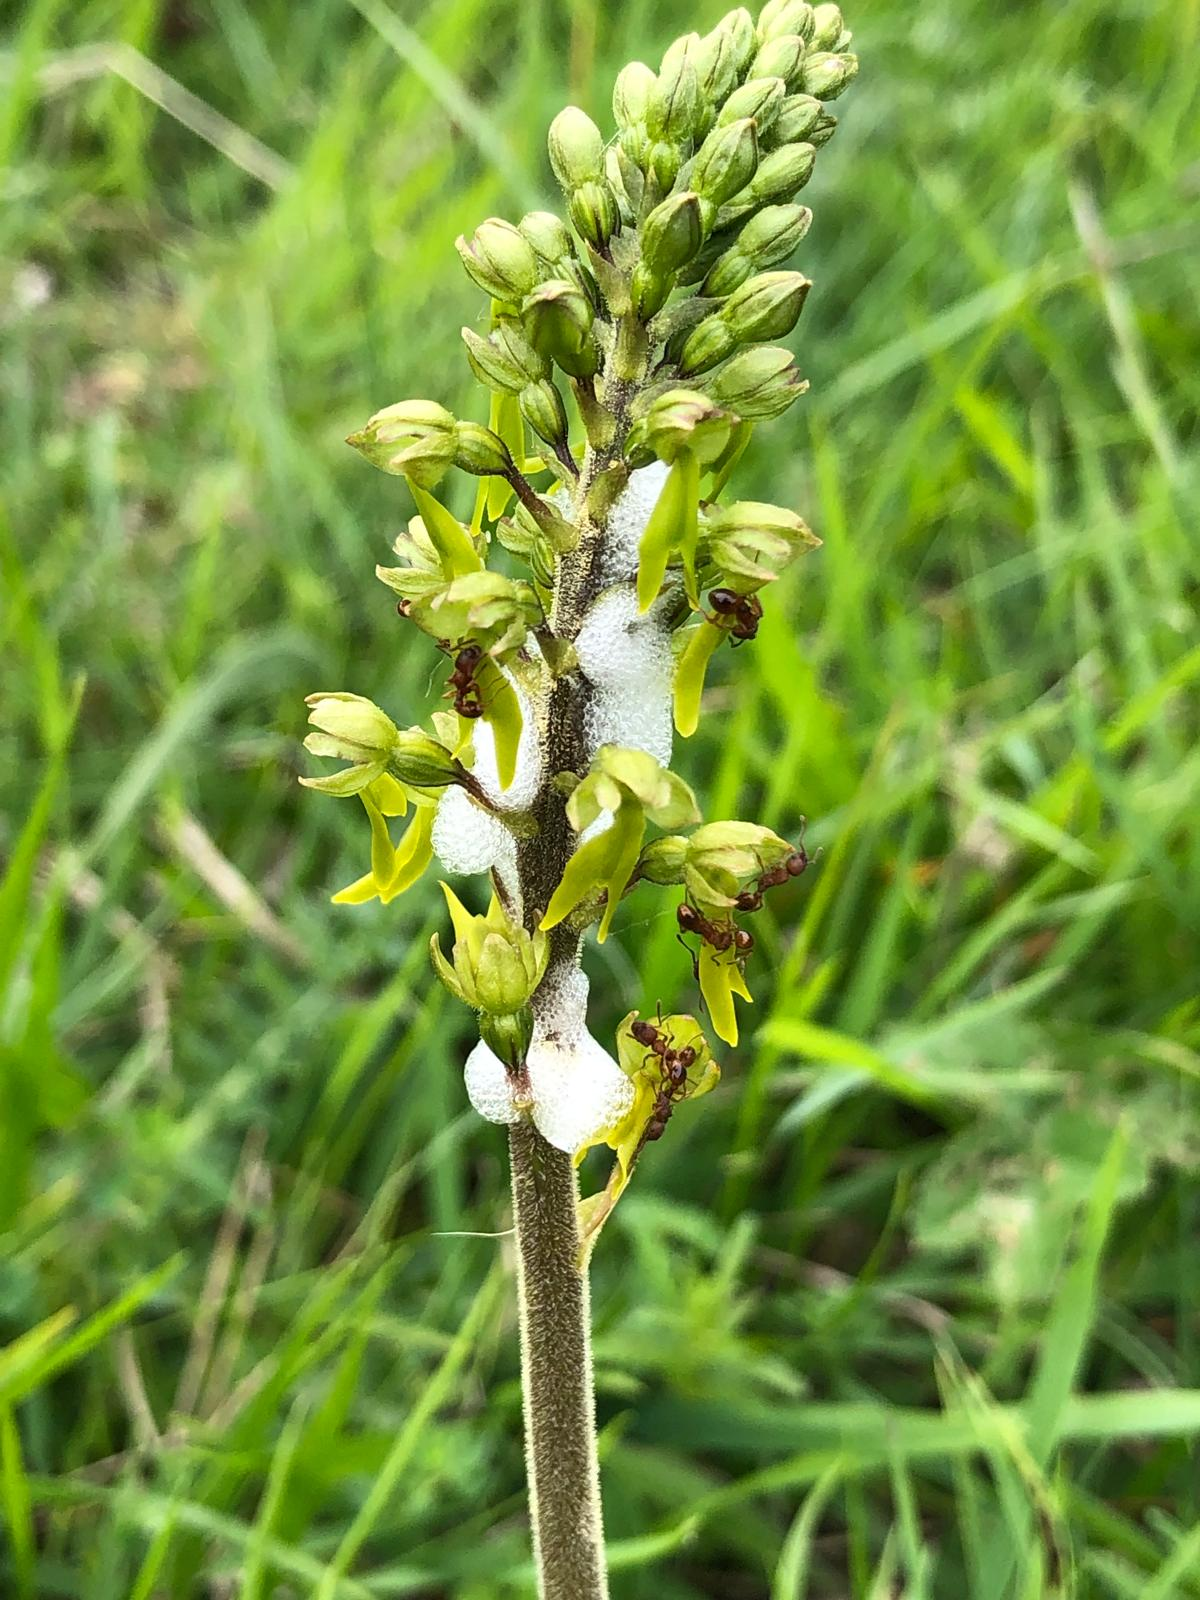
\includegraphics[keepaspectratio]{images/Dactylorhiza_maculata_James_D._Ackerman.jpg}}

}

\caption{\emph{Dactylorhiza maculata con hormigas y spittle bugs}. Foto:
James D. Ackerman}

\end{figure}%

En \emph{Orchis maculata} (ahora \emph{Dactylorhiza maculata}) Tamm
observó claramente que las plantas florecen de forma irregular, con
patrones entre años: algunos años favorecen la presencia de
inflorescencias y otros no. En \emph{Listera ovata}, Tamm observó que la
población creció con mucho reclutamiento entre 1944 y 1971, con un
incremento de más de 200\% comparado con el primer año de muestreo.
Además, demuestra que hay individuos que pueden vivir por muchos años.
La edad de algunos individuos que él muestreó fue de 30 años para
\emph{D. sambucina}, 28 años para \emph{L. ovata}, 25 años para \emph{D.
incarnata} y 14 años para \emph{O. mascula}, demostrando el alto
potencial de longevidad de las orquídeas.

Una de las hipótesis de Tamm es que hay senescencia en las orquídeas. En
otras palabras, la probabilidad de sobrevivir disminuye con la edad. Él
evaluó el patrón de supervivencia en cuatro especies: \emph{Dactylorhiza
incarnata}, \emph{Dactylorhiza sambucina}, \emph{Listera ovata} y
\emph{Orchis mascula}. Usó figuras de supervivencia para evaluar la
probabilidad de sobrevivir de un año a otro en una escala logarítmica.
Tamm predijo que si la supervivencia no está ligada a la edad, la curva
de supervivencia debería seguir una línea recta en escala logarítmica
(mortalidad constante por año) (Tamm, 1972).

\begin{figure}[H]

{\centering 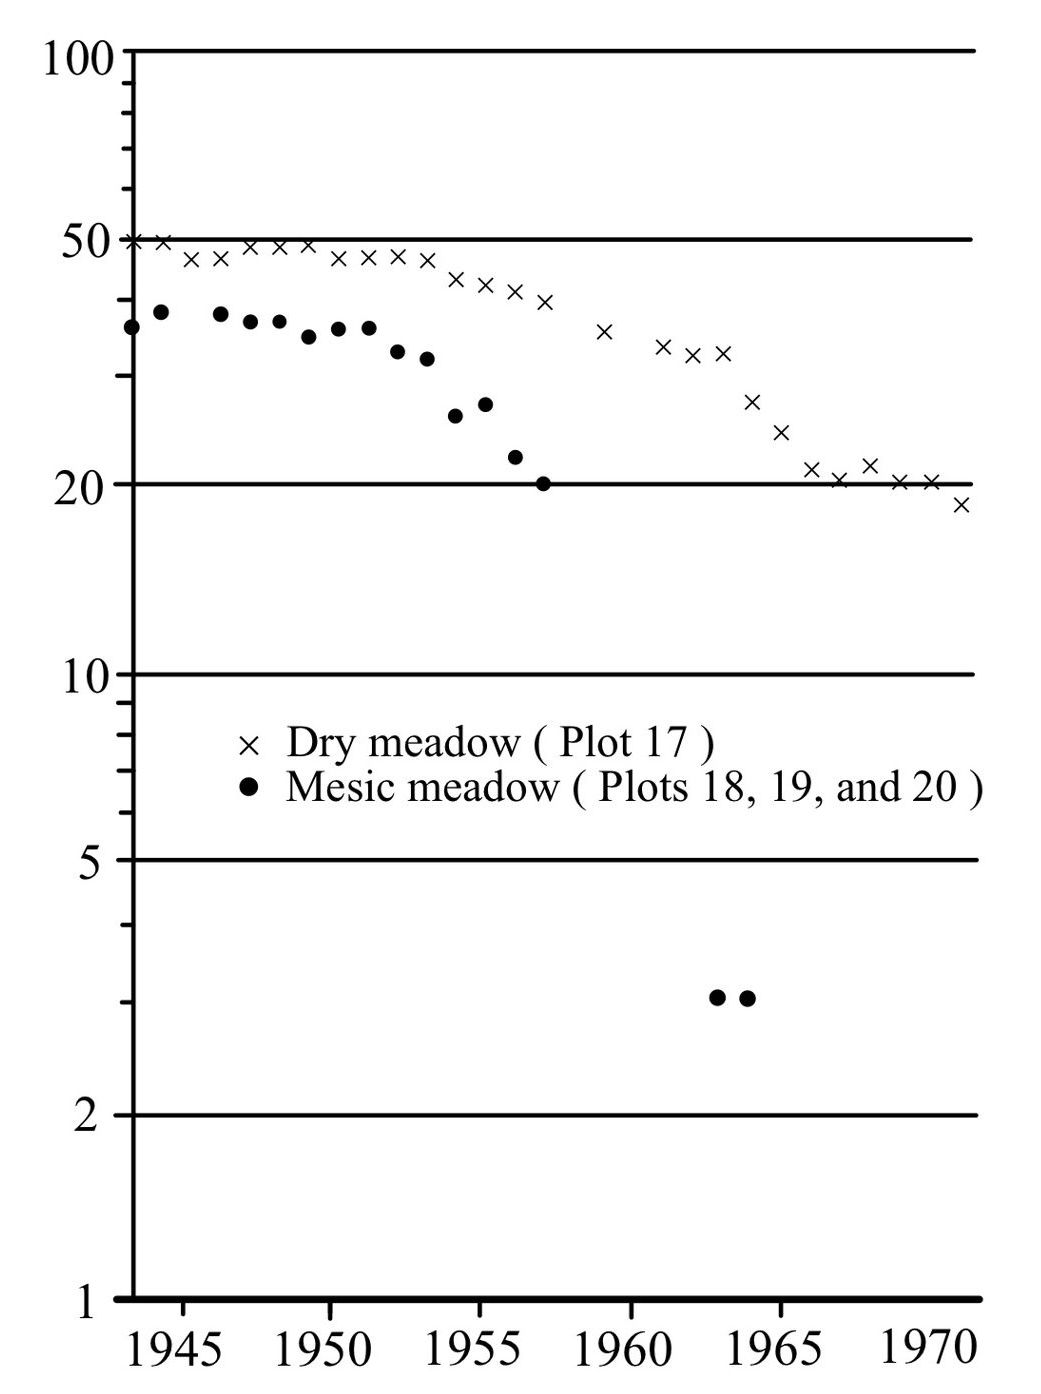
\includegraphics[width=0.65\linewidth,height=\textheight,keepaspectratio]{images/Tamm_D_sambucina_1945_1970_crop.jpeg}

}

\caption{Supervivencia de Dactylorhiza sambucina}

\end{figure}%

En la figura siguiente se enseña la grafica de supervivencia de
\emph{Dactylorhiza sambucina} muestreado por Tamm desde 1944 a 1971
(re-dibujado por Alondra Martínez Martínez).

\begin{center}\rule{0.5\linewidth}{0.5pt}\end{center}

\section{Re-evaluación de los datos de
Tamm}\label{re-evaluaciuxf3n-de-los-datos-de-tamm}

\begin{tcolorbox}[enhanced jigsaw, arc=.35mm, bottomrule=.15mm, bottomtitle=1mm, breakable, colback=white, colbacktitle=quarto-callout-warning-color!10!white, colframe=quarto-callout-warning-color-frame, coltitle=black, left=2mm, leftrule=.75mm, opacityback=0, opacitybacktitle=0.6, rightrule=.15mm, title=\textcolor{quarto-callout-warning-color}{\faExclamationTriangle}\hspace{0.5em}{Advertencia}, titlerule=0mm, toprule=.15mm, toptitle=1mm]

\textbf{Cuidados al re-analizar datos demográficos antiguos.} Re-aplicar
métodos modernos a datos históricos es valioso pero tiene limitaciones:

\begin{itemize}
\tightlist
\item
  \textbf{Definiciones de estadios pueden haber cambiado} (lo que Tamm
  consideraba ``vegetativo'' puede no coincidir exactamente con
  definiciones actuales).
\item
  \textbf{Los datos faltantes} (años no muestreados, individuos
  perdidos) introducen sesgo si se asume que ausencia = muerte.
\item
  \textbf{Los priors deben venir de especies emparentadas o del mismo
  sistema}, no de cualquier especie disponible. Aquí usamos
  \emph{Dactylorhiza lapponica} porque está en COMPADRE, pero las
  dinámicas pueden diferir.
\end{itemize}

Los resultados deben interpretarse como una \textbf{aproximación
coherente}, no como un análisis sustituto del que Tamm hubiera hecho con
métodos modernos.

\end{tcolorbox}

En la próxima sección se re-evaluarán los datos de Tamm con métodos
recientes.

Primero se estará digitalizando los datos, seguido de construcción de
matriz y un análisis sencillo de viabilidad de poblaciones y otras
métricas de dinámica de poblaciones.

\section{Instalación de raretrans}\label{instalaciuxf3n-de-raretrans}

El paquete \textbf{raretrans} está disponible en CRAN y se instala con
\texttt{install.packages()}. Solo es necesario ejecutar esta línea una
vez en la computadora.

\begin{Shaded}
\begin{Highlighting}[]
\FunctionTok{install.packages}\NormalTok{(}\StringTok{"raretrans"}\NormalTok{) }\CommentTok{\# instalar desde CRAN (ejecutar solo una vez)}
\end{Highlighting}
\end{Shaded}

Subir los datos de Tamm

Se puede tener acceso a los datos de Tamm en el archivo
``Tamm\_1972.xlsx'' en la carpeta ``data'' en Github, de este libro.

Estos datos están limitados a la especie \emph{Dactylorhiza incarnata} y
contienen información de los 35 individuos monitoreados desde 1944 hasta
1971.

\begin{Shaded}
\begin{Highlighting}[]
\NormalTok{Tamm\_1972\_column }\OtherTok{\textless{}{-}} \FunctionTok{read\_excel}\NormalTok{(}\StringTok{"data/Tamm\_1972.xlsx"}\NormalTok{, }
    \AttributeTok{sheet =} \StringTok{"D\_incarnata\_by\_column"}\NormalTok{)}

\NormalTok{Tamm\_1972\_column }\SpecialCharTok{\%\textgreater{}\%} \FunctionTok{head}\NormalTok{() }\SpecialCharTok{|\textgreater{}} \FunctionTok{flextable}\NormalTok{()}
\end{Highlighting}
\end{Shaded}

\global\setlength{\Oldarrayrulewidth}{\arrayrulewidth}

\global\setlength{\Oldtabcolsep}{\tabcolsep}

\setlength{\tabcolsep}{2pt}

\renewcommand*{\arraystretch}{1.5}



\providecommand{\ascline}[3]{\noalign{\global\arrayrulewidth #1}\arrayrulecolor[HTML]{#2}\cline{#3}}

\begin{longtable*}[c]{cccccccccccccccccccccccc}



\ascline{1.5pt}{666666}{1-24}

\multicolumn{1}{>{}r}{\textcolor[HTML]{000000}{\fontsize{11}{11}\selectfont{Plant\_Num}}} & \multicolumn{1}{>{}r}{\textcolor[HTML]{000000}{\fontsize{11}{11}\selectfont{Year}}} & \multicolumn{1}{>{}l}{\textcolor[HTML]{000000}{\fontsize{11}{11}\selectfont{stage}}} & \multicolumn{1}{>{}l}{\textcolor[HTML]{000000}{\fontsize{11}{11}\selectfont{next\_stage}}} & \multicolumn{1}{>{}l}{\textcolor[HTML]{000000}{\fontsize{11}{11}\selectfont{1948}}} & \multicolumn{1}{>{}r}{\textcolor[HTML]{000000}{\fontsize{11}{11}\selectfont{Fertility}}} & \multicolumn{1}{>{}l}{\textcolor[HTML]{000000}{\fontsize{11}{11}\selectfont{1949}}} & \multicolumn{1}{>{}l}{\textcolor[HTML]{000000}{\fontsize{11}{11}\selectfont{1950}}} & \multicolumn{1}{>{}l}{\textcolor[HTML]{000000}{\fontsize{11}{11}\selectfont{1951}}} & \multicolumn{1}{>{}l}{\textcolor[HTML]{000000}{\fontsize{11}{11}\selectfont{1952}}} & \multicolumn{1}{>{}l}{\textcolor[HTML]{000000}{\fontsize{11}{11}\selectfont{1953}}} & \multicolumn{1}{>{}l}{\textcolor[HTML]{000000}{\fontsize{11}{11}\selectfont{1954}}} & \multicolumn{1}{>{}l}{\textcolor[HTML]{000000}{\fontsize{11}{11}\selectfont{1955}}} & \multicolumn{1}{>{}l}{\textcolor[HTML]{000000}{\fontsize{11}{11}\selectfont{1956}}} & \multicolumn{1}{>{}l}{\textcolor[HTML]{000000}{\fontsize{11}{11}\selectfont{1957}}} & \multicolumn{1}{>{}l}{\textcolor[HTML]{000000}{\fontsize{11}{11}\selectfont{1958}}} & \multicolumn{1}{>{}l}{\textcolor[HTML]{000000}{\fontsize{11}{11}\selectfont{59-64}}} & \multicolumn{1}{>{}l}{\textcolor[HTML]{000000}{\fontsize{11}{11}\selectfont{1965}}} & \multicolumn{1}{>{}l}{\textcolor[HTML]{000000}{\fontsize{11}{11}\selectfont{1966}}} & \multicolumn{1}{>{}l}{\textcolor[HTML]{000000}{\fontsize{11}{11}\selectfont{1967}}} & \multicolumn{1}{>{}l}{\textcolor[HTML]{000000}{\fontsize{11}{11}\selectfont{1968}}} & \multicolumn{1}{>{}l}{\textcolor[HTML]{000000}{\fontsize{11}{11}\selectfont{1969}}} & \multicolumn{1}{>{}l}{\textcolor[HTML]{000000}{\fontsize{11}{11}\selectfont{1970}}} & \multicolumn{1}{>{}l}{\textcolor[HTML]{000000}{\fontsize{11}{11}\selectfont{1971}}} \\

\ascline{1.5pt}{666666}{1-24}\endfirsthead 

\ascline{1.5pt}{666666}{1-24}

\multicolumn{1}{>{}r}{\textcolor[HTML]{000000}{\fontsize{11}{11}\selectfont{Plant\_Num}}} & \multicolumn{1}{>{}r}{\textcolor[HTML]{000000}{\fontsize{11}{11}\selectfont{Year}}} & \multicolumn{1}{>{}l}{\textcolor[HTML]{000000}{\fontsize{11}{11}\selectfont{stage}}} & \multicolumn{1}{>{}l}{\textcolor[HTML]{000000}{\fontsize{11}{11}\selectfont{next\_stage}}} & \multicolumn{1}{>{}l}{\textcolor[HTML]{000000}{\fontsize{11}{11}\selectfont{1948}}} & \multicolumn{1}{>{}r}{\textcolor[HTML]{000000}{\fontsize{11}{11}\selectfont{Fertility}}} & \multicolumn{1}{>{}l}{\textcolor[HTML]{000000}{\fontsize{11}{11}\selectfont{1949}}} & \multicolumn{1}{>{}l}{\textcolor[HTML]{000000}{\fontsize{11}{11}\selectfont{1950}}} & \multicolumn{1}{>{}l}{\textcolor[HTML]{000000}{\fontsize{11}{11}\selectfont{1951}}} & \multicolumn{1}{>{}l}{\textcolor[HTML]{000000}{\fontsize{11}{11}\selectfont{1952}}} & \multicolumn{1}{>{}l}{\textcolor[HTML]{000000}{\fontsize{11}{11}\selectfont{1953}}} & \multicolumn{1}{>{}l}{\textcolor[HTML]{000000}{\fontsize{11}{11}\selectfont{1954}}} & \multicolumn{1}{>{}l}{\textcolor[HTML]{000000}{\fontsize{11}{11}\selectfont{1955}}} & \multicolumn{1}{>{}l}{\textcolor[HTML]{000000}{\fontsize{11}{11}\selectfont{1956}}} & \multicolumn{1}{>{}l}{\textcolor[HTML]{000000}{\fontsize{11}{11}\selectfont{1957}}} & \multicolumn{1}{>{}l}{\textcolor[HTML]{000000}{\fontsize{11}{11}\selectfont{1958}}} & \multicolumn{1}{>{}l}{\textcolor[HTML]{000000}{\fontsize{11}{11}\selectfont{59-64}}} & \multicolumn{1}{>{}l}{\textcolor[HTML]{000000}{\fontsize{11}{11}\selectfont{1965}}} & \multicolumn{1}{>{}l}{\textcolor[HTML]{000000}{\fontsize{11}{11}\selectfont{1966}}} & \multicolumn{1}{>{}l}{\textcolor[HTML]{000000}{\fontsize{11}{11}\selectfont{1967}}} & \multicolumn{1}{>{}l}{\textcolor[HTML]{000000}{\fontsize{11}{11}\selectfont{1968}}} & \multicolumn{1}{>{}l}{\textcolor[HTML]{000000}{\fontsize{11}{11}\selectfont{1969}}} & \multicolumn{1}{>{}l}{\textcolor[HTML]{000000}{\fontsize{11}{11}\selectfont{1970}}} & \multicolumn{1}{>{}l}{\textcolor[HTML]{000000}{\fontsize{11}{11}\selectfont{1971}}} \\

\ascline{1.5pt}{666666}{1-24}\endhead



\multicolumn{1}{>{}r}{\textcolor[HTML]{000000}{\fontsize{11}{11}\selectfont{1}}} & \multicolumn{1}{>{}r}{\textcolor[HTML]{000000}{\fontsize{11}{11}\selectfont{1,944}}} & \multicolumn{1}{>{}l}{\textcolor[HTML]{000000}{\fontsize{11}{11}\selectfont{F}}} & \multicolumn{1}{>{}l}{\textcolor[HTML]{000000}{\fontsize{11}{11}\selectfont{V}}} & \multicolumn{1}{>{}l}{\textcolor[HTML]{000000}{\fontsize{11}{11}\selectfont{V}}} & \multicolumn{1}{>{}r}{\textcolor[HTML]{000000}{\fontsize{11}{11}\selectfont{0}}} & \multicolumn{1}{>{}l}{\textcolor[HTML]{000000}{\fontsize{11}{11}\selectfont{V}}} & \multicolumn{1}{>{}l}{\textcolor[HTML]{000000}{\fontsize{11}{11}\selectfont{V}}} & \multicolumn{1}{>{}l}{\textcolor[HTML]{000000}{\fontsize{11}{11}\selectfont{V}}} & \multicolumn{1}{>{}l}{\textcolor[HTML]{000000}{\fontsize{11}{11}\selectfont{V}}} & \multicolumn{1}{>{}l}{\textcolor[HTML]{000000}{\fontsize{11}{11}\selectfont{V}}} & \multicolumn{1}{>{}l}{\textcolor[HTML]{000000}{\fontsize{11}{11}\selectfont{V}}} & \multicolumn{1}{>{}l}{\textcolor[HTML]{000000}{\fontsize{11}{11}\selectfont{V}}} & \multicolumn{1}{>{}l}{\textcolor[HTML]{000000}{\fontsize{11}{11}\selectfont{D}}} & \multicolumn{1}{>{}l}{\textcolor[HTML]{000000}{\fontsize{11}{11}\selectfont{}}} & \multicolumn{1}{>{}l}{\textcolor[HTML]{000000}{\fontsize{11}{11}\selectfont{}}} & \multicolumn{1}{>{}l}{\textcolor[HTML]{000000}{\fontsize{11}{11}\selectfont{}}} & \multicolumn{1}{>{}l}{\textcolor[HTML]{000000}{\fontsize{11}{11}\selectfont{}}} & \multicolumn{1}{>{}l}{\textcolor[HTML]{000000}{\fontsize{11}{11}\selectfont{}}} & \multicolumn{1}{>{}l}{\textcolor[HTML]{000000}{\fontsize{11}{11}\selectfont{}}} & \multicolumn{1}{>{}l}{\textcolor[HTML]{000000}{\fontsize{11}{11}\selectfont{}}} & \multicolumn{1}{>{}l}{\textcolor[HTML]{000000}{\fontsize{11}{11}\selectfont{}}} & \multicolumn{1}{>{}l}{\textcolor[HTML]{000000}{\fontsize{11}{11}\selectfont{}}} & \multicolumn{1}{>{}l}{\textcolor[HTML]{000000}{\fontsize{11}{11}\selectfont{}}} \\





\multicolumn{1}{>{}r}{\textcolor[HTML]{000000}{\fontsize{11}{11}\selectfont{2}}} & \multicolumn{1}{>{}r}{\textcolor[HTML]{000000}{\fontsize{11}{11}\selectfont{1,944}}} & \multicolumn{1}{>{}l}{\textcolor[HTML]{000000}{\fontsize{11}{11}\selectfont{F}}} & \multicolumn{1}{>{}l}{\textcolor[HTML]{000000}{\fontsize{11}{11}\selectfont{V}}} & \multicolumn{1}{>{}l}{\textcolor[HTML]{000000}{\fontsize{11}{11}\selectfont{V}}} & \multicolumn{1}{>{}r}{\textcolor[HTML]{000000}{\fontsize{11}{11}\selectfont{0}}} & \multicolumn{1}{>{}l}{\textcolor[HTML]{000000}{\fontsize{11}{11}\selectfont{V}}} & \multicolumn{1}{>{}l}{\textcolor[HTML]{000000}{\fontsize{11}{11}\selectfont{V}}} & \multicolumn{1}{>{}l}{\textcolor[HTML]{000000}{\fontsize{11}{11}\selectfont{V}}} & \multicolumn{1}{>{}l}{\textcolor[HTML]{000000}{\fontsize{11}{11}\selectfont{V}}} & \multicolumn{1}{>{}l}{\textcolor[HTML]{000000}{\fontsize{11}{11}\selectfont{V}}} & \multicolumn{1}{>{}l}{\textcolor[HTML]{000000}{\fontsize{11}{11}\selectfont{V}}} & \multicolumn{1}{>{}l}{\textcolor[HTML]{000000}{\fontsize{11}{11}\selectfont{V}}} & \multicolumn{1}{>{}l}{\textcolor[HTML]{000000}{\fontsize{11}{11}\selectfont{D}}} & \multicolumn{1}{>{}l}{\textcolor[HTML]{000000}{\fontsize{11}{11}\selectfont{}}} & \multicolumn{1}{>{}l}{\textcolor[HTML]{000000}{\fontsize{11}{11}\selectfont{}}} & \multicolumn{1}{>{}l}{\textcolor[HTML]{000000}{\fontsize{11}{11}\selectfont{}}} & \multicolumn{1}{>{}l}{\textcolor[HTML]{000000}{\fontsize{11}{11}\selectfont{}}} & \multicolumn{1}{>{}l}{\textcolor[HTML]{000000}{\fontsize{11}{11}\selectfont{}}} & \multicolumn{1}{>{}l}{\textcolor[HTML]{000000}{\fontsize{11}{11}\selectfont{}}} & \multicolumn{1}{>{}l}{\textcolor[HTML]{000000}{\fontsize{11}{11}\selectfont{}}} & \multicolumn{1}{>{}l}{\textcolor[HTML]{000000}{\fontsize{11}{11}\selectfont{}}} & \multicolumn{1}{>{}l}{\textcolor[HTML]{000000}{\fontsize{11}{11}\selectfont{}}} & \multicolumn{1}{>{}l}{\textcolor[HTML]{000000}{\fontsize{11}{11}\selectfont{}}} \\





\multicolumn{1}{>{}r}{\textcolor[HTML]{000000}{\fontsize{11}{11}\selectfont{3}}} & \multicolumn{1}{>{}r}{\textcolor[HTML]{000000}{\fontsize{11}{11}\selectfont{1,944}}} & \multicolumn{1}{>{}l}{\textcolor[HTML]{000000}{\fontsize{11}{11}\selectfont{F}}} & \multicolumn{1}{>{}l}{\textcolor[HTML]{000000}{\fontsize{11}{11}\selectfont{V}}} & \multicolumn{1}{>{}l}{\textcolor[HTML]{000000}{\fontsize{11}{11}\selectfont{V}}} & \multicolumn{1}{>{}r}{\textcolor[HTML]{000000}{\fontsize{11}{11}\selectfont{0}}} & \multicolumn{1}{>{}l}{\textcolor[HTML]{000000}{\fontsize{11}{11}\selectfont{V}}} & \multicolumn{1}{>{}l}{\textcolor[HTML]{000000}{\fontsize{11}{11}\selectfont{V}}} & \multicolumn{1}{>{}l}{\textcolor[HTML]{000000}{\fontsize{11}{11}\selectfont{V}}} & \multicolumn{1}{>{}l}{\textcolor[HTML]{000000}{\fontsize{11}{11}\selectfont{V}}} & \multicolumn{1}{>{}l}{\textcolor[HTML]{000000}{\fontsize{11}{11}\selectfont{D}}} & \multicolumn{1}{>{}l}{\textcolor[HTML]{000000}{\fontsize{11}{11}\selectfont{}}} & \multicolumn{1}{>{}l}{\textcolor[HTML]{000000}{\fontsize{11}{11}\selectfont{}}} & \multicolumn{1}{>{}l}{\textcolor[HTML]{000000}{\fontsize{11}{11}\selectfont{}}} & \multicolumn{1}{>{}l}{\textcolor[HTML]{000000}{\fontsize{11}{11}\selectfont{}}} & \multicolumn{1}{>{}l}{\textcolor[HTML]{000000}{\fontsize{11}{11}\selectfont{}}} & \multicolumn{1}{>{}l}{\textcolor[HTML]{000000}{\fontsize{11}{11}\selectfont{}}} & \multicolumn{1}{>{}l}{\textcolor[HTML]{000000}{\fontsize{11}{11}\selectfont{}}} & \multicolumn{1}{>{}l}{\textcolor[HTML]{000000}{\fontsize{11}{11}\selectfont{}}} & \multicolumn{1}{>{}l}{\textcolor[HTML]{000000}{\fontsize{11}{11}\selectfont{}}} & \multicolumn{1}{>{}l}{\textcolor[HTML]{000000}{\fontsize{11}{11}\selectfont{}}} & \multicolumn{1}{>{}l}{\textcolor[HTML]{000000}{\fontsize{11}{11}\selectfont{}}} & \multicolumn{1}{>{}l}{\textcolor[HTML]{000000}{\fontsize{11}{11}\selectfont{}}} & \multicolumn{1}{>{}l}{\textcolor[HTML]{000000}{\fontsize{11}{11}\selectfont{}}} \\





\multicolumn{1}{>{}r}{\textcolor[HTML]{000000}{\fontsize{11}{11}\selectfont{4}}} & \multicolumn{1}{>{}r}{\textcolor[HTML]{000000}{\fontsize{11}{11}\selectfont{1,944}}} & \multicolumn{1}{>{}l}{\textcolor[HTML]{000000}{\fontsize{11}{11}\selectfont{F}}} & \multicolumn{1}{>{}l}{\textcolor[HTML]{000000}{\fontsize{11}{11}\selectfont{V}}} & \multicolumn{1}{>{}l}{\textcolor[HTML]{000000}{\fontsize{11}{11}\selectfont{V}}} & \multicolumn{1}{>{}r}{\textcolor[HTML]{000000}{\fontsize{11}{11}\selectfont{0}}} & \multicolumn{1}{>{}l}{\textcolor[HTML]{000000}{\fontsize{11}{11}\selectfont{V}}} & \multicolumn{1}{>{}l}{\textcolor[HTML]{000000}{\fontsize{11}{11}\selectfont{V}}} & \multicolumn{1}{>{}l}{\textcolor[HTML]{000000}{\fontsize{11}{11}\selectfont{V}}} & \multicolumn{1}{>{}l}{\textcolor[HTML]{000000}{\fontsize{11}{11}\selectfont{V}}} & \multicolumn{1}{>{}l}{\textcolor[HTML]{000000}{\fontsize{11}{11}\selectfont{D}}} & \multicolumn{1}{>{}l}{\textcolor[HTML]{000000}{\fontsize{11}{11}\selectfont{}}} & \multicolumn{1}{>{}l}{\textcolor[HTML]{000000}{\fontsize{11}{11}\selectfont{}}} & \multicolumn{1}{>{}l}{\textcolor[HTML]{000000}{\fontsize{11}{11}\selectfont{}}} & \multicolumn{1}{>{}l}{\textcolor[HTML]{000000}{\fontsize{11}{11}\selectfont{}}} & \multicolumn{1}{>{}l}{\textcolor[HTML]{000000}{\fontsize{11}{11}\selectfont{}}} & \multicolumn{1}{>{}l}{\textcolor[HTML]{000000}{\fontsize{11}{11}\selectfont{}}} & \multicolumn{1}{>{}l}{\textcolor[HTML]{000000}{\fontsize{11}{11}\selectfont{}}} & \multicolumn{1}{>{}l}{\textcolor[HTML]{000000}{\fontsize{11}{11}\selectfont{}}} & \multicolumn{1}{>{}l}{\textcolor[HTML]{000000}{\fontsize{11}{11}\selectfont{}}} & \multicolumn{1}{>{}l}{\textcolor[HTML]{000000}{\fontsize{11}{11}\selectfont{}}} & \multicolumn{1}{>{}l}{\textcolor[HTML]{000000}{\fontsize{11}{11}\selectfont{}}} & \multicolumn{1}{>{}l}{\textcolor[HTML]{000000}{\fontsize{11}{11}\selectfont{}}} & \multicolumn{1}{>{}l}{\textcolor[HTML]{000000}{\fontsize{11}{11}\selectfont{}}} \\





\multicolumn{1}{>{}r}{\textcolor[HTML]{000000}{\fontsize{11}{11}\selectfont{5}}} & \multicolumn{1}{>{}r}{\textcolor[HTML]{000000}{\fontsize{11}{11}\selectfont{1,944}}} & \multicolumn{1}{>{}l}{\textcolor[HTML]{000000}{\fontsize{11}{11}\selectfont{V}}} & \multicolumn{1}{>{}l}{\textcolor[HTML]{000000}{\fontsize{11}{11}\selectfont{V}}} & \multicolumn{1}{>{}l}{\textcolor[HTML]{000000}{\fontsize{11}{11}\selectfont{V}}} & \multicolumn{1}{>{}r}{\textcolor[HTML]{000000}{\fontsize{11}{11}\selectfont{0}}} & \multicolumn{1}{>{}l}{\textcolor[HTML]{000000}{\fontsize{11}{11}\selectfont{V}}} & \multicolumn{1}{>{}l}{\textcolor[HTML]{000000}{\fontsize{11}{11}\selectfont{V}}} & \multicolumn{1}{>{}l}{\textcolor[HTML]{000000}{\fontsize{11}{11}\selectfont{F}}} & \multicolumn{1}{>{}l}{\textcolor[HTML]{000000}{\fontsize{11}{11}\selectfont{D}}} & \multicolumn{1}{>{}l}{\textcolor[HTML]{000000}{\fontsize{11}{11}\selectfont{}}} & \multicolumn{1}{>{}l}{\textcolor[HTML]{000000}{\fontsize{11}{11}\selectfont{}}} & \multicolumn{1}{>{}l}{\textcolor[HTML]{000000}{\fontsize{11}{11}\selectfont{}}} & \multicolumn{1}{>{}l}{\textcolor[HTML]{000000}{\fontsize{11}{11}\selectfont{}}} & \multicolumn{1}{>{}l}{\textcolor[HTML]{000000}{\fontsize{11}{11}\selectfont{}}} & \multicolumn{1}{>{}l}{\textcolor[HTML]{000000}{\fontsize{11}{11}\selectfont{}}} & \multicolumn{1}{>{}l}{\textcolor[HTML]{000000}{\fontsize{11}{11}\selectfont{}}} & \multicolumn{1}{>{}l}{\textcolor[HTML]{000000}{\fontsize{11}{11}\selectfont{}}} & \multicolumn{1}{>{}l}{\textcolor[HTML]{000000}{\fontsize{11}{11}\selectfont{}}} & \multicolumn{1}{>{}l}{\textcolor[HTML]{000000}{\fontsize{11}{11}\selectfont{}}} & \multicolumn{1}{>{}l}{\textcolor[HTML]{000000}{\fontsize{11}{11}\selectfont{}}} & \multicolumn{1}{>{}l}{\textcolor[HTML]{000000}{\fontsize{11}{11}\selectfont{}}} & \multicolumn{1}{>{}l}{\textcolor[HTML]{000000}{\fontsize{11}{11}\selectfont{}}} & \multicolumn{1}{>{}l}{\textcolor[HTML]{000000}{\fontsize{11}{11}\selectfont{}}} \\





\multicolumn{1}{>{}r}{\textcolor[HTML]{000000}{\fontsize{11}{11}\selectfont{6}}} & \multicolumn{1}{>{}r}{\textcolor[HTML]{000000}{\fontsize{11}{11}\selectfont{1,944}}} & \multicolumn{1}{>{}l}{\textcolor[HTML]{000000}{\fontsize{11}{11}\selectfont{V}}} & \multicolumn{1}{>{}l}{\textcolor[HTML]{000000}{\fontsize{11}{11}\selectfont{F}}} & \multicolumn{1}{>{}l}{\textcolor[HTML]{000000}{\fontsize{11}{11}\selectfont{F}}} & \multicolumn{1}{>{}r}{\textcolor[HTML]{000000}{\fontsize{11}{11}\selectfont{0}}} & \multicolumn{1}{>{}l}{\textcolor[HTML]{000000}{\fontsize{11}{11}\selectfont{V}}} & \multicolumn{1}{>{}l}{\textcolor[HTML]{000000}{\fontsize{11}{11}\selectfont{V}}} & \multicolumn{1}{>{}l}{\textcolor[HTML]{000000}{\fontsize{11}{11}\selectfont{V}}} & \multicolumn{1}{>{}l}{\textcolor[HTML]{000000}{\fontsize{11}{11}\selectfont{V}}} & \multicolumn{1}{>{}l}{\textcolor[HTML]{000000}{\fontsize{11}{11}\selectfont{D}}} & \multicolumn{1}{>{}l}{\textcolor[HTML]{000000}{\fontsize{11}{11}\selectfont{}}} & \multicolumn{1}{>{}l}{\textcolor[HTML]{000000}{\fontsize{11}{11}\selectfont{}}} & \multicolumn{1}{>{}l}{\textcolor[HTML]{000000}{\fontsize{11}{11}\selectfont{}}} & \multicolumn{1}{>{}l}{\textcolor[HTML]{000000}{\fontsize{11}{11}\selectfont{}}} & \multicolumn{1}{>{}l}{\textcolor[HTML]{000000}{\fontsize{11}{11}\selectfont{}}} & \multicolumn{1}{>{}l}{\textcolor[HTML]{000000}{\fontsize{11}{11}\selectfont{}}} & \multicolumn{1}{>{}l}{\textcolor[HTML]{000000}{\fontsize{11}{11}\selectfont{}}} & \multicolumn{1}{>{}l}{\textcolor[HTML]{000000}{\fontsize{11}{11}\selectfont{}}} & \multicolumn{1}{>{}l}{\textcolor[HTML]{000000}{\fontsize{11}{11}\selectfont{}}} & \multicolumn{1}{>{}l}{\textcolor[HTML]{000000}{\fontsize{11}{11}\selectfont{}}} & \multicolumn{1}{>{}l}{\textcolor[HTML]{000000}{\fontsize{11}{11}\selectfont{}}} & \multicolumn{1}{>{}l}{\textcolor[HTML]{000000}{\fontsize{11}{11}\selectfont{}}} & \multicolumn{1}{>{}l}{\textcolor[HTML]{000000}{\fontsize{11}{11}\selectfont{}}} \\

\ascline{1.5pt}{666666}{1-24}



\end{longtable*}



\arrayrulecolor[HTML]{000000}

\global\setlength{\arrayrulewidth}{\Oldarrayrulewidth}

\global\setlength{\tabcolsep}{\Oldtabcolsep}

\renewcommand*{\arraystretch}{1}

El primer paso es encontrar una matriz de valores \emph{prior} para
añadir al modelo de construcción de los parámetros de la matriz. Como no
podemos discutir estos valores con Tamm, usamos valores de la
literatura. Hay dos especies de \emph{Dactylorhiza} con matrices en
COMPADRE; tomamos como \emph{prior} la que más se parece a los datos de
Tamm: \emph{Dactylorhiza lapponica} (Sletvold, Øien \& Moen, 2010). Se
modificó la matriz porque solo podemos clasificar a un individuo como
fallecido cuando lleva varios años sin emerger; antes de eso, podría
estar latente. Entonces la suma de probabilidades de vegetativo y
reproductivo suma a 1.0, mientras que la columna de latentes no suma a
1.0 (la diferencia corresponde a los fallecidos).

\begin{Shaded}
\begin{Highlighting}[]
\NormalTok{Dacty\_apriori}\OtherTok{=}\FunctionTok{matrix}\NormalTok{(}\FunctionTok{c}\NormalTok{(}\FloatTok{0.637}\NormalTok{, }\FloatTok{0.571}\NormalTok{, }\FloatTok{0.740}\NormalTok{,}
                       \FloatTok{0.273}\NormalTok{, }\FloatTok{0.271}\NormalTok{, }\FloatTok{0.049}\NormalTok{,}
                       \FloatTok{0.090}\NormalTok{, }\FloatTok{0.158}\NormalTok{, }\FloatTok{0.059}\NormalTok{,}
                       \DecValTok{0}\NormalTok{,     }\DecValTok{0}\NormalTok{,     }\FloatTok{0.152}\NormalTok{),  }
              \AttributeTok{nrow =} \DecValTok{4}\NormalTok{, }\AttributeTok{ncol =} \DecValTok{3}\NormalTok{, }
              \AttributeTok{byrow=}\ConstantTok{TRUE}\NormalTok{) }\CommentTok{\# la última fila es la proporción de individuos en esta etapa que fallece. }

\NormalTok{Dacty\_apriori}
\end{Highlighting}
\end{Shaded}

\begin{verbatim}
      [,1]  [,2]  [,3]
[1,] 0.637 0.571 0.740
[2,] 0.273 0.271 0.049
[3,] 0.090 0.158 0.059
[4,] 0.000 0.000 0.152
\end{verbatim}

\section{Construcción de la matriz de
transición}\label{construcciuxf3n-de-la-matriz-de-transiciuxf3n}

\begin{itemize}
\item
  Las etapas en el modelo son Vegetativo (sin flores), Floreciendo (con
  flores) y Latente (sin avistamiento en un año particular), más la
  categoría de individuos fallecidos.
\item
  La matriz de transiciones es una matriz de 3 x 3, donde las filas son
  las etapas futuras (tiempo t+1) y las columnas son las etapas actuales
  (tiempo t).
\item
  Debido a la poca cantidad de datos se hará una sola matriz con todos
  los datos juntos; no se considerará la variación interanual. Sin
  embargo, los datos están disponibles por año en la hoja de Excel, y si
  desean pueden evaluar la variación interanual.
\item
  Se usarán las columnas ``stage'' etapa en el tiempo \(t\) y
  ``next\_stage'' etapa en el tiempo \(t_{+1}\).
\item
  Supuestos del modelo:

  \begin{itemize}
  \tightlist
  \item
    Que los individuos no pueden ser latentes más de dos años
    consecutivos. Todo individuo que no es visto después de dos años es
    considerado fallecido. Ese supuesto proviene de haber evaluado la
    figura de Tamm y ver que no hay individuos que sean vistos después
    de dos años consecutivos de ser latentes.
  \item
    Naturalmente el supuesto más significativo aquí es que el tamaño de
    muestra es suficiente para capturar los eventos raros (por ejemplos
    los individuos que sean latentes más de dos años consecutivos).
  \item
    Un individuo fallecido no puede regresar en un estado en el futuro
    (una condición lógica).
  \end{itemize}
\end{itemize}

\begin{Shaded}
\begin{Highlighting}[]
\NormalTok{Tmat\_D }\OtherTok{\textless{}{-}}\NormalTok{ Tamm\_1972\_column }\SpecialCharTok{\%\textgreater{}\%}
\NormalTok{  dplyr}\SpecialCharTok{::}\FunctionTok{select}\NormalTok{(Year, stage, next\_stage, Fertility) }\SpecialCharTok{\%\textgreater{}\%}
  \FunctionTok{mutate}\NormalTok{(}
    \AttributeTok{stage =} \FunctionTok{factor}\NormalTok{(stage, }\AttributeTok{levels =} \FunctionTok{c}\NormalTok{(}\StringTok{"V"}\NormalTok{, }\StringTok{"F"}\NormalTok{, }\StringTok{"D"}\NormalTok{, }\StringTok{"m"}\NormalTok{)),}
    \AttributeTok{fate =} \FunctionTok{factor}\NormalTok{(next\_stage, }\AttributeTok{levels =} \FunctionTok{c}\NormalTok{(}\StringTok{"V"}\NormalTok{, }\StringTok{"F"}\NormalTok{, }\StringTok{"D"}\NormalTok{, }\StringTok{"m"}\NormalTok{))}
\NormalTok{  ) }\SpecialCharTok{\%\textgreater{}\%}
  \FunctionTok{drop\_na}\NormalTok{(stage, fate) }\SpecialCharTok{\%\textgreater{}\%}
  \FunctionTok{as.data.frame}\NormalTok{() }\SpecialCharTok{\%\textgreater{}\%}
  \FunctionTok{xtabs}\NormalTok{(}\SpecialCharTok{\textasciitilde{}}\NormalTok{ fate }\SpecialCharTok{+}\NormalTok{ stage, }\AttributeTok{data =}\NormalTok{ .) }\SpecialCharTok{\%\textgreater{}\%}
  \FunctionTok{as.matrix}\NormalTok{()}

\NormalTok{Tmat\_D }\CommentTok{\# se contabiliza la cantidad de individuos que pasan de una etapa a otra para todos los años (no se consideró la variación interanual).}
\end{Highlighting}
\end{Shaded}

\begin{verbatim}
    stage
fate   V   F   D   m
   V 128   6   6   0
   F   3   0   0   0
   D  40   1   1   0
   m   0   0  30   0
\end{verbatim}

\begin{Shaded}
\begin{Highlighting}[]
\NormalTok{Tmat2 }\OtherTok{\textless{}{-}}\NormalTok{ Tmat\_D[, }\SpecialCharTok{{-}}\DecValTok{4}\NormalTok{] }\CommentTok{\# remover la columna para transiciones de la muerte (es imposible pasar de fallecido a otra etapas)}
\NormalTok{Tmat2}
\end{Highlighting}
\end{Shaded}

\begin{verbatim}
    stage
fate   V   F   D
   V 128   6   6
   F   3   0   0
   D  40   1   1
   m   0   0  30
\end{verbatim}

\begin{Shaded}
\begin{Highlighting}[]
\NormalTok{N2\_D }\OtherTok{\textless{}{-}} \FunctionTok{colSums}\NormalTok{(Tmat2) }\CommentTok{\# obtener el número total de una etapa.}
\NormalTok{N2\_D}
\end{Highlighting}
\end{Shaded}

\begin{verbatim}
  V   F   D 
171   7  37 
\end{verbatim}

\begin{Shaded}
\begin{Highlighting}[]
\NormalTok{Tmat }\OtherTok{\textless{}{-}} \FunctionTok{sweep}\NormalTok{(Tmat2[}\SpecialCharTok{{-}}\DecValTok{4}\NormalTok{, ], }\DecValTok{2}\NormalTok{, N2\_D, }\StringTok{"/"}\NormalTok{) }\CommentTok{\# normalizar las transiciones, nota que el "2" es para decir que haga los cálculos por columna (en este caso división por la cantidad total de individuos en la etapa)}
\NormalTok{Tmat }\CommentTok{\# la matriz de transición final normalizada con los datos del campo}
\end{Highlighting}
\end{Shaded}

\begin{verbatim}
    stage
fate          V          F          D
   V 0.74853801 0.85714286 0.16216216
   F 0.01754386 0.00000000 0.00000000
   D 0.23391813 0.14285714 0.02702703
\end{verbatim}

\section{Apreciación de la matriz}\label{apreciaciuxf3n-de-la-matriz}

\begin{itemize}
\tightlist
\item
  La mayoría de los individuos en la población de \emph{Dactylorhiza
  incarnata} son vegetativos (sin flores) y están en estado vegetativo
  (sin flores) y siguen en dicho estado el próximo periodo.
\item
  La mayoría de los individuos que florecen en un año particular no
  florecen en el año siguiente.
\item
  Solamente 16\% de los individuos latentes pasan a ser vegetativos al
  año siguiente, y ninguno florece directamente desde la latencia.
\end{itemize}

\begin{center}\rule{0.5\linewidth}{0.5pt}\end{center}

\section{Construcción de la matriz de
fertilidad}\label{construcciuxf3n-de-la-matriz-de-fertilidad}

Para tomar en cuenta la fecundidad, se necesita una matriz de
fertilidad. En este caso los datos son muy limitados: la cantidad de
eventos reproductivos observados es 5 en 1944, 1 en 1948, 2 en 1949 y 1
en 1951 (total 9 eventos; solamente el individuo \#5 se reprodujo dos
veces). Asumimos que todos los nuevos individuos en la población
provienen de estos eventos reproductivos y que ningún reclutamiento
proviene de fuentes externas. De 9 eventos reproductivos surgieron 15
nuevos individuos vegetativos entre 1949 y 1967, lo que equivale a una
fecundidad observada de \(15/9 \approx 1.67\) nuevos individuos por
evento reproductivo. Nota que no se trata de la cantidad de semillas
producidas, ya que no tenemos información sobre la cantidad de semillas
que germinan y se establecen. Lo que tenemos es la cantidad de
individuos que florecen y, por consecuencia, producen nuevos individuos
vegetativos. El otro supuesto implícito es que las semillas pueden
permanecer latentes durante múltiples años, o pueden germinar pero no
producir individuos vegetativos o con flores inmediatamente; este
periodo de latencia tras la germinación es una etapa no observada y no
está en el modelo.

\begin{itemize}
\tightlist
\item
  La latencia de las semillas de orquídeas es un supuesto que no se
  puede evaluar con los datos de Tamm, pero es un supuesto razonable si
  uno toma en cuenta los trabajos de Whigham et al. (Whigham et~al.,
  2006).
\end{itemize}

\section{Crear la matriz de
fecundidad}\label{crear-la-matriz-de-fecundidad}

\begin{Shaded}
\begin{Highlighting}[]
\NormalTok{Fmat }\OtherTok{\textless{}{-}} \FunctionTok{matrix}\NormalTok{(}\DecValTok{0}\NormalTok{, }\AttributeTok{nrow =} \DecValTok{3}\NormalTok{, }\AttributeTok{ncol =} \DecValTok{3}\NormalTok{) }\CommentTok{\# crear una matriz de ceros.}
\NormalTok{Fmat[}\DecValTok{1}\NormalTok{, }\DecValTok{2}\NormalTok{] }\OtherTok{\textless{}{-}} \DecValTok{15} \SpecialCharTok{/} \DecValTok{9} \CommentTok{\# contar 9 adultos reproductivos en el tiempo t y 15 nuevos individuos en el tiempo t+1 en la población. Añadir el valor en la posición correcta de la matriz de fertilidad (nota: es la primera fila, segunda columna).}

\NormalTok{TF2 }\OtherTok{\textless{}{-}} \FunctionTok{list}\NormalTok{(}\AttributeTok{Tmat =}\NormalTok{ Tmat, }\AttributeTok{Fmat =}\NormalTok{ Fmat) }\CommentTok{\# crear una lista con las matrices de transiciones y de fertilidad.}
\NormalTok{TF2}
\end{Highlighting}
\end{Shaded}

\begin{verbatim}
$Tmat
    stage
fate          V          F          D
   V 0.74853801 0.85714286 0.16216216
   F 0.01754386 0.00000000 0.00000000
   D 0.23391813 0.14285714 0.02702703

$Fmat
     [,1]     [,2] [,3]
[1,]    0 1.666667    0
[2,]    0 0.000000    0
[3,]    0 0.000000    0
\end{verbatim}

\begin{center}\rule{0.5\linewidth}{0.5pt}\end{center}

¿Como se ve el ciclo de vida de esa especie en estos años?

\begin{itemize}
\tightlist
\item
  rojo: individuos que se quedan en la misma etapa
\item
  verde: individuos que pasan de una etapa a otra (excluyendo latente)
\item
  azul: individuos que pasan de una etapa a latente
\item
  amarillo: individuos que producen nuevos individuos en la población
\end{itemize}

\pandocbounded{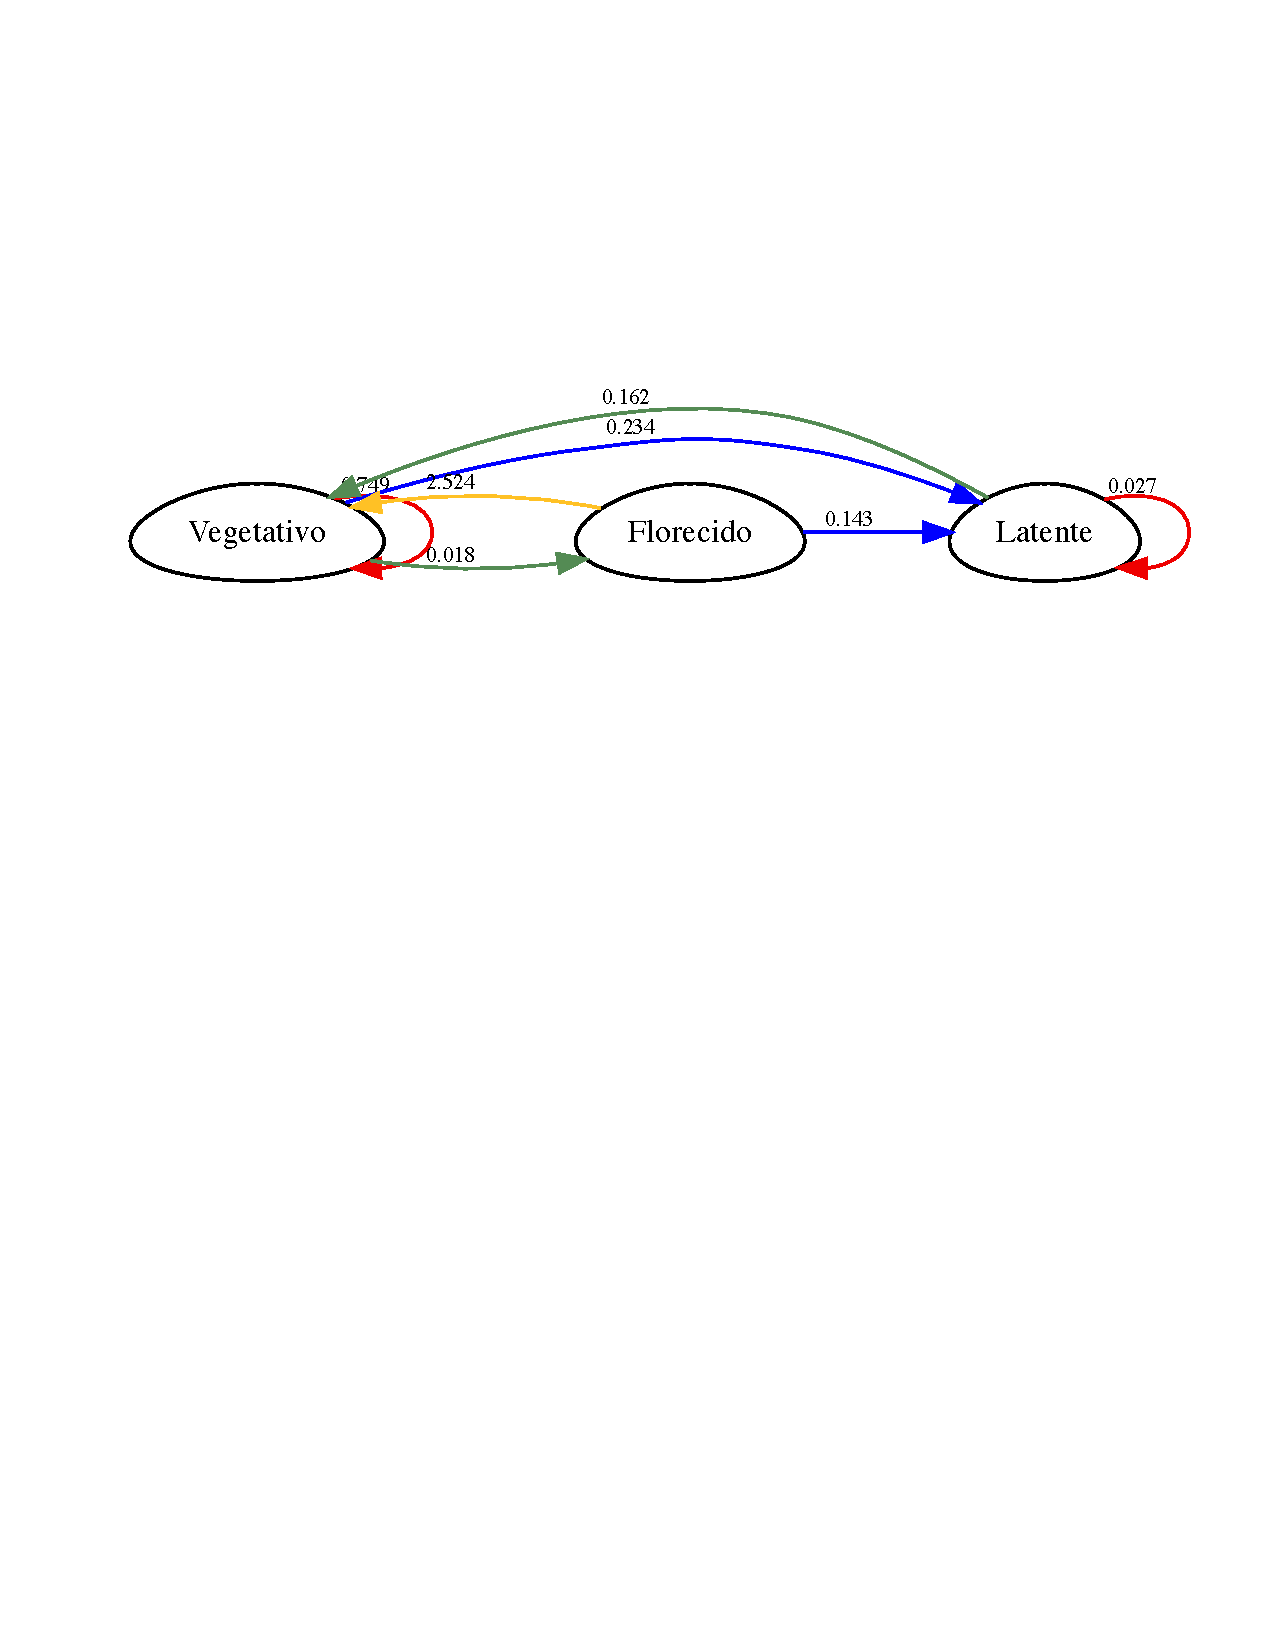
\includegraphics[keepaspectratio]{118-Carl_Olaf_Tamm_files/figure-pdf/OCTamm_11-1.pdf}}

\begin{center}\rule{0.5\linewidth}{0.5pt}\end{center}

\section{Análisis de viabilidad de
poblaciones}\label{anuxe1lisis-de-viabilidad-de-poblaciones}

Ahora usamos la información de las matrices de transiciones,
fertilidades y sus valores de prior para calcular los parámetros de la
especie

Antes de seguir, comparamos la matriz original con los valores de la
matriz posterior. Para calcular la matriz de transición y de fecundidad
posterior se usa la función ``priorweight'' para reducir o aumentar la
confianza que uno tiene sobre los valores prior. Nota que como estos
valores provienen de otra especies es buena idea reducir la confianza
que uno tiene sobre estos valores de ``priors'' en los análisis usando
un \textbf{priorweight} pequeño.

El valor de 0.01, es que se usa 1\% de los valores prior y 99\% de los
valores del campo. Por consecuencia dominará los valores del campo. Nota
que en la matriz posterior se observa valores en parámetros que
originalmente eran cero (ejemplo: plantas con flores que se queden con
flores, valores que no se observaron del campo). Nota ahora tenemos un
valor de 2\% de individuos que florecen en un año particular que se
quedan con flores en el año siguiente. Eso no fue un valor observado en
los datos de campo, pero es un valor que se puede calcular con los datos
que tenemos, y es probable que sea realista ya que ocurre en otras
especies de orquídeas del mismo género. Nota también que hay una pequeña
probabilidad que una planta latente sea fértil en el año siguiente
(0.004).

\begin{Shaded}
\begin{Highlighting}[]
\NormalTok{TF2}\SpecialCharTok{$}\NormalTok{Tmat}
\end{Highlighting}
\end{Shaded}

\begin{verbatim}
    stage
fate          V          F          D
   V 0.74853801 0.85714286 0.16216216
   F 0.01754386 0.00000000 0.00000000
   D 0.23391813 0.14285714 0.02702703
\end{verbatim}

\begin{Shaded}
\begin{Highlighting}[]
\NormalTok{TF3}\OtherTok{=}\FunctionTok{fill\_transitions}\NormalTok{(TF2, N2\_D, }\AttributeTok{P =}\NormalTok{ Dacty\_apriori, }\AttributeTok{priorweight =} \FloatTok{0.1}\NormalTok{)}

\NormalTok{TF3 }\CommentTok{\# la matriz de transiciones posterior}
\end{Highlighting}
\end{Shaded}

\begin{verbatim}
           [,1]       [,2]        [,3]
[1,] 0.73839819 0.83112987 0.214692875
[2,] 0.04076715 0.02463636 0.004454545
[3,] 0.22083466 0.14423377 0.029933661
\end{verbatim}

El estimado de \(\lambda\)

Como es esperado, la población de \emph{Dactylorhiza incarnata}
disminuye en el tiempo y el índice de crecimiento es menor que 1.0. El
valor de crecimiento intrínseco es de 0.84, lo que sugiere una
disminución de la población de aproximadamente 16\% por año. Era de
esperar que el crecimiento poblacional sea menor que 1.0, ya que la
mayoría de los individuos en la población son vegetativos y que la
mayoría de los individuos que florecen en un año particular no florecen
en el año siguiente, hay poco reclutamiento y el nivel de mortandad es
alta.

\begin{Shaded}
\begin{Highlighting}[]
\NormalTok{popbio}\SpecialCharTok{::}\FunctionTok{lambda}\NormalTok{(TF3)}
\end{Highlighting}
\end{Shaded}

\begin{verbatim}
[1] 0.8415307
\end{verbatim}

\section{Simulando el crecimiento
poblacional}\label{simulando-el-crecimiento-poblacional}

Uno de los retos en los análisis de viabilidad de población es la
construcción de intervalos de confianza. El valor anterior de lambda es
un valor puntual, pero no nos dice nada sobre la variabilidad de los
datos. Para calcular el intervalo de confianza se puede hacer una
simulación de Monte Carlo. En este caso se simula el crecimiento
poblacional de \emph{Dactylorhiza incarnata} muestreada por Tamm desde
1944 a 1971. Pero esta vez se usará información para hacer un modelo
completamente bayesiano. La ventaja es que los valores de credibilidad
de los parámetros son más informativos y se basan en la incertidumbre de
las transiciones.

Para estimar los intervalos de credibilidad se simula la matriz, tomando
en consideración el tamaño de muestra (N2\_d), las matrices de los
valores del campo (TF2), la matriz de los valores prior
(Dacty\_apriori), el peso de los valores prior (priorweight), los priors
de fertilidad y la cantidad de simulaciones (samples = 5000) que
queremos generar (para determinar la cantidad de simulaciones se puede
correr el análisis múltiples veces y evaluar si aumentar las
simulaciones impacta los intervalos de credibilidad). Con esta
simulación podemos calcular el intervalo de credibilidad del crecimiento
poblacional de \emph{Dactylorhiza incarnata} muestreada por Tamm desde
1944 a 1971.

Las matrices alpha2 y beta2, representan los parámetros de la
distribución gamma con media alpha/beta. En este caso se usa valores muy
pequeños para los valores alpha y beta, para que la distribución gamma
no sea informativa (non-informative priors) y que los valores de lambda
sean muy dispersos. En otras palabras no ponemos mucho peso en los
valores prior de la fertilidad, y dejamos que los valores del campo
dominen los análisis.

\begin{Shaded}
\begin{Highlighting}[]
\NormalTok{alpha2 }\OtherTok{\textless{}{-}} \FunctionTok{matrix}\NormalTok{(}\FunctionTok{c}\NormalTok{(}\ConstantTok{NA\_real\_}\NormalTok{, }\FloatTok{1e{-}5}\NormalTok{,     }\ConstantTok{NA\_real\_}\NormalTok{,}
                   \ConstantTok{NA\_real\_}\NormalTok{, }\ConstantTok{NA\_real\_}\NormalTok{, }\ConstantTok{NA\_real\_}\NormalTok{,}
                   \ConstantTok{NA\_real\_}\NormalTok{, }\ConstantTok{NA\_real\_}\NormalTok{, }\ConstantTok{NA\_real\_}\NormalTok{), }
          \AttributeTok{nrow=}\DecValTok{3}\NormalTok{, }\AttributeTok{ncol =} \DecValTok{3}\NormalTok{, }
          \AttributeTok{byrow =} \ConstantTok{TRUE}\NormalTok{) }\CommentTok{\# la matriz de los valores alpha}
\NormalTok{beta2 }\OtherTok{\textless{}{-}} \FunctionTok{matrix}\NormalTok{(}\FunctionTok{c}\NormalTok{( }\ConstantTok{NA\_real\_}\NormalTok{, }\FloatTok{1e{-}5}\NormalTok{,     }\ConstantTok{NA\_real\_}\NormalTok{,}
                   \ConstantTok{NA\_real\_}\NormalTok{, }\ConstantTok{NA\_real\_}\NormalTok{, }\ConstantTok{NA\_real\_}\NormalTok{,}
                   \ConstantTok{NA\_real\_}\NormalTok{, }\ConstantTok{NA\_real\_}\NormalTok{, }\ConstantTok{NA\_real\_}\NormalTok{), }
          \AttributeTok{nrow=}\DecValTok{3}\NormalTok{, }\AttributeTok{ncol =} \DecValTok{3}\NormalTok{, }
          \AttributeTok{byrow =} \ConstantTok{TRUE}\NormalTok{) }\CommentTok{\# la matriz de los valores beta}
\end{Highlighting}
\end{Shaded}

Ahora unimos todos los valores, para simular el crecimiento poblacional
de \emph{Dactylorhiza incarnata} con la función
\textbf{sim\_transitions} muestreado por Tamm desde 1944 a 1971.

\begin{itemize}
\tightlist
\item
  \textbf{TF2} es la matriz de transiciones y de fertilidades
\item
  \textbf{N2\_D} es el vector de la cantidad de individuos en cada etapa
\item
  \textbf{Dacty\_apriori} es la matriz de los valores prior
\item
  \textbf{alpha2} y \textbf{beta2} son los valores de los parámetros de
  la distribución gamma para la fertilidad
\item
  \textbf{priorweight} es el peso de los valores prior
\item
  \textbf{samples} es la cantidad de simulaciones que queremos generar.
\end{itemize}

\begin{Shaded}
\begin{Highlighting}[]
\NormalTok{Dacty\_0}\FloatTok{.1} \OtherTok{\textless{}{-}} \FunctionTok{sim\_transitions}\NormalTok{(}
\NormalTok{  TF2,}
\NormalTok{  N2\_D,}
  \AttributeTok{P =}\NormalTok{ Dacty\_apriori,}
  \AttributeTok{alpha =}\NormalTok{ alpha2,}
  \AttributeTok{beta =}\NormalTok{ beta2,}
  \AttributeTok{priorweight =} \FloatTok{0.1}\NormalTok{,}
  \AttributeTok{samples =} \DecValTok{5000}
\NormalTok{) }\CommentTok{\# generar 5000 matrices basado en las previas de transiciones y de fertilidades, el tamaño de muestra, en adición de los datos}
\end{Highlighting}
\end{Shaded}

Se convierte el objeto ``Dacty\_0.1'' en un tibble para poder visualizar
la distribución de los lambda que proviene de la simulación.

\begin{Shaded}
\begin{Highlighting}[]
\NormalTok{Dacty\_0}\FloatTok{.1}\NormalTok{b }\OtherTok{\textless{}{-}} \FunctionTok{tibble}\NormalTok{(}\AttributeTok{lposterior =} \FunctionTok{map\_dbl}\NormalTok{(Dacty\_0}\FloatTok{.1}\NormalTok{, lambda))}
\end{Highlighting}
\end{Shaded}

\section{Visualización de las distribuciones de los
lambda.}\label{visualizaciuxf3n-de-las-distribuciones-de-los-lambda.}

Se nota claramente que la población de \emph{Dactylorhiza incarnata}
muestreada por Tamm desde 1944 a 1971 tiene un crecimiento poblacional
menor que 1.0. Nota que esta simulación considera variación demográfica
en los datos.

\begin{Shaded}
\begin{Highlighting}[]
\FunctionTok{ggplot}\NormalTok{(}\AttributeTok{data =}\NormalTok{ Dacty\_0}\FloatTok{.1}\NormalTok{b, }\AttributeTok{mapping =} \FunctionTok{aes}\NormalTok{(}\AttributeTok{x =}\NormalTok{ lposterior)) }\SpecialCharTok{+}
  \FunctionTok{geom\_histogram}\NormalTok{(}\AttributeTok{binwidth =} \FloatTok{0.01}\NormalTok{, }\AttributeTok{colour =} \StringTok{"white"}\NormalTok{) }\SpecialCharTok{+}
  \FunctionTok{rlt\_style\_colour}\NormalTok{() }\SpecialCharTok{+}
  \FunctionTok{geom\_vline}\NormalTok{(}\AttributeTok{xintercept =} \DecValTok{1}\NormalTok{, }\AttributeTok{color =} \StringTok{"\#009392"}\NormalTok{, }\AttributeTok{size =} \FloatTok{1.5}\NormalTok{)}
\end{Highlighting}
\end{Shaded}

\pandocbounded{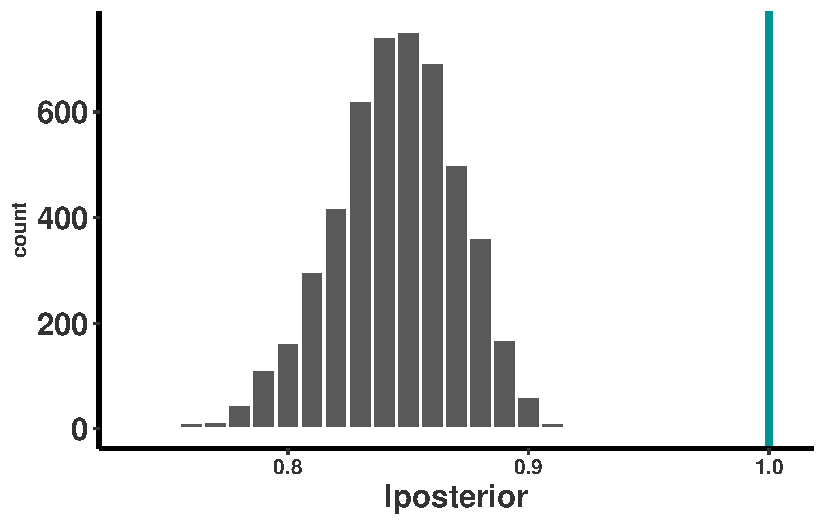
\includegraphics[keepaspectratio]{118-Carl_Olaf_Tamm_files/figure-pdf/OCTamm_17-1.pdf}}

Para concluir, la población de \emph{Dactylorhiza incarnata} muestreada
por Tamm desde 1944 a 1971 tiene un crecimiento poblacional menor que
1.0 (lambda promedio de 0.84), con un intervalo de credibilidad de 0.79
a 0.89. Esto indica que la población se está reduciendo en el tiempo por
aproximadamente 16\%, aunque la reducción real podría estar entre el
11\% y el 21\%. La columna \texttt{pincrease} reporta la probabilidad
posterior de que \(\lambda > 1\) (es decir, de que la población esté
creciendo). En este caso el valor es \textless0.001, lo que indica que
la población está decreciendo con muy alta certeza.

\begin{Shaded}
\begin{Highlighting}[]
\NormalTok{Dacty\_0}\FloatTok{.1}\NormalTok{bdf }\OtherTok{=} \FunctionTok{as.data.frame}\NormalTok{(Dacty\_0}\FloatTok{.1}\NormalTok{b)}
\NormalTok{Dacty\_0}\FloatTok{.1}\NormalTok{\_summary }\OtherTok{\textless{}{-}}\NormalTok{ dplyr}\SpecialCharTok{::}\FunctionTok{summarize}\NormalTok{(}
\NormalTok{  Dacty\_0}\FloatTok{.1}\NormalTok{bdf,}
  \AttributeTok{medianL =} \FunctionTok{median}\NormalTok{(lposterior),}
  \AttributeTok{meanL =} \FunctionTok{mean}\NormalTok{(lposterior),}
  \AttributeTok{lcl =} \FunctionTok{quantile}\NormalTok{(lposterior, }\AttributeTok{probs =} \FloatTok{0.025}\NormalTok{),}
  \AttributeTok{ucl =} \FunctionTok{quantile}\NormalTok{(lposterior, }\AttributeTok{probs =} \FloatTok{0.975}\NormalTok{),}
  \AttributeTok{pincrease =} \FunctionTok{sum}\NormalTok{(lposterior }\SpecialCharTok{\textgreater{}} \FloatTok{1.}\NormalTok{) }\SpecialCharTok{/} \FunctionTok{n}\NormalTok{()}
\NormalTok{)}
\end{Highlighting}
\end{Shaded}

\begin{Shaded}
\begin{Highlighting}[]
\FunctionTok{flextable}\NormalTok{(}\FunctionTok{signif}\NormalTok{(Dacty\_0}\FloatTok{.1}\NormalTok{\_summary, }\AttributeTok{digits =} \DecValTok{3}\NormalTok{))}
\end{Highlighting}
\end{Shaded}

\global\setlength{\Oldarrayrulewidth}{\arrayrulewidth}

\global\setlength{\Oldtabcolsep}{\tabcolsep}

\setlength{\tabcolsep}{2pt}

\renewcommand*{\arraystretch}{1.5}



\providecommand{\ascline}[3]{\noalign{\global\arrayrulewidth #1}\arrayrulecolor[HTML]{#2}\cline{#3}}

\begin{longtable*}[c]{ccccc}



\ascline{1.5pt}{666666}{1-5}

\multicolumn{1}{>{}r}{\textcolor[HTML]{000000}{\fontsize{11}{11}\selectfont{medianL}}} & \multicolumn{1}{>{}r}{\textcolor[HTML]{000000}{\fontsize{11}{11}\selectfont{meanL}}} & \multicolumn{1}{>{}r}{\textcolor[HTML]{000000}{\fontsize{11}{11}\selectfont{lcl}}} & \multicolumn{1}{>{}r}{\textcolor[HTML]{000000}{\fontsize{11}{11}\selectfont{ucl}}} & \multicolumn{1}{>{}r}{\textcolor[HTML]{000000}{\fontsize{11}{11}\selectfont{pincrease}}} \\

\ascline{1.5pt}{666666}{1-5}\endfirsthead 

\ascline{1.5pt}{666666}{1-5}

\multicolumn{1}{>{}r}{\textcolor[HTML]{000000}{\fontsize{11}{11}\selectfont{medianL}}} & \multicolumn{1}{>{}r}{\textcolor[HTML]{000000}{\fontsize{11}{11}\selectfont{meanL}}} & \multicolumn{1}{>{}r}{\textcolor[HTML]{000000}{\fontsize{11}{11}\selectfont{lcl}}} & \multicolumn{1}{>{}r}{\textcolor[HTML]{000000}{\fontsize{11}{11}\selectfont{ucl}}} & \multicolumn{1}{>{}r}{\textcolor[HTML]{000000}{\fontsize{11}{11}\selectfont{pincrease}}} \\

\ascline{1.5pt}{666666}{1-5}\endhead



\multicolumn{1}{>{}r}{\textcolor[HTML]{000000}{\fontsize{11}{11}\selectfont{0.845}}} & \multicolumn{1}{>{}r}{\textcolor[HTML]{000000}{\fontsize{11}{11}\selectfont{0.844}}} & \multicolumn{1}{>{}r}{\textcolor[HTML]{000000}{\fontsize{11}{11}\selectfont{0.79}}} & \multicolumn{1}{>{}r}{\textcolor[HTML]{000000}{\fontsize{11}{11}\selectfont{0.892}}} & \multicolumn{1}{>{}r}{\textcolor[HTML]{000000}{\fontsize{11}{11}\selectfont{0}}} \\

\ascline{1.5pt}{666666}{1-5}



\end{longtable*}



\arrayrulecolor[HTML]{000000}

\global\setlength{\arrayrulewidth}{\Oldarrayrulewidth}

\global\setlength{\tabcolsep}{\Oldtabcolsep}

\renewcommand*{\arraystretch}{1}

\part{Apéndices}

\chapter*{Apéndice A}\label{AppendixA}
\addcontentsline{toc}{chapter}{Apéndice A}

\markboth{Apéndice A}{Apéndice A}

\section*{Lista completa de MPP en
orquídeas}\label{lista-completa-de-mpp-en-orquuxeddeas}
\addcontentsline{toc}{section}{Lista completa de MPP en orquídeas}

\markright{Lista completa de MPP en orquídeas}

En esta sección se hace una recopilación de los estudios de dinámica
poblacional en orquídeas que han usado matrices de transición de estados
y de edades. Se identifican algunos de los temas principales de los
trabajos.

En la siguiente tabla se presentan los estudios de dinámica poblacional
en orquídeas que usaron MPP y las preguntas principales que los autores
intentaron responder. En la gran mayoría de los trabajos se evalúan
múltiples hipótesis/ideas sobre la dinámica poblacional de las
orquídeas. Para información específica sobre la metodología usada en
cada estudio, se recomienda revisar los trabajos originales.

\begin{itemize}
\item
  Clave de las variables:

  \begin{itemize}
  \tightlist
  \item
    \textbf{Riesgo}: Si se evaluó el riesgo de extinción de la especie.
  \item
    \textbf{Variación espacial}: Si se evaluó la variación espacial de
    la especie.
  \item
    \textbf{Variación temporal}: Si se evaluó la variación temporal de
    la especie.
  \item
    \textbf{Latencia}: Si se evaluó la importancia de la latencia
    (\emph{dormancy}) de la especie.
  \item
    \textbf{Métodos de estimación de parámetros}: Si se evaluaron
    métodos alternos de estimación de parámetros (no tradicionales).
  \item
    \textbf{Historia de vida}: Si se evaluó la historia de vida de la
    especie en un contexto evolutivo.
  \item
    \textbf{Otro}: Si se evaluó otra pregunta no incluida en las
    anteriores.
  \item
    \textbf{Referencia}: Referencia del estudio.
  \end{itemize}
\end{itemize}

\begin{Shaded}
\begin{Highlighting}[]
\FunctionTok{library}\NormalTok{(readr)}
\FunctionTok{library}\NormalTok{(tidyverse)}
\FunctionTok{library}\NormalTok{(dplyr)}
\FunctionTok{library}\NormalTok{(gt)}
\end{Highlighting}
\end{Shaded}

\begin{center}\rule{0.5\linewidth}{0.5pt}\end{center}

\begin{table}
\fontsize{9.0pt}{11.0pt}\selectfont
\begin{tabular*}{1\linewidth}{@{\extracolsep{\fill}}llllllllll}
\toprule
Género & Especies & Riesgo & Var. esp. & Var. temp. & Latencia & Est. param. & Hist. vida & Otro & Referencia \\ 
\midrule\addlinespace[2.5pt]
\emph{Aspasia} & \emph{principissa} & Si & - & Si & - & - & - & \begin{itemize}
\item 
\end{itemize} & @zotz2006population \\ 
\emph{Brassavola} & \emph{cucullata} & Si & Si & Si & - & - & - & IPM, Transient Dynamics, Transfer Function & @ackerman2020small \\ 
\emph{Broughtonia} & \emph{cubensis} & Si & Si & Si & - & - & - & Transient Dynamics & @raventos2021effects \\ 
\emph{Caladenia} & \emph{amoena} & Si & - & - & Si & Si & Si & Selección de modelos, método para estimar latencia & @tremblay2009population @tremblay2009dormancy; \\ 
\emph{Caladenia} & \emph{argocalla} & Si & - & - & Si & Si & Si & Selección de modelos, método para estimar latencia & @tremblay2009population @tremblay2009dormancy \\ 
\emph{Caladenia} & \emph{clavigera} & Si & - & - & Si & Si & Si & Selección de modelos, método para estimar latencia & @tremblay2009population  @tremblay2009dormancy \\ 
\emph{Caladenia} & \emph{elegans} & Si & - & - & Si & Si & Si & Selección de modelos, método para estimar latencia & @tremblay2009population @tremblay2009dormancy \\ 
\emph{Caladenia} & \emph{graniticola} & Si & - & - & Si & Si & Si & Selección de modelos, método para estimar latencia & @tremblay2009population @tremblay2009dormancy \\ 
\emph{Caladenia} & \emph{macroclavia} & Si & - & - & Si & Si & Si & Selección de modelos, método para estimar latencia & @tremblay2009population @tremblay2009dormancy \\ 
\emph{Caladenia} & \emph{oenochila} & Si & - & - & Si & Si & Si & Selección de modelos, método para estimar latencia & @tremblay2009population @tremblay2009dormancy \\ 
\emph{Caladenia} & \emph{rosella} & Si & - & - & Si & Si & Si & Selección de modelos, método para estimar latencia & @tremblay2009population @tremblay2009dormancy \\ 
\emph{Caladenia} & \emph{valida} & Si & - & - & Si & Si & Si & Selección de modelos, método para estimar latencia & @tremblay2009population @tremblay2009dormancy \\ 
\emph{Caladenia} & \emph{orientalis} & Si & Si & Si & Si & - & - & Interacciones abióticas & @coates2009demographic \\ 
\emph{Cephalanthera} & \emph{longifolia} & - & - & - & Si & Si & Si & Interacciones abióticas y bióticas & @shefferson2012linking \\ 
\emph{Cleistes} & \emph{divaricata} var. \emph{divaricata} & Si & Si & Si & Si & Si & - & \begin{itemize}
\item 
\end{itemize} & @gregg1991variation \\ 
\emph{Cleistes} & \emph{divaricata} var. \emph{bifaria} & Si & Si & Si & Si & Si & - & \begin{itemize}
\item 
\end{itemize} & @gregg1991variation \\ 
\emph{Cleistes} & \emph{bifaria} & - & Si & - & Si & - & - & Estructura de tamaño y estado & @gregg2006comparison \\ 
\emph{Corallorhiza} & \emph{trifida} & Si & - & Si & Si & - & - & \begin{itemize}
\item 
\end{itemize} & @iriondo2009peligro \\ 
\emph{Crepidium} & \emph{acuminatum} & Si & - & Si & - & - & - & Efecto de cosecha & @timsina2021six \\ 
\emph{Cypripedium} & \emph{acaule} & - & - & - & - & Si & - & Edad de individuos reproductivos & @cochran1992simple \\ 
\emph{Cypripedium} & \emph{calceolus} & Si & Si & Si & Si & - & - & Selección de modelos & @nicole2005population \\ 
\emph{Cypripedium} & \emph{calceolus} & Si & Si & Si & Si & - & - & Efecto de aislamiento & @garcia2010living \\ 
\emph{Cypripedium} & \emph{calceolus} & - & - & - & - & - & - & Costo de latencia, Interacciones abióticas y bióticas & @shefferson2012linking \\ 
\emph{Cypripedium} & \emph{fasciculatum} & Si & Si & Si & Si & - & - & Selección de modelos, Interacciones abióticas & @thorpe2011trends \\ 
\emph{Cypripedium} & \emph{parviflorum} & - & - & - & Si & - & Si & \begin{itemize}
\item 
\end{itemize} & @shefferson2014life \\ 
\emph{Cypripedium} & \emph{reginae} & - & Si & - & Si & - & Si & Selección de modelos, interacciones bióticas & @kery2004demographic \\ 
\emph{Cypripedium} & \emph{lentiginosum} & - & - & - & - & Si & - & Leslie matrix & @zhongjian2008correlation \\ 
\emph{Dactylorhiza} & \emph{hatagirea} & Si & Si & Si & Si & - & - & Efecto de cosecha & @chapagain2021illegal \\ 
\emph{Dactylorhiza} & \emph{lapponica} & - & Si & Si & Si & - & - & Efecto antropogénico, interacciones abióticas & @sletvold2010long; @sletvold2013climate \\ 
\emph{Dendrophylax} & \emph{lindenii} & Si & - & Si & - & - & - & Efecto de densidad, \textbf{los datos de la matriz no están disponibles} & @gonzalez2009dinamica; @raventos2015population \\ 
\emph{Epidendrum} & \emph{xanthinum} & Si & Si & - & - & - & - & Comparación de poblaciones & @farfan2008estrategias \\ 
\emph{Epipactis} & \emph{atrorubens} & Si & Si & Si & Si  & - & - & Incorporación de variable de endogamia & @hens2017low \\ 
\emph{Epipactis} & \emph{atrorubens} & - & - & - & -  & - & - &  & @jakalaniemi2011orchids \\ 
\emph{Erycina} & \emph{crista-galli} & Si & Si & - & - & - & - & \begin{itemize}
\item 
\end{itemize} & @mondragon2007life \\ 
\emph{Erycina} & \emph{crista-galli} & - & - & - & - & - & - & \begin{itemize}
\item 
\end{itemize} & @maldonado2005patron \\ 
\emph{Guarianthe} & \emph{aurantiaca} & Si & Si & - & - & - & - & Efecto de cosecha & @mondragon2009population \\ 
\emph{Herminium} & \emph{monorchis} & Si & - & Si & Si & - & - & Efecto abiótico & @wells1998flowering \\ 
\emph{Himantoglossum} & \emph{hircinum} & Si & - & Si & - & - & - & Efecto abiótico: sequía & @wells1998flowering \\ 
\emph{Himantoglossum} & \emph{hircinum} & Si & - & Si & - & - & - & Modelando expansión & @carey1998modelling \\ 
\emph{Himantoglossum} & \emph{hircinum} & Si & - & Si & Si & - & - & Efecto abiótico: Precipitación y Temp del suelo & @pfeifer2006influence \\ 
\emph{Isotria} & \emph{medeoloides} & Si & - & Si & - & - & - & Tratamiento del dosel & @dibble2019demography \\ 
\emph{Jacquiniella} & \emph{leucomelana} & Si & - & Si & - & - & - & Metapopulation approach & @winkler2009population \\ 
\emph{Jacquiniella} & \emph{teretifolia} & Si & - & Si & - & - & - & Metapopulation approach & @winkler2009population \\ 
\emph{Laelia} & \emph{autumnalis} & Si & Si & Si & - & - &  & Efecto de cosecha & @emeterio2021does \\ 
\emph{Laelia} & \emph{speciosa} & Si & - & Si & - & - & - & Efecto de cosecha & @hernandez1992dinamica \\ 
\emph{Lepanthes} & \emph{caritensis} & Si & Si & Si & - & - & - & \begin{itemize}
\item 
\end{itemize} & @tremblay1997lepanthes \\ 
\emph{Lepanthes} & \emph{caritensis} & Si & Si & Si & - & - & - & Efecto de huracanes & @crain2019sheltered \\ 
\emph{Lepanthes} & \emph{eltoroensis} & Si & Si & - & - & - & - & Tamaño efectivo de Población, Ne y largo de vida & @tremblay2001gene \\ 
\emph{Lepanthes} & \emph{eltoroensis} & Si & Si & Si & - & - & - & \begin{itemize}
\item 
\end{itemize} & @tremblay2003population \\ 
\emph{Lepanthes} & \emph{eltoroensis} & Si & Si & Si & Si & - & - & Nueva metodología para estimar parámetros & @tremblay2021population \\ 
\emph{Lepanthes} & \emph{rubripetala} & - & - & - & - & - & - & Tamaño efectivo de Población, Ne y largo de vida & @tremblay2001gene \\ 
\emph{Lepanthes} & \emph{rubripetala} & Si & Si & Si & - & - & - & Dinámica de transiciones & @tremblay2015stable \\ 
\emph{Lepanthes} & \emph{rupestris} & - & - & - & - & - & - & Tamaño efectivo de Población, Ne y largo de vida & @tremblay2001gene \\ 
\emph{Lepanthes} & \emph{acuminata} & Si & - & - & - & - & - & Dinámica de transiciones & @raventos2018comparison \\ 
\emph{Lycaste} & \emph{aromatica} & Si & - & Si & - & - & - & Metapopulation approach & @winkler2009population \\ 
\emph{Neotinea} & \emph{ustulata} & Si & Si & - & Si & - & Si & Método para estimar latencia & @shefferson2007dormancy \\ 
\emph{Oeceoclades} & \emph{maculata} & Si & Si & Si & - & - & - & Especie invasiva & @riveron2019spatio \\ 
\emph{Oncidium} & \emph{poikilostalix} & Si & - & - & - & - & - & Dinámica de transiciones & @raventos2018comparison \\ 
\emph{Orchis} & \emph{purpurea} & Si & - & Si & - & - & - & LTRE & @jacquemyn2010seed \\ 
\emph{Orchis} & \emph{ustulata} & Si & Si & - & - & - & - & mismo que \emph{Neotinea ustulata} & @tali2002dynamics \\ 
\emph{Phaius} & \emph{australis} & Si & Si & - & - & - & - & Efecto espacial y abiótico & @simmons2016Viability \\ 
\emph{Platanthera} & \emph{hookeri} & Si & Si & - & - & - & - & \begin{itemize}
\item 
\end{itemize} & @reddoch2007population \\ 
\emph{Platanthera} & \emph{praeclara} & Si & Si & Si & Si & - & - & Variación temporal & @sieg1995influence \\ 
\emph{Platanthera} & \emph{macrophylla} & Si & Si & Si & - & - & - & Incluye estado de protocormo & @cleavitt2017life @berry2021population \\ 
\emph{Platanthera} & \emph{orbiculata} & Si & Si & Si & - & - & - & Incluye estado de protocormo & @cleavitt2017life @berry2021population \\ 
\emph{Prasophyllum} & \emph{correctum} & Si &  & Si & Si & - & - & Efecto de fuego & @coates2006effects \\ 
\emph{Pseudorchis} & \emph{albida} & - & - & - & - & - & - & \begin{itemize}
\item 
\end{itemize} & @stipkova2013mowing \\ 
\emph{Rodriguezia} & \emph{granadensis} & Si & Si & Si & - & - &  & Efecto antropogénico, \textbf{to be digitized} & @ospina2023effect \\ 
\emph{Serapias} & \emph{cordigera} & Si & Si & Si & Si & - & - & Efecto antropogénico & @pellegrino2014effects \\ 
\emph{Spathoglottis} & \emph{plicata} & Si & Si & Si & - & - & - & Orquídea invasiva y interacciones bióticas & @falcon2017quantifying \\ 
\emph{Spiranthes} & \emph{delitescens} & Si & Si & Si & Si & - & - & Efecto abiótico: sequía & @mcclaran1992population \\ 
\emph{Spiranthes} & \emph{parksii} & Si &  & - & - & - & - & Efecto abiótico: herbivoría & @wonka2010herbivores \\ 
\emph{Telipogon} & \emph{helleri} & Si & - & - & - & - & Si & Dinámica de transición & @raventos2018comparison \\ 
\emph{Tolumnia} & \emph{variegata} & Si & Si & Si & - & - & Si & El costo de reproducción & @calvo1993evolutionary \\ 
\emph{Trichocentrum} & \emph{undulatum} & - & - & - & - & - &  & Efecto de aislamiento & @borrero2023populations \\ 
\bottomrule
\end{tabular*}
\end{table}

\begin{figure}[H]

{\centering \pandocbounded{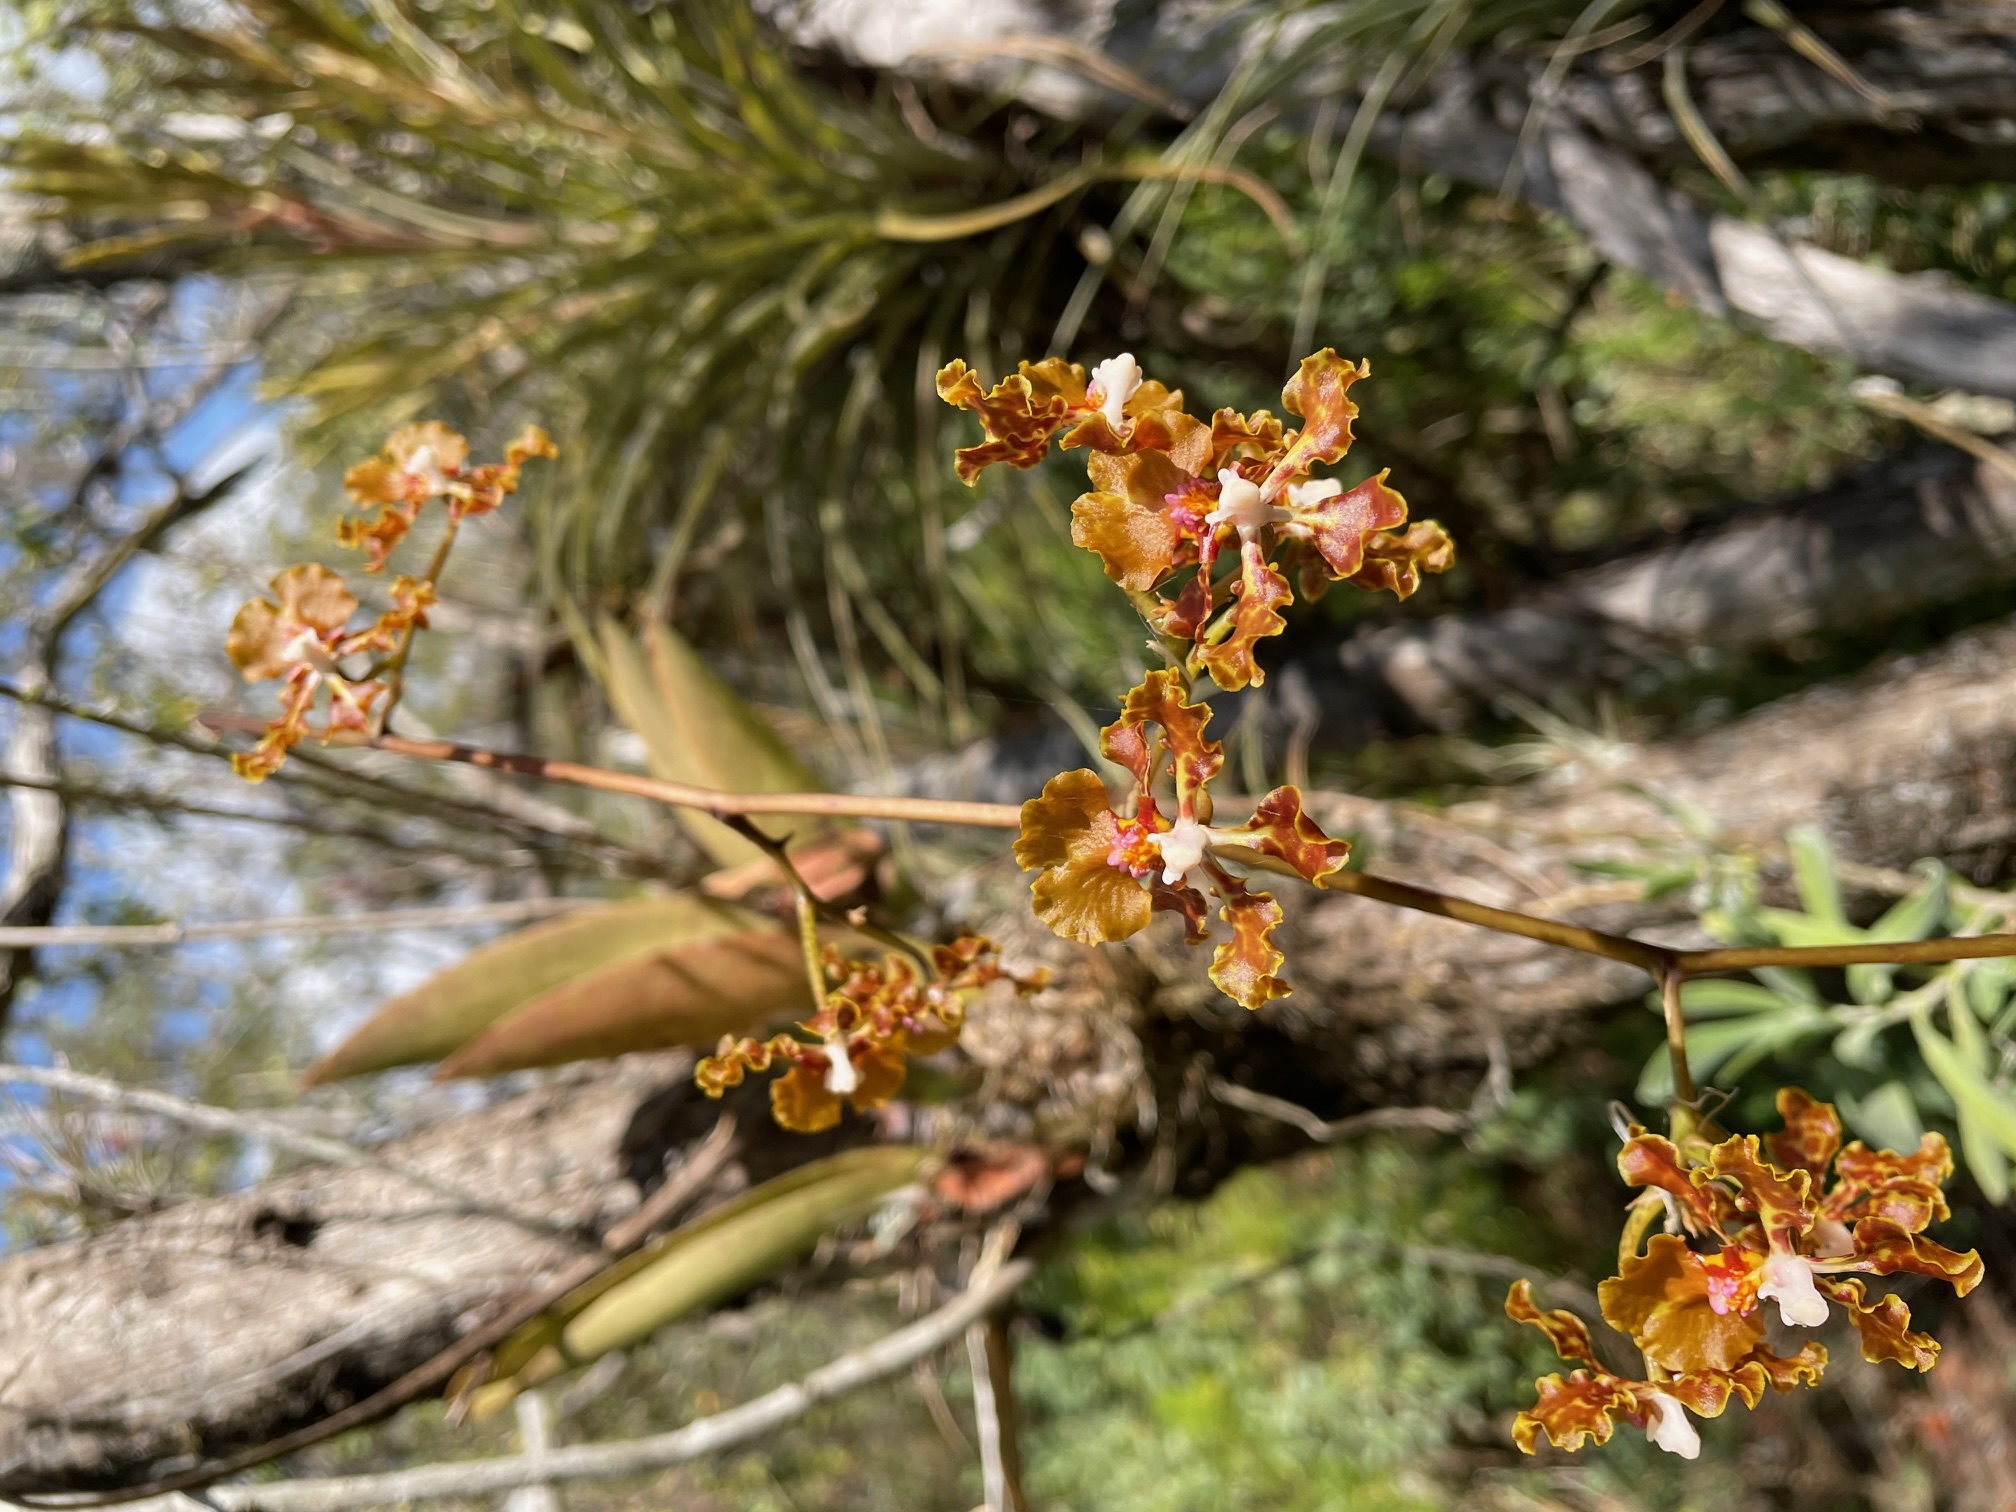
\includegraphics[keepaspectratio]{images/Trichocentrum_undulatum_8_Hong_Liu.jpg}}

}

\caption{\emph{Trichocentrum undulatum}. Foto: Hong Liu}

\end{figure}%

\begin{center}\rule{0.5\linewidth}{0.5pt}\end{center}

Notas para añadir a la tabla

\begin{itemize}
\tightlist
\item
  IPM - Integrated Population Model
\item
  Transient dynamics
\item
  Transfer function
\end{itemize}

\begin{center}\rule{0.5\linewidth}{0.5pt}\end{center}

\section*{Especies de orquídeas estudiadas sin
MPP}\label{especies-de-orquuxeddeas-estudiadas-sin-mpp}
\addcontentsline{toc}{section}{Especies de orquídeas estudiadas sin MPP}

\markright{Especies de orquídeas estudiadas sin MPP}

En la siguiente lista incluimos algunos de los trabajos de dinámica
poblacional que no usan MPP para responder a su pregunta. La lista es
muy grande y no es exhaustiva. Incluye trabajos que usan otros métodos
de estimación de parámetros, como modelos de regresión, o que usan IPM
(\emph{Integral Population Models}), pero no usan matrices de transición
de estados o edades, que es el método alterno de estimación de
parámetros que se usa en este libro.

\begin{figure}[H]

{\centering \pandocbounded{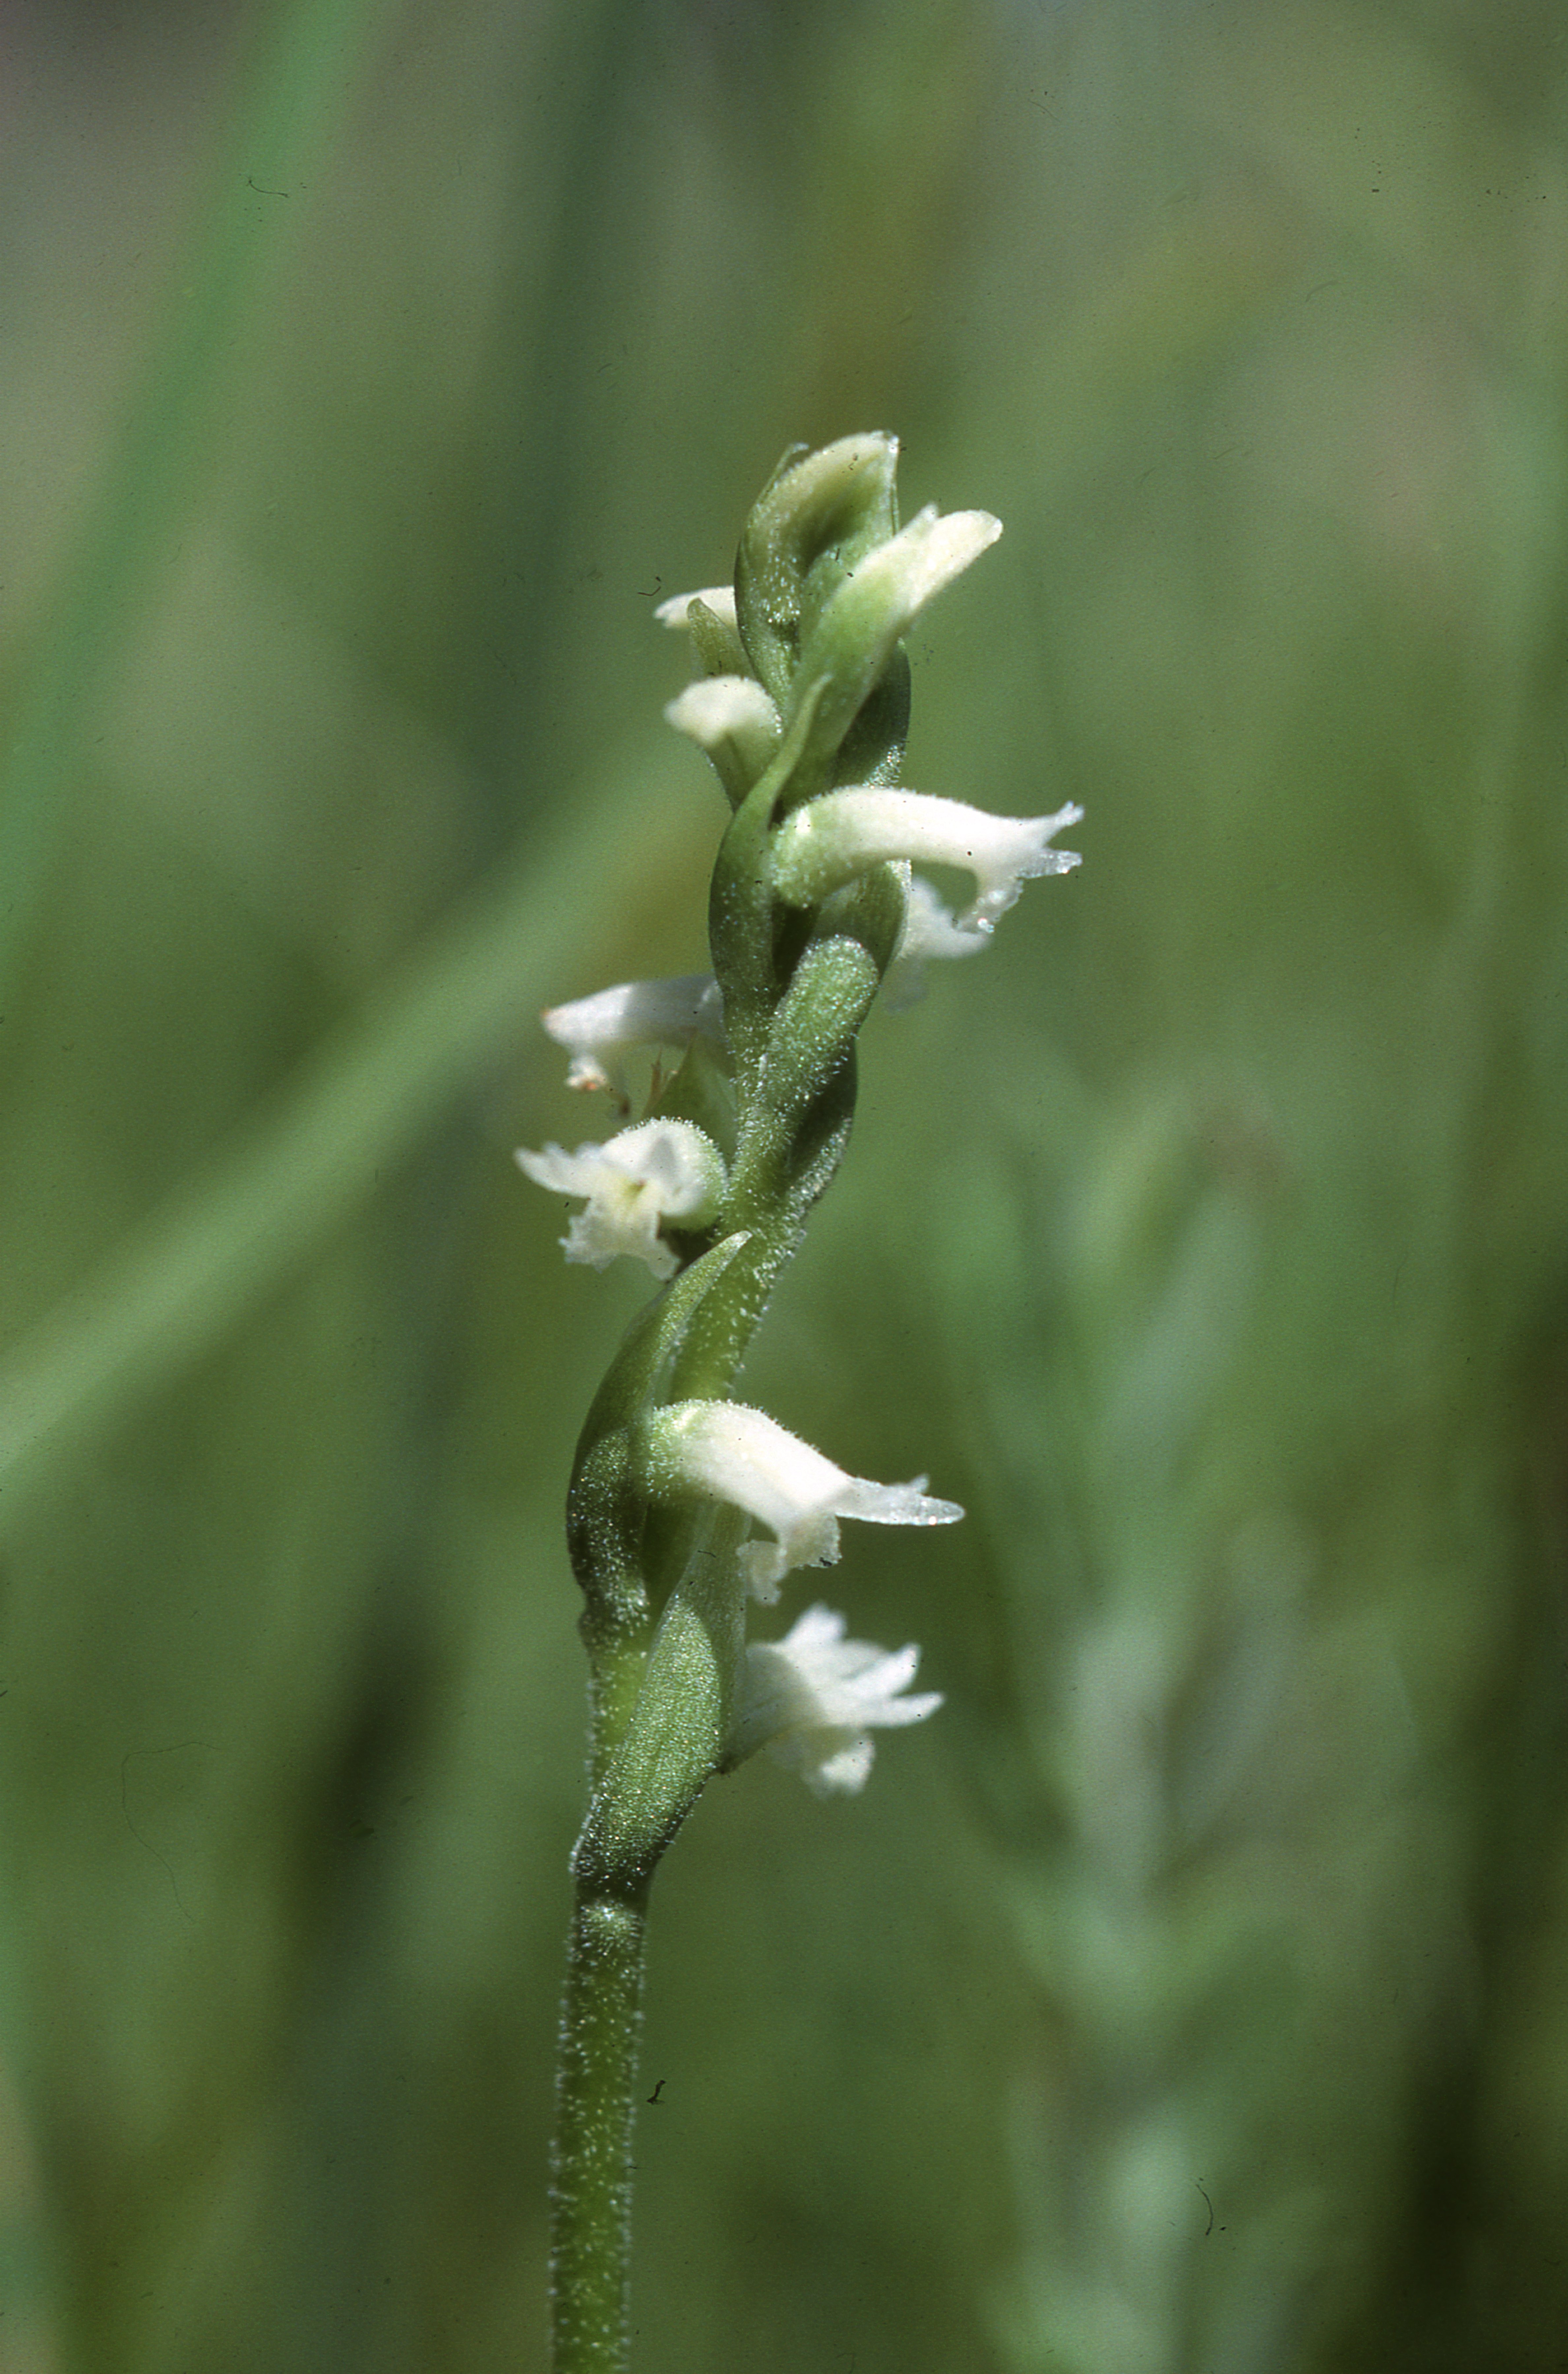
\includegraphics[keepaspectratio]{images/Spiranthes_delitescens_Mitchel_Mcclaran.jpg}}

}

\caption{\emph{Spiranthes delitescens}. Foto: Mitchel McClaran}

\end{figure}%

\begin{table}
\fontsize{9.0pt}{11.0pt}\selectfont
\begin{tabular*}{1\linewidth}{@{\extracolsep{\fill}}llll}
\toprule
Género & Especies & Otro & Referencia \\ 
\midrule\addlinespace[2.5pt]
\emph{Isotria} & \emph{medeoloides} & no matrix & @alahuhta2017instant \\ 
\emph{Cyclopogon} & \emph{luteoalbus} & no matrix & @juarez2014viability \\ 
\emph{Cypripedium} & \emph{calceolus} & no matrix & @davison2013contributions \\ 
\emph{Cypripedium} & \emph{candidum} & no matrix & @shefferson2017predicting \\ 
\emph{Gymnadenia} & \emph{conopsea} & no matrix & @oien2002flowering \\ 
\emph{Ophrys} & \emph{sphegodes} & no matrix & @hutchings2010population \\ 
\emph{Ophrys} & \emph{sphegodes} & no matrix & @shefferson2017predicting \\ 
\emph{Orchis} & \emph{morio} & no matrix & @wells1998flowering \\ 
\emph{Spiranthes} & \emph{spiralis} & no matrix & @jacquemyn2007long \\ 
\bottomrule
\end{tabular*}
\end{table}

\chapter*{Apéndice B}\label{apuxe9ndice-b}
\addcontentsline{toc}{chapter}{Apéndice B}

\markboth{Apéndice B}{Apéndice B}

\section*{Hojas de datos en el campo}\label{hojas-de-datos-en-el-campo}
\addcontentsline{toc}{section}{Hojas de datos en el campo}

\markright{Hojas de datos en el campo}

Por: Raymond L. Tremblay

\subsubsection*{Librerías de R requeridas para el siguiente
módulo}\label{libreruxedas-de-r-requeridas-para-el-siguiente-muxf3dulo-19}
\addcontentsline{toc}{subsubsection}{Librerías de R requeridas para el
siguiente módulo}

\begin{Shaded}
\begin{Highlighting}[]
\FunctionTok{library}\NormalTok{(tidyverse)}
\FunctionTok{library}\NormalTok{(flextable)}
\end{Highlighting}
\end{Shaded}

Presentamos un ejemplo de hoja de recolección de datos con algunas
variables incluidas, que debería estar preparada antes de ir al campo, e
impresa sobre papel impermeable que se pueda escribir con lápiz. Estos
últimos puntos son muy importantes, ya que la gran mayoría de los
bolígrafos son solubles en agua y, si el papel se moja, se pueden perder
los datos. Considerando que estas hojas de datos pudiesen ser usadas
como fuente para consultar los datos décadas en el futuro:
\textbf{recuerda que no se puede regresar con una máquina del tiempo
para recoger los datos}. Si tienes tu hoja de datos en el laboratorio y
se te cae la taza de café, y los datos fueron escritos con bolígrafo, se
pueden perder. ¡No se arriesgue! \textbf{Usa lápiz}.

Antes de ir al campo es importante tener la lista completa de todos los
individuos en la hoja de datos, ya que esto ayuda a asegurarse durante
el muestreo de que no se olvide ningún individuo. \emph{Datos olvidados
no se pueden recuperar}.

Puede usar papel \emph{Rite in the Rain} o papel de impresora normal. Si
usa papel normal, se puede poner en una bolsa de plástico con un pedazo
de cartón para que no se doble. Si se moja, se puede secar y no se
pierden los datos. Mi sugerencia: use papel \textbf{Rite in the Rain} y
lápiz.

\section*{Ejemplo de Hojas de campo}\label{ejemplo-de-hojas-de-campo}
\addcontentsline{toc}{section}{Ejemplo de Hojas de campo}

\markright{Ejemplo de Hojas de campo}

Hoja en blanco para llevarse

\begin{Shaded}
\begin{Highlighting}[]
\NormalTok{Hoja\_de\_campo }\SpecialCharTok{\%\textgreater{}\%} \FunctionTok{flextable}\NormalTok{()}
\end{Highlighting}
\end{Shaded}

\global\setlength{\Oldarrayrulewidth}{\arrayrulewidth}

\global\setlength{\Oldtabcolsep}{\tabcolsep}

\setlength{\tabcolsep}{2pt}

\renewcommand*{\arraystretch}{1.5}



\providecommand{\ascline}[3]{\noalign{\global\arrayrulewidth #1}\arrayrulecolor[HTML]{#2}\cline{#3}}

\begin{longtable*}[c]{ccccccccc}



\ascline{1.5pt}{666666}{1-9}

\multicolumn{1}{>{}r}{\textcolor[HTML]{000000}{\fontsize{11}{11}\selectfont{anio}}} & \multicolumn{1}{>{}r}{\textcolor[HTML]{000000}{\fontsize{11}{11}\selectfont{Número\_de\_Ind}}} & \multicolumn{1}{>{}l}{\textcolor[HTML]{000000}{\fontsize{11}{11}\selectfont{Etapa}}} & \multicolumn{1}{>{}l}{\textcolor[HTML]{000000}{\fontsize{11}{11}\selectfont{Cantidad\_flores\_abierta}}} & \multicolumn{1}{>{}l}{\textcolor[HTML]{000000}{\fontsize{11}{11}\selectfont{Cantidad\_capullo}}} & \multicolumn{1}{>{}l}{\textcolor[HTML]{000000}{\fontsize{11}{11}\selectfont{Cantidad\_Frutos}}} & \multicolumn{1}{>{}l}{\textcolor[HTML]{000000}{\fontsize{11}{11}\selectfont{Numero\_Hojas}}} & \multicolumn{1}{>{}l}{\textcolor[HTML]{000000}{\fontsize{11}{11}\selectfont{Ancho\_hoja\_mm}}} & \multicolumn{1}{>{}l}{\textcolor[HTML]{000000}{\fontsize{11}{11}\selectfont{etc}}} \\

\ascline{1.5pt}{666666}{1-9}\endfirsthead 

\ascline{1.5pt}{666666}{1-9}

\multicolumn{1}{>{}r}{\textcolor[HTML]{000000}{\fontsize{11}{11}\selectfont{anio}}} & \multicolumn{1}{>{}r}{\textcolor[HTML]{000000}{\fontsize{11}{11}\selectfont{Número\_de\_Ind}}} & \multicolumn{1}{>{}l}{\textcolor[HTML]{000000}{\fontsize{11}{11}\selectfont{Etapa}}} & \multicolumn{1}{>{}l}{\textcolor[HTML]{000000}{\fontsize{11}{11}\selectfont{Cantidad\_flores\_abierta}}} & \multicolumn{1}{>{}l}{\textcolor[HTML]{000000}{\fontsize{11}{11}\selectfont{Cantidad\_capullo}}} & \multicolumn{1}{>{}l}{\textcolor[HTML]{000000}{\fontsize{11}{11}\selectfont{Cantidad\_Frutos}}} & \multicolumn{1}{>{}l}{\textcolor[HTML]{000000}{\fontsize{11}{11}\selectfont{Numero\_Hojas}}} & \multicolumn{1}{>{}l}{\textcolor[HTML]{000000}{\fontsize{11}{11}\selectfont{Ancho\_hoja\_mm}}} & \multicolumn{1}{>{}l}{\textcolor[HTML]{000000}{\fontsize{11}{11}\selectfont{etc}}} \\

\ascline{1.5pt}{666666}{1-9}\endhead



\multicolumn{1}{>{}r}{\textcolor[HTML]{000000}{\fontsize{11}{11}\selectfont{2,023}}} & \multicolumn{1}{>{}r}{\textcolor[HTML]{000000}{\fontsize{11}{11}\selectfont{23,001}}} & \multicolumn{1}{>{}l}{\textcolor[HTML]{000000}{\fontsize{11}{11}\selectfont{...}}} & \multicolumn{1}{>{}l}{\textcolor[HTML]{000000}{\fontsize{11}{11}\selectfont{...}}} & \multicolumn{1}{>{}l}{\textcolor[HTML]{000000}{\fontsize{11}{11}\selectfont{...}}} & \multicolumn{1}{>{}l}{\textcolor[HTML]{000000}{\fontsize{11}{11}\selectfont{...}}} & \multicolumn{1}{>{}l}{\textcolor[HTML]{000000}{\fontsize{11}{11}\selectfont{...}}} & \multicolumn{1}{>{}l}{\textcolor[HTML]{000000}{\fontsize{11}{11}\selectfont{...}}} & \multicolumn{1}{>{}l}{\textcolor[HTML]{000000}{\fontsize{11}{11}\selectfont{...}}} \\





\multicolumn{1}{>{}r}{\textcolor[HTML]{000000}{\fontsize{11}{11}\selectfont{2,023}}} & \multicolumn{1}{>{}r}{\textcolor[HTML]{000000}{\fontsize{11}{11}\selectfont{23,002}}} & \multicolumn{1}{>{}l}{\textcolor[HTML]{000000}{\fontsize{11}{11}\selectfont{...}}} & \multicolumn{1}{>{}l}{\textcolor[HTML]{000000}{\fontsize{11}{11}\selectfont{...}}} & \multicolumn{1}{>{}l}{\textcolor[HTML]{000000}{\fontsize{11}{11}\selectfont{...}}} & \multicolumn{1}{>{}l}{\textcolor[HTML]{000000}{\fontsize{11}{11}\selectfont{...}}} & \multicolumn{1}{>{}l}{\textcolor[HTML]{000000}{\fontsize{11}{11}\selectfont{...}}} & \multicolumn{1}{>{}l}{\textcolor[HTML]{000000}{\fontsize{11}{11}\selectfont{...}}} & \multicolumn{1}{>{}l}{\textcolor[HTML]{000000}{\fontsize{11}{11}\selectfont{...}}} \\





\multicolumn{1}{>{}r}{\textcolor[HTML]{000000}{\fontsize{11}{11}\selectfont{2,023}}} & \multicolumn{1}{>{}r}{\textcolor[HTML]{000000}{\fontsize{11}{11}\selectfont{23,003}}} & \multicolumn{1}{>{}l}{\textcolor[HTML]{000000}{\fontsize{11}{11}\selectfont{...}}} & \multicolumn{1}{>{}l}{\textcolor[HTML]{000000}{\fontsize{11}{11}\selectfont{...}}} & \multicolumn{1}{>{}l}{\textcolor[HTML]{000000}{\fontsize{11}{11}\selectfont{...}}} & \multicolumn{1}{>{}l}{\textcolor[HTML]{000000}{\fontsize{11}{11}\selectfont{...}}} & \multicolumn{1}{>{}l}{\textcolor[HTML]{000000}{\fontsize{11}{11}\selectfont{...}}} & \multicolumn{1}{>{}l}{\textcolor[HTML]{000000}{\fontsize{11}{11}\selectfont{...}}} & \multicolumn{1}{>{}l}{\textcolor[HTML]{000000}{\fontsize{11}{11}\selectfont{...}}} \\





\multicolumn{1}{>{}r}{\textcolor[HTML]{000000}{\fontsize{11}{11}\selectfont{2,024}}} & \multicolumn{1}{>{}r}{\textcolor[HTML]{000000}{\fontsize{11}{11}\selectfont{23,001}}} & \multicolumn{1}{>{}l}{\textcolor[HTML]{000000}{\fontsize{11}{11}\selectfont{...}}} & \multicolumn{1}{>{}l}{\textcolor[HTML]{000000}{\fontsize{11}{11}\selectfont{...}}} & \multicolumn{1}{>{}l}{\textcolor[HTML]{000000}{\fontsize{11}{11}\selectfont{...}}} & \multicolumn{1}{>{}l}{\textcolor[HTML]{000000}{\fontsize{11}{11}\selectfont{...}}} & \multicolumn{1}{>{}l}{\textcolor[HTML]{000000}{\fontsize{11}{11}\selectfont{...}}} & \multicolumn{1}{>{}l}{\textcolor[HTML]{000000}{\fontsize{11}{11}\selectfont{...}}} & \multicolumn{1}{>{}l}{\textcolor[HTML]{000000}{\fontsize{11}{11}\selectfont{...}}} \\





\multicolumn{1}{>{}r}{\textcolor[HTML]{000000}{\fontsize{11}{11}\selectfont{2,024}}} & \multicolumn{1}{>{}r}{\textcolor[HTML]{000000}{\fontsize{11}{11}\selectfont{23,002}}} & \multicolumn{1}{>{}l}{\textcolor[HTML]{000000}{\fontsize{11}{11}\selectfont{...}}} & \multicolumn{1}{>{}l}{\textcolor[HTML]{000000}{\fontsize{11}{11}\selectfont{...}}} & \multicolumn{1}{>{}l}{\textcolor[HTML]{000000}{\fontsize{11}{11}\selectfont{...}}} & \multicolumn{1}{>{}l}{\textcolor[HTML]{000000}{\fontsize{11}{11}\selectfont{...}}} & \multicolumn{1}{>{}l}{\textcolor[HTML]{000000}{\fontsize{11}{11}\selectfont{...}}} & \multicolumn{1}{>{}l}{\textcolor[HTML]{000000}{\fontsize{11}{11}\selectfont{...}}} & \multicolumn{1}{>{}l}{\textcolor[HTML]{000000}{\fontsize{11}{11}\selectfont{...}}} \\





\multicolumn{1}{>{}r}{\textcolor[HTML]{000000}{\fontsize{11}{11}\selectfont{2,024}}} & \multicolumn{1}{>{}r}{\textcolor[HTML]{000000}{\fontsize{11}{11}\selectfont{24,003}}} & \multicolumn{1}{>{}l}{\textcolor[HTML]{000000}{\fontsize{11}{11}\selectfont{...}}} & \multicolumn{1}{>{}l}{\textcolor[HTML]{000000}{\fontsize{11}{11}\selectfont{...}}} & \multicolumn{1}{>{}l}{\textcolor[HTML]{000000}{\fontsize{11}{11}\selectfont{...}}} & \multicolumn{1}{>{}l}{\textcolor[HTML]{000000}{\fontsize{11}{11}\selectfont{...}}} & \multicolumn{1}{>{}l}{\textcolor[HTML]{000000}{\fontsize{11}{11}\selectfont{...}}} & \multicolumn{1}{>{}l}{\textcolor[HTML]{000000}{\fontsize{11}{11}\selectfont{...}}} & \multicolumn{1}{>{}l}{\textcolor[HTML]{000000}{\fontsize{11}{11}\selectfont{...}}} \\





\multicolumn{1}{>{}r}{\textcolor[HTML]{000000}{\fontsize{11}{11}\selectfont{2,024}}} & \multicolumn{1}{>{}r}{\textcolor[HTML]{000000}{\fontsize{11}{11}\selectfont{24,004}}} & \multicolumn{1}{>{}l}{\textcolor[HTML]{000000}{\fontsize{11}{11}\selectfont{...}}} & \multicolumn{1}{>{}l}{\textcolor[HTML]{000000}{\fontsize{11}{11}\selectfont{...}}} & \multicolumn{1}{>{}l}{\textcolor[HTML]{000000}{\fontsize{11}{11}\selectfont{...}}} & \multicolumn{1}{>{}l}{\textcolor[HTML]{000000}{\fontsize{11}{11}\selectfont{...}}} & \multicolumn{1}{>{}l}{\textcolor[HTML]{000000}{\fontsize{11}{11}\selectfont{...}}} & \multicolumn{1}{>{}l}{\textcolor[HTML]{000000}{\fontsize{11}{11}\selectfont{...}}} & \multicolumn{1}{>{}l}{\textcolor[HTML]{000000}{\fontsize{11}{11}\selectfont{...}}} \\





\multicolumn{1}{>{}r}{\textcolor[HTML]{000000}{\fontsize{11}{11}\selectfont{2,024}}} & \multicolumn{1}{>{}r}{\textcolor[HTML]{000000}{\fontsize{11}{11}\selectfont{24,005}}} & \multicolumn{1}{>{}l}{\textcolor[HTML]{000000}{\fontsize{11}{11}\selectfont{...}}} & \multicolumn{1}{>{}l}{\textcolor[HTML]{000000}{\fontsize{11}{11}\selectfont{...}}} & \multicolumn{1}{>{}l}{\textcolor[HTML]{000000}{\fontsize{11}{11}\selectfont{...}}} & \multicolumn{1}{>{}l}{\textcolor[HTML]{000000}{\fontsize{11}{11}\selectfont{...}}} & \multicolumn{1}{>{}l}{\textcolor[HTML]{000000}{\fontsize{11}{11}\selectfont{...}}} & \multicolumn{1}{>{}l}{\textcolor[HTML]{000000}{\fontsize{11}{11}\selectfont{...}}} & \multicolumn{1}{>{}l}{\textcolor[HTML]{000000}{\fontsize{11}{11}\selectfont{...}}} \\

\ascline{1.5pt}{666666}{1-9}



\end{longtable*}



\arrayrulecolor[HTML]{000000}

\global\setlength{\arrayrulewidth}{\Oldarrayrulewidth}

\global\setlength{\tabcolsep}{\Oldtabcolsep}

\renewcommand*{\arraystretch}{1}

\begin{center}\rule{0.5\linewidth}{0.5pt}\end{center}

\section*{Ejemplos de tablas de
Datos}\label{ejemplos-de-tablas-de-datos}
\addcontentsline{toc}{section}{Ejemplos de tablas de Datos}

\markright{Ejemplos de tablas de Datos}

\subsection*{Usando ejemplo de Tremblay y su
codificación}\label{usando-ejemplo-de-tremblay-y-su-codificaciuxf3n}
\addcontentsline{toc}{subsection}{Usando ejemplo de Tremblay y su
codificación}

\begin{itemize}
\tightlist
\item
  p = \textbf{plántula}
\item
  j = \textbf{juvenil}
\item
  A0 = \textbf{adulto no reproductivo}
\item
  A1 = \textbf{adulto reproductivo}
\item
  m = \textbf{muerto}
\end{itemize}

Hoja llena al final del muestreo

\begin{Shaded}
\begin{Highlighting}[]
\NormalTok{Hoja\_llena }\SpecialCharTok{\%\textgreater{}\%} \FunctionTok{flextable}\NormalTok{()}
\end{Highlighting}
\end{Shaded}

\global\setlength{\Oldarrayrulewidth}{\arrayrulewidth}

\global\setlength{\Oldtabcolsep}{\tabcolsep}

\setlength{\tabcolsep}{2pt}

\renewcommand*{\arraystretch}{1.5}



\providecommand{\ascline}[3]{\noalign{\global\arrayrulewidth #1}\arrayrulecolor[HTML]{#2}\cline{#3}}

\begin{longtable*}[c]{cccccccc}



\ascline{1.5pt}{666666}{1-8}

\multicolumn{1}{>{}r}{\textcolor[HTML]{000000}{\fontsize{11}{11}\selectfont{Número\_de\_Ind}}} & \multicolumn{1}{>{}l}{\textcolor[HTML]{000000}{\fontsize{11}{11}\selectfont{Etapa}}} & \multicolumn{1}{>{}r}{\textcolor[HTML]{000000}{\fontsize{11}{11}\selectfont{Cantidad\_flores\_abierta}}} & \multicolumn{1}{>{}r}{\textcolor[HTML]{000000}{\fontsize{11}{11}\selectfont{Cantidad\_capullo}}} & \multicolumn{1}{>{}r}{\textcolor[HTML]{000000}{\fontsize{11}{11}\selectfont{Cantidad\_Frutos}}} & \multicolumn{1}{>{}r}{\textcolor[HTML]{000000}{\fontsize{11}{11}\selectfont{Numero\_Hojas}}} & \multicolumn{1}{>{}r}{\textcolor[HTML]{000000}{\fontsize{11}{11}\selectfont{Ancho\_hoja\_mm}}} & \multicolumn{1}{>{}r}{\textcolor[HTML]{000000}{\fontsize{11}{11}\selectfont{etc}}} \\

\ascline{1.5pt}{666666}{1-8}\endfirsthead 

\ascline{1.5pt}{666666}{1-8}

\multicolumn{1}{>{}r}{\textcolor[HTML]{000000}{\fontsize{11}{11}\selectfont{Número\_de\_Ind}}} & \multicolumn{1}{>{}l}{\textcolor[HTML]{000000}{\fontsize{11}{11}\selectfont{Etapa}}} & \multicolumn{1}{>{}r}{\textcolor[HTML]{000000}{\fontsize{11}{11}\selectfont{Cantidad\_flores\_abierta}}} & \multicolumn{1}{>{}r}{\textcolor[HTML]{000000}{\fontsize{11}{11}\selectfont{Cantidad\_capullo}}} & \multicolumn{1}{>{}r}{\textcolor[HTML]{000000}{\fontsize{11}{11}\selectfont{Cantidad\_Frutos}}} & \multicolumn{1}{>{}r}{\textcolor[HTML]{000000}{\fontsize{11}{11}\selectfont{Numero\_Hojas}}} & \multicolumn{1}{>{}r}{\textcolor[HTML]{000000}{\fontsize{11}{11}\selectfont{Ancho\_hoja\_mm}}} & \multicolumn{1}{>{}r}{\textcolor[HTML]{000000}{\fontsize{11}{11}\selectfont{etc}}} \\

\ascline{1.5pt}{666666}{1-8}\endhead



\multicolumn{1}{>{}r}{\textcolor[HTML]{000000}{\fontsize{11}{11}\selectfont{23,001}}} & \multicolumn{1}{>{}l}{\textcolor[HTML]{000000}{\fontsize{11}{11}\selectfont{p}}} & \multicolumn{1}{>{}r}{\textcolor[HTML]{000000}{\fontsize{11}{11}\selectfont{}}} & \multicolumn{1}{>{}r}{\textcolor[HTML]{000000}{\fontsize{11}{11}\selectfont{}}} & \multicolumn{1}{>{}r}{\textcolor[HTML]{000000}{\fontsize{11}{11}\selectfont{}}} & \multicolumn{1}{>{}r}{\textcolor[HTML]{000000}{\fontsize{11}{11}\selectfont{}}} & \multicolumn{1}{>{}r}{\textcolor[HTML]{000000}{\fontsize{11}{11}\selectfont{}}} & \multicolumn{1}{>{}r}{\textcolor[HTML]{000000}{\fontsize{11}{11}\selectfont{}}} \\





\multicolumn{1}{>{}r}{\textcolor[HTML]{000000}{\fontsize{11}{11}\selectfont{23,002}}} & \multicolumn{1}{>{}l}{\textcolor[HTML]{000000}{\fontsize{11}{11}\selectfont{j}}} & \multicolumn{1}{>{}r}{\textcolor[HTML]{000000}{\fontsize{11}{11}\selectfont{}}} & \multicolumn{1}{>{}r}{\textcolor[HTML]{000000}{\fontsize{11}{11}\selectfont{}}} & \multicolumn{1}{>{}r}{\textcolor[HTML]{000000}{\fontsize{11}{11}\selectfont{}}} & \multicolumn{1}{>{}r}{\textcolor[HTML]{000000}{\fontsize{11}{11}\selectfont{2}}} & \multicolumn{1}{>{}r}{\textcolor[HTML]{000000}{\fontsize{11}{11}\selectfont{10}}} & \multicolumn{1}{>{}r}{\textcolor[HTML]{000000}{\fontsize{11}{11}\selectfont{}}} \\





\multicolumn{1}{>{}r}{\textcolor[HTML]{000000}{\fontsize{11}{11}\selectfont{23,003}}} & \multicolumn{1}{>{}l}{\textcolor[HTML]{000000}{\fontsize{11}{11}\selectfont{A1}}} & \multicolumn{1}{>{}r}{\textcolor[HTML]{000000}{\fontsize{11}{11}\selectfont{5}}} & \multicolumn{1}{>{}r}{\textcolor[HTML]{000000}{\fontsize{11}{11}\selectfont{10}}} & \multicolumn{1}{>{}r}{\textcolor[HTML]{000000}{\fontsize{11}{11}\selectfont{1}}} & \multicolumn{1}{>{}r}{\textcolor[HTML]{000000}{\fontsize{11}{11}\selectfont{5}}} & \multicolumn{1}{>{}r}{\textcolor[HTML]{000000}{\fontsize{11}{11}\selectfont{32}}} & \multicolumn{1}{>{}r}{\textcolor[HTML]{000000}{\fontsize{11}{11}\selectfont{}}} \\





\multicolumn{1}{>{}r}{\textcolor[HTML]{000000}{\fontsize{11}{11}\selectfont{23,004}}} & \multicolumn{1}{>{}l}{\textcolor[HTML]{000000}{\fontsize{11}{11}\selectfont{A0}}} & \multicolumn{1}{>{}r}{\textcolor[HTML]{000000}{\fontsize{11}{11}\selectfont{0}}} & \multicolumn{1}{>{}r}{\textcolor[HTML]{000000}{\fontsize{11}{11}\selectfont{0}}} & \multicolumn{1}{>{}r}{\textcolor[HTML]{000000}{\fontsize{11}{11}\selectfont{0}}} & \multicolumn{1}{>{}r}{\textcolor[HTML]{000000}{\fontsize{11}{11}\selectfont{2}}} & \multicolumn{1}{>{}r}{\textcolor[HTML]{000000}{\fontsize{11}{11}\selectfont{14}}} & \multicolumn{1}{>{}r}{\textcolor[HTML]{000000}{\fontsize{11}{11}\selectfont{}}} \\





\multicolumn{1}{>{}r}{\textcolor[HTML]{000000}{\fontsize{11}{11}\selectfont{23,005}}} & \multicolumn{1}{>{}l}{\textcolor[HTML]{000000}{\fontsize{11}{11}\selectfont{m}}} & \multicolumn{1}{>{}r}{\textcolor[HTML]{000000}{\fontsize{11}{11}\selectfont{}}} & \multicolumn{1}{>{}r}{\textcolor[HTML]{000000}{\fontsize{11}{11}\selectfont{}}} & \multicolumn{1}{>{}r}{\textcolor[HTML]{000000}{\fontsize{11}{11}\selectfont{}}} & \multicolumn{1}{>{}r}{\textcolor[HTML]{000000}{\fontsize{11}{11}\selectfont{}}} & \multicolumn{1}{>{}r}{\textcolor[HTML]{000000}{\fontsize{11}{11}\selectfont{}}} & \multicolumn{1}{>{}r}{\textcolor[HTML]{000000}{\fontsize{11}{11}\selectfont{}}} \\





\multicolumn{1}{>{}r}{\textcolor[HTML]{000000}{\fontsize{11}{11}\selectfont{24,006}}} & \multicolumn{1}{>{}l}{\textcolor[HTML]{000000}{\fontsize{11}{11}\selectfont{p}}} & \multicolumn{1}{>{}r}{\textcolor[HTML]{000000}{\fontsize{11}{11}\selectfont{}}} & \multicolumn{1}{>{}r}{\textcolor[HTML]{000000}{\fontsize{11}{11}\selectfont{}}} & \multicolumn{1}{>{}r}{\textcolor[HTML]{000000}{\fontsize{11}{11}\selectfont{}}} & \multicolumn{1}{>{}r}{\textcolor[HTML]{000000}{\fontsize{11}{11}\selectfont{}}} & \multicolumn{1}{>{}r}{\textcolor[HTML]{000000}{\fontsize{11}{11}\selectfont{}}} & \multicolumn{1}{>{}r}{\textcolor[HTML]{000000}{\fontsize{11}{11}\selectfont{}}} \\





\multicolumn{1}{>{}r}{\textcolor[HTML]{000000}{\fontsize{11}{11}\selectfont{24,007}}} & \multicolumn{1}{>{}l}{\textcolor[HTML]{000000}{\fontsize{11}{11}\selectfont{j}}} & \multicolumn{1}{>{}r}{\textcolor[HTML]{000000}{\fontsize{11}{11}\selectfont{}}} & \multicolumn{1}{>{}r}{\textcolor[HTML]{000000}{\fontsize{11}{11}\selectfont{}}} & \multicolumn{1}{>{}r}{\textcolor[HTML]{000000}{\fontsize{11}{11}\selectfont{}}} & \multicolumn{1}{>{}r}{\textcolor[HTML]{000000}{\fontsize{11}{11}\selectfont{1}}} & \multicolumn{1}{>{}r}{\textcolor[HTML]{000000}{\fontsize{11}{11}\selectfont{7}}} & \multicolumn{1}{>{}r}{\textcolor[HTML]{000000}{\fontsize{11}{11}\selectfont{}}} \\





\multicolumn{1}{>{}r}{\textcolor[HTML]{000000}{\fontsize{11}{11}\selectfont{24,008}}} & \multicolumn{1}{>{}l}{\textcolor[HTML]{000000}{\fontsize{11}{11}\selectfont{p}}} & \multicolumn{1}{>{}r}{\textcolor[HTML]{000000}{\fontsize{11}{11}\selectfont{}}} & \multicolumn{1}{>{}r}{\textcolor[HTML]{000000}{\fontsize{11}{11}\selectfont{}}} & \multicolumn{1}{>{}r}{\textcolor[HTML]{000000}{\fontsize{11}{11}\selectfont{}}} & \multicolumn{1}{>{}r}{\textcolor[HTML]{000000}{\fontsize{11}{11}\selectfont{}}} & \multicolumn{1}{>{}r}{\textcolor[HTML]{000000}{\fontsize{11}{11}\selectfont{}}} & \multicolumn{1}{>{}r}{\textcolor[HTML]{000000}{\fontsize{11}{11}\selectfont{}}} \\

\ascline{1.5pt}{666666}{1-8}



\end{longtable*}



\arrayrulecolor[HTML]{000000}

\global\setlength{\arrayrulewidth}{\Oldarrayrulewidth}

\global\setlength{\tabcolsep}{\Oldtabcolsep}

\renewcommand*{\arraystretch}{1}

Nota que solamente los individuos 23003 y 23004 son adultos: uno tiene
flores, capullos y frutos, y el otro nada. Para todos los adultos hay
que llenar la información, no dejarla en blanco. Para las otras etapas
no es necesario llenar la mayoría de las columnas, ya que para las
plántulas y muertos no se PUEDEN tener esas variables suplementarias;
pero para los juveniles se puede llenar la cantidad de hojas y su
tamaño. Nota que el individuo 23005 falleció.

\subsection*{Almacenamiento de datos de forma
digital}\label{almacenamiento-de-datos-de-forma-digital}
\addcontentsline{toc}{subsection}{Almacenamiento de datos de forma
digital}

Esta misma estructura para recoger los datos puede ser utilizada para
ponerlos en una hoja de MS Excel, Google Sheets o macOS Numbers.

\begin{itemize}
\tightlist
\item
  Es muy importante que haya dos hojas: una para los datos y otra para
  la metadata.
\item
  La metadata es la descripción de los datos: cómo se recogieron, dónde,
  cuándo, por quién, las unidades, objetivo de la investigación, etc.
\item
  En la hoja de datos, cada columna tiene información de solamente UNA
  variable y cada fila tiene información de solamente UN individuo. No
  se deberían tener las unidades indicadas en las celdas de la hoja de
  datos, sino en la metadata o en el nombre de la columna.

  \begin{itemize}
  \tightlist
  \item
    La primera fila tiene los nombres de las variables y la primera
    columna tiene los nombres de los individuos.
  \item
    Los nombres de las columnas no pueden tener espacios, ni caracteres
    especiales, ni acentos, ni tildes (como en \textbf{ñ}).
  \item
    Los nombres de los individuos no pueden tener espacios, ni
    caracteres especiales, ni acentos, ni tildes, como en \textbf{ñ},
    \textbf{é} o \textbf{\%}. Preferiblemente, la codificación debe
    seguir un patrón alfanumérico.
  \end{itemize}
\item
  Las hojas de datos preferiblemente se guardan en archivos separados
  como .csv, .xls, .xlsx, .ods, etc. La ventaja de usar .csv es que es
  un archivo de texto y se puede abrir en cualquier programa de hoja de
  datos. Ese formato .csv (\emph{comma separated variable}) es uno de
  los más viejos para almacenar datos, y es compatible con casi todos
  los programas de estadística. \textbf{NUNCA} guarde sus datos en un
  formato de programas especializados como SPSS, STATA, JMP o SAS,
  porque típicamente no se pueden abrir en otros programas; y si no
  tiene (o pierde) la licencia, puede que nunca los pueda abrir en el
  futuro (experiencia personal).
\end{itemize}

\begin{center}\rule{0.5\linewidth}{0.5pt}\end{center}

\chapter*{Apéndice C}\label{apuxe9ndice-c}
\addcontentsline{toc}{chapter}{Apéndice C}

\markboth{Apéndice C}{Apéndice C}

En este apéndice se añaden enlaces a los datos usados en el libro y
algunos PDFs.

Tendrán que bajar estos datos a su ordenador en la carpeta de trabajo
(asumiendo RStudio) para que los ejemplos funcionen.

\begin{center}\rule{0.5\linewidth}{0.5pt}\end{center}

\section*{\texorpdfstring{Datos de crecimiento poblacional de
\emph{Laelia
speciosa}}{Datos de crecimiento poblacional de Laelia speciosa}}\label{datos-de-crecimiento-poblacional-de-laelia-speciosa}
\addcontentsline{toc}{section}{Datos de crecimiento poblacional de
\emph{Laelia speciosa}}

\markright{Datos de crecimiento poblacional de \emph{Laelia speciosa}}

Los datos de crecimiento poblacional se pueden descargar desde el
siguiente enlace:

\emph{Laelia speciosa} población 1

\begin{enumerate}
\def\labelenumi{\arabic{enumi}.}
\tightlist
\item
  \href{data/laelia1.txt}{Laelia\_speciosa\_1.csv}
\item
  \href{data/laelia2.txt}{Laelia\_speciosa\_2.csv}
\end{enumerate}

\begin{center}\rule{0.5\linewidth}{0.5pt}\end{center}

\section*{Documentos de Olaf Tamm}\label{documentos-de-olaf-tamm}
\addcontentsline{toc}{section}{Documentos de Olaf Tamm}

\markright{Documentos de Olaf Tamm}

Los datos de Olaf Tamm se pueden descargar desde el siguiente enlace.
Estos fueron digitalizados por RLT.

\begin{enumerate}
\def\labelenumi{\arabic{enumi}.}
\tightlist
\item
  \href{data/Tamm_1972.xlsx}{Olaf\_Tamm\_1972}
\end{enumerate}

Algunos artículos de Tamm (no fáciles de encontrar en la web):

\begin{itemize}
\tightlist
\item
  \href{PDF_Dinamica_Poblacional/Tamm1948.pdf}{Tamm1948.pdf}
\item
  \href{PDF_Dinamica_Poblacional/Tamm1956.pdf}{Tamm1956.pdf}
\item
  \href{PDF_Dinamica_Poblacional/Tamm1972.pdf}{Tamm1972.pdf}
\end{itemize}

\begin{center}\rule{0.5\linewidth}{0.5pt}\end{center}

\section*{Archivos para calcular
LTRE/ERTV}\label{archivos-para-calcular-ltreertv}
\addcontentsline{toc}{section}{Archivos para calcular LTRE/ERTV}

\markright{Archivos para calcular LTRE/ERTV}

La hoja de Excel para calcular ERTV sin tener que usar R:

\begin{itemize}
\tightlist
\item
  \href{data/LTRE_ERTV.xlsx}{LTRE\_ERTV.xlsx}
\end{itemize}

\chapter*{Glosario}\label{Glosario}
\addcontentsline{toc}{chapter}{Glosario}

\markboth{Glosario}{Glosario}

Definiciones concisas de los términos técnicos usados en este libro. Las
entradas están ordenadas alfabéticamente. Para una discusión más extensa
de cada concepto, consulte el capítulo correspondiente.

\section*{A}\label{a}
\addcontentsline{toc}{section}{A}

\markright{A}

\begin{description}
\item[\textbf{Adulto (reproductivo / no reproductivo)}]
Estadio del ciclo de vida en que el individuo ha alcanzado la madurez.
Se distingue entre \textbf{adulto reproductivo} (capaz de
florecer/fructificar en el periodo de estudio) y \textbf{no
reproductivo} (maduro pero sin esfuerzo reproductivo en ese intervalo).
\item[\textbf{Alogamia}]
Reproducción sexual mediante el cruzamiento entre individuos
genéticamente distintos. Contraste con \emph{autogamia}. En orquídeas,
asociada a mayor variabilidad genética en la descendencia.
\item[\textbf{Amplificación (máxima)}]
Aumento máximo observado en el tamaño poblacional relativo durante la
fase transitoria, antes de que la población alcance la estructura
estable. Cuantificada por el índice \texttt{maxamp} del paquete
\texttt{popdemo}. Ver el capítulo de
\hyperref[Dinamica_transitoria]{Dinámica transitoria}.
\item[\textbf{Análisis bayesiano}]
Marco estadístico que trata los parámetros como variables aleatorias con
una distribución \emph{previa}, actualizada por los datos a una
distribución \emph{posterior}. Especialmente útil cuando los datos son
escasos. Ver el capítulo de
\hyperref[acercamiento-bayesiano-para-calcular-transiciones-y-fecundidades]{Acercamiento
bayesiano}.
\item[\textbf{Análisis prospectivo}]
Análisis que evalúa el impacto hipotético de un cambio en un parámetro
vital sobre el crecimiento futuro de la población (e.g., elasticidad,
función de transferencia). Contraste con \emph{retrospectivo}.
\item[\textbf{Análisis retrospectivo}]
Análisis que descompone diferencias observadas en λ entre poblaciones,
periodos o tratamientos en contribuciones de cada parámetro vital. El
ejemplo clásico es el \hyperref[ERTV]{LTRE}. Contraste con
\emph{prospectivo}.
\item[\textbf{Atenuación (máxima)}]
Reducción máxima observada en el tamaño poblacional relativo durante la
fase transitoria. Cuantificada por el índice \texttt{maxatt}. Contraste
con \emph{amplificación}.
\item[\textbf{Autocompatibilidad}]
Capacidad de una flor de producir frutos viables mediante
autofecundación. Lo opuesto, \textbf{autoincompatibilidad}, requiere
polen de otro individuo genéticamente distinto.
\item[\textbf{Autogamia}]
Reproducción sexual mediante autofecundación (el polen fecunda a la
misma planta). Frecuente en orquídeas con polinizadores escasos o
ambientes alterados.
\item[\textbf{Autovalor (eigenvalor)}]
Escalar λ tal que \textbf{A}v = λ\textbf{v} para algún vector \textbf{v}
(autovector). En matrices de proyección, el autovalor dominante es la
tasa finita de crecimiento poblacional.
\item[\textbf{Autovalor dominante (λ)}]
Ver la entrada \emph{λ (lambda)} en la sección L.
\item[\textbf{Autovector (eigenvector)}]
Vector \textbf{v} asociado a un autovalor λ, que satisface \textbf{A}v =
λ\textbf{v}. El \textbf{autovector derecho} dominante es la
\emph{estructura estable}; el \textbf{izquierdo} es el \emph{valor
reproductivo}.
\end{description}

\section*{B}\label{b}
\addcontentsline{toc}{section}{B}

\markright{B}

\begin{description}
\item[\textbf{Banco de semillas}]
Reservorio de semillas viables que permanecen latentes en el suelo o
sobre la corteza durante uno o más años antes de germinar. Su presencia
obliga a incluir una etapa explícita de ``semilla'' en el modelo
demográfico.
\item[\textbf{Bayes (fórmula de)}]
Regla que actualiza creencias previas en función de los datos:
\(P(\theta \mid D) \propto P(D \mid \theta)\,P(\theta)\). Es el motor
del análisis bayesiano.
\item[\textbf{Beta (distribución)}]
Distribución continua acotada en {[}0, 1{]}, conjugada de la binomial.
Apropiada para modelar una probabilidad (e.g., supervivencia,
germinación). La distribución marginal de cada entrada de una matriz de
transición ajustada con previa Dirichlet es Beta.
\item[\textbf{Birth-flow / Birth-pulse}]
Dos formas de modelar la reproducción. \textbf{Birth-flow}: nacimientos
continuos a lo largo del intervalo. \textbf{Birth-pulse}: nacimientos
concentrados en una ventana corta. La elección afecta cómo se calcula la
fecundidad --- ver el capítulo del \hyperref[protocolo]{protocolo}.
\item[\textbf{Bootstrap}]
Técnica de remuestreo no paramétrico para estimar la incertidumbre de un
parámetro. Útil para obtener intervalos de confianza de λ cuando no se
asume ninguna distribución teórica.
\end{description}

\section*{C}\label{c}
\addcontentsline{toc}{section}{C}

\markright{C}

\begin{description}
\item[\textbf{Cadena de Markov / MCMC}]
Proceso estocástico donde el siguiente estado depende solo del actual.
\textbf{MCMC} (\emph{Markov Chain Monte Carlo}) es la familia de
algoritmos que muestrean de distribuciones complejas --- el motor de la
inferencia bayesiana moderna.
\item[\textbf{Cápsula}]
Fruto seco dehiscente que se abre por valvas; en orquídeas contiene
miles a millones de semillas microscópicas. Su producción es un
indicador frecuente, aunque insuficiente, del éxito reproductivo.
\item[\textbf{Caswell, Hal}]
Ecólogo (Univ. de Ámsterdam, Woods Hole) cuyo libro \emph{Matrix
Population Models} (2001) es la referencia canónica del campo. Inventor
de buena parte del aparato matemático moderno de demografía
estructurada.
\item[\textbf{Censo}]
Conteo y registro de individuos de una población en un momento dado. La
frecuencia, momento y método del censo determinan qué clase de matriz se
puede construir.
\item[\textbf{Censo pre-reproductivo / post-reproductivo}]
En modelos \emph{birth-pulse}, define si el censo de la población se
hace inmediatamente antes (pre) o después (post) de la ventana
reproductiva. Determina cómo se incorpora la supervivencia de la
descendencia en la matriz F.
\item[\textbf{Ciclo de vida}]
Secuencia de estadios por los que pasa un organismo desde el nacimiento
hasta la muerte. Es la base biológica del modelo matricial y se
representa con un diagrama de nodos (estadios) y flechas (transiciones).
\item[\textbf{Cleistogamia}]
Reproducción mediante flores que nunca se abren y se autofertilizan.
Garantiza fructificación pero reduce variabilidad genética.
\item[\textbf{Clonal (reproducción)}]
Producción de nuevos individuos genéticamente idénticos a la planta
madre, sin fecundación. En orquídeas, mediante \emph{ramets},
pseudobulbos secundarios o tubérculos hijos. Se modela con la matriz
\textbf{C} en la descomposición U/F/C.
\item[\textbf{Cohorte}]
Grupo de individuos nacidos (o reclutados al primer estadio) en el mismo
periodo. Útil para análisis de tablas de vida tradicionales.
\item[\textbf{COMPADRE / COMADRE}]
Bases de datos abiertas que recopilan matrices de proyección poblacional
publicadas para plantas (COMPADRE) y animales (COMADRE). Accesibles
desde el paquete \texttt{Rcompadre}.
\item[\textbf{Conservación ex situ}]
Conservación de individuos fuera de su hábitat natural (cultivos,
jardines botánicos, bancos de semillas). Complemento, no sustituto, de
la conservación \emph{in situ}.
\item[\textbf{Conservación in situ}]
Conservación de poblaciones dentro de su hábitat natural. Estrategia
preferida porque mantiene los procesos ecológicos asociados.
\item[\textbf{Cormo}]
Tallo subterráneo engrosado, comprimido verticalmente, que sirve como
órgano de almacenamiento en algunas orquídeas terrestres.
\item[\textbf{Crecimiento poblacional}]
Cambio en el número total de individuos de la población entre dos
momentos. Cuantificado por la tasa λ.
\end{description}

\section*{D}\label{d}
\addcontentsline{toc}{section}{D}

\markright{D}

\begin{description}
\item[\textbf{Damping ratio (ρ)}]
Razón entre el autovalor dominante λ₁ y el módulo del segundo autovalor
más grande \textbar λ₂\textbar. Indica qué tan rápido converge la
población a su estructura estable; valores mayores implican convergencia
más rápida.
\item[\textbf{Densodependencia}]
Dependencia de las tasas vitales respecto al tamaño o densidad
poblacional. Los modelos matriciales clásicos asumen
\emph{densidad-independencia}; los modelos densodependientes son no
lineales.
\item[\textbf{Desviación estándar}]
Medida de dispersión de una variable alrededor de su promedio. Junto con
el error estándar, comunica la incertidumbre de los estimados.
\item[\textbf{Dinámica transitoria}]
Comportamiento de corto plazo de una población cuya estructura no
coincide con la estructura estable. Contraste con la \emph{dinámica
asintótica}, descrita por λ.
\item[\textbf{Dirichlet (distribución)}]
Distribución multivariada usada como previa conjugada de la multinomial.
En el marco bayesiano para MPP, se usa para modelar las probabilidades
de transición entre estadios.
\item[\textbf{Dispersión (de semillas)}]
Proceso por el cual las semillas se separan de la planta madre. En
orquídeas, las semillas microscópicas se dispersan principalmente por
viento.
\item[\textbf{Dust-seeds}]
Término en inglés para las semillas de orquídeas, microscópicas y
dispersadas por viento, que carecen de endospermo y dependen de hongos
micorrízicos para germinar.
\end{description}

\section*{E}\label{e}
\addcontentsline{toc}{section}{E}

\markright{E}

\begin{description}
\item[\textbf{Ebert, Thomas}]
Ecólogo (Oregon State University) autor de \emph{Plant and Animal
Populations: Methods in Demography} (1999), una referencia
complementaria a Caswell.
\item[\textbf{Edad reproductiva}]
Edad en que un individuo alcanza la madurez sexual. En orquídeas varía
desde un año (epífitas miniatura) hasta más de 15 años (terrestres y
\emph{Cypripedium}).
\item[\textbf{Elasticidad}]
Cambio proporcional en λ ante un cambio proporcional en una entrada de
la matriz. A diferencia de la sensibilidad, las elasticidades son
adimensionales y suman 1, lo que permite comparar la contribución
relativa de cada transición. Ver el capítulo de
\hyperref[Elasticidad]{Elasticidad}.
\item[\textbf{Elasticidad no lineal}]
Extensión de la elasticidad clásica que no asume linealidad de la
respuesta de λ ante perturbaciones grandes. Se calcula mediante
\emph{funciones de transferencia}. Ver el capítulo de
\hyperref[funciones-de-transferencia]{Funciones de transferencia}.
\item[\textbf{Endémica (especie)}]
Especie cuya distribución natural está restringida a un área geográfica
acotada (una isla, una región, una cordillera). Muchas orquídeas de
interés conservacionista son endémicas.
\item[\textbf{Epífita}]
Planta que crece sobre otra (típicamente un árbol) sin parasitarla. La
mayoría de las orquídeas tropicales son epífitas. Su forófito es el
árbol hospedero.
\item[\textbf{Ergodicidad}]
Propiedad por la cual una población converge a la misma estructura
estable independientemente de su estructura inicial. Requiere matrices
irreducibles y primitivas.
\item[\textbf{Error estándar}]
Estimación de la desviación estándar del estimador de un parámetro. Mide
cuánto varía el estimado si se repitiera el experimento; base de los
intervalos de confianza tradicionales.
\item[\textbf{Especies invasoras}]
Especies introducidas por la actividad humana que se establecen, se
reproducen y se dispersan agresivamente en un nuevo ambiente, afectando
comunidades nativas. Análisis demográfico ayuda a identificar etapas
vulnerables al control.
\item[\textbf{Esperanza de vida}]
Tiempo promedio que un individuo sobrevive a partir de un estadio
inicial dado. Se calcula desde la matriz U usando la teoría de cadenas
de Markov absorbentes. Implementada en
\texttt{Rage::life\_expect\_mean()}.
\item[\textbf{Estadio}]
Categoría discreta del ciclo de vida (plántula, juvenil, adulto, etc.).
Usada en este libro como término preferente sobre ``etapa'' o ``fase''.
Compárese con \emph{clase de edad}.
\item[\textbf{Estasis}]
Permanencia de un individuo en el mismo estadio entre dos censos
consecutivos. Aparece en la diagonal principal de la matriz U.
\item[\textbf{Estocasticidad ambiental}]
Variación al azar en las tasas vitales causada por factores externos
(clima, perturbaciones, fluctuaciones de recursos). Afecta a toda la
población de manera correlacionada.
\item[\textbf{Estocasticidad demográfica}]
Variación al azar en supervivencia y reproducción a nivel individual,
importante en poblaciones pequeñas. Cada individuo ``tira un dado''
independiente.
\item[\textbf{Estructura estable}]
Ver \emph{w (estructura estable)}.
\end{description}

\section*{F}\label{f}
\addcontentsline{toc}{section}{F}

\markright{F}

\begin{description}
\item[\textbf{Fecundidad}]
Número de descendientes que un individuo produce e incorpora a la
población por unidad de tiempo. En MPP, son las entradas no nulas de la
matriz \textbf{F}.
\item[\textbf{Fecundidad potencial / realizada}]
\textbf{Potencial}: lo que un individuo \emph{podría} producir en
condiciones óptimas. \textbf{Realizada}: lo que efectivamente contribuye
a la siguiente generación, después de filtros de polinización, aborto,
semillas inviables, fallo de germinación y mortalidad temprana. Sólo la
realizada se incorpora en la matriz F.
\item[\textbf{Flor}]
Estructura reproductiva de las angiospermas. En orquídeas, exhibe enorme
diversidad morfológica adaptada a polinizadores específicos.
\item[\textbf{Floración}]
Proceso fenológico de producir flores. Su frecuencia (anual, bianual,
irregular) depende de la energía acumulada y de señales ambientales.
\item[\textbf{Forófito}]
Árbol u otra planta sobre la que crece una orquídea epífita. La
identidad y características del forófito afectan la supervivencia y
reproducción de la orquídea.
\item[\textbf{Frecuentista (estadística)}]
Tradición estadística que trata los parámetros como valores fijos pero
desconocidos y los datos como variables aleatorias. La inferencia se
basa en repetir hipotéticamente el experimento. Contraste con
\emph{bayesiano}.
\item[\textbf{Fruto}]
Estructura derivada del ovario fecundado que contiene las semillas. En
orquídeas, las cápsulas pueden contener hasta varios millones de
semillas.
\item[\textbf{Función de transferencia}]
Método matemático que cuantifica la relación exacta (no lineal) entre
una perturbación en un elemento de la matriz y el cambio resultante en λ
o en la inercia poblacional. Implementado en \texttt{popdemo} con
\texttt{tfa\_lambda()} y \texttt{tfa\_inertia()}.
\end{description}

\section*{G}\label{g}
\addcontentsline{toc}{section}{G}

\markright{G}

\begin{description}
\item[\textbf{Gamma (distribución)}]
Distribución de probabilidad continua usada como previa para la
fecundidad en el marco bayesiano (paquete \texttt{raretrans}).
\item[\textbf{Germinación}]
Proceso por el cual la semilla rompe la latencia y la plántula emerge.
En orquídeas, depende de la colonización por hongos micorrízicos
específicos.
\item[\textbf{GLM (Modelo Lineal Generalizado)}]
Familia de modelos estadísticos que generaliza la regresión lineal a
respuestas no normales (binomial, Poisson, etc.). Útil para modelar
transiciones binarias (vivo/muerto) o conteos (frutos).
\end{description}

\section*{H}\label{h}
\addcontentsline{toc}{section}{H}

\markright{H}

\begin{description}
\item[\textbf{Hábitat}]
Ambiente físico y biológico en el que vive una especie. Incluye
sustrato, microclima, polinizadores y vecinos.
\item[\textbf{Heterogeneidad (individual)}]
Variación entre individuos de la misma clase respecto a sus tasas
vitales. Si se ignora, puede sesgar λ y sus métricas derivadas.
\item[\textbf{Hutchings, Michael J.}]
Ecólogo (Univ. de Sussex) cuyo estudio demográfico de tres décadas de
\emph{Ophrys sphegodes} es referencia obligada en demografía de
orquídeas terrestres. Ver la dedicatoria del libro.
\end{description}

\section*{I}\label{i}
\addcontentsline{toc}{section}{I}

\markright{I}

\begin{description}
\item[\textbf{Inercia poblacional}]
Diferencia a largo plazo entre el tamaño poblacional bajo una estructura
inicial específica y bajo la estructura estable. Cuantifica el
``legado'' permanente de la condición inicial.
\item[\textbf{Inferencia estadística}]
Proceso de extraer conclusiones sobre una población a partir de una
muestra. Incluye estimación puntual, intervalos y prueba de hipótesis.
\item[\textbf{Inflorescencia}]
Conjunto organizado de flores en una planta. En orquídeas, la forma y
tamaño de la inflorescencia varía notablemente entre especies.
\item[\textbf{Intervalo de confianza (IC)}]
En estadística frecuentista, rango construido a partir de los datos tal
que si se repitiera el muestreo muchas veces, una proporción dada (e.g.,
95\%) de los intervalos contendría el valor verdadero del parámetro.
\item[\textbf{Intervalo de credibilidad (ICr)}]
En estadística bayesiana, intervalo con probabilidad dada (e.g., 95\%)
de contener el valor verdadero del parámetro. Contraste con el
\emph{intervalo de confianza} frecuentista, cuya interpretación es
distinta.
\item[\textbf{Irreducibilidad}]
Propiedad de una matriz cuyas entradas permiten que cualquier estadio
pueda alcanzar a cualquier otro a través de algún camino de
transiciones. Es requisito para muchos análisis demográficos (estructura
estable, etc.).
\end{description}

\section*{J}\label{j}
\addcontentsline{toc}{section}{J}

\markright{J}

\begin{description}
\item[\textbf{Juvenil}]
Estadio del ciclo de vida posterior a la plántula y anterior a la
madurez reproductiva. En orquídeas, su duración puede ser de varios
años.
\end{description}

\section*{L}\label{l}
\addcontentsline{toc}{section}{L}

\markright{L}

\begin{description}
\item[\textbf{λ (lambda)}]
Autovalor dominante de la matriz de proyección. Representa la
\textbf{tasa finita de crecimiento poblacional}: si λ = 1.05, la
población crece 5\% por intervalo; si λ \textless{} 1, decrece. También
se denota \emph{λ\_max} cuando se quiere enfatizar que es el dominante.
\item[\textbf{Latencia vegetativa}]
Periodo durante el cual un individuo (típicamente una orquídea
terrestre) sobrevive bajo el suelo sin emerger ni reproducirse, a veces
por varios años consecutivos. Complica la estimación de supervivencia:
la ausencia de un individuo no implica muerte.
\item[\textbf{Lefkovitch (modelo)}]
Generalización del modelo de Leslie en que las clases son estadios (con
permanencia y transición) en vez de edades. Es el formato estándar de
los MPP para plantas con ciclos de vida no estrictamente etarios.
\item[\textbf{Leslie (modelo)}]
Modelo matricial clásico para poblaciones estructuradas por edad, con
cohortes que envejecen un paso por intervalo. Es el caso especial de un
MPP cuya estructura solo permite transiciones a la siguiente clase de
edad.
\item[\textbf{LTRE (Life Table Response Experiment)}]
Análisis retrospectivo que descompone diferencias observadas en λ entre
poblaciones, tratamientos o años en contribuciones de cada parámetro
vital. Complementario a la elasticidad (prospectiva). Ver el capítulo de
\hyperref[ERTV]{LTRE}.
\end{description}

\section*{M}\label{m}
\addcontentsline{toc}{section}{M}

\markright{M}

\begin{description}
\item[\textbf{Marco bayesiano}]
Ver \emph{Análisis bayesiano}.
\item[\textbf{Matriz de proyección poblacional (MPP)}]
Matriz cuadrada A donde la entrada \emph{a\_\{ij\}} es el número
esperado de individuos en el estadio \emph{i} en el tiempo \emph{t+1}
por cada individuo en el estadio \emph{j} en el tiempo \emph{t}. Combina
supervivencia, transiciones de estadio y fecundidad.
\item[\textbf{Matrices U, F, C}]
Descomposición de la matriz A en tres componentes: \textbf{U}
(transiciones no reproductivas: supervivencia × cambio de estadio),
\textbf{F} (fecundidad: producción sexual de nuevos individuos al primer
estadio), \textbf{C} (clonaje: reproducción asexual). Convención usada
en COMPADRE.
\item[\textbf{Máxima verosimilitud (MLE)}]
Método frecuentista de estimación que escoge los parámetros que
maximizan la probabilidad de observar los datos. Es el motor estándar de
los GLM y otros modelos paramétricos.
\item[\textbf{Mediana}]
Valor central de una distribución; la mitad de los datos quedan por
encima y la mitad por debajo. Más robusta que el promedio en
distribuciones asimétricas.
\item[\textbf{Micorriza}]
Asociación simbiótica entre las raíces (o semillas en orquídeas) y un
hongo. Indispensable para la germinación de las semillas de orquídeas,
que carecen de endospermo.
\item[\textbf{Mortalidad}]
Probabilidad o tasa de muerte de los individuos de un estadio entre dos
censos. Suma con la supervivencia (más transiciones) a uno por columna
en U.
\item[\textbf{Muestreo}]
Selección de un subconjunto de individuos para representar la población
completa. Determina la confianza de los estimados; tamaños pequeños
conllevan estimadores sesgados.
\end{description}

\section*{N}\label{n}
\addcontentsline{toc}{section}{N}

\markright{N}

\begin{description}
\item[\textbf{Néctar}]
Líquido azucarado secretado por glándulas florales como recompensa al
polinizador. Producirlo tiene un costo energético; en orquídeas,
\textasciitilde33\% de las especies han prescindido del néctar
(\emph{polinización por engaño}).
\item[\textbf{Nicho ecológico}]
Conjunto de condiciones bióticas y abióticas en que una especie puede
mantener una población viable. Define dónde y cómo encaja la especie en
su comunidad.
\item[\textbf{Normal (distribución)}]
Distribución continua simétrica en forma de campana, muy usada como
aproximación en estadística clásica. \textbf{No} apropiada para modelar
proporciones cerca de 0 o 1, ni conteos.
\end{description}

\section*{O}\label{o}
\addcontentsline{toc}{section}{O}

\markright{O}

\begin{description}
\item[\textbf{Orchidaceae}]
Familia botánica de las orquídeas, una de las más diversas entre las
plantas con flores (≈ 28 000 especies). Distribuida globalmente, con
mayor diversidad en los trópicos.
\end{description}

\section*{P}\label{p}
\addcontentsline{toc}{section}{P}

\markright{P}

\begin{description}
\item[\textbf{Perron--Frobenius (teorema)}]
Resultado clásico de álgebra lineal que garantiza, para matrices no
negativas irreducibles, la existencia de un autovalor dominante real
positivo (λ) con un autovector positivo asociado (w). Es el fundamento
matemático de la estructura estable.
\item[\textbf{Perturbación}]
Cambio en un parámetro del modelo (entrada de la matriz, estructura
inicial) cuyo efecto sobre el comportamiento poblacional se analiza.
Pequeñas → elasticidad/sensibilidad clásica; grandes → funciones de
transferencia.
\item[\textbf{Plántula}]
Primer estadio post-germinación en plantas, anterior al juvenil. En
orquídeas, típicamente con una a pocas hojas y sin capacidad
reproductiva.
\item[\textbf{Pleurothalliinae}]
Subtribu de orquídeas neotropicales con más de 4 000 especies, muchas
miniatura y de ciclo de vida corto. Ejemplo: \emph{Lepanthes}.
\item[\textbf{Polen}]
Granos masculinos producidos por las anteras. En orquídeas, suelen estar
aglutinados en \emph{polinarios} o \emph{polinias}.
\item[\textbf{Polinario / polinia}]
Estructura compacta de polen producida por las anteras de orquídeas. El
polinario se transfiere como una unidad al polinizador.
\item[\textbf{Polinización}]
Transferencia de polen desde la antera al estigma. En orquídeas,
frecuentemente involucra polinizadores específicos (abejas, polillas,
moscas, aves).
\item[\textbf{Polinización por engaño}]
Estrategia en la que la flor atrae polinizadores sin ofrecer recompensa
(néctar, polen). Presente en \textasciitilde33\% de las orquídeas.
Tiende a producir menor cuajado de frutos pero ahorra energía a la
planta.
\item[\textbf{Polinizador}]
Animal que transfiere el polen entre flores. En orquídeas, suelen ser
específicos para cada especie.
\item[\textbf{Población}]
Grupo de individuos de una misma especie que comparten un espacio y
tiempo, y que potencialmente interactúan (ecológica o
reproductivamente). Su definición operativa, ecológica y evolutiva puede
no coincidir.
\item[\textbf{Poisson (distribución)}]
Distribución de probabilidad para conteos no negativos. Apropiada para
modelar producción de frutos, número de visitas de polinizadores, etc.
\item[\textbf{Posterior (distribución posterior)}]
En estadística bayesiana, distribución que resume el conocimiento sobre
un parámetro después de incorporar los datos. Combina la \emph{previa}
con la verosimilitud.
\item[\textbf{Previa (distribución previa)}]
En estadística bayesiana, distribución que codifica el conocimiento
sobre un parámetro antes de incorporar los datos. Combinada con la
verosimilitud (datos), produce la \emph{posterior}.
\item[\textbf{Primitiva (matriz)}]
Matriz irreducible cuya potencia \emph{k}-ésima tiene todas las entradas
positivas para algún \emph{k}. Es condición suficiente para que se
aplique el teorema de Perron--Frobenius y exista un autovalor dominante
real positivo.
\item[\textbf{Promedio (media aritmética)}]
Suma de los valores dividida por el número de observaciones. Sensible a
valores extremos; en distribuciones asimétricas conviene reportar
también la mediana.
\item[\textbf{Protocormo}]
Estadio juvenil temprano de las orquídeas, posterior a la germinación,
en el que la planta sobrevive principalmente de la asociación
micorrízica.
\item[\textbf{Pseudobulbo}]
Estructura de almacenamiento engrosada en muchas orquídeas epífitas,
derivada del tallo. Permite acumular agua y nutrientes para sobrevivir
periodos secos.
\item[\textbf{PVA (Análisis de Viabilidad Poblacional)}]
Análisis que estima la probabilidad de que una población persista en el
tiempo, considerando estocasticidad demográfica, ambiental y genética.
Aplicación clásica de los MPP.
\end{description}

\section*{R}\label{r}
\addcontentsline{toc}{section}{R}

\markright{R}

\begin{description}
\item[\textbf{Ramets}]
Unidades clónales producidas asexualmente por una planta. Genéticamente
idénticas a la madre y al resto del clon, pero pueden tratarse como
individuos independientes para la demografía.
\item[\textbf{Raretrans}]
Paquete R desarrollado para incorporar previas informativas bayesianas
en matrices de transición cuando se trabaja con especies raras (datos
escasos, transiciones no observadas). Disponible en CRAN.
\item[\textbf{Reactividad}]
Cambio inmediato (primer paso) en el tamaño poblacional relativo ante
una perturbación. Cuantificada por el índice \texttt{reac}.
\item[\textbf{Reclutamiento}]
Número de plántulas que se establecen y sobreviven hasta el siguiente
censo, ingresando efectivamente a la población. Equivale a la fecundidad
realizada en la primera entrada de la matriz F.
\item[\textbf{Recompensa floral}]
Recurso ofrecido por la flor al polinizador: néctar, polen, aceites,
fragancias. Ausente en las orquídeas con polinización por engaño.
\item[\textbf{Reducible (matriz)}]
Matriz que no es irreducible --- algún estadio no puede alcanzar a otro
por ningún camino de transiciones. Indica un ciclo de vida con
conexiones faltantes, biológicamente cuestionable.
\item[\textbf{Reintroducción / translocación}]
Establecimiento intencional de individuos en un sitio donde la especie
desapareció (reintroducción) o donde nunca existió (translocación).
Estrategia conservacionista que requiere un PVA previo.
\item[\textbf{Reproducción asexual}]
Producción de descendencia sin fecundación (clonal). En orquídeas,
ramets, pseudobulbos secundarios, tubérculos hijos.
\item[\textbf{Reproducción sexual}]
Producción de descendencia mediante fecundación. En orquídeas, requiere
polinización exitosa.
\item[\textbf{Reproducción vegetativa}]
Forma de reproducción asexual que utiliza estructuras vegetativas (no
flores) para generar nuevos individuos.
\item[\textbf{Riesgo de extinción}]
Probabilidad de que una población o especie se extinga en un horizonte
temporal dado. Producto final típico de un PVA.
\item[\textbf{Rizoma}]
Tallo subterráneo horizontal con yemas que producen tallos aéreos.
Característico de muchas orquídeas terrestres.
\item[\textbf{Rostelo}]
Estructura en la flor de la orquídea que separa el polinario del
estigma, dificultando la autopolinización en especies alógamas.
\item[\textbf{Rupícola}]
Planta que crece sobre rocas. Algunas orquídeas son rupícolas además de
epífitas o terrestres.
\end{description}

\section*{S}\label{s}
\addcontentsline{toc}{section}{S}

\markright{S}

\begin{description}
\item[\textbf{Semilla}]
Estructura reproductiva que contiene el embrión y, en la mayoría de
plantas, una reserva de nutrientes. Las semillas de orquídeas son la
excepción: minúsculas y sin endospermo, dependen de hongos para
germinar.
\item[\textbf{Senescencia}]
Deterioro fisiológico asociado a la edad, que aumenta la mortalidad y
disminuye la fecundidad. En orquídeas su existencia es menos clara que
en animales.
\item[\textbf{Sensibilidad}]
Derivada parcial de λ respecto a una entrada de la matriz. Mide el
cambio \textbf{absoluto} en λ por cambio absoluto en \emph{a\_\{ij\}}.
Contraste con \emph{elasticidad} (cambio proporcional).
\item[\textbf{Sesgo}]
Diferencia sistemática entre un estimador y el valor real del parámetro.
Puede deberse a muestreo no representativo, definición incorrecta del
estimador, o supuestos violados.
\item[\textbf{Simulación}]
Generación de trayectorias hipotéticas de la población usando el modelo
y un componente aleatorio. Base de los análisis de estocasticidad y PVA.
\item[\textbf{Supervivencia}]
Probabilidad de que un individuo de un estadio dado siga vivo al
siguiente censo. Suma con la mortalidad a 1.
\end{description}

\section*{T}\label{t}
\addcontentsline{toc}{section}{T}

\markright{T}

\begin{description}
\item[\textbf{Tasa finita de crecimiento (λ)}]
Ver \emph{λ (lambda)}.
\item[\textbf{Tasa intrínseca de crecimiento (r)}]
Logaritmo natural de λ: \(r = \log(\lambda)\). Equivalente continuo de
la tasa finita; usado en modelos continuos y comparaciones entre
especies.
\item[\textbf{Tasa vital}]
Probabilidad o cantidad demográfica medida por individuo y unidad de
tiempo: supervivencia, probabilidad de crecimiento, fecundidad, etc.
\item[\textbf{Terrestre (orquídea)}]
Orquídea que crece en el suelo (no sobre rocas ni árboles). Frecuente en
zonas templadas y tropicales montanas; muchas especies terrestres
muestran latencia vegetativa.
\item[\textbf{Tiempo generacional}]
Edad media a la que un individuo se reproduce, ponderada por su
contribución reproductiva. Calculado desde matrices A con
\texttt{Rage::gen\_time()}. Indica la ``velocidad'' demográfica de la
especie.
\item[\textbf{Transferencia (función de)}]
Ver \emph{Función de transferencia}.
\item[\textbf{Transición}]
Probabilidad de que un individuo pase de un estadio a otro (o
permanezca) entre dos censos consecutivos. Cada columna de la matriz U
debe sumar la supervivencia total de ese estadio.
\item[\textbf{Tubérculo}]
Órgano de almacenamiento subterráneo, característico de muchas orquídeas
terrestres. Es la forma que persiste durante la latencia vegetativa.
\end{description}

\section*{V}\label{v}
\addcontentsline{toc}{section}{V}

\markright{V}

\begin{description}
\item[\textbf{Valor reproductivo (v)}]
Autovector izquierdo dominante de la matriz A. Mide la contribución
reproductiva esperada de un individuo en cada estadio al crecimiento
poblacional futuro.
\item[\textbf{Variación espacial / temporal}]
Componentes de la variación en las tasas vitales: \textbf{espacial}
(entre poblaciones) y \textbf{temporal} (entre años o estaciones).
Distintos componentes requieren métodos distintos de modelado.
\item[\textbf{Varianza}]
Cuadrado de la desviación estándar; medida de la dispersión de una
variable. Las tasas vitales con alta varianza temporal aportan más al
riesgo de extinción que las constantes.
\item[\textbf{Verosimilitud}]
Probabilidad de los datos dado un valor del parámetro:
\(P(D \mid \theta)\). Pieza central tanto del marco frecuentista (donde
se maximiza) como del bayesiano (donde se combina con la previa).
\item[\textbf{Viabilidad de semillas}]
Proporción de semillas que están vivas y tienen capacidad de germinar.
En orquídeas suele ser baja debido a la alta producción de semillas
vacías o con embriones inviables.
\item[\textbf{Viabilidad poblacional (PVA)}]
Ver \emph{PVA}.
\end{description}

\section*{W}\label{w}
\addcontentsline{toc}{section}{W}

\markright{W}

\begin{description}
\item[\textbf{w (estructura estable)}]
Autovector derecho dominante de la matriz A. Representa la proporción de
individuos en cada estadio cuando la población crece a la tasa
asintótica λ. También denotado \emph{w\_max}.
\end{description}

\begin{center}\rule{0.5\linewidth}{0.5pt}\end{center}

\chapter*{Índice de figuras y tablas}\label{IndiceFigTab}
\addcontentsline{toc}{chapter}{Índice de figuras y tablas}

\markboth{Índice de figuras y tablas}{Índice de figuras y tablas}

Listado de todas las figuras y tablas del libro, organizadas por
capítulo y orden de aparición. La numeración es relativa a cada
capítulo. Clic en el enlace del capítulo para navegar a su contenido.

\textbf{Total:} 52 figuras y 7 tablas con caption explícito en 16
capítulos.

\begin{quote}
\emph{Las tablas markdown simples sin caption (e.g., listas de
referencias, comparaciones tabulares cortas) no se incluyen en este
índice. Las figuras generadas dinámicamente por código R que no tienen
\texttt{fig-cap} explícito tampoco aparecen --- se las puede ubicar en
el manifiesto de figuras para el productor
(\texttt{Figuras\_Manifiesto.md}).}
\end{quote}

\begin{center}\rule{0.5\linewidth}{0.5pt}\end{center}

\section*{Figuras}\label{figuras}
\addcontentsline{toc}{section}{Figuras}

\markright{Figuras}

\subsection*{\texorpdfstring{\href{102-Intro.html}{Introducción}}{Introducción}}\label{introducciuxf3n-3}
\addcontentsline{toc}{subsection}{{Introducción}}

\begin{itemize}
\tightlist
\item
  \textbf{Fig. 1} --- Tolumnia variegata. Foto: Tremblay
\item
  \textbf{Fig. 2} --- Factores que influyen en la dinámica de una
  población
\end{itemize}

\subsection*{\texorpdfstring{\href{103-Ciclos_de_Vida.html}{Ciclos de
Vida}}{Ciclos de Vida}}\label{ciclos-de-vida}
\addcontentsline{toc}{subsection}{{Ciclos de Vida}}

\begin{itemize}
\tightlist
\item
  \textbf{Fig. 1} --- Orchis purpurea. Foto: Hans Jacquemyn
\item
  \textbf{Fig. 2} --- Orchis purpurea. Foto: Hans Jacquemyn
\item
  \textbf{Fig. 3} --- Ejemplo de un ciclo de vida incompleto con tres
  errores típicos durante la recolección de datos:\ldots{}
\item
  \textbf{Fig. 4} --- Diagrama de ciclo de vida construido con el
  paquete Rage.
\end{itemize}

\subsection*{\texorpdfstring{\href{104-Recopilacion_datos_en_el_campo.html}{Recopilación
de datos en el
campo}}{Recopilación de datos en el campo}}\label{recopilaciuxf3n-de-datos-en-el-campo}
\addcontentsline{toc}{subsection}{{Recopilación de datos en el campo}}

\begin{itemize}
\tightlist
\item
  \textbf{Fig. 1} --- Trichocentrum undulatum. Foto: Hong Liu
\item
  \textbf{Fig. 2} --- Trichocentrum undulatum. Foto: Hong Liu
\item
  \textbf{Fig. 3} --- Lepanthes rupestris con inflorescencias seca y
  activa. Foto: Tremblay
\item
  \textbf{Fig. 4} --- Prosthechea karwinskii. Foto: Mariana
  Hernández-Apolinar
\item
  \textbf{Fig. 5} --- Cypripedium irapeanum. Foto: Claudia C.
  Gutiérrez-Paredes
\item
  \textbf{Fig. 6} --- Vanilla planifolia. Foto: Mark Blackman
\item
  \textbf{Fig. 7} --- Laelia speciosa. Foto: Leonel López-Toledo
\item
  \textbf{Fig. 8} --- Muestreo de orquídeas epífitas con ascenso de una
  sola cuerda: a) Laelia autumnalis. Foto: Aucencia\ldots{}
\item
  \textbf{Fig. 9} --- Muestreo de orquídeas epífitas con ascenso de una
  sola cuerda: Prosthechea karwinskii. Foto: Alonso\ldots{}
\item
  \textbf{Fig. 10} --- Zonificación de árboles hospedero, basada en los
  modelos Catling (1986) y Johansson (1974). Dibujo\ldots{}
\item
  \textbf{Fig. 11} --- Distribución tri-dimensional de las orquídeas en
  los árboles
\item
  \textbf{Fig. 12} --- Distribución espacial de los forófitos y el
  tamaño de cubierta foliar en el área de muestreo
\item
  \textbf{Fig. 13} --- Método de triangulación para muestreo terrestre:
  los Px representan la posición de cada planta. Dos\ldots{}
\item
  \textbf{Fig. 14} --- Plántula de Cypripedium irapeanum. Foto: Claudia
  Gutiérrez-Paredes
\item
  \textbf{Fig. 15} --- Lepanthes woodburyana. Foto: Edwin Guevara
\item
  \textbf{Fig. 16} --- Uso de etiquetas de aluminio en marcaje de
  Cypripedium acaule. Foto: Tremblay
\item
  \textbf{Fig. 17} --- Uso de etiquetas de aluminio en marcaje con
  cinchos de plástico en Laelia autumnalis. Foto por\ldots{}
\item
  \textbf{Fig. 18} --- Marcaje de Laelia speciosa abrazando el tronco
  con alambre plastificado y etiquetas de dymo. Foto:\ldots{}
\item
  \textbf{Fig. 19} --- Los individuos de Lepanthes eltoroensis fueron
  identificados con una etiqueta de plástico clavada\ldots{}
\item
  \textbf{Fig. 20} --- Marcaje de Cypripedium irapeanum con cinta de
  dymo. Foto: Hernández-Apolinar
\item
  \textbf{Fig. 21} --- Marcaje de Cypripedium acaule con banderitas.
  Foto: Tremblay
\end{itemize}

\subsection*{\texorpdfstring{\href{106-calcular_fecundidad.html}{Fecundidad}}{Fecundidad}}\label{fecundidad}
\addcontentsline{toc}{subsection}{{Fecundidad}}

\begin{itemize}
\tightlist
\item
  \textbf{Fig. 1} --- Diagrama del proceso de fecundidad en orquídeas,
  mostrando la cadena de filtros sucesivos:\ldots{}
\item
  \textbf{Fig. 2} --- Relación entre la cantidad de hojas y la
  probabilidad de floración en Brassavola cucullata en las\ldots{}
\end{itemize}

\subsection*{\texorpdfstring{\href{107-matU_matF_matC.html}{Matrices U,
F y C}}{Matrices U, F y C}}\label{matrices-u-f-y-c}
\addcontentsline{toc}{subsection}{{Matrices U, F y C}}

\begin{itemize}
\tightlist
\item
  \textbf{Fig. 1} --- Relación entre matrices; Diseño: Samuel Gascoigne
\end{itemize}

\subsection*{\texorpdfstring{\href{108-Bayesian_PPM.html}{Acercamiento
bayesiano}}{Acercamiento bayesiano}}\label{acercamiento-bayesiano}
\addcontentsline{toc}{subsection}{{Acercamiento bayesiano}}

\begin{itemize}
\tightlist
\item
  \textbf{Fig. 1} --- Lepanthes eltoroensis. Foto: Edwin Guevara
\item
  \textbf{Fig. 2} --- Lepanthes eltoroensis. Foto: Edwin Guevara
\end{itemize}

\subsection*{\texorpdfstring{\href{110-Propriedades.html}{Propiedades de
la matriz}}{Propiedades de la matriz}}\label{propiedades-de-la-matriz}
\addcontentsline{toc}{subsection}{{Propiedades de la matriz}}

\begin{itemize}
\tightlist
\item
  \textbf{Fig. 1} --- Spathoglottis plicata. Foto: Tremblay
\end{itemize}

\subsection*{\texorpdfstring{\href{111-Elasticidad.html}{Elasticidad y
sensibilidad}}{Elasticidad y sensibilidad}}\label{elasticidad-y-sensibilidad}
\addcontentsline{toc}{subsection}{{Elasticidad y sensibilidad}}

\begin{itemize}
\tightlist
\item
  \textbf{Fig. 1} --- Lepanthes eltoroensis. Foto: Tremblay
\item
  \textbf{Fig. 2} --- Lepanthes caritensis. Foto: Edwin Guevara
\item
  \textbf{Fig. 3} --- Lepanthes caritensis. Foto: Edwin Guevara
\item
  \textbf{Fig. 4} --- Laelia speciosa. Foto: Eduardo A. Pérez García
\end{itemize}

\subsection*{\texorpdfstring{\href{112-Dinamica_de_Transiciones.html}{Dinámica
transitoria}}{Dinámica transitoria}}\label{dinuxe1mica-transitoria}
\addcontentsline{toc}{subsection}{{Dinámica transitoria}}

\begin{itemize}
\tightlist
\item
  \textbf{Fig. 1} --- Lepanthes rupestris. Foto: Tremblay
\end{itemize}

\subsection*{\texorpdfstring{\href{114-LTRE.html}{LTRE}}{LTRE}}\label{ltre}
\addcontentsline{toc}{subsection}{{LTRE}}

\begin{itemize}
\tightlist
\item
  \textbf{Fig. 1} --- Cuadro 1. Matrices de proyección poblacional de
  Oncidium brachyandrum en dos hospederos (Quercus\ldots{}
\end{itemize}

\subsection*{\texorpdfstring{\href{115-Metodos_de_simulaciones.html}{Métodos
de
simulaciones}}{Métodos de simulaciones}}\label{muxe9todos-de-simulaciones}
\addcontentsline{toc}{subsection}{{Métodos de simulaciones}}

\begin{itemize}
\tightlist
\item
  \textbf{Fig. 1} --- Serapias cordigera. Foto: Guiseppe Pelligrino
\item
  \textbf{Fig. 2} --- Serapias cordigera. Foto: Guiseppe Pelligrino
\item
  \textbf{Fig. 3} --- Serapias cordigera. Foto: Guiseppe Pelligrino
\end{itemize}

\subsection*{\texorpdfstring{\href{117_Historia_breve.html}{Historia
breve de MPP en
orquídeas}}{Historia breve de MPP en orquídeas}}\label{historia-breve-de-mpp-en-orquuxeddeas}
\addcontentsline{toc}{subsection}{{Historia breve de MPP en orquídeas}}

\begin{itemize}
\tightlist
\item
  \textbf{Fig. 1} --- Dactylorhiza praetermissa; de la publicación
\end{itemize}

\subsection*{\texorpdfstring{\href{118-Carl_Olaf_Tamm.html}{Carl Olaf
Tamm}}{Carl Olaf Tamm}}\label{carl-olaf-tamm}
\addcontentsline{toc}{subsection}{{Carl Olaf Tamm}}

\begin{itemize}
\tightlist
\item
  \textbf{Fig. 1} --- Dactylorhiza sambucina. Foto: James D. Ackerman
\item
  \textbf{Fig. 2} --- Dactylorhiza maculata con hormigas y spittle bugs.
  Foto: James D. Ackerman
\end{itemize}

\subsection*{\texorpdfstring{\href{121-Traduccion_protocolo_informacion.html}{Protocolo
estándar}}{Protocolo estándar}}\label{protocolo-estuxe1ndar}
\addcontentsline{toc}{subsection}{{Protocolo estándar}}

\begin{itemize}
\tightlist
\item
  \textbf{Fig. 1} --- FIGURA 1: Resultados de la encuesta a expertos en
  ecología de poblaciones que participaron (n =\ldots{}
\item
  \textbf{Fig. 2} --- FIGURA2: Tanto los artículos sobre MPP de plantas
  como de animales muestran patrones similares en\ldots{}
\item
  \textbf{Fig. 3} --- FIGURA 3: En los artículos sobre MPP de plantas y
  animales, la mayoría de las publicaciones no\ldots{}
\item
  \textbf{Fig. 4} --- FIGURA 4: La descomposición de un MPP en sus
  submatrices permite aislar tasas vitales que de otro\ldots{}
\end{itemize}

\subsection*{\texorpdfstring{\href{122-Impacto_de_Datos_sin_Sentido.html}{Datos
sin sentido
biológico}}{Datos sin sentido biológico}}\label{datos-sin-sentido-bioluxf3gico}
\addcontentsline{toc}{subsection}{{Datos sin sentido biológico}}

\begin{itemize}
\tightlist
\item
  \textbf{Fig. 1} --- Erycina crista-galli. Foto: Diana Molina Ozuma
\end{itemize}

\subsection*{\texorpdfstring{\href{Appendix_A_Species_List.html}{Apéndice
A: Lista de
especies}}{Apéndice A: Lista de especies}}\label{apuxe9ndice-a-lista-de-especies}
\addcontentsline{toc}{subsection}{{Apéndice A: Lista de especies}}

\begin{itemize}
\tightlist
\item
  \textbf{Fig. 1} --- Trichocentrum undulatum. Foto: Hong Liu
\item
  \textbf{Fig. 2} --- Spiranthes delitescens. Foto: Mitchel McClaran
\end{itemize}

\begin{center}\rule{0.5\linewidth}{0.5pt}\end{center}

\section*{Tablas}\label{tablas}
\addcontentsline{toc}{section}{Tablas}

\markright{Tablas}

\subsection*{\texorpdfstring{\href{104-Recopilacion_datos_en_el_campo.html}{Recopilación
de datos en el
campo}}{Recopilación de datos en el campo}}\label{recopilaciuxf3n-de-datos-en-el-campo-1}
\addcontentsline{toc}{subsection}{{Recopilación de datos en el campo}}

\begin{itemize}
\tightlist
\item
  \textbf{Tabla 1} --- Zonificación de árbol hospedero.
\item
  \textbf{Tabla 2} --- Orquídea predominante por zona.
\item
  \textbf{Tabla 3} --- Variables esenciales en un censo demográfico.
\end{itemize}

\subsection*{\texorpdfstring{\href{111-Elasticidad.html}{Elasticidad y
sensibilidad}}{Elasticidad y sensibilidad}}\label{elasticidad-y-sensibilidad-1}
\addcontentsline{toc}{subsection}{{Elasticidad y sensibilidad}}

\begin{itemize}
\tightlist
\item
  \textbf{Tabla 1} --- Matriz de elasticidad de Erycina crista-galli. En
  las casillas del renglón ``suma'' se encuentra el\ldots{}
\item
  \textbf{Tabla 2} --- Matriz de elasticidad de Erycina crista-galli.
  Los colores de las entradas de la matriz representan\ldots{}
\item
  \textbf{Tabla 3} --- Valores elasticidad por proceso y por estadios no
  reproductivos y reproductivos de cinco especies\ldots{}
\end{itemize}

\subsection*{\texorpdfstring{\href{114-LTRE.html}{LTRE}}{LTRE}}\label{ltre-1}
\addcontentsline{toc}{subsection}{{LTRE}}

\begin{itemize}
\tightlist
\item
  \textbf{Tabla 1} --- Matrices de proyección poblaciones de dos
  poblaciones de Oncidiun brachyandrum creciendo sobre\ldots{}
\end{itemize}

\chapter*{Índice de temas}\label{IndiceTemas}
\addcontentsline{toc}{chapter}{Índice de temas}

\markboth{Índice de temas}{Índice de temas}

Índice analítico del libro. Cada término aparece con los capítulos y
secciones donde se desarrolla --- no con números de página, porque éste
es un libro digital cuya paginación depende del dispositivo de lectura.

\textbf{Total:} 174 términos indexados.

Las entradas se generan automáticamente desde el
\hyperref[Glosario]{glosario} y se buscan en cada capítulo. Si echa de
menos un término, puede sugerirlo abriendo un \emph{issue} en el
repositorio del libro.

\begin{center}\rule{0.5\linewidth}{0.5pt}\end{center}

\section*{A}\label{a-1}
\addcontentsline{toc}{section}{A}

\markright{A}

\begin{description}
\item[\textbf{Adulto (reproductivo / no reproductivo)}]
\emph{Concepto recurrente; ver caps.} \href{103-Ciclos_de_Vida.html}{2},
\href{104-Recopilacion_datos_en_el_campo.html}{3},
\href{106-calcular_fecundidad.html}{5}, \href{108-Bayesian_PPM.html}{7},
\href{110-Propriedades.html}{9},
\href{112-Dinamica_de_Transiciones.html}{11},
\href{113-Funciones_de_Transferencia.html}{12},
\href{121-Traduccion_protocolo_informacion.html}{19},
\href{123-Conclusion.html}{21}.
\item[\textbf{Amplificación (máxima)}]
\href{112-Dinamica_de_Transiciones.html}{Análisis de la dinámica a corto
plazo} --- Cap. 11

\href{123-Conclusion.html}{Aportes metodológicos del libro} --- Cap. 21

\href{112-Dinamica_de_Transiciones.html}{Gráfica de la dinámica
poblacional transitoria estandarizada} --- Cap. 11

\href{123-Conclusion.html}{Preguntas ecológicas} --- Cap. 21
\item[\textbf{Análisis bayesiano}]
\emph{Concepto recurrente; ver caps.} \href{102-Intro.html}{1},
\href{103-Ciclos_de_Vida.html}{2},
\href{104-Recopilacion_datos_en_el_campo.html}{3},
\href{105-Transiciones.html}{4}, \href{108-Bayesian_PPM.html}{7},
\href{109-Crecimiento_poblacional.html}{8},
\href{111-Elasticidad.html}{10}, \href{114-LTRE.html}{13},
\href{115-Metodos_de_simulaciones.html}{14},
\href{117_Historia_breve.html}{15}, \href{118-Carl_Olaf_Tamm.html}{16},
\href{123-Conclusion.html}{21}.
\item[\textbf{Análisis de perturbación}]
\href{113-Funciones_de_Transferencia.html}{Dinámica transitoria y
funciones de transferencia} --- Cap. 12

\href{114-LTRE.html}{Introducción a \textbf{Experimento de Respuesta de
Tabla de Vida}} --- Cap. 13
\item[\textbf{Análisis de sensibilidad}]
\href{121-Traduccion_protocolo_informacion.html}{``A standard protocol
to report discrete stage-structured demographic information''} --- Cap.
19

\href{119-COMPADRE_ORCHIDS.html}{Alcance y organización de los datos
demográficos de orquídeas} --- Cap. 17

\href{109-Crecimiento_poblacional.html}{El impacto de la frecuencia de
las matrices en \(λ_e\) y los IC} --- Cap. 8
\item[\textbf{Análisis prospectivo}]
\href{114-LTRE.html}{Experimentos de respuesta de tablas de vida: un
enfoque retrospectivo} --- Cap. 13

\href{114-LTRE.html}{Introducción a \textbf{Experimento de Respuesta de
Tabla de Vida}} --- Cap. 13

\href{111-Elasticidad.html}{Qué es la elasticidad} --- Cap. 10
\item[\textbf{Análisis retrospectivo}]
\href{102-Intro.html}{Capítulos complementarios y aplicaciones} --- Cap.
1

\href{114-LTRE.html}{Experimentos de respuesta de tablas de vida: un
enfoque retrospectivo} --- Cap. 13

\href{113-Funciones_de_Transferencia.html}{Funciones de transferencia y
relaciones entre procesos demográficos} --- Cap. 12

\href{114-LTRE.html}{Introducción a \textbf{Experimento de Respuesta de
Tabla de Vida}} --- Cap. 13

\href{114-LTRE.html}{Métodos} --- Cap. 13

\href{111-Elasticidad.html}{Para seguir explorando} --- Cap. 10

\href{111-Elasticidad.html}{Qué es la elasticidad} --- Cap. 10
\item[\textbf{Asintótica, dinámica}]
\emph{Concepto recurrente; ver caps.} \href{108-Bayesian_PPM.html}{7},
\href{109-Crecimiento_poblacional.html}{8},
\href{110-Propriedades.html}{9},
\href{112-Dinamica_de_Transiciones.html}{11},
\href{113-Funciones_de_Transferencia.html}{12},
\href{120-Rage_orquideas.html}{18},
\href{121-Traduccion_protocolo_informacion.html}{19},
\href{123-Conclusion.html}{21}.
\item[\textbf{Atenuación (máxima)}]
\href{112-Dinamica_de_Transiciones.html}{Análisis de la dinámica a corto
plazo} --- Cap. 11

\href{123-Conclusion.html}{Aportes metodológicos del libro} --- Cap. 21

\href{112-Dinamica_de_Transiciones.html}{Gráfica de la dinámica
poblacional transitoria estandarizada} --- Cap. 11

\href{112-Dinamica_de_Transiciones.html}{Modelos de dinámica
transitoria} --- Cap. 11
\item[\textbf{Autocompatibilidad}]
\href{106-calcular_fecundidad.html}{La polinización en las orquídeas}
--- Cap. 5
\item[\textbf{Autogamia}]
\href{106-calcular_fecundidad.html}{La polinización en las orquídeas}
--- Cap. 5
\item[\textbf{Autovalor (eigenvalor)}]
\href{119-COMPADRE_ORCHIDS.html}{Calcular la desviación de los elementos
de la matriz} --- Cap. 17

\href{109-Crecimiento_poblacional.html}{Crecimiento poblacional y la
tasa de λ en modelos estructurados} --- Cap. 8

\href{120-Rage_orquideas.html}{Estimación del crecimiento promedio y
evaluación de diferencias significativas} --- Cap. 18

\href{109-Crecimiento_poblacional.html}{Interpretación de la tasa de
crecimiento poblacional asintótica: \(\lambda\)} --- Cap. 8

\href{113-Funciones_de_Transferencia.html}{Método de función de
transferencia del efecto sobre la inercia poblacional} --- Cap. 12

\href{110-Propriedades.html}{Propiedades fundamentales de las matrices
de proyección poblacional} --- Cap. 9

\href{110-Propriedades.html}{Supuestos de la matriz poblacional} ---
Cap. 9

\href{109-Crecimiento_poblacional.html}{Tasa estocástica de crecimiento
\(λ_e\)} --- Cap. 8

\href{120-Rage_orquideas.html}{¿Cuántos estudios únicos?} --- Cap. 18

\href{110-Propriedades.html}{Índices de descripción de la matriz
poblacional} --- Cap. 9
\item[\textbf{Autovector (eigenvector)}]
\href{121-Traduccion_protocolo_informacion.html}{``A standard protocol
to report discrete stage-structured demographic information''} --- Cap.
19

\href{113-Funciones_de_Transferencia.html}{Dinámica transitoria y
funciones de transferencia} --- Cap. 12

\href{113-Funciones_de_Transferencia.html}{Método de función de
transferencia del efecto sobre la inercia poblacional} --- Cap. 12

\href{111-Elasticidad.html}{Qué es la elasticidad} --- Cap. 10

\href{110-Propriedades.html}{Índices de descripción de la matriz
poblacional} --- Cap. 9
\end{description}

\section*{B}\label{b-1}
\addcontentsline{toc}{section}{B}

\markright{B}

\begin{description}
\item[\textbf{Banco de semillas}]
\href{121-Traduccion_protocolo_informacion.html}{``A standard protocol
to report discrete stage-structured demographic information''} --- Cap.
19

\href{122-Impacto_de_Datos_sin_Sentido.html}{Cuatro familias de errores}
--- Cap. 20

\href{122-Impacto_de_Datos_sin_Sentido.html}{Cómo detectar y resolver
--- fecundidad sobreestimada en la celda equivocada} --- Cap. 20

\href{106-calcular_fecundidad.html}{Fecundidad en términos de plántulas}
--- Cap. 5

\href{123-Conclusion.html}{Preguntas de conservación} --- Cap. 21

\href{123-Conclusion.html}{Preguntas metodológicas pendientes} --- Cap.
21

\href{106-calcular_fecundidad.html}{Sesgos en las condiciones y cálculos
de fecundidad} --- Cap. 5

\href{120-Rage_orquideas.html}{Trampas comunes con \texttt{Rage}} ---
Cap. 18

\href{102-Intro.html}{Un recuento histórico breve de la ecología de
poblaciones} --- Cap. 1
\item[\textbf{Bayes, fórmula de}]
\href{108-Bayesian_PPM.html}{¿Qué es un análisis bayesiano? Una
introducción rápida} --- Cap. 7
\item[\textbf{Beta, distribución}]
\href{121-Traduccion_protocolo_informacion.html}{``A standard protocol
to report discrete stage-structured demographic information''} --- Cap.
19

\href{122-Impacto_de_Datos_sin_Sentido.html}{Distribución Dirichlet de
intervalo de confianza} --- Cap. 20

\href{115-Metodos_de_simulaciones.html}{Estocasticidad demográfica} ---
Cap. 14

\href{108-Bayesian_PPM.html}{Intervalos de credibilidad para las
transiciones} --- Cap. 7
\item[\textbf{Birth-flow / nacimiento-flujo}]
\href{121-Traduccion_protocolo_informacion.html}{``A standard protocol
to report discrete stage-structured demographic information''} --- Cap.
19

\href{122-Impacto_de_Datos_sin_Sentido.html}{Cómo detectar y resolver
--- fecundidad sobreestimada en la celda equivocada} --- Cap. 20
\item[\textbf{Birth-pulse / nacimiento-pulso}]
\href{121-Traduccion_protocolo_informacion.html}{``A standard protocol
to report discrete stage-structured demographic information''} --- Cap.
19

\href{122-Impacto_de_Datos_sin_Sentido.html}{Cómo detectar y resolver
--- fecundidad sobreestimada en la celda equivocada} --- Cap. 20
\item[\textbf{Bootstrap}]
\href{109-Crecimiento_poblacional.html}{Intervalos de confianza de
\(\lambda\)} --- Cap. 8
\end{description}

\section*{C}\label{c-1}
\addcontentsline{toc}{section}{C}

\markright{C}

\begin{description}
\item[\textbf{Cadena de Markov / MCMC}]
\href{121-Traduccion_protocolo_informacion.html}{``A standard protocol
to report discrete stage-structured demographic information''} --- Cap.
19

\href{123-Conclusion.html}{Aportes metodológicos del libro} --- Cap. 21

\href{123-Conclusion.html}{Preguntas de historia de vida} --- Cap. 21

\href{120-Rage_orquideas.html}{Recordatorio sobre las submatrices} ---
Cap. 18
\item[\textbf{Censo}]
\href{121-Traduccion_protocolo_informacion.html}{``A standard protocol
to report discrete stage-structured demographic information''} --- Cap.
19

\href{103-Ciclos_de_Vida.html}{Ciclo de vida de orquídeas en la
literatura científica} --- Cap. 2

\href{122-Impacto_de_Datos_sin_Sentido.html}{Cuatro familias de errores}
--- Cap. 20

\href{122-Impacto_de_Datos_sin_Sentido.html}{Cómo detectar y resolver
--- fecundidad sobreestimada en la celda equivocada} --- Cap. 20

\href{122-Impacto_de_Datos_sin_Sentido.html}{Cómo detectar y resolver
--- sobrevivencia cero en una etapa temprana} --- Cap. 20

\href{104-Recopilacion_datos_en_el_campo.html}{Datos de campo y su
vínculo con la dinámica poblacional} --- Cap. 3

\href{115-Metodos_de_simulaciones.html}{Estocasticidad temporal} ---
Cap. 14

\href{104-Recopilacion_datos_en_el_campo.html}{Etiquetado de individuos}
--- Cap. 3

\href{104-Recopilacion_datos_en_el_campo.html}{Marcaje y monitoreo de
los individuos en el tiempo} --- Cap. 3

\href{104-Recopilacion_datos_en_el_campo.html}{Variables a identificar
en campo} --- Cap. 3
\item[\textbf{Censo post-reproductivo}]
\href{121-Traduccion_protocolo_informacion.html}{``A standard protocol
to report discrete stage-structured demographic information''} --- Cap.
19
\item[\textbf{Censo pre-reproductivo}]
\href{121-Traduccion_protocolo_informacion.html}{``A standard protocol
to report discrete stage-structured demographic information''} --- Cap.
19
\item[\textbf{Ciclo de vida}]
\emph{Concepto recurrente; ver caps.} \href{102-Intro.html}{1},
\href{103-Ciclos_de_Vida.html}{2},
\href{104-Recopilacion_datos_en_el_campo.html}{3},
\href{105-Transiciones.html}{4}, \href{106-calcular_fecundidad.html}{5},
\href{107-matU_matF_matC.html}{6}, \href{108-Bayesian_PPM.html}{7},
\href{109-Crecimiento_poblacional.html}{8},
\href{110-Propriedades.html}{9},
\href{112-Dinamica_de_Transiciones.html}{11},
\href{113-Funciones_de_Transferencia.html}{12},
\href{114-LTRE.html}{13}, \href{115-Metodos_de_simulaciones.html}{14},
\href{117_Historia_breve.html}{15}, \href{118-Carl_Olaf_Tamm.html}{16},
\href{119-COMPADRE_ORCHIDS.html}{17},
\href{121-Traduccion_protocolo_informacion.html}{19},
\href{122-Impacto_de_Datos_sin_Sentido.html}{20},
\href{123-Conclusion.html}{21}.
\item[\textbf{Cleistogamia}]
\href{106-calcular_fecundidad.html}{La polinización en las orquídeas}
--- Cap. 5
\item[\textbf{Clonal, reproducción}]
\emph{Concepto recurrente; ver caps.} \href{105-Transiciones.html}{4},
\href{107-matU_matF_matC.html}{6}, \href{118-Carl_Olaf_Tamm.html}{16},
\href{119-COMPADRE_ORCHIDS.html}{17},
\href{120-Rage_orquideas.html}{18},
\href{121-Traduccion_protocolo_informacion.html}{19},
\href{123-Conclusion.html}{21}.
\item[\textbf{Cohorte}]
\href{121-Traduccion_protocolo_informacion.html}{``A standard protocol
to report discrete stage-structured demographic information''} --- Cap.
19

\href{106-calcular_fecundidad.html}{Sesgos en las condiciones y cálculos
de fecundidad} --- Cap. 5

\href{102-Intro.html}{Un recuento histórico breve de la ecología de
poblaciones} --- Cap. 1
\item[\textbf{COMADRE}]
\href{121-Traduccion_protocolo_informacion.html}{``A standard protocol
to report discrete stage-structured demographic information''} --- Cap.
19

\href{119-COMPADRE_ORCHIDS.html}{Estructura del conjunto de datos y
carga en el entorno} --- Cap. 17

\href{120-Rage_orquideas.html}{Trampas comunes con \texttt{Rage}} ---
Cap. 18
\item[\textbf{COMPADRE}]
\emph{Concepto recurrente; ver caps.} \href{102-Intro.html}{1},
\href{105-Transiciones.html}{4}, \href{107-matU_matF_matC.html}{6},
\href{117_Historia_breve.html}{15}, \href{118-Carl_Olaf_Tamm.html}{16},
\href{119-COMPADRE_ORCHIDS.html}{17},
\href{120-Rage_orquideas.html}{18},
\href{121-Traduccion_protocolo_informacion.html}{19},
\href{123-Conclusion.html}{21}.
\item[\textbf{Conservación biológica}]
\href{108-Bayesian_PPM.html}{Modelos de proyección poblacional
bayesianos: integrar incertidumbre y proceso} --- Cap. 7

\href{117_Historia_breve.html}{Orígenes y evolución del pensamiento en
dinámica poblacional} --- Cap. 15

\href{111-Elasticidad.html}{Qué es la elasticidad} --- Cap. 10

\href{115-Metodos_de_simulaciones.html}{Simulaciones poblacionales y
exploración de escenarios dinámicos} --- Cap. 14
\item[\textbf{Conservación ex situ}]
\href{121-Traduccion_protocolo_informacion.html}{``A standard protocol
to report discrete stage-structured demographic information''} --- Cap.
19

\href{122-Impacto_de_Datos_sin_Sentido.html}{Cómo detectar y resolver
--- sobrevivencia cero en una etapa temprana} --- Cap. 20

\href{123-Conclusion.html}{Ejemplos de investigación reciente con MPP en
orquídeas} --- Cap. 21

\href{123-Conclusion.html}{Preguntas de conservación} --- Cap. 21

\href{102-Intro.html}{Preguntas que aborda el análisis de dinámica
poblacional} --- Cap. 1
\item[\textbf{Conservación in situ}]
\href{122-Impacto_de_Datos_sin_Sentido.html}{Cómo detectar y resolver
--- matriz reducible} --- Cap. 20

\href{102-Intro.html}{Preguntas que aborda el análisis de dinámica
poblacional} --- Cap. 1
\item[\textbf{Cormo}]
\href{104-Recopilacion_datos_en_el_campo.html}{Variables a identificar
en campo} --- Cap. 3
\item[\textbf{Cosecha sostenible}]
\emph{Concepto recurrente; ver caps.} \href{102-Intro.html}{1},
\href{111-Elasticidad.html}{10}, \href{114-LTRE.html}{13},
\href{117_Historia_breve.html}{15},
\href{119-COMPADRE_ORCHIDS.html}{17},
\href{121-Traduccion_protocolo_informacion.html}{19},
\href{123-Conclusion.html}{21}.
\item[\textbf{Crecimiento individual}]
\href{104-Recopilacion_datos_en_el_campo.html}{Variables a identificar
en campo} --- Cap. 3
\item[\textbf{Crecimiento poblacional}]
\emph{Concepto recurrente; ver caps.} \href{102-Intro.html}{1},
\href{103-Ciclos_de_Vida.html}{2},
\href{104-Recopilacion_datos_en_el_campo.html}{3},
\href{105-Transiciones.html}{4}, \href{106-calcular_fecundidad.html}{5},
\href{107-matU_matF_matC.html}{6}, \href{108-Bayesian_PPM.html}{7},
\href{109-Crecimiento_poblacional.html}{8},
\href{110-Propriedades.html}{9}, \href{111-Elasticidad.html}{10},
\href{112-Dinamica_de_Transiciones.html}{11},
\href{113-Funciones_de_Transferencia.html}{12},
\href{114-LTRE.html}{13}, \href{115-Metodos_de_simulaciones.html}{14},
\href{117_Historia_breve.html}{15}, \href{118-Carl_Olaf_Tamm.html}{16},
\href{119-COMPADRE_ORCHIDS.html}{17},
\href{120-Rage_orquideas.html}{18},
\href{121-Traduccion_protocolo_informacion.html}{19},
\href{122-Impacto_de_Datos_sin_Sentido.html}{20},
\href{123-Conclusion.html}{21}.
\item[\textbf{Cápsula (fruto)}]
\href{122-Impacto_de_Datos_sin_Sentido.html}{Cómo detectar y resolver
--- matriz reducible} --- Cap. 20

\href{102-Intro.html}{Preguntas que aborda el análisis de dinámica
poblacional} --- Cap. 1
\end{description}

\section*{D}\label{d-1}
\addcontentsline{toc}{section}{D}

\markright{D}

\begin{description}
\item[\textbf{Damping ratio (ρ)}]
\href{111-Elasticidad.html}{La función \texttt{eigen.analysis}} --- Cap.
10

\href{110-Propriedades.html}{Índices de descripción de la matriz
poblacional} --- Cap. 9
\item[\textbf{Datos sin sentido biológico}]
\href{123-Conclusion.html}{Aportes metodológicos del libro} --- Cap. 21

\href{119-COMPADRE_ORCHIDS.html}{Calcular la desviación de los elementos
de la matriz} --- Cap. 17

\href{103-Ciclos_de_Vida.html}{Ciclo de vida de orquídeas en la
literatura científica} --- Cap. 2

\href{123-Conclusion.html}{Cierre} --- Cap. 21

\href{120-Rage_orquideas.html}{Cómo defender estos números frente a una
revisión crítica} --- Cap. 18

\href{102-Intro.html}{Cómo leer este libro} --- Cap. 1

\href{105-Transiciones.html}{Extracción de la matriz de Clonaje} ---
Cap. 4

\href{120-Rage_orquideas.html}{Interpretación} --- Cap. 18

\href{120-Rage_orquideas.html}{Las cuatro preguntas que un revisor hará}
--- Cap. 18

\href{102-Intro.html}{Las cuatro tareas de un demógrafo} --- Cap. 1
\item[\textbf{Densodependencia}]
\href{121-Traduccion_protocolo_informacion.html}{``A standard protocol
to report discrete stage-structured demographic information''} --- Cap.
19

\href{112-Dinamica_de_Transiciones.html}{Variación temporal de las
transiciones demográficas} --- Cap. 11

\href{102-Intro.html}{Visualización de la dinámica poblacional} --- Cap.
1
\item[\textbf{Desviación estándar}]
\href{121-Traduccion_protocolo_informacion.html}{``A standard protocol
to report discrete stage-structured demographic information''} --- Cap.
19

\href{119-COMPADRE_ORCHIDS.html}{Calcular la desviación de los elementos
de la matriz} --- Cap. 17

\href{122-Impacto_de_Datos_sin_Sentido.html}{Distribución Dirichlet de
intervalo de confianza} --- Cap. 20
\item[\textbf{Diagrama del ciclo de vida}]
\href{121-Traduccion_protocolo_informacion.html}{``A standard protocol
to report discrete stage-structured demographic information''} --- Cap.
19

\href{103-Ciclos_de_Vida.html}{Ciclo de vida de orquídeas en la
literatura científica} --- Cap. 2

\href{122-Impacto_de_Datos_sin_Sentido.html}{Cómo detectar y resolver
--- matriz reducible} --- Cap. 20

\href{103-Ciclos_de_Vida.html}{Ejemplo de un diagrama de un ciclo de
vida usando el paquete ggplot} --- Cap. 2

\href{103-Ciclos_de_Vida.html}{Introducción} --- Cap. 2

\href{114-LTRE.html}{Métodos} --- Cap. 13
\item[\textbf{Dinámica poblacional}]
\emph{Concepto recurrente; ver caps.} \href{102-Intro.html}{1},
\href{103-Ciclos_de_Vida.html}{2},
\href{104-Recopilacion_datos_en_el_campo.html}{3},
\href{105-Transiciones.html}{4}, \href{106-calcular_fecundidad.html}{5},
\href{107-matU_matF_matC.html}{6}, \href{108-Bayesian_PPM.html}{7},
\href{109-Crecimiento_poblacional.html}{8},
\href{110-Propriedades.html}{9},
\href{112-Dinamica_de_Transiciones.html}{11},
\href{113-Funciones_de_Transferencia.html}{12},
\href{114-LTRE.html}{13}, \href{115-Metodos_de_simulaciones.html}{14},
\href{117_Historia_breve.html}{15}, \href{118-Carl_Olaf_Tamm.html}{16},
\href{119-COMPADRE_ORCHIDS.html}{17},
\href{120-Rage_orquideas.html}{18},
\href{121-Traduccion_protocolo_informacion.html}{19},
\href{123-Conclusion.html}{21}.
\item[\textbf{Dinámica transitoria}]
\emph{Concepto recurrente; ver caps.} \href{102-Intro.html}{1},
\href{103-Ciclos_de_Vida.html}{2},
\href{109-Crecimiento_poblacional.html}{8},
\href{110-Propriedades.html}{9}, \href{111-Elasticidad.html}{10},
\href{112-Dinamica_de_Transiciones.html}{11},
\href{113-Funciones_de_Transferencia.html}{12},
\href{121-Traduccion_protocolo_informacion.html}{19},
\href{123-Conclusion.html}{21}.
\item[\textbf{Dirichlet, distribución}]
\href{121-Traduccion_protocolo_informacion.html}{``A standard protocol
to report discrete stage-structured demographic information''} --- Cap.
19

\href{108-Bayesian_PPM.html}{ADDENDUM} --- Cap. 7

\href{123-Conclusion.html}{Aportes metodológicos del libro} --- Cap. 21

\href{122-Impacto_de_Datos_sin_Sentido.html}{Cómo detectar y resolver
--- IC fuera de {[}0, 1{]}} --- Cap. 20

\href{122-Impacto_de_Datos_sin_Sentido.html}{Cómo detectar y resolver
--- supervivencia perfecta} --- Cap. 20

\href{122-Impacto_de_Datos_sin_Sentido.html}{Distribución Dirichlet de
intervalo de confianza} --- Cap. 20

\href{108-Bayesian_PPM.html}{El paquete \texttt{raretrans}} --- Cap. 7

\href{115-Metodos_de_simulaciones.html}{Estocasticidad demográfica} ---
Cap. 14

\href{115-Metodos_de_simulaciones.html}{Implementación de simulaciones
poblacionales} --- Cap. 14

\href{109-Crecimiento_poblacional.html}{Intervalos de confianza de
\(\lambda\)} --- Cap. 8

\href{108-Bayesian_PPM.html}{Intervalos de credibilidad para las
transiciones} --- Cap. 7

\href{122-Impacto_de_Datos_sin_Sentido.html}{Problemas de análisis de
datos} --- Cap. 20
\item[\textbf{Dispersión (de semillas)}]
\emph{Concepto recurrente; ver caps.} \href{102-Intro.html}{1},
\href{104-Recopilacion_datos_en_el_campo.html}{3},
\href{106-calcular_fecundidad.html}{5}, \href{108-Bayesian_PPM.html}{7},
\href{114-LTRE.html}{13}, \href{115-Metodos_de_simulaciones.html}{14},
\href{119-COMPADRE_ORCHIDS.html}{17},
\href{120-Rage_orquideas.html}{18},
\href{121-Traduccion_protocolo_informacion.html}{19},
\href{122-Impacto_de_Datos_sin_Sentido.html}{20}.
\item[\textbf{dplyr (paquete R)}]
\href{120-Rage_orquideas.html}{Cargar la base de COMPADRE} --- Cap. 18

\href{117_Historia_breve.html}{COMPADRE, Orquídea y MPP} --- Cap. 15

\href{119-COMPADRE_ORCHIDS.html}{Ejercicio 4 --- Calidad de los datos}
--- Cap. 17

\href{119-COMPADRE_ORCHIDS.html}{Ejercicios --- Pruebe usted mismo} ---
Cap. 17
\item[\textbf{Dust-seeds (semillas polvo)}]
\href{104-Recopilacion_datos_en_el_campo.html}{Marcaje y monitoreo de
los individuos en el tiempo} --- Cap. 3
\end{description}

\section*{E}\label{e-1}
\addcontentsline{toc}{section}{E}

\markright{E}

\begin{description}
\item[\textbf{Edad reproductiva}]
\href{123-Conclusion.html}{Preguntas evolutivas} --- Cap. 21

\href{106-calcular_fecundidad.html}{Tiempo de inversión para alcanzar la
fase reproductiva} --- Cap. 5
\item[\textbf{Elasticidad}]
\emph{Concepto recurrente; ver caps.} \href{102-Intro.html}{1},
\href{105-Transiciones.html}{4}, \href{106-calcular_fecundidad.html}{5},
\href{107-matU_matF_matC.html}{6}, \href{108-Bayesian_PPM.html}{7},
\href{109-Crecimiento_poblacional.html}{8},
\href{110-Propriedades.html}{9}, \href{111-Elasticidad.html}{10},
\href{113-Funciones_de_Transferencia.html}{12},
\href{114-LTRE.html}{13}, \href{115-Metodos_de_simulaciones.html}{14},
\href{118-Carl_Olaf_Tamm.html}{16},
\href{119-COMPADRE_ORCHIDS.html}{17},
\href{120-Rage_orquideas.html}{18}, \href{123-Conclusion.html}{21}.
\item[\textbf{Elasticidad no lineal}]
\href{113-Funciones_de_Transferencia.html}{Aplicación de los métodos de
análisis de funciones de transferencia} --- Cap. 12

\href{123-Conclusion.html}{Aportes metodológicos del libro} --- Cap. 21

\href{113-Funciones_de_Transferencia.html}{Cambios en la estructura de
perturbación y su efecto en la tasa de crecimiento poblacional} --- Cap.
12

\href{113-Funciones_de_Transferencia.html}{Cambios en la estructura
poblacional y su efecto en la inercia poblacional} --- Cap. 12

\href{113-Funciones_de_Transferencia.html}{Dinámica transitoria y
funciones de transferencia} --- Cap. 12

\href{113-Funciones_de_Transferencia.html}{Elasticidad no lineal:
métodos basados en funciones de transferencia} --- Cap. 12

\href{113-Funciones_de_Transferencia.html}{Método de función de
transferencia del efecto sobre \(\lambda\)} --- Cap. 12

\href{113-Funciones_de_Transferencia.html}{Método de función de
transferencia del efecto sobre la inercia poblacional} --- Cap. 12
\item[\textbf{Endémica, especie}]
\href{123-Conclusion.html}{Ejemplos de investigación reciente con MPP en
orquídeas} --- Cap. 21

\href{102-Intro.html}{Importancia del hábitat en la conservación} ---
Cap. 1

\href{108-Bayesian_PPM.html}{Obtención de la matriz de proyección} ---
Cap. 7

\href{112-Dinamica_de_Transiciones.html}{Proyecto de dinámica
transitoria o a corto plazo} --- Cap. 11
\item[\textbf{Epífita}]
\emph{Concepto recurrente; ver caps.} \href{102-Intro.html}{1},
\href{103-Ciclos_de_Vida.html}{2},
\href{104-Recopilacion_datos_en_el_campo.html}{3},
\href{106-calcular_fecundidad.html}{5}, \href{108-Bayesian_PPM.html}{7},
\href{109-Crecimiento_poblacional.html}{8},
\href{111-Elasticidad.html}{10},
\href{112-Dinamica_de_Transiciones.html}{11}, \href{114-LTRE.html}{13},
\href{115-Metodos_de_simulaciones.html}{14},
\href{117_Historia_breve.html}{15}, \href{120-Rage_orquideas.html}{18},
\href{122-Impacto_de_Datos_sin_Sentido.html}{20},
\href{123-Conclusion.html}{21}.
\item[\textbf{Ergodicidad}]
\href{121-Traduccion_protocolo_informacion.html}{``A standard protocol
to report discrete stage-structured demographic information''} --- Cap.
19

\href{119-COMPADRE_ORCHIDS.html}{Calcular la desviación de los elementos
de la matriz} --- Cap. 17

\href{119-COMPADRE_ORCHIDS.html}{Ejercicio 4 --- Calidad de los datos}
--- Cap. 17

\href{119-COMPADRE_ORCHIDS.html}{Estructura del conjunto de datos y
carga en el entorno} --- Cap. 17

\href{110-Propriedades.html}{Propiedades, supuestos e índices
matriciales} --- Cap. 9

\href{110-Propriedades.html}{Supuestos de la matriz poblacional} ---
Cap. 9

\href{120-Rage_orquideas.html}{¿Cuántos estudios únicos?} --- Cap. 18
\item[\textbf{Error estándar}]
\href{121-Traduccion_protocolo_informacion.html}{``A standard protocol
to report discrete stage-structured demographic information''} --- Cap.
19

\href{122-Impacto_de_Datos_sin_Sentido.html}{Cómo detectar y resolver
--- IC fuera de {[}0, 1{]}} --- Cap. 20

\href{120-Rage_orquideas.html}{¿Modelar \(\lambda\) o
\(\log(\lambda)\)?} --- Cap. 18
\item[\textbf{Especie en peligro / amenazada}]
\href{121-Traduccion_protocolo_informacion.html}{``A standard protocol
to report discrete stage-structured demographic information''} --- Cap.
19

\href{115-Metodos_de_simulaciones.html}{Implementación de simulaciones
poblacionales} --- Cap. 14

\href{102-Intro.html}{Preguntas que aborda el análisis de dinámica
poblacional} --- Cap. 1
\item[\textbf{Especies invasoras}]
\href{121-Traduccion_protocolo_informacion.html}{``A standard protocol
to report discrete stage-structured demographic information''} --- Cap.
19

\href{102-Intro.html}{Definición} --- Cap. 1

\href{102-Intro.html}{El análisis de dinámica poblacional y su uso} ---
Cap. 1

\href{102-Intro.html}{Preguntas que aborda el análisis de dinámica
poblacional} --- Cap. 1

\href{102-Intro.html}{Un recuento histórico breve de la ecología de
poblaciones} --- Cap. 1
\item[\textbf{Esperanza de vida}]
\href{121-Traduccion_protocolo_informacion.html}{``A standard protocol
to report discrete stage-structured demographic information''} --- Cap.
19

\href{123-Conclusion.html}{Aportes metodológicos del libro} --- Cap. 21

\href{120-Rage_orquideas.html}{Cargar la base de COMPADRE} --- Cap. 18

\href{120-Rage_orquideas.html}{Cómo defender estos números frente a una
revisión crítica} --- Cap. 18

\href{120-Rage_orquideas.html}{De la métrica al argumento biológico} ---
Cap. 18

\href{120-Rage_orquideas.html}{Ejercicio 1 --- Esperanza de vida por
especie} --- Cap. 18

\href{120-Rage_orquideas.html}{Ejercicios --- Pruebe usted mismo} ---
Cap. 18

\href{120-Rage_orquideas.html}{Interpretación} --- Cap. 18

\href{120-Rage_orquideas.html}{Recordatorio sobre las submatrices} ---
Cap. 18

\href{120-Rage_orquideas.html}{Trampas comunes con \texttt{Rage}} ---
Cap. 18

\href{107-matU_matF_matC.html}{Tres tipos de matrices} --- Cap. 6

\href{120-Rage_orquideas.html}{¿Qué métrica para qué pregunta? --- Guía
rápida} --- Cap. 18

\href{119-COMPADRE_ORCHIDS.html}{¿Qué sigue?} --- Cap. 17
\item[\textbf{Estadio}]
\emph{Concepto recurrente; ver caps.} \href{102-Intro.html}{1},
\href{103-Ciclos_de_Vida.html}{2},
\href{104-Recopilacion_datos_en_el_campo.html}{3},
\href{105-Transiciones.html}{4}, \href{106-calcular_fecundidad.html}{5},
\href{107-matU_matF_matC.html}{6}, \href{108-Bayesian_PPM.html}{7},
\href{109-Crecimiento_poblacional.html}{8},
\href{110-Propriedades.html}{9}, \href{111-Elasticidad.html}{10},
\href{112-Dinamica_de_Transiciones.html}{11},
\href{113-Funciones_de_Transferencia.html}{12},
\href{114-LTRE.html}{13}, \href{117_Historia_breve.html}{15},
\href{118-Carl_Olaf_Tamm.html}{16},
\href{119-COMPADRE_ORCHIDS.html}{17},
\href{121-Traduccion_protocolo_informacion.html}{19},
\href{122-Impacto_de_Datos_sin_Sentido.html}{20}.
\item[\textbf{Estasis}]
\emph{Concepto recurrente; ver caps.} \href{105-Transiciones.html}{4},
\href{107-matU_matF_matC.html}{6},
\href{113-Funciones_de_Transferencia.html}{12},
\href{114-LTRE.html}{13}, \href{115-Metodos_de_simulaciones.html}{14},
\href{121-Traduccion_protocolo_informacion.html}{19},
\href{122-Impacto_de_Datos_sin_Sentido.html}{20}.
\item[\textbf{Estocasticidad demográfica}]
\href{112-Dinamica_de_Transiciones.html}{Análisis de la dinámica a corto
plazo} --- Cap. 11

\href{115-Metodos_de_simulaciones.html}{Estocasticidad temporal} ---
Cap. 14

\href{115-Metodos_de_simulaciones.html}{Implementación de simulaciones
poblacionales} --- Cap. 14
\item[\textbf{Estructura estable (w)}]
\href{121-Traduccion_protocolo_informacion.html}{``A standard protocol
to report discrete stage-structured demographic information''} --- Cap.
19

\href{112-Dinamica_de_Transiciones.html}{Análisis de la dinámica a corto
plazo} --- Cap. 11

\href{113-Funciones_de_Transferencia.html}{Cambios en la estructura
poblacional y su efecto en la inercia poblacional} --- Cap. 12

\href{112-Dinamica_de_Transiciones.html}{Dinámica poblacional a largo y
corto plazo} --- Cap. 11

\href{112-Dinamica_de_Transiciones.html}{Dinámica poblacional absoluta}
--- Cap. 11

\href{112-Dinamica_de_Transiciones.html}{Dinámica poblacional
transitoria estandarizada} --- Cap. 11

\href{113-Funciones_de_Transferencia.html}{Dinámica transitoria y
funciones de transferencia} --- Cap. 12

\href{113-Funciones_de_Transferencia.html}{Elasticidad no lineal:
métodos basados en funciones de transferencia} --- Cap. 12

\href{112-Dinamica_de_Transiciones.html}{Gráfica de la dinámica
poblacional transitoria estandarizada} --- Cap. 11

\href{112-Dinamica_de_Transiciones.html}{Gráfica de la dinámica
poblacional transitoria estandarizada por escenario} --- Cap. 11

\href{111-Elasticidad.html}{Limitaciones} --- Cap. 10

\href{112-Dinamica_de_Transiciones.html}{Modelos de dinámica
transitoria} --- Cap. 11

\href{113-Funciones_de_Transferencia.html}{Método de función de
transferencia del efecto sobre la inercia poblacional} --- Cap. 12

\href{114-LTRE.html}{Métodos} --- Cap. 13

\href{110-Propriedades.html}{Propiedades fundamentales de las matrices
de proyección poblacional} --- Cap. 9

\href{110-Propriedades.html}{Propiedades, supuestos e índices
matriciales} --- Cap. 9

\href{111-Elasticidad.html}{Qué es la elasticidad} --- Cap. 10

\href{110-Propriedades.html}{Supuestos de la matriz poblacional} ---
Cap. 9

\href{110-Propriedades.html}{Índices de descripción de la matriz
poblacional} --- Cap. 9
\item[\textbf{Estructura poblacional}]
\emph{Concepto recurrente; ver caps.} \href{102-Intro.html}{1},
\href{104-Recopilacion_datos_en_el_campo.html}{3},
\href{105-Transiciones.html}{4}, \href{110-Propriedades.html}{9},
\href{112-Dinamica_de_Transiciones.html}{11},
\href{113-Funciones_de_Transferencia.html}{12},
\href{118-Carl_Olaf_Tamm.html}{16}.
\item[\textbf{Extinción, riesgo de}]
\emph{Concepto recurrente; ver caps.} \href{102-Intro.html}{1},
\href{103-Ciclos_de_Vida.html}{2}, \href{108-Bayesian_PPM.html}{7},
\href{115-Metodos_de_simulaciones.html}{14},
\href{121-Traduccion_protocolo_informacion.html}{19},
\href{122-Impacto_de_Datos_sin_Sentido.html}{20},
\href{123-Conclusion.html}{21}.
\end{description}

\section*{F}\label{f-1}
\addcontentsline{toc}{section}{F}

\markright{F}

\begin{description}
\item[\textbf{Fecundidad}]
\emph{Concepto recurrente; ver caps.} \href{102-Intro.html}{1},
\href{104-Recopilacion_datos_en_el_campo.html}{3},
\href{105-Transiciones.html}{4}, \href{106-calcular_fecundidad.html}{5},
\href{107-matU_matF_matC.html}{6}, \href{108-Bayesian_PPM.html}{7},
\href{109-Crecimiento_poblacional.html}{8},
\href{110-Propriedades.html}{9}, \href{111-Elasticidad.html}{10},
\href{112-Dinamica_de_Transiciones.html}{11},
\href{113-Funciones_de_Transferencia.html}{12},
\href{114-LTRE.html}{13}, \href{115-Metodos_de_simulaciones.html}{14},
\href{117_Historia_breve.html}{15}, \href{118-Carl_Olaf_Tamm.html}{16},
\href{119-COMPADRE_ORCHIDS.html}{17},
\href{120-Rage_orquideas.html}{18},
\href{121-Traduccion_protocolo_informacion.html}{19},
\href{122-Impacto_de_Datos_sin_Sentido.html}{20},
\href{123-Conclusion.html}{21}.
\item[\textbf{Fecundidad potencial}]
\href{106-calcular_fecundidad.html}{Fecundidad y su representación en
modelos matriciales de población} --- Cap. 5
\item[\textbf{Fecundidad realizada}]
\href{106-calcular_fecundidad.html}{Fecundidad y su representación en
modelos matriciales de población} --- Cap. 5

\href{117_Historia_breve.html}{Principales hitos históricos y
contribuciones} --- Cap. 15

\href{106-calcular_fecundidad.html}{Reclutamiento} --- Cap. 5
\item[\textbf{Flor}]
\emph{Concepto recurrente; ver caps.} \href{102-Intro.html}{1},
\href{103-Ciclos_de_Vida.html}{2},
\href{104-Recopilacion_datos_en_el_campo.html}{3},
\href{106-calcular_fecundidad.html}{5},
\href{115-Metodos_de_simulaciones.html}{14},
\href{117_Historia_breve.html}{15}, \href{118-Carl_Olaf_Tamm.html}{16},
\href{121-Traduccion_protocolo_informacion.html}{19}.
\item[\textbf{Floración}]
\href{104-Recopilacion_datos_en_el_campo.html}{Consideraciones para la
recolección de datos en campo} --- Cap. 3

\href{103-Ciclos_de_Vida.html}{Ejemplo de una orquídea hipotética} ---
Cap. 2

\href{118-Carl_Olaf_Tamm.html}{El padre de la ecología de poblaciones en
orquídeas} --- Cap. 16

\href{106-calcular_fecundidad.html}{Fecundidad y su representación en
modelos matriciales de población} --- Cap. 5

\href{102-Intro.html}{Preguntas que aborda el análisis de dinámica
poblacional} --- Cap. 1

\href{122-Impacto_de_Datos_sin_Sentido.html}{Redondeo excesivo de
valores} --- Cap. 20

\href{106-calcular_fecundidad.html}{Tiempo de inversión para alcanzar la
fase reproductiva} --- Cap. 5

\href{104-Recopilacion_datos_en_el_campo.html}{Variables a identificar
en campo} --- Cap. 3
\item[\textbf{Forófito}]
\href{104-Recopilacion_datos_en_el_campo.html}{Consideraciones durante
la colecta de datos} --- Cap. 3

\href{123-Conclusion.html}{Ejemplos de investigación reciente con MPP en
orquídeas} --- Cap. 21

\href{106-calcular_fecundidad.html}{Germinación} --- Cap. 5

\href{115-Metodos_de_simulaciones.html}{Implementación de simulaciones
poblacionales} --- Cap. 14

\href{104-Recopilacion_datos_en_el_campo.html}{Marcaje y monitoreo de
los individuos en el tiempo} --- Cap. 3

\href{123-Conclusion.html}{Preguntas ecológicas} --- Cap. 21

\href{123-Conclusion.html}{Preguntas metodológicas pendientes} --- Cap.
21

\href{102-Intro.html}{Preguntas que aborda el análisis de dinámica
poblacional} --- Cap. 1

\href{106-calcular_fecundidad.html}{Reclutamiento} --- Cap. 5

\href{104-Recopilacion_datos_en_el_campo.html}{Zona de distribución de
orquídeas en árboles} --- Cap. 3
\item[\textbf{Frecuentista, estadística}]
\href{123-Conclusion.html}{Aportes metodológicos del libro} --- Cap. 21

\href{122-Impacto_de_Datos_sin_Sentido.html}{Cómo detectar y resolver
--- IC fuera de {[}0, 1{]}} --- Cap. 20

\href{122-Impacto_de_Datos_sin_Sentido.html}{Distribución Dirichlet de
intervalo de confianza} --- Cap. 20

\href{108-Bayesian_PPM.html}{Intervalos de credibilidad para las
transiciones} --- Cap. 7

\href{108-Bayesian_PPM.html}{Probabilidad posterior de que la población
esté creciendo (λ \textgreater{} 1)} --- Cap. 7

\href{108-Bayesian_PPM.html}{¿Qué es un análisis bayesiano? Una
introducción rápida} --- Cap. 7
\item[\textbf{Fruto}]
\emph{Concepto recurrente; ver caps.} \href{102-Intro.html}{1},
\href{104-Recopilacion_datos_en_el_campo.html}{3},
\href{106-calcular_fecundidad.html}{5},
\href{109-Crecimiento_poblacional.html}{8},
\href{112-Dinamica_de_Transiciones.html}{11},
\href{115-Metodos_de_simulaciones.html}{14},
\href{117_Historia_breve.html}{15}, \href{123-Conclusion.html}{21}.
\item[\textbf{Función de transferencia}]
\href{113-Funciones_de_Transferencia.html}{Aplicación de los métodos de
análisis de funciones de transferencia} --- Cap. 12

\href{123-Conclusion.html}{Aportes metodológicos del libro} --- Cap. 21

\href{113-Funciones_de_Transferencia.html}{Cambios en la estructura de
perturbación y su efecto en la tasa de crecimiento poblacional} --- Cap.
12

\href{113-Funciones_de_Transferencia.html}{Cambios en la estructura
poblacional y su efecto en la inercia poblacional} --- Cap. 12

\href{113-Funciones_de_Transferencia.html}{Contenido extra} --- Cap. 12

\href{113-Funciones_de_Transferencia.html}{Definición e implementación
de funciones de transferencia} --- Cap. 12

\href{113-Funciones_de_Transferencia.html}{Dinámica transitoria y
funciones de transferencia} --- Cap. 12

\href{113-Funciones_de_Transferencia.html}{Elasticidad no lineal:
métodos basados en funciones de transferencia} --- Cap. 12

\href{119-COMPADRE_ORCHIDS.html}{Estructura del conjunto de datos y
carga en el entorno} --- Cap. 17

\href{113-Funciones_de_Transferencia.html}{Funciones de transferencia y
relaciones entre procesos demográficos} --- Cap. 12

\href{102-Intro.html}{Las cuatro tareas de un demógrafo} --- Cap. 1

\href{111-Elasticidad.html}{Limitaciones} --- Cap. 10

\href{113-Funciones_de_Transferencia.html}{Método de función de
transferencia del efecto sobre \(\lambda\)} --- Cap. 12

\href{113-Funciones_de_Transferencia.html}{Método de función de
transferencia del efecto sobre la inercia poblacional} --- Cap. 12

\href{111-Elasticidad.html}{Para seguir explorando} --- Cap. 10

\href{123-Conclusion.html}{Preguntas de conservación} --- Cap. 21

\href{111-Elasticidad.html}{Qué es la elasticidad} --- Cap. 10
\item[\textbf{Lefkovitch (modelo de)}]
\href{111-Elasticidad.html}{Elasticidad poblacional: porqué pequeñas
variaciones importan} --- Cap. 10

\href{105-Transiciones.html}{Introducción} --- Cap. 4

\href{114-LTRE.html}{Métodos} --- Cap. 13

\href{117_Historia_breve.html}{Orígenes y evolución del pensamiento en
dinámica poblacional} --- Cap. 15

\href{109-Crecimiento_poblacional.html}{Primera matriz} --- Cap. 8
\end{description}

\section*{G}\label{g-1}
\addcontentsline{toc}{section}{G}

\markright{G}

\begin{description}
\item[\textbf{Gamma, distribución}]
\href{108-Bayesian_PPM.html}{El paquete \texttt{raretrans}} --- Cap. 7

\href{118-Carl_Olaf_Tamm.html}{Simulando el crecimiento poblacional} ---
Cap. 16
\item[\textbf{Germinación}]
\emph{Concepto recurrente; ver caps.} \href{102-Intro.html}{1},
\href{103-Ciclos_de_Vida.html}{2},
\href{104-Recopilacion_datos_en_el_campo.html}{3},
\href{106-calcular_fecundidad.html}{5}, \href{108-Bayesian_PPM.html}{7},
\href{117_Historia_breve.html}{15}, \href{118-Carl_Olaf_Tamm.html}{16},
\href{122-Impacto_de_Datos_sin_Sentido.html}{20},
\href{123-Conclusion.html}{21}.
\item[\textbf{ggplot2 (paquete R)}]
\href{114-LTRE.html}{Analisis de ERTV para \emph{Oncidium brachyandrum}
por hospedero} --- Cap. 13

\href{113-Funciones_de_Transferencia.html}{Cambios en la estructura de
perturbación y su efecto en la tasa de crecimiento poblacional} --- Cap.
12

\href{103-Ciclos_de_Vida.html}{Ciclo de vida de orquídeas en la
literatura científica} --- Cap. 2

\href{113-Funciones_de_Transferencia.html}{Contenido extra} --- Cap. 12

\href{120-Rage_orquideas.html}{Cuidado con la pseudoreplicación} ---
Cap. 18

\href{112-Dinamica_de_Transiciones.html}{Dinámica poblacional
transitoria estandarizada} --- Cap. 11

\href{120-Rage_orquideas.html}{Mapa de distribución de los estudios.}
--- Cap. 18
\end{description}

\section*{H}\label{h-1}
\addcontentsline{toc}{section}{H}

\markright{H}

\begin{description}
\item[\textbf{Herbivoría}]
\href{103-Ciclos_de_Vida.html}{Ciclo de vida de orquídeas en la
literatura científica} --- Cap. 2

\href{107-matU_matF_matC.html}{MatU: Matriz de transiciones} --- Cap. 6

\href{123-Conclusion.html}{Preguntas ecológicas} --- Cap. 21

\href{117_Historia_breve.html}{Principales hitos históricos y
contribuciones} --- Cap. 15

\href{102-Intro.html}{Un recuento histórico breve de la ecología de
poblaciones} --- Cap. 1

\href{102-Intro.html}{¿Qué es el estudio de la dinámica poblacional?}
--- Cap. 1
\item[\textbf{Heterogeneidad}]
\href{121-Traduccion_protocolo_informacion.html}{``A standard protocol
to report discrete stage-structured demographic information''} --- Cap.
19
\item[\textbf{Hospedero (forófito)}]
\href{114-LTRE.html}{Alternativa de grafico} --- Cap. 13

\href{114-LTRE.html}{Analisis de ERTV para \emph{Oncidium brachyandrum}
por hospedero} --- Cap. 13

\href{114-LTRE.html}{Análisis de ERTV para \emph{Oncidium brachyandrum}}
--- Cap. 13

\href{104-Recopilacion_datos_en_el_campo.html}{Consideraciones durante
la colecta de datos} --- Cap. 3

\href{104-Recopilacion_datos_en_el_campo.html}{Etiquetado de individuos}
--- Cap. 3

\href{115-Metodos_de_simulaciones.html}{Implementación de simulaciones
poblacionales} --- Cap. 14

\href{104-Recopilacion_datos_en_el_campo.html}{Marcaje y monitoreo de
los individuos en el tiempo} --- Cap. 3

\href{114-LTRE.html}{Métodos} --- Cap. 13

\href{123-Conclusion.html}{Preguntas ecológicas} --- Cap. 21

\href{123-Conclusion.html}{Preguntas metodológicas pendientes} --- Cap.
21

\href{114-LTRE.html}{Procedimiento en R} --- Cap. 13

\href{114-LTRE.html}{Procedimiento para ERTV en Excel} --- Cap. 13

\href{104-Recopilacion_datos_en_el_campo.html}{Zona de distribución de
orquídeas en árboles} --- Cap. 3
\item[\textbf{Hábitat}]
\emph{Concepto recurrente; ver caps.} \href{102-Intro.html}{1},
\href{103-Ciclos_de_Vida.html}{2},
\href{104-Recopilacion_datos_en_el_campo.html}{3},
\href{109-Crecimiento_poblacional.html}{8},
\href{115-Metodos_de_simulaciones.html}{14},
\href{119-COMPADRE_ORCHIDS.html}{17},
\href{120-Rage_orquideas.html}{18}, \href{123-Conclusion.html}{21}.
\end{description}

\section*{I}\label{i-1}
\addcontentsline{toc}{section}{I}

\markright{I}

\begin{description}
\item[\textbf{Inercia poblacional}]
\href{113-Funciones_de_Transferencia.html}{Cambios en la estructura de
perturbación y su efecto en la tasa de crecimiento poblacional} --- Cap.
12

\href{113-Funciones_de_Transferencia.html}{Cambios en la estructura
poblacional y su efecto en la inercia poblacional} --- Cap. 12

\href{113-Funciones_de_Transferencia.html}{Contenido extra} --- Cap. 12

\href{113-Funciones_de_Transferencia.html}{Elasticidad no lineal:
métodos basados en funciones de transferencia} --- Cap. 12

\href{113-Funciones_de_Transferencia.html}{Método de función de
transferencia del efecto sobre la inercia poblacional} --- Cap. 12
\item[\textbf{Inferencia estadística}]
\href{121-Traduccion_protocolo_informacion.html}{``A standard protocol
to report discrete stage-structured demographic information''} --- Cap.
19

\href{123-Conclusion.html}{Cierre} --- Cap. 21

\href{122-Impacto_de_Datos_sin_Sentido.html}{Cuatro familias de errores}
--- Cap. 20

\href{108-Bayesian_PPM.html}{Modelos de proyección poblacional
bayesianos: integrar incertidumbre y proceso} --- Cap. 7

\href{123-Conclusion.html}{Preguntas metodológicas pendientes} --- Cap.
21

\href{108-Bayesian_PPM.html}{¿Qué es un análisis bayesiano? Una
introducción rápida} --- Cap. 7
\item[\textbf{Intervalo de confianza (IC)}]
\emph{Concepto recurrente; ver caps.} \href{105-Transiciones.html}{4},
\href{107-matU_matF_matC.html}{6}, \href{108-Bayesian_PPM.html}{7},
\href{109-Crecimiento_poblacional.html}{8},
\href{111-Elasticidad.html}{10}, \href{114-LTRE.html}{13},
\href{115-Metodos_de_simulaciones.html}{14},
\href{118-Carl_Olaf_Tamm.html}{16},
\href{121-Traduccion_protocolo_informacion.html}{19},
\href{122-Impacto_de_Datos_sin_Sentido.html}{20},
\href{123-Conclusion.html}{21}.
\item[\textbf{Intervalo de credibilidad (ICr)}]
\href{122-Impacto_de_Datos_sin_Sentido.html}{Distribución Dirichlet de
intervalo de confianza} --- Cap. 20

\href{115-Metodos_de_simulaciones.html}{Estocasticidad demográfica} ---
Cap. 14

\href{108-Bayesian_PPM.html}{Intervalo de credibilidad para la tasa de
crecimiento asintótica \(\lambda\)} --- Cap. 7

\href{108-Bayesian_PPM.html}{Intervalos de credibilidad para las
transiciones} --- Cap. 7

\href{108-Bayesian_PPM.html}{Método alterno para calcular transiciones,
fecundidades y el número de individuos por etapas} --- Cap. 7

\href{118-Carl_Olaf_Tamm.html}{Simulando el crecimiento poblacional} ---
Cap. 16

\href{115-Metodos_de_simulaciones.html}{Ventaja de usar simulaciones}
--- Cap. 14

\href{118-Carl_Olaf_Tamm.html}{Visualización de las distribuciones de
los lambda.} --- Cap. 16

\href{108-Bayesian_PPM.html}{¿Qué es un análisis bayesiano? Una
introducción rápida} --- Cap. 7
\item[\textbf{Intervalo de proyección}]
\href{121-Traduccion_protocolo_informacion.html}{``A standard protocol
to report discrete stage-structured demographic information''} --- Cap.
19
\item[\textbf{Irreducibilidad}]
\href{121-Traduccion_protocolo_informacion.html}{``A standard protocol
to report discrete stage-structured demographic information''} --- Cap.
19

\href{119-COMPADRE_ORCHIDS.html}{Calcular la desviación de los elementos
de la matriz} --- Cap. 17

\href{109-Crecimiento_poblacional.html}{Comparación de valor de
\(\lambda\) entre poblaciones (1 y 2)} --- Cap. 8

\href{110-Propriedades.html}{Propiedades, supuestos e índices
matriciales} --- Cap. 9

\href{110-Propriedades.html}{Supuestos de la matriz poblacional} ---
Cap. 9

\href{122-Impacto_de_Datos_sin_Sentido.html}{Tamaños de muestra pequeños
o eventos raros} --- Cap. 20

\href{122-Impacto_de_Datos_sin_Sentido.html}{¿Cuáles son los tamaños de
muestra típicos en los estudios de orquídeas?} --- Cap. 20

\href{120-Rage_orquideas.html}{¿Cuántos estudios únicos?} --- Cap. 18
\end{description}

\section*{J}\label{j-1}
\addcontentsline{toc}{section}{J}

\markright{J}

\begin{description}
\item[\textbf{Juvenil}]
\emph{Concepto recurrente; ver caps.} \href{102-Intro.html}{1},
\href{103-Ciclos_de_Vida.html}{2},
\href{104-Recopilacion_datos_en_el_campo.html}{3},
\href{105-Transiciones.html}{4}, \href{106-calcular_fecundidad.html}{5},
\href{107-matU_matF_matC.html}{6}, \href{108-Bayesian_PPM.html}{7},
\href{109-Crecimiento_poblacional.html}{8},
\href{110-Propriedades.html}{9}, \href{111-Elasticidad.html}{10},
\href{113-Funciones_de_Transferencia.html}{12},
\href{114-LTRE.html}{13}, \href{115-Metodos_de_simulaciones.html}{14},
\href{121-Traduccion_protocolo_informacion.html}{19},
\href{122-Impacto_de_Datos_sin_Sentido.html}{20}.
\end{description}

\section*{L}\label{l-1}
\addcontentsline{toc}{section}{L}

\markright{L}

\begin{description}
\item[\textbf{Latencia vegetativa (dormancy)}]
\href{121-Traduccion_protocolo_informacion.html}{``A standard protocol
to report discrete stage-structured demographic information''} --- Cap.
19

\href{103-Ciclos_de_Vida.html}{Ciclo de vida de orquídeas en la
literatura científica} --- Cap. 2

\href{104-Recopilacion_datos_en_el_campo.html}{Etiquetado de individuos}
--- Cap. 3

\href{102-Intro.html}{Importancia del hábitat en la conservación} ---
Cap. 1

\href{117_Historia_breve.html}{Principales hitos históricos y
contribuciones} --- Cap. 15

\href{104-Recopilacion_datos_en_el_campo.html}{Variables a identificar
en campo} --- Cap. 3
\item[\textbf{Leslie (modelo de)}]
\href{111-Elasticidad.html}{Elasticidad poblacional: porqué pequeñas
variaciones importan} --- Cap. 10
\item[\textbf{Limitación de polinizadores}]
\href{102-Intro.html}{Preguntas que aborda el análisis de dinámica
poblacional} --- Cap. 1
\item[\textbf{LTRE (Experimento de Tabla de Vida)}]
\emph{Concepto recurrente; ver caps.} \href{102-Intro.html}{1},
\href{107-matU_matF_matC.html}{6}, \href{108-Bayesian_PPM.html}{7},
\href{110-Propriedades.html}{9}, \href{111-Elasticidad.html}{10},
\href{114-LTRE.html}{13}, \href{115-Metodos_de_simulaciones.html}{14},
\href{117_Historia_breve.html}{15},
\href{119-COMPADRE_ORCHIDS.html}{17}, \href{123-Conclusion.html}{21}.
\item[\textbf{λ (lambda)}]
\emph{Concepto recurrente; ver caps.} \href{102-Intro.html}{1},
\href{106-calcular_fecundidad.html}{5},
\href{107-matU_matF_matC.html}{6}, \href{108-Bayesian_PPM.html}{7},
\href{109-Crecimiento_poblacional.html}{8},
\href{110-Propriedades.html}{9}, \href{111-Elasticidad.html}{10},
\href{112-Dinamica_de_Transiciones.html}{11},
\href{113-Funciones_de_Transferencia.html}{12},
\href{114-LTRE.html}{13}, \href{115-Metodos_de_simulaciones.html}{14},
\href{118-Carl_Olaf_Tamm.html}{16},
\href{119-COMPADRE_ORCHIDS.html}{17},
\href{120-Rage_orquideas.html}{18},
\href{122-Impacto_de_Datos_sin_Sentido.html}{20},
\href{123-Conclusion.html}{21}.
\end{description}

\section*{M}\label{m-1}
\addcontentsline{toc}{section}{M}

\markright{M}

\begin{description}
\item[\textbf{Marcaje / etiquetado}]
\href{104-Recopilacion_datos_en_el_campo.html}{Consideraciones para la
recolección de datos en campo} --- Cap. 3

\href{104-Recopilacion_datos_en_el_campo.html}{Datos de campo y su
vínculo con la dinámica poblacional} --- Cap. 3

\href{104-Recopilacion_datos_en_el_campo.html}{Etiquetado de individuos}
--- Cap. 3

\href{104-Recopilacion_datos_en_el_campo.html}{Identificación de las
etapas de la especie con facilidad} --- Cap. 3

\href{104-Recopilacion_datos_en_el_campo.html}{Marcaje y monitoreo de
los individuos en el tiempo} --- Cap. 3

\href{104-Recopilacion_datos_en_el_campo.html}{Zona de distribución de
orquídeas en árboles} --- Cap. 3
\item[\textbf{Matrices U, F y C}]
\emph{Concepto recurrente; ver caps.} \href{102-Intro.html}{1},
\href{105-Transiciones.html}{4}, \href{107-matU_matF_matC.html}{6},
\href{114-LTRE.html}{13}, \href{115-Metodos_de_simulaciones.html}{14},
\href{119-COMPADRE_ORCHIDS.html}{17},
\href{120-Rage_orquideas.html}{18},
\href{122-Impacto_de_Datos_sin_Sentido.html}{20}.
\item[\textbf{Matriz de proyección poblacional}]
\emph{Concepto recurrente; ver caps.} \href{102-Intro.html}{1},
\href{105-Transiciones.html}{4}, \href{106-calcular_fecundidad.html}{5},
\href{107-matU_matF_matC.html}{6}, \href{108-Bayesian_PPM.html}{7},
\href{109-Crecimiento_poblacional.html}{8},
\href{110-Propriedades.html}{9}, \href{111-Elasticidad.html}{10},
\href{112-Dinamica_de_Transiciones.html}{11},
\href{113-Funciones_de_Transferencia.html}{12},
\href{114-LTRE.html}{13}, \href{120-Rage_orquideas.html}{18},
\href{121-Traduccion_protocolo_informacion.html}{19}.
\item[\textbf{Matriz reducible}]
\href{121-Traduccion_protocolo_informacion.html}{``A standard protocol
to report discrete stage-structured demographic information''} --- Cap.
19

\href{119-COMPADRE_ORCHIDS.html}{Calcular la desviación de los elementos
de la matriz} --- Cap. 17

\href{122-Impacto_de_Datos_sin_Sentido.html}{Tamaños de muestra pequeños
o eventos raros} --- Cap. 20

\href{122-Impacto_de_Datos_sin_Sentido.html}{¿Cuáles son los tamaños de
muestra típicos en los estudios de orquídeas?} --- Cap. 20
\item[\textbf{MCMC / Monte Carlo}]
\href{122-Impacto_de_Datos_sin_Sentido.html}{Distribución Dirichlet de
intervalo de confianza} --- Cap. 20

\href{118-Carl_Olaf_Tamm.html}{Simulando el crecimiento poblacional} ---
Cap. 16
\item[\textbf{Mediana}]
\href{120-Rage_orquideas.html}{Cuidado con la pseudoreplicación} ---
Cap. 18

\href{120-Rage_orquideas.html}{De la métrica al argumento biológico} ---
Cap. 18

\href{122-Impacto_de_Datos_sin_Sentido.html}{Distribución Dirichlet de
intervalo de confianza} --- Cap. 20

\href{120-Rage_orquideas.html}{Ejercicio 1 --- Esperanza de vida por
especie} --- Cap. 18

\href{119-COMPADRE_ORCHIDS.html}{Matrices promedio} --- Cap. 17

\href{102-Intro.html}{Preguntas que aborda el análisis de dinámica
poblacional} --- Cap. 1

\href{117_Historia_breve.html}{Principales hitos históricos y
contribuciones} --- Cap. 15

\href{122-Impacto_de_Datos_sin_Sentido.html}{Problemas de análisis de
datos} --- Cap. 20
\item[\textbf{Micorriza}]
\href{103-Ciclos_de_Vida.html}{Ciclo de vida de orquídeas en la
literatura científica} --- Cap. 2

\href{122-Impacto_de_Datos_sin_Sentido.html}{Cómo detectar y resolver
--- matriz reducible} --- Cap. 20

\href{115-Metodos_de_simulaciones.html}{Implementación de simulaciones
poblacionales} --- Cap. 14

\href{102-Intro.html}{Las cuatro tareas de un demógrafo} --- Cap. 1

\href{123-Conclusion.html}{Preguntas ecológicas} --- Cap. 21

\href{117_Historia_breve.html}{Principales hitos históricos y
contribuciones} --- Cap. 15
\item[\textbf{Migración / inmigración}]
\href{106-calcular_fecundidad.html}{Fecundidad en términos de plántulas}
--- Cap. 5

\href{106-calcular_fecundidad.html}{Sesgos en las condiciones y cálculos
de fecundidad} --- Cap. 5
\item[\textbf{Monopodial (crecimiento)}]
\href{104-Recopilacion_datos_en_el_campo.html}{Ontogenia y estrategias
de crecimiento} --- Cap. 3
\item[\textbf{Mortalidad}]
\emph{Concepto recurrente; ver caps.} \href{102-Intro.html}{1},
\href{103-Ciclos_de_Vida.html}{2},
\href{104-Recopilacion_datos_en_el_campo.html}{3},
\href{105-Transiciones.html}{4}, \href{106-calcular_fecundidad.html}{5},
\href{107-matU_matF_matC.html}{6}, \href{108-Bayesian_PPM.html}{7},
\href{109-Crecimiento_poblacional.html}{8},
\href{112-Dinamica_de_Transiciones.html}{11},
\href{113-Funciones_de_Transferencia.html}{12},
\href{114-LTRE.html}{13}, \href{117_Historia_breve.html}{15},
\href{118-Carl_Olaf_Tamm.html}{16}, \href{120-Rage_orquideas.html}{18},
\href{121-Traduccion_protocolo_informacion.html}{19},
\href{122-Impacto_de_Datos_sin_Sentido.html}{20},
\href{123-Conclusion.html}{21}.
\item[\textbf{MPP (Matriz de Proyección Poblacional)}]
\emph{Concepto recurrente; ver caps.} \href{102-Intro.html}{1},
\href{107-matU_matF_matC.html}{6}, \href{108-Bayesian_PPM.html}{7},
\href{110-Propriedades.html}{9},
\href{112-Dinamica_de_Transiciones.html}{11},
\href{113-Funciones_de_Transferencia.html}{12},
\href{115-Metodos_de_simulaciones.html}{14},
\href{117_Historia_breve.html}{15},
\href{119-COMPADRE_ORCHIDS.html}{17},
\href{120-Rage_orquideas.html}{18},
\href{121-Traduccion_protocolo_informacion.html}{19},
\href{122-Impacto_de_Datos_sin_Sentido.html}{20},
\href{123-Conclusion.html}{21}.
\item[\textbf{Muestreo / tamaño de muestra}]
\emph{Concepto recurrente; ver caps.} \href{103-Ciclos_de_Vida.html}{2},
\href{104-Recopilacion_datos_en_el_campo.html}{3},
\href{105-Transiciones.html}{4}, \href{108-Bayesian_PPM.html}{7},
\href{109-Crecimiento_poblacional.html}{8}, \href{114-LTRE.html}{13},
\href{115-Metodos_de_simulaciones.html}{14},
\href{117_Historia_breve.html}{15}, \href{118-Carl_Olaf_Tamm.html}{16},
\href{119-COMPADRE_ORCHIDS.html}{17},
\href{121-Traduccion_protocolo_informacion.html}{19},
\href{122-Impacto_de_Datos_sin_Sentido.html}{20}.
\item[\textbf{Módulo de iteración}]
\href{104-Recopilacion_datos_en_el_campo.html}{Variables a identificar
en campo} --- Cap. 3
\end{description}

\section*{N}\label{n-1}
\addcontentsline{toc}{section}{N}

\markright{N}

\begin{description}
\item[\textbf{N (tamaño poblacional)}]
\emph{Concepto recurrente; ver caps.} \href{102-Intro.html}{1},
\href{104-Recopilacion_datos_en_el_campo.html}{3},
\href{108-Bayesian_PPM.html}{7},
\href{109-Crecimiento_poblacional.html}{8},
\href{110-Propriedades.html}{9},
\href{112-Dinamica_de_Transiciones.html}{11},
\href{115-Metodos_de_simulaciones.html}{14},
\href{117_Historia_breve.html}{15},
\href{121-Traduccion_protocolo_informacion.html}{19},
\href{122-Impacto_de_Datos_sin_Sentido.html}{20}.
\item[\textbf{Nicho ecológico}]
\href{123-Conclusion.html}{Preguntas ecológicas} --- Cap. 21
\item[\textbf{Normal / Gaussiana, distribución}]
\href{122-Impacto_de_Datos_sin_Sentido.html}{Cuatro familias de errores}
--- Cap. 20

\href{122-Impacto_de_Datos_sin_Sentido.html}{Cómo detectar y resolver
--- IC fuera de {[}0, 1{]}} --- Cap. 20

\href{115-Metodos_de_simulaciones.html}{Estocasticidad demográfica} ---
Cap. 14

\href{115-Metodos_de_simulaciones.html}{Introducción a los métodos de
simulaciones} --- Cap. 14

\href{122-Impacto_de_Datos_sin_Sentido.html}{Problemas de análisis de
datos} --- Cap. 20

\href{120-Rage_orquideas.html}{¿Modelar \(\lambda\) o
\(\log(\lambda)\)?} --- Cap. 18
\item[\textbf{Néctar}]
\href{106-calcular_fecundidad.html}{La fecundidad de las orquídeas en la
demografía poblacional} --- Cap. 5

\href{106-calcular_fecundidad.html}{La polinización en las orquídeas}
--- Cap. 5
\end{description}

\section*{O}\label{o-1}
\addcontentsline{toc}{section}{O}

\markright{O}

\begin{description}
\item[\textbf{Orchidaceae (familia)}]
\href{119-COMPADRE_ORCHIDS.html}{Acceso a los datos de COMPADRE} ---
Cap. 17

\href{119-COMPADRE_ORCHIDS.html}{Campos de metadatos esenciales} ---
Cap. 17

\href{120-Rage_orquideas.html}{Cargar la base de COMPADRE} --- Cap. 18

\href{117_Historia_breve.html}{COMPADRE, Orquídea y MPP} --- Cap. 15

\href{104-Recopilacion_datos_en_el_campo.html}{Consideraciones para la
recolección de datos en campo} --- Cap. 3

\href{106-calcular_fecundidad.html}{La polinización en las orquídeas}
--- Cap. 5

\href{117_Historia_breve.html}{Principales hitos históricos y
contribuciones} --- Cap. 15

\href{119-COMPADRE_ORCHIDS.html}{¿Qué función de \texttt{Rcompadre}
necesito? --- Árbol de decisión} --- Cap. 17
\end{description}

\section*{P}\label{p-1}
\addcontentsline{toc}{section}{P}

\markright{P}

\begin{description}
\item[\textbf{Perturbación}]
\emph{Concepto recurrente; ver caps.} \href{103-Ciclos_de_Vida.html}{2},
\href{110-Propriedades.html}{9}, \href{111-Elasticidad.html}{10},
\href{112-Dinamica_de_Transiciones.html}{11},
\href{113-Funciones_de_Transferencia.html}{12},
\href{114-LTRE.html}{13},
\href{121-Traduccion_protocolo_informacion.html}{19},
\href{123-Conclusion.html}{21}.
\item[\textbf{Pleurothalliinae}]
\href{106-calcular_fecundidad.html}{Tiempo de inversión para alcanzar la
fase reproductiva} --- Cap. 5
\item[\textbf{Plántula}]
\emph{Concepto recurrente; ver caps.} \href{102-Intro.html}{1},
\href{103-Ciclos_de_Vida.html}{2},
\href{104-Recopilacion_datos_en_el_campo.html}{3},
\href{106-calcular_fecundidad.html}{5},
\href{107-matU_matF_matC.html}{6}, \href{108-Bayesian_PPM.html}{7},
\href{109-Crecimiento_poblacional.html}{8},
\href{110-Propriedades.html}{9}, \href{111-Elasticidad.html}{10},
\href{112-Dinamica_de_Transiciones.html}{11},
\href{113-Funciones_de_Transferencia.html}{12},
\href{114-LTRE.html}{13}, \href{115-Metodos_de_simulaciones.html}{14},
\href{120-Rage_orquideas.html}{18},
\href{121-Traduccion_protocolo_informacion.html}{19},
\href{122-Impacto_de_Datos_sin_Sentido.html}{20},
\href{123-Conclusion.html}{21}.
\item[\textbf{Población (cerrada/abierta/natural)}]
\href{121-Traduccion_protocolo_informacion.html}{``A standard protocol
to report discrete stage-structured demographic information''} --- Cap.
19

\href{115-Metodos_de_simulaciones.html}{Estocasticidad temporal} ---
Cap. 14

\href{103-Ciclos_de_Vida.html}{Introducción} --- Cap. 2

\href{113-Funciones_de_Transferencia.html}{Método de función de
transferencia del efecto sobre la inercia poblacional} --- Cap. 12

\href{106-calcular_fecundidad.html}{Reclutamiento} --- Cap. 5
\item[\textbf{Polen}]
\href{104-Recopilacion_datos_en_el_campo.html}{Identificación de las
etapas de la especie con facilidad} --- Cap. 3

\href{106-calcular_fecundidad.html}{La fecundidad de las orquídeas en la
demografía poblacional} --- Cap. 5

\href{106-calcular_fecundidad.html}{La polinización en las orquídeas}
--- Cap. 5

\href{102-Intro.html}{Preguntas que aborda el análisis de dinámica
poblacional} --- Cap. 1
\item[\textbf{Polinización}]
\href{106-calcular_fecundidad.html}{Fecundidad y su representación en
modelos matriciales de población} --- Cap. 5

\href{106-calcular_fecundidad.html}{La fecundidad de las orquídeas en la
demografía poblacional} --- Cap. 5

\href{106-calcular_fecundidad.html}{La polinización en las orquídeas}
--- Cap. 5

\href{123-Conclusion.html}{Preguntas metodológicas pendientes} --- Cap.
21

\href{102-Intro.html}{Preguntas que aborda el análisis de dinámica
poblacional} --- Cap. 1

\href{106-calcular_fecundidad.html}{Reclutamiento} --- Cap. 5

\href{106-calcular_fecundidad.html}{Sesgos en las condiciones y cálculos
de fecundidad} --- Cap. 5
\item[\textbf{Polinización por engaño}]
\href{106-calcular_fecundidad.html}{La polinización en las orquídeas}
--- Cap. 5
\item[\textbf{Polinizador}]
\href{117_Historia_breve.html}{Evidencia de Google Scholar} --- Cap. 15

\href{115-Metodos_de_simulaciones.html}{Implementación de simulaciones
poblacionales} --- Cap. 14

\href{114-LTRE.html}{Introducción a \textbf{Experimento de Respuesta de
Tabla de Vida}} --- Cap. 13

\href{106-calcular_fecundidad.html}{La polinización en las orquídeas}
--- Cap. 5

\href{123-Conclusion.html}{Preguntas de conservación} --- Cap. 21

\href{123-Conclusion.html}{Preguntas ecológicas} --- Cap. 21

\href{102-Intro.html}{Preguntas que aborda el análisis de dinámica
poblacional} --- Cap. 1

\href{115-Metodos_de_simulaciones.html}{Ventaja de usar simulaciones}
--- Cap. 14
\item[\textbf{popbio (paquete R)}]
\emph{Concepto recurrente; ver caps.} \href{105-Transiciones.html}{4},
\href{108-Bayesian_PPM.html}{7},
\href{109-Crecimiento_poblacional.html}{8},
\href{110-Propriedades.html}{9}, \href{111-Elasticidad.html}{10},
\href{113-Funciones_de_Transferencia.html}{12},
\href{115-Metodos_de_simulaciones.html}{14},
\href{119-COMPADRE_ORCHIDS.html}{17},
\href{120-Rage_orquideas.html}{18}.
\item[\textbf{popdemo (paquete R)}]
\href{113-Funciones_de_Transferencia.html}{Aplicación de los métodos de
análisis de funciones de transferencia} --- Cap. 12

\href{120-Rage_orquideas.html}{Demografía con \texttt{Rage}} --- Cap. 18

\href{113-Funciones_de_Transferencia.html}{Elasticidad no lineal:
métodos basados en funciones de transferencia} --- Cap. 12

\href{119-COMPADRE_ORCHIDS.html}{Estructura del conjunto de datos y
carga en el entorno} --- Cap. 17

\href{113-Funciones_de_Transferencia.html}{Método de función de
transferencia del efecto sobre \(\lambda\)} --- Cap. 12

\href{113-Funciones_de_Transferencia.html}{Método de función de
transferencia del efecto sobre la inercia poblacional} --- Cap. 12

\href{110-Propriedades.html}{Supuestos de la matriz poblacional} ---
Cap. 9

\href{122-Impacto_de_Datos_sin_Sentido.html}{¿Cuáles son los tamaños de
muestra típicos en los estudios de orquídeas?} --- Cap. 20

\href{120-Rage_orquideas.html}{¿Cuántos estudios únicos?} --- Cap. 18

\href{110-Propriedades.html}{Índices de descripción de la matriz
poblacional} --- Cap. 9
\item[\textbf{Posterior, distribución}]
\href{108-Bayesian_PPM.html}{ADDENDUM} --- Cap. 7

\href{115-Metodos_de_simulaciones.html}{Estocasticidad demográfica} ---
Cap. 14

\href{109-Crecimiento_poblacional.html}{Intervalos de confianza de
\(\lambda\)} --- Cap. 8

\href{108-Bayesian_PPM.html}{Intervalos de credibilidad para las
transiciones} --- Cap. 7

\href{108-Bayesian_PPM.html}{Método alterno para calcular transiciones,
fecundidades y el número de individuos por etapas} --- Cap. 7

\href{108-Bayesian_PPM.html}{Probabilidad posterior de que la población
esté creciendo (λ \textgreater{} 1)} --- Cap. 7

\href{108-Bayesian_PPM.html}{¿Qué es un análisis bayesiano? Una
introducción rápida} --- Cap. 7
\item[\textbf{Previa, distribución}]
\href{108-Bayesian_PPM.html}{ADDENDUM} --- Cap. 7

\href{108-Bayesian_PPM.html}{Método alterno para calcular transiciones,
fecundidades y el número de individuos por etapas} --- Cap. 7

\href{108-Bayesian_PPM.html}{¿Qué es un análisis bayesiano? Una
introducción rápida} --- Cap. 7
\item[\textbf{Primitiva, matriz}]
\href{119-COMPADRE_ORCHIDS.html}{Calcular la desviación de los elementos
de la matriz} --- Cap. 17

\href{110-Propriedades.html}{Supuestos de la matriz poblacional} ---
Cap. 9
\item[\textbf{Probabilidad de extinción}]
\href{102-Intro.html}{Preguntas que aborda el análisis de dinámica
poblacional} --- Cap. 1

\href{102-Intro.html}{Visualización de la dinámica poblacional} --- Cap.
1
\item[\textbf{Probabilidad de transición}]
\href{113-Funciones_de_Transferencia.html}{Cambios en la estructura de
perturbación y su efecto en la tasa de crecimiento poblacional} --- Cap.
12

\href{103-Ciclos_de_Vida.html}{Ciclo de vida de orquídeas en la
literatura científica} --- Cap. 2

\href{108-Bayesian_PPM.html}{¿Qué es un análisis bayesiano? Una
introducción rápida} --- Cap. 7
\item[\textbf{Promedio (media)}]
\emph{Concepto recurrente; ver caps.} \href{103-Ciclos_de_Vida.html}{2},
\href{105-Transiciones.html}{4}, \href{106-calcular_fecundidad.html}{5},
\href{107-matU_matF_matC.html}{6}, \href{108-Bayesian_PPM.html}{7},
\href{109-Crecimiento_poblacional.html}{8},
\href{110-Propriedades.html}{9},
\href{112-Dinamica_de_Transiciones.html}{11},
\href{113-Funciones_de_Transferencia.html}{12},
\href{114-LTRE.html}{13}, \href{115-Metodos_de_simulaciones.html}{14},
\href{117_Historia_breve.html}{15}, \href{118-Carl_Olaf_Tamm.html}{16},
\href{119-COMPADRE_ORCHIDS.html}{17},
\href{120-Rage_orquideas.html}{18},
\href{121-Traduccion_protocolo_informacion.html}{19},
\href{122-Impacto_de_Datos_sin_Sentido.html}{20},
\href{123-Conclusion.html}{21}.
\item[\textbf{Propagación}]
\href{107-matU_matF_matC.html}{MatC = Matriz de clonación} --- Cap. 6

\href{111-Elasticidad.html}{Para seguir explorando} --- Cap. 10

\href{123-Conclusion.html}{Preguntas de conservación} --- Cap. 21

\href{102-Intro.html}{Preguntas que aborda el análisis de dinámica
poblacional} --- Cap. 1
\item[\textbf{Protocormo}]
\href{103-Ciclos_de_Vida.html}{Ciclo de vida de orquídeas en la
literatura científica} --- Cap. 2

\href{106-calcular_fecundidad.html}{La polinización en las orquídeas}
--- Cap. 5
\item[\textbf{Pseudobulbo}]
\href{104-Recopilacion_datos_en_el_campo.html}{Consideraciones para la
recolección de datos en campo} --- Cap. 3

\href{104-Recopilacion_datos_en_el_campo.html}{Etiquetado de individuos}
--- Cap. 3

\href{107-matU_matF_matC.html}{MatC = Matriz de clonación} --- Cap. 6

\href{107-matU_matF_matC.html}{MatF: Matriz de fecundidad} --- Cap. 6

\href{104-Recopilacion_datos_en_el_campo.html}{Ontogenia y estrategias
de crecimiento} --- Cap. 3

\href{107-matU_matF_matC.html}{Orquídeas con clonaje} --- Cap. 6

\href{109-Crecimiento_poblacional.html}{Primera matriz} --- Cap. 8

\href{106-calcular_fecundidad.html}{Tiempo de inversión para alcanzar la
fase reproductiva} --- Cap. 5

\href{104-Recopilacion_datos_en_el_campo.html}{Variables a identificar
en campo} --- Cap. 3
\item[\textbf{PVA (Análisis de Viabilidad Poblacional)}]
\href{102-Intro.html}{Preguntas que aborda el análisis de dinámica
poblacional} --- Cap. 1
\end{description}

\section*{R}\label{r-1}
\addcontentsline{toc}{section}{R}

\markright{R}

\begin{description}
\item[\textbf{Rage (paquete R)}]
\emph{Concepto recurrente; ver caps.} \href{102-Intro.html}{1},
\href{103-Ciclos_de_Vida.html}{2},
\href{106-calcular_fecundidad.html}{5},
\href{107-matU_matF_matC.html}{6}, \href{119-COMPADRE_ORCHIDS.html}{17},
\href{120-Rage_orquideas.html}{18}, \href{123-Conclusion.html}{21}.
\item[\textbf{Ramets}]
\href{107-matU_matF_matC.html}{MatC = Matriz de clonación} --- Cap. 6

\href{105-Transiciones.html}{Matriz de Clonaje} --- Cap. 4

\href{117_Historia_breve.html}{Principales hitos históricos y
contribuciones} --- Cap. 15

\href{104-Recopilacion_datos_en_el_campo.html}{Variables a identificar
en campo} --- Cap. 3
\item[\textbf{Raretrans (paquete R)}]
\href{122-Impacto_de_Datos_sin_Sentido.html}{Cómo detectar y resolver
--- sobrevivencia cero en una etapa temprana} --- Cap. 20

\href{122-Impacto_de_Datos_sin_Sentido.html}{Cómo detectar y resolver
--- supervivencia perfecta} --- Cap. 20

\href{108-Bayesian_PPM.html}{El paquete \texttt{raretrans}} --- Cap. 7

\href{108-Bayesian_PPM.html}{Evaluación crítica del ciclo de vida y la
matriz poblacional} --- Cap. 7

\href{118-Carl_Olaf_Tamm.html}{Instalación de raretrans} --- Cap. 16

\href{108-Bayesian_PPM.html}{Instalación del paquete raretrans} --- Cap.
7

\href{108-Bayesian_PPM.html}{Intervalo de credibilidad para la tasa de
crecimiento asintótica \(\lambda\)} --- Cap. 7

\href{109-Crecimiento_poblacional.html}{Intervalos de confianza de
\(\lambda\)} --- Cap. 8

\href{108-Bayesian_PPM.html}{Intervalos de credibilidad para las
transiciones} --- Cap. 7

\href{108-Bayesian_PPM.html}{Introducción al MPP Bayesiano} --- Cap. 7

\href{108-Bayesian_PPM.html}{Obtención de la matriz de proyección} ---
Cap. 7

\href{108-Bayesian_PPM.html}{Obtener el número inicial de individuos por
etapa} --- Cap. 7

\href{118-Carl_Olaf_Tamm.html}{Re-evaluación de los datos de Tamm} ---
Cap. 16
\item[\textbf{Rcompadre (paquete R)}]
\href{119-COMPADRE_ORCHIDS.html}{Acceso a los datos de COMPADRE} ---
Cap. 17

\href{119-COMPADRE_ORCHIDS.html}{Campos de metadatos esenciales} ---
Cap. 17

\href{120-Rage_orquideas.html}{Cargar la base de COMPADRE} --- Cap. 18

\href{102-Intro.html}{Cómo leer este libro} --- Cap. 1

\href{120-Rage_orquideas.html}{Demografía con \texttt{Rage}} --- Cap. 18

\href{119-COMPADRE_ORCHIDS.html}{Ejercicios --- Pruebe usted mismo} ---
Cap. 17

\href{119-COMPADRE_ORCHIDS.html}{Estructura del conjunto de datos y
carga en el entorno} --- Cap. 17

\href{105-Transiciones.html}{Matriz de Clonaje} --- Cap. 4

\href{119-COMPADRE_ORCHIDS.html}{Qué es este capítulo} --- Cap. 17

\href{119-COMPADRE_ORCHIDS.html}{Trampas comunes con \texttt{Rcompadre}}
--- Cap. 17

\href{119-COMPADRE_ORCHIDS.html}{¿Qué función de \texttt{Rcompadre}
necesito? --- Árbol de decisión} --- Cap. 17
\item[\textbf{Reactividad}]
\href{112-Dinamica_de_Transiciones.html}{Análisis de la dinámica a corto
plazo} --- Cap. 11

\href{123-Conclusion.html}{Aportes metodológicos del libro} --- Cap. 21

\href{112-Dinamica_de_Transiciones.html}{Gráfica de la dinámica
poblacional transitoria estandarizada} --- Cap. 11

\href{123-Conclusion.html}{Preguntas ecológicas} --- Cap. 21
\item[\textbf{Reclutamiento}]
\emph{Concepto recurrente; ver caps.} \href{102-Intro.html}{1},
\href{104-Recopilacion_datos_en_el_campo.html}{3},
\href{106-calcular_fecundidad.html}{5},
\href{107-matU_matF_matC.html}{6},
\href{109-Crecimiento_poblacional.html}{8},
\href{115-Metodos_de_simulaciones.html}{14},
\href{118-Carl_Olaf_Tamm.html}{16},
\href{119-COMPADRE_ORCHIDS.html}{17},
\href{121-Traduccion_protocolo_informacion.html}{19},
\href{122-Impacto_de_Datos_sin_Sentido.html}{20},
\href{123-Conclusion.html}{21}.
\item[\textbf{Recompensa floral}]
\href{106-calcular_fecundidad.html}{La polinización en las orquídeas}
--- Cap. 5
\item[\textbf{Reducible, matriz}]
\href{121-Traduccion_protocolo_informacion.html}{``A standard protocol
to report discrete stage-structured demographic information''} --- Cap.
19

\href{119-COMPADRE_ORCHIDS.html}{Calcular la desviación de los elementos
de la matriz} --- Cap. 17

\href{122-Impacto_de_Datos_sin_Sentido.html}{Cómo detectar y resolver
--- matriz reducible} --- Cap. 20

\href{108-Bayesian_PPM.html}{Evaluación crítica del ciclo de vida y la
matriz poblacional} --- Cap. 7

\href{108-Bayesian_PPM.html}{Método alterno para calcular transiciones,
fecundidades y el número de individuos por etapas} --- Cap. 7

\href{122-Impacto_de_Datos_sin_Sentido.html}{Tamaños de muestra pequeños
o eventos raros} --- Cap. 20

\href{122-Impacto_de_Datos_sin_Sentido.html}{¿Cuáles son los tamaños de
muestra típicos en los estudios de orquídeas?} --- Cap. 20
\item[\textbf{Regresión}]
\href{121-Traduccion_protocolo_informacion.html}{``A standard protocol
to report discrete stage-structured demographic information''} --- Cap.
19

\href{103-Ciclos_de_Vida.html}{Ciclo de vida de orquídeas en la
literatura científica} --- Cap. 2

\href{109-Crecimiento_poblacional.html}{El impacto de la frecuencia de
las matrices en \(λ_e\) y los IC} --- Cap. 8
\item[\textbf{Reintroducción / translocación}]
\href{123-Conclusion.html}{Preguntas de conservación} --- Cap. 21

\href{102-Intro.html}{Preguntas que aborda el análisis de dinámica
poblacional} --- Cap. 1
\item[\textbf{Reproducción asexual}]
\href{105-Transiciones.html}{Extracción de la matriz de Clonaje} ---
Cap. 4

\href{107-matU_matF_matC.html}{MatC = Matriz de clonación} --- Cap. 6

\href{105-Transiciones.html}{Matriz de Clonaje} --- Cap. 4

\href{105-Transiciones.html}{Unión de matrices} --- Cap. 4
\item[\textbf{Reproducción sexual}]
\href{121-Traduccion_protocolo_informacion.html}{``A standard protocol
to report discrete stage-structured demographic information''} --- Cap.
19

\href{123-Conclusion.html}{Aportes metodológicos del libro} --- Cap. 21

\href{106-calcular_fecundidad.html}{Introducción} --- Cap. 5

\href{111-Elasticidad.html}{Qué es la elasticidad} --- Cap. 10

\href{105-Transiciones.html}{Unión de matrices} --- Cap. 4
\item[\textbf{Reproducción vegetativa}]
\href{107-matU_matF_matC.html}{MatC = Matriz de clonación} --- Cap. 6

\href{111-Elasticidad.html}{Qué es la elasticidad} --- Cap. 10
\item[\textbf{Riesgo de extinción}]
\href{102-Intro.html}{El análisis de dinámica poblacional y su uso} ---
Cap. 1

\href{102-Intro.html}{Preguntas que aborda el análisis de dinámica
poblacional} --- Cap. 1

\href{102-Intro.html}{Visualización de la dinámica poblacional} --- Cap.
1
\item[\textbf{Rizoma}]
\href{105-Transiciones.html}{Matriz de Clonaje} --- Cap. 4

\href{104-Recopilacion_datos_en_el_campo.html}{Ontogenia y estrategias
de crecimiento} --- Cap. 3

\href{107-matU_matF_matC.html}{Orquídeas con clonaje} --- Cap. 6

\href{104-Recopilacion_datos_en_el_campo.html}{Variables a identificar
en campo} --- Cap. 3
\item[\textbf{Rostelo}]
\href{106-calcular_fecundidad.html}{La polinización en las orquídeas}
--- Cap. 5
\item[\textbf{Rupícola}]
\href{104-Recopilacion_datos_en_el_campo.html}{Consideraciones durante
la colecta de datos} --- Cap. 3

\href{104-Recopilacion_datos_en_el_campo.html}{Consideraciones para la
recolección de datos en campo} --- Cap. 3

\href{104-Recopilacion_datos_en_el_campo.html}{Etiquetado de individuos}
--- Cap. 3

\href{106-calcular_fecundidad.html}{Tiempo de inversión para alcanzar la
fase reproductiva} --- Cap. 5

\href{104-Recopilacion_datos_en_el_campo.html}{Variables a identificar
en campo} --- Cap. 3
\end{description}

\section*{S}\label{s-1}
\addcontentsline{toc}{section}{S}

\markright{S}

\begin{description}
\item[\textbf{Semilla}]
\emph{Concepto recurrente; ver caps.} \href{102-Intro.html}{1},
\href{103-Ciclos_de_Vida.html}{2},
\href{104-Recopilacion_datos_en_el_campo.html}{3},
\href{106-calcular_fecundidad.html}{5},
\href{107-matU_matF_matC.html}{6}, \href{108-Bayesian_PPM.html}{7},
\href{111-Elasticidad.html}{10},
\href{113-Funciones_de_Transferencia.html}{12},
\href{115-Metodos_de_simulaciones.html}{14},
\href{117_Historia_breve.html}{15}, \href{118-Carl_Olaf_Tamm.html}{16},
\href{120-Rage_orquideas.html}{18},
\href{121-Traduccion_protocolo_informacion.html}{19},
\href{122-Impacto_de_Datos_sin_Sentido.html}{20},
\href{123-Conclusion.html}{21}.
\item[\textbf{Senescencia}]
\href{121-Traduccion_protocolo_informacion.html}{``A standard protocol
to report discrete stage-structured demographic information''} --- Cap.
19

\href{118-Carl_Olaf_Tamm.html}{El padre de la ecología de poblaciones en
orquídeas} --- Cap. 16

\href{117_Historia_breve.html}{Evidencia de Google Scholar} --- Cap. 15

\href{123-Conclusion.html}{Preguntas de historia de vida} --- Cap. 21
\item[\textbf{Sensibilidad}]
\emph{Concepto recurrente; ver caps.} \href{102-Intro.html}{1},
\href{105-Transiciones.html}{4}, \href{106-calcular_fecundidad.html}{5},
\href{107-matU_matF_matC.html}{6}, \href{108-Bayesian_PPM.html}{7},
\href{109-Crecimiento_poblacional.html}{8},
\href{110-Propriedades.html}{9}, \href{111-Elasticidad.html}{10},
\href{113-Funciones_de_Transferencia.html}{12},
\href{114-LTRE.html}{13}, \href{119-COMPADRE_ORCHIDS.html}{17},
\href{120-Rage_orquideas.html}{18},
\href{121-Traduccion_protocolo_informacion.html}{19},
\href{123-Conclusion.html}{21}.
\item[\textbf{Sesgo}]
\emph{Concepto recurrente; ver caps.}
\href{104-Recopilacion_datos_en_el_campo.html}{3},
\href{106-calcular_fecundidad.html}{5}, \href{108-Bayesian_PPM.html}{7},
\href{114-LTRE.html}{13}, \href{117_Historia_breve.html}{15},
\href{118-Carl_Olaf_Tamm.html}{16}, \href{120-Rage_orquideas.html}{18},
\href{121-Traduccion_protocolo_informacion.html}{19},
\href{123-Conclusion.html}{21}.
\item[\textbf{Simpodial (crecimiento)}]
\href{104-Recopilacion_datos_en_el_campo.html}{Ontogenia y estrategias
de crecimiento} --- Cap. 3
\item[\textbf{Simulación}]
\emph{Concepto recurrente; ver caps.} \href{102-Intro.html}{1},
\href{107-matU_matF_matC.html}{6}, \href{108-Bayesian_PPM.html}{7},
\href{109-Crecimiento_poblacional.html}{8},
\href{110-Propriedades.html}{9}, \href{111-Elasticidad.html}{10},
\href{112-Dinamica_de_Transiciones.html}{11},
\href{113-Funciones_de_Transferencia.html}{12},
\href{115-Metodos_de_simulaciones.html}{14},
\href{118-Carl_Olaf_Tamm.html}{16},
\href{119-COMPADRE_ORCHIDS.html}{17},
\href{120-Rage_orquideas.html}{18},
\href{121-Traduccion_protocolo_informacion.html}{19},
\href{122-Impacto_de_Datos_sin_Sentido.html}{20},
\href{123-Conclusion.html}{21}.
\item[\textbf{Supervivencia}]
\emph{Concepto recurrente; ver caps.}
\href{106-calcular_fecundidad.html}{5}, \href{108-Bayesian_PPM.html}{7},
\href{115-Metodos_de_simulaciones.html}{14},
\href{118-Carl_Olaf_Tamm.html}{16}, \href{120-Rage_orquideas.html}{18},
\href{121-Traduccion_protocolo_informacion.html}{19},
\href{122-Impacto_de_Datos_sin_Sentido.html}{20}.
\end{description}

\section*{T}\label{t-1}
\addcontentsline{toc}{section}{T}

\markright{T}

\begin{description}
\item[\textbf{Tallo}]
\href{104-Recopilacion_datos_en_el_campo.html}{Consideraciones para la
recolección de datos en campo} --- Cap. 3

\href{104-Recopilacion_datos_en_el_campo.html}{Etiquetado de individuos}
--- Cap. 3

\href{104-Recopilacion_datos_en_el_campo.html}{Identificación de las
etapas de la especie con facilidad} --- Cap. 3

\href{104-Recopilacion_datos_en_el_campo.html}{Marcaje y monitoreo de
los individuos en el tiempo} --- Cap. 3

\href{107-matU_matF_matC.html}{MatC = Matriz de clonación} --- Cap. 6

\href{104-Recopilacion_datos_en_el_campo.html}{Ontogenia y estrategias
de crecimiento} --- Cap. 3

\href{107-matU_matF_matC.html}{Orquídeas con clonaje} --- Cap. 6

\href{102-Intro.html}{Un recuento histórico breve de la ecología de
poblaciones} --- Cap. 1
\item[\textbf{Tamaño de muestra}]
\emph{Concepto recurrente; ver caps.} \href{103-Ciclos_de_Vida.html}{2},
\href{104-Recopilacion_datos_en_el_campo.html}{3},
\href{105-Transiciones.html}{4}, \href{108-Bayesian_PPM.html}{7},
\href{109-Crecimiento_poblacional.html}{8}, \href{114-LTRE.html}{13},
\href{115-Metodos_de_simulaciones.html}{14},
\href{117_Historia_breve.html}{15}, \href{118-Carl_Olaf_Tamm.html}{16},
\href{119-COMPADRE_ORCHIDS.html}{17},
\href{121-Traduccion_protocolo_informacion.html}{19},
\href{122-Impacto_de_Datos_sin_Sentido.html}{20}.
\item[\textbf{Tamaño poblacional (N)}]
\emph{Concepto recurrente; ver caps.} \href{102-Intro.html}{1},
\href{104-Recopilacion_datos_en_el_campo.html}{3},
\href{108-Bayesian_PPM.html}{7},
\href{109-Crecimiento_poblacional.html}{8},
\href{110-Propriedades.html}{9},
\href{112-Dinamica_de_Transiciones.html}{11},
\href{115-Metodos_de_simulaciones.html}{14},
\href{122-Impacto_de_Datos_sin_Sentido.html}{20}.
\item[\textbf{Tasa finita de crecimiento (λ)}]
\href{111-Elasticidad.html}{Qué es la elasticidad} --- Cap. 10

\href{104-Recopilacion_datos_en_el_campo.html}{Variables a identificar
en campo} --- Cap. 3
\item[\textbf{Tasa intrínseca de crecimiento}]
\href{111-Elasticidad.html}{Qué es la elasticidad} --- Cap. 10
\item[\textbf{Tasa vital}]
\emph{Concepto recurrente; ver caps.}
\href{104-Recopilacion_datos_en_el_campo.html}{3},
\href{105-Transiciones.html}{4},
\href{109-Crecimiento_poblacional.html}{8},
\href{110-Propriedades.html}{9}, \href{111-Elasticidad.html}{10},
\href{112-Dinamica_de_Transiciones.html}{11},
\href{113-Funciones_de_Transferencia.html}{12},
\href{114-LTRE.html}{13},
\href{121-Traduccion_protocolo_informacion.html}{19},
\href{122-Impacto_de_Datos_sin_Sentido.html}{20},
\href{123-Conclusion.html}{21}.
\item[\textbf{Terrestre, orquídea}]
\emph{Concepto recurrente; ver caps.} \href{103-Ciclos_de_Vida.html}{2},
\href{104-Recopilacion_datos_en_el_campo.html}{3},
\href{110-Propriedades.html}{9}, \href{117_Historia_breve.html}{15},
\href{118-Carl_Olaf_Tamm.html}{16}, \href{120-Rage_orquideas.html}{18},
\href{122-Impacto_de_Datos_sin_Sentido.html}{20},
\href{123-Conclusion.html}{21}.
\item[\textbf{Tiempo generacional}]
\href{121-Traduccion_protocolo_informacion.html}{``A standard protocol
to report discrete stage-structured demographic information''} --- Cap.
19

\href{123-Conclusion.html}{Aportes metodológicos del libro} --- Cap. 21

\href{120-Rage_orquideas.html}{Ejercicio 1 --- Esperanza de vida por
especie} --- Cap. 18

\href{120-Rage_orquideas.html}{Interpretación} --- Cap. 18

\href{102-Intro.html}{Preguntas que aborda el análisis de dinámica
poblacional} --- Cap. 1

\href{120-Rage_orquideas.html}{¿Qué métrica para qué pregunta? --- Guía
rápida} --- Cap. 18

\href{110-Propriedades.html}{Índices de descripción de la matriz
poblacional} --- Cap. 9
\item[\textbf{Transición demográfica}]
\href{106-calcular_fecundidad.html}{Introducción} --- Cap. 5
\item[\textbf{Translocación}]
\href{123-Conclusion.html}{Preguntas de conservación} --- Cap. 21
\item[\textbf{Tubérculo}]
\href{103-Ciclos_de_Vida.html}{Ciclo de vida de orquídeas en la
literatura científica} --- Cap. 2

\href{104-Recopilacion_datos_en_el_campo.html}{Variables a identificar
en campo} --- Cap. 3
\end{description}

\section*{U}\label{u}
\addcontentsline{toc}{section}{U}

\markright{U}

\begin{description}
\item[\textbf{Umbral}]
\href{113-Funciones_de_Transferencia.html}{Funciones de transferencia y
relaciones entre procesos demográficos} --- Cap. 12

\href{102-Intro.html}{Preguntas que aborda el análisis de dinámica
poblacional} --- Cap. 1
\end{description}

\section*{V}\label{v-1}
\addcontentsline{toc}{section}{V}

\markright{V}

\begin{description}
\item[\textbf{Valor reproductivo (v)}]
\href{123-Conclusion.html}{Aportes metodológicos del libro} --- Cap. 21

\href{113-Funciones_de_Transferencia.html}{Dinámica transitoria y
funciones de transferencia} --- Cap. 12

\href{111-Elasticidad.html}{La función \texttt{eigen.analysis}} --- Cap.
10

\href{114-LTRE.html}{Métodos} --- Cap. 13

\href{102-Intro.html}{Preguntas que aborda el análisis de dinámica
poblacional} --- Cap. 1

\href{110-Propriedades.html}{Propiedades fundamentales de las matrices
de proyección poblacional} --- Cap. 9

\href{110-Propriedades.html}{Propiedades, supuestos e índices
matriciales} --- Cap. 9

\href{111-Elasticidad.html}{Qué es la elasticidad} --- Cap. 10

\href{110-Propriedades.html}{Índices de descripción de la matriz
poblacional} --- Cap. 9
\item[\textbf{Variación espacial}]
\href{115-Metodos_de_simulaciones.html}{Estocasticidad espacial} ---
Cap. 14

\href{115-Metodos_de_simulaciones.html}{Estocasticidad temporal} ---
Cap. 14

\href{115-Metodos_de_simulaciones.html}{Ventaja de usar simulaciones}
--- Cap. 14
\item[\textbf{Variación temporal}]
\href{121-Traduccion_protocolo_informacion.html}{``A standard protocol
to report discrete stage-structured demographic information''} --- Cap.
19

\href{109-Crecimiento_poblacional.html}{Calcular \(\lambda\) de la
población} --- Cap. 8

\href{104-Recopilacion_datos_en_el_campo.html}{Consideraciones para la
recolección de datos en campo} --- Cap. 3

\href{115-Metodos_de_simulaciones.html}{Estocasticidad temporal} ---
Cap. 14

\href{115-Metodos_de_simulaciones.html}{Implementación de simulaciones
poblacionales} --- Cap. 14

\href{112-Dinamica_de_Transiciones.html}{Modelación de transiciones
variables en el tiempo} --- Cap. 11

\href{109-Crecimiento_poblacional.html}{Tasa estocástica de crecimiento
\(λ_e\)} --- Cap. 8

\href{112-Dinamica_de_Transiciones.html}{Variación temporal de las
transiciones demográficas} --- Cap. 11

\href{102-Intro.html}{Visualización de la dinámica poblacional} --- Cap.
1
\item[\textbf{Verosimilitud}]
\href{108-Bayesian_PPM.html}{¿Qué es un análisis bayesiano? Una
introducción rápida} --- Cap. 7
\item[\textbf{Viabilidad de semillas}]
\href{122-Impacto_de_Datos_sin_Sentido.html}{Estimaciones de fertilidad
y ciclo de vida} --- Cap. 20

\href{106-calcular_fecundidad.html}{Producción de frutos en orquídeas}
--- Cap. 5

\href{106-calcular_fecundidad.html}{Viabilidad de las semillas} --- Cap.
5
\item[\textbf{Viabilidad poblacional (PVA)}]
\href{102-Intro.html}{El análisis de dinámica poblacional y su uso} ---
Cap. 1

\href{106-calcular_fecundidad.html}{La fecundidad de las orquídeas en la
demografía poblacional} --- Cap. 5

\href{102-Intro.html}{Preguntas que aborda el análisis de dinámica
poblacional} --- Cap. 1
\end{description}

\section*{W}\label{w-1}
\addcontentsline{toc}{section}{W}

\markright{W}

\begin{description}
\item[\textbf{w (estructura estable)}]
\href{112-Dinamica_de_Transiciones.html}{Análisis de la dinámica a corto
plazo} --- Cap. 11
\end{description}

\chapter{Agradecimientos}\label{agradecimientos}

\begin{Shaded}
\begin{Highlighting}[]
\DocumentationTok{\#\#\#\# Librerías de R requeridas para el siguiente módulo }
\FunctionTok{library}\NormalTok{(tidyverse)}
\FunctionTok{library}\NormalTok{(flextable)}
\end{Highlighting}
\end{Shaded}

Este libro es un resultado del trabajo en común y el esfuerzo de muchas
personas. Aprecio a todas las personas que han contribuido a este libro,
ya sea con fotos, revisiones, o ayudando a ingresar datos en COMPADRE, y
especialmente a los colaboradores. La información resumida en este libro
no habría sido posible sin los cientos y miles de horas que los
estudiantes y colegas han dedicado a sus investigaciones y
publicaciones. Con los resultados presentados en los artículos
científicos y tesis hemos podido comenzar a entender y apreciar la
diversidad de patrones de la historia de vida de las especies de
orquídeas, y comenzar a evaluar cómo el estudio de la historia de vida
puede ayudarnos a evaluar el riesgo de supervivencia de las poblaciones
y especies por causas naturales o efectos antropogénicos. El futuro
también se ve muy interesante, en que podemos comenzar a evaluar
patrones que pudiesen describir cómo la historia de vida de las
orquídeas se parece y difiere de la de otros grupos taxonómicos, y tal
vez describir otro ángulo de por qué la familia de las Orquídeas es tan
abundante.

\begin{center}\rule{0.5\linewidth}{0.5pt}\end{center}

\section{Fotos}\label{fotos}

Aprecio a las siguientes personas por haber compartido fotos:

\begin{Shaded}
\begin{Highlighting}[]
\NormalTok{Fotos}\OtherTok{=}\FunctionTok{tribble}\NormalTok{(}\SpecialCharTok{\textasciitilde{}}\StringTok{"Origen de las Fotos"}\NormalTok{, }\SpecialCharTok{\textasciitilde{}}\NormalTok{Especie, }\SpecialCharTok{\textasciitilde{}}\NormalTok{ Dirección,}
              \StringTok{"Diana Molina Ozuna"}\NormalTok{, }\StringTok{"*Erycina crista{-}galli*"}\NormalTok{, }\StringTok{"Departamento de Ecología y Recursos Naturales, Colegio de la Frontera Sur, ECOSUR, México"}\NormalTok{,}
              \StringTok{"James D. Ackerman"}\NormalTok{, }\StringTok{"*Dactylorhiza maculata*, *D. sambucina*"}\NormalTok{, }\StringTok{"Department of Biology, University of Puerto Rico, Río Piedras Campus, San Juan, Puerto Rico"}\NormalTok{,}
              \StringTok{"Eduardo A. Pérez García"}\NormalTok{, }\StringTok{"*Laelia speciosa*"}\NormalTok{, }\StringTok{"Universidad Nacional Autónoma de México, Facultad de Ciencias, Departamento de Ecología y Recursos Naturales"}\NormalTok{,}
              \StringTok{"Hans Jacquemyn"}\NormalTok{, }\StringTok{"*Orchis purpurea*"}\NormalTok{, }\StringTok{"Leuven Plant Institute, KU Leuven, Leuven, Belgium"}\NormalTok{,}
              \StringTok{"Giuseppe Pellegrino"}\NormalTok{, }\StringTok{"*Serapias cordigera*"}\NormalTok{, }\StringTok{"Ecology and Earth Sciences, University of Calabria, Rende, CS, Italy"}\NormalTok{,}
              \StringTok{"Mitch McClaran"}\NormalTok{, }\StringTok{"*Spiranthes delitescens*"}\NormalTok{, }\StringTok{"Professor of Range Management, School of Natural Resources and the Environment, Director for Research, Santa Rita Experimental Range https://santarita.arizona.edu/, College of Agriculture, Life, and Environmental Sciences, University of Arizona"}\NormalTok{,}
\StringTok{"Hong Liu"}\NormalTok{, }\StringTok{"*Trichocentrum undulatum*"}\NormalTok{, }\StringTok{"Department of Earth and Environment, Florida International University, Westchester, FL 33199, USA"}\NormalTok{,}
\StringTok{"Edwin Guevara"}\NormalTok{, }\StringTok{"*Lepanthes caritensis* }\SpecialCharTok{\textbackslash{}n}\StringTok{ *Lepanthes eltoroensis* }\SpecialCharTok{\textbackslash{}n}\StringTok{ *Lepanthes woodburyana*"}\NormalTok{, }\StringTok{"Maryland Department of Natural Resources"}\NormalTok{,}
\StringTok{"Mark Blackman"}\NormalTok{, }\StringTok{"*Vanilla planifolia*"}\NormalTok{, }\StringTok{"Avenida del IMAN111{-}601, Insurgentes{-}Cuiculco, Coyoacán, 04530, CDMX, México"}\NormalTok{,}
\StringTok{"Leonel López{-}Toledo"}\NormalTok{, }\StringTok{"*Laelia speciosa*"}\NormalTok{, }\StringTok{"Instituto de Investigaciones sobre los Recursos Naturales, Universidad Michoacana de San Nicolás de Hidalgo, Avenida Francisco J. Múgica s/n, Ciudad Universitaria, 58030. Morelia, Michoacán, México"}\NormalTok{,}
\StringTok{"Alonso Argüero"}\NormalTok{, }\StringTok{"*Psychilis karwinskii*"}\NormalTok{, }\StringTok{"Departamento de Ecología y Recursos Naturales, Facultad de Ciencias, Universidad Nacional Autónoma de México, Circuito Exterior s/n, Ciudad Universitaria, Coyoacán, 04510, CDMX, México"}\NormalTok{,}
\StringTok{"Claudia C. Gutiérrez"}\NormalTok{, }\StringTok{"*Cypripedium irapeanum*"}\NormalTok{, }\StringTok{"27 A Oriente 1812{-}1, Fraccionamiento Los Héroes Puebla, 72590, Puebla, Puebla."}
\NormalTok{              )}
\end{Highlighting}
\end{Shaded}

\begin{Shaded}
\begin{Highlighting}[]
\NormalTok{Fotos\_out}\OtherTok{=}\NormalTok{Fotos }\SpecialCharTok{\%\textgreater{}\%}
  \FunctionTok{flextable}\NormalTok{()}

\NormalTok{Fotos\_out}
\end{Highlighting}
\end{Shaded}

\global\setlength{\Oldarrayrulewidth}{\arrayrulewidth}

\global\setlength{\Oldtabcolsep}{\tabcolsep}

\setlength{\tabcolsep}{2pt}

\renewcommand*{\arraystretch}{1.5}



\providecommand{\ascline}[3]{\noalign{\global\arrayrulewidth #1}\arrayrulecolor[HTML]{#2}\cline{#3}}

\begin{longtable*}[c]{ccc}



\ascline{1.5pt}{666666}{1-3}

\multicolumn{1}{>{}l}{\textcolor[HTML]{000000}{\fontsize{11}{11}\selectfont{Origen\ de\ las\ Fotos}}} & \multicolumn{1}{>{}l}{\textcolor[HTML]{000000}{\fontsize{11}{11}\selectfont{Especie}}} & \multicolumn{1}{>{}l}{\textcolor[HTML]{000000}{\fontsize{11}{11}\selectfont{Dirección}}} \\

\ascline{1.5pt}{666666}{1-3}\endfirsthead 

\ascline{1.5pt}{666666}{1-3}

\multicolumn{1}{>{}l}{\textcolor[HTML]{000000}{\fontsize{11}{11}\selectfont{Origen\ de\ las\ Fotos}}} & \multicolumn{1}{>{}l}{\textcolor[HTML]{000000}{\fontsize{11}{11}\selectfont{Especie}}} & \multicolumn{1}{>{}l}{\textcolor[HTML]{000000}{\fontsize{11}{11}\selectfont{Dirección}}} \\

\ascline{1.5pt}{666666}{1-3}\endhead



\multicolumn{1}{>{}l}{\textcolor[HTML]{000000}{\fontsize{11}{11}\selectfont{Diana\ Molina\ Ozuna}}} & \multicolumn{1}{>{}l}{\textcolor[HTML]{000000}{\fontsize{11}{11}\selectfont{*Erycina\ crista-galli*}}} & \multicolumn{1}{>{}l}{\textcolor[HTML]{000000}{\fontsize{11}{11}\selectfont{Departamento\ de\ Ecología\ y\ Recursos\ Naturales,\ Colegio\ de\ la\ Frontera\ Sur,\ ECOSUR,\ México}}} \\





\multicolumn{1}{>{}l}{\textcolor[HTML]{000000}{\fontsize{11}{11}\selectfont{James\ D.\ Ackerman}}} & \multicolumn{1}{>{}l}{\textcolor[HTML]{000000}{\fontsize{11}{11}\selectfont{*Dactylorhiza\ maculata*,\ *D.\ sambucina*}}} & \multicolumn{1}{>{}l}{\textcolor[HTML]{000000}{\fontsize{11}{11}\selectfont{Department\ of\ Biology,\ University\ of\ Puerto\ Rico,\ Río\ Piedras\ Campus,\ San\ Juan,\ Puerto\ Rico}}} \\





\multicolumn{1}{>{}l}{\textcolor[HTML]{000000}{\fontsize{11}{11}\selectfont{Eduardo\ A.\ Pérez\ García}}} & \multicolumn{1}{>{}l}{\textcolor[HTML]{000000}{\fontsize{11}{11}\selectfont{*Laelia\ speciosa*}}} & \multicolumn{1}{>{}l}{\textcolor[HTML]{000000}{\fontsize{11}{11}\selectfont{Universidad\ Nacional\ Autónoma\ de\ México,\ Facultad\ de\ Ciencias,\ Departamento\ de\ Ecología\ y\ Recursos\ Naturales}}} \\





\multicolumn{1}{>{}l}{\textcolor[HTML]{000000}{\fontsize{11}{11}\selectfont{Hans\ Jacquemyn}}} & \multicolumn{1}{>{}l}{\textcolor[HTML]{000000}{\fontsize{11}{11}\selectfont{*Orchis\ purpurea*}}} & \multicolumn{1}{>{}l}{\textcolor[HTML]{000000}{\fontsize{11}{11}\selectfont{Leuven\ Plant\ Institute,\ KU\ Leuven,\ Leuven,\ Belgium}}} \\





\multicolumn{1}{>{}l}{\textcolor[HTML]{000000}{\fontsize{11}{11}\selectfont{Giuseppe\ Pellegrino}}} & \multicolumn{1}{>{}l}{\textcolor[HTML]{000000}{\fontsize{11}{11}\selectfont{*Serapias\ cordigera*}}} & \multicolumn{1}{>{}l}{\textcolor[HTML]{000000}{\fontsize{11}{11}\selectfont{Ecology\ and\ Earth\ Sciences,\ University\ of\ Calabria,\ Rende,\ CS,\ Italy}}} \\





\multicolumn{1}{>{}l}{\textcolor[HTML]{000000}{\fontsize{11}{11}\selectfont{Mitch\ McClaran}}} & \multicolumn{1}{>{}l}{\textcolor[HTML]{000000}{\fontsize{11}{11}\selectfont{*Spiranthes\ delitescens*}}} & \multicolumn{1}{>{}l}{\textcolor[HTML]{000000}{\fontsize{11}{11}\selectfont{Professor\ of\ Range\ Management,\ School\ of\ Natural\ Resources\ and\ the\ Environment,\ Director\ for\ Research,\ Santa\ Rita\ Experimental\ Range\ https://santarita.arizona.edu/,\ College\ of\ Agriculture,\ Life,\ and\ Environmental\ Sciences,\ University\ of\ Arizona}}} \\





\multicolumn{1}{>{}l}{\textcolor[HTML]{000000}{\fontsize{11}{11}\selectfont{Hong\ Liu}}} & \multicolumn{1}{>{}l}{\textcolor[HTML]{000000}{\fontsize{11}{11}\selectfont{*Trichocentrum\ undulatum*}}} & \multicolumn{1}{>{}l}{\textcolor[HTML]{000000}{\fontsize{11}{11}\selectfont{Department\ of\ Earth\ and\ Environment,\ Florida\ International\ University,\ Westchester,\ FL\ 33199,\ USA}}} \\





\multicolumn{1}{>{}l}{\textcolor[HTML]{000000}{\fontsize{11}{11}\selectfont{Edwin\ Guevara}}} & \multicolumn{1}{>{}l}{\textcolor[HTML]{000000}{\fontsize{11}{11}\selectfont{*Lepanthes\ caritensis*\ }}\textcolor[HTML]{000000}{\fontsize{11}{11}\selectfont{\linebreak }}\textcolor[HTML]{000000}{\fontsize{11}{11}\selectfont{\ *Lepanthes\ eltoroensis*\ }}\textcolor[HTML]{000000}{\fontsize{11}{11}\selectfont{\linebreak }}\textcolor[HTML]{000000}{\fontsize{11}{11}\selectfont{\ *Lepanthes\ woodburyana*}}} & \multicolumn{1}{>{}l}{\textcolor[HTML]{000000}{\fontsize{11}{11}\selectfont{Maryland\ Department\ of\ Natural\ Resources}}} \\





\multicolumn{1}{>{}l}{\textcolor[HTML]{000000}{\fontsize{11}{11}\selectfont{Mark\ Blackman}}} & \multicolumn{1}{>{}l}{\textcolor[HTML]{000000}{\fontsize{11}{11}\selectfont{*Vanilla\ planifolia*}}} & \multicolumn{1}{>{}l}{\textcolor[HTML]{000000}{\fontsize{11}{11}\selectfont{Avenida\ del\ IMAN111-601,\ Insurgentes-Cuiculco,\ Coyoacán,\ 04530,\ CDMX,\ México}}} \\





\multicolumn{1}{>{}l}{\textcolor[HTML]{000000}{\fontsize{11}{11}\selectfont{Leonel\ López-Toledo}}} & \multicolumn{1}{>{}l}{\textcolor[HTML]{000000}{\fontsize{11}{11}\selectfont{*Laelia\ speciosa*}}} & \multicolumn{1}{>{}l}{\textcolor[HTML]{000000}{\fontsize{11}{11}\selectfont{Instituto\ de\ Investigaciones\ sobre\ los\ Recursos\ Naturales,\ Universidad\ Michoacana\ de\ San\ Nicolás\ de\ Hidalgo,\ Avenida\ Francisco\ J.\ Múgica\ s/n,\ Ciudad\ Universitaria,\ 58030.\ Morelia,\ Michoacán,\ México}}} \\





\multicolumn{1}{>{}l}{\textcolor[HTML]{000000}{\fontsize{11}{11}\selectfont{Alonso\ Argüero}}} & \multicolumn{1}{>{}l}{\textcolor[HTML]{000000}{\fontsize{11}{11}\selectfont{*Psychilis\ karwinskii*}}} & \multicolumn{1}{>{}l}{\textcolor[HTML]{000000}{\fontsize{11}{11}\selectfont{Departamento\ de\ Ecología\ y\ Recursos\ Naturales,\ Facultad\ de\ Ciencias,\ Universidad\ Nacional\ Autónoma\ de\ México,\ Circuito\ Exterior\ s/n,\ Ciudad\ Universitaria,\ Coyoacán,\ 04510,\ CDMX,\ México}}} \\





\multicolumn{1}{>{}l}{\textcolor[HTML]{000000}{\fontsize{11}{11}\selectfont{Claudia\ C.\ Gutiérrez}}} & \multicolumn{1}{>{}l}{\textcolor[HTML]{000000}{\fontsize{11}{11}\selectfont{*Cypripedium\ irapeanum*}}} & \multicolumn{1}{>{}l}{\textcolor[HTML]{000000}{\fontsize{11}{11}\selectfont{27\ A\ Oriente\ 1812-1,\ Fraccionamiento\ Los\ Héroes\ Puebla,\ 72590,\ Puebla,\ Puebla.}}} \\

\ascline{1.5pt}{666666}{1-3}



\end{longtable*}



\arrayrulecolor[HTML]{000000}

\global\setlength{\arrayrulewidth}{\Oldarrayrulewidth}

\global\setlength{\tabcolsep}{\Oldtabcolsep}

\renewcommand*{\arraystretch}{1}

\begin{center}\rule{0.5\linewidth}{0.5pt}\end{center}

\section{Revisores}\label{revisores}

Las siguientes personas ayudaron a revisar algunos de los capítulos.
Todos los errores son míos y no de ellos.

\begin{Shaded}
\begin{Highlighting}[]
\NormalTok{Revisores}\OtherTok{=}\FunctionTok{tribble}\NormalTok{(}\SpecialCharTok{\textasciitilde{}}\StringTok{"Nombre"}\NormalTok{, }\SpecialCharTok{\textasciitilde{}}\StringTok{"Institución"}\NormalTok{,}
              \StringTok{"Joel Tupac Otero"}\NormalTok{, }\StringTok{"Departamento de Ciencias Biológicas, Universidad Nacional de Colombia, Sede Palmira, Colombia"}\NormalTok{,}
              \StringTok{"Maria Eglée Pérez"}\NormalTok{, }\StringTok{"Departamento de Matemática, Universidad de Puerto Rico, San Juan, Puerto Rico"}\NormalTok{,}
              \StringTok{"Hibraim Adán Pérez Mendoza"}\NormalTok{, }\StringTok{"Facultad de Estudios Superiores{-}Iztacala UNAM, México"}
\NormalTok{              )}
\end{Highlighting}
\end{Shaded}

\begin{Shaded}
\begin{Highlighting}[]
\NormalTok{Revisores\_out}\OtherTok{=}\NormalTok{Revisores }\SpecialCharTok{\%\textgreater{}\%}
  \FunctionTok{flextable}\NormalTok{()}

\NormalTok{Revisores\_out}
\end{Highlighting}
\end{Shaded}

\global\setlength{\Oldarrayrulewidth}{\arrayrulewidth}

\global\setlength{\Oldtabcolsep}{\tabcolsep}

\setlength{\tabcolsep}{2pt}

\renewcommand*{\arraystretch}{1.5}



\providecommand{\ascline}[3]{\noalign{\global\arrayrulewidth #1}\arrayrulecolor[HTML]{#2}\cline{#3}}

\begin{longtable*}[c]{cc}



\ascline{1.5pt}{666666}{1-2}

\multicolumn{1}{>{}l}{\textcolor[HTML]{000000}{\fontsize{11}{11}\selectfont{Nombre}}} & \multicolumn{1}{>{}l}{\textcolor[HTML]{000000}{\fontsize{11}{11}\selectfont{Institución}}} \\

\ascline{1.5pt}{666666}{1-2}\endfirsthead 

\ascline{1.5pt}{666666}{1-2}

\multicolumn{1}{>{}l}{\textcolor[HTML]{000000}{\fontsize{11}{11}\selectfont{Nombre}}} & \multicolumn{1}{>{}l}{\textcolor[HTML]{000000}{\fontsize{11}{11}\selectfont{Institución}}} \\

\ascline{1.5pt}{666666}{1-2}\endhead



\multicolumn{1}{>{}l}{\textcolor[HTML]{000000}{\fontsize{11}{11}\selectfont{Joel\ Tupac\ Otero}}} & \multicolumn{1}{>{}l}{\textcolor[HTML]{000000}{\fontsize{11}{11}\selectfont{Departamento\ de\ Ciencias\ Biológicas,\ Universidad\ Nacional\ de\ Colombia,\ Sede\ Palmira,\ Colombia}}} \\





\multicolumn{1}{>{}l}{\textcolor[HTML]{000000}{\fontsize{11}{11}\selectfont{Maria\ Eglée\ Pérez}}} & \multicolumn{1}{>{}l}{\textcolor[HTML]{000000}{\fontsize{11}{11}\selectfont{Departamento\ de\ Matemática,\ Universidad\ de\ Puerto\ Rico,\ San\ Juan,\ Puerto\ Rico}}} \\





\multicolumn{1}{>{}l}{\textcolor[HTML]{000000}{\fontsize{11}{11}\selectfont{Hibraim\ Adán\ Pérez\ Mendoza}}} & \multicolumn{1}{>{}l}{\textcolor[HTML]{000000}{\fontsize{11}{11}\selectfont{Facultad\ de\ Estudios\ Superiores-Iztacala\ UNAM,\ México}}} \\

\ascline{1.5pt}{666666}{1-2}



\end{longtable*}



\arrayrulecolor[HTML]{000000}

\global\setlength{\arrayrulewidth}{\Oldarrayrulewidth}

\global\setlength{\tabcolsep}{\Oldtabcolsep}

\renewcommand*{\arraystretch}{1}

\begin{center}\rule{0.5\linewidth}{0.5pt}\end{center}

\section{Entrada de datos en
COMPADRE}\label{entrada-de-datos-en-compadre}

Aprecio a las siguientes personas por haber ingresado datos de MPP de
orquídeas en COMPADRE:

\begin{Shaded}
\begin{Highlighting}[]
\NormalTok{Benevolos}\OtherTok{=}\FunctionTok{tribble}\NormalTok{(}\SpecialCharTok{\textasciitilde{}}\StringTok{"Nombre"}\NormalTok{, }\SpecialCharTok{\textasciitilde{}}\StringTok{"Institución"}\NormalTok{,}
              \StringTok{"Javielise Donato"}\NormalTok{, }\StringTok{"Universidad de Puerto Rico{-}Humacao, Puerto Rico"}\NormalTok{,}
              \StringTok{"Diana Clausia Molina Ozuna"}\NormalTok{, }\StringTok{"Conservación de la Biodiversidad, El Colegio de la Frontera Sur, ECOSUR, México"}\NormalTok{,}
              \StringTok{"Nayliz M. Ortiz Ortiz"}\NormalTok{, }\StringTok{"Universidad de Puerto Rico{-}Humacao, Puerto Rico"}\NormalTok{,}
              \StringTok{"Gabriela Torres Torres"}\NormalTok{, }\StringTok{"Universidad del Valle, Colombia"}\NormalTok{)}
\end{Highlighting}
\end{Shaded}

\begin{Shaded}
\begin{Highlighting}[]
\NormalTok{Benevolos\_out}\OtherTok{=}\NormalTok{Benevolos }\SpecialCharTok{\%\textgreater{}\%}
  \FunctionTok{flextable}\NormalTok{()}

\NormalTok{Benevolos\_out}
\end{Highlighting}
\end{Shaded}

\global\setlength{\Oldarrayrulewidth}{\arrayrulewidth}

\global\setlength{\Oldtabcolsep}{\tabcolsep}

\setlength{\tabcolsep}{2pt}

\renewcommand*{\arraystretch}{1.5}



\providecommand{\ascline}[3]{\noalign{\global\arrayrulewidth #1}\arrayrulecolor[HTML]{#2}\cline{#3}}

\begin{longtable*}[c]{cc}



\ascline{1.5pt}{666666}{1-2}

\multicolumn{1}{>{}l}{\textcolor[HTML]{000000}{\fontsize{11}{11}\selectfont{Nombre}}} & \multicolumn{1}{>{}l}{\textcolor[HTML]{000000}{\fontsize{11}{11}\selectfont{Institución}}} \\

\ascline{1.5pt}{666666}{1-2}\endfirsthead 

\ascline{1.5pt}{666666}{1-2}

\multicolumn{1}{>{}l}{\textcolor[HTML]{000000}{\fontsize{11}{11}\selectfont{Nombre}}} & \multicolumn{1}{>{}l}{\textcolor[HTML]{000000}{\fontsize{11}{11}\selectfont{Institución}}} \\

\ascline{1.5pt}{666666}{1-2}\endhead



\multicolumn{1}{>{}l}{\textcolor[HTML]{000000}{\fontsize{11}{11}\selectfont{Javielise\ Donato}}} & \multicolumn{1}{>{}l}{\textcolor[HTML]{000000}{\fontsize{11}{11}\selectfont{Universidad\ de\ Puerto\ Rico-Humacao,\ Puerto\ Rico}}} \\





\multicolumn{1}{>{}l}{\textcolor[HTML]{000000}{\fontsize{11}{11}\selectfont{Diana\ Clausia\ Molina\ Ozuna}}} & \multicolumn{1}{>{}l}{\textcolor[HTML]{000000}{\fontsize{11}{11}\selectfont{Conservación\ de\ la\ Biodiversidad,\ El\ Colegio\ de\ la\ Frontera\ Sur,\ ECOSUR,\ México}}} \\





\multicolumn{1}{>{}l}{\textcolor[HTML]{000000}{\fontsize{11}{11}\selectfont{Nayliz\ M.\ Ortiz\ Ortiz}}} & \multicolumn{1}{>{}l}{\textcolor[HTML]{000000}{\fontsize{11}{11}\selectfont{Universidad\ de\ Puerto\ Rico-Humacao,\ Puerto\ Rico}}} \\





\multicolumn{1}{>{}l}{\textcolor[HTML]{000000}{\fontsize{11}{11}\selectfont{Gabriela\ Torres\ Torres}}} & \multicolumn{1}{>{}l}{\textcolor[HTML]{000000}{\fontsize{11}{11}\selectfont{Universidad\ del\ Valle,\ Colombia}}} \\

\ascline{1.5pt}{666666}{1-2}



\end{longtable*}



\arrayrulecolor[HTML]{000000}

\global\setlength{\arrayrulewidth}{\Oldarrayrulewidth}

\global\setlength{\tabcolsep}{\Oldtabcolsep}

\renewcommand*{\arraystretch}{1}

\protect\phantomsection\label{refs}
\begin{CSLReferences}{1}{0}
\bibitem[\citeproctext]{ref-acacio2007multiple}
Acácio V, Holmgren M, Jansen PA, Schrotter O. 2007. Multiple recruitment
limitation causes arrested succession in Mediterranean cork oak systems.
\emph{Ecosystems} 10:1220-1230.

\bibitem[\citeproctext]{ref-ackerman1989limitations}
Ackerman JD. 1989. Limitations to sexual reproduction in
\emph{{E}ncyclia krugii} ({O}rchidaceae). \emph{Systematic
Botany}:101-109.

\bibitem[\citeproctext]{ref-ackerman2023beyond}
Ackerman JD, Phillips RD, Tremblay RL, Karremans A, Reiter N, Peter CI,
Bogarı́n D, Pérez-Escobar OA, Liu H. 2023. Beyond the various
contrivances by which orchids are pollinated: global patterns in orchid
pollination biology. \emph{Botanical Journal of the Linnean Society}
202:295-324.

\bibitem[\citeproctext]{ref-ackerman1996seedling}
Ackerman JD, Sabat A, Zimmerman J. 1996. Seedling establishment in an
epiphytic orchid: an experimental study of seed limitation.
\emph{Oecologia} 106:192-198.

\bibitem[\citeproctext]{ref-ackerman2025persistent}
Ackerman JD, Tremblay R, Arias T, Zotz G, Sharma J, Salazar GA, Kaur J.
2025. Persistent Habitat Instability and Patchiness, Sexual Attraction,
Founder Events, Drift and Selection: A Recipe for Rapid Diversification
of Orchids. \emph{Plants} 14:1193.

\bibitem[\citeproctext]{ref-ackerman2020small}
Ackerman J, Tremblay R, Pérez M, Madden H, Bechtold M, Boeken M. 2020.
Small populations on small islands: What chance does an orchid have?
\emph{International Journal of Plant Sciences} 181:667-685.

\bibitem[\citeproctext]{ref-adler2014functional}
Adler PB, Salguero-Gómez R, Compagnoni A, Hsu JS, Ray-Mukherjee J,
Mbeau-Ache C, Franco M. 2014. Functional traits explain variation in
plant life history strategies. \emph{Proceedings of the National Academy
of Sciences} 111:740-745.

\bibitem[\citeproctext]{ref-aide2013deforestation}
Aide TM, Clark ML, Grau HR, López-Carr D, Levy MA, Redo D,
Bonilla-Moheno M, Riner G, Andrade-Núñez MJ, Muñiz M. 2013.
Deforestation and Reforestation of Latin America and the Caribbean
(2001--2010). \emph{Biotropica} 45:262-271.

\bibitem[\citeproctext]{ref-alexander1984seasonal}
Alexander C, Alexander I. 1984. Seasonal changes in populations of the
orchid \emph{{G}oodyera repens} Br. and in its mycorrhizal development.
In: \emph{Transactions of the Botanical Society of Edinburgh}. Taylor \&
Francis, 219-227.

\bibitem[\citeproctext]{ref-alves2022single}
Alves JM, Carneiro M, Day JP, Welch JJ, Duckworth JA, Cox TE, Letnic M,
Strive T, Ferrand N, Jiggins FM. 2022. A single introduction of wild
rabbits triggered the biological invasion of Australia.
\emph{Proceedings of the National Academy of Sciences} 119:e2122734119.

\bibitem[\citeproctext]{ref-anderson2002avoiding}
Anderson DR, Burnham KP. 2002. Avoiding pitfalls when using
information-theoretic methods. \emph{The Journal of Wildlife
Management}:912-918.

\bibitem[\citeproctext]{ref-anghelescu2023asymbiotic}
Anghelescu NE, Vafaee Y, Ahmadzadeh K, Chen J-T. 2023. Asymbiotic seed
germination in terrestrial orchids: problems, progress, and prospects.
\emph{Advances in Orchid Biology, Biotechnology and Omics}:221-260.

\bibitem[\citeproctext]{ref-antonini2020protected}
Antonini Y, Dirzo R, Cassia Quitete-Portela R de. 2020. Are protected
populations of two globular cactus species facing a demographic
explosion or just a {«bonanza»} year? \emph{Journal of Arid
Environments} 179:104192.

\bibitem[\citeproctext]{ref-aragon2004does}
Aragón S, Ackerman JD. 2004. Does flower color variation matter in
deception pollinated \emph{{P}sychilis monensis} ({O}rchidaceae)?
\emph{Oecologia} 138:405-413.

\bibitem[\citeproctext]{ref-archer2022sex}
Archer CR, Paniw M, Vega-Trejo R, Sepil I. 2022. A sex skew in
life-history research: the problem of missing males. \emph{Proceedings
of the Royal Society B} 289:20221117.

\bibitem[\citeproctext]{ref-arditti1967factors}
Arditti J. 1967. Factors affecting the germination of orchid seeds.
\emph{The Botanical Review} 33:1-97.

\bibitem[\citeproctext]{ref-arditti2000numerical}
Arditti J, Ghani A. 2000. Numerical and physical properties of orchid
seeds and their biological implications (vol 145, pg 367, 2000).
\emph{New Phytologist} 146:569-569.

\bibitem[\citeproctext]{ref-armbruster1993population}
Armbruster P, Lande R. 1993. A population viability analysis for African
elephant (\emph{Loxodonta {a}fricana}): how big should reserves be?
\emph{Conservation Biology} 7:602-610.

\bibitem[\citeproctext]{ref-arroyo2022prescriptions}
Arroyo-Cosultchi G, Golubov J, Solórzano JV, Mandujano MC. 2022.
Prescriptions for the Control of a Clonal Invasive Species Using
Demographic Models. \emph{Plants} 11:689.

\bibitem[\citeproctext]{ref-bacaer2011short}
Bacaër N. 2011. \emph{A {S}hort {H}istory of {M}athematical {P}opulation
{D}ynamics}. Springer.

\bibitem[\citeproctext]{ref-baden2021effects}
Baden HM, Roach D, Schweingruber FH, Reitzel K, Lundgreen K, Dahlgren
JP. 2021. The effects of age on the demography of a perennial plant
depend on interactions with size and environment. \emph{Journal of
Ecology} 109:1068-1077.

\bibitem[\citeproctext]{ref-baker1867northumberland}
Baker JD, Tate GR. 1867. \emph{A new flora of {N}orthumberland and
{D}urham}. Tyneside Naturalists' Field Club, London.

\bibitem[\citeproctext]{ref-balducci2024narrow}
Balducci MG, Calevo J, Duffy KJ. 2024. Narrow mycorrhizal specialization
and its effect on early development in the Mediterranean orchid
\emph{{O}rchis {i}talica}. \emph{Botanical Journal of the Linnean
Society}:boae018.

\bibitem[\citeproctext]{ref-barreda2024allogamy}
Barreda-Castillo JM, Pansarin ER, Monribot-Villanueva JL,
Guerrero-Analco JA, Menchaca-Garcı́a RA. 2024. Allogamy, metaxenia and
hybrids in orchids, what do we know about it? \emph{Botanical Sciences}
102:646-670.

\bibitem[\citeproctext]{ref-bateman2020implications}
Bateman RM. 2020. Implications of next-generation sequencing for the
systematics and evolution of the terrestrial orchid genus
\emph{{E}pipactis}, with particular reference to the British Isles.
\emph{Kew Bulletin} 75:4.

\bibitem[\citeproctext]{ref-batty2006situ}
Batty A, Brundrett M, Dixon K, Sivasithamparam K. 2006. In situ
symbiotic seed germination and propagation of terrestrial orchid
seedlings for establishment at field sites. \emph{Australian Journal of
Botany} 54:375-381.

\bibitem[\citeproctext]{ref-batty2001constraints}
Batty A, Dixon K, Brundrett M, Sivasithamparam K. 2001. Constraints to
symbiotic germination of terrestrial orchid seed in a mediterranean
bushland. \emph{New {P}hytologist} 152:511-520.

\bibitem[\citeproctext]{ref-baudisch2013pace}
Baudisch A, Salguero-Gómez R, Jones OR, Wrycza T, Mbeau-Ache C, Franco
M, Colchero F. 2013. The pace and shape of senescence in angiosperms.
\emph{Journal of Ecology} 101:596-606.

\bibitem[\citeproctext]{ref-beissinger1998use}
Beissinger SR, Westphal MI. 1998. On the use of demographic models of
population viability in endangered species management. \emph{The Journal
of Wildlife Management}:821-841.

\bibitem[\citeproctext]{ref-bell2003projecting}
Bell T, Bowles M, McEachern A. 2003. Projecting the success of plant
population restoration with viability analysis. In: \emph{Population
viability in plants: Conservation, management, and modeling of rare
plants}. Springer, 313-348.

\bibitem[\citeproctext]{ref-bellis2024identifying}
{Bellis J, Osazuwa-Peters O, Maschinski J, Keir MJ, Parsons EW, Kaye TN,
Kunz M, Possley J, Menges E, Smith SA, others}. 2024. Identifying
predictors of translocation success in rare plant species.
\emph{Conservation Biology} 38:e14190.

\bibitem[\citeproctext]{ref-benzing1981bark}
Benzing D. 1981. Bark surfaces and the origin and maintenance of
diversity among angiosperm epiphytes: a hypothesis. \emph{Selbyana}
5:248-255.

\bibitem[\citeproctext]{ref-bernard2023mosaic}
Bernard C, Santos GS, Deere JA, Rodriguez-Caro R, Capdevila P, Kusch E,
Gascoigne SJ, Jackson J, Salguero-Gómez R. 2023. MOSAIC-A unified trait
database to complement structured population models. \emph{Scientific
Data} 10:335.

\bibitem[\citeproctext]{ref-berry2021population}
Berry EJ, Cleavitt NL. 2021. Population dynamics and comparative
demographics in sympatric populations of the round-leaved orchids
\emph{Platanthera {m}acrophylla} and \emph{P. {o}rbiculata}.
\emph{Population Ecology} 63:274-289.

\bibitem[\citeproctext]{ref-bialic2018using}
Bialic-Murphy L, Gaoue OG, Knight T. 2018. Using Transfer Function
Analysis to develop biologically and economically efficient restoration
strategies. \emph{Scientific Reports} 8:2094.

\bibitem[\citeproctext]{ref-bierzychudek1999looking}
Bierzychudek P. 1999. Looking backwards: assessing the projections of a
transition matrix model. \emph{Ecological Applications} 9:1278-1287.

\bibitem[\citeproctext]{ref-birch1953experimental}
Birch L. 1953. Experimental background to the study of the distribution
and abundance of insects: I. The influence of temperature, moisture and
food on the innate capacity for increase of three grain beetles.
\emph{Ecology} 34:698-711.

\bibitem[\citeproctext]{ref-bock2019maternal}
Bock MJ, Jarvis GC, Corey EL, Stone EE, Gribble KE. 2019. Maternal age
alters offspring lifespan, fitness, and lifespan extension under caloric
restriction. \emph{Scientific Reports} 9:3138.

\bibitem[\citeproctext]{ref-borges1999collected}
Borges JL. 1999. \emph{Collected fictions}. Penguin.

\bibitem[\citeproctext]{ref-borrero2023populations}
Borrero H, Oviedo-Prieto R, Alvarez JC, Ticktin T, Cisneros M, Liu H.
2023. Populations of a tropical epiphytic orchid are destabilized in its
peripheral range by hurricane and an exotic herbivore. \emph{Ecosphere}
14:e4355.

\bibitem[\citeproctext]{ref-boukal2002single}
Boukal DS, Berec L. 2002. Single-species models of the Allee effect:
extinction boundaries, sex ratios and mate encounters. \emph{Journal of
Theoretical Biology} 218:375-394.

\bibitem[\citeproctext]{ref-bradshaw1978plant}
Bradshaw ME, Doody J. 1978. Plant population studies and their relevance
to nature conservation. \emph{Biological Conservation} 14:223-242.

\bibitem[\citeproctext]{ref-bruijning2019demographic}
Bruijning M, Jongejans E, Turcotte MM. 2019. Demographic responses
underlying eco-evolutionary dynamics as revealed with inverse modelling.
\emph{Journal of Animal Ecology} 88:768-779.

\bibitem[\citeproctext]{ref-buckley2003demography}
Buckley YM, Briese DT, Rees M. 2003. Demography and management of the
invasive plant species Hypericum perforatum. II. Construction and use of
an individual-based model to predict population dynamics and the effects
of management strategies. \emph{Journal of Applied Ecology} 40:494-507.

\bibitem[\citeproctext]{ref-buckley2010causes}
Buckley YM, Ramula S, Blomberg SP, Burns JH, Crone EE, Ehrlén J, Knight
TM, Pichancourt J-B, Quested H, Wardle GM. 2010. Causes and consequences
of variation in plant population growth rate: a synthesis of matrix
population models in a phylogenetic context. \emph{Ecology {L}etters}
13:1182-1197.

\bibitem[\citeproctext]{ref-burd1995pollinator}
Burd M. 1995. Pollinator behavioural responses to reward size in
\emph{{L}obelia deckenii}: no escape from pollen limitation of seed set.
\emph{Journal of Ecology}:865-872.

\bibitem[\citeproctext]{ref-bustamante1996population}
Bustamante J. 1996. Population viability analysis of captive and
released bearded vulture populations. \emph{Conservation Biology}
10:822-831.

\bibitem[\citeproctext]{ref-caballero2017generalized}
Caballero-Villalobos L, Silva-Arias GA, Buzatto CR, Nervo MH, Singer RB.
2017. Generalized food-deceptive pollination in four \emph{{C}attleya}
({O}rchidaceae: Laeliinae) species from Southern Brazil. \emph{Flora}
234:195-206.

\bibitem[\citeproctext]{ref-callaway2002epiphyte}
Callaway RM, Reinhart KO, Moore GW, Moore DJ, Pennings SC. 2002.
Epiphyte host preferences and host traits: mechanisms for
species-specific interactions. \emph{Oecologia} 132:221-230.

\bibitem[\citeproctext]{ref-calvo1993evolutionary}
Calvo RN. 1993. Evolutionary demography of orchids: intensity and
frequency of pollination and the cost of fruiting. \emph{Ecology}
74:1033-1042. DOI:
\href{https://doi.org/10.2307/1940473}{10.2307/1940473}.

\bibitem[\citeproctext]{ref-calvo1990pollinator}
Calvo RN, Horvitz CC. 1990. Pollinator limitation, cost of reproduction,
and fitness in plants: a transition-matrix demographic approach.
\emph{The American Naturalist} 136:499-516.

\bibitem[\citeproctext]{ref-capdevila2020towards}
Capdevila P, Stott I, Beger M, Salguero-Gómez R. 2020. Towards a
comparative framework of demographic resilience. \emph{Trends in
{E}cology \& {E}volution} 35:776-786.

\bibitem[\citeproctext]{ref-caplat2012modeling}
Caplat P, Coutts S, Buckley YM. 2012. Modeling population dynamics,
landscape structure, and management decisions for controlling the spread
of invasive plants. \emph{Annals of the New York Academy of Sciences}
1249:72-83.

\bibitem[\citeproctext]{ref-carey1998modelling}
Carey P. 1998. Modelling the spread of \emph{{H}imantoglossum
{h}ircinum} ({L}.) {S}preng. at a site in the south of England.
\emph{Botanical Journal of the Linnean Society} 126:159-172.

\bibitem[\citeproctext]{ref-case2009enhancing}
Case MA, Bradford ZR. 2009. Enhancing the trap of lady's slippers: a new
technique for discovering pollinators yields new data from
\emph{{C}ypripedium parviflorum} ({O}rchidaceae). \emph{Botanical
Journal of the Linnean Society} 160:1-10.

\bibitem[\citeproctext]{ref-caswell1989analysis}
Caswell H. 1989a. Analysis of life table response experiments I.
Decomposition of effects on population growth rate. \emph{Ecological
Modelling} 46:221-237.

\bibitem[\citeproctext]{ref-caswell2000matrix}
Caswell H. 1989b. \emph{Matrix {P}opulation {M}odels}. Sinauer
Sunderland, MA.

\bibitem[\citeproctext]{ref-caswell2001matrix}
Caswell H. 2001. \emph{Matrix {P}opulation {M}odels: Construction,
analysis, and interpretation}. Sunderland, Massachusetts, USA: Sinauer
Associates.

\bibitem[\citeproctext]{ref-caswell2009stage}
Caswell H. 2009. Stage, age and individual stochasticity in demography.
\emph{Oikos} 118:1763-1782.

\bibitem[\citeproctext]{ref-caswell2010life}
Caswell H. 2010. Life table response experiment analysis of the
stochastic growth rate. \emph{Journal of Ecology} 98:324-333.

\bibitem[\citeproctext]{ref-caswell2011beyond}
Caswell H. 2011. Beyond R 0: {D}emographic models for variability of
lifetime reproductive output. \emph{PloS One} 6:e20809.

\bibitem[\citeproctext]{ref-caswell2012matrix}
Caswell H. 2012. Matrix models and sensitivity analysis of populations
classified by age and stage: a vec-permutation matrix approach.
\emph{Theoretical Ecology} 5:403-417.

\bibitem[\citeproctext]{ref-Caswell_41_24}
Caswell H. 2019a. {The formal demography of kinship: A matrix
formulation}. \emph{Demographic Research} 41:679-712. DOI:
\href{https://doi.org/10.4054/DemRes.2019.41.24}{10.4054/DemRes.2019.41.24}.

\bibitem[\citeproctext]{ref-caswell2019sensitivity}
Caswell H. 2019b. \emph{Sensitivity analysis: matrix methods in
demography and ecology}. Springer Nature.

\bibitem[\citeproctext]{ref-caswell2020formal}
Caswell H. 2020. The formal demography of kinship ii. \emph{Demographic
Research} 42:1097-1144.

\bibitem[\citeproctext]{ref-caswell1998harbor}
Caswell H, Brault S, Read AJ, Smith TD. 1998. Harbor porpoise and
fisheries: an uncertainty analysis of incidental mortality.
\emph{Ecological Applications} 8:1226-1238.

\bibitem[\citeproctext]{ref-caswell2021healthy}
Caswell H, Daalen S van. 2021. Healthy longevity from incidence-based
models. \emph{Demographic Research} 45:397-452.

\bibitem[\citeproctext]{ref-caswell2013age}
Caswell H, Salguero-Gómez R. 2013. Age, stage and senescence in plants.
\emph{Journal of Ecology} 101:585-595.

\bibitem[\citeproctext]{ref-caswell2018age}
Caswell H, Vries C de, Hartemink N, Roth G, Daalen SF van. 2018.
Age\(\times\) stage-classified demographic analysis: a comprehensive
approach. \emph{Ecological Monographs} 88:560-584.

\bibitem[\citeproctext]{ref-catling1986epiphytic}
Catling PM. 1986. Epiphytic orchids in a Belizean grapefruit orchard:
distribution, colonization, and association. \emph{Lindleyana}
1:194-202.

\bibitem[\citeproctext]{ref-catling1990auto}
Catling PM. 1990. Auto-pollination in the {O}rchidaceae. In: Arditti J
ed. \emph{Orchid {B}iology: {R}eviews and {P}erspectives {V}}. Timber
Press, Portland, Oregon, 123-158.

\bibitem[\citeproctext]{ref-chase1987obligate}
Chase MW. 1987. Obligate twig epiphytism in the Oncidiinae and other
neotropical orchids. \emph{Selbyana}:24-30.

\bibitem[\citeproctext]{ref-che2021comparative}
Che-Castaldo J, Havercamp K, Watanuki K, Matsuzawa T, Hirata S, Ross SR.
2021. Comparative survival analyses among captive chimpanzees (\emph{Pan
{t}roglodytes}) in America and Japan. \emph{PeerJ} 9:e11913.

\bibitem[\citeproctext]{ref-che2020comments}
{Che-Castaldo J, Jones OR, Kendall BE, Burns JH, Childs DZ, Ezard TH,
Hernandez-Yanez H, Hodgson DJ, Jongejans E, Knight T, others}. 2020.
Comments to {«Persistent problems in the construction of matrix
population models»}.

\bibitem[\citeproctext]{ref-childs2016evolution}
Childs DZ, Sheldon BC, Rees M. 2016. The evolution of labile traits in
sex-and age-structured populations. \emph{Journal of Animal Ecology}
85:329-342.

\bibitem[\citeproctext]{ref-choquet2009program}
Choquet R, Rouan L, Pradel R. 2009. Program E-SURGE: a software
application for fitting multievent models. \emph{Modeling demographic
processes in marked populations}:845-865.

\bibitem[\citeproctext]{ref-chung2004spatial}
Chung MY, Nason JD, Chung MG. 2004. Spatial genetic structure in
populations of the terrestrial orchid \emph{{C}ephalanthera
longibracteata} ({O}rchidaceae). \emph{American Journal of Botany}
91:52-57.

\bibitem[\citeproctext]{ref-clubb2003captivity}
Clubb R, Mason G. 2003. Captivity effects on wide-ranging carnivores.
\emph{Nature} 425:473-474.

\bibitem[\citeproctext]{ref-clubb2009fecundity}
Clubb R, Rowcliffe M, Lee P, Mar KU, Moss C, Mason GJ. 2009. Fecundity
and population viability in female zoo elephants: problems and possible
solutions. \emph{Animal Welfare} 18:237-247.

\bibitem[\citeproctext]{ref-coates2006effects}
Coates F, Lunt ID, Tremblay R. 2006. Effects of disturbance on
population dynamics of the threatened orchid \emph{{P}rasophyllum
{c}orrectum} DL Jones and implications for grassland management in
south-eastern {A}ustralia. \emph{Biological Conservation} 129:59-69.

\bibitem[\citeproctext]{ref-cochran1992simple}
Cochran ME, Ellner S. 1992. Simple Methods for Calculating Age-Based
Life History Parameters for Stage-Structured Populations: Ecological
Archives M062-002. \emph{Ecological Monographs} 62:345-364.

\bibitem[\citeproctext]{ref-compagnoni2017can}
Compagnoni A, Steigman K, Miller TE. 2017. Can't live with them, can't
live without them? Balancing mating and competition in two-sex
populations. \emph{Proceedings of the Royal Society B: Biological
Sciences} 284:20171999.

\bibitem[\citeproctext]{ref-conde2019data}
{Conde DA, Staerk J, Colchero F, Silva R da, Schöley J, Baden HM, Jouvet
L, Fa JE, Syed H, Jongejans E, others}. 2019. Data gaps and
opportunities for comparative and conservation biology.
\emph{Proceedings of the National Academy of Sciences} 116:9658-9664.

\bibitem[\citeproctext]{ref-connolly1996asymmetric}
Connolly J, Wayne P. 1996. Asymmetric competition between plant species.
\emph{Oecologia} 108:311-320.

\bibitem[\citeproctext]{ref-cooch2003apparent}
Cooch EG, Gauthier G, Rockwell RF. 2003. Apparent differences in
stochastic growth rates based on timing of census: a cautionary note.
\emph{Ecological Modelling} 159:133-143.

\bibitem[\citeproctext]{ref-cook1983clonal}
Cook RE. 1983. Clonal plant populations: A knowledge of clonal structure
can affect the interpretation of data in a broad range of ecological and
evolutionary studies. \emph{American Scientist} 71:244-253.

\bibitem[\citeproctext]{ref-coste2020analysis}
Coste CF, Pavard S. 2020. Analysis of a multitrait population projection
matrix reveals the evolutionary and demographic effects of a life
history trade-off. \emph{Ecological Modelling} 418:108915.

\bibitem[\citeproctext]{ref-coulson2001age}
Coulson T, Catchpole EA, Albon SD, Morgan BJ, Pemberton J, Clutton-Brock
TH, Crawley M, Grenfell BT. 2001. Age, sex, density, winter weather, and
population crashes in Soay sheep. \emph{Science} 292:1528-1531.

\bibitem[\citeproctext]{ref-crain2019sheltered}
Crain B, Tremblay R, Ferguson J. 2019. Sheltered from the storm?
Population viability analysis of a rare endemic under periodic
catastrophe regimes. \emph{Population Ecology} 61:74-92. DOI:
\href{https://doi.org/10.1002/1438-390X.1002}{10.1002/1438-390X.1002}.

\bibitem[\citeproctext]{ref-crawley1990population}
Crawley MJ. 1990. The population dynamics of plants. \emph{Philosophical
Transactions of the Royal Society of London. Series B: Biological
Sciences} 330:125-140.

\bibitem[\citeproctext]{ref-cribb1999}
Cribb PJ. 1999. II Morphology. \emph{Genera Orchidacearum: Volume 1:
{A}postasioideae and {C}ypripedioideae} 11:12.

\bibitem[\citeproctext]{ref-crone2011plant}
{Crone EE, Menges ES, Ellis MM, Bell T, Bierzychudek P, Ehrl'en J, Kaye
TN, Knight TM, Lesica P, Morris WF, others}. 2011. How do plant
ecologists use matrix population models? \emph{Ecology Letters} 14:1-8.

\bibitem[\citeproctext]{ref-crouse1987stage}
Crouse DT, Crowder LB, Caswell H. 1987. A stage-based population model
for loggerhead sea turtles and implications for conservation.
\emph{Ecology} 68:1412-1423.

\bibitem[\citeproctext]{ref-crowder1994predicting}
Crowder LB, Crouse DT, Heppell SS, Martin TH. 1994. Predicting the
impact of turtle excluder devices on loggerhead sea turtle populations.
\emph{Ecological Applications} 4:437-445.

\bibitem[\citeproctext]{ref-cushing2003chaos}
Cushing JM. 2003. \emph{Chaos in ecology: experimental nonlinear
dynamics}. Elsevier.

\bibitem[\citeproctext]{ref-d2024best}
{D'Agostino M, Cao Pinna L, Carboni M, Assini S, Bacchetta G, Bartolucci
F, Brancaleoni L, Buldrini F, Carta A, Cerabolini B, others}. 2024. Best
practices, errors, and perspectives of half a century of plant
translocation in Italy. \emph{Conservation Biology} 38:e14233.

\bibitem[\citeproctext]{ref-van2017lifetime}
Daalen SF van, Caswell H. 2017. Lifetime reproductive output: individual
stochasticity, variance, and sensitivity analysis. \emph{Theoretical
Ecology} 10:355-374.

\bibitem[\citeproctext]{ref-van2022contributions}
Daalen SF van, Hernández CM, Caswell H, Neubert MG, Gribble KE. 2022.
The contributions of maternal age heterogeneity to variance in lifetime
reproductive output. \emph{The American Naturalist} 199:603-616.

\bibitem[\citeproctext]{ref-dafni1983pollination}
Dafni A. 1983. Pollination of \emph{{O}rchis caspia} --a nectarless
plant which deceives the pollinators of nectariferous species from other
plant families. \emph{The Journal of Ecology}:467-474.

\bibitem[\citeproctext]{ref-darwin1877various}
Darwin C. 1877. \emph{The various contrivances by which orchids are
fertilised by insects}. John Murray.

\bibitem[\citeproctext]{ref-davis2022managed}
Davis KJ. 2022. Managed culls mean extinction for a marine mammal
population when combined with extreme climate impacts. \emph{Ecological
Modelling} 473:110122.

\bibitem[\citeproctext]{ref-davison2010demographic}
Davison R, Jacquemyn H, Adriaens D, Honnay O, De Kroon H, Tuljapurkar S.
2010. Demographic effects of extreme weather events on a short-lived
calcareous grassland species: stochastic life table response
experiments. \emph{Journal of Ecology} 98:255-267.

\bibitem[\citeproctext]{ref-de2000elasticities}
De Kroon H, Van Groenendael J, Ehrlén J. 2000. Elasticities: a review of
methods and model limitations. \emph{Ecology} 81:607-618.

\bibitem[\citeproctext]{ref-de2009database}
De Magalhaes J, Costa. 2009. A database of vertebrate longevity records
and their relation to other life-history traits. \emph{Journal of
evolutionary biology} 22:1770-1774.

\bibitem[\citeproctext]{ref-demetrius1992growth}
Demetrius L. 1992. Growth rate, population entropy, y evolutionary
dynamics. \emph{Theoretical Population Biology} 41:208-236.

\bibitem[\citeproctext]{ref-doak2002population}
Doak DF, Diane Thomson, Jules ES. 2002. \emph{Population Viability
Analysis for Plants: Understanding the Demographic Consequences of Seed
Banks for Population Health}. University of Chicago Press.

\bibitem[\citeproctext]{ref-doak2005correctly}
Doak DF, Morris WF, Pfister C, Kendall BE, Bruna EM. 2005. Correctly
estimating how environmental stochasticity influences fitness and
population growth. \emph{The American Naturalist} 166:E14-E21.

\bibitem[\citeproctext]{ref-dressler1993phylogeny}
Dressler RL. 1993. \emph{Phylogeny and classification of the orchid
family}. Cambridge University Press.

\bibitem[\citeproctext]{ref-united2024world}
Drugs UNO on, Crime. 2024. \emph{World Wildlife Crime Report 2024:
Trafficking in Protected Species}. UN.

\bibitem[\citeproctext]{ref-earl2019evaluating}
Earl JE. 2019. Evaluating the assumptions of population projection
models used for conservation. \emph{Biological Conservation}
237:145-154.

\bibitem[\citeproctext]{ref-ebert1999demography}
{Ebert thomas A}. 1999. \emph{Plant and {A}nimal {P}opulations.
{M}ethods in {D}emography}. Academic Press.

\bibitem[\citeproctext]{ref-eckert2004using}
Eckert CG, Herlihy CR. 2004. Using a cost-benefit approach to understand
the evolution of self-fertilization in plants: the perplexing case of
\emph{{A}quilegia canadensis} ({R}anunculaceae). \emph{Plant Species
Biology} 19:159-173.

\bibitem[\citeproctext]{ref-ehrlen2000dispersal}
Ehrlén J, Eriksson O. 2000. Dispersal limitation and patch occupancy in
forest herbs. \emph{Ecology} 81:1667-1674.

\bibitem[\citeproctext]{ref-ehrlen2016advancing}
Ehrlen J, Morris WF, Euler T von, Dahlgren JP. 2016. Advancing
environmentally explicit structured population models of plants.
\emph{Journal of Ecology} 104:292-305.

\bibitem[\citeproctext]{ref-ehrlen1998direct}
Ehrlén J, Van Groenendael J. 1998. Direct perturbation analysis for
better conservation. \emph{Conservation Biology} 12:470-474.

\bibitem[\citeproctext]{ref-elliott2014demography}
Elliott DD. 2014. Demography, wild harvest patterns and trade of
culturally important species: priorities for management and
conservation. Tesis doctoral Thesis. University of Hawaii at Manoa,
Honolulu, HI, USA.

\bibitem[\citeproctext]{ref-ellner2016data}
{Ellner SP, Childs DZ, Rees M, others}. 2016. Data-driven modelling of
structured populations. \emph{A practical guide to the Integral
Projection Model. Cham: Springer}.

\bibitem[\citeproctext]{ref-emery2005effects}
Emery SM, Gross KL. 2005. Effects of timing of prescribed fire on the
demography of an invasive plant, spotted knapweed \emph{{C}entaurea
{m}aculosa}. \emph{Journal of Applied Ecology} 42:60-69.

\bibitem[\citeproctext]{ref-emeterio2024acclimatization}
Emeterio-Lara A, Damon A. 2024. Acclimatization with endophytic fungi
and reintroduction of \emph{{G}uarianthe skinneri} (Bateman) Dressler \&
WE Higgins, a threatened, native orchid of cultural value in southern
Mexico. \emph{Journal for Nature Conservation} 78:126573.

\bibitem[\citeproctext]{ref-emeterio2021does}
Emeterio-Lara A, Garcı́a-Franco JG, Hernández-Apolinar M,
Toledo-Hernández VH, Valencia-Dı́az S, Flores-Palacios A. 2021. Does
extraction of orchids affect their population structure? Evidence from
populations of \emph{{L}aelia {a}utumnalis} ({O}rchidaceae).
\emph{Forest Ecology and Management} 480:118667.

\bibitem[\citeproctext]{ref-emeterio2016usos}
Emeterio-Lara A, Palma-Linares V, Vázquez-Garcı́a LM, Mejı́a-Carranza J.
2016. Usos y comercializaci{ó}n de orqu{ı́}deas silvestres en la regi{ó}n
sur del Estado de M{é}xico. \emph{Polibot{á}nica}:197-214.

\bibitem[\citeproctext]{ref-evans2020impact}
Evans A, Jacquemyn H. 2020. Impact of mating system on range size and
niche breadth in \emph{{E}pipactis} ({O}rchidaceae). \emph{Annals of
Botany} 126:1203-1214.

\bibitem[\citeproctext]{ref-ezard2010matrix}
Ezard TH, Bullock JM, Dalgleish HJ, Millon A, Pelletier F, Ozgul A,
Koons DN. 2010. Matrix models for a changeable world: the importance of
transient dynamics in population management. \emph{Journal of Applied
Ecology} 47:515-523.

\bibitem[\citeproctext]{ref-falcon2017quantifying}
Falcón W, Ackerman JD, Tremblay R. 2017. Quantifying how acquired
interactions with native and invasive insects influence population
growth rates of a non-indigenous plant. \emph{Biological Invasions}
19:895-911.

\bibitem[\citeproctext]{ref-fenner2017ecology}
Fenner M. 2017. Ecology of seed banks. In: \emph{Seed development and
germination}. Routledge, 507-528.

\bibitem[\citeproctext]{ref-ferreira2016marsupial}
Ferreira MS, Kajin M, Cerqueira R, Vieira MV. 2016. Marsupial population
dynamics in a tropical rainforest: intraspecific competition and
nonlinear effect of rainfall. \emph{Journal of Mammalogy} 97:121-127.

\bibitem[\citeproctext]{ref-flather2011minimum}
Flather CH, Hayward GD, Beissinger SR, Stephens PA. 2011. Minimum viable
populations: is there a `magic number'for conservation practitioners?
\emph{Trends in Ecology \& Evolution} 26:307-316.

\bibitem[\citeproctext]{ref-forsman1996demography}
Forsman E, Sovern S, Seaman DE, Maurice K, Taylor M, Zisa J. 1996.
Demography of the northern spotted owl on the Olympic Peninsula and east
slope of the Cascade Range, Washington. \emph{Studies in Avian Biology}
17:21-30.

\bibitem[\citeproctext]{ref-franco1996life}
Franco M, Silvertown J. 1996. Life history variation in plants: an
exploration of the fast-slow continuum hypothesis. \emph{Philosophical
Transactions of the Royal Society of London. Series B: Biological
Sciences} 351:1341-1348.

\bibitem[\citeproctext]{ref-franco2004comparative}
Franco M, Silvertown J. 2004. A comparative demography of plants based
upon elasticities of vital rates. \emph{Ecology} 85:531-538.

\bibitem[\citeproctext]{ref-freckleton2001asymmetric}
Freckleton R, Watkinson A. 2001. Asymmetric competition between plant
species. \emph{Functional Ecology} 15:615-623.

\bibitem[\citeproctext]{ref-fricke2019linking}
Fricke EC, Tewksbury JJ, Rogers HS. 2019. Linking intra-specific trait
variation and plant function: seed size mediates performance tradeoffs
within species. \emph{Oikos} 128:1716-1725.

\bibitem[\citeproctext]{ref-fujiwara2001demography}
Fujiwara M, Caswell H. 2001. Demography of the endangered North Atlantic
right whale. \emph{Nature} 414:537-541.

\bibitem[\citeproctext]{ref-gabriel2017rarity}
{Gabriel A, John R, others}. 2017. On the rarity of dioecy in flowering
plants. \emph{Molecular Ecology} 26.

\bibitem[\citeproctext]{ref-gale2010constraints}
Gale SW, Yamazaki J, Hutchings MJ, Yukawa T, Miyoshi K. 2010.
Constraints on establishment in an endangered terrestrial orchid: a
comparative study of in vitro and in situ seed germinability and
seedling development in \emph{Nervilia {n}ipponica}. \emph{Botanical
Journal of the Linnean Society} 163:166-180.

\bibitem[\citeproctext]{ref-gaoue2010effects}
Gaoue OG, Ticktin T. 2010. Effects of harvest of nontimber forest
products and ecological differences between sites on the demography of
African mahogany. \emph{Conservation Biology} 24:605-614.

\bibitem[\citeproctext]{ref-garciasoriano2003demografia}
García-Soriano R. 2003. Demografía, manejo y conservación de Artorima
erubescens en Oaxaca, orquídea endémica del sur de {M}éxico.

\bibitem[\citeproctext]{ref-garcia2010living}
Garcı́a González MB, Goñi D, Guzmán D. 2010. Living at the Edge: Local
versus Positional Factors in the Long-Term Population Dynamics of an
Endangered Orchid.

\bibitem[\citeproctext]{ref-garcia2002reproductive}
Garcı́a MB, Ehrlén J. 2002. Reproductive effort and herbivory timing in a
perennial herb: fitness components at the individual and population
levels. \emph{American Journal of Botany} 89:1295-1302.

\bibitem[\citeproctext]{ref-garcia2003demografia}
Garcı́a-Soriano R. 2003. Demograf{ı́}a, manejo y conservaci{ó}n de
\emph{{A}rtorima {e}rubescens} en {O}axaca, orqu{ı́}dea end{é}mica del
sur de {M}{é}xico. mathesis Thesis. Universidad Autonoma de Yucatan.

\bibitem[\citeproctext]{ref-gascoigne2023standard}
{Gascoigne SJ, Rolph S, Sankey D, Nidadavolu N, Stell Pičman AS,
Hernández CM, Philpott ME, Salam A, Bernard C, Fenollosa E, others}.
2023. A standard protocol to report discrete stage-structured
demographic information. \emph{Methods in Ecology and Evolution}
14:2065-2083.

\bibitem[\citeproctext]{ref-gatsuk1980age}
Gatsuk L, Smirnova O, Vorontzova L, Zaugolnova L, Zhukova L. 1980. Age
states of plants of various growth forms: a review. \emph{The Journal of
Ecology}:675-696.

\bibitem[\citeproctext]{ref-gerlach2003testing}
Gerlach Jr JD, Rice KJ. 2003. Testing life history correlates of
invasiveness using congeneric plant species. \emph{Ecological
Applications} 13:167-179.

\bibitem[\citeproctext]{ref-gerstner2017will}
Gerstner K, Moreno-Mateos D, Gurevitch J, Beckmann M, Kambach S, Jones
HP, Seppelt R. 2017. Will your paper be used in a meta-analysis? Make
the reach of your research broader and longer lasting. \emph{Methods in
Ecology and Evolution} 8:777-784.

\bibitem[\citeproctext]{ref-ghimire2008demographic}
Ghimire SK, Gimenez O, Pradel R, McKey D, Aumeeruddy-Thomas Y. 2008.
Demographic variation and population viability in a threatened Himalayan
medicinal and aromatic herb \emph{{N}ardostachys grandiflora}: matrix
modelling of harvesting effects in two contrasting habitats.
\emph{Journal of Applied Ecology} 45:41-51.

\bibitem[\citeproctext]{ref-golubov2009que}
Golubov J, Mandujano MC. 2009. Por qu{é} los polinizadores visitan a las
flores. \emph{Revista bimestral Casa del Tiempo} 21:39-41.

\bibitem[\citeproctext]{ref-gontijo2020using}
Gontijo LM, Carvalho RM. 2020. Using life stage-structured matrix models
to determine natural enemy: pest release ratios for augmentative
biological control. \emph{Journal of Applied Entomology} 144:364-372.

\bibitem[\citeproctext]{ref-gonzalez2024host}
González-Orellana N, Mendoza AS, Tremblay R, Ackerman J. 2024. Host
suitability for germination differs from that of later stages of
development in a rare epiphytic orchid. \emph{Lankesteriana:
International Journal on Orchidology}:93-114.

\bibitem[\citeproctext]{ref-goode2008impacts}
Goode LK, Allen MF. 2008. The impacts of Hurricane {W}ilma on the
epiphytes of El {E}d{é}n {E}cological {R}eserve, {Q}uintana {R}oo,
{M}exico. \emph{The Journal of the Torrey Botanical Society}
135:377-387.

\bibitem[\citeproctext]{ref-gotelli2006forecasting}
Gotelli NJ, Ellison AM. 2006. Forecasting extinction risk with
nonstationary matrix models. \emph{Ecological Applications} 16:51-61.

\bibitem[\citeproctext]{ref-gould2017land}
Gould WA, Wadsworth FH, Quiñones M, Fain SJ, Álvarez-Berrı́os NL. 2017.
Land use, conservation, forestry, and agriculture in {P}uerto {R}ico.
\emph{Forests} 8:242.

\bibitem[\citeproctext]{ref-gregg1989reproductive}
Gregg KB. 1989. Reproductive biology of the orchid \emph{{C}leistes
{d}ivaricata} (L.) {A}mes var. \emph{{b}ifaria} {F}ernald growing in a
{W}est {V}irginia meadow. \emph{Castanea}:57-78.

\bibitem[\citeproctext]{ref-gregg1991variation}
Gregg KB. 1991. Variation in Behaviour of four populations of the orchid
\emph{{C}leistes {d}ivaricata}, an assessment using transition matriz
models. In: Wells TCE, Willems JH eds. \emph{Population Ecology of
Terrestrial Orchids}. SPB Academic Publishing bv, The Hague, 139-159.

\bibitem[\citeproctext]{ref-gregg2006comparison}
Gregg KB, Kéry M. 2006. Comparison of size vs. life-state classification
in demographic models for the terrestrial orchid \emph{{C}leistes
{b}ifaria}. \emph{Biological Conservation} 129:50-58.

\bibitem[\citeproctext]{ref-gremer2013risky}
Gremer JR, Sala A. 2013. It is risky out there: the costs of emergence
and the benefits of prolonged dormancy. \emph{Oecologia} 172:937-947.

\bibitem[\citeproctext]{ref-grindeland2005effects}
Grindeland JM, Sletvold N, Ims RA. 2005. Effects of floral display size
and plant density on pollinator visitation rate in a natural population
of \emph{{D}igitalis purpurea}. \emph{Functional Ecology}:383-390.

\bibitem[\citeproctext]{ref-gurevitch2018meta}
Gurevitch J, Koricheva J, Nakagawa S, Stewart G. 2018. Meta-analysis and
the science of research synthesis. \emph{Nature} 555:175-182.

\bibitem[\citeproctext]{ref-hagsater2005orchids}
Hágsater E. 2005. \emph{Orchids of Mexico}. Productos Farmac{é}uticos,
SA de CV.

\bibitem[\citeproctext]{ref-halpern2006approaches}
Halpern SL, Underwood N. 2006. Approaches for testing herbivore effects
on plant population dynamics. \emph{Journal of Applied Ecology}
43:922-929.

\bibitem[\citeproctext]{ref-hansen1999multiannual}
Hansen TF, Stenseth NC, Henttonen H. 1999. Multiannual vole cycles and
population regulation during long winters: an analysis of seasonal
density dependence. \emph{The American Naturalist} 154:129-139.

\bibitem[\citeproctext]{ref-harper1977population}
Harper JL. 1977. \emph{Population {B}iology of {P}lants}. Academic
Press.

\bibitem[\citeproctext]{ref-harris2022abundance}
Harris GM, Butler MJ, Stewart DR, Cain III JW. 2022. The abundance and
persistence of Caprinae populations. \emph{Scientific Reports} 12:13807.

\bibitem[\citeproctext]{ref-hartemink2017stochasticity}
Hartemink N, Missov TI, Caswell H. 2017. Stochasticity, heterogeneity,
and variance in longevity in human populations. \emph{Theoretical
Population Biology} 114:107-116.

\bibitem[\citeproctext]{ref-hart2021simulated}
Hart-Fredeluces G, Ticktin T, Lake FK. 2021. Simulated Indigenous fire
stewardship increases the population growth rate of an understorey herb.
\emph{Journal of Ecology} 109:1133-1147.

\bibitem[\citeproctext]{ref-hastings2001transient}
Hastings A. 2001. Transient dynamics and persistence of ecological
systems. \emph{Ecology Letters} 4:215-220.

\bibitem[\citeproctext]{ref-hastings2021effects}
Hastings A, Abbott KC, Cuddington K, Francis TB, Lai Y-C, Morozov A,
Petrovskii S, Zeeman ML. 2021. Effects of stochasticity on the length
and behaviour of ecological transients. \emph{Journal of the Royal
Society Interface} 18:20210257.

\bibitem[\citeproctext]{ref-healy2019animal}
Healy K, Ezard TH, Jones OR, Salguero-Gómez R, Buckley YM. 2019. Animal
life history is shaped by the pace of life and the distribution of
age-specific mortality and reproduction. \emph{Nature Ecology \&
Evolution} 3:1217-1224.

\bibitem[\citeproctext]{ref-henneresse2017effects}
Henneresse T, Wesselingh RA, Tyteca D. 2017. Effects of floral display,
conspecific density and rewarding species on fruit set in the deceptive
orchid \emph{{O}rchis militaris} ({O}rchidaceae). \emph{Plant Ecology
and Evolution} 150:279-292.

\bibitem[\citeproctext]{ref-hens2017low}
Hens H, Pakanen V-M, Jäkäläniemi A, Tuomi J, Kvist L. 2017. Low
population viability in small endangered orchid populations: Genetic
variation, seedling recruitment and stochasticity. \emph{Biological
Conservation} 210:174-183.

\bibitem[\citeproctext]{ref-hernandez1992dinamica}
Hernández-Apolinar M. 1992. Din{á}mica poblacional de \emph{{L}aelia
{s}peciosa} (HBK) Schltr. ({O}rchidaceae). mathesis Thesis. Mexico City,
Mexico: Faculdad de Ciencias, UNAM.

\bibitem[\citeproctext]{ref-hernandez2012biologia}
Hernández-Apolinar M, Gutiérrez-Paredes C, Luis P-GJ. 2012. Biolog{í}a
reproductiva de tres orqu{í}deas mexicanas con distinto estatus de
riesgo. :31-41.

\bibitem[\citeproctext]{ref-hernandez2012ecological}
Hernández-Apolinar M, Gutierrez-Paredes C, Sánchez-Gallen I, Aguirre E,
Pérez-Garcı́a E. 2012. Ecological aspects of \emph{{C}ypripedium
{i}rapeanum} La Llave \& Lex., an endangered Mexican orchid species.
\emph{SOA Newsletter} 13:1-5.

\bibitem[\citeproctext]{ref-hernandez2020demographic}
Hernández CM, Daalen SF van, Caswell H, Neubert MG, Gribble KE. 2020. A
demographic and evolutionary analysis of maternal effect senescence.
\emph{Proceedings of the National Academy of Sciences} 117:16431-16437.

\bibitem[\citeproctext]{ref-hernandez2023exact}
Hernández CM, Ellner SP, Adler PB, Hooker G, Snyder RE. 2023. An exact
version of Life Table Response Experiment analysis, and the R package
exactLTRE. \emph{Methods in Ecology and Evolution} 14:939-951.

\bibitem[\citeproctext]{ref-hernandez2024natural}
Hernández CM, Ellner SP, Snyder RE, Hooker G. 2024. The natural history
of luck: A synthesis study of structured population models.
\emph{Ecology Letters} 27:e14390.

\bibitem[\citeproctext]{ref-herrera2009multiplicity}
Herrera CM. 2009. \emph{Multiplicity in unity: plant subindividual
variation and interactions with animals}. University of Chicago Press.

\bibitem[\citeproctext]{ref-hiernaux2009woody}
Hiernaux P, Diarra L, Trichon V, Mougin E, Soumaguel N, Baup F. 2009.
Woody plant population dynamics in response to climate changes from 1984
to 2006 in {S}ahel ({G}ourma, {M}ali). \emph{Journal of Hydrology}
375:103-113.

\bibitem[\citeproctext]{ref-hietz1997population}
Hietz P. 1997. Population dynamics of epiphytes in a Mexican humid
montane forest. \emph{Journal of Ecology}:767-775.

\bibitem[\citeproctext]{ref-hinrichsen2025solving}
Hinrichsen RA. 2025. Solving three core challenges in transient dynamics
analysis of matrix population models. \emph{bioRxiv}:2025-05.

\bibitem[\citeproctext]{ref-hinsley2018review}
{Hinsley A, De Boer HJ, Fay MF, Gale SW, Gardiner LM, Gunasekara RS,
Kumar P, Masters S, Metusala D, Roberts DL, others}. 2018. A review of
the trade in orchids and its implications for conservation.
\emph{Botanical Journal of the Linnean Society} 186:435-455.

\bibitem[\citeproctext]{ref-hodgson2004methodological}
Hodgson DJ, Townley S. 2004. Methodological insight: linking management
changes to population dynamic responses: the transfer function of a
projection matrix perturbation. \emph{Journal of Applied Ecology}
41:1155-1161.

\bibitem[\citeproctext]{ref-holttum1995growth}
Holttum RE. 1995. Growth-habitat of Monocotyledons-variations on a
theme. \emph{Phytomorphology} 5:399-413.

\bibitem[\citeproctext]{ref-horvitz1997relative}
Horvitz C, Schemske DW, Caswell H. 1997. The relative {«importance»} of
life-history stages to population growth: prospective and retrospective
analyses. In: \emph{Structured-population models in marine, terrestrial,
and freshwater systems}. Springer, 247-271.

\bibitem[\citeproctext]{ref-hunter2005selective}
Hunter CM, Caswell H. 2005. Selective harvest of sooty shearwater
chicks: effects on population dynamics and sustainability. \emph{Journal
of Animal Ecology}:589-600.

\bibitem[\citeproctext]{ref-hunter2010climate}
Hunter CM, Caswell H, Runge MC, Regehr EV, Amstrup SC, Stirling I. 2010.
Climate change threatens polar bear populations: a stochastic
demographic analysis. \emph{Ecology} 91:2883-2897.

\bibitem[\citeproctext]{ref-hutchings1987population}
Hutchings MJ. 1987. The population biology of the early spider orchid,
\emph{{O}phrys {s}phegodes} {M}ill. II. Temporal patterns in behaviour.
\emph{The Journal of Ecology}:729-742.

\bibitem[\citeproctext]{ref-hutchings2010population}
Hutchings M. 2010. The population biology of the early spider orchid
\emph{{O}phrys {s}phegodes} {M}ill. III. Demography over three decades.
\emph{Journal of Ecology} 98:867-878.

\bibitem[\citeproctext]{ref-iralu2019ecology}
Iralu V, Barbhuyan HSA, Upadhaya K. 2019. Ecology of seed germination in
threatened trees: a review. \emph{Energy, Ecology and Environment}
4:189-210.

\bibitem[\citeproctext]{ref-iriondo2009peligro}
Iriondo Alegria J, Albert Gamboa M, Gimenez Benavides L, Dominguez
Lozano F, Escudero Alcantara A. 2009. \emph{Poblaciones en Peligro:
Viabilidad Demogr{á}fica de la flora vascular amenazada de Espana}.
Direcci{ó}n General de Medio Ambiente y Pol{í}tica Forestal.

\bibitem[\citeproctext]{ref-jacquemyn2012stochastic}
Jacquemyn H, Brys R, Davison R, Tuljapurkar S, Jongejans E. 2012.
Stochastic LTRE analysis of the effects of herbivory on the population
dynamics of a perennial grassland herb. \emph{Oikos} 121:211-218.

\bibitem[\citeproctext]{ref-jacquemyn2010seed}
Jacquemyn H, Brys R, Jongejans E. 2010. Seed limitation restricts
population growth in shaded populations of a perennial woodland orchid.
\emph{Ecology} 91:119-129.

\bibitem[\citeproctext]{ref-jakalaniemi2011orchids}
Jäkäläniemi A, Crone EE, Närhi P, Tuomi J. 2011. Orchids do not pay
costs at emergence for prolonged dormancy. \emph{Ecology} 92:1538-1543.

\bibitem[\citeproctext]{ref-james2021bridging}
James TD, Salguero-Gómez R, Jones OR, Childs DZ, Beckerman AP. 2021.
Bridging gaps in demographic analysis with phylogenetic imputation.
\emph{Conservation Biology} 35:1210-1221.

\bibitem[\citeproctext]{ref-janovsky2017accounting}
Janovskỳ Z, Herben T, Klimešová J. 2017. Accounting for clonality in
comparative plant demography--growth or reproduction? \emph{Folia
Geobotanica} 52:433-442.

\bibitem[\citeproctext]{ref-jansen2018towards}
Jansen M, Anten NP, Bongers F, Martı́nez-Ramos M, Zuidema PA. 2018.
Towards smarter harvesting from natural palm populations by sparing the
individuals that contribute most to population growth or productivity.
\emph{Journal of Applied Ecology} 55:1682-1691.

\bibitem[\citeproctext]{ref-jelbert2019demographic}
{Jelbert K, Buss D, McDonald J, Townley S, Franco M, Stott I, Jones O,
Salguero-Gómez R, Buckley Y, Knight T, others}. 2019. Demographic
amplification is a predictor of invasiveness among plants. \emph{Nature
Communications} 10:5602.

\bibitem[\citeproctext]{ref-jenouvrier2018interacting}
Jenouvrier S, Aubry LM, Barbraud C, Weimerskirch H, Caswell H. 2018.
Interacting effects of unobserved heterogeneity and individual
stochasticity in the life history of the southern fulmar. \emph{Journal
of Animal Ecology} 87:212-222.

\bibitem[\citeproctext]{ref-jenouvrier2010mating}
Jenouvrier S, Caswell H, Barbraud C, Weimerskirch H. 2010. Mating
behavior, population growth, and the operational sex ratio: a periodic
two-sex model approach. \emph{The American Naturalist} 175:739-752.

\bibitem[\citeproctext]{ref-jenouvrier2012effects}
Jenouvrier S, Holland M, Stroeve J, Barbraud C, Weimerskirch H, Serreze
M, Caswell H. 2012. Effects of climate change on an emperor penguin
population: analysis of coupled demographic and climate models.
\emph{Global Change Biology} 18:2756-2770.

\bibitem[\citeproctext]{ref-jenouvrier2022detecting}
Jenouvrier S, Long MC, Coste CF, Holland M, Gamelon M, Yoccoz NG, Sæther
B-E. 2022. Detecting climate signals in populations across life
histories. \emph{Global Change Biology} 28:2236-2258.

\bibitem[\citeproctext]{ref-jepson2000tree}
Jepson J. 2000. The tree climber's companion. \emph{Beaver Tree Pub.,
Longville, MN USA}.

\bibitem[\citeproctext]{ref-jersakova2006mechanisms}
Jersáková J, Johnson SD, Kindlmann P. 2006. Mechanisms and evolution of
deceptive pollination in orchids. \emph{Biological Reviews} 81:219-235.

\bibitem[\citeproctext]{ref-jersakova2007spatial}
Jersáková J, Malinová T. 2007. Spatial aspects of seed dispersal and
seedling recruitment in orchids. \emph{New {P}hytologist}:237-241.

\bibitem[\citeproctext]{ref-jia2016climate}
Jia P, Lu L, Chen X, Chen J, Guo L, Yu X, Liu Q. 2016. A climate-driven
mechanistic population model of \emph{Aedes {a}lbopictus} with diapause.
\emph{Parasites \& vectors} 9:1-15.

\bibitem[\citeproctext]{ref-jiang2020life}
Jiang S, Jaggi H, Zuo W, Oli MK, Gaillard J-M, Tuljapurkar S. 2020.
Life-history dynamics: damping time, demographic dispersion and
generation time. \emph{bioRxiv}:2020-12.

\bibitem[\citeproctext]{ref-jimenez2010population}
Jiménez-Valdés M, Godı́nez-Alvarez H, Caballero J, Lira R. 2010.
Population dynamics of \emph{{A}gave {m}armorata} {R}oezl. under two
contrasting management systems in {C}entral {M}exico. \emph{Economic
Botany} 64:149-160.

\bibitem[\citeproctext]{ref-johansson1974ecology}
Johansson D. 1974. Ecology of vascular epiphytes in West African rain
forest. Tesis doctoral Thesis. Sv. v{ä}xtgeografiska s{ä}llsk.

\bibitem[\citeproctext]{ref-johnson1997evidence}
Johnson S, Bond W. 1997. Evidence for widespread pollen limitation of
fruiting success in {C}ape wildflowers. \emph{Oecologia} 109:530-534.

\bibitem[\citeproctext]{ref-johnson2000structure}
Johnson SD, Edwards T. 2000. The structure and function of orchid
pollinaria. \emph{Plant Systematics and Evolution} 222:243-269.

\bibitem[\citeproctext]{ref-johnson2018climate}
{Johnson DJ, Needham J, Xu C, Massoud EC, Davies SJ, Anderson-Teixeira
KJ, Bunyavejchewin S, Chambers JQ, Chang-Yang C-H, Chiang J-M, others}.
2018. Climate sensitive size-dependent survival in tropical trees.
\emph{Nature Ecology \& Evolution} 2:1436-1442.

\bibitem[\citeproctext]{ref-jones2022rcompadre}
{Jones O, Barks P, Stott I, James T, Levin S, Petry W, Capdevila P,
Che-Castaldo J, Jackson J, Römer G, others}. 2022. Rcompadre and
Rage---Two R packages to facilitate the use of the COMPADRE and COMADRE
databases and calculation of life-history traits from matrix population
models. \emph{Methods in Ecology and Evolution} 13:770-781.

\bibitem[\citeproctext]{ref-jones2006demographic}
Jones FA, Hubbell SP. 2006. Demographic spatial genetic structure of the
Neotropical tree, Jacaranda copaia. \emph{Molecular Ecology}
15:3205-3217.

\bibitem[\citeproctext]{ref-jones2014diversity}
{Jones OR, Scheuerlein A, Salguero-Gómez R, Camarda CG, Schaible R,
Casper BB, Dahlgren JP, Ehrlén J, Garcı́a MB, Menges ES, others}. 2014.
Diversity of ageing across the tree of life. \emph{Nature} 505:169-173.

\bibitem[\citeproctext]{ref-jops2025life}
Jops K, Dalling JW, O'Dwyer JP. 2025. Life history is a key driver of
temporal fluctuations in tropical tree abundances. \emph{Proceedings of
the National Academy of Sciences} 122:e2422348122.

\bibitem[\citeproctext]{ref-jouvet2018demographic}
Jouvet L, Rodrı́guez-Rojas A, Steiner UK. 2018. Demographic variability
and heterogeneity among individuals within and among clonal bacteria
strains. \emph{Oikos} 127:728-737.

\bibitem[\citeproctext]{ref-kendall2019persistent}
Kendall BE, Fujiwara M, Diaz-Lopez J, Schneider S, Voigt J, Wiesner S.
2019. Persistent problems in the construction of matrix population
models. \emph{Ecological modelling} 406:33-43.

\bibitem[\citeproctext]{ref-kery2004demographic}
Kéry M, Gregg KB. 2004. Demographic analysis of dormancy and survival in
the terrestrial orchid \emph{{C}ypripedium {r}eginae}. \emph{Journal of
Ecology} 92:686-695.

\bibitem[\citeproctext]{ref-keyfitz1968changing}
Keyfitz N. 1968. Changing vital rates y age distributions.
\emph{Population Studies} 22:235-251.

\bibitem[\citeproctext]{ref-kim2016restoration}
Kim Y, Kang K-W, Kim K-J. 2016. Restoration of endangered orchid
species, \emph{{D}endrobium {m}oniliforme} (L.) Sw.({O}rchidaceae) in
{K}orea. \emph{Korean Journal of Plant Taxonomy} 46:256-266.

\bibitem[\citeproctext]{ref-kindlmann2002trends}
Kindlmann JHW Pavel Willems. 2002. \emph{Trends and fluctuations and
underlying mechanisms in terrestrial orchid populations}. Leiden, The
Netherlands: Backhuys Publishers.

\bibitem[\citeproctext]{ref-kindlmann2014disobedient}
Kindlmann P, Meléndez-Ackerman EJ, Tremblay R. 2014. Disobedient
epiphytes: colonization and extinction rates in a metapopulation of
\emph{{L}epanthes {r}upestris} ({O}rchidaceae) contradict theoretical
predictions based on patch connectivity. \emph{Botanical Journal of the
Linnean Society} 175:598-606.

\bibitem[\citeproctext]{ref-klepac2011stage}
Klepac P, Caswell H. 2011. The stage-structured epidemic: linking
disease and demography with a multi-state matrix approach model.
\emph{Theoretical Ecology} 4:301-319.

\bibitem[\citeproctext]{ref-koons2007population}
Koons DN, Holmes RR, Grand JB. 2007. Population inertia and its
sensitivity to changes in vital rates and population structure.
\emph{Ecology} 88:2857-2867.

\bibitem[\citeproctext]{ref-koons2021transient}
Koons DN, Iles DT, Stott I. 2021. Transient analyses of population
dynamics using matrix projection models. \emph{Demographic Methods
across the Tree of Life (Oxford University PressOxford, 2021)
p}:197-212.

\bibitem[\citeproctext]{ref-koop2005projection}
Koop AL, Horvitz CC. 2005. Projection matrix analysis of the demography
of an invasive, nonnative shrub (\emph{{A}rdisia {e}lliptica}).
\emph{Ecology} 86:2661-2672.

\bibitem[\citeproctext]{ref-de1986elasticity}
Kroon H de, Plaisier A, Groenendael J van, Caswell H. 1986. Elasticity:
the relative contribution of demographic parameters to population growth
rate. \emph{Ecology} 67:1427-1431.

\bibitem[\citeproctext]{ref-kull1995genet}
Kull T. 1995. Genet and ramet dynamics of \emph{{C}ypripedium
{c}alceolus} in different habitats. \emph{Abstracta Botanica}:95-104.

\bibitem[\citeproctext]{ref-larson1992population}
Larson RJ. 1992. Population dynamics of \emph{{E}ncyclia tampensis} in
Florida. \emph{Selbyana}:50-56.

\bibitem[\citeproctext]{ref-larson1978vegetation}
Larson SS, Batson WT. 1978. The vegetation of vertical rock faces in
{P}ickens and {G}reenville counties, {S}outh {C}arolina.
\emph{Castanea}:255-260.

\bibitem[\citeproctext]{ref-lawler2009demography}
Lawler RR, Caswell H, Richard AF, Ratsirarson J, Dewar RE, Schwartz M.
2009. Demography of {V}erreaux's sifaka in a stochastic rainfall
environment. \emph{Oecologia} 161:491-504.

\bibitem[\citeproctext]{ref-lebreton1992modeling}
Lebreton J-D, Burnham KP, Clobert J, Anderson DR. 1992. Modeling
survival and testing biological hypotheses using marked animals: a
unified approach with case studies. \emph{Ecological Monographs}
62:67-118.

\bibitem[\citeproctext]{ref-lefkovitch1965study}
Lefkovitch LP. 1965. The study of population growth in organisms grouped
by stages. \emph{Biometrics}:1-18.

\bibitem[\citeproctext]{ref-leslie1945use}
Leslie PH. 1945. On the use of matrices in certain population
mathematics. \emph{Biometrika} 33:183-212.

\bibitem[\citeproctext]{ref-levin1996demographic}
Levin L, Caswell H, Bridges T, DiBacco C, Cabrera D, Plaia G. 1996.
Demographic responses of estuarine polychaetes to pollutants: life table
response experiments. \emph{Ecological Applications} 6:1295-1313.

\bibitem[\citeproctext]{ref-levin2022rpadrino}
Levin SC, Evers S, Potter T, Guerrero MP, Childs DZ, Compagnoni A,
Knight TM, Salguero-Gómez R. 2022. Rpadrino: An R package to access and
use PADRINO, an open access database of Integral Projection Models.
\emph{Methods in Ecology and Evolution} 13:1923-1929.

\bibitem[\citeproctext]{ref-light1998factors}
Light MH, MacConaill M. 1998. Factors affecting germinable seed yield in
\emph{{C}ypripedium calceolus var. {p}ubescens} ({W}illd.) {C}orrell and
\emph{{E}pipactis helleborine} ({L}.) {C}rantz ({O}rchidaceae).
\emph{Botanical Journal of the Linnean Society} 126:3-26.

\bibitem[\citeproctext]{ref-light2006appearance}
Light MH, MacConaill M. 2006. Appearance and disappearance of a weedy
orchid, \emph{Epipactis {h}elleborine}. \emph{Folia Geobotanica}
41:77-93.

\bibitem[\citeproctext]{ref-li2011floral}
Li P, Huang B, Pemberton R, Luo Y, Cheng J. 2011. Floral display
influences male and female reproductive success of the deceptive orchid
\emph{{P}haius delavayi}. \emph{Plant Systematics and Evolution}
296:21-27.

\bibitem[\citeproctext]{ref-li2014assessment}
Li W-H, Ju Y-R, Liao C-M, Liao VH-C. 2014. Assessment of selenium
toxicity on the life cycle of \emph{Caenorhabditis {e}legans}.
\emph{Ecotoxicology} 23:1245-1253.

\bibitem[\citeproctext]{ref-lindenmayer1996ranking}
Lindenmayer DB, Possingham HP. 1996. Ranking conservation and timber
management options for leadbeater's possum in southeastern Australia
using population viability analysis. \emph{Conservation Biology}
10:235-251.

\bibitem[\citeproctext]{ref-lind2007metapopulation}
Lind H, Franzén M, Pettersson B, Anders Nilsson L. 2007. Metapopulation
pollination in the deceptive orchid \emph{{A}nacamptis {p}yramidalis}.
\emph{Nordic Journal of Botany} 25:176-182.

\bibitem[\citeproctext]{ref-li2015demographic}
Li S-L, Ramula S. 2015. Demographic strategies of plant invaders in
temporally varying environments. \emph{Population ecology} 57:373-380.

\bibitem[\citeproctext]{ref-llabres2015estudio}
Llabrés Fernández G. 2015. Estudio de la biologia reproductiva de
l'orqu{ı́}dia \emph{{A}nacamptis {c}oriophora}.

\bibitem[\citeproctext]{ref-lopes2022local}
{Lopes EJM, Vilela B, Freitas Brito T de, Socorro Araújo de Moura T do,
Nemésio A, Maués MM, Krug C, Martins MB, Paiva Silva D de, Dobrovolski
R, others}. 2022. Local abundance of neotropical orchid bees in Amazon
forests not related to large-scale climate suitability. \emph{Insect
Conservation and Diversity} 15:693-703.

\bibitem[\citeproctext]{ref-ludwig1999meaningful}
Ludwig D. 1999. Is it meaningful to estimate a probability of
extinction? \emph{Ecology} 80:298-310.

\bibitem[\citeproctext]{ref-luzuriaga2008determines}
Luzuriaga AL, Escudero A. 2008. What determines emergence and net
recruitment in an early succession plant community? Disentangling biotic
and abiotic effects. \emph{Journal of Vegetation Science} 19:445-456.

\bibitem[\citeproctext]{ref-maldonado2005patron}
Maldonado Flores C. 2005. Patr{ó}n de crecimiento y reproducci{ó}n de la
orqu{ı́}dea \emph{{E}pidendrum {x}anthinum} Lindl. en la Cordillera
Occidental, {V}alle del {C}auca. mathesis Thesis. Instituto Politecnico
Nacional, Santa Cruz Xoxocotlán, Oaxaca.

\bibitem[\citeproctext]{ref-maldonado2006patron}
{Maldonado Flores C, others}. 2006. Patr{ó}n de distribuci{ó}n espacial
y din{á}mica poblacional de \emph{{O}ncidium crista-galli}, una especie
de orqu{ı́}dea epifita de Chiapas.

\bibitem[\citeproctext]{ref-mandle2015resilience}
Mandle L, Ticktin T, Zuidema PA. 2015. Resilience of palm populations to
disturbance is determined by interactive effects of fire, herbivory and
harvest. \emph{Journal of Ecology} 103:1032-1043.

\bibitem[\citeproctext]{ref-mangalam2022ergodic}
Mangalam M, Kelty-Stephen DG. 2022. Ergodic descriptors of non-ergodic
stochastic processes. \emph{Journal of the Royal Society Interface}
19:20220095.

\bibitem[\citeproctext]{ref-martinez2024estimation}
Martı́nez-Villegas JA, Pisanty I, Martorell C, Hernández-Apolinar M,
Valverde T, Granados-Hernández LA, Rodrı́guez-Sánchez M, Zúñiga-Vega JJ.
2024. Estimation of demographic parameters of some plant species
accounting for imperfect detection probabilities. \emph{Population
Ecology} 66:22-38.

\bibitem[\citeproctext]{ref-mcdonald2016transients}
McDonald JL, Stott I, Townley S, Hodgson DJ. 2016. Transients drive the
demographic dynamics of plant populations in variable environments.
\emph{Journal of Ecology} 104:306-314.

\bibitem[\citeproctext]{ref-mcgraw1996estimation}
McGraw JB, Caswell H. 1996. Estimation of individual fitness from
life-history data. \emph{The American Naturalist} 147:47-64.

\bibitem[\citeproctext]{ref-mcmahon2008transient}
McMahon SM, Metcalf C. 2008. Transient sensitivities of non-indigenous
shrub species indicate complicated invasion dynamics. \emph{Biological
Invasions} 10:833-846.

\bibitem[\citeproctext]{ref-mehrhoff1989dynamics}
Mehrhoff LA. 1989. The dynamics of declining populations of an
endangered orchid, \emph{{I}sotria medeoloides}. \emph{Ecology}
70:783-786.

\bibitem[\citeproctext]{ref-melendez2000reproduction}
Meléndez-Ackerman EJ, Ackerman JD, Rodriguez-Robles JA. 2000.
Reproduction in an Orchid Can Be Resource-Limited over its Lifetime.
\emph{Biotropica} 32:282-290.

\bibitem[\citeproctext]{ref-miller2022two}
Miller TE, Compagnoni A. 2022. Two-sex demography, sexual niche
differentiation, and the geographic range limits of Texas bluegrass
(\emph{Poa {a}rachnifera}). \emph{The American Naturalist} 200:17-31.

\bibitem[\citeproctext]{ref-miriti2001effects}
Miriti MN, Joseph Wright S, Howe HF. 2001. The effects of neighbors on
the demography of a dominant desert shrub (\emph{{A}mbrosia {d}umosa}).
\emph{Ecological Monographs} 71:491-509.

\bibitem[\citeproctext]{ref-mitchell1987analysis}
Mitchell-Olds T. 1987. Analysis of local variation in plant size.
\emph{Ecology} 68:82-87.

\bibitem[\citeproctext]{ref-moles2006seed}
Moles AT, Westoby M. 2006. Seed size and plant strategy across the whole
life cycle. \emph{Oikos} 113:91-105.

\bibitem[\citeproctext]{ref-mondragon2000dinamica}
Mondragón D. 2000. Din{á}mica poblacional de \emph{{T}illandsia
brachycaulos} Schltdl. en el Parque Nacional de {D}zibichalt{ú}n,
{Y}ucat{á}n. Tesis doctoral Thesis. Centro de Investigaci{ó}n
Cient{ı́}fica de Yucat{á}n.

\bibitem[\citeproctext]{ref-mondragon2009population}
Mondragón D. 2009. Population viability analysis for \emph{{G}uarianthe
{a}urantiaca}, an ornamental epiphytic orchid harvested in {S}outheast
{M}{é}xico. \emph{Plant Species Biology} 24:35-41.

\bibitem[\citeproctext]{ref-mondragon2015population}
{Mondragón Chaparro DM, Valverde Valdés MT, Hernández Apolinar M,
others}. 2015. Population ecology of epiphytic angiosperms: a review.
\emph{Tropical Ecology} 56:01-39.

\bibitem[\citeproctext]{ref-mondragon2013population}
Mondragón D, Elliott DD. 2013. The population dynamics of epiphytic
orchids: a review and methodological guide. \emph{Treetops at Risk:
Challenges of Global Canopy Ecology and Conservation}:377-385.

\bibitem[\citeproctext]{ref-mondragon2007life}
Mondragón D, Maldonado C, Aguilar-Santelises R. 2007. Life history and
demography of a twig epiphyte: a case study of \emph{{E}rycina
crista-galli} (Orchidaceae). \emph{Selbyana}:137-144.

\bibitem[\citeproctext]{ref-morris2002quantitative}
Morris WF, Doak DF. 2002. \emph{Quantitative conservation biology:
theory and practice of population viability analysis}. Sinauer
Associates, Inc. Publishers.

\bibitem[\citeproctext]{ref-morris2020biotic}
Morris WF, Ehrlén J, Dahlgren JP, Loomis AK, Louthan AM. 2020. Biotic
and anthropogenic forces rival climatic/abiotic factors in determining
global plant population growth and fitness. \emph{Proceedings of the
National Academy of Sciences} 117:1107-1112.

\bibitem[\citeproctext]{ref-namkoong1974extinction}
Namkoong G, Roberds J. 1974. Extinction probabilities and the changing
age structure of redwood forests. \emph{The American Naturalist}
108:355-368.

\bibitem[\citeproctext]{ref-nantel1996population}
Nantel P, Gagnon D, Nault A. 1996. Population viability analysis of
American ginseng and wild leek harvested in stochastic environments.
\emph{Conservation Biology} 10:608-621.

\bibitem[\citeproctext]{ref-neiland1998fruit}
Neiland MRM, Wilcock CC. 1998. Fruit set, nectar reward, and rarity in
the Orchidaceae. \emph{American Journal of Botany} 85:1657-1671.

\bibitem[\citeproctext]{ref-neubert2000demography}
Neubert MG, Caswell H. 2000. Demography and dispersal: calculation and
sensitivity analysis of invasion speed for structured populations.
\emph{Ecology} 81:1613-1628.

\bibitem[\citeproctext]{ref-nguyen2019consequences}
Nguyen V, Buckley YM, Salguero-Gómez R, Wardle GM. 2019. Consequences of
neglecting cryptic life stages from demographic models. \emph{Ecological
Modelling} 408:108723.

\bibitem[\citeproctext]{ref-nicole2005population}
Nicolè F, Brzosko E, Till-Bottraud I. 2005. Population viability
analysis of \emph{{C}ypripedium {c}alceolus} in a protected area:
longevity, stability and persistence. \emph{Journal of Ecology}
93:716-726.

\bibitem[\citeproctext]{ref-nicotra2010plant}
{Nicotra AB, Atkin OK, Bonser SP, Davidson AM, Finnegan EJ, Mathesius U,
Poot P, Purugganan MD, Richards CL, Valladares F, others}. 2010. Plant
phenotypic plasticity in a changing climate. \emph{Trends in plant
science} 15:684-692.

\bibitem[\citeproctext]{ref-nordbakken2004demography}
Nordbakken J-F, Rydgren K, Økland R. 2004. Demography and population
dynamics of \emph{{D}rosera {a}nglica} and \emph{{D}. {r}otundifolia}.
\emph{Journal of Ecology} 92:110-121.

\bibitem[\citeproctext]{ref-nordstrom2021fires}
Nordstrom SW, Dykstra AB, Wagenius S. 2021. Fires slow population
declines of a long-lived prairie plant through multiple vital rates.
\emph{Oecologia} 196:679-691.

\bibitem[\citeproctext]{ref-novoa2015introduced}
Novoa A, Le Roux JJ, Robertson MP, Wilson JR, Richardson DM. 2015.
Introduced and invasive cactus species: a global review. \emph{AoB
Plants} 7:plu078.

\bibitem[\citeproctext]{ref-nunney1993assessing}
Nunney L, Campbell KA. 1993. Assessing minimum viable population size:
demography meets population genetics. \emph{Trends in {E}cology \&
{E}volution} 8:234-239.

\bibitem[\citeproctext]{ref-oli2001effect}
Oli MK, Slade NA, Dobson FS. 2001. Effect of density reduction on Uinta
ground squirrels: analysis of life table response experiments.
\emph{Ecology} 82:1921-1929.

\bibitem[\citeproctext]{ref-omeyer2021investigating}
Omeyer L, Stokes K, Beton D, Çiçek B, Davey S, Fuller W, Godley B,
Sherley R, Snape R, Broderick A. 2021. Investigating differences in
population recovery rates of two sympatrically nesting sea turtle
species. \emph{Animal Conservation} 24:832-846.

\bibitem[\citeproctext]{ref-opedal2017euglossine}
Opedal ØH, Falahati-Anbaran M, Albertsen E, Armbruster WS,
Pérez-Barrales R, Stenøien HK, Pélabon C. 2017. Euglossine bees mediate
only limited long-distance gene flow in a tropical vine. \emph{New
Phytologist} 213:1898-1908.

\bibitem[\citeproctext]{ref-ospina2023effect}
Ospina-Calderón NH, Tremblay RL, Torres AM, Flanagan NS. 2023. The
effect of habitat transformation on a twig epiphytic orchid: Evidence
from population dynamics. \emph{Frontiers in Ecology and Evolution}
11:1135316. DOI:
\href{https://doi.org/10.3389/fevo.2023.1135316}{10.3389/fevo.2023.1135316}.

\bibitem[\citeproctext]{ref-paiva2022autopolinizaccao}
Paiva Neto VB de, Torrezan M de A, Silva MAV da, Padilha DRC, Borel JC,
Zuffo-Borges MCR. 2022. Autopoliniza{ç}{ã}o de \emph{{C}ycnoches
haagii}, orqu{ı́}dea nativa do Cerrado Brasileiro, resulta em pl{â}ntulas
fenotipicamente albinas. \emph{Ornamental Horticulture} 28:85-91.

\bibitem[\citeproctext]{ref-paniw2019life}
Paniw M, Maag N, Cozzi G, Clutton-Brock T, Ozgul A. 2019. Life history
responses of meerkats to seasonal changes in extreme environments.
\emph{Science} 363:631-635.

\bibitem[\citeproctext]{ref-paniw2017accounting}
Paniw M, Quintana-Ascencio PF, Ojeda F, Salguero-Gómez R. 2017.
Accounting for uncertainty in dormant life stages in stochastic
demographic models. \emph{Oikos} 126:900-909.

\bibitem[\citeproctext]{ref-pantone1992path}
Pantone D, Baker J, Jordan P. 1992. Path Analysis of Red Rice
(\emph{{O}ryza sativa} {L}.) Competition by Cultivated Rice. \emph{Weed
Science} 40:313-319.

\bibitem[\citeproctext]{ref-pardini2009complex}
Pardini EA, Drake JM, Chase JM, Knight TM. 2009. Complex population
dynamics and control of the invasive biennial \emph{{A}lliaria
{p}etiolata} (garlic mustard). \emph{Ecological Applications}
19:387-397.

\bibitem[\citeproctext]{ref-pares2008agricultural}
Parés-Ramos IK, Gould WA, Aide TM. 2008. Agricultural abandonment,
suburban growth, and forest expansion in {P}uerto {R}ico between 1991
and 2000. \emph{Ecology and Society} 13.

\bibitem[\citeproctext]{ref-pascarella1998hurricane}
Pascarella JB, Horvitz CC. 1998. Hurricane disturbance and the
population dynamics of a tropical understory shrub: megamatrix
elasticity analysis. \emph{Ecology} 79:547-563.

\bibitem[\citeproctext]{ref-peakall1989new}
Peakall R. 1989. A new technique for monitoring pollen flow in orchids.
\emph{Oecologia} 79:361-365.

\bibitem[\citeproctext]{ref-pearl1927experimental}
Pearl R, Miner JR, Parker SL. 1927. Experimental studies on the duration
of life. XI. Density of population and life duration in
\emph{{D}rosophila}. \emph{The American Naturalist} 61:289-318.

\bibitem[\citeproctext]{ref-pellegrino2014effects}
Pellegrino G, Bellusci F. 2014. Effects of human disturbance on
reproductive success and population viability of \emph{{S}erapias
{c}ordigera} ({O}rchidaceae). \emph{Botanical Journal of the Linnean
Society} 176:408-420.

\bibitem[\citeproctext]{ref-de2013early}
Peña-Domene M de la, Martı́nez-Garza C, Howe HF. 2013. Early recruitment
dynamics in tropical restoration. \emph{Ecological Applications}
23:1124-1134.

\bibitem[\citeproctext]{ref-petrolli2022spatial}
Petrolli R, Zinger L, Perez-Lamarque B, Collobert G, Griveau C, Pailler
T, Selosse M-A, Martos F. 2022. Spatial turnover of fungi and partner
choice shape mycorrhizal networks in epiphytic orchids. \emph{Journal of
Ecology} 110:2568-2584.

\bibitem[\citeproctext]{ref-pfister1998patterns}
Pfister CA. 1998. Patterns of variance in stage-structured populations:
evolutionary predictions and ecological implications. \emph{Proceedings
of the National Academy of Sciences} 95:213-218.

\bibitem[\citeproctext]{ref-plard2019integrated}
Plard F, Fay R, Kéry M, Cohas A, Schaub M. 2019. Integrated population
models: powerful methods to embed individual processes in population
dynamics models. \emph{Ecology} 100:e02715.

\bibitem[\citeproctext]{ref-pokorny2015dispersal}
Pokorny T, Loose D, Dyker G, Quezada-Euán JJG, Eltz T. 2015. Dispersal
ability of male orchid bees and direct evidence for long-range flights.
\emph{Apidologie} 46:224-237.

\bibitem[\citeproctext]{ref-postma2021dividing}
Postma JA, Hecht VL, Hikosaka K, Nord EA, Pons TL, Poorter H. 2021.
Dividing the pie: A quantitative review on plant density responses.
\emph{Plant, Cell \& Environment} 44:1072-1094.

\bibitem[\citeproctext]{ref-powers2019open}
Powers SM, Hampton SE. 2019. Open science, reproducibility, and
transparency in ecology. \emph{Ecological Applications} 29:e01822.

\bibitem[\citeproctext]{ref-primack1998cost}
Primack R, Stacy E. 1998. Cost of reproduction in the pink lady's
slipper orchid \emph{({C}ypripedium acaule}, {O}rchidaceae): an
eleven-year experimental study of three populations. \emph{American
Journal of Botany} 85:1672-1679.

\bibitem[\citeproctext]{ref-proctor1994pollen}
Proctor HC, Harder LD. 1994. Pollen load, capsule weight, and seed
production in three orchid species. \emph{Canadian Journal of Botany}
72:249-255.

\bibitem[\citeproctext]{ref-rademaker2024we}
Rademaker M, Leeuwen A van, Smallegange IM. 2024. Why we cannot always
expect life history strategies to directly inform on sensitivity to
environmental change. \emph{Journal of Animal Ecology} 93:348-366.

\bibitem[\citeproctext]{ref-ramirez2021host}
Ramı́rez Martı́nez A. 2021. Host tree effect on demography and phenology
of epiphytic species. Tesis doctoral Thesis. Instituto Polit{é}cnico
Nacional. Centro Interdisciplinario de Investigaci{ó}n.

\bibitem[\citeproctext]{ref-ramula2008general}
Ramula S, Knight TM, Burns JH, Buckley YM. 2008. General guidelines for
invasive plant management based on comparative demography of invasive
and native plant populations. \emph{Journal of Applied Ecology}
45:1124-1133.

\bibitem[\citeproctext]{ref-rasmussen1986vegetative}
Rasmussen H. 1986. The vegetative architecture of orchids.
\emph{Lindleyana} 1:42-50.

\bibitem[\citeproctext]{ref-rasmussen1995terrestrial}
Rasmussen HN. 1995. \emph{Terrestrial orchids: from seed to mycotrophic
plant}. Cambridge University Press.

\bibitem[\citeproctext]{ref-rasmussen199912}
Rasmussen FN. 1999. 12 The development of orchid classification.
\emph{Genera Orchidacearum: Volume 1: Apostasioideae and
Cypripedioideae} 1:12.

\bibitem[\citeproctext]{ref-rasmussen2011methods}
Rasmussen HN. 2011. Methods of studying field germination and seedling
physiology: present potential and drawbacks. \emph{European Journal of
Environmental Sciences} 1.

\bibitem[\citeproctext]{ref-rasmussen2015germination}
Rasmussen HN, Dixon KW, Jersáková J, Těšitelová T. 2015. Germination and
seedling establishment in orchids: a complex of requirements.
\emph{Annals of Botany} 116:391-402.

\bibitem[\citeproctext]{ref-rasmussen1993seed}
Rasmussen HN, Whigham DF. 1993. Seed ecology of dust seeds in situ: a
new study technique and its application in terrestrial orchids.
\emph{American Journal of Botany} 80:1374-1378.

\bibitem[\citeproctext]{ref-raventos2018comparison}
Raventós J, Garcı́a-González A, Riverón-Giró FB, Damon A. 2018.
Comparison of transient and asymptotic perturbation analyses of three
epiphytic orchid species growing in coffee plantations in {M}exico:
effect on conservation decisions. \emph{Plant Ecology \& Diversity}
11:133-145.

\bibitem[\citeproctext]{ref-raventos2015transient}
Raventós J, González E, Mújica E, Bonet A. 2015. Transient population
dynamics of two epiphytic orchid species after Hurricane Ivan:
implications for management. \emph{Biotropica} 47:441-448.

\bibitem[\citeproctext]{ref-raventos2021effects}
Raventós J, Mújica E, Gonzalez E, Bonet A, Ortega-Larrocea MP. 2021. The
effects of hurricanes on the stochastic population growth of the endemic
epiphytic orchid \emph{{B}roughtonia {c}ubensis} living in {C}uba.
\emph{Population Ecology} 63:302-312.

\bibitem[\citeproctext]{ref-Rage2022}
R JO, Barks P, Stott IM, James TD, Levin SC, Petry WK, Capdevila P,
Che-Castaldo J, Jackson J, Römer G, Schuette C, Thomas CC,
Salguero-Gómez R. 2022. Rcompadre and Rage - two {R} packages to
facilitate the use of the {COMPADRE} and {COMADRE} databases and
calculation of life history traits from matrix population models.
\emph{Methods in Ecology and Evolution} 13:770-781. DOI:
\href{https://doi.org/10.1111/2041-210X.13792}{10.1111/2041-210X.13792}.

\bibitem[\citeproctext]{ref-regehr2010survival}
Regehr EV, Hunter CM, Caswell H, Amstrup SC, Stirling I. 2010. Survival
and breeding of polar bears in the southern Beaufort Sea in relation to
sea ice. \emph{Journal of Animal Ecology} 79:117-127.

\bibitem[\citeproctext]{ref-reichman2011challenges}
Reichman OJ, Jones MB, Schildhauer MP. 2011. Challenges and
opportunities of open data in ecology. \emph{Science} 331:703-705.

\bibitem[\citeproctext]{ref-riecke2019integrated}
Riecke TV, Williams PJ, Behnke TL, Gibson D, Leach AG, Sedinger BS,
Street PA, Sedinger JS. 2019. Integrated population models: model
assumptions and inference. \emph{Methods in Ecology and Evolution}
10:1072-1082.

\bibitem[\citeproctext]{ref-riveron2019spatio}
Riverón-Giró FB, Raventós J, Damon A, Garcı́a-González A, Mújica E. 2019.
Spatio-temporal dynamics of the invasive orchid \emph{{O}eceoclades
{m}aculata} ({O}rchidaceae), in four different habitats in southeast
{C}hiapas, {M}exico. \emph{Biological Invasions} 21:1905-1919.

\bibitem[\citeproctext]{ref-rodriguez1990host}
Rodrı́guez-Robles JA, Ackerman JD, Meléndez E. 1990. Host distribution
and hurricane damage to an orchid population at {T}oro {N}egro {F}orest,
{P}uerto {R}ico. \emph{Caribbean Journal of Science} 26:163-164.

\bibitem[\citeproctext]{ref-romer2023plant}
Römer G, Dahlgren JP, Salguero-Gómez R, Stott IM, Jones OR. 2023. Plant
demographic knowledge is biased towards short-term studies of
temperate-region herbaceous perennials. \emph{Oikos}:e10250.

\bibitem[\citeproctext]{ref-roth2016hyperstate}
Roth G, Caswell H. 2016. Hyperstate matrix models: extending demographic
state spaces to higher dimensions. \emph{Methods in Ecology and
Evolution} 7:1438-1450.

\bibitem[\citeproctext]{ref-le2004use}
Roux PC le, McGeoch MA. 2004. The use of size as an estimator of age in
the subantarctic cushion plant, \emph{{A}zorella selago} ({A}piaceae).
\emph{Arctic, Antarctic, and Alpine Research} 36:509-517.

\bibitem[\citeproctext]{ref-saatkamp201411}
Saatkamp A, Poschlod P, Venable DL. 2014. 11 The Functional Role of Soil
Seed Banks in Natural Communities.

\bibitem[\citeproctext]{ref-saether2013life}
{Sæther B-E, Coulson T, Grøtan V, Engen S, Altwegg R, Armitage KB,
Barbraud C, Becker PH, Blumstein DT, Dobson FS, others}. 2013. How life
history influences population dynamics in fluctuating environments.
\emph{The American Naturalist} 182:743-759.

\bibitem[\citeproctext]{ref-sagar1985profile}
Sagar G. 1985. Profile of {J}ohn {L}. {H}arper. \emph{Studies of plant
demography: a festschrift for {J}ohn {L.} {H}arper}:xix-xxv.

\bibitem[\citeproctext]{ref-salguero2021four}
Salguero-Gómez R, Jackson J, Gascoigne SJ. 2021. Four key challenges in
the open-data revolution. \emph{Journal of Animal Ecology} 90:2000-2004.

\bibitem[\citeproctext]{ref-salguero2016comadre}
{Salguero-Gómez R, Jones OR, Archer CR, Bein C, Buhr H de, Farack C,
Gottschalk F, Hartmann A, Henning A, Hoppe G, others}. 2016. COMADRE: a
global data base of animal demography. \emph{Journal of Animal Ecology}
85:371-384.

\bibitem[\citeproctext]{ref-salguero2015compadre}
{Salguero-Gómez R, Jones OR, Archer CR, Buckley YM, Che-Castaldo J,
Caswell H, Hodgson D, Scheuerlein A, Conde DA, Brinks E, others}. 2015.
The compadre {P}lant {M}atrix {D}atabase: an open online repository for
plant demography. \emph{Journal of Ecology} 103:202-218.

\bibitem[\citeproctext]{ref-salguero2017fast}
Salguero-Gomez R, Jones OR, Jongejans E, Blomberg SP, Hodgson DJ,
Mbeau-Ache C, Zuidema PA, Kroon H de, Buckley YM. 2017. Fast-slow
continuum and reproductive strategies structure plant life-history
variation worldwide (vol 113, pg 230, 2015). \emph{Proceedings of the
National Academy of Sciences of the United States of America} 114:E9753.

\bibitem[\citeproctext]{ref-salguero2010matrix}
Salguero-Gómez R, Plotkin JB. 2010. Matrix dimensions bias demographic
inferences: implications for comparative plant demography. \emph{The
American Naturalist} 176:710-722.

\bibitem[\citeproctext]{ref-sampaio2005ramet}
Sampaio MC, Picó FX, Scarano FR. 2005. Ramet demography of a nurse
bromeliad in Brazilian restingas. \emph{American Journal of Botany}
92:674-681.

\bibitem[\citeproctext]{ref-sarukhan1974studies}
Sarukhan J, Gadgil M. 1974. Studies on plant demography:
\emph{{R}anunculus {r}epens} L., \emph{{R}. {b}ulbosus} L. {a}nd
\emph{{R}. {a}cris} L.: III. a mathematical model incorporating multiple
modes of reproduction. \emph{The Journal of Ecology}:921-936.

\bibitem[\citeproctext]{ref-schaub2021integrated}
Schaub M, Kéry M. 2021. \emph{Integrated population models: Theory and
ecological applications with R and JAGS}. Academic Press.

\bibitem[\citeproctext]{ref-shefferson2002dormancy}
Schefferson R. 2002. Dormancy and survival in a rare terrestrial orchid.
In: Kindlmann P, JH W, Whigham D eds. \emph{Trends and Fluctuations and
Underlying Mechanisms in Terrestrial Orchid Populations}. Backhuys
Publishers, Leiden, The Netherlands, 53-64.

\bibitem[\citeproctext]{ref-schmidt2011matrix}
Schmidt IB, Mandle L, Ticktin T, Gaoue OG. 2011. What do matrix
population models reveal about the sustainability of non-timber forest
product harvest? \emph{Journal of Applied Ecology} 48:815-826.

\bibitem[\citeproctext]{ref-schodelbauerova2010prediction}
Schödelbauerová I, Tremblay R, Kindlmann P. 2010. Prediction vs.
reality: Can a PVA model predict population persistence 13 years later?
\emph{Biodiversity and Conservation} 19:637-650. DOI:
\href{https://doi.org/10.1007/s10531-009-9724-1}{10.1007/s10531-009-9724-1}.

\bibitem[\citeproctext]{ref-van2021bayesian}
{Schoot R van de, Depaoli S, King R, Kramer B, Märtens K, Tadesse MG,
Vannucci M, Gelman A, Veen D, Willemsen J, others}. 2021. Bayesian
statistics and modelling. \emph{Nature Reviews Methods Primers} 1:1.

\bibitem[\citeproctext]{ref-scopece2017fluctuating}
Scopece G, Juillet N, Lexer C, Cozzolino S. 2017. Fluctuating selection
across years and phenotypic variation in food-deceptive orchids.
\emph{PeerJ} 5:e3704.

\bibitem[\citeproctext]{ref-semmens2016quasi}
Semmens BX, Semmens DJ, Thogmartin WE, Wiederholt R, López-Hoffman L,
Diffendorfer JE, Pleasants JM, Oberhauser KS, Taylor OR. 2016.
Quasi-extinction risk and population targets for the Eastern, migratory
population of monarch butterflies (\emph{{D}anaus {p}lexippus}).
\emph{Scientific reports} 6:23265.

\bibitem[\citeproctext]{ref-shaffer1981minimum}
Shaffer ML. 1981. Minimum population sizes for species conservation.
\emph{BioScience} 31:131-134.

\bibitem[\citeproctext]{ref-shaffer1985population}
Shaffer ML, Samson FB. 1985. Population size and extinction: a note on
determining critical population sizes. \emph{The American Naturalist}
125:144-152.

\bibitem[\citeproctext]{ref-shao2024improved}
Shao S-C, Jacquemyn H, Selosse M-A. 2024. Improved use of mycorrhizal
fungi for upscaling of orchid cultivation and population restoration of
endangered orchids in China. \emph{Symbiosis}:1-10.

\bibitem[\citeproctext]{ref-shefferson2020demography}
Shefferson RP, Jacquemyn H, Kull T, Hutchings MJ. 2020. The demography
of terrestrial orchids: life history, population dynamics and
conservation. \emph{Botanical Journal of the Linnean Society}
192:315-332.

\bibitem[\citeproctext]{ref-shefferson2005adult}
Shefferson RP, Kull T, Tali K. 2005. Adult whole-plant dormancy induced
by stress in long-lived orchids. \emph{Ecology} 86:3099-3104.

\bibitem[\citeproctext]{ref-shefferson2012linking}
Shefferson RP, Kull T, Tali K, Kellett KM. 2012. Linking vegetative
dormancy to fitness in two long-lived herbaceous perennials.
\emph{Ecosphere} 3:1-19. DOI:
\href{https://doi.org/10.1890/ES11-00328.1}{10.1890/ES11-00328.1}.

\bibitem[\citeproctext]{ref-shefferson2017predicting}
Shefferson RP, Mizuta R, Hutchings MJ. 2017. Predicting evolution in
response to climate change: the example of sprouting probability in
three dormancy-prone orchid species. \emph{Royal Society Open Science}
4:160647.

\bibitem[\citeproctext]{ref-shefferson2003life}
Shefferson RP, Proper J, Beissinger SR, Simms EL. 2003. Life history
trade-offs in a rare orchid: the costs of flowering, dormancy, and
sprouting. \emph{Ecology} 84:1199-1206.

\bibitem[\citeproctext]{ref-shefferson2001estimating}
Shefferson RP, Sandercock BK, Proper J, Beissinger SR. 2001. Estimating
dormancy and survival of a rare herbaceous perennial using
mark--recapture models. \emph{Ecology} 82:145-156.

\bibitem[\citeproctext]{ref-shefferson2007dormancy}
Shefferson RP, Tali K. 2007. Dormancy is associated with decreased adult
survival in the burnt orchid, \emph{{N}eotinea {u}stulata}.
\emph{Journal of Ecology} 95:217-225.

\bibitem[\citeproctext]{ref-shefferson2014life}
Shefferson RP, Warren RJ, Pulliam HR. 2014. Life-history costs make
perfect sprouting maladaptive in two herbaceous perennials.
\emph{Journal of Ecology} 102:1318-1328.

\bibitem[\citeproctext]{ref-shyu2016demographic}
Shyu E, Caswell H. 2016a. A demographic model for sex ratio evolution
and the effects of sex-biased offspring costs. \emph{Ecology and
Evolution} 6:1470-1492.

\bibitem[\citeproctext]{ref-shyu2016frequency}
Shyu E, Caswell H. 2016b. Frequency-dependent two-sex models: A new
approach to sex ratio evolution with multiple maternal conditions.
\emph{Ecology and Evolution} 6:6855-6879.

\bibitem[\citeproctext]{ref-shyu2013seasonal}
Shyu E, Pardini EA, Knight TM, Caswell H. 2013. A seasonal,
density-dependent model for the management of an invasive weed.
\emph{Ecological Applications} 23:1893-1905.

\bibitem[\citeproctext]{ref-sieg1995influence}
Sieg CH, King RM. 1995. Influence of environmental factors and
preliminary demographic analyses of a threatened orchid,
\emph{{P}latanthera {p}raeclara}. \emph{American Midland
Naturalist}:307-323.

\bibitem[\citeproctext]{ref-silvertown2009introduction}
Silvertown J, Charlesworth D. 2009. \emph{Introduction to {P}lant
{P}opulation {B}iology}. John Wiley \& Sons.

\bibitem[\citeproctext]{ref-silvertown1996interpretation}
Silvertown J, Franco M, Menges E. 1996. Interpretation of elasticity
matrices as an aid to the management of plant populations for
conservation. \emph{Conservation Biology} 10:591-597.

\bibitem[\citeproctext]{ref-simmons2016Viability}
Simmons C. 2016. Conservation genetics and population viability of the
endangered swamp orchid \emph{{P}haius {a}ustralis} ({O}rchidaceae) in a
changing world. Tesis doctoral Thesis. Faculty of Science, Health,
Education; Engineering, University of the Sunshine Coast, Queensland,
Australia: University of the Sunshine Coast.

\bibitem[\citeproctext]{ref-skalski2010wildlife}
Skalski JR, Ryding KE, Millspaugh J. 2010. \emph{Wildlife demography:
analysis of sex, age, and count data}. Elsevier.

\bibitem[\citeproctext]{ref-sky2022female}
Sky H, Nick, Jackson J, Chege G, Gaymer J, Kimiti D, Mutisya S, Nakito
S, Shultz S. 2022. Female reproductive skew exacerbates the extinction
risk from poaching in the eastern black rhino. \emph{Proceedings of the
Royal Society B} 289:20220075.

\bibitem[\citeproctext]{ref-sletvold2011among}
Sletvold N, Ågren J. 2011. Among-population variation in costs of
reproduction in the long-lived orchid \emph{{G}ymnadenia conopsea}: an
experimental study. \emph{Oecologia} 167:461-468.

\bibitem[\citeproctext]{ref-sletvold2013climate}
Sletvold N, Dahlgren JP, Øien D-I, Moen A, Ehrlén J. 2013. Climate
warming alters effects of management on population viability of
threatened species: results from a 30-year experimental study on a rare
orchid. \emph{Global Change Biology} 19:2729-2738.

\bibitem[\citeproctext]{ref-sletvold2010long}
Sletvold N, Øien D-I, Moen A. 2010. Long-term influence of mowing on
population dynamics in the rare orchid \emph{{D}actylorhiza
{l}apponica}: the importance of recruitment and seed production.
\emph{Biological Conservation} 143:747-755.

\bibitem[\citeproctext]{ref-smith2006reintro}
Smith ZF. 2006. Developping a Reintroduction Program for the Threatened
Terrestrial Orchid \emph{{D}iuris fragrantissima}. Tesis doctoral
Thesis. School of Resource Management, Faculty of Land; Food Resources:
The University of Melbourne.

\bibitem[\citeproctext]{ref-smith2005stochastic}
Smith M, Caswell H, Mettler-Cherry P. 2005. Stochastic flood and
precipitation regimes and the population dynamics of a threatened
floodplain plant. \emph{Ecological Applications} 15:1036-1052.

\bibitem[\citeproctext]{ref-snyder2018pluck}
Snyder RE, Ellner SP. 2018. Pluck or luck: does trait variation or
chance drive variation in lifetime reproductive success? \emph{The
American Naturalist} 191:E90-E107.

\bibitem[\citeproctext]{ref-snyder2022snared}
Snyder RE, Ellner SP. 2022. Snared in an evil time: How age-dependent
environmental and demographic variability contribute to variance in
lifetime outcomes. \emph{The American Naturalist} 200:E124-E140.

\bibitem[\citeproctext]{ref-souza2018fire}
Souza JM, Schmidt IB, Conceicao AA. 2018. How do fire and harvesting
affect the population dynamics of a dominant endemic Velloziaceae
species in campo rupestre? \emph{Flora} 238:225-233.

\bibitem[\citeproctext]{ref-steiner2021quantifying}
Steiner UK, Tuljapurkar S, Roach DA. 2021. Quantifying the effect of
genetic, environmental and individual demographic stochastic variability
for population dynamics in \emph{{P}lantago {l}anceolata}.
\emph{Scientific Reports} 11:23174.

\bibitem[\citeproctext]{ref-stott2012modelling}
Stott IM. 2012. \emph{Modelling transient population dynamics and their
role in ecology and evolution}. University of Exeter (United Kingdom).

\bibitem[\citeproctext]{ref-stott2016perturbation}
Stott I. 2016. Perturbation analysis of transient population dynamics
using matrix projection models. \emph{Methods in Ecology and Evolution}
7:666-678.

\bibitem[\citeproctext]{ref-stott2010boom}
Stott I, Franco M, Carslake D, Townley S, Hodgson D. 2010a. Boom or
bust? A comparative analysis of transient population dynamics in plants.
\emph{Journal of Ecology} 98:302-311.

\bibitem[\citeproctext]{ref-stott2012popdemo}
Stott I, Hodgson DJ, Townley S. 2012b. {p}opdemo: an {R} package for
population demography using projection matrix analysis. \emph{Methods in
Ecology and Evolution} 3:797-802.

\bibitem[\citeproctext]{ref-stott2012beyond}
Stott I, Hodgson DJ, Townley S. 2012a. Beyond sensitivity: nonlinear
perturbation analysis of transient dynamics. \emph{Methods in Ecology
and Evolution} 3:673-684.

\bibitem[\citeproctext]{ref-popdemo2021}
Stott I, Hodgson D, Townley S. 2021.
\emph{\href{https://CRAN.R-project.org/package=popdemo}{popdemo:
Demographic Modelling Using Projection Matrices}}.

\bibitem[\citeproctext]{ref-stott2010reducibility}
Stott I, Townley S, Carslake D, Hodgson DJ. 2010b. On reducibility and
ergodicity of population projection matrix models. \emph{Methods in
Ecology and Evolution} 1:242-252.

\bibitem[\citeproctext]{ref-stott2011framework}
Stott I, Townley S, Hodgson DJ. 2011. A framework for studying transient
dynamics of population projection matrix models. \emph{Ecology Letters}
14:959-970.

\bibitem[\citeproctext]{ref-popbio2007}
Stubben CJ, Milligan BG. 2007. Estimating and Analyzing Demographic
Models Using the popbio Package in R. \emph{Journal of Statistical
Software} 22. DOI:
\href{https://doi.org/10.18637/jss.v022.i11}{10.18637/jss.v022.i11}.

\bibitem[\citeproctext]{ref-subedi2013collection}
Subedi A, Kunwar B, Choi Y, Dai Y, Andel T van, Chaudhary RP, Boer HJ
de, Gravendeel B. 2013. Collection and trade of wild-harvested orchids
in Nepal. \emph{Journal of Ethnobiology and Ethnomedicine} 9:1-10.

\bibitem[\citeproctext]{ref-suetsugu2015autonomous}
Suetsugu K. 2015. Autonomous self-pollination and insect visitors in
partially and fully mycoheterotrophic species of \emph{{C}ymbidium}
({O}rchidaceae). \emph{Journal of Plant Research} 128:115-125.

\bibitem[\citeproctext]{ref-suetsugu2014pollination}
Suetsugu K, Fukushima S. 2014. Pollination biology of the endangered
orchid \emph{{C}ypripedium japonicum} in a fragmented forest of Japan.
\emph{Plant Species Biology} 29:294-299.

\bibitem[\citeproctext]{ref-sun2019multivariate}
Sun W, Yuan X, Liu Z-J, Lan S, Tsai W, Zou S-Q. 2019. Multivariate
analysis reveals phenotypic diversity of \emph{{E}uscaphis {j}aponica}
population. \emph{PloS one} 14:e0219046.

\bibitem[\citeproctext]{ref-talalaj2017ability}
Tałałaj I, Ostrowiecka B, Włostowska E, Rutkowska A, Brzosko E. 2017.
The ability of spontaneous autogamy in four orchid species:
\emph{{C}ephalanthera rubra}, \emph{{N}eottia ovata}, \emph{{G}ymnadenia
conopsea}, and \emph{{P}latanthera bifolia}. \emph{Acta Biologica
Cracoviensia. Series Botanica} 59.

\bibitem[\citeproctext]{ref-talalaj2015mechanism}
Talalaj I, Skierczynski M. 2015. Mechanism of spontaneous autogamy in
the allogamous lepidopteran orchid \emph{{G}ymnadenia conopsea} ({L}.)
{R}. {Br}. ({O}rchidaceae). \emph{Acta Biologica Cracoviensia. Series
Botanica} 57.

\bibitem[\citeproctext]{ref-tali2002dynamics}
Tali K. 2002. Dynamics or \emph{{O}rchis {u}stulata} populations in
{E}stonia. In: Kindlmann P, JH W, Whigham D eds. \emph{Trends and
Fluctuations and Underlying Mechanisms in Terrestrial Orchid
Populations}. Backhuys Publishers, Leiden, The Netherlands, 33-42.

\bibitem[\citeproctext]{ref-tamm1948observations}
Tamm CO. 1948. Observations on reproductive and survival of some
perrenial herbs. \emph{Botanish Notiser}:305-321.

\bibitem[\citeproctext]{ref-tamm1956further}
Tamm CO. 1956. Further observations on the survival and flowering of
some perennial herbs, I. \emph{Oikos} 7:273-292.

\bibitem[\citeproctext]{ref-tamm1972survival}
Tamm CO. 1972. Survival and flowering of some perennial herbs. II. The
behaviour of some orchids on permanent plots. \emph{Oikos}:23-28.

\bibitem[\citeproctext]{ref-teitel2016assessing}
Teitel Z, Klimowski A, Campbell LG. 2016. Assessing the effects of
hybridization and precipitation on invasive weed demography using
strength of selection on vital rates. \emph{BMC Evolutionary Biology}
16:1-13.

\bibitem[\citeproctext]{ref-tellez2007orquideas}
Téllez V, Flores L. 2007. Orqu{ı́}deas {T}errestres del {P}edregal de
{S}an {Á}ngel. \emph{UNAM. M{é}xico, DF}.

\bibitem[\citeproctext]{ref-temple1977plant}
Temple SA. 1977. Plant-animal mutualism: coevolution with dodo leads to
near extinction of plant. \emph{Science} 197:885-886.

\bibitem[\citeproctext]{ref-tenhumberg2008monte}
Tenhumberg B, Louda SM, Eckberg JO, Takahashi M. 2008. Monte {C}arlo
analysis of parameter uncertainty in matrix models for the weed
\emph{{C}irsium {v}ulgare}. \emph{Journal of Applied Ecology}
45:438-447.

\bibitem[\citeproctext]{ref-tenhumberg2009model}
Tenhumberg B, Tyre AJ, Rebarber R. 2009. Model complexity affects
transient population dynamics following a dispersal event: a case study
with pea aphids. \emph{Ecology} 90:1878-1890.

\bibitem[\citeproctext]{ref-thorpe2011trends}
Thorpe A, Stanley A, Kaye T, P L. 2011. \emph{Population trends,
demography, and the effects of environment and disturbance on
\emph{Cypripedium {f}asciculatum} in southern Oregon}. Institute for
Applied Ecology, Corvallis, Oregon; USDI Bureau of Land Management,
Medford District, Medford, Oregon.

\bibitem[\citeproctext]{ref-ticktin2020synthesis}
Ticktin T, Mondragón D, Lopez-Toledo L, Dutra-Elliott D, Aguirre-León E,
Hernández-Apolinar M. 2020. Synthesis of wild orchid trade and
demography provides new insight on conservation strategies.
\emph{Conservation Letters} 13:e12697.

\bibitem[\citeproctext]{ref-ticktin2002effects}
Ticktin T, Nantel P, Ramirez F, Johns T. 2002. Effects of variation on
harvest limits for nontimber forest species in Mexico.
\emph{Conservation Biology} 16:691-705.

\bibitem[\citeproctext]{ref-timsina2021six}
Timsina B, Kindlmann P, Münzbergová Z, Rokaya MB. 2021. Six-year
demographic study of the terrestrial orchid, \emph{{C}repidium
{a}cuminatum}: implications for conservation. \emph{Frontiers in Ecology
and Evolution} 9:676993.

\bibitem[\citeproctext]{ref-tomowski2023recruitment}
Tomowski M, Lozada-Gobilard S, Jeltsch F, Tiedemann R. 2023. Recruitment
and migration patterns reveal a key role for seed banks in the
meta-population dynamics of an aquatic plant. \emph{Scientific Reports}
13:11269.

\bibitem[\citeproctext]{ref-tonhasca2003dispersal}
Tonhasca JA, Albuquerque GS, Blackmer JL. 2003. Dispersal of euglossine
bees between fragments of the Brazilian Atlantic Forest. \emph{Journal
of Tropical Ecology} 19:99-102.

\bibitem[\citeproctext]{ref-torres2026demographic}
Torres Torres G, Torres Gonzalez AM, Flanagan NS, Ospina-Calderón NH.
2026. Demographic insights guide conservation priorities for the
threatened orchid \emph{{C}attleya quadricolor} in tropical dry forest.
\emph{Oryx}. DOI:
\href{https://doi.org/10.1017/S0030605325102512}{10.1017/S0030605325102512}.

\bibitem[\citeproctext]{ref-torres2015seed}
Torres AD, Cellini JM, Lencinas MV, Barrera MD, Soler R, Dı́az Delgado R,
Martı́nez Pastur G. 2015. Seed production and recruitment in primary and
harvested Nothofagus pumilio forests: influence of regional climate and
years after cuttings. \emph{Forest Systems} 24.

\bibitem[\citeproctext]{ref-traill2007minimum}
Traill LW, Bradshaw CJ, Brook BW. 2007. Minimum viable population size:
a meta-analysis of 30 years of published estimates. \emph{Biological
Conservation} 139:159-166.

\bibitem[\citeproctext]{ref-trapnell2004three}
Trapnell DW, Hamrick J, Nason JD. 2004. Three-dimensional fine-scale
genetic structure of the neotropical epiphytic orchid, \emph{{L}aelia
rubescens}. \emph{Molecular Ecology} 13:1111-1118.

\bibitem[\citeproctext]{ref-tremblay1992trends}
Tremblay Rl. 1992. Trends in the pollination ecology of the
{O}rchidaceae: evolution and systematics. \emph{Canadian Journal of
Botany} 70:642-650.

\bibitem[\citeproctext]{ref-tremblay1994var}
Tremblay R. 1994. Frequency and consequences of multi-parental
pollinations in a population of \emph{{C}ypripedium {c}alceolus} var.
\text{pubescens} ({O}rchidaceae). \emph{Lindleyana} 9:161-167.

\bibitem[\citeproctext]{ref-tremblay1997lepanthes}
Tremblay RL. 1997a. Lepanthes caritensis, an endangered orchid: no sex,
no future? \emph{Selbyana}:160-166.

\bibitem[\citeproctext]{ref-tremblay1997distribution}
Tremblay R. 1997b. Distribution and Dispersion Patterns of Individuals
in Nine Species of \emph{{L}epanthes} ({O}rchidaceae). \emph{Biotropica}
29:38-45.

\bibitem[\citeproctext]{ref-tremblay2000plant}
Tremblay R. 2000. Plant longevity in four species of \emph{{L}epanthes}
({P}leurothallidinae; {O}rchidaceae). \emph{Lindleyana} 15:257-266.

\bibitem[\citeproctext]{ref-tremblay2006effect}
Tremblay RL. 2006. The effect of population structure, plant size,
herbivory and reproductive potential on effective population size in the
temperate epiphytic orchid, Sarcochilus australis. \emph{Cunninghamia}
9:529-535.

\bibitem[\citeproctext]{ref-tremblay2001gene}
Tremblay R, Ackerman J. 2001. Gene flow and effective population size in
\emph{{L}epanthes} ({O}rchidaceae): a case for genetic drift.
\emph{Biological Journal of the Linnean Society} 72:47-62. DOI:
\href{https://doi.org/10.1006/bijl.2000.0485}{10.1006/bijl.2000.0485}.

\bibitem[\citeproctext]{ref-tremblay2010riding}
Tremblay R, Ackerman JD, Pérez M-E. 2010. Riding across the selection
landscape: fitness consequences of annual variation in reproductive
characteristics. \emph{Philosophical Transactions of the Royal Society
B: Biological Sciences} 365:491-498.

\bibitem[\citeproctext]{ref-tremblay2005variation}
Tremblay R, Ackerman J, Zimmerman J, Calvo R. 2005. Variation in sexual
reproduction in orchids and its evolutionary consequences: a spasmodic
journey to diversification. \emph{Biological Journal of the Linnean
Society} 84:1-54.

\bibitem[\citeproctext]{ref-tremblay2003population}
Tremblay RL, Hutchings MJ. 2003. Population dynamics in orchid
conservation: a review of analytical methods based on the rare species
\emph{{L}epanthes eltoroensis}. In: \emph{Orchid {C}onservation}. Kota
Kinabalu: Natural History Publications (Borneo), 183-204.

\bibitem[\citeproctext]{ref-tremblay2014bayesian}
Tremblay R, McCarthy MA. 2014. Bayesian estimates of transition
probabilities in seven small lithophytic orchid populations: maximizing
data availability from many small samples. \emph{PLoS One} 9:e102859.

\bibitem[\citeproctext]{ref-tremblay2006epiphytic}
Tremblay, Meléndez-Ackerman E, Kapan D. 2006. Do epiphytic orchids
behave as metapopulations? Evidence from colonization, extinction rates
and asynchronous population dynamics. \emph{Biological Conservation}
129:70-81.

\bibitem[\citeproctext]{ref-tremblay2009dormancy}
Tremblay R, Perez M, Larcombe M, Brown A, Quarmby J, Bickerton D, French
G, Bould A. 2009b. Dormancy in \emph{{C}aladenia}: A {B}ayesian approach
to evaluating latency. \emph{Australian Journal of Botany} 57:340-350.

\bibitem[\citeproctext]{ref-tremblay2009population}
Tremblay R, Perez M-E, Larcombe M, Brown A, Quarmby J, Bickerton D,
French G, Bould A. 2009a. Population dynamics of \emph{{C}aladenia}:
Bayesian estimates of transition and extinction probabilities.
\emph{Australian Journal of Botany} 57:351-360.

\bibitem[\citeproctext]{ref-tremblay2015stable}
Tremblay R, Raventos J, Ackerman J. 2015. When stable-stage equilibrium
is unlikely: integrating transient population dynamics improves
asymptotic methods. \emph{Annals of Botany} 116:381-390. DOI:
\href{https://doi.org/10.1093/aob/mcv031}{10.1093/aob/mcv031}.

\bibitem[\citeproctext]{ref-tremblay2021population}
Tremblay R, Tyre AJ, Pérez M-E, Ackerman JD. 2021. Population
projections from holey matrices: Using prior information to estimate
rare transition events. \emph{Ecological Modelling} 447:109526.

\bibitem[\citeproctext]{ref-tuljapurkar1989uncertain}
Tuljapurkar S. 1989. An uncertain life: demography in random
environments. \emph{Theoretical Population Biology} 35:227-294.

\bibitem[\citeproctext]{ref-tuljapurkar2013population}
Tuljapurkar S. 2013. \emph{Population dynamics in variable
environments}. Springer Science \& Business Media.

\bibitem[\citeproctext]{ref-raretrans2024}
Tyre A, Tremblay R, Perez M. 2024.
\emph{\href{https://github.com/atyre2/raretrans}{raretrans: Bayesian
Priors for Matrix Population Models}}.

\bibitem[\citeproctext]{ref-vallejo2010ecological}
Vallejo-Marı́n M, Dorken ME, Barrett SC. 2010. The ecological and
evolutionary consequences of clonality for plant mating. \emph{Annual
Review of Ecology, Evolution, and Systematics} 41:193-213.

\bibitem[\citeproctext]{ref-van1994loop}
Van Groenendael J, De Kroon H, Kalisz S, Tuljapurkar S. 1994. Loop
analysis: evaluating life history pathways in population projection
matrices. \emph{Ecology} 75:2410-2415.

\bibitem[\citeproctext]{ref-vanderklein2007plant}
Vanderklein D, Martinez-Vilalta J, Lee S, Mencuccini M. 2007. Plant
size, not age, regulates growth and gas exchange in grafted Scots pine
trees. \emph{Tree physiology} 27:71-79.

\bibitem[\citeproctext]{ref-vanhecke1991population}
Vanhecke L. 1991. Population dynamics of \emph{{D}actylorhiza
{p}raetermissa} in relation to topography and inundation.
\emph{Population Ecology of Terrestrial Orchids. SPB Academic
Publishing, The Hague}:15-32.

\bibitem[\citeproctext]{ref-veran2009demographic}
Veran S, Beissinger SR. 2009. Demographic origins of skewed operational
and adult sex ratios: perturbation analyses of two-sex models.
\emph{Ecology Letters} 12:129-143.

\bibitem[\citeproctext]{ref-vindenes2021introduction}
{Vindenes Y, Le Coeur C, Caswell H, others}. 2021. Introduction to
matrix population models. \emph{Demographic Methods across the Tree of
Life}:163-81.

\bibitem[\citeproctext]{ref-de2019selection}
Vries C de, Caswell H. 2019. Selection in two-sex stage-structured
populations: Genetics, demography, and polymorphism. \emph{Theoretical
Population Biology} 130:160-169.

\bibitem[\citeproctext]{ref-waite1991effects}
Waite S, Hutchings M. 1991. The effects of different management regimes
on the population dynamics of \emph{{O}phrys {s}phegodes}: analysis and
description using matrix models. In: Wells TCE, Willems JH eds.
\emph{Population ecology of terrestrial orchids}. SPB Academic
Publishing bv, The Hague, 161-175.

\bibitem[\citeproctext]{ref-weiner2001effects}
Weiner J, Stoll P, Muller-Landau H, Jasentuliyana A. 2001. The effects
of density, spatial pattern, and competitive symmetry on size variation
in simulated plant populations. \emph{The American Naturalist}
158:438-450.

\bibitem[\citeproctext]{ref-weiner1986size}
Weiner J, Thomas SC. 1986. Size variability and competition in plant
monocultures. \emph{Oikos}:211-222.

\bibitem[\citeproctext]{ref-wells1991demographic}
Wells T. 1991. Demographic and biological studies on \emph{{O}phrys
{a}pifera}: some results from a 10 year study. \emph{Population Ecology
of Terrestrial Orchids}.

\bibitem[\citeproctext]{ref-wells1998flowering}
Wells T, Rothery P, Cox R, Bamford S. 1998. Flowering dynamics of
\emph{{O}rchis {m}orio} {L}. {a}nd \emph{{H}erminium {m}onorchis} ({L}.)
{R. Br}. {a}t two sites in eastern {E}ngland. \emph{Botanical Journal of
the Linnean Society} 126:39-48.

\bibitem[\citeproctext]{ref-wells1991population}
Wells TC, Willems JH. 1991. Population ecology of terrestrial orchids.
In: \emph{International Orchid Symposium (1990: {S}outh {L}imburg,
{N}etherlands)}. SPB Academic Publishing,. DOI:
\href{https://doi.org/90-5103-068-1}{90-5103-068-1}.

\bibitem[\citeproctext]{ref-werner1977population}
Werner PA, Caswell H. 1977. Population growth rates and age versus
stage-distribution models for teasel (\emph{{D}ipsacus {s}ylvestris}
{H}uds.). \emph{Ecology} 58:1103-1111.

\bibitem[\citeproctext]{ref-werner2019savanna}
Werner PA, Peacock SJ. 2019. Savanna canopy trees under fire: long-term
persistence and transient dynamics from a stage-based matrix population
model. \emph{Ecosphere} 10:e02706.

\bibitem[\citeproctext]{ref-whigham2006seed}
Whigham DF, O'Neill JP, Rasmussen HN, Caldwell BA, McCormick MK. 2006.
Seed longevity in terrestrial orchids--potential for persistent in situ
seed banks. \emph{Biological Conservation} 129:24-30.

\bibitem[\citeproctext]{ref-wilcock2002pollination}
Wilcock C, Neiland R. 2002. Pollination failure in plants: why it
happens and when it matters. \emph{Trends in Plant Science} 7:270-277.

\bibitem[\citeproctext]{ref-willems1991population}
Willems J, Bik L. 1991. Population biology of \emph{{O}rchis {s}imia} in
the Netherlands, 1972--1990. In: Wells TCE, Willems JH eds.
\emph{Population Ecology of Terrestrial Orchids}. SPB Academic
Publishing bv, The Hague, 33-45.

\bibitem[\citeproctext]{ref-willems2000flowering}
Willems J, Dorland E. 2000. Flowering frequency and plant performance
and their relation to age in the perennial orchid \emph{{S}piranthes
spiralis} ({L}.) {C}hevall. \emph{Plant Biology} 2:344-349.

\bibitem[\citeproctext]{ref-williams2011distance}
Williams JL, Ellis MM, Bricker MC, Brodie JF, Parsons EW. 2011. Distance
to stable stage distribution in plant populations and implications for
near-term population projections. \emph{Journal of Ecology}
99:1171-1178.

\bibitem[\citeproctext]{ref-willmer2011pollination}
Willmer P. 2011. Pollination and floral ecology. In: \emph{Pollination
and floral ecology}. Princeton University Press,.

\bibitem[\citeproctext]{ref-winkler2001population}
Winkler M, Hietz P. 2001. Population structure of three epiphytic
orchids (\emph{{L}ycaste aromatica}, \emph{{J}acquiniella leucomelana},
and \emph{{J}. {t}eretifolia}) in a Mexican humid montane forest.
\emph{Selbyana}:27-33.

\bibitem[\citeproctext]{ref-winkler2009population}
Winkler M, Hülber K, Hietz P. 2009. Population dynamics of epiphytic
orchids in a metapopulation context. \emph{Annals of Botany}
104:995-1004. DOI:
\href{https://doi.org/10.1093/aob/mcp188}{10.1093/aob/mcp188}.

\bibitem[\citeproctext]{ref-wright2003gap}
Wright SJ, Muller-Landau HC, Condit R, Hubbell SP. 2003. Gap-dependent
recruitment, realized vital rates, and size distributions of tropical
trees. \emph{Ecology} 84:3174-3185.

\bibitem[\citeproctext]{ref-young1987seed}
Young K, Ewel J, Brown B. 1987. Seed dynamics during forest succession
in {C}osta {R}ica. \emph{Vegetatio} 71:157-173.

\bibitem[\citeproctext]{ref-zettler1993symbiotic}
Zettler LW, McInnis J TM. 1993. Symbiotic seed germination and
development of \emph{{S}piranthes cernua} and \emph{{G}oodyera
pubescens} ({O}rchidaceae: {S}piranthoideae).

\bibitem[\citeproctext]{ref-zhang2021challenges}
Zhang X, Jia Y, Liu Y, Chen D, Luo Y, Niu S. 2021. Challenges and
perspectives in the study of self-incompatibility in orchids.
\emph{International Journal of Molecular Sciences} 22:12901.

\bibitem[\citeproctext]{ref-zhongjian2008correlation}
Zhongjian L, Lijun C, Wenhui R, Liqiang L, Yuting Z. 2008. Correlation
between numerical dynamics and reproductive behavior in
\emph{{C}ypripedium {l}entiginosum}. \emph{Acta Ecologica Sinica}
28:111-121.

\bibitem[\citeproctext]{ref-zotz1995fast}
Zotz G. 1995. How fast does an epiphyte grow? \emph{Selbyana}:150-154.

\bibitem[\citeproctext]{ref-zotz1998demography}
Zotz G. 1998. Demography of the epiphytic orchid, \emph{{D}imerandra
emarginata}. \emph{Journal of Tropical Ecology} 14:725-741.

\bibitem[\citeproctext]{ref-zotz2006population}
Zotz G, Schmidt G. 2006. Population decline in the epiphytic orchid
\emph{Aspasia {p}rincipissa}. \emph{Biological Conservation} 129:82-90.

\end{CSLReferences}


\backmatter


\end{document}
